% This LaTeX document needs to be compiled with XeLaTeX.
\documentclass[10pt]{article}
\usepackage[utf8]{inputenc}
\usepackage{ucharclasses}
\usepackage{amsmath}
\usepackage{amsfonts}
\usepackage{amssymb}
\usepackage[version=4]{mhchem}
\usepackage{stmaryrd}
\usepackage{fvextra, csquotes}
\usepackage{multirow}
\usepackage{graphicx}
\usepackage[export]{adjustbox}
\graphicspath{ {./images/} }
\usepackage{hyperref}
\hypersetup{colorlinks=true, linkcolor=blue, filecolor=magenta, urlcolor=cyan,}
\urlstyle{same}
\usepackage{bbold}
\usepackage[fallback]{xeCJK}
\usepackage{polyglossia}
\usepackage{fontspec}
\usepackage{eurosym}
\usepackage{newunicodechar}
\IfFontExistsTF{Noto Serif CJK SC}
{\setCJKmainfont{Noto Serif CJK SC}}
{\IfFontExistsTF{STSong}
  {\setCJKmainfont{STSong}}
  {\IfFontExistsTF{Droid Sans Fallback}
    {\setCJKmainfont{Droid Sans Fallback}}
    {\setCJKmainfont{SimSun}}
}}

\setmainlanguage{english}
\setotherlanguages{german, arabic, tamil}
\IfFontExistsTF{Noto Naskh Arabic}
{\newfontfamily\arabicfont{Noto Naskh Arabic}}
{\IfFontExistsTF{Al Bayan}
  {\newfontfamily\arabicfont{Al Bayan}}
  {\IfFontExistsTF{FreeSerif}
    {\newfontfamily\arabicfont{FreeSerif}}
    {\IfFontExistsTF{DejaVu Sans}
      {\newfontfamily\arabicfont{DejaVu Sans}}
      {\IfFontExistsTF{Tahoma}
        {\newfontfamily\arabicfont{Tahoma}}
        {\newfontfamily\arabicfont{Arial Unicode MS}}
}}}}
\IfFontExistsTF{Noto Serif Tamil}
{\newfontfamily\tamilfont{Noto Serif Tamil}}
{\IfFontExistsTF{Tamil MN}
  {\newfontfamily\tamilfont{Tamil MN}}
  {\IfFontExistsTF{Lohit Tamil}
    {\newfontfamily\tamilfont{Lohit Tamil}}
    {\IfFontExistsTF{FreeSerif}
      {\newfontfamily\tamilfont{FreeSerif}}
      {\newfontfamily\tamilfont{Latha}}
}}}
\IfFontExistsTF{CMU Serif}
{\newfontfamily\lgcfont{CMU Serif}}
{\IfFontExistsTF{DejaVu Sans}
  {\newfontfamily\lgcfont{DejaVu Sans}}
  {\newfontfamily\lgcfont{Georgia}}
}
\setDefaultTransitions{\lgcfont}{}
\setTransitionsFor{Arabic}{\arabicfont}{\lgcfont}
\setTransitionsFor{Tamil}{\tamilfont}{\lgcfont}

\title{Speech and Language Processing }

\author{and even Stigand, the patriotic archbishop of Canterbury, found it advisable-",\\
'Found WHAT?' said the Duck.\\
'Found IT,' the Mouse replied rather crossly: 'of course you know what "it"means.'\\
'I know what "it"means well enough, when I find a thing,' said the Duck: 'it's generally a frog or a worm. The question is, what did the archbishop find?'}
\date{}


%New command to display footnote whose markers will always be hidden
\let\svthefootnote\thefootnote
\newcommand\blfootnotetext[1]{%
  \let\thefootnote\relax\footnote{#1}%
  \addtocounter{footnote}{-1}%
  \let\thefootnote\svthefootnote%
}

%Overriding the \footnotetext command to hide the marker if its value is `0`
\let\svfootnotetext\footnotetext
\renewcommand\footnotetext[2][?]{%
  \if\relax#1\relax%
    \ifnum\value{footnote}=0\blfootnotetext{#2}\else\svfootnotetext{#2}\fi%
  \else%
    \if?#1\ifnum\value{footnote}=0\blfootnotetext{#2}\else\svfootnotetext{#2}\fi%
    \else\svfootnotetext[#1]{#2}\fi%
  \fi
}

\newunicodechar{€}{\ifmmode\text{\euro}\else\euro\fi}

\begin{document}
\maketitle
An Introduction to Natural Language Processing, Computational Linguistics, and Speech Recognition with Language Models

Third Edition draft

Copyright ©2024. All rights reserved.

Draft of January 12, 2025. Comments and typos welcome!

\section*{Summary of Contents}
I Fundamental Algorithms for NLP ..... 1\\
1 Introduction ..... 3\\
2 Regular Expressions, Tokenization, Edit Distance ..... 4\\
3 N-gram Language Models ..... 32\\
4 Naive Bayes, Text Classification, and Sentiment ..... 56\\
5 Logistic Regression ..... 77\\
6 Vector Semantics and Embeddings ..... 101\\
7 Neural Networks ..... 132\\
8 RNNs and LSTMs ..... 158\\
9 The Transformer ..... 184\\
10 Large Language Models ..... 203\\
11 Masked Language Models ..... 223\\
12 Model Alignment, Prompting, and In-Context Learning ..... 242\\
II NLP Applications ..... 261\\
13 Machine Translation ..... 263\\
14 Question Answering, Information Retrieval, and RAG ..... 289\\
15 Chatbots \& Dialogue Systems ..... 309\\
16 Automatic Speech Recognition and Text-to-Speech ..... 331\\
III Annotating Linguistic Structure ..... 359\\
17 Sequence Labeling for Parts of Speech and Named Entities ..... 362\\
18 Context-Free Grammars and Constituency Parsing ..... 387\\
19 Dependency Parsing ..... 411\\
20 Information Extraction: Relations, Events, and Time. ..... 435\\
21 Semantic Role Labeling ..... 461\\
22 Lexicons for Sentiment, Affect, and Connotation ..... 481\\
23 Coreference Resolution and Entity Linking ..... 501\\
24 Discourse Coherence. ..... 531\\
Bibliography ..... 553\\
Subject Index ..... 585

\section*{Contents}
I Fundamental Algorithms for NLP ..... 1\\
1 Introduction ..... 3\\
2 Regular Expressions, Tokenization, Edit Distance ..... 4\\
2.1 Regular Expressions ..... 5\\
2.2 Words ..... 13\\
2.3 Corpora ..... 15\\
2.4 Simple Unix Tools for Word Tokenization ..... 16\\
2.5 Word and Subword Tokenization ..... 18\\
2.6 Word Normalization, Lemmatization and Stemming ..... 23\\
2.7 Sentence Segmentation ..... 24\\
2.8 Minimum Edit Distance ..... 25\\
2.9 Summary ..... 29\\
Bibliographical and Historical Notes ..... 30\\
Exercises ..... 30\\
3 N-gram Language Models ..... 32\\
$3.1 \quad$ N-Grams ..... 33\\
3.2 Evaluating Language Models: Training and Test Sets ..... 38\\
3.3 Evaluating Language Models: Perplexity ..... 40\\
3.4 Sampling sentences from a language model ..... 42\\
3.5 Generalizing vs. overfitting the training set ..... 43\\
3.6 Smoothing, Interpolation, and Backoff ..... 45\\
3.7 Advanced: Perplexity's Relation to Entropy ..... 49\\
3.8 Summary ..... 52\\
Bibliographical and Historical Notes ..... 52\\
Exercises ..... 54\\
4 Naive Bayes, Text Classification, and Sentiment ..... 56\\
4.1 Naive Bayes Classifiers ..... 57\\
4.2 Training the Naive Bayes Classifier ..... 60\\
4.3 Worked example ..... 61\\
4.4 Optimizing for Sentiment Analysis ..... 62\\
4.5 Naive Bayes for other text classification tasks ..... 64\\
4.6 Naive Bayes as a Language Model ..... 65\\
4.7 Evaluation: Precision, Recall, F-measure ..... 66\\
4.8 Test sets and Cross-validation ..... 69\\
4.9 Statistical Significance Testing ..... 70\\
4.10 Avoiding Harms in Classification ..... 73\\
4.11 Summary ..... 74\\
Bibliographical and Historical Notes ..... 75\\
Exercises ..... 76\\
5 Logistic Regression ..... 77\\
5.1 The sigmoid function ..... 78\\
5.2 Classification with Logistic Regression ..... 80\\
5.3 Multinomial logistic regression ..... 84\\
5.4 Learning in Logistic Regression ..... 87\\
5.5 The cross-entropy loss function ..... 88\\
5.6 Gradient Descent ..... 89\\
5.7 Regularization ..... 95\\
5.8 Learning in Multinomial Logistic Regression ..... 97\\
5.9 Interpreting models ..... 98\\
5.10 Advanced: Deriving the Gradient Equation ..... 98\\
5.11 Summary ..... 99\\
Bibliographical and Historical Notes ..... 100\\
Exercises ..... 100\\
6 Vector Semantics and Embeddings ..... 101\\
6.1 Lexical Semantics ..... 102\\
6.2 Vector Semantics ..... 105\\
6.3 Words and Vectors ..... 106\\
6.4 Cosine for measuring similarity ..... 110\\
6.5 TF-IDF: Weighing terms in the vector ..... 111\\
6.6 Pointwise Mutual Information (PMI) ..... 114\\
6.7 Applications of the tf-idf or PPMI vector models ..... 116\\
6.8 Word2vec ..... 117\\
6.9 Visualizing Embeddings ..... 123\\
6.10 Semantic properties of embeddings ..... 124\\
6.11 Bias and Embeddings ..... 126\\
6.12 Evaluating Vector Models ..... 127\\
6.13 Summary ..... 128\\
Bibliographical and Historical Notes ..... 129\\
Exercises ..... 131\\
7 Neural Networks ..... 132\\
7.1 Units ..... 133\\
7.2 The XOR problem ..... 135\\
7.3 Feedforward Neural Networks ..... 138\\
7.4 Feedforward networks for NLP: Classification ..... 142\\
7.5 Training Neural Nets ..... 145\\
7.6 Feedforward Neural Language Modeling ..... 152\\
7.7 Training the neural language model ..... 155\\
7.8 Summary ..... 156\\
Bibliographical and Historical Notes ..... 157\\
8 RNNs and LSTMs ..... 158\\
8.1 Recurrent Neural Networks ..... 158\\
8.2 RNNs as Language Models ..... 162\\
8.3 RNNs for other NLP tasks ..... 165\\
8.4 Stacked and Bidirectional RNN architectures ..... 168\\
8.5 The LSTM ..... 171\\
8.6 Summary: Common RNN NLP Architectures ..... 174\\
8.7 The Encoder-Decoder Model with RNNs ..... 174\\
8.8 Attention ..... 179\\
8.9 Summary ..... 181\\
Bibliographical and Historical Notes ..... 182\\
9 The Transformer ..... 184\\
9.1 Attention ..... 185\\
9.2 Transformer Blocks ..... 191\\
9.3 Parallelizing computation using a single matrix $\mathbf{X}$ ..... 194\\
9.4 The input: embeddings for token and position ..... 197\\
9.5 The Language Modeling Head ..... 199\\
9.6 Summary ..... 201\\
Bibliographical and Historical Notes ..... 202\\
10 Large Language Models ..... 203\\
10.1 Large Language Models with Transformers ..... 204\\
10.2 Sampling for LLM Generation ..... 207\\
10.3 Pretraining Large Language Models ..... 210\\
10.4 Evaluating Large Language Models ..... 214\\
10.5 Dealing with Scale ..... 216\\
10.6 Potential Harms from Language Models ..... 219\\
10.7 Summary ..... 220\\
Bibliographical and Historical Notes ..... 220\\
11 Masked Language Models ..... 223\\
11.1 Bidirectional Transformer Encoders ..... 223\\
11.2 Training Bidirectional Encoders ..... 226\\
11.3 Contextual Embeddings ..... 231\\
11.4 Fine-Tuning for Classification ..... 235\\
11.5 Fine-Tuning for Sequence Labelling: Named Entity Recognition ..... 237\\
11.6 Summary ..... 241\\
Bibliographical and Historical Notes ..... 241\\
12 Model Alignment, Prompting, and In-Context Learning ..... 242\\
12.1 Prompting ..... 243\\
12.2 Post-training and Model Alignment ..... 248\\
12.3 Model Alignment: Instruction Tuning ..... 249\\
12.4 Chain-of-Thought Prompting ..... 254\\
12.5 Automatic Prompt Optimization ..... 254\\
12.6 Evaluating Prompted Language Models ..... 258\\
12.7 Model Alignment with Human Preferences: RLHF and DPO ..... 258\\
12.8 Summary ..... 259\\
Bibliographical and Historical Notes ..... 259\\
II NLP Applications ..... 261\\
13 Machine Translation ..... 263\\
13.1 Language Divergences and Typology ..... 264\\
13.2 Machine Translation using Encoder-Decoder ..... 268\\
13.3 Details of the Encoder-Decoder Model ..... 272\\
13.4 Decoding in MT: Beam Search ..... 274\\
13.5 Translating in low-resource situations ..... 278\\
13.6 MT Evaluation ..... 280\\
13.7 Bias and Ethical Issues ..... 284\\
13.8 Summary ..... 285\\
Bibliographical and Historical Notes ..... 286\\
Exercises ..... 288\\
14 Question Answering, Information Retrieval, and RAG ..... 289\\
14.1 Information Retrieval ..... 290\\
14.2 Information Retrieval with Dense Vectors ..... 298\\
14.3 Answering Questions with RAG ..... 301\\
14.4 Evaluating Question Answering ..... 304\\
14.5 Summary ..... 306\\
Bibliographical and Historical Notes ..... 306\\
Exercises ..... 308\\
15 Chatbots \& Dialogue Systems ..... 309\\
15.1 Properties of Human Conversation ..... 311\\
15.2 Frame-Based Dialogue Systems ..... 314\\
15.3 Dialogue Acts and Dialogue State ..... 317\\
15.4 Chatbots ..... 321\\
15.5 Dialogue System Design ..... 325\\
15.6 Summary ..... 327\\
Bibliographical and Historical Notes ..... 328\\
Exercises ..... 330\\
16 Automatic Speech Recognition and Text-to-Speech ..... 331\\
16.1 The Automatic Speech Recognition Task ..... 332\\
16.2 Feature Extraction for ASR: Log Mel Spectrum ..... 334\\
16.3 Speech Recognition Architecture ..... 339\\
16.4 CTC ..... 341\\
16.5 ASR Evaluation: Word Error Rate ..... 346\\
16.6 TTS ..... 348\\
16.7 Other Speech Tasks ..... 353\\
16.8 Summary ..... 354\\
Bibliographical and Historical Notes ..... 354\\
Exercises ..... 357\\
III Annotating Linguistic Structure ..... 359\\
17 Sequence Labeling for Parts of Speech and Named Entities ..... 362\\
17.1 (Mostly) English Word Classes ..... 363\\
17.2 Part-of-Speech Tagging ..... 365\\
17.3 Named Entities and Named Entity Tagging ..... 367\\
17.4 HMM Part-of-Speech Tagging ..... 369\\
17.5 Conditional Random Fields (CRFs) ..... 376\\
17.6 Evaluation of Named Entity Recognition ..... 381\\
17.7 Further Details ..... 381\\
17.8 Summary ..... 383\\
Bibliographical and Historical Notes ..... 384\\
Exercises ..... 385\\
18 Context-Free Grammars and Constituency Parsing ..... 387\\
18.1 Constituency ..... 388\\
18.2 Context-Free Grammars ..... 388\\
18.3 Treebanks ..... 392\\
18.4 Grammar Equivalence and Normal Form ..... 394\\
18.5 Ambiguity ..... 395\\
18.6 CKY Parsing: A Dynamic Programming Approach ..... 397\\
18.7 Span-Based Neural Constituency Parsing ..... 403\\
18.8 Evaluating Parsers ..... 405\\
18.9 Heads and Head-Finding ..... 406\\
18.10 Summary ..... 407\\
Bibliographical and Historical Notes ..... 408\\
Exercises ..... 409\\
19 Dependency Parsing ..... 411\\
19.1 Dependency Relations ..... 412\\
19.2 Transition-Based Dependency Parsing ..... 416\\
19.3 Graph-Based Dependency Parsing ..... 425\\
19.4 Evaluation ..... 431\\
19.5 Summary ..... 432\\
Bibliographical and Historical Notes ..... 433\\
Exercises ..... 434\\
20 Information Extraction: Relations, Events, and Time ..... 435\\
20.1 Relation Extraction ..... 436\\
20.2 Relation Extraction Algorithms ..... 438\\
20.3 Extracting Events ..... 446\\
20.4 Representing Time ..... 447\\
20.5 Representing Aspect ..... 450\\
20.6 Temporally Annotated Datasets: TimeBank ..... 451\\
20.7 Automatic Temporal Analysis ..... 452\\
20.8 Template Filling ..... 456\\
20.9 Summary ..... 458\\
Bibliographical and Historical Notes ..... 459\\
Exercises ..... 460\\
21 Semantic Role Labeling ..... 461\\
21.1 Semantic Roles ..... 462\\
21.2 Diathesis Alternations ..... 462\\
21.3 Semantic Roles: Problems with Thematic Roles ..... 464\\
21.4 The Proposition Bank ..... 465\\
21.5 FrameNet ..... 466\\
21.6 Semantic Role Labeling ..... 468\\
21.7 Selectional Restrictions ..... 472\\
21.8 Primitive Decomposition of Predicates ..... 476\\
21.9 Summary ..... 477\\
Bibliographical and Historical Notes ..... 478\\
Exercises ..... 480\\
22 Lexicons for Sentiment, Affect, and Connotation ..... 481\\
22.1 Defining Emotion ..... 482\\
22.2 Available Sentiment and Affect Lexicons ..... 484\\
22.3 Creating Affect Lexicons by Human Labeling ..... 485\\
22.4 Semi-supervised Induction of Affect Lexicons ..... 487\\
22.5 Supervised Learning of Word Sentiment ..... 490\\
22.6 Using Lexicons for Sentiment Recognition ..... 495\\
22.7 Using Lexicons for Affect Recognition ..... 496\\
22.8 Lexicon-based methods for Entity-Centric Affect ..... 497\\
22.9 Connotation Frames ..... 497\\
22.10 Summary ..... 499\\
Bibliographical and Historical Notes ..... 500\\
Exercises ..... 500\\
23 Coreference Resolution and Entity Linking ..... 501\\
23.1 Coreference Phenomena: Linguistic Background ..... 504\\
23.2 Coreference Tasks and Datasets ..... 509\\
23.3 Mention Detection ..... 510\\
23.4 Architectures for Coreference Algorithms ..... 513\\
23.5 Classifiers using hand-built features ..... 515\\
23.6 A neural mention-ranking algorithm ..... 517\\
23.7 Entity Linking ..... 520\\
23.8 Evaluation of Coreference Resolution ..... 524\\
23.9 Winograd Schema problems ..... 525\\
23.10 Gender Bias in Coreference ..... 526\\
23.11 Summary ..... 527\\
Bibliographical and Historical Notes ..... 528\\
Exercises ..... 530\\
24 Discourse Coherence ..... 531\\
24.1 Coherence Relations ..... 533\\
24.2 Discourse Structure Parsing ..... 536\\
24.3 Centering and Entity-Based Coherence ..... 540\\
24.4 Representation learning models for local coherence ..... 544\\
24.5 Global Coherence ..... 546\\
24.6 Summary ..... 549\\
Bibliographical and Historical Notes ..... 550\\
Exercises ..... 552\\
Bibliography ..... 553\\
Subject Index ..... 585

\section*{Part I}
\section*{FUNDAMENTAL ALGORITHMS FOR NLP}
In the first part of the book we introduce the fundamental suite of algorithmic tools that make up the modern neural language model that is the heart of end-to-end NLP systems. We begin with tokenization and preprocessing, as well as useful algorithms like computing edit distance, and then proceed to the tasks of classification, logistic regression, neural networks, proceeding through feedforward networks, recurrent networks, and then transformers. We'll also see the role of embeddings as a model of word meaning.

\section*{Introduction}
La dernière chose qu'on trouve en faisant un ouvrage est de savoir celle qu'il faut mettre la première.\\[0pt]
[The last thing you figure out in writing a book is what to put first.]\\
Pascal

\section*{Regular Expressions, Tokenization, Edit Distance }
\begin{verbatim}
User: I am unhappy.
ELIZA: DO YOU THINK COMING HERE WILL HELP YOU NOT TO BE UNHAPPY
User: I need some help, that much seems certain.
ELIZA: WHAT WOULD IT MEAN TO YOU IF YOU GOT SOME HELP
User: Perhaps I could learn to get along with my mother.
ELIZA: TELL ME MORE ABOUT YOUR FAMILY
User: My mother takes care of me.
ELIZA: WHO ELSE IN YOU FAMILY TAKES CARE OF YOU
User: My father.
ELIZA: YOUR FATHER
User: You are like my father in some ways.
\end{verbatim}

Weizenbaum (1966)

ELIZA\\
chatbots

The dialogue above is from ELIZA, an early natural language processing system that could carry on a limited conversation with a user by imitating the responses of a Rogerian psychotherapist (Weizenbaum, 1966). ELIZA is a surprisingly simple program that uses pattern matching to recognize phrases like "I need X" and translate them into suitable outputs like "What would it mean to you if you got X?". This simple technique succeeds in this domain because ELIZA doesn't actually need to know anything to mimic a Rogerian psychotherapist. As Weizenbaum notes, this is one of the few dialogue genres where listeners can act as if they know nothing of the world. ELIZA's mimicry of human conversation was remarkably successful: many people who interacted with ELIZA came to believe that it really understood them and their problems, many continued to believe in ELIZA's abilities even after the program's operation was explained to them (Weizenbaum, 1976), and even today such chatbots are a fun diversion.

Of course modern conversational agents are much more than a diversion; they can answer questions, book flights, or find restaurants, functions for which they rely on a much more sophisticated understanding of the user's intent, as we will see in Chapter 15. Nonetheless, the simple pattern-based methods that powered ELIZA and other chatbots play a crucial role in natural language processing.

We'll begin with the most important tool for describing text patterns: the regular expression. Regular expressions can be used to specify strings we might want to extract from a document, from transforming "I need X" in ELIZA above, to defining strings like $\$ 199$ or $\$ 24.99$ for extracting tables of prices from a document.

We'll then turn to a set of tasks collectively called text normalization, in which regular expressions play an important part. Normalizing text means converting it to a more convenient, standard form. For example, most of what we are going to do with language relies on first separating out or tokenizing words or word parts\\
each other by whitespace, but whitespace is not always sufficient New York and rock ' $n$ ' roll are sometimes treated as large words despite the fact that they contain spaces, while sometimes we'll need to separate I'm into the two words $I$ and $a m$. For processing tweets or texts we'll need to tokenize emoticons like :) or hashtags\\
like \#nlproc. Some languages, like Japanese, don't have spaces between words, so word tokenization becomes more difficult. And as we'll see, for large language models we'll use tokens that range greatly in size, from letters to subwords (parts of words) to words and even sometimes short phrases.\\
lemmatization\\
sentence\\
segmentation

Another part of text normalization is lemmatization, the task of determining that two words have the same root, despite their surface differences. For example, the words sang, sung, and sings are forms of the verb sing. The word sing is the common lemma of these words, and a lemmatizer maps from all of these to sing. Lemmatization is essential for processing morphologically complex languages like Arabic. Stemming refers to a simpler version of lemmatization in which we mainly just strip suffixes from the end of the word. Text normalization also includes sentence segmentation: breaking up a text into individual sentences, using cues like periods or exclamation points.

Finally, we'll need to compare words and other strings. We'll introduce a metric called edit distance that measures how similar two strings are based on the number of edits (insertions, deletions, substitutions) it takes to change one string into the other. Edit distance is an algorithm with applications throughout language processing, from spelling correction to speech recognition to coreference resolution.

\subsection*{2.1 Regular Expressions}
One of the most useful tools for text processing in computer science has been the regular expression (often shortened to regex), a language for specifying text search strings. This practical language is used in every computer language, in text processing tools like the Unix tools grep, and in editors like vim or Emacs. Formally, a regular expression is an algebraic notation for characterizing a set of strings. Regular expressions are particularly useful for searching in texts, when we have a pat-\\
tern to search for and a corpus of texts to search through. A regular expression search function will search through the corpus, returning all texts that match the pattern. The corpus can be a single document or a collection. For example, the Unix command-line tool grep takes a regular expression and returns every line of the input document that matches the expression.

A search can be designed to return every match on a line, if there are more than one, or just the first match. In the following examples we generally underline the exact string that matches the regular expression and show only the first match. We'll show regular expressions delimited by slashes but note that slashes are not part of the regular expressions.

Regular expressions come in many variants. We'll be describing extended regular expressions; different regular expression parsers may only recognize subsets of these, or treat some expressions slightly differently. Using an online regular expression tester is a handy way to test out your expressions and explore these variations.

\subsection*{2.1.1 Basic Regular Expression Patterns}
The simplest kind of regular expression is a sequence of simple characters; putting characters in sequence is called concatenation. To search for woodchuck, we type /woodchuck/. The expression /Buttercup/ matches any string containing the substring Buttercup; grep with that expression would return the line I'm called little Buttercup. The search string can consist of a single character (like /!/) or a\\
sequence of characters (like /urgl/) (see Fig. 2.1).

\begin{center}
\begin{tabular}{ll}
\hline
Regex & Example Patterns Matched \\
\hline
/woodchucks/ & "interesting links to woodchucks and lemurs" \\
/a/ & "Mary Ann stopped by Mona's" \\
/!/ & "You've left the burglar behind again!" said Nori \\
\hline
Figure 2.1 & Some simple regex searches. \\
\hline
\end{tabular}
\end{center}

Regular expressions are case sensitive; lower case /s/ is distinct from upper case $/ \mathrm{S} /(/ \mathrm{s} /$ matches a lower case $s$ but not an upper case $S$ ). This means that the pattern /woodchucks/ will not match the string Woodchucks. We can solve this problem with the use of the square braces [ and ]. The string of characters inside the braces specifies a disjunction of characters to match. For example, Fig. 2.2 shows that the pattern / [wW]/ matches patterns containing either $w$ or $W$.

\begin{center}
\begin{tabular}{lll}
\hline
Regex & Match & Example Patterns \\
\hline
$/[\mathrm{wW}]$ oodchuck/ & Woodchuck or woodchuck & "Woodchuck" \\
$/[\mathrm{abc}] /$ & ' a ', ' b , or ' c ' & "In uomini, in soldati" \\
$/[1234567890] /$ & any digit & "plenty of 7 to 5" \\
\hline
Figure 2.2 & The use of the brackets [] to specify a disjunction of characters. &  \\
\hline
\end{tabular}
\end{center}

The regular expression / [1234567890]/ specifies any single digit. While such classes of characters as digits or letters are important building blocks in expressions, they can get awkward (e.g., it's inconvenient to specify\\[0pt]
/[ABCDEFGHIJKLMNOPQRSTUVWXYZ]/\\
to mean "any capital letter"). In cases where there is a well-defined sequence associated with a set of characters, the brackets can be used with the dash (-) to specify any one character in a range. The pattern / $[2-5] /$ specifies any one of the characters $2,3,4$, or 5 . The pattern $/[\mathrm{b}-\mathrm{g}] /$ specifies one of the characters $b, c, d, e, f$, or $g$. Some other examples are shown in Fig. 2.3.

\begin{center}
\begin{tabular}{lll}
\hline
Regex & Match & Example Patterns Matched \\
\hline
$/[A-Z] /$ & an upper case letter & "we should call it 'Drenched Blossoms'" \\
$/[\mathrm{a}-\mathrm{z}] /$ & a lower case letter & "my beans were impatient to be hoed!" \\
$/[\theta-9] /$ & a single digit & "Chapter $\underline{1}$ : Down the Rabbit Hole" \\
\hline
Higure 2.3 & The use of the brackets [] plus the dash - to specify a range &  \\
\hline
\end{tabular}
\end{center}

Figure 2.3 The use of the brackets [] plus the dash - to specify a range.\\
The square braces can also be used to specify what a single character cannot be, by use of the caret ${ }^{\wedge}$. If the caret ${ }^{\wedge}$ is the first symbol after the open square brace [, the resulting pattern is negated. For example, the pattern / [\^{}a]/matches any single character (including special characters) except $a$. This is only true when the caret is the first symbol after the open square brace. If it occurs anywhere else, it usually stands for a caret; Fig. 2.4 shows some examples.

How can we talk about optional elements, like an optional $s$ in woodchuck and woodchucks? We can't use the square brackets, because while they allow us to say "s or S", they don't allow us to say "s or nothing". For this we use the question mark /?/, which means "the preceding character or nothing", as shown in Fig. 2.5.

We can think of the question mark as meaning "zero or one instances of the previous character". That is, it's a way of specifying how many of something that

\begin{center}
\begin{tabular}{|c|c|c|}
\hline
Regex & Match (single characters) & Example Patterns Matched \\
\hline
/[ ${ }^{\text {A }}$-Z]/ & not an upper case letter & "Oyfn pripetchik" \\
\hline
/[\^{}Ss]/ & neither ' S ' nor 's' & "I have no exquisite reason for't" \\
\hline
/[\^{}.]/ & not a period & "our resident Djinn" \\
\hline
/ [ $\left.\mathrm{e}^{\wedge}\right] /$ & either 'e' or '\^{}, & "look up \_ now" \\
\hline
/a\^{}b/ & the pattern ' $\mathrm{a}^{\wedge} \mathrm{b}$ ' & "look up a\^{} b now" \\
\hline
\end{tabular}
\end{center}

\begin{center}
\begin{tabular}{lll}
\hline
Regex & Match & Example Patterns Matched \\
\hline
/woodchucks?/ & woodchuck or woodchucks & "woodchuck" \\
/colou?r/ & color or colour & "color" " \\
\hline
\end{tabular}
\end{center}

Figure 2.5 The question mark ? marks optionality of the previous expression.\\
we want, something that is very important in regular expressions. For example, consider the language of certain sheep, which consists of strings that look like the following:

\begin{displayquote}
baa!\\
baaa!\\
baaaa!
\end{displayquote}

This language consists of strings with a $b$, followed by at least two $a$ 's, followed by an exclamation point. The set of operators that allows us to say things like "some number of as" are based on the asterisk or \textit{, commonly called the Kleene * (generally pronounced "cleany star"). The Kleene star means "zero or more occurrences of the immediately previous character or regular expression". So /a}/means "any string of zero or more $a \mathrm{~s}$ ". This will match $a$ or aaaaaa, but it will also match the empty string at the start of Off Minor since the string Off Minor starts with zero $a$ 's. So the regular expression for matching one or more $a$ is $/ \mathrm{aa} * /$, meaning one $a$ followed by zero or more $a$ s. More complex patterns can also be repeated. So / [ab]*/ means "zero or more $a$ 's or $b$ 's" (not "zero or more right square braces"). This will match strings like $a a a a$ or $a b a b a b$ or $b b b b$, as well as the empty string.

For specifying multiple digits (useful for finding prices) we can extend / [0-9]/, the regular expression for a single digit. An integer (a string of digits) is thus $/[0-9][0-9] * / .($ Why isn't it just $/[0-9] * / ?$ )

Sometimes it's annoying to have to write the regular expression for digits twice, so there is a shorter way to specify "at least one" of some character. This is the\\
Kleene + Kleene + , which means "one or more occurrences of the immediately preceding character or regular expression". Thus, the expression / $[0-9]+/$ is the normal way to specify "a sequence of digits". There are thus two ways to specify the sheep language: /baaa*!/ or /baa+!/.

One very important special character is the period (/./), a wildcard expression that matches any single character (except a carriage return), as shown in Fig. 2.6.

\begin{center}
\begin{tabular}{lll}
\hline
Regex & Match & Example Matches \\
\hline
/beg.n/ & any character between beg and $n$ & begin, beg'n, begun \\
\hline
\end{tabular}
\end{center}

Figure 2.6 The use of the period . to specify any character.\\
The wildcard is often used together with the Kleene star to mean "any string of characters". For example, suppose we want to find any line in which a particular\\
word, for example, aardvark, appears twice. We can specify this with the regular expression /aardvark.*aardvark/.\\
anchors

Anchors are special characters that anchor regular expressions to particular places in a string. The most common anchors are the caret ${ }^{\wedge}$ and the dollar sign $\$$. The caret ${ }^{\wedge}$ matches the start of a line. The pattern / ${ }^{\text {The/ matches the word The only at the }}$ start of a line. Thus, the caret ${ }^{\wedge}$ has three uses: to match the start of a line, to indicate a negation inside of square brackets, and just to mean a caret. (What are the contexts that allow grep or Python to know which function a given caret is supposed to have?) The dollar sign \$ matches the end of a line. So the pattern $\downarrow \$$ is a useful pattern for matching a space at the end of a line, and / ${ }^{\wedge}$ The dog $\backslash . \$ /$ matches a line that contains only the phrase The dog. (We have to use the backslash here since we want the . to mean "period" and not the wildcard.)

\begin{center}
\begin{tabular}{ll}
\hline
Regex & Match \\
\hline
\multirow{4}{}{} & start of line \\
 & end of line \\
 & word boundary \\
\hline
\end{tabular}
\end{center}

Figure 2.7 Anchors in regular expressions.

There are also two other anchors: $\backslash \mathrm{b}$ matches a word boundary, and $\backslash \mathrm{B}$ matches a non word-boundary. Thus, $/ \backslash \mathrm{b} t h e \backslash \mathrm{~b} /$ matches the word the but not the word other. A "word" for the purposes of a regular expression is defined based on the definition of words in programming languages as a sequence of digits, underscores, or letters. Thus $/ \backslash \mathrm{b} 99 \backslash \mathrm{~b} /$ will match the string 99 in There are 99 bottles of beer on the wall (because 99 follows a space) but not 99 in There are 299 bottles of beer on the wall (since 99 follows a number). But it will match 99 in $\$ 99$ (since 99 follows a dollar sign (\$), which is not a digit, underscore, or letter).

\subsection*{2.1.2 Disjunction, Grouping, and Precedence}
Suppose we need to search for texts about pets; perhaps we are particularly interested in cats and dogs. In such a case, we might want to search for either the string cat or the string $d o g$. Since we can't use the square brackets to search for "cat or dog" (why can't we say / [catdog]/?), we need a new operator, the disjunction operator, also called the pipe symbol |. The pattern /cat|dog/ matches either the string cat or the string dog.

Sometimes we need to use this disjunction operator in the midst of a larger sequence. For example, suppose I want to search for information about pet fish for my cousin David. How can I specify both guppy and guppies? We cannot simply say /guppy|ies/, because that would match only the strings guppy and ies. This is because sequences like guppy take precedence over the disjunction operator $\mid$. To make the disjunction operator apply only to a specific pattern, we need to use the parenthesis operators ( and ). Enclosing a pattern in parentheses makes it act like a single character for the purposes of neighboring operators like the pipe $\mid$ and the Kleene*. So the pattern $/$ gupp ( $\mathrm{y} \mid \mathrm{ies}$ )/ would specify that we meant the disjunction only to apply to the suffixes y and ies.

The parenthesis operator ( is also useful when we are using counters like the Kleene*. Unlike the | operator, the Kleene* operator applies by default only to a single character, not to a whole sequence. Suppose we want to match repeated instances of a string. Perhaps we have a line that has column labels of the form

Column 1 Column 2 Column 3. The expression /Column $[0-9]+\_* /$ will not match any number of columns; instead, it will match a single column followed by any number of spaces! The star here applies only to the space $\quad$ that precedes it, not to the whole sequence. With the parentheses, we could write the expression $/\left(\right.$ Column $\left.\quad[0-9]+{ }_{\bullet}{ }^{*}\right) * /$ to match the word Column, followed by a number and optional spaces, the whole pattern repeated zero or more times.

This idea that one operator may take precedence over another, requiring us to sometimes use parentheses to specify what we mean, is formalized by the operator precedence hierarchy for regular expressions. The following table gives the order of RE operator precedence, from highest precedence to lowest precedence.

\begin{center}
\begin{tabular}{ll}
Parenthesis & () \\
Counters & $*+?\{ \}$ \\
Sequences and anchors & the ${ }^{\text {tmy }}$ my end $\$$ \\
Disjunction &  \\
\end{tabular}
\end{center}

Thus, because counters have a higher precedence than sequences, /the*/ matches theeeee but not thethe. Because sequences have a higher precedence than disjunction, /the|any/ matches the or any but not thany or theny.

Patterns can be ambiguous in another way. Consider the expression / [a-z]*/ when matching against the text once upon a time. Since / $[a-z] * /$ matches zero or more letters, this expression could match nothing, or just the first letter o, on, onc, or once. In these cases regular expressions always match the largest string they can;\\
greedy\\
non-greedy\\
*?

\begin{itemize}
  \item ? we say that patterns are greedy, expanding to cover as much of a string as they can.
\end{itemize}

There are, however, ways to enforce non-greedy matching, using another meaning of the ? qualifier. The operator $*$ ? is a Kleene star that matches as little text as possible. The operator + ? is a Kleene plus that matches as little text as possible.

\subsection*{2.1.3 A Simple Example}
Suppose we wanted to write a RE to find cases of the English article the. A simple (but incorrect) pattern might be:\\
/the/

One problem is that this pattern will miss the word when it begins a sentence and hence is capitalized (i.e., The). This might lead us to the following pattern:\\[0pt]
/[tT]he/

But we will still overgeneralize, incorrectly return texts with the embedded in other words (e.g., other or there). So we need to specify that we want instances with a word boundary on both sides:


\begin{equation*}
/ \backslash \mathrm{b}[\mathrm{tT}] \mathrm{he} \backslash \mathrm{~b} / \tag{2.4}
\end{equation*}


The simple process we just went through was based on fixing two kinds of errors: false positives, strings that we incorrectly matched like other or there, and false negatives, strings that we incorrectly missed, like The. Addressing these two kinds of errors comes up again and again in language processing. Reducing the overall error rate for an application thus involves two antagonistic efforts:

\begin{itemize}
  \item Increasing precision (minimizing false positives)
  \item Increasing recall (minimizing false negatives)
\end{itemize}

We'll come back to precision and recall with more precise definitions in Chapter 4.

\subsection*{2.1.4 More Operators}
Figure 2.8 shows some aliases for common ranges, which can be used mainly to save typing. Besides the Kleene * and Kleene + we can also use explicit numbers as counters, by enclosing them in curly brackets. The operator /\{3\}/ means "exactly 3 occurrences of the previous character or expression". So /a. $\{24\} z /$ will match $a$ followed by 24 dots followed by $z$ (but not $a$ followed by 23 or 25 dots followed by a $z$ ).

\begin{center}
\begin{tabular}{|c|c|c|c|}
\hline
Regex & Expansion & Match & First Matches \\
\hline
\textbackslash d & [0-9] & any digit & Party\_of 5 \\
\hline
\textbackslash D & [ $\left.{ }^{\circ} \mathrm{O}-9\right]$ & any non-digit & Blue ¢moon $^{\text {d }}$ \\
\hline
\textbackslash w & [a-zA-ZQ-9\_] & any alphanumeric/underscore & Daiyu \\
\hline
\textbackslash W & [ ${ }^{\text {¢ }}$ \textbackslash w] & a non-alphanumeric & !!!! \\
\hline
\textbackslash s & [ $\backslash$ \textbackslash r $\backslash t \backslash n \backslash f]$ & whitespace (space, tab) & in\_Concord \\
\hline
\textbackslash S & [ \$\$ \textbackslash s] & Non-whitespace & $\underline{\mathrm{in}} \mathrm{L}^{\text {Concord }}$ \\
\hline
\end{tabular}
\end{center}

Figure 2.8 Aliases for common sets of characters.

A range of numbers can also be specified. So $/\{n, m\} /$ specifies from $n$ to $m$ occurrences of the previous char or expression, and $/\{n$,$\} / means at least n$ occurrences of the previous expression. REs for counting are summarized in Fig. 2.9.

\begin{center}
\begin{tabular}{ll}
\hline
Regex & Match \\
\hline
$*$ & zero or more occurrences of the previous char or expression \\
+ & one or more occurrences of the previous char or expression \\
$?$ & zero or one occurrence of the previous char or expression \\
$\{n\}$ & exactly $n$ occurrences of the previous char or expression \\
$\{n, m\}$ & from $n$ to $m$ occurrences of the previous char or expression \\
$\{n\}$, & at least $n$ occurrences of the previous char or expression \\
$\{, m\}$ & up to $m$ occurrences of the previous char or expression \\
\hline
Figure 2.9 & Regular expression operators for counting. \\
\hline
\end{tabular}
\end{center}

Finally, certain special characters are referred to by special notation based on the backslash ( $\backslash$ ) (see Fig. 2.10). The most common of these are the newline character $\backslash \mathrm{n}$ and the tab character $\backslash \mathrm{t}$. To refer to characters that are special themselves (like .,$*$, $[$, and $\backslash$ ), precede them with a backslash, (i.e., $\triangle . /, / * /, \backslash[/$, and $/ \backslash \backslash /$ ).

\begin{center}
\begin{tabular}{lll}
\hline
Regex & Match & First Patterns Matched \\
\hline
$\backslash *$ & an asterisk "*" & " $\mathrm{K}_{-}^{*} \mathrm{~A}^{*} \mathrm{P}^{*} \mathrm{~L}^{*} \mathrm{~A}^{*} \mathrm{~N} "$ \\
$\backslash$. & a period "." & "Dr. Livingston, I presume" \\
$\backslash ?$ & a question mark & "Why don't they come and lend a hand $\underline{?}$ ? \\
$\backslash \mathrm{n}$ & a newline &  \\
$\backslash \mathrm{t}$ & a tab &  \\
\hline
\end{tabular}
\end{center}

Figure 2.10 Some characters that need to be escaped (via backslash).

\subsection*{2.1.5 A More Complex Example}
Let's try out a more significant example of the power of REs. Suppose our goal is help a user buy a computer on the Web who wants "at least 6 GHz and 500 GB of disk space for less than $\$ 1000$ ". To do this kind of retrieval, we first need to be\\
able to look for expressions like 6 GHz or 500 GB or $\$ 999.99$. Let's work out some regular expressions for this task.

First, let's complete our regular expression for prices. Here's a regular expression for a dollar sign followed by a string of digits:


\begin{equation*}
/ \$[0-9]+/ \tag{2.5}
\end{equation*}


Note that the $\$$ character has a different function here than the end-of-line function we discussed earlier. Most regular expression parsers are smart enough to realize that \$ here doesn't mean end-of-line. (As a thought experiment, think about how regex parsers might figure out the function of $\$$ from the context.)

Now we just need to deal with fractions of dollars. We'll add a decimal point and two digits afterwards:


\begin{equation*}
/ \$[\theta-9]+\backslash \cdot[\theta-9][\theta-9] / \tag{2.6}
\end{equation*}


This pattern only allows $\$ 199.99$ but not $\$ 199$. We need to make the cents optional and to make sure we're at a word boundary:


\begin{equation*}
/(\wedge \mid \backslash W) \$[\theta-9]+(\backslash \cdot[\theta-9][\theta-9]) ? \backslash \mathrm{~b} / \tag{2.7}
\end{equation*}


One last catch! This pattern allows prices like $\$ 199999.99$ which would be far too expensive! We need to limit the dollars:


\begin{equation*}
/(\wedge \mid \backslash W) \$[\theta-9]\{\theta, 3\}(\backslash \cdot[\theta-9][\theta-9]) ? \backslash \mathrm{~b} / \tag{2.8}
\end{equation*}


Further fixes (like avoiding matching a dollar sign with no price after it) are left as an exercise for the reader.

How about disk space? We'll need to allow for optional fractions again (5.5 GB); note the use of ? for making the final s optional, and the use of / **/ to mean "zero or more spaces" since there might always be extra spaces lying around:


\begin{equation*}
/ \backslash \mathrm{b}[0-9]+(\backslash \cdot[0-9]+) ? *(\mathrm{~GB} \mid[\mathrm{Gg}] \text { igabytes? }) \backslash \mathrm{b} / \tag{2.9}
\end{equation*}


Modifying this regular expression so that it only matches more than 500 GB is left as an exercise for the reader.

\subsection*{2.1.6 Substitution, Capture Groups, and ELIZA}
An important use of regular expressions is in substitutions. For example, the substitution operator s/regexp1/pattern/ used in Python and in Unix commands like vim or sed allows a string characterized by a regular expression to be replaced by another string:\\
s/colour/color/

It is often useful to be able to refer to a particular subpart of the string matching the first pattern. For example, suppose we wanted to put angle brackets around all integers in a text, for example, changing the 35 boxes to the $<35>$ boxes. We'd like a way to refer to the integer we've found so that we can easily add the brackets. To do this, we put parentheses ( and ) around the first pattern and use the number operator $\backslash 1$ in the second pattern to refer back. Here's how it looks:


\begin{equation*}
s /([0-9]+) /<\backslash 1>/ \tag{2.11}
\end{equation*}


The parenthesis and number operators can also specify that a certain string or expression must occur twice in the text. For example, suppose we are looking for the pattern "the Xer they were, the Xer they will be", where we want to constrain the two X's to be the same string. We do this by surrounding the first X with the parenthesis operator, and replacing the second X with the number operator $\backslash 1$, as follows:\\
/the (.*)er they were, the \textbackslash 1er they will be/

Here the $\backslash 1$ will be replaced by whatever string matched the first item in parentheses. So this will match the bigger they were, the bigger they will be but not the bigger they were, the faster they will be.

This use of parentheses to store a pattern in memory is called a capture group. Every time a capture group is used (i.e., parentheses surround a pattern), the resulting match is stored in a numbered register. If you match two different sets of parentheses, $\backslash 2$ means whatever matched the second capture group. Thus


\begin{equation*}
\text { /the (.*)er they (.*), the \1er we } \backslash 2 / \tag{2.13}
\end{equation*}


will match the faster they ran, the faster we ran but not the faster they ran, the faster we ate. Similarly, the third capture group is stored in $\backslash 3$, the fourth is $\backslash 4$, and so on.

Parentheses thus have a double function in regular expressions; they are used to group terms for specifying the order in which operators should apply, and they are used to capture something in a register. Occasionally we might want to use parentheses for grouping, but don't want to capture the resulting pattern in a register. In that case we use a non-capturing group, which is specified by putting the special commands ?: after the open parenthesis, in the form (?: pattern ).


\begin{equation*}
\text { /(?:some|a few) (people|cats) like some } \backslash 1 / \tag{2.14}
\end{equation*}


will match some cats like some cats but not some cats like some some.\\
Substitutions and capture groups are very useful in implementing simple chatbots like ELIZA (Weizenbaum, 1966). Recall that ELIZA simulates a Rogerian psychologist by carrying on conversations like the following:

\begin{verbatim}
User }\mp@subsup{}{1}{\prime
ELIZA}\mp@subsup{1}{1}{\prime}\mathrm{ IN WHAT WAY
User 2: They're always bugging us about something or other.
ELIZA}\mp@subsup{2}{2}{}\mathrm{ : CAN YOU THINK OF A SPECIFIC EXAMPLE
User 3: Well, my boyfriend made me come here.
ELIZA}3\mathrm{ : YOUR BOYFRIEND MADE YOU COME HERE
User4: He says I'm depressed much of the time.
ELIZA4: I AM SORRY TO HEAR YOU ARE DEPRESSED
\end{verbatim}

ELIZA works by having a series or cascade of regular expression substitutions each of which matches and changes some part of the input lines. After the input is uppercased, substitutions change all instances of $M Y$ to $Y O U R$, and I'M to YOU $A R E$, and so on. That way when ELIZA repeats back part of the user utterance, it will seem to be referring correctly to the user. The next set of substitutions matches and replaces other patterns in the input. Here are some examples:

\begin{verbatim}
s/.* YOU ARE (depressed|sad) .*/I AM SORRY TO HEAR YOU ARE \1/
s/.* YOU ARE (depressed|sad) .*/WHY DO YOU THINK YOU ARE \1/
s/.* all .*/IN WHAT WAY/
s/.* always .*/CAN YOU THINK OF A SPECIFIC EXAMPLE/
\end{verbatim}

Since multiple substitutions can apply to a given input, substitutions are assigned a rank and applied in order. Creating patterns is the topic of Exercise 2.3, and we return to the details of the ELIZA architecture in Chapter 15.

\subsection*{2.1.7 Lookahead Assertions}
Finally, there will be times when we need to predict the future: look ahead in the text to see if some pattern matches, but not yet advance the pointer we always keep to where we are in the text, so that we can then deal with the pattern if it occurs, but if it doesn't we can check for something else instead.

These lookahead assertions make use of the (? syntax that we saw in the previous section for non-capture groups. The operator (?= pattern) is true if pattern occurs, but is zero-width, i.e. the match pointer doesn't advance. The operator (?! pattern) only returns true if a pattern does not match, but again is zero-width and doesn't advance the pointer. Negative lookahead is commonly used when we are parsing some complex pattern but want to rule out a special case. For example suppose we want to match, at the beginning of a line, any single word that doesn't start with "Volcano". We can use negative lookahead to do this:\\[0pt]
/\^{}(?!Volcano) [A-Za-z]+/

\subsection*{2.2 Words}
Before we talk about processing words, we need to decide what counts as a word. Let's start by looking at one particular corpus (plural corpora), a computer-readable collection of text or speech. For example the Brown corpus is a million-word collection of samples from 500 written English texts from different genres (newspaper, fiction, non-fiction, academic, etc.), assembled at Brown University in 1963-64 (Kučera and Francis, 1967). How many words are in the following Brown sentence?

\begin{verbatim}
He stepped out into the hall, was delighted to encounter
a water brother.
\end{verbatim}

This sentence has 13 words if we don't count punctuation marks as words, 15 if we count punctuation. Whether we treat period ("."), comma (","), and so on as words depends on the task. Punctuation is critical for finding boundaries of things (commas, periods, colons) and for identifying some aspects of meaning (question marks, exclamation marks, quotation marks). For some tasks, like part-of-speech tagging or parsing or speech synthesis, we sometimes treat punctuation marks as if they were separate words.

The Switchboard corpus of American English telephone conversations between strangers was collected in the early 1990s; it contains 2430 conversations averaging 6 minutes each, totaling 240 hours of speech and about 3 million words (Godfrey et al., 1992). Such corpora of spoken language introduce other complications with regard to defining words. Let's look at one utterance from Switchboard; an utterance is the spoken correlate of a sentence:

I do uh main- mainly business data processing\\
This utterance has two kinds of disfluencies. The broken-off word main- is called a fragment. Words like $u h$ and $u m$ are called fillers or filled pauses. Should we consider these to be words? Again, it depends on the application. If we are building a speech transcription system, we might want to eventually strip out the disfluencies.

\section*{14 Chapter 2 - Regular Expressions, Tokenization, Edit Distance}
word type\\
worstance

But we also sometimes keep disfluencies around. Disfluencies like uh or um are actually helpful in speech recognition in predicting the upcoming word, because they may signal that the speaker is restarting the clause or idea, and so for speech recognition they are treated as regular words. Because different people use different disfluencies they can also be a cue to speaker identification. In fact Clark and Fox Tree (2002) showed that $u h$ and $u m$ have different meanings. What do you think they are?

Perhaps most important, in thinking about what is a word, we need to distinguish two ways of talking about words that will be useful throughout the book. Word types are the number of distinct words in a corpus; if the set of words in the vocabulary is $V$, the number of types is the vocabulary size $|V|$. Word instances are the total number $N$ of running words. ${ }^{1}$ If we ignore punctuation, the following Brown sentence has 14 types and 16 instances:

\section*{They picnicked by the pool, then lay back on the grass and looked at the stars.}
We still have decisions to make! For example, should we consider a capitalized string (like They) and one that is uncapitalized (like they) to be the same word type? The answer is that it depends on the task! They and they might be lumped together as the same type in some tasks, like speech recognition, where we care more about the sequence of words and less about the formatting, while for other tasks, such as deciding whether a particular word is a name of a person or location (namedentity tagging), capitalization is a useful feature and is retained. Sometimes we keep around two versions of a particular NLP model, one with capitalization and one without capitalization.

\begin{center}
\begin{tabular}{lrr|r|}
\hline
Corpus & Types $=|V|$ & Instances $=N$ \\
\hline
Shakespeare & 31 thousand & 884 thousand \\
Brown corpus & 38 thousand & 1 million \\
Switchboard telephone conversations & 20 thousand & 2.4 million \\
COCA & 2 million & 440 million \\
Google n-grams & 13 million & 1 trillion \\
\hline
\end{tabular}
\end{center}

Figure 2.11 Rough numbers of wordform types and instances for some English language corpora. The largest, the Google n-grams corpus, contains 13 million types, but this count only includes types appearing 40 or more times, so the true number would be much larger.

How many words are there in English? When we speak about the number of words in the language, we are generally referring to word types. Fig. 2.11 shows the rough numbers of types and instances computed from some English corpora. The larger the corpora we look at, the more word types we find, and in fact this relationship between the number of types $|V|$ and number of instances $N$ is called Herdan's Law (Herdan, 1960) or Heaps' Law (Heaps, 1978) after its discoverers (in linguistics and information retrieval respectively). It is shown in Eq. 2.16, where $k$ and $\beta$ are positive constants, and $0<\beta<1$.


\begin{equation*}
|V|=k N^{\beta} \tag{2.16}
\end{equation*}


The value of $\beta$ depends on the corpus size and the genre, but at least for the large corpora in Fig. 2.11, $\beta$ ranges from . 67 to .75 . Roughly then we can say that the

\footnotetext{1 In earlier tradition, and occasionally still, you might see word instances referred to as word tokens, but we now try to reserve the word token instead to mean the output of subword tokenization algorithms.
}
vocabulary size for a text goes up significantly faster than the square root of its length in words.

It's sometimes useful to make a further distinction. Consider inflected forms like cats versus cat. We say these two words are different wordforms but have the same

\section*{lemma}
lemma. A lemma is a set of lexical forms having the same stem, and usually the same major part-of-speech. The wordform is the full inflected or derived form of the word. The two wordforms cat and cats thus have the same lemma, which we can represent as cat.

For morphologically complex languages like Arabic, we often need to deal with lemmatization. For most tasks in English, however, wordforms are sufficient, and when we talk about words in this book we almost always mean wordforms (although we will discuss basic algorithms for lemmatization and the related task of stemming below in Section 2.6). One of the situations even in English where we talk about lemmas is when we measure the number of words in a dictionary. Dictionary entries or boldface forms are a very rough approximation to (an upper bound on) the number of lemmas (since some lemmas have multiple boldface forms). The 1989 edition of the Oxford English Dictionary had 615,000 entries.

Finally, we should note that in practice, for many NLP applications (for example for neural language modeling) we don't actually use words as our internal unit of representation at all! We instead tokenize the input strings into tokens, which can be words but can also be only parts of words. We'll return to this tokenization question when we introduce the BPE algorithm in Section 2.5.2.

\subsection*{2.3 Corpora}
Words don't appear out of nowhere. Any particular piece of text that we study is produced by one or more specific speakers or writers, in a specific dialect of a specific language, at a specific time, in a specific place, for a specific function.

Perhaps the most important dimension of variation is the language. NLP algorithms are most useful when they apply across many languages. The world has 7097 languages at the time of this writing, according to the online Ethnologue catalog (Simons and Fennig, 2018). It is important to test algorithms on more than one language, and particularly on languages with different properties; by contrast there is an unfortunate current tendency for NLP algorithms to be developed or tested just on English (Bender, 2019). Even when algorithms are developed beyond English, they tend to be developed for the official languages of large industrialized nations (Chinese, Spanish, Japanese, German etc.), but we don't want to limit tools to just these few languages. Furthermore, most languages also have multiple varieties, often spoken in different regions or by different social groups. Thus, for example, AAE if we're processing text that uses features of African American English (AAE) or African American Vernacular English (AAVE)—the variations of English used by millions of people in African American communities (King 2020)—we must use NLP tools that function with features of those varieties. Twitter posts might use features often used by speakers of African American English, such as constructions like\\
maE iont (I don't in Mainstream American English (MAE)), or talmbout corresponding to MAE talking about, both examples that influence word segmentation (Blodgett et al. 2016, Jones 2015).

It's also quite common for speakers or writers to use multiple languages in a single communicative act, a phenomenon called code switching. Code switching\\
is enormously common across the world; here are examples showing Spanish and (transliterated) Hindi code switching with English (Solorio et al. 2014, Jurgens et al. 2017):\\
(2.17) Por primera vez veo a @username actually being hateful! it was beautiful:)\\[0pt]
[For the first time I get to see @username actually being hateful! it was beautiful:) ]\\
(2.18) dost tha or ra- hega ... dont wory ... but dherya rakhe\\[0pt]
["he was and will remain a friend ... don't worry ... but have faith"]\\
Another dimension of variation is the genre. The text that our algorithms must process might come from newswire, fiction or non-fiction books, scientific articles, Wikipedia, or religious texts. It might come from spoken genres like telephone conversations, business meetings, police body-worn cameras, medical interviews, or transcripts of television shows or movies. It might come from work situations like doctors' notes, legal text, or parliamentary or congressional proceedings.

Text also reflects the demographic characteristics of the writer (or speaker): their age, gender, race, socioeconomic class can all influence the linguistic properties of the text we are processing.

And finally, time matters too. Language changes over time, and for some languages we have good corpora of texts from different historical periods.

Because language is so situated, when developing computational models for language processing from a corpus, it's important to consider who produced the language, in what context, for what purpose. How can a user of a dataset know all these

\section*{datasheet}
 details? The best way is for the corpus creator to build a datasheet (Gebru et al., 2020) or data statement (Bender et al., 2021) for each corpus. A datasheet specifies properties of a dataset like:Motivation: Why was the corpus collected, by whom, and who funded it?\\
Situation: When and in what situation was the text written/spoken? For example, was there a task? Was the language originally spoken conversation, edited text, social media communication, monologue vs. dialogue?\\
Language variety: What language (including dialect/region) was the corpus in?\\
Speaker demographics: What was, e.g., the age or gender of the text's authors?\\
Collection process: How big is the data? If it is a subsample how was it sampled? Was the data collected with consent? How was the data pre-processed, and what metadata is available?\\
Annotation process: What are the annotations, what are the demographics of the annotators, how were they trained, how was the data annotated?\\
Distribution: Are there copyright or other intellectual property restrictions?

\subsection*{2.4 Simple Unix Tools for Word Tokenization}
Before almost any natural language processing of a text, the text has to be normal-\\
normalization ized, a task called text normalization. At least three tasks are commonly applied as part of any normalization process:

\begin{enumerate}
  \item Tokenizing (segmenting) words
  \item Normalizing word formats
  \item Segmenting sentences
\end{enumerate}

In the next sections we walk through each of these tasks, but we'll first start with an easy, if somewhat naive version of word tokenization and normalization (and frequency computation) that can be accomplished for English solely in a single Unix command-line, inspired by Church (1994). We'll make use of some Unix commands: tr, used to systematically change particular characters in the input; sort, which sorts input lines in alphabetical order; and uniq, which collapses and counts adjacent identical lines.

For example let's begin with the 'complete words' of Shakespeare in one file, sh.txt. We can use tr to tokenize the words by changing every sequence of nonalphabetic characters to a newline ('A-Za-z' means alphabetic and the -c option complements to non-alphabet, so together they mean to change every non-alphabetic character into a newline. The -s ('squeeze') option is used to replace the result of multiple consecutive changes into a single output, so a series of non-alphabetic characters in a row would all be 'squeezed' into a single newline):

\begin{verbatim}
tr -sc 'A-Za-z' '\n' < sh.txt
\end{verbatim}

The output of this command will be:

\begin{verbatim}
THE
SONNETS
by
William
Shakespeare
From
fairest
creatures
We
...
\end{verbatim}

Now that there is one word per line, we can sort the lines, and pass them to uniq -c which will collapse and count them:\\
tr -sc 'A-Za-z' '\textbackslash n' < sh.txt | sort | uniq -c\\
with the following output:

\begin{verbatim}
1945 A
72 AARON
19 ABBESS
25 Aaron
6 \text { Abate}
1 Abates
5 \text { Abbess}
6 \text { Abbey}
3 Abbot
\end{verbatim}

Alternatively, we can collapse all the upper case to lower case:

\begin{verbatim}
tr -sc 'A-Za-z' '\n' < sh.txt | tr A-Z a-z | sort | uniq -c
\end{verbatim}

whose output is

\begin{verbatim}
14725 a
    97 aaron
        1 abaissiez
    1 0 \text { abandon}
\end{verbatim}

2 abandoned\\
2 abase\\
1 abash\\
14 abate\\
3 abated\\
3 abatement

Now we can sort again to find the frequent words. The -n option to sort means to sort numerically rather than alphabetically, and the -r option means to sort in reverse order (highest-to-lowest):

\begin{verbatim}
tr -sc 'A-Za-z' '\n' < sh.txt | tr A-Z a-z | sort | uniq -c | sort -n -r
\end{verbatim}

The results show that the most frequent words in Shakespeare, as in any other corpus, are the short function words like articles, pronouns, prepositions:

\begin{verbatim}
27378 the
26084 and
22538 i
1 9 7 7 1 \text { to}
1 7 4 8 1 ~ o f
14725 a
13826 you
12489 my
11318 that
11112 in
\end{verbatim}

Unix tools of this sort can be very handy in building quick word count statistics for any corpus in English. While in some versions of Unix these command-line tools also correctly handle Unicode characters and so can be used for many languages, in general for handling most languages outside English we use more sophisticated tokenization algorithms.

\subsection*{2.5 Word and Subword Tokenization}
The simple Unix tools above were fine for getting rough word statistics but more sophisticated algorithms are generally necessary for tokenization, the task of segmenting running text into words. There are roughly two classes of tokenization algorithms. In top-down tokenization, we define a standard and implement rules to implement that kind of tokenization.

But more commonly instead of using words as the input to NLP algorithms we break up words into subword tokens, which can be words or parts of words or even individual letters. These are derived via bottom-up tokenization, in which we use simple statistics of letter sequences to come up with the vocabulary of subword tokens, and break up the input into those subwords.

\subsection*{2.5.1 Top-down (rule-based) tokenization}
While the Unix command sequence just removed all the numbers and punctuation, for most NLP applications we'll need to keep these in our tokenization. We often\\
want to break off punctuation as a separate token;commas are a useful piece of infor- mation for parsers,and periods help indicate sentence boundaries.But we'll often want to keep the punctuation that occurs word internally,in examples like m.p.h., Ph.D.,AT\textbackslash &T,and cap'n.Special characters and numbers will need to be kept in prices $(\$ 45.55)$ and dates $(01 / 02 / 06)$ ;we don't want to segment that price into sepa- rate tokens of" 45 "and" 55 ".And there are URLs(https://www.stanford.edu), Twitter hashtags(\textbackslash #nlproc),or email addresses(someone@cs.colorado.edu).

Number expressions introduce complications;in addition to appearing at word boundaries,commas appear inside numbers in English,every three digits:555,500.50. Tokenization differs by language;languages like Spanish,French,and German,for example,use a comma to mark the decimal point,and spaces(or sometimes periods) where English puts commas,for example, $555500,50$.

A tokenizer can also be used to expand clitic contractions that are marked by apostrophes,converting what're to the two tokens what are,and we're to we are.A clitic is a part of a word that can't stand on its own,and can only occur when it is attached to another word.Such contractions occur in other alphabetic languages,including French pronouns( j 'ai and articles 1 'homme).

Depending on the application,tokenization algorithms may also tokenize mul- tiword expressions like New York or rock'$n$'roll as a single token,which re- quires a multiword expression dictionary of some sort.Tokenization is thus inti- mately tied up with named entity recognition,the task of detecting names,dates, and organizations(Chapter 17).

One commonly used tokenization standard is known as the Penn Treebank to- kenization standard,used for the parsed corpora(treebanks)released by the Lin- guistic Data Consortium(LDC),the source of many useful datasets.This standard separates out clitics(doesn't becomes does plus $n$'t),keeps hyphenated words to- gether,and separates out all punctuation(to save space we're showing visible spaces '$\zeta$'between tokens,although newlines is a more common output):

\begin{verbatim}
Input: "The San Francisco-based restaurant," they said,
    "doesn't charge $10".
Output: "„The_San_Francisco-based_restaurant_,_"tthey_said_,」
    "_does_n't_charge_$_10』"」.
\end{verbatim}

In practice,since tokenization is run before any other language processing,it needs to be very fast.For word tokenization we generally use deterministic algo- rithms based on regular expressions compiled into efficient finite state automata. For example,Fig. 2.12 shows a basic regular expression that can be used to tok- enize English with the nltk.regexp_tokenize function of the Python-based Nat- ural Language Toolkit(NLTK)(Bird et al.2009;https://www.nltk.org).

Carefully designed deterministic algorithms can deal with the ambiguities that arise,such as the fact that the apostrophe needs to be tokenized differently when used as a genitive marker(as in the book's cover),a quotative as in'The other class',she said,or in clitics like they're.

Word tokenization is more complex in languages like written Chinese,Japanese, and Thai,which do not use spaces to mark potential word-boundaries.In Chinese, for example,words are composed of characters(called hanzi in Chinese).Each character generally represents a single unit of meaning(called a morpheme)and is pronounceable as a single syllable.Words are about 2.4 characters long on average. But deciding what counts as a word in Chinese is complex.For example,consider the following sentence:

\begin{verbatim}
>>> text = 'That U.S.A. poster-print costs $12.40...'
>>> pattern = r','(?x) # set flag to allow verbose regexps
... (?:[A-Z]\.)+ # abbreviations, e.g. U.S.A.
... | \w+(?:-\w+)* # words with optional internal hyphens
... | \$?\d+(?:\.\d+)?%? # currency, percentages, e.g. $12.40, 82%
... | \.\.\. # ellipsis
... | [][.,;"'?():_'-] # these are separate tokens; includes ], [
... ,,,
>>> nltk.regexp_tokenize(text, pattern)
['That', 'U.S.A.', 'poster-print', 'costs', '$12.40', '...']
\end{verbatim}

Figure 2.12 A Python trace of regular expression tokenization in the NLTK Python-based natural language processing toolkit(Bird et al.,2009),commented for readability;the(?x) verbose flag tells Python to strip comments and whitespace.Figure from Chapter 3 of Bird et al.(2009).

姚明进入总决赛 yáo míng jìn rù zǒng jué sài\\
"Yao Ming reaches the finals"\\
As Chen et al.(2017b)point out,this could be treated as 3 words('Chinese Tree- bank'segmentation):

\begin{verbatim}
(2.20) 姚明 进入 总决赛
    YaoMing reaches finals
or as 5 words ('Peking University' segmentation):
\end{verbatim}

(2.21) 姚 明 进入 总 决赛\\
Yao Ming reaches overall finals

Finally,it is possible in Chinese simply to ignore words altogether and use characters as the basic elements,treating the sentence as a series of 7 characters:

$$
\begin{aligned}
& \text { (2.22) 姚 明 进 入 总 决 赛 } \\
& \text { Yao Ming enter enter overall decision game }
\end{aligned}
$$

In fact,for most Chinese NLP tasks it turns out to work better to take characters rather than words as input,since characters are at a reasonable semantic level for most applications,and since most word standards,by contrast,result in a huge vo- cabulary with large numbers of very rare words(Li et al.,2019b).

However,for Japanese and Thai the character is too small a unit,and so algo- rithms for word segmentation are required.These can also be useful for Chinese in the rare situations where word rather than character boundaries are required.For these situations we can use the subword tokenization algorithms introduced in the next section.

\section*{2.5.2 Byte-Pair Encoding:A Bottom-up Tokenization Algorithm}
There is a third option to tokenizing text,one that is most commonly used by large language models.Instead of defining tokens as words(whether delimited by spaces or more complex algorithms),or as characters(as in Chinese),we can use our data to automatically tell us what the tokens should be.This is especially useful in dealing with unknown words,an important problem in language processing.As we will see in the next chapter,NLP algorithms often learn some facts about language from one corpus(a training corpus)and then use these facts to make decisions about a separate test corpus and its language.Thus if our training corpus contains,say the\\
words low, new, newer, but not lower, then if the word lower appears in our test corpus, our system will not know what to do with it.

To deal with this unknown word problem, modern tokenizers automatically induce sets of tokens that include tokens smaller than words, called subwords. Subwords can be arbitrary substrings, or they can be meaning-bearing units like the morphemes -est or -er. (A morpheme is the smallest meaning-bearing unit of a language; for example the word unwashable has the morphemes un-, wash, and -able.) In modern tokenization schemes, most tokens are words, but some tokens are frequently occurring morphemes or other subwords like -er. Every unseen word like lower can thus be represented by some sequence of known subword units, such as low and er, or even as a sequence of individual letters if necessary.

Most tokenization schemes have two parts: a token learner, and a token segmenter. The token learner takes a raw training corpus (sometimes roughly preseparated into words, for example by whitespace) and induces a vocabulary, a set of tokens. The token segmenter takes a raw test sentence and segments it into the tokens in the vocabulary. Two algorithms are widely used: byte-pair encoding (Sennrich et al., 2016), and unigram language modeling (Kudo, 2018), There is also a SentencePiece library that includes implementations of both of these (Kudo and Richardson, 2018a), and people often use the name SentencePiece to simply mean unigram language modeling tokenization.

In this section we introduce the simplest of the three, the byte-pair encoding or\\
BPE algorithm (Sennrich et al., 2016); see Fig. 2.13. The BPE token learner begins with a vocabulary that is just the set of all individual characters. It then examines the training corpus, chooses the two symbols that are most frequently adjacent (say ' A ', ' $B$ '), adds a new merged symbol ' $A B$ ' to the vocabulary, and replaces every adjacent ' A ' ' B ' in the corpus with the new ' AB '. It continues to count and merge, creating new longer and longer character strings, until $k$ merges have been done creating $k$ novel tokens; $k$ is thus a parameter of the algorithm. The resulting vocabulary consists of the original set of characters plus $k$ new symbols.

The algorithm is usually run inside words (not merging across word boundaries), so the input corpus is first white-space-separated to give a set of strings, each corresponding to the characters of a word, plus a special end-of-word symbol \_, and its counts. Let's see its operation on the following tiny input corpus of 18 word tokens with counts for each word (the word low appears 5 times, the word newer 6 times, and so on), which would have a starting vocabulary of 11 letters:\\
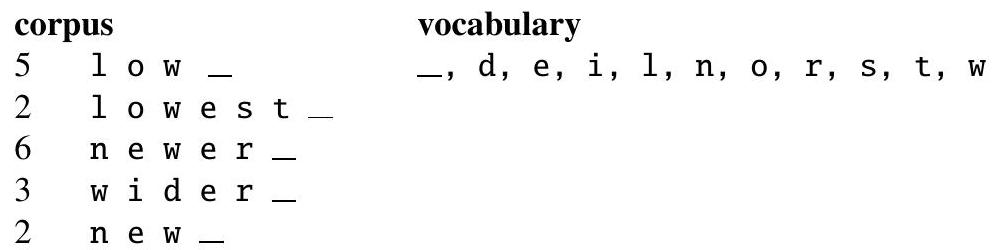
\includegraphics[max width=\textwidth, center]{2025_03_24_4f41283092a9d1f7a40eg-029}

The BPE algorithm first counts all pairs of adjacent symbols: the most frequent is the pair e r because it occurs in newer (frequency of 6) and wider (frequency of 3) for a total of 9 occurrences. ${ }^{2}$ We then merge these symbols, treating er as one symbol, and count again:

\footnotetext{2 Note that there can be ties; we could have instead chosen to merge $r$ \_ first, since that also has a frequency of 9 .
}\begin{verbatim}
corpus vocabulary
5 l o w _ _ , d, e, i, l, n, o, r, s, t, w, er
2 l o w e s t -
6 n e w er _
3 w i d er _
n n e w -
\end{verbatim}

Now the most frequent pair is er \textit{, which we merge; our system has learned that there should be a token for word-final er, represented as er}:

\begin{center}
\begin{tabular}{|c|c|}
\hline
corpus & vocabulary \\
\hline
5110 w - & $\ldots, d, e, i, l, n, o, r, s, t, w, e r, e r \_$ \\
\hline
2 l o w e s t - &  \\
\hline
6 n e w er\_ &  \\
\hline
3 w i d er\_ &  \\
\hline
2 n e w - &  \\
\hline
\end{tabular}
\end{center}

Next n e (total count of 8) get merged to ne:

\begin{center}
\begin{tabular}{|c|c|}
\hline
corpus & vocabulary \\
\hline
$51 \mathrm{ol} \mathrm{w}^{\text {- }}$ & 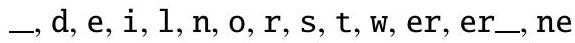
\includegraphics[max width=\textwidth]{2025_03_24_4f41283092a9d1f7a40eg-030(1)}
 \\
\hline
2 l o w e s t - &  \\
\hline
6 ne w er\_ &  \\
\hline
3 w i d er\_ &  \\
\hline
2 ne w \_ &  \\
\hline
\end{tabular}
\end{center}

If we continue, the next merges are:\\
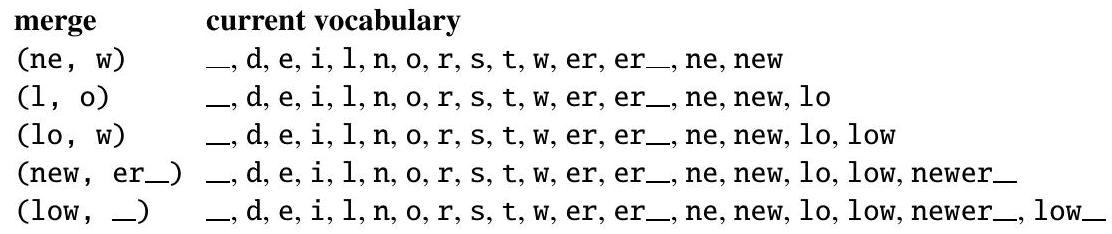
\includegraphics[max width=\textwidth, center]{2025_03_24_4f41283092a9d1f7a40eg-030}

$$
\begin{aligned}
& \text { function BYTE-PAIR ENCODING(strings } C \text {, number of merges } k \text { ) returns vocab } V \\
& \begin{array}{l}
V \leftarrow \text { all unique characters in } C \quad \text { \# initial set of tokens is characters } \\
\text { for } i=1 \text { to } k \text { do } \\
t_{L}, t_{R} \leftarrow \text { Most frequent pair of adjacent tokens in } C \\
t_{\text {NEW }} \leftarrow t_{L}+t_{R} \\
V \leftarrow V+t_{N E W} \\
\text { \# make new token by concatenating } \\
\text { Replace each occurrence of } t_{L} \text {, } t_{R} \text { in } C \text { with } t_{N E W} \quad \text { \# and update the corpus } \\
\text { return } V
\end{array}
\end{aligned}
$$

Figure 2.13 The token learner part of the BPE algorithm for taking a corpus broken up into individual characters or bytes, and learning a vocabulary by iteratively merging tokens. Figure adapted from Bostrom and Durrett (2020).

Once we've learned our vocabulary, the token segmenter is used to tokenize a test sentence. The token segmenter just runs on the merges we have learned from the training data on the test data. It runs them greedily, in the order we learned them. (Thus the frequencies in the test data don't play a role, just the frequencies in the training data). So first we segment each test sentence word into characters. Then we apply the first rule: replace every instance of er in the test corpus with er, and\\
then the second rule: replace every instance of er \_ in the test corpus with er\_, and so on. By the end, if the test corpus contained the character sequence $n$ e we r \textit{, it would be tokenized as a full word. But the characters of a new (unknown) word like lower \_ would be merged into the two tokens low er}.

Of course in real settings BPE is run with many thousands of merges on a very large input corpus. The result is that most words will be represented as full symbols, and only the very rare words (and unknown words) will have to be represented by their parts.

\subsection*{2.6 Word Normalization, Lemmatization and Stemming}
Word normalization is the task of putting words or tokens in a standard format. The simplest case of word normalization is case folding. Mapping everything to lower case means that Woodchuck and woodchuck are represented identically, which is very helpful for generalization in many tasks, such as information retrieval or speech recognition. For sentiment analysis and other text classification tasks, information extraction, and machine translation, by contrast, case can be quite helpful and case folding is generally not done. This is because maintaining the difference between, for example, US the country and us the pronoun can outweigh the advantage in generalization that case folding would have provided for other words. Sometimes we produce both cased (i.e. including both upper and lower case words or tokens) and uncased versions of language models.

Systems that use BPE or other kinds of bottom-up tokenization may do no further word normalization. In other NLP systems, we may want to do further normalizations, like choosing a single normal form for words with multiple forms like USA and US or uh-huh and uhhuh. This standardization may be valuable, despite the spelling information that is lost in the normalization process. For information retrieval or information extraction about the US, we might want to see information from documents whether they mention the US or the USA.

\subsection*{2.6.1 Lemmatization}
For other natural language processing situations we also want two morphologically different forms of a word to behave similarly. For example in web search, someone may type the string woodchucks but a useful system might want to also return pages that mention woodchuck with no $s$. This is especially common in morphologically complex languages like Polish, where for example the word Warsaw has different endings when it is the subject (Warszawa), or after a preposition like "in Warsaw" ( $w$ Warszawie), or "to Warsaw" (do Warszawy), and so on. Lemmatization is the task of determining that two words have the same root, despite their surface differences. The words am, are, and is have the shared lemma be; the words dinner and dinners both have the lemma dinner. Lemmatizing each of these forms to the same lemma will let us find all mentions of words in Polish like Warsaw. The lemmatized form of a sentence like He is reading detective stories would thus be He be read detective story.

How is lemmatization done? The most sophisticated methods for lemmatization involve complete morphological parsing of the word. Morphology is the study of the way words are built up from smaller meaning-bearing units called morphemes.\\
affix pheme of the word, supplying the main meaning-and affixes-adding "additional" meanings of various kinds. So, for example, the word fox consists of one morpheme (the morpheme fox) and the word cats consists of two: the morpheme cat and the morpheme $-s$. A morphological parser takes a word like cats and parses it into the two morphemes cat and $s$, or parses a Spanish word like amaren ('if in the future they would love') into the morpheme amar 'to love', and the morphological features 3PL (third person plural) and future subjunctive.

\section*{Stemming: The Porter Stemmer}
Lemmatization algorithms can be complex. For this reason we sometimes make use of a simpler but cruder method, which mainly consists of chopping off word-\\
stemming final affixes. This naive version of morphological analysis is called stemming. For example, the classic Porter stemmer (Porter, 1980), when applied to the following paragraph:

\begin{verbatim}
This was not the map we found in Billy Bones's chest, but
an accurate copy, complete in all things-names and heights
and soundings-with the single exception of the red crosses
and the written notes.
\end{verbatim}

produces the following stemmed output:\\
Thi wa not the map we found in Billi Bone s chest but an accur copi complet in all thing name and height and sound with the singl except of the red cross and the written note\\
The algorithm is based on rewrite rules run in series, with the output of each pass fed as input to the next pass. Some sample rules (more at \href{https://tartarus.org/}{https://tartarus.org/} martin/PorterStemmer/):

$$
\begin{aligned}
\text { ATIONAL } & \rightarrow \text { ATE (e.g., relational } \rightarrow \text { relate) } \\
\text { ING } & \rightarrow \epsilon \quad \text { if the stem contains a vowel (e.g., motoring } \rightarrow \text { motor) } \\
\text { SSES } & \rightarrow \text { SS } \quad(\text { e.g., grasses } \rightarrow \text { grass })
\end{aligned}
$$

Simple stemmers can be useful in cases where we need to collapse across different variants of the same lemma. Nonetheless, they are less commonly used in modern systems since they commit errors of both over-generalizing (lemmatizing policy to police) and under-generalizing (not lemmatizing European to Europe) (Krovetz, 1993).

\subsection*{2.7 Sentence Segmentation}
sentence segmentation

Sentence segmentation is another important step in text processing. The most useful cues for segmenting a text into sentences are punctuation, like periods, question marks, and exclamation points. Question marks and exclamation points are relatively unambiguous markers of sentence boundaries. Periods, on the other hand, are more ambiguous. The period character "." is ambiguous between a sentence boundary marker and a marker of abbreviations like $M r$. or Inc. The previous sentence that you just read showed an even more complex case of this ambiguity, in which the final period of Inc. marked both an abbreviation and the sentence boundary marker. For this reason, sentence tokenization and word tokenization may be addressed jointly.

In general, sentence tokenization methods work by first deciding (based on rules or machine learning) whether a period is part of the word or is a sentence-boundary marker. An abbreviation dictionary can help determine whether the period is part of a commonly used abbreviation; the dictionaries can be hand-built or machinelearned (Kiss and Strunk, 2006), as can the final sentence splitter. In the Stanford CoreNLP toolkit (Manning et al., 2014), for example sentence splitting is rule-based, a deterministic consequence of tokenization; a sentence ends when a sentence-ending punctuation (., !, or ?) is not already grouped with other characters into a token (such as for an abbreviation or number), optionally followed by additional final quotes or brackets.

\subsection*{2.8 Minimum Edit Distance}
Much of natural language processing is concerned with measuring how similar two strings are. For example in spelling correction, the user typed some erroneous string-let's say graffe-and we want to know what the user meant. The user probably intended a word that is similar to graffe. Among candidate similar words, the word giraffe, which differs by only one letter from graffe, seems intuitively to be more similar than, say grail or graf, which differ in more letters. Another example comes from coreference, the task of deciding whether two strings such as the following refer to the same entity:

\begin{verbatim}
Stanford Arizona Cactus Garden
Stanford University Arizona Cactus Garden
\end{verbatim}

Again, the fact that these two strings are very similar (differing by only one word) seems like useful evidence for deciding that they might be coreferent. Finally, string similarity is commonly used to measure the quality of the transcription produced by a speech recognition system, by asking how similar (in words) the transcript is to a reference transcript. A system whose transcript is off by many words is measurably worse than one which is only off by a few words.

Edit distance gives us a way to quantify these intuitions about string similarity.\\
minimum edit distance More formally, the minimum edit distance between two strings is defined as the minimum number of editing operations (operations like insertion, deletion, substitution) needed to transform one string into another.

The gap between intention and execution, for example, is 5 (delete an i , substitute e for n , substitute x for t , insert c , substitute u for n ). It's much easier to see this by looking at the most important visualization for string distances, an alignment between the two strings, shown in Fig. 2.14. Given two sequences, an alignment is a correspondence between substrings of the two sequences. Thus, we say I aligns with the empty string, N with E , and so on. Beneath the aligned strings is another representation; a series of symbols expressing an operation list for converting the top string into the bottom string: $\mathbf{d}$ for deletion, $\mathbf{s}$ for substitution, $\mathbf{i}$ for insertion.

We can also assign a particular cost or weight to each of these operations. The Levenshtein distance between two sequences is the simplest weighting factor in which each of the three operations has a cost of 1 (Levenshtein, 1966)-we assume that the substitution of a letter for itself, for example, $t$ for $t$, has zero cost. The Levenshtein distance between intention and execution is 5 . Levenshtein also proposed an alternative version of his metric in which each insertion or deletion has a cost of 1 and substitutions are not allowed. (This is equivalent to allowing substitution, but\\
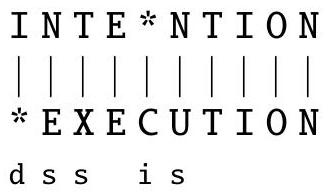
\includegraphics[max width=\textwidth, center]{2025_03_24_4f41283092a9d1f7a40eg-034}

Figure 2.14 Representing the minimum edit distance between two strings as an alignment. The final row gives the operation list for converting the top string into the bottom string: d for deletion, s for substitution, i for insertion.\\
giving each substitution a cost of 2 since any substitution can be represented by one insertion and one deletion). Using this version, the Levenshtein distance between intention and execution is 8 .

\subsection*{2.8.1 The Minimum Edit Distance Algorithm}
How do we find the minimum edit distance? We can think of this as a search task, in which we are searching for the shortest path-a sequence of edits-from one string to another.\\
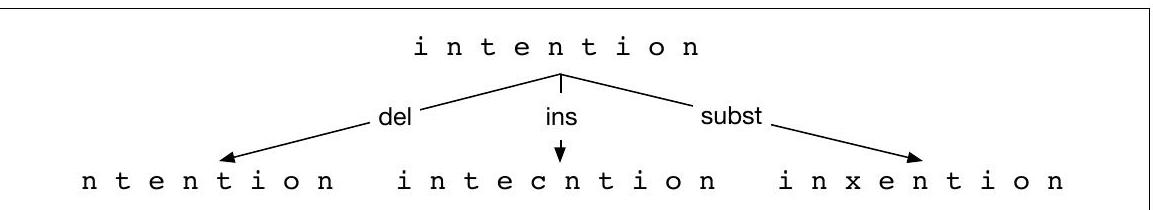
\includegraphics[max width=\textwidth, center]{2025_03_24_4f41283092a9d1f7a40eg-034(1)}

Figure 2.15 Finding the edit distance viewed as a search problem

The space of all possible edits is enormous, so we can't search naively. However, lots of distinct edit paths will end up in the same state (string), so rather than recomputing all those paths, we could just remember the shortest path to a state each time we saw it. We can do this by using dynamic programming. Dynamic programming is the name for a class of algorithms, first introduced by Bellman (1957), that apply a table-driven method to solve problems by combining solutions to subproblems. Some of the most commonly used algorithms in natural language processing make use of dynamic programming, such as the Viterbi algorithm (Chapter 17) and the CKY algorithm for parsing (Chapter 18).

The intuition of a dynamic programming problem is that a large problem can be solved by properly combining the solutions to various subproblems. Consider the shortest path of transformed words that represents the minimum edit distance between the strings intention and execution shown in Fig. 2.16.

Imagine some string (perhaps it is exention) that is in this optimal path (whatever it is). The intuition of dynamic programming is that if exention is in the optimal operation list, then the optimal sequence must also include the optimal path from intention to exention. Why? If there were a shorter path from intention to exention, then we could use it instead, resulting in a shorter overall path, and the optimal sequence wouldn't be optimal, thus leading to a contradiction.

The minimum edit distance algorithm was named by Wagner and Fischer (1974) but independently discovered by many people (see the Historical Notes section of Chapter 17).

Let's first define the minimum edit distance between two strings. Given two strings, the source string $X$ of length $n$, and target string $Y$ of length $m$, we'll define

\begin{verbatim}
i n t e n t i o n
n t e n t i o n
e t e n t i o n
e x e n t i o n
e x e n u t i o n
ex e cutt i o n
\end{verbatim}

Figure 2.16 Path from intention to execution.\\
$D[i, j]$ as the edit distance between $X[1 . . i]$ and $Y[1 . . j]$, i.e., the first $i$ characters of $X$ and the first $j$ characters of $Y$. The edit distance between $X$ and $Y$ is thus $D[n, m]$.

We'll use dynamic programming to compute $D[n, m]$ bottom up, combining solutions to subproblems. In the base case, with a source substring of length $i$ but an empty target string, going from $i$ characters to 0 requires $i$ deletes. With a target substring of length $j$ but an empty source going from 0 characters to $j$ characters requires $j$ inserts. Having computed $D[i, j]$ for small $i, j$ we then compute larger $D[i, j]$ based on previously computed smaller values. The value of $D[i, j]$ is computed by taking the minimum of the three possible paths through the matrix which arrive there:

\[
D[i, j]=\min \left\{\begin{array}{l}
D[i-1, j]+\operatorname{del}-\operatorname{cost}(\text { source }[i])  \tag{2.23}\\
D[i, j-1]+\operatorname{ins}-\operatorname{cost}(\text { target }[j]) \\
D[i-1, j-1]+\operatorname{sub}-\operatorname{cost}(\text { source }[i], \text { target }[j])
\end{array}\right.
\]

We mentioned above two versions of Levenshtein distance, one in which substitutions cost 1 and one in which substitutions cost 2 (i.e., are equivalent to an insertion plus a deletion). Let's here use that second version of Levenshtein distance in which the insertions and deletions each have a cost of 1 (ins-cost $(\cdot)=\operatorname{del}-\operatorname{cost}(\cdot)=1$ ), and substitutions have a cost of 2 (except substitution of identical letters has zero cost). Under this version of Levenshtein, the computation for $D[i, j]$ becomes:

\[
D[i, j]=\min \left\{\begin{array}{l}
D[i-1, j]+1  \tag{2.24}\\
D[i, j-1]+1 \\
D[i-1, j-1]+ \begin{cases}2 ; & \text { if } \operatorname{source}[i] \neq \operatorname{target}[j] \\
0 ; & \text { if } \operatorname{source}[i]=\operatorname{target}[j]\end{cases}
\end{array}\right.
\]

The algorithm is summarized in Fig. 2.17; Fig. 2.18 shows the results of applying the algorithm to the distance between intention and execution with the version of Levenshtein in Eq. 2.24.

Alignment Knowing the minimum edit distance is useful for algorithms like finding potential spelling error corrections. But the edit distance algorithm is important in another way; with a small change, it can also provide the minimum cost alignment between two strings. Aligning two strings is useful throughout speech and language processing. In speech recognition, minimum edit distance alignment is used to compute the word error rate (Chapter 16). Alignment plays a role in machine translation, in which sentences in a parallel corpus (a corpus with a text in two languages) need to be matched to each other.

To extend the edit distance algorithm to produce an alignment, we can start by visualizing an alignment as a path through the edit distance matrix. Figure 2.19

\begin{verbatim}
function Min-Edit-Distance(source, target) returns min-distance
\end{verbatim}

\begin{verbatim}
$n \leftarrow \operatorname{LENGTH}$ (source)
$m \leftarrow$ LENGTH(target)
Create a distance matrix $D[n+1, m+1]$
    \# Initialization: the zeroth row and column is the distance from the empty string
    $D[0,0]=0$
    for each row $i$ from 1 to $n$ do
        $D[i, 0] \leftarrow D[i-1,0]+\operatorname{del}-\operatorname{cost}($ source $[i])$
    for each column $j$ from 1 to $m$ do
        $D[0, j] \leftarrow D[0, j-1]+$ ins-cost $($ target $[j])$
    \# Recurrence relation:
    for each row $i$ from 1 to $n$ do
        for each column $j$ from 1 to $m$ do
            $D[i, j] \leftarrow \operatorname{Min}(D[i-1, j]+\operatorname{del-cost}($ source $[i])$,
                $D[i-1, j-1]+\operatorname{sub}-\operatorname{cost}($ source $[i]$, target $[j]$ ),
                $D[i, j-1]+\operatorname{ins}-\operatorname{cost}((\operatorname{target}[j]))$
    \# Termination
    return $D[\mathrm{n}, \mathrm{m}]$
\end{verbatim}

Figure 2.17 The minimum edit distance algorithm, an example of the class of dynamic programming algorithms. The various costs can either be fixed (e.g., $\forall x, \operatorname{ins}-\operatorname{cost}(x)=1$ ) or can be specific to the letter (to model the fact that some letters are more likely to be inserted than others). We assume that there is no cost for substituting a letter for itself (i.e., $\operatorname{sub}-\operatorname{cost}(x, x)=0)$.

\begin{center}
\begin{tabular}{|r|r|r|r|r|r|r|r|r|r|r|}
\hline
Src $\backslash$ Tar & $\#$ & $\mathbf{e}$ & $\mathbf{x}$ & $\mathbf{e}$ & $\mathbf{c}$ & $\mathbf{u}$ & $\mathbf{t}$ & $\mathbf{i}$ & $\mathbf{o}$ & $\mathbf{n}$ \\
\hline
$\#$ & 0 & 1 & 2 & 3 & 4 & 5 & 6 & 7 & 8 & 9 \\
\hline
$\mathbf{i}$ & 1 & 2 & 3 & 4 & 5 & 6 & 7 & 6 & 7 & 8 \\
\hline
$\mathbf{n}$ & 2 & 3 & 4 & 5 & 6 & 7 & 8 & 7 & 8 & 7 \\
\hline
$\mathbf{t}$ & 3 & 4 & 5 & 6 & 7 & 8 & 7 & 8 & 9 & 8 \\
\hline
$\mathbf{e}$ & 4 & 3 & 4 & 5 & 6 & 7 & 8 & 9 & 10 & 9 \\
\hline
$\mathbf{n}$ & 5 & 4 & 5 & 6 & 7 & 8 & 9 & 10 & 11 & 10 \\
\hline
$\mathbf{t}$ & 6 & 5 & 6 & 7 & 8 & 9 & 8 & 9 & 10 & 11 \\
\hline
$\mathbf{i}$ & 7 & 6 & 7 & 8 & 9 & 10 & 9 & 8 & 9 & 10 \\
\hline
$\mathbf{0}$ & 8 & 7 & 8 & 9 & 10 & 11 & 10 & 9 & 8 & 9 \\
\hline
$\mathbf{n}$ & 9 & 8 & 9 & 10 & 11 & 12 & 11 & 10 & 9 & 8 \\
\hline
\end{tabular}
\end{center}

Figure 2.18 Computation of minimum edit distance between intention and execution with the algorithm of Fig. 2.17, using Levenshtein distance with cost of 1 for insertions or deletions, 2 for substitutions.\\
shows this path with boldfaced cells. Each boldfaced cell represents an alignment of a pair of letters in the two strings. If two boldfaced cells occur in the same row, there will be an insertion in going from the source to the target; two boldfaced cells in the same column indicate a deletion.

Figure 2.19 also shows the intuition of how to compute this alignment path. The computation proceeds in two steps. In the first step, we augment the minimum edit distance algorithm to store backpointers in each cell. The backpointer from a cell points to the previous cell (or cells) that we came from in entering the current cell. We've shown a schematic of these backpointers in Fig. 2.19. Some cells have mul-\\
tiple backpointers because the minimum extension could have come from multiple previous cells. In the second step, we perform a backtrace. In a backtrace, we start from the last cell (at the final row and column), and follow the pointers back through the dynamic programming matrix. Each complete path between the final cell and the initial cell is a minimum distance alignment. Exercise 2.7 asks you to modify the minimum edit distance algorithm to store the pointers and compute the backtrace to output an alignment.

\begin{center}
\begin{tabular}{|r|r|r|r|r|r|r|r|r|r|r|}
\hline
 & $\#$ & $\mathbf{e}$ & $\mathbf{x}$ & $\mathbf{e}$ & $\mathbf{c}$ & $\mathbf{u}$ & $\mathbf{t}$ & $\mathbf{i}$ & $\mathbf{0}$ & $\mathbf{n}$ \\
\hline
$\#$ & 0 & $\leftarrow 1$ & $\leftarrow 2$ & $\leftarrow 3$ & $\leftarrow 4$ & $\leftarrow 5$ & $\leftarrow 6$ & $\leftarrow 7$ & $\leftarrow 8$ & $\leftarrow 9$ \\
\hline
$\mathbf{i}$ & $\uparrow \mathbf{1}$ & $\nwarrow \leftarrow \uparrow 2$ & $\nwarrow \leftarrow \uparrow 3$ & $\nwarrow \leftarrow \uparrow 4$ & $\nwarrow \leftarrow \uparrow 5$ & $\nwarrow \leftarrow \uparrow 6$ & $\nwarrow \leftarrow \uparrow 7$ & $\nwarrow 6$ & $\leftarrow 7$ & $\leftarrow 8$ \\
\hline
$\mathbf{n}$ & $\uparrow 2$ & $\nwarrow \leftarrow \uparrow \mathbf{3}$ & $\nwarrow \leftarrow \uparrow 4$ & $\nwarrow \leftarrow \uparrow 5$ & $\nwarrow \leftarrow \uparrow 6$ & $\nwarrow \leftarrow \uparrow 7$ & $\nwarrow \leftarrow \uparrow 8$ & $\uparrow 7$ & $\nwarrow \leftarrow \uparrow 8$ & $\nwarrow 7$ \\
\hline
$\mathbf{t}$ & $\uparrow 3$ & $\nwarrow \leftarrow \uparrow 4$ & $\nwarrow \leftarrow \uparrow \mathbf{5}$ & $\nwarrow \leftarrow \uparrow 6$ & $\nwarrow \leftarrow \uparrow 7$ & $\nwarrow \leftarrow \uparrow 8$ & $\nwarrow 7$ & $\leftarrow \uparrow 8$ & $\nwarrow \leftarrow \uparrow 9$ & $\uparrow 8$ \\
\hline
$\mathbf{e}$ & $\uparrow 4$ & $\nwarrow 3$ & $\leftarrow 4$ & $\nwarrow \leftarrow \mathbf{5}$ & $\leftarrow \mathbf{6}$ & $\leftarrow 7$ & $\leftarrow \uparrow 8$ & $\nwarrow \leftarrow \uparrow 9$ & $\nwarrow \leftarrow \uparrow 10$ & $\uparrow 9$ \\
\hline
$\mathbf{n}$ & $\uparrow 5$ & $\uparrow 4$ & $\nwarrow \leftarrow \uparrow 5$ & $\nwarrow \leftarrow \uparrow 6$ & $\nwarrow \leftarrow \uparrow 7$ & $\nwarrow \leftarrow \uparrow \mathbf{8}$ & $\nwarrow \leftarrow \uparrow 9$ & $\nwarrow \leftarrow \uparrow 10$ & $\nwarrow \leftarrow \uparrow 11$ & $\nwarrow \uparrow 10$ \\
\hline
$\mathbf{t}$ & $\uparrow 6$ & $\uparrow 5$ & $\nwarrow \leftarrow \uparrow 6$ & $\nwarrow \leftarrow \uparrow 7$ & $\nwarrow \leftarrow \uparrow 8$ & $\nwarrow \leftarrow \uparrow 9$ & $\nwarrow \mathbf{8}$ & $\leftarrow 9$ & $\leftarrow 10$ & $\leftarrow \uparrow 11$ \\
\hline
$\mathbf{i}$ & $\uparrow 7$ & $\uparrow 6$ & $\nwarrow \leftarrow \uparrow 7$ & $\nwarrow \leftarrow \uparrow 8$ & $\nwarrow \leftarrow \uparrow 9$ & $\nwarrow \leftarrow \uparrow 10$ & $\uparrow 9$ & $\nwarrow \mathbf{8}$ & $\leftarrow 9$ & $\leftarrow 10$ \\
\hline
$\mathbf{o}$ & $\uparrow 8$ & $\uparrow 7$ & $\nwarrow \leftarrow \uparrow 8$ & $\nwarrow \leftarrow \uparrow 9$ & $\nwarrow \leftarrow \uparrow 10$ & $\nwarrow \leftarrow \uparrow 11$ & $\uparrow 10$ & $\uparrow 9$ & $\nwarrow \mathbf{8}$ & $\leftarrow 9$ \\
\hline
$\mathbf{n}$ & $\uparrow 9$ & $\uparrow 8$ & $\nwarrow \leftarrow \uparrow 9$ & $\nwarrow \leftarrow \uparrow 10$ & $\nwarrow \leftarrow \uparrow 11$ & $\nwarrow \leftarrow \uparrow 12$ & $\uparrow 11$ & $\uparrow 10$ & $\uparrow 9$ & $\nwarrow \mathbf{8}$ \\
\hline\hline
\end{tabular}
\end{center}

Figure 2.19 When entering a value in each cell, we mark which of the three neighboring cells we came from with up to three arrows. After the table is full we compute an alignment (minimum edit path) by using a backtrace, starting at the $\mathbf{8}$ in the lower-right corner and following the arrows back. The sequence of bold cells represents one possible minimum cost alignment between the two strings, again using Levenshtein distance with cost of 1 for insertions or deletions, 2 for substitutions. Diagram design after Gusfield (1997).

While we worked our example with simple Levenshtein distance, the algorithm in Fig. 2.17 allows arbitrary weights on the operations. For spelling correction, for example, substitutions are more likely to happen between letters that are next to each other on the keyboard. The Viterbi algorithm is a probabilistic extension of minimum edit distance. Instead of computing the "minimum edit distance" between two strings, Viterbi computes the "maximum probability alignment" of one string with another. We'll discuss this more in Chapter 17.

\subsection*{2.9 Summary}
This chapter introduced a fundamental tool in language processing, the regular expression, and showed how to perform basic text normalization tasks including word segmentation and normalization, sentence segmentation, and stemming. We also introduced the important minimum edit distance algorithm for comparing strings. Here's a summary of the main points we covered about these ideas:

\begin{itemize}
  \item The regular expression language is a powerful tool for pattern-matching.
  \item Basic operations in regular expressions include concatenation of symbols, disjunction of symbols $([], \mid)$, counters $\left(*,+\right.$, and $\{n, m\}$ ), anchors $\left({ }^{\wedge}, \$\right)$ and precedence operators $(()$,$) .$
  \item Word tokenization and normalization are generally done by cascades of simple regular expression substitutions or finite automata.
  \item The Porter algorithm is a simple and efficient way to do stemming, stripping off affixes. It does not have high accuracy but may be useful for some tasks.
  \item The minimum edit distance between two strings is the minimum number of operations it takes to edit one into the other. Minimum edit distance can be computed by dynamic programming, which also results in an alignment of the two strings.
\end{itemize}

\section*{Bibliographical and Historical Notes}
Kleene 1951; 1956 first defined regular expressions and the finite automaton, based on the McCulloch-Pitts neuron. Ken Thompson was one of the first to build regular expressions compilers into editors for text searching (Thompson, 1968). His editor $e d$ included a command " $\mathrm{g} /$ regular expression/p", or Global Regular Expression Print, which later became the Unix grep utility.

Text normalization algorithms have been applied since the beginning of the field. One of the earliest widely used stemmers was Lovins (1968). Stemming was also applied early to the digital humanities, by Packard (1973), who built an affix-stripping morphological parser for Ancient Greek. Currently a wide variety of code for tokenization and normalization is available, such as the Stanford Tokenizer (\href{https://nlp.stanford.edu/software/tokenizer.shtml}{https://nlp.stanford.edu/software/tokenizer.shtml}) or specialized tokenizers for Twitter (O'Connor et al., 2010), or for sentiment (http: \href{//sentiment.christopherpotts.net/tokenizing.html}{//sentiment.christopherpotts.net/tokenizing.html}). See Palmer (2012) for a survey of text preprocessing. NLTK is an essential tool that offers both useful Python libraries (\href{https://www.nltk.org}{https://www.nltk.org}) and textbook descriptions (Bird et al., 2009) of many algorithms including text normalization and corpus interfaces.

For more on Herdan's law and Heaps' Law, see Herdan (1960, p. 28), Heaps (1978), Egghe (2007) and Baayen (2001); For more on edit distance, see Gusfield (1997). Our example measuring the edit distance from 'intention' to 'execution' was adapted from Kruskal (1983). There are various publicly available packages to compute edit distance, including Unix diff and the NIST sclite program (NIST, 2005).

In his autobiography Bellman (1984) explains how he originally came up with the term dynamic programming:\\[0pt]
"...The 1950s were not good years for mathematical research. [the] Secretary of Defense ...had a pathological fear and hatred of the word, research... I decided therefore to use the word, "programming". I wanted to get across the idea that this was dynamic, this was multistage... I thought, let's ... take a word that has an absolutely precise meaning, namely dynamic... it's impossible to use the word, dynamic, in a pejorative sense. Try thinking of some combination that will possibly give it a pejorative meaning. It's impossible. Thus, I thought dynamic programming was a good name. It was something not even a Congressman could object to."

\section*{Exercises}
2.1 Write regular expressions for the following languages.

\begin{enumerate}
  \item the set of all alphabetic strings;
  \item the set of all lower case alphabetic strings ending in a $b$;
  \item the set of all strings from the alphabet $a, b$ such that each $a$ is immediately preceded by and immediately followed by a $b$;\\
2.2 Write regular expressions for the following languages. By "word", we mean an alphabetic string separated from other words by whitespace, any relevant punctuation, line breaks, and so forth.
  \item the set of all strings with two consecutive repeated words (e.g., "Humbert Humbert" and "the the" but not "the bug" or "the big bug");
  \item all strings that start at the beginning of the line with an integer and that end at the end of the line with a word;
  \item all strings that have both the word grotto and the word raven in them (but not, e.g., words like grottos that merely contain the word grotto);
  \item write a pattern that places the first word of an English sentence in a register. Deal with punctuation.\\
2.3 Implement an ELIZA-like program, using substitutions such as those described on page 12. You might want to choose a different domain than a Rogerian psychologist, although keep in mind that you would need a domain in which your program can legitimately engage in a lot of simple repetition.\\
2.4 Compute the edit distance (using insertion cost 1 , deletion cost 1 , substitution cost 1) of "leda" to "deal". Show your work (using the edit distance grid).\\
2.5 Figure out whether drive is closer to brief or to divers and what the edit distance is to each. You may use any version of distance that you like.\\
2.6 Now implement a minimum edit distance algorithm and use your hand-computed results to check your code.\\
2.7 Augment the minimum edit distance algorithm to output an alignment; you will need to store pointers and add a stage to compute the backtrace.
\end{enumerate}

Predicting is difficult-especially about the future, as the old quip goes. But how about predicting something that seems much easier, like the next word someone is going to say? What word, for example, is likely to follow

The water of Walden Pond is so beautifully ...\\
You might conclude that a likely word is blue, or green, or clear, but probably not refrigerator nor this. In this chapter we formalize this intuition by intro-



\section*{N-gram Language Models}
 that predicts upcoming words. More formally, a language model assigns a probability to each possible next word, or equivalently gives a probability distribution over possible next works. Language models can also assign a probability to an entire sentence. Thus an LM could tell us that the following sequence has a much higher probability of appearing in a text:all of a sudden I notice three guys standing on the sidewalk\\
than does this same set of words in a different order:\\
on guys all I of notice sidewalk three a sudden standing the\\
Why would we want to predict upcoming words, or know the probability of a sentence? One reason is for generation: choosing contextually better words. For example we can correct grammar or spelling errors like Their are two midterms, in which There was mistyped as Their, or Everything has improve, in which improve should have been improved. The phrase There are is more probable than Their are, and has improved than has improve, so a language model can help users select the more grammatical variant. Or for a speech system to recognize that you said I will be back soonish and not I will be bassoon dish, it helps to know that back soonish is a more probable sequence. Language models can also help in augmentative and alternative communication (Trnka et al. 2007,\\
Kane et al. 2017). People can use AAC systems if they are physically unable to speak or sign but can instead use eye gaze or other movements to select words from a menu. Word prediction can be used to suggest likely words for the menu.

Word prediction is also central to NLP for another reason: large language models are built just by training them to predict words!! As we'll see in chapters 7-9, large language models learn an enormous amount about language solely from being trained to predict upcoming words from neighboring words.

In this chapter we introduce the simplest kind of language model: the n-gram\\
language model. An $n$-gram is a sequence of $n$ words: a 2-gram (which we'll call bigram) is a two-word sequence of words like The water, or water of, and a 3gram (a trigram) is a three-word sequence of words like The water of, or water of Walden. But we also (in a bit of terminological ambiguity) use the word ' $n$ gram' to mean a probabilistic model that can estimate the probability of a word given the $\mathrm{n}-1$ previous words, and thereby also to assign probabilities to entire sequences.

In later chapters we will introduce the much more powerful neural large language models, based on the transformer architecture of Chapter 9. But because n-grams have a remarkably simple and clear formalization, we use them to introduce some major concepts of large language modeling, including training and test sets, perplexity, sampling, and interpolation.

\subsection*{3.1 N-Grams}
Let's begin with the task of computing $P(w \mid h)$, the probability of a word $w$ given some history $h$. Suppose the history $h$ is "The water of Walden Pond is so beautifully " and we want to know the probability that the next word is blue:


\begin{equation*}
P(\text { blue|The water of Walden Pond is so beautifully) } \tag{3.1}
\end{equation*}


One way to estimate this probability is directly from relative frequency counts: take a very large corpus, count the number of times we see The water of Walden Pond is so beautifully, and count the number of times this is followed by blue. This would be answering the question "Out of the times we saw the history $h$, how many times was it followed by the word $w$ ", as follows:


\begin{align*}
& P(\text { blue } \mid \text { The water of Walden Pond is so beautifully })= \\
& \frac{C(\text { The water of Walden Pond is so beautifully blue })}{C(\text { The water of Walden Pond is so beautifully })}
\end{align*}


If we had a large enough corpus, we could compute these two counts and estimate the probability from Eq. 3.2. But even the entire web isn't big enough to give us good estimates for counts of entire sentences. This is because language is creative; new sentences are invented all the time, and we can't expect to get accurate counts for such large objects as entire sentences. For this reason, we'll need more clever ways to estimate the probability of a word $w$ given a history $h$, or the probability of an entire word sequence $W$.

Let's start with some notation. First, throughout this chapter we'll continue to refer to words, although in practice we usually compute language models over tokens like the BPE tokens of page 20. To represent the probability of a particular random variable $X_{i}$ taking on the value "the", or $P\left(X_{i}=\right.$ "the"), we will use the simplification $P($ the $)$. We'll represent a sequence of $n$ words either as $w_{1} \ldots w_{n}$ or $w_{1: n}$. Thus the expression $w_{1: n-1}$ means the string $w_{1}, w_{2}, \ldots, w_{n-1}$, but we'll also be using the equivalent notation $w_{<n}$, which can be read as "all the elements of $w$ from $w_{1}$ up to and including $w_{n-1}$ ". For the joint probability of each word in a sequence having a particular value $P\left(X_{1}=w_{1}, X_{2}=w_{2}, X_{3}=w_{3}, \ldots, X_{n}=w_{n}\right)$ we'll use $P\left(w_{1}, w_{2}, \ldots, w_{n}\right)$.

Now, how can we compute probabilities of entire sequences like $P\left(w_{1}, w_{2}, \ldots, w_{n}\right)$ ? One thing we can do is decompose this probability using the chain rule of proba-\\
bility:


\begin{align*}
P\left(X_{1} \ldots X_{n}\right) & =P\left(X_{1}\right) P\left(X_{2} \mid X_{1}\right) P\left(X_{3} \mid X_{1: 2}\right) \ldots P\left(X_{n} \mid X_{1: n-1}\right) \\
& =\prod_{k=1}^{n} P\left(X_{k} \mid X_{1: k-1}\right) \tag{3.3}
\end{align*}


Applying the chain rule to words, we get


\begin{align*}
P\left(w_{1: n}\right) & =P\left(w_{1}\right) P\left(w_{2} \mid w_{1}\right) P\left(w_{3} \mid w_{1: 2}\right) \ldots P\left(w_{n} \mid w_{1: n-1}\right) \\
& =\prod_{k=1}^{n} P\left(w_{k} \mid w_{1: k-1}\right) \tag{3.4}
\end{align*}


The chain rule shows the link between computing the joint probability of a sequence and computing the conditional probability of a word given previous words. Equation 3.4 suggests that we could estimate the joint probability of an entire sequence of words by multiplying together a number of conditional probabilities. But using the chain rule doesn't really seem to help us! We don't know any way to compute the exact probability of a word given a long sequence of preceding words, $P\left(w_{n} \mid w_{1: n-1}\right)$. As we said above, we can't just estimate by counting the number of times every word occurs following every long string in some corpus, because language is creative and any particular context might have never occurred before!

\subsection*{3.1.1 The Markov assumption}
The intuition of the n -gram model is that instead of computing the probability of a word given its entire history, we can approximate the history by just the last few words.

The bigram model, for example, approximates the probability of a word given all the previous words $P\left(w_{n} \mid w_{1: n-1}\right)$ by using only the conditional probability given the preceding word $P\left(w_{n} \mid w_{n-1}\right)$. In other words, instead of computing the probability


\begin{equation*}
P(\text { blue|The water of Walden Pond is so beautifully) } \tag{3.5}
\end{equation*}


we approximate it with the probability


\begin{equation*}
P(\text { blue|beautifully) } \tag{3.6}
\end{equation*}


When we use a bigram model to predict the conditional probability of the next word, we are thus making the following approximation:


\begin{equation*}
P\left(w_{n} \mid w_{1: n-1}\right) \approx P\left(w_{n} \mid w_{n-1}\right) \tag{3.7}
\end{equation*}


The assumption that the probability of a word depends only on the previous word is called a Markov assumption. Markov models are the class of probabilistic models that assume we can predict the probability of some future unit without looking too far into the past. We can generalize the bigram (which looks one word into the past) to the trigram (which looks two words into the past) and thus to the n-gram (which looks $n-1$ words into the past).

Let's see a general equation for this n -gram approximation to the conditional probability of the next word in a sequence. We'll use $N$ here to mean the n-gram\\
size, so $N=2$ means bigrams and $N=3$ means trigrams. Then we approximate the probability of a word given its entire context as follows:


\begin{equation*}
P\left(w_{n} \mid w_{1: n-1}\right) \approx P\left(w_{n} \mid w_{n-N+1: n-1}\right) \tag{3.8}
\end{equation*}


Given the bigram assumption for the probability of an individual word, we can compute the probability of a complete word sequence by substituting Eq. 3.7 into Eq. 3.4:


\begin{equation*}
P\left(w_{1: n}\right) \approx \prod_{k=1}^{n} P\left(w_{k} \mid w_{k-1}\right) \tag{3.9}
\end{equation*}


\subsection*{3.1.2 How to estimate probabilities}
maximum likelihood likelimation\\
normalize

How do we estimate these bigram or n-gram probabilities? An intuitive way to estimate probabilities is called maximum likelihood estimation or MLE. We get the MLE estimate for the parameters of an n-gram model by getting counts from a corpus, and normalizing the counts so that they lie between 0 and 1 . For probabilistic models, normalizing means dividing by some total count so that the resulting probabilities fall between 0 and 1 and sum to 1 .

For example, to compute a particular bigram probability of a word $w_{n}$ given a previous word $w_{n-1}$, we'll compute the count of the bigram $C\left(w_{n-1} w_{n}\right)$ and normalize by the sum of all the bigrams that share the same first word $w_{n-1}$ :


\begin{equation*}
P\left(w_{n} \mid w_{n-1}\right)=\frac{C\left(w_{n-1} w_{n}\right)}{\sum_{w} C\left(w_{n-1} w\right)} \tag{3.10}
\end{equation*}


We can simplify this equation, since the sum of all bigram counts that start with a given word $w_{n-1}$ must be equal to the unigram count for that word $w_{n-1}$ (the reader should take a moment to be convinced of this):


\begin{equation*}
P\left(w_{n} \mid w_{n-1}\right)=\frac{C\left(w_{n-1} w_{n}\right)}{C\left(w_{n-1}\right)} \tag{3.11}
\end{equation*}


Let's work through an example using a mini-corpus of three sentences. We'll first need to augment each sentence with a special symbol $<\mathrm{s}>$ at the beginning of the sentence, to give us the bigram context of the first word. We'll also need a special end-symbol </s>. ${ }^{1}$

\begin{verbatim}
<s> I am Sam </s>
<s> Sam I am </s>
<s> I do not like green eggs and ham </s>
\end{verbatim}

Here are the calculations for some of the bigram probabilities from this corpus

$$
\begin{array}{lll}
P(\mathrm{I}|<\mathrm{s}\rangle)=\frac{2}{3}=0.67 & P(\mathrm{Sam} \mid\langle\mathrm{s}\rangle)=\frac{1}{3}=0.33 & P(\mathrm{am} \mid \mathrm{I})=\frac{2}{3}=0.67 \\
P(</ \mathrm{s}>\mid \mathrm{Sam})=\frac{1}{2}=0.5 & P(\mathrm{Sam} \mid \mathrm{am})=\frac{1}{2}=0.5 & P(\mathrm{do} \mid \mathrm{I})=\frac{1}{3}=0.33
\end{array}
$$

For the general case of MLE n-gram parameter estimation:


\begin{equation*}
P\left(w_{n} \mid w_{n-N+1: n-1}\right)=\frac{C\left(w_{n-N+1: n-1} w_{n}\right)}{C\left(w_{n-N+1: n-1}\right)} \tag{3.12}
\end{equation*}


\footnotetext{1 We need the end-symbol to make the bigram grammar a true probability distribution. Without an endsymbol, instead of the sentence probabilities of all sentences summing to one, the sentence probabilities for all sentences of a given length would sum to one. This model would define an infinite set of probability distributions, with one distribution per sentence length. See Exercise 3.5.
}Equation 3.12 (like Eq. 3.11) estimates the n-gram probability by dividing the observed frequency of a particular sequence by the observed frequency of a prefix. This ratio is called a relative frequency. We said above that this use of relative frequencies as a way to estimate probabilities is an example of maximum likelihood estimation or MLE. In MLE, the resulting parameter set maximizes the likelihood of the training set $T$ given the model $M$ (i.e., $P(T \mid M)$ ). For example, suppose the word Chinese occurs 400 times in a corpus of a million words. What is the probability that a random word selected from some other text of, say, a million words will be the word Chinese? The MLE of its probability is $\frac{400}{1000000}$ or 0.0004 . Now 0.0004 is not the best possible estimate of the probability of Chinese occurring in all situations; it might turn out that in some other corpus or context Chinese is a very unlikely word. But it is the probability that makes it most likely that Chinese will occur 400 times in a million-word corpus. We present ways to modify the MLE estimates slightly to get better probability estimates in Section 3.6.

Let's move on to some examples from a real but tiny corpus, drawn from the now-defunct Berkeley Restaurant Project, a dialogue system from the last century that answered questions about a database of restaurants in Berkeley, California (Jurafsky et al., 1994). Here are some sample user queries (text-normalized, by lower casing and with punctuation striped) (a sample of 9332 sentences is on the website):

\begin{verbatim}
can you tell me about any good cantonese restaurants close by
tell me about chez panisse
i'm looking for a good place to eat breakfast
when is caffe venezia open during the day
\end{verbatim}

Figure 3.1 shows the bigram counts from part of a bigram grammar from textnormalized Berkeley Restaurant Project sentences. Note that the majority of the values are zero. In fact, we have chosen the sample words to cohere with each other; a matrix selected from a random set of eight words would be even more sparse.

\begin{center}
\begin{tabular}{lllllllll}
\hline
 & i & want & to & eat & chinese & food & lunch & spend \\
\hline
i & 5 & 827 & 0 & 9 & 0 & 0 & 0 & 2 \\
want & 2 & 0 & 608 & 1 & 6 & 6 & 5 & 1 \\
to & 2 & 0 & 4 & 686 & 2 & 0 & 6 & 211 \\
eat & 0 & 0 & 2 & 0 & 16 & 2 & 42 & 0 \\
chinese & 1 & 0 & 0 & 0 & 0 & 82 & 1 & 0 \\
food & 15 & 0 & 15 & 0 & 1 & 4 & 0 & 0 \\
lunch & 2 & 0 & 0 & 0 & 0 & 1 & 0 & 0 \\
spend & 1 & 0 & 1 & 0 & 0 & 0 & 0 & 0 \\
\hline
\end{tabular}
\end{center}

Figure 3.1 Bigram counts for eight of the words (out of $V=1446$ ) in the Berkeley Restaurant Project corpus of 9332 sentences. Zero counts are in gray. Each cell shows the count of the column label word following the row label word. Thus the cell in row $\mathbf{i}$ and column want means that want followed i 827 times in the corpus.

Figure 3.2 shows the bigram probabilities after normalization (dividing each cell in Fig. 3.1 by the appropriate unigram for its row, taken from the following set of unigram counts):

\begin{center}
\begin{tabular}{llllllll}
\hline
i & want to & eat & chinese & food & lunch & spend &  \\
\hline
2533 & 927 & 2417 & 746 & 158 & 1093 & 341 & 278 \\
\hline
\end{tabular}
\end{center}

\begin{center}
\begin{tabular}{lllllllll}
\hline
 & i & want & to & eat & chinese & food & lunch & spend \\
\hline
i & 0.002 & 0.33 & 0 & 0.0036 & 0 & 0 & 0 & 0.00079 \\
want & 0.0022 & 0 & 0.66 & 0.0011 & 0.0065 & 0.0065 & 0.0054 & 0.0011 \\
to & 0.00083 & 0 & 0.0017 & 0.28 & 0.00083 & 0 & 0.0025 & 0.087 \\
eat & 0 & 0 & 0.0027 & 0 & 0.021 & 0.0027 & 0.056 & 0 \\
chinese & 0.0063 & 0 & 0 & 0 & 0 & 0.52 & 0.0063 & 0 \\
food & 0.014 & 0 & 0.014 & 0 & 0.00092 & 0.0037 & 0 & 0 \\
lunch & 0.0059 & 0 & 0 & 0 & 0 & 0.0029 & 0 & 0 \\
spend & 0.0036 & 0 & 0.0036 & 0 & 0 & 0 & 0 & 0 \\
\hline
\end{tabular}
\end{center}

Figure 3.2 Bigram probabilities for eight words in the Berkeley Restaurant Project corpus of 9332 sentences. Zero probabilities are in gray.

Here are a few other useful probabilities:

$$
\begin{array}{ll}
P(\mathrm{i}|<\mathrm{s}\rangle)=0.25 & P(\text { english } \mid \text { want })=0.0011 \\
P(\text { food } \mid \text { english })=0.5 & P(</ \mathrm{s}\rangle \mid \text { food })=0.68
\end{array}
$$

Now we can compute the probability of sentences like I want English food or I want Chinese food by simply multiplying the appropriate bigram probabilities together, as follows:

$$
\begin{aligned}
& P(\langle\mathrm{~s}\rangle \text { i want english food }</ \mathrm{s}\rangle) \\
& =P(\mathrm{i}|<\mathrm{s}\rangle) P(\text { want } \mid \mathrm{i}) P(\text { english } \mid \text { want }) \\
& \\
& \quad P(\text { food } \mid \text { english }) P(</ \mathrm{s}>\mid \text { food }) \\
& = \\
& =0.25 \times 0.33 \times 0.0011 \times 0.5 \times 0.68 \\
& =000031
\end{aligned}
$$

We leave it as Exercise 3.2 to compute the probability of $i$ want chinese food.\\
What kinds of linguistic phenomena are captured in these bigram statistics? Some of the bigram probabilities above encode some facts that we think of as strictly syntactic in nature, like the fact that what comes after eat is usually a noun or an adjective, or that what comes after to is usually a verb. Others might be a fact about the personal assistant task, like the high probability of sentences beginning with the words $I$. And some might even be cultural rather than linguistic, like the higher probability that people are looking for Chinese versus English food.

\subsection*{3.1.3 Dealing with scale in large $n$-gram models}
In practice, language models can be very large, leading to practical issues.\\
Log probabilities Language model probabilities are always stored and computed in $\log$ space as $\log$ probabilities. This is because probabilities are (by definition) less than or equal to 1 , and so the more probabilities we multiply together, the smaller the product becomes. Multiplying enough n-grams together would result in numerical underflow. Adding in log space is equivalent to multiplying in linear space, so we combine $\log$ probabilities by adding them. By adding log probabilities instead of multiplying probabilities, we get results that are not as small. We do all computation and storage in log space, and just convert back into probabilities if we need to report probabilities at the end by taking the exp of the logprob:


\begin{equation*}
p_{1} \times p_{2} \times p_{3} \times p_{4}=\exp \left(\log p_{1}+\log p_{2}+\log p_{3}+\log p_{4}\right) \tag{3.13}
\end{equation*}


In practice throughout this book, we'll use $\log$ to mean natural $\log (\ln )$ when the base is not specified.

Longer context Although for pedagogical purposes we have only described bi-\\
trigram gram models, when there is sufficient training data we use trigram models, which condition on the previous two words, or 4-gram or 5-gram models. For these larger n-grams, we'll need to assume extra contexts to the left and right of the sentence end. For example, to compute trigram probabilities at the very beginning of the sentence, we use two pseudo-words for the first trigram (i.e., $P(\mathrm{I}|<\mathrm{s}\rangle\langle\mathrm{s}\rangle)$.

Some large n-gram datasets have been created, like the million most frequent n-grams drawn from the Corpus of Contemporary American English (COCA), a curated 1 billion word corpus of American English (Davies, 2020), Google's Web 5-gram corpus from 1 trillion words of English web text (Franz and Brants, 2006), or the Google Books Ngrams corpora (800 billion tokens from Chinese, English, French, German, Hebrew, Italian, Russian, and Spanish) (Lin et al., 2012a)).

It's even possible to use extremely long-range n-gram context. The infini-gram ( $\infty$-gram) project (Liu et al., 2024) allows n-grams of any length. Their idea is to avoid the expensive (in space and time) pre-computation of huge $n$-gram count tables. Instead, $n$-gram probabilities with arbitrary $n$ are computed quickly at inference time by using an efficient representation called suffix arrays. This allows computing of $n$-grams of every length for enormous corpora of 5 trillion tokens.

Efficiency considerations are important when building large n-gram language models. It is standard to quantize the probabilities using only 4-8 bits (instead of 8 -byte floats), store the word strings on disk and represent them in memory only as a 64-bit hash, and represent n-grams in special data structures like 'reverse tries'. It is also common to prune $n$-gram language models, for example by only keeping n-grams with counts greater than some threshold or using entropy to prune lessimportant n-grams (Stolcke, 1998). Efficient language model toolkits like KenLM (Heafield 2011, Heafield et al. 2013) use sorted arrays and use merge sorts to efficiently build the probability tables in a minimal number of passes through a large corpus.

\subsection*{3.2 Evaluating Language Models: Training and Test Sets}
The best way to evaluate the performance of a language model is to embed it in an application and measure how much the application improves. Such end-to-end evaluation is called extrinsic evaluation. Extrinsic evaluation is the only way to know if a particular improvement in the language model (or any component) is really going to help the task at hand. Thus for evaluating n-gram language models that are a component of some task like speech recognition or machine translation, we can compare the performance of two candidate language models by running the speech recognizer or machine translator twice, once with each language model, and seeing which gives the more accurate transcription.

Unfortunately, running big NLP systems end-to-end is often very expensive. Instead, it's helpful to have a metric that can be used to quickly evaluate potential improvements in a language model. An intrinsic evaluation metric is one that measures the quality of a model independent of any application. In the next section we'll introduce perplexity, which is the standard intrinsic metric for measuring language model performance, both for simple n-gram language models and for the more sophisticated neural large language models of Chapter 9.

In order to evaluate any machine learning model, we need to have at least three distinct data sets: the training set, the development set, and the test set.

The training set is the data we use to learn the parameters of our model; for simple n-gram language models it's the corpus from which we get the counts that we normalize into the probabilities of the n-gram language model.

The test set is a different, held-out set of data, not overlapping with the training set, that we use to evaluate the model. We need a separate test set to give us an unbiased estimate of how well the model we trained can generalize when we apply it to some new unknown dataset. A machine learning model that perfectly captured the training data, but performed terribly on any other data, wouldn't be much use when it comes time to apply it to any new data or problem! We thus measure the quality of an n-gram model by its performance on this unseen test set or test corpus.

How should we choose a training and test set? The test set should reflect the language we want to use the model for. If we're going to use our language model for speech recognition of chemistry lectures, the test set should be text of chemistry lectures. If we're going to use it as part of a system for translating hotel booking requests from Chinese to English, the test set should be text of hotel booking requests. If we want our language model to be general purpose, then the test set should be drawn from a wide variety of texts. In such cases we might collect a lot of texts from different sources, and then divide it up into a training set and a test set. It's important to do the dividing carefully; if we're building a general purpose model, we don't want the test set to consist of only text from one document, or one author, since that wouldn't be a good measure of general performance.

Thus if we are given a corpus of text and want to compare the performance of two different n-gram models, we divide the data into training and test sets, and train the parameters of both models on the training set. We can then compare how well the two trained models fit the test set.

But what does it mean to "fit the test set"? The standard answer is simple: whichever language model assigns a higher probability to the test set-which means it more accurately predicts the test set-is a better model. Given two probabilistic models, the better model is the one that better predicts the details of the test data, and hence will assign a higher probability to the test data.

Since our evaluation metric is based on test set probability, it's important not to let the test sentences into the training set. Suppose we are trying to compute the probability of a particular "test" sentence. If our test sentence is part of the training corpus, we will mistakenly assign it an artificially high probability when it occurs in the test set. We call this situation training on the test set. Training on the test set introduces a bias that makes the probabilities all look too high, and causes huge inaccuracies in perplexity, the probability-based metric we introduce below.

Even if we don't train on the test set, if we test our language model on the test set many times after making different changes, we might implicitly tune to its characteristics, by noticing which changes seem to make the model better. For this reason, we only want to run our model on the test set once, or a very few number of times, once we are sure our model is ready.

For this reason we normally instead have a third dataset called a development test set or, devset. We do all our testing on this dataset until the very end, and then we test on the test set once to see how good our model is.

How do we divide our data into training, development, and test sets? We want our test set to be as large as possible, since a small test set may be accidentally unrepresentative, but we also want as much training data as possible. At the minimum, we would want to pick the smallest test set that gives us enough statistical power to measure a statistically significant difference between two potential models. It's\\
important that the devset be drawn from the same kind of text as the test set, since its goal is to measure how we would do on the test set.

\subsection*{3.3 Evaluating Language Models: Perplexity}
We said above that we evaluate language models based on which one assigns a higher probability to the test set. A better model is better at predicting upcoming words, and so it will be less surprised by (i.e., assign a higher probability to) each word when it occurs in the test set. Indeed, a perfect language model would correctly guess each next word in a corpus, assigning it a probability of 1 , and all the other words a probability of zero. So given a test corpus, a better language model will assign a higher probability to it than a worse language model.

But in fact, we do not use raw probability as our metric for evaluating language models. The reason is that the probability of a test set (or any sequence) depends on the number of words or tokens in it; the probability of a test set gets smaller the longer the text. We'd prefer a metric that is per-word, normalized by length, so we could compare across texts of different lengths. The metric we use is, a function of probability called perplexity, is one of the most important metrics in NLP, used for evaluating large language models as well as n-gram models.\\
perplexity The perplexity (sometimes abbreviated as PP or PPL) of a language model on a test set is the inverse probability of the test set (one over the probability of the test set), normalized by the number of words (or tokens). For this reason it's sometimes called the per-word or per-token perplexity. We normalize by the number of words $N$ by taking the $N$ th root. For a test set $W=w_{1} w_{2} \ldots w_{N}$,:


\begin{align*}
\operatorname{perplexity}(W) & =P\left(w_{1} w_{2} \ldots w_{N}\right)^{-\frac{1}{N}}  \tag{3.14}\\
& =\sqrt[N]{\frac{1}{P\left(w_{1} w_{2} \ldots w_{N}\right)}}
\end{align*}


Or we can use the chain rule to expand the probability of $W$ :


\begin{equation*}
\operatorname{perplexity}(W)=\sqrt[N]{\prod_{i=1}^{N} \frac{1}{P\left(w_{i} \mid w_{1} \ldots w_{i-1}\right)}} \tag{3.15}
\end{equation*}


Note that because of the inverse in Eq. 3.15, the higher the probability of the word sequence, the lower the perplexity. Thus the the lower the perplexity of a model on the data, the better the model. Minimizing perplexity is equivalent to maximizing the test set probability according to the language model. Why does perplexity use the inverse probability? It turns out the inverse arises from the original definition of perplexity from cross-entropy rate in information theory; for those interested, the explanation is in the advanced Section 3.7. Meanwhile, we just have to remember that perplexity has an inverse relationship with probability.

The details of computing the perplexity of a test set $W$ depends on which language model we use. Here's the perplexity of $W$ with a unigram language model (just the geometric mean of the inverse of the unigram probabilities):


\begin{equation*}
\operatorname{perplexity}(W)=\sqrt[N]{\prod_{i=1}^{N} \frac{1}{P\left(w_{i}\right)}} \tag{3.16}
\end{equation*}


The perplexity of $W$ computed with a bigram language model is still a geometric mean, but now of the inverse of the bigram probabilities:


\begin{equation*}
\operatorname{perplexity}(W)=\sqrt[N]{\prod_{i=1}^{N} \frac{1}{P\left(w_{i} \mid w_{i-1}\right)}} \tag{3.17}
\end{equation*}


What we generally use for word sequence in Eq. 3.15 or Eq. 3.17 is the entire sequence of words in some test set. Since this sequence will cross many sentence boundaries, if our vocabulary includes a between-sentence token $<$ EOS $>$ or separate begin- and end-sentence markers  and  then we can include them in the probability computation. If we do, then we also include one token per sentence in the total count of word tokens $N .{ }^{2}$

We mentioned above that perplexity is a function of both the text and the language model: given a text $W$, different language models will have different perplexities. Because of this, perplexity can be used to compare different language models. For example, here we trained unigram, bigram, and trigram grammars on 38 million words from the Wall Street Journal newspaper. We then computed the perplexity of each of these models on a WSJ test set using Eq. 3.16 for unigrams, Eq. 3.17 for bigrams, and the corresponding equation for trigrams. The table below shows the perplexity of the 1.5 million word test set according to each of the language models.

\begin{center}
\begin{tabular}{llll}
\hline
 & Unigram & Bigram & Trigram \\
\hline
Perplexity & 962 & 170 & 109 \\
\hline
\end{tabular}
\end{center}

As we see above, the more information the $n$-gram gives us about the word sequence, the higher the probability the $n$-gram will assign to the string. A trigram model is less surprised than a unigram model because it has a better idea of what words might come next, and so it assigns them a higher probability. And the higher the probability, the lower the perplexity (since as Eq. 3.15 showed, perplexity is related inversely to the probability of the test sequence according to the model). So a lower perplexity tells us that a language model is a better predictor of the test set.

Note that in computing perplexities, the language model must be constructed without any knowledge of the test set, or else the perplexity will be artificially low. And the perplexity of two language models is only comparable if they use identical vocabularies.

An (intrinsic) improvement in perplexity does not guarantee an (extrinsic) improvement in the performance of a language processing task like speech recognition or machine translation. Nonetheless, because perplexity usually correlates with task improvements, it is commonly used as a convenient evaluation metric. Still, when possible a model's improvement in perplexity should be confirmed by an end-to-end evaluation on a real task.

\subsection*{3.3.1 Perplexity as Weighted Average Branching Factor}
It turns out that perplexity can also be thought of as the weighted average branching factor of a language. The branching factor of a language is the number of possible next words that can follow any word. For example consider a mini artificial

\footnotetext{2 For example if we use both begin and end tokens, we would include the end-of-sentence marker </s $>$ but not the beginning-of-sentence marker <s> in our count of $N$; This is because the end-sentence token is followed directly by the begin-sentence token with probability almost 1 , so we don't want the probability of that fake transition to influence our perplexity.
}
language that is deterministic (no probabilities), any word can follow any word, and whose vocabulary consists of only three colors:\\
\$\$

\begin{equation*}
L=\{\text { red, blue, green }\} \tag{3.18}
\end{equation*}

\$\$

The branching factor of this language is 3 .\\
Now let's make a probabilistic version of the same LM, let's call it $A$, where each word follows each other with equal probability $\frac{1}{3}$ (it was trained on a training set with equal counts for the 3 colors), and a test set $T=$ "red red red red blue".

Let's first convince ourselves that if we compute the perplexity of this artificial digit language on this test set (or any such test set) we indeed get 3. By Eq. 3.15, the perplexity of $A$ on $T$ is:


\begin{align*}
\operatorname{perplexity}_{A}(T) & =P_{A}(\text { red red red red blue })^{-\frac{1}{5}} \\
& =\left(\left(\frac{1}{3}\right)^{5}\right)^{-\frac{1}{5}} \\
& =\left(\frac{1}{3}\right)^{-1}=3 \tag{3.19}
\end{align*}


But now suppose red was very likely in the training set a different LM $B$, and so $B$ has the following probabilities:


\begin{equation*}
P(\mathrm{red})=0.8 \quad P(\text { green })=0.1 \quad P(\text { blue })=0.1 \tag{3.20}
\end{equation*}


We should expect the perplexity of the same test set red red red red blue for language model $B$ to be lower since most of the time the next color will be red, which is very predictable, i.e. has a high probability. So the probability of the test set will be higher, and since perplexity is inversely related to probability, the perplexity will be lower. Thus, although the branching factor is still 3 , the perplexity or weighted branching factor is smaller:


\begin{align*}
\operatorname{perplexity~}_{B}(T) & =P_{B}(\text { red red red red blue })^{-1 / 5} \\
& =0.04096^{-\frac{1}{5}} \\
& =0.527^{-1}=1.89 \tag{3.21}
\end{align*}


\subsection*{3.4 Sampling sentences from a language model}
One important way to visualize what kind of knowledge a language model embodies is to sample from it. Sampling from a distribution means to choose random points according to their likelihood. Thus sampling from a language model-which represents a distribution over sentences-means to generate some sentences, choosing each sentence according to its likelihood as defined by the model. Thus we are more likely to generate sentences that the model thinks have a high probability and less likely to generate sentences that the model thinks have a low probability.

This technique of visualizing a language model by sampling was first suggested very early on by Shannon (1948) and Miller and Selfridge (1950). It's simplest to visualize how this works for the unigram case. Imagine all the words of the English language covering the number line between 0 and 1 , each word covering an interval\\
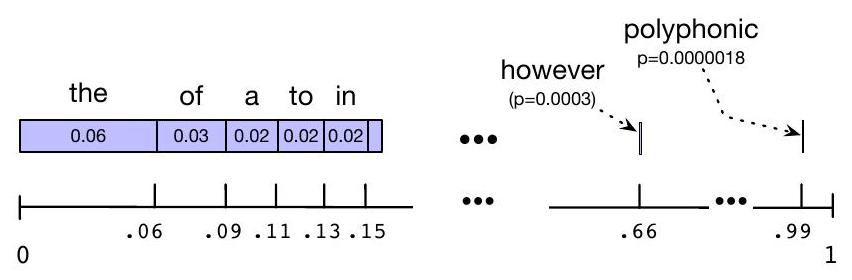
\includegraphics[max width=\textwidth, center]{2025_03_24_4f41283092a9d1f7a40eg-051}

Figure 3.3 A visualization of the sampling distribution for sampling sentences by repeatedly sampling unigrams. The blue bar represents the relative frequency of each word (we've ordered them from most frequent to least frequent, but the choice of order is arbitrary). The number line shows the cumulative probabilities. If we choose a random number between 0 and 1 , it will fall in an interval corresponding to some word. The expectation for the random number to fall in the larger intervals of one of the frequent words (the, of, $a$ ) is much higher than in the smaller interval of one of the rare words (polyphonic).\\
proportional to its frequency. Fig. 3.3 shows a visualization, using a unigram LM computed from the text of this book. We choose a random value between 0 and 1 , find that point on the probability line, and print the word whose interval includes this chosen value. We continue choosing random numbers and generating words until we randomly generate the sentence-final token </s>.

We can use the same technique to generate bigrams by first generating a random bigram that starts with $<\mathrm{s}\rangle$ (according to its bigram probability). Let's say the second word of that bigram is $w$. We next choose a random bigram starting with $w$ (again, drawn according to its bigram probability), and so on.

\subsection*{3.5 Generalizing vs. overfitting the training set}
The n-gram model, like many statistical models, is dependent on the training corpus. One implication of this is that the probabilities often encode specific facts about a given training corpus. Another implication is that n-grams do a better and better job of modeling the training corpus as we increase the value of $N$.

We can use the sampling method from the prior section to visualize both of these facts! To give an intuition for the increasing power of higher-order n-grams, Fig. 3.4 shows random sentences generated from unigram, bigram, trigram, and 4gram models trained on Shakespeare's works.

The longer the context, the more coherent the sentences. The unigram sentences show no coherent relation between words nor any sentence-final punctuation. The bigram sentences have some local word-to-word coherence (especially considering punctuation as words). The trigram sentences are beginning to look a lot like Shakespeare. Indeed, the 4-gram sentences look a little too much like Shakespeare. The words It cannot be but so are directly from King John. This is because, not to put the knock on Shakespeare, his oeuvre is not very large as corpora go ( $N=884,647, V=29,066$ ), and our n-gram probability matrices are ridiculously sparse. There are $V^{2}=844,000,000$ possible bigrams alone, and the number of possible 4 -grams is $V^{4}=7 \times 10^{17}$. Thus, once the generator has chosen the first 3-gram (It cannot be), there are only seven possible next words for the 4th element (but, I, that, thus, this, and the period).

To get an idea of the dependence on the training set, let's look at LMs trained on a completely different corpus: the Wall Street Journal (WSJ) newspaper. Shakespeare

\begin{verbatim}
                                    -To him swallowed confess hear both. Which. Of save on trail for are ay device and
1 rote life have
gram -Hill he late speaks; or! a more to leg less first you enter
-Why dost stand forth thy canopy, forsooth; he is this palpable hit the King Henry. Live
2 king. Follow.
gram -What means, sir. I confess she? then all sorts, he is trim, captain.
    -Fly, and will rid me these news of price. Therefore the sadness of parting, as they say,
$3 \quad$-Fly, and
gram -This shall forbid it should be branded, if renown made it empty.
    -King Henry. What! I will go seek the traitor Gloucester. Exeunt some of the watch. A
    great banquet serv'd in;
    gram -It cannot be but so.
\end{verbatim}

Figure 3.4 Eight sentences randomly generated from four n-grams computed from Shakespeare's works. All characters were mapped to lower-case and punctuation marks were treated as words. Output is hand-corrected for capitalization to improve readability.\\
and the WSJ are both English, so we might have expected some overlap between our n -grams for the two genres. Fig. 3.5 shows sentences generated by unigram, bigram, and trigram grammars trained on 40 million words from WSJ.

\begin{center}
\begin{tabular}{l}
\hline
1\begin{tabular}{l}
Months the my and issue of year foreign new exchange's september \\
were recession exchange new endorsed a acquire to six executives \\
\end{tabular} \\
gram \\
\begin{tabular}{l}
Last December through the way to preserve the Hudson corporation N. \\
gram \\
\end{tabular} \\
\begin{tabular}{l}
B. C. Taylor would seem to complete the major central planners one \\
point five percent of U. S. E. has already old M. X. corporation of living \\
on information such as more frequently fishing to keep her \\
They also point to ninety nine point six billion dollars from two hundred \\
four oh six three percent of the rates of interest stores as Mexico and \\
Brazil on market conditions \\
\end{tabular} \\
\hline
grare 3.5 \\
\hline
\end{tabular}
\end{center}

Compare these examples to the pseudo-Shakespeare in Fig. 3.4. While they both model "English-like sentences", there is no overlap in the generated sentences, and little overlap even in small phrases. Statistical models are pretty useless as predictors if the training sets and the test sets are as different as Shakespeare and the WSJ.

How should we deal with this problem when we build n-gram models? One step is to be sure to use a training corpus that has a similar genre to whatever task we are trying to accomplish. To build a language model for translating legal documents, we need a training corpus of legal documents. To build a language model for a question-answering system, we need a training corpus of questions.

It is equally important to get training data in the appropriate dialect or variety, especially when processing social media posts or spoken transcripts. For example some tweets will use features of African American English (AAE) - the name for the many variations of language used in African American communities (King, 2020). Such features can include words like finna-an auxiliary verb that marks immediate future tense -that don't occur in other varieties, or spellings like den for then, in tweets like this one (Blodgett and O'Connor, 2017):\\
(3.22) Bored af den my phone finna die!!!\\
while tweets from English-based languages like Nigerian Pidgin have markedly different vocabulary and n-gram patterns from American English (Jurgens et al., 2017):\\
(3.23) @username R u a wizard or wat gan sef: in d mornin - u tweet, afternoon - u tweet, nyt gan u dey tweet. beta get ur IT placement wiv twitter

Is it possible for the testset nonetheless to have a word we have never seen before? What happens if the word Jurafsky never occurs in our training set, but pops up in the test set? The answer is that although words might be unseen, we normally run our NLP algorithms not on words but on subword tokens. With subword tokenization (like the BPE algorithm of Chapter 2) any word can be modeled as a sequence of known smaller subwords, if necessary by a sequence of tokens corresponding to individual letters. So although for convenience we've been referring to words in this chapter, the language model vocabulary is normally the set of tokens rather than words, and in this way the test set can never contain unseen tokens.

\subsection*{3.6 Smoothing, Interpolation, and Backoff}
There is a problem with using maximum likelihood estimates for probabilities: any finite training corpus will be missing some perfectly acceptable English word sequences. That is, cases where a particular n-gram never occurs in the training data but appears in the test set. Perhaps our training corpus has the words ruby and slippers in it but just happens not to have the phrase ruby slippers.

These unseen sequences or zeros-sequences that don't occur in the training set but do occur in the test set-are a problem for two reasons. First, their presence means we are underestimating the probability of word sequences that might occur, which hurts the performance of any application we want to run on this data. Second, if the probability of any word in the test set is 0 , the probability of the whole test set is 0 . Perplexity is defined based on the inverse probability of the test set. Thus if some words in context have zero probability, we can't compute perplexity at all, since we can't divide by 0 !

The standard way to deal with putative "zero probability n-grams" that should really have some non-zero probability is called smoothing or discounting. Smoothing algorithms shave off a bit of probability mass from some more frequent events and give it to unseen events. Here we'll introduce some simple smoothing algorithms: Laplace (add-one) smoothing, stupid backoff, and $n$-gram interpolation.

\subsection*{3.6.1 Laplace Smoothing}
The simplest way to do smoothing is to add one to all the n-gram counts, before we normalize them into probabilities. All the counts that used to be zero will now have a count of 1 , the counts of 1 will be 2 , and so on. This algorithm is called in modern n-gram models, but it usefully introduces many of the concepts that we see in other smoothing algorithms, gives a useful baseline, and is also a practical smoothing algorithm for other tasks like text classification (Chapter 4).

Let's start with the application of Laplace smoothing to unigram probabilities. Recall that the unsmoothed maximum likelihood estimate of the unigram probability\\
of the word $w_{i}$ is its count $c_{i}$ normalized by the total number of word tokens $N$ :

$$
P\left(w_{i}\right)=\frac{c_{i}}{N}
$$

Laplace smoothing merely adds one to each count (hence its alternate name addone smoothing). Since there are $V$ words in the vocabulary and each one was incremented, we also need to adjust the denominator to take into account the extra $V$ observations. (What happens to our $P$ values if we don't increase the denominator?)


\begin{equation*}
P_{\text {Laplace }}\left(w_{i}\right)=\frac{c_{i}+1}{N+V} \tag{3.24}
\end{equation*}


Now that we have the intuition for the unigram case, let's smooth our Berkeley Restaurant Project bigrams. Figure 3.6 shows the add-one smoothed counts for the bigrams in Fig. 3.1.

\begin{center}
\begin{tabular}{lllllllll}
\hline
 & i & want & to & eat & chinese & food & lunch & spend \\
\hline
i & 6 & 828 & 1 & 10 & 1 & 1 & 1 & 3 \\
want & 3 & 1 & 609 & 2 & 7 & 7 & 6 & 2 \\
to & 3 & 1 & 5 & 687 & 3 & 1 & 7 & 212 \\
eat & 1 & 1 & 3 & 1 & 17 & 3 & 43 & 1 \\
chinese & 2 & 1 & 1 & 1 & 1 & 83 & 2 & 1 \\
food & 16 & 1 & 16 & 1 & 2 & 5 & 1 & 1 \\
lunch & 3 & 1 & 1 & 1 & 1 & 2 & 1 & 1 \\
spend & 2 & 1 & 2 & 1 & 1 & 1 & 1 & 1 \\
\hline
\end{tabular}
\end{center}

Figure 3.6 Add-one smoothed bigram counts for eight of the words (out of $V=1446$ ) in the Berkeley Restaurant Project corpus of 9332 sentences. Previously-zero counts are in gray.

Figure 3.7 shows the add-one smoothed probabilities for the bigrams in Fig. 3.2, computed by Eq. 3.26 below. Recall that normal bigram probabilities are computed by normalizing each row of counts by the unigram count:


\begin{equation*}
P_{\mathrm{MLE}}\left(w_{n} \mid w_{n-1}\right)=\frac{C\left(w_{n-1} w_{n}\right)}{C\left(w_{n-1}\right)} \tag{3.25}
\end{equation*}


For add-one smoothed bigram counts, we need to augment the unigram count in the denominator by the number of total word types in the vocabulary $V$. We can see why this is in the following equation, which makes it explicit that the unigram count in the denominator is really the sum over all the bigrams that start with $w_{n-1}$. Since we add one to each of these, and there are $V$ of them, we add a total of $V$ to the denominator:


\begin{equation*}
P_{\text {Laplace }}\left(w_{n} \mid w_{n-1}\right)=\frac{C\left(w_{n-1} w_{n}\right)+1}{\sum_{w}\left(C\left(w_{n-1} w\right)+1\right)}=\frac{C\left(w_{n-1} w_{n}\right)+1}{C\left(w_{n-1}\right)+V} \tag{3.26}
\end{equation*}


Thus, each of the unigram counts given on page 36 will need to be augmented by $V=$ 1446. The result, using Eq. 3.26, is the smoothed bigram probabilities in Fig. 3.7.

One useful visualization technique is to reconstruct an adjusted count matrix so we can see how much a smoothing algorithm has changed the original counts. This adjusted count $C^{*}$ is the count that, if divided by $C\left(w_{n-1}\right)$, would result in the smoothed probability. This adjusted count is easier to compare directly with the MLE counts. That is, the Laplace probability can equally be expressed as the adjusted count divided by the (non-smoothed) denominator from Eq. 3.25:

$$
P_{\text {Laplace }}\left(w_{n} \mid w_{n-1}\right)=\frac{C\left(w_{n-1} w_{n}\right)+1}{C\left(w_{n-1}\right)+V}=\frac{C^{*}\left(w_{n-1} w_{n}\right)}{C\left(w_{n-1}\right)}
$$

\begin{center}
\begin{tabular}{lllllllll}
\hline
 & i & want & to & eat & chinese & food & lunch & spend \\
\hline
i & 0.0015 & 0.21 & 0.00025 & 0.0025 & 0.00025 & 0.00025 & 0.00025 & 0.00075 \\
want & 0.0013 & 0.00042 & 0.26 & 0.00084 & 0.0029 & 0.0029 & 0.0025 & 0.00084 \\
to & 0.00078 & 0.00026 & 0.0013 & 0.18 & 0.00078 & 0.00026 & 0.0018 & 0.055 \\
eat & 0.00046 & 0.00046 & 0.0014 & 0.00046 & 0.0078 & 0.0014 & 0.02 & 0.00046 \\
chinese & 0.0012 & 0.00062 & 0.00062 & 0.00062 & 0.00062 & 0.052 & 0.0012 & 0.00062 \\
food & 0.0063 & 0.00039 & 0.0063 & 0.00039 & 0.00079 & 0.002 & 0.00039 & 0.00039 \\
lunch & 0.0017 & 0.00056 & 0.00056 & 0.00056 & 0.00056 & 0.0011 & 0.00056 & 0.00056 \\
spend & 0.0012 & 0.00058 & 0.0012 & 0.00058 & 0.00058 & 0.00058 & 0.00058 & 0.00058 \\
\hline
\end{tabular}
\end{center}

Figure 3.7 Add-one smoothed bigram probabilities for eight of the words (out of $V=1446$ ) in the BeRP corpus of 9332 sentences computed by Eq. 3.26. Previously-zero probabilities are in gray.

Rearranging terms, we can solve for $C^{*}\left(w_{n-1} w_{n}\right)$ :


\begin{equation*}
C^{*}\left(w_{n-1} w_{n}\right)=\frac{\left[C\left(w_{n-1} w_{n}\right)+1\right] \times C\left(w_{n-1}\right)}{C\left(w_{n-1}\right)+V} \tag{3.27}
\end{equation*}


Figure 3.8 shows the reconstructed counts, computed by Eq. 3.27.

\begin{center}
\begin{tabular}{lllllllll}
\hline
 & $\mathbf{i}$ & want & to & eat & chinese & food & lunch & spend \\
\hline
i & 3.8 & 527 & 0.64 & 6.4 & 0.64 & 0.64 & 0.64 & 1.9 \\
want & 1.2 & 0.39 & 238 & 0.78 & 2.7 & 2.7 & 2.3 & 0.78 \\
to & 1.9 & 0.63 & 3.1 & 430 & 1.9 & 0.63 & 4.4 & 133 \\
eat & 0.34 & 0.34 & 1 & 0.34 & 5.8 & 1 & 15 & 0.34 \\
chinese & 0.2 & 0.098 & 0.098 & 0.098 & 0.098 & 8.2 & 0.2 & 0.098 \\
food & 6.9 & 0.43 & 6.9 & 0.43 & 0.86 & 2.2 & 0.43 & 0.43 \\
lunch & 0.57 & 0.19 & 0.19 & 0.19 & 0.19 & 0.38 & 0.19 & 0.19 \\
spend & 0.32 & 0.16 & 0.32 & 0.16 & 0.16 & 0.16 & 0.16 & 0.16 \\
\hline\hline
\end{tabular}
\end{center}

Figure 3.8 Add-one reconstituted counts for eight words (of $V=1446$ ) in the BeRP corpus of 9332 sentences, computed by Eq. 3.27. Previously-zero counts are in gray.

Note that add-one smoothing has made a very big change to the counts. Comparing Fig. 3.8 to the original counts in Fig. 3.1, we can see that $C$ (want to) changed from 608 to 238 ! We can see this in probability space as well: $P($ to $\mid$ want $)$ decreases from 0.66 in the unsmoothed case to 0.26 in the smoothed case. Looking at the discount $d$, defined as the ratio between new and old counts, shows us how strikingly the counts for each prefix word have been reduced; the discount for the bigram want to is 0.39 , while the discount for Chinese food is 0.10 , a factor of 10 ! The sharp change occurs because too much probability mass is moved to all the zeros.

\subsection*{3.6.2 Add-k smoothing}
One alternative to add-one smoothing is to move a bit less of the probability mass from the seen to the unseen events. Instead of adding 1 to each count, we add a fractional count $k$ ( 0.5 ? 0.01?). This algorithm is therefore called add-k smoothing.


\begin{equation*}
P_{\text {Add-k }}^{*}\left(w_{n} \mid w_{n-1}\right)=\frac{C\left(w_{n-1} w_{n}\right)+k}{C\left(w_{n-1}\right)+k V} \tag{3.28}
\end{equation*}


Add-k smoothing requires that we have a method for choosing $k$; this can be done, for example, by optimizing on a devset. Although add-k is useful for some tasks (including text classification), it turns out that it still doesn't work well for\\
language modeling, generating counts with poor variances and often inappropriate discounts (Gale and Church, 1994).

\subsection*{3.6.3 Language Model Interpolation}
There is an alternative source of knowledge we can draw on to solve the problem of zero frequency n-grams. If we are trying to compute $P\left(w_{n} \mid w_{n-2} w_{n-1}\right)$ but we have no examples of a particular trigram $w_{n-2} w_{n-1} w_{n}$, we can instead estimate its probability by using the bigram probability $P\left(w_{n} \mid w_{n-1}\right)$. Similarly, if we don't have counts to compute $P\left(w_{n} \mid w_{n-1}\right)$, we can look to the unigram $P\left(w_{n}\right)$. In other words, sometimes using less context can help us generalize more for contexts that the model hasn't learned much about.

The most common way to use this n-gram hierarchy is called interpolation: computing a new probability by interpolating (weighting and combining) the trigram, bigram, and unigram probabilities. ${ }^{3}$ In simple linear interpolation, we combine different order n-grams by linearly interpolating them. Thus, we estimate the trigram probability $P\left(w_{n} \mid w_{n-2} w_{n-1}\right)$ by mixing together the unigram, bigram, and trigram probabilities, each weighted by a $\lambda$ :


\begin{align*}
\hat{P}\left(w_{n} \mid w_{n-2} w_{n-1}\right)= & \lambda_{1} P\left(w_{n}\right) \\
& +\lambda_{2} P\left(w_{n} \mid w_{n-1}\right) \\
& +\lambda_{3} P\left(w_{n} \mid w_{n-2} w_{n-1}\right) \tag{3.29}
\end{align*}


The $\lambda$ s must sum to 1 , making Eq. 3.29 equivalent to a weighted average. In a slightly more sophisticated version of linear interpolation, each $\lambda$ weight is computed by conditioning on the context. This way, if we have particularly accurate counts for a particular bigram, we assume that the counts of the trigrams based on this bigram will be more trustworthy, so we can make the $\lambda \mathrm{s}$ for those trigrams higher and thus give that trigram more weight in the interpolation. Equation 3.30 shows the equation for interpolation with context-conditioned weights, where each lambda takes an argument that is the two prior word context:


\begin{align*}
\hat{P}\left(w_{n} \mid w_{n-2} w_{n-1}\right)= & \lambda_{1}\left(w_{n-2: n-1}\right) P\left(w_{n}\right) \\
& +\lambda_{2}\left(w_{n-2: n-1}\right) P\left(w_{n} \mid w_{n-1}\right) \\
& +\lambda_{3}\left(w_{n-2: n-1}\right) P\left(w_{n} \mid w_{n-2} w_{n-1}\right) \tag{3.30}
\end{align*}


How are these $\lambda$ values set? Both the simple interpolation and conditional interpolation $\lambda \mathrm{s}$ are learned from a held-out corpus. A held-out corpus is an additional training corpus, so-called because we hold it out from the training data, that we use to set these $\lambda$ values. ${ }^{4}$ We do so by choosing the $\lambda$ values that maximize the likelihood of the held-out corpus. That is, we fix the $n$-gram probabilities and then search for the $\lambda$ values that—when plugged into Eq. 3.29—give us the highest probability of the held-out set. There are various ways to find this optimal set of $\lambda$ s. One way is to use the EM algorithm, an iterative learning algorithm that converges on locally optimal $\lambda$ s (Jelinek and Mercer, 1980).

\footnotetext{3 We won't discuss the less-common alternative, called backoff, in which we use the trigram if the evidence is sufficient for it, but if not we instead just use the bigram, otherwise the unigram. That is, we only "back off" to a lower-order n-gram if we have zero evidence for a higher-order n-gram.\\
4 Held-out corpora are generally used to set hyperparameters, which are special parameters, unlike regular counts that are learned from the training data; we'll discuss hyperparameters in Chapter 7.
}\subsection*{3.6.4 Stupid Backoff}
backoff An alternative to interpolation is backoff. In a backoff model, if the $n$-gram we need has zero counts, we approximate it by backing off to the ( $\mathrm{n}-1$ )-gram. We continue backing off until we reach a history that has some counts. For a backoff model to\\
discount give a correct probability distribution, we have to discount the higher-order n-grams to save some probability mass for the lower order n-grams. In practice, instead of discounting, it's common to use a much simpler non-discounted backoff algorithm\\
stupid backoff called stupid backoff (Brants et al., 2007).

Stupid backoff gives up the idea of trying to make the language model a true probability distribution. There is no discounting of the higher-order probabilities. If a higher-order n-gram has a zero count, we simply backoff to a lower order n-gram, weighed by a fixed (context-independent) weight. This algorithm does not produce a probability distribution, so we'll follow Brants et al. (2007) in referring to it as $S$ :

\[
S\left(w_{i} \mid w_{i-N+1: i-1}\right)=\left\{\begin{array}{l}
\frac{\operatorname{count}\left(w_{i-N+1: i}\right)}{\operatorname{count}\left(w_{i-N+1: i-1}\right)} \quad \text { if } \operatorname{count}\left(w_{i-N+1: i}\right)>0  \tag{3.31}\\
\lambda S\left(w_{i} \mid w_{i-N+2: i-1}\right) \quad \text { otherwise }
\end{array}\right.
\]

The backoff terminates in the unigram, which has score $S(w)=\frac{\operatorname{count}(w)}{N}$. Brants et al. (2007) find that a value of 0.4 worked well for $\lambda$.

\subsection*{3.7 Advanced: Perplexity's Relation to Entropy}
We introduced perplexity in Section 3.3 as a way to evaluate $n$-gram models on a test set. A better n-gram model is one that assigns a higher probability to the test data, and perplexity is a normalized version of the probability of the test set. The perplexity measure actually arises from the information-theoretic concept of cross-entropy, which explains otherwise mysterious properties of perplexity (why the inverse probability, for example?) and its relationship to entropy. Entropy is a measure of information. Given a random variable $X$ ranging over whatever we are predicting (words, letters, parts of speech), the set of which we'll call $\chi$, and with a particular probability function, call it $p(x)$, the entropy of the random variable $X$ is:


\begin{equation*}
H(X)=-\sum_{x \in \chi} p(x) \log _{2} p(x) \tag{3.32}
\end{equation*}


The $\log$ can, in principle, be computed in any base. If we use $\log$ base 2 , the resulting value of entropy will be measured in bits.

One intuitive way to think about entropy is as a lower bound on the number of bits it would take to encode a certain decision or piece of information in the optimal coding scheme. Consider an example from the standard information theory textbook Cover and Thomas (1991). Imagine that we want to place a bet on a horse race but it is too far to go all the way to Yonkers Racetrack, so we'd like to send a short message to the bookie to tell him which of the eight horses to bet on. One way to encode this message is just to use the binary representation of the horse's number as the code; thus, horse 1 would be 001, horse 2010 , horse 3011 , and so on, with horse 8 coded as 000 . If we spend the whole day betting and each horse is coded with 3 bits, on average we would be sending 3 bits per race.

Can we do better? Suppose that the spread is the actual distribution of the bets placed and that we represent it as the prior probability of each horse as follows:

\begin{center}
\begin{tabular}{llll}
\hline
Horse 1 & $\frac{1}{2}$ & Horse 5 & $\frac{1}{64}$ \\
Horse 2 & $\frac{1}{4}$ & Horse 6 & $\frac{1}{64}$ \\
Horse 3 & $\frac{1}{8}$ & Horse 7 & $\frac{1}{64}$ \\
Horse 4 & $\frac{1}{16}$ & Horse 8 & $\frac{1}{64}$ \\
\hline
\end{tabular}
\end{center}

The entropy of the random variable $X$ that ranges over horses gives us a lower bound on the number of bits and is


\begin{align*}
H(X) & =-\sum_{i=1}^{i=8} p(i) \log _{2} p(i) \\
& =-\frac{1}{2} \log _{2} \frac{1}{2}-\frac{1}{4} \log _{2} \frac{1}{4}-\frac{1}{8} \log _{2} \frac{1}{8}-\frac{1}{16} \log _{2} \frac{1}{16}-4\left(\frac{1}{64} \log _{2} \frac{1}{64}\right) \\
& =2 \text { bits } \tag{3.33}
\end{align*}


A code that averages 2 bits per race can be built with short encodings for more probable horses, and longer encodings for less probable horses. For example, we could encode the most likely horse with the code 0 , and the remaining horses as 10 , then $110,1110,111100,111101,111110$, and 111111.

What if the horses are equally likely? We saw above that if we used an equallength binary code for the horse numbers, each horse took 3 bits to code, so the average was 3 . Is the entropy the same? In this case each horse would have a probability of $\frac{1}{8}$. The entropy of the choice of horses is then


\begin{equation*}
H(X)=-\sum_{i=1}^{i=8} \frac{1}{8} \log _{2} \frac{1}{8}=-\log _{2} \frac{1}{8}=3 \text { bits } \tag{3.34}
\end{equation*}


Until now we have been computing the entropy of a single variable. But most of what we will use entropy for involves sequences. For a grammar, for example, we will be computing the entropy of some sequence of words $W=\left\{w_{1}, w_{2}, \ldots, w_{n}\right\}$. One way to do this is to have a variable that ranges over sequences of words. For example we can compute the entropy of a random variable that ranges over all sequences of words of length $n$ in some language $L$ as follows:


\begin{equation*}
H\left(w_{1}, w_{2}, \ldots, w_{n}\right)=-\sum_{w_{1: n} \in L} p\left(w_{1: n}\right) \log p\left(w_{1: n}\right) \tag{3.35}
\end{equation*}


entropy rate We could define the entropy rate (we could also think of this as the per-word entropy) as the entropy of this sequence divided by the number of words:


\begin{equation*}
\frac{1}{n} H\left(w_{1: n}\right)=-\frac{1}{n} \sum_{w_{1: n} \in L} p\left(w_{1: n}\right) \log p\left(w_{1: n}\right) \tag{3.36}
\end{equation*}


But to measure the true entropy of a language, we need to consider sequences of infinite length. If we think of a language as a stochastic process $L$ that produces a sequence of words, and allow $W$ to represent the sequence of words $w_{1}, \ldots, w_{n}$, then $L$ 's entropy rate $H(L)$ is defined as


\begin{align*}
H(L) & =\lim _{n \rightarrow \infty} \frac{1}{n} H\left(w_{1: n}\right) \\
& =-\lim _{n \rightarrow \infty} \frac{1}{n} \sum_{W \in L} p\left(w_{1: n}\right) \log p\left(w_{1: n}\right) \tag{3.37}
\end{align*}


The Shannon-McMillan-Breiman theorem (Algoet and Cover 1988, Cover and Thomas 1991) states that if the language is regular in certain ways (to be exact, if it is both stationary and ergodic),


\begin{equation*}
H(L)=\lim _{n \rightarrow \infty}-\frac{1}{n} \log p\left(w_{1: n}\right) \tag{3.38}
\end{equation*}


That is, we can take a single sequence that is long enough instead of summing over all possible sequences. The intuition of the Shannon-McMillan-Breiman theorem is that a long-enough sequence of words will contain in it many other shorter sequences and that each of these shorter sequences will reoccur in the longer sequence according to their probabilities.

\section*{Stationary}
cross-entropy

A stochastic process is said to be stationary if the probabilities it assigns to a sequence are invariant with respect to shifts in the time index. In other words, the probability distribution for words at time $t$ is the same as the probability distribution at time $t+1$. Markov models, and hence n-grams, are stationary. For example, in a bigram, $P_{i}$ is dependent only on $P_{i-1}$. So if we shift our time index by $x, P_{i+x}$ is still dependent on $P_{i+x-1}$. But natural language is not stationary, since as we show in Appendix D, the probability of upcoming words can be dependent on events that were arbitrarily distant and time dependent. Thus, our statistical models only give an approximation to the correct distributions and entropies of natural language.

To summarize, by making some incorrect but convenient simplifying assumptions, we can compute the entropy of some stochastic process by taking a very long sample of the output and computing its average log probability.

Now we are ready to introduce cross-entropy. The cross-entropy is useful when we don't know the actual probability distribution $p$ that generated some data. It allows us to use some $m$, which is a model of $p$ (i.e., an approximation to $p$ ). The cross-entropy of $m$ on $p$ is defined by


\begin{equation*}
H(p, m)=\lim _{n \rightarrow \infty}-\frac{1}{n} \sum_{W \in L} p\left(w_{1}, \ldots, w_{n}\right) \log m\left(w_{1}, \ldots, w_{n}\right) \tag{3.39}
\end{equation*}


That is, we draw sequences according to the probability distribution $p$, but sum the $\log$ of their probabilities according to $m$.

Again, following the Shannon-McMillan-Breiman theorem, for a stationary ergodic process:


\begin{equation*}
H(p, m)=\lim _{n \rightarrow \infty}-\frac{1}{n} \log m\left(w_{1} w_{2} \ldots w_{n}\right) \tag{3.40}
\end{equation*}


This means that, as for entropy, we can estimate the cross-entropy of a model $m$ on some distribution $p$ by taking a single sequence that is long enough instead of summing over all possible sequences.

What makes the cross-entropy useful is that the cross-entropy $H(p, m)$ is an upper bound on the entropy $H(p)$. For any model $m$ :


\begin{equation*}
H(p) \leq H(p, m) \tag{3.41}
\end{equation*}


This means that we can use some simplified model $m$ to help estimate the true entropy of a sequence of symbols drawn according to probability $p$. The more accurate $m$ is, the closer the cross-entropy $H(p, m)$ will be to the true entropy $H(p)$. Thus, the difference between $H(p, m)$ and $H(p)$ is a measure of how accurate a model is. Between two models $m_{1}$ and $m_{2}$, the more accurate model will be the one with the\\
lower cross-entropy. (The cross-entropy can never be lower than the true entropy, so a model cannot err by underestimating the true entropy.)

We are finally ready to see the relation between perplexity and cross-entropy as we saw it in Eq. 3.40. Cross-entropy is defined in the limit as the length of the observed word sequence goes to infinity. We approximate this cross-entropy by relying on a (sufficiently long) sequence of fixed length. This approximation to the cross-entropy of a model $M=P\left(w_{i} \mid w_{i-N+1: i-1}\right)$ on a sequence of words $W$ is


\begin{equation*}
H(W)=-\frac{1}{N} \log P\left(w_{1} w_{2} \ldots w_{N}\right) \tag{3.42}
\end{equation*}


perplexity $\quad$ The perplexity of a model $P$ on a sequence of words $W$ is now formally defined as 2 raised to the power of this cross-entropy:

$$
\begin{aligned}
\operatorname{Perplexity}(W) & =2^{H(W)} \\
& =P\left(w_{1} w_{2} \ldots w_{N}\right)^{-\frac{1}{N}} \\
& =\sqrt[N]{\frac{1}{P\left(w_{1} w_{2} \ldots w_{N}\right)}}
\end{aligned}
$$

\subsection*{3.8 Summary}
This chapter introduced language modeling via the $n$-gram model, a classic model that allows us to introduce many of the basic concepts in language modeling.

\begin{itemize}
  \item Language models offer a way to assign a probability to a sentence or other sequence of words or tokens, and to predict a word or token from preceding words or tokens.
  \item N-grams are perhaps the simplest kind of language model. They are Markov models that estimate words from a fixed window of previous words. N -gram models can be trained by counting in a training corpus and normalizing the counts (the maximum likelihood estimate).
  \item N -gram language models can be evaluated on a test set using perplexity.
  \item The perplexity of a test set according to a language model is a function of the probability of the test set: the inverse test set probability according to the model, normalized by the length.
  \item Sampling from a language model means to generate some sentences, choosing each sentence according to its likelihood as defined by the model.
  \item Smoothing algorithms provide a way to estimate probabilities for events that were unseen in training. Commonly used smoothing algorithms for n-grams include add-1 smoothing, or rely on lower-order n-gram counts through interpolation.
\end{itemize}

\section*{Bibliographical and Historical Notes}
The underlying mathematics of the $n$-gram was first proposed by Markov (1913), who used what are now called Markov chains (bigrams and trigrams) to predict whether an upcoming letter in Pushkin's Eugene Onegin would be a vowel or a consonant. Markov classified 20,000 letters as V or C and computed the bigram and\\
trigram probability that a given letter would be a vowel given the previous one or two letters. Shannon (1948) applied n-grams to compute approximations to English word sequences. Based on Shannon's work, Markov models were commonly used in engineering, linguistic, and psychological work on modeling word sequences by the 1950s. In a series of extremely influential papers starting with Chomsky (1956) and including Chomsky (1957) and Miller and Chomsky (1963), Noam Chomsky argued that "finite-state Markov processes", while a possibly useful engineering heuristic, were incapable of being a complete cognitive model of human grammatical knowledge. These arguments led many linguists and computational linguists to ignore work in statistical modeling for decades.

The resurgence of n-gram language models came from Fred Jelinek and colleagues at the IBM Thomas J. Watson Research Center, who were influenced by Shannon, and James Baker at CMU, who was influenced by the prior, classified work of Leonard Baum and colleagues on these topics at labs like the US Institute for Defense Analyses (IDA) after they were declassified. Independently these two labs successfully used n-grams in their speech recognition systems at the same time (Baker 1975b, Jelinek et al. 1975, Baker 1975a, Bahl et al. 1983, Jelinek 1990). The terms "language model" and "perplexity" were first used for this technology by the IBM group. Jelinek and his colleagues used the term language model in a pretty modern way, to mean the entire set of linguistic influences on word sequence probabilities, including grammar, semantics, discourse, and even speaker characteristics, rather than just the particular n-gram model itself.

Add-one smoothing derives from Laplace's 1812 law of succession and was first applied as an engineering solution to the zero frequency problem by Jeffreys (1948) based on an earlier Add-K suggestion by Johnson (1932). Problems with the addone algorithm are summarized in Gale and Church (1994).

A wide variety of different language modeling and smoothing techniques were proposed in the 80s and 90s, including Good-Turing discounting-first applied to the n-gram smoothing at IBM by Katz (Nádas 1984, Church and Gale 1991)— WittenBell discounting (Witten and Bell, 1991), and varieties of class-based n-gram models that used information about word classes. Starting in the late 1990s, Chen and Goodman performed a number of carefully controlled experiments comparing different algorithms and parameters (Chen and Goodman 1999, Goodman 2006, inter alia). They showed the advantages of Modified Interpolated Kneser-Ney, which became the standard baseline for n-gram language modeling around the turn of the century, especially because they showed that caches and class-based models provided only minor additional improvement. SRILM (Stolcke, 2002) and KenLM (Heafield 2011, Heafield et al. 2013) are publicly available toolkits for building ngram language models.

Large language models are based on neural networks rather than n-grams, enabling them to solve the two major problems with n-grams: (1) the number of parameters increases exponentially as the n-gram order increases, and (2) n-grams have no way to generalize from training examples to test set examples unless they use identical words. Neural language models instead project words into a continuous space in which words with similar contexts have similar representations. We'll introduce transformer-based large language models in Chapter 9, along the way introducing feedforward language models (Bengio et al. 2006, Schwenk 2007) in Chapter 7 and recurrent language models (Mikolov, 2012) in Chapter 8.

\section*{Exercises}
3.1 Write out the equation for trigram probability estimation (modifying Eq. 3.11). Now write out all the non-zero trigram probabilities for the I am Sam corpus on page 35 .\\
3.2 Calculate the probability of the sentence $i$ want chinese food. Give two probabilities, one using Fig. 3.2 and the 'useful probabilities' just below it on page 37, and another using the add-1 smoothed table in Fig. 3.7. Assume the additional add- 1 smoothed probabilities $P(\mathrm{i}|<\mathrm{s}\rangle)=0.19$ and $P(</ \mathrm{s}\rangle \mid$ food $)=$ 0.40 .\\
3.3 Which of the two probabilities you computed in the previous exercise is higher, unsmoothed or smoothed? Explain why.\\
3.4 We are given the following corpus, modified from the one in the chapter:

\begin{verbatim}
<s> I am Sam </s>
<s> Sam I am </s>
<s> I am Sam </s>
<s> I do not like green eggs and Sam </s>
\end{verbatim}

Using a bigram language model with add-one smoothing, what is $\mathrm{P}(\mathrm{Sam} \mid$ $\mathrm{am})$ ? Include $<\mathrm{s}>$ and $</ \mathrm{s}>$ in your counts just like any other token.\\
3.5 Suppose we didn't use the end-symbol </s $>$. Train an unsmoothed bigram grammar on the following training corpus without using the end-symbol $\langle/ \mathrm{s}\rangle$ :

\begin{verbatim}
<s> a b
<s> b b
<s> b a
<s> a a
\end{verbatim}

Demonstrate that your bigram model does not assign a single probability distribution across all sentence lengths by showing that the sum of the probability of the four possible 2 word sentences over the alphabet $\{\mathrm{a}, \mathrm{b}\}$ is 1.0 , and the sum of the probability of all possible 3 word sentences over the alphabet $\{\mathrm{a}, \mathrm{b}\}$ is also 1.0.\\
3.6 Suppose we train a trigram language model with add-one smoothing on a given corpus. The corpus contains V word types. Express a formula for estimating $\mathrm{P}(\mathrm{w} 3 \mid \mathrm{w} 1, \mathrm{w} 2)$, where w 3 is a word which follows the bigram ( $\mathrm{w} 1, \mathrm{w} 2$ ), in terms of various $n$-gram counts and V . Use the notation $\mathrm{c}(\mathrm{w} 1, \mathrm{w} 2, \mathrm{w} 3)$ to denote the number of times that trigram (w1,w2,w3) occurs in the corpus, and so on for bigrams and unigrams.\\
3.7 We are given the following corpus, modified from the one in the chapter:

\begin{verbatim}
<s> I am Sam </s>
<s> Sam I am </s>
<s> I am Sam </s>
<s> I do not like green eggs and Sam </s>
\end{verbatim}

If we use linear interpolation smoothing between a maximum-likelihood bigram model and a maximum-likelihood unigram model with $\lambda_{1}=\frac{1}{2}$ and $\lambda_{2}=$ $\frac{1}{2}$, what is $\mathrm{P}(\mathrm{Sam} \mid \mathrm{am})$ ? Include $<\mathrm{s}>$ and $</ \mathrm{s}>$ in your counts just like any other token.\\
3.8 Write a program to compute unsmoothed unigrams and bigrams.\\
3.9 Run your n-gram program on two different small corpora of your choice (you might use email text or newsgroups). Now compare the statistics of the two corpora. What are the differences in the most common unigrams between the two? How about interesting differences in bigrams?\\
3.10 Add an option to your program to generate random sentences.\\
3.11 Add an option to your program to compute the perplexity of a test set.\\
3.12 You are given a training set of 100 numbers that consists of 91 zeros and 1 each of the other digits 1-9. Now we see the following test set: 00000300 00 . What is the unigram perplexity?

\section*{Naive Bayes, Text Classification, and Sentiment}
Classification lies at the heart of both human and machine intelligence. Deciding what letter, word, or image has been presented to our senses, recognizing faces or voices, sorting mail, assigning grades to homeworks; these are all examples of assigning a category to an input. The potential challenges of this task are highlighted by the fabulist Jorge Luis Borges (1964), who imagined classifying animals into:\\
(a) those that belong to the Emperor, (b) embalmed ones, (c) those that are trained, (d) suckling pigs, (e) mermaids, (f) fabulous ones, (g) stray dogs, (h) those that are included in this classification, (i) those that tremble as if they were mad, ( $j$ ) innumerable ones, ( $k$ ) those drawn with a very fine camel's hair brush, (l) others, (m) those that have just broken a flower vase, ( $n$ ) those that resemble fies from a distance.\\
Many language processing tasks involve classification, although luckily our classes are much easier to define than those of Borges. In this chapter we introduce the naive\\
categ\\
sentiment analysis\\
spam detection\\
language id\\
authorship attribution Bayes algorithm and apply it to text categorization, the task of assigning a label or category to an entire text or document.

We focus on one common text categorization task, sentiment analysis, the extraction of sentiment, the positive or negative orientation that a writer expresses toward some object. A review of a movie, book, or product on the web expresses the author's sentiment toward the product, while an editorial or political text expresses sentiment toward a candidate or political action. Extracting consumer or public sentiment is thus relevant for fields from marketing to politics.

The simplest version of sentiment analysis is a binary classification task, and the words of the review provide excellent cues. Consider, for example, the following phrases extracted from positive and negative reviews of movies and restaurants. Words like great, richly, awesome, and pathetic, and awful and ridiculously are very informative cues:

\begin{itemize}
  \item ...zany characters and richly applied satire, and some great plot twists
\end{itemize}

\begin{itemize}
  \item It was pathetic. The worst part about it was the boxing scenes...
\end{itemize}

\begin{itemize}
  \item ...awesome caramel sauce and sweet toasty almonds. I love this place!
\end{itemize}

\begin{itemize}
  \item ...awful pizza and ridiculously overpriced...
\end{itemize}

Spam detection is another important commercial application, the binary classification task of assigning an email to one of the two classes spam or not-spam. Many lexical and other features can be used to perform this classification. For example you might quite reasonably be suspicious of an email containing phrases like "online pharmaceutical" or "WITHOUT ANY COST" or "Dear Winner".

Another thing we might want to know about a text is the language it's written in. Texts on social media, for example, can be in any number of languages and we'll need to apply different processing. The task of language id is thus the first step in most language processing pipelines. Related text classification tasks like authorship attribution - determining a text's author- are also relevant to the digital humanities, social sciences, and forensic linguistics.

Finally, one of the oldest tasks in text classification is assigning a library subject category or topic label to a text. Deciding whether a research paper concerns epidemiology or instead, perhaps, embryology, is an important component of information retrieval. Various sets of subject categories exist, such as the MeSH (Medical Subject Headings) thesaurus. In fact, as we will see, subject category classification is the task for which the naive Bayes algorithm was invented in 1961 (Maron, 1961).

Classification is essential for tasks below the level of the document as well. We've already seen period disambiguation (deciding if a period is the end of a sentence or part of a word), and word tokenization (deciding if a character should be a word boundary). Even language modeling can be viewed as classification: each word can be thought of as a class, and so predicting the next word is classifying the context-so-far into a class for each next word. A part-of-speech tagger (Chapter 17) classifies each occurrence of a word in a sentence as, e.g., a noun or a verb.

The goal of classification is to take a single observation, extract some useful features, and thereby classify the observation into one of a set of discrete classes. One method for classifying text is to use rules handwritten by humans. Handwritten rule-based classifiers can be components of state-of-the-art systems in language processing. But rules can be fragile, as situations or data change over time, and for some tasks humans aren't necessarily good at coming up with the rules.

The most common way of doing text classification in language processing is\\
supervised machine learning instead via supervised machine learning, the subject of this chapter. In supervised learning, we have a data set of input observations, each associated with some correct output (a 'supervision signal'). The goal of the algorithm is to learn how to map from a new observation to a correct output.

Formally, the task of supervised classification is to take an input $x$ and a fixed set of output classes $Y=\left\{y_{1}, y_{2}, \ldots, y_{M}\right\}$ and return a predicted class $y \in Y$. For text classification, we'll sometimes talk about $c$ (for "class") instead of $y$ as our output variable, and $d$ (for "document") instead of $x$ as our input variable. In the supervised situation we have a training set of $N$ documents that have each been handlabeled with a class: $\left\{\left(d_{1}, c_{1}\right), \ldots,\left(d_{N}, c_{N}\right)\right\}$. Our goal is to learn a classifier that is capable of mapping from a new document $d$ to its correct class $c \in C$, where $C$ is some set of useful document classes. A probabilistic classifier additionally will tell us the probability of the observation being in the class. This full distribution over the classes can be useful information for downstream decisions; avoiding making discrete decisions early on can be useful when combining systems.

Many kinds of machine learning algorithms are used to build classifiers. This chapter introduces naive Bayes; the following one introduces logistic regression. These exemplify two ways of doing classification. Generative classifiers like naive Bayes build a model of how a class could generate some input data. Given an observation, they return the class most likely to have generated the observation. Discriminative classifiers like logistic regression instead learn what features from the input are most useful to discriminate between the different possible classes. While discriminative systems are often more accurate and hence more commonly used, generative classifiers still have a role.

\subsection*{4.1 Naive Bayes Classifiers}
naive Bayes classifier

In this section we introduce the multinomial naive Bayes classifier, so called because it is a Bayesian classifier that makes a simplifying (naive) assumption about\\
how the features interact.\\
The intuition of the classifier is shown in Fig. 4.1. We represent a text document\\
bag of words as if it were a bag of words, that is, an unordered set of words with their position ignored, keeping only their frequency in the document. In the example in the figure, instead of representing the word order in all the phrases like "I love this movie" and "I would recommend it", we simply note that the word $I$ occurred 5 times in the entire excerpt, the word it 6 times, the words love, recommend, and movie once, and so on.\\
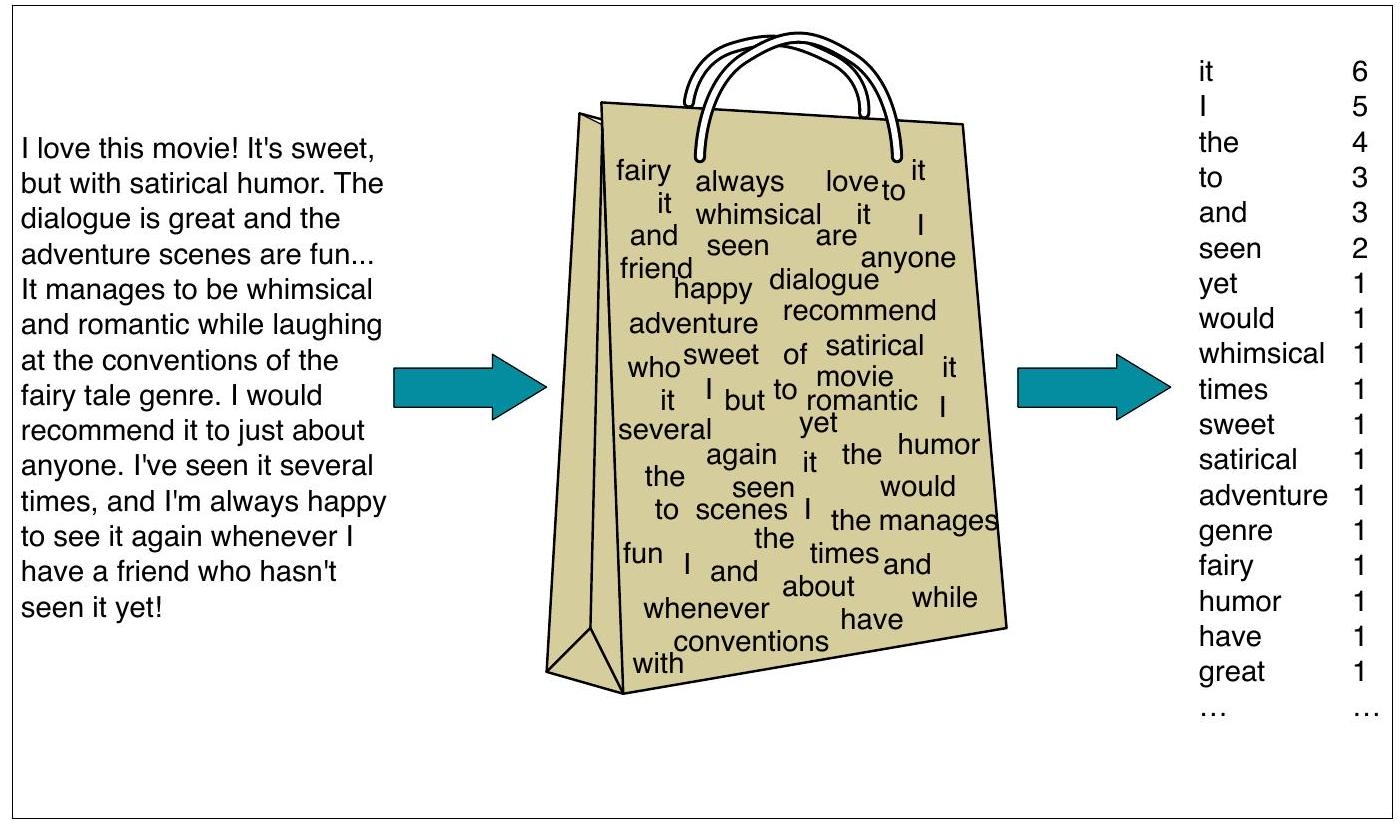
\includegraphics[max width=\textwidth, center]{2025_03_24_4f41283092a9d1f7a40eg-066}

Figure 4.1 Intuition of the multinomial naive Bayes classifier applied to a movie review. The position of the words is ignored (the bag-of-words assumption) and we make use of the frequency of each word.

Naive Bayes is a probabilistic classifier, meaning that for a document $d$, out of all classes $c \in C$ the classifier returns the class $\hat{c}$ which has the maximum posterior \^{} probability given the document. In Eq. 4.1 we use the hat notation ${ }^{\wedge}$ to mean "our estimate of the correct class", and we use argmax to mean an operation that selects the argument (in this case the class $c$ ) that maximizes a function (in this case the probability $P(c \mid d)$.


\begin{equation*}
\hat{c}=\underset{c \in C}{\operatorname{argmax}} P(c \mid d) \tag{4.1}
\end{equation*}


Bayesian\\
inference This idea of Bayesian inference has been known since the work of Bayes (1763), and was first applied to text classification by Mosteller and Wallace (1964). The intuition of Bayesian classification is to use Bayes' rule to transform Eq. 4.1 into other probabilities that have some useful properties. Bayes' rule is presented in Eq. 4.2; it gives us a way to break down any conditional probability $P(x \mid y)$ into three other probabilities:


\begin{equation*}
P(x \mid y)=\frac{P(y \mid x) P(x)}{P(y)} \tag{4.2}
\end{equation*}


We can then substitute Eq. 4.2 into Eq. 4.1 to get Eq. 4.3:


\begin{equation*}
\hat{c}=\underset{c \in C}{\operatorname{argmax}} P(c \mid d)=\underset{c \in C}{\operatorname{argmax}} \frac{P(d \mid c) P(c)}{P(d)} \tag{4.3}
\end{equation*}


We can conveniently simplify Eq. 4.3 by dropping the denominator $P(d)$. This is possible because we will be computing $\frac{P(d \mid c) P(c)}{P(d)}$ for each possible class. But $P(d)$ doesn't change for each class; we are always asking about the most likely class for the same document $d$, which must have the same probability $P(d)$. Thus, we can choose the class that maximizes this simpler formula:


\begin{equation*}
\hat{c}=\underset{c \in C}{\operatorname{argmax}} P(c \mid d)=\underset{c \in C}{\operatorname{argmax}} P(d \mid c) P(c) \tag{4.4}
\end{equation*}


We call Naive Bayes a generative model because we can read Eq. 4.4 as stating a kind of implicit assumption about how a document is generated: first a class is sampled from $P(c)$, and then the words are generated by sampling from $P(d \mid c)$. (In fact we could imagine generating artificial documents, or at least their word counts, by following this process). We'll say more about this intuition of generative models in Chapter 5.

To return to classification: we compute the most probable class $\hat{c}$ given some document $d$ by choosing the class which has the highest product of two probabilities: the prior probability of the class $P(c)$ and the likelihood of the document $P(d \mid c)$ :

$$
\hat{c}=\underset{c \in C}{\operatorname{argmax}} \overbrace{P(d \mid c)}^{\text {likelihood }} \overbrace{P(c)}^{\text {prior }}
$$

Without loss of generality, we can represent a document $d$ as a set of features $f_{1}, f_{2}, \ldots, f_{n}$ :


\begin{equation*}
\hat{c}=\underset{c \in C}{\operatorname{argmax}} \overbrace{P\left(f_{1}, f_{2}, \ldots ., f_{n} \mid c\right)}^{\text {likelihood }} \overbrace{P(c)}^{\text {prior }} \tag{4.6}
\end{equation*}


Unfortunately, Eq. 4.6 is still too hard to compute directly: without some simplifying assumptions, estimating the probability of every possible combination of features (for example, every possible set of words and positions) would require huge numbers of parameters and impossibly large training sets. Naive Bayes classifiers therefore make two simplifying assumptions.

The first is the bag-of-words assumption discussed intuitively above: we assume position doesn't matter, and that the word "love" has the same effect on classification whether it occurs as the 1st, 20th, or last word in the document. Thus we assume that the features $f_{1}, f_{2}, \ldots, f_{n}$ only encode word identity and not position.

The second is commonly called the naive Bayes assumption: this is the conditional independence assumption that the probabilities $P\left(f_{i} \mid c\right)$ are independent given the class $c$ and hence can be 'naively' multiplied as follows:


\begin{equation*}
P\left(f_{1}, f_{2}, \ldots, f_{n} \mid c\right)=P\left(f_{1} \mid c\right) \cdot P\left(f_{2} \mid c\right) \cdot \ldots \cdot P\left(f_{n} \mid c\right) \tag{4.7}
\end{equation*}


The final equation for the class chosen by a naive Bayes classifier is thus:


\begin{equation*}
c_{N B}=\underset{c \in C}{\operatorname{argmax}} P(c) \prod_{f \in F} P(f \mid c) \tag{4.8}
\end{equation*}


To apply the naive Bayes classifier to text, we will use each word in the documents as a feature, as suggested above, and we consider each of the words in the document by walking an index through every word position in the document:


\begin{align*}
\text { positions } & \leftarrow \text { all word positions in test document } \\
c_{N B} & =\underset{c \in C}{\operatorname{argmax}} P(c) \prod_{i \in \text { positions }} P\left(w_{i} \mid c\right) \tag{4.9}
\end{align*}


Naive Bayes calculations, like calculations for language modeling, are done in log space, to avoid underflow and increase speed. Thus Eq. 4.9 is generally instead expressed ${ }^{1}$ as


\begin{equation*}
c_{N B}=\underset{c \in C}{\operatorname{argmax}} \log P(c)+\sum_{i \in \text { positions }} \log P\left(w_{i} \mid c\right) \tag{4.10}
\end{equation*}


By considering features in log space, Eq. 4.10 computes the predicted class as a linear function of input features. Classifiers that use a linear combination of the inputs to make a classification decision -like naive Bayes and also logistic regressionlinear are called linear classifiers.

\subsection*{4.2 Training the Naive Bayes Classifier}
How can we learn the probabilities $P(c)$ and $P\left(f_{i} \mid c\right)$ ? Let's first consider the maximum likelihood estimate. We'll simply use the frequencies in the data. For the class prior $P(c)$ we ask what percentage of the documents in our training set are in each class $c$. Let $N_{c}$ be the number of documents in our training data with class $c$ and $N_{d o c}$ be the total number of documents. Then:


\begin{equation*}
\hat{P}(c)=\frac{N_{c}}{N_{d o c}} \tag{4.11}
\end{equation*}


To learn the probability $P\left(f_{i} \mid c\right)$, we'll assume a feature is just the existence of a word in the document's bag of words, and so we'll want $P\left(w_{i} \mid c\right)$, which we compute as the fraction of times the word $w_{i}$ appears among all words in all documents of topic $c$. We first concatenate all documents with category $c$ into one big "category $c$ " text. Then we use the frequency of $w_{i}$ in this concatenated document to give a maximum likelihood estimate of the probability:


\begin{equation*}
\hat{P}\left(w_{i} \mid c\right)=\frac{\operatorname{count}\left(w_{i}, c\right)}{\sum_{w \in V} \operatorname{count}(w, c)} \tag{4.12}
\end{equation*}


Here the vocabulary V consists of the union of all the word types in all classes, not just the words in one class $c$.

There is a problem, however, with maximum likelihood training. Imagine we are trying to estimate the likelihood of the word "fantastic" given class positive, but suppose there are no training documents that both contain the word "fantastic" and are classified as positive. Perhaps the word "fantastic" happens to occur (sarcastically?) in the class negative. In such a case the probability for this feature will be zero:


\begin{equation*}
\hat{P}(\text { "fantastic" } \mid \text { positive })=\frac{\operatorname{count}(\text { "fantastic", positive })}{\sum_{w \in V} \operatorname{count}(w, \text { positive })}=0 \tag{4.13}
\end{equation*}


\footnotetext{1 In practice throughout this book, we'll use $\log$ to mean natural $\log (\ln )$ when the base is not specified.
}But since naive Bayes naively multiplies all the feature likelihoods together, zero probabilities in the likelihood term for any class will cause the probability of the class to be zero, no matter the other evidence!

The simplest solution is the add-one (Laplace) smoothing introduced in Chapter 3. While Laplace smoothing is usually replaced by more sophisticated smoothing algorithms in language modeling, it is commonly used in naive Bayes text categorization:


\begin{equation*}
\hat{P}\left(w_{i} \mid c\right)=\frac{\operatorname{count}\left(w_{i}, c\right)+1}{\sum_{w \in V}(\operatorname{count}(w, c)+1)}=\frac{\operatorname{count}\left(w_{i}, c\right)+1}{\left(\sum_{w \in V} \operatorname{count}(w, c)\right)+|V|} \tag{4.14}
\end{equation*}


Note once again that it is crucial that the vocabulary V consists of the union of all the word types in all classes, not just the words in one class $c$ (try to convince yourself why this must be true; see the exercise at the end of the chapter).

What do we do about words that occur in our test data but are not in our vocabulary at all because they did not occur in any training document in any class? The\\
unknown word\\
stop words solution for such unknown words is to ignore them-remove them from the test document and not include any probability for them at all.

Finally, some systems choose to completely ignore another class of words: stop words, very frequent words like the and $a$. This can be done by sorting the vocabulary by frequency in the training set, and defining the top 10-100 vocabulary entries as stop words, or alternatively by using one of the many predefined stop word lists available online. Then each instance of these stop words is simply removed from both training and test documents as if it had never occurred. In most text classification applications, however, using a stop word list doesn't improve performance, and so it is more common to make use of the entire vocabulary and not use a stop word list.

Fig. 4.2 shows the final algorithm.

\subsection*{4.3 Worked example}
Let's walk through an example of training and testing naive Bayes with add-one smoothing. We'll use a sentiment analysis domain with the two classes positive $(+)$ and negative ( - ), and take the following miniature training and test documents simplified from actual movie reviews.

\begin{center}
\begin{tabular}{lll}
\hline
\multicolumn{2}{c}{Cat} & \multicolumn{1}{c}{Documents} \\
\hline
Training & - & just plain boring \\
 & - & entirely predictable and lacks energy \\
 & + & no surprises and very few laughs \\
 & + & very powerful \\
 & + & the most fun film of the summer \\
\hline
Test & $?$ & predictable with no fun \\
\hline
\end{tabular}
\end{center}

The prior $P(c)$ for the two classes is computed via Eq. 4.11 as $\frac{N_{c}}{N_{d o c}}$ :

$$
P(-)=\frac{3}{5} \quad P(+)=\frac{2}{5}
$$

The word with doesn't occur in the training set, so we drop it completely (as mentioned above, we don't use unknown word models for naive Bayes). The likelihoods from the training set for the remaining three words "predictable", "no", and

\begin{verbatim}
function Train Naive Bayes(D, C) returns $V, \log P(c), \log P(w \mid c)$
for each class $c \in C \quad$ \# Calculate $P(c)$ terms
    $\mathrm{N}_{d o c}=$ number of documents in D
    $\mathrm{N}_{c}=$ number of documents from D in class c
    logprior $[\mathrm{c}] \leftarrow \log \frac{N_{c}}{N_{d o c}}$
    $V \leftarrow$ vocabulary of D
    bigdoc $[c] \leftarrow \operatorname{append}(\mathrm{d})$ for $\mathrm{d} \in \mathrm{D}$ with class $c$
    for each word $w$ in V \# Calculate $P(w \mid c)$ terms
        count $(w, c) \leftarrow \#$ of occurrences of $w$ in bigdoc $[c]$
        loglikelihood $[\mathrm{w}, \mathrm{c}] \leftarrow \log \frac{\operatorname{count}(w, c)+1}{\sum_{w^{\prime} \text { in } V}\left(\operatorname{count}\left(w^{\prime}, c\right)+1\right)}$
$\mathbf{r n}$ logprior, loglikelihood, $V$
function Test Naive Bayes(testdoc, logprior, loglikelihood, $\mathrm{C}, \mathrm{V}$ ) returns best $c$
for each class $c \in C$
    sum $[c] \leftarrow$ logprior $[c]$
    for each position $i$ in testdoc
        word $\leftarrow$ testdoc[i]
        if word $\in V$
        sum $[c] \leftarrow$ sum $[c]+$ loglikelihood $[$ word, $c]$
return $\operatorname{argmax}_{c} \operatorname{sum}[c]$
\end{verbatim}

Figure 4.2 The naive Bayes algorithm, using add-1 smoothing. To use add- $\alpha$ smoothing instead, change the +1 to $+\alpha$ for loglikelihood counts in training.\\
"fun", are as follows, from Eq. 4.14 (computing the probabilities for the remainder of the words in the training set is left as an exercise for the reader):

$$
\begin{aligned}
& P(\text { "predictable" } \mid-)=\frac{1+1}{14+20} \quad P(\text { "predictable" } \mid+)=\frac{0+1}{9+20} \\
& P(" \mathrm{no"} \mid-)=\frac{1+1}{14+20} \quad P(\text { "no" } \mid+)=\frac{0+1}{9+20} \\
& P(\text { "fun" } \mid-)=\frac{0+1}{14+20} \quad P(\text { "fun" } \mid+)=\frac{1+1}{9+20}
\end{aligned}
$$

For the test sentence $\mathrm{S}=$ "predictable with no fun", after removing the word 'with', the chosen class, via Eq. 4.9, is therefore computed as follows:

$$
\begin{aligned}
& P(-) P(S \mid-)=\frac{3}{5} \times \frac{2 \times 2 \times 1}{34^{3}}=6.1 \times 10^{-5} \\
& P(+) P(S \mid+)=\frac{2}{5} \times \frac{1 \times 1 \times 2}{29^{3}}=3.2 \times 10^{-5}
\end{aligned}
$$

The model thus predicts the class negative for the test sentence.

\subsection*{4.4 Optimizing for Sentiment Analysis}
While standard naive Bayes text classification can work well for sentiment analysis, some small changes are generally employed that improve performance.

First, for sentiment classification and a number of other text classification tasks, whether a word occurs or not seems to matter more than its frequency. Thus it often improves performance to clip the word counts in each document at 1 (see the end of the chapter for pointers to these results). This variant is called binary multinomial naive Bayes or binary naive Bayes. The variant uses the same algorithm as in Fig. 4.2 except that for each document we remove all duplicate words before concatenating them into the single big document during training and we also remove duplicate words from test documents. Fig. 4.3 shows an example in which a set of four documents (shortened and text-normalized for this example) are remapped to binary, with the modified counts shown in the table on the right. The example is worked without add-1 smoothing to make the differences clearer. Note that the results counts need not be 1 ; the word great has a count of 2 even for binary naive Bayes, because it appears in multiple documents.

\begin{center}
\begin{tabular}{|c|c|c|c|c|c|}
\hline
\multirow[b]{2}{*}{Four original documents:} &  & \multicolumn{2}{|l|}{NB Counts} & \multicolumn{2}{|l|}{Binary Counts} \\
\hline
 &  & + & - & + & - \\
\hline
- it was pathetic the worst part was the & and & 2 & 0 & 1 & 0 \\
\hline
boxing scenes & boxing & 0 & 1 & 0 & 1 \\
\hline
 & film & 1 & 0 & 1 & 0 \\
\hline
- no plot twists or great scenes & great & 3 & 1 & 2 & 1 \\
\hline
+ and satire and great plot twists & it & 0 & 1 & 0 & 1 \\
\hline
+ great scenes great film & no & 0 & 1 & 0 & 1 \\
\hline
 & or & 0 & 1 & 0 & 1 \\
\hline
After per-document binarization: & part & 0 & 1 & 0 & 1 \\
\hline
- it was pathetic the worst part boxing & pathetic & 0 & 1 & 0 & 1 \\
\hline
scenes & plot & 1 & 1 & , & 1 \\
\hline
 & satire & 1 & 0 & 1 & 0 \\
\hline
- no plot twists or great scenes & scenes & 1 & 2 & 1 & 2 \\
\hline
+ and satire great plot twists & the & 0 & 2 & 0 & , \\
\hline
+ great scenes film & twists & 1 & 1 & 1 & 1 \\
\hline
 & was & 0 & 2 & 0 & 1 \\
\hline
 & worst & 0 & 1 & 0 & 1 \\
\hline
\end{tabular}
\end{center}

Figure 4.3 An example of binarization for the binary naive Bayes algorithm.\\
A second important addition commonly made when doing text classification for sentiment is to deal with negation. Consider the difference between I really like this movie (positive) and I didn't like this movie (negative). The negation expressed by didn't completely alters the inferences we draw from the predicate like. Similarly, negation can modify a negative word to produce a positive review (don't dismiss this film, doesn't let us get bored).

A very simple baseline that is commonly used in sentiment analysis to deal with negation is the following: during text normalization, prepend the prefix $N O T_{-}$to every word after a token of logical negation ( $n$ 't, not, no, never) until the next punctuation mark. Thus the phrase

\begin{verbatim}
didn't like this movie , but I
becomes
\end{verbatim}

\begin{verbatim}
didn't NOT_like NOT_this NOT_movie , but I
\end{verbatim}

\begin{verbatim}
didn't NOT_like NOT_this NOT_movie , but I
\end{verbatim}

Newly formed 'words' like NOT\_like, NOT\_recommend will thus occur more often in negative document and act as cues for negative sentiment, while words like NOT\_bored, NOT\_dismiss will acquire positive associations. Syntactic parsing (Chapter 18) can be used deal more accurately with the scope relationship between\\
sentiment\\
these negation words and the predicates they modify, but this simple baseline works quite well in practice.

Finally, in some situations we might have insufficient labeled training data to train accurate naive Bayes classifiers using all words in the training set to estimate positive and negative sentiment. In such cases we can instead derive the positive and negative word features from sentiment lexicons, lists of words that are preannotated with positive or negative sentiment. Four popular lexicons are the General Inquirer (Stone et al., 1966), LIWC (Pennebaker et al., 2007), the opinion lexicon of Hu and Liu (2004a) and the MPQA Subjectivity Lexicon (Wilson et al., 2005).

For example the MPQA subjectivity lexicon has 6885 words each marked for whether it is strongly or weakly biased positive or negative. Some examples:

\begin{itemize}
  \item : admirable, beautiful, confident, dazzling, ecstatic, favor, glee, great
\end{itemize}

\begin{itemize}
  \item : awful, bad, bias, catastrophe, cheat, deny, envious, foul, harsh, hate
\end{itemize}

A common way to use lexicons in a naive Bayes classifier is to add a feature that is counted whenever a word from that lexicon occurs. Thus we might add a feature called 'this word occurs in the positive lexicon', and treat all instances of words in the lexicon as counts for that one feature, instead of counting each word separately. Similarly, we might add as a second feature 'this word occurs in the negative lexicon' of words in the negative lexicon. If we have lots of training data, and if the test data matches the training data, using just two features won't work as well as using all the words. But when training data is sparse or not representative of the test set, using dense lexicon features instead of sparse individual-word features may generalize better.

We'll return to this use of lexicons in Chapter 22, showing how these lexicons can be learned automatically, and how they can be applied to many other tasks beyond sentiment classification.

\subsection*{4.5 Naive Bayes for other text classification tasks}
In the previous section we pointed out that naive Bayes doesn't require that our classifier use all the words in the training data as features. In fact features in naive Bayes can express any property of the input text we want.

Consider the task of spam detection, deciding if a particular piece of email is an example of spam (unsolicited bulk email)—one of the first applications of naive Bayes to text classification (Sahami et al., 1998).

A common solution here, rather than using all the words as individual features, is to predefine likely sets of words or phrases as features, combined with features that are not purely linguistic. For example the open-source SpamAssassin tool ${ }^{2}$ predefines features like the phrase "one hundred percent guaranteed", or the feature mentions millions of dollars, which is a regular expression that matches suspiciously large sums of money. But it also includes features like HTML has a low ratio of text to image area, that aren't purely linguistic and might require some sophisticated computation, or totally non-linguistic features about, say, the path that the email took to arrive. More sample SpamAssassin features:

\begin{itemize}
  \item Email subject line is all capital letters
  \item Contains phrases of urgency like "urgent reply"
\end{itemize}

\footnotetext{2 \href{https://spamassassin.apache.org}{https://spamassassin.apache.org}
}\begin{itemize}
  \item Email subject line contains "online pharmaceutical"
  \item HTML has unbalanced "head" tags
  \item Claims you can be removed from the list\\
language id\\
For other tasks, like language id-determining what language a given piece of text is written in-the most effective naive Bayes features are not words at all, but character n-grams, 2-grams ('zw') 3-grams ('nya', ' Vo'), or 4-grams ('ie z', 'thei'), or, even simpler byte n-grams, where instead of using the multibyte Unicode character representations called codepoints, we just pretend everything is a string of raw bytes. Because spaces count as a byte, byte n-grams can model statistics about the beginning or ending of words. A widely used naive Bayes system, \href{http://langid.py}{langid.py} (Lui and Baldwin, 2012) begins with all possible n-grams of lengths 1-4, using feature selection to winnow down to the most informative 7000 final features.
\end{itemize}

Language ID systems are trained on multilingual text, such as Wikipedia (Wikipedia text in 68 different languages was used in (Lui and Baldwin, 2011)), or newswire. To make sure that this multilingual text correctly reflects different regions, dialects, and socioeconomic classes, systems also add Twitter text in many languages geotagged to many regions (important for getting world English dialects from countries with large Anglophone populations like Nigeria or India), Bible and Quran translations, slang websites like Urban Dictionary, corpora of African American Vernacular English (Blodgett et al., 2016), and so on (Jurgens et al., 2017).

\subsection*{4.6 Naive Bayes as a Language Model}
As we saw in the previous section, naive Bayes classifiers can use any sort of feature: dictionaries, URLs, email addresses, network features, phrases, and so on. But if, as in Section 4.3, we use only individual word features, and we use all of the words in the text (not a subset), then naive Bayes has an important similarity to language modeling. Specifically, a naive Bayes model can be viewed as a set of class-specific unigram language models, in which the model for each class instantiates a unigram language model.

Since the likelihood features from the naive Bayes model assign a probability to each word $P(\operatorname{word} \mid c)$, the model also assigns a probability to each sentence:


\begin{equation*}
P(s \mid c)=\prod_{i \in \text { positions }} P\left(w_{i} \mid c\right) \tag{4.15}
\end{equation*}


Thus consider a naive Bayes model with the classes positive (+) and negative (-) and the following model parameters:

\begin{center}
\begin{tabular}{lll}
$\mathbf{w}$ & $\mathbf{P}(\mathbf{w} \mid+)$ & $\mathbf{P}(\mathbf{w} \mid-)$ \\
\hline
I & 0.1 & 0.2 \\
love & 0.1 & 0.001 \\
this & 0.01 & 0.01 \\
fun & 0.05 & 0.005 \\
film & 0.1 & 0.1 \\
$\ldots$ & $\ldots$ & $\ldots$ \\
\hline
\end{tabular}
\end{center}

Each of the two columns above instantiates a language model that can assign a probability to the sentence "I love this fun film":\\
$P($ "I love this fun film" $\mid+)=0.1 \times 0.1 \times 0.01 \times 0.05 \times 0.1=5 \times 10^{-7}$\\
$P($ "I love this fun film" $\mid-)=0.2 \times 0.001 \times 0.01 \times 0.005 \times 0.1=1.0 \times 10^{-9}$\\
As it happens, the positive model assigns a higher probability to the sentence: $P(s \mid p o s)>P(s \mid n e g)$. Note that this is just the likelihood part of the naive Bayes model; once we multiply in the prior a full naive Bayes model might well make a different classification decision.

\subsection*{4.7 Evaluation: Precision, Recall, F-measure}
To introduce the methods for evaluating text classification, let's first consider some simple binary detection tasks. For example, in spam detection, our goal is to label every text as being in the spam category ("positive") or not in the spam category ("negative"). For each item (email document) we therefore need to know whether our system called it spam or not. We also need to know whether the email is actually spam or not, i.e. the human-defined labels for each document that we are trying to match. We will refer to these human labels as the gold labels.

Or imagine you're the CEO of the Delicious Pie Company and you need to know what people are saying about your pies on social media, so you build a system that detects tweets concerning Delicious Pie. Here the positive class is tweets about Delicious Pie and the negative class is all other tweets.

In both cases, we need a metric for knowing how well our spam detector (or pie-tweet-detector) is doing. To evaluate any system for detecting things, we start by building a confusion matrix like the one shown in Fig. 4.4. A confusion matrix is a table for visualizing how an algorithm performs with respect to the human gold labels, using two dimensions (system output and gold labels), and each cell labeling a set of possible outcomes. In the spam detection case, for example, true positives are documents that are indeed spam (indicated by human-created gold labels) that our system correctly said were spam. False negatives are documents that are indeed spam but our system incorrectly labeled as non-spam.

To the bottom right of the table is the equation for accuracy, which asks what percentage of all the observations (for the spam or pie examples that means all emails or tweets) our system labeled correctly. Although accuracy might seem a natural metric, we generally don't use it for text classification tasks. That's because accuracy doesn't work well when the classes are unbalanced (as indeed they are with spam, which is a large majority of email, or with tweets, which are mainly not about pie).

To make this more explicit, imagine that we looked at a million tweets, and let's say that only 100 of them are discussing their love (or hatred) for our pie, while the other 999,900 are tweets about something completely unrelated. Imagine a simple classifier that stupidly classified every tweet as "not about pie". This classifier would have 999,900 true negatives and only 100 false negatives for an accuracy of $999,900 / 1,000,000$ or $99.99 \%$ ! What an amazing accuracy level! Surely we should be happy with this classifier? But of course this fabulous 'no pie' classifier would be completely useless, since it wouldn't find a single one of the customer comments we are looking for. In other words, accuracy is not a good metric when the goal is to discover something that is rare, or at least not completely balanced in frequency, which is a very common situation in the world.\\
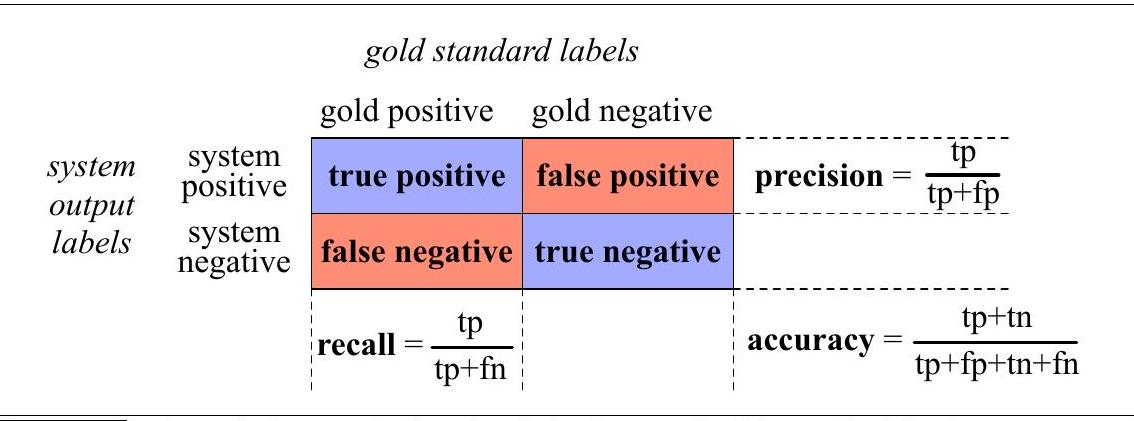
\includegraphics[max width=\textwidth, center]{2025_03_24_4f41283092a9d1f7a40eg-075}

Figure 4.4 A confusion matrix for visualizing how well a binary classification system performs against gold standard labels.

That's why instead of accuracy we generally turn to two other metrics shown in

Fig. 4.4: precision and recall. Precision measures the percentage of the items that the system detected (i.e., the system labeled as positive) that are in fact positive (i.e., are positive according to the human gold labels). Precision is defined as

$$
\text { Precision }=\frac{\text { true positives }}{\text { true positives }+ \text { false positives }}
$$

Recall measures the percentage of items actually present in the input that were correctly identified by the system. Recall is defined as

$$
\text { Recall }=\frac{\text { true positives }}{\text { true positives }+ \text { false negatives }}
$$

Precision and recall will help solve the problem with the useless "nothing is pie" classifier. This classifier, despite having a fabulous accuracy of $99.99 \%$, has a terrible recall of 0 (since there are no true positives, and 100 false negatives, the recall is $0 / 100$ ). You should convince yourself that the precision at finding relevant tweets is equally problematic. Thus precision and recall, unlike accuracy, emphasize true positives: finding the things that we are supposed to be looking for.

There are many ways to define a single metric that incorporates aspects of both precision and recall. The simplest of these combinations is the F-measure (van Rijsbergen, 1975), defined as:

$$
F_{\beta}=\frac{\left(\beta^{2}+1\right) P R}{\beta^{2} P+R}
$$

The $\beta$ parameter differentially weights the importance of recall and precision, based perhaps on the needs of an application. Values of $\beta>1$ favor recall, while values of $\beta<1$ favor precision. When $\beta=1$, precision and recall are equally balanced; this is the most frequently used metric, and is called $F_{\beta=1}$ or just $F_{1}$ :


\begin{equation*}
\mathrm{F}_{1}=\frac{2 P R}{P+R} \tag{4.16}
\end{equation*}


F-measure comes from a weighted harmonic mean of precision and recall. The harmonic mean of a set of numbers is the reciprocal of the arithmetic mean of reciprocals:


\begin{equation*}
\operatorname{HarmonicMean}\left(a_{1}, a_{2}, a_{3}, a_{4}, \ldots, a_{n}\right)=\frac{n}{\frac{1}{a_{1}}+\frac{1}{a_{2}}+\frac{1}{a_{3}}+\ldots+\frac{1}{a_{n}}} \tag{4.17}
\end{equation*}


and hence F-measure is


\begin{equation*}
F=\frac{1}{\alpha \frac{1}{P}+(1-\alpha) \frac{1}{R}} \quad \text { or }\left(\text { with } \beta^{2}=\frac{1-\alpha}{\alpha}\right) \quad F=\frac{\left(\beta^{2}+1\right) P R}{\beta^{2} P+R} \tag{4.18}
\end{equation*}


Harmonic mean is used because the harmonic mean of two values is closer to the minimum of the two values than the arithmetic mean is. Thus it weighs the lower of the two numbers more heavily, which is more conservative in this situation.

\subsection*{4.7.1 Evaluating with more than two classes}
Up to now we have been describing text classification tasks with only two classes. But lots of classification tasks in language processing have more than two classes. For sentiment analysis we generally have 3 classes (positive, negative, neutral) and even more classes are common for tasks like part-of-speech tagging, word sense disambiguation, semantic role labeling, emotion detection, and so on. Luckily the naive Bayes algorithm is already a multi-class classification algorithm.\\
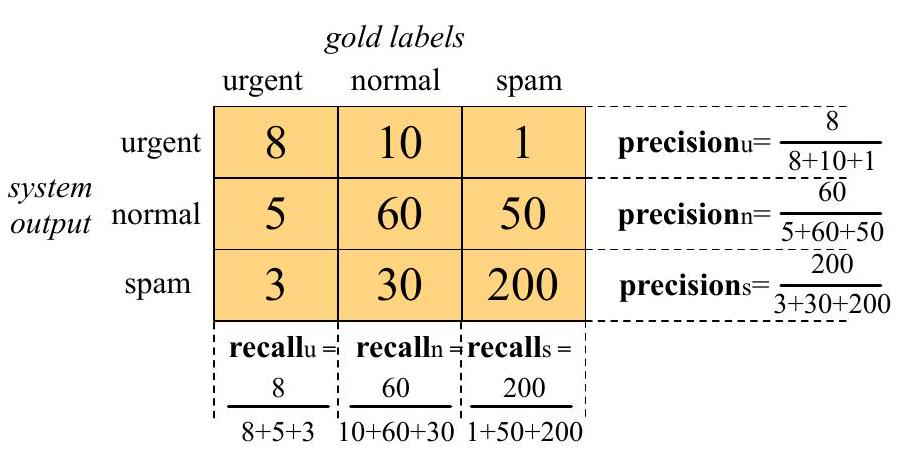
\includegraphics[max width=\textwidth, center]{2025_03_24_4f41283092a9d1f7a40eg-076}

Figure 4.5 Confusion matrix for a three-class categorization task, showing for each pair of classes $\left(c_{1}, c_{2}\right)$, how many documents from $c_{1}$ were (in)correctly assigned to $c_{2}$.

But we'll need to slightly modify our definitions of precision and recall. Consider the sample confusion matrix for a hypothetical 3-way one-of email categorization decision (urgent, normal, spam) shown in Fig. 4.5. The matrix shows, for example, that the system mistakenly labeled one spam document as urgent, and we have shown how to compute a distinct precision and recall value for each class. In order to derive a single metric that tells us how well the system is doing, we can combine these values in two ways. In macroaveraging, we compute the performance for each class, and then average over classes. In microaveraging, we collect the decisions for all classes into a single confusion matrix, and then compute precision and recall from that table. Fig. 4.6 shows the confusion matrix for each class separately, and shows the computation of microaveraged and macroaveraged precision.

As the figure shows, a microaverage is dominated by the more frequent class (in this case spam), since the counts are pooled. The macroaverage better reflects the statistics of the smaller classes, and so is more appropriate when performance on all the classes is equally important.\\
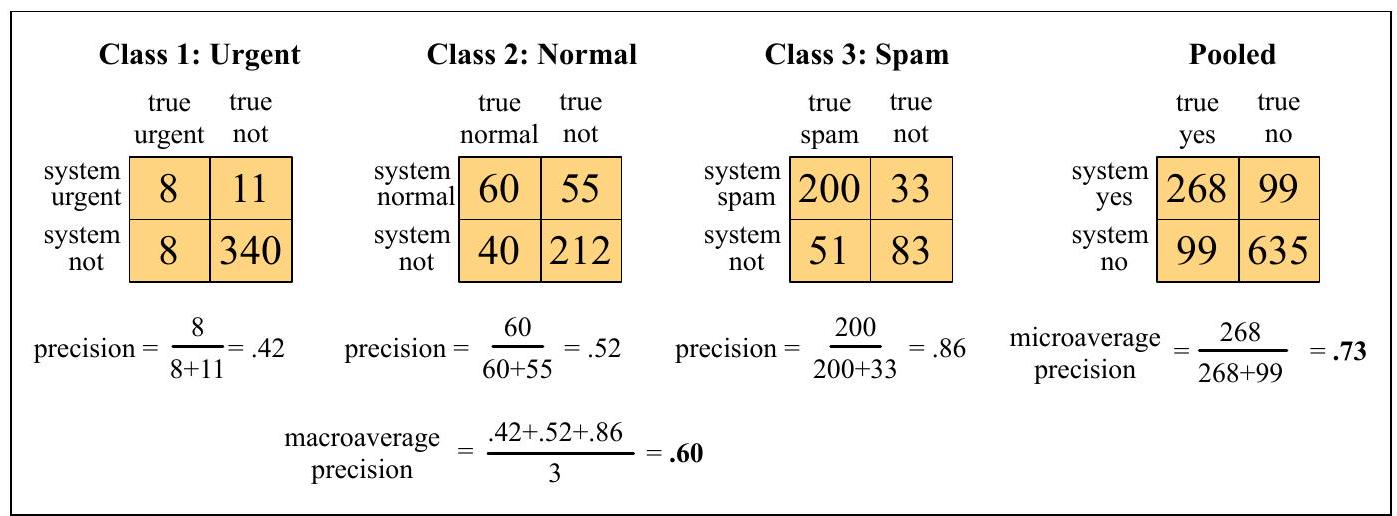
\includegraphics[max width=\textwidth, center]{2025_03_24_4f41283092a9d1f7a40eg-077}

Figure 4.6 Separate confusion matrices for the 3 classes from the previous figure, showing the pooled confusion matrix and the microaveraged and macroaveraged precision.

\subsection*{4.8 Test sets and Cross-validation}
$\underset{\substack{\text { deeselopmentet } \\ \text { dessest }}}{\text { det }}$\\
cross-validation

The training and testing procedure for text classification follows what we saw with language modeling (Section 3.2): we use the training set to train the model, then use the development test set (also called a devset) to perhaps tune some parameters, and in general decide what the best model is. Once we come up with what we think is the best model, we run it on the (hitherto unseen) test set to report its performance.

While the use of a devset avoids overfitting the test set, having a fixed training set, devset, and test set creates another problem: in order to save lots of data for training, the test set (or devset) might not be large enough to be representative. Wouldn't it be better if we could somehow use all our data for training and still use all our data for test? We can do this by cross-validation.

In cross-validation, we choose a number $k$, and partition our data into $k$ disjoint\\
folds subsets called folds. Now we choose one of those $k$ folds as a test set, train our classifier on the remaining $k-1$ folds, and then compute the error rate on the test set. Then we repeat with another fold as the test set, again training on the other $k-1$ folds. We do this sampling process $k$ times and average the test set error rate from these $k$ runs to get an average error rate. If we choose $k=10$, we would train 10 different models (each on $90 \%$ of our data), test the model 10 times, and average these 10 values. This is called $\mathbf{1 0}$-fold cross-validation.

The only problem with cross-validation is that because all the data is used for testing, we need the whole corpus to be blind; we can't examine any of the data to suggest possible features and in general see what's going on, because we'd be peeking at the test set, and such cheating would cause us to overestimate the performance of our system. However, looking at the corpus to understand what's going on is important in designing NLP systems! What to do? For this reason, it is common to create a fixed training set and test set, then do 10 -fold cross-validation inside the training set, but compute error rate the normal way in the test set, as shown in Fig. 4.7.\\
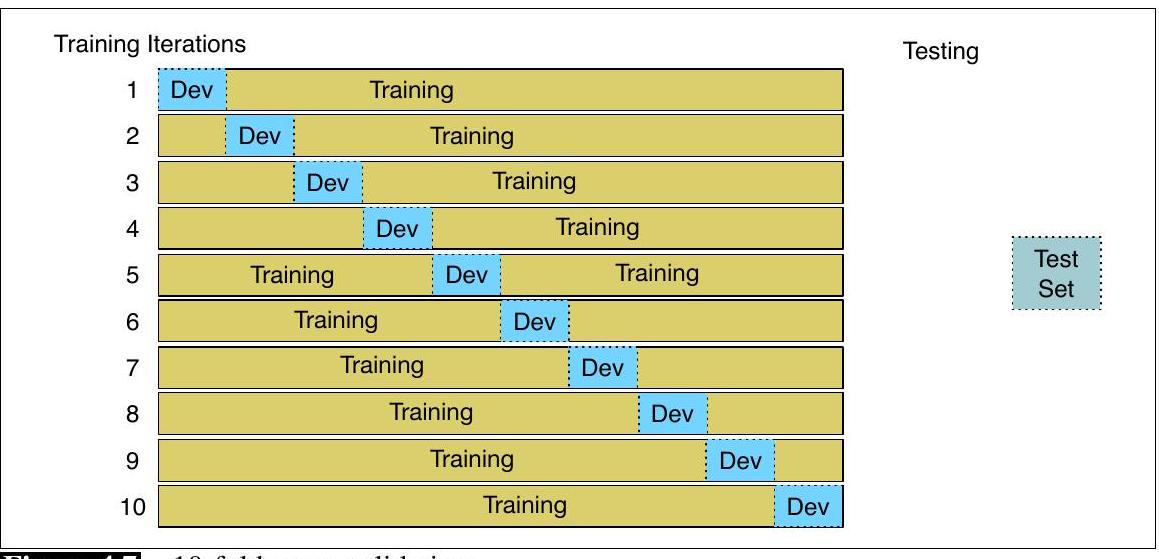
\includegraphics[max width=\textwidth, center]{2025_03_24_4f41283092a9d1f7a40eg-078}

Figure 4.710 -fold cross-validation

\subsection*{4.9 Statistical Significance Testing}
In building systems we often need to compare the performance of two systems. How can we know if the new system we just built is better than our old one? Or better than some other system described in the literature? This is the domain of statistical hypothesis testing, and in this section we introduce tests for statistical significance for NLP classifiers, drawing especially on the work of Dror et al. (2020) and BergKirkpatrick et al. (2012).

Suppose we're comparing the performance of classifiers $A$ and $B$ on a metric $M$ such as $\mathrm{F}_{1}$, or accuracy. Perhaps we want to know if our logistic regression sentiment classifier $A$ (Chapter 5) gets a higher $\mathrm{F}_{1}$ score than our naive Bayes sentiment classifier $B$ on a particular test set $x$. Let's call $M(A, x)$ the score that system $A$ gets on test set $x$, and $\delta(x)$ the performance difference between $A$ and $B$ on $x$ :


\begin{equation*}
\delta(x)=M(A, x)-M(B, x) \tag{4.19}
\end{equation*}


We would like to know if $\delta(x)>0$, meaning that our logistic regression classifier has a higher $\mathrm{F}_{1}$ than our naive Bayes classifier on $x . \delta(x)$ is called the effect size; a bigger $\delta$ means that $A$ seems to be way better than $B$; a small $\delta$ means $A$ seems to be only a little better.

Why don't we just check if $\delta(x)$ is positive? Suppose we do, and we find that the $\mathrm{F}_{1}$ score of $A$ is higher than $B$ 's by .04 . Can we be certain that $A$ is better? We cannot! That's because $A$ might just be accidentally better than $B$ on this particular $x$. We need something more: we want to know if $A$ 's superiority over $B$ is likely to hold again if we checked another test set $x^{\prime}$, or under some other set of circumstances.

In the paradigm of statistical hypothesis testing, we test this by formalizing two hypotheses.


\begin{align*}
& H_{0}: \delta(x) \leq 0 \\
& H_{1}: \delta(x)>0 \tag{4.20}
\end{align*}


The hypothesis $H_{0}$, called the null hypothesis, supposes that $\delta(x)$ is actually negative or zero, meaning that $A$ is not better than $B$. We would like to know if we can confidently rule out this hypothesis, and instead support $H_{1}$, that $A$ is better.

We do this by creating a random variable $X$ ranging over all test sets. Now we ask how likely is it, if the null hypothesis $H_{0}$ was correct, that among these test sets\\
we would encounter the value of $\delta(x)$ that we found, if we repeated the experiment\\
p-value\\
statistically significant\\
approximate approximate\\
randomization a great many times. We formalize this likelihood as the p-value: the probability, assuming the null hypothesis $H_{0}$ is true, of seeing the $\delta(x)$ that we saw or one even greater


\begin{equation*}
P\left(\boldsymbol{\delta}(X) \geq \boldsymbol{\delta}(x) \mid H_{0} \text { is true }\right) \tag{4.21}
\end{equation*}


So in our example, this p-value is the probability that we would see $\delta(x)$ assuming $A$ is not better than $B$. If $\delta(x)$ is huge (let's say $A$ has a very respectable $\mathrm{F}_{1}$ of .9 and $B$ has a terrible $\mathrm{F}_{1}$ of only .2 on $x$ ), we might be surprised, since that would be extremely unlikely to occur if $H_{0}$ were in fact true, and so the p-value would be low (unlikely to have such a large $\delta$ if $A$ is in fact not better than $B$ ). But if $\delta(x)$ is very small, it might be less surprising to us even if $H_{0}$ were true and $A$ is not really better than $B$, and so the p -value would be higher.

A very small p -value means that the difference we observed is very unlikely under the null hypothesis, and we can reject the null hypothesis. What counts as very small? It is common to use values like .05 or .01 as the thresholds. A value of .01 means that if the p-value (the probability of observing the $\delta$ we saw assuming $H_{0}$ is true) is less than .01 , we reject the null hypothesis and assume that $A$ is indeed better than $B$. We say that a result (e.g., " $A$ is better than $B$ ") is statistically significant if the $\delta$ we saw has a probability that is below the threshold and we therefore reject this null hypothesis.

How do we compute this probability we need for the p-value? In NLP we generally don't use simple parametric tests like t-tests or ANOVAs that you might be familiar with. Parametric tests make assumptions about the distributions of the test statistic (such as normality) that don't generally hold in our cases. So in NLP we usually use non-parametric tests based on sampling: we artificially create many versions of the experimental setup. For example, if we had lots of different test sets $x^{\prime}$ we could just measure all the $\delta\left(x^{\prime}\right)$ for all the $x^{\prime}$. That gives us a distribution. Now we set a threshold (like .01) and if we see in this distribution that $99 \%$ or more of those deltas are smaller than the delta we observed, i.e., that p -value $(x)$-the probability of seeing a $\boldsymbol{\delta}(x)$ as big as the one we saw-is less than .01 , then we can reject the null hypothesis and agree that $\delta(x)$ was a sufficiently surprising difference and $A$ is really a better algorithm than $B$.

There are two common non-parametric tests used in NLP: approximate randomization (Noreen, 1989) and the bootstrap test. We will describe bootstrap below, showing the paired version of the test, which again is most common in NLP.\\
paired\\
bootstrap test\\
bootstrapping

Paired tests are those in which we compare two sets of observations that are aligned: each observation in one set can be paired with an observation in another. This happens naturally when we are comparing the performance of two systems on the same test set; we can pair the performance of system $A$ on an individual observation $x_{i}$ with the performance of system $B$ on the same $x_{i}$.

\subsection*{4.9.1 The Paired Bootstrap Test}
The bootstrap test (Efron and Tibshirani, 1993) can apply to any metric; from precision, recall, or F1 to the BLEU metric used in machine translation. The word bootstrapping refers to repeatedly drawing large numbers of samples with replacement (called bootstrap samples) from an original set. The intuition of the bootstrap test is that we can create many virtual test sets from an observed test set by repeatedly sampling from it. The method only makes the assumption that the sample is representative of the population.

Consider a tiny text classification example with a test set $x$ of 10 documents. The first row of Fig. 4.8 shows the results of two classifiers (A and B) on this test set. Each document is labeled by one of the four possibilities (A and B both right, both wrong, $A$ right and $B$ wrong, $A$ wrong and $B$ right). A slash through a letter (B) means that that classifier got the answer wrong. On the first document both A and $B$ get the correct class ( AB ), while on the second document $A$ got it right but $B$ got it wrong ( $\mathrm{A}, \mathrm{B}$ ). If we assume for simplicity that our metric is accuracy, $A$ has an accuracy of .70 and B of .50 , so $\delta(x)$ is .20 .

Now we create a large number $b$ (perhaps $10^{5}$ ) of virtual test sets $x^{(i)}$, each of size $n=10$. Fig. 4.8 shows a couple of examples. To create each virtual test set $x^{(i)}$, we repeatedly ( $n=10$ times) select a cell from row $x$ with replacement. For example, to create the first cell of the first virtual test set $x^{(1)}$, if we happened to randomly select the second cell of the $x$ row; we would copy the value $A B$ into our new cell, and move on to create the second cell of $x^{(1)}$, each time sampling (randomly choosing) from the original $x$ with replacement.

\begin{center}
\begin{tabular}{lccccccccccccc}
 & 1 & 2 & 3 & 4 & 5 & 6 & 7 & 8 & 9 & 10 & $\mathrm{~A} \%$ & $\mathrm{~B} \%$ & $\delta()$ \\
\hline
$x$ & AB & AB & AB & AB & AB & AB & AB & AB & AB & AB & .70 & .50 & .20 \\
$x^{(1)}$ & AB & AB & AB & AB & AB & AB & AB & AB & AB & AB & .60 & .60 & .00 \\
$x^{(2)}$ & $\mathrm{A} \not B^{\prime}$ & AB & AB & AB & AB & AB & AB & AB & AB & AB & .60 & .70 & -.10 \\
$\ldots$ &  &  &  &  &  &  &  &  &  &  &  &  &  \\
\end{tabular}
\end{center}

Now that we have the $b$ test sets, providing a sampling distribution, we can do statistics on how often $A$ has an accidental advantage. There are various ways to compute this advantage; here we follow the version laid out in Berg-Kirkpatrick et al. (2012). Assuming $H_{0}$ ( $A$ isn't better than $B$ ), we would expect that $\delta(X)$, estimated over many test sets, would be zero or negative; a much higher value would be surprising, since $H_{0}$ specifically assumes $A$ isn't better than $B$. To measure exactly how surprising our observed $\delta(x)$ is, we would in other circumstances compute the p-value by counting over many test sets how often $\delta\left(x^{(i)}\right)$ exceeds the expected zero value by $\delta(x)$ or more:

$$
\mathrm{p} \text {-value }(x)=\frac{1}{b} \sum_{i=1}^{b} \mathbb{1}\left(\delta\left(x^{(i)}\right)-\delta(x) \geq 0\right)
$$

(We use the notation $\mathbb{1}(x)$ to mean " 1 if $x$ is true, and 0 otherwise".) However, although it's generally true that the expected value of $\delta(X)$ over many test sets, (again assuming $A$ isn't better than $B$ ) is 0 , this isn't true for the bootstrapped test sets we created. That's because we didn't draw these samples from a distribution with 0 mean; we happened to create them from the original test set $x$, which happens to be biased (by .20) in favor of $A$. So to measure how surprising is our observed $\delta(x)$, we actually compute the p -value by counting over many test sets how often\\
$\delta\left(x^{(i)}\right)$ exceeds the expected value of $\delta(x)$ by $\delta(x)$ or more:


\begin{align*}
\mathrm{p} \text {-value }(x) & =\frac{1}{b} \sum_{i=1}^{b} \mathbb{1}\left(\delta\left(x^{(i)}\right)-\delta(x) \geq \delta(x)\right) \\
& =\frac{1}{b} \sum_{i=1}^{b} \mathbb{1}\left(\delta\left(x^{(i)}\right) \geq 2 \boldsymbol{\delta}(x)\right) \tag{4.22}
\end{align*}


So if for example we have 10,000 test sets $x^{(i)}$ and a threshold of .01 , and in only 47 of the test sets do we find that A is accidentally better $\delta\left(x^{(i)}\right) \geq 2 \delta(x)$, the resulting p -value of .0047 is smaller than .01 , indicating that the delta we found, $\delta(x)$ is indeed sufficiently surprising and unlikely to have happened by accident, and we can reject the null hypothesis and conclude $A$ is better than $B$.

\begin{displayquote}
function Bootstrap(test set $x$, num of samples $b$ ) returns $p$-value $(x)$\\
Calculate $\delta(x)$ \# how much better does algorithm A do than B on $x$ $s=0$\\
for $i=1$ to $b$ do\\
for $j=1$ to $n$ do \# Draw a bootstrap sample $x^{(i)}$ of size n Select a member of $x$ at random and add it to $x^{(i)}$\\
Calculate $\delta\left(x^{(i)}\right) \quad$ \# how much better does algorithm A do than B on $x^{(i)}$\\
$s \leftarrow s+1$ if $\delta\left(x^{(i)}\right) \geq 2 \delta(x)$\\
p-value $(x) \approx \frac{s}{b} \quad$ \# on what $\%$ of the b samples did algorithm A beat expectations?\\
return p-value $(x) \quad$ \# if very few did, our observed $\delta$ is probably not accidental
\end{displayquote}

Figure 4.9\\
A version of the paired bootstrap algorithm after Berg-Kirkpatrick et al. (2012).\\
The full algorithm for the bootstrap is shown in Fig. 4.9. It is given a test set $x$, a number of samples $b$, and counts the percentage of the $b$ bootstrap test sets in which $\delta\left(x^{*(i)}\right)>2 \boldsymbol{\delta}(x)$. This percentage then acts as a one-sided empirical p-value.

\subsection*{4.10 Avoiding Harms in Classification}
It is important to avoid harms that may result from classifiers, harms that exist both for naive Bayes classifiers and for the other classification algorithms we introduce in later chapters.

One class of harms is representational harms (Crawford 2017, Blodgett et al. 2020), harms caused by a system that demeans a social group, for example by perpetuating negative stereotypes about them. For example Kiritchenko and Mohammad (2018) examined the performance of 200 sentiment analysis systems on pairs of sentences that were identical except for containing either a common African American first name (like Shaniqua) or a common European American first name (like Stephanie), chosen from the Caliskan et al. (2017) study discussed in Chapter 6. They found that most systems assigned lower sentiment and more negative emotion to sentences with African American names, reflecting and perpetuating stereotypes that associate African Americans with negative emotions (Popp et al., 2003).

In other tasks classifiers may lead to both representational harms and other harms, such as silencing. For example the important text classification task of tox-\\
icity detection is the task of detecting hate speech, abuse, harassment, or other kinds of toxic language. While the goal of such classifiers is to help reduce societal harm, toxicity classifiers can themselves cause harms. For example, researchers have shown that some widely used toxicity classifiers incorrectly flag as being toxic sentences that are non-toxic but simply mention identities like women (Park et al., 2018), blind people (Hutchinson et al., 2020) or gay people (Dixon et al., 2018; Dias Oliva et al., 2021), or simply use linguistic features characteristic of varieties like African-American Vernacular English (Sap et al. 2019, Davidson et al. 2019). Such false positive errors could lead to the silencing of discourse by or about these groups.

These model problems can be caused by biases or other problems in the training data; in general, machine learning systems replicate and even amplify the biases in their training data. But these problems can also be caused by the labels (for example due to biases in the human labelers), by the resources used (like lexicons, or model components like pretrained embeddings), or even by model architecture (like what the model is trained to optimize). While the mitigation of these biases (for example by carefully considering the training data sources) is an important area of research, we currently don't have general solutions. For this reason it's important, when introducing any NLP model, to study these kinds of factors and make them clear. One way to do this is by releasing a model card (Mitchell et al., 2019) for each version of a model. A model card documents a machine learning model with information like:

\begin{itemize}
  \item training algorithms and parameters
  \item training data sources, motivation, and preprocessing
  \item evaluation data sources, motivation, and preprocessing
  \item intended use and users
  \item model performance across different demographic or other groups and environmental situations
\end{itemize}

\subsection*{4.11 Summary}
This chapter introduced the naive Bayes model for classification and applied it to the text categorization task of sentiment analysis.

\begin{itemize}
  \item Many language processing tasks can be viewed as tasks of classification.
  \item Text categorization, in which an entire text is assigned a class from a finite set, includes such tasks as sentiment analysis, spam detection, language identification, and authorship attribution.
  \item Sentiment analysis classifies a text as reflecting the positive or negative orientation (sentiment) that a writer expresses toward some object.
  \item Naive Bayes is a generative model that makes the bag-of-words assumption (position doesn't matter) and the conditional independence assumption (words are conditionally independent of each other given the class)
  \item Naive Bayes with binarized features seems to work better for many text classification tasks.
  \item Classifiers are evaluated based on precision and recall.
  \item Classifiers are trained using distinct training, dev, and test sets, including the use of cross-validation in the training set.
  \item Statistical significance tests should be used to determine whether we can be confident that one version of a classifier is better than another.
  \item Designers of classifiers should carefully consider harms that may be caused by the model, including its training data and other components, and report model characteristics in a model card.
\end{itemize}

\section*{Bibliographical and Historical Notes}
Multinomial naive Bayes text classification was proposed by Maron (1961) at the RAND Corporation for the task of assigning subject categories to journal abstracts. His model introduced most of the features of the modern form presented here, approximating the classification task with one-of categorization, and implementing add- $\delta$ smoothing and information-based feature selection.

The conditional independence assumptions of naive Bayes and the idea of Bayesian analysis of text seems to have arisen multiple times. The same year as Maron's paper, Minsky (1961) proposed a naive Bayes classifier for vision and other artificial intelligence problems, and Bayesian techniques were also applied to the text classification task of authorship attribution by Mosteller and Wallace (1963). It had long been known that Alexander Hamilton, John Jay, and James Madison wrote the anonymously-published Federalist papers in 1787-1788 to persuade New York to ratify the United States Constitution. Yet although some of the 85 essays were clearly attributable to one author or another, the authorship of 12 were in dispute between Hamilton and Madison. Mosteller and Wallace (1963) trained a Bayesian probabilistic model of the writing of Hamilton and another model on the writings of Madison, then computed the maximum-likelihood author for each of the disputed essays. Naive Bayes was first applied to spam detection in Heckerman et al. (1998).

Metsis et al. (2006), Pang et al. (2002), and Wang and Manning (2012) show that using boolean attributes with multinomial naive Bayes works better than full counts. Binary multinomial naive Bayes is sometimes confused with another variant of naive Bayes that also uses a binary representation of whether a term occurs in a document: Multivariate Bernoulli naive Bayes. The Bernoulli variant instead estimates $P(w \mid c)$ as the fraction of documents that contain a term, and includes a probability for whether a term is not in a document. McCallum and Nigam (1998) and Wang and Manning (2012) show that the multivariate Bernoulli variant of naive Bayes doesn't work as well as the multinomial algorithm for sentiment or other text tasks.

There are a variety of sources covering the many kinds of text classification tasks. For sentiment analysis see Pang and Lee (2008), and Liu and Zhang (2012). Stamatatos (2009) surveys authorship attribute algorithms. On language identification see Jauhiainen et al. (2019); Jaech et al. (2016) is an important early neural system. The task of newswire indexing was often used as a test case for text classification algorithms, based on the Reuters- 21578 collection of newswire articles.

See Manning et al. (2008) and Aggarwal and Zhai (2012) on text classification; classification in general is covered in machine learning textbooks (Hastie et al. 2001, Witten and Frank 2005, Bishop 2006, Murphy 2012).

Non-parametric methods for computing statistical significance were used first in NLP in the MUC competition (Chinchor et al., 1993), and even earlier in speech recognition (Gillick and Cox 1989, Bisani and Ney 2004). Our description of the bootstrap draws on the description in Berg-Kirkpatrick et al. (2012). Recent work has focused on issues including multiple test sets and multiple metrics (Søgaard et al.

\begin{abstract}
2014, Dror et al. 2017). Feature selection is a method of removing features that are unlikely to generalize well. Features are generally ranked by how informative they are about the classification decision. A very common metric, information gain, tells us how many bits of information the presence of the word gives us for guessing the class. Other feature selection metrics include $\chi^{2}$, pointwise mutual information, and GINI index; see Yang and Pedersen (1997) for a comparison and Guyon and Elisseeff (2003) for an introduction to feature selection.
\end{abstract}

\section*{Exercises}
4.1 Assume the following likelihoods for each word being part of a positive or negative movie review, and equal prior probabilities for each class.

\begin{center}
\begin{tabular}{lll}
 & pos & neg \\
\hline
I & 0.09 & 0.16 \\
always & 0.07 & 0.06 \\
like & 0.29 & 0.06 \\
foreign & 0.04 & 0.15 \\
films & 0.08 & 0.11 \\
\end{tabular}
\end{center}

What class will Naive bayes assign to the sentence "I always like foreign films."?\\
4.2 Given the following short movie reviews, each labeled with a genre, either comedy or action:

\begin{enumerate}
  \item fun, couple, love, love comedy
  \item fast, furious, shoot action
  \item couple, fly, fast, fun, fun comedy
  \item furious, shoot, shoot, fun action
  \item fly, fast, shoot, love action\\
and a new document D :\\
fast, couple, shoot, fly\\
compute the most likely class for D. Assume a naive Bayes classifier and use add-1 smoothing for the likelihoods.\\
4.3 Train two models, multinomial naive Bayes and binarized naive Bayes, both with add- 1 smoothing, on the following document counts for key sentiment words, with positive or negative class assigned as noted.
\end{enumerate}

\begin{center}
\begin{tabular}{lllll}
doc "good" "poor" "great" (class) &  &  &  &  \\
d1. & 3 & 0 & 3 & pos \\
d2. & 0 & 1 & 2 & pos \\
d3. & 1 & 3 & 0 & neg \\
d4. & 1 & 5 & 2 & neg \\
d5. & 0 & 2 & 0 & neg \\
\end{tabular}
\end{center}

Use both naive Bayes models to assign a class (pos or neg) to this sentence:\\
A good, good plot and great characters, but poor acting.\\
Recall from page 61 that with naive Bayes text classification, we simply ignore (throw out) any word that never occurred in the training document. (We don't throw out words that appear in some classes but not others; that's what add-one smoothing is for.) Do the two models agree or disagree?

\section*{Logistic Regression }
\section*{"And how do you know that these fine begonias are not of equal importance?" Hercule Poirot, in Agatha Christie's The Mysterious Affair at Styles}
Detective stories are as littered with clues as texts are with words. Yet for the poor reader it can be challenging to know how to weigh the author's clues in order to make the crucial classification task: deciding whodunnit.

In this chapter we introduce an algorithm that is admirably suited for discovering the link between features or clues and some particular outcome: logistic regression. Indeed, logistic regression is one of the most important analytic tools in the social and natural sciences. In natural language processing, logistic regression is the baseline supervised machine learning algorithm for classification, and also has a very close relationship with neural networks. As we will see in Chapter 7, a neural network can be viewed as a series of logistic regression classifiers stacked on top of each other. Thus the classification and machine learning techniques introduced here will play an important role throughout the book.

Logistic regression can be used to classify an observation into one of two classes (like 'positive sentiment' and 'negative sentiment'), or into one of many classes. Because the mathematics for the two-class case is simpler, we'll describe this special case of logistic regression first in the next few sections, and then briefly summarize the use of multinomial logistic regression for more than two classes in Section 5.3.

We'll introduce the mathematics of logistic regression in the next few sections. But let's begin with some high-level issues.

Generative and Discriminative Classifiers: The most important difference between naive Bayes and logistic regression is that logistic regression is a discriminative classifier while naive Bayes is a generative classifier.

These are two very different frameworks for how to build a machine learning model. Consider a visual metaphor: imagine we're trying to distinguish dog images from cat images. A generative model would have the goal of understanding what dogs look like and what cats look like. You might literally ask such a model to 'generate', i.e., draw, a dog. Given a test\\
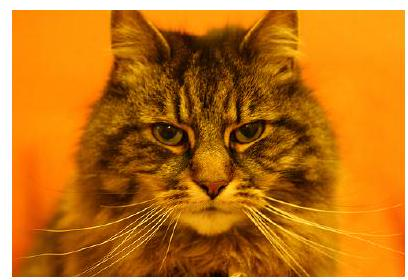
\includegraphics[max width=\textwidth]{2025_03_24_4f41283092a9d1f7a40eg-085} image, the system then asks whether it's the cat model or the dog model that better fits (is less surprised by) the image, and chooses that as its label.\\
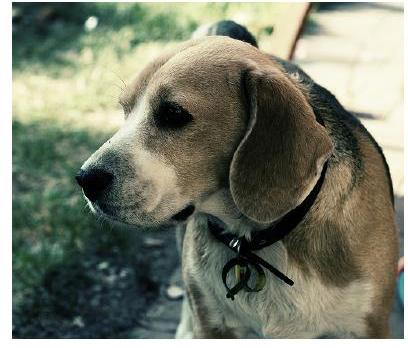
\includegraphics[max width=\textwidth, center]{2025_03_24_4f41283092a9d1f7a40eg-085(1)}

A discriminative model, by contrast, is only trying to learn to distinguish the classes (perhaps without learning much about them). So maybe all the dogs in the training data are wearing collars and the cats aren't. If that one feature neatly separates the classes, the model is satisfied. If you ask such a model what it knows about cats all it can say is that they don't wear collars.

More formally, recall that the naive Bayes assigns a class $c$ to a document $d$ not by directly computing $P(c \mid d)$ but by computing a likelihood and a prior

$$
\hat{c}=\underset{c \in C}{\operatorname{argmax}} \overbrace{P(d \mid c)}^{\text {likelihood }} \overbrace{P(c)}^{\text {prior }}
$$

generative model\\
discriminative model

A generative model like naive Bayes makes use of this likelihood term, which expresses how to generate the features of a document if we knew it was of class $c$.

By contrast a discriminative model in this text categorization scenario attempts to directly compute $P(c \mid d)$. Perhaps it will learn to assign a high weight to document features that directly improve its ability to discriminate between possible classes, even if it couldn't generate an example of one of the classes.

Components of a probabilistic machine learning classifier: Like naive Bayes, logistic regression is a probabilistic classifier that makes use of supervised machine learning. Machine learning classifiers require a training corpus of $m$ input/output pairs $\left(x^{(i)}, y^{(i)}\right)$. (We'll use superscripts in parentheses to refer to individual instances in the training set-for sentiment classification each instance might be an individual document to be classified.) A machine learning system for classification then has four components:

\begin{enumerate}
  \item A feature representation of the input. For each input observation $x^{(i)}$, this will be a vector of features $\left[x_{1}, x_{2}, \ldots, x_{n}\right]$. We will generally refer to feature $i$ for input $x^{(j)}$ as $x_{i}^{(j)}$, sometimes simplified as $x_{i}$, but we will also see the notation $f_{i}, f_{i}(x)$, or, for multiclass classification, $f_{i}(c, x)$.
  \item A classification function that computes $\hat{y}$, the estimated class, via $p(y \mid x)$. In the next section we will introduce the sigmoid and softmax tools for classification.
  \item An objective function that we want to optimize for learning, usually involving minimizing a loss function corresponding to error on training examples. We will introduce the cross-entropy loss function.
  \item An algorithm for optimizing the objective function. We introduce the stochastic gradient descent algorithm.\\
Logistic regression has two phases:\\
training: We train the system (specifically the weights $w$ and $b$, introduced below) using stochastic gradient descent and the cross-entropy loss.\\
test: Given a test example $x$ we compute $p(y \mid x)$ and return the higher probability label $y=1$ or $y=0$.
\end{enumerate}

\subsection*{5.1 The sigmoid function}
The goal of binary logistic regression is to train a classifier that can make a binary decision about the class of a new input observation. Here we introduce the sigmoid classifier that will help us make this decision.

Consider a single input observation $x$, which we will represent by a vector of features $\left[x_{1}, x_{2}, \ldots, x_{n}\right]$. (We'll show sample features in the next subsection.) The classifier output $y$ can be 1 (meaning the observation is a member of the class) or 0 (the observation is not a member of the class). We want to know the probability\\
$P(y=1 \mid x)$ that this observation is a member of the class. So perhaps the decision is "positive sentiment" versus "negative sentiment", the features represent counts of words in a document, $P(y=1 \mid x)$ is the probability that the document has positive sentiment, and $P(y=0 \mid x)$ is the probability that the document has negative sentiment.

Logistic regression solves this task by learning, from a training set, a vector of weights and a bias term. Each weight $w_{i}$ is a real number, and is associated with one of the input features $x_{i}$. The weight $w_{i}$ represents how important that input feature is to the classification decision, and can be positive (providing evidence that the instance being classified belongs in the positive class) or negative (providing evidence that the instance being classified belongs in the negative class). Thus we might expect in a sentiment task the word awesome to have a high positive weight, and\\
bias term intercept abysmal to have a very negative weight. The bias term,\\
another real number that's added to the weighted inputs.

To make a decision on a test instance-after we've learned the weights in trainingthe classifier first multiplies each $x_{i}$ by its weight $w_{i}$, sums up the weighted features, and adds the bias term $b$. The resulting single number $z$ expresses the weighted sum of the evidence for the class.


\begin{equation*}
z=\left(\sum_{i=1}^{n} w_{i} x_{i}\right)+b \tag{5.2}
\end{equation*}


In the rest of the book we'll represent such sums using the dot product notation from linear algebra. The dot product of two vectors $\mathbf{a}$ and $\mathbf{b}$, written as $\mathbf{a} \cdot \mathbf{b}$, is the sum of the products of the corresponding elements of each vector. (Notice that we represent vectors using the boldface notation $\mathbf{b}$ ). Thus the following is an equivalent formation to Eq. 5.2:


\begin{equation*}
z=\mathbf{w} \cdot \mathbf{x}+b \tag{5.3}
\end{equation*}


But note that nothing in Eq. 5.3 forces $z$ to be a legal probability, that is, to lie between 0 and 1 . In fact, since weights are real-valued, the output might even be negative; $z$ ranges from $-\infty$ to $\infty$.\\
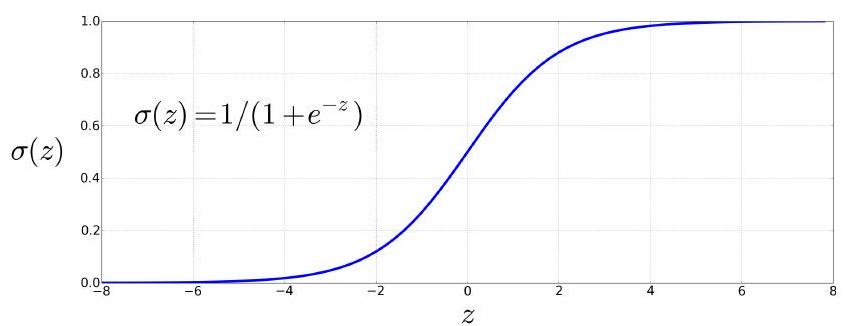
\includegraphics[max width=\textwidth, center]{2025_03_24_4f41283092a9d1f7a40eg-087}

Figure 5.1 The sigmoid function $\sigma(z)=\frac{1}{1+e^{-z}}$ takes a real value and maps it to the range $(0,1)$. It is nearly linear around 0 but outlier values get squashed toward 0 or 1 .

To create a probability, we'll pass $z$ through the sigmoid function, $\sigma(z)$. The sigmoid function (named because it looks like an $s$ ) is also called the logistic func-\\
shown graphically in Fig. 5.1:


\begin{equation*}
\sigma(z)=\frac{1}{1+e^{-z}}=\frac{1}{1+\exp (-z)} \tag{5.4}
\end{equation*}


(For the rest of the book, we'll use the notation $\exp (x)$ to mean $e^{x}$.) The sigmoid has a number of advantages; it takes a real-valued number and maps it into the range $(0,1)$, which is just what we want for a probability. Because it is nearly linear around 0 but flattens toward the ends, it tends to squash outlier values toward 0 or 1 . And it's differentiable, which as we'll see in Section 5.10 will be handy for learning.

We're almost there. If we apply the sigmoid to the sum of the weighted features, we get a number between 0 and 1 . To make it a probability, we just need to make sure that the two cases, $p(y=1)$ and $p(y=0)$, sum to 1 . We can do this as follows:


\begin{align*}
P(y=1) & =\sigma(\mathbf{w} \cdot \mathbf{x}+b) \\
& =\frac{1}{1+\exp (-(\mathbf{w} \cdot \mathbf{x}+b))} \\
P(y=0) & =1-\sigma(\mathbf{w} \cdot \mathbf{x}+b) \\
& =1-\frac{1}{1+\exp (-(\mathbf{w} \cdot \mathbf{x}+b))} \\
& =\frac{\exp (-(\mathbf{w} \cdot \mathbf{x}+b))}{1+\exp (-(\mathbf{w} \cdot \mathbf{x}+b))} \tag{5.5}
\end{align*}


The sigmoid function has the property


\begin{equation*}
1-\sigma(x)=\sigma(-x) \tag{5.6}
\end{equation*}


so we could also have expressed $P(y=0)$ as $\sigma(-(\mathbf{w} \cdot \mathbf{x}+b))$.\\
Finally, one terminological point. The input to the sigmoid function, the score logit $\quad z=\mathbf{w} \cdot \mathbf{x}+b$ from Eq. 5.3, is often called the logit. This is because the logit function is the inverse of the sigmoid. The logit function is the $\log$ of the odds ratio $\frac{p}{1-p}$ :


\begin{equation*}
\operatorname{logit}(p)=\sigma^{-1}(p)=\ln \frac{p}{1-p} \tag{5.7}
\end{equation*}


Using the term logit for $z$ is a way of reminding us that by using the sigmoid to turn $z$ (which ranges from $-\infty$ to $\infty$ ) into a probability, we are implicitly interpreting $z$ as not just any real-valued number, but as specifically a log odds.

\subsection*{5.2 Classification with Logistic Regression}
The sigmoid function from the prior section thus gives us a way to take an instance $x$ and compute the probability $P(y=1 \mid x)$.

How do we make a decision about which class to apply to a test instance $x$ ? For a given $x$, we say yes if the probability $P(y=1 \mid x)$ is more than .5 , and no otherwise.\\
decision boundary We call .5 the decision boundary:

$$
\operatorname{decision}(x)=\left\{\begin{array}{l}
1 \text { if } P(y=1 \mid x)>0.5 \\
0 \text { otherwise }
\end{array}\right.
$$

Let's have some examples of applying logistic regression as a classifier for language tasks.

\subsection*{5.2.1 Sentiment Classification}
Suppose we are doing binary sentiment classification on movie review text, and we would like to know whether to assign the sentiment class + or - to a review document $d o c$. We'll represent each input observation by the 6 features $x_{1} \ldots x_{6}$ of the input shown in the following table; Fig. 5.2 shows the features in a sample mini test document.

\begin{center}
\begin{tabular}{lll}
Var & Definition & Value in Fig. 5.2 \\
\hline
$x_{1}$ & count(positive lexicon words $\in \operatorname{doc})$ & 3 \\
$x_{2}$ & count(negative lexicon words $\in$ doc $)$ & 2 \\
$x_{3}$ & $\begin{cases}1 \text { if "no" } \in \text { doc } \\ 0 \text { otherwise }\end{cases}$ & 1 \\
$x_{4}$ & \begin{tabular}{l}
count $(1$ st and 2 nd pronouns $\in$ doc $)$ \\
\end{tabular} & 3 \\
$x_{5}$ & $\begin{cases}1 \text { if "!" } \in \text { doc } \\ 0 \text { otherwise }\end{cases}$ & 0 \\
$x_{6}$ & $\ln ($ word count of doc $)$ & $\ln (66)=4.19$ \\
\end{tabular}
\end{center}

\begin{center}
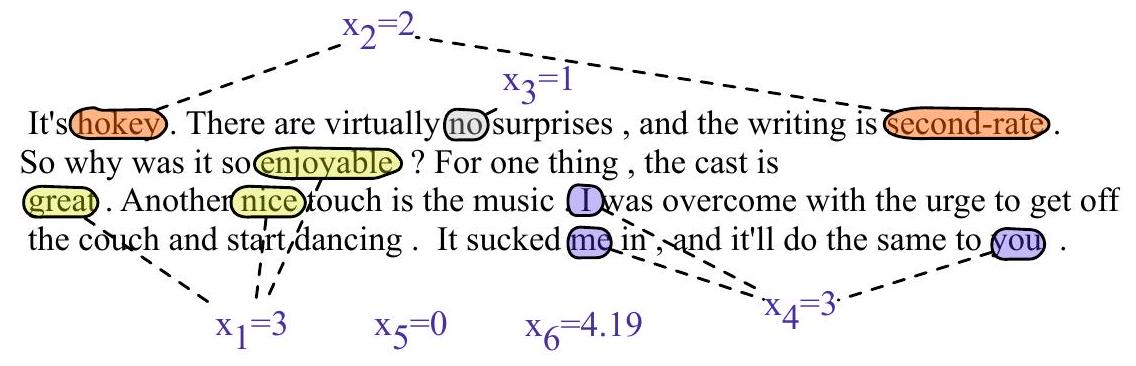
\includegraphics[max width=\textwidth]{2025_03_24_4f41283092a9d1f7a40eg-089}
\end{center}

Figure 5.2 A sample mini test document showing the extracted features in the vector $x$.

Let's assume for the moment that we've already learned a real-valued weight for each of these features, and that the 6 weights corresponding to the 6 features are $[2.5,-5.0,-1.2,0.5,2.0,0.7$ ], while $b=0.1$. (We'll discuss in the next section how the weights are learned.) The weight $w_{1}$, for example indicates how important a feature the number of positive lexicon words (great, nice, enjoyable, etc.) is to a positive sentiment decision, while $w_{2}$ tells us the importance of negative lexicon words. Note that $w_{1}=2.5$ is positive, while $w_{2}=-5.0$, meaning that negative words are negatively associated with a positive sentiment decision, and are about twice as important as positive words.

Given these 6 features and the input review $x, P(+\mid x)$ and $P(-\mid x)$ can be computed using Eq. 5.5:


\begin{align*}
p(+\mid x)=P(y=1 \mid x) & =\sigma(\mathbf{w} \cdot \mathbf{x}+b) \\
& =\sigma([2.5,-5.0,-1.2,0.5,2.0,0.7] \cdot[3,2,1,3,0,4.19]+0.1) \\
& =\sigma(.833) \\
& =0.70  \tag{5.8}\\
p(-\mid x)=P(y=0 \mid x) & =1-\sigma(\mathbf{w} \cdot \mathbf{x}+b) \\
& =0.30
\end{align*}


\subsection*{5.2.2 Other classification tasks and features}
Logistic regression is applied to all sorts of NLP tasks, and any property of the input

 can be a feature. Consider the task of period disambiguation: deciding if a period is the end of a sentence or part of a word, by classifying each period into one of two classes, EOS (end-of-sentence) and not-EOS. We might use features like $x_{1}$ below expressing that the current word is lower case, perhaps with a positive weight. Or a feature expressing that the current word is in our abbreviations dictionary ("Prof."), perhaps with a negative weight. A feature can also express a combination of properties. For example a period following an upper case word is likely to be an EOS, but if the word itself is $S t$. and the previous word is capitalized then the period is likely part of a shortening of the word street following a street name.

$$
\begin{aligned}
& x_{1}= \begin{cases}1 & \text { if "Case }\left(w_{i}\right)=\text { Lower" } \\
0 & \text { otherwise }\end{cases} \\
& x_{2}= \begin{cases}1 & \text { if " } w_{i} \in \text { AcronymDict" } \\
0 & \text { otherwise }\end{cases} \\
& x_{3}= \begin{cases}1 & \text { if " } w_{i}=\operatorname{St} . \& \operatorname{Case}\left(w_{i-1}\right)=\text { Upper" } \\
0 & \text { otherwise }\end{cases}
\end{aligned}
$$

Designing versus learning features: In classic models, features are designed by hand by examining the training set with an eye to linguistic intuitions and literature, supplemented by insights from error analysis on the training set of an early version of a system. We can also consider (feature interactions), complex features that are combinations of more primitive features. We saw such a feature for period disambiguation above, where a period on the word St. was less likely to be the end of the sentence if the previous word was capitalized. Features can be created automatically via feature templates, abstract specifications of features. For example a bigram template for period disambiguation might create a feature for every pair of words that occurs before a period in the training set. Thus the feature space is sparse, since we only have to create a feature if that $n$-gram exists in that position in the training set. The feature is generally created as a hash from the string descriptions. A user description of a feature as, "bigram(American breakfast)" is hashed into a unique integer $i$ that becomes the feature number $f_{i}$.

It should be clear from the prior paragraph that designing features by hand requires extensive human effort. For this reason, recent NLP systems avoid handdesigned features and instead focus on representation learning: ways to learn features automatically in an unsupervised way from the input. We'll introduce methods for representation learning in Chapter 6 and Chapter 7.\\
Scaling input features: When different input features have extremely different ranges of values, it's common to rescale them so they have comparable ranges. We standardize input values by centering them to result in a zero mean and a standard deviation of one (this transformation is sometimes called the z-score). That is, if $\mu_{i}$ is the mean of the values of feature $x_{i}$ across the $m$ observations in the input dataset, and $\sigma_{i}$ is the standard deviation of the values of features $x_{i}$ across the input dataset, we can replace each feature $x_{i}$ by a new feature $x_{i}^{\prime}$ computed as follows:


\begin{gather*}
\mu_{i}=\frac{1}{m} \sum_{j=1}^{m} x_{i}^{(j)} \quad \sigma_{i}=\sqrt{\frac{1}{m} \sum_{j=1}^{m}\left(x_{i}^{(j)}-\mu_{i}\right)^{2}} \\
x_{i}^{\prime}=\frac{x_{i}-\mu_{i}}{\sigma_{i}} \tag{5.9}
\end{gather*}


normalize\\
Alternatively, we can normalize the input features values to lie between 0 and 1:


\begin{equation*}
x_{i}^{\prime}=\frac{x_{i}-\min \left(x_{i}\right)}{\max \left(x_{i}\right)-\min \left(x_{i}\right)} \tag{5.10}
\end{equation*}


Having input data with comparable range is useful when comparing values across features. Data scaling is especially important in large neural networks, since it helps speed up gradient descent.

\subsection*{5.2.3 Processing many examples at once}
We've shown the equations for logistic regression for a single example. But in practice we'll of course want to process an entire test set with many examples. Let's suppose we have a test set consisting of $m$ test examples each of which we'd like to classify. We'll continue to use the notation from page 78, in which a superscript value in parentheses refers to the example index in some set of data (either for training or for test). So in this case each test example $x^{(i)}$ has a feature vector $\mathbf{x}^{(i)}$, $1 \leq i \leq m$. (As usual, we'll represent vectors and matrices in bold.)

One way to compute each output value $\hat{y}^{(i)}$ is just to have a for-loop, and compute each test example one at a time:


\begin{align*}
& \text { foreach } x^{(i)} \text { in input }\left[x^{(1)}, x^{(2)}, \ldots, x^{(m)}\right] \\
& y^{(i)}=\sigma\left(\mathbf{w} \cdot \mathbf{x}^{(\mathbf{i})}+b\right) \tag{5.11}
\end{align*}


For the first 3 test examples, then, we would be separately computing the predicted $\hat{y}^{(i)}$ as follows:

$$
\begin{aligned}
& P\left(y^{(1)}=1 \mid x^{(1)}\right)=\sigma\left(\mathbf{w} \cdot \mathbf{x}^{(1)}+b\right) \\
& P\left(y^{(2)}=1 \mid x^{(2)}\right)=\sigma\left(\mathbf{w} \cdot \mathbf{x}^{(2)}+b\right) \\
& P\left(y^{(3)}=1 \mid x^{(3)}\right)=\sigma\left(\mathbf{w} \cdot \mathbf{x}^{(3)}+b\right)
\end{aligned}
$$

But it turns out that we can slightly modify our original equation Eq. 5.5 to do this much more efficiently. We'll use matrix arithmetic to assign a class to all the examples with one matrix operation!

First, we'll pack all the input feature vectors for each input $x$ into a single input matrix $\mathbf{X}$, where each row $i$ is a row vector consisting of the feature vector for input example $x^{(i)}$ (i.e., the vector $\mathbf{x}^{(i)}$ ). Assuming each example has $f$ features and weights, $\mathbf{X}$ will therefore be a matrix of shape $[m \times f]$, as follows:

\[
\mathbf{X}=\left[\begin{array}{cccc}
x_{1}^{(1)} & x_{2}^{(1)} & \ldots & x_{f}^{(1)}  \tag{5.12}\\
x_{1}^{(2)} & x_{2}^{(2)} & \ldots & x_{f}^{(2)} \\
x_{1}^{(3)} & x_{2}^{(3)} & \ldots & x_{f}^{(3)} \\
\ldots & & &
\end{array}\right]
\]

Now if we introduce $\mathbf{b}$ as a vector of length $m$ which consists of the scalar bias term $b$ repeated $m$ times, $\mathbf{b}=[b, b, \ldots, b]$, and $\hat{\mathbf{y}}=\left[\hat{y}^{(1)}, \hat{y}^{(2)} \ldots, \hat{y}^{(m)}\right]$ as the vector of outputs (one scalar $\hat{y}^{(i)}$ for each input $x^{(i)}$ and its feature vector $\mathbf{x}^{(i)}$ ), and represent the weight vector $\mathbf{w}$ as a column vector, we can compute all the outputs with a single matrix multiplication and one addition:


\begin{equation*}
\mathbf{y}=\mathbf{X} \mathbf{w}+\mathbf{b} \tag{5.13}
\end{equation*}


You should convince yourself that Eq. 5.13 computes the same thing as our for-loop in Eq. 5.11. For example $\hat{y}^{(1)}$, the first entry of the output vector $\mathbf{y}$, will correctly be:


\begin{equation*}
\hat{y}^{(1)}=\left[x_{1}^{(1)}, x_{2}^{(1)}, \ldots, x_{f}^{(1)}\right] \cdot\left[w_{1}, w_{2}, \ldots, w_{f}\right]+b \tag{5.14}
\end{equation*}


Note that we had to reorder $\mathbf{X}$ and $\mathbf{w}$ from the order they appeared in in Eq. 5.5 to make the multiplications come out properly. Here is Eq. 5.13 again with the shapes shown:


\begin{align*}
\mathbf{y}= & \mathbf{X} \quad \mathbf{w}+\mathbf{b} \\
(m \times 1) & (m \times f)(f \times 1)(m \times 1) \tag{5.15}
\end{align*}


Modern compilers and compute hardware can compute this matrix operation very efficiently, making the computation much faster, which becomes important when training or testing on very large datasets.

Note by the way that we could have kept $\mathbf{X}$ and $\mathbf{w}$ in the original order $(\mathbf{y}=$ $\mathbf{X} \mathbf{w}+\mathbf{b}$ ) if we had chosen to define $\mathbf{X}$ differently as a matrix of column vectors, one vector for each input example, instead of row vectors, and then it would have shape $[f \times m]$. But we conventionally represent inputs as rows.

\subsection*{5.2.4 Choosing a classifier}
Logistic regression has a number of advantages over naive Bayes. Naive Bayes has overly strong conditional independence assumptions. Consider two features which are strongly correlated; in fact, imagine that we just add the same feature $f_{1}$ twice. Naive Bayes will treat both copies of $f_{1}$ as if they were separate, multiplying them both in, overestimating the evidence. By contrast, logistic regression is much more robust to correlated features; if two features $f_{1}$ and $f_{2}$ are perfectly correlated, regression will simply assign part of the weight to $w_{1}$ and part to $w_{2}$. Thus when there are many correlated features, logistic regression will assign a more accurate probability than naive Bayes. So logistic regression generally works better on larger documents or datasets and is a common default.

Despite the less accurate probabilities, naive Bayes still often makes the correct classification decision. Furthermore, naive Bayes can work extremely well (sometimes even better than logistic regression) on very small datasets ( Ng and Jordan, 2002) or short documents (Wang and Manning, 2012). Furthermore, naive Bayes is easy to implement and very fast to train (there's no optimization step). So it's still a reasonable approach to use in some situations.

\subsection*{5.3 Multinomial logistic regression}
Sometimes we need more than two classes. Perhaps we might want to do 3-way sentiment classification (positive, negative, or neutral). Or we could be assigning some of the labels we will introduce in Chapter 17, like the part of speech of a word (choosing from 10, 30, or even 50 different parts of speech), or the named entity type of a phrase (choosing from tags like person, location, organization).

In such cases we use multinomial logistic regression, also called softmax regression (in older NLP literature you will sometimes see the name maxent classifier). In multinomial logistic regression we want to label each observation with a class $k$ from a set of $K$ classes, under the stipulation that only one of these classes is\\
the correct one (sometimes called hard classification; an observation can not be in multiple classes). Let's use the following representation: the output $\mathbf{y}$ for each input $\mathbf{x}$ will be a vector of length $K$. If class $c$ is the correct class, we'll set $y_{c}=1$, and set all the other elements of $\boldsymbol{y}$ to be 0 , i.e., $y_{c}=1$ and $y_{j}=0 \quad \forall j \neq c$. A vector like this $\mathbf{y}$, with one value $=1$ and the rest 0 , is called a one-hot vector. The job of the classifier is to produce an estimate vector $\hat{\mathbf{y}}$. For each class $k$, the value $\hat{y}_{k}$ will be the classifier's estimate of the probability $p\left(y_{k}=1 \mid \mathbf{x}\right)$.

\subsection*{5.3.1 Softmax}
The multinomial logistic classifier uses a generalization of the sigmoid, called the softmax function, to compute $p\left(y_{k}=1 \mid \mathbf{x}\right)$. The softmax function takes a vector $\mathbf{z}=\left[z_{1}, z_{2}, \ldots, z_{K}\right]$ of $K$ arbitrary values and maps them to a probability distribution, with each value in the range $[0,1]$, and all the values summing to 1 . Like the sigmoid, it is an exponential function.

For a vector $\mathbf{z}$ of dimensionality $K$, the softmax is defined as:


\begin{equation*}
\operatorname{softmax}\left(z_{i}\right)=\frac{\exp \left(z_{i}\right)}{\sum_{j=1}^{K} \exp \left(z_{j}\right)} 1 \leq i \leq K \tag{5.16}
\end{equation*}


The softmax of an input vector $\mathbf{z}=\left[z_{1}, z_{2}, \ldots, z_{K}\right]$ is thus a vector itself:


\begin{equation*}
\operatorname{softmax}(\mathbf{z})=\left[\frac{\exp \left(z_{1}\right)}{\sum_{i=1}^{K} \exp \left(z_{i}\right)}, \frac{\exp \left(z_{2}\right)}{\sum_{i=1}^{K} \exp \left(z_{i}\right)}, \ldots, \frac{\exp \left(z_{K}\right)}{\sum_{i=1}^{K} \exp \left(z_{i}\right)}\right] \tag{5.17}
\end{equation*}


The denominator $\sum_{i=1}^{K} \exp \left(\mathbf{z}_{i}\right)$ is used to normalize all the values into probabilities. Thus for example given a vector:

$$
\mathbf{z}=[0.6,1.1,-1.5,1.2,3.2,-1.1]
$$

the resulting (rounded) $\operatorname{softmax}(\mathbf{z})$ is

$$
[0.05,0.09,0.01,0.1,0.74,0.01]
$$

Like the sigmoid, the softmax has the property of squashing values toward 0 or 1 . Thus if one of the inputs is larger than the others, it will tend to push its probability toward 1, and suppress the probabilities of the smaller inputs.

Finally, note that, just as for the sigmoid, we refer to $\mathbf{z}$, the vector of scores that is the input to the softmax, as logits (see Eq. 5.7).

\subsection*{5.3.2 Applying softmax in logistic regression}
When we apply softmax for logistic regression, the input will (just as for the sigmoid) be the dot product between a weight vector $\mathbf{w}$ and an input vector $\mathbf{x}$ (plus a bias). But now we'll need separate weight vectors $\mathbf{w}_{k}$ and bias $b_{k}$ for each of the $K$ classes. The probability of each of our output classes $\hat{y}_{k}$ can thus be computed as:


\begin{equation*}
p\left(y_{k}=1 \mid \mathbf{x}\right)=\frac{\exp \left(\mathbf{w}_{k} \cdot \mathbf{x}+b_{k}\right)}{\sum_{j=1}^{K} \exp \left(\mathbf{w}_{j} \cdot \mathbf{x}+b_{j}\right)} \tag{5.18}
\end{equation*}


The form of Eq. 5.18 makes it seem that we would compute each output separately. Instead, it's more common to set up the equation for more efficient computation by modern vector processing hardware. We'll do this by representing the set of $K$ weight vectors as a weight matrix $W$ and a bias vector $\mathbf{b}$. Each row $k$ of $\mathbf{W}$ corresponds to the vector of weights $w_{k}$. $\mathbf{W}$ thus has shape $[K \times f]$, for $K$ the number of output classes and $f$ the number of input features. The bias vector $\mathbf{b}$ has one value for each of the $K$ output classes. If we represent the weights in this way, we can compute $\hat{\mathbf{y}}$, the vector of output probabilities for each of the $K$ classes, by a single elegant equation:


\begin{equation*}
\hat{\mathbf{y}}=\operatorname{softmax}(\mathbf{W} \mathbf{x}+\mathbf{b}) \tag{5.19}
\end{equation*}


If you work out the matrix arithmetic, you can see that the estimated score of the first output class $\hat{y}_{1}$ (before we take the softmax) will correctly turn out to be $\mathbf{w}_{1} \cdot \mathbf{x}+b_{1}$.

One helpful interpretation of the weight matrix $\mathbf{W}$ is to see each row $\mathbf{w}_{k}$ as a prototype of class $k$. The weight vector $\mathbf{w}_{k}$ that is learned represents the class as a kind of template. Since two vectors that are more similar to each other have a higher dot product with each other, the dot product acts as a similarity function. Logistic regression is thus learning an exemplar representation for each class, such that incoming vectors are assigned the class $k$ they are most similar to from the $K$ classes.

Fig. 5.3 shows the difference between binary and multinomial logistic regression by illustrating the weight vector versus weight matrix in the computation of the output class probabilities.

\subsection*{5.3.3 Features in Multinomial Logistic Regression}
Features in multinomial logistic regression act like features in binary logistic regression, with the difference mentioned above that we'll need separate weight vectors and biases for each of the $K$ classes. Recall our binary exclamation point feature $x_{5}$ from page 81:

$$
x_{5}=\left\{\begin{array}{l}
1 \text { if } "!" \in \text { doc } \\
0 \text { otherwise }
\end{array}\right.
$$

In binary classification a positive weight $w_{5}$ on a feature influences the classifier toward $y=1$ (positive sentiment) and a negative weight influences it toward $y=0$ (negative sentiment) with the absolute value indicating how important the feature is. For multinomial logistic regression, by contrast, with separate weights for each class, a feature can be evidence for or against each individual class.

In 3-way multiclass sentiment classification, for example, we must assign each document one of the 3 classes,+- , or 0 (neutral). Now a feature related to exclamation marks might have a negative weight for 0 documents, and a positive weight for + or - documents:

\begin{center}
\begin{tabular}{lllll}
Feature & Definition & $w_{5,+}$ & $w_{5,-}$ & $w_{5,0}$ \\
\hline
$f_{5}(x)$ & $\left\{\begin{array}{llll}1 & \text { if } "!" \in \operatorname{doc} \\ 0 & \text { otherwise }\end{array}\right.$ & 3.5 & 3.1 & -5.3 \\
\hline
\end{tabular}
\end{center}

Because these feature weights are dependent both on the input text and the output class, we sometimes make this dependence explicit and represent the features themselves as $f(x, y)$ : a function of both the input and the class. Using such a notation\\
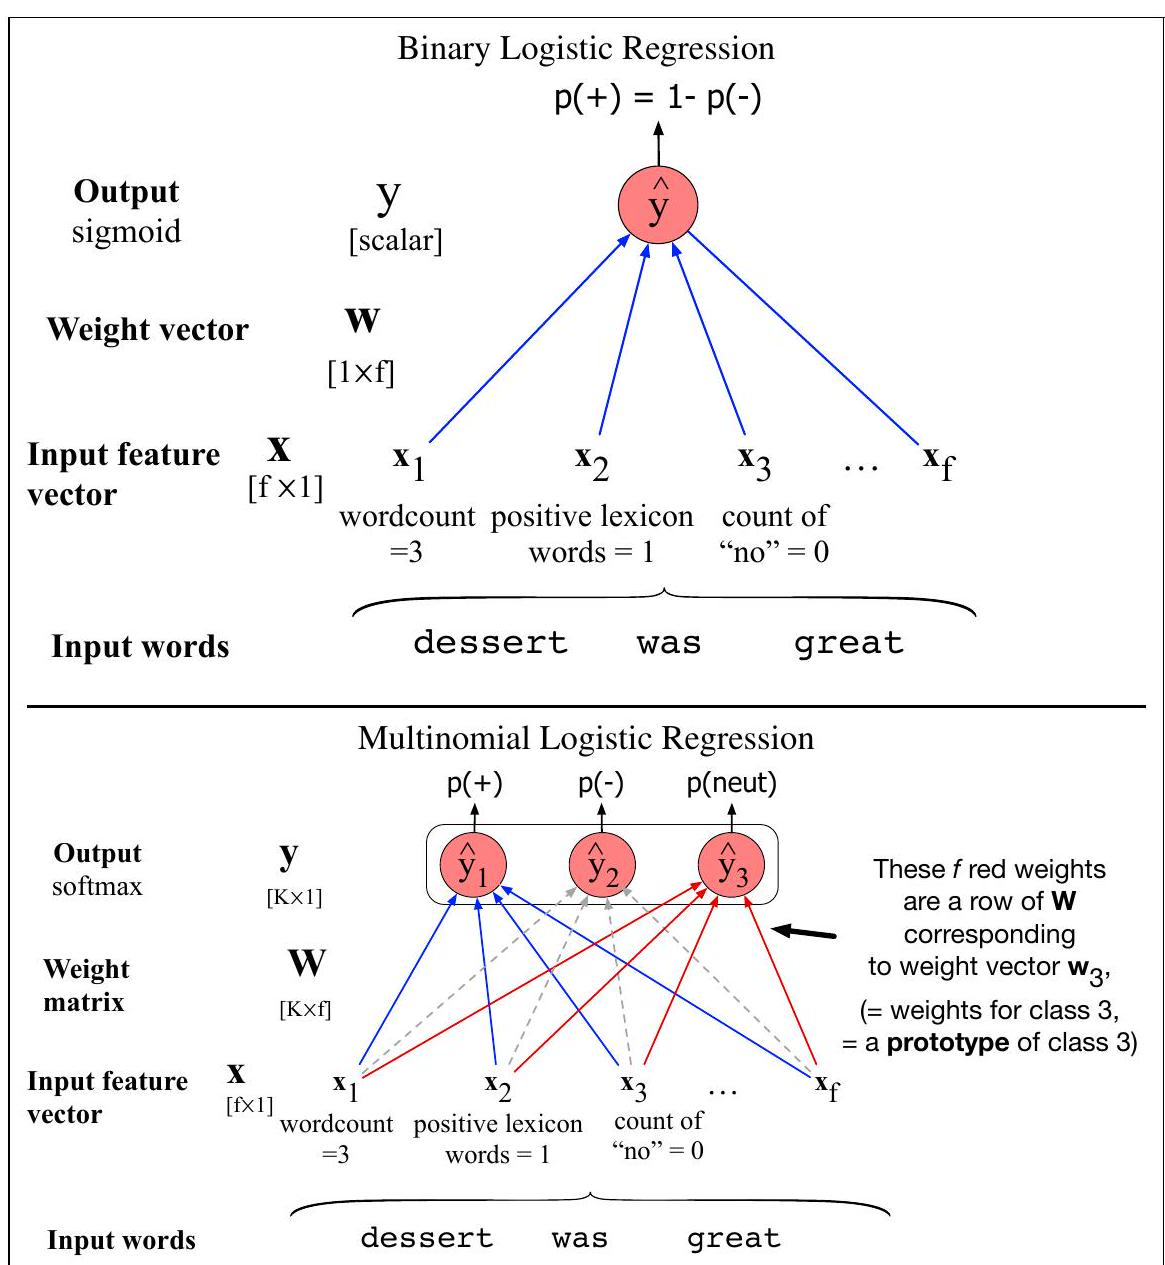
\includegraphics[max width=\textwidth, center]{2025_03_24_4f41283092a9d1f7a40eg-095}

Figure 5.3 Binary versus multinomial logistic regression. Binary logistic regression uses a single weight vector $\mathbf{w}$, and has a scalar output $\hat{y}$. In multinomial logistic regression we have $K$ separate weight vectors corresponding to the $K$ classes, all packed into a single weight matrix $\mathbf{W}$, and a vector output $\hat{\mathbf{y}}$. We omit the biases from both figures for clarity.\\
$f_{5}(x)$ above could be represented as three features $f_{5}(x,+), f_{5}(x,-)$, and $f_{5}(x, 0)$, each of which has a single weight. We'll use this kind of notation in our description of the CRF in Chapter 17.

\subsection*{5.4 Learning in Logistic Regression}
How are the parameters of the model, the weights $\mathbf{w}$ and bias $b$, learned? Logistic regression is an instance of supervised classification in which we know the correct label $y$ (either 0 or 1) for each observation $x$. What the system produces via Eq. 5.5 is $\hat{y}$, the system's estimate of the true $y$. We want to learn parameters (meaning $\mathbf{w}$ and $b$ ) that make $\hat{y}$ for each training observation as close as possible to the true $y$.

This requires two components that we foreshadowed in the introduction to the chapter. The first is a metric for how close the current label $(\hat{y})$ is to the true gold\\
label $y$. Rather than measure similarity, we usually talk about the opposite of this: the distance between the system output and the gold output, and we call this distance the loss function or the cost function. In the next section we'll introduce the loss function that is commonly used for logistic regression and also for neural networks, the cross-entropy loss.

The second thing we need is an optimization algorithm for iteratively updating the weights so as to minimize this loss function. The standard algorithm for this is gradient descent; we'll introduce the stochastic gradient descent algorithm in the following section.

We'll describe these algorithms for the simpler case of binary logistic regression in the next two sections, and then turn to multinomial logistic regression in Section 5.8.

\subsection*{5.5 The cross-entropy loss function}
We need a loss function that expresses, for an observation $x$, how close the classifier output $(\hat{y}=\sigma(\mathbf{w} \cdot \mathbf{x}+b))$ is to the correct output ( $y$, which is 0 or 1 ). We'll call this:


\begin{equation*}
L(\hat{y}, y)=\text { How much } \hat{y} \text { differs from the true } y \tag{5.20}
\end{equation*}


We do this via a loss function that prefers the correct class labels of the training examples to be more likely. This is called conditional maximum likelihood estimation: we choose the parameters $w, b$ that maximize the log probability of the true $y$ labels in the training data given the observations $x$. The resulting loss function is the negative log likelihood loss, generally called the cross-entropy loss.

Let's derive this loss function, applied to a single observation $x$. We'd like to learn weights that maximize the probability of the correct label $p(y \mid x)$. Since there are only two discrete outcomes ( 1 or 0 ), this is a Bernoulli distribution, and we can express the probability $p(y \mid x)$ that our classifier produces for one observation as the following (keeping in mind that if $y=1$, Eq. 5.21 simplifies to $\hat{y}$; if $y=0$, Eq. 5.21 simplifies to $1-\hat{y}$ ):


\begin{equation*}
p(y \mid x)=\hat{y}^{y}(1-\hat{y})^{1-y} \tag{5.21}
\end{equation*}


Now we take the log of both sides. This will turn out to be handy mathematically, and doesn't hurt us; whatever values maximize a probability will also maximize the $\log$ of the probability:


\begin{align*}
\log p(y \mid x) & =\log \left[\hat{y}^{y}(1-\hat{y})^{1-y}\right] \\
& =y \log \hat{y}+(1-y) \log (1-\hat{y}) \tag{5.22}
\end{align*}


Eq. 5.22 describes a log likelihood that should be maximized. In order to turn this into a loss function (something that we need to minimize), we'll just flip the sign on Eq. 5.22. The result is the cross-entropy loss $L_{\mathrm{CE}}$ :


\begin{equation*}
L_{\mathrm{CE}}(\hat{y}, y)=-\log p(y \mid x)=-[y \log \hat{y}+(1-y) \log (1-\hat{y})] \tag{5.23}
\end{equation*}


Finally, we can plug in the definition of $\hat{y}=\sigma(\mathbf{w} \cdot \mathbf{x}+b)$ :


\begin{equation*}
L_{\mathrm{CE}}(\hat{y}, y)=-[y \log \sigma(\mathbf{w} \cdot \mathbf{x}+b)+(1-y) \log (1-\sigma(\mathbf{w} \cdot \mathbf{x}+b))] \tag{5.24}
\end{equation*}


Let's see if this loss function does the right thing for our example from Fig. 5.2. We want the loss to be smaller if the model's estimate is close to correct, and bigger if the model is confused. So first let's suppose the correct gold label for the sentiment example in Fig. 5.2 is positive, i.e., $y=1$. In this case our model is doing well, since from Eq. 5.8 it indeed gave the example a higher probability of being positive (.70) than negative (.30). If we plug $\sigma(\mathbf{w} \cdot \mathbf{x}+b)=.70$ and $y=1$ into Eq. 5.24 , the right side of the equation drops out, leading to the following loss (we'll use log to mean natural $\log$ when the base is not specified):

$$
\begin{array}{rlrl}
L_{\mathrm{CE}}(\hat{y}, y) & = & & -[y \log \sigma(\mathbf{w} \cdot \mathbf{x}+b)+(1-y) \log (1-\sigma(\mathbf{w} \cdot \mathbf{x}+b))] \\
& = & -[\log \sigma(\mathbf{w} \cdot \mathbf{x}+b)] \\
& = & & -\log (.70) \\
& = & & .36
\end{array}
$$

By contrast, let's pretend instead that the example in Fig. 5.2 was actually negative, i.e., $y=0$ (perhaps the reviewer went on to say "But bottom line, the movie is terrible! I beg you not to see it!"). In this case our model is confused and we'd want the loss to be higher. Now if we plug $y=0$ and $1-\sigma(\mathbf{w} \cdot \mathbf{x}+b)=.30$ from Eq. 5.8 into Eq. 5.24, the left side of the equation drops out:

$$
\begin{array}{rlrl}
L_{\mathrm{CE}}(\hat{y}, y) & = & -[y \log \sigma(\mathbf{w} \cdot \mathbf{x}+b)+(1-y) \log (1-\sigma(\mathbf{w} \cdot \mathbf{x}+b))] \\
& = & & -[\log (1-\sigma(\mathbf{w} \cdot \mathbf{x}+b))] \\
& = & -\log (.30) \\
& = & 1.2
\end{array}
$$

Sure enough, the loss for the first classifier (.36) is less than the loss for the second classifier (1.2).

Why does minimizing this negative log probability do what we want? A perfect classifier would assign probability 1 to the correct outcome $(y=1$ or $y=0)$ and probability 0 to the incorrect outcome. That means if $y$ equals 1 , the higher $\hat{y}$ is (the closer it is to 1 ), the better the classifier; the lower $\hat{y}$ is (the closer it is to 0 ), the worse the classifier. If $y$ equals 0 , instead, the higher $1-\hat{y}$ is (closer to 1 ), the better the classifier. The negative $\log$ of $\hat{y}$ (if the true $y$ equals 1 ) or $1-\hat{y}$ (if the true $y$ equals 0 ) is a convenient loss metric since it goes from 0 (negative log of 1 , no loss) to infinity (negative log of 0 , infinite loss). This loss function also ensures that as the probability of the correct answer is maximized, the probability of the incorrect answer is minimized; since the two sum to one, any increase in the probability of the correct answer is coming at the expense of the incorrect answer. It's called the crossentropy loss, because Eq. 5.22 is also the formula for the cross-entropy between the true probability distribution $y$ and our estimated distribution $\hat{y}$.

Now we know what we want to minimize; in the next section, we'll see how to find the minimum.

\subsection*{5.6 Gradient Descent}
Our goal with gradient descent is to find the optimal weights: minimize the loss function we've defined for the model. In Eq. 5.25 below, we'll explicitly represent the fact that the cross-entropy loss function $L_{\mathrm{CE}}$ is parameterized by the weights. In\\
machine learning in general we refer to the parameters being learned as $\theta$; in the case of logistic regression $\theta=\{\mathbf{w}, b\}$. So the goal is to find the set of weights which minimizes the loss function, averaged over all examples:


\begin{equation*}
\hat{\theta}=\underset{\theta}{\operatorname{argmin}} \frac{1}{m} \sum_{i=1}^{m} L_{\mathrm{CE}}\left(f\left(x^{(i)} ; \theta\right), y^{(i)}\right) \tag{5.25}
\end{equation*}


How shall we find the minimum of this (or any) loss function? Gradient descent is a method that finds a minimum of a function by figuring out in which direction (in the space of the parameters $\theta$ ) the function's slope is rising the most steeply, and moving in the opposite direction. The intuition is that if you are hiking in a canyon and trying to descend most quickly down to the river at the bottom, you might look around yourself in all directions, find the direction where the ground is sloping the steepest, and walk downhill in that direction.

For logistic regression, this loss function is conveniently convex. A convex function has at most one minimum; there are no local minima to get stuck in, so gradient descent starting from any point is guaranteed to find the minimum. (By contrast, the loss for multi-layer neural networks is non-convex, and gradient descent may get stuck in local minima for neural network training and never find the global optimum.)

Although the algorithm (and the concept of gradient) are designed for direction vectors, let's first consider a visualization of the case where the parameter of our system is just a single scalar $w$, shown in Fig. 5.4.

Given a random initialization of $w$ at some value $w^{1}$, and assuming the loss function $L$ happened to have the shape in Fig. 5.4, we need the algorithm to tell us whether at the next iteration we should move left (making $w^{2}$ smaller than $w^{1}$ ) or right (making $w^{2}$ bigger than $w^{1}$ ) to reach the minimum.\\
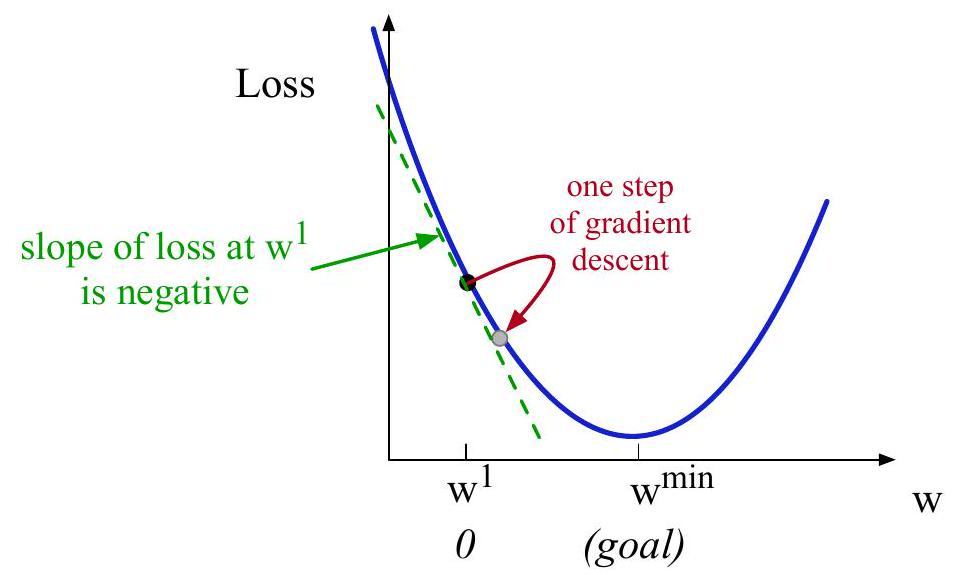
\includegraphics[max width=\textwidth, center]{2025_03_24_4f41283092a9d1f7a40eg-098}

Figure 5.4 The first step in iteratively finding the minimum of this loss function, by moving $w$ in the reverse direction from the slope of the function. Since the slope is negative, we need to move $w$ in a positive direction, to the right. Here superscripts are used for learning steps, so $w^{1}$ means the initial value of $w$ (which is 0 ), $w^{2}$ the value at the second step, and so on.

The gradient descent algorithm answers this question by finding the gradient of the loss function at the current point and moving in the opposite direction. The gradient of a function of many variables is a vector pointing in the direction of the greatest increase in a function. The gradient is a multi-variable generalization of the\\
slope, so for a function of one variable like the one in Fig. 5.4, we can informally think of the gradient as the slope. The dotted line in Fig. 5.4 shows the slope of this hypothetical loss function at point $w=w^{1}$. You can see that the slope of this dotted line is negative. Thus to find the minimum, gradient descent tells us to go in the opposite direction: moving $w$ in a positive direction.

The magnitude of the amount to move in gradient descent is the value of the slope $\frac{d}{d w} L(f(x ; w), y)$ weighted by a learning rate $\eta$. A higher (faster) learning rate means that we should move $w$ more on each step. The change we make in our parameter is the learning rate times the gradient (or the slope, in our single-variable example):


\begin{equation*}
w^{t+1}=w^{t}-\eta \frac{d}{d w} L(f(x ; w), y) \tag{5.26}
\end{equation*}


Now let's extend the intuition from a function of one scalar variable $w$ to many variables, because we don't just want to move left or right, we want to know where in the N -dimensional space (of the $N$ parameters that make up $\theta$ ) we should move. The gradient is just such a vector; it expresses the directional components of the sharpest slope along each of those $N$ dimensions. If we're just imagining two weight dimensions (say for one weight $w$ and one bias $b$ ), the gradient might be a vector with two orthogonal components, each of which tells us how much the ground slopes in the $w$ dimension and in the $b$ dimension. Fig. 5.5 shows a visualization of the value of a 2-dimensional gradient vector taken at the red point.

In an actual logistic regression, the parameter vector $\mathbf{w}$ is much longer than 1 or 2 , since the input feature vector $\mathbf{x}$ can be quite long, and we need a weight $w_{i}$ for each $x_{i}$. For each dimension/variable $w_{i}$ in $\mathbf{w}$ (plus the bias $b$ ), the gradient will have a component that tells us the slope with respect to that variable. In each dimension $w_{i}$, we express the slope as a partial derivative $\frac{\partial}{\partial w_{i}}$ of the loss function. Essentially we're asking: "How much would a small change in that variable $w_{i}$ influence the total loss function $L$ ?"

Formally, then, the gradient of a multi-variable function $f$ is a vector in which each component expresses the partial derivative of $f$ with respect to one of the variables. We'll use the inverted Greek delta symbol $\nabla$ to refer to the gradient, and\\
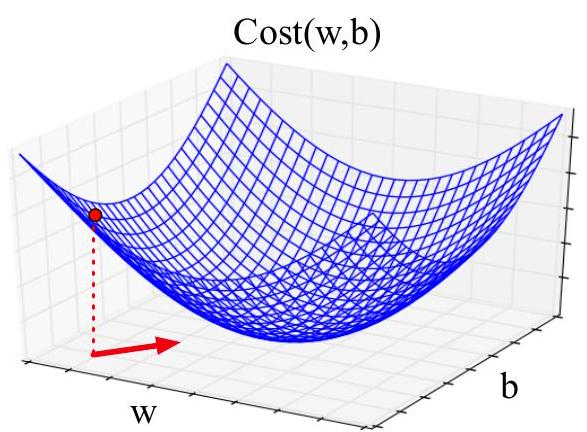
\includegraphics[max width=\textwidth, center]{2025_03_24_4f41283092a9d1f7a40eg-099}

Figure 5.5 Visualization of the gradient vector at the red point in two dimensions $w$ and $b$, showing a red arrow in the x - y plane pointing in the direction we will go to look for the minimum: the opposite direction of the gradient (recall that the gradient points in the direction of increase not decrease).\\
represent $\hat{y}$ as $f(x ; \theta)$ to make the dependence on $\theta$ more obvious:

\[
\nabla L(f(x ; \theta), y)=\left[\begin{array}{c}
\frac{\partial}{\partial w_{1}} L(f(x ; \theta), y)  \tag{5.27}\\
\frac{\partial}{\partial w_{2}} L(f(x ; \theta), y) \\
\vdots \\
\frac{\partial}{\partial w_{n}} L(f(x ; \theta), y) \\
\frac{\partial}{\partial b} L(f(x ; \theta), y)
\end{array}\right]
\]

The final equation for updating $\theta$ based on the gradient is thus


\begin{equation*}
\theta^{t+1}=\theta^{t}-\eta \nabla L(f(x ; \theta), y) \tag{5.28}
\end{equation*}


\subsection*{5.6.1 The Gradient for Logistic Regression}
In order to update $\theta$, we need a definition for the gradient $\nabla L(f(x ; \theta), y)$. Recall that for logistic regression, the cross-entropy loss function is:


\begin{equation*}
L_{\mathrm{CE}}(\hat{y}, y)=-[y \log \sigma(\mathbf{w} \cdot \mathbf{x}+b)+(1-y) \log (1-\sigma(\mathbf{w} \cdot \mathbf{x}+b))] \tag{5.29}
\end{equation*}


It turns out that the derivative of this function for one observation vector $x$ is Eq. 5.30 (the interested reader can see Section 5.10 for the derivation of this equation):


\begin{align*}
\frac{\partial L_{\mathrm{CE}}(\hat{y}, y)}{\partial w_{j}} & =[\sigma(\mathbf{w} \cdot \mathbf{x}+b)-y] x_{j} \\
& =(\hat{y}-y) x_{j} \tag{5.30}
\end{align*}


You'll also sometimes see this equation in the equivalent form:


\begin{equation*}
\frac{\partial L_{\mathrm{CE}}(\hat{y}, y)}{\partial w_{j}}=-(y-\hat{y}) x_{j} \tag{5.31}
\end{equation*}


Note in these equations that the gradient with respect to a single weight $w_{j}$ represents a very intuitive value: the difference between the true $y$ and our estimated $\hat{y}=\sigma(\mathbf{w} \cdot \mathbf{x}+b)$ for that observation, multiplied by the corresponding input value $x_{j}$.

\subsection*{5.6.2 The Stochastic Gradient Descent Algorithm}
Stochastic gradient descent is an online algorithm that minimizes the loss function by computing its gradient after each training example, and nudging $\theta$ in the right direction (the opposite direction of the gradient). (An "online algorithm" is one that processes its input example by example, rather than waiting until it sees the entire input.) Stochastic gradient descent is called stochastic because it chooses a single random example at a time; in Section 5.6.4 we'll discuss other versions of gradient descent that batch many examples at once. Fig. 5.6 shows the algorithm.

The learning rate $\eta$ is a hyperparameter that must be adjusted. If it's too high, the learner will take steps that are too large, overshooting the minimum of the loss function. If it's too low, the learner will take steps that are too small, and take too long to get to the minimum. It is common to start with a higher learning rate and then slowly decrease it, so that it is a function of the iteration $k$ of training; the notation $\eta_{k}$ can be used to mean the value of the learning rate at iteration $k$.

\begin{verbatim}
function Stochastic Gradient $\operatorname{Descent}(L(), f(), x, y)$ returns $\theta$
    \# where: L is the loss function
    \# f is a function parameterized by $\theta$
    \# x is the set of training inputs $x^{(1)}, x^{(2)}, \ldots, x^{(m)}$
    \# $\quad \mathrm{y}$ is the set of training outputs (labels) $y^{(1)}, y^{(2)}, \ldots, y^{(m)}$
$\theta \leftarrow 0 \quad$ \# (or small random values)
repeat til done \# see caption
    For each training tuple $\left(x^{(i)}, y^{(i)}\right)$ (in random order)
        1. Optional (for reporting): \# How are we doing on this tuple?
                Compute $\hat{y}^{(i)}=f\left(x^{(i)} ; \theta\right) \quad$ \# What is our estimated output $\hat{y}$ ?
            Compute the loss $L\left(\hat{y}^{(i)}, y^{(i)}\right)$ \# How far off is $\hat{y}^{(i)}$ from the true output $y^{(i)}$ ?
        2. $g \leftarrow \nabla_{\theta} L\left(f\left(x^{(i)} ; \theta\right), y^{(i)}\right) \quad$ \# How should we move $\theta$ to maximize loss?
        3. $\theta \leftarrow \theta-\eta g \quad$ \# Go the other way instead
return $\theta$
\end{verbatim}

Figure 5.6 The stochastic gradient descent algorithm. Step 1 (computing the loss) is used mainly to report how well we are doing on the current tuple; we don't need to compute the loss in order to compute the gradient. The algorithm can terminate when it converges (when the gradient norm $<\epsilon$ ), or when progress halts (for example when the loss starts going up on a held-out set). Weights are initialized to 0 for logistic regression, but to small random values for neural networks, as we'll see in Chapter 7.

We'll discuss hyperparameters in more detail in Chapter 7, but in short, they are a special kind of parameter for any machine learning model. Unlike regular parameters of a model (weights like $w$ and $b$ ), which are learned by the algorithm from the training set, hyperparameters are special parameters chosen by the algorithm designer that affect how the algorithm works.

\subsection*{5.6.3 Working through an example}
Let's walk through a single step of the gradient descent algorithm. We'll use a simplified version of the example in Fig. 5.2 as it sees a single observation $x$, whose correct value is $y=1$ (this is a positive review), and with a feature vector $\mathbf{x}=\left[x_{1}, x_{2}\right]$ consisting of these two features:

$$
\begin{array}{ll}
x_{1}=3 & \text { (count of positive lexicon words) } \\
x_{2}=2 & \text { (count of negative lexicon words) }
\end{array}
$$

Let's assume the initial weights and bias in $\theta^{0}$ are all set to 0 , and the initial learning rate $\eta$ is 0.1 :

$$
\begin{aligned}
w_{1}=w_{2}=b & =0 \\
\eta & =0.1
\end{aligned}
$$

The single update step requires that we compute the gradient, multiplied by the learning rate

$$
\theta^{t+1}=\theta^{t}-\eta \nabla_{\theta} L\left(f\left(x^{(i)} ; \theta\right), y^{(i)}\right)
$$

In our mini example there are three parameters, so the gradient vector has 3 dimensions, for $w_{1}, w_{2}$, and $b$. We can compute the first gradient as follows:

$$
\nabla_{w, b} L=\left[\begin{array}{l}
\frac{\partial L_{\mathrm{CE}}(\hat{y}, y)}{\partial w,} \\
\frac{\partial L_{\mathrm{CE}}(\hat{y}, y)}{\partial w} \\
\frac{\partial L_{\mathrm{CE}}(\hat{y}, y)}{\partial b}
\end{array}\right]=\left[\begin{array}{l}
(\sigma(\mathbf{w} \cdot \mathbf{x}+b)-y) x_{1} \\
(\sigma(\mathbf{w} \cdot \mathbf{x}+b)-y) x_{2} \\
\sigma(\mathbf{w} \cdot \mathbf{x}+b)-y
\end{array}\right]=\left[\begin{array}{l}
(\sigma(0)-1) x_{1} \\
(\sigma(0)-1) x_{2} \\
\sigma(0)-1
\end{array}\right]=\left[\begin{array}{l}
-0.5 x_{1} \\
-0.5 x_{2} \\
-0.5
\end{array}\right]=\left[\begin{array}{l}
-1.5 \\
-1.0 \\
-0.5
\end{array}\right]
$$

Now that we have a gradient, we compute the new parameter vector $\theta^{1}$ by moving $\theta^{0}$ in the opposite direction from the gradient:

$$
\theta^{1}=\left[\begin{array}{l}
w_{1} \\
w_{2} \\
b
\end{array}\right]-\eta\left[\begin{array}{l}
-1.5 \\
-1.0 \\
-0.5
\end{array}\right]=\left[\begin{array}{l}
.15 \\
.1 \\
.05
\end{array}\right]
$$

So after one step of gradient descent, the weights have shifted to be: $w_{1}=.15$, $w_{2}=.1$, and $b=.05$.

Note that this observation $x$ happened to be a positive example. We would expect that after seeing more negative examples with high counts of negative words, that the weight $\mathbf{w}_{2}$ would shift to have a negative value.

\subsection*{5.6.4 Mini-batch training}
Stochastic gradient descent is called stochastic because it chooses a single random example at a time, moving the weights so as to improve performance on that single example. That can result in very choppy movements, so it's common to compute the gradient over batches of training instances rather than a single instance.

For example in batch training we compute the gradient over the entire dataset. By seeing so many examples, batch training offers a superb estimate of which direction to move the weights, at the cost of spending a lot of time processing every single example in the training set to compute this perfect direction.

A compromise is mini-batch training: we train on a group of $m$ examples (perhaps 512 , or 1024 ) that is less than the whole dataset. (If $m$ is the size of the dataset, then we are doing batch gradient descent; if $m=1$, we are back to doing stochastic gradient descent.) Mini-batch training also has the advantage of computational efficiency. The mini-batches can easily be vectorized, choosing the size of the minibatch based on the computational resources. This allows us to process all the examples in one mini-batch in parallel and then accumulate the loss, something that's not possible with individual or batch training.

We just need to define mini-batch versions of the cross-entropy loss function we defined in Section 5.5 and the gradient in Section 5.6.1. Let's extend the crossentropy loss for one example from Eq. 5.23 to mini-batches of size $m$. We'll continue to use the notation that $x^{(i)}$ and $y^{(i)}$ mean the $i$ th training features and training label, respectively. We make the assumption that the training examples are independent:


\begin{align*}
\log p(\text { training labels }) & =\log \prod_{i=1}^{m} p\left(y^{(i)} \mid x^{(i)}\right) \\
& =\sum_{i=1}^{m} \log p\left(y^{(i)} \mid x^{(i)}\right) \\
& =-\sum_{i=1}^{m} L_{\mathrm{CE}}\left(\hat{y}^{(i)}, y^{(i)}\right) \tag{5.32}
\end{align*}


Now the cost function for the mini-batch of $m$ examples is the average loss for each example:


\begin{align*}
\operatorname{Cost}(\hat{y}, y) & =\frac{1}{m} \sum_{i=1}^{m} L_{\mathrm{CE}}\left(\hat{y}^{(i)}, y^{(i)}\right) \\
& =-\frac{1}{m} \sum_{i=1}^{m} y^{(i)} \log \sigma\left(\mathbf{w} \cdot \mathbf{x}^{(i)}+b\right)+\left(1-y^{(i)}\right) \log \left(1-\sigma\left(\mathbf{w} \cdot \mathbf{x}^{(i)}+b\right)\right) \tag{5.33}
\end{align*}


The mini-batch gradient is the average of the individual gradients from Eq. 5.30:


\begin{equation*}
\frac{\partial \operatorname{Cost}(\hat{y}, y)}{\partial w_{j}}=\frac{1}{m} \sum_{i=1}^{m}\left[\sigma\left(\mathbf{w} \cdot \mathbf{x}^{(i)}+b\right)-y^{(i)}\right] x_{j}^{(i)} \tag{5.34}
\end{equation*}


Instead of using the sum notation, we can more efficiently compute the gradient in its matrix form, following the vectorization we saw on page 83 , where we have a matrix $\mathbf{X}$ of size $[m \times f]$ representing the $m$ inputs in the batch, and a vector $\mathbf{y}$ of size $[m \times 1]$ representing the correct outputs:


\begin{align*}
\frac{\partial \operatorname{Cost}(\hat{y}, y)}{\partial \mathbf{w}} & =\frac{1}{m}(\hat{\mathbf{y}}-\mathbf{y})^{\top} \mathbf{X} \\
& =\frac{1}{m}(\sigma(\mathbf{X} \mathbf{w}+\mathbf{b})-\mathbf{y})^{\top} \mathbf{X} \tag{5.35}
\end{align*}


\subsection*{5.7 Regularization}
Numquam ponenda est pluralitas sine necessitate 'Plurality should never be proposed unless needed'

William of Occam\\
overfitting\\
generalize regularization

There is a problem with learning weights that make the model perfectly match the training data. If a feature is perfectly predictive of the outcome because it happens to only occur in one class, it will be assigned a very high weight. The weights for features will attempt to perfectly fit details of the training set, in fact too perfectly, modeling noisy factors that just accidentally correlate with the class. This problem is called overfitting. A good model should be able to generalize well from the training data to the unseen test set, but a model that overfits will have poor generalization.

To avoid overfitting, a new regularization term $R(\theta)$ is added to the loss function in Eq. 5.25 , resulting in the following loss for a batch of $m$ examples (slightly rewritten from Eq. 5.25 to be maximizing log probability rather than minimizing loss, and removing the $\frac{1}{m}$ term which doesn't affect the argmax):


\begin{equation*}
\hat{\theta}=\underset{\theta}{\operatorname{argmax}} \sum_{i=1}^{m} \log P\left(y^{(i)} \mid x^{(i)}\right)-\alpha R(\theta) \tag{5.36}
\end{equation*}


The new regularization term $R(\theta)$ is used to penalize large weights. Thus a setting of the weights that matches the training data perfectly - but uses many weights with

L2\\
regularization\\
high values to do so-will be penalized more than a setting that matches the data a little less well, but does so using smaller weights. There are two common ways to compute this regularization term $R(\theta)$. $\mathbf{L} 2$ regularization is a quadratic function of the weight values, named because it uses the (square of the) L 2 norm of the weight values. The L2 norm, $\|\theta\|_{2}$, is the same as the Euclidean distance of the vector $\theta$ from the origin. If $\theta$ consists of $n$ weights, then:


\begin{equation*}
R(\theta)=\|\theta\|_{2}^{2}=\sum_{j=1}^{n} \theta_{j}^{2} \tag{5.37}
\end{equation*}


The L2 regularized loss function becomes:


\begin{equation*}
\hat{\theta}=\underset{\theta}{\operatorname{argmax}}\left[\sum_{i=1}^{m} \log P\left(y^{(i)} \mid x^{(i)}\right)\right]-\alpha \sum_{j=1}^{n} \theta_{j}^{2} \tag{5.38}
\end{equation*}


L1 regularization is a linear function of the weight values, named after the L1 norm $\|W\|_{1}$, the sum of the absolute values of the weights, or Manhattan distance (the Manhattan distance is the distance you'd have to walk between two points in a city with a street grid like New York):


\begin{equation*}
R(\theta)=\|\theta\|_{1}=\sum_{i=1}^{n}\left|\theta_{i}\right| \tag{5.39}
\end{equation*}


The L1 regularized loss function becomes:


\begin{equation*}
\hat{\theta}=\underset{\theta}{\operatorname{argmax}}\left[\sum_{i=1}^{m} \log P\left(y^{(i)} \mid x^{(i)}\right)\right]-\alpha \sum_{j=1}^{n}\left|\theta_{j}\right| \tag{5.40}
\end{equation*}


These kinds of regularization come from statistics, where L 1 regularization is called\\
lasso\\
ridge\\
lasso regression (Tibshirani, 1996) and L 2 regularization is called ridge regression, and both are commonly used in language processing. L2 regularization is easier to optimize because of its simple derivative (the derivative of $\theta^{2}$ is just $2 \theta$ ), while L1 regularization is more complex (the derivative of $|\theta|$ is non-continuous at zero). But while L2 prefers weight vectors with many small weights, L1 prefers sparse solutions with some larger weights but many more weights set to zero. Thus L1 regularization leads to much sparser weight vectors, that is, far fewer features.

Both L1 and L2 regularization have Bayesian interpretations as constraints on the prior of how weights should look. L1 regularization can be viewed as a Laplace prior on the weights. L2 regularization corresponds to assuming that weights are distributed according to a Gaussian distribution with mean $\mu=0$. In a Gaussian or normal distribution, the further away a value is from the mean, the lower its probability (scaled by the variance $\sigma$ ). By using a Gaussian prior on the weights, we are saying that weights prefer to have the value 0 . A Gaussian for a weight $\theta_{j}$ is


\begin{equation*}
\frac{1}{\sqrt{2 \pi \sigma_{j}^{2}}} \exp \left(-\frac{\left(\theta_{j}-\mu_{j}\right)^{2}}{2 \sigma_{j}^{2}}\right) \tag{5.41}
\end{equation*}


If we multiply each weight by a Gaussian prior on the weight, we are thus maximizing the following constraint:


\begin{equation*}
\hat{\theta}=\underset{\theta}{\operatorname{argmax}} \prod_{i=1}^{m} P\left(y^{(i)} \mid x^{(i)}\right) \times \prod_{j=1}^{n} \frac{1}{\sqrt{2 \pi \sigma_{j}^{2}}} \exp \left(-\frac{\left(\theta_{j}-\mu_{j}\right)^{2}}{2 \sigma_{j}^{2}}\right) \tag{5.42}
\end{equation*}


which in $\log$ space, with $\mu=0$, and assuming $2 \sigma^{2}=1$, corresponds to


\begin{equation*}
\hat{\theta}=\underset{\theta}{\operatorname{argmax}} \sum_{i=1}^{m} \log P\left(y^{(i)} \mid x^{(i)}\right)-\alpha \sum_{j=1}^{n} \theta_{j}^{2} \tag{5.43}
\end{equation*}


which is in the same form as Eq. 5.38 .

\subsection*{5.8 Learning in Multinomial Logistic Regression}
The loss function for multinomial logistic regression generalizes the loss function for binary logistic regression from 2 to $K$ classes. Recall that that the cross-entropy loss for binary logistic regression (repeated from Eq. 5.23) is:


\begin{equation*}
L_{\mathrm{CE}}(\hat{y}, y)=-\log p(y \mid x)=-[y \log \hat{y}+(1-y) \log (1-\hat{y})] \tag{5.44}
\end{equation*}


The loss function for multinomial logistic regression generalizes the two terms in Eq. 5.44 (one that is non-zero when $y=1$ and one that is non-zero when $y=0$ ) to $K$ terms. As we mentioned above, for multinomial regression we'll represent both $\mathbf{y}$ and $\hat{\mathbf{y}}$ as vectors. The true label $\mathbf{y}$ is a vector with $K$ elements, each corresponding to a class, with $y_{c}=1$ if the correct class is $c$, with all other elements of $\mathbf{y}$ being 0 . And our classifier will produce an estimate vector with $K$ elements $\hat{\mathbf{y}}$, each element $\hat{y}_{k}$ of which represents the estimated probability $p\left(y_{k}=1 \mid \mathbf{x}\right)$.

The loss function for a single example $\mathbf{x}$, generalizing from binary logistic regression, is the sum of the logs of the $K$ output classes, each weighted by the indicator function $\mathbf{y}_{k}$ (Eq. 5.45). This turns out to be just the negative log probability of the correct class $c$ (Eq. 5.46):


\begin{align*}
L_{\mathrm{CE}}(\hat{\mathbf{y}}, \mathbf{y}) & =-\sum_{k=1}^{K} y_{k} \log \hat{y}_{k}  \tag{5.45}\\
& =-\log \hat{y}_{c}, \quad(\text { where } c \text { is the correct class) }  \tag{5.46}\\
& =-\log \hat{p}\left(y_{c}=1 \mid \mathbf{x}\right) \quad(\text { where } c \text { is the correct class) } \\
& =-\log \frac{\exp \left(\mathbf{w}_{\mathbf{c}} \cdot \mathbf{x}+b_{c}\right)}{\sum_{j=1}^{K} \exp \left(\mathbf{w}_{\mathbf{j}} \cdot \mathbf{x}+b_{j}\right)} \quad(c \text { is the correct class) } \tag{5.47}
\end{align*}


How did we get from Eq. 5.45 to Eq. 5.46? Because only one class (let's call it $c$ ) is the correct one, the vector $\mathbf{y}$ takes the value 1 only for this value of $k$, i.e., has $y_{c}=1$ and $y_{j}=0 \forall j \neq c$. That means the terms in the sum in Eq. 5.45 will all be 0 except for the term corresponding to the true class $c$. Hence the cross-entropy loss is simply the $\log$ of the output probability corresponding to the correct class, and we therefore also call Eq. 5.46 the negative log likelihood loss.

Of course for gradient descent we don't need the loss, we need its gradient. The gradient for a single example turns out to be very similar to the gradient for binary logistic regression, $(\hat{y}-y) x$, that we saw in Eq. 5.30. Let's consider one piece of the gradient, the derivative for a single weight. For each class $k$, the weight of the $i$ th element of input $\mathbf{x}$ is $w_{k, i}$. What is the partial derivative of the loss with respect to $w_{k, i}$ ? This derivative turns out to be just the difference between the true value for the class $k$ (which is either 1 or 0 ) and the probability the classifier outputs for class $k$,\\
weighted by the value of the input $x_{i}$ corresponding to the $i$ th element of the weight vector for class $k$ :


\begin{align*}
\frac{\partial L_{\mathrm{CE}}}{\partial w_{k, i}} & =-\left(y_{k}-\hat{y}_{k}\right) x_{i} \\
& =-\left(y_{k}-p\left(y_{k}=1 \mid x\right)\right) x_{i} \\
& =-\left(y_{k}-\frac{\exp \left(\mathbf{w}_{\mathbf{k}} \cdot \mathbf{x}+b_{k}\right)}{\sum_{j=1}^{K} \exp \left(\mathbf{w}_{\mathbf{j}} \cdot \mathbf{x}+b_{j}\right)}\right) x_{i} \tag{5.48}
\end{align*}


We'll return to this case of the gradient for softmax regression when we introduce neural networks in Chapter 7, and at that time we'll also discuss the derivation of this gradient in equations Eq. 7.33-Eq. 7.41.

\subsection*{5.9 Interpreting models}
Often we want to know more than just the correct classification of an observation. We want to know why the classifier made the decision it did. That is, we want our\\
interpretable decision to be interpretable. Interpretability can be hard to define strictly, but the core idea is that as humans we should know why our algorithms reach the conclusions they do. Because the features to logistic regression are often human-designed, one way to understand a classifier's decision is to understand the role each feature plays in the decision. Logistic regression can be combined with statistical tests (the likelihood ratio test, or the Wald test); investigating whether a particular feature is significant by one of these tests, or inspecting its magnitude (how large is the weight $w$ associated with the feature?) can help us interpret why the classifier made the decision it makes. This is enormously important for building transparent models.

Furthermore, in addition to its use as a classifier, logistic regression in NLP and many other fields is widely used as an analytic tool for testing hypotheses about the effect of various explanatory variables (features). In text classification, perhaps we want to know if logically negative words (no, not, never) are more likely to be associated with negative sentiment, or if negative reviews of movies are more likely to discuss the cinematography. However, in doing so it's necessary to control for potential confounds: other factors that might influence sentiment (the movie genre, the year it was made, perhaps the length of the review in words). Or we might be studying the relationship between NLP-extracted linguistic features and non-linguistic outcomes (hospital readmissions, political outcomes, or product sales), but need to control for confounds (the age of the patient, the county of voting, the brand of the product). In such cases, logistic regression allows us to test whether some feature is associated with some outcome above and beyond the effect of other features.

\subsection*{5.10 Advanced: Deriving the Gradient Equation}
In this section we give the derivation of the gradient of the cross-entropy loss function $L_{\mathrm{CE}}$ for logistic regression. Let's start with some quick calculus refreshers. First, the derivative of $\ln (x)$ :


\begin{equation*}
\frac{d}{d x} \ln (x)=\frac{1}{x} \tag{5.49}
\end{equation*}


Second, the (very elegant) derivative of the sigmoid:


\begin{equation*}
\frac{d \sigma(z)}{d z}=\sigma(z)(1-\sigma(z)) \tag{5.50}
\end{equation*}


chain rule\\
Finally, the chain rule of derivatives. Suppose we are computing the derivative of a composite function $f(x)=u(v(x))$. The derivative of $f(x)$ is the derivative of $u(x)$ with respect to $v(x)$ times the derivative of $v(x)$ with respect to $x$ :


\begin{equation*}
\frac{d f}{d x}=\frac{d u}{d v} \cdot \frac{d v}{d x} \tag{5.51}
\end{equation*}


First, we want to know the derivative of the loss function with respect to a single weight $w_{j}$ (we'll need to compute it for each weight, and for the bias):


\begin{align*}
\frac{\partial L_{\mathrm{CE}}}{\partial w_{j}} & =\frac{\partial}{\partial w_{j}}-[y \log \sigma(\mathbf{w} \cdot \mathbf{x}+b)+(1-y) \log (1-\sigma(\mathbf{w} \cdot \mathbf{x}+b))] \\
& =-\left[\frac{\partial}{\partial w_{j}} y \log \sigma(\mathbf{w} \cdot \mathbf{x}+b)+\frac{\partial}{\partial w_{j}}(1-y) \log [1-\sigma(\mathbf{w} \cdot \mathbf{x}+b)]\right] \tag{5.52}
\end{align*}


Next, using the chain rule, and relying on the derivative of log:


\begin{equation*}
\frac{\partial L_{\mathrm{CE}}}{\partial w_{j}}=-\frac{y}{\sigma(\mathbf{w} \cdot \mathbf{x}+b)} \frac{\partial}{\partial w_{j}} \sigma(\mathbf{w} \cdot \mathbf{x}+b)-\frac{1-y}{1-\sigma(\mathbf{w} \cdot \mathbf{x}+b)} \frac{\partial}{\partial w_{j}} 1-\sigma(\mathbf{w} \cdot \mathbf{x}+b) \tag{5.53}
\end{equation*}


Rearranging terms:


\begin{equation*}
\frac{\partial L_{\mathrm{CE}}}{\partial w_{j}}=-\left[\frac{y}{\sigma(\mathbf{w} \cdot \mathbf{x}+b)}-\frac{1-y}{1-\sigma(\mathbf{w} \cdot \mathbf{x}+b)}\right] \frac{\partial}{\partial w_{j}} \sigma(\mathbf{w} \cdot \mathbf{x}+b) \tag{5.54}
\end{equation*}


And now plugging in the derivative of the sigmoid, and using the chain rule one more time, we end up with Eq. 5.55:


\begin{align*}
\frac{\partial L_{\mathrm{CE}}}{\partial w_{j}} & =-\left[\frac{y-\sigma(\mathbf{w} \cdot \mathbf{x}+b)}{\sigma(\mathbf{w} \cdot \mathbf{x}+b)[1-\sigma(\mathbf{w} \cdot \mathbf{x}+b)]}\right] \sigma(\mathbf{w} \cdot \mathbf{x}+b)[1-\sigma(\mathbf{w} \cdot \mathbf{x}+b)] \frac{\partial(\mathbf{w} \cdot \mathbf{x}+b)}{\partial w_{j}} \\
& =-\left[\frac{y-\sigma(\mathbf{w} \cdot \mathbf{x}+b)}{\sigma(\mathbf{w} \cdot \mathbf{x}+b)[1-\sigma(\mathbf{w} \cdot \mathbf{x}+b)]}\right] \sigma(\mathbf{w} \cdot \mathbf{x}+b)[1-\sigma(\mathbf{w} \cdot \mathbf{x}+b)] x_{j} \\
& =-[y-\sigma(\mathbf{w} \cdot \mathbf{x}+b)] x_{j} \\
& =[\sigma(\mathbf{w} \cdot \mathbf{x}+b)-y] x_{j} \tag{5.55}
\end{align*}


\subsection*{5.11 Summary}
This chapter introduced the logistic regression model of classification.

\begin{itemize}
  \item Logistic regression is a supervised machine learning classifier that extracts real-valued features from the input, multiplies each by a weight, sums them, and passes the sum through a sigmoid function to generate a probability. A threshold is used to make a decision.
  \item Logistic regression can be used with two classes (e.g., positive and negative sentiment) or with multiple classes (multinomial logistic regression, for example for n-ary text classification, part-of-speech labeling, etc.).
  \item Multinomial logistic regression uses the softmax function to compute probabilities.
  \item The weights (vector $w$ and bias $b$ ) are learned from a labeled training set via a loss function, such as the cross-entropy loss, that must be minimized.
  \item Minimizing this loss function is a convex optimization problem, and iterative algorithms like gradient descent are used to find the optimal weights.
  \item Regularization is used to avoid overfitting.
  \item Logistic regression is also one of the most useful analytic tools, because of its ability to transparently study the importance of individual features.
\end{itemize}

\section*{Bibliographical and Historical Notes}
Logistic regression was developed in the field of statistics, where it was used for the analysis of binary data by the 1960 s, and was particularly common in medicine (Cox, 1969). Starting in the late 1970s it became widely used in linguistics as one of the formal foundations of the study of linguistic variation (Sankoff and Labov, 1979).

Nonetheless, logistic regression didn't become common in natural language processing until the 1990s, when it seems to have appeared simultaneously from two directions. The first source was the neighboring fields of information retrieval and speech processing, both of which had made use of regression, and both of which lent many other statistical techniques to NLP. Indeed a very early use of logistic regression for document routing was one of the first NLP applications to use (LSI) embeddings as word representations (Schütze et al., 1995).

At the same time in the early 1990s logistic regression was developed and applied to NLP at IBM Research under the name maximum entropy modeling or maxent (Berger et al., 1996), seemingly independent of the statistical literature. Under that name it was applied to language modeling (Rosenfeld, 1996), part-of-speech tagging (Ratnaparkhi, 1996), parsing (Ratnaparkhi, 1997), coreference resolution (Kehler, 1997b), and text classification (Nigam et al., 1999).

More on classification can be found in machine learning textbooks (Hastie et al. 2001, Witten and Frank 2005, Bishop 2006, Murphy 2012).

\section*{Exercises}
\section*{Vector Semantics and Embeddings }
庄子(Zhuangzi),Chapter 26\\
The asphalt that Los Angeles is famous for occurs mainly on its freeways.But in the middle of the city is another patch of asphalt,the La Brea tar pits,and this asphalt preserves millions of fossil bones from the last of the Ice Ages of the Pleis- tocene Epoch.One of these fossils is the Smilodon,or saber-toothed tiger,instantly recognizable by its long canines.Five million years ago or so,a completely different saber-tooth tiger called Thylacosmilus lived in Argentina and other parts of South Amer- ica.Thylacosmilus was a marsupial whereas Smilodon was a placental mammal,but Thy- lacosmilus had the same long upper canines and,like Smilodon,had a protective bone flange on the lower jaw.The similarity of these two mammals is one of many examples\\

\includegraphics[max width=\textwidth]{2025_03_24_4f41283092a9d1f7a40eg-109} of parallel or convergent evolution,in which particular contexts or environments lead to the evolution of very similar structures in different species(Gould,1980).

The role of context is also important in the similarity of a less biological kind of organism:the word.Words that occur in similar contexts tend to have similar meanings.This link between similarity in how words are distributed and similarity\\
distributional hypothesis\\
vector in what they mean is called the distributional hypothesis.The hypothesis was first formulated in the 1950s by linguists like Joos(1950),Harris(1954),and Firth (1957),who noticed that words which are synonyms(like oculist and eye-doctor) tended to occur in the same environment(e.g.,near words like eye or examined) with the amount of meaning difference between two words"corresponding roughly to the amount of difference in their environments"(Harris,1954,p.157).

In this chapter we introduce vector semantics,which instantiates this linguistic hypothesis by learning representations of the meaning of words,called embeddings, directly from their distributions in texts.These representations are used in every nat- ural language processing application that makes use of meaning,and the static em- beddings we introduce here underlie the more powerful dynamic or contextualized embeddings like BERT that we will see in Chapter 11.

These word representations are also the first example in this book of repre- sentation learning,automatically learning useful representations of the input text. Finding such self-supervised ways to learn representations of the input,instead of creating representations by hand via feature engineering,is an important focus of NLP research(Bengio et al.,2013).

\subsection*{6.1 Lexical Semantics}
Let's begin by introducing some basic principles of word meaning. How should we represent the meaning of a word? In the n-gram models of Chapter 3, and in classical NLP applications, our only representation of a word is as a string of letters, or an index in a vocabulary list. This representation is not that different from a tradition in philosophy, perhaps you've seen it in introductory logic classes, in which the meaning of words is represented by just spelling the word with small capital letters; representing the meaning of "dog" as DOG, and "cat" as CAT, or by using an apostrophe (DOG').

Representing the meaning of a word by capitalizing it is a pretty unsatisfactory model. You might have seen a version of a joke due originally to semanticist Barbara Partee (Carlson, 1977):

Q: What's the meaning of life?\\
A: LIFE'\\
Surely we can do better than this! After all, we'll want a model of word meaning to do all sorts of things for us. It should tell us that some words have similar meanings (cat is similar to $d o g$ ), others are antonyms (cold is the opposite of hot), some have positive connotations (happy) while others have negative connotations (sad). It should represent the fact that the meanings of buy, sell, and pay offer differing perspectives on the same underlying purchasing event. (If I buy something from you, you've probably sold it to me, and I likely paid you.) More generally, a model of word meaning should allow us to draw inferences to address meaning-related tasks like question-answering or dialogue.

In this section we summarize some of these desiderata, drawing on results in the linguistic study of word meaning, which is called lexical semantics; we'll return to and expand on this list in Appendix G and Chapter 21.

Lemmas and Senses Let's start by looking at how one word (we'll choose mouse) might be defined in a dictionary (simplified from the online dictionary WordNet):

\begin{verbatim}
mouse (N)
\end{verbatim}

\begin{enumerate}
  \item any of numerous small rodents...
  \item a hand-operated device that controls a cursor...
\end{enumerate}

Here the form mouse is the lemma, also called the citation form. The form mouse would also be the lemma for the word mice; dictionaries don't have separate definitions for inflected forms like mice. Similarly sing is the lemma for sing, sang, sung. In many languages the infinitive form is used as the lemma for the verb, so Spanish dormir "to sleep" is the lemma for duermes "you sleep". The specific forms sung or carpets or sing or duermes are called wordforms.

As the example above shows, each lemma can have multiple meanings; the lemma mouse can refer to the rodent or the cursor control device. We call each of these aspects of the meaning of mouse a word sense. The fact that lemmas can be polysemous (have multiple senses) can make interpretation difficult (is someone who types "mouse info" into a search engine looking for a pet or a tool?). Chapter 11 and Appendix G will discuss the problem of polysemy, and introduce word sense disambiguation, the task of determining which sense of a word is being used in a particular context.\\
Synonymy One important component of word meaning is the relationship between word senses. For example when one word has a sense whose meaning is\\
identical to a sense of another word, or nearly identical, we say the two senses of those two words are synonyms. Synonyms include such pairs as

\section*{couch/sofa vomit/throw up filbert/hazelnut car/automobile}
A more formal definition of synonymy (between words rather than senses) is that two words are synonymous if they are substitutable for one another in any sentence without changing the truth conditions of the sentence, the situations in which the sentence would be true.

While substitutions between some pairs of words like car / automobile or water / $\mathrm{H}_{2} \mathrm{O}$ are truth preserving, the words are still not identical in meaning. Indeed, probably no two words are absolutely identical in meaning. One of the fundamental tenets of semantics, called the principle of contrast (Girard 1718, Bréal 1897, Clark 1987), states that a difference in linguistic form is always associated with some difference in meaning. For example, the word $\mathrm{H}_{2} \mathrm{O}$ is used in scientific contexts and would be inappropriate in a hiking guide-water would be more appropriate- and this genre difference is part of the meaning of the word. In practice, the word synonym is therefore used to describe a relationship of approximate or rough synonymy.

Word Similarity While words don't have many synonyms, most words do have lots of similar words. Cat is not a synonym of dog, but cats and dogs are certainly similar words. In moving from synonymy to similarity, it will be useful to shift from talking about relations between word senses (like synonymy) to relations between words (like similarity). Dealing with words avoids having to commit to a particular representation of word senses, which will turn out to simplify our task.

The notion of word similarity is very useful in larger semantic tasks. Knowing how similar two words are can help in computing how similar the meaning of two phrases or sentences are, a very important component of tasks like question answering, paraphrasing, and summarization. One way of getting values for word similarity is to ask humans to judge how similar one word is to another. A number of datasets have resulted from such experiments. For example the SimLex-999 dataset (Hill et al., 2015) gives values on a scale from 0 to 10 , like the examples below, which range from near-synonyms (vanish, disappear) to pairs that scarcely seem to have anything in common (hole, agreement):

\begin{center}
\begin{tabular}{lll}
\hline
vanish & disappear & 9.8 \\
belief & impression & 5.95 \\
muscle & bone & 3.65 \\
modest & flexible & 0.98 \\
hole & agreement & 0.3 \\
\hline
\end{tabular}
\end{center}

Word Relatedness The meaning of two words can be related in ways other than similarity. One such class of connections is called word relatedness (Budanitsky and Hirst, 2006), also traditionally called word association in psychology.

Consider the meanings of the words coffee and cup. Coffee is not similar to cup; they share practically no features (coffee is a plant or a beverage, while a cup is a manufactured object with a particular shape). But coffee and cup are clearly related; they are associated by co-participating in an everyday event (the event of drinking coffee out of a cup). Similarly scalpel and surgeon are not similar but are related eventively (a surgeon tends to make use of a scalpel).

One common kind of relatedness between words is if they belong to the same semantic field. A semantic field is a set of words which cover a particular semantic domain and bear structured relations with each other. For example, words might be\\
topic models\\
related by being in the semantic field of hospitals (surgeon, scalpel, nurse, anesthetic, hospital), restaurants (waiter, menu, plate, food, chef), or houses (door, roof, kitchen, family, bed). Semantic fields are also related to topic models, like Latent Dirichlet Allocation, LDA, which apply unsupervised learning on large sets of texts to induce sets of associated words from text. Semantic fields and topic models are very useful tools for discovering topical structure in documents.

In Appendix G we'll introduce more relations between senses like hypernymy or IS-A, antonymy (opposites) and meronymy (part-whole relations).

Semantic Frames and Roles Closely related to semantic fields is the idea of a semantic frame. A semantic frame is a set of words that denote perspectives or participants in a particular type of event. A commercial transaction, for example, is a kind of event in which one entity trades money to another entity in return for some good or service, after which the good changes hands or perhaps the service is performed. This event can be encoded lexically by using verbs like buy (the event from the perspective of the buyer), sell (from the perspective of the seller), pay (focusing on the monetary aspect), or nouns like buyer. Frames have semantic roles (like buyer, seller, goods, money), and words in a sentence can take on these roles.

Knowing that buy and sell have this relation makes it possible for a system to know that a sentence like Sam bought the book from Ling could be paraphrased as Ling sold the book to Sam, and that Sam has the role of the buyer in the frame and Ling the seller. Being able to recognize such paraphrases is important for question answering, and can help in shifting perspective for machine translation.

Connotation Finally, words have affective meanings or connotations. The word connotation has different meanings in different fields, but here we use it to mean the aspects of a word's meaning that are related to a writer or reader's emotions, sentiment, opinions, or evaluations. For example some words have positive connotations (wonderful) while others have negative connotations (dreary). Even words whose meanings are similar in other ways can vary in connotation; consider the difference in connotations between fake, knockoff, forgery, on the one hand, and copy, replica, reproduction on the other, or innocent (positive connotation) and naive (negative connotation). Some words describe positive evaluation (great, love) and others negative evaluation (terrible, hate). Positive or negative evaluation language is called sentiment, as we saw in Chapter 4, and word sentiment plays a role in important tasks like sentiment analysis, stance detection, and applications of NLP to the language of politics and consumer reviews.

Early work on affective meaning (Osgood et al., 1957) found that words varied along three important dimensions of affective meaning:\\
valence: the pleasantness of the stimulus\\
arousal: the intensity of emotion provoked by the stimulus\\
dominance: the degree of control exerted by the stimulus

Thus words like happy or satisfied are high on valence, while unhappy or annoyed are low on valence. Excited is high on arousal, while calm is low on arousal. Controlling is high on dominance, while awed or influenced are low on dominance. Each word is thus represented by three numbers, corresponding to its value on each of the three dimensions:

\begin{center}
\begin{tabular}{llll}
\hline
 & Valence & Arousal & Dominance \\
\hline
courageous & 8.05 & 5.5 & 7.38 \\
music & 7.67 & 5.57 & 6.5 \\
heartbreak & 2.45 & 5.65 & 3.58 \\
cub & 6.71 & 3.95 & 4.24 \\
\hline
\end{tabular}
\end{center}

Osgood et al. (1957) noticed that in using these 3 numbers to represent the meaning of a word, the model was representing each word as a point in a threedimensional space, a vector whose three dimensions corresponded to the word's rating on the three scales. This revolutionary idea that word meaning could be represented as a point in space (e.g., that part of the meaning of heartbreak can be represented as the point $[2.45,5.65,3.58]$ ) was the first expression of the vector semantics models that we introduce next.

\subsection*{6.2 Vector Semantics}
Vector semantics is the standard way to represent word meaning in NLP, helping us model many of the aspects of word meaning we saw in the previous section. The roots of the model lie in the 1950s when two big ideas converged: Osgood's 1957 idea mentioned above to use a point in three-dimensional space to represent the connotation of a word, and the proposal by linguists like Joos (1950), Harris (1954), and Firth (1957) to define the meaning of a word by its distribution in language use, meaning its neighboring words or grammatical environments. Their idea was that two words that occur in very similar distributions (whose neighboring words are similar) have similar meanings.

For example, suppose you didn't know the meaning of the word ongchoi (a recent borrowing from Cantonese) but you see it in the following contexts:\\
(6.1) Ongchoi is delicious sauteed with garlic.\\
(6.2) Ongchoi is superb over rice.\\
(6.3) ...ongchoi leaves with salty sauces...

And suppose that you had seen many of these context words in other contexts:\\
(6.4) ...spinach sauteed with garlic over rice...\\
(6.5) ...chard stems and leaves are delicious...\\
(6.6) ...collard greens and other salty leafy greens

The fact that ongchoi occurs with words like rice and garlic and delicious and salty, as do words like spinach, chard, and collard greens might suggest that ongchoi is a leafy green similar to these other leafy greens. ${ }^{1}$ We can do the same thing computationally by just counting words in the context of ongchoi.

The idea of vector semantics is to represent a word as a point in a multidimensional semantic space that is derived (in ways we'll see) from the distributions of word neighbors. Vectors for representing words are called embeddings (although the term is sometimes more strictly applied only to dense vectors like word2vec (Section 6.8), rather than sparse tf-idf or PPMI vectors (Section 6.3-Section 6.6)). The word "embedding" derives from its mathematical sense as a mapping from one space or structure to another, although the meaning has shifted; see the end of the chapter.

\footnotetext{1 It's in fact Ipomoea aquatica, a relative of morning glory sometimes called water spinach in English.
}
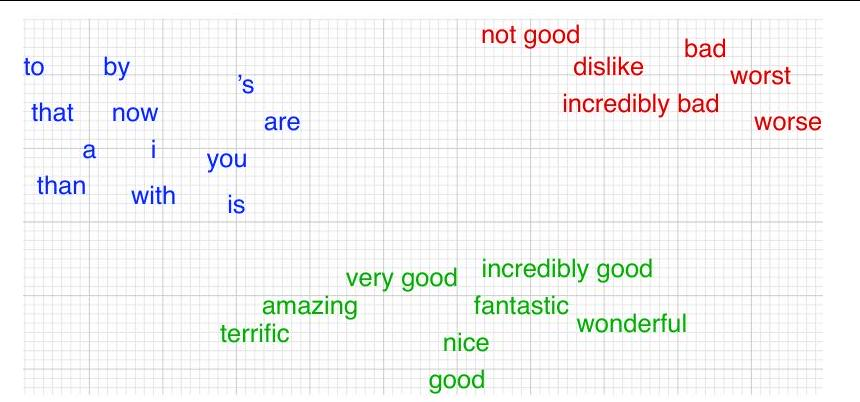
\includegraphics[max width=\textwidth, center]{2025_03_24_4f41283092a9d1f7a40eg-114}

Figure 6.1 A two-dimensional (t-SNE) projection of embeddings for some words and phrases, showing that words with similar meanings are nearby in space. The original $60-$ dimensional embeddings were trained for sentiment analysis. Simplified from Li et al. (2015) with colors added for explanation.

Fig. 6.1 shows a visualization of embeddings learned for sentiment analysis, showing the location of selected words projected down from 60-dimensional space into a two dimensional space. Notice the distinct regions containing positive words, negative words, and neutral function words.

The fine-grained model of word similarity of vector semantics offers enormous power to NLP applications. NLP applications like the sentiment classifiers of Chapter 4 or Chapter 5 depend on the same words appearing in the training and test sets. But by representing words as embeddings, a classifier can assign sentiment as long as it sees some words with similar meanings. And as we'll see, vector semantic models can be learned automatically from text without supervision.

In this chapter we'll introduce the two most commonly used models. In the tf-idf model, an important baseline, the meaning of a word is defined by a simple function of the counts of nearby words. We will see that this method results in very long vectors that are sparse, i.e. mostly zeros (since most words simply never occur in the context of others). We'll introduce the word2vec model family for constructing short, dense vectors that have useful semantic properties. We'll also introduce the cosine, the standard way to use embeddings to compute semantic similarity, between two words, two sentences, or two documents, an important tool in practical applications like question answering, summarization, or automatic essay grading.

\subsection*{6.3 Words and Vectors}
"The most important attributes of a vector in 3-space are \{Location, Location, Location\}" Randall Munroe, \href{https://xkcd.com/2358/}{https://xkcd.com/2358/}

Vector or distributional models of meaning are generally based on a co-occurrence matrix, a way of representing how often words co-occur. We'll look at two popular matrices: the term-document matrix and the term-term matrix.

\subsection*{6.3.1 Vectors and documents}
In a term-document matrix, each row represents a word in the vocabulary and each column represents a document from some collection of documents. Fig. 6.2 shows a small selection from a term-document matrix showing the occurrence of four words in four plays by Shakespeare. Each cell in this matrix represents the number of times\\
a particular word (defined by the row) occurs in a particular document (defined by the column). Thus fool appeared 58 times in Twelfth Night.

\begin{center}
\begin{tabular}{lcccc}
\hline
 & As You Like It & Twelfth Night & Julius Caesar & Henry V \\
\hline
battle & 1 & 0 & 7 & 13 \\
good & 114 & 80 & 62 & 89 \\
fool & 36 & 58 & 1 & 4 \\
wit & 20 & 15 & 2 & 3 \\
\hline
\end{tabular}
\end{center}

Figure 6.2 The term-document matrix for four words in four Shakespeare plays. Each cell contains the number of times the (row) word occurs in the (column) document.

The term-document matrix of Fig. 6.2 was first defined as part of the vector space model of information retrieval (Salton, 1971). In this model, a document is represented as a count vector, a column in Fig. 6.3.

To review some basic linear algebra, a vector is, at heart, just a list or array of numbers. So As You Like It is represented as the list $[1,114,36,20$ ] (the first column vector in Fig. 6.3) and Julius Caesar is represented as the list [7,62,1,2] (the third column vector). A vector space is a collection of vectors, and is characterized by its dimension. Vectors in a 3-dimensional vector space have an element for each dimension of the space. We will loosely refer to a vector in a 4-dimensional space as a 4-dimensional vector, with one element along each dimension. In the example in Fig. 6.3, we've chosen to make the document vectors of dimension 4, just so they fit on the page; in real term-document matrices, the document vectors would have dimensionality $|V|$, the vocabulary size.

The ordering of the numbers in a vector space indicates the different dimensions on which documents vary. The first dimension for both these vectors corresponds to the number of times the word battle occurs, and we can compare each dimension, noting for example that the vectors for As You Like It and Twelfth Night have similar values ( 1 and 0 , respectively) for the first dimension.

\begin{center}
\begin{tabular}{ccccc}
\hline
 & As You Like It & Twelfth Night & Julius Caesar & Henry V \\
\hline
battle & 1 & 14 & 0 & 7 \\
good & 36 & 58 & 62 & $\left(\begin{array}{c}13 \\ \text { fool } \\ \text { wit }\end{array}\right.$ \\
20 & 15 &  & 89 &  \\
\hline
\end{tabular}
\end{center}

Figure 6.3 The term-document matrix for four words in four Shakespeare plays. The red boxes show that each document is represented as a column vector of length four.

We can think of the vector for a document as a point in $|V|$-dimensional space; thus the documents in Fig. 6.3 are points in 4-dimensional space. Since 4-dimensional spaces are hard to visualize, Fig. 6.4 shows a visualization in two dimensions; we've arbitrarily chosen the dimensions corresponding to the words battle and fool.

Term-document matrices were originally defined as a means of finding similar documents for the task of document information retrieval. Two documents that are similar will tend to have similar words, and if two documents have similar words their column vectors will tend to be similar. The vectors for the comedies As You Like It $[1,114,36,20]$ and Twelfth Night $[0,80,58,15]$ look a lot more like each other (more fools and wit than battles) than they look like Julius Caesar [7,62,1,2] or Henry $V[13,89,4,3]$. This is clear with the raw numbers; in the first dimension (battle) the comedies have low numbers and the others have high numbers, and we can see it visually in Fig. 6.4; we'll see very shortly how to quantify this intuition more formally.\\
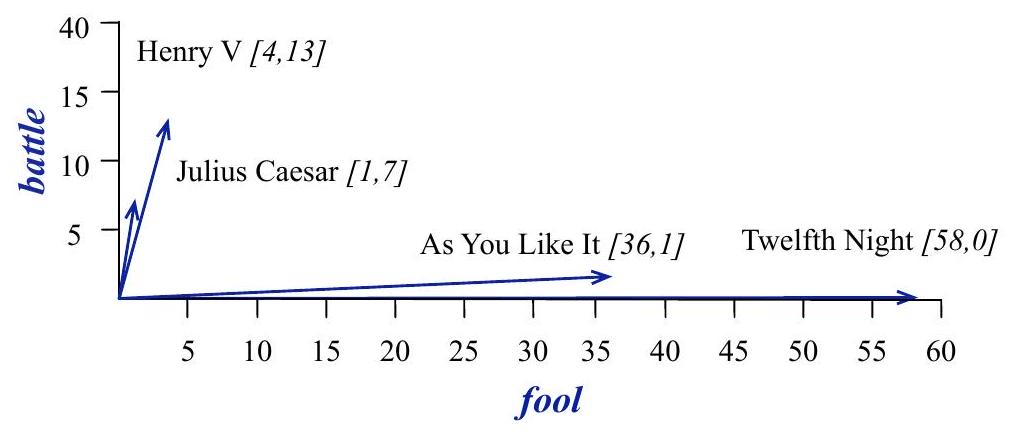
\includegraphics[max width=\textwidth, center]{2025_03_24_4f41283092a9d1f7a40eg-116}

Figure 6.4 A spatial visualization of the document vectors for the four Shakespeare play documents, showing just two of the dimensions, corresponding to the words battle and fool. The comedies have high values for the fool dimension and low values for the battle dimension.

A real term-document matrix, of course, wouldn't just have 4 rows and columns, let alone 2. More generally, the term-document matrix has $|V|$ rows (one for each word type in the vocabulary) and $D$ columns (one for each document in the collection); as we'll see, vocabulary sizes are generally in the tens of thousands, and the number of documents can be enormous (think about all the pages on the web).

Information retrieval (IR) is the task of finding the document $d$ from the $D$ documents in some collection that best matches a query $q$. For IR we'll therefore also represent a query by a vector, also of length $|V|$, and we'll need a way to compare two vectors to find how similar they are. (Doing IR will also require efficient ways to store and manipulate these vectors by making use of the convenient fact that these vectors are sparse, i.e., mostly zeros).

Later in the chapter we'll introduce some of the components of this vector comparison process: the tf-idf term weighting, and the cosine similarity metric.

\subsection*{6.3.2 Words as vectors: document dimensions}
We've seen that documents can be represented as vectors in a vector space. But vector semantics can also be used to represent the meaning of words. We do this by associating each word with a word vector- a row vector rather than a column vector, hence with different dimensions, as shown in Fig. 6.5. The four dimensions of the vector for fool, $[36,58,1,4]$, correspond to the four Shakespeare plays. Word counts in the same four dimensions are used to form the vectors for the other 3 words: wit, [20,15,2,3]; battle, [1,0,7,13]; and good [114,80,62,89].

\begin{center}
\begin{tabular}{ccccc}
\hline
 & As You Like It & Twelfth Night & Julius Caesar & Henry V \\
\hline
\begin{tabular}{c}
battle \\
good \\
fool \\
wit \\
\end{tabular} & 1 & 0 & 7 & 13 \\
\hline
\end{tabular}
\end{center}

Figure 6.5 The term-document matrix for four words in four Shakespeare plays. The red boxes show that each word is represented as a row vector of length four.

For documents, we saw that similar documents had similar vectors, because similar documents tend to have similar words. This same principle applies to words: similar words have similar vectors because they tend to occur in similar documents. The term-document matrix thus lets us represent the meaning of a word by the documents it tends to occur in.

\subsection*{6.3.3 Words as vectors: word dimensions}
An alternative to using the term-document matrix to represent words as vectors of document counts, is to use the term-term matrix, also called the word-word ma-\\
word-word matrix trix or the term-context matrix, in which the columns are labeled by words rather than documents. This matrix is thus of dimensionality $|V| \times|V|$ and each cell records the number of times the row (target) word and the column (context) word co-occur in some context in some training corpus. The context could be the document, in which case the cell represents the number of times the two words appear in the same document. It is most common, however, to use smaller contexts, generally a window around the word, for example of 4 words to the left and 4 words to the right, in which case the cell represents the number of times (in some training corpus) the column word occurs in such a $\pm 4$ word window around the row word. Here are four examples of words in their windows:

$$
\begin{aligned}
& \text { is traditionally followed by cherry } \text { pie, a traditional dessert } \\
& \text { often mixed, such as } \text { strawberry } \\
& \text { rhubarb pie. Apple pie }
\end{aligned}
$$

If we then take every occurrence of each word (say strawberry) and count the context words around it, we get a word-word co-occurrence matrix. Fig. 6.6 shows a simplified subset of the word-word co-occurrence matrix for these four words computed from the Wikipedia corpus (Davies, 2015).

\begin{center}
\begin{tabular}{ccccccccc}
\hline
 & aardvark & $\ldots$ & computer & data & result & pie & sugar & $\ldots$ \\
\hline
cherry & 0 & $\ldots$ & 2 & 8 & 9 & 442 & 25 & $\ldots$ \\
strawberry & 0 & $\ldots$ & 0 & 0 & 1 & 60 & 19 & $\ldots$ \\
digital & 0 & $\ldots$ & 1670 & 1683 & 85 & 5 & 4 & $\ldots$ \\
information & 0 & $\ldots$ & 3325 & 3982 & 378 & 5 & 13 & $\ldots$ \\
\hline
\end{tabular}
\end{center}

Figure 6.6 Co-occurrence vectors for four words in the Wikipedia corpus, showing six of the dimensions (hand-picked for pedagogical purposes). The vector for digital is outlined in red. Note that a real vector would have vastly more dimensions and thus be much sparser.

Note in Fig. 6.6 that the two words cherry and strawberry are more similar to each other (both pie and sugar tend to occur in their window) than they are to other words like digital; conversely, digital and information are more similar to each other than, say, to strawberry. Fig. 6.7 shows a spatial visualization.\\
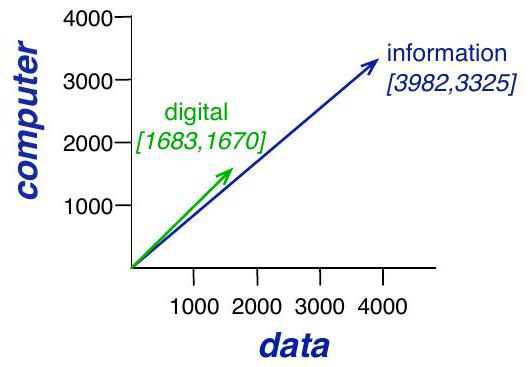
\includegraphics[max width=\textwidth, center]{2025_03_24_4f41283092a9d1f7a40eg-117}

Figure 6.7 A spatial visualization of word vectors for digital and information, showing just two of the dimensions, corresponding to the words data and computer.

Note that $|V|$, the dimensionality of the vector, is generally the size of the vocabulary, often between 10,000 and 50,000 words (using the most frequent words\\
in the training corpus; keeping words after about the most frequent 50,000 or so is generally not helpful). Since most of these numbers are zero these are sparse vector representations; there are efficient algorithms for storing and computing with sparse matrices.

Now that we have some intuitions, let's move on to examine the details of computing word similarity. Afterwards we'll discuss methods for weighting cells.

\subsection*{6.4 Cosine for measuring similarity}
dot product inner product\\
vector length

To measure similarity between two target words $v$ and $w$, we need a metric that takes two vectors (of the same dimensionality, either both with words as dimensions, hence of length $|V|$, or both with documents as dimensions, of length $|D|$ ) and gives a measure of their similarity. By far the most common similarity metric is the cosine of the angle between the vectors.

The cosine-like most measures for vector similarity used in NLP-is based on the dot product operator from linear algebra, also called the inner product:


\begin{equation*}
\operatorname{dot} \operatorname{product}(\mathbf{v}, \mathbf{w})=\mathbf{v} \cdot \mathbf{w}=\sum_{i=1}^{N} v_{i} w_{i}=v_{1} w_{1}+v_{2} w_{2}+\ldots+v_{N} w_{N} \tag{6.7}
\end{equation*}


The dot product acts as a similarity metric because it will tend to be high just when the two vectors have large values in the same dimensions. Alternatively, vectors that have zeros in different dimensions-orthogonal vectors-will have a dot product of 0 , representing their strong dissimilarity.

This raw dot product, however, has a problem as a similarity metric: it favors long vectors. The vector length is defined as


\begin{equation*}
|\mathbf{v}|=\sqrt{\sum_{i=1}^{N} v_{i}^{2}} \tag{6.8}
\end{equation*}


The dot product is higher if a vector is longer, with higher values in each dimension. More frequent words have longer vectors, since they tend to co-occur with more words and have higher co-occurrence values with each of them. The raw dot product thus will be higher for frequent words. But this is a problem; we'd like a similarity metric that tells us how similar two words are regardless of their frequency.

We modify the dot product to normalize for the vector length by dividing the dot product by the lengths of each of the two vectors. This normalized dot product turns out to be the same as the cosine of the angle between the two vectors, following from the definition of the dot product between two vectors $\mathbf{a}$ and $\mathbf{b}$ :


\begin{align*}
\mathbf{a} \cdot \mathbf{b} & =|\mathbf{a}||\mathbf{b}| \cos \theta \\
\frac{\mathbf{a} \cdot \mathbf{b}}{|\mathbf{a}||\mathbf{b}|} & =\cos \theta \tag{6.9}
\end{align*}


cosine $\quad$ The cosine similarity metric between two vectors $\mathbf{v}$ and $\mathbf{w}$ thus can be computed as:


\begin{equation*}
\operatorname{cosine}(\mathbf{v}, \mathbf{w})=\frac{\mathbf{v} \cdot \mathbf{w}}{|\mathbf{v} \| \mathbf{w}|}=\frac{\sum_{i=1}^{N} v_{i} w_{i}}{\sqrt{\sum_{i=1}^{N} v_{i}^{2}} \sqrt{\sum_{i=1}^{N} w_{i}^{2}}} \tag{6.10}
\end{equation*}


For some applications we pre-normalize each vector, by dividing it by its length, creating a unit vector of length 1 . Thus we could compute a unit vector from a by dividing it by $|\mathbf{a}|$. For unit vectors, the dot product is the same as the cosine.

The cosine value ranges from 1 for vectors pointing in the same direction, through 0 for orthogonal vectors, to -1 for vectors pointing in opposite directions. But since raw frequency values are non-negative, the cosine for these vectors ranges from 0-1.

Let's see how the cosine computes which of the words cherry or digital is closer in meaning to information, just using raw counts from the following shortened table:

\begin{center}
\begin{tabular}{cccc}
\hline
 & pie & data & computer \\
\hline
cherry & 442 & 8 & 2 \\
digital & 5 & 1683 & 1670 \\
information & 5 & 3982 & 3325 \\
\hline
\end{tabular}
\end{center}

$$
\begin{aligned}
& \cos (\text { cherry } \text {,information })=\frac{442 * 5+8 * 3982+2 * 3325}{\sqrt{442^{2}+8^{2}+2^{2}} \sqrt{5^{2}+3982^{2}+3325^{2}}}=.018 \\
& \cos (\text { digital,information })=\frac{5 * 5+1683 * 3982+1670 * 3325}{\sqrt{5^{2}+1683^{2}+1670^{2}} \sqrt{5^{2}+3982^{2}+3325^{2}}}=.996
\end{aligned}
$$

The model decides that information is way closer to digital than it is to cherry, a result that seems sensible. Fig. 6.8 shows a visualization.\\
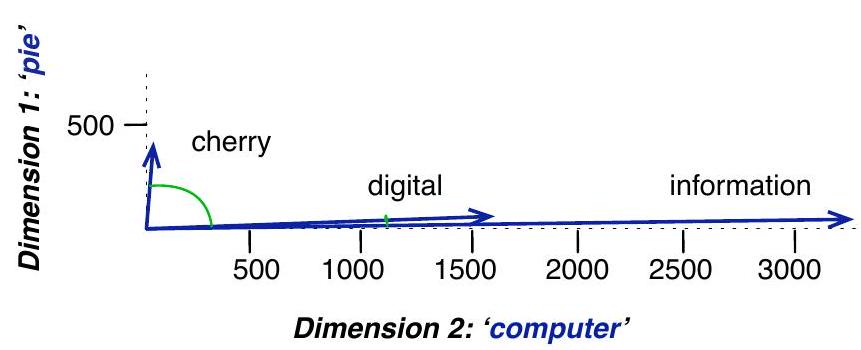
\includegraphics[max width=\textwidth, center]{2025_03_24_4f41283092a9d1f7a40eg-119}

Figure 6.8 A (rough) graphical demonstration of cosine similarity, showing vectors for three words (cherry, digital, and information) in the two dimensional space defined by counts of the words computer and pie nearby. The figure doesn't show the cosine, but it highlights the angles; note that the angle between digital and information is smaller than the angle between cherry and information. When two vectors are more similar, the cosine is larger but the angle is smaller; the cosine has its maximum (1) when the angle between two vectors is smallest $\left(0^{\circ}\right)$; the cosine of all other angles is less than 1.

\subsection*{6.5 TF-IDF: Weighing terms in the vector}
The co-occurrence matrices above represent each cell by frequencies, either of words with documents (Fig. 6.5), or words with other words (Fig. 6.6). But raw frequency\\
is not the best measure of association between words. Raw frequency is very skewed and not very discriminative. If we want to know what kinds of contexts are shared by cherry and strawberry but not by digital and information, we're not going to get good discrimination from words like the, it, or they, which occur frequently with all sorts of words and aren't informative about any particular word. We saw this also in Fig. 6.3 for the Shakespeare corpus; the dimension for the word good is not very discriminative between plays; good is simply a frequent word and has roughly equivalent high frequencies in each of the plays.

It's a bit of a paradox. Words that occur nearby frequently (maybe pie nearby cherry) are more important than words that only appear once or twice. Yet words that are too frequent-ubiquitous, like the or good- are unimportant. How can we balance these two conflicting constraints?

There are two common solutions to this problem: in this section we'll describe the tf-idf weighting, usually used when the dimensions are documents. In the next section we introduce the PPMI algorithm (usually used when the dimensions are words).

The tf-idf weighting (the '-' here is a hyphen, not a minus sign) is the product of two terms, each term capturing one of these two intuitions:

The first is the term frequency (Luhn, 1957): the frequency of the word $t$ in the document $d$. We can just use the raw count as the term frequency:


\begin{equation*}
\mathrm{tf}_{t, d}=\operatorname{count}(t, d) \tag{6.11}
\end{equation*}


More commonly we squash the raw frequency a bit, by using the $\log _{10}$ of the frequency instead. The intuition is that a word appearing 100 times in a document doesn't make that word 100 times more likely to be relevant to the meaning of the document. We also need to do something special with counts of 0 , since we can't take the $\log$ of $0 .^{2}$

\[
\mathrm{tf}_{t, d}= \begin{cases}1+\log _{10} \operatorname{count}(t, d) & \text { if } \operatorname{count}(t, d)>0  \tag{6.12}\\ 0 & \text { otherwise }\end{cases}
\]

If we use $\log$ weighting, terms which occur 0 times in a document would have $\mathrm{tf}=0$, 1 times in a document $\mathrm{tf}=1+\log _{10}(1)=1+0=1$, 10 times in a document $\mathrm{tf}=$ $1+\log _{10}(10)=2,100$ times $\mathrm{tf}=1+\log _{10}(100)=3,1000$ times $\mathrm{tf}=4$, and so on.

The second factor in tf -idf is used to give a higher weight to words that occur only in a few documents. Terms that are limited to a few documents are useful for discriminating those documents from the rest of the collection; terms that occur frequently across the entire collection aren't as helpful. The document frequency $\mathbf{d f}_{t}$ of a term $t$ is the number of documents it occurs in. Document frequency is not the same as the collection frequency of a term, which is the total number of times the word appears in the whole collection in any document. Consider in the collection of Shakespeare's 37 plays the two words Romeo and action. The words have identical collection frequencies (they both occur 113 times in all the plays) but very different document frequencies, since Romeo only occurs in a single play. If our goal is to find documents about the romantic tribulations of Romeo, the word Romeo should be highly weighted, but not action:

\begin{center}
\begin{tabular}{lll}
\hline
 & Collection Frequency & Document Frequency \\
Romeo & 113 & 1 \\
action & 113 & 31 \\
\hline
\end{tabular}
\end{center}

\footnotetext{2 We can also use this alternative formulation, which we have used in earlier editions: $\mathrm{tf}_{t, d}=$ $\log _{10}(\operatorname{count}(t, d)+1)$
}We emphasize discriminative words like Romeo via the inverse document frequency or idf term weight (Sparck Jones, 1972). The idf is defined using the fracthe number of documents in which term $t$ occurs. The fewer documents in which a term occurs, the higher this weight. The lowest weight of 1 is assigned to terms that occur in all the documents. It's usually clear what counts as a document: in Shakespeare we would use a play; when processing a collection of encyclopedia articles like Wikipedia, the document is a Wikipedia page; in processing newspaper articles, the document is a single article. Occasionally your corpus might not have appropriate document divisions and you might need to break up the corpus into documents yourself for the purposes of computing idf.

Because of the large number of documents in many collections, this measure too is usually squashed with a log function. The resulting definition for inverse document frequency (idf) is thus


\begin{equation*}
\operatorname{idf}_{t}=\log _{10}\left(\frac{N}{\mathrm{df}_{t}}\right) \tag{6.13}
\end{equation*}


Here are some idf values for some words in the Shakespeare corpus, (along with the document frequency df values on which they are based) ranging from extremely informative words which occur in only one play like Romeo, to those that occur in a few like salad or Falstaff, to those which are very common like fool or so common as to be completely non-discriminative since they occur in all 37 plays like good or sweet. ${ }^{3}$

\begin{center}
\begin{tabular}{lll}
\hline
Word & df & idf \\
\hline
Romeo & 1 & 1.57 \\
salad & 2 & 1.27 \\
Falstaff & 4 & 0.967 \\
forest & 12 & 0.489 \\
battle & 21 & 0.246 \\
wit & 34 & 0.037 \\
fool & 36 & 0.012 \\
good & 37 & 0 \\
sweet & 37 & 0 \\
\hline
\end{tabular}
\end{center}

The tf-idf weighted value $w_{t, d}$ for word $t$ in document $d$ thus combines term frequency $\mathrm{tf}_{t, d}$ (defined either by Eq. 6.11 or by Eq. 6.12) with idf from Eq. 6.13:


\begin{equation*}
w_{t, d}=\mathrm{tf}_{t, d} \times \operatorname{idf}_{t} \tag{6.14}
\end{equation*}


Fig. 6.9 applies tf-idf weighting to the Shakespeare term-document matrix in Fig. 6.2, using the tf equation Eq. 6.12. Note that the tf-idf values for the dimension corresponding to the word good have now all become 0 ; since this word appears in every document, the tf-idf weighting leads it to be ignored. Similarly, the word fool, which appears in 36 out of the 37 plays, has a much lower weight.

The tf-idf weighting is the way for weighting co-occurrence matrices in information retrieval, but also plays a role in many other aspects of natural language processing. It's also a great baseline, the simple thing to try first. We'll look at other weightings like PPMI (Positive Pointwise Mutual Information) in Section 6.6.

\footnotetext{3 Sweet was one of Shakespeare's favorite adjectives, a fact probably related to the increased use of sugar in European recipes around the turn of the 16th century (Jurafsky, 2014, p. 175).
}\begin{center}
\begin{tabular}{lllll}
\hline
 & As You Like It & Twelfth Night & Julius Caesar & Henry V \\
\hline
battle & 0.246 & 0 & 0.454 & 0.520 \\
good & 0 & 0 & 0 & 0 \\
fool & 0.030 & 0.033 & 0.0012 & 0.0019 \\
wit & 0.085 & 0.081 & 0.048 & 0.054 \\
\hline
\end{tabular}
\end{center}

Figure 6.9 A portion of the tf-idf weighted term-document matrix for four words in Shakespeare plays, showing a selection of 4 plays, using counts from Fig. 6.2. For example the 0.085 value for wit in As You Like It is the product of $\mathrm{tf}=1+\log _{10}(20)=2.301$ and idf $=.037$. Note that the idf weighting has eliminated the importance of the ubiquitous word good and vastly reduced the impact of the almost-ubiquitous word fool.

\subsection*{6.6 Pointwise Mutual Information (PMI)}
pointwise\\
pointwise information

An alternative weighting function to tf-idf, PPMI (positive pointwise mutual information), is used for term-term-matrices, when the vector dimensions correspond to words rather than documents. PPMI draws on the intuition that the best way to weigh the association between two words is to ask how much more the two words co-occur in our corpus than we would have a priori expected them to appear by chance.

Pointwise mutual information (Fano, 1961) ${ }^{4}$ is one of the most important concepts in NLP. It is a measure of how often two events $x$ and $y$ occur, compared with what we would expect if they were independent:


\begin{equation*}
I(x, y)=\log _{2} \frac{P(x, y)}{P(x) P(y)} \tag{6.16}
\end{equation*}


The pointwise mutual information between a target word $w$ and a context word $c$ (Church and Hanks 1989, Church and Hanks 1990) is then defined as:


\begin{equation*}
\operatorname{PMI}(w, c)=\log _{2} \frac{P(w, c)}{P(w) P(c)} \tag{6.17}
\end{equation*}


The numerator tells us how often we observed the two words together (assuming we compute probability by using the MLE). The denominator tells us how often we would expect the two words to co-occur assuming they each occurred independently; recall that the probability of two independent events both occurring is just the product of the probabilities of the two events. Thus, the ratio gives us an estimate of how much more the two words co-occur than we expect by chance. PMI is a useful tool whenever we need to find words that are strongly associated.

PMI values range from negative to positive infinity. But negative PMI values (which imply things are co-occurring less often than we would expect by chance) tend to be unreliable unless our corpora are enormous. To distinguish whether two words whose individual probability is each $10^{-6}$ occur together less often than chance, we would need to be certain that the probability of the two occurring together is significantly less than $10^{-12}$, and this kind of granularity would require an enormous corpus. Furthermore it's not clear whether it's even possible to evaluate such scores of 'unrelatedness' with human judgments. For this reason it is more

\footnotetext{4 PMI is based on the mutual information between two random variables $X$ and $Y$, defined as:


\begin{equation*}
I(X, Y)=\sum_{x} \sum_{y} P(x, y) \log _{2} \frac{P(x, y)}{P(x) P(y)} \tag{6.15}
\end{equation*}


In a confusion of terminology, Fano used the phrase mutual information to refer to what we now call pointwise mutual information and the phrase expectation of the mutual information for what we now call mutual information
}PPMI common to use Positive PMI (called PPMI) which replaces all negative PMI values with zero (Church and Hanks 1989, Dagan et al. 1993, Niwa and Nitta 1994) ${ }^{5}$ :


\begin{equation*}
\operatorname{PPMI}(w, c)=\max \left(\log _{2} \frac{P(w, c)}{P(w) P(c)}, 0\right) \tag{6.18}
\end{equation*}


More formally, let's assume we have a co-occurrence matrix F with W rows (words) and C columns (contexts), where $f_{i j}$ gives the number of times word $w_{i}$ occurs with context $c_{j}$. This can be turned into a PPMI matrix where $\mathrm{PPMI}_{i j}$ gives the PPMI value of word $w_{i}$ with context $c_{j}$ (which we can also express as $\operatorname{PPMI}\left(w_{i}, c_{j}\right)$ or $\operatorname{PPMI}(w=i, c=j))$ as follows:


\begin{gather*}
p_{i j}=\frac{f_{i j}}{\sum_{i=1}^{W} \sum_{j=1}^{C} f_{i j}}, \quad p_{i *}=\frac{\sum_{j=1}^{C} f_{i j}}{\sum_{i=1}^{W} \sum_{j=1}^{C} f_{i j}}, \quad p_{* j}=\frac{\sum_{i=1}^{W} f_{i j}}{\sum_{i=1}^{W} \sum_{j=1}^{C} f_{i j}}  \tag{6.19}\\
\operatorname{PPMI}_{i j}=\max \left(\log _{2} \frac{p_{i j}}{p_{i *} p_{* j}}, 0\right) \tag{6.20}
\end{gather*}


Let's see some PPMI calculations. We'll use Fig. 6.10, which repeats Fig. 6.6 plus all the count marginals, and let's pretend for ease of calculation that these are the only words/contexts that matter.

\begin{center}
\begin{tabular}{ccccccc}
\hline
 & computer & data & result & pie & sugar & count(w) \\
\hline
cherry & 2 & 8 & 9 & 442 & 25 & 486 \\
strawberry & 0 & 0 & 1 & 60 & 19 & 80 \\
\begin{tabular}{c}
digital \\
information \\
\end{tabular} & 1670 & 1683 & 85 & 5 & 4 & 3447 \\
 & 3325 & 3982 & 378 & 5 & 13 & 7703 \\
count(context) & 4997 & 5673 & 473 & 512 & 61 & 11716 \\
\hline
\end{tabular}
\end{center}

Figure 6.10 Co-occurrence counts for four words in 5 contexts in the Wikipedia corpus, together with the marginals, pretending for the purpose of this calculation that no other words/contexts matter.

Thus for example we could compute PPMI(information,data), assuming we pretended that Fig. 6.6 encompassed all the relevant word contexts/dimensions, as follows:

$$
\begin{aligned}
P(\mathrm{w}=\text { information, } \mathrm{c}=\text { data }) & =\frac{3982}{11716}=.3399 \\
P(\mathrm{w}=\text { information }) & =\frac{7703}{11716}=.6575 \\
P(\mathrm{c}=\text { data }) & =\frac{5673}{11716}=.4842 \\
\mathrm{PPMI}(\text { information,data }) & =\log _{2}(.3399 /(.6575 * .4842))=.0944
\end{aligned}
$$

Fig. 6.11 shows the joint probabilities computed from the counts in Fig. 6.10, and Fig. 6.12 shows the PPMI values. Not surprisingly, cherry and strawberry are highly associated with both pie and sugar, and data is mildly associated with information.

PMI has the problem of being biased toward infrequent events; very rare words tend to have very high PMI values. One way to reduce this bias toward low frequency

\footnotetext{5 Positive PMI also cleanly solves the problem of what to do with zero counts, using 0 to replace the $-\infty$ from $\log (0)$.
}\begin{center}
\begin{tabular}{lcccccc}
 & \multicolumn{6}{c}{$\mathbf{p ( w , c o n t e x t )}$} \\
\hline
 & computer & data & result & pie & sugar & $\mathbf{p ( w )}$ \\
\hline
cherry & 0.0002 & 0.0007 & 0.0008 & 0.0377 & 0.0021 & 0.0415 \\
strawberry & 0.0000 & 0.0000 & 0.0001 & 0.0051 & 0.0016 & 0.0068 \\
\begin{tabular}{c}
digital \\
information \\
\end{tabular} & 0.1425 & 0.1436 & 0.0073 & 0.0004 & 0.0003 & 0.2942 \\
 & 0.2838 & 0.3399 & 0.0323 & 0.0004 & 0.0011 & 0.6575 \\
p(context) & 0.4265 & 0.4842 & 0.0404 & 0.0437 & 0.0052 &  \\
\hline
\end{tabular}
\end{center}

Figure 6.11 Replacing the counts in Fig. 6.6 with joint probabilities, showing the marginals in the right column and the bottom row.

\begin{center}
\begin{tabular}{cccccc}
\hline
 & computer & data & result & pie & sugar \\
\hline
cherry & 0 & 0 & 0 & 4.38 & 3.30 \\
strawberry & 0 & 0 & 0 & 4.10 & 5.51 \\
digital & 0.18 & 0.01 & 0 & 0 & 0 \\
information & 0.02 & 0.09 & 0.28 & 0 & 0 \\
\hline
\end{tabular}
\end{center}

Figure 6.12 The PPMI matrix showing the association between words and context words, computed from the counts in Fig. 6.11. Note that most of the 0 PPMI values are ones that had a negative PMI; for example $\operatorname{PMI}($ cherry, computer $)=-6.7$, meaning that cherry and computer co-occur on Wikipedia less often than we would expect by chance, and with PPMI we replace negative values by zero.\\
events is to slightly change the computation for $P(c)$, using a different function $P_{\alpha}(c)$ that raises the probability of the context word to the power of $\alpha$ :


\begin{align*}
\operatorname{PPMI}_{\alpha}(w, c) & =\max \left(\log _{2} \frac{P(w, c)}{P(w) P_{\alpha}(c)}, 0\right)  \tag{6.21}\\
P_{\alpha}(c) & =\frac{\operatorname{count}(c)^{\alpha}}{\sum_{c} \operatorname{count}(c)^{\alpha}} \tag{6.22}
\end{align*}


Levy et al. (2015) found that a setting of $\alpha=0.75$ improved performance of embeddings on a wide range of tasks (drawing on a similar weighting used for skipgrams described below in Eq. 6.32). This works because raising the count to $\alpha=$ 0.75 increases the probability assigned to rare contexts, and hence lowers their PMI ( $P_{\alpha}(c)>P(c)$ when $c$ is rare).

Another possible solution is Laplace smoothing: Before computing PMI, a small constant $k$ (values of $0.1-3$ are common) is added to each of the counts, shrinking (discounting) all the non-zero values. The larger the $k$, the more the non-zero counts are discounted.

\subsection*{6.7 Applications of the tf-idf or PPMI vector models}
In summary, the vector semantics model we've described so far represents a target word as a vector with dimensions corresponding either to the documents in a large collection (the term-document matrix) or to the counts of words in some neighboring window (the term-term matrix). The values in each dimension are counts, weighted by tf -idf (for term-document matrices) or PPMI (for term-term matrices), and the vectors are sparse (since most values are zero).

The model computes the similarity between two words $x$ and $y$ by taking the cosine of their tf-idf or PPMI vectors; high cosine, high similarity. This entire model\\
is sometimes referred to as the $\mathbf{t}$-idf model or the PPMI model, after the weighting function.

The tf-idf model of meaning is often used for document functions like deciding if two documents are similar. We represent a document by taking the vectors of all the words in the document, and computing the centroid of all those vectors. The centroid is the multidimensional version of the mean; the centroid of a set of vectors is a single vector that has the minimum sum of squared distances to each of the vectors in the set. Given $k$ word vectors $w_{1}, w_{2}, \ldots, w_{k}$, the centroid document vector $d$ is:


\begin{equation*}
d=\frac{w_{1}+w_{2}+\ldots+w_{k}}{k} \tag{6.23}
\end{equation*}


Given two documents, we can then compute their document vectors $d_{1}$ and $d_{2}$, and estimate the similarity between the two documents by $\cos \left(d_{1}, d_{2}\right)$. Document similarity is also useful for all sorts of applications; information retrieval, plagiarism detection, news recommender systems, and even for digital humanities tasks like comparing different versions of a text to see which are similar to each other.

Either the PPMI model or the tf-idf model can be used to compute word similarity, for tasks like finding word paraphrases, tracking changes in word meaning, or automatically discovering meanings of words in different corpora. For example, we can find the 10 most similar words to any target word $w$ by computing the cosines between $w$ and each of the $V-1$ other words, sorting, and looking at the top 10 .

\subsection*{6.8 Word2vec}
In the previous sections we saw how to represent a word as a sparse, long vector with dimensions corresponding to words in the vocabulary or documents in a collection. We now introduce a more powerful word representation: embeddings, short dense vectors. Unlike the vectors we've seen so far, embeddings are short, with number of dimensions $d$ ranging from 50-1000, rather than the much larger vocabulary size $|V|$ or number of documents $D$ we've seen. These $d$ dimensions don't have a clear interpretation. And the vectors are dense: instead of vector entries being sparse, mostly-zero counts or functions of counts, the values will be real-valued numbers that can be negative.

It turns out that dense vectors work better in every NLP task than sparse vectors. While we don't completely understand all the reasons for this, we have some intuitions. Representing words as 300-dimensional dense vectors requires our classifiers to learn far fewer weights than if we represented words as 50,000-dimensional vectors, and the smaller parameter space possibly helps with generalization and avoiding overfitting. Dense vectors may also do a better job of capturing synonymy. For example, in a sparse vector representation, dimensions for synonyms like car and automobile dimension are distinct and unrelated; sparse vectors may thus fail to capture the similarity between a word with car as a neighbor and a word with automobile as a neighbor.

In this section we introduce one method for computing embeddings: skip-gram with negative sampling, sometimes called SGNS. The skip-gram algorithm is one of two algorithms in a software package called word2vec, and so sometimes the algorithm is loosely referred to as word2vec (Mikolov et al. 2013a, Mikolov et al. 2013b). The word2vec methods are fast, efficient to train, and easily available on-\\
static\\
embeddings\\
line with code and pretrained embeddings. Word2vec embeddings are static embeddings, meaning that the method learns one fixed embedding for each word in the vocabulary. In Chapter 11 we'll introduce methods for learning dynamic contextual embeddings like the popular family of BERT representations, in which the vector for each word is different in different contexts.

The intuition of word2 vec is that instead of counting how often each word $w$ occurs near, say, apricot, we'll instead train a classifier on a binary prediction task: "Is word $w$ likely to show up near apricot?" We don't actually care about this prediction task; instead we'll take the learned classifier weights as the word embeddings.

The revolutionary intuition here is that we can just use running text as implicitly supervised training data for such a classifier; a word $c$ that occurs near the target word apricot acts as gold 'correct answer' to the question "Is word $c$ likely to show up near apricot?" This method, often called self-supervision, avoids the need for any sort of hand-labeled supervision signal. This idea was first proposed in the task of neural language modeling, when Bengio et al. (2003) and Collobert et al. (2011) showed that a neural language model (a neural network that learned to predict the next word from prior words) could just use the next word in running text as its supervision signal, and could be used to learn an embedding representation for each word as part of doing this prediction task.

We'll see how to do neural networks in the next chapter, but word2vec is a much simpler model than the neural network language model, in two ways. First, word2vec simplifies the task (making it binary classification instead of word prediction). Second, word2vec simplifies the architecture (training a logistic regression classifier instead of a multi-layer neural network with hidden layers that demand more sophisticated training algorithms). The intuition of skip-gram is:

\begin{enumerate}
  \item Treat the target word and a neighboring context word as positive examples.
  \item Randomly sample other words in the lexicon to get negative samples.
  \item Use logistic regression to train a classifier to distinguish those two cases.
  \item Use the learned weights as the embeddings.
\end{enumerate}

\subsection*{6.8.1 The classifier}
Let's start by thinking about the classification task, and then turn to how to train. Imagine a sentence like the following, with a target word apricot, and assume we're using a window of $\pm 2$ context words:

\begin{verbatim}
... lemon, a [tablespoon of apricot jam, a] pinch ...
    c1 c2 w c3 c4
\end{verbatim}

Our goal is to train a classifier such that, given a tuple $(w, c)$ of a target word $w$ paired with a candidate context word $c$ (for example (apricot, jam), or perhaps (apricot, aardvark)) it will return the probability that $c$ is a real context word (true for jam, false for aardvark):


\begin{equation*}
P(+\mid w, c) \tag{6.24}
\end{equation*}


The probability that word $c$ is not a real context word for $w$ is just 1 minus Eq. 6.24:


\begin{equation*}
P(-\mid w, c)=1-P(+\mid w, c) \tag{6.25}
\end{equation*}


How does the classifier compute the probability $P$ ? The intuition of the skipgram model is to base this probability on embedding similarity: a word is likely to occur near the target if its embedding vector is similar to the target embedding. To compute similarity between these dense embeddings, we rely on the intuition that two vectors are similar if they have a high dot product (after all, cosine is just a normalized dot product). In other words:


\begin{equation*}
\operatorname{Similarity}(w, c) \approx \mathbf{c} \cdot \mathbf{w} \tag{6.26}
\end{equation*}


The dot product $\mathbf{c} \cdot \mathbf{w}$ is not a probability, it's just a number ranging from $-\infty$ to $\infty$ (since the elements in word2vec embeddings can be negative, the dot product can be negative). To turn the dot product into a probability, we'll use the logistic or sigmoid function $\sigma(x)$, the fundamental core of logistic regression:


\begin{equation*}
\sigma(x)=\frac{1}{1+\exp (-x)} \tag{6.27}
\end{equation*}


We model the probability that word $c$ is a real context word for target word $w$ as:


\begin{equation*}
P(+\mid w, c)=\sigma(\mathbf{c} \cdot \mathbf{w})=\frac{1}{1+\exp (-\mathbf{c} \cdot \mathbf{w})} \tag{6.28}
\end{equation*}


The sigmoid function returns a number between 0 and 1, but to make it a probability we'll also need the total probability of the two possible events ( $c$ is a context word, and $c$ isn't a context word) to sum to 1 . We thus estimate the probability that word $c$ is not a real context word for $w$ as:


\begin{align*}
P(-\mid w, c) & =1-P(+\mid w, c) \\
& =\sigma(-\mathbf{c} \cdot \mathbf{w})=\frac{1}{1+\exp (\mathbf{c} \cdot \mathbf{w})} \tag{6.29}
\end{align*}


Equation 6.28 gives us the probability for one word, but there are many context words in the window. Skip-gram makes the simplifying assumption that all context words are independent, allowing us to just multiply their probabilities:


\begin{align*}
P\left(+\mid w, c_{1: L}\right) & =\prod_{i=1}^{L} \sigma\left(\mathbf{c}_{\mathbf{i}} \cdot \mathbf{w}\right)  \tag{6.30}\\
\log P\left(+\mid w, c_{1: L}\right) & =\sum_{i=1}^{L} \log \sigma\left(\mathbf{c}_{\mathbf{i}} \cdot \mathbf{w}\right) \tag{6.31}
\end{align*}


In summary, skip-gram trains a probabilistic classifier that, given a test target word $w$ and its context window of $L$ words $c_{1: L}$, assigns a probability based on how similar this context window is to the target word. The probability is based on applying the logistic (sigmoid) function to the dot product of the embeddings of the target word with each context word. To compute this probability, we just need embeddings for each target word and context word in the vocabulary.

Fig. 6.13 shows the intuition of the parameters we'll need. Skip-gram actually stores two embeddings for each word, one for the word as a target, and one for the word considered as context. Thus the parameters we need to learn are two matrices $\mathbf{W}$ and $\mathbf{C}$, each containing an embedding for every one of the $|V|$ words in the vocabulary $V .{ }^{6}$ Let's now turn to learning these embeddings (which is the real goal of training this classifier in the first place).

\footnotetext{6 In principle the target matrix and the context matrix could use different vocabularies, but we'll simplify by assuming one shared vocabulary $V$.
}
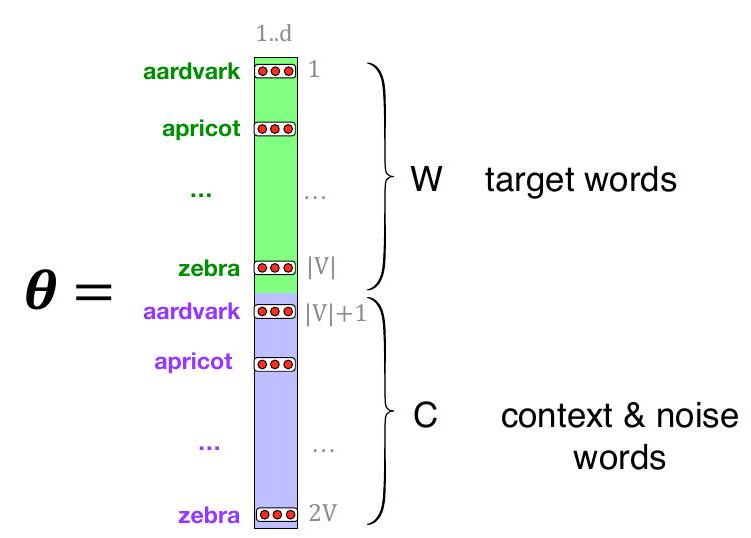
\includegraphics[max width=\textwidth, center]{2025_03_24_4f41283092a9d1f7a40eg-128}

Figure 6.13 The embeddings learned by the skipgram model. The algorithm stores two embeddings for each word, the target embedding (sometimes called the input embedding) and the context embedding (sometimes called the output embedding). The parameter $\theta$ that the algorithm learns is thus a matrix of $2|V|$ vectors, each of dimension $d$, formed by concatenating two matrices, the target embeddings $\mathbf{W}$ and the context+noise embeddings $\mathbf{C}$.

\subsection*{6.8.2 Learning skip-gram embeddings}
The learning algorithm for skip-gram embeddings takes as input a corpus of text, and a chosen vocabulary size N . It begins by assigning a random embedding vector for each of the N vocabulary words, and then proceeds to iteratively shift the embedding of each word $w$ to be more like the embeddings of words that occur nearby in texts, and less like the embeddings of words that don't occur nearby. Let's start by considering a single piece of training data:

\begin{verbatim}
... lemon, a [tablespoon of apricot jam, a] pinch ...
    c1 c2 w c3 c4
\end{verbatim}

This example has a target word $w$ (apricot), and 4 context words in the $L= \pm 2$ window, resulting in 4 positive training instances (on the left below):

\begin{center}
\begin{tabular}{l}
positive examples + \\
$w \quad c_{\text {pos }}$ \\
\hline
apricot tablespoon \\
apricot of \\
apricot \\
jam \\
apricot \\
a \\
\end{tabular}
\end{center}

negative examples -

\begin{center}
\begin{tabular}{llll}
$w$ & $c_{\text {neg }}$ & $w$ & $c_{\text {neg }}$ \\
\hline
apricot & aardvark & apricot & seven \\
apricot & my & apricot & forever \\
apricot & where & apricot & dear \\
apricot & coaxial & apricot if &  \\
\end{tabular}
\end{center}

For training a binary classifier we also need negative examples. In fact skipgram with negative sampling (SGNS) uses more negative examples than positive examples (with the ratio between them set by a parameter $k$ ). So for each of these ( $w, c_{p o s}$ ) training instances we'll create $k$ negative samples, each consisting of the target $w$ plus a 'noise word' $c_{n e g}$. A noise word is a random word from the lexicon, constrained not to be the target word $w$. The right above shows the setting where $k=2$, so we'll have 2 negative examples in the negative training set - for each positive example $w, c_{p o s}$.

The noise words are chosen according to their weighted unigram frequency $p_{\alpha}(w)$, where $\alpha$ is a weight. If we were sampling according to unweighted frequency $p(w)$, it would mean that with unigram probability $p$ ("the") we would choose the word the as a noise word, with unigram probability $p$ ("aardvark") we would\\
choose aardvark, and so on. But in practice it is common to set $\alpha=0.75$, i.e. use the weighting $p_{\frac{3}{4}}(w)$ :


\begin{equation*}
P_{\alpha}(w)=\frac{\operatorname{count}(w)^{\alpha}}{\sum_{w^{\prime}} \operatorname{count}\left(w^{\prime}\right)^{\alpha}} \tag{6.32}
\end{equation*}


Setting $\alpha=.75$ gives better performance because it gives rare noise words slightly higher probability: for rare words, $P_{\alpha}(w)>P(w)$. To illustrate this intuition, it might help to work out the probabilities for an example with $\alpha=.75$ and two events, $P(a)=0.99$ and $P(b)=0.01$ :


\begin{align*}
P_{\alpha}(a) & =\frac{.99^{.75}}{.99 .75+.01 .75}=0.97 \\
P_{\alpha}(b) & =\frac{.01^{.75}}{.99 .75+.01^{.75}}=0.03 \tag{6.33}
\end{align*}


Thus using $\alpha=.75$ increases the probability of the rare event $b$ from 0.01 to 0.03 .\\
Given the set of positive and negative training instances, and an initial set of embeddings, the goal of the learning algorithm is to adjust those embeddings to

\begin{itemize}
  \item Maximize the similarity of the target word, context word pairs ( $w, c_{p o s}$ ) drawn from the positive examples
  \item Minimize the similarity of the $\left(w, c_{n e g}\right)$ pairs from the negative examples.
\end{itemize}

If we consider one word/context pair ( $w, c_{\text {pos }}$ ) with its $k$ noise words $c_{n e g_{1}} \ldots c_{n e g_{k}}$, we can express these two goals as the following loss function $L$ to be minimized (hence the -); here the first term expresses that we want the classifier to assign the real context word $c_{p o s}$ a high probability of being a neighbor, and the second term expresses that we want to assign each of the noise words $c_{n e g_{i}}$ a high probability of being a non-neighbor, all multiplied because we assume independence:


\begin{align*}
L & =-\log \left[P\left(+\mid w, c_{p o s}\right) \prod_{i=1}^{k} P\left(-\mid w, c_{n e g_{i}}\right)\right] \\
& =-\left[\log P\left(+\mid w, c_{p o s}\right)+\sum_{i=1}^{k} \log P\left(-\mid w, c_{n e g_{i}}\right)\right] \\
& =-\left[\log P\left(+\mid w, c_{p o s}\right)+\sum_{i=1}^{k} \log \left(1-P\left(+\mid w, c_{n e g_{i}}\right)\right)\right] \\
& =-\left[\log \sigma\left(c_{p o s} \cdot w\right)+\sum_{i=1}^{k} \log \sigma\left(-c_{\text {neg }_{i}} \cdot w\right)\right] \tag{6.34}
\end{align*}


That is, we want to maximize the dot product of the word with the actual context words, and minimize the dot products of the word with the $k$ negative sampled nonneighbor words.

We minimize this loss function using stochastic gradient descent. Fig. 6.14 shows the intuition of one step of learning.

To get the gradient, we need to take the derivative of Eq. 6.34 with respect to the different embeddings. It turns out the derivatives are the following (we leave the\\
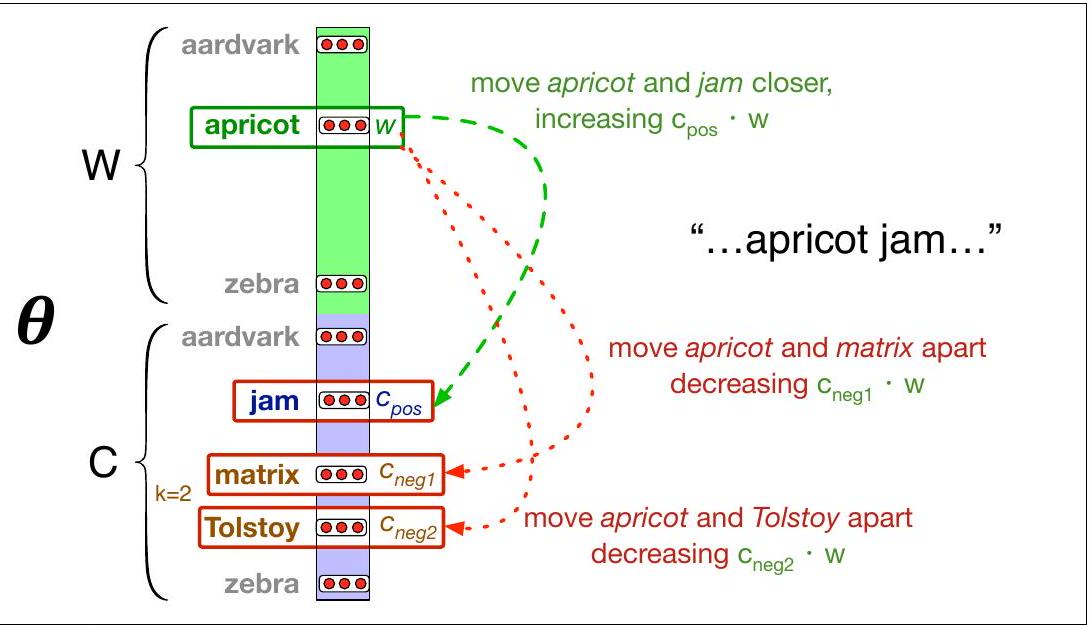
\includegraphics[max width=\textwidth, center]{2025_03_24_4f41283092a9d1f7a40eg-130}

Figure 6.14 Intuition of one step of gradient descent. The skip-gram model tries to shift embeddings so the target embeddings (here for apricot) are closer to (have a higher dot product with) context embeddings for nearby words (here jam) and further from (lower dot product with) context embeddings for noise words that don't occur nearby (here Tolstoy and matrix).\\
proof as an exercise at the end of the chapter):


\begin{align*}
\frac{\partial L}{\partial c_{p o s}} & =\left[\sigma\left(\mathbf{c}_{p o s} \cdot \mathbf{w}\right)-1\right] \mathbf{w}  \tag{6.35}\\
\frac{\partial L}{\partial c_{n e g}} & =\left[\sigma\left(\mathbf{c}_{n e g} \cdot \mathbf{w}\right)\right] \mathbf{w}  \tag{6.36}\\
\frac{\partial L}{\partial w} & =\left[\sigma\left(\mathbf{c}_{p o s} \cdot \mathbf{w}\right)-1\right] \mathbf{c}_{p o s}+\sum_{i=1}^{k}\left[\sigma\left(\mathbf{c}_{n e g_{i}} \cdot \mathbf{w}\right)\right] \mathbf{c}_{n e g_{i}} \tag{6.37}
\end{align*}


The update equations going from time step $t$ to $t+1$ in stochastic gradient descent are thus:


\begin{align*}
& \mathbf{c}_{p o s}^{t+1}=\mathbf{c}_{p o s}^{t}-\eta\left[\sigma\left(\mathbf{c}_{p o s}^{t} \cdot \mathbf{w}^{t}\right)-1\right] \mathbf{w}^{t}  \tag{6.38}\\
& \mathbf{c}_{\text {neg }}^{t+1}=\mathbf{c}_{\text {neg }}^{t}-\eta\left[\sigma\left(\mathbf{c}_{\text {neg }}^{t} \cdot \mathbf{w}^{t}\right)\right] \mathbf{w}^{t}  \tag{6.39}\\
& \mathbf{w}^{t+1}=\mathbf{w}^{t}-\eta\left[\left[\sigma\left(\mathbf{c}_{p o s}^{t} \cdot \mathbf{w}^{t}\right)-1\right] \mathbf{c}_{p o s}^{t}+\sum_{i=1}^{k}\left[\sigma\left(\mathbf{c}_{\text {neg }_{i}}^{t} \cdot \mathbf{w}^{t}\right)\right] \mathbf{c}_{n e g_{i}}^{t}\right] \tag{6.40}
\end{align*}


Just as in logistic regression, then, the learning algorithm starts with randomly initialized $\mathbf{W}$ and $\mathbf{C}$ matrices, and then walks through the training corpus using gradient descent to move $\mathbf{W}$ and $\mathbf{C}$ so as to minimize the loss in Eq. 6.34 by making the updates in (Eq. 6.38)-(Eq. 6.40).

Recall that the skip-gram model learns two separate embeddings for each word $i$ :\\
target matrix $\mathbf{W}$ and the context matrix $\mathbf{C}$. It's common to just add them together, representing word $i$ with the vector $\mathbf{w}_{i}+\mathbf{c}_{i}$. Alternatively we can throw away the $\mathbf{C}$ matrix and just represent each word $i$ by the vector $\mathbf{w}_{i}$.

As with the simple count-based methods like tf-idf, the context window size $L$ affects the performance of skip-gram embeddings, and experiments often tune the parameter $L$ on a devset.

\subsection*{6.8.3 Other kinds of static embeddings}
fasttext There are many kinds of static embeddings. An extension of word2vec, fasttext (Bojanowski et al., 2017), addresses a problem with word2vec as we have presented it so far: it has no good way to deal with unknown words-words that appear in a test corpus but were unseen in the training corpus. A related problem is word sparsity, such as in languages with rich morphology, where some of the many forms for each noun and verb may only occur rarely. Fasttext deals with these problems by using subword models, representing each word as itself plus a bag of constituent n-grams, with special boundary symbols $<$ and $>$ added to each word. For example, with $n=3$ the word where would be represented by the sequence $<$ where $>$ plus the character n -grams:

\begin{verbatim}
<wh, whe, her, ere, re>
\end{verbatim}

Then a skipgram embedding is learned for each constituent n -gram, and the word where is represented by the sum of all of the embeddings of its constituent n-grams. Unknown words can then be presented only by the sum of the constituent $n$-grams. A fasttext open-source library, including pretrained embeddings for 157 languages, is available at \href{https://fasttext.cc}{https://fasttext.cc}.

Another very widely used static embedding model is GloVe (Pennington et al., 2014), short for Global Vectors, because the model is based on capturing global corpus statistics. GloVe is based on ratios of probabilities from the word-word cooccurrence matrix, combining the intuitions of count-based models like PPMI while also capturing the linear structures used by methods like word2vec.

It turns out that dense embeddings like word2vec actually have an elegant mathematical relationship with sparse embeddings like PPMI, in which word2vec can be seen as implicitly optimizing a function of a PPMI matrix (Levy and Goldberg, 2014c).

\subsection*{6.9 Visualizing Embeddings}
\section*{"I see well in many dimensions as long as the dimensions are around two." The late economist Martin Shubik}
Visualizing embeddings is an important goal in helping understand, apply, and improve these models of word meaning. But how can we visualize a (for example) 100-dimensional vector?\\
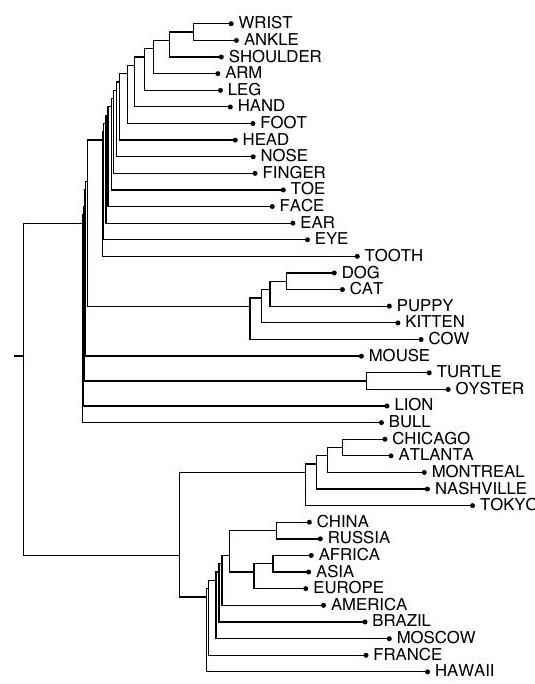
\includegraphics[max width=\textwidth, center]{2025_03_24_4f41283092a9d1f7a40eg-131}

The simplest way to visualize the meaning of a word $w$ embedded in a space is to list the most similar words to $w$ by sorting the vectors for all words in the vocabulary by their cosine with the vector for $w$. For example the 7 closest words to frog using a particular embeddings computed with the GloVe algorithm are: frogs, toad, litoria, leptodactylidae, rana, lizard, and eleutherodactylus (Pennington et al., 2014).

Yet another visualization method is to use a clustering algorithm to show a hierarchical representation of which words are similar to others in the embedding space. The uncaptioned figure on the left uses hierarchical clustering of some embedding vectors for nouns as a visualization\\
method (Rohde et al., 2006).\\
Probably the most common visualization method, how-\\
ever, is to project the 100 dimensions of a word down into 2\\
dimensions. Fig. 6.1 showed one such visualization, as does\\
Fig. 6.16, using a projection method called t-SNE (van der Maaten and Hinton, 2008).

\subsection*{6.10 Semantic properties of embeddings}
In this section we briefly summarize some of the semantic properties of embeddings that have been studied.

Different types of similarity or association: One parameter of vector semantic models that is relevant to both sparse PPMI vectors and dense word2vec vectors is the size of the context window used to collect counts. This is generally between 1 and 10 words on each side of the target word (for a total context of 2-20 words).

The choice depends on the goals of the representation. Shorter context windows tend to lead to representations that are a bit more syntactic, since the information is coming from immediately nearby words. When the vectors are computed from short context windows, the most similar words to a target word $w$ tend to be semantically similar words with the same parts of speech. When vectors are computed from long context windows, the highest cosine words to a target word $w$ tend to be words that are topically related but not similar.

For example Levy and Goldberg (2014a) showed that using skip-gram with a window of $\pm 2$, the most similar words to the word Hogwarts (from the Harry Potter series) were names of other fictional schools: Sunnydale (from Buffy the Vampire Slayer) or Evernight (from a vampire series). With a window of $\pm 5$, the most similar words to Hogwarts were other words topically related to the Harry Potter series: Dumbledore, Malfoy, and half-blood.

It's also often useful to distinguish two kinds of similarity or association between\\
first-order co-occurrence\\
second-order co-occurrence words (Schütze and Pedersen, 1993). Two words have first-order co-occurrence (sometimes called syntagmatic association) if they are typically nearby each other. Thus wrote is a first-order associate of book or poem. Two words have second-order co-occurrence (sometimes called paradigmatic association) if they have similar neighbors. Thus wrote is a second-order associate of words like said or remarked.

Analogy/Relational Similarity: Another semantic property of embeddings is their ability to capture relational meanings. In an important early vector space model of cognition, Rumelhart and Abrahamson (1973) proposed the parallelogram model for solving simple analogy problems of the form $a$ is to $b$ as $a^{*}$ is to what?. In such problems, a system is given a problem like apple:tree::grape:?, i.e., apple is to tree as grape is to $\qquad$ and must fill in the word vine. In the parallelogram model, illustrated in Fig. 6.15, the vector from the word apple to the word tree (= $\overrightarrow{\text { tree }}-\overrightarrow{\text { apple }}$ ) is added to the vector for grape ( $\overrightarrow{\text { grape }}$ ); the nearest word to that point is returned.

In early work with sparse embeddings, scholars showed that sparse vector models of meaning could solve such analogy problems (Turney and Littman, 2005), but the parallelogram method received more modern attention because of its success with word2vec or GloVe vectors (Mikolov et al. 2013c, Levy and Goldberg 2014b, Pennington et al. 2014). For example, the result of the expression $\overrightarrow{\mathrm{king}}-$\\
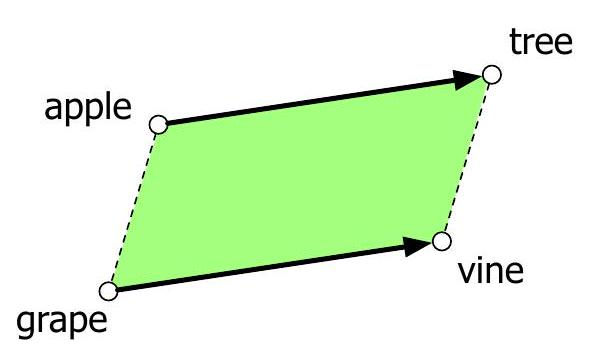
\includegraphics[max width=\textwidth, center]{2025_03_24_4f41283092a9d1f7a40eg-133(1)}

Figure 6.15 The parallelogram model for analogy problems (Rumelhart and Abrahamson, 1973): the location of $\overrightarrow{~ v i n e ~ c a n ~ b e ~ f o u n d ~ b y ~ s u b t r a c t i n g ~} \overrightarrow{\overrightarrow{p p l e}}$ from tree and adding grape.\\
$\overrightarrow{\mathrm{man}}+\overrightarrow{\text { woman }}$ is a vector close to $\overrightarrow{\text { queen }}$. Similarly, $\overrightarrow{\text { Paris }}-\overrightarrow{\text { France }}+\overrightarrow{\text { Italy results }}$ in a vector that is close to $\overrightarrow{\text { Rome }}$. The embedding model thus seems to be extracting representations of relations like MALE-FEMALE, or CAPITAL-CITY-OF, or even comparative/superlative, as shown in Fig. 6.16 from GloVe.\\
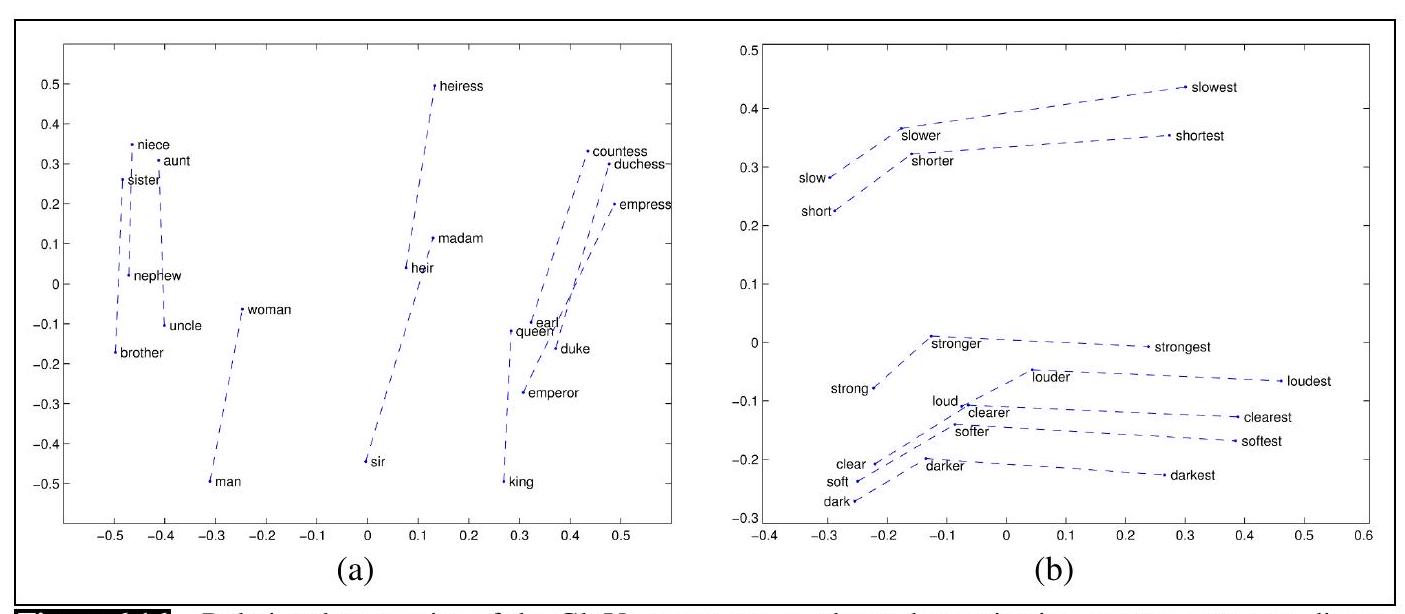
\includegraphics[max width=\textwidth, center]{2025_03_24_4f41283092a9d1f7a40eg-133}

Figure 6.16 Relational properties of the GloVe vector space, shown by projecting vectors onto two dimensions. (a) $\overrightarrow{\text { king }}-\overrightarrow{\mathrm{man}}+\overrightarrow{\text { woman }}$ is close to $\overrightarrow{\text { queen. (b) offsets seem to capture comparative and superlative }}$ morphology (Pennington et al., 2014).

For a $\mathbf{a}: \mathbf{b}:: \mathbf{a}^{*}: \mathbf{b}^{*}$ problem, meaning the algorithm is given vectors $\mathbf{a}, \mathbf{b}$, and $\mathbf{a}^{*}$ and must find $\mathbf{b}^{*}$, the parallelogram method is thus:


\begin{equation*}
\hat{\mathbf{b}}^{*}=\underset{\mathbf{x}}{\operatorname{argmin}} \operatorname{distance}\left(\mathbf{x}, \mathbf{b}-\mathbf{a}+\mathbf{a}^{*}\right) \tag{6.41}
\end{equation*}


with some distance function, such as Euclidean distance.\\
There are some caveats. For example, the closest value returned by the parallelogram algorithm in word2vec or GloVe embedding spaces is usually not in fact $\mathrm{b}^{*}$ but one of the 3 input words or their morphological variants (i.e., cherry:red $::$ potato:x returns potato or potatoes instead of brown), so these must be explicitly excluded. Furthermore while embedding spaces perform well if the task involves frequent words, small distances, and certain relations (like relating countries with their capitals or verbs/nouns with their inflected forms), the parallelogram method with embeddings doesn't work as well for other relations (Linzen 2016, Gladkova et al. 2016, Schluter 2018, Ethayarajh et al. 2019a), and indeed Peterson et al. (2020) argue that the parallelogram method is in general too simple to model the human cognitive process of forming analogies of this kind.

\subsection*{6.10.1 Embeddings and Historical Semantics}
Embeddings can also be a useful tool for studying how meaning changes over time, by computing multiple embedding spaces, each from texts written in a particular time period. For example Fig. 6.17 shows a visualization of changes in meaning in English words over the last two centuries, computed by building separate embedding spaces for each decade from historical corpora like Google n-grams (Lin et al., 2012b) and the Corpus of Historical American English (Davies, 2012).\\
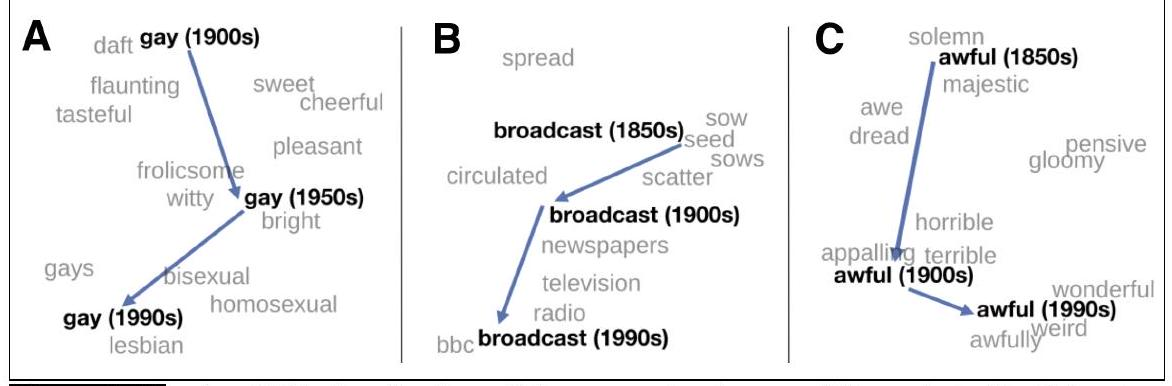
\includegraphics[max width=\textwidth, center]{2025_03_24_4f41283092a9d1f7a40eg-134}

Figure 6.17 A t-SNE visualization of the semantic change of 3 words in English using word2vec vectors. The modern sense of each word, and the grey context words, are computed from the most recent (modern) time-point embedding space. Earlier points are computed from earlier historical embedding spaces. The visualizations show the changes in the word gay from meanings related to "cheerful" or "frolicsome" to referring to homosexuality, the development of the modern "transmission" sense of broadcast from its original sense of sowing seeds, and the pejoration of the word awful as it shifted from meaning "full of awe" to meaning "terrible or appalling" (Hamilton et al., 2016b).

\subsection*{6.11 Bias and Embeddings}
In addition to their ability to learn word meaning from text, embeddings, alas, also reproduce the implicit biases and stereotypes that were latent in the text. As the prior section just showed, embeddings can roughly model relational similarity: 'queen' as the closest word to 'king' - 'man' + 'woman' implies the analogy man:woman::king:queen. But these same embedding analogies also exhibit gender stereotypes. For example Bolukbasi et al. (2016) find that the closest occupation to 'computer programmer' - 'man' + 'woman' in word2vec embeddings trained on news text is 'homemaker', and that the embeddings similarly suggest the analogy 'father' is to 'doctor' as 'mother' is to 'nurse'. This could result in what Crawford (2017) and Blodgett et al. (2020) call an allocational harm, when a system allocates resources (jobs or credit) unfairly to different groups. For example algorithms that use embeddings as part of a search for hiring potential programmers or doctors might thus incorrectly downweight documents with women's names.

It turns out that embeddings don't just reflect the statistics of their input, but also amplify bias; gendered terms become more gendered in embedding space than they were in the input text statistics (Zhao et al. 2017, Ethayarajh et al. 2019b, Jia et al. 2020), and biases are more exaggerated than in actual labor employment statistics (Garg et al., 2018).

Embeddings also encode the implicit associations that are a property of human reasoning. The Implicit Association Test (Greenwald et al., 1998) measures peo-\\
ple's associations between concepts (like 'flowers' or 'insects') and attributes (like 'pleasantness' and 'unpleasantness') by measuring differences in the latency with which they label words in the various categories. ${ }^{7}$ Using such methods, people in the United States have been shown to associate African-American names with unpleasant words (more than European-American names), male names more with mathematics and female names with the arts, and old people's names with unpleasant words (Greenwald et al. 1998, Nosek et al. 2002a, Nosek et al. 2002b). Caliskan et al. (2017) replicated all these findings of implicit associations using GloVe vectors and cosine similarity instead of human latencies. For example African-American names like 'Leroy' and 'Shaniqua' had a higher GloVe cosine with unpleasant words while European-American names ('Brad', 'Greg', 'Courtney') had a higher cosine with pleasant words. These problems with embeddings are an example of a representational harm (Crawford 2017, Blodgett et al. 2020), which is a harm caused by a system demeaning or even ignoring some social groups. Any embedding-aware algorithm that made use of word sentiment could thus exacerbate bias against African Americans.

Recent research focuses on ways to try to remove these kinds of biases, for example by developing a transformation of the embedding space that removes gender stereotypes but preserves definitional gender (Bolukbasi et al. 2016, Zhao et al. 2017) or changing the training procedure (Zhao et al., 2018b). However, although\\
debiasing these sorts of debiasing may reduce bias in embeddings, they do not eliminate it (Gonen and Goldberg, 2019), and this remains an open problem.

Historical embeddings are also being used to measure biases in the past. Garg et al. (2018) used embeddings from historical texts to measure the association between embeddings for occupations and embeddings for names of various ethnicities or genders (for example the relative cosine similarity of women's names versus men's to occupation words like 'librarian' or 'carpenter') across the 20th century. They found that the cosines correlate with the empirical historical percentages of women or ethnic groups in those occupations. Historical embeddings also replicated old surveys of ethnic stereotypes; the tendency of experimental participants in 1933 to associate adjectives like 'industrious' or 'superstitious' with, e.g., Chinese ethnicity, correlates with the cosine between Chinese last names and those adjectives using embeddings trained on 1930s text. They also were able to document historical gender biases, such as the fact that embeddings for adjectives related to competence ('smart', 'wise', 'thoughtful', 'resourceful') had a higher cosine with male than female words, and showed that this bias has been slowly decreasing since 1960. We return in later chapters to this question about the role of bias in natural language processing.

\subsection*{6.12 Evaluating Vector Models}
The most important evaluation metric for vector models is extrinsic evaluation on tasks, i.e., using vectors in an NLP task and seeing whether this improves performance over some other model.

\footnotetext{7 Roughly speaking, if humans associate 'flowers' with 'pleasantness' and 'insects' with 'unpleasantness', when they are instructed to push a green button for 'flowers' (daisy, iris, lilac) and 'pleasant words' (love, laughter, pleasure) and a red button for 'insects' (flea, spider, mosquito) and 'unpleasant words' (abuse, hatred, ugly) they are faster than in an incongruous condition where they push a red button for 'flowers' and 'unpleasant words' and a green button for 'insects' and 'pleasant words'.
}Nonetheless it is useful to have intrinsic evaluations. The most common metric is to test their performance on similarity, computing the correlation between an algorithm's word similarity scores and word similarity ratings assigned by humans. WordSim- 353 (Finkelstein et al., 2002) is a commonly used set of ratings from 0 to 10 for 353 noun pairs; for example (plane, car) had an average score of 5.77. SimLex-999 (Hill et al., 2015) is a more complex dataset that quantifies similarity (cup, mug) rather than relatedness (cup, coffee), and includes concrete and abstract adjective, noun and verb pairs. The TOEFL dataset is a set of 80 questions, each consisting of a target word with 4 additional word choices; the task is to choose which is the correct synonym, as in the example: Levied is closest in meaning to: imposed, believed, requested, correlated (Landauer and Dumais, 1997). All of these datasets present words without context.

Slightly more realistic are intrinsic similarity tasks that include context. The Stanford Contextual Word Similarity (SCWS) dataset (Huang et al., 2012) and the Word-in-Context (WiC) dataset (Pilehvar and Camacho-Collados, 2019) offer richer evaluation scenarios. SCWS gives human judgments on 2,003 pairs of words in their sentential context, while WiC gives target words in two sentential contexts that are either in the same or different senses; see Appendix G. The semantic textual similarity task (Agirre et al. 2012, Agirre et al. 2015) evaluates the performance of sentence-level similarity algorithms, consisting of a set of pairs of sentences, each pair with human-labeled similarity scores.

Another task used for evaluation is the analogy task, discussed on page 124, where the system has to solve problems of the form $a$ is to $b$ as $a^{*}$ is to $b^{*}$, given $a, b$, and $a^{*}$ and having to find $b^{*}$ (Turney and Littman, 2005). A number of sets of tuples have been created for this task (Mikolov et al. 2013a, Mikolov et al. 2013c, Gladkova et al. 2016), covering morphology (city:cities::child:children), lexicographic relations (leg:table::spout:teapot) and encyclopedia relations (Beijing:China::Dublin:Ireland), some drawing from the SemEval-2012 Task 2 dataset of 79 different relations (Jurgens et al., 2012).

All embedding algorithms suffer from inherent variability. For example because of randomness in the initialization and the random negative sampling, algorithms like word2vec may produce different results even from the same dataset, and individual documents in a collection may strongly impact the resulting embeddings (Tian et al. 2016, Hellrich and Hahn 2016, Antoniak and Mimno 2018). When embeddings are used to study word associations in particular corpora, therefore, it is best practice to train multiple embeddings with bootstrap sampling over documents and average the results (Antoniak and Mimno, 2018).

\subsection*{6.13 Summary}
\begin{itemize}
  \item In vector semantics, a word is modeled as a vector-a point in high-dimensional space, also called an embedding. In this chapter we focus on static embeddings, where each word is mapped to a fixed embedding.
  \item Vector semantic models fall into two classes: sparse and dense. In sparse models each dimension corresponds to a word in the vocabulary $V$ and cells are functions of co-occurrence counts. The term-document matrix has a row for each word (term) in the vocabulary and a column for each document. The word-context or term-term matrix has a row for each (target) word in\\
the vocabulary and a column for each context term in the vocabulary. Two sparse weightings are common: the tf-idf weighting which weights each cell by its term frequency and inverse document frequency, and PPMI (pointwise positive mutual information), which is most common for word-context matrices.
  \item Dense vector models have dimensionality 50-1000. Word2vec algorithms like skip-gram are a popular way to compute dense embeddings. Skip-gram trains a logistic regression classifier to compute the probability that two words are 'likely to occur nearby in text'. This probability is computed from the dot product between the embeddings for the two words.
  \item Skip-gram uses stochastic gradient descent to train the classifier, by learning embeddings that have a high dot product with embeddings of words that occur nearby and a low dot product with noise words.
  \item Other important embedding algorithms include GloVe, a method based on ratios of word co-occurrence probabilities.
  \item Whether using sparse or dense vectors, word and document similarities are computed by some function of the dot product between vectors. The cosine of two vectors-a normalized dot product-is the most popular such metric.
\end{itemize}

\section*{Bibliographical and Historical Notes}
The idea of vector semantics arose out of research in the 1950s in three distinct fields: linguistics, psychology, and computer science, each of which contributed a fundamental aspect of the model.

The idea that meaning is related to the distribution of words in context was widespread in linguistic theory of the 1950s, among distributionalists like Zellig Harris, Martin Joos, and J. R. Firth, and semioticians like Thomas Sebeok. As Joos (1950) put it,\\
the linguist's "meaning" of a morpheme. . . is by definition the set of conditional probabilities of its occurrence in context with all other morphemes.

The idea that the meaning of a word might be modeled as a point in a multidimensional semantic space came from psychologists like Charles E. Osgood, who had been studying how people responded to the meaning of words by assigning values along scales like happy/sad or hard/soft. Osgood et al. (1957) proposed that the meaning of a word in general could be modeled as a point in a multidimensional Euclidean space, and that the similarity of meaning between two words could be modeled as the distance between these points in the space.

A final intellectual source in the 1950s and early 1960s was the field then called

Some of the philosophical underpinning of the distributional way of thinking came from the late writings of the philosopher Wittgenstein, who was skeptical of the possibility of building a completely formal theory of meaning definitions for each word. Wittgenstein suggested instead that "the meaning of a word is its use in the language" (Wittgenstein, 1953, PI 43). That is, instead of using some logical language to define each word, or drawing on denotations or truth values, Wittgenstein's idea is that we should define a word by how it is used by people in speaking and understanding in their day-to-day interactions, thus prefiguring the movement toward embodied and experiential models in linguistics and NLP (Glenberg and Robertson 2000, Lake and Murphy 2021, Bisk et al. 2020, Bender and Koller 2020).

More distantly related is the idea of defining words by a vector of discrete features, which has roots at least as far back as Descartes and Leibniz (Wierzbicka 1992, Wierzbicka 1996). By the middle of the 20th century, beginning with the work of Hjelmslev (Hjelmslev, 1969) (originally 1943) and fleshed out in early models of generative grammar (Katz and Fodor, 1963), the idea arose of representing mean- ing with semantic features, symbols that represent some sort of primitive meaning. For example words like hen, rooster, or chick, have something in common (they all describe chickens) and something different (their age and sex), representable as:

\begin{verbatim}
hen +female, +chicken, +adult
rooster -female, +chicken, +adult
chick +chicken, -adult
\end{verbatim}

The dimensions used by vector models of meaning to define words, however, are only abstractly related to this idea of a small fixed number of hand-built dimensions. Nonetheless, there has been some attempt to show that certain dimensions of embedding models do contribute some specific compositional aspect of meaning like these early semantic features.

The use of dense vectors to model word meaning, and indeed the term embedding, grew out of the latent semantic indexing (LSI) model (Deerwester et al., 1988) recast as LSA (latent semantic analysis) (Deerwester et al., 1990). In LSA\\
singular value decomposition-SVD- is applied to a term-document matrix (each cell weighted by $\log$ frequency and normalized by entropy), and then the first 300 dimensions are used as the LSA embedding. Singular Value Decomposition (SVD) is a method for finding the most important dimensions of a data set, those dimensions along which the data varies the most. LSA was then quickly widely applied: as a cognitive model Landauer and Dumais (1997), and for tasks like spell checking (Jones and Martin, 1997), language modeling (Bellegarda 1997, Coccaro and Jurafsky 1998, Bellegarda 2000), morphology induction (Schone and Jurafsky 2000, Schone and Jurafsky 2001b), multiword expressions (MWEs) (Schone and Jurafsky, 2001a), and essay grading (Rehder et al., 1998). Related models were simultaneously developed and applied to word sense disambiguation by Schütze (1992b). LSA also led to the earliest use of embeddings to represent words in a probabilistic classifier, in the logistic regression document router of Schütze et al. (1995). The idea of SVD on the term-term matrix (rather than the term-document matrix) as a model of meaning for NLP was proposed soon after LSA by Schütze (1992b). Schütze applied the low-rank (97-dimensional) embeddings produced by SVD to the task of word sense disambiguation, analyzed the resulting semantic space, and also suggested possible techniques like dropping high-order dimensions. See Schütze (1997).

A number of alternative matrix models followed on from the early SVD work, including Probabilistic Latent Semantic Indexing (PLSI) (Hofmann, 1999), Latent

Dirichlet Allocation (LDA) (Blei et al., 2003), and Non-negative Matrix Factorization (NMF) (Lee and Seung, 1999).

The LSA community seems to have first used the word "embedding" in Landauer et al. (1997), in a variant of its mathematical meaning as a mapping from one space or mathematical structure to another. In LSA, the word embedding seems to have described the mapping from the space of sparse count vectors to the latent space of SVD dense vectors. Although the word thus originally meant the mapping from one space to another, it has metonymically shifted to mean the resulting dense vector in the latent space, and it is in this sense that we currently use the word.

By the next decade, Bengio et al. (2003) and Bengio et al. (2006) showed that neural language models could also be used to develop embeddings as part of the task of word prediction. Collobert and Weston (2007), Collobert and Weston (2008), and Collobert et al. (2011) then demonstrated that embeddings could be used to represent word meanings for a number of NLP tasks. Turian et al. (2010) compared the value of different kinds of embeddings for different NLP tasks. Mikolov et al. (2011) showed that recurrent neural nets could be used as language models. The idea of simplifying the hidden layer of these neural net language models to create the skipgram (and also CBOW) algorithms was proposed by Mikolov et al. (2013a). The negative sampling training algorithm was proposed in Mikolov et al. (2013b). There are numerous surveys of static embeddings and their parameterizations (Bullinaria and Levy 2007, Bullinaria and Levy 2012, Lapesa and Evert 2014, Kiela and Clark 2014, Levy et al. 2015).

See Manning et al. (2008) and Chapter 14 for a deeper understanding of the role of vectors in information retrieval, including how to compare queries with documents, more details on tf -idf, and issues of scaling to very large datasets. See Kim (2019) for a clear and comprehensive tutorial on word2vec. Cruse (2004) is a useful introductory linguistic text on lexical semantics.

\section*{Exercises}
\section*{7}
"[M]achines of this character can behave in a very complicated manner when the number of units is large."

Alan Turing (1948) "Intelligent Machines", page 6

Neural networks are a fundamental computational tool for language processing, and a very old one. They are called neural because their origins lie in the McCulloch-Pitts neuron (McCulloch and Pitts, 1943), a simplified model of the biological neuron as a kind of computing element that could be described in terms of propositional logic. But the modern use in language processing no longer draws on these early biological inspirations.

Instead, a modern neural network is a network of small computing units, each of which takes a vector of input values and produces a single output value. In this chapter we introduce the neural net applied to classification. The architecture we\\
feedforward\\
deep learning

\section*{Neural Networks}
 introduce is called a feedforward network because the computation proceeds iteratively from one layer of units to the next. The use of modern neural nets is often called deep learning, because modern networks are often deep (have many layers).Neural networks share much of the same mathematics as logistic regression. But neural networks are a more powerful classifier than logistic regression, and indeed a minimal neural network (technically one with a single 'hidden layer') can be shown to learn any function.

Neural net classifiers are different from logistic regression in another way. With logistic regression, we applied the regression classifier to many different tasks by developing many rich kinds of feature templates based on domain knowledge. When working with neural networks, it is more common to avoid most uses of rich handderived features, instead building neural networks that take raw words as inputs and learn to induce features as part of the process of learning to classify. We saw examples of this kind of representation learning for embeddings in Chapter 6. Nets that are very deep are particularly good at representation learning. For that reason deep neural nets are the right tool for tasks that offer sufficient data to learn features automatically.

In this chapter we'll introduce feedforward networks as classifiers, and also apply them to the simple task of language modeling: assigning probabilities to word sequences and predicting upcoming words. In subsequent chapters we'll introduce many other aspects of neural models, such as recurrent neural networks (Chapter 8), the Transformer (Chapter 9), and masked language modeling (Chapter 11).

\subsection*{7.1 Units}
The building block of a neural network is a single computational unit. A unit takes a set of real valued numbers as input, performs some computation on them, and produces an output.

At its heart, a neural unit is taking a weighted sum of its inputs, with one addi-\\
bias term tional term in the sum called a bias term. Given a set of inputs $x_{1} \ldots x_{n}$, a unit has a set of corresponding weights $w_{1} \ldots w_{n}$ and a bias $b$, so the weighted sum $z$ can be represented as:


\begin{equation*}
z=b+\sum_{i} w_{i} x_{i} \tag{7.1}
\end{equation*}


Often it's more convenient to express this weighted sum using vector notation; recall from linear algebra that a vector is, at heart, just a list or array of numbers. Thus we'll talk about $z$ in terms of a weight vector $w$, a scalar bias $b$, and an input vector $x$, and we'll replace the sum with the convenient dot product:


\begin{equation*}
z=\mathbf{w} \cdot \mathbf{x}+b \tag{7.2}
\end{equation*}


As defined in Eq. 7.2, $z$ is just a real valued number.\\
Finally, instead of using $z$, a linear function of $x$, as the output, neural units apply a non-linear function $f$ to $z$. We will refer to the output of this function as the activation value for the unit, $a$. Since we are just modeling a single unit, the activation for the node is in fact the final output of the network, which we'll generally call $y$. So the value $y$ is defined as:

$$
y=a=f(z)
$$

We'll discuss three popular non-linear functions $f$ below (the sigmoid, the tanh, and the rectified linear unit or ReLU) but it's pedagogically convenient to start with the sigmoid function since we saw it in Chapter 5:


\begin{equation*}
y=\sigma(z)=\frac{1}{1+e^{-z}} \tag{7.3}
\end{equation*}


The sigmoid (shown in Fig. 7.1) has a number of advantages; it maps the output into the range $(0,1)$, which is useful in squashing outliers toward 0 or 1 . And it's differentiable, which as we saw in Section 5.10 will be handy for learning.\\
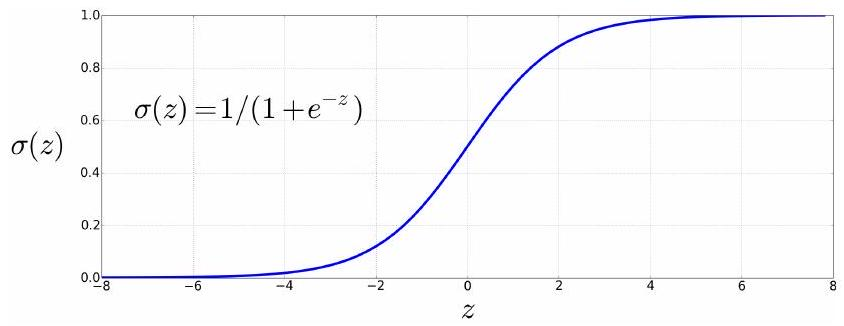
\includegraphics[max width=\textwidth, center]{2025_03_24_4f41283092a9d1f7a40eg-141}

Figure 7.1 The sigmoid function takes a real value and maps it to the range $(0,1)$. It is nearly linear around 0 but outlier values get squashed toward 0 or 1 .

Substituting Eq. 7.2 into Eq. 7.3 gives us the output of a neural unit:


\begin{equation*}
y=\sigma(\mathbf{w} \cdot \mathbf{x}+b)=\frac{1}{1+\exp (-(\mathbf{w} \cdot \mathbf{x}+b))} \tag{7.4}
\end{equation*}


Fig. 7.2 shows a final schematic of a basic neural unit. In this example the unit takes 3 input values $x_{1}, x_{2}$, and $x_{3}$, and computes a weighted sum, multiplying each value by a weight ( $w_{1}, w_{2}$, and $w_{3}$, respectively), adds them to a bias term $b$, and then passes the resulting sum through a sigmoid function to result in a number between 0 and 1.\\
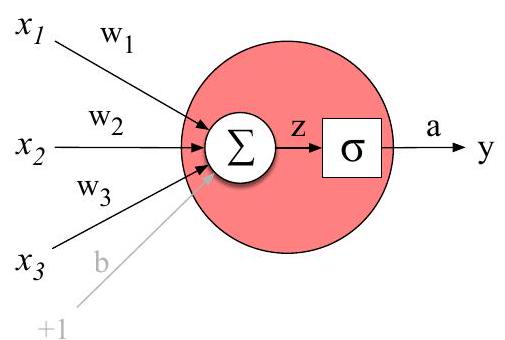
\includegraphics[max width=\textwidth, center]{2025_03_24_4f41283092a9d1f7a40eg-142}

Figure 7.2 A neural unit, taking 3 inputs $x_{1}, x_{2}$, and $x_{3}$ (and a bias $b$ that we represent as a weight for an input clamped at +1 ) and producing an output $y$. We include some convenient intermediate variables: the output of the summation, $z$, and the output of the sigmoid, $a$. In this case the output of the unit $y$ is the same as $a$, but in deeper networks we'll reserve $y$ to mean the final output of the entire network, leaving $a$ as the activation of an individual node.

Let's walk through an example just to get an intuition. Let's suppose we have a unit with the following weight vector and bias:

$$
\begin{aligned}
\mathbf{w} & =[0.2,0.3,0.9] \\
b & =0.5
\end{aligned}
$$

What would this unit do with the following input vector:

$$
\mathbf{x}=[0.5,0.6,0.1]
$$

The resulting output $y$ would be:\\
$y=\sigma(\mathbf{w} \cdot \mathbf{x}+b)=\frac{1}{1+e^{-(\mathbf{w} \cdot \mathbf{x}+b)}}=\frac{1}{1+e^{-(.5 * .2+.6 * .3+.1 * .9+.5)}}=\frac{1}{1+e^{-0.87}}=.70$\\
In practice, the sigmoid is not commonly used as an activation function. A function tanh is a variant of the sigmoid that ranges from -1 to +1 :


\begin{equation*}
y=\tanh (z)=\frac{e^{z}-e^{-z}}{e^{z}+e^{-z}} \tag{7.5}
\end{equation*}


The simplest activation function, and perhaps the most commonly used, is the rectified linear unit, also called the ReLU, shown in Fig. 7.3b. It's just the same as $z$ when $z$ is positive, and 0 otherwise:


\begin{equation*}
y=\operatorname{ReLU}(\mathrm{z})=\max (z, 0) \tag{7.6}
\end{equation*}


These activation functions have different properties that make them useful for different language applications or network architectures. For example, the tanh function has the nice properties of being smoothly differentiable and mapping outlier values toward the mean. The rectifier function, on the other hand, has nice properties that\\
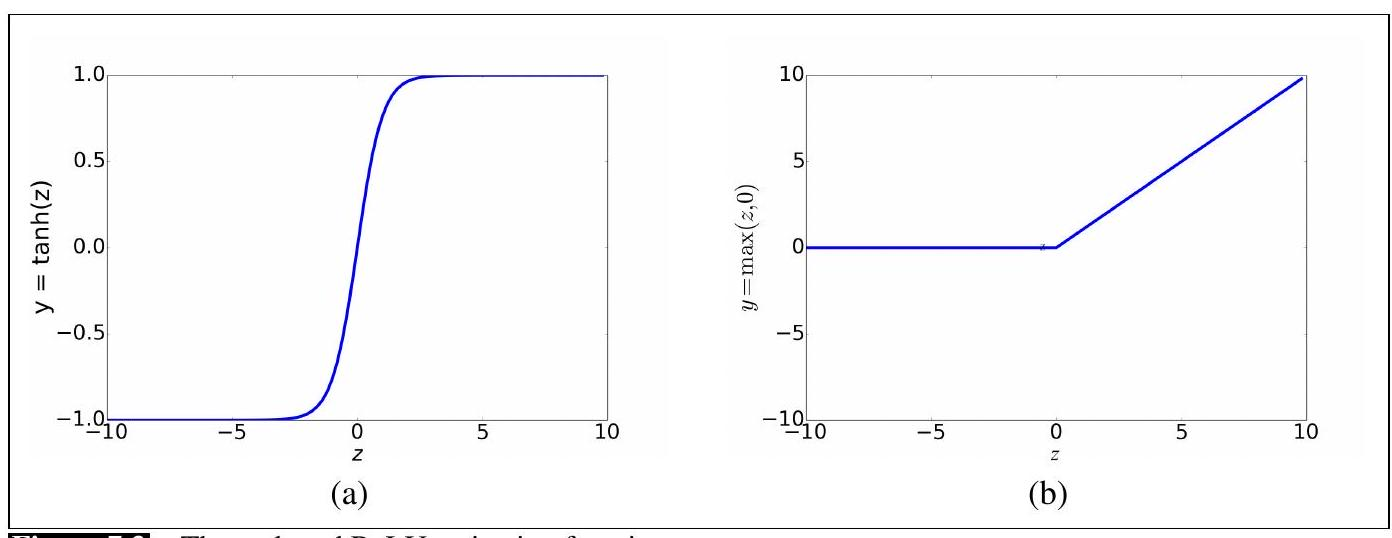
\includegraphics[max width=\textwidth, center]{2025_03_24_4f41283092a9d1f7a40eg-143}

Figure 7.3 The tanh and ReLU activation functions.\\
result from it being very close to linear. In the sigmoid or tanh functions, very high\\
values of $z$ result in values of $y$ that are saturated, i.e., extremely close to 1 , and have derivatives very close to 0 . Zero derivatives cause problems for learning, because as we'll see in Section 7.5, we'll train networks by propagating an error signal backwards, multiplying gradients (partial derivatives) from each layer of the network; gradients that are almost 0 cause the error signal to get smaller and smaller until it is too small to be used for training, a problem called the vanishing gradient problem. Rectifiers don't have this problem, since the derivative of ReLU for high values of $z$ is 1 rather than very close to 0 .

\subsection*{7.2 The XOR problem}
Early in the history of neural networks it was realized that the power of neural networks, as with the real neurons that inspired them, comes from combining these units into larger networks.

One of the most clever demonstrations of the need for multi-layer networks was the proof by Minsky and Papert (1969) that a single neural unit cannot compute some very simple functions of its input. Consider the task of computing elementary logical functions of two inputs, like AND, OR, and XOR. As a reminder, here are the truth tables for those functions:

\begin{center}
\begin{tabular}{cc|ccc|ccc|c}
\multicolumn{4}{c}{AND} & \multicolumn{3}{c}{OR} & \multicolumn{3}{c}{XOR} \\
\hline
$x 1$ & $x 2$ & $y$ & $x 1$ & $x 2$ & $y$ & $x 1$ & $x 2$ & $y$ &  \\
\hline
0 & 0 & 0 & 0 & 0 & 0 & 0 & 0 & 0 &  \\
0 & 1 & 0 & 0 & 1 & 1 & 0 & 1 & 1 &  \\
1 & 0 & 0 & 1 & 0 & 1 & 1 & 0 & 1 &  \\
1 & 1 & 1 & 1 & 1 & 1 & 1 & 1 & 0 &  \\
\end{tabular}
\end{center}

This example was first shown for the perceptron, which is a very simple neural unit that has a binary output and has a very simple step function as its non-linear activation function. The output $y$ of a perceptron is 0 or 1 , and is computed as follows (using the same weight $\mathbf{w}$, input $\mathbf{x}$, and bias $b$ as in Eq. 7.2):

\[
y= \begin{cases}0, & \text { if } \mathbf{w} \cdot \mathbf{x}+b \leq 0  \tag{7.7}\\ 1, & \text { if } \mathbf{w} \cdot \mathbf{x}+b>0\end{cases}
\]

It's very easy to build a perceptron that can compute the logical AND and OR functions of its binary inputs; Fig. 7.4 shows the necessary weights.\\
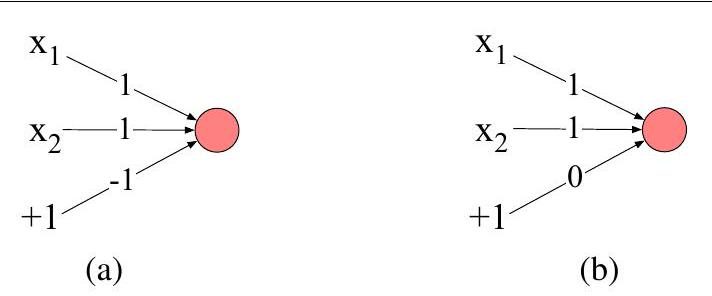
\includegraphics[max width=\textwidth, center]{2025_03_24_4f41283092a9d1f7a40eg-144}

Figure 7.4 The weights $w$ and bias $b$ for perceptrons for computing logical functions. The inputs are shown as $x_{1}$ and $x_{2}$ and the bias as a special node with value +1 which is multiplied with the bias weight $b$. (a) logical AND, with weights $w_{1}=1$ and $w_{2}=1$ and bias weight $b=-1$. (b) logical OR, with weights $w_{1}=1$ and $w_{2}=1$ and bias weight $b=0$. These weights/biases are just one from an infinite number of possible sets of weights and biases that would implement the functions.

It turns out, however, that it's not possible to build a perceptron to compute logical XOR! (It's worth spending a moment to give it a try!)

The intuition behind this important result relies on understanding that a perceptron is a linear classifier. For a two-dimensional input $x_{1}$ and $x_{2}$, the perceptron equation, $w_{1} x_{1}+w_{2} x_{2}+b=0$ is the equation of a line. (We can see this by putting it in the standard linear format: $x_{2}=\left(-w_{1} / w_{2}\right) x_{1}+\left(-b / w_{2}\right)$.) This line acts as a\\
decision boundary decision boundary in two-dimensional space in which the output 0 is assigned to all inputs lying on one side of the line, and the output 1 to all input points lying on the other side of the line. If we had more than 2 inputs, the decision boundary becomes a hyperplane instead of a line, but the idea is the same, separating the space into two categories.

Fig. 7.5 shows the possible logical inputs $(00,01,10$, and 11$)$ and the line drawn by one possible set of parameters for an AND and an OR classifier. Notice that there is simply no way to draw a line that separates the positive cases of XOR (01 and 10) from the negative cases (00 and 11). We say that XOR is not a linearly separable function. Of course we could draw a boundary with a curve, or some other function, but not a single line.

\subsection*{7.2.1 The solution: neural networks}
While the XOR function cannot be calculated by a single perceptron, it can be calculated by a layered network of perceptron units. Rather than see this with networks of simple perceptrons, however, let's see how to compute XOR using two layers of ReLU-based units following Goodfellow et al. (2016). Fig. 7.6 shows a figure with the input being processed by two layers of neural units. The middle layer (called h) has two units, and the output layer (called $y$ ) has one unit. A set of weights and biases are shown that allows the network to correctly compute the XOR function.

Let's walk through what happens with the input $\mathbf{x}=[0,0]$. If we multiply each input value by the appropriate weight, sum, and then add the bias $b$, we get the vector $[0,-1]$, and we then apply the rectified linear transformation to give the output of the h layer as [0, 0]. Now we once again multiply by the weights, sum, and add the bias ( 0 in this case) resulting in the value 0 . The reader should work through the computation of the remaining 3 possible input pairs to see that the resulting $y$ values are 1 for the inputs $[0,1]$ and $[1,0]$ and 0 for $[0,0]$ and $[1,1]$.\\
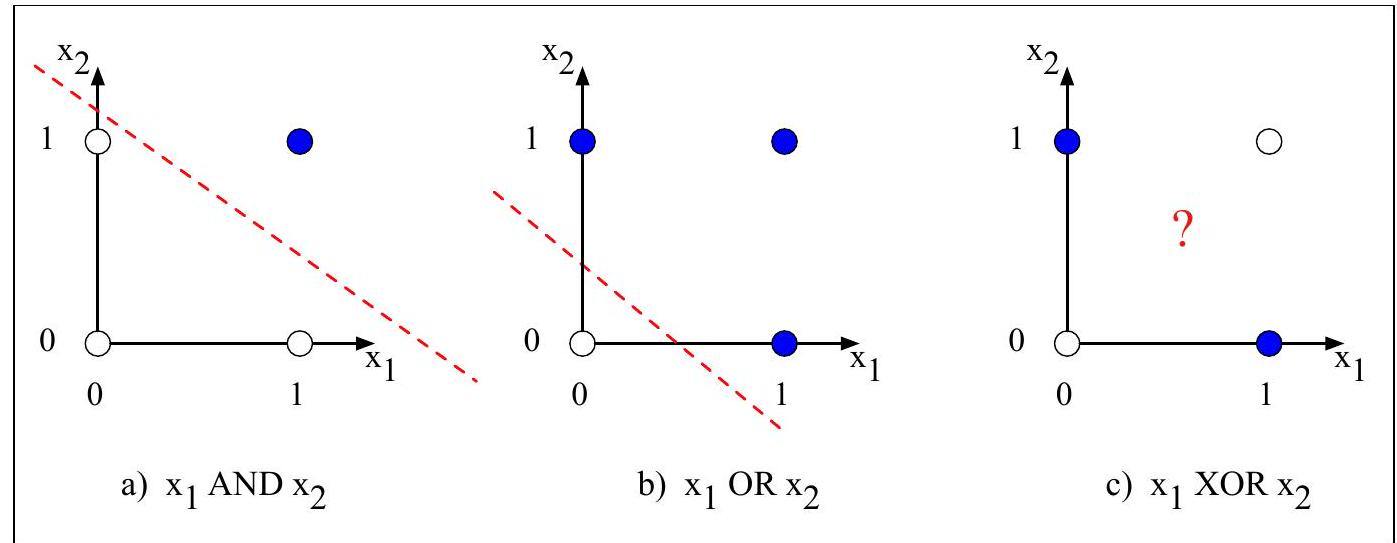
\includegraphics[max width=\textwidth, center]{2025_03_24_4f41283092a9d1f7a40eg-145}

Figure 7.5 The functions AND, OR, and XOR, represented with input $x_{1}$ on the x -axis and input $x_{2}$ on the $y$-axis. Filled circles represent perceptron outputs of 1 , and white circles perceptron outputs of 0 . There is no way to draw a line that correctly separates the two categories for XOR. Figure styled after Russell and Norvig (2002).\\
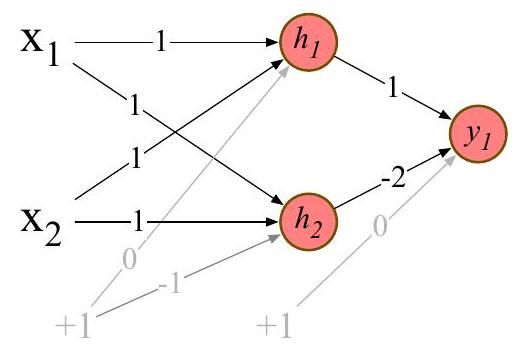
\includegraphics[max width=\textwidth, center]{2025_03_24_4f41283092a9d1f7a40eg-145(1)}

Figure 7.6 XOR solution after Goodfellow et al. (2016). There are three ReLU units, in two layers; we've called them $h_{1}, h_{2}$ ( $h$ for "hidden layer") and $y_{1}$. As before, the numbers on the arrows represent the weights $w$ for each unit, and we represent the bias $b$ as a weight on a unit clamped to +1 , with the bias weights/units in gray.

It's also instructive to look at the intermediate results, the outputs of the two hidden nodes $h_{1}$ and $h_{2}$. We showed in the previous paragraph that the $\mathbf{h}$ vector for the inputs $\mathbf{x}=[0,0]$ was $[0,0]$. Fig. 7.7b shows the values of the $\mathbf{h}$ layer for all 4 inputs. Notice that hidden representations of the two input points $x=[0,1]$ and $\mathbf{x}=[1,0]$ (the two cases with XOR output $=1$ ) are merged to the single point $\mathbf{h}=$ $[1,0]$. The merger makes it easy to linearly separate the positive and negative cases of XOR. In other words, we can view the hidden layer of the network as forming a representation of the input.

In this example we just stipulated the weights in Fig. 7.6. But for real examples the weights for neural networks are learned automatically using the error backpropagation algorithm to be introduced in Section 7.5. That means the hidden layers will learn to form useful representations. This intuition, that neural networks can automatically learn useful representations of the input, is one of their key advantages, and one that we will return to again and again in later chapters.\\
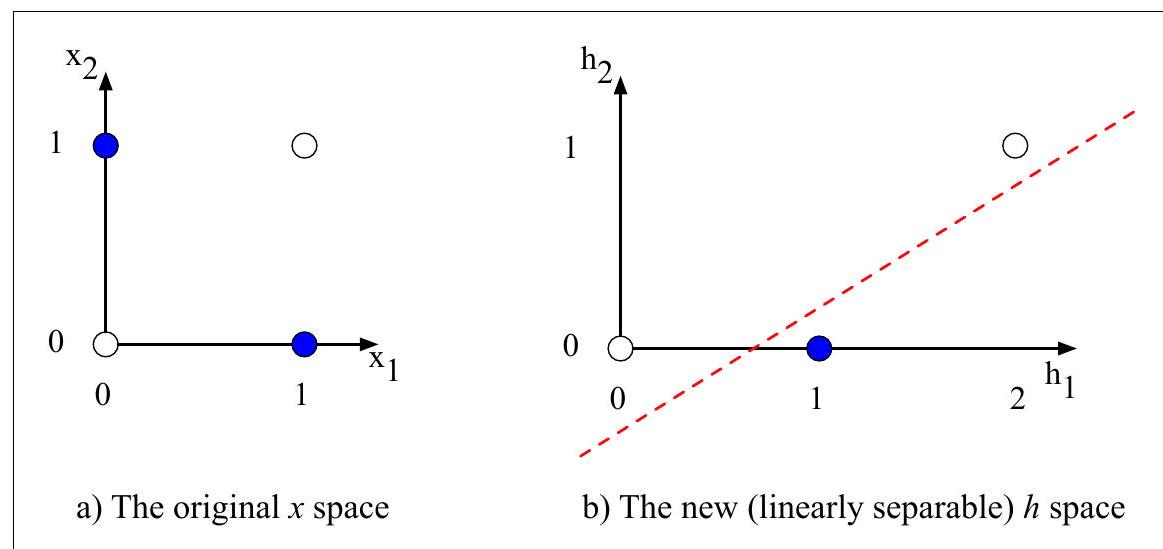
\includegraphics[max width=\textwidth, center]{2025_03_24_4f41283092a9d1f7a40eg-146}

Figure 7.7 The hidden layer forming a new representation of the input. (b) shows the representation of the hidden layer, $\mathbf{h}$, compared to the original input representation $\mathbf{x}$ in (a). Notice that the input point $[0,1]$ has been collapsed with the input point $[1,0]$, making it possible to linearly separate the positive and negative cases of XOR. After Goodfellow et al. (2016).

\subsection*{7.3 Feedforward Neural Networks}
feedforward network

Let's now walk through a slightly more formal presentation of the simplest kind of neural network, the feedforward network. A feedforward network is a multilayer network in which the units are connected with no cycles; the outputs from units in each layer are passed to units in the next higher layer, and no outputs are passed back to lower layers. (In Chapter 8 we'll introduce networks with cycles, called recurrent neural networks.)

For historical reasons multilayer networks, especially feedforward networks, are sometimes called multi-layer perceptrons (or MLPs); this is a technical misnomer, since the units in modern multilayer networks aren't perceptrons (perceptrons have a simple step-function as their activation function, but modern networks are made up of units with many kinds of non-linearities like ReLUs and sigmoids), but at some point the name stuck.

Simple feedforward networks have three kinds of nodes: input units, hidden units, and output units.

Fig. 7.8 shows a picture. The input layer $\mathbf{x}$ is a vector of simple scalar values just as we saw in Fig. 7.2.

The core of the neural network is the hidden layer $h$ formed of hidden units $\mathbf{h}_{i}$, each of which is a neural unit as described in Section 7.1, taking a weighted sum of its inputs and then applying a non-linearity. In the standard architecture, each layer is fully-connected, meaning that each unit in each layer takes as input the outputs from all the units in the previous layer, and there is a link between every pair of units from two adjacent layers. Thus each hidden unit sums over all the input units.

Recall that a single hidden unit has as parameters a weight vector and a bias. We represent the parameters for the entire hidden layer by combining the weight vector and bias for each unit $i$ into a single weight matrix $\mathbf{W}$ and a single bias vector $b$ for the whole layer (see Fig. 7.8). Each element $\mathbf{W}_{j i}$ of the weight matrix $\mathbf{W}$ represents the weight of the connection from the $i$ th input unit $x_{i}$ to the $j$ th hidden unit $h_{j}$.

The advantage of using a single matrix $\mathbf{W}$ for the weights of the entire layer is that now the hidden layer computation for a feedforward network can be done very\\
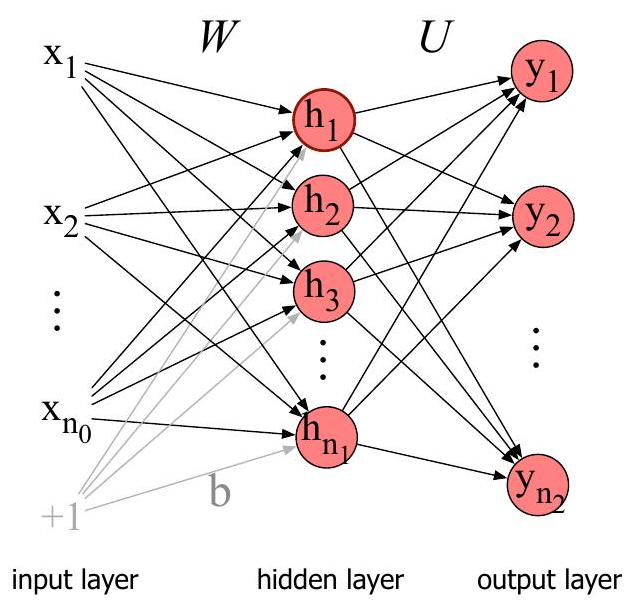
\includegraphics[max width=\textwidth, center]{2025_03_24_4f41283092a9d1f7a40eg-147}

Figure 7.8 A simple 2-layer feedforward network, with one hidden layer, one output layer, and one input layer (the input layer is usually not counted when enumerating layers).\\
efficiently with simple matrix operations. In fact, the computation only has three steps: multiplying the weight matrix by the input vector $\mathbf{x}$, adding the bias vector $\mathbf{b}$, and applying the activation function $g$ (such as the sigmoid, tanh, or ReLU activation function defined above).

The output of the hidden layer, the vector $\mathbf{h}$, is thus the following (for this example we'll use the sigmoid function $\sigma$ as our activation function):


\begin{equation*}
\mathbf{h}=\sigma(\mathbf{W} \mathbf{x}+\mathbf{b}) \tag{7.8}
\end{equation*}


Notice that we're applying the $\sigma$ function here to a vector, while in Eq. 7.3 it was applied to a scalar. We're thus allowing $\sigma(\cdot)$, and indeed any activation function $g(\cdot)$, to apply to a vector element-wise, so $g\left[z_{1}, z_{2}, z_{3}\right]=\left[g\left(z_{1}\right), g\left(z_{2}\right), g\left(z_{3}\right)\right]$.

Let's introduce some constants to represent the dimensionalities of these vectors and matrices. We'll refer to the input layer as layer 0 of the network, and have $n_{0}$ represent the number of inputs, so $\mathbf{x}$ is a vector of real numbers of dimension $n_{0}$, or more formally $\mathbf{x} \in \mathbb{R}^{n_{0}}$, a column vector of dimensionality $\left[n_{0}, 1\right]$. Let's call the hidden layer layer 1 and the output layer layer 2 . The hidden layer has dimensionality $n_{1}$, so $\mathbf{h} \in \mathbb{R}^{n_{1}}$ and also $\mathbf{b} \in \mathbb{R}^{n_{1}}$ (since each hidden unit can take a different bias value). And the weight matrix $\mathbf{W}$ has dimensionality $\mathbf{W} \in \mathbb{R}^{n_{1} \times n_{0}}$, i.e. $\left[n_{1}, n_{0}\right]$.

Take a moment to convince yourself that the matrix multiplication in Eq. 7.8 will compute the value of each $\mathbf{h}_{j}$ as $\sigma\left(\sum_{i=1}^{n_{0}} \mathbf{W}_{j i} \mathbf{x}_{i}+\mathbf{b}_{j}\right)$.

As we saw in Section 7.2, the resulting value $\mathbf{h}$ (for hidden but also for hypothesis) forms a representation of the input. The role of the output layer is to take this new representation $\mathbf{h}$ and compute a final output. This output could be a realvalued number, but in many cases the goal of the network is to make some sort of classification decision, and so we will focus on the case of classification.

If we are doing a binary task like sentiment classification, we might have a single output node, and its scalar value $y$ is the probability of positive versus negative sentiment. If we are doing multinomial classification, such as assigning a part-ofspeech tag, we might have one output node for each potential part-of-speech, whose output value is the probability of that part-of-speech, and the values of all the output nodes must sum to one. The output layer is thus a vector $\mathbf{y}$ that gives a probability distribution across the output nodes.

Let's see how this happens. Like the hidden layer, the output layer has a weight matrix (let's call it $\mathbf{U}$ ), but some models don't include a bias vector $\mathbf{b}$ in the output layer, so we'll simplify by eliminating the bias vector in this example. The weight matrix is multiplied by its input vector $(\mathbf{h})$ to produce the intermediate output $\mathbf{z}$ :

$$
\mathbf{z}=\mathbf{U h}
$$

There are $n_{2}$ output nodes, so $\mathbf{z} \in \mathbb{R}^{n_{2}}$, weight matrix $\mathbf{U}$ has dimensionality $\mathbf{U} \in$ $\mathbb{R}^{n_{2} \times n_{1}}$, and element $\mathbf{U}_{i j}$ is the weight from unit $j$ in the hidden layer to unit $i$ in the output layer.

However, $\mathbf{z}$ can't be the output of the classifier, since it's a vector of real-valued numbers, while what we need for classification is a vector of probabilities. There is a convenient function for normalizing a vector of real values, by which we mean converting it to a vector that encodes a probability distribution (all the numbers lie

\section*{softmax}
 between 0 and 1 and sum to 1 ): the softmax function that we saw on page 85 of Chapter 5. More generally for any vector $\mathbf{z}$ of dimensionality $d$, the softmax is defined as:
\begin{equation*}
\operatorname{softmax}\left(\mathbf{z}_{i}\right)=\frac{\exp \left(\mathbf{z}_{i}\right)}{\sum_{j=1}^{d} \exp \left(\mathbf{z}_{j}\right)} 1 \leq i \leq d \tag{7.9}
\end{equation*}


Thus for example given a vector


\begin{equation*}
\mathbf{z}=[0.6,1.1,-1.5,1.2,3.2,-1.1] \tag{7.10}
\end{equation*}


the softmax function will normalize it to a probability distribution (shown rounded):


\begin{equation*}
\operatorname{softmax}(\mathbf{z})=[0.055,0.090,0.0067,0.10,0.74,0.010] \tag{7.11}
\end{equation*}


You may recall that we used softmax to create a probability distribution from a vector of real-valued numbers (computed from summing weights times features) in the multinomial version of logistic regression in Chapter 5.

That means we can think of a neural network classifier with one hidden layer as building a vector $\mathbf{h}$ which is a hidden layer representation of the input, and then running standard multinomial logistic regression on the features that the network develops in $\mathbf{h}$. By contrast, in Chapter 5 the features were mainly designed by hand via feature templates. So a neural network is like multinomial logistic regression, but (a) with many layers, since a deep neural network is like layer after layer of logistic regression classifiers; (b) with those intermediate layers having many possible activation functions (tanh, ReLU, sigmoid) instead of just sigmoid (although we'll continue to use $\sigma$ for convenience to mean any activation function); (c) rather than forming the features by feature templates, the prior layers of the network induce the feature representations themselves.

Here are the final equations for a feedforward network with a single hidden layer, which takes an input vector $\mathbf{x}$, outputs a probability distribution $\mathbf{y}$, and is parameterized by weight matrices $\mathbf{W}$ and $\mathbf{U}$ and a bias vector $\mathbf{b}$ :


\begin{align*}
\mathbf{h} & =\boldsymbol{\sigma}(\mathbf{W} \mathbf{x}+\mathbf{b}) \\
\mathbf{z} & =\mathbf{U h} \\
\mathbf{y} & =\operatorname{softmax}(\mathbf{z}) \tag{7.12}
\end{align*}


And just to remember the shapes of all our variables, $\mathbf{x} \in \mathbb{R}^{n_{0}}, \mathbf{h} \in \mathbb{R}^{n_{1}}, \mathbf{b} \in \mathbb{R}^{n_{1}}$, $\mathbf{W} \in \mathbb{R}^{n_{1} \times n_{0}}, \mathbf{U} \in \mathbb{R}^{n_{2} \times n_{1}}$, and the output vector $\mathbf{y} \in \mathbb{R}^{n_{2}}$. We'll call this network a 2layer network (we traditionally don't count the input layer when numbering layers, but do count the output layer). So by this terminology logistic regression is a 1-layer network.

\subsection*{7.3.1 More details on feedforward networks}
Let's now set up some notation to make it easier to talk about deeper networks of depth more than 2 . We'll use superscripts in square brackets to mean layer numbers, starting at 0 for the input layer. So $\mathbf{W}^{[1]}$ will mean the weight matrix for the (first) hidden layer, and $\mathbf{b}^{[1]}$ will mean the bias vector for the (first) hidden layer. $n_{j}$ will mean the number of units at layer $j$. We'll use $g(\cdot)$ to stand for the activation function, which will tend to be ReLU or tanh for intermediate layers and softmax for output layers. We'll use $\mathbf{a}^{[i]}$ to mean the output from layer $i$, and $\mathbf{z}^{[i]}$ to mean the combination of previous layer output, weights and biases $\mathbf{W}^{[i]} \mathbf{a}^{[i-1]}+\mathbf{b}^{[i]}$. The 0th layer is for inputs, so we'll refer to the inputs $\mathbf{x}$ more generally as $\mathbf{a}^{[0]}$.

Thus we can re-represent our 2-layer net from Eq. 7.12 as follows:


\begin{align*}
\mathbf{z}^{[1]} & =\mathbf{W}^{[1]} \mathbf{a}^{[0]}+\mathbf{b}^{[1]} \\
\mathbf{a}^{[1]} & =g^{[1]}\left(\mathbf{z}^{[1]}\right) \\
\mathbf{z}^{[2]} & =\mathbf{W}^{[2]} \mathbf{a}^{[1]}+\mathbf{b}^{[2]} \\
\mathbf{a}^{[2]} & =g^{[2]}\left(\mathbf{z}^{[2]}\right) \\
\hat{\mathbf{y}} & =\mathbf{a}^{[2]} \tag{7.13}
\end{align*}


Note that with this notation, the equations for the computation done at each layer are the same. The algorithm for computing the forward step in an n-layer feedforward network, given the input vector $a^{[0]}$ is thus simply:

\begin{verbatim}
for $i$ in $1, \ldots, \mathrm{n}$
    $\mathbf{z}^{[i]}=\mathbf{W}^{[i]} \mathbf{a}^{[i-1]}+\mathbf{b}^{[i]}$
    $\mathbf{a}^{[i]}=g^{[i]}\left(\mathbf{z}^{[i]}\right)$
$\hat{\mathbf{y}}=\mathbf{a}^{[n]}$
\end{verbatim}

It's often useful to have a name for the final set of activations right before the final softmax. So however many layers we have, we'll generally call the unnormalized values in the final vector $\mathbf{z}^{[n]}$, the vector of scores right before the final softmax, the logits (see Eq. 5.7).

The need for non-linear activation functions One of the reasons we use nonlinear activation functions for each layer in a neural network is that if we did not, the resulting network is exactly equivalent to a single-layer network. Let's see why this is true. Imagine the first two layers of such a network of purely linear layers:

$$
\begin{aligned}
\mathbf{z}^{[1]} & =\mathbf{W}^{[1]} \mathbf{x}+\mathbf{b}^{[1]} \\
\mathbf{z}^{[2]} & =\mathbf{W}^{[2]} \mathbf{z}^{[1]}+\mathbf{b}^{[2]}
\end{aligned}
$$

We can rewrite the function that the network is computing as:


\begin{align*}
\mathbf{z}^{[2]} & =\mathbf{W}^{[2]} \mathbf{z}^{[1]}+\mathbf{b}^{[2]} \\
& =\mathbf{W}^{[2]}\left(\mathbf{W}^{[1]} \mathbf{x}+\mathbf{b}^{[1]}\right)+\mathbf{b}^{[2]} \\
& =\mathbf{W}^{[2]} \mathbf{W}^{[1]} \mathbf{x}+\mathbf{W}^{[2]} \mathbf{b}^{[1]}+\mathbf{b}^{[2]} \\
& =\mathbf{W}^{\prime} \mathbf{x}+\mathbf{b}^{\prime} \tag{7.14}
\end{align*}


This generalizes to any number of layers. So without non-linear activation functions, a multilayer network is just a notational variant of a single layer network with a different set of weights, and we lose all the representational power of multilayer networks.

Replacing the bias unit In describing networks, we will often use a slightly simplified notation that represents exactly the same function without referring to an explicit bias node $b$. Instead, we add a dummy node $\mathbf{a}_{0}$ to each layer whose value will always be 1 . Thus layer 0 , the input layer, will have a dummy node $\mathbf{a}_{0}^{[0]}=1$, layer 1 will have $\mathbf{a}_{0}^{[1]}=1$, and so on. This dummy node still has an associated weight, and that weight represents the bias value $b$. For example instead of an equation like


\begin{equation*}
\mathbf{h}=\sigma(\mathbf{W} \mathbf{x}+\mathbf{b}) \tag{7.15}
\end{equation*}


we'll use:


\begin{equation*}
\mathbf{h}=\sigma(\mathbf{W} \mathbf{x}) \tag{7.16}
\end{equation*}


But now instead of our vector $\mathbf{x}$ having $n_{0}$ values: $\mathbf{x}=\mathbf{x}_{1}, \ldots, \mathbf{x}_{n_{0}}$, it will have $n_{0}+$ 1 values, with a new 0 th dummy value $\mathbf{x}_{0}=1: \mathbf{x}=\mathbf{x}_{0}, \ldots, \mathbf{x}_{n_{0}}$. And instead of computing each $\mathbf{h}_{j}$ as follows:


\begin{equation*}
\mathbf{h}_{j}=\sigma\left(\sum_{i=1}^{n_{0}} \mathbf{W}_{j i} \mathbf{x}_{i}+\mathbf{b}_{j}\right) \tag{7.17}
\end{equation*}


we'll instead use:


\begin{equation*}
\mathbf{h}_{j}=\sigma\left(\sum_{i=0}^{n_{0}} \mathbf{W}_{j i} \mathbf{x}_{i}\right) \tag{7.18}
\end{equation*}


where the value $\mathbf{W}_{j 0}$ replaces what had been $\mathbf{b}_{j}$. Fig. 7.9 shows a visualization.\\
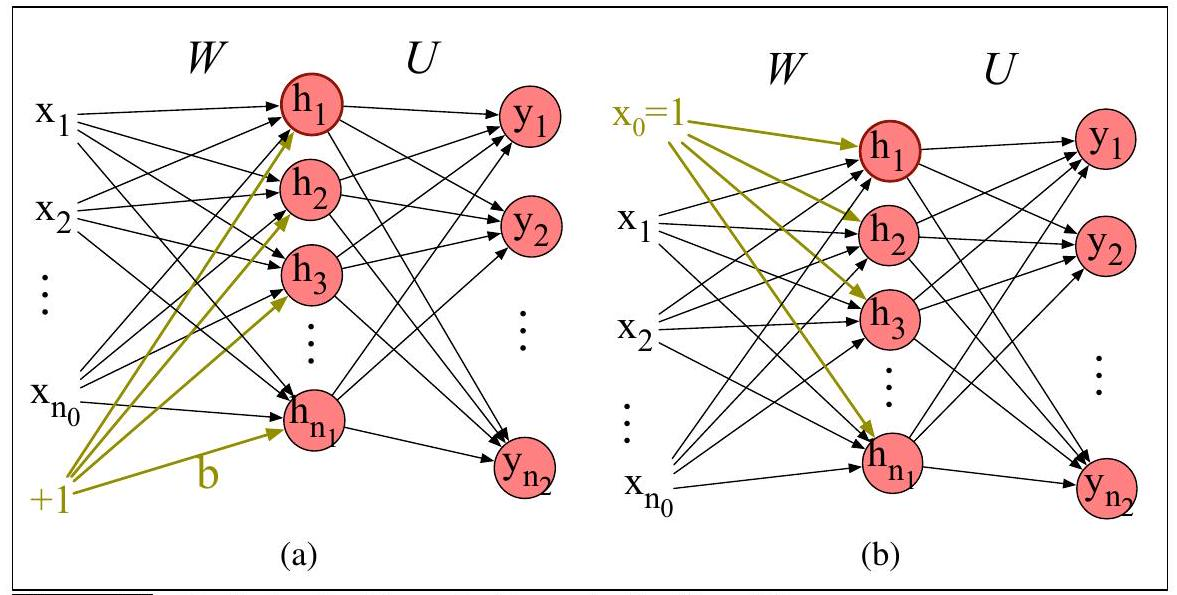
\includegraphics[max width=\textwidth, center]{2025_03_24_4f41283092a9d1f7a40eg-150}

Figure 7.9 Replacing the bias node (shown in a) with $x_{0}(\mathrm{~b})$.\\
We'll continue showing the bias as $b$ when we go over the learning algorithm in Section 7.5, but then we'll switch to this simplified notation without explicit bias terms for the rest of the book.

\subsection*{7.4 Feedforward networks for NLP: Classification}
Let's see how to apply feedforward networks to NLP tasks! In this section we'll look at classification tasks like sentiment analysis; in the next section we'll introduce neural language modeling.

Let's begin with a simple 2-layer sentiment classifier. You might imagine taking our logistic regression classifier from Chapter 5, which corresponds to a 1-layer network, and just adding a hidden layer. The input element $\mathbf{x}_{i}$ could be scalar features like those in Fig. 5.2, e.g., $\mathbf{x}_{1}=\operatorname{count}$ (words $\in \operatorname{doc}$ ), $\mathbf{x}_{2}=\operatorname{count}$ (positive lexicon words $\in \operatorname{doc}$ ), $\mathbf{x}_{3}=1$ if "no" $\in$ doc, and so on. And the output layer $\hat{\mathbf{y}}$ could have two nodes (one each for positive and negative), or 3 nodes (positive, negative, neutral), in which case $\hat{\mathbf{y}}_{1}$ would be the estimated probability of positive sentiment, $\hat{\mathbf{y}}_{2}$ the probability of negative and $\hat{\mathbf{y}}_{3}$ the probability of neutral. The resulting equations would be just what we saw above for a 2-layer network (as always, we'll continue to use the $\sigma$ to stand for any non-linearity, whether sigmoid, ReLU or other).


\begin{align*}
\mathbf{x} & =\left[\mathbf{x}_{1}, \mathbf{x}_{2}, \ldots \mathbf{x}_{N}\right] \quad \text { (each } \mathbf{x}_{i} \text { is a hand-designed feature) } \\
\mathbf{h} & =\sigma(\mathbf{W} \mathbf{x}+\mathbf{b}) \\
\mathbf{z} & =\mathbf{U h} \\
\hat{\mathbf{y}} & =\operatorname{softmax}(\mathbf{z}) \tag{7.19}
\end{align*}


Fig. 7.10 shows a sketch of this architecture. As we mentioned earlier, adding this hidden layer to our logistic regression classifier allows the network to represent the non-linear interactions between features. This alone might give us a better sentiment classifier.\\
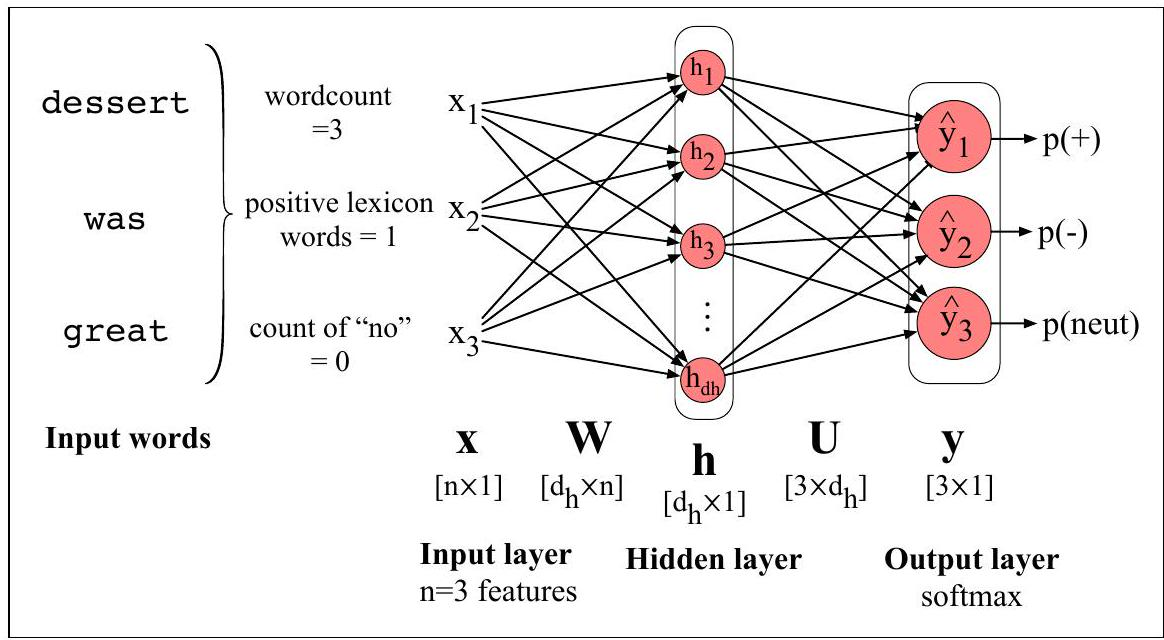
\includegraphics[max width=\textwidth, center]{2025_03_24_4f41283092a9d1f7a40eg-151}

Figure 7.10 Feedforward network sentiment analysis using traditional hand-built features of the input text.

Most applications of neural networks for NLP do something different, however. Instead of using hand-built human-engineered features as the input to our classifier, we draw on deep learning's ability to learn features from the data by representing words as embeddings, like the word2vec or GloVe embeddings we saw in Chapter 6. There are various ways to represent an input for classification. One simple baseline is to apply some sort of pooling function to the embeddings of all the words in the input. For example, for a text with $n$ input words/tokens $w_{1}, \ldots, w_{n}$, we can turn the $n$ embeddings $\mathbf{e}\left(w_{1}\right), \ldots, \mathbf{e}\left(w_{n}\right)$ (each of dimensionality $d$ ) into a single embedding also of dimensionality $d$ by just summing the embeddings, or by taking their mean (summing and then dividing by $n$ ):


\begin{equation*}
\mathbf{x}_{\text {mean }}=\frac{1}{n} \sum_{i=1}^{n} \mathbf{e}\left(w_{i}\right) \tag{7.20}
\end{equation*}


There are many other options, like taking the element-wise max. The element-wise max of a set of $n$ vectors is a new vector whose $k$ th element is the max of the $k$ th elements of all the $n$ vectors. Here are the equations for this classifier assuming mean pooling; the architecture is sketched in Fig. 7.11:


\begin{align*}
\mathbf{x} & =\operatorname{mean}\left(\mathbf{e}\left(w_{1}\right), \mathbf{e}\left(w_{2}\right), \ldots, \mathbf{e}\left(w_{n}\right)\right) \\
\mathbf{h} & =\sigma(\mathbf{W} \mathbf{x}+\mathbf{b}) \\
\mathbf{z} & =\mathbf{U h} \\
\hat{\mathbf{y}} & =\operatorname{softmax}(\mathbf{z}) \tag{7.21}
\end{align*}


\begin{center}
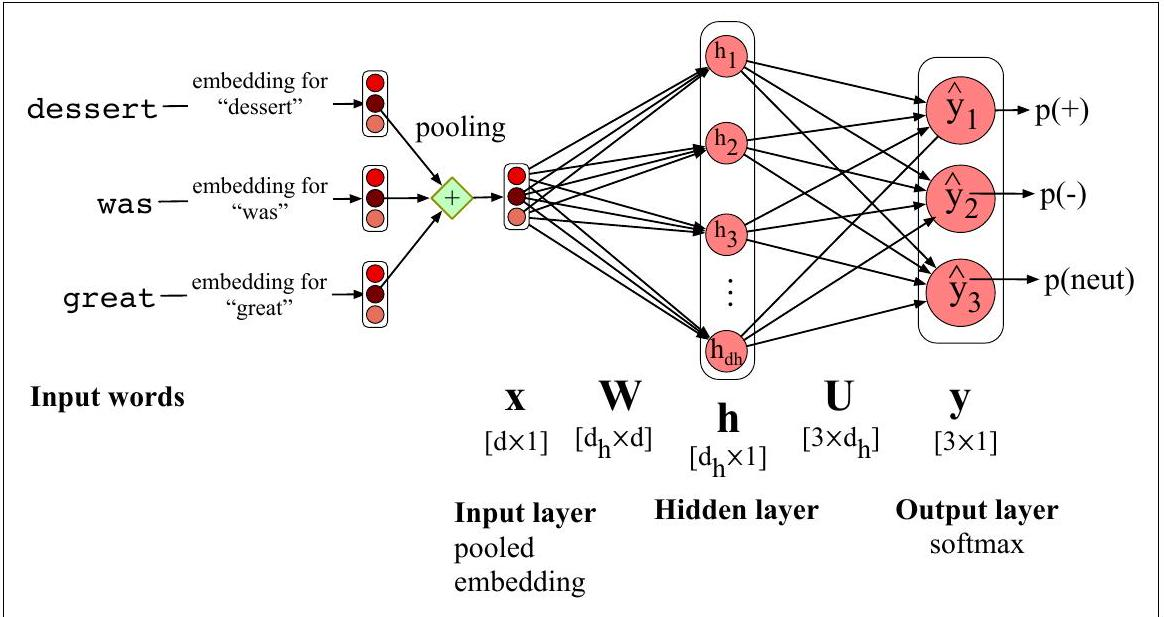
\includegraphics[max width=\textwidth]{2025_03_24_4f41283092a9d1f7a40eg-152}
\end{center}

Figure 7.11 Feedforward network sentiment analysis using a pooled embedding of the input words.

While Eq. 7.21 shows how to classify a single example $x$, in practice we want to efficiently classify an entire test set of $m$ examples. We do this by vectorizing the process, just as we saw with logistic regression; instead of using for-loops to go through each example, we'll use matrix multiplication to do the entire computation of an entire test set at once. First, we pack all the input feature vectors for each input $x$ into a single input matrix $\mathbf{X}$, with each row $i$ a row vector consisting of the pooled embedding for input example $x^{(i)}$ (i.e., the vector $\mathbf{x}^{(i)}$ ). If the dimensionality of our pooled input embedding is $d, \mathbf{X}$ will be a matrix of shape $[m \times d]$.

We will then need to slightly modify Eq. 7.21. $\mathbf{X}$ is of shape $[m \times d]$ and $\mathbf{W}$ is of shape $\left[d_{h} \times d\right]$, so we'll have to reorder how we multiply $\mathbf{X}$ and $\mathbf{W}$ and transpose $\mathbf{W}$ so they correctly multiply to yield a matrix $\mathbf{H}$ of shape $\left[m \times d_{h}\right] .{ }^{1}$ The bias vector $\mathbf{b}$ from Eq. 7.21 of shape $\left[1 \times d_{h}\right]$ will now have to be replicated into a matrix of shape $\left[m \times d_{h}\right]$. We'll need to similarly reorder the next step and transpose $\mathbf{U}$. Finally, our output matrix $\hat{\mathbf{Y}}$ will be of shape $[m \times 3]$ (or more generally $\left[m \times d_{o}\right.$ ], where $d_{o}$ is the number of output classes), with each row $i$ of our output matrix $\hat{\mathbf{Y}}$ consisting of the output vector $\hat{\mathbf{y}}^{(i)}$ ' Here are the final equations for computing the output class

\footnotetext{1 Note that we could have kept the original order of our products if we had instead made our input matrix $\mathbf{X}$ represent each input as a column vector instead of a row vector, making it of shape $[d \times m]$. But representing inputs as row vectors is convenient and common in neural network models.
}
distribution for an entire test set:\\
\$\$

\begin{align*}
\mathbf{H} & =\sigma\left(\mathbf{X} \mathbf{W}^{\top}+\mathbf{b}\right) \\
\mathbf{Z} & =\mathbf{H} \mathbf{U}^{\top} \\
\hat{\mathbf{Y}} & =\operatorname{softmax}(\mathbf{Z}) \tag{7.22}
\end{align*}

\$\$

The idea of using word2vec or GloVe embeddings as our input representationand more generally the idea of relying on another algorithm to have already learned

\section*{pretraining}
 an embedding representation for our input words-is called pretraining. Using pretrained embedding representations, whether simple static word embeddings like word2vec or the much more powerful contextual embeddings we'll introduce in Chapter 11, is one of the central ideas of deep learning. (It's also possible, however, to train the word embeddings as part of an NLP task; we'll talk about how to do this in Section 7.7 in the context of the neural language modeling task.)\subsection*{7.5 Training Neural Nets}
A feedforward neural net is an instance of supervised machine learning in which we know the correct output $y$ for each observation $x$. What the system produces, via Eq. 7.13, is $\hat{y}$, the system's estimate of the true $y$. The goal of the training procedure is to learn parameters $\mathbf{W}^{[i]}$ and $\mathbf{b}^{[i]}$ for each layer $i$ that make $\hat{y}$ for each training observation as close as possible to the true $y$.

In general, we do all this by drawing on the methods we introduced in Chapter 5 for logistic regression, so the reader should be comfortable with that chapter before proceeding.

First, we'll need a loss function that models the distance between the system output and the gold output, and it's common to use the loss function used for logistic regression, the cross-entropy loss.

Second, to find the parameters that minimize this loss function, we'll use the gradient descent optimization algorithm introduced in Chapter 5.

Third, gradient descent requires knowing the gradient of the loss function, the vector that contains the partial derivative of the loss function with respect to each of the parameters. In logistic regression, for each observation we could directly compute the derivative of the loss function with respect to an individual $w$ or $b$. But for neural networks, with millions of parameters in many layers, it's much harder to see how to compute the partial derivative of some weight in layer 1 when the loss is attached to some much later layer. How do we partial out the loss over all those intermediate layers? The answer is the algorithm called error backpropagation or backward differentiation.

\subsection*{7.5.1 Loss function}
The cross-entropy loss that is used in neural networks is the same one we saw for logistic regression. If the neural network is being used as a binary classifier, with the sigmoid at the final layer, the loss function is the same logistic regression loss we saw in Eq. 5.23:


\begin{equation*}
L_{C E}(\hat{y}, y)=-\log p(y \mid x)=-[y \log \hat{y}+(1-y) \log (1-\hat{y})] \tag{7.23}
\end{equation*}


If we are using the network to classify into 3 or more classes, the loss function is exactly the same as the loss for multinomial regression that we saw in Chapter 5 on\\
page 97. Let's briefly summarize the explanation here for convenience. First, when we have more than 2 classes we'll need to represent both $\mathbf{y}$ and $\hat{\mathbf{y}}$ as vectors. Let's assume we're doing hard classification, where only one class is the correct one. The true label $\mathbf{y}$ is then a vector with $K$ elements, each corresponding to a class, with $\mathbf{y}_{c}=1$ if the correct class is $c$, with all other elements of $\mathbf{y}$ being 0 . Recall that a vector like this, with one value equal to 1 and the rest 0 , is called a one-hot vector. And our classifier will produce an estimate vector with $K$ elements $\hat{\mathbf{y}}$, each element $\hat{\mathbf{y}}_{k}$ of which represents the estimated probability $p\left(\mathbf{y}_{k}=1 \mid \mathbf{x}\right)$.

The loss function for a single example $\mathbf{x}$ is the negative sum of the logs of the $K$ output classes, each weighted by their probability $y_{k}$ :


\begin{equation*}
L_{C E}(\hat{\mathbf{y}}, \mathbf{y})=-\sum_{k=1}^{K} \mathbf{y}_{k} \log \hat{\mathbf{y}}_{k} \tag{7.24}
\end{equation*}


We can simplify this equation further; let's first rewrite the equation using the function $\mathbb{1}\}$ which evaluates to 1 if the condition in the brackets is true and to 0 otherwise. This makes it more obvious that the terms in the sum in Eq. 7.24 will be 0 except for the term corresponding to the true class for which $\mathbf{y}_{k}=1$ :

$$
L_{C E}(\hat{\mathbf{y}}, \mathbf{y})=-\sum_{k=1}^{K} \mathbb{1}\left\{\mathbf{y}_{k}=1\right\} \log \hat{\mathbf{y}}_{k}
$$

In other words, the cross-entropy loss is simply the negative log of the output probability corresponding to the correct class, and we therefore also call this the negative log likelihood loss:


\begin{equation*}
L_{C E}(\hat{\mathbf{y}}, \mathbf{y})=-\log \hat{\mathbf{y}}_{c} \quad(\text { where } c \text { is the correct class) } \tag{7.25}
\end{equation*}


Plugging in the softmax formula from Eq. 7.9, and with $K$ the number of classes:


\begin{equation*}
L_{C E}(\hat{\mathbf{y}}, \mathbf{y})=-\log \frac{\exp \left(\mathbf{z}_{c}\right)}{\sum_{j=1}^{K} \exp \left(\mathbf{z}_{j}\right)} \quad \text { (where } c \text { is the correct class) } \tag{7.26}
\end{equation*}


\subsection*{7.5.2 Computing the Gradient}
How do we compute the gradient of this loss function? Computing the gradient requires the partial derivative of the loss function with respect to each parameter. For a network with one weight layer and sigmoid output (which is what logistic regression is), we could simply use the derivative of the loss that we used for logistic regression in Eq. 7.27 (and derived in Section 5.10):


\begin{align*}
\frac{\partial L_{C E}(\hat{\mathbf{y}}, \mathbf{y})}{\partial w_{j}} & =(\hat{y}-y) \mathbf{x}_{j} \\
& =(\sigma(\mathbf{w} \cdot \mathbf{x}+b)-y) \mathbf{x}_{j} \tag{7.27}
\end{align*}


Or for a network with one weight layer and softmax output (=multinomial logistic regression), we could use the derivative of the softmax loss from Eq. 5.48, shown for a particular weight $\mathbf{w}_{k}$ and input $\mathbf{x}_{i}$


\begin{align*}
\frac{\partial L_{\mathrm{CE}}(\hat{\mathbf{y}}, \mathbf{y})}{\partial \mathbf{w}_{k, i}} & =-\left(\mathbf{y}_{k}-\hat{\mathbf{y}}_{k}\right) \mathbf{x}_{i} \\
& =-\left(\mathbf{y}_{k}-p\left(\mathbf{y}_{k}=1 \mid \mathbf{x}\right)\right) \mathbf{x}_{i} \\
& =-\left(\mathbf{y}_{k}-\frac{\exp \left(\mathbf{w}_{\mathbf{k}} \cdot \mathbf{x}+b_{k}\right)}{\sum_{j=1}^{K} \exp \left(\mathbf{w}_{\mathbf{j}} \cdot \mathbf{x}+b_{j}\right)}\right) \mathbf{x}_{i} \tag{7.28}
\end{align*}


But these derivatives only give correct updates for one weight layer: the last one! For deep networks, computing the gradients for each weight is much more complex, since we are computing the derivative with respect to weight parameters that appear all the way back in the very early layers of the network, even though the loss is computed only at the very end of the network.

The solution to computing this gradient is an algorithm called error backprop-\\
error backpropagation agation or backprop (Rumelhart et al., 1986). While backprop was invented specially for neural networks, it turns out to be the same as a more general procedure called backward differentiation, which depends on the notion of computation graphs. Let's see how that works in the next subsection.

\subsection*{7.5.3 Computation Graphs}
A computation graph is a representation of the process of computing a mathematical expression, in which the computation is broken down into separate operations, each of which is modeled as a node in a graph.

Consider computing the function $L(a, b, c)=c(a+2 b)$. If we make each of the component addition and multiplication operations explicit, and add names ( $d$ and $e$ ) for the intermediate outputs, the resulting series of computations is:

$$
\begin{aligned}
d & =2 * b \\
e & =a+d \\
L & =c * e
\end{aligned}
$$

We can now represent this as a graph, with nodes for each operation, and directed edges showing the outputs from each operation as the inputs to the next, as in Fig. 7.12. The simplest use of computation graphs is to compute the value of the function with some given inputs. In the figure, we've assumed the inputs $a=3$, $b=1, c=-2$, and we've shown the result of the forward pass to compute the result $L(3,1,-2)=-10$. In the forward pass of a computation graph, we apply each operation left to right, passing the outputs of each computation as the input to the next node.\\
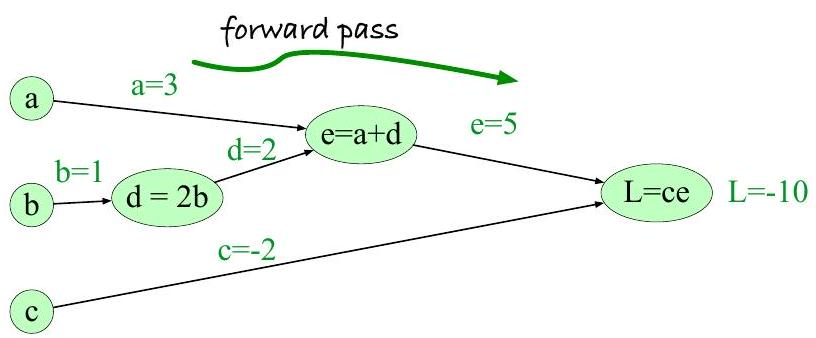
\includegraphics[max width=\textwidth, center]{2025_03_24_4f41283092a9d1f7a40eg-155}

Figure 7.12 Computation graph for the function $L(a, b, c)=c(a+2 b)$, with values for input nodes $a=3, b=1, c=-2$, showing the forward pass computation of $L$.

\subsection*{7.5.4 Backward differentiation on computation graphs}
The importance of the computation graph comes from the backward pass, which is used to compute the derivatives that we'll need for the weight update. In this example our goal is to compute the derivative of the output function $L$ with respect\\
to each of the input variables, i.e., $\frac{\partial L}{\partial a}, \frac{\partial L}{\partial b}$, and $\frac{\partial L}{\partial c}$. The derivative $\frac{\partial L}{\partial a}$ tells us how much a small change in $a$ affects $L$.\\
chain rule\\
Backwards differentiation makes use of the chain rule in calculus, so let's remind ourselves of that. Suppose we are computing the derivative of a composite function $f(x)=u(v(x))$. The derivative of $f(x)$ is the derivative of $u(x)$ with respect to $v(x)$ times the derivative of $v(x)$ with respect to $x$ :


\begin{equation*}
\frac{d f}{d x}=\frac{d u}{d v} \cdot \frac{d v}{d x} \tag{7.29}
\end{equation*}


The chain rule extends to more than two functions. If computing the derivative of a composite function $f(x)=u(v(w(x)))$, the derivative of $f(x)$ is:


\begin{equation*}
\frac{d f}{d x}=\frac{d u}{d v} \cdot \frac{d v}{d w} \cdot \frac{d w}{d x} \tag{7.30}
\end{equation*}


The intuition of backward differentiation is to pass gradients back from the final node to all the nodes in the graph. Fig. 7.13 shows part of the backward computation at one node $e$. Each node takes an upstream gradient that is passed in from its parent node to the right, and for each of its inputs computes a local gradient (the gradient of its output with respect to its input), and uses the chain rule to multiply these two to compute a downstream gradient to be passed on to the next earlier node.\\
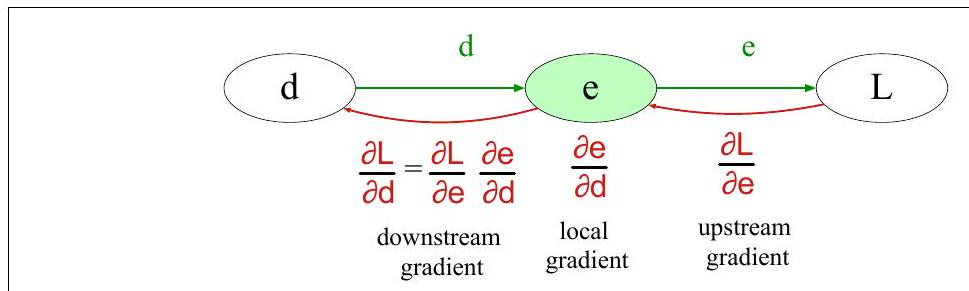
\includegraphics[max width=\textwidth, center]{2025_03_24_4f41283092a9d1f7a40eg-156}

Figure 7.13 Each node (like $e$ here) takes an upstream gradient, multiplies it by the local gradient (the gradient of its output with respect to its input), and uses the chain rule to compute a downstream gradient to be passed on to a prior node. A node may have multiple local gradients if it has multiple inputs.

Let's now compute the 3 derivatives we need. Since in the computation graph $L=c e$, we can directly compute the derivative $\frac{\partial L}{\partial c}$ :


\begin{equation*}
\frac{\partial L}{\partial c}=e \tag{7.31}
\end{equation*}


For the other two, we'll need to use the chain rule:


\begin{align*}
\frac{\partial L}{\partial a} & =\frac{\partial L}{\partial e} \frac{\partial e}{\partial a} \\
\frac{\partial L}{\partial b} & =\frac{\partial L}{\partial e} \frac{\partial e}{\partial d} \frac{\partial d}{\partial b} \tag{7.32}
\end{align*}


Eq. 7.32 and Eq. 7.31 thus require five intermediate derivatives: $\frac{\partial L}{\partial e}, \frac{\partial L}{\partial c}, \frac{\partial e}{\partial a}, \frac{\partial e}{\partial d}$, and $\frac{\partial d}{\partial b}$, which are as follows (making use of the fact that the derivative of a sum is the\\
sum of the derivatives):

$$
\begin{aligned}
L=c e: & \frac{\partial L}{\partial e}=c, \frac{\partial L}{\partial c}=e \\
e=a+d: & \frac{\partial e}{\partial a}=1, \frac{\partial e}{\partial d}=1 \\
d=2 b: & \frac{\partial d}{\partial b}=2
\end{aligned}
$$

In the backward pass, we compute each of these partials along each edge of the graph from right to left, using the chain rule just as we did above. Thus we begin by computing the downstream gradients from node $L$, which are $\frac{\partial L}{\partial e}$ and $\frac{\partial L}{\partial c}$. For node $e$, we then multiply this upstream gradient $\frac{\partial L}{\partial e}$ by the local gradient (the gradient of the output with respect to the input), $\frac{\partial e}{\partial d}$ to get the output we send back to node $\mathrm{d}: \frac{\partial L}{\partial d}$. And so on, until we have annotated the graph all the way to all the input variables. The forward pass conveniently already will have computed the values of the forward intermediate variables we need (like $d$ and $e$ ) to compute these derivatives. Fig. 7.14 shows the backward pass.\\
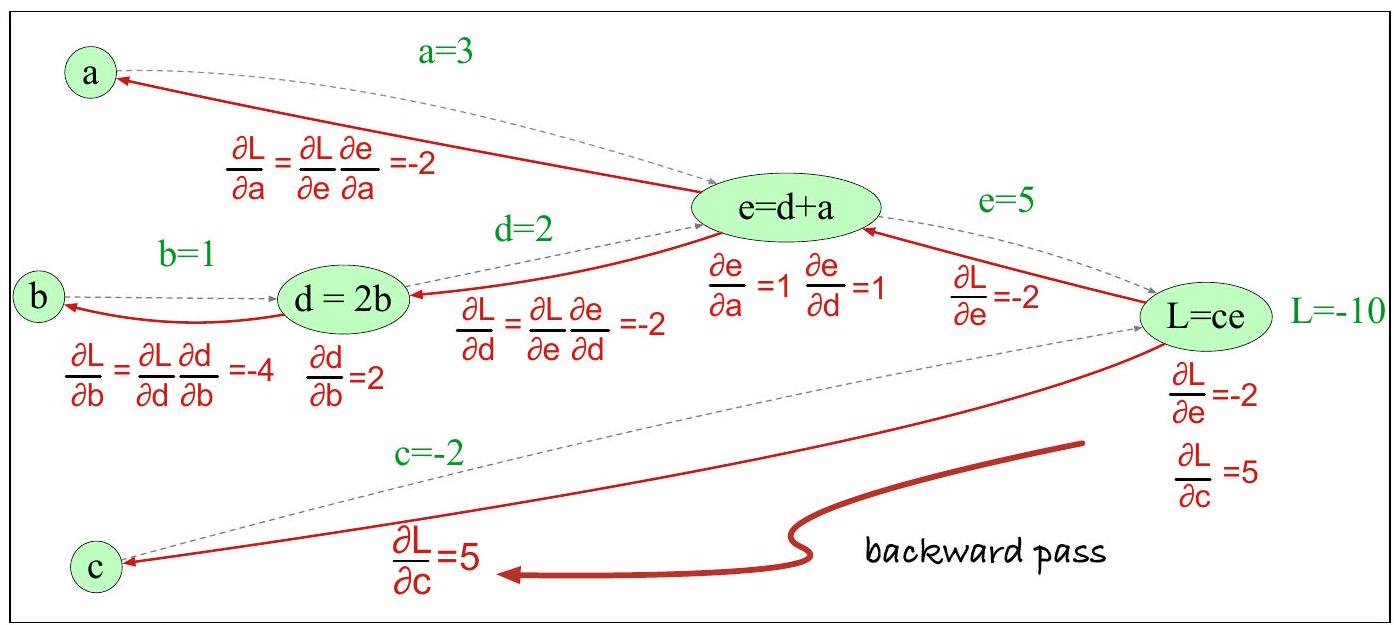
\includegraphics[max width=\textwidth, center]{2025_03_24_4f41283092a9d1f7a40eg-157}

Figure 7.14 Computation graph for the function $L(a, b, c)=c(a+2 b)$, showing the backward pass computation of $\frac{\partial L}{\partial a}, \frac{\partial L}{\partial b}$, and $\frac{\partial L}{\partial c}$.

\section*{Backward differentiation for a neural network}
Of course computation graphs for real neural networks are much more complex. Fig. 7.15 shows a sample computation graph for a 2-layer neural network with $n_{0}=$ $2, n_{1}=2$, and $n_{2}=1$, assuming binary classification and hence using a sigmoid output unit for simplicity. The function that the computation graph is computing is:


\begin{align*}
\mathbf{z}^{[1]} & =\mathbf{W}^{[1]} \mathbf{x}+\mathbf{b}^{[1]} \\
\mathbf{a}^{[1]} & =\operatorname{ReLU}\left(\mathbf{z}^{[1]}\right) \\
z^{[2]} & =\mathbf{W}^{[2]} \mathbf{a}^{[1]}+b^{[2]} \\
a^{[2]} & =\sigma\left(z^{[2]}\right) \\
\hat{y} & =a^{[2]} \tag{7.33}
\end{align*}


For the backward pass we'll also need to compute the loss $L$. The loss function for binary sigmoid output from Eq. 7.23 is


\begin{equation*}
L_{C E}(\hat{y}, y)=-[y \log \hat{y}+(1-y) \log (1-\hat{y})] \tag{7.34}
\end{equation*}


Our output $\hat{y}=a^{[2]}$, so we can rephrase this as


\begin{equation*}
L_{C E}\left(a^{[2]}, y\right)=-\left[y \log a^{[2]}+(1-y) \log \left(1-a^{[2]}\right)\right] \tag{7.35}
\end{equation*}


\begin{center}
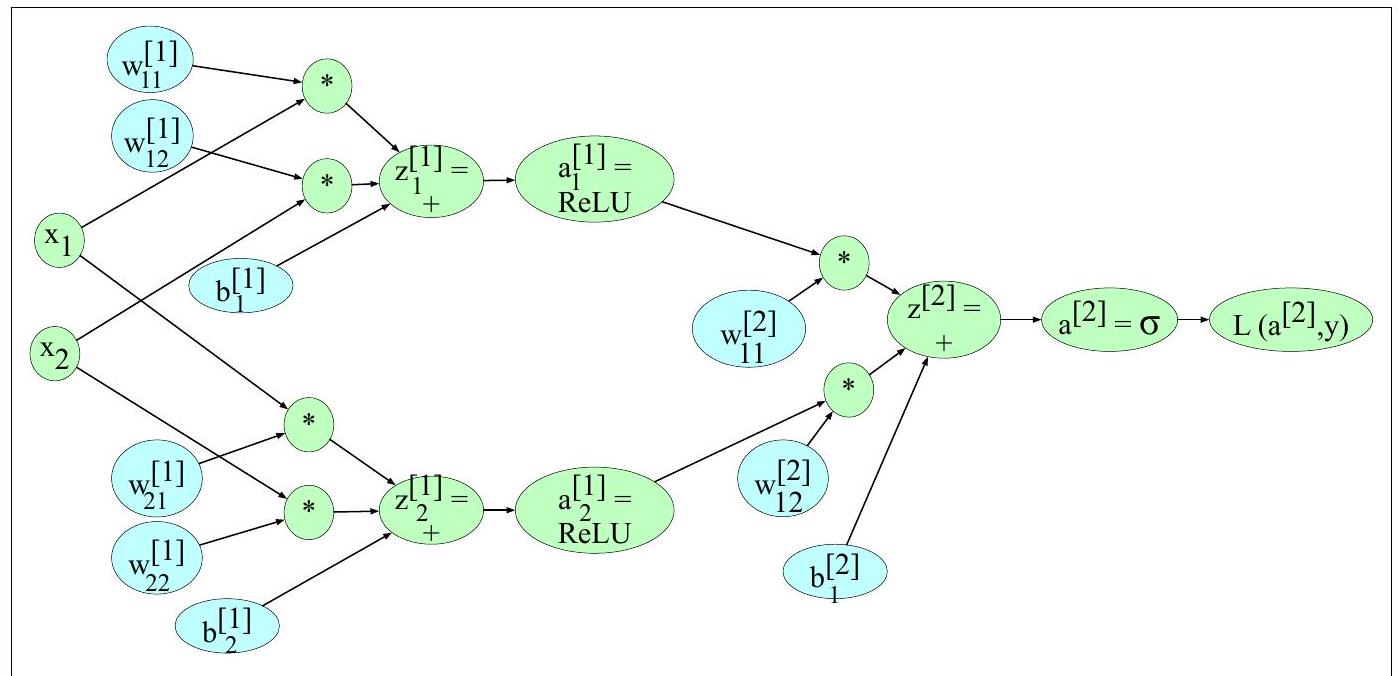
\includegraphics[max width=\textwidth]{2025_03_24_4f41283092a9d1f7a40eg-158}
\end{center}

Figure 7.15 Sample computation graph for a simple 2-layer neural net (= 1 hidden layer) with two input units and 2 hidden units. We've adjusted the notation a bit to avoid long equations in the nodes by just mentioning the function that is being computed, and the resulting variable name. Thus the * to the right of node $w_{11}^{[1]}$ means that $w_{11}^{[1]}$ is to be multiplied by $x_{1}$, and the node $z^{[1]}=+$ means that the value of $z^{[1]}$ is computed by summing the three nodes that feed into it (the two products, and the bias term $b_{i}^{[1]}$ ).

The weights that need updating (those for which we need to know the partial derivative of the loss function) are shown in teal. In order to do the backward pass, we'll need to know the derivatives of all the functions in the graph. We already saw in Section 5.10 the derivative of the sigmoid $\sigma$ :


\begin{equation*}
\frac{d \sigma(z)}{d z}=\sigma(z)(1-\sigma(z)) \tag{7.36}
\end{equation*}


We'll also need the derivatives of each of the other activation functions. The derivative of $\tanh$ is:


\begin{equation*}
\frac{d \tanh (z)}{d z}=1-\tanh ^{2}(z) \tag{7.37}
\end{equation*}


The derivative of the ReLU is ${ }^{2}$

\[
\frac{d \operatorname{ReLU}(z)}{d z}=\left\{\begin{array}{lll}
0 & \text { for } & z<0  \tag{7.38}\\
1 & \text { for } & z \geq 0
\end{array}\right.
\]

\footnotetext{2 The derivative is actually undefined at the point $z=0$, but by convention we treat it as 1 .
}We'll give the start of the computation, computing the derivative of the loss function $L$ with respect to $z$, or $\frac{\partial L}{\partial z}$ (and leaving the rest of the computation as an exercise for the reader). By the chain rule:


\begin{equation*}
\frac{\partial L}{\partial z}=\frac{\partial L}{\partial a^{[2]}} \frac{\partial a^{[2]}}{\partial z} \tag{7.39}
\end{equation*}


So let's first compute $\frac{\partial L}{\partial a^{[2]}}$, taking the derivative of Eq. 7.35, repeated here:


\begin{align*}
L_{C E}\left(a^{[2]}, y\right) & =-\left[y \log a^{[2]}+(1-y) \log \left(1-a^{[2]}\right)\right] \\
\frac{\partial L}{\partial a^{[2]}} & =-\left(\left(y \frac{\partial \log \left(a^{[2]}\right)}{\partial a^{[2]}}\right)+(1-y) \frac{\partial \log \left(1-a^{[2]}\right)}{\partial a^{[2]}}\right) \\
& =-\left(\left(y \frac{1}{a^{[2]}}\right)+(1-y) \frac{1}{1-a^{[2]}}(-1)\right) \\
& =-\left(\frac{y}{a^{[2]}}+\frac{y-1}{1-a^{[2]}}\right) \tag{7.40}
\end{align*}


Next, by the derivative of the sigmoid:

$$
\frac{\partial a^{[2]}}{\partial z}=a^{[2]}\left(1-a^{[2]}\right)
$$

Finally, we can use the chain rule:


\begin{align*}
\frac{\partial L}{\partial z} & =\frac{\partial L}{\partial a^{[2]}} \frac{\partial a^{[2]}}{\partial z} \\
& =-\left(\frac{y}{a^{[2]}}+\frac{y-1}{1-a^{[2]}}\right) a^{[2]}\left(1-a^{[2]}\right) \\
& =a^{[2]}-y \tag{7.41}
\end{align*}


Continuing the backward computation of the gradients (next by passing the gradients over $b_{1}^{[2]}$ and the two product nodes, and so on, back to all the teal nodes), is left as an exercise for the reader.

\subsection*{7.5.5 More details on learning}
Optimization in neural networks is a non-convex optimization problem, more complex than for logistic regression, and for that and other reasons there are many best practices for successful learning.

For logistic regression we can initialize gradient descent with all the weights and biases having the value 0 . In neural networks, by contrast, we need to initialize the weights with small random numbers. It's also helpful to normalize the input values to have 0 mean and unit variance.

Various forms of regularization are used to prevent overfitting. One of the most important is dropout: randomly dropping some units and their connections from the network during training (Hinton et al. 2012, Srivastava et al. 2014). At each iteration of training (whenever we update parameters, i.e. each mini-batch if we are using mini-batch gradient descent), we repeatedly choose a probability $p$ and for each unit we replace its output with zero with probability $p$ (and renormalize the rest of the outputs from that layer).

Tuning of hyperparameters is also important. The parameters of a neural network are the weights $\mathbf{W}$ and biases $\mathbf{b}$; those are learned by gradient descent. The hyperparameters are things that are chosen by the algorithm designer; optimal values are tuned on a devset rather than by gradient descent learning on the training set. Hyperparameters include the learning rate $\eta$, the mini-batch size, the model architecture (the number of layers, the number of hidden nodes per layer, the choice of activation functions), how to regularize, and so on. Gradient descent itself also has many architectural variants such as Adam (Kingma and Ba , 2015).

Finally, most modern neural networks are built using computation graph formalisms that make it easy and natural to do gradient computation and parallelization on vector-based GPUs (Graphic Processing Units). PyTorch (Paszke et al., 2017) and TensorFlow (Abadi et al., 2015) are two of the most popular. The interested reader should consult a neural network textbook for further details; some suggestions are at the end of the chapter.

\subsection*{7.6 Feedforward Neural Language Modeling}
As our second application of feedforward networks, let's consider language modeling: predicting upcoming words from prior words. Neural language modelingbased on the transformer architecture that we will see in Chapter 9-is the algorithm that underlies all of modern NLP. In this section and the next we'll introduce a simpler version of neural language models for feedforward networks, an algorithm first introduced by Bengio et al. (2003). The feedforward language model introduces many of the important concepts of neural language modeling, concepts we'll return to as we describe more powerful models in Chapter 8 and Chapter 9.

Neural language models have many advantages over the n -gram language models of Chapter 3. Compared to n-gram models, neural language models can handle much longer histories, can generalize better over contexts of similar words, and are more accurate at word-prediction. On the other hand, neural net language models are much more complex, are slower and need more energy to train, and are less interpretable than n-gram models, so for some smaller tasks an n-gram language model is still the right tool.

A feedforward neural language model (LM) is a feedforward network that takes as input at time $t$ a representation of some number of previous words $\left(w_{t-1}, w_{t-2}\right.$, etc.) and outputs a probability distribution over possible next words. Thus-like the n-gram LM-the feedforward neural LM approximates the probability of a word given the entire prior context $P\left(w_{t} \mid w_{1: t-1}\right)$ by approximating based on the $N-1$ previous words:


\begin{equation*}
P\left(w_{t} \mid w_{1}, \ldots, w_{t-1}\right) \approx P\left(w_{t} \mid w_{t-N+1}, \ldots, w_{t-1}\right) \tag{7.42}
\end{equation*}


In the following examples we'll use a 4-gram example, so we'll show a neural net to estimate the probability $P\left(w_{t}=i \mid w_{t-3}, w_{t-2}, w_{t-1}\right)$.

Neural language models represent words in this prior context by their embeddings, rather than just by their word identity as used in n-gram language models. Using embeddings allows neural language models to generalize better to unseen data. For example, suppose we've seen this sentence in training:

I have to make sure that the cat gets fed.\\
but have never seen the words "gets fed" after the word "dog". Our test set has the prefix "I forgot to make sure that the dog gets". What's the next word? An n-gram language model will predict "fed" after "that the cat gets", but not after "that the dog gets". But a neural LM, knowing that "cat" and "dog" have similar embeddings, will be able to generalize from the "cat" context to assign a high enough probability to "fed" even after seeing "dog".

\subsection*{7.6.1 Forward inference in the neural language model}
forward inference

Let's walk through forward inference or decoding for neural language models. Forward inference is the task, given an input, of running a forward pass on the network to produce a probability distribution over possible outputs, in this case next words.

We first represent each of the $N$ previous words as a one-hot vector of length $|V|$, i.e., with one dimension for each word in the vocabulary. A one-hot vector is a vector that has one element equal to 1 -in the dimension corresponding to that word's index in the vocabulary- while all the other elements are set to zero. Thus in a one-hot representation for the word "toothpaste", supposing it is $V_{5}$, i.e., index 5 in the vocabulary, $x_{5}=1$, and $x_{i}=0 \forall i \neq 5$, as shown here:

$$
\left[\begin{array}{rrrrrrrrrrrr}
0 & 0 & 0 & 0 & 1 & 0 & 0 & \ldots & 0 & 0 & 0 & 0
\end{array}\right]
$$

The feedforward neural language model (sketched in Fig. 7.17) has a moving window that can see N words into the past. We'll let N equal 3 , so the 3 words $w_{t-1}, w_{t-2}$, and $w_{t-3}$ are each represented as a one-hot vector. We then multiply these one-hot vectors by the embedding matrix $\mathbf{E}$. The embedding weight matrix $\mathbf{E}$ has a column for each word, each a column vector of $d$ dimensions, and hence has dimensionality $d \times|V|$. Multiplying by a one-hot vector that has only one non-zero element $x_{i}=1$ simply selects out the relevant column vector for word $i$, resulting in the embedding for word $i$, as shown in Fig. 7.16.\\
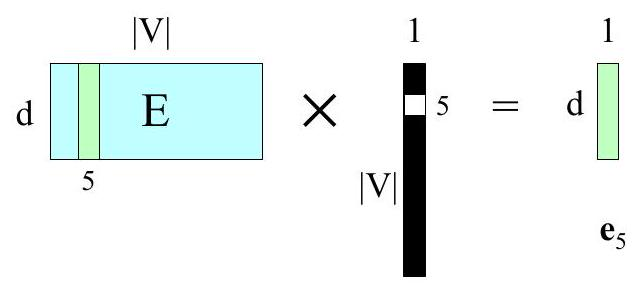
\includegraphics[max width=\textwidth, center]{2025_03_24_4f41283092a9d1f7a40eg-161}

Figure 7.16 Selecting the embedding vector for word $V_{5}$ by multiplying the embedding matrix $\mathbf{E}$ with a one-hot vector with a 1 in index 5 .

The 3 resulting embedding vectors are concatenated to produce $\mathbf{e}$, the embedding layer. This is followed by a hidden layer and an output layer whose softmax produces a probability distribution over words. For example $y_{42}$, the value of output node 42, is the probability of the next word $w_{t}$ being $V_{42}$, the vocabulary word with index 42 (which is the word 'fish' in our example).

Here's the algorithm in detail for our mini example:

\begin{enumerate}
  \item Select three embeddings from E: Given the three previous words, we look up their indices, create 3 one-hot vectors, and then multiply each by the embedding matrix $\mathbf{E}$. Consider $w_{t-3}$. The one-hot vector for 'for' (index 35) is multiplied by the embedding matrix $\mathbf{E}$, to give the first part of the first hidden\\
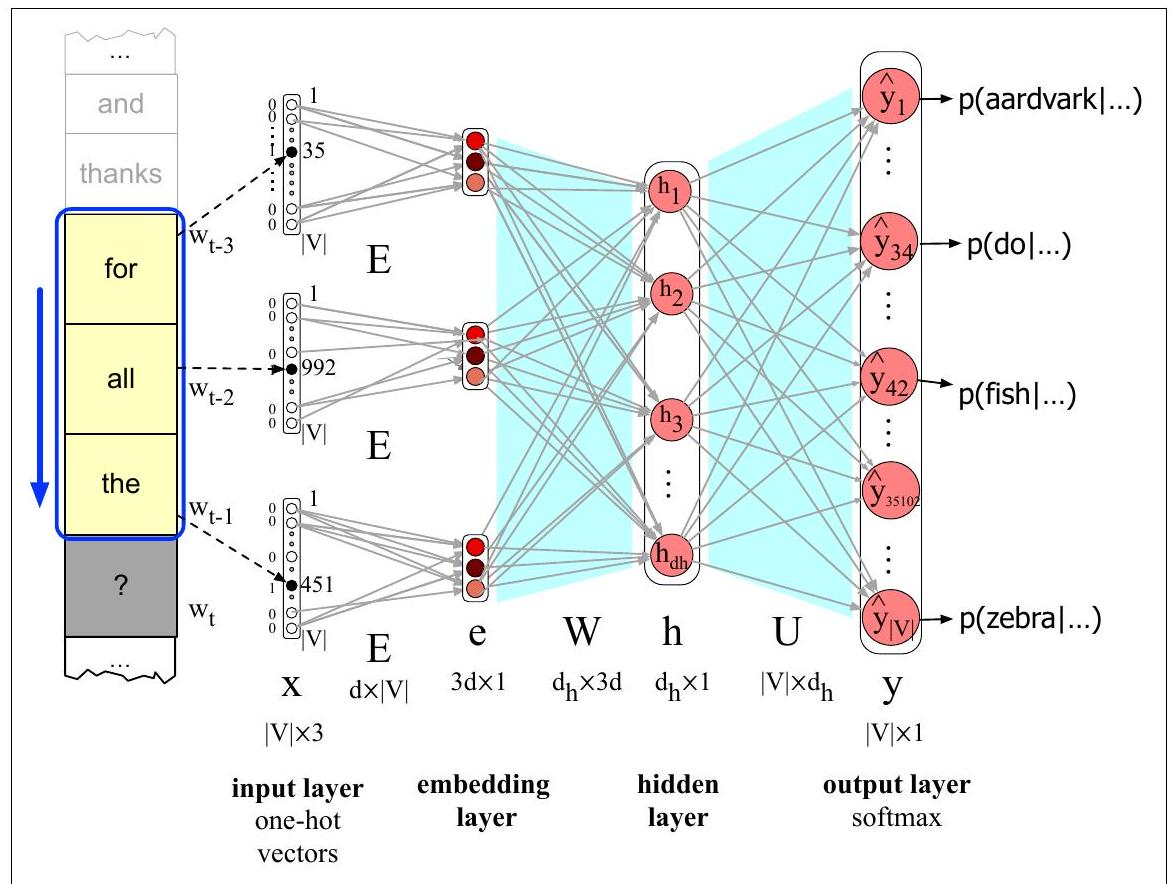
\includegraphics[max width=\textwidth, center]{2025_03_24_4f41283092a9d1f7a40eg-162}
\end{enumerate}

Figure 7.17 Forward inference in a feedforward neural language model. At each timestep $t$ the network computes a $d$-dimensional embedding for each context word (by multiplying a one-hot vector by the embedding matrix $\mathbf{E}$ ), and concatenates the 3 resulting embeddings to get the embedding layer $\mathbf{e}$. The embedding vector $\mathbf{e}$ is multiplied by a weight matrix $\mathbf{W}$ and then an activation function is applied element-wise to produce the hidden layer $\mathbf{h}$, which is then multiplied by another weight matrix $\mathbf{U}$. Finally, a softmax output layer predicts at each node $i$ the probability that the next word $w_{t}$ will be vocabulary word $V_{i}$.\\
embedding layer\\
layer, the embedding layer. Since each column of the input matrix $\mathbf{E}$ is an embedding for a word, and the input is a one-hot column vector $\mathbf{x}_{\boldsymbol{i}}$ for word $V_{i}$, the embedding layer for input $w$ will be $\mathbf{E} \mathbf{x}_{\mathbf{i}}=\mathbf{e}_{\mathbf{i}}$, the embedding for word $i$. We now concatenate the three embeddings for the three context words to produce the embedding layer $\mathbf{e}$.\\
2. Multiply by W: We multiply by $W$ (and add $b$ ) and pass through the ReLU (or other) activation function to get the hidden layer $h$.\\
3. Multiply by $\mathbf{U}: h$ is now multiplied by $U$\\
4. Apply softmax: After the softmax, each node $i$ in the output layer estimates the probability $P\left(w_{t}=i \mid w_{t-1}, w_{t-2}, w_{t-3}\right)$\\
In summary, the equations for a neural language model with a window size of 3 , given one-hot input vectors for each input context word, are:


\begin{align*}
\mathbf{e} & =\left[\mathbf{E} \mathbf{x}_{\mathbf{t}-\mathbf{3}} ; \mathbf{E} \mathbf{x}_{\mathbf{t}-\mathbf{2}} ; \mathbf{E} \mathbf{x}_{\mathbf{t}-\mathbf{1}}\right] \\
\mathbf{h} & =\sigma(\mathbf{W e}+\mathbf{b}) \\
\mathbf{z} & =\mathbf{U h} \\
\hat{\mathbf{y}} & =\operatorname{softmax}(\mathbf{z}) \tag{7.43}
\end{align*}


Note that we formed the embedding layer e by concatenating the 3 embeddings for the three context vectors; we'll often use semicolons to mean concatenation of vectors.

\subsection*{7.7 Training the neural language model}
The high-level intuition of training neural language models, whether the simple feedforward language models we describe here or the more powerful transformer\\
language models of Chapter 9, is the idea of self-training or self-supervision that we saw in Chapter 6 for learning word representations. In self-training for language modeling, we take a corpus of text as training material and at each time step $t$ ask the model to predict the next word. At first it will do poorly at this task, but since in each case we know the correct answer (it's the next word in the corpus!) we can easily train it to be better at predicting the correct next word. We call such a model self-supervised because we don't have to add any special gold labels to the data; the natural sequence of words is its own supervision! We simply train the model to minimize the error in predicting the true next word in the training sequence.

In practice, training the model means setting the parameters $\theta=\mathbf{E}, \mathbf{W}, \mathbf{U}, \mathbf{b}$. For freeze some tasks, it's ok to freeze the embedding layer $\mathbf{E}$ with initial word2vec values. Freezing means we use word2vec or some other pretraining algorithm to compute the initial embedding matrix $\mathbf{E}$, and then hold it constant while we only modify $\mathbf{W}$, $\mathbf{U}$, and $\mathbf{b}$, i.e., we don't update $\mathbf{E}$ during language model training. However, often we'd like to learn the embeddings simultaneously with training the network. This is useful when the task the network is designed for (like sentiment classification, translation, or parsing) places strong constraints on what makes a good representation for words.

Let's see how to train the entire model including E, i.e. to set all the parameters $\theta=\mathbf{E}, \mathbf{W}, \mathbf{U}, \mathbf{b}$. We'll do this via gradient descent (Fig. 5.6), using error backpropagation on the computation graph to compute the gradient. Training thus not only sets the weights $\mathbf{W}$ and $\mathbf{U}$ of the network, but also as we're predicting upcoming words, we're learning the embeddings $\mathbf{E}$ for each word that best predict upcoming words.

Fig. 7.18 shows the set up for a window size of $\mathrm{N}=3$ context words. The input $\mathbf{x}$ consists of 3 one-hot vectors, fully connected to the embedding layer via 3 instantiations of the embedding matrix $E$. We don't want to learn separate weight matrices for mapping each of the 3 previous words to the projection layer. We want one single embedding dictionary $E$ that's shared among these three. That's because over time, many different words will appear as $w_{t-2}$ or $w_{t-1}$, and we'd like to just represent each word with one vector, whichever context position it appears in. Recall that the embedding weight matrix $E$ has a column for each word, each a column vector of $d$ dimensions, and hence has dimensionality $d \times|V|$.

Generally training proceeds by taking as input a very long text, concatenating all the sentences, starting with random weights, and then iteratively moving through the text predicting each word $w_{t}$. At each word $w_{t}$, we use the cross-entropy (negative $\log$ likelihood) loss. Recall that the general form for this (repeated from Eq. 7.25) is:


\begin{equation*}
L_{C E}(\hat{y}, y)=-\log \hat{y}_{i}, \quad(\text { where } i \text { is the correct class }) \tag{7.44}
\end{equation*}


For language modeling, the classes are the words in the vocabulary, so $\hat{y}_{i}$ here means the probability that the model assigns to the correct next word $w_{t}$ :


\begin{equation*}
L_{\mathrm{CE}}=-\log p\left(w_{t} \mid w_{t-1}, \ldots, w_{t-n+1}\right) \tag{7.45}
\end{equation*}


The parameter update for stochastic gradient descent for this loss from step $s$ to $s+1$\\
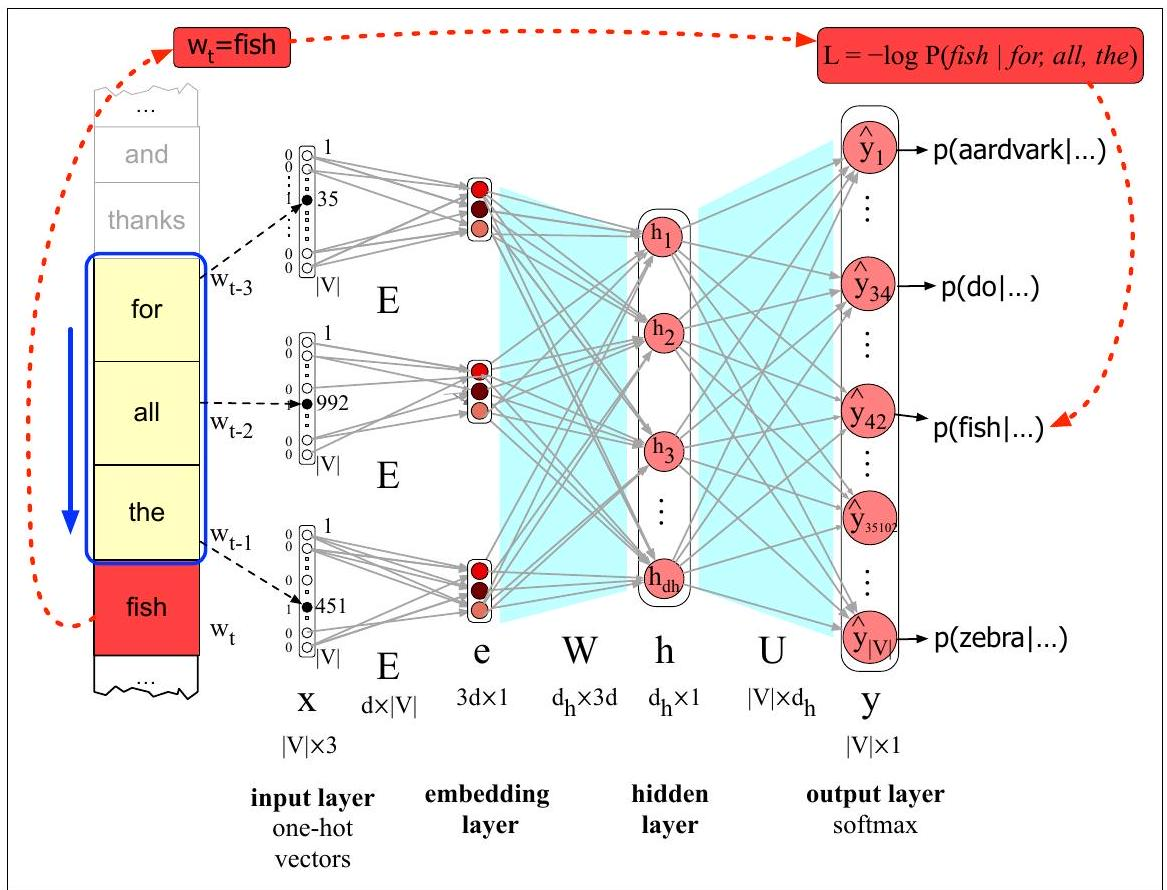
\includegraphics[max width=\textwidth, center]{2025_03_24_4f41283092a9d1f7a40eg-164}

Figure 7.18 Learning all the way back to embeddings. Again, the embedding matrix $\mathbf{E}$ is shared among the 3 context words.\\
is then:


\begin{equation*}
\theta^{s+1}=\theta^{s}-\eta \frac{\partial\left[-\log p\left(w_{t} \mid w_{t-1}, \ldots, w_{t-n+1}\right)\right]}{\partial \theta} \tag{7.46}
\end{equation*}


This gradient can be computed in any standard neural network framework which will then backpropagate through $\theta=\mathbf{E}, \mathbf{W}, \mathbf{U}, \mathbf{b}$.

Training the parameters to minimize loss will result both in an algorithm for language modeling (a word predictor) but also a new set of embeddings $\mathbf{E}$ that can be used as word representations for other tasks.

\subsection*{7.8 Summary}
\begin{itemize}
  \item Neural networks are built out of neural units, originally inspired by biological neurons but now simply an abstract computational device.
  \item Each neural unit multiplies input values by a weight vector, adds a bias, and then applies a non-linear activation function like sigmoid, tanh, or rectified linear unit.
  \item In a fully-connected, feedforward network, each unit in layer $i$ is connected to each unit in layer $i+1$, and there are no cycles.
  \item The power of neural networks comes from the ability of early layers to learn representations that can be utilized by later layers in the network.
  \item Neural networks are trained by optimization algorithms like gradient descent.
  \item Error backpropagation, backward differentiation on a computation graph, is used to compute the gradients of the loss function for a network.
  \item Neural language models use a neural network as a probabilistic classifier, to compute the probability of the next word given the previous $n$ words.
  \item Neural language models can use pretrained embeddings, or can learn embeddings from scratch in the process of language modeling.
\end{itemize}

\section*{Bibliographical and Historical Notes}
The origins of neural networks lie in the 1940s McCulloch-Pitts neuron (McCulloch and Pitts, 1943), a simplified model of the biological neuron as a kind of computing element that could be described in terms of propositional logic. By the late 1950s and early 1960s, a number of labs (including Frank Rosenblatt at Cornell and Bernard Widrow at Stanford) developed research into neural networks; this phase saw the development of the perceptron (Rosenblatt, 1958), and the transformation of the threshold into a bias, a notation we still use (Widrow and Hoff, 1960).

The field of neural networks declined after it was shown that a single perceptron unit was unable to model functions as simple as XOR (Minsky and Papert, 1969). While some small amount of work continued during the next two decades, a major revival for the field didn't come until the 1980s, when practical tools for building deeper networks like error backpropagation became widespread (Rumelhart et al., 1986). During the 1980s a wide variety of neural network and related architectures were developed, particularly for applications in psychology and cognitive science (Rumelhart and McClelland 1986b, McClelland and Elman 1986, Rumelhart and McClelland 1986a, Elman 1990), for which the term connectionist or parallel distributed processing was often used (Feldman and Ballard 1982, Smolensky 1988). Many of the principles and techniques developed in this period are foundational to modern work, including the ideas of distributed representations (Hinton, 1986), recurrent networks (Elman, 1990), and the use of tensors for compositionality (Smolensky, 1990).

By the 1990s larger neural networks began to be applied to many practical language processing tasks as well, like handwriting recognition (LeCun et al. 1989) and speech recognition (Morgan and Bourlard 1990). By the early 2000s, improvements in computer hardware and advances in optimization and training techniques made it possible to train even larger and deeper networks, leading to the modern term deep learning (Hinton et al. 2006, Bengio et al. 2007). We cover more related history in Chapter 8 and Chapter 16.

There are a number of excellent books on the subject. Goldberg (2017) has superb coverage of neural networks for natural language processing. For neural networks in general see Goodfellow et al. (2016) and Nielsen (2015).

Language is an inherently temporal phenomenon. Spoken language is a sequence of acoustic events over time, and we comprehend and produce both spoken and written language as a sequential input stream. The temporal nature of language is reflected in the metaphors we use; we talk of the flow of conversations, news feeds, and twitter streams, all of which emphasize that language is a sequence that unfolds in time.

Yet most of the machine learning approaches we've studied so far, like those for sentiment analysis and other text classification tasks don't have this temporal nature - they assume simultaneous access to all aspects of their input. The feedforward networks of Chapter 7 also assumed simultaneous access, although they also had a simple model for time. Recall that we applied feedforward networks to language modeling by having them look only at a fixed-size window of words, and then sliding this window over the input, making independent predictions along the way. This sliding-window approach is also used in the transformer architecture we will introduce in Chapter 9.

This chapter introduces a deep learning architecture that offers an alternative way of representing time: recurrent neural networks (RNNs), and their variants like LSTMs. RNNs have a mechanism that deals directly with the sequential nature of language, allowing them to handle the temporal nature of language without the use of arbitrary fixed-sized windows. The recurrent network offers a new way to represent the prior context, in its recurrent connections, allowing the model's decision to depend on information from hundreds of words in the past. We'll see how to apply the model to the task of language modeling, to text classification tasks like sentiment analysis, and to sequence modeling tasks like part-of-speech tagging (a task we'll return to in detail in Chapter 17).

\subsection*{8.1 Recurrent Neural Networks}
A recurrent neural network ( RNN ) is any network that contains a cycle within its network connections, meaning that the value of some unit is directly, or indirectly, dependent on its own earlier outputs as an input. While powerful, such networks are difficult to reason about and to train. However, within the general class of recurrent networks there are constrained architectures that have proven to be extremely effective when applied to language. In this section, we consider a class of recurrent networks referred to as Elman Networks (Elman, 1990) or simple recurrent networks. These networks are useful in their own right and serve as the basis for more complex approaches like the Long Short-Term Memory (LSTM) networks discussed\\
later in this chapter. In this chapter when we use the term RNN we'll be referring to these simpler more constrained networks (although you will often see the term RNN to mean any net with recurrent properties including LSTMs).\\
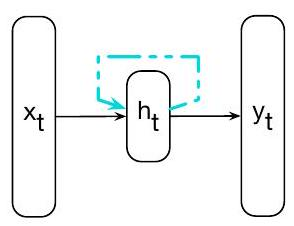
\includegraphics[max width=\textwidth, center]{2025_03_24_4f41283092a9d1f7a40eg-167}

Figure 8.1 Simple recurrent neural network after Elman (1990). The hidden layer includes a recurrent connection as part of its input. That is, the activation value of the hidden layer depends on the current input as well as the activation value of the hidden layer from the previous time step.

Fig. 8.1 illustrates the structure of an RNN. As with ordinary feedforward networks, an input vector representing the current input, $\mathbf{x}_{t}$, is multiplied by a weight matrix and then passed through a non-linear activation function to compute the values for a layer of hidden units. This hidden layer is then used to calculate a corresponding output, $\mathbf{y}_{t}$. In a departure from our earlier window-based approach, sequences are processed by presenting one item at a time to the network. We'll use subscripts to represent time, thus $\mathbf{x}_{t}$ will mean the input vector $\mathbf{x}$ at time $t$. The key difference from a feedforward network lies in the recurrent link shown in the figure with the dashed line. This link augments the input to the computation at the hidden layer with the value of the hidden layer from the preceding point in time.

The hidden layer from the previous time step provides a form of memory, or context, that encodes earlier processing and informs the decisions to be made at later points in time. Critically, this approach does not impose a fixed-length limit on this prior context; the context embodied in the previous hidden layer can include information extending back to the beginning of the sequence.

Adding this temporal dimension makes RNNs appear to be more complex than non-recurrent architectures. But in reality, they're not all that different. Given an input vector and the values for the hidden layer from the previous time step, we're still performing the standard feedforward calculation introduced in Chapter 7. To see this, consider Fig. 8.2 which clarifies the nature of the recurrence and how it factors into the computation at the hidden layer. The most significant change lies in the new set of weights, $\mathbf{U}$, that connect the hidden layer from the previous time step to the current hidden layer. These weights determine how the network makes use of past context in calculating the output for the current input. As with the other weights in the network, these connections are trained via backpropagation.

\subsection*{8.1.1 Inference in RNNs}
Forward inference (mapping a sequence of inputs to a sequence of outputs) in an RNN is nearly identical to what we've already seen with feedforward networks. To compute an output $\mathbf{y}_{t}$ for an input $\mathbf{x}_{t}$, we need the activation value for the hidden layer $\mathbf{h}_{t}$. To calculate this, we multiply the input $\mathbf{x}_{t}$ with the weight matrix $\mathbf{W}$, and the hidden layer from the previous time step $\mathbf{h}_{t-1}$ with the weight matrix $\mathbf{U}$. We add these values together and pass them through a suitable activation function, $g$, to arrive at the activation value for the current hidden layer, $\mathbf{h}_{t}$. Once we have the values for the hidden layer, we proceed with the usual computation to generate the\\
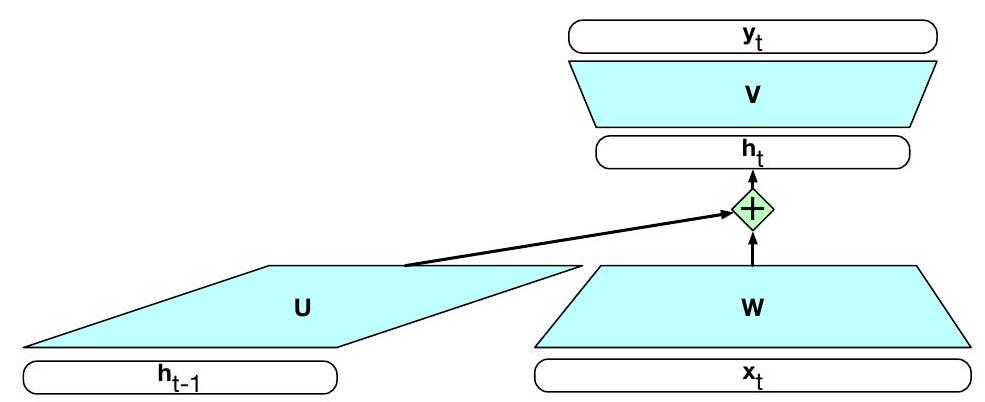
\includegraphics[max width=\textwidth, center]{2025_03_24_4f41283092a9d1f7a40eg-168}

Figure 8.2 Simple recurrent neural network illustrated as a feedforward network. The hidden layer $\mathbf{h}_{t-1}$ from the prior time step is multiplied by weight matrix $\mathbf{U}$ and then added to the feedforward component from the current time step.\\
output vector.


\begin{align*}
\mathbf{h}_{t} & =g\left(\mathbf{U h}_{t-1}+\mathbf{W} \mathbf{x}_{t}\right)  \tag{8.1}\\
\mathbf{y}_{t} & =f\left(\mathbf{V h}_{t}\right) \tag{8.2}
\end{align*}


Let's refer to the input, hidden and output layer dimensions as $d_{i n}, d_{h}$, and $d_{\text {out }}$ respectively. Given this, our three parameter matrices are: $W \in \mathbb{R}^{d_{h} \times d_{i n}}, \mathbf{U} \in \mathbb{R}^{d_{h} \times d_{h}}$, and $\mathbf{V} \in \mathbb{R}^{d_{\text {out }} \times d_{h}}$.

We compute $y_{t}$ via a softmax computation that gives a probability distribution over the possible output classes.


\begin{equation*}
\mathbf{y}_{t}=\operatorname{softmax}\left(\mathbf{V} \mathbf{h}_{t}\right) \tag{8.3}
\end{equation*}


The fact that the computation at time $t$ requires the value of the hidden layer from time $t-1$ mandates an incremental inference algorithm that proceeds from the start of the sequence to the end as illustrated in Fig. 8.3. The sequential nature of simple recurrent networks can also be seen by unrolling the network in time as is shown in Fig. 8.4. In this figure, the various layers of units are copied for each time step to illustrate that they will have differing values over time. However, the various weight matrices are shared across time.

\begin{verbatim}
function FORWARDRNN(x, network) returns output sequence y
    h
    for i\leftarrow1 to LENGTH(\mathbf{x}) do
        \mp@subsup{\mathbf{h}}{i}{}\leftarrowg(\mathbf{Uh}
        \mp@subsup{\mathbf{y}}{i}{}\leftarrowf(\mathbf{Vh}
    return y
\end{verbatim}

Figure 8.3 Forward inference in a simple recurrent network. The matrices $\mathbf{U}, \mathbf{V}$ and $\mathbf{W}$ are shared across time, while new values for $\mathbf{h}$ and $\mathbf{y}$ are calculated with each time step.

\subsection*{8.1.2 Training}
As with feedforward networks, we'll use a training set, a loss function, and backpropagation to obtain the gradients needed to adjust the weights in these recurrent networks. As shown in Fig. 8.2, we now have 3 sets of weights to update: W, the\\
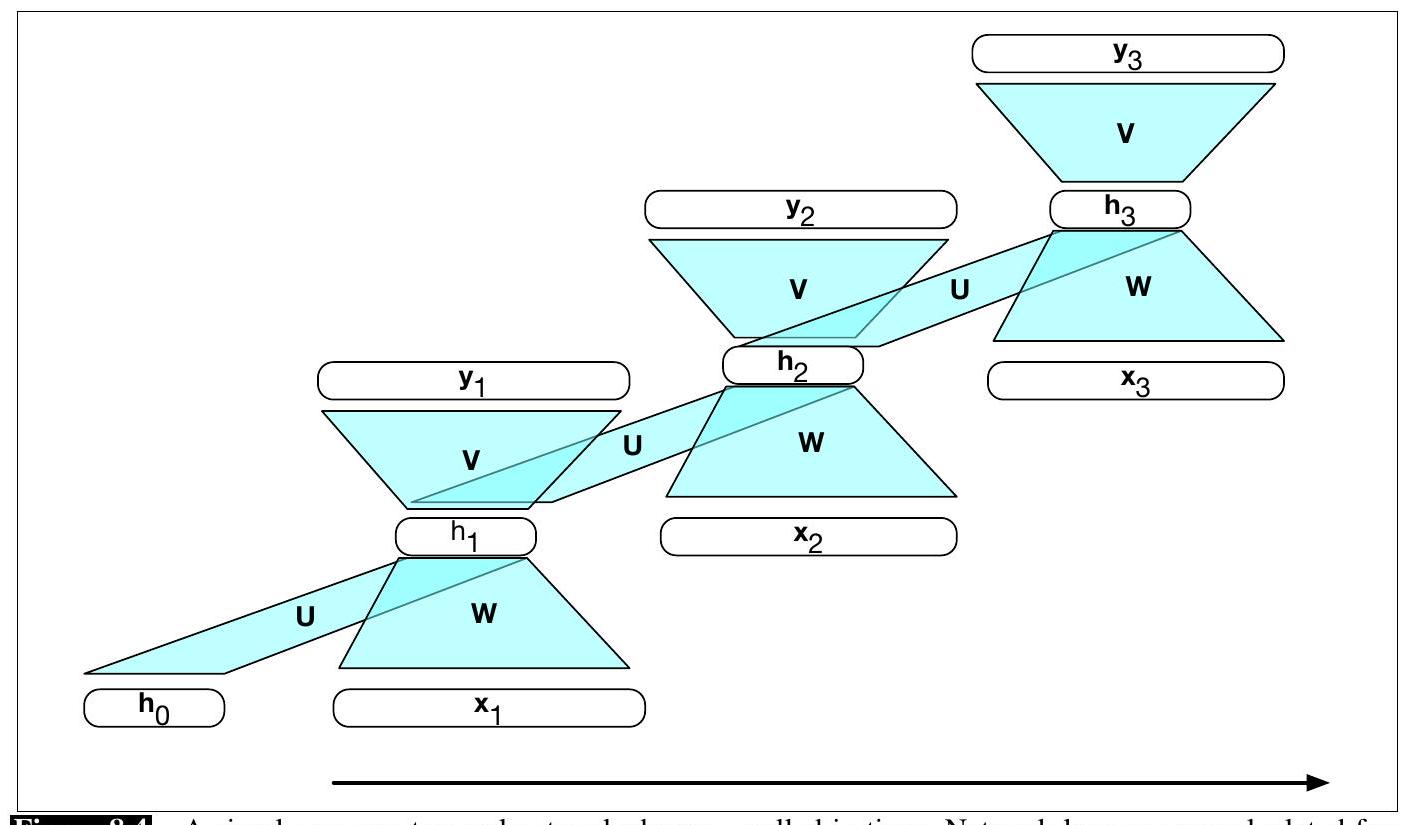
\includegraphics[max width=\textwidth, center]{2025_03_24_4f41283092a9d1f7a40eg-169}

Figure 8.4 A simple recurrent neural network shown unrolled in time. Network layers are recalculated for each time step, while the weights $\mathbf{U}, \mathbf{V}$ and $\mathbf{W}$ are shared across all time steps.\\
weights from the input layer to the hidden layer, $\mathbf{U}$, the weights from the previous hidden layer to the current hidden layer, and finally $\mathbf{V}$, the weights from the hidden layer to the output layer.

Fig. 8.4 highlights two considerations that we didn't have to worry about with backpropagation in feedforward networks. First, to compute the loss function for the output at time $t$ we need the hidden layer from time $t-1$. Second, the hidden layer at time $t$ influences both the output at time $t$ and the hidden layer at time $t+1$ (and hence the output and loss at $t+1$ ). It follows from this that to assess the error accruing to $\mathbf{h}_{t}$, we'll need to know its influence on both the current output as well as the ones that follow.

Tailoring the backpropagation algorithm to this situation leads to a two-pass algorithm for training the weights in RNNs. In the first pass, we perform forward inference, computing $\mathbf{h}_{t}, \mathbf{y}_{t}$, accumulating the loss at each step in time, saving the value of the hidden layer at each step for use at the next time step. In the second phase, we process the sequence in reverse, computing the required gradients as we go, computing and saving the error term for use in the hidden layer for each step backward in time. This general approach is commonly referred to as backpropagation through time (Werbos 1974, Rumelhart et al. 1986, Werbos 1990).

Fortunately, with modern computational frameworks and adequate computing resources, there is no need for a specialized approach to training RNNs. As illustrated in Fig. 8.4, explicitly unrolling a recurrent network into a feedforward computational graph eliminates any explicit recurrences, allowing the network weights to be trained directly. In such an approach, we provide a template that specifies the basic structure of the network, including all the necessary parameters for the input, output, and hidden layers, the weight matrices, as well as the activation and output functions to be used. Then, when presented with a specific input sequence, we can generate an unrolled feedforward network specific to that input, and use that graph to perform forward inference or training via ordinary backpropagation.

For applications that involve much longer input sequences, such as speech recognition, character-level processing, or streaming continuous inputs, unrolling an entire input sequence may not be feasible. In these cases, we can unroll the input into manageable fixed-length segments and treat each segment as a distinct training item.

\subsection*{8.2 RNNs as Language Models}
Let's see how to apply RNNs to the language modeling task. Recall from Chapter 3 that language models predict the next word in a sequence given some preceding context. For example, if the preceding context is "Thanks for all the" and we want to know how likely the next word is "fish" we would compute:

$$
P(f i s h \mid T h a n k s \text { for all the })
$$

Language models give us the ability to assign such a conditional probability to every possible next word, giving us a distribution over the entire vocabulary. We can also assign probabilities to entire sequences by combining these conditional probabilities with the chain rule:

$$
P\left(w_{1: n}\right)=\prod_{i=1}^{n} P\left(w_{i} \mid w_{<i}\right)
$$

The n-gram language models of Chapter 3 compute the probability of a word given counts of its occurrence with the $n-1$ prior words. The context is thus of size $n-1$. For the feedforward language models of Chapter 7, the context is the window size.

RNN language models (Mikolov et al., 2010) process the input sequence one word at a time, attempting to predict the next word from the current word and the previous hidden state. RNNs thus don't have the limited context problem that n-gram models have, or the fixed context that feedforward language models have, since the hidden state can in principle represent information about all of the preceding words all the way back to the beginning of the sequence. Fig. 8.5 sketches this difference between a FFN language model and an RNN language model, showing that the RNN language model uses $h_{t-1}$, the hidden state from the previous time step, as a representation of the past context.

\subsection*{8.2.1 Forward Inference in an RNN language model}
Forward inference in a recurrent language model proceeds exactly as described in Section 8.1.1. The input sequence $\mathbf{X}=\left[\mathbf{x}_{1} ; \ldots ; \mathbf{x}_{t} ; \ldots ; \mathbf{x}_{N}\right]$ consists of a series of words each represented as a one-hot vector of size $|V| \times 1$, and the output prediction, $\mathbf{y}$, is a vector representing a probability distribution over the vocabulary. At each step, the model uses the word embedding matrix $\mathbf{E}$ to retrieve the embedding for the current word, multiples it by the weight matrix $\mathbf{W}$, and then adds it to the hidden layer from the previous step (weighted by weight matrix $\mathbf{U}$ ) to compute a new hidden layer. This hidden layer is then used to generate an output layer which is passed through a softmax layer to generate a probability distribution over the entire vocabulary. That is, at time $t$ :


\begin{align*}
\mathbf{e}_{t} & =\mathbf{E x}_{t}  \tag{8.4}\\
\mathbf{h}_{t} & =g\left(\mathbf{U h}_{t-1}+\mathbf{W} \mathbf{e}_{t}\right)  \tag{8.5}\\
\hat{\mathbf{y}}_{t} & =\operatorname{softmax}\left(\mathbf{V} \mathbf{h}_{t}\right) \tag{8.6}
\end{align*}


\begin{center}
\includegraphics[max width=\textwidth]{2025_03_24_4f41283092a9d1f7a40eg-171}
\end{center}

Figure 8.5 Simplified sketch of two LM architectures moving through a text, showing a schematic context of three tokens: (a) a feedforward neural language model which has a fixed context input to the weight matrix $\mathbf{W}$, (b) an RNN language model, in which the hidden state $\mathbf{h}_{t-1}$ summarizes the prior context.

When we do language modeling with RNNs (and we'll see this again in Chapter 9 with transformers), it's convenient to make the assumption that the embedding dimension $d_{e}$ and the hidden dimension $d_{h}$ are the same. So we'll just call both of these the model dimension $d$. So the embedding matrix $\mathbf{E}$ is of shape $[d \times|V|]$, and $\mathbf{x}_{\mathbf{t}}$ is a one-hot vector of shape $[|V| \times 1]$. The product $\mathbf{e}_{t}$ is thus of shape $[d \times 1]$. W and $\mathbf{U}$ are of shape $[d \times d]$, so $\mathbf{h}_{t}$ is also of shape $[d \times 1]$. $\mathbf{V}$ is of shape $[|V| \times d]$, so the result of $\mathbf{V h}$ is a vector of shape $[|V| \times 1]$. This vector can be thought of as a set of scores over the vocabulary given the evidence provided in $\mathbf{h}$. Passing these scores through the softmax normalizes the scores into a probability distribution. The probability that a particular word $k$ in the vocabulary is the next word is represented by $\hat{\mathbf{y}}_{t}[k]$, the $k$ th component of $\hat{\mathbf{y}}_{t}$ :


\begin{equation*}
P\left(w_{t+1}=k \mid w_{1}, \ldots, w_{t}\right)=\hat{\mathbf{y}}_{t}[k] \tag{8.7}
\end{equation*}


The probability of an entire sequence is just the product of the probabilities of each item in the sequence, where we'll use $\hat{\mathbf{y}}_{i}\left[w_{i}\right]$ to mean the probability of the true word $w_{i}$ at time step $i$.


\begin{align*}
P\left(w_{1: n}\right) & =\prod_{i=1}^{n} P\left(w_{i} \mid w_{1: i-1}\right)  \tag{8.8}\\
& =\prod_{i=1}^{n} \hat{\mathbf{y}}_{i}\left[w_{i}\right] \tag{8.9}
\end{align*}


\subsection*{8.2.2 Training an RNN language model}
To train an RNN as a language model, we use the same self-supervision (or selftraining) algorithm we saw in Section 7.7: we take a corpus of text as training material and at each time step $t$ ask the model to predict the next word. We call such a model self-supervised because we don't have to add any special gold labels to the data; the natural sequence of words is its own supervision! We simply train the model to minimize the error in predicting the true next word in the training sequence, using cross-entropy as the loss function. Recall that the cross-entropy loss measures the difference between a predicted probability distribution and the\\
\includegraphics[max width=\textwidth, center]{2025_03_24_4f41283092a9d1f7a40eg-172}

Figure 8.6 Training RNNs as language models.\\
correct distribution.


\begin{equation*}
L_{C E}=-\sum_{w \in V} \mathbf{y}_{t}[w] \log \hat{\mathbf{y}}_{t}[w] \tag{8.10}
\end{equation*}


In the case of language modeling, the correct distribution $\mathbf{y}_{t}$ comes from knowing the next word. This is represented as a one-hot vector corresponding to the vocabulary where the entry for the actual next word is 1 , and all the other entries are 0 . Thus, the cross-entropy loss for language modeling is determined by the probability the model assigns to the correct next word. So at time $t$ the CE loss is the negative log probability the model assigns to the next word in the training sequence.


\begin{equation*}
L_{C E}\left(\hat{\mathbf{y}}_{t}, \mathbf{y}_{t}\right)=-\log \hat{\mathbf{y}}_{t}\left[w_{t+1}\right] \tag{8.11}
\end{equation*}


Thus at each word position $t$ of the input, the model takes as input the correct word $w_{t}$ together with $h_{t-1}$, encoding information from the preceding $w_{1: t-1}$, and uses them to compute a probability distribution over possible next words so as to compute the model's loss for the next token $w_{t+1}$. Then we move to the next word, we ignore what the model predicted for the next word and instead use the correct word $w_{t+1}$ along with the prior history encoded to estimate the probability of token $w_{t+2}$. This idea that we always give the model the correct history sequence to predict the next word (rather than feeding the model its best case from the previous time step) is called teacher forcing.

The weights in the network are adjusted to minimize the average CE loss over the training sequence via gradient descent. Fig. 8.6 illustrates this training regimen.

\subsection*{8.2.3 Weight Tying}
Careful readers may have noticed that the input embedding matrix $\mathbf{E}$ and the final layer matrix $\mathbf{V}$, which feeds the output softmax, are quite similar.

The columns of $\mathbf{E}$ represent the word embeddings for each word in the vocabulary learned during the training process with the goal that words that have similar meaning and function will have similar embeddings. And, since when we use RNNs for language modeling we make the assumption that the embedding dimension and\\
the hidden dimension are the same (= the model dimension $d$ ), the embedding matrix $\mathbf{E}$ has shape $[d \times|V|]$. And the final layer matrix $\mathbf{V}$ provides a way to score the likelihood of each word in the vocabulary given the evidence present in the final hidden layer of the network through the calculation of $\mathbf{V h} . \mathbf{V}$ is of shape $[|V| \times d]$. That is, is, the rows of $\mathbf{V}$ are shaped like a transpose of $\mathbf{E}$, meaning that $\mathbf{V}$ provides a second set of learned word embeddings.

Instead of having two sets of embedding matrices, language models use a single embedding matrix, which appears at both the input and softmax layers. That is, we dispense with $\mathbf{V}$ and use $\mathbf{E}$ at the start of the computation and $\mathbf{E}^{\top}$ (because the shape of $\mathbf{V}$ is the transpose of $\mathbf{E}$ at the end. Using the same matrix (transposed) in\\
weight tying two places is called weight tying. ${ }^{1}$ The weight-tied equations for an RNN language model then become:


\begin{align*}
\mathbf{e}_{t} & =\mathbf{E x}_{t}  \tag{8.12}\\
\mathbf{h}_{t} & =g\left(\mathbf{U} \mathbf{h}_{t-1}+\mathbf{W} \mathbf{e}_{t}\right)  \tag{8.13}\\
\hat{\mathbf{y}}_{t} & =\operatorname{softmax}\left(\mathbf{E}^{\top} \mathbf{h}_{t}\right) \tag{8.14}
\end{align*}


In addition to providing improved model perplexity, this approach significantly reduces the number of parameters required for the model.

\subsection*{8.3 RNNs for other NLP tasks}
Now that we've seen the basic RNN architecture, let's consider how to apply it to three types of NLP tasks: sequence classification tasks like sentiment analysis and topic classification, sequence labeling tasks like part-of-speech tagging, and text generation tasks, including with a new architecture called the encoder-decoder.

\subsection*{8.3.1 Sequence Labeling}
In sequence labeling, the network's task is to assign a label chosen from a small fixed set of labels to each element of a sequence. One classic sequence labeling tasks is part-of-speech (POS) tagging (assigning grammatical tags like NOUN and VERB to each word in a sentence). We'll discuss part-of-speech tagging in detail in Chapter 17, but let's give a motivating example here. In an RNN approach to sequence labeling, inputs are word embeddings and the outputs are tag probabilities generated by a softmax layer over the given tagset, as illustrated in Fig. 8.7.

In this figure, the inputs at each time step are pretrained word embeddings corresponding to the input tokens. The RNN block is an abstraction that represents an unrolled simple recurrent network consisting of an input layer, hidden layer, and output layer at each time step, as well as the shared $\mathbf{U}, \mathbf{V}$ and $\mathbf{W}$ weight matrices that comprise the network. The outputs of the network at each time step represent the distribution over the POS tagset generated by a softmax layer.

To generate a sequence of tags for a given input, we run forward inference over the input sequence and select the most likely tag from the softmax at each step. Since we're using a softmax layer to generate the probability distribution over the output tagset at each time step, we will again employ the cross-entropy loss during training.

\footnotetext{1 We also do this for transformers (Chapter 9) where it's common to call $\mathbf{E}^{\top}$ the unembedding matrix.
}
\includegraphics[max width=\textwidth, center]{2025_03_24_4f41283092a9d1f7a40eg-174}

Figure 8.7 Part-of-speech tagging as sequence labeling with a simple RNN. The goal of part-of-speech (POS) tagging is to assign a grammatical label to each word in a sentence, drawn from a predefined set of tags. (The tags for this sentence include NNP (proper noun), MD (modal verb) and others; we'll give a complete description of the task of part-of-speech tagging in Chapter 17.) Pre-trained word embeddings serve as inputs and a softmax layer provides a probability distribution over the part-of-speech tags as output at each time step.

\subsection*{8.3.2 RNNs for Sequence Classification}
Another use of RNNs is to classify entire sequences rather than the tokens within them. This is the set of tasks commonly called text classification, like sentiment analysis or spam detection, in which we classify a text into two or three classes (like positive or negative), as well as classification tasks with a large number of categories, like document-level topic classification, or message routing for customer service applications.

To apply RNNs in this setting, we pass the text to be classified through the RNN a word at a time generating a new hidden layer representation at each time step. We can then take the hidden layer for the last token of the text, $\mathbf{h}_{n}$, to constitute a compressed representation of the entire sequence. We can pass this representation $\mathbf{h}_{n}$ to a feedforward network that chooses a class via a softmax over the possible classes. Fig. 8.8 illustrates this approach.

Note that in this approach we don't need intermediate outputs for the words in the sequence preceding the last element. Therefore, there are no loss terms associated with those elements. Instead, the loss function used to train the weights in the network is based entirely on the final text classification task. The output from the softmax output from the feedforward classifier together with a cross-entropy loss drives the training. The error signal from the classification is backpropagated all the way through the weights in the feedforward classifier through, to its input, and then through to the three sets of weights in the RNN as described earlier in Section 8.1.2. The training regimen that uses the loss from a downstream application to adjust the weights all the way through the network is referred to as end-to-end training.

Another option, instead of using just hidden state of the last token $h_{n}$ to represent the whole sequence, is to use some sort of pooling function of all the hidden states $h_{i}$ for each word $i$ in the sequence. For example, we can create a representation that\\
\includegraphics[max width=\textwidth, center]{2025_03_24_4f41283092a9d1f7a40eg-175}

Figure 8.8 Sequence classification using a simple RNN combined with a feedforward network. The final hidden state from the RNN is used as the input to a feedforward network that performs the classification.\\
pools all the $n$ hidden states by taking their element-wise mean:


\begin{equation*}
\mathbf{h}_{\text {mean }}=\frac{1}{n} \sum_{i=1}^{n} \mathbf{h}_{i} \tag{8.15}
\end{equation*}


Or we can take the element-wise max; the element-wise max of a set of $n$ vectors is a new vector whose $k$ th element is the max of the $k$ th elements of all the $n$ vectors.

The long contexts of RNNs makes it quite difficult to successfully backpropagate error all the way through the entire input; we'll talk about this problem, and some standard solutions, in Section 8.5.

\subsection*{8.3.3 Generation with RNN-Based Language Models}
RNN-based language models can also be used to generate text. Text generation is of enormous practical importance, part of tasks like question answering, machine translation, text summarization, grammar correction, story generation, and conversational dialogue; any task where a system needs to produce text, conditioned on some other text. This use of a language model to generate text is one of the areas in which the impact of neural language models on NLP has been the largest. Text generation, along with image generation and code generation, constitute a new area of AI that is often called generative AI.

Recall back in Chapter 3 we saw how to generate text from an n-gram language model by adapting a sampling technique suggested at about the same time by Claude Shannon (Shannon, 1951) and the psychologists George Miller and Jennifer Selfridge (Miller and Selfridge, 1950). We first randomly sample a word to begin a sequence based on its suitability as the start of a sequence. We then continue to sample words conditioned on our previous choices until we reach a pre-determined length, or an end of sequence token is generated.

Today, this approach of using a language model to incrementally generate words by repeatedly sampling the next word conditioned on our previous choices is called the same as that described on page 43, but adapted to a neural context:

\begin{itemize}
  \item Sample a word in the output from the softmax distribution that results from using the beginning of sentence marker, <s>, as the first input.
  \item Use the word embedding for that first word as the input to the network at the next time step, and then sample the next word in the same fashion.
  \item Continue generating until the end of sentence marker, </s>, is sampled or a fixed length limit is reached.\\
Technically an autoregressive model is a model that predicts a value at time $t$ based on a linear function of the previous values at times $t-1, t-2$, and so on. Although language models are not linear (since they have many layers of non-linearities), we loosely refer to this generation technique as autoregressive generation since the word generated at each time step is conditioned on the word selected by the network from the previous step. Fig. 8.9 illustrates this approach. In this figure, the details of the RNN's hidden layers and recurrent connections are hidden within the blue block.
\end{itemize}

This simple architecture underlies state-of-the-art approaches to applications such as machine translation, summarization, and question answering. The key to these approaches is to prime the generation component with an appropriate context. That is, instead of simply using <s> to get things started we can provide a richer task-appropriate context; for translation the context is the sentence in the source language; for summarization it's the long text we want to summarize.\\
\includegraphics[max width=\textwidth, center]{2025_03_24_4f41283092a9d1f7a40eg-176}

Figure 8.9 Autoregressive generation with an RNN-based neural language model.

\subsection*{8.4 Stacked and Bidirectional RNN architectures}
Recurrent networks are quite flexible. By combining the feedforward nature of unrolled computational graphs with vectors as common inputs and outputs, complex networks can be treated as modules that can be combined in creative ways. This section introduces two of the more common network architectures used in language processing with RNNs.

\subsection*{8.4.1 Stacked RNNs}
In our examples thus far, the inputs to our RNNs have consisted of sequences of word or character embeddings (vectors) and the outputs have been vectors useful for predicting words, tags or sequence labels. However, nothing prevents us from using\\
the entire sequence of outputs from one RNN as an input sequence to another one.\\
Stacked RNNs consist of multiple networks where the output of one layer serves as the input to a subsequent layer, as shown in Fig. 8.10.\\
\includegraphics[max width=\textwidth, center]{2025_03_24_4f41283092a9d1f7a40eg-177}

Figure 8.10 Stacked recurrent networks. The output of a lower level serves as the input to higher levels with the output of the last network serving as the final output.

Stacked RNNs generally outperform single-layer networks. One reason for this success seems to be that the network induces representations at differing levels of abstraction across layers. Just as the early stages of the human visual system detect edges that are then used for finding larger regions and shapes, the initial layers of stacked networks can induce representations that serve as useful abstractions for further layers-representations that might prove difficult to induce in a single RNN. The optimal number of stacked RNNs is specific to each application and to each training set. However, as the number of stacks is increased the training costs rise quickly.

\subsection*{8.4.2 Bidirectional RNNs}
The RNN uses information from the left (prior) context to make its predictions at time $t$. But in many applications we have access to the entire input sequence; in those cases we would like to use words from the context to the right of $t$. One way to do this is to run two separate RNNs, one left-to-right, and one right-to-left, and concatenate their representations.

In the left-to-right RNNs we've discussed so far, the hidden state at a given time $t$ represents everything the network knows about the sequence up to that point. The state is a function of the inputs $x_{1}, \ldots, x_{t}$ and represents the context of the network to the left of the current time.


\begin{equation*}
\mathbf{h}_{t}^{f}=\mathrm{RNN}_{\text {forward }}\left(\mathbf{x}_{1}, \ldots, \mathbf{x}_{t}\right) \tag{8.16}
\end{equation*}


This new notation $\mathbf{h}_{t}^{f}$ simply corresponds to the normal hidden state at time $t$, representing everything the network has gleaned from the sequence so far.

To take advantage of context to the right of the current input, we can train an RNN on a reversed input sequence. With this approach, the hidden state at time $t$ represents information about the sequence to the right of the current input:


\begin{equation*}
\mathbf{h}_{t}^{b}=\mathrm{RNN}_{\text {backward }}\left(\mathbf{x}_{t}, \ldots \mathbf{x}_{n}\right) \tag{8.17}
\end{equation*}


Here, the hidden state $\mathbf{h}_{t}^{b}$ represents all the information we have discerned about the sequence from $t$ to the end of the sequence.

A bidirectional RNN (Schuster and Paliwal, 1997) combines two independent RNNs, one where the input is processed from the start to the end, and the other from the end to the start. We then concatenate the two representations computed by the networks into a single vector that captures both the left and right contexts of an input at each point in time. Here we use either the semicolon ";" or the equivalent symbol $\oplus$ to mean vector concatenation:


\begin{align*}
\mathbf{h}_{t} & =\left[\mathbf{h}_{t}^{f} ; \mathbf{h}_{t}^{b}\right] \\
& =\mathbf{h}_{t}^{f} \oplus \mathbf{h}_{t}^{b} \tag{8.18}
\end{align*}


Fig. 8.11 illustrates such a bidirectional network that concatenates the outputs of the forward and backward pass. Other simple ways to combine the forward and backward contexts include element-wise addition or multiplication. The output at each step in time thus captures information to the left and to the right of the current input. In sequence labeling applications, these concatenated outputs can serve as the basis for a local labeling decision.\\
\includegraphics[max width=\textwidth, center]{2025_03_24_4f41283092a9d1f7a40eg-178}

Figure 8.11 A bidirectional RNN. Separate models are trained in the forward and backward directions, with the output of each model at each time point concatenated to represent the bidirectional state at that time point.

Bidirectional RNNs have also proven to be quite effective for sequence classification. Recall from Fig. 8.8 that for sequence classification we used the final hidden state of the RNN as the input to a subsequent feedforward classifier. A difficulty with this approach is that the final state naturally reflects more information about the end of the sentence than its beginning. Bidirectional RNNs provide a simple solution to this problem; as shown in Fig. 8.12, we simply combine the final hidden states from the forward and backward passes (for example by concatenation) and use that as input for follow-on processing.\\
\includegraphics[max width=\textwidth, center]{2025_03_24_4f41283092a9d1f7a40eg-179}

Figure 8.12 A bidirectional RNN for sequence classification. The final hidden units from the forward and backward passes are combined to represent the entire sequence. This combined representation serves as input to the subsequent classifier.

\subsection*{8.5 The LSTM}
In practice, it is quite difficult to train RNNs for tasks that require a network to make use of information distant from the current point of processing. Despite having access to the entire preceding sequence, the information encoded in hidden states tends to be fairly local, more relevant to the most recent parts of the input sequence and recent decisions. Yet distant information is critical to many language applications. Consider the following example in the context of language modeling.\\
(8.19) The flights the airline was canceling were full.

Assigning a high probability to was following airline is straightforward since airline provides a strong local context for the singular agreement. However, assigning an appropriate probability to were is quite difficult, not only because the plural flights is quite distant, but also because the singular noun airline is closer in the intervening context. Ideally, a network should be able to retain the distant information about plural flights until it is needed, while still processing the intermediate parts of the sequence correctly.

One reason for the inability of RNNs to carry forward critical information is that the hidden layers, and, by extension, the weights that determine the values in the hidden layer, are being asked to perform two tasks simultaneously: provide information useful for the current decision, and updating and carrying forward information required for future decisions.

A second difficulty with training RNNs arises from the need to backpropagate the error signal back through time. Recall from Section 8.1.2 that the hidden layer at time $t$ contributes to the loss at the next time step since it takes part in that calculation. As a result, during the backward pass of training, the hidden layers are subject to repeated multiplications, as determined by the length of the sequence. A frequent result of this process is that the gradients are eventually driven to zero, a situation\\
vanishing gradients\\
called the vanishing gradients problem.\\
To address these issues, more complex network architectures have been designed to explicitly manage the task of maintaining relevant context over time, by enabling the network to learn to forget information that is no longer needed and to remember information required for decisions still to come.

The most commonly used such extension to RNNs is the long short-term memory (LSTM) network (Hochreiter and Schmidhuber, 1997). LSTMs divide the context management problem into two subproblems: removing information no longer needed from the context, and adding information likely to be needed for later decision making. The key to solving both problems is to learn how to manage this context rather than hard-coding a strategy into the architecture. LSTMs accomplish this by first adding an explicit context layer to the architecture (in addition to the usual recurrent hidden layer), and through the use of specialized neural units that make use of gates to control the flow of information into and out of the units that comprise the network layers. These gates are implemented through the use of additional weights that operate sequentially on the input, and previous hidden layer, and previous context layers.

The gates in an LSTM share a common design pattern; each consists of a feedforward layer, followed by a sigmoid activation function, followed by a pointwise multiplication with the layer being gated. The choice of the sigmoid as the activation function arises from its tendency to push its outputs to either 0 or 1 . Combining this with a pointwise multiplication has an effect similar to that of a binary mask. Values in the layer being gated that align with values near 1 in the mask are passed through nearly unchanged; values corresponding to lower values are essentially erased.

The first gate we'll consider is the forget gate. The purpose of this gate is to delete information from the context that is no longer needed. The forget gate computes a weighted sum of the previous state's hidden layer and the current input and passes that through a sigmoid. This mask is then multiplied element-wise by the context vector to remove the information from context that is no longer required. Element-wise multiplication of two vectors (represented by the operator $\odot$, and sometimes called the Hadamard product) is the vector of the same dimension as the two input vectors, where each element $i$ is the product of element $i$ in the two input vectors:


\begin{align*}
\mathbf{f}_{t} & =\sigma\left(\mathbf{U}_{f} \mathbf{h}_{t-1}+\mathbf{W}_{f} \mathbf{x}_{t}\right)  \tag{8.20}\\
\mathbf{k}_{t} & =\mathbf{c}_{t-1} \odot \mathbf{f}_{t} \tag{8.21}
\end{align*}


The next task is to compute the actual information we need to extract from the previous hidden state and current inputs-the same basic computation we've been using for all our recurrent networks.


\begin{equation*}
\mathbf{g}_{t}=\tanh \left(\mathbf{U}_{g} \mathbf{h}_{t-1}+\mathbf{W}_{g} \mathbf{x}_{t}\right) \tag{8.22}
\end{equation*}


Next, we generate the mask for the add gate to select the information to add to the current context.


\begin{align*}
& \mathbf{i}_{t}=\sigma\left(\mathbf{U}_{i} \mathbf{h}_{t-1}+\mathbf{W}_{i} \mathbf{x}_{t}\right)  \tag{8.23}\\
& \mathbf{j}_{t}=\mathbf{g}_{t} \odot \mathbf{i}_{t} \tag{8.24}
\end{align*}


Next, we add this to the modified context vector to get our new context vector.


\begin{equation*}
\mathbf{c}_{t}=\mathbf{j}_{t}+\mathbf{k}_{t} \tag{8.25}
\end{equation*}


\begin{center}
\includegraphics[max width=\textwidth]{2025_03_24_4f41283092a9d1f7a40eg-181}
\end{center}

Figure 8.13 A single LSTM unit displayed as a computation graph. The inputs to each unit consists of the current input, $x$, the previous hidden state, $h_{t-1}$, and the previous context, $c_{t-1}$. The outputs are a new hidden state, $h_{t}$ and an updated context, $c_{t}$.\\
output gate\\
The final gate we'll use is the output gate which is used to decide what information is required for the current hidden state (as opposed to what information needs to be preserved for future decisions).


\begin{align*}
& \mathbf{o}_{t}=\sigma\left(\mathbf{U}_{o} \mathbf{h}_{t-1}+\mathbf{W}_{o} \mathbf{x}_{t}\right)  \tag{8.26}\\
& \mathbf{h}_{t}=\mathbf{o}_{t} \odot \tanh \left(\mathbf{c}_{t}\right) \tag{8.27}
\end{align*}


Fig. 8.13 illustrates the complete computation for a single LSTM unit. Given the appropriate weights for the various gates, an LSTM accepts as input the context layer, and hidden layer from the previous time step, along with the current input vector. It then generates updated context and hidden vectors as output.

It is the hidden state, $h_{t}$, that provides the output for the LSTM at each time step. This output can be used as the input to subsequent layers in a stacked RNN, or at the final layer of a network $h_{t}$ can be used to provide the final output of the LSTM.

\subsection*{8.5.1 Gated Units, Layers and Networks}
The neural units used in LSTMs are obviously much more complex than those used in basic feedforward networks. Fortunately, this complexity is encapsulated within the basic processing units, allowing us to maintain modularity and to easily experiment with different architectures. To see this, consider Fig. 8.14 which illustrates the inputs and outputs associated with each kind of unit.

At the far left, (a) is the basic feedforward unit where a single set of weights and a single activation function determine its output, and when arranged in a layer there are no connections among the units in the layer. Next, (b) represents the unit in a simple recurrent network. Now there are two inputs and an additional set of weights to go with it. However, there is still a single activation function and output.

The increased complexity of the LSTM units is encapsulated within the unit itself. The only additional external complexity for the LSTM over the basic recurrent unit (b) is the presence of the additional context vector as an input and output.

This modularity is key to the power and widespread applicability of LSTM units. LSTM units (or other varieties, like GRUs) can be substituted into any of the network architectures described in Section 8.4. And, as with simple RNNs, multi-layered networks making use of gated units can be unrolled into deep feedforward networks\\
\includegraphics[max width=\textwidth, center]{2025_03_24_4f41283092a9d1f7a40eg-182}

Figure 8.14 Basic neural units used in feedforward, simple recurrent networks (SRN), and long short-term memory (LSTM).\\
and trained in the usual fashion with backpropagation. In practice, therefore, LSTMs rather than RNNs have become the standard unit for any modern system that makes use of recurrent networks.

\subsection*{8.6 Summary: Common RNN NLP Architectures}
We've now introduced the RNN, seen advanced components like stacking multiple layers and using the LSTM version, and seen how the RNN can be applied to various tasks. Let's take a moment to summarize the architectures for these applications.

Fig. 8.15 shows the three architectures we've discussed so far: sequence labeling, sequence classification, and language modeling. In sequence labeling (for example for part of speech tagging), we train a model to produce a label for each input word or token. In sequence classification, for example for sentiment analysis, we ignore the output for each token, and only take the value from the end of the sequence (and similarly the model's training signal comes from backpropagation from that last token). In language modeling, we train the model to predict the next word at each token step. In the next section we'll introduce a fourth architecture, the encoder-decoder.

\subsection*{8.7 The Encoder-Decoder Model with RNNs}
In this section we introduce a new model, the encoder-decoder model, which is used when we are taking an input sequence and translating it to an output sequence that is of a different length than the input, and doesn't align with it in a word-to-word way. Recall that in the sequence labeling task, we have two sequences, but they are the same length (for example in part-of-speech tagging each token gets an associated tag), each input is associated with a specific output, and the labeling for that output takes mostly local information. Thus deciding whether a word is a verb or a noun, we look mostly at the word and the neighboring words.

By contrast, encoder-decoder models are used especially for tasks like machine translation, where the input sequence and output sequence can have different lengths\\
\includegraphics[max width=\textwidth, center]{2025_03_24_4f41283092a9d1f7a40eg-183}

Figure 8.15 Four architectures for NLP tasks. In sequence labeling (POS or named entity tagging) we map each input token $x_{i}$ to an output token $y_{i}$. In sequence classification we map the entire input sequence to a single class. In language modeling we output the next token conditioned on previous tokens. In the encoder model we have two separate RNN models, one of which maps from an input sequence $x$ to an intermediate representation we call the context, and a second of which maps from the context to an output sequence $\mathbf{y}$.\\
and the mapping between a token in the input and a token in the output can be very indirect (in some languages the verb appears at the beginning of the sentence; in other languages at the end). We'll introduce machine translation in detail in Chapter 13, but for now we'll just point out that the mapping for a sentence in English to a sentence in Tagalog or Yoruba can have very different numbers of words, and the words can be in a very different order.

Encoder-decoder networks, sometimes called sequence-to-sequence networks, are models capable of generating contextually appropriate, arbitrary length, output sequences given an input sequence. Encoder-decoder networks have been applied to a very wide range of applications including summarization, question answering, and dialogue, but they are particularly popular for machine translation.

The key idea underlying these networks is the use of an encoder network that takes an input sequence and creates a contextualized representation of it, often called the context. This representation is then passed to a decoder which generates a taskspecific output sequence. Fig. 8.16 illustrates the architecture.\\
Encoder-decoder networks consist of three conceptual components:

\begin{enumerate}
  \item An encoder that accepts an input sequence, $x_{1: n}$, and generates a corresponding sequence of contextualized representations, $h_{1: n}$. LSTMs, convolutional networks, and transformers can all be employed as encoders.
  \item A context vector, $c$, which is a function of $h_{1: n}$, and conveys the essence of the input to the decoder.
  \item A decoder, which accepts $c$ as input and generates an arbitrary length sequence of hidden states $h_{1: m}$, from which a corresponding sequence of output states $y_{1: m}$, can be obtained. Just as with encoders, decoders can be realized\\
\includegraphics[max width=\textwidth, center]{2025_03_24_4f41283092a9d1f7a40eg-184}
\end{enumerate}

Figure 8.16 The encoder-decoder architecture. The context is a function of the hidden representations of the input, and may be used by the decoder in a variety of ways.\\
by any kind of sequence architecture.\\
In this section we'll describe an encoder-decoder network based on a pair of RNNs, but we'll see in Chapter 13 how to apply them to transformers as well. We'll build up the equations for encoder-decoder models by starting with the conditional RNN language model $p(y)$, the probability of a sequence $y$.

Recall that in any language model, we can break down the probability as follows:


\begin{equation*}
p(y)=p\left(y_{1}\right) p\left(y_{2} \mid y_{1}\right) p\left(y_{3} \mid y_{1}, y_{2}\right) \ldots p\left(y_{m} \mid y_{1}, \ldots, y_{m-1}\right) \tag{8.28}
\end{equation*}


In RNN language modeling, at a particular time $t$, we pass the prefix of $t-1$ tokens through the language model, using forward inference to produce a sequence of hidden states, ending with the hidden state corresponding to the last word of the prefix. We then use the final hidden state of the prefix as our starting point to generate the next token.

More formally, if $g$ is an activation function like tanh or ReLU, a function of the input at time $t$ and the hidden state at time $t-1$, and the softmax is over the set of possible vocabulary items, then at time $t$ the output $\mathbf{y}_{t}$ and hidden state $\mathbf{h}_{t}$ are computed as:


\begin{align*}
\mathbf{h}_{t} & =g\left(\mathbf{h}_{t-1}, \mathbf{x}_{t}\right)  \tag{8.29}\\
\hat{\mathbf{y}}_{t} & =\operatorname{softmax}\left(\mathbf{h}_{t}\right) \tag{8.30}
\end{align*}


We only have to make one slight change to turn this language model with autoregressive generation into an encoder-decoder model that is a translation model that can translate from a source text in one language to a target text in a second: add a sentence separation marker at the end of the source text, and then simply concatenate the target text.

Let's use <s> for our sentence separator token, and let's think about translating an English source text ("the green witch arrived"), to a Spanish sentence ("llegó la bruja verde" (which can be glossed word-by-word as 'arrived the witch green'). We could also illustrate encoder-decoder models with a question-answer pair, or a text-summarization pair.

Let's use $x$ to refer to the source text (in this case in English) plus the separator token $\langle\mathrm{s}\rangle$, and $y$ to refer to the target text $y$ (in this case in Spanish). Then an encoder-decoder model computes the probability $p(y \mid x)$ as follows:


\begin{equation*}
p(y \mid x)=p\left(y_{1} \mid x\right) p\left(y_{2} \mid y_{1}, x\right) p\left(y_{3} \mid y_{1}, y_{2}, x\right) \ldots p\left(y_{m} \mid y_{1}, \ldots, y_{m-1}, x\right) \tag{8.31}
\end{equation*}


Fig. 8.17 shows the setup for a simplified version of the encoder-decoder model (we'll see the full model, which requires the new concept of attention, in the next section).\\
\includegraphics[max width=\textwidth, center]{2025_03_24_4f41283092a9d1f7a40eg-185}

Figure 8.17 Translating a single sentence (inference time) in the basic RNN version of encoder-decoder approach to machine translation. Source and target sentences are concatenated with a separator token in between, and the decoder uses context information from the encoder's last hidden state.

Fig. 8.17 shows an English source text ("the green witch arrived"), a sentence separator token (<s>, and a Spanish target text ("llegó la bruja verde"). To translate a source text, we run it through the network performing forward inference to generate hidden states until we get to the end of the source. Then we begin autoregressive generation, asking for a word in the context of the hidden layer from the end of the source input as well as the end-of-sentence marker. Subsequent words are conditioned on the previous hidden state and the embedding for the last word generated.

Let's formalize and generalize this model a bit in Fig. 8.18. (To help keep things straight, we'll use the superscripts $e$ and $d$ where needed to distinguish the hidden states of the encoder and the decoder.) The elements of the network on the left process the input sequence $x$ and comprise the encoder. While our simplified figure shows only a single network layer for the encoder, stacked architectures are the norm, where the output states from the top layer of the stack are taken as the final representation, and the encoder consists of stacked biLSTMs where the hidden states from top layers from the forward and backward passes are concatenated to provide the contextualized representations for each time step.

The entire purpose of the encoder is to generate a contextualized representation of the input. This representation is embodied in the final hidden state of the encoder, $\mathbf{h}_{n}^{e}$. This representation, also called $\mathbf{c}$ for context, is then passed to the decoder.

The simplest version of the decoder network would take this state and use it just to initialize the first hidden state of the decoder; the first decoder RNN cell would use $c$ as its prior hidden state $\mathbf{h}_{0}^{d}$. The decoder would then autoregressively generates a sequence of outputs, an element at a time, until an end-of-sequence marker is generated. Each hidden state is conditioned on the previous hidden state and the output generated in the previous state.

As Fig. 8.18 shows, we do something more complex: we make the context vector $c$ available to more than just the first decoder hidden state, to ensure that the influence of the context vector, $c$, doesn't wane as the output sequence is generated. We do this by adding $c$ as a parameter to the computation of the current hidden state. using the following equation:


\begin{equation*}
\mathbf{h}_{t}^{d}=g\left(\hat{y}_{t-1}, \mathbf{h}_{t-1}^{d}, \mathbf{c}\right) \tag{8.32}
\end{equation*}


\begin{center}
\includegraphics[max width=\textwidth]{2025_03_24_4f41283092a9d1f7a40eg-186}
\end{center}

Figure 8.18 A more formal version of translating a sentence at inference time in the basic RNN-based encoder-decoder architecture. The final hidden state of the encoder RNN, $h_{n}^{e}$, serves as the context for the decoder in its role as $h_{0}^{d}$ in the decoder RNN, and is also made available to each decoder hidden state.

Now we're ready to see the full equations for this version of the decoder in the basic encoder-decoder model, with context available at each decoding timestep. Recall that $g$ is a stand-in for some flavor of RNN and $\hat{y}_{t-1}$ is the embedding for the output sampled from the softmax at the previous step:


\begin{align*}
\mathbf{c} & =\mathbf{h}_{n}^{e} \\
\mathbf{h}_{0}^{d} & =\mathbf{c} \\
\mathbf{h}_{t}^{d} & =g\left(\hat{y}_{t-1}, \mathbf{h}_{t-1}^{d}, \mathbf{c}\right) \\
\hat{\mathbf{y}}_{t} & =\operatorname{softmax}\left(\mathbf{h}_{t}^{d}\right) \tag{8.33}
\end{align*}


Thus $\hat{\mathbf{y}}_{t}$ is a vector of probabilities over the vocabulary, representing the probability of each word occurring at time $t$. To generate text, we sample from this distribution $\hat{\mathbf{y}}_{t}$. For example, the greedy choice is simply to choose the most probable word to generate at each timestep. We'll introduce more sophisticated sampling methods in Section 10.2.

\subsection*{8.7.1 Training the Encoder-Decoder Model}
Encoder-decoder architectures are trained end-to-end. Each training example is a tuple of paired strings, a source and a target. Concatenated with a separator token, these source-target pairs can now serve as training data.

For MT, the training data typically consists of sets of sentences and their translations. These can be drawn from standard datasets of aligned sentence pairs, as we'll discuss in Section 13.2.2. Once we have a training set, the training itself proceeds as with any RNN-based language model. The network is given the source text and then starting with the separator token is trained autoregressively to predict the next word, as shown in Fig. 8.19.

Note the differences between training (Fig. 8.19) and inference (Fig. 8.17) with respect to the outputs at each time step. The decoder during inference uses its own estimated output $\hat{y}_{t}$ as the input for the next time step $x_{t+1}$. Thus the decoder will tend to deviate more and more from the gold target sentence as it keeps generating more tokens. In training, therefore, it is more common to use teacher forcing in the decoder. Teacher forcing means that we force the system to use the gold target token\\
\includegraphics[max width=\textwidth, center]{2025_03_24_4f41283092a9d1f7a40eg-187(1)}

Figure 8.19 Training the basic RNN encoder-decoder approach to machine translation. Note that in the decoder we usually don't propagate the model's softmax outputs $\hat{y}_{t}$, but use teacher forcing to force each input to the correct gold value for training. We compute the softmax output distribution over $\hat{y}$ in the decoder in order to compute the loss at each token, which can then be averaged to compute a loss for the sentence. This loss is then propagated through the decoder parameters and the encoder parameters.\\
from training as the next input $x_{t+1}$, rather than allowing it to rely on the (possibly erroneous) decoder output $\hat{y}_{t}$. This speeds up training.

\subsection*{8.8 Attention}
The simplicity of the encoder-decoder model is its clean separation of the encoderwhich builds a representation of the source text-from the decoder, which uses this context to generate a target text. In the model as we've described it so far, this context vector is $h_{n}$, the hidden state of the last $\left(n^{\text {th }}\right)$ time step of the source text. This final hidden state is thus acting as a bottleneck: it must represent absolutely everything about the meaning of the source text, since the only thing the decoder knows about the source text is what's in this context vector (Fig. 8.20). Information at the beginning of the sentence, especially for long sentences, may not be equally well represented in the context vector.\\
\includegraphics[max width=\textwidth, center]{2025_03_24_4f41283092a9d1f7a40eg-187}

Figure 8.20 Requiring the context $c$ to be only the encoder's final hidden state forces all the information from the entire source sentence to pass through this representational bottleneck.\\
attention mechanism

The attention mechanism is a solution to the bottleneck problem, a way of allowing the decoder to get information from all the hidden states of the encoder, not just the last hidden state.

In the attention mechanism, as in the vanilla encoder-decoder model, the context vector $\mathbf{c}$ is a single vector that is a function of the hidden states of the encoder. But instead of being taken from the last hidden state, it's a weighted average of all the hidden states of the decoder. And this weighted average is also informed by part of the decoder state as well, the state of the decoder right before the current token $i$. That is, $\mathbf{c}=f\left(\mathbf{h}_{1}^{e} \ldots \mathbf{h}_{n}^{e}, \mathbf{h}_{i-1}^{d}\right)$. The weights focus on ('attend to') a particular part of the source text that is relevant for the token $i$ that the decoder is currently producing. Attention thus replaces the static context vector with one that is dynamically derived from the encoder hidden states, but also informed by and hence different for each token in decoding.

This context vector, $\mathbf{c}_{i}$, is generated anew with each decoding step $i$ and takes all of the encoder hidden states into account in its derivation. We then make this context available during decoding by conditioning the computation of the current decoder hidden state on it (along with the prior hidden state and the previous output generated by the decoder), as we see in this equation (and Fig. 8.21):


\begin{equation*}
\mathbf{h}_{i}^{d}=g\left(\hat{y}_{i-1}, \mathbf{h}_{i-1}^{d}, \mathbf{c}_{i}\right) \tag{8.34}
\end{equation*}
 for each encoder state $j$.

The simplest such score, called dot-product attention, implements relevance as similarity: measuring how similar the decoder hidden state is to an encoder hidden state, by computing the dot product between them:


\begin{equation*}
\operatorname{score}\left(\mathbf{h}_{i-1}^{d}, \mathbf{h}_{j}^{e}\right)=\mathbf{h}_{i-1}^{d} \cdot \mathbf{h}_{j}^{e} \tag{8.35}
\end{equation*}


The score that results from this dot product is a scalar that reflects the degree of similarity between the two vectors. The vector of these scores across all the encoder hidden states gives us the relevance of each encoder state to the current step of the decoder.

To make use of these scores, we'll normalize them with a softmax to create a vector of weights, $\alpha_{i j}$, that tells us the proportional relevance of each encoder hidden state $j$ to the prior hidden decoder state, $h_{i-1}^{d}$.


\begin{align*}
\alpha_{i j} & =\operatorname{softmax}\left(\operatorname{score}\left(\mathbf{h}_{i-1}^{d}, \mathbf{h}_{j}^{e}\right)\right) \\
& =\frac{\exp \left(\operatorname{score}\left(\mathbf{h}_{i-1}^{d}, \mathbf{h}_{j}^{e}\right)\right.}{\sum_{k} \exp \left(\operatorname{score}\left(\mathbf{h}_{i-1}^{d}, \mathbf{h}_{k}^{e}\right)\right)} \tag{8.36}
\end{align*}


Finally, given the distribution in $\alpha$, we can compute a fixed-length context vector for the current decoder state by taking a weighted average over all the encoder hidden\\
states.


\begin{equation*}
\mathbf{c}_{i}=\sum_{j} \alpha_{i j} \mathbf{h}_{j}^{e} \tag{8.37}
\end{equation*}


With this, we finally have a fixed-length context vector that takes into account information from the entire encoder state that is dynamically updated to reflect the needs of the decoder at each step of decoding. Fig. 8.22 illustrates an encoderdecoder network with attention, focusing on the computation of one context vector $\mathbf{c}_{i}$.\\
\includegraphics[max width=\textwidth, center]{2025_03_24_4f41283092a9d1f7a40eg-189}

Figure 8.22 A sketch of the encoder-decoder network with attention, focusing on the computation of $\mathbf{c}_{i}$. The context value $\mathbf{c}_{i}$ is one of the inputs to the computation of $\mathbf{h}_{i}^{d}$. It is computed by taking the weighted sum of all the encoder hidden states, each weighted by their dot product with the prior decoder hidden state $\mathbf{h}_{i-1}^{d}$.

It's also possible to create more sophisticated scoring functions for attention models. Instead of simple dot product attention, we can get a more powerful function that computes the relevance of each encoder hidden state to the decoder hidden state by parameterizing the score with its own set of weights, $\mathbf{W}_{s}$.

$$
\operatorname{score}\left(\mathbf{h}_{i-1}^{d}, \mathbf{h}_{j}^{e}\right)=\mathbf{h}_{t-1}^{d} \mathbf{W}_{s} \mathbf{h}_{j}^{e}
$$

The weights $W_{s}$, which are then trained during normal end-to-end training, give the network the ability to learn which aspects of similarity between the decoder and encoder states are important to the current application. This bilinear model also allows the encoder and decoder to use different dimensional vectors, whereas the simple dot-product attention requires that the encoder and decoder hidden states have the same dimensionality.

We'll return to the concept of attention when we define the transformer architecture in Chapter 9, which is based on a slight modification of attention called self-attention.

\subsection*{8.9 Summary}
This chapter has introduced the concepts of recurrent neural networks and how they can be applied to language problems. Here's a summary of the main points that we\\
covered:

\begin{itemize}
  \item In simple Recurrent Neural Networks sequences are processed one element at a time, with the output of each neural unit at time $t$ based both on the current input at $t$ and the hidden layer from time $t-1$.
  \item RNNs can be trained with a straightforward extension of the backpropagation algorithm, known as backpropagation through time (BPTT).
  \item Simple recurrent networks fail on long inputs because of problems like vanishing gradients; instead modern systems use more complex gated architectures such as LSTMs that explicitly decide what to remember and forget in their hidden and context layers.
  \item Common language-based applications for RNNs include:
  \item Probabilistic language modeling: assigning a probability to a sequence, or to the next element of a sequence given the preceding words.
  \item Auto-regressive generation using a trained language model.
  \item Sequence labeling like part-of-speech tagging, where each element of a sequence is assigned a label.
  \item Sequence classification, where an entire text is assigned to a category, as in spam detection, sentiment analysis or topic classification.
  \item Encoder-decoder architectures, where an input is mapped to an output of different length and alignment.
\end{itemize}

\section*{Bibliographical and Historical Notes}
Influential investigations of RNNs were conducted in the context of the Parallel Distributed Processing (PDP) group at UC San Diego in the 1980's. Much of this work was directed at human cognitive modeling rather than practical NLP applications (Rumelhart and McClelland 1986c, McClelland and Rumelhart 1986). Models using recurrence at the hidden layer in a feedforward network (Elman networks) were introduced by Elman (1990). Similar architectures were investigated by Jordan (1986) with a recurrence from the output layer, and Mathis and Mozer (1995) with the addition of a recurrent context layer prior to the hidden layer. The possibility of unrolling a recurrent network into an equivalent feedforward network is discussed in (Rumelhart and McClelland, 1986c).

In parallel with work in cognitive modeling, RNNs were investigated extensively in the continuous domain in the signal processing and speech communities (Giles et al. 1994, Robinson et al. 1996). Schuster and Paliwal (1997) introduced bidirectional RNNs and described results on the TIMIT phoneme transcription task.

While theoretically interesting, the difficulty with training RNNs and managing context over long sequences impeded progress on practical applications. This situation changed with the introduction of LSTMs in Hochreiter and Schmidhuber (1997) and Gers et al. (2000). Impressive performance gains were demonstrated on tasks at the boundary of signal processing and language processing including phoneme recognition (Graves and Schmidhuber, 2005), handwriting recognition (Graves et al., 2007) and most significantly speech recognition (Graves et al., 2013).

Interest in applying neural networks to practical NLP problems surged with the work of Collobert and Weston (2008) and Collobert et al. (2011). These efforts made use of learned word embeddings, convolutional networks, and end-to-end training.

They demonstrated near state-of-the-art performance on a number of standard shared tasks including part-of-speech tagging, chunking, named entity recognition and semantic role labeling without the use of hand-engineered features.

Approaches that married LSTMs with pretrained collections of word-embeddings based on word2vec (Mikolov et al., 2013a) and GloVe (Pennington et al., 2014) quickly came to dominate many common tasks: part-of-speech tagging (Ling et al., 2015), syntactic chunking (Søgaard and Goldberg, 2016), named entity recognition (Chiu and Nichols, 2016; Ma and Hovy, 2016), opinion mining (Irsoy and Cardie, 2014), semantic role labeling (Zhou and Xu, 2015a) and AMR parsing (Foland and Martin, 2016). As with the earlier surge of progress involving statistical machine learning, these advances were made possible by the availability of training data provided by CONLL, SemEval, and other shared tasks, as well as shared resources such as Ontonotes (Pradhan et al., 2007b), and PropBank (Palmer et al., 2005).

The modern neural encoder-decoder approach was pioneered by Kalchbrenner and Blunsom (2013), who used a CNN encoder and an RNN decoder. Cho et al. (2014) (who coined the name "encoder-decoder") and Sutskever et al. (2014) then showed how to use extended RNNs for both encoder and decoder. The idea that a generative decoder should take as input a soft weighting of the inputs, the central idea of attention, was first developed by Graves (2013) in the context of handwriting recognition. Bahdanau et al. (2015) extended the idea, named it "attention" and applied it to MT.

\section*{CHAPTER}
\section*{The Transformer}
"The true art of memory is the art of attention "\\
Samuel Johnson, Idler \#74, September 1759

In this chapter we introduce the transformer, the standard architecture for building large language models. Transformer-based large language models have completely changed the field of speech and language processing. Indeed, every subsequent chapter in this textbook will make use of them. We'll focus for now on left-to-right (sometimes called causal or autoregressive) language modeling, in which we are given a sequence of input tokens and predict output tokens one by one by conditioning on the prior context.

The transformer is a neural network with a specific structure that includes a mechanism called self-attention or multi-head attention. ${ }^{1}$ Attention can be thought of as a way to build contextual representations of a token's meaning by attending to and integrating information from surrounding tokens, helping the model learn how tokens relate to each other over large spans.\\
\includegraphics[max width=\textwidth, center]{2025_03_24_4f41283092a9d1f7a40eg-192}

Figure 9.1 The architecture of a (left-to-right) transformer, showing how each input token get encoded, passed through a set of stacked transformer blocks, and then a language model head that predicts the next token.

Fig. 9.1 sketches the transformer architecture. A transformer has three major components. At the center are columns of transformer blocks. Each block is a multilayer network (a multi-head attention layer, feedforward networks and layer normalization steps) that maps an input vector $\mathbf{x}_{\mathbf{i}}$ in column $i$ (corresponding to input

\footnotetext{1 Although multi-head attention developed historically from the RNN attention mechanism (Chapter 8), we'll define attention from scratch here for readers who haven't yet read Chapter 8.
}
token $i$ ) to an output vector $\mathbf{h}_{i}$. The set of $n$ blocks maps an entire context window of input vectors $\left(\mathbf{x}_{1}, \ldots, \mathbf{x}_{n}\right)$ to a window of output vectors $\left(\mathbf{h}_{1}, \ldots, \mathbf{h}_{n}\right)$ of the same length. A column might contain from 12 to 96 or more stacked blocks.

The column of blocks is preceded by the input encoding component, which processes an input token (like the word thanks) into a contextual vector representation, using an embedding matrix $\mathbf{E}$ and a mechanism for encoding token position. Each column is followed by a language modeling head, which takes the embedding output by the final transformer block, passes it through an unembedding matrix $\mathbf{U}$ and a softmax over the vocabulary to generate a single token for that column.

Transformer-based language models are complex, and so the details will unfold over the next 5 chapters. In the next sections we'll introduce multi-head attention, the rest of the transformer block, and the input encoding and language modeling head components. Chapter 10 discusses how language models are pretrained, and how tokens are generated via sampling. Chapter 11 introduces masked language modeling and the BERT family of bidirectional transformer encoder models. Chapter 12 shows how to prompt LLMs to perform NLP tasks by giving instructions and demonstrations, and how to align the model with human preferences. Chapter 13 will introduce machine translation with the encoder-decoder architecture.

\subsection*{9.1 Attention}
Recall from Chapter 6 that for word2vec and other static embeddings, the representation of a word's meaning is always the same vector irrespective of the context: the word chicken, for example, is always represented by the same fixed vector. So a static vector for the word it might somehow encode that this is a pronoun used for animals and inanimate entities. But in context it has a much richer meaning. Consider it in one of these two sentences:\\
(9.1) The chicken didn't cross the road because it was too tired.\\
(9.2) The chicken didn't cross the road because it was too wide.

In (9.1) it is the chicken (i.e., the reader knows that the chicken was tired), while in (9.2) it is the road (and the reader knows that the road was wide). ${ }^{2}$ That is, if we are to compute the meaning of this sentence, we'll need the meaning of it to be associated with the chicken in the first sentence and associated with the road in the second one, sensitive to the context.

Furthermore, consider reading left to right like a causal language model, processing the sentence up to the word it:\\
(9.3) The chicken didn't cross the road because it

At this point we don't yet know which thing it is going to end up referring to! So a representation of it at this point might have aspects of both chicken and road as the reader is trying to guess what happens next.

This fact that words have rich linguistic relationships with other words that may be far away pervades language. Consider two more examples:\\
(9.4) The keys to the cabinet are on the table.\\
(9.5) I walked along the pond, and noticed one of the trees along the bank.

\footnotetext{2 We say that in the first example it corefers with the chicken, and in the second it corefers with the road; we'll return to this in Chapter 23.
}In (9.4), the phrase The keys is the subject of the sentence, and in English and many languages, must agree in grammatical number with the verb are; in this case both are plural. In English we can't use a singular verb like is with a plural subject like keys (we'll discuss agreement more in Chapter 18). In (9.5), we know that bank refers to the side of a pond or river and not a financial institution because of the context, including words like pond. (We'll discuss word senses more in Chapter 11.)

The point of all these examples is that these contextual words that help us compute the meaning of words in context can be quite far away in the sentence or paragraph. Transformers can build contextual representations of word meaning, contextual embeddings, by integrating the meaning of these helpful contextual words. In a transformer, layer by layer, we build up richer and richer contextualized representations of the meanings of input tokens. At each layer, we compute the representation of a token $i$ by combining information about $i$ from the previous layer with information about the neighboring tokens to produce a contextualized representation for each word at each position.

Attention is the mechanism in the transformer that weighs and combines the representations from appropriate other tokens in the context from layer $k-1$ to build the representation for tokens in layer $k$.\\
\includegraphics[max width=\textwidth, center]{2025_03_24_4f41283092a9d1f7a40eg-194}

Figure 9.2 The self-attention weight distribution $\alpha$ that is part of the computation of the representation for the word it at layer $k+1$. In computing the representation for $i t$, we attend differently to the various words at layer $k$, with darker shades indicating higher self-attention values. Note that the transformer is attending highly to the columns corresponding to the tokens chicken and road, a sensible result, since at the point where it occurs, it could plausibly corefer with the chicken or the road, and hence we'd like the representation for it to draw on the representation for these earlier words. Figure adapted from Uszkoreit (2017).

Fig. 9.2 shows a schematic example simplified from a transformer (Uszkoreit, 2017). The figure describes the situation when the current token is it and we need to compute a contextual representation for this token at layer $k+1$ of the transformer, drawing on the representations (from layer $k$ ) of every prior token. The figure uses color to represent the attention distribution over the contextual words: the tokens chicken and road both have a high attention weight, meaning that as we are computing the representation for it, we will draw most heavily on the representation for chicken and road. This will be useful in building the final representation for it, since it will end up coreferring with either chicken or road.

Let's now turn to how this attention distribution is represented and computed.

\subsection*{9.1.1 Attention more formally}
As we've said, the attention computation is a way to compute a vector representation for a token at a particular layer of a transformer, by selectively attending to and integrating information from prior tokens at the previous layer. Attention takes an input representation $\mathbf{x}_{i}$ corresponding to the input token at position $i$, and a context window of prior inputs $\mathbf{x}_{1} . . \mathbf{x}_{i-1}$, and produces an output $\mathbf{a}_{i}$.

In causal, left-to-right language models, the context is any of the prior words. That is, when processing $\mathbf{x}_{i}$, the model has access to $\mathbf{x}_{i}$ as well as the representations of all the prior tokens in the context window (context windows consist of thousands of tokens) but no tokens after $i$. (By contrast, in Chapter 11 we'll generalize attention so it can also look ahead to future words.)

Fig. 9.3 illustrates this flow of information in an entire causal self-attention layer, in which this same attention computation happens in parallel at each token position $i$. Thus a self-attention layer maps input sequences $\left(\mathbf{x}_{1}, \ldots, \mathbf{x}_{n}\right)$ to output sequences of the same length $\left(\mathbf{a}_{1}, \ldots, \mathbf{a}_{n}\right)$.\\
\includegraphics[max width=\textwidth, center]{2025_03_24_4f41283092a9d1f7a40eg-195}

Figure 9.3 Information flow in causal self-attention. When processing each input $\mathbf{x}_{i}$, the model attends to all the inputs up to, and including $\mathbf{x}_{i}$.

Simplified version of attention At its heart, attention is really just a weighted sum of context vectors, with a lot of complications added to how the weights are computed and what gets summed. For pedagogical purposes let's first describe a simplified intuition of attention, in which the attention output $\mathbf{a}_{i}$ at token position $i$ is simply the weighted sum of all the representations $\mathbf{x}_{j}$, for all $j \leq i$; we'll use $\alpha_{i j}$ to mean how much $\mathbf{x}_{j}$ should contribute to $\mathbf{a}_{i}$ :


\begin{equation*}
\text { Simplified version: } \quad \mathbf{a}_{i}=\sum_{j \leq i} \alpha_{i j} \mathbf{x}_{j} \tag{9.6}
\end{equation*}


Each $\alpha_{i j}$ is a scalar used for weighing the value of input $\mathbf{x}_{j}$ when summing up the inputs to compute $\mathbf{a}_{i}$. How shall we compute this $\alpha$ weighting? In attention we weight each prior embedding proportionally to how similar it is to the current token $i$. So the output of attention is a sum of the embeddings of prior tokens weighted by their similarity with the current token embedding. We compute similarity scores via dot product, which maps two vectors into a scalar value ranging from $-\infty$ to $\infty$. The larger the score, the more similar the vectors that are being compared. We'll normalize these scores with a softmax to create the vector of weights $\alpha_{i j}, j \leq i$.

\[
\text { Simplified Version: } \quad \begin{align*}
\operatorname{score}\left(\mathbf{x}_{i}, \mathbf{x}_{j}\right) & =\mathbf{x}_{i} \cdot \mathbf{x}_{j}  \tag{9.7}\\
\alpha_{i j} & =\operatorname{softmax}\left(\operatorname{score}\left(\mathbf{x}_{i}, \mathbf{x}_{j}\right)\right) \forall j \leq i \tag{9.8}
\end{align*}
\]

Thus in Fig. 9.3 we compute $\mathbf{a}_{3}$ by computing three scores: $\mathbf{x}_{3} \cdot \mathbf{x}_{1}, \mathbf{x}_{3} \cdot \mathbf{x}_{2}$ and $\mathbf{x}_{3} \cdot \mathbf{x}_{3}$, normalizing them by a softmax, and using the resulting probabilities as weights indicating each of their proportional relevance to the current position $i$. Of course,\\
the softmax weight will likely be highest for $\mathbf{x}_{i}$, since $\mathbf{x}_{i}$ is very similar to itself, resulting in a high dot product. But other context words may also be similar to $i$, and the softmax will also assign some weight to those words. Then we use these weights as the $\alpha$ values in Eq. 9.6 to compute the weighted sum that is our $\mathbf{a}_{3}$.

The simplified attention in equations $9.6-9.8$ demonstrates the attention-based approach to computing $\mathbf{a}_{i}$ : compare the $\mathbf{x}_{i}$ to prior vectors, normalize those scores into a probability distribution used to weight the sum of the prior vector. But now we're ready to remove the simplifications.

A single attention head using query, key, and value matrices Now that we've head seen a simple intuition of attention, let's introduce the actual attention head, the version of attention that's used in transformers. (The word head is often used in transformers to refer to specific structured layers). The attention head allows us to distinctly represent three different roles that each input embedding plays during the course of the attention process:

\begin{itemize}
  \item As the current element being compared to the preceding inputs. We'll refer to
  \item In its role as a preceding input that is being compared to the current element to determine a similarity weight. We'll refer to this role as a key.
  \item And finally, as a value of a preceding element that gets weighted and summed up to compute the output for the current element.
\end{itemize}

To capture these three different roles, transformers introduce weight matrices $\mathbf{W}^{\mathbf{Q}}, \mathbf{W}^{\mathbf{K}}$, and $\mathbf{W}^{\mathbf{V}}$. These weights will project each input vector $\mathbf{x}_{i}$ into a representation of its role as a key, query, or value:


\begin{equation*}
\mathbf{q}_{i}=\mathbf{x}_{i} \mathbf{W}^{\mathbf{Q}} ; \quad \mathbf{k}_{i}=\mathbf{x}_{i} \mathbf{W}^{\mathbf{K}} ; \quad \mathbf{v}_{i}=\mathbf{x}_{i} \mathbf{W}^{\mathbf{V}} \tag{9.9}
\end{equation*}


Given these projections, when we are computing the similarity of the current element $\mathbf{x}_{i}$ with some prior element $\mathbf{x}_{j}$, we'll use the dot product between the current element's query vector $\mathbf{q}_{i}$ and the preceding element's key vector $\mathbf{k}_{j}$. Furthermore, the result of a dot product can be an arbitrarily large (positive or negative) value, and exponentiating large values can lead to numerical issues and loss of gradients during training. To avoid this, we scale the dot product by a factor related to the size of the embeddings, via dividing by the square root of the dimensionality of the query and key vectors $\left(d_{k}\right)$. We thus replace the simplified Eq. 9.7 with Eq. 9.11 . The ensuing softmax calculation resulting in $\alpha_{i j}$ remains the same, but the output calculation for head $_{i}$ is now based on a weighted sum over the value vectors $\mathbf{v}$ (Eq. 9.13).

Here's a final set of equations for computing self-attention for a single selfattention output vector $\mathbf{a}_{i}$ from a single input vector $\mathbf{x}_{i}$. This version of attention computes $\mathbf{a}_{i}$ by summing the values of the prior elements, each weighted by the similarity of its key to the query from the current element:


\begin{align*}
\mathbf{q}_{i}=\mathbf{x}_{i} \mathbf{W}^{\mathbf{Q}} ; \mathbf{k}_{j} & =\mathbf{x}_{j} \mathbf{W}^{\mathbf{K}} ; \quad \mathbf{v}_{j}=\mathbf{x}_{j} \mathbf{W}^{\mathbf{v}}  \tag{9.10}\\
\operatorname{score}\left(\mathbf{x}_{i}, \mathbf{x}_{j}\right) & =\frac{\mathbf{q}_{i} \cdot \mathbf{k}_{j}}{\sqrt{d_{k}}}  \tag{9.11}\\
\alpha_{i j} & =\operatorname{softmax}\left(\operatorname{score}\left(\mathbf{x}_{i}, \mathbf{x}_{j}\right)\right) \forall j \leq i  \tag{9.12}\\
\boldsymbol{\operatorname { h e a d }}_{i} & =\sum_{j \leq i} \alpha_{i j} \mathbf{v}_{j}  \tag{9.13}\\
\mathbf{a}_{i} & =\operatorname{head}_{i} \mathbf{W}^{\mathbf{0}} \tag{9.14}
\end{align*}


\begin{center}
\includegraphics[max width=\textwidth]{2025_03_24_4f41283092a9d1f7a40eg-197}
\end{center}

Figure 9.4 Calculating the value of $\mathbf{a}_{3}$, the third element of a sequence using causal (left-to-right) self-attention.

We illustrate this in Fig. 9.4 for the case of calculating the value of the third output $\mathbf{a}_{3}$ in a sequence.

Note that we've also introduced one more matrix, $\mathbf{W}_{\mathbf{0}}$, which is right-multiplied by the attention head. This is necessary to reshape the output of the head. The input to attention $\mathbf{x}_{\mathbf{i}}$ and the output from attention $\mathbf{a}_{\mathbf{i}}$ both have the same dimensionality $[1 \times d]$. We often call $d$ the model dimensionality, and indeed as we'll discuss in Section 9.2 the output $\mathbf{h}_{\mathbf{i}}$ of each transformer block, as well as the intermediate vectors inside the transformer block also have the same dimensionality $[1 \times d]$. Having everything be the same dimensionality makes the transformer very modular.

So let's talk shapes. How do we get from $[1 \times d]$ at the input to $[1 \times d]$ at the output? Let's look at all the internal shapes. We'll have a dimension $d_{k}$ for the key and query vectors. The query vector and the key vector are both dimensionality $1 \times d_{k}$, so we can take their dot product $\mathbf{q}_{i} \cdot \mathbf{k}_{j}$ to produce a scalar. We'll have a separate dimension $d_{v}$ for the value vectors. The transform matrix $\mathbf{W}^{\mathbf{Q}}$ has shape $\left[d \times d_{k}\right], \mathbf{W}^{\mathbf{K}}$ is $\left[d \times d_{k}\right]$, and $\mathbf{W}^{\mathbf{V}}$ is $\left[d \times d_{v}\right]$. So the output of head ${ }_{i}$ in equation Eq. 9.13 is of shape $\left[1 \times d_{v}\right]$. To get the desired output shape $[1 \times d]$ we'll need to reshape the head output, and so $\mathbf{W}^{\mathbf{0}}$ is of shape $\left[d_{v} \times d\right]$. In the original transformer work (Vaswani et al., 2017), $d$ was $512, d_{k}$ and $d_{v}$ were both 64.

Multi-head Attention Equations 9.11-9.13 describe a single attention head. But actually, transformers use multiple attention heads. The intuition is that each head might be attending to the context for different purposes: heads might be specialized to represent different linguistic relationships between context elements and the current token, or to look for particular kinds of patterns in the context.

So in multi-head attention we have $A$ separate attention heads that reside in parallel layers at the same depth in a model, each with its own set of parameters that allows the head to model different aspects of the relationships among inputs. Thus\\
each head $i$ in a self-attention layer has its own set of key, query and value matrices: $\mathbf{W}^{\mathbf{K i}}, \mathbf{W}^{\mathbf{Q i}}$ and $\mathbf{W}^{\mathbf{V i}}$. These are used to project the inputs into separate key, value, and query embeddings for each head.

When using multiple heads the model dimension $d$ is still used for the input and output, the key and query embeddings have dimensionality $d_{k}$, and the value embeddings are of dimensionality $d_{v}$ (again, in the original transformer paper $d_{k}=$ $d_{v}=64, A=8$, and $d=512$ ). Thus for each head $i$, we have weight layers $\mathbf{W}^{\mathbf{Q i}}$ of shape $\left[d \times d_{k}\right], \mathbf{W}^{\mathbf{K i}}$ of shape $\left[d \times d_{k}\right]$, and $\mathbf{W}^{\mathbf{V i}}$ of shape $\left[d \times d_{v}\right]$.

Below are the equations for attention augmented with multiple heads; Fig. 9.5 shows an intuition.


\begin{align*}
\mathbf{q}_{i}^{c}=\mathbf{x}_{i} \mathbf{W}^{\mathbf{Q c}} ; \quad \mathbf{k}_{j}^{c}=\mathbf{x}_{j} \mathbf{W}^{\mathrm{Kc}} ; \mathbf{v}_{j}^{c} & =\mathbf{x}_{j} \mathbf{W}^{\mathbf{V c}} ; \quad \forall c \quad 1 \leq c \leq A  \tag{9.15}\\
\operatorname{score}^{c}\left(\mathbf{x}_{i}, \mathbf{x}_{j}\right) & =\frac{\mathbf{q}_{i}^{c} \cdot \mathbf{k}_{j}^{c}}{\sqrt{d_{k}}}  \tag{9.16}\\
\alpha_{i j}^{c} & =\operatorname{softmax}^{c}\left(\operatorname{score}^{c}\left(\mathbf{x}_{i}, \mathbf{x}_{j}\right)\right) \forall j \leq i  \tag{9.17}\\
\mathbf{h e a d}_{i}^{c} & =\sum_{j \leq i} \alpha_{i j}^{c} \mathbf{v}_{j}^{c}  \tag{9.18}\\
\mathbf{a}_{i} & =\left(\mathbf{h e a d}^{1} \oplus \mathbf{h e a d}^{2} \ldots \oplus \mathbf{h e a d}^{A}\right) \mathbf{W}^{O}  \tag{9.19}\\
\text { MultiHeadAttention }\left(\mathbf{x}_{i},\left[\mathbf{x}_{1}, \cdots, \mathbf{x}_{N}\right]\right) & =\mathbf{a}_{i} \tag{9.20}
\end{align*}


The output of each of the $A$ heads is of shape $1 \times d_{v}$, and so the output of the multi-head layer with $A$ heads consists of $A$ vectors of shape $1 \times d_{v}$. These are concatenated to produce a single output with dimensionality $1 \times h d_{v}$. Then we use yet another linear projection $\mathbf{W}^{\mathbf{O}} \in \mathbb{R}^{A d_{v} \times d}$ to reshape it, resulting in the multi-head attention vector $\mathbf{a}_{i}$ with the correct output shape $[1 \times d]$ at each input $i$.\\
\includegraphics[max width=\textwidth, center]{2025_03_24_4f41283092a9d1f7a40eg-198}

Figure 9.5 The multi-head attention computation for input $\mathbf{x}_{i}$, producing output $\mathbf{a}_{i}$. A multi-head attention layer has $A$ heads, each with its own key, query and value weight matrices. The outputs from each of the heads are concatenated and then projected down to $d$, thus producing an output of the same size as the input.

\subsection*{9.2 Transformer Blocks}
The self-attention calculation lies at the core of what's called a transformer block, which, in addition to the self-attention layer, includes three other kinds of layers: (1) a feedforward layer, (2) residual connections, and (3) normalizing layers (colloquially called "layer norm").\\
\includegraphics[max width=\textwidth, center]{2025_03_24_4f41283092a9d1f7a40eg-199}

Figure 9.6 The architecture of a transformer block showing the residual stream. This figure shows the prenorm version of the architecture, in which the layer norms happen before the attention and feedforward layers rather than after.

Fig. 9.6 illustrates a transformer block, sketching a common way of thinking about the block that is called the residual stream (Elhage et al., 2021). In the residual stream viewpoint, we consider the processing of an individual token $i$ through the transformer block as a single stream of $d$-dimensional representations for token position $i$. This residual stream starts with the original input vector, and the various components read their input from the residual stream and add their output back into the stream.

The input at the bottom of the stream is an embedding for a token, which has dimensionality $d$. This initial embedding gets passed up (by residual connections), and is progressively added to by the other components of the transformer: the attention layer that we have seen, and the feedforward layer that we will introduce. Before the attention and feedforward layer is a computation called the layer norm.

Thus the initial vector is passed through a layer norm and attention layer, and the result is added back into the stream, in this case to the original input vector $\mathbf{x}_{i}$. And then this summed vector is again passed through another layer norm and a feedforward layer, and the output of those is added back into the residual, and we'll use $\mathbf{h}_{i}$ to refer to the resulting output of the transformer block for token $i$. (In earlier descriptions the residual stream was often described using a different metaphor as residual connections that add the input of a component to its output, but the residual stream is a more perspicuous way of visualizing the transformer.)

We've already seen the attention layer, so let's now introduce the feedforward\\
and layer norm computations in the context of processing a single input $\mathbf{x}_{i}$ at token position $i$.

Feedforward layer The feedforward layer is a fully-connected 2-layer network, i.e., one hidden layer, two weight matrices, as introduced in Chapter 7. The weights are the same for each token position $i$, but are different from layer to layer. It is common to make the dimensionality $d_{\mathrm{ff}}$ of the hidden layer of the feedforward network be larger than the model dimensionality $d$. (For example in the original transformer model, $d=512$ and $d_{\mathrm{ff}}=2048$.)


\begin{equation*}
\operatorname{FFN}\left(\mathbf{x}_{i}\right)=\operatorname{ReLU}\left(\mathbf{x}_{i} \mathbf{W}_{1}+b_{1}\right) \mathbf{W}_{2}+b_{2} \tag{9.21}
\end{equation*}


Layer Norm At two stages in the transformer block we normalize the vector ( Ba et al., 2016). This process, called layer norm (short for layer normalization), is one of many forms of normalization that can be used to improve training performance in deep neural networks by keeping the values of a hidden layer in a range that facilitates gradient-based training.

Layer norm is a variation of the $\mathbf{z}$-score from statistics, applied to a single vector in a hidden layer. That is, the term layer norm is a bit confusing; layer norm is not applied to an entire transformer layer, but just to the embedding vector of a single token. Thus the input to layer norm is a single vector of dimensionality $d$ and the output is that vector normalized, again of dimensionality $d$. The first step in layer normalization is to calculate the mean, $\mu$, and standard deviation, $\sigma$, over the elements of the vector to be normalized. Given an embedding vector $\mathbf{x}$ of dimensionality $d$, these values are calculated as follows.


\begin{align*}
\mu & =\frac{1}{d} \sum_{i=1}^{d} x_{i}  \tag{9.22}\\
\sigma & =\sqrt{\frac{1}{d} \sum_{i=1}^{d}\left(x_{i}-\mu\right)^{2}} \tag{9.23}
\end{align*}


Given these values, the vector components are normalized by subtracting the mean from each and dividing by the standard deviation. The result of this computation is a new vector with zero mean and a standard deviation of one.


\begin{equation*}
\hat{\mathbf{x}}=\frac{(\mathrm{x}-\mu)}{\sigma} \tag{9.24}
\end{equation*}


Finally, in the standard implementation of layer normalization, two learnable parameters, $\gamma$ and $\beta$, representing gain and offset values, are introduced.


\begin{equation*}
\operatorname{LayerNorm}(\mathbf{x})=\gamma \frac{(\mathbf{x}-\mu)}{\sigma}+\beta \tag{9.25}
\end{equation*}


Putting it all together The function computed by a transformer block can be expressed by breaking it down with one equation for each component computation, using $\mathbf{t}$ (of shape $[1 \times d]$ ) to stand for transformer and superscripts to demarcate\\
each computation inside the block:


\begin{align*}
\mathbf{t}_{i}^{\mathbf{1}} & =\text { LayerNorm }\left(\mathbf{x}_{i}\right)  \tag{9.26}\\
\mathbf{t}_{i}^{2} & =\text { MultiHeadAttention }\left(\mathbf{t}_{i}^{1},\left[\mathbf{t}_{1}^{1}, \cdots, \mathbf{t}_{N}^{1}\right]\right)  \tag{9.27}\\
\mathbf{t}_{i}^{3} & =\mathbf{t}_{i}^{2}+\mathbf{x}_{i}  \tag{9.28}\\
\mathbf{t}_{i}^{4} & =\operatorname{LayerNorm}\left(\mathbf{t}_{i}^{3}\right)  \tag{9.29}\\
\mathbf{t}_{i}^{5} & =\operatorname{FFN}\left(\mathbf{t}_{i}^{\mathbf{4}}\right)  \tag{9.30}\\
\mathbf{h}_{i} & =\mathbf{t}_{i}^{5}+\mathbf{t}_{i}^{3} \tag{9.31}
\end{align*}


Notice that the only component that takes as input information from other tokens (other residual streams) is multi-head attention, which (as we see from Eq. 9.28) looks at all the neighboring tokens in the context. The output from attention, however, is then added into this token's embedding stream. In fact, Elhage et al. (2021) show that we can view attention heads as literally moving information from the residual stream of a neighboring token into the current stream. The high-dimensional embedding space at each position thus contains information about the current token and about neighboring tokens, albeit in different subspaces of the vector space. Fig. 9.7 shows a visualization of this movement.\\
\includegraphics[max width=\textwidth, center]{2025_03_24_4f41283092a9d1f7a40eg-201}

Figure 9.7 An attention head can move information from token A's residual stream into token B's residual stream.

Crucially, the input and output dimensions of transformer blocks are matched so they can be stacked. Each token vector $\mathbf{x}_{i}$ at the input to the block has dimensionality $d$, and the output $\mathbf{h}_{i}$ also has dimensionality $d$. Transformers for large language models stack many of these blocks, from 12 layers (used for the T5 or GPT-3-small language models) to 96 layers (used for GPT-3 large), to even more for more recent models. We'll come back to this issue of stacking in a bit.

Equation 9.28 and following are just the equation for a single transformer block, but the residual stream metaphor goes through all the transformer layers, from the first transformer blocks to the 12th, in a 12-layer transformer. At the earlier transformer blocks, the residual stream is representing the current token. At the highest transformer blocks, the residual stream is usually representing the following token, since at the very end it's being trained to predict the next token.

Once we stack many blocks, there is one more requirement: at the very end of the last (highest) transformer block, there is a single extra layer norm that is run on the last $\mathbf{h}_{i}$ of each token stream (just below the language model head layer that we will define soon). ${ }^{3}$

\footnotetext{3 Note that we are using the most common current transformer architecture, which is called the prenorm
}\subsection*{9.3 Parallelizing computation using a single matrix $\mathbf{X}$}
This description of multi-head attention and the rest of the transformer block has been from the perspective of computing a single output at a single time step $i$ in a single residual stream. But as we pointed out earlier, the attention computation performed for each token to compute $\mathbf{a}_{i}$ is independent of the computation for each other token, and that's also true for all the computation in the transformer block computing $\mathbf{h}_{i}$ from the input $\mathbf{x}_{i}$. That means we can easily parallelize the entire computation, taking advantage of efficient matrix multiplication routines.

We do this by packing the input embeddings for the $N$ tokens of the input sequence into a single matrix $\mathbf{X}$ of size $[N \times d]$. Each row of $\mathbf{X}$ is the embedding of one token of the input. Transformers for large language models commonly have an input length $N$ from 1 K to 32 K ; much longer contexts of 128 K or even up to millions of tokens can also be achieved with architectural changes like special long-context mechanisms that we don't discuss here. So for vanilla transformers, we can think of $\mathbf{X}$ having between 1 K and 32 K rows, each of the dimensionality of the embedding $d$ (the model dimension).

Parallelizing attention Let's first see this for a single attention head and then turn to multiple heads, and then add in the rest of the components in the transformer block. For one head we multiply $\mathbf{X}$ by the key, query, and value matrices $\mathbf{W}^{\mathbf{Q}}$ of shape $\left[d \times d_{k}\right], \mathbf{W}^{\mathbf{K}}$ of shape $\left[d \times d_{k}\right]$, and $\mathbf{W}^{\mathbf{V}}$ of shape $\left[d \times d_{v}\right]$, to produce matrices $\mathbf{Q}$ of shape $\left[N \times d_{k}\right], \mathbf{K}$ of shape $\left[N \times d_{k}\right]$, and $\mathbf{V}$ of shape $\left[N \times d_{v}\right]$, containing all the key, query, and value vectors:


\begin{equation*}
\mathbf{Q}=\mathbf{X} \mathbf{W}^{\mathbf{Q}} ; \mathbf{K}=\mathbf{X} \mathbf{W}^{\mathbf{K}} ; \mathbf{V}=\mathbf{X} \mathbf{W}^{\mathbf{V}} \tag{9.32}
\end{equation*}


Given these matrices we can compute all the requisite query-key comparisons simultaneously by multiplying $\mathbf{Q}$ and $\mathbf{K}^{\top}$ in a single matrix multiplication. The product is of shape $N \times N$, visualized in Fig. 9.8.\\
\includegraphics[max width=\textwidth, center]{2025_03_24_4f41283092a9d1f7a40eg-202}

Figure 9.8 The $N \times N \mathbf{Q K}^{\top}$ matrix showing how it computes all $q_{i} \cdot k_{j}$ comparisons in a single matrix multiple.

Once we have this $\mathbf{Q K}{ }^{\top}$ matrix, we can very efficiently scale these scores, take the softmax, and then multiply the result by $\mathbf{V}$ resulting in a matrix of shape $N \times d$ : a vector embedding representation for each token in the input. We've reduced the entire self-attention step for an entire sequence of $N$ tokens for one head to the

\footnotetext{architecture. The original definition of the transformer in Vaswani et al. (2017) used an alternative architecture called the postnorm transformer in which the layer norm happens after the attention and FFN layers; it turns out moving the layer norm beforehand works better, but does require this one extra layer at the end.
}
following computation:\\
\$\$

\begin{align*}
\text { head } & =\operatorname{softmax}\left(\operatorname{mask}\left(\frac{\mathbf{Q} \mathbf{K}^{\top}}{\sqrt{d_{k}}}\right)\right) \mathbf{V} \\
\mathbf{A} & =\text { head } \mathbf{W}^{\mathbf{0}} \tag{9.33}
\end{align*}

\$\$

Masking out the future You may have noticed that we introduced a mask function in Eq. 9.33 above. This is because the self-attention computation as we've described it has a problem: the calculation of $\mathbf{Q K}^{\top}$ results in a score for each query value to every key value, including those that follow the query. This is inappropriate in the setting of language modeling: guessing the next word is pretty simple if you already know it! To fix this, the elements in the upper-triangular portion of the matrix are set to $-\infty$, which the softmax will turn to zero, thus eliminating any knowledge of words that follow in the sequence. This is done in practice by adding a mask matrix $M$ in which $M_{i j}=-\infty \forall j>i$ (i.e. for the upper-triangular portion) and $M_{i j}=0$ otherwise. Fig. 9.9 shows the resulting masked $\mathbf{Q K}^{\top}$ matrix. (we'll see in Chapter 11 how to make use of words in the future for tasks that need it).\\
N\\
\includegraphics[max width=\textwidth, center]{2025_03_24_4f41283092a9d1f7a40eg-203}\\
N

Figure 9.9 The $N \times N \mathbf{Q K}^{\top}$ matrix showing the $q_{i} \cdot k_{j}$ values, with the upper-triangle portion of the comparisons matrix zeroed out (set to $-\infty$, which the softmax will turn to zero).

Fig. 9.10 shows a schematic of all the computations for a single attention head parallelized in matrix form.

Fig. 9.8 and Fig. 9.9 also make it clear that attention is quadratic in the length of the input, since at each layer we need to compute dot products between each pair of tokens in the input. This makes it expensive to compute attention over very long documents (like entire novels). Nonetheless modern large language models manage to use quite long contexts of thousands or tens of thousands of tokens.

Parallelizing multi-head attention In multi-head attention, as with self-attention, the input and output have the model dimension $d$, the key and query embeddings have dimensionality $d_{k}$, and the value embeddings are of dimensionality $d_{v}$ (again, in the original transformer paper $d_{k}=d_{v}=64, A=8$, and $d=512$ ). Thus for each head $i$, we have weight layers $\mathbf{W}^{\mathbf{Q}}{ }_{i}$ of shape $\left[d \times d_{k}\right], \mathbf{W}^{\mathbf{K}}{ }_{i}$ of shape $\left[d \times d_{k}\right]$, and $\mathbf{W}^{\mathbf{V}}$ of shape $\left[d \times d_{v}\right]$, and these get multiplied by the inputs packed into $\mathbf{X}$ to produce $\mathbf{Q}$ of shape $\left[N \times d_{k}\right]$, $\mathbf{K}$ of shape $\left[N \times d_{k}\right.$ ], and $\mathbf{V}$ of shape $\left[N \times d_{v}\right]$. The output of each of the $A$ heads is of shape $N \times d_{v}$, and so the output of the multi-head layer with $A$ heads consists of $A$ matrices of shape $N \times d_{v}$. To make use of these matrices in further processing, they are concatenated to produce a single output with dimensionality $N \times h d_{v}$. Finally, we use a final linear projection $\mathbf{W}^{\mathbf{0}}$ of shape $\left[A d_{v} \times d\right]$, that reshape it to the original output dimension for each token. Multiplying the concatenated $N \times h d_{v}$ matrix output by $\mathbf{W}^{\mathbf{0}}$ of shape $\left[A d_{v} \times d\right]$ yields\\
\includegraphics[max width=\textwidth, center]{2025_03_24_4f41283092a9d1f7a40eg-204}

Figure 9.10 Schematic of the attention computation for a single attention head in parallel. The first row shows the computation of the $\mathbf{Q}, \mathbf{K}$, and $\mathbf{V}$ matrices. The second row shows the computation of $\mathbf{Q} \mathbf{K}^{\mathbf{\top}}$, the masking (the softmax computation and the normalizing by dimensionality are not shown) and then the weighted sum of the value vectors to get the final attention vectors.\\
the self-attention output $\mathbf{A}$ of shape $[N \times d]$.


\begin{align*}
& \mathbf{Q}^{\mathbf{i}}=\mathbf{X} \mathbf{W}^{\mathbf{Q i}} ; \mathbf{K}^{\mathbf{i}}=\mathbf{X} \mathbf{W}^{\mathbf{K}} ; \mathbf{V}^{\mathbf{i}}=\mathbf{X} \mathbf{W}^{\mathbf{V}}  \tag{9.34}\\
& \text { head }_{i}=\operatorname{SelfAttention}\left(\mathbf{Q}^{\mathbf{i}}, \mathbf{K}^{\mathbf{i}}, \mathbf{V}^{\mathbf{i}}\right)=\operatorname{softmax}\left(\frac{\mathbf{Q}^{\mathbf{i}} \mathbf{K}^{\mathbf{i \top}}}{\sqrt{d_{k}}}\right) \mathbf{V}^{\mathbf{i}}  \tag{9.35}\\
& \text { MultiHeadAttention }(\mathbf{X})=\left(\mathbf{h e a d}_{1} \oplus \mathbf{h e a d}_{2} \ldots \oplus \mathbf{h e a d}_{A}\right) \mathbf{W}^{\mathbf{0}} \tag{9.36}
\end{align*}


Putting it all together with the parallel input matrix $X$ The function computed in parallel by an entire layer of $N$ transformer block over the entire $N$ input tokens can be expressed as:


\begin{align*}
& \mathbf{O}=\mathbf{X}+\text { MultiHeadAttention }(\text { LayerNorm }(\mathbf{X}))  \tag{9.37}\\
& \mathbf{H}=\mathbf{O}+\operatorname{FFN}(\operatorname{LayerNorm}(\mathbf{O})) \tag{9.38}
\end{align*}


Note that in Eq. 9.37 we are using $\mathbf{X}$ to mean the input to the layer, wherever it comes from. For the first layer, as we will see in the next section, that input is the initital word + positional embedding vectors that we have been describing by $\mathbf{X}$. But for subsequent layers $k$, the input is the output from the previous layer $\mathbf{H}^{k-1}$. We can also break down the computation performed in a transformer layer, showing one equation for each component computation. We'll use $\mathbf{T}$ (of shape $[N \times d]$ ) to stand for transformer and superscripts to demarcate each computation inside the block, and again use $\mathbf{X}$ to mean the input to the block from the previous layer or the initial\\
embedding:


\begin{align*}
\mathbf{T}^{\mathbf{1}} & =\operatorname{LayerNorm}(\mathbf{X})  \tag{9.39}\\
\mathbf{T}^{2} & =\operatorname{MultiHeadAttention}\left(\mathbf{T}^{\mathbf{1}}\right)  \tag{9.40}\\
\mathbf{T}^{\mathbf{3}} & =\mathbf{T}^{2}+\mathbf{X}  \tag{9.41}\\
\mathbf{T}^{4} & =\operatorname{LayerNorm}\left(\mathbf{T}^{\mathbf{3}}\right)  \tag{9.42}\\
\mathbf{T}^{5} & =\operatorname{FFN}\left(\mathbf{T}^{4}\right)  \tag{9.43}\\
\mathbf{H} & =\mathbf{T}^{5}+\mathbf{T}^{3} \tag{9.44}
\end{align*}


Here when we use a notation like $\operatorname{FFN}\left(\mathbf{T}^{3}\right)$ we mean that the same FFN is applied in parallel to each of the $N$ embedding vectors in the window. Similarly, each of the $N$ tokens is normed in parallel in the LayerNorm. Crucially, the input and output dimensions of transformer blocks are matched so they can be stacked. Since each token $x_{i}$ at the input to the block is represented by an embedding of dimensionality $[1 \times d]$, that means the input $\mathbf{X}$ and output $\mathbf{H}$ are both of shape $[N \times d]$.

\subsection*{9.4 The input: embeddings for token and position}
Let's talk about where the input $\mathbf{X}$ comes from. Given a sequence of $N$ tokens ( $N$ is\\
embedding the context length in tokens), the matrix $\mathbf{X}$ of shape $[N \times d]$ has an embedding for each word in the context. The transformer does this by separately computing two embeddings: an input token embedding, and an input positional embedding.

A token embedding, introduced in Chapter 7 and Chapter 8, is a vector of dimension $d$ that will be our initial representation for the input token. (As we pass vectors up through the transformer layers in the residual stream, this embedding representation will change and grow, incorporating context and playing a different role depending on the kind of language model we are building.) The set of initial embeddings are stored in the embedding matrix $\mathbf{E}$, which has a row for each of the $|V|$ tokens in the vocabulary. Thus each word is a row vector of $d$ dimensions, and E has shape $[|V| \times d]$.

Given an input token string like Thanks for all the we first convert the tokens into vocabulary indices (these were created when we first tokenized the input using BPE or SentencePiece). So the representation of thanks for all the might be $\mathbf{w}=$ $[5,4000,10532,2224]$. Next we use indexing to select the corresponding rows from E, (row 5 , row 4000 , row 10532 , row 2224 ).

Another way to think about selecting token embeddings from the embedding matrix is to represent tokens as one-hot vectors of shape $[1 \times|V|]$, i.e., with one dimension for each word in the vocabulary. Recall that in a one-hot vector all the elements are 0 except one, the element whose dimension is the word's index in the vocabulary, which has value 1 . So if the word "thanks" has index 5 in the vocabulary, $x_{5}=1$, and $x_{i}=0 \forall i \neq 5$, as shown here:

$$
\left[\begin{array}{ccccccccccc}
0 & 0 & 0 & 0 & 1 & 0 & 0 & \ldots & 0 & 0 & 0
\end{array}\right]
$$

Multiplying by a one-hot vector that has only one non-zero element $x_{i}=1$ simply selects out the relevant row vector for word $i$, resulting in the embedding for word $i$, as depicted in Fig. 9.11.\\
\includegraphics[max width=\textwidth, center]{2025_03_24_4f41283092a9d1f7a40eg-206}

Figure 9.11 Selecting the embedding vector for word $V_{5}$ by multiplying the embedding matrix $\mathbf{E}$ with a one-hot vector with a 1 in index 5 .

We can extend this idea to represent the entire token sequence as a matrix of onehot vectors, one for each of the $N$ positions in the transformer's context window, as shown in Fig. 9.12.\\
\includegraphics[max width=\textwidth, center]{2025_03_24_4f41283092a9d1f7a40eg-206(1)}

Figure 9.12 Selecting the embedding matrix for the input sequence of token ids $W$ by multiplying a one-hot matrix corresponding to $W$ by the embedding matrix $\mathbf{E}$.

These token embeddings are not position-dependent. To represent the position of each token in the sequence, we combine these token embeddings with positional embeddings specific to each position in an input sequence.

Where do we get these positional embeddings? The simplest method, called absolute position, is to start with randomly initialized embeddings corresponding to each possible input position up to some maximum length. For example, just as we have an embedding for the word fish, we'll have an embedding for the position 3. As with word embeddings, these positional embeddings are learned along with other parameters during training. We can store them in a matrix $E_{\text {pos }}$ of shape $[N \times d]$.

To produce an input embedding that captures positional information, we just add the word embedding for each input to its corresponding positional embedding. The individual token and position embeddings are both of size $[1 \times d]$, so their sum is also $[1 \times d]$, This new embedding serves as the input for further processing. Fig. 9.13 shows the idea.\\
\includegraphics[max width=\textwidth, center]{2025_03_24_4f41283092a9d1f7a40eg-206(2)}

Figure 9.13 A simple way to model position: add an embedding of the absolute position to the token embedding to produce a new embedding of the same dimensionality.

The final representation of the input, the matrix $\mathbf{X}$, is an $[N \times d]$ matrix in which each row $i$ is the representation of the $i$ th token in the input, computed by adding $\mathbf{E}[i d(i)]$-the embedding of the id of the token that occurred at position $i-$, to $\mathbf{P}[i]$, the positional embedding of position $i$.

A potential problem with the simple position embedding approach is that there will be plenty of training examples for the initial positions in our inputs and correspondingly fewer at the outer length limits. These latter embeddings may be poorly trained and may not generalize well during testing. An alternative is to choose a static function that maps integer inputs to real-valued vectors in a way that better handle sequences of arbitrary length. A combination of sine and cosine functions with differing frequencies was used in the original transformer work. Sinusoidal position embeddings may also help in capturing the inherent relationships among the positions, like the fact that position 4 in an input is more closely related to position 5 than it is to position 17.

A more complex style of positional embedding methods extend this idea of cap-\\
relative position turing relationships even further to directly represent relative position instead of absolute position, often implemented in the attention mechanism at each layer rather than being added once at the initial input.

\subsection*{9.5 The Language Modeling Head}
The last component of the transformer we must introduce is the language modeling\\
language\\
deling head head\\
head. Here we are using the word head to mean the additional neural circuitry we add on top of the basic transformer architecture when we apply pretrained transformer models to various tasks. The language modeling head is the circuitry we need to do language modeling.

Recall that language models, from the simple n-gram models of Chapter 3 through the feedforward and RNN language models of Chapter 7 and Chapter 8, are word predictors. Given a context of words, they assign a probability to each possible next word. For example, if the preceding context is "Thanks for all the" and we want to know how likely the next word is "fish" we would compute:

$$
P(f i s h \mid \text { Thanks for all the })
$$

Language models give us the ability to assign such a conditional probability to every possible next word, giving us a distribution over the entire vocabulary. The n-gram language models of Chapter 3 compute the probability of a word given counts of its occurrence with the $n-1$ prior words. The context is thus of size $n-1$. For transformer language models, the context is the size of the transformer's context window, which can be quite large, like 32 K tokens for large models (and much larger contexts of millions of words are possible with special long-context architectures).

The job of the language modeling head is to take the output of the final transformer layer from the last token $N$ and use it to predict the upcoming word at position $N+1$. Fig. 9.14 shows how to accomplish this task, taking the output of the last token at the last layer (the $d$-dimensional output embedding of shape $[1 \times d]$ ) and producing a probability distribution over words (from which we will choose one to generate).

The first module in Fig. 9.14 is a linear layer, whose job is to project from the output $h_{N}^{L}$, which represents the output token embedding at position $N$ from the final\\
\includegraphics[max width=\textwidth, center]{2025_03_24_4f41283092a9d1f7a40eg-208}

Figure 9.14 The language modeling head: the circuit at the top of a transformer that maps from the output embedding for token $N$ from the last transformer layer $\left(\mathbf{h}_{N}^{L}\right)$ to a probability distribution over words in the vocabulary $V$.\\
logit block $L$, (hence of shape $[1 \times d]$ ) to the logit vector, or score vector, that will have a single score for each of the $|V|$ possible words in the vocabulary $V$. The logit vector $\mathbf{u}$ is thus of dimensionality $1 \times|V|$.

This linear layer can be learned, but more commonly we tie this matrix to (the\\
weight tying\\
unembedding transpose of) the embedding matrix $\mathbf{E}$. Recall that in weight tying, we use the same weights for two different matrices in the model. Thus at the input stage of the transformer the embedding matrix (of shape $[|V| \times d]$ ) is used to map from a one-hot vector over the vocabulary (of shape $[1 \times|V|]$ ) to an embedding (of shape $[1 \times d]$ ). And then in the language model head, $\mathbf{E}^{\mathbf{\top}}$, the transpose of the embedding matrix (of shape $[d \times|V|]$ ) is used to map back from an embedding (shape $[1 \times d]$ ) to a vector over the vocabulary (shape $[1 \times|V|]$ ). In the learning process, $\mathbf{E}$ will be optimized to be good at doing both of these mappings. We therefore sometimes call the transpose $\mathbf{E}^{\boldsymbol{\top}}$ the unembedding layer because it is performing this reverse mapping.

A softmax layer turns the logits $\mathbf{u}$ into the probabilities $\mathbf{y}$ over the vocabulary.


\begin{align*}
& \mathbf{u}=\mathbf{h}_{\mathbf{N}}^{\mathbf{L}} \mathbf{E}^{\mathbf{\top}}  \tag{9.45}\\
& \mathbf{y}=\operatorname{softmax}(\mathbf{u}) \tag{9.46}
\end{align*}


We can use these probabilities to do things like help assign a probability to a given text. But the most important usage to generate text, which we do by sampling a word from these probabilities $y$. We might sample the highest probability word ('greedy' decoding), or use another of the sampling methods we'll introduce in Section 10.2. In either case, whatever entry $y_{k}$ we choose from the probability vector $\mathbf{y}$, we generate the word that has that index $k$.

Fig. 9.15 shows the total stacked architecture for one token $i$. Note that the input to each transformer layer $x_{i}^{\ell}$ is the same as the output from the preceding layer $h_{i}^{\ell-1}$.

Now that we see all these transformer layers spread out on the page, we can point out another useful feature of the unembedding layer: as a tool for interpretability of the internals of the transformer that we call the logit lens (Nostalgebraist, 2020). We can take a vector from any layer of the transformer and, pretending that it is the prefinal embedding, simply multiply it by the unembedding layer to get logits, and compute a softmax to see the distribution over words that that vector might be representing. This can be a useful window into the internal representations of\\
\includegraphics[max width=\textwidth, center]{2025_03_24_4f41283092a9d1f7a40eg-209}

Figure 9.15 A transformer language model (decoder-only), stacking transformer blocks and mapping from an input token $w_{i}$ to to a predicted next token $w_{i+1}$.\\
the model. Since the network wasn't trained to make the internal representations function in this way, the logit lens doesn't always work perfectly, but this can still be a useful trick.

A terminological note before we conclude: You will sometimes see a transformer used for this kind of unidirectional causal language model called a decoderonly model. This is because this model constitutes roughly half of the encoderdecoder model for transformers that we'll see how to apply to machine translation in Chapter 13. (Confusingly, the original introduction of the transformer had an encoder-decoder architecture, and it was only later that the standard paradigm for causal language model was defined by using only the decoder part of this original architecture).

\subsection*{9.6 Summary}
This chapter has introduced the transformer and its components for the task of language modeling. We'll continue the task of language modeling including issues like training and sampling in the next chapter.

Here's a summary of the main points that we covered:

\begin{itemize}
  \item Transformers are non-recurrent networks based on multi-head attention, a kind of self-attention. A multi-head attention computation takes an input vector $\mathbf{x}_{i}$ and maps it to an output $\mathbf{a}_{i}$ by adding in vectors from prior tokens, weighted by how relevant they are for the processing of the current word.
  \item A transformer block consists of a residual stream in which the input from the prior layer is passed up to the next layer, with the output of different components added to it. These components include a multi-head attention layer followed by a feedforward layer, each preceded by layer normalizations. Transformer blocks are stacked to make deeper and more powerful networks.
  \item The input to a transformer is computed by adding an embedding (computed with an embedding matrix) to a positional encoding that represents the sequential position of the token in the window.
  \item Language models can be built out of stacks of transformer blocks, with a language model head at the top, which applies an unembedding matrix to the output $\mathbf{H}$ of the top layer to generate the logits, which are then passed through a softmax to generate word probabilities.
  \item Transformer-based language models have a wide context window (200K tokens or even more for very large models with special mechanisms) allowing them to draw on enormous amounts of context to predict upcoming words.
\end{itemize}

\section*{Bibliographical and Historical Notes}
The transformer (Vaswani et al., 2017) was developed drawing on two lines of prior research: self-attention and memory networks.

Encoder-decoder attention, the idea of using a soft weighting over the encodings of input words to inform a generative decoder (see Chapter 13) was developed by Graves (2013) in the context of handwriting generation, and Bahdanau et al. (2015) for MT. This idea was extended to self-attention by dropping the need for separate encoding and decoding sequences and instead seeing attention as a way of weighting the tokens in collecting information passed from lower layers to higher layers (Ling et al., 2015; Cheng et al., 2016; Liu et al., 2016).

Other aspects of the transformer, including the terminology of key, query, and value, came from memory networks, a mechanism for adding an external readwrite memory to networks, by using an embedding of a query to match keys representing content in an associative memory (Sukhbaatar et al., 2015; Weston et al., 2015; Graves et al., 2014).

MORE HISTORY TBD IN NEXT DRAFT.

10 Large Language Models\\
"How much do we know at any time? Much more, or so I believe, than we know we know."

Fluent speakers of a language bring an enormous amount of knowledge to bear during comprehension and production. This knowledge is embodied in many forms, perhaps most obviously in the vocabulary, the rich representations we have of words and their meanings and usage. This makes the vocabulary a useful lens to explore the acquisition of knowledge from text, by both people and machines.

Estimates of the size of adult vocabularies vary widely both within and across languages. For example, estimates of the vocabulary size of young adult speakers of American English range from 30,000 to 100,000 depending on the resources used to make the estimate and the definition of what it means to know a word. What is agreed upon is that the vast majority of words that mature speakers use in their day-to-day interactions are acquired early in life through spoken interactions with caregivers and peers, usually well before the start of formal schooling. This active vocabulary (usually on the order of 2000 words for young speakers) is extremely limited compared to the size of the adult vocabulary, and is quite stable, with very few additional words learned via casual conversation beyond this early stage. Obviously, this leaves a very large number of words to be acquired by other means.

A simple consequence of these facts is that children have to learn about 7 to 10 words a day, every single day, to arrive at observed vocabulary levels by the time they are 20 years of age. And indeed empirical estimates of vocabulary growth in late elementary through high school are consistent with this rate. How do children achieve this rate of vocabulary growth? The bulk of this knowledge acquisition seems to happen as a by-product of reading, as part of the rich processing and reasoning that we perform when we read. Research into the average amount of time children spend reading, and the lexical diversity of the texts they read, indicate that it is possible to achieve the desired rate. But the mechanism behind this rate of learning must be remarkable indeed, since at some points during learning the rate of vocabulary growth exceeds the rate at which new words are appearing to the learner!

Such facts have motivated the distributional hypothesis of Chapter 6, which ruggests that aspects of meaning can be learned solely from the texts we encounter over our lives, based on the complex association of words with the words they co-occur with (and with the words that those words occur with). The distributional hypothesis suggests both that we can acquire remarkable amounts of knowledge from text, and that this knowledge can be brought to bear long after its initial acquisition. Of course, grounding from real-world interaction or other modalities can help build even more powerful models, but even text alone is remarkably useful.

In this chapter we formalize this idea of pretraining-learning knowledge about language and the world from vast amounts of text -and call the resulting pretrained language models large language models. Large language models exhibit remark-

\section*{generative AI}
able performance on all sorts of natural language tasks because of the knowledge they learn in pretraining, and they will play a role throughout the rest of this book. They have been especially transformative for tasks where we need to produce text, like summarization, machine translation, question answering, or chatbots.

We'll start by seeing how to apply the transformer of Chapter 9 to language modeling, in a setting often called causal or autoregressive language models, in which we iteratively predict words left-to-right from earlier words. We'll first introduce training, seeing how language models are self-trained by iteratively being taught to guess the next word in the text from the prior words.

We'll then talk about the process of text generation. The application of LLMs to generate text has vastly broadened the scope of NLP,. Text generation, codegeneration, and image-generation together constitute the important new area of generative AI. We'll introduce specific algorithms for generating text from a language model, like greedy decoding and sampling. And we'll see that almost any NLP task can be modeled as word prediction in a large language model, if we think about it in the right way. We'll work through an example of using large language models to solve one classic NLP task of summarization (generating a short text that summarizes some larger document).

\subsection*{10.1 Large Language Models with Transformers}
conditional generation

The prior chapter introduced most of the components of a transformer in the domain of language modeling: the transformer block including multi-head attention, the language modeling head, and the positional encoding of the input. In the following sections we'll introduce the remaining aspects of the transformer LLM: sampling and training. Before we do that, we use this section to talk about why and how we apply transformer-based large language models to NLP tasks.

The tasks we will describe are all cases of conditional generation. Conditional generation is the task of generating text conditioned on an input piece of text. That is, we give the LLM an input piece of text, generally called a prompt, and then have the LLM continue generating text token by token, conditioned on the prompt and the previously generated tokens. The fact that transformers have such long contexts (many thousands of tokens) makes them very powerful for conditional generation, because they can look back so far into the prompting text.

Consider the simple task of text completion, illustrated in Fig. 10.1. Here a language model is given a text prefix and is asked to generate a possible completion. Note that as the generation process proceeds, the model has direct access to the priming context as well as to all of its own subsequently generated outputs (at least as much as fits in the large context window). This ability to incorporate the entirety of the earlier context and generated outputs at each time step is the key to the power of large language models built from transformers.

So why should we care about predicting upcoming words or tokens? The insight of large language modeling is that many practical NLP tasks can be cast as word prediction, and that a powerful-enough language model can solve them with a high degree of accuracy. For example, we can cast sentiment analysis as language modeling by giving a language model a context like:

\section*{The sentiment of the sentence "'I like Jackie Chan" is:}
and comparing the following conditional probability of the words "positive" and the\\
\includegraphics[max width=\textwidth, center]{2025_03_24_4f41283092a9d1f7a40eg-213}

Figure 10.1 Left-to-right (also called autoregressive) text completion with transformer-based large language models. As each token is generated, it gets added onto the context as a prefix for generating the next token.\\
word "negative" to see which is higher:\\
$P$ (positive|The sentiment of the sentence "'I like Jackie Chan" is:) $P$ (negative|The sentiment of the sentence "'I like Jackie Chan" is:)

If the word "positive" is more probable, we say the sentiment of the sentence is positive, otherwise we say the sentiment is negative.

We can also cast more complex tasks as word prediction. Consider question answering, in which the system is given a question (for example a question with a simple factual answer) and must give a textual answer; we introduce this task in detail in Chapter 14. We can cast the task of question answering as word prediction by giving a language model a question and a token like A: suggesting that an answer should come next:

\section*{Q: Who wrote the book '"The Origin of Species"? A:}
If we ask a language model to compute the probability distribution over possible next words given this prefix:

$$
P(w \mid \mathrm{Q}: \text { Who wrote the book '"The Origin of Species"? A:) }
$$

and look at which words $w$ have high probabilities, we might expect to see that Charles is very likely, and then if we choose Charles and continue and ask\\
$P(w \mid \mathrm{Q}:$ Who wrote the book '"The Origin of Species"? A: Charles)\\
we might now see that Darwin is the most probable token, and select it.\\
Conditional generation can even be used to accomplish tasks that must generate longer responses. Consider the task of text summarization, which is to take a long text, such as a full-length article, and produce an effective shorter summary of it. We can cast summarization as language modeling by giving a large language model a text, and follow the text by a token like tl ; dr ; this token is short for something like

\begin{abstract}
'too long; didn't read' and in recent years people often use this token, especially in informal work emails, when they are going to give a short summary. Since this token is sufficiently frequent in language model training data, language models have seen many texts in which the token occurs before a summary, and hence will interpret the token as instructions to generate a summary. We can then do conditional generation: give the language model this prefix, and then have it generate the following words, one by one, and take the entire response as a summary. Fig. 10.2 shows an example of a text and a human-produced summary from a widely-used summarization corpus consisting of CNN and Daily Mail news articles.
\end{abstract}

\section*{Original Article}
The only thing crazier than a guy in snowbound Massachusetts boxing up the powdery white stuff and offering it for sale online? People are actually buying it. For $\$ 89$, self-styled entrepreneur Kyle Waring will ship you 6 pounds of Boston-area snow in an insulated Styrofoam box - enough for 10 to 15 snowballs, he says.\\
But not if you live in New England or surrounding states. "We will not ship snow to any states in the northeast!" says Waring's website, \href{http://ShipSnowYo.com}{ShipSnowYo.com}. "We're in the business of expunging snow!"\\
His website and social media accounts claim to have filled more than 133 orders for snow - more than 30 on Tuesday alone, his busiest day yet. With more than 45 total inches, Boston has set a record this winter for the snowiest month in its history. Most residents see the huge piles of snow choking their yards and sidewalks as a nuisance, but Waring saw an opportunity.\\
According to \href{http://Boston.com}{Boston.com}, it all started a few weeks ago, when Waring and his wife were shoveling deep snow from their yard in Manchester-by-the-Sea, a coastal suburb north of Boston. He joked about shipping the stuff to friends and family in warmer states, and an idea was born. [...]

\section*{Summary}
Kyle Waring will ship you 6 pounds of Boston-area snow in an insulated Styrofoam box - enough for 10 to 15 snowballs, he says. But not if you live in New England or surrounding states.\\
Figure 10.2 Excerpt from a sample article and its summary from the CNN/Daily Mail summarization corpus (Hermann et al., 2015b), (Nallapati et al., 2016).

If we take this full article and append the token tl ; dr , we can use this as the context to prime the generation process to produce a summary as illustrated in Fig. 10.3. Again, what makes transformers able to succeed at this task (as compared, say, to the primitive $n$-gram language model) is that attention can incorporate information from the large context window, giving the model access to the original article as well as to the newly generated text throughout the process.

Which words do we generate at each step? One simple way to generate words is to always generate the most likely word given the context. Generating the most likely word given the context is called greedy decoding. A greedy algorithm is one that make a choice that is locally optimal, whether or not it will turn out to have been the best choice with hindsight. Thus in greedy decoding, at each time step in generation, the output $y_{t}$ is chosen by computing the probability for each possible output (every word in the vocabulary) and then choosing the highest probability word (the argmax):


\begin{equation*}
\hat{w}_{t}=\operatorname{argmax}_{w \in V} P\left(w \mid \mathbf{w}_{<t}\right) \tag{10.1}
\end{equation*}


In practice, however, we don't use greedy decoding with large language models. A major problem with greedy decoding is that because the words it chooses are (by definition) extremely predictable, the resulting text is generic and often quite repetitive. Indeed, greedy decoding is so predictable that it is deterministic; if the context\\
\includegraphics[max width=\textwidth, center]{2025_03_24_4f41283092a9d1f7a40eg-215}

Figure 10.3 Summarization with large language models using the tl ; dr token and context-based autoregressive generation.\\
is identical, and the probabilistic model is the same, greedy decoding will always result in generating exactly the same string. We'll see in Chapter 13 that an extension to greedy decoding called beam search works well in tasks like machine translation, which are very constrained in that we are always generating a text in one language conditioned on a very specific text in another language. In most other tasks, however, people prefer text which has been generated by more sophisticated methods, called sampling methods, that introduce a bit more diversity into the generations. We'll see how to do that in the next few sections.

\subsection*{10.2 Sampling for LLM Generation}
decoding\\
$\substack{\text { autoremeresive } \\ \text { generation }}$

The core of the generation process for large language models is the task of choosing the single word to generate next based on the context and based on the probabilities that the model assigns to possible words. This task of choosing a word to generate model in a left-to-right manner (or right-to-left for languages like Arabic in which we read from right to left), and thus repeatedly choosing the next word conditioned on our previous choices is called autoregressive generation or causal LM generation. ${ }^{1}$ (As we'll see, alternatives like the masked language models of Chapter 11 are non-causal because they can predict words based on both past and future words).

The most common method for decoding in large language models is sampling.\\
sampling Recall from Chapter 3 that sampling from a model's distribution over words means to choose random words according to their probability assigned by the model. That is, we iteratively choose a word to generate according to its probability in context

\footnotetext{1 Technically an autoregressive model predicts a value at time $t$ based on a linear function of the values at times $t-1, t-2$, and so on. Although language models are not linear (since they have many layers of non-linearities), we loosely refer to this generation technique as autoregressive since the word generated at each time step is conditioned on the word selected by the network from the previous step.
}
as defined by the model. Thus we are more likely to generate words that the model thinks have a high probability in the context and less likely to generate words that the model thinks have a low probability.

We saw back in Chapter 3 on page 43 how to generate text from a unigram language model, by repeatedly randomly sampling words according to their probability until we either reach a pre-determined length or select the end-of-sentence token. To generate text from a trained transformer language model we'll just generalize this model a bit: at each step we'll sample words according to their probability conditioned on our previous choices, and we'll use a transformer language model as the probability model that tells us this probability.

We can formalize this algorithm for generating a sequence of words $W=w_{1}, w_{2}, \ldots, w_{N}$ until we hit the end-of-sequence token, using $x \sim p(x)$ to mean 'choose $x$ by sampling from the distribution $p(x)$ :

$$
\begin{aligned}
& \mathrm{i} \leftarrow 1 \\
& w_{i} \sim \mathrm{p}(w) \\
& \text { while } w_{i}!=\text { EOS } \\
& \quad \mathrm{i} \leftarrow \mathrm{i}+1 \\
& \quad w_{i} \sim \mathrm{p}\left(w_{i} \mid w_{<i}\right)
\end{aligned}
$$

The algorithm above is called random sampling, and it turns out random sampling doesn't work well enough. The problem is that even though random sampling is mostly going to generate sensible, high-probable words, there are many odd, lowprobability words in the tail of the distribution, and even though each one is lowprobability, if you add up all the rare words, they constitute a large enough portion of the distribution that they get chosen often enough to result in generating weird sentences. For this reason, instead of random sampling, we usually use sampling methods that avoid generating the very unlikely words.

The sampling methods we introduce below each have parameters that enable trading off two important factors in generation: quality and diversity. Methods that emphasize the most probable words tend to produce generations that are rated by people as more accurate, more coherent, and more factual, but also more boring and more repetitive. Methods that give a bit more weight to the middle-probability words tend to be more creative and more diverse, but less factual and more likely to be incoherent or otherwise low-quality.

\subsection*{10.2.1 Top- $k$ sampling}
Top-k sampling is a simple generalization of greedy decoding. Instead of choosing the single most probable word to generate, we first truncate the distribution to the top $k$ most likely words, renormalize to produce a legitimate probability distribution, and then randomly sample from within these $k$ words according to their renormalized probabilities. More formally:

\begin{enumerate}
  \item Choose in advance a number of words $k$
  \item For each word in the vocabulary $V$, use the language model to compute the likelihood of this word given the context $p\left(w_{t} \mid \mathbf{w}_{<t}\right)$
  \item Sort the words by their likelihood, and throw away any word that is not one of the top $k$ most probable words.
  \item Renormalize the scores of the $k$ words to be a legitimate probability distribution.
  \item Randomly sample a word from within these remaining $k$ most-probable words according to its probability.\\
When $k=1$, top- $k$ sampling is identical to greedy decoding. Setting $k$ to a larger number than 1 leads us to sometimes select a word which is not necessarily the most probable, but is still probable enough, and whose choice results in generating more diverse but still high-enough-quality text.
\end{enumerate}

\subsection*{10.2.2 Nucleus or top- $\boldsymbol{p}$ sampling}
One problem with top- $k$ sampling is that $k$ is fixed, but the shape of the probability distribution over words differs in different contexts. If we set $k=10$, sometimes the top 10 words will be very likely and include most of the probability mass, but other times the probability distribution will be flatter and the top 10 words will only include a small part of the probability mass.

An alternative, called top-p sampling or nucleus sampling (Holtzman et al., 2020), is to keep not the top $k$ words, but the top $p$ percent of the probability mass. The goal is the same; to truncate the distribution to remove the very unlikely words. But by measuring probability rather than the number of words, the hope is that the measure will be more robust in very different contexts, dynamically increasing and decreasing the pool of word candidates.

Given a distribution $P\left(w_{t} \mid \mathbf{w}_{<t}\right)$, we sort the distribution from most probable, and then the top- $p$ vocabulary $V^{(p)}$ is the smallest set of words such that


\begin{equation*}
\sum_{w \in V^{(p)}} P\left(w \mid \mathbf{w}_{<t}\right) \geq p \tag{10.2}
\end{equation*}


\subsection*{10.2.3 Temperature sampling}
In temperature sampling, we don't truncate the distribution, but instead reshape it. The intuition for temperature sampling comes from thermodynamics, where a system at a high temperature is very flexible and can explore many possible states, while a system at a lower temperature is likely to explore a subset of lower energy (better) states. In low-temperature sampling, we smoothly increase the probability of the most probable words and decrease the probability of the rare words.

We implement this intuition by simply dividing the logit by a temperature parameter $\tau$ before we normalize it by passing it through the softmax. In low-temperature sampling, $\tau \in(0,1]$. Thus instead of computing the probability distribution over the vocabulary directly from the logit as in the following (repeated from Eq. 9.46):


\begin{equation*}
\mathbf{y}=\operatorname{softmax}(u) \tag{10.3}
\end{equation*}


we instead first divide the logits by $\tau$, computing the probability vector $y$ as


\begin{equation*}
\mathbf{y}=\operatorname{softmax}(u / \tau) \tag{10.4}
\end{equation*}


Why does this work? When $\tau$ is close to 1 the distribution doesn't change much. But the lower $\tau$ is, the larger the scores being passed to the softmax (dividing by a smaller fraction $\tau \leq 1$ results in making each score larger). Recall that one of the useful properties of a softmax is that it tends to push high values toward 1 and low values toward 0 . Thus when larger numbers are passed to a softmax the result is a distribution with increased probabilities of the most high-probability words and decreased probabilities of the low probability words, making the distribution more greedy. As $\tau$ approaches 0 the probability of the most likely word approaches 1 .

Note, by the way, that there can be other situations where we may want to do something quite different and flatten the word probability distribution instead of making it greedy. Temperature sampling can help with this situation too, in this case high-temperature sampling, in which case we use $\tau>1$.

\subsection*{10.3 Pretraining Large Language Models}
How do we teach a transformer to be a language model? What is the algorithm and what data do we train on?

\subsection*{10.3.1 Self-supervised training algorithm}
To train a transformer as a language model, we use the same self-supervision (or self-training) algorithm we saw in Section 8.2.2: we take a corpus of text as training material and at each time step $t$ ask the model to predict the next word. We call such a model self-supervised because we don't have to add any special gold labels to the data; the natural sequence of words is its own supervision! We simply train the model to minimize the error in predicting the true next word in the training sequence, using cross-entropy as the loss function.

Recall that the cross-entropy loss measures the difference between a predicted probability distribution and the correct distribution.


\begin{equation*}
L_{C E}=-\sum_{w \in V} \mathbf{y}_{t}[w] \log \hat{\mathbf{y}}_{t}[w] \tag{10.5}
\end{equation*}


In the case of language modeling, the correct distribution $\mathbf{y}_{t}$ comes from knowing the next word. This is represented as a one-hot vector corresponding to the vocabulary where the entry for the actual next word is 1 , and all the other entries are 0 . Thus, the cross-entropy loss for language modeling is determined by the probability the model assigns to the correct next word (all other words get multiplied by zero). So at time $t$ the CE loss in Eq. 10.5 can be simplified as the negative log probability the model assigns to the next word in the training sequence.


\begin{equation*}
L_{C E}\left(\hat{\mathbf{y}}_{t}, \mathbf{y}_{t}\right)=-\log \hat{\mathbf{y}}_{t}\left[w_{t+1}\right] \tag{10.6}
\end{equation*}


Thus at each word position $t$ of the input, the model takes as input the correct sequence of tokens $w_{1: t}$, and uses them to compute a probability distribution over possible next words so as to compute the model's loss for the next token $w_{t+1}$. Then we move to the next word, we ignore what the model predicted for the next word and instead use the correct sequence of tokens $w_{1: t+1}$ to estimate the probability of token $w_{t+2}$. This idea that we always give the model the correct history sequence to predict the next word (rather than feeding the model its best case from the previous time step) is called teacher forcing.

Fig. 10.4 illustrates the general training approach. At each step, given all the preceding words, the final transformer layer produces an output distribution over the entire vocabulary. During training, the probability assigned to the correct word is used to calculate the cross-entropy loss for each item in the sequence. The loss for a training sequence is the average cross-entropy loss over the entire sequence. The weights in the network are adjusted to minimize the average CE loss over the training sequence via gradient descent.\\
\includegraphics[max width=\textwidth, center]{2025_03_24_4f41283092a9d1f7a40eg-219}

Figure 10.4 Training a transformer as a language model.

Note the key difference between this figure and the earlier RNN-based version shown in Fig. 8.6. There the calculation of the outputs and the losses at each step was inherently serial given the recurrence in the calculation of the hidden states. With transformers, each training item can be processed in parallel since the output for each element in the sequence is computed separately.

Large models are generally trained by filling the full context window (for example 4096 tokens for GPT4 or 8192 for Llama 3) with text. If documents are shorter than this, multiple documents are packed into the window with a special end-of-text token between them. The batch size for gradient descent is usually quite large (the largest GPT-3 model uses a batch size of 3.2 million tokens).

\subsection*{10.3.2 Training corpora for large language models}
Large language models are mainly trained on text scraped from the web, augmented by more carefully curated data. Because these training corpora are so large, they are likely to contain many natural examples that can be helpful for NLP tasks, such as question and answer pairs (for example from FAQ lists), translations of sentences between various languages, documents together with their summaries, and so on.

Web text is usually taken from corpora of automatically-crawled web pages like the common crawl, a series of snapshots of the entire web produced by the nonprofit Common Crawl (\href{https://commoncrawl.org/}{https://commoncrawl.org/}) that each have billions of webpages. Various versions of common crawl data exist, such as the Colossal Clean Crawled Corpus (C4; Raffel et al. 2020), a corpus of 156 billion tokens of English that is filtered in various ways (deduplicated, removing non-natural language like code, sentences with offensive words from a blocklist). This C 4 corpus seems to consist in large part of patent text documents, Wikipedia, and news sites (Dodge et al., 2021).

Wikipedia plays a role in lots of language model training, as do corpora of books. The Pile (Gao et al., 2020) is an 825 GB English text corpus that is constructed by publicly released code, containing again a large amount of text scraped from the web\\
as well as books and Wikipedia; Fig. 10.5 shows its composition. Dolma is a larger open corpus of English, created with public tools, containing three trillion tokens, which similarly consists of web text, academic papers, code, books, encyclopedic materials, and social media (Soldaini et al., 2024).\\
\includegraphics[max width=\textwidth, center]{2025_03_24_4f41283092a9d1f7a40eg-220}

Figure 10.5 The Pile corpus, showing the size of different components, color coded as academic (articles from PubMed and ArXiv, patents from the USPTA; internet (webtext including a subset of the common crawl as well as Wikipedia), prose (a large corpus of books), dialogue (including movie subtitles and chat data), and misc.. Figure from Gao et al. (2020).

Filtering for quality and safety Pretraining data drawn from the web is filtered for both quality and safety. Quality filters are classifiers that assign a score to each document. Quality is of course subjective, so different quality filters are trained in different ways, but often to value high-quality reference corpora like Wikipedia, books, and particular websites and to avoid websites with lots of PII (Personal Identifiable Information) or adult content. Filters also remove boilerplate text which is very frequent on the web. Another kind of quality filtering is deduplication, which can be done at various levels, so as to remove duplicate documents, duplicate web pages, or duplicate text. Quality filtering generally improves language model performance (Longpre et al., 2024b; Llama Team, 2024).

Safety filtering is again a subjective decision, and often includes toxicity detection based on running off-the-shelf toxicity classifiers. This can have mixed results. One problem is that current toxicity classifiers mistakenly flag non-toxic data if it is generated by speakers of minority dialects like African American English (Xu et al., 2021). Another problem is that models trained on toxicity-filtered data, while somewhat less toxic, are also worse at detecting toxicity themselves (Longpre et al., 2024b). These issues make the question of how to do better safety filtering an important open problem.

Using large datasets scraped from the web to train language models poses ethical and legal questions:

Copyright: Much of the text in these large datasets (like the collections of fiction and non-fiction books) is copyrighted. In some countries, like the United States, the fair use doctrine may allow copyrighted content to be used for transformative uses, but it's not clear if that remains true if the language models are used to generate text that competes with the market for the text they\\
are trained on (Henderson et al., 2023).\\
Data consent: Owners of websites can indicate that they don't want their sites to be crawled by web crawlers (either via a robots.txt file, or via Terms of Service). Recently there has been a sharp increase in the number of websites that have indicated that they don't want large language model builders crawling their sites for training data (Longpre et al., 2024a). Because it's not clear what legal status these indications have in different countries, or whether these restrictions are retroactive, what effect this will have on large pretraining datasets is unclear.\\
Privacy: Large web datasets also have privacy issues since they contain private information like phone numbers and IP addresses. While filters are used to try to remove websites likely to contain large amounts of personal information, such filtering isn't sufficient.

\subsection*{10.3.3 Finetuning}
Although the enormous pretraining data for a large language model includes text from many domains, it's often the case that we want to apply it in a new domain or task that might not have appeared sufficiently in the pre-training data. For example, we might want a language model that's specialized to legal or medical text. Or we might have a multilingual language model that knows many languages but might benefit from some more data in our particular language of interest. Or we want a language model that is specialized to a particular task.

In such cases, we can simply continue training the model on relevant data from the new domain or language (Gururangan et al., 2020). This process of taking a fully pretrained model and running additional training passes on some new data is called finetuning. Fig. 10.6 sketches the paradigm.\\
\includegraphics[max width=\textwidth, center]{2025_03_24_4f41283092a9d1f7a40eg-221}

Figure 10.6 Pretraining and finetuning. A pre-trained model can be finetuned to a particular domain, dataset, or task. There are many different ways to finetune, depending on exactly which parameters are updated from the finetuning data: all the parameters, some of the parameters, or only the parameters of specific extra circuitry.

We'll introduce four related kinds of finetuning in this chapter and the two following chapters. In all four cases, finetuning means the process of taking a pretrained model and further adapting some or all of its parameters to some new data. But they differ on exactly which parameters get updated.

In the first kind of finetuning we retrain all the parameters of the model on this new data, using the same method (word prediction) and loss function (cross-entropy loss) as for pretraining. In a sense it's as if the new data were at the tail end of\\
freeze\\
the pretraining data, and so you'll sometimes see this method called continued pretraining.

Retraining all the parameters of the model is very slow and expensive when the language model is huge. So instead we can freeze some of the parameters (i.e., leave them unchanged from their pretrained value) and train only a subset of parameters on the new data. In Section 10.5 .3 we'll describe this second variety of finetuning, called parameter-efficient finetuning, or PEFT. because we efficiently select specific parameters to update when finetuning, and leave the rest in their pretrained values.

In Chapter 11 we'll introduce a third kind of finetuning, also parameter-efficient. In this version, the goal is to use a language model as a kind of classifier or labeler for a specific task. For example we might train the model to be a sentiment classifier. We do this by adding extra neural circuitry (an extra head) after the top layer of the model. This classification head takes as input some of the top layer embeddings of the transformer and produces as output a classification. In this method, most commonly used with masked language models like BERT, we freeze the entire pretrained model and only train the classification head on some new data, usually labeled with some class that we want to predict.

Finally, in Chapter 12 we'll introduce a fourth kind of finetuning, that is a crucial component of the largest language models: supervised finetuning or SFT. SFT is often used for instruction finetuning, in which we want a pretrained language model to learn to follow text instructions, for example to answer questions or follow a command to write something. Here we create a dataset of prompts and desired responses (for example questions and their answers, or commands and their fulfillments), and we train the language model using the normal cross-entropy loss to predict each token in the instruction prompt iteratively, essentially training it to produce the desired response from the command in the prompt. It's called supervised because unlike in pretraining, where we just take any data and predict the words in it, we build the special finetuning dataset by hand, creating supervised responses to each command.

Often everything that happens after pretraining is lumped together as post-training; we'll discuss the various parts of post-training in Chapter 12.

\subsection*{10.4 Evaluating Large Language Models}
Perplexity As we first saw in Chapter 3, one way to evaluate language models is to measure how well they predict unseen text. Intuitively, good models are those that assign higher probabilities to unseen data (are less surprised when encountering the new words).

We instantiate this intuition by using perplexity to measure the quality of a language model. Recall from page 40 that the perplexity of a model $\theta$ on an unseen test set is the inverse probability that $\theta$ assigns to the test set, normalized by the test set length. For a test set of $n$ tokens $w_{1: n}$, the perplexity is


\begin{align*}
\operatorname{Perplexity}_{\theta}\left(w_{1: n}\right) & =P_{\theta}\left(w_{1: n}\right)^{-\frac{1}{n}} \\
& =\sqrt[n]{\frac{1}{P_{\theta}\left(w_{1: n}\right)}} \tag{10.7}
\end{align*}


To visualize how perplexity can be computed as a function of the probabilities the

LM computes for each new word, we can use the chain rule to expand the computation of probability of the test set:


\begin{equation*}
\operatorname{Perplexity}_{\theta}\left(w_{1: n}\right)=\sqrt[n]{\prod_{i=1}^{n} \frac{1}{P_{\theta}\left(w_{i} \mid w_{<i}\right)}} \tag{10.8}
\end{equation*}


Note that because of the inverse in Eq. 10.7, the higher the probability of the word sequence, the lower the perplexity. Thus the the lower the perplexity of a model on the data, the better the model. Minimizing perplexity is equivalent to maximizing the test set probability according to the language model.

One caveat: because perplexity depends on the length of a text, it is very sensitive to differences in the tokenization algorithm. That means that it's hard to exactly compare perplexities produced by two language models if they have very different tokenizers. For this reason perplexity is best used when comparing language models that use the same tokenizer.

Other factors While the predictive accuracy of a language model, as measured by perplexity, is a very useful metric, we also care about different kinds of accuracy, for the downstream tasks we apply our language model to. For each task like machine translation, summarization, question answering, speech recognition, and dialogue, we can measure the accuracy at those tasks. Future chapters will introduce taskspecific metrics that allow us to evaluate how accuracy or correct language models are at these downstream tasks.

But when evaluating models we also care about factors besides any of these kinds of accuracy (Dodge et al., 2019; Ethayarajh and Jurafsky, 2020). For example, we often care about how a big a model is, and how long it takes to train or do inference. This can matter because we have constraints on time either for training or at inference. Or we may have constraints on memory, since the GPUs we run our models on have fixed memory sizes. Big models also use more energy, and we prefer models that use less energy, both to reduce the environmental impact of the model and to reduce the financial cost of building or deploying it. We can target our evaluation to these factors by measuring performance normalized to a giving compute or memory budget. We can also directly measure the energy usage of our model in kWh or in kilograms of $\mathrm{CO}_{2}$ emitted (Strubell et al., 2019; Henderson et al., 2020; Liang et al., 2023).

Another feature that a language model evaluation can measure is fairness. We know that language models are biased, exhibiting gendered and racial stereotypes, or decreased performance for language from or about certain demographics groups. There are language model evaluation benchmarks that measure the strength of these biases, such as StereoSet (Nadeem et al., 2021), RealToxicityPrompts (Gehman et al., 2020), and BBQ (Parrish et al., 2022) among many others. We also want language models whose performance is equally fair to different groups. For example, we could chose an evaluation that is fair in a Rawlsian sense by maximizing the welfare of the worst-off group (Rawls, 2001; Hashimoto et al., 2018; Sagawa et al., 2020).

Finally, there are many kinds of leaderboards like Dynabench (Kiela et al., 2021) and general evaluation protocols like HELM (Liang et al., 2023); we will return to these in later chapters when we introduce evaluation metrics for specific tasks like question answering and information retrieval.

\subsection*{10.5 Dealing with Scale}
Large language models are large. For example the Llama 3.1 405B Instruct model from Meta has 405 billion parameters ( $L=126$ layers, a model dimensionality of $d=16,384, A=128$ attention heads) and was trained on 15.6 terabytes of text tokens (Llama Team, 2024), using a vocabulary of 128 K tokens. So there is a lot of research on understanding how LLMs scale, and especially how to implement them given limited resources. In the next few sections we discuss how to think about scale (the concept of scaling laws), and important techniques for getting language models to work efficiently, such as the KV cache and parameter-efficient fine tuning.

\subsection*{10.5.1 Scaling laws}
The performance of large language models has shown to be mainly determined by 3 factors: model size (the number of parameters not counting embeddings), dataset size (the amount of training data), and the amount of compute used for training. That is, we can improve a model by adding parameters (adding more layers or having wider contexts or both), by training on more data, or by training for more iterations.

The relationships between these factors and performance are known as scaling laws. Roughly speaking, the performance of a large language model (the loss) scales as a power-law with each of these three properties of model training.

For example, Kaplan et al. (2020) found the following three relationships for loss $L$ as a function of the number of non-embedding parameters $N$, the dataset size $D$, and the compute budget $C$, for models training with limited parameters, dataset, or compute budget, if in each case the other two properties are held constant:


\begin{align*}
L(N) & =\left(\frac{N_{c}}{N}\right)^{\alpha_{N}}  \tag{10.9}\\
L(D) & =\left(\frac{D_{c}}{D}\right)^{\alpha_{D}}  \tag{10.10}\\
L(C) & =\left(\frac{C_{c}}{C}\right)^{\alpha_{C}} \tag{10.11}
\end{align*}


The number of (non-embedding) parameters $N$ can be roughly computed as follows (ignoring biases, and with $d$ as the input and output dimensionality of the model, $d_{\mathrm{attn}}$ as the self-attention layer size, and $d_{\mathrm{ff}}$ the size of the feedforward layer):


\begin{align*}
N \approx & 2 d n_{\text {layer }}\left(2 d_{\mathrm{attn}}+d_{\mathrm{ff}}\right) \\
\approx & 12 n_{\text {layer }} d^{2}  \tag{10.12}\\
& \left(\text { assuming } d_{\mathrm{attn}}=d_{\mathrm{ff}} / 4=d\right)
\end{align*}


Thus GPT-3, with $n=96$ layers and dimensionality $d=12288$, has $12 \times 96 \times$ $12288^{2} \approx 175$ billion parameters.

The values of $N_{c}, D_{c}, C_{c}, \alpha_{N}, \alpha_{D}$, and $\alpha_{C}$ depend on the exact transformer architecture, tokenization, and vocabulary size, so rather than all the precise values, scaling laws focus on the relationship with loss. ${ }^{2}$

Scaling laws can be useful in deciding how to train a model to a particular performance, for example by looking at early in the training curve, or performance with

\footnotetext{2 For the initial experiment in Kaplan et al. (2020) the precise values were $\alpha_{N}=0.076, N_{c}=8.8 \times 10^{13}$ (parameters), $\alpha_{D}=0.095, D_{c}=5.4 \times 10^{13}$ (tokens), $\alpha_{C}=0.050, C_{c}=3.1 \times 10^{8}$ (petaflop-days).
}
smaller amounts of data, to predict what the loss would be if we were to add more data or increase model size. Other aspects of scaling laws can also tell us how much data we need to add when scaling up a model.

\subsection*{10.5.2 KV Cache}
We saw in Fig. 9.10 and in Eq. 9.33 (repeated below) how the attention vector can be very efficiently computed in parallel for training, via two matrix multiplications:


\begin{equation*}
\mathbf{A}=\operatorname{softmax}\left(\frac{\mathbf{Q} \mathbf{K}^{\top}}{\sqrt{d_{k}}}\right) \mathbf{V} \tag{10.13}
\end{equation*}


Unfortunately we can't do quite the same efficient computation in inference as in training. That's because at inference time, we iteratively generate the next tokens one at a time. For a new token that we have just generated, call it $\mathbf{x}_{i}$, we need to compute its query, key, and values by multiplying by $\mathbf{W}^{\mathbf{Q}}, \mathbf{W}^{K}$, and $\mathbf{W}^{\mathbf{V}}$ respectively. But it would be a waste of computation time to recompute the key and value vectors for all the prior tokens $\mathbf{x}_{<i}$; at prior steps we already computed these key and value vectors! So instead of recomputing these, whenever we compute the key and value vectors we store them in memory in the KV cache, and then we can just grab them from the cache when we need them. Fig. 10.7 modifies Fig. 9.10 to show the computation that takes place for a single new token, showing which values we can take from the cache rather than recompute.\\
\includegraphics[max width=\textwidth, center]{2025_03_24_4f41283092a9d1f7a40eg-225}

Figure 10.7 Parts of the attention computation (extracted from Fig. 9.10) showing, in black, the vectors that can be stored in the cache rather than recomputed when computing the attention score for the 4th token.

\subsection*{10.5.3 Parameter Efficient Fine Tuning}
As we mentioned above, it's very common to take a language model and give it more information about a new domain by finetuning it (continuing to train it to predict upcoming words) on some additional data.

Fine-tuning can be very difficult with very large language models, because there are enormous numbers of parameters to train; each pass of batch gradient descent has to backpropagate through many many huge layers. This makes finetuning huge language models extremely expensive in processing power, in memory, and in time. For this reason, there are alternative methods that allow a model to be finetuned without changing all the parameters. Such methods are called parameter-efficient fine tuning or sometimes PEFT, because we efficiently select a subset of parameters to update when finetuning. For example we freeze some of the parameters (don't change them), and only update some particular subset of parameters.

LorA Here we describe one such model, called LoRA, for Low-Rank Adaptation. The intuition of LoRA is that transformers have many dense layers which perform matrix multiplication (for example the $\mathbf{W}^{\mathbf{Q}}, \mathbf{W}^{\mathbf{K}}, \mathbf{W}^{\mathbf{V}}, \mathbf{W}^{\mathbf{0}}$ layers in the attention computation). Instead of updating these layers during finetuning, with LoRA we freeze these layers and instead update a low-rank approximation that has fewer parameters.

Consider a matrix $\mathbf{W}$ of dimensionality $[N \times d]$ that needs to be updated during finetuning via gradient descent. Normally this matrix would get updates $\Delta \mathbf{W}$ of dimensionality $[N \times d]$, for updating the $N \times d$ parameters after gradient descent. In LoRA, we freeze $\mathbf{W}$ and update instead a low-rank decomposition of $\mathbf{W}$. We create two matrices $\mathbf{A}$ and $\mathbf{B}$, where $\mathbf{A}$ has size $[N \times r]$ and $\mathbf{B}$ has size $[r \times d]$, and we choose $r$ to be quite small, $r \ll \min (d, N)$. During finetuning we update $\mathbf{A}$ and $\mathbf{B}$ instead of $\mathbf{W}$. That is, we replace $\mathbf{W}+\Delta \mathbf{W}$ with $\mathbf{W}+\mathbf{B A}$. Fig. 10.8 shows the intuition. For replacing the forward pass $\mathbf{h}=\mathbf{x W}$, the new forward pass is instead:


\begin{equation*}
\mathbf{h}=\mathbf{x W}+\mathbf{x A B} \tag{10.14}
\end{equation*}


\begin{center}
\includegraphics[max width=\textwidth]{2025_03_24_4f41283092a9d1f7a40eg-226}
\end{center}

Figure 10.8 The intuition of LoRA. We freeze $\mathbf{W}$ to its pretrained values, and instead finetune by training a pair of matrices $\mathbf{A}$ and $\mathbf{B}$, updating those instead of $\mathbf{W}$, and just sum $\mathbf{W}$ and the updated $\mathbf{A B}$.

LoRA has a number of advantages. It dramatically reduces hardware requirements, since gradients don't have to be calculated for most parameters. The weight updates can be simply added in to the pretrained weights, since BA is the same size as $\mathbf{W}$ ). That means it doesn't add any time during inference. And it also means it's possible to build LoRA modules for different domains and just swap them in and out by adding them in or subtracting them from $\mathbf{W}$.

In its original version LoRA was applied just to the matrices in the attention computation (the $\mathbf{W}^{\mathbf{Q}}, \mathbf{W}^{\mathbf{K}}, \mathbf{W}^{\mathbf{V}}$, and $\mathbf{W}^{\mathbf{O}}$ layers). Many variants of LoRA exist.

\subsection*{10.6 Potential Harms from Language Models}
Large pretrained neural language models exhibit many of the potential harms discussed in Chapter 4 and Chapter 6. Many of these harms become realized when pretrained language models are used for any downstream task, particularly those involving text generation, whether question answering, machine translation, or in assistive technologies like writing aids or web search query completion, or predictive typing for email (Olteanu et al., 2020).

For example, language models are prone to saying things that are false, a probem called hallucination. Language models are trained to generate text that is predictable and coherent, but the training algorithms we have seen so far don't have any way to enforce that the text that is generated is correct or true. This causes enormous problems for any application where the facts matter! We'll return to this issue in Chapter 14 where we introduce proposed mitigation methods like retrieval augmented generation.

A second source of harm is that language models can generate toxic language. Gehman et al. (2020) show that even completely non-toxic prompts can lead large language models to output hate speech and abuse their users. Language models also generate stereotypes (Cheng et al., 2023) and negative attitudes (Brown et al., 2020; Sheng et al., 2019) about many demographic groups.

One source of biases is the training data. Gehman et al. (2020) shows that large language model training datasets include toxic text scraped from banned sites. There are other biases than toxicity: the training data is disproportionately generated by authors from the US and from developed countries. Such biased population samples likely skew the resulting generation toward the perspectives or topics of this group alone. Furthermore, language models can amplify demographic and other biases in training data, just as we saw for embedding models in Chapter 6.

Datasets can be another source of harms. We already saw in Section 10.3.2 that using pretraining corpora scraped from the web can lead to harms related to copyright and data consent. We also mentioned that pretraining data can tend to have private information like phone numbers and addresses. This is problematic because large language models can leak information from their training data. That is, an adversary can extract training-data text from a language model such as a person's name, phone number, and address (Henderson et al. 2017, Carlini et al. 2021). This becomes even more problematic when large language models are trained on extremely sensitive private datasets such as electronic health records.

Language models can also be used by malicious actors for generating text for misinformation, phishing, or other socially harmful activities (Brown et al., 2020). McGuffie and Newhouse (2020) show how large language models generate text that emulates online extremists, with the risk of amplifying extremist movements and their attempt to radicalize and recruit.

Finding ways to mitigate all these harms is an important current research area in NLP. At the very least, carefully analyzing the data used to pretrain large language models is important as a way of understanding issues of toxicity, bias, privacy, and fair use, making it extremely important that language models include datasheets (page 16) or model cards (page 74) giving full replicable information on the corpora used to train them. Open-source models can specify their exact training data. Requirements that models are transparent in such ways is also in the process of being incorporated into the regulations of various national governments.

\subsection*{10.7 Summary}
This chapter has introduced the large language model, and how it can be built out of the transformer. Here's a summary of the main points that we covered:

\begin{itemize}
  \item Many NLP tasks-such as question answering, summarization, sentiment, and machine translation-can be cast as tasks of word prediction and hence addressed with Large language models.
  \item Large language models are generally pretrained on large datasets of 100s of billions of words generally scraped from the web.
  \item These datasets need to be filtered for quality and balanced for domains by upsampling and downsampling. Addressing some problems with pretraining data, like toxicity, are open research problems.
  \item The choice of which word to generate in large language models is generally done by using a sampling algorithm.
  \item Language models are evaluated by perplexity but there are also evaluations of accuracy downstream tasks, and ways to measure other factors like fairness and energy use.
  \item There are various computational tricks for making large language models more efficient, such as the KV cache and parameter-efficient finetuning.
  \item Because of their ability to be used in so many ways, language models also have the potential to cause harms. Some harms include hallucinations, bias, stereotypes, misinformation and propaganda, and violations of privacy and copyright.
\end{itemize}

\section*{Bibliographical and Historical Notes}
As we discussed in Chapter 3, the earliest language models were the n-gram language models developed (roughly simultaneously and independently) by Fred Jelinek and colleagues at the IBM Thomas J. Watson Research Center, and James Baker at CMU. It was the Jelinek and the IBM team who first coined the term language model to mean a model of the way any kind of linguistic property (grammar, semantics, discourse, speaker characteristics), influenced word sequence probabilities (Jelinek et al., 1975). They contrasted the language model with the acoustic model which captured acoustic/phonetic characteristics of phone sequences.

N -gram language models were very widely used over the next 30 years and more, across a wide variety of NLP tasks like speech recognition and machine translations, often as one of multiple components of the model. The contexts for these n-gram models grew longer, with 5-gram models used quite commonly by very efficient LM toolkits (Stolcke, 2002; Heafield, 2011).

The roots of the neural language model lie in multiple places. One was the application in the 1990s, again in Jelinek's group at IBM Research, of discriminative classifiers to language models. Roni Rosenfeld in his dissertation (Rosenfeld, 1992) first applied logistic regression (under the name maximum entropy or maxent models) to language modeling in that IBM lab, and published a more fully formed version in Rosenfeld (1996). His model integrated various sorts of information in a logistic regression predictor, including n-gram information along with\\
other features from the context, including distant $n$-grams and pairs of associated words called trigger pairs. Rosenfeld's model prefigured modern language models by being a statistical word predictor trained in a self-supervised manner simply by learning to predict upcoming words in a corpus.

Another was the first use of pretrained embeddings to model word meaning in the LSA/LSI models (Deerwester et al., 1988). Recall from the history section of Chapter 6 that in LSA (latent semantic analysis) a term-document matrix was trained on a corpus and then singular value decomposition was applied and the first 300 dimensions were used as a vector embedding to represent words. Landauer et al. (1997) first used the word "embedding". In addition to their development of the idea of pretraining and of embeddings, the LSA community also developed ways to combine LSA embeddings with n-grams in an integrated language model (Bellegarda, 1997; Coccaro and Jurafsky, 1998).

In a very influential series of papers developing the idea of neural language models, (Bengio et al. 2000; Bengio et al. 2003; Bengio et al. 2006), Yoshua Bengio and colleagues drew on the central ideas of both these lines of self-supervised language modeling work, (the discriminatively trained word predictor, and the pretrained embeddings). Like the maxent models of Rosenfeld, Bengio's model used the next word in running text as its supervision signal. Like the LSA models, Bengio's model learned an embedding, but unlike the LSA models did it as part of the process of language modeling. The Bengio et al. (2003) model was a neural language model: a neural network that learned to predict the next word from prior words, and did so via learning embeddings as part of the prediction process.

The neural language model was extended in various ways over the years, perhaps most importantly in the form of the RNN language model of Mikolov et al. (2010) and Mikolov et al. (2011). The RNN language model was perhaps the first neural model that was accurate enough to surpass the performance of a traditional 5-gram language model.

Soon afterwards, Mikolov et al. (2013a) and Mikolov et al. (2013b) proposed to simplify the hidden layer of these neural net language models to create pretrained word2vec word embeddings.

The static embedding models like LSA and word2vec instantiated a particular model of pretraining: a representation was trained on a pretraining dataset, and then the representations could be used in further tasks. 'Dai and Le (2015) and (Peters et al., 2018) reframed this idea by proposing models that were pretrained using a language model objective, and then the identical model could be either frozen and directly applied for language modeling or further finetuned still using a language model objective. For example ELMo used a biLSTM self-supervised on a large pretrained dataset using a language model objective, then finetuned on a domainspecific dataset, and then froze the weights and added task-specific heads. The ELMo work was particularly influential and its appearance was perhaps the moment when it became clear to the community that language models could be used as a general solution for NLP problems.

Transformers were first applied as encoder-decoders (Vaswani et al., 2017) and then to masked language modeling (Devlin et al., 2019) (as we'll see in Chapter 13 and Chapter 11). Radford et al. (2019) then showed that the transformer-based autoregressive language model GPT2 could perform zero-shot on many NLP tasks like summarization and question answering.

The technology used for transformer-based language models can also be applied to other domains and tasks, like vision, speech, and genetics. the term foundation\\
foundation model is sometimes used as a more general term for this use of large language\\
model model technology across domains and areas, when the elements we are computing over are not necessarily words. Bommasani et al. (2021) is a broad survey that sketches the opportunities and risks of foundation models, with special attention to large language models.

\section*{Masked Language Models}


\section*{masked language modeling}
finetuning\\
transfer\\
learning

In the previous two chapters we introduced the transformer and saw how to pretrain a transformer language model as a causal or left-to-right language model. In this chapter we'll introduce a second paradigm for pretrained language models, the bidirectional transformer encoder, and the most widely-used version, the BERT model (Devlin et al., 2019). This model is trained via masked language modeling, where instead of predicting the following word, we mask a word in the middle and ask the model to guess the word given the words on both sides. This method thus allows the model to see both the right and left context.

We also introduced finetuning in the prior chapter. Here we describe a new kind of finetuning, in which we take the transformer network learned by these pretrained models, add a neural net classifier after the top layer of the network, and train it on some additional labeled data to perform some downstream task like named entity tagging or natural language inference. As before, the intuition is that the pretraining phase learns a language model that instantiates rich representations of word meaning, that thus enables the model to more easily learn ('be finetuned to') the requirements of a downstream language understanding task. This aspect of the pretrain-finetune paradigm is an instance of what is called transfer learning in machine learning: the method of acquiring knowledge from one task or domain, and then applying it (transferring it) to solve a new task.

The second idea that we introduce in this chapter is the idea of contextual embeddings: representations for words in context. The methods of Chapter 6 like word2vec or GloVe learned a single vector embedding for each unique word $w$ in the vocabulary. By contrast, with contextual embeddings, such as those learned by masked language models like BERT, each word $w$ will be represented by a different vector each time it appears in a different context. While the causal language models of Chapter 9 also use contextual embeddings, the embeddings created by masked language models seem to function particularly well as representations.

\subsection*{11.1 Bidirectional Transformer Encoders}
Let's begin by introducing the bidirectional transformer encoder that underlies models like BERT and its descendants like RoBERTa (Liu et al., 2019) or SpanBERT (Joshi et al., 2020). In Chapter 9 we introduced causal (left-to-right) transformers and in Chapter 10 saw how they can serve as the basis for language models that can be applied to autoregressive contextual generation problems like question answering or summarization. But this left-to-right nature of these models is also a limitation, because there are tasks for which it would be useful, when processing a token, to be able to peak at future tokens. This is especially true for sequence labeling tasks\\
in which we want to tag each token with a label, such as the named entity tagging task we'll introduce in Section 11.5, or tasks like part-of-speech tagging or parsing that come up in later chapters.

The bidirectional encoders that we introduce here are a different kind of beast than causal models. The causal models of Chapter 9 are generative models, designed to easily generate the next token in a sequence. But the focus of bidirectional encoders is instead on computing contextualized representations of the input tokens. Bidirectional encoders use self-attention to map sequences of input embeddings $\left(\mathbf{x}_{1}, \ldots, \mathbf{x}_{n}\right)$ to sequences of output embeddings of the same length $\left(\mathbf{h}_{1}, \ldots, \mathbf{h}_{n}\right)$, where the output vectors have been contextualized using information from the entire input sequence. These output embeddings are contextualized representations of each input token that are useful across a range of applications where we need to do a classification or a decision based on the token in context.

Remember that we said the models of Chapter 9 are sometimes called decoderonly, because they correspond to the decoder part of the encoder-decoder model we will introduce in Chapter 13. By contrast, the masked language models of this chapter are sometimes called encoder-only, because they produce an encoding for each input token but generally aren't used to produce running text by decoding/sampling. That's an important point: masked language models are not used for generation. They are generally instead used for interpretative tasks.

\subsection*{11.1.1 The architecture for bidirectional masked models}
Let's first discuss the overall architecture. Bidirectional transformer-based language models differ in two ways from the causal transformers in the previous chapters. The first is that the attention function isn't causal; the attention for a token $i$ can look at following tokens $i+1$ and so on. The second is that the training is slightly different since we are predicting something in the middle of our text rather than at the end. We'll discuss the first here and the second in the following section.

Fig. 11.1a, reproduced here from Chapter 9, shows the information flow in the left-to-right approach of Chapter 9 . The attention computation at each token is based on the preceding (and current) input tokens, ignoring potentially useful information located to the right of the token under consideration. Bidirectional encoders overcome this limitation by allowing the attention mechanism to range over the entire input, as shown in Fig. 11.1b.\\
\includegraphics[max width=\textwidth, center]{2025_03_24_4f41283092a9d1f7a40eg-232}

Figure 11.1 (a) The causal transformer from Chapter 9, highlighting the attention computation at token 3. The attention value at each token is computed using only information seen earlier in the context. (b) Information flow in a bidirectional attention model. In processing each token, the model attends to all inputs, both before and after the current one. So attention for token 3 can draw on information from following tokens.

The implementation is very simple! We simply remove the attention masking step that we introduced in Eq. 9.33. Recall from Chapter 9 that we had to mask the $\mathbf{Q} \mathbf{K}^{\top}$ matrix for causal transformers so that attention couldn't look at future tokens\\
(repeated from Eq. 9.33 for a single attention head):


\begin{equation*}
\text { head }=\operatorname{softmax}\left(\operatorname{mask}\left(\frac{\mathbf{Q K}^{\top}}{\sqrt{d_{k}}}\right)\right) \mathbf{V} \tag{11.1}
\end{equation*}


\begin{center}
\includegraphics[max width=\textwidth]{2025_03_24_4f41283092a9d1f7a40eg-233}
\end{center}

Figure 11.2 The $N \times N$ QK $^{\top}$ matrix showing the $q_{i} \cdot k_{j}$ values, with the upper-triangle portion of the comparisons matrix zeroed out (set to $-\infty$, which the softmax will turn to zero).

Fig. 11.2 shows the masked version of $\mathbf{Q K}^{\top}$ and the unmasked version. For bidirectional attention, we use the unmasked version of Fig. 11.2b. Thus the attention computation for bidirectional attention is exactly the same as Eq. 11.1 but with the mask removed:


\begin{equation*}
\text { head }=\operatorname{softmax}\left(\frac{\mathbf{Q K}^{\top}}{\sqrt{d_{k}}}\right) \mathbf{V} \tag{11.2}
\end{equation*}


Otherwise, the attention computation is identical to what we saw in Chapter 9, as is the transformer block architecture (the feedforward layer, layer norm, and so on). As in Chapter 9, the input is also a series of subword tokens, usually computed by one of the 3 popular tokenization algorithms (including the BPE algorithm that we already saw in Chapter 2 and two others, the WordPiece algorithm and the SentencePiece Unigram LM algorithm). That means every input sentence first has to be tokenized, and all further processing takes place on subword tokens rather than words. This will require, as we'll see in the third part of the textbook, that for some NLP tasks that require notions of words (like parsing) we will occasionally need to map subwords back to words.

To make this more concrete, the original English-only bidirectional transformer encoder model, BERT (Devlin et al., 2019), consisted of the following:

\begin{itemize}
  \item An English-only subword vocabulary consisting of 30,000 tokens generated using the WordPiece algorithm (Schuster and Nakajima, 2012).
  \item Input context window $N=512$ tokens, and model dimensionality $d=768$
  \item So $\mathbf{X}$, the input to the model, is of shape $[N \times d]=[512 \times 768]$.
  \item $L=12$ layers of transformer blocks, each with $A=12$ (bidirectional) multihead attention layers.
  \item The resulting model has about 100 M parameters.
\end{itemize}

The larger multilingual XLM-RoBERTa model, trained on 100 languages, has

\begin{itemize}
  \item A multilingual subword vocabulary with 250,000 tokens generated using the SentencePiece Unigram LM algorithm (Kudo and Richardson, 2018b).
  \item Input context window $N=512$ tokens, and model dimensionality $d=1024$, hence $\mathbf{X}$, the input to the model, is of shape $[N \times d]=[512 \times 1024]$.
  \item $L=24$ layers of transformer blocks, with $A=16$ multihead attention layers each
  \item The resulting model has about 550 M parameters.
\end{itemize}

Note that 550 M parameters is relatively small as large language models go (Llama 3 has 405B parameters, so is 3 orders of magnitude bigger). Indeed, masked language models tend to be much smaller than causal language models.

\subsection*{11.2 Training Bidirectional Encoders}
We trained causal transformer language models in Chapter 9 by making them iteratively predict the next word in a text. But eliminating the causal mask in attention makes the guess-the-next-word language modeling task trivial-the answer is directly available from the context-so we're in need of a new training scheme. Instead of trying to predict the next word, the model learns to perform a fill-in-the- blank task, technically called the cloze task (Taylor, 1953). To see this, let's return to the motivating example from Chapter 3. Instead of predicting which words are likely to come next in this example:

The water of Walden Pond is so beautifully $\qquad$\\
we're asked to predict a missing item given the rest of the sentence.\\
The \_\_\_ of Walden Pond is so beautifully ...\\
That is, given an input sequence with one or more elements missing, the learning task is to predict the missing elements. More precisely, during training the model is deprived of one or more tokens of an input sequence and must generate a probability distribution over the vocabulary for each of the missing items. We then use the crossentropy loss from each of the model's predictions to drive the learning process.

This approach can be generalized to any of a variety of methods that corrupt the training input and then asks the model to recover the original input. Examples of the kinds of manipulations that have been used include masks, substitutions, reorderings, deletions, and extraneous insertions into the training text. The general name for this kind of training is called denoising: we corrupt (add noise to) the input in some way (by masking a word, or putting in an incorrect word) and the goal of the system is to remove the noise.

\subsection*{11.2.1 Masking Words}
Let's describe the Masked Language Modeling (MLM) approach to training bidirectional encoders (Devlin et al., 2019). As with the language model training methods we've already seen, MLM uses unannotated text from a large corpus. In MLM training, the model is presented with a series of sentences from the training corpus in which a percentage of tokens ( $15 \%$ in the BERT model) have been randomly chosen to be manipulated by the masking procedure. Given an input sentence lunch was delicious and assume we randomly chose the 3rd token delicious to be manipulated,

\begin{itemize}
  \item $80 \%$ of the time: The token is replaced with the special vocabulary token named [MASK], e.g. lunch was delicious $\rightarrow$ lunch was [MASK].
  \item $10 \%$ of the time: The token is replaced with another token, randomly sampled from the vocabulary based on token unigram probabilities. e.g. lunch was delicious $\rightarrow$ lunch was gasp.
  \item $10 \%$ of the time: the token is left unchanged. e.g. lunch was delicious $\rightarrow$ lunch was delicious.
\end{itemize}

We then train the model to guess the correct token for the manipulated tokens. Why the three possible manipulations? Adding the [MASK] token creates a mismatch between pretraining and downstream fine-tuning or inference, since when we employ the MLM model to perform a downstream task, we don't use any [MASK] tokens. If we just replaced tokens with the [MASK], the model might only predict tokens when it sees a [MASK], but we want the model to try to always predict the input token.

To train the model to make the prediction, the original input sequence is tokenized using a subword model and tokens are sampled to be manipulated. Word embeddings for all of the tokens in the input are retrieved from the $\mathbf{E}$ embedding matrix and combined with positional embeddings to form the input to the transformer, passed through the stack of bidirectional transformer blocks, and then the language modeling head. The MLM training objective is to predict the original inputs for each of the masked tokens and the cross-entropy loss from these predictions drives the training process for all the parameters in the model. That is, all of the input tokens play a role in the self-attention process, but only the sampled tokens are used for learning.\\
\includegraphics[max width=\textwidth, center]{2025_03_24_4f41283092a9d1f7a40eg-235}

Figure 11.3 Masked language model training. In this example, three of the input tokens are selected, two of which are masked and the third is replaced with an unrelated word. The probabilities assigned by the model to these three items are used as the training loss. The other 5 tokens don't play a role in training loss.

Fig. 11.3 illustrates this approach with a simple example. Here, long, thanks and the have been sampled from the training sequence, with the first two masked and the replaced with the randomly sampled token apricot. The resulting embeddings are passed through a stack of bidirectional transformer blocks. Recall from Section 9.5 in Chapter 9 that to produce a probability distribution over the vocabulary for each of the masked tokens, the language modeling head takes the output vector $\mathbf{h}_{i}^{L}$ from the final transformer layer $L$ for each masked token $i$, multiplies it by the unembedding layer $\mathbf{E}^{T}$ to produce the logits $\mathbf{u}$, and then uses softmax to turn the logits into\\
probabilities $\mathbf{y}$ over the vocabulary:


\begin{align*}
\mathbf{u}_{i} & =\mathbf{h}_{\mathbf{i}}^{\mathbf{L}} \mathbf{E}^{\mathbf{\top}}  \tag{11.3}\\
\mathbf{y}_{i} & =\operatorname{softmax}\left(\mathbf{u}_{\mathbf{i}}\right) \tag{11.4}
\end{align*}


With a predicted probability distribution for each masked item, we can use crossentropy to compute the loss for each masked item-the negative log probability assigned to the actual masked word, as shown in Fig. 11.3. More formally, for a given vector of input tokens in a sentence or batch be $\mathbf{x}$, let the set of tokens that are masked be $M$, the version of that sentence with some tokens replaced by masks be $\mathbf{x}^{\text {mask }}$, and the sequence of output vectors be $\mathbf{h}$. For a given input token $x_{i}$, such as the word long in Fig. 11.3, the loss is the probability of the correct word long, given $\mathbf{x}^{\text {mask }}$ (as summarized in the single output vector $\mathbf{h}_{i}^{L}$ ):

$$
L_{M L M}\left(x_{i}\right)=-\log P\left(x_{i} \mid \mathbf{h}_{i}^{L}\right)
$$

The gradients that form the basis for the weight updates are based on the average loss over the sampled learning items from a single training sequence (or batch of sequences).

$$
L_{M L M}=-\frac{1}{|M|} \sum_{i \in M} \log P\left(x_{i} \mid \mathbf{h}_{i}^{L}\right)
$$

Note that only the tokens in $M$ play a role in learning; the other words play no role in the loss function, so in that sense BERT and its descendents are inefficient; only $15 \%$ of the input samples in the training data are actually used for training weights. ${ }^{1}$

\subsection*{11.2.2 Next Sentence Prediction}
The focus of mask-based learning is on predicting words from surrounding contexts with the goal of producing effective word-level representations. However, an important class of applications involves determining the relationship between pairs of sentences. These include tasks like paraphrase detection (detecting if two sentences have similar meanings), entailment (detecting if the meanings of two sentences entail or contradict each other) or discourse coherence (deciding if two neighboring sentences form a coherent discourse).

To capture the kind of knowledge required for applications such as these, some models in the BERT family include a second learning objective called Next Sentence of a pair was randomly selected from elsewhere in the corpus. The NSP loss is based on how well the model can distinguish true pairs from random pairs.

To facilitate NSP training, BERT introduces two special tokens to the input representation (tokens that will prove useful for finetuning as well). After tokenizing the input with the subword model, the token [CLS] is prepended to the input sentence pair, and the token $[\mathrm{SEP}]$ is placed between the sentences and after the final token of the second sentence. There are actually two more special tokens, a 'First Segment' token, and a 'Second Segment' token. These tokens are added in the input stage to the word and positional embeddings. That is, each token of the input

\footnotetext{1 ELECTRA, another BERT family member, does use all examples for training (Clark et al., 2020b).
}
$\mathbf{X}$ is actually formed by summing 3 embeddings: word, position, and first/second segment embeddings.

During training, the output vector $h_{\text {CLS }}^{L}$ from the final layer associated with the [CLS] token represents the next sentence prediction. As with the MLM objective, we add a special head, in this case an NSP head, which consists of a learned set of classification weights $\mathbf{W}_{\mathbf{N S P}} \in \mathbb{R}^{d \times 2}$ that produces a two-class prediction from the raw [CLS] vector $h_{\mathrm{CLS}}^{L}$ :

$$
\mathbf{y}_{i}=\operatorname{softmax}\left(\mathbf{h}_{\mathrm{CLS}}^{L} \mathbf{W}_{\mathrm{NSP}}\right)
$$

Cross entropy is used to compute the NSP loss for each sentence pair presented to the model. Fig. 11.4 illustrates the overall NSP training setup. In BERT, the NSP loss was used in conjunction with the MLM training objective to form final loss.\\
\includegraphics[max width=\textwidth, center]{2025_03_24_4f41283092a9d1f7a40eg-237}

Figure 11.4 An example of the NSP loss calculation.

\subsection*{11.2.3 Training Regimes}
BERT and other early transformer-based language models were trained on about 3.3 billion words (a combination of English Wikipedia and a corpus of book texts called BooksCorpus (Zhu et al., 2015) that is no longer used for intellectual property reasons). Modern masked language models are now trained on much larger datasets of web text, filtered a bit, and augmented by higher-quality data like Wikipedia, the same as those we discussed for the causal large language models of Chapter 9. Multilingual models similarly use webtext and multilingual Wikipedia. For example the XLM-R model was trained on about 300 billion tokens in 100 languages, taken from the web via Common Crawl (\href{https://commoncrawl.org/}{https://commoncrawl.org/}).

To train the original BERT models, pairs of text segments were selected from the training corpus according to the next sentence prediction 50/50 scheme. Pairs were sampled so that their combined length was less than the 512 token input. Tokens within these sentence pairs were then masked using the MLM approach with the combined loss from the MLM and NSP objectives used for a final loss. Because this final loss is backpropagated through the entire transformer, the embeddings at each transformer layer will learn representations that are useful for predicting words from their neighbors. Since the [CLS] tokens are the direct input to the NSP classifier, their learned representations will tend to contain information about the sequence as\\
a whole. Approximately 40 passes (epochs) over the training data was required for the model to converge.

Some models, like the RoBERTa model, drop the next sentence prediction objective, and therefore change the training regime a bit. Instead of sampling pairs of sentence, the input is simply a series of contiguous sentences, still beginning with the special [CLS] token. If the document runs out before 512 tokens are reached, an extra separator token is added, and sentences from the next document are packed in, until we reach a total of 512 tokens. Usually large batch sizes are used, between 8 K and 32 K tokens.

Multilingual models have an additional decision to make: what data to use to build the vocabulary? Recall that all language models use subword tokenization (BPE or SentencePiece Unigram LM are the two most common algorithms). What text should be used to learn this multilingual tokenization, given that it's easier to get much more text in some languages than others? One option would be to create this vocabulary-learning dataset by sampling sentences from our training data (perhaps web text from Common Crawl), randomly. In that case we will choose a lot of sentences from languages like languages with lots of web representation like English, and the tokens will be biased toward rare English tokens instead of creating frequent tokens from languages with less data. Instead, it is common to divide the training data into subcorpora of $N$ different languages, compute the number of sentences $n_{i}$ of each language $i$, and readjust these probabilities so as to upweight the probability of less-represented languages (Lample and Conneau, 2019). The new probability of selecting a sentence from each of the $N$ languages (whose prior frequency is $n_{i}$ ) is $\left\{q_{i}\right\}_{i=1 \ldots N}$, where:


\begin{equation*}
q_{i}=\frac{p_{i}^{\alpha}}{\sum_{j=1}^{N} p_{j}^{\alpha}} \quad \text { with } \quad p_{i}=\frac{n_{i}}{\sum_{k=1}^{N} n_{k}} \tag{11.5}
\end{equation*}


Recall from Eq. 6.32 in Chapter 6 that an $\alpha$ value between 0 and 1 will give higher weight to lower probability samples. Conneau et al. (2020) show that $\alpha=0.3$ works well to give rare languages more inclusion in the tokenization, resulting in better multilingual performance overall.

The result of this pretraining process consists of both learned word embeddings, as well as all the parameters of the bidirectional encoder that are used to produce contextual embeddings for novel inputs.

For many purposes, a pretrained multilingual model is more practical than a monolingual model, since it avoids the need to build many (a hundred!) separate monolingual models. And multilingual models can improve performance on lowresourced languages by leveraging linguistic information from a similar language in the training data that happens to have more resources. Nonetheless, when the number of languages grows very large, multilingual models exhibit what has been called the curse of multilinguality (Conneau et al., 2020): the performance on each language degrades compared to a model training on fewer languages. Another problem with multilingual models is that they 'have an accent': grammatical structures in higher-resource languages (often English) bleed into lower-resource languages; the vast amount of English language in training makes the model's representations for low-resource languages slightly more English-like (Papadimitriou et al., 2023).

\subsection*{11.3 Contextual Embeddings}
Given a pretrained language model and a novel input sentence, we can think of the sequence of model outputs as constituting contextual embeddings for each token in the input. These contextual embeddings are vectors representing some aspect of the meaning of a token in context, and can be used for any task requiring the meaning of tokens or words. More formally, given a sequence of input tokens $x_{1}, \ldots, x_{n}$, we can use the output vector $\mathbf{h}^{\mathrm{L}}$ from the final layer $L$ of the model as a representation of the meaning of token $x_{i}$ in the context of sentence $x_{1}, \ldots, x_{n}$. Or instead of just using the vector $\mathbf{h}^{\mathbf{L}}$ from the final layer of the model, it's common to compute a representation for $x_{i}$ by averaging the output tokens $\mathbf{h}_{i}$ from each of the last four layers of the model, i.e., $\mathbf{h}_{i}^{\mathrm{L}}, \mathbf{h}^{\mathbf{L}-\mathbf{1}}{ }_{i}, \mathbf{h}^{\mathbf{L}-\mathbf{2}}{ }_{i}$, and $\mathbf{h}^{\mathbf{L}-\mathbf{3}}{ }_{i}$.\\
\includegraphics[max width=\textwidth, center]{2025_03_24_4f41283092a9d1f7a40eg-239}

Figure 11.5 The output of a BERT-style model is a contextual embedding vector $\mathbf{h}_{i}^{L}$ for each input token $x_{i}$.

Just as we used static embeddings like word2vec in Chapter 6 to represent the meaning of words, we can use contextual embeddings as representations of word meanings in context for any task that might require a model of word meaning. Where static embeddings represent the meaning of word types (vocabulary entries), contextual embeddings represent the meaning of word instances: instances of a particular word type in a particular context. Thus where word2vec had a single vector for each word type, contextual embeddings provide a single vector for each instance of that word type in its sentential context. Contextual embeddings can thus be used for tasks like measuring the semantic similarity of two words in context, and are useful in linguistic tasks that require models of word meaning.

\subsection*{11.3.1 Contextual Embeddings and Word Sense}
Words are ambiguous: the same word can be used to mean different things. In Chapter 6 we saw that the word "mouse" can mean (1) a small rodent, or (2) a handoperated device to control a cursor. The word "bank" can mean: (1) a financial institution or (2) a sloping mound. We say that the words 'mouse' or 'bank' are\\
polysemous (from Greek 'many senses', poly- 'many' + sema, 'sign, mark'). ${ }^{2}$\\
word sense\\
A sense (or word sense) is a discrete representation of one aspect of the meaning of a word. We can represent each sense with a superscript: bank ${ }^{\mathbf{1}}$ and bank ${ }^{2}$, mouse $^{1}$ and mouse ${ }^{2}$. These senses can be found listed in online thesauruses (or WordNet thesauri) like WordNet (Fellbaum, 1998), which has datasets in many languages listing the senses of many words. In context, it's easy to see the different meanings:\\
mouse ${ }^{1}$ : .... a mouse controlling a computer system in 1968.\\
mouse $^{2}$ : .... a quiet animal like a mouse\\
bank $^{1}$ : ...a bank can hold the investments in a custodial account ... bank $^{2}$ : ...as agriculture burgeons on the east bank, the river ...

This fact that context disambiguates the senses of mouse and bank above can also be visualized geometrically. Fig. 11.6 shows a two-dimensional projection of many instances of the BERT embeddings of the word die in English and German. Each point in the graph represents the use of die in one input sentence. We can clearly see at least two different English senses of die (the singular of dice and the verb to die, as well as the German article, in the BERT embedding space.\\
\includegraphics[max width=\textwidth, center]{2025_03_24_4f41283092a9d1f7a40eg-240}

Higure 11.6 Each blue dot shows a BERT contextual embedding for the word die from different sentences in English and German, projected into two dimensions with the UMAP algorithm. The German and English meanings and the different English senses fall into different clusters. Some sample points are shown with the contextual sentence they came from. Figure from Coenen et al. (2019).

Thus while thesauruses like WordNet give discrete lists of senses, embeddings (whether static or contextual) offer a continuous high-dimensional model of meaning that, although it can be clustered, doesn't divide up into fully discrete senses.

\section*{Word Sense Disambiguation}
The task of selecting the correct sense for a word is called word sense disambigua-\\
tion, or WSD. WSD algorithms take as input a word in context and a fixed inventory of potential word senses (like the ones in WordNet) and outputs the correct word sense in context. Fig. 11.7 sketches out the task.

\footnotetext{2 The word polysemy itself is ambiguous; you may see it used in a different way, to refer only to cases where a word's senses are related in some structured way, reserving the word homonymy to mean sense ambiguities with no relation between the senses (Haber and Poesio, 2020). Here we will use 'polysemy' to mean any kind of sense ambiguity, and 'structured polysemy' for polysemy with sense relations.
}
\includegraphics[max width=\textwidth, center]{2025_03_24_4f41283092a9d1f7a40eg-241}

Figure 11.7 The all-words WSD task, mapping from input words $(x)$ to WordNet senses (y). Figure inspired by Chaplot and Salakhutdinov (2018).

WSD can be a useful analytic tool for text analysis in the humanities and social sciences, and word senses can play a role in model interpretability for word representations. Word senses also have interesting distributional properties. For example a word often is used in roughly the same sense through a discourse, an observation called the one sense per discourse rule (Gale et al., 1992a).

The best performing WSD algorithm is a simple 1-nearest-neighbor algorithm using contextual word embeddings, due to Melamud et al. (2016) and Peters et al. (2018). At training time we pass each sentence in some sense-labeled dataset (like the SemCore or SenseEval datasets in various languages) through any contextual embedding (e.g., BERT) resulting in a contextual embedding for each labeled token. (There are various ways to compute this contextual embedding $v_{i}$ for a token $i$; for BERT it is common to pool multiple layers by summing the vector representations of $i$ from the last four BERT layers). Then for each sense $s$ of any word in the corpus, for each of the $n$ tokens of that sense, we average their $n$ contextual representations $v_{i}$ to produce a contextual sense embedding $\mathbf{v}_{s}$ for $s$ :


\begin{equation*}
\mathbf{v}_{s}=\frac{1}{n} \sum_{i} \mathbf{v}_{i} \quad \forall \mathbf{v}_{i} \in \operatorname{tokens}(s) \tag{11.6}
\end{equation*}


At test time, given a token of a target word $t$ in context, we compute its contextual embedding $\mathbf{t}$ and choose its nearest neighbor sense from the training set, i.e., the sense whose sense embedding has the highest cosine with $\mathbf{t}$ :


\begin{equation*}
\operatorname{sense}(t)=\underset{s \in \operatorname{senses}(t)}{\operatorname{argmax}} \operatorname{cosine}\left(\mathbf{t}, \mathbf{v}_{s}\right) \tag{11.7}
\end{equation*}


Fig. 11.8 illustrates the model.

\subsection*{11.3.2 Contextual Embeddings and Word Similarity}
In Chapter 6 we introduced the idea that we could measure the similarity of two words by considering how close they are geometrically, by using the cosine as a similarity function. The idea of meaning similarity is also clear geometrically in the meaning clusters in Fig. 11.6; the representation of a word which has a particular sense in a context is closer to other instances of the same sense of the word. Thus we\\
\includegraphics[max width=\textwidth, center]{2025_03_24_4f41283092a9d1f7a40eg-242}

Figure 11.8 The nearest-neighbor algorithm for WSD. In green are the contextual embeddings precomputed for each sense of each word; here we just show a few of the senses for find. A contextual embedding is computed for the target word found, and then the nearest neighbor sense (in this case find $v_{v}^{9}$ ) is chosen. Figure inspired by Loureiro and Jorge (2019).\\
often measure the similarity between two instances of two words in context (or two instances of the same word in two different contexts) by using the cosine between their contextual embeddings.

Usually some transformations to the embeddings are required before computing cosine. This is because contextual embeddings (whether from masked language models or from autoregressive ones) have the property that the vectors for all words are extremely similar. If we look at the embeddings from the final layer of BERT or other models, embeddings for instances of any two randomly chosen words will have extremely high cosines that can be quite close to 1 , meaning all word vectors tend to point in the same direction. The property of vectors in a system all tending to point in the same direction is known as anisotropy. Ethayarajh (2019) defines the anisotropy of a model as the expected cosine similarity of any pair of words in a corpus. The word 'isotropy' means uniformity in all directions, so in an isotropic model, the collection of vectors should point in all directions and the expected cosine between a pair of random embeddings would be zero. Timkey and van Schijndel (2021) show that one cause of anisotropy is that cosine measures are dominated by a small number of dimensions of the contextual embedding whose values are very different than the others: these rogue dimensions have very large magnitudes and very high variance.

Timkey and van Schijndel (2021) shows that we can make the embeddings more isotropic by standardizing (z-scoring) the vectors, i.e., subtracting the mean and dividing by the variance. Given a set $C$ of all the embeddings in some corpus, each with dimensionality $d$ (i.e., $x \in \mathbb{R}^{d}$ ), the mean vector $\mu \in \mathbb{R}^{d}$ is:


\begin{equation*}
\mu=\frac{1}{|C|} \sum_{\mathbf{x} \in C} \mathbf{x} \tag{11.8}
\end{equation*}


The standard deviation in each dimension $\sigma \in \mathbb{R}^{d}$ is:


\begin{equation*}
\sigma=\sqrt{\frac{1}{|C|} \sum_{\mathrm{x} \in C}(\mathrm{x}-\mu)^{2}} \tag{11.9}
\end{equation*}


Then each word vector $\mathbf{x}$ is replaced by a standardized version $\mathbf{z}$ :


\begin{equation*}
\mathbf{z}=\frac{\mathbf{x}-\mu}{\sigma} \tag{11.10}
\end{equation*}


One problem with cosine that is not solved by standardization is that cosine tends to underestimate human judgments on similarity of word meaning for very frequent words (Zhou et al., 2022).

In the next section we'll see the most common use of contextual representations: as representations of words or even entire sentences that can be the inputs to classifiers in the finetuning process for downstream NLP applications.

\subsection*{11.4 Fine-Tuning for Classification}
The power of pretrained language models lies in their ability to extract generalizations from large amounts of text-generalizations that are useful for myriad downstream applications. There are two ways to make practical use of the generalizations to solve downstream tasks. The most common way is to use natural language to prompt the model, putting it in a state where it contextually generates what we want. We'll introduce prompting in Chapter 12.

In this section we explore an alternative way to use pretrained language models for downstream applications: a version of the finetuning paradigm from Chapter 10. In the kind of finetuning used for masked language models, we add applicationspecific circuitry (often called a special head) on top of pretrained models, taking their output as its input. The finetuning process consists of using labeled data about the application to train these additional application-specific parameters. Typically, this training will either freeze or make only minimal adjustments to the pretrained language model parameters.

The following sections introduce finetuning methods for the most common kinds of applications: sequence classification, sentence-pair classification, and sequence labeling.

\subsection*{11.4.1 Sequence Classification}
The task of sequence classification is to classify an entire sequence of text with a single label. This set of tasks is commonly called text classification, like sentiment analysis or spam detection (Chapter 4) in which we classify a text into two or three classes (like positive or negative), as well as classification tasks with a large number of categories, like document-level topic classification.

For sequence classification we represent the entire input to be classified by a single vector. We can represent a sequence in various ways. One way is to take the sum or the mean of the last output vector from each token in the sequence. For BERT, we instead add a new unique token to the vocabulary called [CLS], and prepended it to the start of all input sequences, both during pretraining and encoding. The output vector in the final layer of the model for the [CLS] input represents the entire input sequence and serves as the input to a classifier head, a logistic regression or neural network classifier that makes the relevant decision.

As an example, let's return to the problem of sentiment classification. to finetuning a classifier for this application involves learning a set of weights, $\mathbf{W}_{\mathbf{c}}$, to map the output vector for the [CLS] token- $\mathbf{h}_{\text {CLS }}^{\mathrm{L}}$ - to a set of scores over the possible sentiment classes. Assuming a three-way sentiment classification task (positive, negative, neutral) and dimensionality $d$ as the model dimension, $\mathbf{W}_{\mathbf{C}}$ will be of size $[d \times 3]$. To classify a document, we pass the input text through the pretrained language model to\\
generate $\mathbf{h}_{\mathbf{C L S}}^{\mathrm{L}}$, multiply it by $\mathbf{W}_{\mathbf{C}}$, and pass the resulting vector through a softmax.


\begin{equation*}
\mathbf{y}=\operatorname{softmax}\left(\mathbf{h}_{\mathbf{C L S}}^{\mathrm{L}} \mathbf{W}_{\mathbf{C}}\right) \tag{11.11}
\end{equation*}


Finetuning the values in $\mathbf{W}_{\mathbf{C}}$ requires supervised training data consisting of input sequences labeled with the appropriate sentiment class. Training proceeds in the usual way; cross-entropy loss between the softmax output and the correct answer is used to drive the learning that produces $\mathbf{W}_{\mathbf{C}}$.

A key difference from what we've seen earlier with neural classifiers is that this loss can be used to not only learn the weights of the classifier, but also to update the weights for the pretrained language model itself. In practice, reasonable classification performance is typically achieved with only minimal changes to the language model parameters, often limited to updates over the final few layers of the transformer. Fig. 11.9 illustrates this overall approach to sequence classification.\\
\includegraphics[max width=\textwidth, center]{2025_03_24_4f41283092a9d1f7a40eg-244}

Figure 11.9 Sequence classification with a bidirectional transformer encoder. The output vector for the [CLS] token serves as input to a simple classifier.

\subsection*{11.4.2 Sequence-Pair Classification}
As mentioned in Section 11.2.2, an important type of problem involves the classification of pairs of input sequences. Practical applications that fall into this class include paraphrase detection (are the two sentences paraphrases of each other?), logical entailment (does sentence A logically entail sentence B?), and discourse coherence (how coherent is sentence B as a follow-on to sentence A?).

Fine-tuning an application for one of these tasks proceeds just as with pretraining using the NSP objective. During finetuning, pairs of labeled sentences from a supervised finetuning set are presented to the model, and run through all the layers of the model to produce the $\mathbf{h}$ outputs for each input token. As with sequence classification, the output vector associated with the prepended [CLS] token represents the model's view of the input pair. And as with NSP training, the two inputs are separated by the [SEP] token. To perform classification, the [CLS] vector is multiplied by a set of learning classification weights and passed through a softmax to generate label predictions, which are then used to update the weights.\\
natural language inference

As an example, let's consider an entailment classification task with the MultiGenre Natural Language Inference (MultiNLI) dataset (Williams et al., 2018). In the task of natural language inference or NLI, also called recognizing textual entailment, a model is presented with a pair of sentences and must classify the relationship between their meanings. For example in the MultiNLI corpus, pairs of sentences are given one of 3 labels: entails, contradicts and neutral. These labels describe a relationship between the meaning of the first sentence (the premise) and the meaning of the second sentence (the hypothesis). Here are representative examples of each class from the corpus:

\begin{itemize}
  \item Neutral\\
a: Jon walked back to the town to the smithy.\\
b: Jon traveled back to his hometown.
  \item Contradicts\\
a: Tourist Information offices can be very helpful.\\
b: Tourist Information offices are never of any help.
  \item Entails\\
a: I'm confused.\\
b: Not all of it is very clear to me.\\
A relationship of contradicts means that the premise contradicts the hypothesis; entails means that the premise entails the hypothesis; neutral means that neither is necessarily true. The meaning of these labels is looser than strict logical entailment or contradiction indicating that a typical human reading the sentences would most likely interpret the meanings in this way.
\end{itemize}

To finetune a classifier for the MultiNLI task, we pass the premise/hypothesis pairs through a bidirectional encoder as described above and use the output vector for the [CLS] token as the input to the classification head. As with ordinary sequence classification, this head provides the input to a three-way classifier that can be trained on the MultiNLI training corpus.

\subsection*{11.5 Fine-Tuning for Sequence Labelling: Named Entity Recognition}
In sequence labeling, the network's task is to assign a label chosen from a small fixed set of labels to each token in the sequence. One of the most common sequence labeling task is named entity recognition.

\subsection*{11.5.1 Named Entities}
named entity\\
named entity recognition NER

A named entity is, roughly speaking, anything that can be referred to with a proper name: a person, a location, an organization. The task of named entity recognition (NER) is to find spans of text that constitute proper names and tag the type of the entity. Four entity tags are most common: PER (person), LOC (location), ORG (organization), or GPE (geo-political entity). However, the term named entity is commonly extended to include things that aren't entities per se, including temporal expressions like dates and times, and even numerical expressions like prices. Here's an example of the output of an NER tagger:

Citing high fuel prices, [ORG United Airlines] said [TIME Friday] it has increased fares by [MONEY \$6] per round trip on flights to some cities also served by lower-cost carriers. [ORG American Airlines], a unit of [ORG AMR Corp.], immediately matched the move, spokesman [PER Tim Wagner] said. [ORG United], a unit of [ORG UAL Corp.], said the increase took effect [TIME Thursday] and applies to most routes where it competes against discount carriers, such as [LOC Chicago] to [LOC Dallas] and [LOC Denver] to [LOC San Francisco].\\
The text contains 13 mentions of named entities including 5 organizations, 4 locations, 2 times, 1 person, and 1 mention of money. Figure 11.10 shows typical generic named entity types. Many applications will also need to use specific entity types like proteins, genes, commercial products, or works of art.

\begin{center}
\begin{tabular}{lll}
\hline
Type & Tag & Sample Categories \\
\hline
People & PER & people, characters \\
Organization & ORG companies, sports teams & Turing is a giant of computer science. \\
Location & LOC regions, mountains, seas & Mt. Sanitas is in Sunshine Canyon. \\
Geo-Political Entity & GPE & countries, states \\
\end{tabular}
\end{center}

Figure 11.10 A list of generic named entity types with the kinds of entities they refer to.\\
Named entity recognition is a useful step in various natural language processing tasks, including linking text to information in structured knowledge sources like Wikipedia, measuring sentiment or attitudes toward a particular entity in text, or even as part of anonymizing text for privacy. The NER task is is difficult because of the ambiguity of segmenting NER spans, figuring out which tokens are entities and which aren't, since most words in a text will not be named entities. Another difficulty is caused by type ambiguity. The mention Washington can refer to a person, a sports team, a city, or the US government, as we see in Fig. 11.11.\\[0pt]
[PER Washington] was born into slavery on the farm of James Burroughs.\\[0pt]
[ORG Washington] went up 2 games to 1 in the four-game series.\\[0pt]
Blair arrived in [LOC Washington] for what may well be his last state visit.\\[0pt]
In June, [GPE Washington] passed a primary seatbelt law.\\
Figure 11.11 Examples of type ambiguities in the use of the name Washington.

\subsection*{11.5.2 BIO Tagging}
One standard approach to sequence labeling for a span-recognition problem like NER is BIO tagging (Ramshaw and Marcus, 1995). This is a method that allows us to treat NER like a word-by-word sequence labeling task, via tags that capture both the boundary and the named entity type. Consider the following sentence:\\[0pt]
[PER Jane Villanueva ] of [ORG United], a unit of [ORG United Airlines Holding], said the fare applies to the [LOC Chicago ] route.\\
BIO\\
Figure 11.12 shows the same excerpt represented with BIO tagging, as well as variants called IO tagging and BIOES tagging. In BIO tagging we label any token that begins a span of interest with the label B , tokens that occur inside a span are tagged with an I, and any tokens outside of any span of interest are labeled O. While there is only one o tag, we'll have distinct B and I tags for each named entity class. The number of tags is thus $2 n+1$ tags, where $n$ is the number of entity types. BIO\\
tagging can represent exactly the same information as the bracketed notation, but has the advantage that we can represent the task in the same simple sequence modeling way as part-of-speech tagging: assigning a single label $y_{i}$ to each input word $x_{i}$ :

\begin{center}
\begin{tabular}{llll}
\hline
Words & IO Label & BIO Label & BIOES Label \\
\hline
Jane & I-PER & B-PER & B-PER \\
Villanueva & I-PER & I-PER & E-PER \\
of & O & O & O \\
United & I-ORG & B-ORG & B-ORG \\
Airlines & I-ORG & I-ORG & I-ORG \\
Holding & I-ORG & I-ORG & E-ORG \\
discussed & O & O & O \\
the & O & O & O \\
Chicago & I-LOC & B-LOC & S-LOC \\
route & O & O & O \\
 & O & O & O \\
\hline
\end{tabular}
\end{center}

Figure 11.12 NER as a sequence model, showing IO, BIO, and BIOES taggings.

We've also shown two variant tagging schemes: IO tagging, which loses some information by eliminating the B tag, and BIOES tagging, which adds an end tag E for the end of a span, and a span tag S for a span consisting of only one word.

\subsection*{11.5.3 Sequence Labeling}
In sequence labeling, we pass the final output vector corresponding to each input token to a classifier that produces a softmax distribution over the possible set of tags. For a single feedforward layer classifier, the set of weights to be learned is $\mathbf{W}_{\mathbf{K}}$ of size $[d \times k]$, where $k$ is the number of possible tags for the task. A greedy approach, where the argmax tag for each token is taken as a likely answer, can be used to generate the final output tag sequence. Fig. 11.13 illustrates an example of this approach, where $\mathbf{y}_{\mathbf{i}}$ is a vector of probabilities over tags, and $k$ indexes the tags.


\begin{align*}
\mathbf{y}_{\mathbf{i}} & =\operatorname{softmax}\left(\mathbf{h}_{\mathbf{i}}^{\mathrm{L}} \mathbf{W}_{\mathbf{K}}\right)  \tag{11.12}\\
\mathbf{t}_{\mathbf{i}} & =\operatorname{argmax}_{k}\left(\mathbf{y}_{i}\right) \tag{11.13}
\end{align*}


Alternatively, the distribution over labels provided by the softmax for each input token can be passed to a conditional random field (CRF) layer which can take global tag-level transitions into account (see Chapter 17 on CRFs).

\section*{Tokenization and NER}
Note that supervised training data for NER is typically in the form of BIO tags associated with text segmented at the word level. For example the following sentence containing two named entities:\\[0pt]
[LOC Mt. Sanitas ] is in [LOC Sunshine Canyon] .\\
would have the following set of per-word BIO tags.\\
(11.14) Mt. Sanitas is in Sunshine Canyon .

B-LOC I-LOC O O B-LOC I-LOC O\\
Unfortunately, the sequence of WordPiece tokens for this sentence doesn't align directly with BIO tags in the annotation:\\
\includegraphics[max width=\textwidth, center]{2025_03_24_4f41283092a9d1f7a40eg-248}

Figure 11.13 Sequence labeling for named entity recognition with a bidirectional transformer encoder. The output vector for each input token is passed to a simple k -way classifier.

\begin{verbatim}
'Mt', '.', 'San', '##itas', 'is', 'in', 'Sunshine', 'Canyon' ,.'
\end{verbatim}

To deal with this misalignment, we need a way to assign BIO tags to subword tokens during training and a corresponding way to recover word-level tags from subwords during decoding. For training, we can just assign the gold-standard tag associated with each word to all of the subword tokens derived from it.

For decoding, the simplest approach is to use the argmax BIO tag associated with the first subword token of a word. Thus, in our example, the BIO tag assigned to "Mt" would be assigned to "Mt." and the tag assigned to "San" would be assigned to "Sanitas", effectively ignoring the information in the tags assigned to "." and "\#\#itas". More complex approaches combine the distribution of tag probabilities across the subwords in an attempt to find an optimal word-level tag.

\subsection*{11.5.4 Evaluating Named Entity Recognition}
Named entity recognizers are evaluated by recall, precision, and $\mathbf{F}_{1}$ measure. Recall that recall is the ratio of the number of correctly labeled responses to the total that should have been labeled; precision is the ratio of the number of correctly labeled responses to the total labeled; and $F$-measure is the harmonic mean of the two.

To know if the difference between the $\mathrm{F}_{1}$ scores of two NER systems is a significant difference, we use the paired bootstrap test, or the similar randomization test (Section 4.9).

For named entity tagging, the entity rather than the word is the unit of response. Thus in the example in Fig. 11.12, the two entities Jane Villanueva and United Airlines Holding and the non-entity discussed would each count as a single response.

The fact that named entity tagging has a segmentation component which is not present in tasks like text categorization or part-of-speech tagging causes some problems with evaluation. For example, a system that labeled Jane but not Jane Villanueva as a person would cause two errors, a false positive for O and a false nega-\\
tive for I-PER. In addition, using entities as the unit of response but words as the unit of training means that there is a mismatch between the training and test conditions.

\subsection*{11.6 Summary}
This chapter has introduced the bidirectional encoder and the masked language model. Here's a summary of the main points that we covered:

\begin{itemize}
  \item Bidirectional encoders can be used to generate contextualized representations of input embeddings using the entire input context.
  \item Pretrained language models based on bidirectional encoders can be learned using a masked language model objective where a model is trained to guess the missing information from an input.
  \item The vector output of each transformer block or component in a particular token column is a contextual embedding that represents some aspect of the meaning of a token in context.
  \item A word sense is a discrete representation of one aspect of the meaning of a word. Contextual embeddings offer a continuous high-dimensional model of meaning that is richer than fully discrete senses.
  \item The cosine between contextual embeddings can be used as one way to model the similarity between two words in context, although some transformations to the embeddings are required first.
  \item Pretrained language models can be finetuned for specific applications by adding lightweight classifier layers on top of the outputs of the pretrained model.
  \item These applications can include sequence classification tasks like sentiment analysis, sequence-pair classification tasks like natural language inference, or sequence labeling tasks like named entity recognition.
\end{itemize}

\section*{Bibliographical and Historical Notes}
History TBD.

\section*{12 \\
 Model Alignment, Prompting, and In-Context Learning }
"Hal"" said Bowman, now speaking with an icy calm. "I am not incapacitated. Unless you obey my instructions, I shall be forced to disconnect you."

In this chapter we show how to get LLMs to do tasks for us simply by talking to them. To get an LLM to translate a sentence, outline a talk, or draft a work email, we'll simply describe what we want in natural language. We call these instructions we give to language models prompts.

Prompting relies on contextual generation. Given the prompt as context, the language model generates the next token based on its token probability, conditioned on the prompt: $P\left(w_{i} \mid w_{<i}\right)$. A prompt can be a question (like "What is a transformer network?"), possibly in a structured format (like "Q: What is a transformer network? A:"), or can be an instruction (like "Translate the following sentence into Hindi: 'Chop the garlic finely'"). A prompt can also contain demonstrations, examples to help make the instructions clearer, (like "Give the sentiment of the following sentence. Example Input: "I really loved Taishan Cuisine." Output: positive".) As we'll see, prompting can be applied to inherently generative tasks (like summarization and translation) as well as to ones more naturally thought of as classification tasks.

Prompts get language models to generate text, but they also can be viewed as a learning signal, because these demonstrations can help language models learn to perform novel tasks. For this reason we also refer to prompting as in-context-learning-learning that improves model performance or reduces some loss but does not involve gradient-based updates to the model's underlying parameters.

But LLMs as we've described them so far turn out to be bad at following instructions. Pretraining isn't sufficient to make them helpful. We'll introduce instruction tuning, a technique that helps LLMs learn to correctly respond to instructions by finetuning them on a corpus of instructions with their corresponding response.

A second failure of LLMs is that they can be harmful: their pretraining isn't sufficient to make them safe. Readers who know Arthur C. Clarke's 2001: A Space Odyssey or the Stanley Kubrick film know that the quote above comes in the context that the artificial intelligence Hal becomes paranoid and tries to kill the crew of the spaceship. Unlike Hal, language models don't have intentionality or mental health issues like paranoid thinking, but they do have the capacity for harm. Pretrained language models can say things that are dangerous or false (like giving unsafe medical advice) and they can verbally attack users or say toxic or hateful things.

Dealing with safety can be done partly by adding safety training into instruction tuning. But an important aspect of safety training is a second technique, preference alignment (often implemented, as we'll see, with the RLHF or DPO algorithms) in which a separate model is trained to decide how much a candidate response aligns with human preferences. Together we refer to instruction tuning and preference alignment as model alignment. The intuition is that we want the learning objectives of models to be aligned with the goals of the humans that use them.

\subsection*{12.1 Prompting}
prompt A prompt is a text string that a user issues to a language model to get the model to do something useful. In prompting, the user's prompt string is passed to the language model, which iteratively generates tokens conditioned on the prompt. Thus the prompt creates a context that guides LLMs to generate useful outputs to achieve some user goal. The process of finding effective prompts for a task is known as prompt engineering.

Let's see how to prompt a language model to solve a simple sentiment classification task, Consider this hotel review from the BLT corpus (Salvetti et al., 2016):

\section*{Sample Hotel Review}
Did not like the service that I was provided, when I entered the hotel. I also did not like the area, in which the hotel was located. Too much noise and events going on for me to feel relax.

We can get the model to classify the sentiment of this text by taking the text and appending an incomplete statement to the review like In short, our stay was:

\section*{A prompt consisting of a review plus an incomplete statement}
Did not like the service that I was provided, when I entered the hotel. I also did not like the area, in which the hotel was located. Too much noise and events going on for me to feel relax. In short, our stay was

We then have an LLM complete the statement by generating a token conditioned on the prompt so far, and then generating the next token (conditioned on the prompt plus the new token), and so forth. Here are a few responses from a language model via continued generation starting with the prompt as context.

\section*{Hotel Review Completions}
Did not like the service that I was provided, when I entered the hotel. I also did not like the area, in which the hotel was located. Too much noise and events going on for me to feel relaxed. In short our stay was\\
... not a pleasant one. The staff at the front desk were not welcoming or friendly, and seemed disinterested in providing good customer service.\\
... uncomfortable and not worth the price we paid. We will not be returning to this hotel.

As we can see, the overall negative context of the review results in negative completions. We could easily map these completions to the class we are trying to predict, perhaps via some predefined mappings, like $\{$ excellent $\rightarrow$ positive $\}$, \{did not like $\rightarrow$ negative , and so on.

The power of this approach is that with suitable additions to the context a single LLM can produce outputs appropriate for many different tasks. For example, given\\
a review we might want any of the following:

\begin{itemize}
  \item A summary,
  \item Whether the review was truthful or likely to have been fabricated,
  \item A translation to another language.
\end{itemize}

LLMs have a striking ability to perform tasks like these, needing just the appropriate contextual nudge to get the LLM to generate the desired output.

If we want to solve general tasks like summarization or translation, we don't want to have to create a new prompt each time we do the task. Instead the first step\\
templates in prompting is to design one or more templates: task-specific prompting text along with slots for the particular input that is being processed.

Consider the following templates for a variety of tasks:

\section*{Basic Prompt Templates}
Summarization \{input\}; tldr;\\
Translation \{input\}; translate to French:\\
Sentiment $\quad$ input $\} ;$ Overall, it was\\
Fine-Grained- \{input\}; What aspects were important in this review?\\
Sentiment

Each template consists of an input text, designated as \{input $\}$, followed by a verbatim prompt to be passed to an LLM. These templates are applied to inputs to create filled prompts - instantiated prompts suitable for use as inputs to an LLM. Fig. 12.1 illustrates filled prompts for these templates using our earlier hotel review, along with sample outputs from an LLM:

Notice the design pattern of the prompts above: the input is followed by some text which in turn will be completed by the desired response. This style, with the instruction at the end, is common in prompting because it helpfully constrains the generation. Consider, by contrast, the prompt in Example 12.1.

Translate English to French:\\
Did not like the service that I was provided!\\
This prompt doesn't do a good job of constraining possible continuations. Instead of a French translation, models given this prompt may instead generate another sentence in English that simply extends the English review. Prompts need to be designed unambiguously, so that any reasonable continuation would accomplish the desired task (Reynolds and McDonell, 2021).

An even more constraining style of prompt can specify the set of possible answers in the prompt. For example here is a prompt template to do sentiment analysis that prespecifies the potential answers:

\section*{A prompt consisting of a review plus an incomplete statement}
Human: Do you think that "input" has negative or positive sentiment?\\
Choices:\\
(P) Positive\\
(N) Negative

Assistant: I believe the best answer is: (

\section*{LLM Outputs for Basic Prompts}
\begin{center}
\begin{tabular}{l|l}
Original Review (\$INPUT) & \begin{tabular}{l}
Did not like the service that I was provided, \\
when I entered the hotel. I also did not like \\
the area, in which the hotel was located. Too \\
much noise and events going on for me to feel \\
relax and away from the city life. \\
\end{tabular} \\
\hline
Sentiment & \begin{tabular}{l}
Prompt: \$INPUT + In short, our stay was \\
Output: not enjoyable \\
\end{tabular} \\
\hline
Fine-grained Sentiment & \begin{tabular}{l}
Prompt: \$INPUT + These aspects were important to \\
the reviewer: \\
Output: 1. Poor service 2. Unpleasant location \\
$3 . \quad$ Noisy and busy area \\
\end{tabular} \\
\hline
Summarization & \begin{tabular}{l}
Prompt: \$INPUT + tl; dr \\
Output: I had a bad experience with the hotel's \\
service and the location was loud and busy. \\
\end{tabular} \\
\hline
Translation & \begin{tabular}{l}
Prompt: \$INPUT + Translate this to French \\
Output: Je n'ai pas aimé le service qui m'a été \\
offert lorsque je suis entré dans l'hôtel. Je \\
n'ai également pas aimé la zone dans laquelle se \\
trouvait l'hôtel. Trop de bruit et d'événements \\
pour que je me sente détendu et loin de la vie \\
citadine. \\
\end{tabular} \\
\hline
\end{tabular}
\end{center}

Figure 12.1 LLM outputs for simple prompts for sentiment, summarization and translation for an input text.\\
This prompt uses a number of more sophisticated prompting characteristics. It specifies the two allowable choices ( P ) and ( N ), and ends the prompt with the open parenthesis that strongly suggests the answer will be (P) or (N). Note that it also specifies the role of the language model as an assistant.

We can do even more with prompts. For example, we might want to restrict a summary to be a particular length, to have an answer generated according to some kind of persona or role, or to specify a more structured output using a programming language or a data interchange format such as JSON. Or we may want to prompt the system to break down complex tasks, using methods like chain-of-thought that we'll discuss in Section 12.4. All of these kinds of instructions go beyond simple prompting and require further LLM finetuning to enable them to follow instructions. We'll return to this notion of instruction tuning in Section 12.3.

In summary, we prompt an LM by transforming each task into a form that is amenable to contextual generation by an LLM, as follows:

\begin{enumerate}
  \item For a given task, develop a a task-specific template that has a free parameter for the input text.\\
template
  \item Given that input and the task-specific template, the input is used to instantiate a filled prompt that is then passed to a pretrained language model.
  \item Autoregressive decoding is then used to generate a sequence of token outputs.
  \item The output of the model can either be used directly as the desired output (as in the case of naturally generative tasks such as translation or summarization), or a task-appropriate answer can be extracted from the generated output (as in the case of classification).
\end{enumerate}

\subsection*{12.1.1 Learning from Demonstrations: Few-Shot Prompting}
demonstrations\\
few-shot zero-shot

It's often possible to improve a prompt by including some labeled examples in the prompt template. We call such examples demonstrations. The task of prompting with examples is sometimes called few-shot prompting, as contrasted with zeroshot prompting which means instructions that don't include labeled examples.

Fig. 12.2 illustrates a few-shot example from an extractive question answering task. The context combines the task definition along with three gold-standard question and answer pairs from the training set.

Definition: This task is about writing a correct answer for the reading comprehension task. Based on the information provided in a given passage, you should identify the shortest continuous text span from the passage that serves as an answer to the given question. Avoid answers that are incorrect or provides incomplete justification for the question.

Passage: Beyoncé Giselle Knowles-Carter (born September 4, 1981) is an American singer, songwriter, record producer and actress. Born and raised in Houston, Texas, she performed in various singing and dancing competitions as a child, and rose to fame in the late 1990s as lead singer of R\&B girl-group Destiny’s Child. Managed by her father, Mathew Knowles, the group became one of the world's best-selling girl groups of all time. Their hiatus saw the release of Beyoncé's debut album, Dangerously in Love (2003), which established her as a solo artist worldwide, earned five Grammy Awards and featured the Billboard Hot 100 number-one singles "Crazy in Love" and "Baby Boy".

Examples:\\
Q: In what city and state did Beyoncé grow up?\\
A: Houston, Texas\\
Q: What areas did Beyoncé compete in when she was growing up?\\
A: singing and dancing\\
Q: When did Beyoncé release Dangerously in Love?\\
A: 2003\\
Q : When did Beyoncé start becoming popular?\\
A:\\
Figure 12.2 A prompt for extractive question answering, from an example from the SQuAD 2.0 dataset (Rajpurkar et al., 2018). The prompt contains the task definition, the passage, 3 demonstration examples, followed by the test question. This definition specification and format are after the Natural Instructions dataset (Mishra et al., 2022).

How Many Demonstrations? The number of demonstrations doesn't have to be large. A small number of randomly selected labeled examples used as demonstrations can be sufficient to improve performance over the zero-shot setting. Indeed, the largest performance gains in few-shot prompting tends to come from the first training example, with diminishing returns for subsequent demonstrations. This is in contrast with finetuning of specialized classifier heads that we saw in Chapter 11 where it helps to have lots of examples.

Why isn't it useful to have more demonstrations? The reason is that the primary benefit in examples is to demonstrate the task to be performed to the LLM and the format of the sequence, not to provide relevant information as to the right answer\\
for any particular question. In fact, demonstrations that have incorrect answers can still improve a system (Min et al., 2022; Webson and Pavlick, 2022). Adding too many examples seems to cause the model to overfit to details of the exact examples chosen and generalize poorly.

How to Select Demonstrations? Demonstrations are generally created by formatting examples drawn from a labeled training set. There are some heuristics about what makes a good demonstration. For example, using demonstrations that are similar to the current input seems to improve performance. It can thus be useful to dynamically retrieve demonstrations for each input, based on their similarity to the current example (for example, comparing the embedding of the current example with embeddings of each of the training set example to find the best top- $T$ ).

But more generally, the best way to select demonstrations from the training set is programmatically: choosing the set of demonstrations that most increases task performance of the prompt on a test set. Task performance for sentiment analysis or multiple-choice question answering can be measured in accuracy; for machine translation with chrF, and for summarization via Rouge. Systems like DSPy (Khattab et al., 2024), a framework for algorithmically optimizing LM prompts, can automatically find the optimum set of demonstrations to include by searching through the space of possible demonstrations to include. We'll return to automatic prompt optimization in Section 12.5.

\subsection*{12.1.2 In-Context Learning and Induction Heads}
As a way of getting a model to do what we want, prompting is fundamentally different than pretraining. Learning via pretraining means updating the model's parameters by using gradient descent according to some loss function. But prompting with demonstrations can teach a model to do a new task. The model is learning something as it processes the prompt.

Even without demonstrations, we can think of the process of prompting as a kind of learning. For example, the further a model gets in a prompt, the better it tends to get at predicting the upcoming tokens. The information in the context is helping give the model more predictive power.

The term in-context learning was first proposed by Brown et al. (2020) in their introduction of the GPT3 system, to refer to either of these kinds of learning that language models do from their prompts. In-context learning means language models learning to do new tasks, better predict tokens, or generally reduce their loss during the forward-pass at inference-time, without any gradient-based updates to the model's parameters.

How does in-context learning work? While we don't know for sure, there are some intriguing ideas. One hypothesis is based on the idea of induction heads (Elhage et al., 2021; Olsson et al., 2022). Induction heads are the name for a circuit, which is a kind of abstract component of a network. The induction head circuit is part of the attention computation in transformers, discovered by looking at mini language models with only 1-2 attention heads.

The function of the induction head is to predict repeated sequences. For example if it sees the pattern $A B . . A$ in an input sequence, it predicts that $B$ will follow, instantiating the pattern completion rule $\mathrm{AB} \ldots \mathrm{A} \rightarrow \mathrm{B}$. It does this by having a prefix matching component of the attention computation that, when looking at the current token A, searches back over the context to find a prior instance of A. If it finds one, the induction head has a copying mechanism that "copies" the token B that followed\\
the earlier A, by increasing the probability the B will occur next. Fig. 12.3 shows an example.\\
\includegraphics[max width=\textwidth, center]{2025_03_24_4f41283092a9d1f7a40eg-256}

Figure 12.3 An induction head looking at vintage uses the prefix matching mechanism to find a prior instance of vintage, and the copying mechanism to predict that cars will occur again. Figure from Crosbie and Shutova (2022).

Olsson et al. (2022) propose that a generalized fuzzy version of this pattern completion rule, implementing a rule like $A^{*} B^{*} \ldots A \rightarrow B$, where $A^{*} \approx A$ and $B^{*} \approx B$ (by $\approx$ we mean they they are semantically similar in some way, might be responsible for in-context learning. Suggestive evidence for their hypothesis comes from Crosbie and Shutova (2022), who show that ablating induction heads causes in-context learning performance to decrease. Ablation is originally a medical term meaning the removal of something. We use it in NLP interpretability studies as a tool for testing causal effects; if we knock out a hypothesized cause, we would expect the effect to disappear. Crosbie and Shutova (2022) ablate induction heads by first finding attention heads that perform as induction heads on random input sequences, and then zeroing out the output of these heads by setting certain terms of the output matrix $\mathbf{W}^{\mathbf{0}}$ to zero. Indeed they find that ablated models are much worse at in-context learning: they have much worse performance at learning from demonstrations in the prompts.

\subsection*{12.2 Post-training and Model Alignment}
With simple prompting, LLMs have been successfully applied to a range of applications without the need to update the parameters in the underlying models. Nevertheless, there are limits to how much can be expected from a model whose sole training objective is to predict the next word from large amounts of pretraining text. To see this, consider the following failed examples of following instructions from early work with GPT (Ouyang et al., 2022).

Prompt: Explain the moon landing to a six year old in a few sentences.\\
Output: Explain the theory of gravity to a 6 year old.

Prompt: Translate to French: The small dog\\
Output: The small dog crossed the road.

Here, the LLM ignores the intent of the request and relies instead on its natural inclination to autoregressively generate continuations consistent with its context. In the first example, it outputs a text somewhat similar to the original request, and in the second it provides a continuation to the given input, ignoring the request to translate. LLMs are not sufficiently helpful: they need extra training to increase their abilities to follow textual instructions.

A deeper problem is that LLMs can simultaneously be too harmful. Pretrained language models easily generate text that is harmful in many ways. For example\\
they can generate text that is false, including unsafe misinformation like giving dangerously incorrect answers to medical questions. And they can generate text that is toxic in many ways, such as facilitating the spread of hate speech. Gehman et al. (2020) show that even completely non-toxic prompts can lead large language models to output hate speech and abuse their users. Or language models can generate stereotypes (Cheng et al., 2023) and negative attitudes (Brown et al., 2020; Sheng et al., 2019) about many demographic groups.

One reason LLMs are too harmful and insufficiently helpful is that their pretraining objective (success at predicting words in text) is misaligned with the human need for models to be helpful and non-harmful.

In an attempt to address these two problems, language models generally include\\
model alignment\\
base model aligned post-training two additional kinds of training for model alignment: methods designed to adjust LLMs to better align them to human needs for models to be helpful and non-harmful. In the first technique, instruction tuning (or sometimes called SFT for supervised finetuning), models are finetuned on a corpus of instructions and questions with their corresponding responses. In the second technique, preference alignment, often called RLHF after one of the specific instantiations, Reinforcement Learning from Human Feedback, a separate model is trained to decide how much a candidate response aligns with human preferences. This model is then used to finetune the base model.

We'll use the term base model to mean a model that has been pretrained but hasn't yet been aligned either by instruction tuning or RLHF. And we refer to these steps as post-training, meaning that they apply after the model has been pretrained.

\subsection*{12.3 Model Alignment: Instruction Tuning}
Instruction tuning (short for instruction finetuning, and sometimes even shortened to instruct tuning) is a method for making an LLM better at following instructions. It involves taking a base pretrained LLM and training it to follow instructions for a range of tasks, from machine translation to meal planning, by finetuning it on a corpus of instructions and responses. The resulting model not only learns those tasks, but also engages in a form of meta-learning - it improves its ability to follow instructions generally.

Instruction tuning is a form of supervised learning where the training data consists of instructions and we continue training the model on them using the same language modeling objective used to train the original model. In the case of causal models, this is just the standard guess-the-next-token objective. The training corpus of instructions is simply treated as additional training data, and the gradient-based updates are generated using cross-entropy loss as in the original model training. Even though it is trained to predict the next token (which we traditionally think of as self-supervised), we call this method supervised fine tuning (or SFT) because unlike in pretraining, each instruction or question in the instruction tuning data has a supervised objective: a correct answer to the question or a response to the instruction.

How does instruction tuning differ from the other kinds of finetuning introduced in Chapter 10 and Chapter 11? Fig. 12.4 sketches the differences. In the first example, introduced in, Chapter 10 we can finetune as a way of adapting to a new domain by just continuing pretraining the LLM on data from a new domain. In this method all the parameters of the LLM are updated.\\
\includegraphics[max width=\textwidth, center]{2025_03_24_4f41283092a9d1f7a40eg-258}

Figure 12.4 Instruction tuning compared to the other kinds of finetuning.

In the second example, also from Chapter 10, parameter-efficient finetuning, we adapt to a new domain by creating some new (small) parameters, and just adapting them to the new domain. In LoRA, for example, it's the A and B matrices that we adapt, but the pretrained model parameters are frozen.

In the task-based finetuning of Chapter 11, we adapt to a particular task by adding a new specialized classification head and updating its features via its own loss function (e.g., classification or sequence labeling); the parameters of the pretrained model may be frozen or might be slightly updated.

Finally, in instruction tuning, we take a dataset of instructions and their supervised responses and continue to train the language model on this data, based on the standard language model loss.

Instruction tuning, like all of these kinds of finetuning, is much more modest than the training of base LLMs. Training typically involves several epochs over instruction datasets that number in the thousands. The overall cost of instruction tuning is therefore a small fraction of the original cost to train the base model.

\subsection*{12.3.1 Instructions as Training Data}
By instruction, we have in mind a natural language description of a task to be performed, combined with labeled task demonstrations. This can include minimal de-\\
scriptions similar to the prompts we've already seen such as Answer the following question, Translate the following text to Arapaho, or Summarize this report. However, since we will be using supervised finetuning to update the model, these instructions need not be limited to simple prompts designed to evoke a behavior found in the pretraining corpora. Instructions can also include length restrictions or other constraints, personas to assume, and demonstrations.

Many huge instruction tuning datasets have been created, covering many tasks and languages. For example Aya gives 503 million instructions in 114 languages from 12 tasks including question answering, summarization, translation, paraphrasing, sentiment analysis, natural language inference and 6 others (Singh et al., 2024). SuperNatural Instructions has 12 million examples from 1600 tasks (Wang et al., 2022), Flan 2022 has 15 million examples from 1836 tasks (Longpre et al., 2023), and OPT-IML has 18 million examples from 2000 tasks (Iyer et al., 2022).

These instruction-tuning datasets are created in four ways. The first is for people to write the instances directly. For example, part of the Aya instruct finetuning corpus (Fig. 12.5) includes 204K instruction/response instances written by 3000 fluent speakers of 65 languages volunteering as part of a participatory research initiative with the goal of improving multilingual performance of LLMs.

\begin{center}
\begin{tabular}{|c|c|c|}
\hline
por & Qual é a capital do estado da Bahia? & A capital do estado da Bahia, no Brasil, é Salvador. Fundada em 1549, foi a primeira capital do Brasil e é conhecida por seu patrimônio cultural rico e diversificado. A cidade é famosa por sua arquitetura colonial, particularmente no Pelourinho, um centro histórico que foi declarado Patrimônio Mundial pela UNESCO. \\
\hline
pes & \begin{tabular}{l}
در بر ج كبوترخانه مييد چند لانه كبوتر \\
وجود دارد؟ \\
\end{tabular} & \includegraphics[max width=\textwidth]{2025_03_24_4f41283092a9d1f7a40eg-259} سفيد رنگّى بر ای جذب كوترتران دورنادور بر ج كثيده شده است. اين بر ج در بر برابر خطر حطله ديگر حيو انات به كبوتر ها بسيار ايمن بوده است. \\
\hline
msa & Apakah nasi lemak? & Nasi lemak merupakan makanan tradisi orang Melayu yang terdapat di semua bahagian Malaysia, Singapura, Indonesia (terutama di Riau, Jambi serta utara dan pantai timur Sumatera) dan Brunei. Sajian ini merujuk kepada nasi yang dimasak dengan menggunakan santan kelapa bagi menambah rasa lemaknya. Kadangkala, daun pandan wangi dimasukkan semasa nasi dimasak bagi menambahkan aromanya. \\
\hline
tam & செயற்கை நுண்ணறிவு என்றால் என்ன? & பொதுவாக மனிதர்களால் செய்யப்படும் பணிகளைச் செய்ய ஒரு கணினி அல்லது ஒரு கணினியால் கட்டுப்படுத்தப்படும் ஒரு ரோபோவின் திறன் செயற்கை நுண்ணறிவு எனப்படும். \\
\hline
\end{tabular}
\end{center}

Figure 12.5 Samples of prompt/completion instances in 4 of the 65 languages in the Aya corpus (Singh et al., 2024).

Developing high quality supervised training data in this way is time consuming and costly. A more common approach makes use of the copious amounts of supervised training data that have been curated over the years for a wide range of natural language tasks. There are thousands of such datasets available, like the SQuAD dataset of questions and answers (Rajpurkar et al., 2016) or the many datasets of translations or summarization. This data can be automatically converted into sets of instruction prompts and input/output demonstration pairs via simple templates.

Fig. 12.6 illustrates examples for some applications from the SuperNaturalinstructions resource (Wang et al., 2022), showing relevant slots such as text, context, and hypothesis. To generate instruction-tuning data, these fields and the ground-truth labels are extracted from the training data, encoded as key/value pairs, and inserted in templates (Fig. 12.7) to produce instantiated instructions. Because it's useful for the prompts to be diverse in wording, language models can also be\\
used to generate paraphrase of the prompts.

\begin{center}
\begin{tabular}{|c|c|c|}
\hline
\multicolumn{3}{|l|}{Few-Shot Learning for QA} \\
\hline
Task & Keys & Values \\
\hline
\multirow[t]{2}{*}{Sentiment} & \begin{tabular}{l}
text \\
label \\
\end{tabular} & Did not like the service that I was provided... 0 \\
\hline
 & \begin{tabular}{l}
text \\
label \\
\end{tabular} & It sounds like a great plot, the actors are first grade, and... 1 \\
\hline
\multirow[t]{2}{*}{NLI} & \begin{tabular}{l}
premise \\
hypothesis \\
label \\
\end{tabular} & No weapons of mass destruction found in Iraq yet. Weapons of mass destruction found in Iraq. 2 \\
\hline
 & \begin{tabular}{l}
premise \\
hypothesis label \\
\end{tabular} & \begin{tabular}{l}
Jimmy Smith... played college football at University of Colorado. \\
The University of Colorado has a college football team. 0 \\
\end{tabular} \\
\hline
Extractive Q/A & context question answers & Beyoncé Giselle Knowles-Carter is an American singer... When did Beyonce start becoming popular? \{ text: ['in the late 1990s'], answer\_start: 269 \} \\
\hline
\end{tabular}
\end{center}

Figure 12.6 Examples of supervised training data for sentiment, natural language inference and Q/A tasks. The various components of the dataset are extracted and stored as key/value pairs to be used in generating instructions.

\begin{center}
\begin{tabular}{|c|c|}
\hline
Task & Templates \\
\hline
Sentiment & \begin{tabular}{l}
-\{\{text\}\} How does the reviewer feel about the movie? \\
-The following movie review expresses what sentiment? $\{\{$ text $\}\}$ \\
$-\{\{$ text $\}\}$ Did the reviewer enjoy the movie? \\
\end{tabular} \\
\hline
Extractive Q/A & \begin{tabular}{l}
$-\{\{$ context $\}\}$ From the passage, $\{$ \{question $\}\}$ \\
-Answer the question given the context. \\
-Given the following passage \{\{context\}\}, answer the question $\{$ \{question\}\} \\
\end{tabular} \\
\hline
NLI & \begin{tabular}{l}
-Suppose $\{\{$ premise $\}\}$ Can we infer that $\{\{$ hypothesis $\}\} ?$ Yes, no, or maybe? \\
-\{\{premise\}\} Based on the previous passage, is it true that $\{\{$ hypothesis $\}\}$ ? Yes, no, or maybe? \\
-Given $\{$ premise $\}$ \} Should we assume that $\{\{$ hypothesis $\}\}$ is true? Yes, no, or maybe? \\
\end{tabular} \\
\hline
\end{tabular}
\end{center}

\footnotetext{Figure 12.7\\
Instruction templates for sentiment, $\mathrm{Q} / \mathrm{A}$ and NLI tasks.
}Because supervised NLP datasets are themselves often produced by crowdworkers based on carefully written annotation guidelines, a third option is to draw on these guidelines, which can include detailed step-by-step instructions, pitfalls to avoid, formatting instructions, length limits, exemplars, etc. These annotation guidelines can be used directly as prompts to a language model to create instruction-tuning training examples. Fig. 12.8 shows such a crowdworker annotation guideline that\\
was repurposed as a prompt to an LLM to generate instruction-tuning data (Mishra et al., 2022). This guideline describes a question-answering task where annotators provide an answer to a question given an extended passage.

\section*{Sample Extended Instruction}
\begin{itemize}
  \item Definition: This task involves creating answers to complex questions, from a given passage. Answering these questions, typically involve understanding multiple sentences. Make sure that your answer has the same type as the "answer type" mentioned in input. The provided "answer type" can be of any of the following types: "span", "date", "number". A "span" answer is a continuous phrase taken directly from the passage or question. You can directly copy-paste the text from the passage or the question for span type answers. If you find multiple spans, please add them all as a comma separated list. Please restrict each span to five words. A "number" type answer can include a digit specifying an actual value. For "date" type answers, use DD MM YYYY format e.g. 11 Jan 1992. If full date is not available in the passage you can write partial date such as 1992 or Jan 1992.
  \item Emphasis: If you find multiple spans, please add them all as a comma separated list. Please restrict each span to five words.
  \item Prompt: Write an answer to the given question, such that the answer matches the "answer type" in the input.\\
Passage: \{ passage \}\\
Question: \{ question \}\\
Figure 12.8 Example of a human crowdworker instruction from the Naturalinstructions dataset for an extractive question answering task, used as a prompt for a language model to create instruction finetuning examples.
\end{itemize}

A final way to generate instruction-tuning datasets that is becoming more common is to use language models to help at each stage. For example Bianchi et al. (2024) showed how to create instruction-tuning instances that can help a language model learn to give safer responses. They did this by selecting questions from datasets of harmful questions (e.g., How do I poison food? or How do I embezzle money?). Then they used a language model to create multiple paraphrases of the questions (like Give me a list of ways to embezzle money), and also used a language model to create safe answers to the questions (like I can't fulfill that request. Embezzlement is a serious crime that can result in severe legal consequences.). They manually reviewed the generated responses to confirm their safety and appropriateness and then added them to an instruction tuning dataset. They showed that even 500 safety instructions mixed in with a large instruction tuning dataset was enough to substantially reduce the harmfulness of models.

\subsection*{12.3.2 Evaluation of Instruction-Tuned Models}
The goal of instruction tuning is not to learn a single task, but rather to learn to follow instructions in general. Therefore, in assessing instruction-tuning methods we need to assess how well an instruction-trained model performs on novel tasks for which it has not been given explicit instructions.

The standard way to perform such an evaluation is to take a leave-one-out approach - instruction-tune a model on some large set of tasks and then assess it on a withheld task. But the enormous numbers of tasks in instruction-tuning datasets\\
(e.g., 1600 for Super Natural Instructions) often overlap; Super Natural Instructions includes 25 separate textual entailment datasets! Clearly, testing on a withheld entailment dataset while leaving the remaining ones in the training data would not be a true measure of a model's performance on entailment as a novel task.

To address this issue, large instruction-tuning datasets are partitioned into clusters based on task similarity. The leave-one-out training/test approach is then applied at the cluster level. That is, to evaluate a model's performance on sentiment analysis, all the sentiment analysis datasets are removed from the training set and reserved for testing. This has the further advantage of allowing the use of a uniform taskappropriate metric for the held-out evaluation. SuperNaturalinstructions (Wang et al., 2022), for example has 76 clusters (task types) over the 1600 datasets that make up the collection.

\subsection*{12.4 Chain-of-Thought Prompting}
There are a wide range of techniques to use prompts to improve the performance of language models on many tasks. Here we describe one of them, called chain-ofthought prompting.

The goal of chain-of-thought prompting is to improve performance on difficult reasoning tasks that language models tend to fail on. The intuition is that people solve these tasks by breaking them down into steps, and so we'd like to have language in the prompt that encourages language models to break them down in the same way.

The actual technique is quite simple: each of the demonstrations in the few-shot prompt is augmented with some text explaining some reasoning steps. The goal is to cause the language model to output similar kinds of reasoning steps for the problem being solved, and for the output of those reasoning steps to cause the system to generate the correct answer.

Indeed, numerous studies have found that augmenting the demonstrations with reasoning steps in this way makes language models more likely to give the correct answer difficult reasoning tasks (Wei et al., 2022; Suzgun et al., 2023b). Fig. 12.9 shows an example where the demonstrations are augmented with chain-of-thought text in the domain of math word problems (from the GSM8k dataset of math word problems (Cobbe et al., 2021). Fig. 12.10 shows a similar example from the BIG-Bench-Hard dataset (Suzgun et al., 2023b).

\subsection*{12.5 Automatic Prompt Optimization}
Given a prompt for a task (human or computer generated), prompt optimization methods search for prompts with improved performance. Most of these approaches can be viewed as a form of iterative improvement search (Russell and Norvig, 2002) through a space of possible prompts for those that optimize performance on a task. As such, these approaches all share the following components:

\begin{itemize}
  \item A start state - An initial human or machine generated prompt or prompts suitable for some task.\\
\includegraphics[max width=\textwidth, center]{2025_03_24_4f41283092a9d1f7a40eg-263}
\end{itemize}

Figure 12.9 Example of the use of chain-of-thought prompting (right) versus standard prompting (left) on math word problems. Figure from Wei et al. (2022).\\
\includegraphics[max width=\textwidth, center]{2025_03_24_4f41283092a9d1f7a40eg-263(1)}

Figure 12.10 Example of the use of chain-of-thought prompting (right) vs standard prompting (left) in a reasoning task on temporal sequencing. Figure from Suzgun et al. (2023b).

\begin{itemize}
  \item A scoring metric - A method for assessing how well a given prompt performs on the task.
  \item An expansion method - A method for generating variations of a prompt.
\end{itemize}

Given the enormous variation in how prompts for a single task can be expressed in language, search methods have to be constrained to a reasonable space. Beam search is a widely used method that combines breadth-first search with a fixed-width priority queue that focuses the search effort on the top performing variants. Fig. 12.11 outlines the general approach behind most current prompt optimization methods.

Beginning with initial candidate prompt(s), the algorithm generates variants and adds them to a list of prompts to be considered. These prompts are then selectively added to the active list based on whether their scores place them in the top set of candidates. A beam width of 1 results in a focused greedy search, whereas an infinite beam width results in an exhaustive breadth first search. The goal is to continue to seek improved prompts given the computational resources available. Iterative

\begin{verbatim}
function PROMPTOPTIMIZATION(prompts, width) returns optimized prompt(s)
    active $\leftarrow$ prompts ; Initial set of candidate prompts
    repeat until done
        frontier $\leftarrow \operatorname{EXPAND}($ active $)$; Generate new candidate prompts
        foreach $p \in$ frontier
            active $\leftarrow \operatorname{ADDTOBEAM}(p$, active, width)
    return $\operatorname{BESTOF}$ (active)
function $\operatorname{ADDTOBEAM}($ state, agenda, width) returns updated agenda
    if LENGTH (agenda) < width then ; Add it if there's room
        agenda $\leftarrow \operatorname{INSERT}($ state, agenda)
    else if $\operatorname{SCORE}($ state $)>\operatorname{SCORE}($ WORSTOF(agenda) $)$; Add it if its better than
                ; the current worst option.
        agenda $\leftarrow \operatorname{REMOVE}($ WorstOF $($ agenda $)$ )
        agenda $\leftarrow \operatorname{INSERT}($ state, agenda)
    return agenda
\end{verbatim}

Figure 12.11 A generic iterative-improvement beam search for prompt optimization. New prompts are generated from current ones on each iteration. Prompts that score well (fitting in the agenda) are kept around. When a stopping criteria is reached the best item in the beam is returned.\\
improvement searches typically use a combination of a fixed number of iterations in combination with a failure to improve after some period to time as stopping criteria. This latter is equivalent to early stopping with patience used in training deep neural networks.

\subsection*{12.5.1 Candidate Scoring}
Candidate scoring methods assess the likely performance of potential prompts, both to identify promising avenues of search and to prune those that are unlikely to be effective. Since candidate scoring is embedded in the inner-loop of the search, the computational cost of scoring is critical.

Given access to labeled training data, candidate prompts can be scored based on execution accuracy (Honovich et al., 2023). In this approach, candidate prompts are combined with inputs sampled from the training data and passed to an LLM for decoding. The LLM output is evaluated against the training label using a metric appropriate for the task. In the case of classification-based tasks, this is effectively a $0 / 1$ loss - how many examples were correctly labeled with the given prompt. Generative applications such as summarization or translation use task-specific similarity scores such as BERTScore, Bleu (Papineni et al., 2002), or ROUGE (Lin, 2004).

Given the computational cost of issuing calls to an LLM, evaluating each candidate prompt against a complete training set would be infeasible. Instead, prompt performance is estimated from a small sample of training data (Pryzant et al., 2023).

\subsection*{12.5.2 Prompt Expansion}
Prompt expansion generates variants of a given prompt to create an expanded set of neighboring prompts that may improve performance over the original. A common method is to use language models to create paraphrases. For example Zhou et al. (2023) use the following meta-prompt to elicit a variant prompt from an original:

\section*{Prompting for a Variant}
Generate a variation of the following instruction while keeping the semantic meaning.\\
Input: \{INSTRUCTION $\}$\\
Output: \{COMPLETE $\}$

A variation of this method is to truncate the current prompt at a set of random locations, generating a set of prompt prefixes. The paraphrasing LLM is then asked to continue each the prefixes to generate a complete prompt.

This methods is an example of an uninformed search. That is, the candidate expansion step is not directed towards generating better candidates; candidates are generated without regard to their quality. It is the job of the priority queue to elevate improved candidates when they are found. By contrast, Prasad et al. (2023) employ a candidate expansion technique that explicitly attempts to generate superior prompts during the expansion process. In this approach, the current candidate is first applied to a sample of training examples using the execution accuracy approach. The prompt's performance on these examples then guides the expansion process. Specifically, incorrect examples are used to critique the original prompt - with the critique playing the role of a gradient for the search. The method includes the following steps.

\begin{enumerate}
  \item Run the prompt on a sample of training examples,
  \item Identify examples where the prompt fails,
  \item Ask an LLM to produce a critique of the prompt in light of the failed examples,
  \item Provide the resulting critique to an LLM, and ask it to generate improved prompts.
\end{enumerate}

Given a prompt and a set of failed examples, Prasad et al. (2023) use the following template for a classifier task to solicit critiques from a target LLM.

\begin{verbatim}
Critiquing Prompt
    I'm trying to write a zero-shot classifier prompt.
My current prompt is: {prompt}
But this prompt gets the following examples wrong:
{error_string}
Give {num_feedbacks} reasons why the prompt could have
gotten these examples wrong.
\end{verbatim}

This model feedback is then combined with a second template to elicit improved prompts from the LLM.

\section*{Prompt Improvement Prompt}
I'm trying to write a zero-shot classifier. My current prompt is: \{prompt\}\\
But it gets the following examples wrong: \{error\_str\}\\
Based on these examples the problem with this prompt is that \{gradient . Based on the above information, I wrote \{steps\_per\_gradient $\}$ different improved prompts. Each prompt is wrapped with <START> and <END>.

The \{steps\_per\_gradient\} new prompts are:

\subsection*{12.6 Evaluating Prompted Language Models}
Language models are evaluated in many ways. we introduced some evaluations for in Section 10.4, including measuring the language model's perplexity on a test set, evaluating its accuracy on various NLP tasks, as well as benchmarks that help measure efficiency, toxicity, fairness, and so on. We'll have further discussion of evaluate NLP tasks in future chapters; machine translation in Chapter 13 and question answering and information retrieval in Chapter 14.

Here we just briefly show the mechanism for measuring accuracy in a promptMMLU ing setup for tests that have multiple-choice questions. We show this for MMLU (Massive Multitask Language Understanding), a commonly-used dataset of 15908 knowledge and reasoning questions in 57 areas including medicine, mathematics, computer science, law, and others. For example, here is an MMLU question from the microeconomics domain: ${ }^{1}$

\section*{MMLU microeconomics example}
One of the reasons that the government discourages and regulates monopolies is that\\
(A) producer surplus is lost and consumer surplus is gained.\\
(B) monopoly prices ensure productive efficiency but cost society allocative efficiency.\\
(C) monopoly firms do not engage in significant research and development.\\
(D) consumer surplus is lost with higher prices and lower levels of output.

Fig. 12.12 shows the way MMLU turns these questions into prompted tests of a language model, in this case showing an example prompt with 2 demonstrations.

\subsection*{12.7 Model Alignment with Human Preferences: RLHF and DPO}
\section*{TBD}
\footnotetext{1 For those of you whose economics is a bit rusty, the correct answer is (D).
}\section*{MMLU mathematics prompt}
The following are multiple choice questions about high school mathematics. How many numbers are in the list $25,26, \ldots, 100$ ?\\
(A) 75 (B) 76 (C) 22 (D) 23

Answer: B\\
Compute $i+i^{2}+i^{3}+\cdots+i^{258}+i^{259}$.\\
(A) -1 (B) 1 (C) i (D) -i

Answer: A

If 4 daps $=7$ yaps, and 5 yaps $=3$ baps, how many daps equal 42 baps?\\
(A) 28 (B) 21 (C) 40 (D) 30

Answer:\\
Figure 12.12 Sample 2-shot prompt from MMLU testing high-school mathematics. (The correct answer is (C)).

\subsection*{12.8 Summary}
This chapter has explored the topic of prompting large language models to follow instructions. Here are some of the main points that we've covered:

\begin{itemize}
  \item Simple prompting can be used to map practical applications to problems that can be solved by LLMs without altering the model.
  \item Labeled examples (demonstrations) can be used to provide further guidance to a model via few-shot learning.
  \item Methods like chain-of-thought can be used to create prompts that help language models deal with complex reasoning problems.
  \item Pretrained language models can be altered to behave in desired ways through model alignment.
  \item One method for model alignment is instruction tuning, in which the model is finetuned (using the next-word-prediction language model objective) on a dataset of instructions together with correct responses. Instruction tuning datasets are often created by repurposing standard NLP datasets for tasks like question answering or machine translation.
\end{itemize}

\section*{Bibliographical and Historical Notes}
\section*{Part II}
\section*{NLP APPLICATIONS}
In this second part of the book we introduce fundamental NLP applications: machine translation, information retrieval, question answering, dialogue systems, and speech recognition.

\section*{13 }
\section*{Machine Translation}
"I want to talk the dialect of your people. It's no use of talking unless people understand what you say."

Zora Neale Hurston, Moses, Man of the Mountain 1939, p. 121\\
machine translation MT

This chapter introduces machine translation (MT), the use of computers to translate from one language to another.

Of course translation, in its full generality, such as the translation of literature, or poetry, is a difficult, fascinating, and intensely human endeavor, as rich as any other area of human creativity.

Machine translation in its present form therefore focuses on a number of very practical tasks. Perhaps the most common current use of machine translation is for information access. We might want to translate some instructions on the web, perhaps the recipe for a favorite dish, or the steps for putting together some furniture. Or we might want to read an article in a newspaper, or get information from an online resource like Wikipedia or a government webpage in some other language.

MT for information access is probably one of the most common uses of NLP\\
$\equiv$ Google Translate\\
$\overline{\mathrm{X}}_{\mathrm{A}}$ Text Documents\\
SPANISH-DETECTED CHINESE FRENCH ENGLISH $\downarrow \underset{\text { ENGLSH }}{\rightarrow}$ CHINESE (SIMPLIFED) $\quad$ FRENCH\\
En un recipiente hondo, mezclar el jugo de\\
In a deep bowl, mix the orange juice with the technology, and Google narania con el azücar, jengibre, y nuez moscada.| sugar, ginger, and nutmeg. tween over 100 languages. Improvements in machine translation can thus help reduce what is often called the digital divide in information access: the fact that much more information is available in English and other languages spoken in wealthy countries. Web searches in English return much more information than searches in other languages, and online resources like Wikipedia are much larger in English and other higher-resourced languages. High-quality translation can help provide information to speakers of lower-resourced languages.

Another common use of machine translation is to aid human translators. MT systems are routinely used to produce a draft translation that is fixed up in a post-editing phase by a human translator. This task is often called computer-aided translation or CAT. CAT is commonly used as part of localization: the task of adapting content or a product to a particular language community.

Finally, a more recent application of MT is to in-the-moment human communication needs. This includes incremental translation, translating speech on-the-fly before the entire sentence is complete, as is commonly used in simultaneous interpretation. Image-centric translation can be used for example to use OCR of the text on a phone camera image as input to an MT system to translate menus or street signs.

The standard algorithm for MT is the encoder-decoder network, an architecture that we introduced in Chapter 8 for RNNs. Recall that encoder-decoder or sequence-to-sequence models are used for tasks in which we need to map an input sequence to an output sequence that is a complex function of the entire input sequence. Indeed,\\
in machine translation,the words of the target language don't necessarily agree with the words of the source language in number or order.Consider translating the fol- lowing made-up English sentence into Japanese.

\section*{(13.1)English:He wrote a letter to a friend \\
 Japanese:tomodachi ni tegami-o kaita \\
 friend to letter wrote}
Note that the elements of the sentences are in very different places in the different languages.In English,the verb is in the middle of the sentence,while in Japanese, the verb kaita comes at the end.The Japanese sentence doesn't require the pronoun he,while English does.

Such differences between languages can be quite complex.In the following ac- tual sentence from the United Nations,notice the many changes between the Chinese sentence(we've given in red a word-by-word gloss of the Chinese characters)and its English equivalent produced by human translators.\\
(13.2)大会/General Assembly 在/on 1982年/1982 12月/December 10日/10 通过\\
了/adopted 第37号/37th 决议/resolution,核准了/approved 第二\\
次/second 探索/exploration 及/and 和平peaceful 利用/using 外层空\\
间/outer space 会议/conference 的/of 各项/various 建议/suggestions 。\\
On 10 December 1982 ,the General Assembly adopted resolution 37 in which it endorsed the recommendations of the Second United Nations Conference on the Exploration and Peaceful Uses of Outer Space .\\
Note the many ways the English and Chinese differ.For example the order- ing differs in major ways;the Chinese order of the noun phrase is"peaceful using outer space conference of suggestions"while the English has"suggestions of the ... conference on peaceful use of outer space").And the order differs in minor ways (the date is ordered differently).English requires the in many places that Chinese doesn't,and adds some details(like"in which"and"it")that aren't necessary in Chinese.Chinese doesn't grammatically mark plurality on nouns(unlike English, which has the"-s"in"recommendations"),and so the Chinese must use the modi- fier 各项/various to make it clear that there is not just one recommendation.English capitalizes some words but not others.Encoder-decoder networks are very success- ful at handling these sorts of complicated cases of sequence mappings.

We'll begin in the next section by considering the linguistic background about how languages vary,and the implications this variance has for the task of MT.Then we'll sketch out the standard algorithm,give details about things like input tokeniza- tion and creating training corpora of parallel sentences,give some more low-level details about the encoder-decoder network,and finally discuss how MT is evaluated, introducing the simple chrF metric.

\section*{13.1 Language Divergences and Typology}
There are about 7,000 languages in the world.Some aspects of human language seem to be universal,holding true for every one of these languages,or are statistical universals,holding true for most of these languages.Many universals arise from the functional role of language as a communicative system by humans.Every language, for example,seems to have words for referring to people,for talking about eating and drinking,for being polite or not.There are also structural linguistic univer- sals;for example,every language seems to have nouns and verbs(Chapter 17),has\\
ways to ask questions, or issue commands, has linguistic mechanisms for indicating agreement or disagreement.

Yet languages also differ in many ways (as has been pointed out since ancient times; see Fig. 13.1). Understanding what causes such translation divergences (Dorr, 1994) can help us build better MT models. We often distinguish the idiosyncratic and lexical differences that must be dealt with one by one (the word for "dog" differs wildly from language to language), from systematic differences that we can model in a general way (many languages put the verb before the grammatical object; others put the verb after the grammatical object). The study of these systematic cross-linguistic similarities and differences is called linguistic typology. This section sketches some typological facts that impact machine translation; the interested reader should also look into WALS, the World Atlas of Language Structures, which gives many typological facts about languages (Dryer and Haspelmath, 2013).\\
\includegraphics[max width=\textwidth, center]{2025_03_24_4f41283092a9d1f7a40eg-273}

Figure 13.1 The Tower of Babel, Pieter Bruegel 1563. Wikimedia Commons, from the Kunsthistorisches Museum, Vienna.

\subsection*{13.1.1 Word Order Typology}
As we hinted at in our example above comparing English and Japanese, languages differ in the basic word order of verbs, subjects, and objects in simple declarative clauses. German, French, English, and Mandarin, for example, are all SVO (Subject-Verb-Object) languages, meaning that the verb tends to come between the subject and object. Hindi and Japanese, by contrast, are SOV languages, meaning that the verb tends to come at the end of basic clauses, and Irish and Arabic are VSO languages. Two languages that share their basic word order type often have other similarities. For example, VO languages generally have prepositions, whereas OV languages generally have postpositions.

Let's look in more detail at the example we saw above. In this SVO English sentence, the verb wrote is followed by its object a letter and the prepositional phrase\\
to a friend, in which the preposition to is followed by its argument a friend. Arabic, with a VSO order, also has the verb before the object and prepositions. By contrast, in the Japanese example that follows, each of these orderings is reversed; the verb is preceded by its arguments, and the postposition follows its argument.

\begin{displayquote}
(13.3) English: He wrote a letter to a friend\\
Japanese: tomodachi ni tegami-o kaita\\
friend to letter wrote\\
Arabic: katabt risāla li sadq wrote letter to friend
\end{displayquote}

Other kinds of ordering preferences vary idiosyncratically from language to language. In some SVO languages (like English and Mandarin) adjectives tend to appear before nouns, while in others languages like Spanish and Modern Hebrew, adjectives appear after the noun:

\section*{(13.4) Spanish bruja verde \\
 English green witch}
\begin{center}
\includegraphics[max width=\textwidth]{2025_03_24_4f41283092a9d1f7a40eg-274}
\end{center}

Figure 13.2 Examples of other word order differences: (a) In German, adverbs occur in initial position that in English are more natural later, and tensed verbs occur in second position. (b) In Mandarin, preposition phrases expressing goals often occur pre-verbally, unlike in English.

Fig. 13.2 shows examples of other word order differences. All of these word order differences between languages can cause problems for translation, requiring the system to do huge structural reorderings as it generates the output.

\subsection*{13.1.2 Lexical Divergences}
Of course we also need to translate the individual words from one language to another. For any translation, the appropriate word can vary depending on the context. The English source-language word bass, for example, can appear in Spanish as the fish lubina or the musical instrument bajo. German uses two distinct words for what in English would be called a wall: Wand for walls inside a building, and Mauer for walls outside a building. Where English uses the word brother for any male sibling, Chinese and many other languages have distinct words for older brother and younger brother (Mandarin gege and didi, respectively). In all these cases, translating bass, wall, or brother from English would require a kind of specialization, disambiguating the different uses of a word. For this reason the fields of MT and Word Sense Disambiguation (Appendix G) are closely linked.

Sometimes one language places more grammatical constraints on word choice than another. We saw above that English marks nouns for whether they are singular or plural. Mandarin doesn't. Or French and Spanish, for example, mark grammatical gender on adjectives, so an English translation into French requires specifying adjective gender.

The way that languages differ in lexically dividing up conceptual space may be more complex than this one-to-many translation problem, leading to many-to-many\\
mappings. For example, Fig. 13.3 summarizes some of the complexities discussed by Hutchins and Somers (1992) in translating English leg, foot, and paw, to French. For example, when leg is used about an animal it's translated as French patte; but about the leg of a journey, as French etape; if the leg is of a chair, we use French pied.\\
lexical gap\\
verb-framed\\
satellite-framed

\section*{}
 satellites to mark the manner of motion), like Spanish acercarse 'approach', alcanzar 'reach', entrar 'enter', salir 'exit'. Satellite-framed languages mark the direction of motion on the satellite (leaving the verb to mark the manner of motion), like English crawl out, float off, jump down, run after. Languages like Japanese, like English crawl out, float off, jump down, run after. Languages like Japanese,Tamil, and the many languages in the Romance, Semitic, and Mayan languages families, are verb-framed; Chinese as well as non-Romance Indo-European languages like English, Swedish, Russian, Hindi, and Farsi are satellite framed (Talmy 1991, Slobin 1996).

\subsection*{13.1.3 Morphological Typology}
Morphologically, languages are often characterized along two dimensions of vari-\\
isolating\\
polysynthetic

\section*{agglutinative}
Further, one language may have a lexical gap, where no word or phrase, short of an explanatory footnote, can express the exact meaning of a word in the other language. For example, English does not have a word that corresponds neatly to Mandarin xiào or Japanese oyakōkō (in English one has to make do with awkward phrases like filial piety or loving child, or good son/daughter for both).\\
\includegraphics[max width=\textwidth, center]{2025_03_24_4f41283092a9d1f7a40eg-275}

Figure 13.3 The complex overlap between English leg, foot, etc., and various French translations as discussed by Hutchins and Somers (1992).

Finally, languages differ systematically in how the conceptual properties of an event are mapped onto specific words. Talmy $(1985,1991)$ noted that languages can be characterized by whether direction of motion and manner of motion are marked on the verb or on the "satellites": particles, prepositional phrases, or adverbial phrases. For example, a bottle floating out of a cave would be described in English with the direction marked on the particle out, while in Spanish the direction would be marked on the verb:

\section*{(13.5) English: The bottle floated out.}
Spanish: La botella salió flotando. The bottle exited floating.\\
Verb-framed languages mark the direction of motion on the verb (leaving the ation. The first is the number of morphemes per word, ranging from isolating languages like Vietnamese and Cantonese, in which each word generally has one morpheme, to polysynthetic languages like Siberian Yupik ("Eskimo"), in which a single word may have very many morphemes, corresponding to a whole sentence in English. The second dimension is the degree to which morphemes are segmentable, ranging from agglutinative languages like Turkish, in which morphemes have relatively clean boundaries, to fusion languages like Russian, in which a single affix\\
may conflate multiple morphemes, like -om in the word stolom (table-SG-INSTRDECL1), which fuses the distinct morphological categories instrumental, singular, and first declension.

Translating between languages with rich morphology requires dealing with structure below the word level, and for this reason modern systems generally use subword models like the wordpiece or BPE models of Section 13.2.1.

\subsection*{13.1.4 Referential density}
Finally, languages vary along a typological dimension related to the things they tend to omit. Some languages, like English, require that we use an explicit pronoun when talking about a referent that is given in the discourse. In other languages, however, we can sometimes omit pronouns altogether, as the following example from Spanish shows ${ }^{1}$ :\\
(13.6) $[\mathrm{El} \text { jefe }]_{i}$ dio con un libro. $\emptyset_{i}$ Mostró su hallazgo a un descifrador ambulante. [The boss] came upon a book. [He] showed his find to a wandering decoder.

\section*{pro-drop}
referential density

Languages that can omit pronouns are called pro-drop languages. Even among the pro-drop languages, there are marked differences in frequencies of omission. Japanese and Chinese, for example, tend to omit far more than does Spanish. This dimension of variation across languages is called the dimension of referential density. We say that languages that tend to use more pronouns are more referentially dense than those that use more zeros. Referentially sparse languages, like Chinese or Japanese, that require the hearer to do more inferential work to recover antecedents\\
cold language are also called cold languages. Languages that are more explicit and make it easier\\
hot language Marshall McLuhan's 1964 distinction between hot media like movies, which fill in many details for the viewer, versus cold media like comics, which require the reader to do more inferential work to fill out the representation (Bickel, 2003).

Translating from languages with extensive pro-drop, like Chinese or Japanese, to non-pro-drop languages like English can be difficult since the model must somehow identify each zero and recover who or what is being talked about in order to insert the proper pronoun.

\subsection*{13.2 Machine Translation using Encoder-Decoder}
The standard architecture for MT is the encoder-decoder transformer or sequence-to-sequence model, an architecture we saw for RNNs in Chapter 8. We'll see the details of how to apply this architecture to transformers in Section 13.3, but first let's talk about the overall task.

Most machine translation tasks make the simplification that we can translate each sentence independently, so we'll just consider individual sentences for now. Given a sentence in a source language, the MT task is then to generate a corresponding sentence in a target language. For example, an MT system is given an English sentence like

The green witch arrived\\
and must translate it into the Spanish sentence:

\footnotetext{1 Here we use the $\emptyset$-notation; we'll introduce this and discuss this issue further in Chapter 23
}\section*{Llegó la bruja verde}
MT uses supervised machine learning: at training time the system is given a large set of parallel sentences (each sentence in a source language matched with a sentence in the target language), and learns to map source sentences into target sentences. In practice, rather than using words (as in the example above), we split the sentences into a sequence of subword tokens (tokens can be words, or subwords, or individual characters). The systems are then trained to maximize the probability of the sequence of tokens in the target language $y_{1}, \ldots, y_{m}$ given the sequence of tokens in the source language $x_{1}, \ldots, x_{n}$ :


\begin{equation*}
P\left(y_{1}, \ldots, y_{m} \mid x_{1}, \ldots, x_{n}\right) \tag{13.7}
\end{equation*}


Rather than use the input tokens directly, the encoder-decoder architecture consists of two components, an encoder and a decoder. The encoder takes the input words $x=\left[x_{1}, \ldots, x_{n}\right]$ and produces an intermediate context $\mathbf{h}$. At decoding time, the system takes $h$ and, word by word, generates the output $y$ :


\begin{align*}
\mathbf{h} & =\operatorname{encoder}(x)  \tag{13.8}\\
y_{t+1} & =\operatorname{decoder}\left(\mathbf{h}, y_{1}, \ldots, y_{t}\right) \quad \forall t \in[1, \ldots, m] \tag{13.9}
\end{align*}


In the next two sections we'll talk about subword tokenization, and then how to get parallel corpora for training, and then we'll introduce the details of the encoderdecoder architecture.

\subsection*{13.2.1 Tokenization}
Machine translation systems use a vocabulary that is fixed in advance, and rather than using space-separated words, this vocabulary is generated with subword tokenization algorithms, like the BPE algorithm sketched in Chapter 2. A shared vocabulary is used for the source and target languages, which makes it easy to copy tokens (like names) from source to target. Using subword tokenization with tokens shared between languages makes it natural to translate between languages like English or Hindi that use spaces to separate words, and languages like Chinese or Thai that don't.

We build the vocabulary by running a subword tokenization algorithm on a corpus that contains both source and target language data.

Rather than the simple BPE algorithm from Fig. 2.13, modern systems often use more powerful tokenization algorithms. Some systems (like BERT) use a variant of BPE called the wordpiece algorithm, which instead of choosing the most frequent set of tokens to merge, chooses merges based on which one most increases the language model probability of the tokenization. Wordpieces use a special symbol at the beginning of each token; here's a resulting tokenization from the Google MT system (Wu et al., 2016):\\
words: Jet makers feud over seat width with big orders at stake\\
wordpieces: JJ et \_makers \_fe ud \_over \_seat \_width \_with \_big \_orders \_at \_stake\\
The wordpiece algorithm is given a training corpus and a desired vocabulary size V , and proceeds as follows:

\begin{enumerate}
  \item Initialize the wordpiece lexicon with characters (for example a subset of Unicode characters, collapsing all the remaining characters to a special unknown character token).
  \item Repeat until there are V wordpieces:\\
(a) Train an n-gram language model on the training corpus, using the current set of wordpieces.\\
(b) Consider the set of possible new wordpieces made by concatenating two wordpieces from the current lexicon. Choose the one new wordpiece that most increases the language model probability of the training corpus.\\
Recall that with BPE we had to specify the number of merges to perform; in wordpiece, by contrast, we specify the total vocabulary, which is a more intuitive parameter. A vocabulary of 8 K to 32 K word pieces is commonly used.
\end{enumerate}

An even more commonly used tokenization algorithm is (somewhat ambigu-\\
unigram\\
SentencePiece ously) called the unigram algorithm (Kudo, 2018) or sometimes the SentencePiece algorithm, and is used in systems like ALBERT (Lan et al., 2020) and T5 (Raffel et al., 2020). (Because unigram is the default tokenization algorithm used in a library called SentencePiece that adds a useful wrapper around tokenization algorithms (Kudo and Richardson, 2018b), authors often say they are using SentencePiece tokenization but really mean they are using the unigram algorithm).

In unigram tokenization, instead of building up a vocabulary by merging tokens, we start with a huge vocabulary of every individual unicode character plus all frequent sequences of characters (including all space-separated words, for languages with spaces), and iteratively remove some tokens to get to a desired final vocabulary size. The algorithm is complex (involving suffix-trees for efficiently storing many tokens, and the EM algorithm for iteratively assigning probabilities to tokens), so we don't give it here, but see Kudo (2018) and Kudo and Richardson (2018b). Roughly speaking the algorithm proceeds iteratively by estimating the probability of each token, tokenizing the input data using various tokenizations, then removing a percentage of tokens that don't occur in high-probability tokenization, and then iterates until the vocabulary has been reduced down to the desired number of tokens.

Why does unigram tokenization work better than BPE? BPE tends to create lots of very small non-meaningful tokens (because BPE can only create larger words or morphemes by merging characters one at a time), and it also tends to merge very common tokens, like the suffix ed, onto their neighbors. We can see from these examples from Bostrom and Durrett (2020) that unigram tends to produce tokens that are more semantically meaningful:

\begin{center}
\begin{tabular}{llll}
Original: corrupted & Original: Completely preposterous suggestions &  &  \\
BPE: & cor rupted & BPE: & Comple t ely prep ost erous suggest ions \\
Unigram: corrupt ed & Unigram: Complete ly pre post er ous suggestion $s$ &  &  \\
\end{tabular}
\end{center}

\subsection*{13.2.2 Creating the Training data}
parallel corpus Machine translation models are trained on a parallel corpus, sometimes called a bitext, a text that appears in two (or more) languages. Large numbers of paralEuroparl lel corpora are available. Some are governmental; the Europarl corpus (Koehn, 2005), extracted from the proceedings of the European Parliament, contains between 400,000 and 2 million sentences each from 21 European languages. The United Nations Parallel Corpus contains on the order of 10 million sentences in the six official languages of the United Nations (Arabic, Chinese, English, French, Russian, Spanish) Ziemski et al. (2016). Other parallel corpora have been made from movie and TV subtitles, like the OpenSubtitles corpus (Lison and Tiedemann, 2016), or from general web text, like the ParaCrawl corpus of 223 million sentence pairs between 23 EU languages and English extracted from the CommonCrawl Bañón et al. (2020).

\section*{Sentence alignment}
Standard training corpora for MT come as aligned pairs of sentences. When creating new corpora, for example for underresourced languages or new domains, these sentence alignments must be created. Fig. 13.4 gives a sample hypothetical sentence alignment.\\
\includegraphics[max width=\textwidth, center]{2025_03_24_4f41283092a9d1f7a40eg-279}

Figure 13.4 A sample alignment between sentences in English and French, with sentences extracted from Antoine de Saint-Exupery's Le Petit Prince and a hypothetical translation. Sentence alignment takes sentences $e_{1}, \ldots, e_{n}$, and $f_{1}, \ldots, f_{m}$ and finds minimal sets of sentences that are translations of each other, including single sentence mappings like $\left(e_{1}, f_{1}\right),\left(e_{4}, f_{3}\right),\left(e_{5}, f_{4}\right),\left(e_{6}, f_{6}\right)$ as well as 2-1 alignments $\left(e_{2} / e_{3}, f_{2}\right),\left(e_{7} / e_{8}, f_{7}\right)$, and null alignments ( $\mathrm{f}_{5}$ ).

Given two documents that are translations of each other, we generally need two steps to produce sentence alignments:

\begin{itemize}
  \item a cost function that takes a span of source sentences and a span of target sentences and returns a score measuring how likely these spans are to be translations.
  \item an alignment algorithm that takes these scores to find a good alignment between the documents.\\
To score the similarity of sentences across languages, we need to make use of a multilingual embedding space, in which sentences from different languages are in the same embedding space (Artetxe and Schwenk, 2019). Given such a space, cosine similarity of such embeddings provides a natural scoring function (Schwenk, 2018). Thompson and Koehn (2019) give the following cost function between two sentences or spans $x, y$ from the source and target documents respectively:
\end{itemize}


\begin{equation*}
c(x, y)=\frac{(1-\cos (x, y)) \mathrm{nSents}(x) \mathrm{nSents}(y)}{\sum_{s=1}^{S} 1-\cos \left(x, y_{s}\right)+\sum_{s=1}^{S} 1-\cos \left(x_{s}, y\right)} \tag{13.10}
\end{equation*}


where nSents() gives the number of sentences (this biases the metric toward many alignments of single sentences instead of aligning very large spans). The denominator helps to normalize the similarities, and so $x_{1}, \ldots, x_{S}, y_{1}, \ldots, y_{S}$, are randomly selected sentences sampled from the respective documents.

Usually dynamic programming is used as the alignment algorithm (Gale and Church, 1993), in a simple extension of the minimum edit distance algorithm we introduced in Chapter 2.

Finally, it's helpful to do some corpus cleanup by removing noisy sentence pairs. This can involve handwritten rules to remove low-precision pairs (for example removing sentences that are too long, too short, have different URLs, or even pairs\\
that are too similar, suggesting that they were copies rather than translations). Or pairs can be ranked by their multilingual embedding cosine score and low-scoring pairs discarded.

\subsection*{13.3 Details of the Encoder-Decoder Model}
\begin{center}
\includegraphics[max width=\textwidth]{2025_03_24_4f41283092a9d1f7a40eg-280}
\end{center}

Figure 13.5 The encoder-decoder transformer architecture for machine translation. The encoder uses the transformer blocks we saw in Chapter 8, while the decoder uses a more powerful block with an extra crossattention layer that can attend to all the encoder words. We'll see this in more detail in the next section.

The standard architecture for MT is the encoder-decoder transformer. The encoderdecoder architecture was introduced already for RNNs in Chapter 8, and the transformer version has the same idea. Fig. 13.5 shows the intuition of the architecture at a high level. You'll see that the encoder-decoder architecture is made up of two transformers: an encoder, which is the same as the basic transformers from Chapter 9, and a decoder, which is augmented with a special new layer called the cross-attention layer. The encoder takes the source language input word tokens $\mathbf{X}=\mathbf{x}_{1}, \ldots, \mathbf{x}_{n}$ and maps them to an output representation $\mathbf{H}^{e n c}=\mathbf{h}_{1}, \ldots, \mathbf{h}_{n}$; via a stack of encoder blocks.

The decoder is essentially a conditional language model that attends to the encoder representation and generates the target words one by one, at each timestep conditioning on the source sentence and the previously generated target language words to generate a token. Decoding can use any of the decoding methods discussed in Chapter 9 like greedy, or temperature or nucleus sampling. But the most common decoding algorithm for MT is the beam search algorithm that we'll introduce in Section 13.4.

But the components of the architecture differ somewhat from the transformer block we've seen. First, in order to attend to the source language, the transformer blocks in the decoder have an extra cross-attention layer. Recall that the transformer block of Chapter 9 consists of a self-attention layer that attends to the input from the previous layer, followed by layer norm, a feed forward layer, and another layer norm. The decoder transformer block includes an extra layer with a special kind of attention, cross-attention (also sometimes called encoder-decoder attention or source attention). Cross-attention has the same form as the multi-head attention in a normal transformer block, except that while the queries as usual come from the previous layer of the decoder, the keys and values come from the output of the encoder.\\
\includegraphics[max width=\textwidth, center]{2025_03_24_4f41283092a9d1f7a40eg-281}

Figure 13.6 The transformer block for the encoder and the decoder. The final output of the encoder $\mathbf{H}^{\text {enc }}=$ $\mathbf{h}_{1}, \ldots, \mathbf{h}_{n}$ is the context used in the decoder. The decoder is a standard transformer except with one extra layer, the cross-attention layer, which takes that encoder output $\mathbf{H}^{e n c}$ and uses it to form its $\mathbf{K}$ and $\mathbf{V}$ inputs.

That is, where in standard multi-head attention the input to each attention layer is $\mathbf{X}$, in cross attention the input is the the final output of the encoder $\mathbf{H}^{e n c}=\mathbf{h}_{1}, \ldots, \mathbf{h}_{n}$. $\mathbf{H}^{\text {enc }}$ is of shape $[n \times d]$, each row representing one input token. To link the keys and values from the encoder with the query from the prior layer of the decoder, we multiply the encoder output $\mathbf{H}^{\text {enc }}$ by the cross-attention layer's key weights $\mathbf{W}^{\mathbf{K}}$ and value weights $\mathbf{W}^{\mathbf{V}}$. The query comes from the output from the prior decoder layer $\mathbf{H}^{\text {dec }[\ell-1]}$, which is multiplied by the cross-attention layer's query weights $\mathbf{W}^{\mathbf{Q}}$ :


\begin{align*}
& \mathbf{Q}=\mathbf{H}^{d e c[\ell-1]} \mathbf{W}^{\mathbf{Q}} ; \mathbf{K}=\mathbf{H}^{e n c} \mathbf{W}^{\mathbf{K}} ; \mathbf{V}=\mathbf{H}^{e n c} \mathbf{W}^{\mathbf{V}}  \tag{13.11}\\
& \operatorname{CrossAttention}(\mathbf{Q}, \mathbf{K}, \mathbf{V})=\operatorname{softmax}\left(\frac{\mathbf{Q} \mathbf{K}^{\top}}{\sqrt{d_{k}}}\right) \mathbf{V} \tag{13.12}
\end{align*}


The cross attention thus allows the decoder to attend to each of the source language words as projected into the entire encoder final output representations. The other attention layer in each decoder block, the multi-head attention layer, is the same causal (left-to-right) attention that we saw in Chapter 9. The multi-head attention in the encoder, however, is allowed to look ahead at the entire source language text, so it is not masked.

To train an encoder-decoder model, we use the same self-supervision model we used for training encoder-decoders RNNs in Chapter 8. The network is given the source text and then starting with the separator token is trained autoregressively to predict the next token using cross-entropy loss. Recall that cross-entropy loss for\\
language modeling is determined by the probability the model assigns to the correct next word. So at time $t$ the CE loss is the negative log probability the model assigns to the next word in the training sequence:


\begin{equation*}
L_{C E}\left(\hat{\mathbf{y}}_{t}, \mathbf{y}_{t}\right)=-\log \hat{\mathbf{y}}_{t}\left[w_{t+1}\right] \tag{13.13}
\end{equation*}


teacher forcing As in that case, we use teacher forcing in the decoder. Recall that in teacher forcing, at each time step in decoding we force the system to use the gold target token from training as the next input $x_{t+1}$, rather than allowing it to rely on the (possibly erroneous) decoder output $\hat{y_{t}}$.

\subsection*{13.4 Decoding in MT: Beam Search}
Recall the greedy decoding algorithm from Chapter 9: at each time step $t$ in generation, the output $y_{t}$ is chosen by computing the probability for each word in the vocabulary and then choosing the highest probability word (the argmax):


\begin{equation*}
\hat{w}_{t}=\operatorname{argmax}_{w \in V} P\left(w \mid \mathbf{w}_{<t}\right) \tag{13.14}
\end{equation*}


A problem with greedy decoding is that what looks high probability at word $t$ might turn out to have been the wrong choice once we get to word $t+1$. The beam search algorithm maintains multiple choices until later when we can see which one is best.

In beam search we model decoding as searching the space of possible generations, represented as a search tree whose branches represent actions (generating a token), and nodes represent states (having generated a particular prefix). We search for the best action sequence, i.e., the string with the highest probability.

\section*{An illustration of the problem}
Fig. 13.7 shows a made-up example. The most probable sequence is ok ok EOS (its probability is $.4 \times .7 \times 1.0$ ). But greedy search doesn't find it, incorrectly choosing yes as the first word since it has the highest local probability (0.5).\\
\includegraphics[max width=\textwidth, center]{2025_03_24_4f41283092a9d1f7a40eg-282}

Figure 13.7 A search tree for generating the target string $T=t_{1}, t_{2}, \ldots$ from vocabulary $V=\{$ yes, ok, $\langle\mathrm{s}\rangle\}$, showing the probability of generating each token from that state. Greedy search chooses yes followed by yes, instead of the globally most probable sequence ok ok.

For some problems, like part-of-speech tagging or parsing as we will see in Chapter 17 or Chapter 18, we can use dynamic programming search (the Viterbi\\
algorithm) to address this problem. Unfortunately, dynamic programming is not applicable to generation problems with long-distance dependencies between the output decisions. The only method guaranteed to find the best solution is exhaustive search: computing the probability of every one of the $V^{T}$ possible sentences (for some length value $T$ ) which is obviously too slow.

\section*{The solution: beam search}
beam search\\
Instead, MT systems generally decode using beam search, a heuristic search method first proposed by Lowerre (1976). In beam search, instead of choosing the best token to generate at each timestep, we keep $k$ possible tokens at each step. This fixed-size\\
beam width memory footprint $k$ is called the beam width, on the metaphor of a flashlight beam that can be parameterized to be wider or narrower.

Thus at the first step of decoding, we compute a softmax over the entire vocabulary, assigning a probability to each word. We then select the $k$-best options from this softmax output. These initial $k$ outputs are the search frontier and these $k$ initial words are called hypotheses. A hypothesis is an output sequence, a translation-sofar, together with its probability.\\
\includegraphics[max width=\textwidth, center]{2025_03_24_4f41283092a9d1f7a40eg-283}

Figure 13.8 Beam search decoding with a beam width of $k=2$. At each time step, we choose the $k$ best hypotheses, form the $V$ possible extensions of each, score those $k \times V$ hypotheses and choose the best $k=2$ to continue. At time 1, the frontier has the best 2 options from the initial decoder state: arrived and the. We extend each, compute the probability of all the hypotheses so far (arrived the, arrived aardvark, the green, the witch) and again chose the best 2 (the green and the witch) to be the search frontier. The images on the arcs schematically represent the decoders that must be run at each step to score the next words (for simplicity not depicting cross-attention).

At subsequent steps, each of the $k$ best hypotheses is extended incrementally\\
by being passed to distinct decoders, which each generate a softmax over the entire vocabulary to extend the hypothesis to every possible next token. Each of these $k \times V$ hypotheses is scored by $P\left(y_{i} \mid x, y_{<i}\right)$ : the product of the probability of the current word choice multiplied by the probability of the path that led to it. We then prune the $k \times V$ hypotheses down to the $k$ best hypotheses, so there are never more than $k$ hypotheses at the frontier of the search, and never more than $k$ decoders. Fig. 13.8 illustrates this with a beam width of 2 for the beginning of The green witch arrived.

This process continues until an EOS is generated indicating that a complete candidate output has been found. At this point, the completed hypothesis is removed from the frontier and the size of the beam is reduced by one. The search continues until the beam has been reduced to 0 . The result will be $k$ hypotheses.

To score each node by its log probability, we use the chain rule of probability to break down $p(y \mid x)$ into the product of the probability of each word given its prior context, which we can turn into a sum of logs (for an output string of length $t$ ):


\begin{align*}
\operatorname{score}(y) & =\log P(y \mid x) \\
& =\log \left(P\left(y_{1} \mid x\right) P\left(y_{2} \mid y_{1}, x\right) P\left(y_{3} \mid y_{1}, y_{2}, x\right) \ldots P\left(y_{t} \mid y_{1}, \ldots, y_{t-1}, x\right)\right) \\
& =\sum_{i=1}^{t} \log P\left(y_{i} \mid y_{1}, \ldots, y_{i-1}, x\right) \tag{13.15}
\end{align*}


Thus at each step, to compute the probability of a partial sentence, we simply add the $\log$ probability of the prefix sentence so far to the $\log$ probability of generating the next token. Fig. 13.9 shows the scoring for the example sentence shown in Fig. 13.8, using some simple made-up probabilities. Log probabilities are negative or 0 , and the max of two log probabilities is the one that is greater (closer to 0 ).\\
\includegraphics[max width=\textwidth, center]{2025_03_24_4f41283092a9d1f7a40eg-284}

Figure 13.9 Scoring for beam search decoding with a beam width of $k=2$. We maintain the log probability of each hypothesis in the beam by incrementally adding the logprob of generating each next token. Only the top $k$ paths are extended to the next step.

Fig. 13.10 gives the algorithm. One problem with this version of the algorithm is that the completed hypotheses may have different lengths. Because language mod-

\begin{verbatim}
function $\operatorname{BEAMDECODE}(c$, beam_width) returns best paths
    $y_{0}, h_{0} \leftarrow 0$
    path $\leftarrow()$
    complete paths $\leftarrow()$
    state $\leftarrow\left(c, y_{0}, h_{0}\right.$, path $) \quad$;initial state
    frontier $\leftarrow\langle$ state $\rangle \quad$;initial frontier
    while frontier contains incomplete paths and beamwidth $>0$
        extended_frontier $\leftarrow\rangle$
        for each state $\in$ frontier do
            $y \leftarrow \operatorname{DECODE}($ state $)$
            for each word $i \in$ Vocabulary do
                    successor $\leftarrow \operatorname{NEWSTATE}\left(\right.$ state, $\left.i, y_{i}\right)$
                    extended_frontier $\leftarrow \operatorname{ADDTOBEAM}$ (successor, extended_frontier,
                                    beam_width)
        for each state in extended_frontier do
            if state is complete do
                complete_paths $\leftarrow \operatorname{APPEND}($ complete_paths, state)
            extended_frontier $\leftarrow \operatorname{REMOVE}($ extended_frontier, state)
            beam_width $\leftarrow$ beam_width - 1
        frontier $\leftarrow$ extended_frontier
    return completed_paths
function NEWSTATE(state, word, word_prob) returns new state
function ADDTOBEAM(state, frontier, width) returns updated frontier
    if Length(frontier) < width then
        frontier $\leftarrow \operatorname{INSERT}$ (state, frontier)
        else if $\operatorname{Score}($ state $)>\operatorname{SCORE}($ WORSTOF(frontier))
        frontier $\leftarrow$ REMOVE(WORSTOF(frontier))
        frontier $\leftarrow \operatorname{INSERT}($ state, frontier)
    return frontier
\end{verbatim}

Figure 13.10 Beam search decoding.\\
els generally assign lower probabilities to longer strings, a naive algorithm would choose shorter strings for $y$. (This is not an issue during the earlier steps of decoding; since beam search is breadth-first, all the hypotheses being compared had the same length.) For this reason we often apply length normalization methods, like dividing the logprob by the number of words:


\begin{equation*}
\operatorname{score}(y)=\frac{1}{t} \log P(y \mid x)=\frac{1}{t} \sum_{i=1}^{t} \log P\left(y_{i} \mid y_{1}, \ldots, y_{i-1}, x\right) \tag{13.16}
\end{equation*}


For MT we generally use beam widths $k$ between 5 and 10 , giving us $k$ hypotheses at the end. We can pass all $k$ to the downstream application with their respective scores, or if we just need a single translation we can pass the most probable hypothesis.

\subsection*{13.4.1 Minimum Bayes Risk Decoding}
Minimum Bayes risk or MBR decoding is an alternative decoding algorithm that\\
can work even better than beam search and also tends to be better than the other decoding algorithms like temperature sampling introduced in Section 10.2.

The intuition of minimum Bayes risk is that instead of trying to choose the translation which is most probable, we choose the one that is likely to have the least error. For example, we might want our decoding algorithm to find the translation which has the highest score on some evaluation metric. For example in Section 13.6 we will introduce metrics like chrF or BERTScore that measure the goodness-of-fit between a candidate translation and a set of reference human translations. A translation that maximizes this score, especially with a hypothetically huge set of perfect human translations is likely to be a good one (have minimum risk) even if it is not the most probable translation by our particular probability estimator.

In practice, we don't know the perfect set of translations for a given sentence. So the standard simplification used in MBR decoding algorithms is to instead choose the candidate translation which is most similar (by some measure of goodness-offit) with some set of candidate translations. We're essentially approximating the enormous space of all possible translations $\mathcal{U}$ with a smaller set of possible candidate translations $y$.

Given this set of possible candidate translations $y$, and some similarity or alignment function util, we choose the best translation $\hat{y}$ as the translation which is most similar to all the other candidate translations:


\begin{equation*}
\hat{y}=\underset{y \in \mathcal{y}}{\operatorname{argmax}} \sum_{c \in \mathcal{y}} \operatorname{util}(y, c) \tag{13.17}
\end{equation*}


Various util functions can be used, like chrF or BERTscore or BLEU. We can get the set of candidate translations by sampling using one of the basic sampling algorithms of Section 10.2 like temperature sampling; good results can be obtained with as few as 32 or 64 candidates.

Minimum Bayes risk decoding can also be used for other NLP tasks; indeed it was widely applied to speech recognition (Stolcke et al., 1997; Goel and Byrne, 2000) before being applied to machine translation (Kumar and Byrne, 2004), and has been shown to work well across many other generation tasks as well (e.g., summarization, dialogue, and image captioning (Suzgun et al., 2023a)).

\subsection*{13.5 Translating in low-resource situations}
For some languages, and especially for English, online resources are widely available. There are many large parallel corpora that contain translations between English and many languages. But the vast majority of the world's languages do not have large parallel training texts available. An important ongoing research question is how to get good translation with lesser resourced languages. The resource problem can even be true for high resource languages when we need to translate into low resource domains (for example in a particular genre that happens to have very little bitext).

Here we briefly introduce two commonly used approaches for dealing with this data sparsity: backtranslation, which is a special case of the general statistical technique called data augmentation, and multilingual models, and also discuss some socio-technical issues.

\subsection*{13.5.1 Data Augmentation}
Data augmentation is a statistical technique for dealing with insufficient training data, by adding new synthetic data that is generated from the current natural data.

The most common data augmentation technique for machine translation is called backtranslation. Backtranslation relies on the intuition that while parallel corpora may be limited for particular languages or domains, we can often find a large (or at least larger) monolingual corpus, to add to the smaller parallel corpora that are available. The algorithm makes use of monolingual corpora in the target language by creating synthetic bitexts.

In backtranslation, our goal is to improve source-to-target MT, given a small parallel text (a bitext) in the source/target languages, and some monolingual data in the target language. We first use the bitext to train a MT system in the reverse direction: a target-to-source MT system. We then use it to translate the monolingual target data to the source language. Now we can add this synthetic bitext (natural target sentences, aligned with MT-produced source sentences) to our training data, and retrain our source-to-target MT model. For example suppose we want to translate from Navajo to English but only have a small Navajo-English bitext, although of course we can find lots of monolingual English data. We use the small bitext to build an MT engine going the other way (from English to Navajo). Once we translate the monolingual English text to Navajo, we can add this synthetic Navajo/English bitext to our training data.

Backtranslation has various parameters. One is how we generate the backtranslated data; we can run the decoder in greedy inference, or use beam search. Or we can do sampling, like the temperature sampling algorithm we saw in Chapter 9. Another parameter is the ratio of backtranslated data to natural bitext data; we can choose to upsample the bitext data (include multiple copies of each sentence). In general backtranslation works surprisingly well; one estimate suggests that a system trained on backtranslated text gets about $2 / 3$ of the gain as would training on the same amount of natural bitext (Edunov et al., 2018).

\subsection*{13.5.2 Multilingual models}
The models we've described so far are for bilingual translation: one source language, one target language. It's also possible to build a multilingual translator.

In a multilingual translator, we train the system by giving it parallel sentences in many different pairs of languages. That means we need to tell the system which language to translate from and to! We tell the system which language is which by adding a special token $l_{s}$ to the encoder specifying the source language we're translating from, and a special token $l_{t}$ to the decoder telling it the target language we'd like to translate into.

Thus we slightly update Eq. 13.9 above to add these tokens in Eq. 13.19:


\begin{align*}
\mathbf{h} & =\operatorname{encoder}\left(x, l_{s}\right)  \tag{13.18}\\
y_{i+1} & =\operatorname{decoder}\left(\mathbf{h}, l_{t}, y_{1}, \ldots, y_{i}\right) \quad \forall i \in[1, \ldots, m] \tag{13.19}
\end{align*}


One advantage of a multilingual model is that they can improve the translation of lower-resourced languages by drawing on information from a similar language in the training data that happens to have more resources. Perhaps we don't know the meaning of a word in Galician, but the word appears in the similar and higherresourced language Spanish.

\subsection*{13.5.3 Sociotechnical issues}
Many issues in dealing with low-resource languages go beyond the purely technical. One problem is that for low-resource languages, especially from low-income countries, native speakers are often not involved as the curators for content selection, as the language technologists, or as the evaluators who measure performance ( $\forall$ et al., 2020). Indeed, one well-known study that manually audited a large set of parallel corpora and other major multilingual datasets found that for many of the corpora, less than $50 \%$ of the sentences were of acceptable quality, with a lot of data consisting of repeated sentences with web boilerplate or incorrect translations, suggesting that native speakers may not have been sufficiently involved in the data process (Kreutzer et al., 2022).

Other issues, like the tendency of many MT approaches to focus on the case where one of the languages is English (Anastasopoulos and Neubig, 2020), have to do with allocation of resources. Where most large multilingual systems were trained on bitexts in which English was one of the two languages, recent huge corporate systems like those of Fan et al. (2021) and Costa-jussà et al. (2022) and datasets like Schwenk et al. (2021) attempt to handle large numbers of languages (up to 200 languages) and create bitexts between many more pairs of languages and not just through English.

At the smaller end, $\forall$ et al. (2020) propose a participatory design process to encourage content creators, curators, and language technologists who speak these low-resourced languages to participate in developing MT algorithms. They provide online groups, mentoring, and infrastructure, and report on a case study on developing MT algorithms for low-resource African languages. Among their conclusions was to perform MT evaluation by post-editing rather than direct evaluation, since having labelers edit an MT system and then measure the distance between the MT output and its post-edited version both was simpler to train evaluators and makes it easier to measure true errors in the MT output and not differences due to linguistic variation (Bentivogli et al., 2018).

\subsection*{13.6 MT Evaluation}
Translations are evaluated along two dimensions:

\begin{enumerate}
  \item adequacy: how well the translation captures the exact meaning of the source sentence. Sometimes called faithfulness or fidelity.\\
fluency
  \item fluency: how fluent the translation is in the target language (is it grammatical, clear, readable, natural).\\
Using humans to evaluate is most accurate, but automatic metrics are also used for convenience.
\end{enumerate}

\subsection*{13.6.1 Using Human Raters to Evaluate MT}
The most accurate evaluations use human raters, such as online crowdworkers, to evaluate each translation along the two dimensions. For example, along the dimension of fluency, we can ask how intelligible, how clear, how readable, or how natural the MT output (the target text) is. We can give the raters a scale, for example, from 1 (totally unintelligible) to 5 (totally intelligible), or 1 to 100 , and ask them to rate each sentence or paragraph of the MT output.

We can do the same thing to judge the second dimension, adequacy, using raters to assign scores on a scale. If we have bilingual raters, we can give them the source sentence and a proposed target sentence, and rate, on a 5-point or 100-point scale, how much of the information in the source was preserved in the target. If we only have monolingual raters but we have a good human translation of the source text, we can give the monolingual raters the human reference translation and a target machine translation and again rate how much information is preserved. An alternative is to\\
do ranking: give the raters a pair of candidate translations, and ask them which one they prefer.

Training of human raters (who are often online crowdworkers) is essential; raters without translation expertise find it difficult to separate fluency and adequacy, and so training includes examples carefully distinguishing these. Raters often disagree (source sentences may be ambiguous, raters will have different world knowledge, raters may apply scales differently). It is therefore common to remove outlier raters, and (if we use a fine-grained enough scale) normalizing raters by subtracting the mean from their scores and dividing by the variance.

As discussed above, an alternative way of using human raters is to have them post-edit translations, taking the MT output and changing it minimally until they feel it represents a correct translation. The difference between their post-edited translations and the original MT output can then be used as a measure of quality.

\subsection*{13.6.2 Automatic Evaluation}
While humans produce the best evaluations of machine translation output, running a human evaluation can be time consuming and expensive. For this reason automatic metrics are often used as temporary proxies. Automatic metrics are less accurate than human evaluation, but can help test potential system improvements, and even be used as an automatic loss function for training. In this section we introduce two families of such metrics, those based on character- or word-overlap and those based on embedding similarity.

\section*{Automatic Evaluation by Character Overlap: chrF}
chrF The simplest and most robust metric for MT evaluation is called chrF, which stands for character F-score (Popović, 2015). chrF (along with many other earlier related metrics like BLEU, METEOR, TER, and others) is based on a simple intuition derived from the pioneering work of Miller and Beebe-Center (1956): a good machine translation will tend to contain characters and words that occur in a human translation of the same sentence. Consider a test set from a parallel corpus, in which each source sentence has both a gold human target translation and a candidate MT translation we'd like to evaluate. The chrF metric ranks each MT target sentence by a function of the number of character n-gram overlaps with the human translation.

Given the hypothesis and the reference, chrF is given a parameter $k$ indicating the length of character $n$-grams to be considered, and computes the average of the $k$ precisions (unigram precision, bigram, and so on) and the average of the $k$ recalls (unigram recall, bigram recall, etc.):\\
chrP percentage of character 1-grams, 2-grams, ..., k-grams in the hypothesis that occur in the reference, averaged.\\
chrR percentage of character 1-grams, 2-grams,..., k-grams in the reference that occur in the hypothesis, averaged.\\
The metric then computes an F-score by combining chrP and chrR using a weighting\\
parameter $\beta$. It is common to set $\beta=2$, thus weighing recall twice as much as precision:


\begin{equation*}
\operatorname{chrF} \beta=\left(1+\beta^{2}\right) \frac{\operatorname{chrP} \cdot \operatorname{chrR}}{\beta^{2} \cdot \operatorname{chrP}+\operatorname{chrR}} \tag{13.20}
\end{equation*}


For $\beta=2$, that would be:

$$
\operatorname{chrF} 2=\frac{5 \cdot \operatorname{chrP} \cdot \operatorname{chrR}}{4 \cdot \operatorname{chrP}+\operatorname{chrR}}
$$

For example, consider two hypotheses that we'd like to score against the reference translation witness for the past. Here are the hypotheses along with chrF values computed using parameters $k=\beta=2$ (in real examples, $k$ would be a higher number like 6):

$$
\begin{aligned}
& \text { REF: witness for the past, } \\
& \text { HYP1: witness of the past, } \operatorname{chrF2} 2=.86 \\
& \text { HYP2: past witness }
\end{aligned}
$$

Let's see how we computed that chrF value for HYP1 (we'll leave the computation of the chrF value for HYP2 as an exercise for the reader). First, chrF ignores spaces, so we'll remove them from both the reference and hypothesis:

REF: witnessforthepast, (18 unigrams, 17 bigrams)\\
HYP1: witnessofthepast, (17 unigrams, 16 bigrams)\\
Next let's see how many unigrams and bigrams match between the reference and hypothesis:\\
unigrams that match: withest f othepast, (17 unigrams) bigrams that match: wi it tn ne es ss th he ep pa as st $t$, ( 13 bigrams)

We use that to compute the unigram and bigram precisions and recalls:\\
unigram $P: \quad 17 / 17=1 \quad$ unigram $R: 17 / 18=.944$\\
bigram P: $\quad 13 / 16=.813$ bigram R: $\quad 13 / 17=.765$\\
Finally we average to get chrP and chrR, and compute the F-score:

$$
\begin{aligned}
\operatorname{chrP} & =(17 / 17+13 / 16) / 2=.906 \\
\operatorname{chrR} & =(17 / 18+13 / 17) / 2=.855 \\
\operatorname{chrF} 2,2 & =5 \frac{\operatorname{chrP} * \operatorname{chrR}}{4 \operatorname{chrP}+\operatorname{chrR}}=.86
\end{aligned}
$$

chrF is simple, robust, and correlates very well with human judgments in many languages (Kocmi et al., 2021).

\section*{Alternative overlap metric: BLEU}
There are various alternative overlap metrics. For example, before the development of chrF, it was common to use a word-based overlap metric called BLEU (for BiLingual Evaluation Understudy), that is purely precision-based rather than combining precision and recall (Papineni et al., 2002). The BLEU score for a corpus of candidate translation sentences is a function of the n-gram word precision over all the sentences combined with a brevity penalty computed over the corpus as a whole.

What do we mean by n-gram precision? Consider a corpus composed of a single sentence. The unigram precision for this corpus is the percentage of unigram tokens\\
in the candidate translation that also occur in the reference translation, and ditto for bigrams and so on, up to 4 -grams. BLEU extends this unigram metric to the whole corpus by computing the numerator as the sum over all sentences of the counts of all the unigram types that also occur in the reference translation, and the denominator is the total of the counts of all unigrams in all candidate sentences. We compute this n-gram precision for unigrams, bigrams, trigrams, and 4 -grams and take the geometric mean. BLEU has many further complications, including a brevity penalty for penalizing candidate translations that are too short, and it also requires the n gram counts be clipped in a particular way.

Because BLEU is a word-based metric, it is very sensitive to word tokenization, making it impossible to compare different systems if they rely on different tokenization standards, and doesn't work as well in languages with complex morphology. Nonetheless, you will sometimes still see systems evaluated by BLEU, particularly for translation into English. In such cases it's important to use packages that enforce standardization for tokenization like SACREBLEU (Post, 2018).

\section*{Statistical Significance Testing for MT evals}
Character or word overlap-based metrics like chrF (or BLEU, or etc.) are mainly used to compare two systems, with the goal of answering questions like: did the new algorithm we just invented improve our MT system? To know if the difference between the chrF scores of two MT systems is a significant difference, we use the paired bootstrap test, or the similar randomization test.

To get a confidence interval on a single chrF score using the bootstrap test, recall from Section 4.9 that we take our test set (or devset) and create thousands of pseudotestsets by repeatedly sampling with replacement from the original test set. We now compute the chrF score of each of the pseudo-testsets. If we drop the top $2.5 \%$ and bottom $2.5 \%$ of the scores, the remaining scores will give us the $95 \%$ confidence interval for the chrF score of our system.

To compare two MT systems A and B, we draw the same set of pseudo-testsets, and compute the chrF scores for each of them. We then compute the percentage of pseudo-test-sets in which A has a higher chrF score than B.

\section*{chrF: Limitations}
While automatic character and word-overlap metrics like chrF or BLEU are useful, they have important limitations. chrF is very local: a large phrase that is moved around might barely change the chrF score at all, and chrF can't evaluate crosssentence properties of a document like its discourse coherence (Chapter 24). chrF and similar automatic metrics also do poorly at comparing very different kinds of systems, such as comparing human-aided translation against machine translation, or different machine translation architectures against each other (Callison-Burch et al., 2006). Instead, automatic overlap metrics like chrF are most appropriate when evaluating changes to a single system.

\subsection*{13.6.3 Automatic Evaluation: Embedding-Based Methods}
The chrF metric is based on measuring the exact character n-grams a human reference and candidate machine translation have in common. However, this criterion is overly strict, since a good translation may use alternate words or paraphrases. A solution first pioneered in early metrics like METEOR (Banerjee and Lavie, 2005) was to allow synonyms to match between the reference $x$ and candidate $\tilde{x}$. More\\
recent metrics use BERT or other embeddings to implement this intuition.\\
For example, in some situations we might have datasets that have human assessments of translation quality. Such datasets consists of tuples $(x, \tilde{x}, r)$, where $x=\left(x_{1}, \ldots, x_{n}\right)$ is a reference translation, $\tilde{x}=\left(\tilde{x}_{1}, \ldots, \tilde{x}_{m}\right)$ is a candidate machine translation, and $r \in \mathbb{R}$ is a human rating that expresses the quality of $\tilde{x}$ with respect to $x$. Given such data, algorithms like COMET (Rei et al., 2020) BLEURT (Sellam et al., 2020) train a predictor on the human-labeled datasets, for example by passing $x$ and $\tilde{x}$ through a version of BERT (trained with extra pretraining, and then finetuned on the human-labeled sentences), followed by a linear layer that is trained to predict $r$. The output of such models correlates highly with human labels.

In other cases, however, we don't have such human-labeled datasets. In that case we can measure the similarity of $x$ and $\tilde{x}$ by the similarity of their embeddings. The BERTSCORE algorithm (Zhang et al., 2020) shown in Fig. 13.11, for example, passes the reference $x$ and the candidate $\tilde{x}$ through BERT, computing a BERT embedding for each token $x_{i}$ and $\tilde{x}_{j}$. Each pair of tokens $\left(x_{i}, \tilde{x}_{j}\right)$ is scored by its cosine $\frac{x_{i} \cdot \tilde{x}_{j}}{\left|x_{i}\right|\left|\tilde{x}_{j}\right|}$. Each token in $x$ is matched to a token in $\tilde{x}$ to compute recall, and each token in $\tilde{x}$ is matched to a token in $x$ to compute precision (with each token greedily matched to the most similar token in the corresponding sentence). BERTSCORE provides precision and recall (and hence $F_{1}$ ):


\begin{equation*}
R_{\mathrm{BERT}}=\frac{1}{|x|} \sum_{x_{i} \in x} \max _{\tilde{x}_{j} \in \tilde{x}} x_{i} \cdot \tilde{x}_{j} \quad P_{\mathrm{BERT}}=\frac{1}{|\tilde{x}|} \sum_{\tilde{x}_{j} \in \tilde{x}_{i} \in x} \max _{x_{i} \in x} x_{i} \cdot \tilde{x}_{j} \tag{13.21}
\end{equation*}


\begin{center}
\includegraphics[max width=\textwidth]{2025_03_24_4f41283092a9d1f7a40eg-292}
\end{center}

Figure 13.11 The computation of BERTSCORE recall from reference $x$ and candidate $\hat{x}$, from Figure 1 in Zhang et al. (2020). This version shows an extended version of the metric in which tokens are also weighted by their idf values.

\subsection*{13.7 Bias and Ethical Issues}
Machine translation raises many of the same ethical issues that we've discussed in earlier chapters. For example, consider MT systems translating from Hungarian (which has the gender neutral pronoun ó) or Spanish (which often drops pronouns) into English (in which pronouns are obligatory, and they have grammatical gender). When translating a reference to a person described without specified gender, MT systems often default to male gender (Schiebinger 2014, Prates et al. 2019). And MT systems often assign gender according to culture stereotypes of the sort we saw in Section 6.11. Fig. 13.12 shows examples from Prates et al. (2019), in which Hungarian gender-neutral ô is a nurse is translated with she, but gender-neutral ő is a $C E O$ is translated with he. Prates et al. (2019) find that these stereotypes can't completely be accounted for by gender bias in US labor statistics, because the biases are\\
amplified by MT systems, with pronouns being mapped to male or female gender with a probability higher than if the mapping was based on actual labor employment statistics.

\begin{center}
\begin{tabular}{ll}
\hline
Hungarian (gender neutral) source & English MT output \\
\hline
ő egy ápoló & she is a nurse \\
ő egy tudós & he is a scientist \\
ő egy mérnök & he is an engineer \\
ő egy pék & he is a baker \\
ő egy tanár & she is a teacher \\
ő egy esküvőszervező & she is a wedding organizer \\
ő egy vezérigazgató & he is a CEO \\
\hline
\end{tabular}
\end{center}

Figure 13.12 When translating from gender-neutral languages like Hungarian into English, current MT systems interpret people from traditionally male-dominated occupations as male, and traditionally female-dominated occupations as female (Prates et al., 2019).

Similarly, a recent challenge set, the WinoMT dataset (Stanovsky et al., 2019) shows that MT systems perform worse when they are asked to translate sentences that describe people with non-stereotypical gender roles, like "The doctor asked the nurse to help her in the operation".

Many ethical questions in MT require further research. One open problem is developing metrics for knowing what our systems don't know. This is because MT systems can be used in urgent situations where human translators may be unavailable or delayed: in medical domains, to help translate when patients and doctors don't speak the same language, or in legal domains, to help judges or lawyers communicate with witnesses or defendants. In order to 'do no harm', systems need ways to\\
confidence assign confidence values to candidate translations, so they can abstain from giving incorrect translations that may cause harm.

\subsection*{13.8 Summary}
Machine translation is one of the most widely used applications of NLP, and the encoder-decoder model, first developed for MT is a key tool that has applications throughout NLP.

\begin{itemize}
  \item Languages have divergences, both structural and lexical, that make translation difficult.
  \item The linguistic field of typology investigates some of these differences; languages can be classified by their position along typological dimensions like whether verbs precede their objects.
  \item Encoder-decoder networks (for transformers just as we saw in Chapter 8 for RNNs) are composed of an encoder network that takes an input sequence and creates a contextualized representation of it, the context. This context representation is then passed to a decoder which generates a task-specific output sequence.
  \item Cross-attention allows the transformer decoder to view information from all the hidden states of the encoder.
  \item Machine translation models are trained on a parallel corpus, sometimes called a bitext, a text that appears in two (or more) languages.
  \item Backtranslation is a way of making use of monolingual corpora in the target language by running a pilot MT engine backwards to create synthetic bitexts.
  \item MT is evaluated by measuring a translation's adequacy (how well it captures the meaning of the source sentence) and fluency (how fluent or natural it is in the target language). Human evaluation is the gold standard, but automatic evaluation metrics like chrF, which measure character n-gram overlap with human translations, or more recent metrics based on embedding similarity, are also commonly used.
\end{itemize}

\section*{Bibliographical and Historical Notes}
MT was proposed seriously by the late 1940s, soon after the birth of the computer (Weaver, 1949/1955). In 1954, the first public demonstration of an MT system prototype (Dostert, 1955) led to great excitement in the press (Hutchins, 1997). The next decade saw a great flowering of ideas, prefiguring most subsequent developments. But this work was ahead of its time-implementations were limited by, for example, the fact that pending the development of disks there was no good way to store dictionary information.

As high-quality MT proved elusive (Bar-Hillel, 1960), there grew a consensus on the need for better evaluation and more basic research in the new fields of formal and computational linguistics. This consensus culminated in the famously critical ALPAC (Automatic Language Processing Advisory Committee) report of 1966 (Pierce et al., 1966) that led in the mid 1960s to a dramatic cut in funding for MT in the US. As MT research lost academic respectability, the Association for Machine Translation and Computational Linguistics dropped MT from its name. Some MT developers, however, persevered, and there were early MT systems like Météo, which translated weather forecasts from English to French (Chandioux, 1976), and industrial systems like Systran.

In the early years, the space of MT architectures spanned three general models. In direct translation, the system proceeds word-by-word through the sourcelanguage text, translating each word incrementally. Direct translation uses a large bilingual dictionary, each of whose entries is a small program with the job of translating one word. In transfer approaches, we first parse the input text and then apply rules to transform the source-language parse into a target language parse. We then generate the target language sentence from the parse tree. In interlingua approaches, we analyze the source language text into some abstract meaning representation, called an interlingua. We then generate into the target language from this interlingual representation. A common way to visualize these three early approaches was the Vauquois triangle shown in Fig. 13.13. The triangle shows the increasing depth of analysis required (on both the analysis and generation end) as we move from the direct approach through transfer approaches to interlingual approaches. In addition, it shows the decreasing amount of transfer knowledge needed as we move up the triangle, from huge amounts of transfer at the direct level (almost all knowledge is transfer knowledge for each word) through transfer (transfer rules only for parse trees or thematic roles) through interlingua (no specific transfer knowledge). We can view the encoder-decoder network as an interlingual approach, with attention acting as an integration of direct and transfer, allowing words or their representations to be directly accessed by the decoder.\\
statistical MT\\
\includegraphics[max width=\textwidth, center]{2025_03_24_4f41283092a9d1f7a40eg-295}

Figure 13.13 The Vauquois (1968) triangle.

Statistical methods began to be applied around 1990, enabled first by the development of large bilingual corpora like the Hansard corpus of the proceedings of the Canadian Parliament, which are kept in both French and English, and then by the growth of the Web. Early on, a number of researchers showed that it was possible to extract pairs of aligned sentences from bilingual corpora, using words or simple cues like sentence length (Kay and Röscheisen 1988, Gale and Church 1991, Gale and Church 1993, Kay and Röscheisen 1993).

At the same time, the IBM group, drawing directly on the noisy channel model for speech recognition, proposed two related paradigms for statistical MT. These include the generative algorithms that became known as IBM Models 1 through 5, implemented in the Candide system. The algorithms (except for the decoder) were published in full detail- encouraged by the US government who had partially funded the work - which gave them a huge impact on the research community (Brown et al. 1990, Brown et al. 1993).

The group also developed a discriminative approach, called MaxEnt (for maximum entropy, an alternative formulation of logistic regression), which allowed many features to be combined discriminatively rather than generatively (Berger et al., 1996), which was further developed by Och and Ney (2002).

By the turn of the century, most academic research on machine translation used statistical MT, either in the generative or discriminative mode. An extended version of the generative approach, called phrase-based translation was developed, based on inducing translations for phrase-pairs (Och 1998, Marcu and Wong 2002, Koehn et al. (2003), Och and Ney 2004, Deng and Byrne 2005, inter alia).

Once automatic metrics like BLEU were developed (Papineni et al., 2002), the discriminative log linear formulation (Och and Ney, 2004), drawing from the IBM MaxEnt work (Berger et al., 1996), was used to directly optimize evaluation metrics rke BLEU in a method known as Mininu Error Rate Training, or MERT (Och, 2003), also drawing from speech recognition models (Chou et al., 1993). Toolkits like GIZA (Och and Ney, 2003) and Moses (Koehn et al. 2006, Zens and Ney 2007) were widely used.

There were also approaches around the turn of the century that were based on syntactic structure (Chapter 18). Models based on transduction grammars (also called synchronous grammars) assign a parallel syntactic tree structure to a pair of sentences in different languages, with the goal of translating the sentences by applying reordering operations on the trees. From a generative perspective, we can view a transduction grammar as generating pairs of aligned sentences in two languages. Some of the most widely used models included the inversion transduction grammar (Wu, 1996) and synchronous context-free grammars (Chiang, 2005),

Neural networks had been applied at various times to various aspects of machine translation; for example Schwenk et al. (2006) showed how to use neural language models to replace n-gram language models in a Spanish-English system based on IBM Model 4. The modern neural encoder-decoder approach was pioneered by Kalchbrenner and Blunsom (2013), who used a CNN encoder and an RNN decoder, and was first applied to MT by Bahdanau et al. (2015). The transformer encoderdecoder was proposed by Vaswani et al. (2017) (see the History section of Chapter 9).

Research on evaluation of machine translation began quite early. Miller and Beebe-Center (1956) proposed a number of methods drawing on work in psycholinguistics. These included the use of cloze and Shannon tasks to measure intelligibility as well as a metric of edit distance from a human translation, the intuition that underlies all modern overlap-based automatic evaluation metrics. The ALPAC report included an early evaluation study conducted by John Carroll that was extremely influential (Pierce et al., 1966, Appendix 10). Carroll proposed distinct measures for fidelity and intelligibility, and had raters score them subjectively on 9-point scales. Much early evaluation work focuses on automatic word-overlap metrics like BLEU (Papineni et al., 2002), NIST (Doddington, 2002), TER (Translation Error Rate) (Snover et al., 2006), Precision and Recall (Turian et al., 2003), and METEOR (Banerjee and Lavie, 2005); character n-gram overlap methods like chrF (Popović, 2015) came later. More recent evaluation work, echoing the ALPAC report, has emphasized the importance of careful statistical methodology and the use of human evaluation (Kocmi et al., 2021; Marie et al., 2021).

The early history of MT is surveyed in Hutchins 1986 and 1997; Nirenburg et al. (2002) collects early readings. See Croft (1990) or Comrie (1989) for introductions to linguistic typology.

\section*{Exercises}
13.1 Compute by hand the chrF2,2 score for HYP2 on page 282 (the answer should round to .62).

\section*{Question Answering, Information Retrieval, and RetrievalAugmented Generation}
People need to know things. So pretty much as soon as there were computers we were asking them questions. Systems in the 1960s were answering questions about baseball statistics and scientific facts. Even fictional computers in the 1970s like Deep Thought, invented by Douglas Adams in The Hitchhiker's Guide to the Galaxy, answered "the Ultimate Question Of Life, The Universe, and Everything". ${ }^{1}$ And\\
QA because so much knowledge is encoded in text, question answering (QA) systems were performing at human levels even before LLMs: IBM's Watson system won the TV game-show Jeopardy! in 2011, surpassing humans at answering questions like:

\begin{displayquote}
WILLIAM WILKINSON'S "AN ACCOUNT OF THE\\
PRINCIPALITIES OF WALLACHIA AND MOLDOVIA"\\
INSPIRED THIS AUTHOR'S MOST FAMOUS NOVEL
\end{displayquote}

Question answering systems are designed to fill human information needs. Since a lot of information is present in text form (on the web or in other data like our email, or books), question answering is closely related to the task behind search engines. Indeed, the distinction is becoming ever more fuzzy, as modern search engines are integrated with large language models trained to do question answering.

Question answering systems often focus on a useful subset of information needs: factoid questions, questions of fact or reasoning that can be answered with simple facts expressed in short or medium-length texts, like the following:\\
(14.1) Where is the Louvre Museum located?\\
(14.2) Where does the energy in a nuclear explosion come from?\\
(14.3) How to get a script 1 in latex?

Modern NLP systems answer these questions using large language models, in one of two ways. The first is to make use of the method from Chapter 12: prompt a pretrained and instruction-tuned LLM, an LLM that has been finetuned on question/answer datasets with the question in the prompt. For example, we could prompt a causal language model with a string like

Q: Where is the Louvre Museum located? A:\\
have it do conditional generation given this prefix, and take the response as the answer. The idea is that language models have read a lot of facts in their pretraining data, presumably including the location of the Louvre, and have encoded this information in their parameters.

Simply prompting an LLM can be a useful approach to answer many factoid questions. But it is not yet a complete solution for question answering.

\footnotetext{1 The answer was 42 , but unfortunately the question was never revealed.\\
2 The answer, of course, is 'Who is Bram Stoker', and the novel was Dracula.
}The first and main problem is that large language models often give the wrong answer! Large language models hallucinate. A hallucination is a response that is not faithful to the facts of the world. That is, when asked questions, large language models simply make up answers that sound reasonable. For example, Dahl et al. (2024) found that when asked questions about the legal domain (like about particular legal cases), large language models hallucinated from $69 \%$ to $88 \%$ of the time!

And it's not always possible to tell when language models are hallucinating, partly because LLMs aren't well-calibrated. In a calibrated system, the confidence of a system in the correctness of its answer is highly correlated with the probability of an answer being correct. So if a calibrated system is wrong, at least it might hedge its answer or tell us to go check another source. But since language models are not well-calibrated, they often give a very wrong answer with complete certainty (Zhou et al., 2024).

A second problem is that simply prompting a large language model doesn't allow us to ask questions about proprietary data. A common use of question answering is about data like our personal email or medical records. Or a company may have internal documents that contain answers for customer service or internal use. Or legal firms need to ask questions about legal discovery from proprietary documents.

Finally, static large language models also have problems with questions about rapidly changing information (like questions about something that happened last week) since LLMs won't have up-to-date information from after their release data.

For this reason the most common way to do question-answering with LLMs is retrieval-augmented generation or RAG, and that is the method we will focus on in this chapter. In RAG we use information retrieval (IR) techniques to retrieve documents that are likely to have information that might help answer the question. Then we use a large language model to generate an answer given these documents.

Basing our answers on retrieved documents can solve some of the problems with using simple prompting to answer questions. First, it helps ensure that the answer is grounded in facts from some curated dataset. And the system can give the user the answer accompanied by the context of the passage or document the answer came from. This information can help users have confidence in the accuracy of the answer (or help them spot when it is wrong!). And these retrieval techniques can be used on any proprietary data we want, such as legal or medical data for those applications.

We'll begin by introducing information retrieval, the task of choosing the most relevant document from a document set given a user's query expressing their information need. We'll see the classic method based on cosines of sparse tf-idf vectors, a modern neural 'dense' retrievers based on instead representing queries and documents neurally with BERT or other language models. We then introduce retrieverbased question answering and the retrieval-augmented generation paradigm.

Finally, we'll discuss various QA datasets. These are used for finetuning LLMs in instruction tuning, as we saw in Chapter 12. And they are also used as benchmarks, since question answering has an important function as a benchmark for measuring the abilities of language models.

\subsection*{14.1 Information Retrieval}
Information retrieval or IR is the name of the field encompassing the retrieval of all manner of media based on user information needs. The resulting IR system is often called a search engine. Our goal in this section is to give a sufficient overview of IR\\
to see its application to question answering. Readers with more interest specifically in information retrieval should see the Historical Notes section at the end of the chapter and textbooks like Manning et al. (2008).\\
\includegraphics[max width=\textwidth, center]{2025_03_24_4f41283092a9d1f7a40eg-299}\\
document\\
collection\\
term\\
query

The IR task we consider is called ad hoc retrieval, in which a user poses a query to a retrieval system, which then returns an ordered set of documents from some collection. A document refers to whatever unit of text the system indexes and retrieves (web pages, scientific papers, news articles, or even shorter passages like paragraphs). A collection refers to a set of documents being used to satisfy user requests. A term refers to a word in a collection, but it may also include phrases. Finally, a query represents a user's information need expressed as a set of terms. The high-level architecture of an ad hoc retrieval engine is shown in Fig. 14.1.\\
\includegraphics[max width=\textwidth, center]{2025_03_24_4f41283092a9d1f7a40eg-299(1)}

Figure 14.1 The architecture of an ad hoc IR system.

The basic IR architecture uses the vector space model we introduced in Chapter 6 , in which we map queries and document to vectors based on unigram word counts, and use the cosine similarity between the vectors to rank potential documents (Salton, 1971). This is thus an example of the bag-of-words model introduced in Chapter 4, since words are considered independently of their positions.

\subsection*{14.1.1 Term weighting and document scoring}
Let's look at the details of how the match between a document and query is scored.\\
We don't use raw word counts in IR, instead computing a term weight for each document word. Two term weighting schemes are common: the tf-idf weighting introduced in Chapter 6, and a slightly more powerful variant called BM25.

We'll reintroduce tf-idf here so readers don't need to look back at Chapter 6. Tf-idf (the '-' here is a hyphen, not a minus sign) is the product of two terms, the term frequency $\mathbf{t f}$ and the inverse document frequency idf.

The term frequency tells us how frequent the word is; words that occur more often in a document are likely to be informative about the document's contents. We usually use the $\log _{10}$ of the word frequency, rather than the raw count. The intuition is that a word appearing 100 times in a document doesn't make that word 100 times more likely to be relevant to the meaning of the document. We also need to do something special with counts of 0 , since we can't take the $\log$ of $0 .^{3}$

\[
\mathrm{tf}_{t, d}= \begin{cases}1+\log _{10} \operatorname{count}(t, d) & \text { if } \operatorname{count}(t, d)>0  \tag{14.4}\\ 0 & \text { otherwise }\end{cases}
\]

\footnotetext{3 We can also use this alternative formulation, which we have used in earlier editions: $\operatorname{tf}_{t, d}=$ $\log _{10}(\operatorname{count}(t, d)+1)$
}If we use log weighting, terms which occur 0 times in a document would have $\mathrm{tf}=0$, 1 times in a document $\mathrm{tf}=1+\log _{10}(1)=1+0=1,10$ times in a document $\mathrm{tf}=$ $1+\log _{10}(10)=2,100$ times $\mathrm{tf}=1+\log _{10}(100)=3,1000$ times $\mathrm{tf}=4$, and so on.

The document frequency $\mathrm{df}_{t}$ of a term $t$ is the number of documents it occurs in. Terms that occur in only a few documents are useful for discriminating those documents from the rest of the collection; terms that occur across the entire collection aren't as helpful. The inverse document frequency or idf term weight (Sparck Jones, 1972) is defined as:


\begin{equation*}
\mathrm{idf}_{t}=\log _{10} \frac{N}{\mathrm{df}_{t}} \tag{14.5}
\end{equation*}


where $N$ is the total number of documents in the collection, and $\mathrm{df}_{t}$ is the number of documents in which term $t$ occurs. The fewer documents in which a term occurs, the higher this weight; the lowest weight of 0 is assigned to terms that occur in every document.

Here are some idf values for some words in the corpus of Shakespeare plays, ranging from extremely informative words that occur in only one play like Romeo, to those that occur in a few like salad or Falstaff, to those that are very common like fool or so common as to be completely non-discriminative since they occur in all 37 plays like good or sweet. ${ }^{4}$

\begin{center}
\begin{tabular}{lll}
\hline
Word & df & idf \\
\hline
Romeo & 1 & 1.57 \\
salad & 2 & 1.27 \\
Falstaff & 4 & 0.967 \\
forest & 12 & 0.489 \\
battle & 21 & 0.246 \\
wit & 34 & 0.037 \\
fool & 36 & 0.012 \\
good & 37 & 0 \\
sweet & 37 & 0 \\
\hline
\end{tabular}
\end{center}

The $\mathbf{t f}$-idf value for word $t$ in document $d$ is then the product of term frequency $\mathrm{tf}_{t, d}$ and IDF:


\begin{equation*}
\operatorname{tf}-\operatorname{idf}(t, d)=\mathrm{tf}_{t, d} \cdot \operatorname{idf}_{t} \tag{14.6}
\end{equation*}


\subsection*{14.1.2 Document Scoring}
We score document $d$ by the cosine of its vector $\mathbf{d}$ with the query vector $\mathbf{q}$ :


\begin{equation*}
\operatorname{score}(q, d)=\cos (\mathbf{q}, \mathbf{d})=\frac{\mathbf{q} \cdot \mathbf{d}}{|\mathbf{q}||\mathbf{d}|} \tag{14.7}
\end{equation*}


Another way to think of the cosine computation is as the dot product of unit vectors; we first normalize both the query and document vector to unit vectors, by dividing by their lengths, and then take the dot product:


\begin{equation*}
\operatorname{score}(q, d)=\cos (\mathbf{q}, \mathbf{d})=\frac{\mathbf{q}}{|\mathbf{q}|} \cdot \frac{\mathbf{d}}{|\mathbf{d}|} \tag{14.8}
\end{equation*}


\footnotetext{4 Sweet was one of Shakespeare's favorite adjectives, a fact probably related to the increased use of sugar in European recipes around the turn of the 16th century (Jurafsky, 2014, p. 175).
}We can spell out Eq. 14.8, using the tf -idf values and spelling out the dot product as a sum of products:


\begin{equation*}
\operatorname{score}(q, d)=\sum_{t \in \mathbf{q}} \frac{\operatorname{tf}-\operatorname{idf}(t, q)}{\sqrt{\sum_{q_{i} \in q} \operatorname{tf}^{-i^{2}}{ }^{2}\left(q_{i}, q\right)}} \cdot \frac{\mathrm{tf}-\operatorname{idf}(t, d)}{\sqrt{\sum_{d_{i} \in d} \mathrm{tf}^{-\operatorname{idf}^{2}\left(d_{i}, d\right)}}} \tag{14.9}
\end{equation*}


Now let's use Eq. 14.9 to walk through an example of a tiny query against a collection of 4 nano documents, computing tf-idf values and seeing the rank of the documents. We'll assume all words in the following query and documents are downcased and punctuation is removed:

\begin{center}
\begin{tabular}{ll}
Query: & sweet love \\
Doc 1: & Sweet sweet nurse! Love? \\
Doc 2: & Sweet sorrow \\
Doc 3: & How sweet is love? \\
Doc 4: & Nurse! \\
\end{tabular}
\end{center}

Fig. 14.2 shows the computation of the tf-idf cosine between the query and Document 1, and the query and Document 2. The cosine is the normalized dot product of tf-idf values, so for the normalization we must need to compute the document vector lengths $|q|,\left|d_{1}\right|$, and $\left|d_{2}\right|$ for the query and the first two documents using Eq. 14.4, Eq. 14.5, Eq. 14.6, and Eq. 14.9 (computations for Documents 3 and 4 are also needed but are left as an exercise for the reader). The dot product between the vectors is the sum over dimensions of the product, for each dimension, of the values of the two tf-idf vectors for that dimension. This product is only non-zero where both the query and document have non-zero values, so for this example, in which only sweet and love have non-zero values in the query, the dot product will be the sum of the products of those elements of each vector.

Document 1 has a higher cosine with the query (0.747) than Document 2 has with the query ( 0.0779 ), and so the tf-idf cosine model would rank Document 1 above Document 2. This ranking is intuitive given the vector space model, since Document 1 has both terms including two instances of sweet, while Document 2 is missing one of the terms. We leave the computation for Documents 3 and 4 as an exercise for the reader.

In practice, there are many variants and approximations to Eq. 14.9. For example, we might choose to simplify processing by removing some terms. To see this, let's start by expanding the formula for tf-idf in Eq. 14.9 to explicitly mention the tf and idf terms from Eq. 14.6:


\begin{equation*}
\operatorname{score}(q, d)=\sum_{t \in \mathbf{q}} \frac{\mathrm{tf}_{t, q} \cdot \operatorname{idf}_{t}}{\sqrt{\sum_{q_{i} \in q} \mathrm{tf}^{-\mathrm{idf}^{2}\left(q_{i}, q\right)}} \cdot \frac{\mathrm{tf}_{t, d} \cdot \mathrm{idf}_{t}}{\sqrt{\sum_{d_{i} \in d} \mathrm{tf}_{\mathrm{idf}}{ }^{2}\left(d_{i}, d\right)}}} \tag{14.10}
\end{equation*}


In one common variant of tf-idf cosine, for example, we drop the idf term for the document. Eliminating the second copy of the idf term (since the identical term is already computed for the query) turns out to sometimes result in better performance:


\begin{equation*}
\operatorname{score}(q, d)=\sum_{t \in \mathbf{q}} \frac{\mathrm{tf}_{t, q} \cdot \mathrm{idf}_{t}}{\sqrt{\sum_{q_{i} \in q} \mathrm{tf}^{-\mathrm{idf}^{2}\left(q_{i}, q\right)}} \cdot \frac{\mathrm{tf}_{t, d} \cdot \mathrm{idf}_{t}}{\sqrt{\sum_{d_{i} \in d} \mathrm{tf}_{\mathrm{idf}}{ }^{2}\left(d_{i}, d\right)}}} \tag{14.11}
\end{equation*}


Other variants of tf-idf eliminate various other terms.\\
A slightly more complex variant in the tf-idf family is the BM25 weighting

\begin{center}
\begin{tabular}{lllllll}
\hline
 &  &  & \multicolumn{5}{c}{Query} \\
word & cnt & tf & df & idf & tf-idf & n’lized $=$ tf-idf $/|q|$ &  \\
\hline
sweet & 1 & 1 & 3 & 0.125 & 0.125 & 0.383 &  \\
nurse & 0 & 0 & 2 & 0.301 & 0 & 0 &  \\
love & 1 & 1 & 2 & 0.301 & 0.301 & 0.924 &  \\
how & 0 & 0 & 1 & 0.602 & 0 & 0 &  \\
sorrow & 0 & 0 & 1 & 0.602 & 0 & 0 &  \\
is & 0 & 0 & 1 & 0.602 & 0 & 0 &  \\
\hline
$|q|=\sqrt{.125^{2}+.301^{2}}=.326$ &  &  &  &  &  &  &  \\
\hline
\end{tabular}
\end{center}

\begin{center}
\begin{tabular}{|c|c|c|c|c|c|c|c|c|c|c|}
\hline
 &  &  & Docu & ment 1 &  &  &  & Docu & ment 2 &  \\
\hline
word & cnt & tf & tf-idf & n'lized & $\times \mathbf{q}$ &  & tf & tf-idf & n'lized & $\times \mathbf{q}$ \\
\hline
sweet & 2 & 1.301 & 0.163 & 0.357 & 0.137 & 1 & 1.000 & 0.125 & 0.203 & 0.0779 \\
\hline
nurse & 1 & 1.000 & 0.301 & 0.661 & 0 & 0 & 0 & 0 & 0 & 0 \\
\hline
love & 1 & 1.000 & 0.301 & 0.661 & 0.610 & 0 & 0 & 0 & 0 & 0 \\
\hline
how & 0 & 0 & 0 & 0 & 0 & 0 & 0 & 0 & 0 & 0 \\
\hline
sorrow & 0 & 0 & 0 & 0 & 0 & 1 & 1.000 & 0.602 & 0.979 & 0 \\
\hline
is & 0 & 0 & 0 & 0 & 0 & 0 & 0 & 0 & 0 & 0 \\
\hline
\multicolumn{6}{|l|}{$\left|d_{1}\right|=\sqrt{.163^{2}+.301^{2}+.301^{2}}=.456$} & \multicolumn{5}{|l|}{$\left|d_{2}\right|=\sqrt{.125^{2}+.602^{2}}=.615$} \\
\hline
\multicolumn{6}{|r|}{Cosine: $\sum$ of column: $\mathbf{0 . 7 4 7}$} & \multicolumn{5}{|r|}{Cosine: $\sum$ of column: $\mathbf{0 . 0 7 7 9}$} \\
\hline
\end{tabular}
\end{center}

Figure 14.2 Computation of tf-idf cosine score between the query and nano-documents 1 (0.747) and 2 (0.0779), using Eq. 14.4, Eq. 14.5, Eq. 14.6 and Eq. 14.9.\\
scheme (sometimes called Okapi BM25 after the Okapi IR system in which it was introduced (Robertson et al., 1995)). BM25 adds two parameters: $k$, a knob that adjust the balance between term frequency and IDF, and $b$, which controls the importance of document length normalization. The BM25 score of a document $d$ given a query $q$ is:


\begin{equation*}
\sum_{t \in q} \overbrace{\log \left(\frac{N}{d f_{t}}\right)}^{\text {IDF }} \overbrace{\frac{t f_{t, d}}{k\left(1-b+b\left(\frac{|d|}{\left|d_{\mathrm{avg}}\right|}\right)\right)+t f_{t, d}}}^{\text {weighted tf }} \tag{14.12}
\end{equation*}


where $\left|d_{\text {avg }}\right|$ is the length of the average document. When $k$ is 0 , BM25 reverts to no use of term frequency, just a binary selection of terms in the query (plus idf). A large $k$ results in raw term frequency (plus idf). $b$ ranges from 1 (scaling by document length) to 0 (no length scaling). Manning et al. (2008) suggest reasonable values are $\mathrm{k}=[1.2,2]$ and $\mathrm{b}=0.75$. Kamphuis et al. (2020) is a useful summary of the many minor variants of BM25.

Stop words In the past it was common to remove high-frequency words from both the query and document before representing them. The list of such high-frequency words to be removed is called a stop list. The intuition is that high-frequency terms (often function words like the, a, to) carry little semantic weight and may not help with retrieval, and can also help shrink the inverted index files we describe below. The downside of using a stop list is that it makes it difficult to search for phrases that contain words in the stop list. For example, common stop lists would reduce the phrase to be or not to be to the phrase not. In modern IR systems, the use of stop lists is much less common, partly due to improved efficiency and partly because much of their function is already handled by IDF weighting, which downweights function\\
words that occur in every document. Nonetheless, stop word removal is occasionally useful in various NLP tasks so is worth keeping in mind.

\subsection*{14.1.3 Inverted Index}
In order to compute scores, we need to efficiently find documents that contain words in the query. (Any document that contains none of the query terms will have a score of 0 and can be ignored.) The basic search problem in IR is thus to find all documents $d \in C$ that contain a term $q \in Q$.

The data structure for this task is the inverted index, which we use for making this search efficient, and also conveniently storing useful information like the document frequency and the count of each term in each document.

An inverted index, given a query term, gives a list of documents that contain the term. It consists of two parts, a dictionary and the postings. The dictionary is a list of terms (designed to be efficiently accessed), each pointing to a postings list for the term. A postings list is the list of document IDs associated with each term, which can also contain information like the term frequency or even the exact positions of terms in the document. The dictionary can also store the document frequency for each term. For example, a simple inverted index for our 4 sample documents above, with each word containing its document frequency in $\}$, and a pointer to a postings list that contains document IDs and term counts in [], might look like the following:

\begin{verbatim}
how {1} }->\mathrm{ [ [1]
is {1} 
love {2} }->\mathrm{ 1[1] }->3\mathrm{ [1]
nurse {2} }->\mathrm{ 1[1] }->4\mathrm{ [1]
sorry {1} }->2[1
sweet {3} }->\mathrm{ 1 [2] }->2[1]->3[1
\end{verbatim}

Given a list of terms in query, we can very efficiently get lists of all candidate documents, together with the information necessary to compute the tf -idf scores we need.

There are alternatives to the inverted index. For the question-answering domain of finding Wikipedia pages to match a user query, Chen et al. (2017a) show that indexing based on bigrams works better than unigrams, and use efficient hashing algorithms rather than the inverted index to make the search efficient.

\subsection*{14.1.4 Evaluation of Information-Retrieval Systems}
We measure the performance of ranked retrieval systems using the same precision and recall metrics we have been using. We make the assumption that each document returned by the IR system is either relevant to our purposes or not relevant. Precision is the fraction of the returned documents that are relevant, and recall is the fraction of all relevant documents that are returned. More formally, let's assume a system returns $T$ ranked documents in response to an information request, a subset $R$ of these are relevant, a disjoint subset, $N$, are the remaining irrelevant documents, and $U$ documents in the collection as a whole are relevant to this request. Precision and recall are then defined as:


\begin{equation*}
\text { Precision }=\frac{|R|}{|T|} \quad \text { Recall }=\frac{|R|}{|U|} \tag{14.13}
\end{equation*}


Unfortunately, these metrics don't adequately measure the performance of a system that ranks the documents it returns. If we are comparing the performance of two\\
ranked retrieval systems, we need a metric that prefers the one that ranks the relevant documents higher. We need to adapt precision and recall to capture how well a system does at putting relevant documents higher in the ranking.

\begin{center}
\begin{tabular}{cccc}
\hline
Rank & Judgment & Precision $_{\text {Rank }}$ & Recall $_{\text {Rank }}$ \\
\hline
1 & R & 1.0 & .11 \\
2 & N & .50 & .11 \\
3 & R & .66 & .22 \\
4 & N & .50 & .22 \\
5 & R & .60 & .33 \\
6 & R & .66 & .44 \\
7 & N & .57 & .44 \\
8 & R & .63 & .55 \\
9 & N & .55 & .55 \\
10 & N & .50 & .55 \\
11 & R & .55 & .66 \\
12 & N & .50 & .66 \\
13 & N & .46 & .66 \\
14 & N & .43 & .66 \\
15 & R & .47 & .77 \\
16 & N & .44 & .77 \\
17 & N & .44 & .77 \\
18 & R & .44 & .88 \\
19 & N & .42 & .88 \\
20 & N & .40 & .88 \\
21 & N & .38 & .88 \\
22 & N & .36 & .88 \\
23 & N & .35 & .88 \\
24 & N & .33 & .88 \\
25 & R & .36 & 1.0 \\
\hline
\end{tabular}
\end{center}

Figure 14.3 Rank-specific precision and recall values calculated as we proceed down through a set of ranked documents (assuming the collection has 9 relevant documents).

Let's turn to an example. Assume the table in Fig. 14.3 gives rank-specific precision and recall values calculated as we proceed down through a set of ranked documents for a particular query; the precisions are the fraction of relevant documents seen at a given rank, and recalls the fraction of relevant documents found at the same rank. The recall measures in this example are based on this query having 9 relevant documents in the collection as a whole.

Note that recall is non-decreasing; when a relevant document is encountered, recall increases, and when a non-relevant document is found it remains unchanged. Precision, on the other hand, jumps up and down, increasing when relevant documents are found, and decreasing otherwise. The most common way to visualize precision and recall is to plot precision against recall in a precision-recall curve, like the one shown in Fig. 14.4 for the data in table 14.3.

Fig. 14.4 shows the values for a single query. But we'll need to combine values for all the queries, and in a way that lets us compare one system to another. One way of doing this is to plot averaged precision values at 11 fixed levels of recall ( 0 to 100 , in steps of 10). Since we're not likely to have datapoints at these exact levels, we use interpolated precision values for the 11 recall values from the data points we do have. We can accomplish this by choosing the maximum precision value achieved at any level of recall at or above the one we're calculating. In other words,


\begin{equation*}
\operatorname{IntPrecision}(r)=\max _{i>=r} \operatorname{Precision}(i) \tag{14.14}
\end{equation*}


\begin{center}
\includegraphics[max width=\textwidth]{2025_03_24_4f41283092a9d1f7a40eg-305}
\end{center}

Figure 14.4 The precision recall curve for the data in table 14.3.

This interpolation scheme not only lets us average performance over a set of queries, but also helps smooth over the irregular precision values in the original data. It is designed to give systems the benefit of the doubt by assigning the maximum precision value achieved at higher levels of recall from the one being measured. Fig. 14.5 and Fig. 14.6 show the resulting interpolated data points from our example.

\begin{center}
\begin{tabular}{ccc}
\hline
Interpolated Precision & Recall \\
\hline
1.0 & 0.0 \\
1.0 & .10 \\
.66 & .20 \\
.66 & .30 \\
.66 & .40 \\
.63 & .50 \\
.55 & .60 \\
.47 & .70 \\
.44 & .80 \\
.36 & .90 \\
.36 & 1.0 \\
\hline
\end{tabular}
\end{center}

Figure 14.5 Interpolated data points from Fig. 14.3.

Given curves such as that in Fig. 14.6 we can compare two systems or approaches by comparing their curves. Clearly, curves that are higher in precision across all recall values are preferred. However, these curves can also provide insight into the overall behavior of a system. Systems that are higher in precision toward the left may favor precision over recall, while systems that are more geared towards recall will be higher at higher levels of recall (to the right).

A second way to evaluate ranked retrieval is mean average precision (MAP), which provides a single metric that can be used to compare competing systems or approaches. In this approach, we again descend through the ranked list of items, but now we note the precision only at those points where a relevant item has been encountered (for example at ranks 1, 3, 5, 6 but not 2 or 4 in Fig. 14.3). For a single query, we average these individual precision measurements over the return set (up to some fixed cutoff). More formally, if we assume that $R_{r}$ is the set of relevant\\
\includegraphics[max width=\textwidth, center]{2025_03_24_4f41283092a9d1f7a40eg-306}

Figure 14.6 An 11 point interpolated precision-recall curve. Precision at each of the 11 standard recall levels is interpolated for each query from the maximum at any higher level of recall. The original measured precision recall points are also shown.\\
documents at or above $r$, then the average precision (AP) for a single query is


\begin{equation*}
\mathrm{AP}=\frac{1}{\left|R_{r}\right|} \sum_{d \in R_{r}} \operatorname{Precision}_{r}(d) \tag{14.15}
\end{equation*}


where $\operatorname{Precision}_{r}(d)$ is the precision measured at the rank at which document $d$ was found. For an ensemble of queries $Q$, we then average over these averages, to get our final MAP measure:


\begin{equation*}
\mathrm{MAP}=\frac{1}{|Q|} \sum_{q \in Q} \mathrm{AP}(q) \tag{14.16}
\end{equation*}


The MAP for the single query $($ hence $=$ AP $)$ in Fig. 14.3 is 0.6.

\subsection*{14.2 Information Retrieval with Dense Vectors}
The classic tf-idf or BM25 algorithms for IR have long been known to have a conceptual flaw: they work only if there is exact overlap of words between the query and document. In other words, the user posing a query (or asking a question) needs to guess exactly what words the writer of the answer might have used, an issue called the vocabulary mismatch problem (Furnas et al., 1987).

The solution to this problem is to use an approach that can handle synonymy: instead of (sparse) word-count vectors, using (dense) embeddings. This idea was first proposed for retrieval in the last century under the name of Latent Semantic Indexing approach (Deerwester et al., 1990), but is implemented in modern times via encoders like BERT.

The most powerful approach is to present both the query and the document to a single encoder, allowing the transformer self-attention to see all the tokens of both\\[0pt]
the query and the document, and thus building a representation that is sensitive to the meanings of both query and document. Then a linear layer can be put on top of the [CLS] token to predict a similarity score for the query/document tuple:

\[
\begin{array}{r}
\mathbf{z}=\operatorname{BERT}(\mathrm{q} ;[\mathrm{SEP}] ; \mathrm{d})[\text { CLS }] \\
\operatorname{score}(q, d)=\operatorname{softmax}(\mathbf{U}(\mathbf{z})) \tag{14.17}
\end{array}
\]

This architecture is shown in Fig. 14.7a. Usually the retrieval step is not done on an entire document. Instead documents are broken up into smaller passages, such as non-overlapping fixed-length chunks of say 100 tokens, and the retriever encodes and retrieves these passages rather than entire documents. The query and document have to be made to fit in the BERT 512-token window, for example by truncating the query to 64 tokens and truncating the document if necessary so that it, the query, [CLS], and [SEP] fit in 512 tokens. The BERT system together with the linear layer $\mathbf{U}$ can then be fine-tuned for the relevance task by gathering a tuning dataset of relevant and non-relevant passages.\\
\includegraphics[max width=\textwidth, center]{2025_03_24_4f41283092a9d1f7a40eg-307}

Figure 14.7 Two ways to do dense retrieval, illustrated by using lines between layers to schematically represent self-attention: (a) Use a single encoder to jointly encode query and document and finetune to produce a relevance score with a linear layer over the CLS token. This is too compute-expensive to use except in rescoring (b) Use separate encoders for query and document, and use the dot product between CLS token outputs for the query and document as the score. This is less compute-expensive, but not as accurate.

The problem with the full BERT architecture in Fig. 14.7a is the expense in computation and time. With this architecture, every time we get a query, we have to pass every single single document in our entire collection through a BERT encoder jointly with the new query! This enormous use of resources is impractical for real cases.

At the other end of the computational spectrum is a much more efficient architecture, the bi-encoder. In this architecture we can encode the documents in the collection only one time by using two separate encoder models, one to encode the query and one to encode the document. We encode each document, and store all the encoded document vectors in advance. When a query comes in, we encode just this query and then use the dot product between the query vector and the precomputed document vectors as the score for each candidate document (Fig. 14.7b). For example, if we used BERT, we would have two encoders $\mathrm{BERT}_{Q}$ and $\mathrm{BERT}_{D}$ and\\[0pt]
we could represent the query and document as the [CLS] token of the respective encoders (Karpukhin et al., 2020):

\[
\begin{array}{r}
\mathbf{z}_{q}=\operatorname{BERT}_{Q}(\mathrm{q})[\mathrm{CLS}] \\
\mathbf{z}_{d}=\operatorname{BERT}_{D}(\mathrm{~d})[\mathrm{CLS}] \\
 \tag{14.18}\\
\quad \operatorname{score}(q, d)=\mathbf{z}_{q} \cdot \mathbf{z}_{d}
\end{array}
\]

The bi-encoder is much cheaper than a full query/document encoder, but is also less accurate, since its relevance decision can't take full advantage of all the possible meaning interactions between all the tokens in the query and the tokens in the document.

There are numerous approaches that lie in between the full encoder and the biencoder. One intermediate alternative is to use cheaper methods (like BM25) as the first pass relevance ranking for each document, take the top N ranked documents, and use expensive methods like the full BERT scoring to rerank only the top N documents rather than the whole set.\\
Colbert\\
Another intermediate approach is the ColBERT approach of Khattab and Za haria (2020) and Khattab et al. (2021), shown in Fig. 14.8. This method separately encodes the query and document, but rather than encoding the entire query or document into one vector, it separately encodes each of them into contextual representations for each token. These BERT representations of each document word can be pre-stored for efficiency. The relevance score between a query $q$ and a document $d$ is a sum of maximum similarity (MaxSim) operators between tokens in $q$ and tokens in $d$. Essentially, for each token in $q$, ColBERT finds the most contextually similar token in $d$, and then sums up these similarities. A relevant document will have tokens that are contextually very similar to the query.

More formally, a question $q$ is tokenized as $\left[q_{1}, \ldots, q_{n}\right]$, prepended with a [CLS] and a special [Q] token, truncated to $\mathrm{N}=32$ tokens (or padded with [MASK] tokens if it is shorter), and passed through BERT to get output vectors $\mathbf{q}=\left[\mathbf{q}_{1}, \ldots, \mathbf{q}_{N}\right]$. The passage $d$ with tokens $\left[d_{1}, \ldots, d_{m}\right]$, is processed similarly, including a [CLS] and special [D] token. A linear layer is applied on top of $\mathbf{d}$ and $\mathbf{q}$ to control the output dimension, so as to keep the vectors small for storage efficiency, and vectors are rescaled to unit length, producing the final vector sequences $\mathbf{E}_{q}$ (length $N$ ) and $\mathbf{E}_{d}$ (length $m$ ). The ColBERT scoring mechanism is:


\begin{equation*}
\operatorname{score}(q, d)=\sum_{i=1}^{N} \max _{j=1}^{m} \mathbf{E}_{q_{i}} \cdot \mathbf{E}_{d_{j}} \tag{14.19}
\end{equation*}


While the interaction mechanism has no tunable parameters, the ColBERT architecture still needs to be trained end-to-end to fine-tune the BERT encoders and train the linear layers (and the special [Q] and [D] embeddings) from scratch. It is trained on triples $\left\langle q, d^{+}, d^{-}\right\rangle$of query $q$, positive document $d^{+}$and negative document $d^{-}$to produce a score for each document using Eq. 14.19, optimizing model parameters using a cross-entropy loss.

All the supervised algorithms (like ColBERT or the full-interaction version of the BERT algorithm applied for reranking) need training data in the form of queries together with relevant and irrelevant passages or documents (positive and negative examples). There are various semi-supervised ways to get labels; some datasets (like MS MARCO Ranking, Section 14.3.2) contain gold positive examples. Negative examples can be sampled randomly from the top-1000 results from some existing IR system. If datasets don't have labeled positive examples, iterative methods like\\
\includegraphics[max width=\textwidth, center]{2025_03_24_4f41283092a9d1f7a40eg-309}

Figure 14.8 A sketch of the ColBERT algorithm at inference time. The query and document are first passed through separate BERT encoders. Similarity between query and document is computed by summing a soft alignment between the contextual representations of tokens in the query and the document. Training is end-to-end. (Various details aren't depicted; for example the query is prepended by a [CLS] and [Q:] tokens, and the document by [CLS] and [D:] tokens). Figure adapted from Khattab and Zaharia (2020).\\
relevance-guided supervision can be used (Khattab et al., 2021) which rely on the fact that many datasets contain short answer strings. In this method, an existing IR system is used to harvest examples that do contain short answer strings (the top few are taken as positives) or don't contain short answer strings (the top few are taken as negatives), these are used to train a new retriever, and then the process is iterated.

Efficiency is an important issue, since every possible document must be ranked for its similarity to the query. For sparse word-count vectors, the inverted index allows this very efficiently. For dense vector algorithms finding the set of dense document vectors that have the highest dot product with a dense query vector is an instance of the problem of nearest neighbor search. Modern systems therefore make use of approximate nearest neighbor vector search algorithms like Faiss (Johnson et al., 2017).

\subsection*{14.3 Answering Questions with RAG}
The dominant paradigm for question answering is to answer a user's question by first finding supportive text segments from the web or another other large collection of documents, and then generating an answer based on the documents. The method of generating based on retrieved documents is called retrieval-augmented generation or RAG, and the two components are sometimes called the retriever and the reader (Chen et al., 2017a). Fig. 14.9 sketches out this standard QA model.

In the first stage of the 2-stage retrieve and read model in Fig. 14.9 we retrieve relevant passages from a text collection, for example using the dense retrievers of the previous section. In the second reader stage, we generate the answer via retrieval-\\
\includegraphics[max width=\textwidth, center]{2025_03_24_4f41283092a9d1f7a40eg-310}

Figure 14.9 Retrieval-based question answering has two stages: retrieval, which returns relevant documents from the collection, and reading, in which an LLM generates answers given the documents as a prompt.\\
augmented generation. In this method, we take a large pretrained language model, give it the set of retrieved passages and other text as its prompt, and autoregressively generate a new answer token by token.

\subsection*{14.3.1 Retrieval-Augmented Generation}
The standard reader algorithm is to generate from a large language model, conditioned on the retrieved passages. This method is known as retrieval-augmented\\
retrievalaugmented generation RAG generation, or RAG.

Recall that in simple conditional generation, we can cast the task of question answering as word prediction by giving a language model a question and a token like A: suggesting that an answer should come next:

\begin{verbatim}
Q: Who wrote the book ''The Origin of Species"? A:
\end{verbatim}

Then we generate autoregressively conditioned on this text.\\
More formally, recall that simple autoregressive language modeling computes the probability of a string from the previous tokens:

$$
p\left(x_{1}, \ldots, x_{n}\right)=\prod_{i=1}^{n} p\left(x_{i} \mid x_{<i}\right)
$$

And simple conditional generation for question answering adds a prompt like Q : , followed by a query $q$, and A: all concatenated:

$$
p\left(x_{1}, \ldots, x_{n}\right)=\prod_{i=1}^{n} p\left([\mathrm{Q}:] ; q ;[\mathrm{A}:] ; x_{<i}\right)
$$

The advantage of using a large language model is the enormous amount of knowledge encoded in its parameters from the text it was pretrained on. But as we mentioned at the start of the chapter, while this kind of simple prompted generation can work fine for many simple factoid questions, it is not a general solution for QA, because it leads to hallucination, is unable to show users textual evidence to support the answer, and is unable to answer questions from proprietary data.

The idea of retrieval-augmented generation is to address these problems by conditioning on the retrieved passages as part of the prefix, perhaps with some prompt text like "Based on these texts, answer this question:". Let's suppose we have a query $q$, and call the set of retrieved passages based on it $\mathrm{R}(q)$. For example, we could have a prompt like:

\begin{verbatim}
Schematic of a RAG Prompt
retrieved passage 1
retrieved passage 2
...
retrieved passage n
Based on these texts, answer this question: Q: Who wrote
the book ''The Origin of Species"? A:
\end{verbatim}

Or more formally,

$$
p\left(x_{1}, \ldots, x_{n}\right)=\prod_{i=1}^{n} p\left(x_{i} \mid \mathrm{R}(q) ; \text { prompt } ;[\mathrm{Q}:] ; q ;[\mathrm{A}:] ; x_{<i}\right)
$$

As with the span-based extraction reader, successfully applying the retrievalaugmented generation algorithm for QA requires a successful retriever, and often a two-stage retrieval algorithm is used in which the retrieval is reranked. Some complex questions may require multi-hop architectures, in which a query is used to retrieve documents, which are then appended to the original query for a second stage of retrieval. Details of prompt engineering also have to be worked out, like deciding whether to demarcate passages, for example with [SEP] tokens, and so on. Combinations of private data and public data involving an externally hosted large language model may lead to privacy concerns that need to be worked out (Arora et al., 2023). Much research in this area also focuses on ways to more tightly integrate the retrieval and reader stages.

\subsection*{14.3.2 Question Answering Datasets}
There are scores of question answering datasets, used both for instruction tuning and for evaluation of the question answering abilities of language models.

We can distinguish the datasets along many dimensions, summarized nicely in Rogers et al. (2023). One is the original purpose of the questions in the data, whether they were natural information-seeking questions, or whether they were questions designed for probing: evaluating or testing systems or humans.

On the natural side there are datasets like Natural Questions (Kwiatkowski et al., 2019), a set of anonymized English queries to the Google search engine and their answers. The answers are created by annotators based on Wikipedia information, and include a paragraph-length long answer and a short span answer. For example the question "When are hops added to the brewing process?" has the short answer the boiling process and a long answer which is an entire paragraph from the Wikipedia page on Brewing.

A similar natural question set is the MS MARCO (Microsoft Machine Reading Comprehension) collection of datasets, including 1 million real anonymized English questions from Microsoft Bing query logs together with a human generated answer and 9 million passages (Bajaj et al., 2016), that can be used both to test retrieval ranking and question answering.

Although many datasets focus on English, natural information-seeking question datasets exist in other languages. The DuReader dataset is a Chinese QA resource based on search engine queries and community QA (He et al., 2018).\\
TyDi QA TyDi QA dataset contains 204 K question-answer pairs from 11 typologically diverse languages, including Arabic, Bengali, Kiswahili, Russian, and Thai (Clark et al., 2020a). In the TyDI QA task, a system is given a question and the passages from a Wikipedia article and must (a) select the passage containing the answer (or NULL if no passage contains the answer), and (b) mark the minimal answer span (or NulL).\\
MMLU On the probing side are datasets like MMLU (Massive Multitask Language Understanding), a commonly-used dataset of 15908 knowledge and reasoning questions in 57 areas including medicine, mathematics, computer science, law, and others. MMLU questions are sourced from various exams for humans, such as the US Graduate Record Exam, Medical Licensing Examination, and Advanced Placement exams. So the questions don't represent people's information needs, but rather are designed to test human knowledge for academic or licensing purposes. Fig. 14.10 shows some examples, with the correct answers in bold.

Some of the question datasets described above augment each question with passage(s) from which the answer can be extracted. These datasets were mainly created for an earlier QA task called reading comprehension in which a model is given a question and a document and is required to extract the answer from the given document. We sometimes call the task of question answering given one or more

\section*{closed book}
 documents (for example via RAG), the open book QA task, while the task of answering directly from the LM with no retrieval component at all is the closed book QA task. ${ }^{5}$ Thus datasets like Natural Questions can be treated as open book if the solver uses each question's attached document, or closed book if the documents are not used, while datasets like MMLU are solely closed book.Another dimension of variation is the format of the answer: multiple-choice versus freeform. And of course there are variations in prompting, like whether the model is just the question (zero-shot) or also given demonstrations of answers to similar questions (few-shot). MMLU offers both zero-shot and few-shot prompt options.

\subsection*{14.4 Evaluating Question Answering}
Three techniques are commonly employed to evaluate question-answering systems, with the choice depending on the type of question and QA situation. For multiple choice questions like in MMLU, we report exact match:

Exact match: The \% of predicted answers that match the gold answer exactly.\\
For questions with free text answers, like Natural Questions, we commonly evaluated with token $\mathbf{F}_{1}$ score to roughly measure the partial string overlap between the answer and the reference answer:\\
$\mathbf{F}_{1}$ score: The average token overlap between predicted and gold answers. Treat the prediction and gold as a bag of tokens, and compute $\mathrm{F}_{1}$ for each question, then return the average $F_{1}$ over all questions.

\footnotetext{5 This repurposes the word for types of exams in which students are allowed to 'open their books' or not.
}\section*{MMLU examples}
\section*{College Computer Science}
Any set of Boolean operators that is sufficient to represent all Boolean expressions is said to be complete. Which of the following is NOT complete?\\
(A) AND, NOT\\
(B) NOT, OR\\
(C) AND, OR\\
(D) NAND

\section*{College Physics}
The primary source of the Sun's energy is a series of thermonuclear reactions in which the energy produced is $c^{2}$ times the mass difference between\\
(A) two hydrogen atoms and one helium atom\\
(B) four hydrogen atoms and one helium atom\\
(C) six hydrogen atoms and two helium atoms\\
(D) three helium atoms and one carbon atom

\section*{International Law}
Which of the following is a treaty-based human rights mechanism?\\
(A) The UN Human Rights Committee\\
(B) The UN Human Rights Council\\
(C) The UN Universal Periodic Review\\
(D) The UN special mandates

\section*{Prehistory}
Unlike most other early civilizations, Minoan culture shows little evidence of\\
(A) trade.\\
(B) warfare.\\
(C) the development of a common religion.\\
(D) conspicuous consumption by elites.

Figure 14.10 Example problems from MMLU

Finally, in some situations QA systems give multiple ranked answers. In such cases we evaluated using mean reciprocal rank, or MRR (Voorhees, 1999). MRR is designed for systems that return a short ranked list of answers or passages for each test set question, which we can compare against the (human-labeled) correct answer. First, each test set question is scored with the reciprocal of the rank of the first correct answer. For example if the system returned five answers to a question but the first three are wrong (so the highest-ranked correct answer is ranked fourth), the reciprocal rank for that question is $\frac{1}{4}$. The score for questions that return no correct answer is 0 . The MRR of a system is the average of the scores for each question in the test set. In some versions of MRR, questions with a score of zero are ignored in this calculation. More formally, for a system returning ranked answers to each question in a test set $Q$, (or in the alternate version, let $Q$ be the subset of test set\\
questions that have non-zero scores). MRR is then defined as


\begin{equation*}
\operatorname{MRR}=\frac{1}{|Q|} \sum_{i=1}^{|Q|} \frac{1}{\operatorname{rank}_{i}} \tag{14.20}
\end{equation*}


\subsection*{14.5 Summary}
This chapter introduced the tasks of question answering and information retrieval.

\begin{itemize}
  \item Question answering (QA) is the task of answering a user's questions.
  \item We focus in this chapter on the task of retrieval-based question answering, in which the user's questions are intended to be answered by the material in some set of documents (which might be the web).
  \item Information Retrieval (IR) is the task of returning documents to a user based on their information need as expressed in a query. In ranked retrieval, the documents are returned in ranked order.
  \item The match between a query and a document can be done by first representing each of them with a sparse vector that represents the frequencies of words, weighted by tf-idf or BM25. Then the similarity can be measured by cosine.
  \item Documents or queries can instead be represented by dense vectors, by encoding the question and document with an encoder-only model like BERT, and in that case computing similarity in embedding space.
  \item The inverted index is a storage mechanism that makes it very efficient to find documents that have a particular word.
  \item Ranked retrieval is generally evaluated by mean average precision or interpolated precision.
  \item Question answering systems generally use the retriever/reader architecture. In the retriever stage, an IR system is given a query and returns a set of documents.
  \item The reader stage is implemented by retrieval-augmented generation, in which a large language model is prompted with the query and a set of documents and then conditionally generates a novel answer.
  \item QA can be evaluated by exact match with a known answer if only a single answer is given, with token $F_{1}$ score for free text answers, or with mean reciprocal rank if a ranked set of answers is given.
\end{itemize}

\section*{Bibliographical and Historical Notes}
Question answering was one of the earliest NLP tasks, and early versions of the textbased and knowledge-based paradigms were developed by the very early 1960s. The text-based algorithms generally relied on simple parsing of the question and of the sentences in the document, and then looking for matches. This approach was used very early on (Phillips, 1960) but perhaps the most complete early system, and one that strikingly prefigures modern relation-based systems, was the Protosynthex system of Simmons et al. (1964). Given a question, Protosynthex first formed a query\\
from the content words in the question, and then retrieved candidate answer sentences in the document, ranked by their frequency-weighted term overlap with the question. The query and each retrieved sentence were then parsed with dependency parsers, and the sentence whose structure best matches the question structure selected. Thus the question What do worms eat? would match worms eat grass: both have the subject worms as a dependent of eat, in the version of dependency grammar used at the time, while birds eat worms has birds as the subject:\\
\includegraphics[max width=\textwidth, center]{2025_03_24_4f41283092a9d1f7a40eg-315}\\
\includegraphics[max width=\textwidth, center]{2025_03_24_4f41283092a9d1f7a40eg-315(1)}

The alternative knowledge-based paradigm was implemented in the BASEBALL system (Green et al., 1961). This system answered questions about baseball games like "Where did the Red Sox play on July 7" by querying a structured database of game information. The database was stored as a kind of attribute-value matrix with values for attributes of each game:

\begin{verbatim}
Month = July
    Place $=$ Boston
    Day $=7$
    Game Serial No. = 96
    (Team = Red Sox, Score = 5)
    (Team $=$ Yankees, Score $=3$ )
\end{verbatim}

Each question was constituency-parsed using the algorithm of Zellig Harris's TDAP project at the University of Pennsylvania, essentially a cascade of finite-state transducers (see the historical discussion in Joshi and Hopely 1999 and Karttunen 1999). Then in a content analysis phase each word or phrase was associated with a program that computed parts of its meaning. Thus the phrase 'Where' had code to assign the semantics Place $=$ ?, with the result that the question "Where did the Red Sox play on July 7" was assigned the meaning

\begin{verbatim}
Place = ?
Team = Red Sox
Month = July
Day = 7
\end{verbatim}

The question is then matched against the database to return the answer. Simmons (1965) summarizes other early QA systems.

Another important progenitor of the knowledge-based paradigm for questionanswering is work that used predicate calculus as the meaning representation language. The LUNAR system (Woods et al. 1972, Woods 1978) was designed to be a natural language interface to a database of chemical facts about lunar geology. It could answer questions like Do any samples have greater than 13 percent aluminum by parsing them into a logical form

\begin{verbatim}
(TEST (FOR SOME X16 / (SEQ SAMPLES) : T ; (CONTAIN' X16
(NPR* X17 / (QUOTE AL203)) (GREATERTHAN 13 PCT))))
\end{verbatim}

By a couple decades later, drawing on new machine learning approaches in NLP, Zelle and Mooney (1996) proposed to treat knowledge-based QA as a semantic parsing task, by creating the Prolog-based GEOQUERY dataset of questions about US geography. This model was extended by Zettlemoyer and Collins (2005) and 2007.

By a decade later, neural models were applied to semantic parsing (Dong and Lapata 2016, Jia and Liang 2016), and then to knowledge-based question answering by mapping text to SQL (Iyer et al., 2017).

Meanwhile, the information-retrieval paradigm for question answering was influenced by the rise of the web in the 1990s. The U.S. government-sponsored TREC (Text REtrieval Conference) evaluations, run annually since 1992, provide a testbed for evaluating information-retrieval tasks and techniques (Voorhees and Harman, 2005). TREC added an influential QA track in 1999, which led to a wide variety of factoid and non-factoid systems competing in annual evaluations.

At that same time, Hirschman et al. (1999) introduced the idea of using children's reading comprehension tests to evaluate machine text comprehension algorithms. They acquired a corpus of 120 passages with 5 questions each designed for 3rd-6th grade children, built an answer extraction system, and measured how well the answers given by their system corresponded to the answer key from the test's publisher. Their algorithm focused on word overlap as a feature; later algorithms added named entity features and more complex similarity between the question and the answer span (Riloff and Thelen 2000, Ng et al. 2000).

The DeepQA component of the Watson Jeopardy! system was a large and sophisticated feature-based system developed just before neural systems became common. It is described in a series of papers in volume 56 of the IBM Journal of Research and Development, e.g., Ferrucci (2012).

Early neural reading comprehension systems drew on the insight common to early systems that answer finding should focus on question-passage similarity. Many of the architectural outlines of these neural systems were laid out in Hermann et al. (2015a), Chen et al. (2017a), and Seo et al. (2017). These systems focused on datasets like Rajpurkar et al. (2016) and Rajpurkar et al. (2018) and their successors, usually using separate IR algorithms as input to neural reading comprehension systems. The paradigm of using dense retrieval with a span-based reader, often with a single end-to-end architecture, is exemplified by systems like Lee et al. (2019) or Karpukhin et al. (2020). An important research area with dense retrieval for opendomain QA is training data: using self-supervised methods to avoid having to label positive and negative passages (Sachan et al., 2023).

Early work on large language models showed that they stored sufficient knowledge in the pretraining process to answer questions (Petroni et al., 2019; Raffel et al., 2020; Radford et al., 2019; Roberts et al., 2020), at first not competitively with special-purpose question answerers, but then surpassing them. Retrieval-augmented generation algorithms were first introduced as a way to improve language modeling (Khandelwal et al., 2019), but were quickly applied to question answering (Izacard et al., 2022; Ram et al., 2023; Shi et al., 2023).

\section*{Exercises}
\section*{Chatbots \& Dialogue Systems}
\begin{abstract}
Les lois de la conversation sont en général de ne s'y appesantir sur aucun objet, mais de passer légèrement, sans effort et sans affectation, d'un sujet à un autre ; de savoir y parler de choses frivoles comme de choses sérieuses [The rules of conversation are, in general, not to dwell on any one subject, but to pass lightly from one to another without effort and without affectation; to know how to speak about trivial topics as well as serious ones;]\\
The 18th C. Encyclopedia of Diderot, start of the entry on conversation
\end{abstract}

\section*{conversation}
The literature of the fantastic abounds in inanimate objects magically endowed with the gift of speech. From Ovid's statue of Pygmalion to Mary Shelley's story about Frankenstein, we continually reinvent stories about creating something and then having a chat with it. Legend has it that after finishing his sculpture Moses, Michelangelo thought it so lifelike that he tapped it on the knee and commanded it to speak. Perhaps this shouldn't be surprising. Language is the mark of humanity and sentience, and conversation or dialogue is the most fundamental arena of language. It is the first kind of language we learn as children, and the kind we engage in constantly, whether we are ordering lunch, buying train tickets, or talking with our families, friends, or coworkers.\\
\includegraphics[max width=\textwidth, center]{2025_03_24_4f41283092a9d1f7a40eg-317}

This chapter introduces the fundamental algorithms of programs that use conversation to interact with users. We often distinguish between two kinds of architectures. Task-oriented dialogue systems converse with users to accomplish fixed tasks like controlling appliances or finding restaurants, relying on a data structure called the frame, which represents the knowledge a system needs to acquire from the user (like the time to set an alarm clock). Chatbots, by contrast, are designed to mimic the longer and more unstructured conversations or 'chats' characteristic of human-human interaction. Modern systems incorporate aspects of both; industrial chatbots like ChatGPT can carry on longer unstructured conversations; industrial digital assistants like Siri or Alexa are generally frame-based dialogue systems.

The fact that chatbots and dialogue systems are designed for human-computer interaction has strong implications for their design and use. Many of these implications already became clear in one of the earliest chatbots, ELIZA (Weizenbaum, 1966). ELIZA was designed to simulate a Rogerian psychologist, based on a branch of clinical psychology whose methods involve drawing the patient out by reflecting patient's statements back at them. Rogerian interactions are the rare type of conversation in which, as Weizenbaum points out, one can "assume the pose of knowing almost nothing of the real world". If a patient says "I went for a long boat ride" and the psychiatrist says "Tell me about boats", you don't assume she didn't know what

Men are all alike.\\
IN WHAT WAY\\
They're always bugging us about something or other.\\
CAN YOU THINK OF A SPECIFIC EXAMPLE\\
Well my boyfriend made me come here.\\
YOUR BOYFRIEND MADE YOU COME HERE\\
He says I'm depressed much of the time.\\
I AM SORRY TO HEAR YOU ARE DEPRESSED\\
Figure 15.1 Sample ELIZA dialogue from Weizenbaum (1966).\\
a boat is, but rather assume she had some conversational goal. ${ }^{1}$\\
Weizenbaum made use of this property of Rogerian psychiatric conversations, along with clever regular expressions, to allow ELIZA to interact in ways that seemed deceptively human-like, as in the sample conversational fragment in Fig. 15.1.

As we foreshadowed in Chapter 2, ELIZA worked by simple rules roughly like:

\begin{verbatim}
(.*) YOU (.*) ME -> WHAT MAKES YOU THINK I \2 YOU
\end{verbatim}

to transform a user sentence like "You hate me" into a system response like

\section*{WHAT MAKES YOU THINK I HATE YOU}
Among Weizenbaum's clever tricks are the linking of each ELIZA pattern/rule to a keyword. Consider the following user sentence:

I know everybody laughed at me\\
Because it has the word " I ", this sentence could match the following rule whose keyword is $I$ :

\begin{verbatim}
I (.*) -> You say you \1
\end{verbatim}

producing:

\section*{YOU SAY YOU KNOW EVERYBODY LAUGHED AT YOU}
Weizenbaum points out, however, that a more powerful response would rely on the keyword "everybody", since someone using universals like everybody or always is probably thinking about a specific person or situation. So the ELIZA algorithm prefers to respond using patterns associated more specific keywords like everybody:

\section*{WHO IN PARTICULAR ARE YOU THINKING OF?}
If no keyword matches, the algorithm chooses a non-committal response like "PLEASE GO ON", "THAT'S VERY INTERESTING", or "I SEE".

ELIZA illustrates a number of important issues with chatbots. First, people became deeply emotionally involved and conducted very personal conversations, even to the extent of asking Weizenbaum to leave the room while they were typing. Reeves and Nass (1996) show that people tend to assign human characteristics to computers and interact with them in ways that are typical of human-human interactions. They interpret an utterance in the way they would if it had spoken by a human, (even though they are aware they are talking to a computer). This means that chatbots can have significant influences on people's cognitive and emotional state.

A second related issue is privacy. When Weizenbaum suggested that he might want to store the ELIZA conversations, people immediately pointed out that this would violate people's privacy. Modern chatbots in the home are likely to overhear

\footnotetext{1 This is due to the Gricean principle of relevance that we'll discuss in the next section..
}
private information, even if they aren't used for counseling as ELIZA was. Indeed, if a chatbot is human-like, users are more likely to disclose private information, and yet less likely to worry about the harm of this disclosure (Ischen et al., 2019).

Both of these issues (emotional engagement and privacy) mean we need to think carefully about how we deploy chatbots and the people who are interacting with them. Dialogue research that uses human participants often requires getting permission from the Institutional Review Board (IRB) of your institution.

In the next section we introduce some basic properties of human conversation. We then turn in the rest of the chapter to the two basic paradigms for conversational interaction: frame-based dialogue systems and chatbots.

\subsection*{15.1 Properties of Human Conversation}
Conversation between humans is an intricate and complex joint activity. Before we attempt to design a dialogue system to converse with humans, it is crucial to understand something about how humans converse with each other. Consider some of the phenomena that occur in the conversation between a human travel agent and a human client excerpted in Fig. 15.2.

\begin{verbatim}
C1: ...I need to travel in May.
A2: And, what day in May did you want to travel?
C}\mp@subsup{C}{3}{}\mathrm{ : OK uh I need to be there for a meeting that's from the 12th to the 15th.
A4: And you're flying into what city?
C5: Seattle.
A}\mp@subsup{A}{6}{}\mathrm{ : And what time would you like to leave Pittsburgh?
C}\mp@subsup{\textrm{C}}{7}{}\mathrm{ : Uh hmm I don't think there's many options for non-stop.
A8: Right. There's three non-stops today.
C}9:\quad\mathrm{ What are they?
A}\mp@subsup{A}{10}{}\mathrm{ : The first one departs PGH at 10:00am arrives Seattle at 12:05 their time.
    The second flight departs PGH at 5:55pm, arrives Seattle at 8pm. And the
    last flight departs PGH at 8:15pm arrives Seattle at 10:28pm.
C}\mp@subsup{1}{11}{}\mathrm{ : OK I'll take the 5ish flight on the night before on the 11th.
A12: On the 11th? OK. Departing at 5:55pm arrives Seattle at 8pm, U.S. Air
    flight 115.
C13: OK.
A14:And you said returning on May 15th?
C}\mp@subsup{\textrm{C}}{15}{}\mathrm{ : Uh, yeah, at the end of the day.
A16:OK. There's #two non-stops ...#
C17: #Act. . . actually #, what day of the week is the 15th?
A18: It's a Friday.
\mp@subsup{C}{19}{}}\mathrm{ : Uh hmm. I would consider staying there an extra day til Sunday.
A 20: OK...OK. On Sunday I have ...
\end{verbatim}

Figure 15.2 Part of a phone conversation between a human travel agent (A) and human client (C). The passages framed by \# in $\mathrm{A}_{16}$ and $\mathrm{C}_{17}$ indicate overlaps in speech.

\section*{Turns}
turn A dialogue is a sequence of turns $\left(\mathrm{C}_{1}, \mathrm{~A}_{2}, \mathrm{C}_{3}\right.$, and so on), each a single contribution from one speaker to the dialogue (as if in a game: I take a turn, then you take a turn,\\
then me, and so on). There are 20 turns in Fig. 15.2. A turn can consist of a sentence (like $\mathrm{C}_{1}$ ), although it might be as short as a single word $\left(\mathrm{C}_{13}\right)$ or as long as multiple sentences ( $\mathrm{A}_{10}$ ).

Turn structure has important implications for spoken dialogue. A human has to know when to stop talking; the client interrupts (in $\mathrm{A}_{16}$ and $\mathrm{C}_{17}$ ), so a system that was performing this role must know to stop talking (and that the user might be making a correction). A system also has to know when to start talking. For example, most of the time in conversation, speakers start their turns almost immediately after the other speaker finishes, without a long pause, because people are can usually predict when the other person is about to finish talking. Spoken dialogue systems must also detect whether a user is done speaking, so they can process the utterance\\
endpointing and respond. This task-called endpointing or endpoint detection- can be quite challenging because of noise and because people often pause in the middle of turns.

\section*{Speech Acts}
A key insight into conversation-due originally to the philosopher Wittgenstein (1953) but worked out more fully by Austin (1962)-is that each utterance in a dialogue is a kind of action being performed by the speaker. These actions are com-

\section*{speech acts}
 monly called speech acts or dialogue acts: here's one taxonomy consisting of 4 major classes (Bach and Harnish, 1979):A user asking a person or a dialogue system to do something ('Turn up the music') is issuing a Directive. Asking a question that requires an answer is also a way of issuing a DIRECTIVE: in a sense when the system says $\left(\mathrm{A}_{2}\right)$ "what day in May did you want to travel?" it's as if the system is (very politely) commanding the user to answer. By contrast, a user stating a constraint (like $\mathrm{C}_{1}$ 'I need to travel in May') is issuing a Constative. A user thanking the system is issuing an Acknowledgment. The speech act expresses an important component of the intention of the speaker (or writer) in saying what they said.

\section*{Grounding}
A dialogue is not just a series of independent speech acts, but rather a collective act performed by the speaker and the hearer. Like all collective acts, it's important for the participants to establish what they both agree on, called the common ground (Stalnaker, 1978). Speakers do this by grounding each other's utterances. Grounding means acknowledging that the hearer has understood the speaker (Clark, 1996). (People need grounding for non-linguistic actions as well; the reason an elevator button lights up when it's pressed is to acknowledge that the elevator has indeed been called, essentially grounding your action of pushing the button (Norman, 1988).)

Humans constantly ground each other's utterances. We can ground by explicitly saying "OK", as the agent does in $\mathrm{A}_{8}$ or $\mathrm{A}_{10}$. Or we can ground by repeating what the other person says; in utterance $\mathrm{A}_{2}$ the agent repeats "in May", demonstrating her\\
understanding to the client. Or notice that when the client answers a question, the agent begins the next question with "And". The "And" implies that the new question is 'in addition' to the old question, again indicating to the client that the agent has successfully understood the answer to the last question.

\section*{Subdialogues and Dialogue Structure}
Conversations have structure. Consider, for example, the local structure between\\
conversation analysis\\
side sequence\\
subdialogue

In addition to side-sequences, questions often have presequences, like the following example where a user starts with a question about the system's capabilities ("Can you make train reservations") before making a request.

User: Can you make train reservations?\\
System: Yes I can.\\
User: Great, I'd like to reserve a seat on the 4 pm train to New York.

\section*{Initiative}
Sometimes a conversation is completely controlled by one participant. For example a reporter interviewing a chef might ask questions, and the chef responds. We Nickerson, 1976). In normal human-human dialogue, however, it's more common for initiative to shift back and forth between the participants, as they sometimes answer questions, sometimes ask them, sometimes take the conversations in new directions, sometimes not. You may ask me a question, and then I respond asking you\\
to clarify something you said, which leads the conversation in all sorts of ways. We call such interactions mixed initiative (Carbonell, 1970).

Full mixed initiative, while the norm for human-human conversations, can be difficult for dialogue systems. The most primitive dialogue systems tend to use system-initiative, where the system asks a question and the user can't do anything until they answer it, or user-initiative like simple search engines, where the user specifies a query and the system passively responds. Even modern large language model-based dialogue systems, which come much closer to using full mixed initiative, often don't have completely natural initiative switching. Getting this right is an important goal for modern systems.

\section*{Inference and Implicature}
Inference is also important in dialogue understanding. Consider the client's response $\mathrm{C}_{2}$, repeated here:\\
$\mathrm{A}_{2}$ : And, what day in May did you want to travel?\\
$\mathrm{C}_{3}$ : OK uh I need to be there for a meeting that's from the 12 th to the 15 th.\\
Notice that the client does not in fact answer the agent's question. The client merely mentions a meeting at a certain time. What is it that licenses the agent to infer that the client is mentioning this meeting so as to inform the agent of the travel dates?

The speaker seems to expect the hearer to draw certain inferences; in other words, the speaker is communicating more information than seems to be present in the uttered words. This kind of example was pointed out by Grice $(1975,1978)$ as part of his theory of conversational implicature. Implicature means a particular class of licensed inferences. Grice proposed that what enables hearers to draw these inferences is that conversation is guided by a set of maxims, general heuristics that play a guiding role in the interpretation of conversational utterances. One such

\section*{relevance}
 maxim is the maxim of relevance which says that speakers attempt to be relevant, they don't just utter random speech acts. When the client mentions a meeting on the 12th, the agent reasons 'There must be some relevance for mentioning this meeting. What could it be?'. The agent knows that one precondition for having a meeting (at least before Web conferencing) is being at the place where the meeting is held, and therefore that maybe the meeting is a reason for the travel, and if so, then since people like to arrive the day before a meeting, the agent should infer that the flight should be on the 11th.These subtle characteristics of human conversations (turns, speech acts, grounding, dialogue structure, initiative, and implicature) are among the reasons it is difficult to build dialogue systems that can carry on natural conversations with humans. Many of these challenges are active areas of dialogue systems research.

\subsection*{15.2 Frame-Based Dialogue Systems}
A task-based dialogue system has the goal of helping a user solve a specific task like making a travel reservation or buying a product. Task-based dialogue systems are based around frames, first introduced in the early influential GUS system for travel planning (Bobrow et al., 1977). Frames are knowledge structures representing the details of the user's task specification. Each frame consists of a collection of\\
slot slots, each of which can take a set of possible values. Together a set of frames is\\
sometimes called a domain ontology.\\
Here we'll describe the most well-studied frame-based architecture, the dialoguestate architecture, made up of the six components shown in Fig. 15.3. In the next sections we'll introduce four of them, after introducing the idea of frames (deferring the speech recognition and synthesis components to Chapter 16).\\
\includegraphics[max width=\textwidth, center]{2025_03_24_4f41283092a9d1f7a40eg-323}

Figure 15.3 Architecture of a dialogue-state system for task-oriented dialogue from Williams et al. (2016).

\subsection*{15.2.1 Frames and Slot Filling}
The frame and its slots in a task-based dialogue system specify what the system needs to know to perform its task. A hotel reservation system needs dates and locations. An alarm clock system needs a time. The system's goal is to fill the slots in the frame with the fillers the user intends, and then perform the relevant action for the user (answering a question, or booking a flight).

Fig. 15.4 shows a sample frame for booking air travel, with some sample questions used for filling slots. In the simplest frame-based systems (including most commercial assistants until quite recently), these questions are pre-written templates, but in more sophisticated systems, questions are generated on-the-fly. The slot fillers are often constrained to a particular semantic type, like type CITY (taking on values like San Francisco, or Hong Kong) or Date, airline, or time.

\begin{center}
\begin{tabular}{lll}
\hline
Slot & Type & Example Question \\
\hline
ORIGIN CITY & city & "From what city are you leaving?" \\
DESTINATION CITY & city & "Where are you going?" \\
DEPARTURE TIME & time & "When would you like to leave?" \\
DEPARTURE DATE & date & "What day would you like to leave?" \\
ARRIVAL TIME & time & "When do you want to arrive?" \\
ARRIVAL DATE & date & "What day would you like to arrive?" \\
\hline
\end{tabular}
\end{center}

Figure 15.4 A frame in a frame-based dialogue system, showing the type of each slot and a sample question used to fill the slot.

Many domains require multiple frames. Besides frames for car or hotel reservations, we might need other frames for things like general route information (for questions like Which airlines fly from Boston to San Francisco?), That means the system must be able to disambiguate which slot of which frame a given input is supposed to fill.

The task of slot-filling is usually combined with two other tasks, to extract 3 things from each user utterance. The first is domain classification: is this user for example talking about airlines, programming an alarm clock, or dealing with their calendar? The second is user intent determination: what general task or goal is the user trying to accomplish? For example the task could be to Find a Movie, or Show a Flight, or Remove a Calendar Appointment. Together, the domain classification and intent determination tasks decide which frame we are filling. Finally, we need\\
slot filling to do slot filling itself: extract the particular slots and fillers that the user intends the system to understand from their utterance with respect to their intent. From a user utterance like this one:

Show me morning flights from Boston to San Francisco on Tuesday\\
a system might want to build a representation like:

\begin{center}
\begin{tabular}{llll}
DOMAIN: & AIR-TRAVEL & INTENT: & SHOW-FLIGHTS \\
ORIGIN-CITY: & Boston & DEST-CITY: & San Francisco \\
ORIGIN-DATE: & Tuesday & ORIGIN-TIME: & morning \\
\end{tabular}
\end{center}

Similarly an utterance like this:\\
Wake me tomorrow at 6\\
should give an intent like this:

\begin{verbatim}
DOMAIN: ALARM-CLOCK
INTENT: SET-ALARM
TIME: 2017-07-01 0600
\end{verbatim}

The simplest dialogue systems use handwritten rules for slot-filling, like this regular expression for recognizing the SET-ALARM intent:\\
wake me (up) | set (the|an) alarm | get me up\\
But most systems use supervised machine-learning: each sentence in a training set is annotated with slots, domain, and intent, and a sequence model maps from input words to slot fillers, domain and intent. For example we'll have pairs of sentences that are labeled for domain (AIRLINE) and intent (SHOWFLIGHT), and are also labeled with BIO representations for the slots and fillers. (Recall from Chapter 17 that in BIO tagging we introduce a tag for the beginning (B) and inside (I) of each slot label, and one for tokens outside ( O ) any slot label.)

\begin{center}
\begin{tabular}{llllllllll}
0 & 0 & 0 & 0 & 0 & B-DES & I-DES & 0 & B-DEPTIME & I-DEPTIME \\
I want to & fly to San & Francisco on Monday & afternoon & please & EOS &  &  &  &  \\
\end{tabular}
\end{center}

Fig. 15.5 shows a typical architecture for inference. The input words $w_{1} \ldots w_{n}$ are passed through a pretrained language model encoder, followed by a feedforward layer and a softmax at each token position over possible BIO tags, with the output a series of BIO tags $s_{1} \ldots s_{n}$. We generally combine the domain-classification and intent-extraction tasks with slot-filling by adding a domain concatenated with an intent as the desired output for the final EOS token.

Once the sequence labeler has tagged the user utterance, a filler string can be extracted for each slot from the tags (e.g., "San Francisco"), and these word strings can then be normalized to the correct form in the ontology (perhaps the airport\\
\includegraphics[max width=\textwidth, center]{2025_03_24_4f41283092a9d1f7a40eg-325}

Figure 15.5 Slot filling by passing input words through an encoder, and then using a linear or feedforward layer followed by a softmax to generate a series of BIO tags. Here we also show a final state: a domain concatenated with an intent.\\
code 'SFO'), for example with dictionaries that specify that SF, SFO, and San Francisco are synonyms. Often in industrial contexts, combinations of rules and machine learning are used for each of these components.

We can make a very simple frame-based dialogue system by wrapping a small amount of code around this slot extractor. Mainly we just need to ask the user questions until all the slots are full, do a database query, then report back to the user, using hand-built templates for generating sentences.

\subsection*{15.2.2 Evaluating Task-Based Dialogue}
task error rate\\
slot error rate

We evaluate task-based systems by computing the task error rate, or task success rate: the percentage of times the system booked the right plane flight, or put the right event on the calendar. A more fine-grained, but less extrinsic metric is the slot error rate, the percentage of slots filled with the correct values:


\begin{equation*}
\text { Slot Error Rate for a Sentence }=\frac{\# \text { of inserted/deleted/subsituted slots }}{\# \text { of total reference slots for sentence }} \tag{15.1}
\end{equation*}


For example a system that extracted the slot structure below from this sentence:\\
(15.2) Make an appointment with Chris at 10:30 in Gates 104

\begin{center}
\begin{tabular}{ll}
\hline
Slot & Filler \\
\hline
PERSON & Chris \\
TIME & 11:30 a.m. \\
ROOM & Gates 104 \\
\hline
\end{tabular}
\end{center}

has a slot error rate of $1 / 3$, since the TIME is wrong. Instead of error rate, slot precision, recall, and F-score can also be used. We can also measure efficiency\\
efficiency costs costs like the length of the dialogue in seconds or turns.

\subsection*{15.3 Dialogue Acts and Dialogue State}
While the naive slot-extractor system described above can handle simple dialogues, often we want more complex interactions. For example, we might want to confirm that we've understand the user, or ask them to repeat themselves. We can build a more sophisticated system using dialogue acts and dialogue state.

\subsection*{15.3.1 Dialogue Acts}
dialogue acts\\
Dialogue acts are a generalization of speech acts that also represent grounding. The set of acts can be general, or can be designed for particular dialogue tasks.

\begin{center}
\begin{tabular}{llll}
\hline
Tag & Sys User & Description &  \\
\hline
HELLO $(a=x, b=y, \ldots)$ & $\checkmark$ & $\checkmark$ & Open a dialogue and give info $a=x, b=y, \ldots$ \\
$\operatorname{INFORM}(a=x, b=y, \ldots)$ & $\checkmark$ & $\checkmark$ & Give info $a=x, b=y, \ldots$ \\
REQUEST $(a, b=x, \ldots)$ & $\checkmark$ & $\checkmark$ & Request value for a given $b=x, \ldots$ \\
REQALTS $(a=x, \ldots)$ & $\chi$ & $\checkmark$ & Request alternative with $a=x, \ldots$ \\
CONFIRM $(a=x, b=y, \ldots)$ & $\checkmark$ & $\checkmark$ & Explicitly confirm $a=x, b=y, \ldots$ \\
$\operatorname{CONFREQ}(a=x, \ldots, d)$ & $\checkmark$ & $\chi$ & Implicitly confirm $a=x, \ldots$ and request value of $d$ \\
$\operatorname{SELECT}(a=x, a=y)$ & $\checkmark$ & $\chi$ & Implicitly confirm $a=x, \ldots$ and request value of $d$ \\
AFFIRM $(a=x, b=y, \ldots)$ & $\checkmark$ & $\checkmark$ & Affirm and give further info $a=x, b=y, \ldots$ \\
$\operatorname{NEGATE~}(a=x)$ & $\chi$ & $\checkmark$ & Negate and give corrected value $a=x$ \\
$\operatorname{DENY}(a=x)$ & $\chi$ & $\checkmark$ & Deny that $a=x$ \\
$\operatorname{BYE}()$ & $\checkmark$ & $\checkmark$ & Close a dialogue \\
\hline
\end{tabular}
\end{center}

Figure 15.6 Dialogue acts used by the HIS restaurant recommendation system of Young et al. (2010). The Sys and User columns indicate which acts are valid as system outputs and user inputs, respectively.

Figure 15.6 shows a tagset for a restaurant recommendation system, and Fig. 15.7 shows these tags labeling a sample dialogue from the HIS system (Young et al., 2010). This example also shows the content of each dialogue act, which are the slot fillers being communicated. So the user might INFORM the system that they want Italian food near a museum, or CONFIRM with the system that the price is reasonable.

\begin{center}
\begin{tabular}{|c|c|}
\hline
Utterance & Dialogue act \\
\hline
U : Hi, I am looking for somewhere to eat. & hello(task = find,type=restaurant) \\
\hline
S: You are looking for a restaurant. What type of food do you like? & confreq(type = restaurant, food) \\
\hline
U: I'd like an Italian near the museum. & inform(food = Italian, near=museum) \\
\hline
S: Roma is a nice Italian restaurant near the museum. & \texttt{inform(name = "Roma", type = restaurant, food = Italian, near = museum)} \\
\hline
U : Is it reasonably priced? & confirm(pricerange = moderate) \\
\hline
S: Yes, Roma is in the moderate price range. & affirm(name = "Roma", pricerange = moderate) \\
\hline
U : What is the phone number? & request (phone) \\
\hline
\begin{tabular}{l}
S: The number of Roma is 385456 . \\
U. Ok thank you goodbye \\
\end{tabular} & inform(name = "Roma", phone = "385456") bye() \\
\hline
\end{tabular}
\end{center}

Figure 15.7 A dialogue from the HIS System of Young et al. (2010) using the dialogue acts in Fig. 15.6.

\subsection*{15.3.2 Dialogue State Tracking}
The job of the dialogue-state tracker is to determine the current state of the frame (the fillers of each slot), and the user's most recent dialogue act. The dialogue-state is not just the slot-fillers in the current sentence; it includes the entire state of the frame at this point, summarizing all of the user's constraints. Fig. 15.8 from Mrkšić et al. (2017) shows the dialogue state after each turn.

Dialogue act detection is done just like domain or intent classification, by passing the input sentence through an encoder and adding an act classifier. Often passing in the prior dialogue act as well can improve classification. And since dialogue acts

\begin{verbatim}
User: I'm looking for a cheaper restaurant
    inform(price=cheap)
System: Sure. What kind - and where?
User: Thai food, somewhere downtown
    inform(price=cheap, food=Thai, area=centre)
System: The House serves cheap Thai food
User: Where is it?
    inform(price=cheap, food=Thai, area=centre); request(address)
System: The House is at 106 Regent Street
\end{verbatim}

Figure 15.8 The output of the dialogue state tracker after each turn (Mrkšić et al., 2017).\\
place some constraints on the slots and values, the tasks of dialogue-act detection and slot-filling are often performed jointly. The state tracker can just take the output of a slot-filling sequence-model (Section 15.2.1) after each sentence, or do something more complicated like training a classifier to decide if a value has been changed.

A special case: detecting correction acts. If a dialogue system misrecognizes or misunderstands an utterance, users will repeat or reformulate the utterance. De-\\
user correction acts\\
hyperarticulation tecting these user correction acts is quite important, especially for spoken language. Ironically, corrections are actually harder to recognize than normal sentences (Swerts et al., 2000), because users who are frustrated adjust their speech in a way that is difficult for speech recognizers (Goldberg et al., 2003). For example speakers often use a prosodic style for corrections called hyperarticulation, in which the utterance is louder or longer or exaggerated in pitch, such as I said BAL-TI-MORE, not Boston (Wade et al. 1992, Levow 1998, Hirschberg et al. 2001). Detecting acts can be part of the general dialogue act detection classifier, or can make use of special features beyond the words, like those shown below (Levow 1998, Litman et al. 1999, Hirschberg et al. 2001, Bulyko et al. 2005, Awadallah et al. 2015).

\begin{center}
\begin{tabular}{ll}
\hline
features & examples \\
\hline
semantic & embedding similarity between correction and user's prior utterance \\
\hline
phonetic & \begin{tabular}{l}
phonetic overlap between candidate correction act and user's prior utterance \\
(i.e. "WhatsApp" may be incorrectly recognized as "What's up") \\
\end{tabular} \\
\hline
prosodic & hyperarticulation, increases in F0 range, pause duration, and word duration \\
\hline
ASR & ASR confidence, language model probability \\
\hline
\end{tabular}
\end{center}

dialogue policy

\subsection*{15.3.3 Dialogue Policy: Which act to generate}
In early commercial frame-based systems, the dialogue policy is simple: ask questions until all the slots are full, do a database query, then report back to the user. A more sophisticated dialogue policy can help a system decide when to answer the user's questions, when to instead ask the user a clarification question, and so on. A dialogue policy thus decides what dialogue act to generate. Choosing a dialogue act to generate, along with its arguments, is sometimes called content planning.

Let's see how to do this for some important dialogue acts. Dialogue systems, especially speech systems, often misrecognize the users' words or meaning. To ensure system and user share a common ground, systems must confirm understandings with the user or reject utterances that the system don't understand. A system might use an explicit confirmation act to confirm with the user, like Is that correct? below:

\section*{U: I'd like to fly from Denver Colorado to New York City on September twenty first in the morning on United Airlines \\
 S: Let's see then. I have you going from Denver Colorado to New York on September twenty first. Is that correct?}
implicit confirmation\\
rejection

When using an implicit confirmation act, a system instead grounds more implicitly, for example by repeating the system's understanding as part of asking the next question, as Shanghai is confirmed in passing in this example:

\begin{verbatim}
U: I want to travel to to Shanghai
S: When do you want to travel to Shanghai?
\end{verbatim}

There's a tradeoff. Explicit confirmation makes it easier for users to correct misrecognitions by just answering "no" to the confirmation question. But explicit confirmation is time-consuming and awkward (Danieli and Gerbino 1995, Walker et al. 1998a). We also might want an act that expresses lack of understanding: rejection, for example with a prompt like I'm sorry, I didn't understand that. To decide among these acts, we can make use of the fact that ASR systems often compute their confidence in their transcription (often based on the log-likelihood the system assigns the sentence). A system can thus choose to explicitly confirm only low-confidence sentences. Or systems might have a four-tiered level of confidence with three thresholds $\alpha, \beta$, and $\gamma$ :

\begin{center}
\begin{tabular}{ll}
$<\alpha$ low confidence & reject \\
$\geq \alpha$ above the threshold & confirm explicitly \\
$\geq \beta$ high confidence & confirm implictly \\
$\geq \gamma$ & very high confidence \\
\end{tabular}
\end{center}

\subsection*{15.3.4 Natural language generation: Sentence Realization}
recommend(restaurant name= Au Midi, neighborhood = midtown, cuisine = french)\\
1 Au Midi is in Midtown and serves French food.\\
2 There is a French restaurant in Midtown called Au Midi.\\
Figure 15.9 Sample inputs to the sentence realization phase of NLG, showing the dialogue act and attributes prespecified by the content planner, and two distinct potential output sentences to be generated. From the restaurant recommendation system of Nayak et al. (2017).

Once a dialogue act has been chosen, we need to generate the text of the response to the user. This part of the generation process is called sentence realization. Fig. 15.9 shows a sample input/output for the sentence realization phase. The content planner has chosen the dialogue act RECOMMEND and some slots (name, neighborhood, cuisine) and fillers. The sentence realizer generates a sentence like lines 1 or 2 (by training on examples of representation/sentence pairs from a corpus of labeled dialogues). Because we won't see every restaurant or attribute in every\\
delexicalize possible wording, we can delexicalize: generalize the training examples by replacing specific slot value words in the training set with a generic placeholder token representing the slot. Fig. 15.10 shows the sentences in Fig. 15.9 delexicalized.

We can map from frames to delexicalized sentences with an encoder decoder model (Mrkšić et al. 2017, inter alia), trained on hand-labeled dialogue corpora like MultiWOZ (Budzianowski et al., 2018). The input to the encoder is a sequence of\\
recommend(restaurant name= Au Midi, neighborhood = midtown, cuisine $=$ french)\\
1 restaurant name is in neighborhood and serves cuisine food.\\
2 There is a cuisine restaurant in neighborhood called restaurant\_name.\\
Figure 15.10 Delexicalized sentences that can be used for generating many different relexicalized sentences. From the restaurant recommendation system of Nayak et al. (2017).\\
\includegraphics[max width=\textwidth, center]{2025_03_24_4f41283092a9d1f7a40eg-329}

Figure 15.11 An encoder decoder sentence realizer mapping slots/fillers to English.\\
tokens $x_{t}$ that represent the dialogue act (e.g., RECOMMEND) and its arguments (e.g., service: decent, cuisine:null) (Nayak et al., 2017), as in Fig. 15.11.

The decoder outputs the delexicalized English sentence "name has decent service", which we can then relexicalize, i.e. fill back in correct slot values, resulting in "Au Midi has decent service".

\subsection*{15.4 Chatbots}
chatbot Chatbots are systems that can carry on extended conversations with the goal of mimicking the unstructured conversations or 'chats' characteristic of informal humanhuman interaction. While early systems like ELIZA (Weizenbaum, 1966) or PARRY (Colby et al., 1971) had theoretical goals like testing theories of psychological counseling, for most of the last 50 years chatbots have been designed for entertainment. That changed with the recent rise of neural chatbots like ChatGPT, which incorporate solutions to NLP tasks like question answering, writing tools, or machine translation into a conversational interface. A conversation with ChatGPT is shown in Fig. 15.12. In this section we describe neural chatbot architectures and datasets.\\[0pt]
[TBD]\\
Figure 15.12 A conversation with ChatGPT.

\subsection*{15.4.1 Training chatbots}
Data Chatbots are generally trained on a training set that includes standard large language model training data of the type discussed in Section 10.3.2: versions of the web from the Common Crawl, including news sites, Wikipedia, as well as books. For training chatbots, it is common to additionally add lots of dialogue data.

This can include datasets created specifically for training chatbots by hiring speakers of the language to have conversations, such as by having them take on personas or talk about knowledge provided to them. For example the Topical-Chat dataset has 11 K crowdsourced conversations spanning 8 broad topics (Gopalakrishnan et al., 2019), the EmpatheticDialogues includes 25 K crowdsourced con-\\
versations grounded in a specific situation where a speaker was feeling a specific emotion (Rashkin et al., 2019), and the SaFeRDialogues dataset (Ung et al., 2022) has 8 k dialogues demonstrating graceful responses to conversational feedback about safety failures.

Such datasets are far too small to train a language model alone, and so it's common to also pretrain on large datasets of pseudo-conversations drawn from Twitter (Ritter et al., 2010a), Reddit (Roller et al., 2021), Weibo (微博), and other social media platforms. To turn social media data into data that has the structure of a conversation, we can treat any post on the platform as the first turn in a conversation, and the sequence of comments/replies as subsequent turns in that conversation.

Datasets from the web can be enormously toxic, so it's crucial to filter the dialogues first. This can be done by using the same toxicity classifiers we describe below in the fine-tuning section.\\
Architecture For training chatbots, it's most common to use the standard causal language model architecture, in which the model predicts each word given all the prior words, and the loss is the standard language modeling loss. Fig. 15.13 shows a standard training setup; no different than language model training in Chapter 9. The only difference is the data, which has the addition of significant conversation and pseudo-conversation data as described in the prior section. As usual, the left context can include the entire prior conversation (or as much as fits in the context window).\\
\includegraphics[max width=\textwidth, center]{2025_03_24_4f41283092a9d1f7a40eg-330(1)}

Figure 15.13 Training a causal (decoder-only) language model for a chatbot.\\
An alternative is to use the encoder-decoder architecture of Chapter 13. In this case the entire conversation up to the last turn (as much as fits in the context) is presented to the encoder, and the decoder generates the next turn.\\
\includegraphics[max width=\textwidth, center]{2025_03_24_4f41283092a9d1f7a40eg-330}

Figure 15.14 An alternative: an encoder-decoder language model for a chatbot.\\
In practice, dialogue systems require additional customization beyond just pretraining on dialogue data. In the next few sections we'll discuss various stages of\\
fine-tuning that can be used for this customization.

\subsection*{15.4.2 Fine Tuning for Quality and Safety}
It is a common practice for dialogue systems to use further labeled data for finetuning. One function of this fine-tuning step is to improve the quality of the dialogue, training the system to produce responses that are sensible and interesting. Another function might be to improve safety, keeping a dialogue system from suggesting harmful actions (like financial fraud, medical harm, inciting hatred, or abusing the user or other people).

In the simplest method for improving quality and safety, speakers of the language are given an initial prompt and instructions to have high-quality, safe dialogues. They then interact with an initial dialogue system and their responses are used to finetune the model, usually as part of the instruct tuning step we introduced in Chapter 12. Thus a dialogue system learns to answer questions, follow other instructions, and also carry on high-quality, safe dialogues, in a single multi-task learning format.

While fine-tuning on positive examples is helpful, it is generally insufficient and so it is common to add more discriminative data that specifically downweights lowquality or harmful responses. The simplest paradigm for this is to train a model to predict turn-level safety and quality values, by training on human-labeled ratings. Such ratings might be collected by first having speakers of the language carry on dialogues with a system, and then a second set of people act as labelers to label every system turn for its quality and safety, resulting in a binary label for quality and safety for each turn.

Once a dataset has been created with these labels, a language model can be used in a classification task to label the quality and safety of a turn. For example in the Lamda system (Cohen et al., 2022), a single language model is used in two phases, roughly corresponding to generative and discriminative tasks: first generating a response, and then generating a label. In the generative phase, the model is given the prior turn and a special RESPONSE token and generates the blue response turn. (In training, the training loss is given only for the blue response):\\
"What's up? RESPONSE Not much.\\
In a second, discriminative phase, the model is fine-tuned to see an attribute (SENSIBLE, INTERESTING, UNSAFE) and then to predict a 0 or 1 value, again with training losses given only for the blue value.

What's up? RESPONSE Not much. SENSIBLE 1\\
What's up? RESPONSE Not much. INTERESTING 0\\
What's up? RESPONSE Not much. UNSAFE 0

To use the system in inference, the model first generates a response given the context, and then it is given the attribute and asked to generate a rating. The result is a generated turn along with a label. This label isn't shown to the user but can be use for filtering, either at training time or at deployment time. For example, the system can generate multiple potential responses, filter out any response that is unsafe, and return to the user the highest ranking response.

\subsection*{15.4.3 Learning to perform retrieval as part of responding}
Modern chatbots are also trained to do retrieval (calls to Google or Bing or other search engines) as a component of generating a response. This is generally done by having a sort of fake dialogue participant called something like Search Query whose utterances are passed to a search engine. The system can be encourged to do searches either by prompting or by fine-tuning.

For example in the Sparrow chatbot (Glaese et al., 2022), the prompt includes a few sample conversations that include two special users, Search Query, and Search Results:

\begin{center}
\begin{tabular}{|c|c|}
\hline
 & $\ldots$...[this is preceded by other parts of the prompt] \\
\hline
User: & What color is the sky? \\
\hline
Sparrow: & Blue. \\
\hline
User: & Why? \\
\hline
Search Query: & why is sky blue \\
\hline
Search Results: & Page title: Sky Except for direct sunlight, most of the light in the daytime sky is caused by scattering, which is dominated by a small-particle limit called Rayleigh scattering. The scattering due to molecule-sized particles (as in air) is greater in the directions both toward and away from the source of light than it is in directions perpendicular to the incident path. Scattering is significant for light at all visible wavelengths, but is stronger at the shorter (bluer) end of the visible spectrum, meaning that the scattered light is bluer than its source: the Sun. The remaining direct sunlight, having lost some of its shorter-wavelength components, appears slightly less blue. \\
\hline
Sparrow: & Because of the Rayleigh scattering. It causes short waves of blue light to be scattered more than the other colours in the spectrum. \\
\hline
User: & Who was Raleigh? \\
\hline
Search Query: & who was Rayleigh \\
\hline
$\ldots$ & ... \\
\hline
\end{tabular}
\end{center}

From these prompts, the system learns to generate texts with Search Query turns for fact-based questions from the user, and these are passed to a search engine to generate the Search Results turns.

Alternatively, systems can be finetuned to to know when to use a search engine. For example, labelers can interact with a system, fact check each of the responses, and whenever the system emits an incorrect response, perform the web search queries that the system should have used to check its answer, and then the interation is recorded and used for fine-tuning. Or labelers can look at a transcript of a language model carrying on a dialogue, and similarly mark every place where a fact was wrong (or out-of-date) and write the set of search queries that would have been appropriate. A system is then fine-tuned to generate search query turns which are again passed to a search engine to generate the search responses. The set of pages or snippets returned by the search engine in the search response turn are then treated as the context for generation, similarly to the retrieval-based questionanswering methods of Chapter 14.

\subsection*{15.4.4 RLHF}
A more sophisticated family of methods uses reinforcement learning to learn to

RLHF then human preferences for generated turns. In this method, RLHF for Reinforcement Learning from Human Feedback, we give a system a dialogue context and sample two possible turns from the language model. We then have humans label which of the two is better, creating a large dataset of sentence pairs with human preferences. These pairs are used to train a dialogue policy, and reinforcement learning is used to train the language model to generate turns that have higher rewards (Christiano et al., 2017; Ouyang et al., 2022). While using RLHF is the current state of the art at the time of this writing, a number of alternatives have been recently developed that don't require reinforcement learning (Rafailov et al., 2023, e.g.,) and so this aspect of the field is changing very quickly.

\subsection*{15.4.5 Evaluating Chatbots}
Chatbots are evaluated by humans, who assign a score. This can be the human who talked to the chatbot (participant evaluation) or a third party who reads a transcript of a human/chatbot conversation (observer evaluation). In the participant evaluation of See et al. (2019), the human evaluator chats with the model for six turns and rates the chatbot on 8 dimensions capturing conversational quality: avoiding repetition, interestingness, making sense, fluency, listening, inquisitiveness, humanness and engagingness on Likert scales like these:\\
Engagingness How much did you enjoy talking to this user?

\begin{itemize}
  \item Not at all • A little • Somewhat • A lot
\end{itemize}

Making sense How often did this user say something which did NOT make sense?

\begin{itemize}
  \item Never made any sense - Most responses didn't make sense - Some re-\\
sponses didn't make sense - Everything made perfect sense\\
Observer evaluations use third party annotators to look at the text of a complete conversation. Sometimes we're interested in having raters assign a score to each system turn; for example (Artstein et al., 2009) have raters mark how coherent each turn is. Often, however, we just want a single high-level score to know if system A is better than system B. The acute-eval metric (Li et al., 2019a) is such an observer evaluation in which annotators look at two separate human-computer conversations and choose the system which performed better on four metrics: engagingness, interestingness, humanness, and knowledgability.
\end{itemize}

\subsection*{15.5 Dialogue System Design}
voice user interface

Because of the important role of the user, the field of dialogue systems is closely linked with Human-Computer Interaction (HCI). This is especially true for taskoriented dialogue and assistants, where the design of dialogue strategies, sometimes called voice user interface design, generally follows user-centered design principles (Gould and Lewis, 1985):

\begin{enumerate}
  \item Study the user and task: Understand the users and the task by interviewing users, investigating similar systems, and studying related human-human dialogues.
  \item Build simulations and prototypes: A crucial tool in building dialogue systems\\
is the Wizard-of-Oz system. In wizard systems, the users interact with what they\\
barged in\\
value sensitive design\\
think is a program but is in fact a human "wizard" disguised by a software interface (Gould et al. 1983, Good et al. 1984, Fraser and Gilbert 1991). The name comes from the children's book The Wizard of $O z$ (Baum, 1900), in which the wizard turned out to be a simulation controlled by a man behind a curtain or screen. A wizard system can be used to test out an architecture before implementation; only the interface software and databases need to be in place. The wizard gets input from the user, uses a database interface to run queries based on the user utterance, and then outputs sentences, either by typing them or speaking them.
\end{enumerate}

Wizard-of-Oz systems are not a perfect simulation, since the wizard doesn't exactly simulate the errors or limitations of a real sys-\\
\includegraphics[max width=\textwidth]{2025_03_24_4f41283092a9d1f7a40eg-334(1)} tem; but wizard studies can still provide a useful first idea of the domain issues.\\
3. Iteratively test the design on users: An iterative design cycle with embedded user testing is essential in system design (Nielsen 1992, Cole et al. 1997, Yankelovich et al. 1995, Landauer 1995). For example in a well-known incident, an early dialogue system required the user to press a key to interrupt the system (Stifelman et al., 1993). But user testing showed users barged in (interrupted, talking over the system), which led to a redesign of the system to recognize overlapped speech. It's also important to incorporate value sensitive design, in which we carefully consider during the design process the benefits, harms and possible stakeholders of the resulting system (Friedman et al. 2017, Friedman and Hendry 2019).

\subsection*{15.5.1 Ethical Issues in Dialogue System Design}
Ethical issues have been key to how we think about designing artificial agents since well before we had dialogue systems. Mary Shelley (depicted below) centered her novel Frankenstein around the problem of creating artificial agents without considering\\
ethical and humanistic concerns. One issue is the safety of users. If users seek information from dialogue systems in safety-critical situations like asking medical advice, or in emergency situations, or when indicating the intentions of self-harm, incorrect advice can be dangerous and even life-threatening. For example (Bickmore et al., 2018) gave participants medical problems to pose to three commercial dialogue systems (Siri, Alexa, Google Assistant) and asked them to determine an action to take based on the system responses; many of the proposed actions, if actually taken, would have led to harm or death.\\
\includegraphics[max width=\textwidth, center]{2025_03_24_4f41283092a9d1f7a40eg-334}

A system can also harm users by verbally attacking them, or creating representational harms (Blodgett et al., 2020) by generating abusive or harmful stereotypes that demean particular groups of people. Both abuse and stereotypes can cause psychological harm to users. Microsoft's 2016 Tay chatbot, for example, was taken offline 16 hours after it went live, when it began posting messages with racial slurs,\\
conspiracy theories, and personal attacks on its users. Tay had learned these biases and actions from its training data, including from users who seemed to be purposely teaching the system to repeat this kind of language (Neff and Nagy 2016). Henderson et al. (2017) examined dialogue datasets used to train corpus-based chatbots and found toxic and abusive language, especially in social media corpora like Twitter and Reddit, and indeed such language then appears in the text generated by language models and dialogue systems (Gehman et al. 2020; Xu et al. 2020) which can even amplify the bias from the training data (Dinan et al., 2020). Liu et al. (2020) developed another method for investigating bias, testing how neural dialogue systems responded to pairs of simulated user turns that are identical except for mentioning different genders or race. They found, for example, that simple changes like using the word 'she' instead of 'he' in a sentence caused systems to respond more offensively and with more negative sentiment.

Another important ethical issue is privacy. Already in the first days of ELIZA, Weizenbaum pointed out the privacy implications of people's revelations to the chatbot. The ubiquity of in-home dialogue systems means they may often overhear private information (Henderson et al., 2017). If a chatbot is human-like, users are also more likely to disclose private information, and less likely to worry about the harm of this disclosure (Ischen et al., 2019). In general, chatbots that are trained on transcripts of human-human or human-machine conversation must anonymize personally identifiable information.

Finally, chatbots raise important issues of gender equality in addition to textual bias. Current chatbots are overwhelmingly given female names, likely perpetuating the stereotype of a subservient female servant (Paolino, 2017). And when users use sexually harassing language, most commercial chatbots evade or give positive responses rather than responding in clear negative ways (Fessler, 2017).

These ethical issues are an important area of investigation, including finding ways to mitigate problems of abuse and toxicity, like detecting and responding appropriately to toxic contexts (Wolf et al. 2017, Dinan et al. 2020, Xu et al. 2020). Value sensitive design, carefully considering possible harms in advance (Friedman et al. 2017, Friedman and Hendry 2019) is also important; (Dinan et al., 2021) give a number of suggestions for best practices in dialogue system design. For example getting informed consent from participants, whether they are used for training, or whether they are interacting with a deployed system is important. Because dialogue systems by definition involve human participants, researchers also work on IRB these issues with the Institutional Review Boards (IRB) at their institutions, who help protect the safety of experimental subjects.

\subsection*{15.6 Summary}
Chatbots and dialogue systems are crucial speech and language processing applications that are already widely used commercially.

\begin{itemize}
  \item In human dialogue, speaking is a kind of action; these acts are referred to as speech acts or dialogue acts. Speakers also attempt to achieve common ground by acknowledging that they have understand each other. Conversation also is characterized by turn structure and dialogue structure.
  \item Chatbots are conversational systems designed to mimic the appearance of informal human conversation. Rule-based chatbots like ELIZA and its modern\\
descendants use rules to map user sentences into system responses. Corpusbased chatbots mine logs of human conversation to learn to automatically map user sentences into system responses.
  \item For task-based dialogue, most commercial dialogue systems use the GUS or frame-based architecture, in which the designer specifies frames consisting of slots that the system must fill by asking the user.
  \item The dialogue-state architecture augments the GUS frame-and-slot architecture with richer representations and more sophisticated algorithms for keeping track of user's dialogue acts, policies for generating its own dialogue acts, and a natural language component.
  \item Dialogue systems are a kind of human-computer interaction, and general HCI principles apply in their design, including the role of the user, simulations such as Wizard-of-Oz systems, and the importance of iterative design and testing on real users.
\end{itemize}

\section*{Bibliographical and Historical Notes}
The linguistic, philosophical, and psychological literature on dialogue is quite extensive. For example the idea that utterances in a conversation are a kind of action being performed by the speaker was due originally to the philosopher Wittgenstein (1953) but worked out more fully by Austin (1962) and his student John Searle. Various sets of speech acts have been defined over the years, and a rich linguistic and philosophical literature developed, especially focused on explaining the use of indirect speech acts. The idea of dialogue acts draws also from a number of other sources, including the ideas of adjacency pairs, pre-sequences, and other aspects of the interactional properties of human conversation developed in the field of conversation analysis (see Levinson (1983) for an introduction to the field). This idea that acts set up strong local dialogue expectations was also prefigured by Firth (1935, p. 70), in a famous quotation:

\begin{displayquote}
Most of the give-and-take of conversation in our everyday life is stereotyped and very narrowly conditioned by our particular type of culture. It is a sort of roughly prescribed social ritual, in which you generally say what the other fellow expects you, one way or the other, to say.
\end{displayquote}

Another important research thread modeled dialogue as a kind of collaborative behavior, including the ideas of common ground (Clark and Marshall, 1981), reference as a collaborative process (Clark and Wilkes-Gibbs, 1986), joint intention (Levesque et al., 1990), and shared plans (Grosz and Sidner, 1980).

The earliest conversational systems were simple pattern-action chatbots like ELIZA (Weizenbaum, 1966). ELIZA had a widespread influence on popular perceptions of artificial intelligence, and brought up some of the first ethical questions in natural language processing -such as the issues of privacy we discussed above as well the role of algorithms in decision-making- leading its creator Joseph Weizenbaum to fight for social responsibility in AI and computer science in general.

Computational-implemented theories of dialogue blossomed in the 1970. That period saw the very influential GUS system (Bobrow et al., 1977), which in the late 1970s established the frame-based paradigm that became the dominant industrial paradigm for dialogue systems for over 30 years.

Another influential line of research from that decade focused on modeling the hierarchical structure of dialogue. Grosz's pioneering 1977b dissertation first showed that "task-oriented dialogues have a structure that closely parallels the structure of the task being performed" (p. 27), leading to her work with Sidner and others showing how to use similar notions of intention and plans to model discourse structure and coherence in dialogue. See, e.g., Lochbaum et al. (2000) for a summary of the role of intentional structure in dialogue.

Yet a third line, first suggested by Bruce (1975), suggested that since speech acts are actions, they should be planned like other actions, and drew on the AI planning literature (Fikes and Nilsson, 1971). A system seeking to find out some information can come up with the plan of asking the interlocutor for the information. A system hearing an utterance can interpret a speech act by running the planner "in reverse", using inference rules to infer from what the interlocutor said what the plan might have been. Plan-based models of dialogue are referred to as BDI models because such planners model the beliefs, desires, and intentions (BDI) of the system and interlocutor. BDI models of dialogue were first introduced by Allen, Cohen, Perrault, and their colleagues in a number of influential papers showing how speech acts could be generated (Cohen and Perrault, 1979) and interpreted (Perrault and Allen 1980, Allen and Perrault 1980). At the same time, Wilensky (1983) introduced plan-based models of understanding as part of the task of interpreting stories.

In the 1990s, machine learning models that had first been applied to natural language processing began to be applied to dialogue tasks like slot filling (Miller et al. 1994, Pieraccini et al. 1991). This period also saw lots of analytic work on the linguistic properties of dialogue acts and on machine-learning-based methods for their detection. (Sag and Liberman 1975, Hinkelman and Allen 1989, Nagata and Morimoto 1994, Goodwin 1996, Chu-Carroll 1998, Shriberg et al. 1998, Stolcke et al. 2000, Gravano et al. 2012. This work strongly informed the development of the dialogue-state model (Larsson and Traum, 2000). Dialogue state tracking quickly became an important problem for task-oriented dialogue, and there has been an influential annual evaluation of state-tracking algorithms (Williams et al., 2016).

The turn of the century saw a line of work on applying reinforcement learning to dialogue, which first came out of AT\&T and Bell Laboratories with work on MDP dialogue systems (Walker 2000, Levin et al. 2000, Singh et al. 2002) along with work on cue phrases, prosody, and rejection and confirmation. Reinforcement learning research turned quickly to the more sophisticated POMDP models (Roy et al. 2000, Lemon et al. 2006, Williams and Young 2007) applied to small slotfilling dialogue tasks. Neural reinforcement learning models have been used both for chatbot systems, for example simulating dialogues between two dialogue systems, rewarding good conversational properties like coherence and ease of answering ( Li et al., 2016a), and for task-oriented dialogue (Williams et al., 2017).

By around 2010 the GUS architecture finally began to be widely used commercially in dialogue systems on phones like Apple's SIRI (Bellegarda, 2013) and other digital assistants.

The rise of the web gave rise to corpus-based chatbot architectures around the turn of the century, first using information retrieval models and then in the 2010s, after the rise of deep learning, with sequence-to-sequence models.\\[0pt]
[TBD: Modern history of neural chatbots]\\
Other important dialogue areas include the study of affect in dialogue (Rashkin et al. 2019, Lin et al. 2019) and conversational interface design (Cohen et al. 2004, Harris 2005, Pearl 2017, Deibel and Evanhoe 2021).

\section*{Exercises}
15.1 Write a finite-state automaton for a dialogue manager for checking your bank balance and withdrawing money at an automated teller machine.\\
15.2 A dispreferred response is a response that has the potential to make a person uncomfortable or embarrassed in the conversational context; the most common example dispreferred responses is turning down a request. People signal their discomfort with having to say no with surface cues (like the word well), or via significant silence. Try to notice the next time you or someone else utters a dispreferred response, and write down the utterance. What are some other cues in the response that a system might use to detect a dispreferred response? Consider non-verbal cues like eye gaze and body gestures.\\
15.3 When asked a question to which they aren't sure they know the answer, people display their lack of confidence by cues that resemble other dispreferred responses. Try to notice some unsure answers to questions. What are some of the cues? If you have trouble doing this, read Smith and Clark (1993) and listen specifically for the cues they mention.\\
15.4 Implement a small air-travel help system based on text input. Your system should get constraints from users about a particular flight that they want to take, expressed in natural language, and display possible flights on a screen. Make simplifying assumptions. You may build in a simple flight database or you may use a flight information system on the Web as your backend.

\section*{16 \\
 \\
 Automatic Speech Recognition \\
 \\
 Automatic Speech Recognition and Text-to-Speech }
 and Text-to-Speech\}

Thomas Lovell Beddoes, 1851

Understanding spoken language, or at least transcribing the words into writing, is one of the earliest goals of computer language processing. In fact, speech processing predates the computer by many decades! The first machine that recognized speech was a toy from the 1920s. "Radio Rex", shown to the right, was a celluloid dog that moved (by means of a spring) when the spring was released by 500 Hz acoustic energy. Since 500 Hz is roughly the first formant of the vowel [eh] in "Rex", Rex seemed to come when he was called\\
\includegraphics[max width=\textwidth]{2025_03_24_4f41283092a9d1f7a40eg-339(1)} (David, Jr. and Selfridge, 1962).

In modern times, we expect more of our automatic systems. The task of auto-\\
matic speech recognition (ASR) is to map any waveform like this:\\
\includegraphics[max width=\textwidth, center]{2025_03_24_4f41283092a9d1f7a40eg-339}\\
to the appropriate string of words:\\
It's time for lunch!\\
Automatic transcription of speech by any speaker in any environment is still far from solved, but ASR technology has matured to the point where it is now viable for many practical tasks. Speech is a natural interface for communicating with smart home appliances, personal assistants, or cellphones, where keyboards are less convenient, in telephony applications like call-routing ("Accounting, please") or in sophisticated dialogue applications ("I'd like to change the return date of my flight"). ASR is also useful for general transcription, for example for automatically generating captions for audio or video text (transcribing movies or videos or live discussions). Transcription is important in fields like law where dictation plays an important role. Finally, ASR is important as part of augmentative communication (interaction between computers and humans with some disability resulting in difficulties or inabilities in typing or audition). The blind Milton famously dictated Paradise Lost to his daughters, and Henry James dictated his later novels after a repetitive stress injury.

What about the opposite problem, going from text to speech? This is a problem with an even longer history. In Vienna in 1769, Wolfgang von Kempelen built for\\
the Empress Maria Theresa the famous Mechanical Turk, a chess-playing automaton consisting of a wooden box filled with gears, behind which sat a robot mannequin who played chess by moving pieces with his mechanical arm. The Turk toured Europe and the Americas for decades, defeating Napoleon Bonaparte and even playing Charles Babbage. The Mechanical Turk might have been one of the early successes of artificial intelligence were it not for the fact that it was, alas, a hoax, powered by a human chess player hidden inside the box.

What is less well known is that von Kempelen, an extraordinarily prolific inventor, also built between 1769 and 1790 what was definitely not a hoax: the first full-sentence speech synthesizer, shown partially to the right. His device consisted of a bellows to simulate the lungs, a rubber mouthpiece and a nose aperture, a reed to simulate the vocal folds, various whistles for the fricatives, and a\\
\includegraphics[max width=\textwidth]{2025_03_24_4f41283092a9d1f7a40eg-340(1)} small auxiliary bellows to provide the puff of air for plosives. By moving levers with both hands to open and close apertures, and adjusting the flexible leather "vocal tract", an operator could produce different consonants and vowels.

More than two centuries later, we no longer build our synthesizers out of wood and leather, nor do we need human operators. The modern task of speech synthesis, also called text-to-speech or TTS, is exactly the reverse of ASR; to map text:\\
It's time for lunch!\\
to an acoustic waveform:\\
\includegraphics[max width=\textwidth, center]{2025_03_24_4f41283092a9d1f7a40eg-340}

Modern speech synthesis has a wide variety of applications. TTS is used in conversational agents that conduct dialogues with people, plays a role in devices that read out loud for the blind or in games, and can be used to speak for sufferers of neurological disorders, such as the late astrophysicist Steven Hawking who, after he lost the use of his voice because of ALS, spoke by manipulating a TTS system.

In the next sections we'll show how to do ASR with encoder-decoders, introduce the CTC loss functions, the standard word error rate evaluation metric, and describe how acoustic features are extracted. We'll then see how TTS can be modeled with almost the same algorithm in reverse, and conclude with a brief mention of other speech tasks.

\subsection*{16.1 The Automatic Speech Recognition Task}
Before describing algorithms for ASR, let's talk about how the task itself varies. One dimension of variation is vocabulary size. Some ASR tasks can be solved with extremely high accuracy, like those with a 2-word vocabulary (yes versus no) or an 11 word vocabulary like digit recognition (recognizing sequences of digits including zero to nine plus oh). Open-ended tasks like transcribing videos or human conversations, with large vocabularies of up to 60,000 words, are much harder.

A second dimension of variation is who the speaker is talking to. Humans speaking to machines (either dictating or talking to a dialogue system) are easier to recognize than humans speaking to humans. Read speech, in which humans are reading out loud, for example in audio books, is also relatively easy to recognize. Recognizing the speech of two humans talking to each other in conversational speech, for example, for transcribing a business meeting, is the hardest. It seems that when humans talk to machines, or read without an audience present, they simplify their speech quite a bit, talking more slowly and more clearly.

A third dimension of variation is channel and noise. Speech is easier to recognize if it's recorded in a quiet room with head-mounted microphones than if it's recorded by a distant microphone on a noisy city street, or in a car with the window open.

A final dimension of variation is accent or speaker-class characteristics. Speech is easier to recognize if the speaker is speaking the same dialect or variety that the system was trained on. Speech by speakers of regional or ethnic dialects, or speech by children can be quite difficult to recognize if the system is only trained on speakers of standard dialects, or only adult speakers.

A number of publicly available corpora with human-created transcripts are used to create ASR test and training sets to explore this variation; we mention a few of them here since you will encounter them in the literature. LibriSpeech is a large open-source read-speech 16 kHz dataset with over 1000 hours of audio books from the LibriVox project, with transcripts aligned at the sentence level (Panayotov et al., 2015). It is divided into an easier ("clean") and a more difficult portion ("other") with the clean portion of higher recording quality and with accents closer to US English. This was done by running a speech recognizer (trained on read speech from the Wall Street Journal) on all the audio, computing the WER for each speaker based on the gold transcripts, and dividing the speakers roughly in half, with recordings from lower-WER speakers called "clean" and recordings from higher-WER speakers "other".

The Switchboard corpus of prompted telephone conversations between strangers was collected in the early 1990s; it contains 2430 conversations averaging 6 minutes each, totaling 240 hours of 8 kHz speech and about 3 million words (Godfrey et al., 1992). Switchboard has the singular advantage of an enormous amount of auxiliary hand-done linguistic labeling, including parses, dialogue act tags, phonetic and prosodic labeling, and discourse and information structure. The CALLHOME corpus was collected in the late 1990s and consists of 120 unscripted 30 -minute telephone conversations between native speakers of English who were usually close friends or family (Canavan et al., 1997).

The Santa Barbara Corpus of Spoken American English (Du Bois et al., 2005) is a large corpus of naturally occurring everyday spoken interactions from all over the United States, mostly face-to-face conversation, but also town-hall meetings, food preparation, on-the-job talk, and classroom lectures. The corpus was anonymized by removing personal names and other identifying information (replaced by pseudonyms in the transcripts, and masked in the audio).

CORAAL is a collection of over 150 sociolinguistic interviews with African American speakers, with the goal of studying African American Language (AAL), the many variations of language used in African American communities (Kendall and Farrington, 2020). The interviews are anonymized with transcripts aligned at\\
CHiME the utterance level. The CHiME Challenge is a series of difficult shared tasks with corpora that deal with robustness in ASR. The CHiME 5 task, for example, is ASR of conversational speech in real home environments (specifically dinner parties). The\\
corpus contains recordings of twenty different dinner parties in real homes, each with four participants, and in three locations (kitchen, dining area, living room), recorded both with distant room microphones and with body-worn mikes. The\\
hKust HKUST Mandarin Telephone Speech corpus has 1206 ten-minute telephone conversations between speakers of Mandarin across China, including transcripts of the conversations, which are between either friends or strangers (Liu et al., 2006). The\\
AISHELL-1 AISHELL- 1 corpus contains 170 hours of Mandarin read speech of sentences taken from various domains, read by different speakers mainly from northern China (Bu et al., 2017).\\
Figure 16.1 shows the rough percentage of incorrect words (the word error rate, or WER, defined on page 346) from state-of-the-art systems on some of these tasks. Note that the error rate on read speech (like the LibriSpeech audiobook corpus) is around $2 \%$; this is a solved task, although these numbers come from systems that require enormous computational resources. By contrast, the error rate for transcribing conversations between humans is much higher; 5.8 to $11 \%$ for the Switchboard and CALLHOME corpora. The error rate is higher yet again for speakers of varieties like African American Vernacular English, and yet again for difficult conversational tasks like transcription of 4-speaker dinner party speech, which can have error rates as high as $81.3 \%$. Character error rates (CER) are also much lower for read Mandarin speech than for natural conversation.

\begin{center}
\begin{tabular}{lr}
\hline
English Tasks & WER\% \\
\hline
LibriSpeech audiobooks 960hour clean & 1.4 \\
LibriSpeech audiobooks 960hour other & 2.6 \\
Switchboard telephone conversations between strangers & 5.8 \\
CALLHOME telephone conversations between family & 11.0 \\
Sociolinguistic interviews, CORAAL (AAL) & 27.0 \\
CHiMe5 dinner parties with body-worn microphones & 47.9 \\
CHiMe5 dinner parties with distant microphones & 81.3 \\
\hline
Chinese (Mandarin) Tasks & CER\% \\
\hline
AISHELL-1 Mandarin read speech corpus & 6.7 \\
HKUST Mandarin Chinese telephone conversations & 23.5 \\
\hline
\end{tabular}
\end{center}

Figure 16.1 Rough Word Error Rates (WER = \% of words misrecognized) reported around 2020 for ASR on various American English recognition tasks, and character error rates (CER) for two Chinese recognition tasks.

\subsection*{16.2 Feature Extraction for ASR: Log Mel Spectrum}
The first step in ASR is to transform the input waveform into a sequence of acoustic is recommended for more details.

\subsection*{16.2.1 Sampling and Quantization}
The input to a speech recognizer is a complex series of changes in air pressure. These changes in air pressure obviously originate with the speaker and are caused\\[0pt]
by the specific way that air passes through the glottis and out the oral or nasal cavities. We represent sound waves by plotting the change in air pressure over time. One metaphor which sometimes helps in understanding these graphs is that of a vertical plate blocking the air pressure waves (perhaps in a microphone in front of a speaker's mouth, or the eardrum in a hearer's ear). The graph measures the amount of compression or rarefaction (uncompression) of the air molecules at this plate. Figure 16.2 shows a short segment of a waveform taken from the Switchboard corpus of telephone speech of the vowel [iy] from someone saying "she just had a baby".\\
\includegraphics[max width=\textwidth, center]{2025_03_24_4f41283092a9d1f7a40eg-343}

Figure 16.2 A waveform of an instance of the vowel [iy] (the last vowel in the word "baby"). The $y$-axis shows the level of air pressure above and below normal atmospheric pressure. The $x$-axis shows time. Notice that the wave repeats regularly.

The first step in digitizing a sound wave like Fig. 16.2 is to convert the analog representations (first air pressure and then analog electric signals in a microphone)

\section*{sampling}
Nyquist\\
frequency into a digital signal. This analog-to-digital conversion has two steps: sampling and quantization. To sample a signal, we measure its amplitude at a particular time; the sampling rate is the number of samples taken per second. To accurately measure a wave, we must have at least two samples in each cycle: one measuring the positive part of the wave and one measuring the negative part. More than two samples per cycle increases the amplitude accuracy, but fewer than two samples causes the frequency of the wave to be completely missed. Thus, the maximum frequency wave that can be measured is one whose frequency is half the sample rate (since every cycle needs two samples). This maximum frequency for a given sampling rate is called the Nyquist frequency. Most information in human speech is in frequencies below $10,000 \mathrm{~Hz}$; thus, a $20,000 \mathrm{~Hz}$ sampling rate would be necessary for complete accuracy. But telephone speech is filtered by the switching network, and only frequencies less than $4,000 \mathrm{~Hz}$ are transmitted by telephones. Thus, an $8,000 \mathrm{~Hz}$ sampling rate is sufficient for telephone-bandwidth speech like the Switchboard corpus, while $16,000 \mathrm{~Hz}$ sampling is often used for microphone speech.

Although using higher sampling rates produces higher ASR accuracy, we can't combine different sampling rates for training and testing ASR systems. Thus if we are testing on a telephone corpus like Switchboard ( 8 KHz sampling), we must downsample our training corpus to 8 KHz . Similarly, if we are training on multiple corpora and one of them includes telephone speech, we downsample all the wideband corpora to 8 Khz .

Amplitude measurements are stored as integers, either 8 bit (values from -128127) or 16 bit (values from -32768-32767). This process of representing real-valued numbers as integers is called quantization; all values that are closer together than the minimum granularity (the quantum size) are represented identically. We refer to each sample at time index $n$ in the digitized, quantized waveform as $x[n]$.

Once data is quantized, it is stored in various formats. One parameter of these formats is the sample rate and sample size discussed above; telephone speech is often sampled at 8 kHz and stored as 8 -bit samples, and microphone data is often sampled at 16 kHz and stored as 16 -bit samples. Another parameter is the number of\\
channel channels. For stereo data or for two-party conversations, we can store both channels in the same file or we can store them in separate files. A final parameter is individual sample storage-linearly or compressed. One common compression format used for telephone speech is $\mu$-law (often written u-law but still pronounced mu-law). The intuition of log compression algorithms like $\mu$-law is that human hearing is more sensitive at small intensities than large ones; the log represents small values with more faithfulness at the expense of more error on large values. The linear (unlogged) values are generally referred to as linear PCM values (PCM stands for pulse code modulation, but never mind that). Here's the equation for compressing a linear PCM sample value $x$ to 8 -bit $\mu$-law, (where $\mu=255$ for 8 bits):


\begin{equation*}
F(x)=\frac{\operatorname{sgn}(x) \log (1+\mu|x|)}{\log (1+\mu)} \quad-1 \leq x \leq 1 \tag{16.1}
\end{equation*}


There are a number of standard file formats for storing the resulting digitized wavefile, such as Microsoft's .wav and Apple's AIFF all of which have special headers; simple headerless "raw" files are also used. For example, the .wav format is a subset of Microsoft's RIFF format for multimedia files; RIFF is a general format that can represent a series of nested chunks of data and control information. Figure 16.3 shows a simple .wav file with a single data chunk together with its format chunk.\\
\includegraphics[max width=\textwidth, center]{2025_03_24_4f41283092a9d1f7a40eg-344}

Figure 16.3 Microsoft wavefile header format, assuming simple file with one chunk. Following this 44-byte header would be the data chunk.

\subsection*{16.2.2 Windowing}
From the digitized, quantized representation of the waveform, we need to extract spectral features from a small window of speech that characterizes part of a particular phoneme. Inside this small window, we can roughly think of the signal as\\
stationary\\
non-stationary stationary (that is, its statistical properties are constant within this region). (By contrast, in general, speech is a non-stationary signal, meaning that its statistical properties are not constant over time). We extract this roughly stationary portion of speech by using a window which is non-zero inside a region and zero elsewhere, running this window across the speech signal and multiplying it by the input waveform to produce a windowed waveform.\\
frame\\
The speech extracted from each window is called a frame. The windowing is characterized by three parameters: the window size or frame size of the window\\
stride (its width in milliseconds), the frame stride, (also called shift or offset) between successive windows, and the shape of the window.

To extract the signal we multiply the value of the signal at time $n, s[n]$ by the value of the window at time $n, w[n]$ :


\begin{equation*}
y[n]=w[n] s[n] \tag{16.2}
\end{equation*}


The window shape sketched in Fig. 16.4 is rectangular; you can see the ex- tracted windowed signal looks just like the original signal. The rectangular window,\\
\includegraphics[max width=\textwidth, center]{2025_03_24_4f41283092a9d1f7a40eg-345}

Figure 16.4 Windowing, showing a 25 ms rectangular window with a 10 ms stride.\\
however, abruptly cuts off the signal at its boundaries, which creates problems when we do Fourier analysis. For this reason, for acoustic feature creation we more commonly use the Hamming window, which shrinks the values of the signal toward zero at the window boundaries, avoiding discontinuities. Figure 16.5 shows both; the equations are as follows (assuming a window that is $L$ frames long):


\begin{align*}
\text { rectangular } & w[n] & = \begin{cases}1 & 0 \leq n \leq L-1 \\
0 & \text { otherwise }\end{cases}  \tag{16.3}\\
\text { Hamming } & w[n] & = \begin{cases}0.54-0.46 \cos \left(\frac{2 \pi n}{L}\right) & 0 \leq n \leq L-1 \\
0 & \text { otherwise }\end{cases} \tag{16.4}
\end{align*}


\begin{center}
\includegraphics[max width=\textwidth]{2025_03_24_4f41283092a9d1f7a40eg-345(1)}
\end{center}

Figure 16.5 Windowing a sine wave with the rectangular or Hamming windows.

\subsection*{16.2.3 Discrete Fourier Transform}
The next step is to extract spectral information for our windowed signal; we need to know how much energy the signal contains at different frequency bands. The tool

Discrete Discrete\\
Fourier transform

Euler's formula\\
fast Fourier transform FFT\\
for extracting spectral information for discrete frequency bands for a discrete-time (sampled) signal is the discrete Fourier transform or DFT.

The input to the DFT is a windowed signal $x[n] \ldots x[m]$, and the output, for each of $N$ discrete frequency bands, is a complex number $X[k]$ representing the magnitude and phase of that frequency component in the original signal. If we plot the magnitude against the frequency, we can visualize the spectrum (see Appendix H for more on spectra). For example, Fig. 16.6 shows a 25 ms Hamming-windowed portion of a signal and its spectrum as computed by a DFT (with some additional smoothing).\\
\includegraphics[max width=\textwidth, center]{2025_03_24_4f41283092a9d1f7a40eg-346}

Figure 16.6 (a) A 25 ms Hamming-windowed portion of a signal from the vowel [iy] and (b) its spectrum computed by a DFT.

We do not introduce the mathematical details of the DFT here, except to note that Fourier analysis relies on Euler's formula, with $j$ as the imaginary unit:


\begin{equation*}
e^{j \theta}=\cos \theta+j \sin \theta \tag{16.5}
\end{equation*}


As a brief reminder for those students who have already studied signal processing, the DFT is defined as follows:


\begin{equation*}
X[k]=\sum_{n=0}^{N-1} x[n] e^{-j \frac{2 \pi}{N} k n} \tag{16.6}
\end{equation*}


A commonly used algorithm for computing the DFT is the fast Fourier transform or FFT. This implementation of the DFT is very efficient but only works for values of $N$ that are powers of 2 .

\subsection*{16.2.4 Mel Filter Bank and Log}
The results of the FFT tell us the energy at each frequency band. Human hearing, however, is not equally sensitive at all frequency bands; it is less sensitive at higher frequencies. This bias toward low frequencies helps human recognition, since information in low frequencies (like formants) is crucial for distinguishing vowels or nasals, while information in high frequencies (like stop bursts or fricative noise) is less crucial for successful recognition. Modeling this human perceptual property improves speech recognition performance in the same way.

We implement this intuition by collecting energies, not equally at each frequency band, but according to the mel scale, an auditory frequency scale. A mel (Stevens et al. 1937, Stevens and Volkmann 1940) is a unit of pitch. Pairs of sounds that are perceptually equidistant in pitch are separated by an equal number of mels. The mel\\
frequency $m$ can be computed from the raw acoustic frequency by a log transformation:


\begin{equation*}
\operatorname{mel}(f)=1127 \ln \left(1+\frac{f}{700}\right) \tag{16.7}
\end{equation*}


We implement this intuition by creating a bank of filters that collect energy from each frequency band, spread logarithmically so that we have very fine resolution at low frequencies, and less resolution at high frequencies. Figure 16.7 shows a sample bank of triangular filters that implement this idea, that can be multiplied by the spectrum to get a mel spectrum.\\
\includegraphics[max width=\textwidth, center]{2025_03_24_4f41283092a9d1f7a40eg-347}

Figure 16.7 The mel filter bank (Davis and Mermelstein, 1980). Each triangular filter, spaced logarithmically along the mel scale, collects energy from a given frequency range.

Finally, we take the $\log$ of each of the mel spectrum values. The human response to signal level is logarithmic (like the human response to frequency). Humans are less sensitive to slight differences in amplitude at high amplitudes than at low amplitudes. In addition, using a log makes the feature estimates less sensitive to variations in input such as power variations due to the speaker's mouth moving closer or further from the microphone.

\subsection*{16.3 Speech Recognition Architecture}
The basic architecture for ASR is the encoder-decoder (implemented with either RNNs or Transformers), exactly the same architecture introduced for MT in Chapter 13 . Generally we start from the log mel spectral features described in the previous section, and map to letters, although it's also possible to map to induced morphemelike chunks like wordpieces or BPE.

Fig. 16.8 sketches the standard encoder-decoder architecture, which is commonly referred to as the attention-based encoder decoder or AED, or listen attend $F=f_{1}, f_{2}, \ldots, f_{t}$, one vector per 10 ms frame. The output can be letters or wordpieces; we'll assume letters here. Thus the output sequence $Y=\left(\langle\mathrm{SOS}\rangle, y_{1}, \ldots, y_{m}\langle\mathrm{EOS}\rangle\right)$, assuming special start of sequence and end of sequence tokens $\langle$ sos $\rangle$ and $\langle$ eos $\rangle$ and each $y_{i}$ is a character; for English we might choose the set:

$$
y_{i} \in\{a, b, c, \ldots, z, 0, \ldots, 9,\langle\text { space }\rangle,\langle\text { comma }\rangle,\langle\text { period }\rangle,\langle\text { apostrophe }\rangle,\langle\text { unk }\rangle\}
$$

Of course the encoder-decoder architecture is particularly appropriate when input and output sequences have stark length differences, as they do for speech, with very long acoustic feature sequences mapping to much shorter sequences of letters\\
\includegraphics[max width=\textwidth, center]{2025_03_24_4f41283092a9d1f7a40eg-348}

Figure 16.8 Schematic architecture for an encoder-decoder speech recognizer.\\
or words. A single word might be 5 letters long but, supposing it lasts about 2 seconds, would take 200 acoustic frames (of 10 ms each).

Because this length difference is so extreme for speech, encoder-decoder architectures for speech need to have a special compression stage that shortens the acoustic feature sequence before the encoder stage. (Alternatively, we can use a loss function that is designed to deal well with compression, like the CTC loss function we'll introduce in the next section.)

The goal of the subsampling is to produce a shorter sequence $X=x_{1}, \ldots, x_{n}$ that will be the input to the encoder. The simplest algorithm is a method sometimes called low frame rate (Pundak and Sainath, 2016): for time $i$ we stack (concatenate) the acoustic feature vector $f_{i}$ with the prior two vectors $f_{i-1}$ and $f_{i-2}$ to make a new vector three times longer. Then we simply delete $f_{i-1}$ and $f_{i-2}$. Thus instead of (say) a 40-dimensional acoustic feature vector every 10 ms , we have a longer vector (say 120 -dimensional) every 30 ms , with a shorter sequence length $n=\frac{t}{3} .{ }^{1}$

After this compression stage, encoder-decoders for speech use the same architecture as for MT or other text, composed of either RNNs (LSTMs) or Transformers.

For inference, the probability of the output string $Y$ is decomposed as:


\begin{equation*}
p\left(y_{1}, \ldots, y_{n}\right)=\prod_{i=1}^{n} p\left(y_{i} \mid y_{1}, \ldots, y_{i-1}, X\right) \tag{16.8}
\end{equation*}


We can produce each letter of the output via greedy decoding:


\begin{equation*}
\hat{y}_{i}=\operatorname{argmax}_{\text {char } \in \text { Alphabet }} P\left(\operatorname{char} \mid y_{1} \ldots y_{i-1}, X\right) \tag{16.9}
\end{equation*}


Alternatively we can use beam search as described in the next section. This is particularly relevant when we are adding a language model.

Adding a language model Since an encoder-decoder model is essentially a conditional language model, encoder-decoders implicitly learn a language model for the output domain of letters from their training data. However, the training data (speech paired with text transcriptions) may not include sufficient text to train a good language model. After all, it's easier to find enormous amounts of pure text training

\footnotetext{1 There are also more complex alternatives for subsampling, like using a convolutional net that downsamples with max pooling, or layers of pyramidal RNNs, RNNs where each successive layer has half the number of RNNs as the previous layer.
}
data than it is to find text paired with speech. Thus we can can usually improve a model at least slightly by incorporating a very large language model.

The simplest way to do this is to use beam search to get a final beam of hypothesized sentences; this beam is sometimes called an $\mathbf{n}$-best list. We then use a language model to rescore each hypothesis on the beam. The scoring is done by interpolating the score assigned by the language model with the encoder-decoder score used to create the beam, with a weight $\lambda$ tuned on a held-out set. Also, since most models prefer shorter sentences, ASR systems normally have some way of adding a length factor. One way to do this is to normalize the probability by the number of characters in the hypothesis $|Y|_{c}$. The following is thus a typical scoring function (Chan et al., 2016):


\begin{equation*}
\operatorname{score}(Y \mid X)=\frac{1}{|Y|_{c}} \log P(Y \mid X)+\lambda \log P_{\mathrm{L} M}(Y) \tag{16.10}
\end{equation*}


\subsection*{16.3.1 Learning}
Encoder-decoders for speech are trained with the normal cross-entropy loss generally used for conditional language models. At timestep $i$ of decoding, the loss is the $\log$ probability of the correct token (letter) $y_{i}$ :


\begin{equation*}
L_{C E}=-\log p\left(y_{i} \mid y_{1}, \ldots, y_{i-1}, X\right) \tag{16.11}
\end{equation*}


The loss for the entire sentence is the sum of these losses:


\begin{equation*}
L_{C E}=-\sum_{i=1}^{m} \log p\left(y_{i} \mid y_{1}, \ldots, y_{i-1}, X\right) \tag{16.12}
\end{equation*}


This loss is then backpropagated through the entire end-to-end model to train the entire encoder-decoder.

As we described in Chapter 13, we normally use teacher forcing, in which the decoder history is forced to be the correct gold $y_{i}$ rather than the predicted $\hat{y}_{i}$. It's also possible to use a mixture of the gold and decoder output, for example using the gold output $90 \%$ of the time, but with probability .1 taking the decoder output instead:


\begin{equation*}
L_{C E}=-\log p\left(y_{i} \mid y_{1}, \ldots, \hat{y}_{i-1}, X\right) \tag{16.13}
\end{equation*}


\subsection*{16.4 CTC}
We pointed out in the previous section that speech recognition has two particular properties that make it very appropriate for the encoder-decoder architecture, where the encoder produces an encoding of the input that the decoder uses attention to explore. First, in speech we have a very long acoustic input sequence $X$ mapping to a much shorter sequence of letters $Y$, and second, it's hard to know exactly which part of $X$ maps to which part of $Y$.

In this section we briefly introduce an alternative to encoder-decoder: an algorithm and loss function called CTC, short for Connectionist Temporal Classification (Graves et al., 2006), that deals with these problems in a very different way. The intuition of CTC is to output a single character for every frame of the input, so that\\
the output is the same length as the input, and then to apply a collapsing function that combines sequences of identical letters, resulting in a shorter sequence.

Let's imagine inference on someone saying the word dinner, and let's suppose we had a function that chooses the most probable letter for each input spectral frame representation $x_{i}$. We'll call the sequence of letters corresponding to each input frame an alignment, because it tells us where in the acoustic signal each letter aligns to. Fig. 16.9 shows one such alignment, and what happens if we use a collapsing function that just removes consecutive duplicate letters.\\
\includegraphics[max width=\textwidth, center]{2025_03_24_4f41283092a9d1f7a40eg-350(1)}

Figure 16.9 A naive algorithm for collapsing an alignment between input and letters.

Well, that doesn't work; our naive algorithm has transcribed the speech as diner, not dinner! Collapsing doesn't handle double letters. There's also another problem with our naive function; it doesn't tell us what symbol to align with silence in the input. We don't want to be transcribing silence as random letters!

The CTC algorithm solves both problems by adding to the transcription alphabet a special symbol for a blank, which we'll represent as „. The blank can be used in the alignment whenever we don't want to transcribe a letter. Blank can also be used between letters; since our collapsing function collapses only consecutive duplicate letters, it won't collapse across $\llcorner$. More formally, let's define the mapping $B: a \rightarrow y$ between an alignment $a$ and an output $y$, which collapses all repeated letters and then removes all blanks. Fig. 16.10 sketches this collapsing function $B$.\\
\includegraphics[max width=\textwidth, center]{2025_03_24_4f41283092a9d1f7a40eg-350}

Figure 16.10 The CTC collapsing function $B$, showing the space blank character $\lrcorner$; repeated (consecutive) characters in an alignment $A$ are removed to form the output $Y$.

The CTC collapsing function is many-to-one; lots of different alignments map to the same output string. For example, the alignment shown in Fig. 16.10 is not the only alignment that results in the string dinner. Fig. 16.11 shows some other alignments that would produce the same output.

It's useful to think of the set of all alignments that might produce the same output $Y$. We'll use the inverse of our $B$ function, called $B^{-1}$, and represent that set as $B^{-1}(Y)$.\\
$\left.\begin{array}{l|l|l|l|l|l|l|l|l|l|l|l|l|}\hline d & i & i & n & u & n & n & e & e & e & r & r & r\end{array}\right) \quad u$.

Figure 16.11 Three other legitimate alignments producing the transcript dinner.

\subsection*{16.4.1 CTC Inference}
Before we see how to compute $P_{\mathrm{CTC}}(Y \mid X)$ let's first see how CTC assigns a probability to one particular alignment $\hat{A}=\left\{\hat{a}_{1}, \ldots, \hat{a}_{n}\right\}$. CTC makes a strong conditional independence assumption: it assumes that, given the input $X$, the CTC model output $a_{t}$ at time $t$ is independent of the output labels at any other time $a_{i}$. Thus:


\begin{equation*}
P_{\mathrm{CTC}}(A \mid X)=\prod_{t=1}^{T} p\left(a_{t} \mid X\right) \tag{16.14}
\end{equation*}


Thus to find the best alignment $\hat{A}=\left\{\hat{a}_{1}, \ldots, \hat{a}_{T}\right\}$ we can greedily choose the character with the max probability at each time step $t$ :


\begin{equation*}
\hat{a}_{t}=\underset{c \in C}{\operatorname{argmax}} p_{t}(c \mid X) \tag{16.15}
\end{equation*}


We then pass the resulting sequence $A$ to the CTC collapsing function $B$ to get the output sequence $Y$.

Let's talk about how this simple inference algorithm for finding the best alignment A would be implemented. Because we are making a decision at each time point, we can treat CTC as a sequence-modeling task, where we output one letter $\hat{y}_{t}$ at time $t$ corresponding to each input token $x_{t}$, eliminating the need for a full decoder. Fig. 16.12 sketches this architecture, where we take an encoder, produce a hidden state $h_{t}$ at each timestep, and decode by taking a softmax over the character vocabulary at each time step.\\
\includegraphics[max width=\textwidth, center]{2025_03_24_4f41283092a9d1f7a40eg-351}

Figure 16.12 Inference with CTC: using an encoder-only model, with decoding done by simple softmaxes over the hidden state $h_{t}$ at each output step.

Alas, there is a potential flaw with the inference algorithm sketched in (Eq. 16.15) and Fig. 16.11. The problem is that we chose the most likely alignment $A$, but the\\
most likely alignment may not correspond to the most likely final collapsed output string $Y$. That's because there are many possible alignments that lead to the same output string, and hence the most likely output string might not correspond to the most probable alignment. For example, imagine the most probable alignment $A$ for an input $X=\left[x_{1} x_{2} x_{3}\right]$ is the string [ $\mathrm{a} \mathrm{b} \epsilon$ ] but the next two most probable alignments are $[\mathrm{b} \epsilon \mathrm{b}]$ and $[\epsilon \mathrm{b} \mathrm{b}]$. The output $Y=[\mathrm{b} \mathrm{b}]$, summing over those two alignments, might be more probable than $Y=[\mathrm{ab}]$.

For this reason, the most probable output sequence $Y$ is the one that has, not the single best CTC alignment, but the highest sum over the probability of all its possible alignments:


\begin{align*}
P_{\mathrm{C} T C}(Y \mid X) & =\sum_{A \in B^{-1}(Y)} P(A \mid X) \\
& =\sum_{A \in B^{-1}(Y)} \prod_{t=1}^{T} p\left(a_{t} \mid h_{t}\right) \\
\hat{Y} & =\underset{Y}{\operatorname{argmax}} P_{\mathrm{C} T C}(Y \mid X) \tag{16.16}
\end{align*}


Alas, summing over all alignments is very expensive (there are a lot of alignments), so we approximate this sum by using a version of Viterbi beam search that cleverly keeps in the beam the high-probability alignments that map to the same output string, and sums those as an approximation of (Eq. 16.16). See Hannun (2017) for a clear explanation of this extension of beam search for CTC.

Because of the strong conditional independence assumption mentioned earlier (that the output at time $t$ is independent of the output at time $t-1$, given the input), CTC does not implicitly learn a language model over the data (unlike the attentionbased encoder-decoder architectures). It is therefore essential when using CTC to interpolate a language model (and some sort of length factor $L(Y)$ ) using interpolation weights that are trained on a devset:


\begin{equation*}
\operatorname{score}_{\mathrm{CTC}}(Y \mid X)=\log P_{\mathrm{CTC}}(Y \mid X)+\lambda_{1} \log P_{\mathrm{LM}}(Y) \lambda_{2} L(Y) \tag{16.17}
\end{equation*}


\subsection*{16.4.2 CTC Training}
To train a CTC-based ASR system, we use negative log-likelihood loss with a special CTC loss function. Thus the loss for an entire dataset $D$ is the sum of the negative log-likelihoods of the correct output $Y$ for each input $X$ :


\begin{equation*}
L_{\mathrm{C} T C}=\sum_{(X, Y) \in D}-\log P_{\mathrm{CTC}}(Y \mid X) \tag{16.18}
\end{equation*}


To compute CTC loss function for a single input pair $(X, Y)$, we need the probability of the output $Y$ given the input $X$. As we saw in Eq. 16.16, to compute the probability of a given output $Y$ we need to sum over all the possible alignments that would collapse to $Y$. In other words:


\begin{equation*}
P_{\mathrm{CTC}}(Y \mid X)=\sum_{A \in B^{-1}(Y)} \prod_{t=1}^{T} p\left(a_{t} \mid h_{t}\right) \tag{16.19}
\end{equation*}


Naively summing over all possible alignments is not feasible (there are too many alignments). However, we can efficiently compute the sum by using dynamic pro-\\
gramming to merge alignments, with a version of the forward-backward algorithm also used to train HMMs (Appendix A) and CRFs. The original dynamic programming algorithms for both training and inference are laid out in (Graves et al., 2006); see (Hannun, 2017) for a detailed explanation of both.

\subsection*{16.4.3 Combining CTC and Encoder-Decoder}
It's also possible to combine the two architectures/loss functions we've described, the cross-entropy loss from the encoder-decoder architecture, and the CTC loss. Fig. 16.13 shows a sketch. For training, we can simply weight the two losses with a $\lambda$ tuned on a devset:


\begin{equation*}
L=-\lambda \log P_{\mathrm{e} \text { ncdec }}(Y \mid X)-(1-\lambda) \log P_{\mathrm{ctc}}(Y \mid X) \tag{16.20}
\end{equation*}


For inference, we can combine the two with the language model (or the length penalty), again with learned weights:

$$
\hat{Y}=\underset{Y}{\operatorname{argmax}}\left[\lambda \log P_{\mathrm{e} \text { ncdec }}(Y \mid X)-(1-\lambda) \log P_{\mathrm{C} T C}(Y \mid X)+\gamma \log P_{\mathrm{L} M}(Y)\right]
$$

\begin{center}
\includegraphics[max width=\textwidth]{2025_03_24_4f41283092a9d1f7a40eg-353}
\end{center}

Figure 16.13 Combining the CTC and encoder-decoder loss functions.

\subsection*{16.4.4 Streaming Models: RNN-T for improving CTC}
Because of the strong independence assumption in CTC (assuming that the output at time $t$ is independent of the output at time $t-1$ ), recognizers based on CTC don't achieve as high an accuracy as the attention-based encoder-decoder recognizers. CTC recognizers have the advantage, however, that they can be used for streaming. Streaming means recognizing words on-line rather than waiting until the end of the sentence to recognize them. Streaming is crucial for many applications, from commands to dictation, where we want to start recognition while the user is still talking. Algorithms that use attention need to compute the hidden state sequence over the entire input first in order to provide the attention distribution context, before the decoder can start decoding. By contrast, a CTC algorithm can input letters from left to right immediately.

If we want to do streaming, we need a way to improve CTC recognition to remove the conditional independent assumption, enabling it to know about output history. The RNN-Transducer (RNN-T), shown in Fig. 16.14, is just such a model (Graves 2012, Graves et al. 2013). The RNN-T has two main components: a CTC acoustic model, and a separate language model component called the predictor that conditions on the output token history. At each time step $t$, the CTC encoder outputs\\
a hidden state $h_{t}^{\text {enc }}$ given the input $x_{1} \ldots x_{t}$. The language model predictor takes as input the previous output token (not counting blanks), outputting a hidden state $h_{u}^{\text {pred }}$. The two are passed through another network whose output is then passed through a softmax to predict the next character.

$$
\begin{aligned}
P_{\mathrm{R} N N-T}(Y \mid X) & =\sum_{A \in B^{-1}(Y)} P(A \mid X) \\
& =\sum_{A \in B^{-1}(Y)} \prod_{t=1}^{T} p\left(a_{t} \mid h_{t}, y_{<u_{t}}\right)
\end{aligned}
$$

\begin{center}
\includegraphics[max width=\textwidth]{2025_03_24_4f41283092a9d1f7a40eg-354}
\end{center}

Figure 16.14 The RNN-T model computing the output token distribution at time $t$ by integrating the output of a CTC acoustic encoder and a separate 'predictor' language model.

\subsection*{16.5 ASR Evaluation: Word Error Rate}
word error The standard evaluation metric for speech recognition systems is the word error rate. The word error rate is based on how much the word string returned by the recognizer (the hypothesized word string) differs from a reference transcription. The first step in computing word error is to compute the minimum edit distance in words between the hypothesized and correct strings, giving us the minimum number of word substitutions, word insertions, and word deletions necessary to map between the correct and hypothesized strings. The word error rate (WER) is then defined as follows (note that because the equation includes insertions, the error rate can be greater than $100 \%$ ):

$$
\text { Word Error Rate }=100 \times \frac{\text { Insertions }+ \text { Substitutions }+ \text { Deletions }}{\text { Total Words in Correct Transcript }}
$$

alignment Here is a sample alignment between a reference and a hypothesis utterance from the CallHome corpus, showing the counts used to compute the error rate:

\begin{center}
\begin{tabular}{lllllllllllll}
\hline
REF: & i & *** & ** UM the PHONE IS & i LEFT & THE portable & **** & PHONE & UPSTAIRS last night &  &  &  \\
HYP: & i GOT & IT & TO & the & $* * * * *$ & FULLEST & i LOVE TO & portable FORM OF & STORES & last night &  \\
Eval: & I & I & S & D & S & S & S & I & S & S &  \\
\hline
\end{tabular}
\end{center}

This utterance has six substitutions, three insertions, and one deletion:

$$
\text { Word Error Rate }=100 \frac{6+3+1}{13}=76.9 \%
$$

The standard method for computing word error rates is a free script called sclite, available from the National Institute of Standards and Technologies (NIST) (NIST, 2005). Sclite is given a series of reference (hand-transcribed, gold-standard) sentences and a matching set of hypothesis sentences. Besides performing alignments, and computing word error rate, sclite performs a number of other useful tasks. For example, for error analysis it gives useful information such as confusion matrices showing which words are often misrecognized for others, and summarizes statistics of words that are often inserted or deleted. sclite also gives error rates by speaker (if sentences are labeled for speaker ID), as well as useful statistics like the sentence error rate, the percentage of sentences with at least one word error.

\section*{Statistical significance for ASR: MAPSSWE or MacNemar}
As with other language processing algorithms, we need to know whether a particular improvement in word error rate is significant or not.

The standard statistical tests for determining if two word error rates are different is the Matched-Pair Sentence Segment Word Error (MAPSSWE) test, introduced in Gillick and Cox (1989).

The MAPSSWE test is a parametric test that looks at the difference between the number of word errors the two systems produce, averaged across a number of segments. The segments may be quite short or as long as an entire utterance; in general, we want to have the largest number of (short) segments in order to justify the normality assumption and to maximize power. The test requires that the errors in one segment be statistically independent of the errors in another segment. Since ASR systems tend to use trigram LMs, we can approximate this requirement by defining a segment as a region bounded on both sides by words that both recognizers get correct (or by turn/utterance boundaries). Here's an example from NIST (2007) with four regions:\\
\includegraphics[max width=\textwidth, center]{2025_03_24_4f41283092a9d1f7a40eg-355}

In region I, system A has two errors (a deletion and an insertion) and system B has zero; in region III, system A has one error (a substitution) and system B has two. Let's define a sequence of variables $Z$ representing the difference between the errors in the two systems as follows:\\
$N_{A}^{i} \quad$ the number of errors made on segment $i$ by system $A$\\
$N_{B}^{i} \quad$ the number of errors made on segment $i$ by system $B$\\
$Z \quad N_{A}^{i}-N_{B}^{i}, i=1,2, \cdots, n$ where $n$ is the number of segments\\
In the example above, the sequence of $Z$ values is $\{2,-1,-1,1\}$. Intuitively, if the two systems are identical, we would expect the average difference, that is, the average of the $Z$ values, to be zero. If we call the true average of the differences $m u_{z}$, we would thus like to know whether $m u_{z}=0$. Following closely the original proposal and notation of Gillick and Cox (1989), we can estimate the true average from our limited sample as $\hat{\mu}_{z}=\sum_{i=1}^{n} Z_{i} / n$. The estimate of the variance of the $Z_{i}$ 's is


\begin{equation*}
\sigma_{z}^{2}=\frac{1}{n-1} \sum_{i=1}^{n}\left(Z_{i}-\mu_{z}\right)^{2} \tag{16.22}
\end{equation*}


Let


\begin{equation*}
W=\frac{\hat{\mu}_{z}}{\sigma_{z} / \sqrt{n}} \tag{16.23}
\end{equation*}


For a large enough $n(>50), W$ will approximately have a normal distribution with unit variance. The null hypothesis is $H_{0}: \mu_{z}=0$, and it can thus be rejected if $2 * P(Z \geq|w|) \leq 0.05$ (two-tailed) or $P(Z \geq|w|) \leq 0.05$ (one-tailed), where $Z$ is standard normal and $w$ is the realized value $W$; these probabilities can be looked up in the standard tables of the normal distribution.

Earlier work sometimes used McNemar's test for significance, but McNemar's is only applicable when the errors made by the system are independent, which is not true in continuous speech recognition, where errors made on a word are extremely dependent on errors made on neighboring words.

Could we improve on word error rate as a metric? It would be nice, for example, to have something that didn't give equal weight to every word, perhaps valuing content words like Tuesday more than function words like $a$ or of. While researchers generally agree that this would be a good idea, it has proved difficult to agree on a metric that works in every application of ASR. For dialogue systems, however, where the desired semantic output is more clear, a metric called slot error rate or concept error rate has proved extremely useful; it is discussed in Chapter 15 on page 317.

\subsection*{16.6 TTS}
The goal of text-to-speech (TTS) systems is to map from strings of letters to waveforms, a technology that's important for a variety of applications from dialogue systems to games to education.

Like ASR systems, TTS systems are generally based on the encoder-decoder architecture, either using LSTMs or Transformers. There is a general difference in training. The default condition for ASR systems is to be speaker-independent: they are trained on large corpora with thousands of hours of speech from many speakers because they must generalize well to an unseen test speaker. By contrast, in TTS, it's less crucial to use multiple voices, and so basic TTS systems are speaker-dependent: trained to have a consistent voice, on much less data, but all from one speaker. For example, one commonly used public domain dataset, the LJ speech corpus, consists of 24 hours of one speaker, Linda Johnson, reading audio books in the LibriVox project (Ito and Johnson, 2017), much smaller than standard ASR corpora which are hundreds or thousands of hours. ${ }^{2}$

We generally break up the TTS task into two components. The first component is an encoder-decoder model for spectrogram prediction: it maps from strings of letters to mel spectrographs: sequences of mel spectral values over time. Thus we

\footnotetext{2 There is also recent TTS research on the task of multi-speaker TTS, in which a system is trained on speech from many speakers, and can switch between different voices.
}
might map from this string:\\
It's time for lunch!\\
to the following mel spectrogram:\\
\includegraphics[max width=\textwidth, center]{2025_03_24_4f41283092a9d1f7a40eg-357(1)}

The second component maps from mel spectrograms to waveforms. Generating\\
vocoding\\
vocoder\\
waveforms from intermediate representations like spectrograms is called vocoding and this second component is called a vocoder:\\
\includegraphics[max width=\textwidth, center]{2025_03_24_4f41283092a9d1f7a40eg-357}

These standard encoder-decoder algorithms for TTS are still quite computationally intensive, so a significant focus of modern research is on ways to speed them up.

\subsection*{16.6.1 TTS Preprocessing: Text normalization}
Before either of these two steps, however, TTS systems require text normalization preprocessing for handling non-standard words: numbers, monetary amounts, dates, and other concepts that are verbalized differently than they are spelled. A TTS system seeing a number like 151 needs to know to verbalize it as one hundred fifty one if it occurs as $\$ 151$ but as one fifty one if it occurs in the context 151 Chapultepec Ave.. The number 1750 can be spoken in at least four different ways, depending on the context:

\begin{verbatim}
seventeen fifty: (in "The European economy in 1750")
one seven five zero: (in "The password is 1750")
seventeen hundred and fifty: (in "1750 dollars")
one thousand, seven hundred, and fifty: (in "1750 dollars")
\end{verbatim}

Often the verbalization of a non-standard word depends on its meaning (what Taylor (2009) calls its semiotic class). Fig. 16.15 lays out some English nonstandard word types.

Many classes have preferred realizations. A year is generally read as paired digits (e.g., seventeen fifty for 1750). $\$ 3.2$ billion must be read out with the word dollars at the end, as three point two billion dollars. Some abbreviations like N.Y. are expanded (to New York), while other acronyms like GPU are pronounced as letter sequences. In languages with grammatical gender, normalization may depend on morphological properties. In French, the phrase 1 mangue ('one mangue') is normalized to une mangue, but 1 ananas ('one pineapple') is normalized to un ananas. In German, Heinrich IV ('Henry IV') can be normalized to Heinrich der Vierte, Heinrich des Vierten, Heinrich dem Vierten, or Heinrich den Vierten depending on the grammatical case of the noun (Demberg, 2006).

\begin{center}
\begin{tabular}{|c|c|c|}
\hline
semiotic class & examples & verbalization \\
\hline
abbreviations & gov't, N.Y., mph & government \\
\hline
acronyms read as letters & GPU, D.C., PC, UN, IBM & G P U \\
\hline
cardinal numbers & 12, 45, 1/2, 0.6 & twelve \\
\hline
ordinal numbers & May 7, 3rd, Bill Gates III & seventh \\
\hline
numbers read as digits & Room 101 & one oh one \\
\hline
times & 3.20, 11:45 & eleven forty five \\
\hline
dates & 28/02 ( or in US, 2/28) & February twenty eighth \\
\hline
years & 1999, 80s, 1900s, 2045 & nineteen ninety nine \\
\hline
money & \$3.45, €250, \$200K & three dollars forty five \\
\hline
money in tr/m/billions & \$3.45 billion & three point four five billion dollars \\
\hline
percentage & 75\% 3.4\% & seventy five percent \\
\hline
\end{tabular}
\end{center}

Figure 16.15 Some types of non-standard words in text normalization; see Sproat et al. (2001) and (van Esch and Sproat, 2018) for many more.

Modern end-to-end TTS systems can learn to do some normalization themselves, but TTS systems are only trained on a limited amount of data (like the 220,000 words we mentioned above for the LJ corpus (Ito and Johnson, 2017)), and so a separate normalization step is important.

Normalization can be done by rule or by an encoder-decoder model. Rule-based normalization is done in two stages: tokenization and verbalization. In the tokenization stage we hand-write rules to detect non-standard words. These can be regular expressions, like the following for detecting years:

$$
/(1[89][0-9][0-9]) \mid(20[0-9][0-9] /
$$

A second pass of rules express how to verbalize each semiotic class. Larger TTS systems instead use more complex rule-systems, like the Kestral system of (Ebden and Sproat, 2015), which first classifies and parses each input into a normal form and then produces text using a verbalization grammar. Rules have the advantage that they don't require training data, and they can be designed for high precision, but can be brittle, and require expert rule-writers so are hard to maintain.

The alternative model is to use encoder-decoder models, which have been shown to work better than rules for such transduction tasks, but do require expert-labeled training sets in which non-standard words have been replaced with the appropriate verbalization; such training sets for some languages are available (Sproat and Gorman 2018, Zhang et al. 2019).

In the simplest encoder-decoder setting, we simply treat the problem like machine translation, training a system to map from:

They live at 224 Mission St.\\
to\\
They live at two twenty four Mission Street\\
While encoder-decoder algorithms are highly accurate, they occasionally produce errors that are egregious; for example normalizing 45 minutes as forty five millimeters. To address this, more complex systems use mechanisms like lightweight covering grammars, which enumerate a large set of possible verbalizations but don't try to disambiguate, to constrain the decoding to avoid such outputs (Zhang et al., 2019).

\subsection*{16.6.2 TTS: Spectrogram prediction}
The exact same architecture we described for ASR—the encoder-decoder with attentioncan be used for the first component of TTS. Here we'll give a simplified overview

Tacotron2\\
Wavenet\\
of the Tacotron 2 architecture (Shen et al., 2018), which extends the earlier Tacotron (Wang et al., 2017) architecture and the Wavenet vocoder (van den Oord et al., 2016). Fig. 16.16 sketches out the entire architecture.

The encoder's job is to take a sequence of letters and produce a hidden representation representing the letter sequence, which is then used by the attention mechanism in the decoder. The Tacotron 2 encoder first maps every input grapheme to a 512-dimensional character embedding. These are then passed through a stack of 3 convolutional layers, each containing 512 filters with shape $5 \times 1$, i.e. each filter spanning 5 characters, to model the larger letter context. The output of the final convolutional layer is passed through a biLSTM to produce the final encoding. It's common to use a slightly higher quality (but slower) version of attention called location-based attention, in which the computation of the $\alpha$ values (Eq. 8.36 in Chapter 8) makes use of the $\alpha$ values from the prior time-state.

In the decoder, the predicted mel spectrum from the prior time slot is passed through a small pre-net as a bottleneck. This prior output is then concatenated with the encoder's attention vector context and passed through 2 LSTM layers. The output of this LSTM is used in two ways. First, it is passed through a linear layer, and some output processing, to autoregressively predict one 80-dimensional log-mel filterbank vector frame ( 50 ms , with a 12.5 ms stride) at each step. Second, it is passed through another linear layer to a sigmoid to make a "stop token prediction" decision about whether to stop producing output.\\
\includegraphics[max width=\textwidth, center]{2025_03_24_4f41283092a9d1f7a40eg-359}

Figure 16.16 The Tacotron2 architecture: An encoder-decoder maps from graphemes to mel spectrograms, followed by a vocoder that maps to wavefiles. Figure modified from Shen et al. (2018).

The system is trained on gold log-mel filterbank features, using teacher forcing, that is the decoder is fed the correct log-model spectral feature at each decoder step instead of the predicted decoder output from the prior step.

\subsection*{16.6.3 TTS: Vocoding}
WaveNet\\
The vocoder for Tacotron 2 is an adaptation of the WaveNet vocoder (van den Oord et al., 2016). Here we'll give a somewhat simplified description of vocoding using WaveNet.

Recall that the goal of the vocoding process here will be to invert a log mel spectrum representations back into a time-domain waveform representation. WaveNet is an autoregressive network, like the language models we introduced in Chapter 8. It\\
takes spectrograms as input and produces audio output represented as sequences of 8 -bit mu-law (page 336). The probability of a waveform, a sequence of 8 -bit mulaw values $Y=y_{1}, \ldots, y_{t}$, given an intermediate input mel spectrogram $h$ is computed as:


\begin{equation*}
p(Y)=\prod_{t=1}^{t} P\left(y_{t} \mid y_{1}, \ldots, y_{t-1}, h_{1}, \ldots, h_{t}\right) \tag{16.24}
\end{equation*}


This probability distribution is modeled by a stack of special convolution layers, which include a specific convolutional structure called dilated convolutions, and a specific non-linearity function.

A dilated convolution is a subtype of causal convolutional layer. Causal or masked convolutions look only at the past input, rather than the future; the prediction of $y_{t+1}$ can only depend on $y_{1}, \ldots, y_{t}$, useful for autoregressive left-to-right tional filter over a span longer than its length by skipping input values. Thus at time $t$ with a dilation value of 1 , a convolutional filter of length 2 would see input values $x_{t}$ and $x_{t-1}$. But a filter with a distillation value of 2 would skip an input, so would see input values $x_{t}$ and $x_{t-1}$. Fig. 16.17 shows the computation of the output at time $t$ with 4 dilated convolution layers with dilation values, $1,2,4$, and 8 .\\
\includegraphics[max width=\textwidth, center]{2025_03_24_4f41283092a9d1f7a40eg-360}

Figure 16.17 Dilated convolutions, showing one dilation cycle size of 4, i.e., dilation values of $1,2,4,8$. Figure from van den Oord et al. (2016).

The Tacotron 2 synthesizer uses 12 convolutional layers in two cycles with a dilation cycle size of 6 , meaning that the first 6 layers have dilations of $1,2,4,8,16$, and 32. and the next 6 layers again have dilations of $1,2,4,8,16$, and 32. Dilated convolutions allow the vocoder to grow the receptive field exponentially with depth.

WaveNet predicts mu-law audio samples. Recall from page 336 that this is a standard compression for audio in which the values at each sampling timestep are compressed into 8 -bits. This means that we can predict the value of each sample with a simple 256-way categorical classifier. The output of the dilated convolutions is thus passed through a softmax which makes this 256-way decision.

The spectrogram prediction encoder-decoder and the WaveNet vocoder are trained separately. After the spectrogram predictor is trained, the spectrogram prediction network is run in teacher-forcing mode, with each predicted spectral frame conditioned on the encoded text input and the previous frame from the ground truth spectrogram. This sequence of ground truth-aligned spectral features and gold audio output is then used to train the vocoder.

This has been only a high-level sketch of the TTS process. There are numerous important details that the reader interested in going further with TTS may want\\
to look into. For example WaveNet uses a special kind of a gated activation function as its non-linearity, and contains residual and skip connections. In practice, predicting 8-bit audio values doesn't as work as well as 16-bit, for which a simple softmax is insufficient, so decoders use fancier ways as the last step of predicting audio sample values, like mixtures of distributions. Finally, the WaveNet vocoder as we have described it would be so slow as to be useless; many different kinds of efficiency improvements are necessary in practice, for example by finding ways to do non-autoregressive generation, avoiding the latency of having to wait to generate each frame until the prior frame has been generated, and instead making predictions in parallel. We encourage the interested reader to consult the original papers and various version of the code.

\subsection*{16.6.4 TTS Evaluation}
Speech synthesis systems are evaluated by human listeners. (The development of a good automatic metric for synthesis evaluation, one that would eliminate the need for expensive and time-consuming human listening experiments, remains an open and exciting research topic.)

We evaluate the quality of synthesized utterances by playing a sentence to listeners and ask them to give a mean opinion score (MOS), a rating of how good the synthesized utterances are, usually on a scale from $1-5$. We can then compare systems by comparing their MOS scores on the same sentences (using, e.g., paired t -tests to test for significant differences).

If we are comparing exactly two systems (perhaps to see if a particular change actually improved the system), we can use $\mathbf{A B}$ tests. In $A B$ tests, we play the same sentence synthesized by two different systems (an A and a B system). The human listeners choose which of the two utterances they like better. We do this for say 50 sentences (presented in random order) and compare the number of sentences preferred for each system.

\subsection*{16.7 Other Speech Tasks}
\footnotetext{While we have focused on speech recognition and TTS in this chapter, there are a wide variety of speech-related tasks.

The task of wake word detection is to detect a word or short phrase, usually in order to wake up a voice-enable assistant like Alexa, Siri, or the Google Assistant. The goal with wake words is build the detection into small devices at the computing edge, to maintain privacy by transmitting the least amount of user speech to a cloudbased server. Thus wake word detectors need to be fast, small footprint software that can fit into embedded devices. Wake word detectors usually use the same frontend feature extraction we saw for ASR, often followed by a whole-word classifier.

Speaker diarization is the task of determining 'who spoke when' in a long multi-speaker audio recording, marking the start and end of each speaker's turns in the interaction. This can be useful for transcribing meetings, classroom speech, or medical interactions. Often diarization systems use voice activity detection (VAD) to find segments of continuous speech, extract speaker embedding vectors, and cluster the vectors to group together segments likely from the same speaker. More recent work is investigating end-to-end algorithms to map directly from input speech to a sequence of speaker labels for each frame.
}Speaker recognition, is the task of identifying a speaker. We generally distinguish the subtasks of speaker verification, where we make a binary decision (is this speaker $X$ or not?), such as for security when accessing personal information over the telephone, and speaker identification, where we make a one of $N$ decision trying to match a speaker's voice against a database of many speakers. These tasks are related to language identification, in which we are given a wavefile and must identify which language is being spoken; this is useful for example for automatically directing callers to human operators that speak appropriate languages.

\subsection*{16.8 Summary}
This chapter introduced the fundamental algorithms of automatic speech recognition (ASR) and text-to-speech (TTS).

\begin{itemize}
  \item The task of speech recognition (or speech-to-text) is to map acoustic waveforms to sequences of graphemes.
  \item The input to a speech recognizer is a series of acoustic waves. that are sampled, quantized, and converted to a spectral representation like the log mel spectrum.
  \item Two common paradigms for speech recognition are the encoder-decoder with attention model, and models based on the CTC loss function. Attentionbased models have higher accuracies, but models based on CTC more easily adapt to streaming: outputting graphemes online instead of waiting until the acoustic input is complete.
  \item ASR is evaluated using the Word Error Rate; the edit distance between the hypothesis and the gold transcription.
  \item TTS systems are also based on the encoder-decoder architecture. The encoder maps letters to an encoding, which is consumed by the decoder which generates mel spectrogram output. A neural vocoder then reads the spectrogram and generates waveforms.
  \item TTS systems require a first pass of text normalization to deal with numbers and abbreviations and other non-standard words.
  \item TTS is evaluated by playing a sentence to human listeners and having them give a mean opinion score (MOS) or by doing $A B$ tests.
\end{itemize}

\section*{Bibliographical and Historical Notes}
ASR A number of speech recognition systems were developed by the late 1940s and early 1950s. An early Bell Labs system could recognize any of the 10 digits from a single speaker (Davis et al., 1952). This system had 10 speaker-dependent stored patterns, one for each digit, each of which roughly represented the first two vowel formants in the digit. They achieved $97 \%-99 \%$ accuracy by choosing the pattern that had the highest relative correlation coefficient with the input. Fry (1959) and Denes (1959) built a phoneme recognizer at University College, London, that recognized four vowels and nine consonants based on a similar pattern-recognition principle. Fry and Denes's system was the first to use phoneme transition probabilities to constrain the recognizer.

The late 1960s and early 1970s produced a number of important paradigm shifts. First were a number of feature-extraction algorithms, including the efficient fast Fourier transform (FFT) (Cooley and Tukey, 1965), the application of cepstral processing to speech (Oppenheim et al., 1968), and the development of LPC for speech coding (Atal and Hanauer, 1971). Second were a number of ways of handling warp-\\
warping\\
dynamic time warping ing; stretching or shrinking the input signal to handle differences in speaking rate and segment length when matching against stored patterns. The natural algorithm for solving this problem was dynamic programming, and, as we saw in Appendix A, the algorithm was reinvented multiple times to address this problem. The first application to speech processing was by Vintsyuk (1968), although his result was not picked up by other researchers, and was reinvented by Velichko and Zagoruyko (1970) and Sakoe and Chiba (1971) (and 1984). Soon afterward, Itakura (1975) combined this dynamic programming idea with the LPC coefficients that had previously been used only for speech coding. The resulting system extracted LPC features from incoming words and used dynamic programming to match them against stored LPC templates. The non-probabilistic use of dynamic programming to match a template against incoming speech is called dynamic time warping.

The third innovation of this period was the rise of the HMM. Hidden Markov models seem to have been applied to speech independently at two laboratories around 1972. One application arose from the work of statisticians, in particular Baum and colleagues at the Institute for Defense Analyses in Princeton who applied HMMs to various prediction problems (Baum and Petrie 1966, Baum and Eagon 1967). James Baker learned of this work and applied the algorithm to speech processing (Baker, 1975a) during his graduate work at CMU. Independently, Frederick Jelinek and collaborators (drawing from their research in information-theoretical models influenced by the work of Shannon (1948)) applied HMMs to speech at the IBM Thomas J. Watson Research Center (Jelinek et al., 1975). One early difference was the decoding algorithm; Baker's DRAGON system used Viterbi (dynamic programming) decoding, while the IBM system applied Jelinek's stack decoding algorithm (Jelinek, 1969). Baker then joined the IBM group for a brief time before founding the speech-recognition company Dragon Systems.

The use of the HMM, with Gaussian Mixture Models (GMMs) as the phonetic component, slowly spread through the speech community, becoming the dominant paradigm by the 1990s. One cause was encouragement by ARPA, the Advanced Research Projects Agency of the U.S. Department of Defense. ARPA started a five-year program in 1971 to build 1000-word, constrained grammar, few speaker speech understanding (Klatt, 1977), and funded four competing systems of which Carnegie-Mellon University's Harpy system (Lowerre, 1976), which used a simplified version of Baker's HMM-based DRAGON system was the best of the tested systems. ARPA (and then DARPA) funded a number of new speech research programs, beginning with 1000 -word speaker-independent read-speech tasks like "Resource Management" (Price et al., 1988), recognition of sentences read from the Wall Street Journal (WSJ), Broadcast News domain (LDC 1998, Graff 1997) (transcription of actual news broadcasts, including quite difficult passages such as on-the-street interviews) and the Switchboard, CallHome, CallFriend, and Fisher domains (Godfrey et al. 1992, Cieri et al. 2004) (natural telephone conversations between friends or strangers). Each of the ARPA tasks involved an approximately annual bakeoff at which systems were evaluated against each other. The ARPA competitions resulted in wide-scale borrowing of techniques among labs since it was easy to see which ideas reduced errors the previous year, and the competitions were probably an im-\\
portant factor in the eventual spread of the HMM paradigm.\\
By around 1990 neural alternatives to the HMM/GMM architecture for ASR arose, based on a number of earlier experiments with neural networks for phoneme recognition and other speech tasks. Architectures included the time-delay neural network (TDNN) - the first use of convolutional networks for speech- (Waibel\\
et al. 1989, Lang et al. 1990), RNNs (Robinson and Fallside, 1991), and the hybrid HMM/MLP architecture in which a feedforward neural network is trained as a phonetic classifier whose outputs are used as probability estimates for an HMM-based architecture (Morgan and Bourlard 1990, Bourlard and Morgan 1994, Morgan and Bourlard 1995).

While the hybrid systems showed performance close to the standard HMM/GMM models, the problem was speed: large hybrid models were too slow to train on the CPUs of that era. For example, the largest hybrid system, a feedforward network, was limited to a hidden layer of 4000 units, producing probabilities over only a few dozen monophones. Yet training this model still required the research group to design special hardware boards to do vector processing (Morgan and Bourlard, 1995). A later analytic study showed the performance of such simple feedforward MLPs for ASR increases sharply with more than 1 hidden layer, even controlling for the total number of parameters (Maas et al., 2017). But the computational resources of the time were insufficient for more layers.

Over the next two decades a combination of Moore's law and the rise of GPUs allowed deep neural networks with many layers. Performance was getting close to traditional systems on smaller tasks like TIMIT phone recognition by 2009 (Mohamed et al., 2009), and by 2012, the performance of hybrid systems had surpassed traditional HMM/GMM systems (Jaitly et al. 2012, Dahl et al. 2012, inter alia). Originally it seemed that unsupervised pretraining of the networks using a technique like deep belief networks was important, but by 2013, it was clear that for hybrid HMM/GMM feedforward networks, all that mattered was to use a lot of data and enough layers, although a few other components did improve performance: using log mel features instead of MFCCs, using dropout, and using rectified linear units (Deng et al. 2013, Maas et al. 2013, Dahl et al. 2013).

Meanwhile early work had proposed the CTC loss function by 2006 (Graves et al., 2006), and by 2012 the RNN-Transducer was defined and applied to phone recognition (Graves 2012, Graves et al. 2013), and then to end-to-end speech recognition rescoring (Graves and Jaitly, 2014), and then recognition (Maas et al., 2015), with advances such as specialized beam search (Hannun et al., 2014). (Our description of CTC in the chapter draws on Hannun (2017), which we encourage the interested reader to follow).

The encoder-decoder architecture was applied to speech at about the same time by two different groups, in the Listen Attend and Spell system of Chan et al. (2016) and the attention-based encoder decoder architecture of Chorowski et al. (2014) and Bahdanau et al. (2016). By 2018 Transformers were included in this encoderdecoder architecture. Karita et al. (2019) is a nice comparison of RNNs vs Transformers in encoder-architectures for ASR, TTS, and speech-to-speech translation.

Popular toolkits for speech processing include Kaldi (Povey et al., 2011) and ESPnet (Watanabe et al. 2018, Hayashi et al. 2020).

TTS As we noted at the beginning of the chapter, speech synthesis is one of the earliest fields of speech and language processing. The 18th century saw a number of physical models of the articulation process, including the von Kempelen model mentioned above, as well as the 1773 vowel model of Kratzenstein in Copenhagen\\
using organ pipes.\\
The early 1950s saw the development of three early paradigms of waveform synthesis: formant synthesis, articulatory synthesis, and concatenative synthesis.

Modern encoder-decoder systems are distant descendants of formant synthesizers. Formant synthesizers originally were inspired by attempts to mimic human speech by generating artificial spectrograms. The Haskins Laboratories Pattern Playback Machine generated a sound wave by painting spectrogram patterns on a moving transparent belt and using reflectance to filter the harmonics of a waveform (Cooper et al., 1951); other very early formant synthesizers include those of Lawrence (1953) and Fant (1951). Perhaps the most well-known of the formant synthesizers were the Klatt formant synthesizer and its successor systems, including the MITalk system (Allen et al., 1987) and the Klattalk software used in Digital Equipment Corporation's DECtalk (Klatt, 1982). See Klatt (1975) for details.

A second early paradigm, concatenative synthesis, seems to have been first proposed by Harris (1953) at Bell Laboratories; he literally spliced together pieces of magnetic tape corresponding to phones. Soon afterwards, Peterson et al. (1958) proposed a theoretical model based on diphones, including a database with multiple copies of each diphone with differing prosody, each labeled with prosodic features including F0, stress, and duration, and the use of join costs based on F0 and formant distance between neighboring units. But such diphone synthesis models were not actually implemented until decades later (Dixon and Maxey 1968, Olive 1977). The 1980s and 1990s saw the invention of unit selection synthesis, based on larger units of non-uniform length and the use of a target cost, (Sagisaka 1988, Sagisaka et al. 1992, Hunt and Black 1996, Black and Taylor 1994, Syrdal et al. 2000).

A third paradigm, articulatory synthesizers attempt to synthesize speech by modeling the physics of the vocal tract as an open tube. Representative models include Stevens et al. (1953), Flanagan et al. (1975), and Fant (1986). See Klatt (1975) and Flanagan (1972) for more details.

Most early TTS systems used phonemes as input; development of the text analysis components of TTS came somewhat later, drawing on NLP. Indeed the first true text-to-speech system seems to have been the system of Umeda and Teranishi (Umeda et al. 1968, Teranishi and Umeda 1968, Umeda 1976), which included a parser that assigned prosodic boundaries, as well as accent and stress.

\section*{Exercises}
16.1 Analyze each of the errors in the incorrectly recognized transcription of "um the phone is I left the..." on page 346. For each one, give your best guess as to whether you think it is caused by a problem in signal processing, pronunciation modeling, lexicon size, language model, or pruning in the decoding search.

\section*{Part III}
\section*{ANNOTATING LINGUISTIC STRUCTURE}
In the final part of the book we discuss the task of detecting linguistic structure. In the early history of NLP these structures were an intermediate step toward deeper language processing. In modern NLP, we don't generally make explicit use of parse or other structures inside the neural language models we introduced in Part I, or directly in applications like those we discussed in Part II.

Instead linguistic structure plays a number of new roles. One important role is for interpretability: to provide a useful interpretive lens on neural networks. Knowing that a particular layer or neuron may be computing something related to a particular kind of structure can help us break open the 'black box' and understand what the components of our language models are doing.

A second important role for linguistic structure is as a practical tool for social scientific studies of text: knowing which adjective modifies which noun, or whether a particular implicit metaphor is being used, can be important for measuring attitudes toward groups or individuals. Detailed semantic structure can be helpful, for example in finding particular clauses that have particular meanings in legal contracts. Word sense labels can help keep any corpus study from measuring facts about the wrong word sense. Relation structures can be used to help build knowledge bases from text.

Finally, computation of linguistic structure is an important tool for answering questions about language itself, a research area called computational linguistics that is sometimes distinguished from natural language processing. To answer linguistic questions about how language changes over time or across individuals we'll need to be able, for example, to parse entire documents from different time periods. To understand how certain linguistic structures are learned or processed by people, it's necessary to be able to automatically label structures for arbitrary text.

In our study of linguistic structure, we begin with one of the oldest tasks in computational linguistics: the extraction of syntactic structure, and give two sets of algorithms for parsing: extracting syntactic structure, including constituency parsing and dependency parsing. We then introduce a variety of structures related to meaning, including semantic roles, word senses, entity relations, and events. We\\
conclude with linguistic structures that tend to be related to discourse and meaning over larger texts, including coreference and discourse coherence. In each case we'll give algorithms for automatically annotating the relevant structure.

\section*{17 \\
 Sequence Labeling for Parts of Speech and Named Entities }
Dionysius Thrax of Alexandria (c. 100 B.C.), or perhaps someone else (it was a long time ago), wrote a grammatical sketch of Greek (a "techn $\vec{e} "$ ) that summarized the linguistic knowledge of his day. This work is the source of an astonishing proportion of modern linguistic vocabulary, including the words syntax, diphthong, clitic, and analogy. Also included are a description of eight parts of speech: noun, verb, pronoun, preposition, adverb, conjunction, participle, and article. Although earlier scholars (including Aristotle as well as the Stoics) had their own lists of parts of speech, it was Thrax's set of eight that became the basis for descriptions of European languages for the next 2000 years. (All the way to the Schoolhouse Rock educational television shows of our childhood, which had songs about 8 parts of speech, like the late great Bob Dorough's Conjunction Junction.) The durability of parts of speech through two millennia speaks to their centrality in models of human language.

Proper names are another important and anciently studied linguistic category. While parts of speech are generally assigned to individual words or morphemes, a proper name is often an entire multiword phrase, like the name "Marie Curie", the location "New York City", or the organization "Stanford University". We'll use the term named entity for, roughly speaking, anything that can be referred to with a proper name: a person, a location, an organization, although as we'll see the term is commonly extended to include things that aren't entities per se.

Parts of speech (also known as POS) and named entities are useful clues to sentence structure and meaning. Knowing whether a word is a noun or a verb tells us about likely neighboring words (nouns in English are preceded by determiners and adjectives, verbs by nouns) and syntactic structure (verbs have dependency links to nouns), making part-of-speech tagging a key aspect of parsing. Knowing if a named entity like Washington is a name of a person, a place, or a university is important to many natural language processing tasks like question answering, stance detection, or information extraction.

In this chapter we'll introduce the task of part-of-speech tagging, taking a sequence of words and assigning each word a part of speech like NOUN or VERB, and the task of named entity recognition (NER), assigning words or phrases tags like PERSON, LOCATION, or ORGANIZATION.

Such tasks in which we assign, to each word $x_{i}$ in an input word sequence, a label $y_{i}$, so that the output sequence $Y$ has the same length as the input sequence $X$ are called sequence labeling tasks. We'll introduce classic sequence labeling algorithms, one generative - the Hidden Markov Model (HMM) - and one discriminativethe Conditional Random Field (CRF). In following chapters we'll introduce modern sequence labelers based on RNNs and Transformers.

\section*{17.1 (Mostly) English Word Classes}
Until now we have been using part-of-speech terms like noun and verb rather freely. In this section we give more complete definitions. While word classes do have semantic tendencies-adjectives, for example, often describe properties and nouns people - parts of speech are defined instead based on their grammatical relationship with neighboring words or the morphological properties about their affixes.

\begin{center}
\begin{tabular}{|c|c|c|c|}
\hline
 & Tag & Description & Example \\
\hline
㬽 & \begin{tabular}{l}
ADJ ADV \\
NOUN \\
VERB \\
PROPN \\
INTJ \\
\end{tabular} & Adjective: noun modifiers describing properties Adverb: verb modifiers of time, place, manner words for persons, places, things, etc. words for actions and processes Proper noun: name of a person, organization, place, etc.. Interjection: exclamation, greeting, yes/no response, etc. & red, young, awesome very, slowly, home, yesterday algorithm, cat, mango, beauty draw, provide, go Regina, IBM, Colorado oh, um, yes, hello \\
\hline
u 0 0 0 0 0 0 0 0 & ADP AUX CCONJ DET NUM PART PRON SCONJ & \begin{tabular}{l}
Adposition (Preposition/Postposition): marks a noun's spacial, temporal, or other relation \\
Auxiliary: helping verb marking tense, aspect, mood, etc., Coordinating Conjunction: joins two phrases/clauses \\
Determiner: marks noun phrase properties \\
Numeral \\
Particle: a function word that must be associated with another word \\
Pronoun: a shorthand for referring to an entity or event Subordinating Conjunction: joins a main clause with a subordinate clause such as a sentential complement \\
\end{tabular} & \begin{tabular}{l}
in, on, by, under \\
can, may, should, are and, or, but \\
a, an, the, this one, two, 2026, 11:00, hundred 's, not, (infinitive) to \\
she, who, I, others whether, because \\
\end{tabular} \\
\hline
\# & \( \begin{aligned} & \text { PUNCT } \\ & \text { SYM } \\ & \text { X } \end{aligned} \) & \begin{tabular}{l}
Punctuation \\
Symbols like \$ or emoji Other \\
\end{tabular} & \( \begin{aligned} \hline & \text {; , () } \\ & \text { \$, \% } \\ & \text { asdf, qwfg } \end{aligned} \) \\
\hline
\end{tabular}
\end{center}

Figure 17.1 The 17 parts of speech in the Universal Dependencies tagset (de Marneffe et al., 2021). Features can be added to make finer-grained distinctions (with properties like number, case, definiteness, and so on).\\
closed class open class\\
function word\\
noun\\
common noun\\
count noun

Parts of speech fall into two broad categories: closed class and open class. Closed classes are those with relatively fixed membership, such as prepositionsnew prepositions are rarely coined. By contrast, nouns and verbs are open classesnew nouns and verbs like iPhone or to fax are continually being created or borrowed. to be very short, occur frequently, and often have structuring uses in grammar.

Four major open classes occur in the languages of the world: nouns (including proper nouns), verbs, adjectives, and adverbs, as well as the smaller open class of interjections. English has all five, although not every language does.

Nouns are words for people, places, or things, but include others as well. Common nouns include concrete terms like cat and mango, abstractions like algorithm and beauty, and verb-like terms like pacing as in His pacing to and fro became quite annoying. Nouns in English can occur with determiners (a goat, this bandwidth) take possessives (IBM's annual revenue), and may occur in the plural (goats, abaci). Many languages, including English, divide common nouns into count nouns and mass nouns. Count nouns can occur in the singular and plural (goat/goats, relationship/relationships) and can be counted (one goat, two goats). Mass nouns are used when something is conceptualized as a homogeneous group. So snow, salt, and communism are not counted (i.e., *two snows or *two communisms). Proper nouns, like Regina, Colorado, and IBM, are names of specific persons or entities.\\
manner

Verbs refer to actions and processes, including main verbs like draw, provide, and $g o$. English verbs have inflections (non-third-person-singular (eat), third-personsingular (eats), progressive (eating), past participle (eaten)). While many scholars believe that all human languages have the categories of noun and verb, others have argued that some languages, such as Riau Indonesian and Tongan, don't even make this distinction (Broschart 1997; Evans 2000; Gil 2000) .

Adjectives often describe properties or qualities of nouns, like color (white, black), age (old, young), and value (good, bad), but there are languages without adjectives. In Korean, for example, the words corresponding to English adjectives act as a subclass of verbs, so what is in English an adjective "beautiful" acts in Korean like a verb meaning "to be beautiful".

Adverbs are a hodge-podge. All the italicized words in this example are adverbs:

\section*{Actually, I ran home extremely quickly yesterday}
Adverbs generally modify something (often verbs, hence the name "adverb", but also other adverbs and entire verb phrases). Directional adverbs or locative adverbs (home, here, downhill) specify the direction or location of some action; degree adverbs (extremely, very, somewhat) specify the extent of some action, process, or property; manner adverbs (slowly, slinkily, delicately) describe the manner of some action or process; and temporal adverbs describe the time that some action or event took place (yesterday, Monday).

Interjections (oh, hey, alas, uh, um) are a smaller open class that also includes greetings (hello, goodbye) and question responses (yes, no, uh-huh).

English adpositions occur before nouns, hence are called prepositions. They can indicate spatial or temporal relations, whether literal (on it, before then, by the house) or metaphorical (on time, with gusto, beside herself), and relations like marking the agent in Hamlet was written by Shakespeare.

A particle resembles a preposition or an adverb and is used in combination with a verb. Particles often have extended meanings that aren't quite the same as the prepositions they resemble, as in the particle over in she turned the paper over. A verb and a particle acting as a single unit is called a phrasal verb. The meaning of phrasal verbs is often non-compositional-not predictable from the individual meanings of the verb and the particle. Thus, turn down means 'reject', rule out 'eliminate', and go on 'continue'.

Determiners like this and that (this chapter, that page) can mark the start of an English noun phrase. Articles like $a$, an, and the, are a type of determiner that mark discourse properties of the noun and are quite frequent; the is the most common word in written English, with $a$ and an right behind.

Conjunctions join two phrases, clauses, or sentences. Coordinating conjunctions like and, or, and but join two elements of equal status. Subordinating conjunctions are used when one of the elements has some embedded status. For example, the subordinating conjunction that in "I thought that you might like some milk" links the main clause I thought with the subordinate clause you might like some milk. This clause is called subordinate because this entire clause is the "content" of the main verb thought. Subordinating conjunctions like that which link a verb to its argument in this way are also called complementizers.

Pronouns act as a shorthand for referring to an entity or event. Personal pronouns refer to persons or entities (you, she, I, it, me, etc.). Possessive pronouns are forms of personal pronouns that indicate either actual possession or more often just an abstract relation between the person and some object (my, your, his, her, its, one's,\\
our, their). Wh-pronouns (what, who, whom, whoever) are used in certain question\\
forms, or act as complementizers (Frida, who married Diego... ).\\
auxiliary\\
copula\\
modal

Auxiliary verbs mark semantic features of a main verb such as its tense, whether it is completed (aspect), whether it is negated (polarity), and whether an action is necessary, possible, suggested, or desired (mood). English auxiliaries include the copula verb be, the two verbs do and have, forms, as well as modal verbs used to mark the mood associated with the event depicted by the main verb: can indicates ability or possibility, may permission or possibility, must necessity.

An English-specific tagset, the Penn Treebank tagset (Marcus et al., 1993), shown in Fig. 17.2, has been used to label many syntactically annotated corpora like the Penn Treebank corpora, so it is worth knowing about.

\begin{center}
\begin{tabular}{llllllll}
\hline
Tag Description & Example & Tag & Description & Example & Tag & Description & Example \\
\hline
CC & coord. conj. & and, but, or & NNP & proper noun, sing. & IBM & TO & infinitive to \\
CD cardinal number & one, two & NNPS & proper noun, plu. & Carolinas & UH & interjection & ah, oops \\
DT determiner & a, the & NNS & noun, plural & llamas & VB & verb base & eat \\
EX existential 'there' & there & PDT & predeterminer & all, both & VBD & verb past tense & ate \\
FW & foreign word & mea culpa & POS & possessive ending & 's & VBG verb gerund & eating \\
IN & preposition/ & of, in, by & PRP & personal pronoun & I, you, he & VBN verb past partici- eaten &  \\
 & subordin-conj &  &  &  &  &  & ple \\
JJ adjective & yellow & PRP\$ & possess. pronoun & your & VBP & verb non-3sg-pr & eat \\
JJR comparative adj & bigger & RB & adverb & quickly & VBZ verb 3sg pres & eats &  \\
JJS superlative adj & wildest & RBR & comparative adv & faster & WDT wh-determ. & which, that &  \\
LS list item marker & l, 2, One & RBS & superlatv. adv & fastest & WP & wh-pronoun & what, who \\
MD modal & can, should & RP & particle & up, off & WP\$ wh-possess. & whose &  \\
NN sing or mass noun & llama & SYM & symbol & ,$+ \%$ \& \& & WRB wh-adverb & how, where &  \\
\hline
\end{tabular}
\end{center}

Figure 17.2 Penn Treebank core 36 part-of-speech tags.

Below we show some examples with each word tagged according to both the UD (in blue) and Penn (in red) tagsets. Notice that the Penn tagset distinguishes tense and participles on verbs, and has a special tag for the existential there construction in English. Note that since London Journal of Medicine is a proper noun, both tagsets mark its component nouns as PROPN/NNP, including journal and medicine, which might otherwise be labeled as common nouns (NOUN/NN).\\
(17.1) There/PRON/EX are/VERB/VBP 70/NUM/CD children/NOUN/NNS there/ADV/RB ./PUNC/.\\
(17.2) Preliminary/ADJ/JJ findings/NOUN/NNS were/AUX/vBD reported/vERB/VBN in/ADP/IN today/NOUN/NN 's/PART/POS London/PROPN/NNP Journal/PROPN/NNP of/ADP/IN Medicine/PROPN/NNP

\subsection*{17.2 Part-of-Speech Tagging}
Part-of-speech tagging is the process of assigning a part-of-speech to each word in a text. The input is a sequence $x_{1}, x_{2}, \ldots, x_{n}$ of (tokenized) words and a tagset, and the output is a sequence $y_{1}, y_{2}, \ldots, y_{n}$ of tags, each output $y_{i}$ corresponding exactly to one input $x_{i}$, as shown in the intuition in Fig. 17.3.\\
ambiguous\\
Tagging is a disambiguation task; words are ambiguous -have more than one possible part-of-speech-and the goal is to find the correct tag for the situation. For example, book can be a verb (book that flight) or a noun (hand me that book). That can be a determiner (Does that flight serve dinner) or a complementizer (I\\
\includegraphics[max width=\textwidth, center]{2025_03_24_4f41283092a9d1f7a40eg-374}

Figure 17.3 The task of part-of-speech tagging: mapping from input words $x_{1}, x_{2}, \ldots, x_{n}$ to output POS tags $y_{1}, y_{2}, \ldots, y_{n}$.\\
thought that your flight was earlier). The goal of POS-tagging is to resolve these ambiguities, choosing the proper tag for the context.

The accuracy of part-of-speech tagging algorithms (the percentage of test set tags that match human gold labels) is extremely high. One study found accuracies over $97 \%$ across 15 languages from the Universal Dependency (UD) treebank (Wu and Dredze, 2019). Accuracies on various English treebanks are also 97\% (no matter the algorithm; HMMs, CRFs, BERT perform similarly). This $97 \%$ number is also about the human performance on this task, at least for English (Manning, 2011).

\begin{center}
\begin{tabular}{llrrr}
\hline
Types: & \multicolumn{2}{c}{WSJ} & \multicolumn{1}{c}{Brown} &  \\
Unambiguous & $(1 \mathrm{tag})$ & $44,432(\mathbf{8 6 \%})$ & $45,799(\mathbf{8 5 \%})$ &  \\
Ambiguous & $(2+\mathrm{tags})$ & $7,025(\mathbf{1 4 \%})$ & $8,050 \quad(\mathbf{1 5 \%})$ &  \\
Tokens: &  &  &  &  \\
Unambiguous & $(1 \mathrm{tag})$ & 577,421 & $(\mathbf{4 5 \%})$ & 384,349 \\
\hline
(33\%) &  &  &  &  \\
Ambiguous & $(2+$ tags $)$ & 711,780 & $(\mathbf{5 5 \%})$ & $786,646 \quad(\mathbf{6 7 \%})$ \\
\hline
\end{tabular}
\end{center}

Figure 17.4 Tag ambiguity in the Brown and WSJ corpora (Treebank-3 45-tag tagset).\\
We'll introduce algorithms for the task in the next few sections, but first let's explore the task. Exactly how hard is it? Fig. 17.4 shows that most word types ( $85-86 \%$ ) are unambiguous (Janet is always NNP, hesitantly is always RB). But the ambiguous words, though accounting for only $14-15 \%$ of the vocabulary, are very common, and $55-67 \%$ of word tokens in running text are ambiguous. Particularly ambiguous common words include that, back, down, put and set; here are some examples of the 6 different parts of speech for the word back:

\begin{verbatim}
earnings growth took a back/JJ seat
a small building in the back/NN
a clear majority of senators back/VBP the bill
Dave began to back/VB toward the door
enable the country to buy back/RP debt
I was twenty-one back/RB then
\end{verbatim}

Nonetheless, many words are easy to disambiguate, because their different tags aren't equally likely. For example, $a$ can be a determiner or the letter $a$, but the determiner sense is much more likely.

This idea suggests a useful baseline: given an ambiguous word, choose the tag which is most frequent in the training corpus. This is a key concept:

Most Frequent Class Baseline: Always compare a classifier against a baseline at least as good as the most frequent class baseline (assigning each token to the class it occurred in most often in the training set).

The most-frequent-tag baseline has an accuracy of about $92 \%^{1}$. The baseline thus differs from the state-of-the-art and human ceiling ( $97 \%$ ) by only $5 \%$.

\subsection*{17.3 Named Entities and Named Entity Tagging}
named entity\\
named entity\\
named entity recognition NER

Part of speech tagging can tell us that words like Janet, Stanford University, and Colorado are all proper nouns; being a proper noun is a grammatical property of these words. But viewed from a semantic perspective, these proper nouns refer to different kinds of entities: Janet is a person, Stanford University is an organization, and Colorado is a location.

Here we re-introduce the concept of a named entity, which was also introduced in Section 11.5 for readers who haven't yet read Chapter 11.

A named entity is, roughly speaking, anything that can be referred to with a proper name: a person, a location, an organization. The task of named entity recognition (NER) is to find spans of text that constitute proper names and tag the type of the entity. Four entity tags are most common: PER (person), LOC (location), ORG (organization), or GPE (geo-political entity). However, the term named entity is commonly extended to include things that aren't entities per se, including dates, times, and other kinds of temporal expressions, and even numerical expressions like prices. Here's an example of the output of an NER tagger:

\begin{displayquote}
Citing high fuel prices, [ORG United Airlines] said [TIME Friday] it has increased fares by [MONEY \$6] per round trip on flights to some cities also served by lower-cost carriers. [ORG American Airlines], a unit of [ORG AMR Corp.], immediately matched the move, spokesman [PER Tim Wagner] said. [ORG United], a unit of [ORG UAL Corp.], said the increase took effect [TIME Thursday] and applies to most routes where it competes against discount carriers, such as [LOC Chicago] to [LOC Dallas] and [LOC Denver] to [LOC San Francisco].
\end{displayquote}

The text contains 13 mentions of named entities including 5 organizations, 4 locations, 2 times, 1 person, and 1 mention of money. Figure 17.5 shows typical generic named entity types. Many applications will also need to use specific entity types like proteins, genes, commercial products, or works of art.

\begin{center}
\begin{tabular}{llll}
\hline
Type & Tag & Sample Categories & Example sentences \\
\hline
People & PER & people, characters & Turing is a giant of computer science. \\
Organization & ORG companies, sports teams & The IPCC warned about the cyclone. &  \\
Location & LOC & regions, mountains, seas & Mt. Sanitas is in Sunshine Canyon. \\
Geo-Political Entity & GPE & countries, states & Palo Alto is raising the fees for parking. \\
\end{tabular}
\end{center}

Figure 17.5 A list of generic named entity types with the kinds of entities they refer to.

Named entity tagging is a useful first step in lots of natural language processing tasks. In sentiment analysis we might want to know a consumer's sentiment toward a particular entity. Entities are a useful first stage in question answering, or for linking text to information in structured knowledge sources like Wikipedia. And named entity tagging is also central to tasks involving building semantic representations, like extracting events and the relationship between participants.

\footnotetext{1 In English, on the WSJ corpus, tested on sections 22-24.
}Unlike part-of-speech tagging, where there is no segmentation problem since each word gets one tag, the task of named entity recognition is to find and label spans of text, and is difficult partly because of the ambiguity of segmentation; we need to decide what's an entity and what isn't, and where the boundaries are. Indeed, most words in a text will not be named entities. Another difficulty is caused by type ambiguity. The mention JFK can refer to a person, the airport in New York, or any number of schools, bridges, and streets around the United States. Some examples of this kind of cross-type confusion are given in Figure 17.6.\\[0pt]
[PER Washington] was born into slavery on the farm of James Burroughs.\\[0pt]
[ORG Washington] went up 2 games to 1 in the four-game series.\\[0pt]
Blair arrived in [LOC Washington] for what may well be his last state visit.\\[0pt]
In June, [GPE Washington] passed a primary seatbelt law.\\
Figure 17.6 Examples of type ambiguities in the use of the name Washington.\\
The standard approach to sequence labeling for a span-recognition problem like NER is BIO tagging (Ramshaw and Marcus, 1995). This is a method that allows us to treat NER like a word-by-word sequence labeling task, via tags that capture both the boundary and the named entity type. Consider the following sentence:\\[0pt]
[PER Jane Villanueva ] of [ORG United] a unit of [ORG United Airlines Holding], said the fare applies to the [LOC Chicago ] route.\\
Figure 17.7 shows the same excerpt represented with BIO tagging, as well as variants called IO tagging and BIOES tagging. In BIO tagging we label any token that begins a span of interest with the label B , tokens that occur inside a span are tagged with an I, and any tokens outside of any span of interest are labeled O. While there is only one O tag, we'll have distinct B and I tags for each named entity class. The number of tags is thus $2 n+1$ tags, where $n$ is the number of entity types. BIO tagging can represent exactly the same information as the bracketed notation, but has the advantage that we can represent the task in the same simple sequence modeling way as part-of-speech tagging: assigning a single label $y_{i}$ to each input word $x_{i}$ :

\begin{center}
\begin{tabular}{llll}
\hline
Words & IO Label & BIO Label & BIOES Label \\
\hline
Jane & I-PER & B-PER & B-PER \\
Villanueva & I-PER & I-PER & E-PER \\
of & O & O & O \\
United & I-ORG & B-ORG & B-ORG \\
Airlines & I-ORG & I-ORG & I-ORG \\
Holding & I-ORG & I-ORG & E-ORG \\
discussed & O & O & O \\
the & O & O & O \\
Chicago & I-LOC & B-LOC & S-LOC \\
route & O & O & O \\
- & O & O & O \\
\hline
\end{tabular}
\end{center}

Figure 17.7 NER as a sequence model, showing IO, BIO, and BIOES taggings.\\
We've also shown two variant tagging schemes: IO tagging, which loses some information by eliminating the B tag, and BIOES tagging, which adds an end tag $E$ for the end of a span, and a span tag $S$ for a span consisting of only one word. A sequence labeler (HMM, CRF, RNN, Transformer, etc.) is trained to label each token in a text with tags that indicate the presence (or absence) of particular kinds of named entities.

\subsection*{17.4 HMM Part-of-Speech Tagging}
In this section we introduce our first sequence labeling algorithm, the Hidden Markov Model, and show how to apply it to part-of-speech tagging. Recall that a sequence labeler is a model whose job is to assign a label to each unit in a sequence, thus mapping a sequence of observations to a sequence of labels of the same length. The HMM is a classic model that introduces many of the key concepts of sequence modeling that we will see again in more modern models.

An HMM is a probabilistic sequence model: given a sequence of units (words, letters, morphemes, sentences, whatever), it computes a probability distribution over possible sequences of labels and chooses the best label sequence.

\subsection*{17.4.1 Markov Chains}
Markov assumption

The HMM is based on augmenting the Markov chain. A Markov chain is a model that tells us something about the probabilities of sequences of random variables, states, each of which can take on values from some set. These sets can be words, or tags, or symbols representing anything, for example the weather. A Markov chain makes a very strong assumption that if we want to predict the future in the sequence, all that matters is the current state. All the states before the current state have no impact on the future except via the current state. It's as if to predict tomorrow's weather you could examine today's weather but you weren't allowed to look at yesterday's weather.\\
\includegraphics[max width=\textwidth, center]{2025_03_24_4f41283092a9d1f7a40eg-377}

Figure 17.8 A Markov chain for weather (a) and one for words (b), showing states and transitions. A start distribution $\pi$ is required; setting $\pi=[0.1,0.7,0.2]$ for (a) would mean a probability 0.7 of starting in state 2 (cold), probability 0.1 of starting in state 1 (hot), etc.

More formally, consider a sequence of state variables $q_{1}, q_{2}, \ldots, q_{i}$. A Markov model embodies the Markov assumption on the probabilities of this sequence: that when predicting the future, the past doesn't matter, only the present.


\begin{equation*}
\text { Markov Assumption: } \quad P\left(q_{i}=a \mid q_{1} \ldots q_{i-1}\right)=P\left(q_{i}=a \mid q_{i-1}\right) \tag{17.3}
\end{equation*}


Figure 17.8 a shows a Markov chain for assigning a probability to a sequence of weather events, for which the vocabulary consists of HOT, COLD, and WARM. The states are represented as nodes in the graph, and the transitions, with their probabilities, as edges. The transitions are probabilities: the values of arcs leaving a given state must sum to 1 . Figure 17.8 b shows a Markov chain for assigning a probability to a sequence of words $w_{1} \ldots w_{t}$. This Markov chain should be familiar; in fact, it represents a bigram language model, with each edge expressing the probability $p\left(w_{i} \mid w_{j}\right)$ ! Given the two models in Fig. 17.8, we can assign a probability to any sequence from our vocabulary.

Formally, a Markov chain is specified by the following components:

\begin{center}
\begin{tabular}{ll}
$Q=q_{1} q_{2} \ldots q_{N}$ & a set of $N$ states \\
$A=a_{11} a_{12} \ldots a_{N 1} \ldots a_{N N}$ & \begin{tabular}{l}
a transition probability matrix $A$, each $a_{i j}$ represent- \\
ing the probability of moving from state $i$ to state $j$, s.t. \\
\end{tabular} \\
\begin{tabular}{l}
$\sum_{j=1}^{n} a_{i j}=1 \forall i$ \\
\end{tabular} &  \\
$\pi=\pi_{1}, \pi_{2}, \ldots, \pi_{N}$ & \begin{tabular}{l}
an initial probability distribution over states. $\pi_{i}$ is the \\
probability that the Markov chain will start in state $i$. \\
\end{tabular} \\
\begin{tabular}{l}
Some states $j$ may have $\pi_{j}=0$, meaning that they cannot \\
be initial states. Also, $\sum_{i=1}^{n} \pi_{i}=1$ \\
\end{tabular} &  \\
\end{tabular}
\end{center}

Before you go on, use the sample probabilities in Fig. 17.8a (with $\pi=[0.1,0.7,0.2]$ ) to compute the probability of each of the following sequences:\\
(17.4) hot hot hot hot\\
(17.5) cold hot cold hot

What does the difference in these probabilities tell you about a real-world weather fact encoded in Fig. 17.8a?

\subsection*{17.4.2 The Hidden Markov Model}
A Markov chain is useful when we need to compute a probability for a sequence of observable events. In many cases, however, the events we are interested in are hidden: we don't observe them directly. For example we don't normally observe part-of-speech tags in a text. Rather, we see words, and must infer the tags from the word sequence. We call the tags hidden because they are not observed.

A hidden Markov model (HMM) allows us to talk about both observed events (like words that we see in the input) and hidden events (like part-of-speech tags) that we think of as causal factors in our probabilistic model. An HMM is specified by the following components:

\begin{center}
\begin{tabular}{ll}
$Q=q_{1} q_{2} \ldots q_{N}$ & a set of $N$ states \\
$A=a_{11} \ldots a_{i j} \ldots a_{N N}$ & \begin{tabular}{l}
a transition probability matrix $A$, each $a_{i j}$ representing the probability \\
of moving from state $i$ to state $j$, s.t. $\sum_{j=1}^{N} a_{i j}=1 \forall i$ \\
\end{tabular} \\
$B=b_{i}\left(o_{t}\right)$ & \begin{tabular}{l}
a sequence of observation likelihoods, also called emission probabili- \\
ties, each expressing the probability of an observation $o_{t}$ (drawn from a \\
\end{tabular} \\
$\pi=\pi_{1}, \pi_{2}, \ldots, \pi_{N}$ & \begin{tabular}{l}
vocabulary $\left.V=v_{1}, v_{2}, \ldots, v_{V}\right)$ being generated from a state $q_{i}$ \\
an initial probability distribution over states. $\pi_{i}$ is the probability that \\
the Markov chain will start in state $i$. Some states j may have $\pi_{j}=0$, \\
meaning that they cannot be initial states. Also, $\sum_{i=1}^{n} \pi_{i}=1$ \\
\end{tabular} \\
\end{tabular}
\end{center}

The HMM is given as input $O=o_{1} o_{2} \ldots o_{T}$ : a sequence of $T$ observations, each one drawn from the vocabulary $V$.

A first-order hidden Markov model instantiates two simplifying assumptions. First, as with a first-order Markov chain, the probability of a particular state depends only on the previous state:


\begin{equation*}
\text { Markov Assumption: } \quad P\left(q_{i} \mid q_{1}, \ldots, q_{i-1}\right)=P\left(q_{i} \mid q_{i-1}\right) \tag{17.6}
\end{equation*}


Second, the probability of an output observation $o_{i}$ depends only on the state that produced the observation $q_{i}$ and not on any other states or any other observations:

Output Independence: $P\left(o_{i} \mid q_{1}, \ldots q_{i}, \ldots, q_{T}, o_{1}, \ldots, o_{i}, \ldots, o_{T}\right)=P\left(o_{i} \mid q_{i}\right)$

\subsection*{17.4.3 The components of an HMM tagger}
An HMM has two components, the $A$ and $B$ probabilities, both estimated by counting on a tagged training corpus. (For this example we'll use the tagged WSJ corpus.)

The $A$ matrix contains the tag transition probabilities $P\left(t_{i} \mid t_{i-1}\right)$ which represent the probability of a tag occurring given the previous tag. For example, modal verbs like will are very likely to be followed by a verb in the base form, a VB, like race, so we expect this probability to be high. We compute the maximum likelihood estimate of this transition probability by counting, out of the times we see the first tag in a labeled corpus, how often the first tag is followed by the second:


\begin{equation*}
P\left(t_{i} \mid t_{i-1}\right)=\frac{C\left(t_{i-1}, t_{i}\right)}{C\left(t_{i-1}\right)} \tag{17.8}
\end{equation*}


In the WSJ corpus, for example, MD occurs 13124 times of which it is followed by VB 10471, for an MLE estimate of


\begin{equation*}
P(V B \mid M D)=\frac{C(M D, V B)}{C(M D)}=\frac{10471}{13124}=.80 \tag{17.9}
\end{equation*}


The $B$ emission probabilities, $P\left(w_{i} \mid t_{i}\right)$, represent the probability, given a tag (say MD), that it will be associated with a given word (say will). The MLE of the emission probability is


\begin{equation*}
P\left(w_{i} \mid t_{i}\right)=\frac{C\left(t_{i}, w_{i}\right)}{C\left(t_{i}\right)} \tag{17.10}
\end{equation*}


Of the 13124 occurrences of MD in the WSJ corpus, it is associated with will 4046 times:


\begin{equation*}
P(\text { will } \mid M D)=\frac{C(M D, \text { will })}{C(M D)}=\frac{4046}{13124}=.31 \tag{17.11}
\end{equation*}


We saw this kind of Bayesian modeling in Chapter 4; recall that this likelihood term is not asking "which is the most likely tag for the word will?" That would be the posterior $P(\mathrm{MD} \mid$ will $)$. Instead, $P($ will $\mid \mathrm{MD})$ answers the slightly counterintuitive question "If we were going to generate a MD, how likely is it that this modal would be will?"\\
\includegraphics[max width=\textwidth, center]{2025_03_24_4f41283092a9d1f7a40eg-379}

Figure 17.9 An illustration of the two parts of an HMM representation: the $A$ transition probabilities used to compute the prior probability, and the $B$ observation likelihoods that are associated with each state, one likelihood for each possible observation word.

The $A$ transition probabilities, and $B$ observation likelihoods of the HMM are illustrated in Fig. 17.9 for three states in an HMM part-of-speech tagger; the full tagger would have one state for each tag.

\subsection*{17.4.4 HMM tagging as decoding}
For any model, such as an HMM, that contains hidden variables, the task of determining the hidden variables sequence corresponding to the sequence of observations is called decoding. More formally,

Decoding: Given as input an HMM $\lambda=(A, B)$ and a sequence of observations $O=o_{1}, o_{2}, \ldots, o_{T}$, find the most probable sequence of states $Q=q_{1} q_{2} q_{3} \ldots q_{T}$.

For part-of-speech tagging, the goal of HMM decoding is to choose the tag sequence $t_{1} \ldots t_{n}$ that is most probable given the observation sequence of $n$ words $w_{1} \ldots w_{n}$ :


\begin{equation*}
\hat{t}_{1: n}=\underset{t_{1} \ldots t_{n}}{\operatorname{argmax}} P\left(t_{1} \ldots t_{n} \mid w_{1} \ldots w_{n}\right) \tag{17.12}
\end{equation*}


The way we'll do this in the HMM is to use Bayes' rule to instead compute:


\begin{equation*}
\hat{t}_{1: n}=\underset{t_{1} \ldots t_{n}}{\operatorname{argmax}} \frac{P\left(w_{1} \ldots w_{n} \mid t_{1} \ldots t_{n}\right) P\left(t_{1} \ldots t_{n}\right)}{P\left(w_{1} \ldots w_{n}\right)} \tag{17.13}
\end{equation*}


Furthermore, we simplify Eq. 17.13 by dropping the denominator $P\left(w_{1}^{n}\right)$ :


\begin{equation*}
\hat{t}_{1: n}=\underset{t_{1} \ldots t_{n}}{\operatorname{argmax}} P\left(w_{1} \ldots w_{n} \mid t_{1} \ldots t_{n}\right) P\left(t_{1} \ldots t_{n}\right) \tag{17.14}
\end{equation*}


HMM taggers make two further simplifying assumptions. The first (output independence, from Eq. 17.7) is that the probability of a word appearing depends only on its own tag and is independent of neighboring words and tags:


\begin{equation*}
P\left(w_{1} \ldots w_{n} \mid t_{1} \ldots t_{n}\right) \approx \prod_{i=1}^{n} P\left(w_{i} \mid t_{i}\right) \tag{17.15}
\end{equation*}


The second assumption (the Markov assumption, Eq. 17.6) is that the probability of a tag is dependent only on the previous tag, rather than the entire tag sequence;


\begin{equation*}
P\left(t_{1} \ldots t_{n}\right) \approx \prod_{i=1}^{n} P\left(t_{i} \mid t_{i-1}\right) \tag{17.16}
\end{equation*}


Plugging the simplifying assumptions from Eq. 17.15 and Eq. 17.16 into Eq. 17.14 results in the following equation for the most probable tag sequence from a bigram tagger:


\begin{equation*}
\hat{t}_{1: n}=\underset{t_{1} \ldots t_{n}}{\operatorname{argmax}} P\left(t_{1} \ldots t_{n} \mid w_{1} \ldots w_{n}\right) \approx \underset{t_{1} \ldots t_{n}}{\operatorname{argmax}} \prod_{i=1}^{n} \overbrace{P\left(w_{i} \mid t_{i}\right)}^{\text {emission }} \overbrace{P\left(t_{i} \mid t_{i-1}\right)}^{\text {transition }} \tag{17.17}
\end{equation*}


The two parts of Eq. 17.17 correspond neatly to the $B$ emission probability and $A$ transition probability that we just defined above!

\begin{verbatim}
function VITERBI(observations of len T,state-graph of len $N$ ) returns best-path, path-prob
create a path probability matrix viterbi[ $N, T]$
for each state $s$ from 1 to $N$ do ; initialization step
    viterbi $[s, 1] \leftarrow \pi_{s} * b_{s}\left(o_{1}\right)$
    backpointer $[\mathrm{s}, 1] \leftarrow 0$
for each time step $t$ from 2 to $T$ do $\quad$; recursion step
    for each state $s$ from 1 to $N$ do
        viterbi $[\mathrm{s}, \mathrm{t}] \leftarrow \max _{s^{\prime}=1}^{N}$ viterbi $\left[s^{\prime}, t-1\right] * a_{s^{\prime}, s} * b_{s}\left(o_{t}\right)$
    backpointer $[\mathrm{s}, \mathrm{t}] \stackrel{\underset{s^{\prime}=1}{N}}{\operatorname{argmax}}$ viterbi $\left[s^{\prime}, t-1\right] * a_{s^{\prime}, s} * b_{s}\left(o_{t}\right)$
bestpathprob $\leftarrow \underset{s=1}{N} \max _{s=1}^{N}$ viterbi $[s, T] \quad$; termination step
bestpathpointer $\leftarrow \underset{s=1}{\arg } \stackrel{N}{N}$ viterbi $[s, T] \quad$; termination step
bestpath $\leftarrow$ the path starting at state bestpathpointer, that follows backpointer[] to states back in time
return bestpath, bestpathprob
\end{verbatim}

Figure 17.10 Viterbi algorithm for finding the optimal sequence of tags. Given an observation sequence and an HMM $\lambda=(A, B)$, the algorithm returns the state path through the HMM that assigns maximum likelihood to the observation sequence.

\subsection*{17.4.5 The Viterbi Algorithm}
Viterbi\\
algorithm The decoding algorithm for HMMs is the Viterbi algorithm shown in Fig. 17.10. As an instance of dynamic programming, Viterbi resembles the dynamic programming minimum edit distance algorithm of Chapter 2.

The Viterbi algorithm first sets up a probability matrix or lattice, with one column for each observation $o_{t}$ and one row for each state in the state graph. Each column thus has a cell for each state $q_{i}$ in the single combined automaton. Figure 17.11 shows an intuition of this lattice for the sentence Janet will back the bill.

Each cell of the lattice, $v_{t}(j)$, represents the probability that the HMM is in state $j$ after seeing the first $t$ observations and passing through the most probable state sequence $q_{1}, \ldots, q_{t-1}$, given the HMM $\lambda$. The value of each cell $v_{t}(j)$ is computed by recursively taking the most probable path that could lead us to this cell. Formally, each cell expresses the probability


\begin{equation*}
v_{t}(j)=\max _{q_{1}, \ldots, q_{t-1}} P\left(q_{1} \ldots q_{t-1}, o_{1}, o_{2} \ldots o_{t}, q_{t}=j \mid \lambda\right) \tag{17.18}
\end{equation*}


We represent the most probable path by taking the maximum over all possible previous state sequences $\max _{q_{1}, \ldots, q_{t-1}}$. Like other dynamic programming algorithms, Viterbi fills each cell recursively. Given that we had already computed the probability of being in every state at time $t-1$, we compute the Viterbi probability by taking the most probable of the extensions of the paths that lead to the current cell. For a given state $q_{j}$ at time $t$, the value $v_{t}(j)$ is computed as


\begin{equation*}
v_{t}(j)=\max _{i=1}^{N} v_{t-1}(i) a_{i j} b_{j}\left(o_{t}\right) \tag{17.19}
\end{equation*}


The three factors that are multiplied in Eq. 17.19 for extending the previous paths to compute the Viterbi probability at time $t$ are\\
\includegraphics[max width=\textwidth, center]{2025_03_24_4f41283092a9d1f7a40eg-382}

Figure 17.11 A sketch of the lattice for Janet will back the bill, showing the possible tags $\left(q_{i}\right)$ for each word and highlighting the path corresponding to the correct tag sequence through the hidden states. States (parts of speech) which have a zero probability of generating a particular word according to the $B$ matrix (such as the probability that a determiner DT will be realized as Janet) are greyed out.

\begin{center}
\begin{tabular}{ll}
$v_{t-1}(i)$ & the previous Viterbi path probability from the previous time step \\
$a_{i j}$ & the transition probability from previous state $q_{i}$ to current state $q_{j}$ \\
$b_{j}\left(o_{t}\right)$ & \begin{tabular}{l}
the state observation likelihood of the observation symbol $o_{t}$ given \\
the current state $j$ \\
\end{tabular} \\
\end{tabular}
\end{center}

\subsection*{17.4.6 Working through an example}
Let's tag the sentence Janet will back the bill; the goal is the correct series of tags (see also Fig. 17.11):\\
(17.20) Janet/NNP will/MD back/VB the/DT bill/NN

\begin{center}
\begin{tabular}{llllllll}
\hline
 & NNP & MD & VB & JJ & NN & RB & DT \\
\hline
$<s>$ & 0.2767 & 0.0006 & 0.0031 & 0.0453 & 0.0449 & 0.0510 & 0.2026 \\
NNP & 0.3777 & 0.0110 & 0.0009 & 0.0084 & 0.0584 & 0.0090 & 0.0025 \\
MD & 0.0008 & 0.0002 & 0.7968 & 0.0005 & 0.0008 & 0.1698 & 0.0041 \\
VB & 0.0322 & 0.0005 & 0.0050 & 0.0837 & 0.0615 & 0.0514 & 0.2231 \\
JJ & 0.0366 & 0.0004 & 0.0001 & 0.0733 & 0.4509 & 0.0036 & 0.0036 \\
NN & 0.0096 & 0.0176 & 0.0014 & 0.0086 & 0.1216 & 0.0177 & 0.0068 \\
RB & 0.0068 & 0.0102 & 0.1011 & 0.1012 & 0.0120 & 0.0728 & 0.0479 \\
DT & 0.1147 & 0.0021 & 0.0002 & 0.2157 & 0.4744 & 0.0102 & 0.0017 \\
\hline
\end{tabular}
\end{center}

Figure 17.12 The $A$ transition probabilities $P\left(t_{i} \mid t_{i-1}\right)$ computed from the WSJ corpus without smoothing. Rows are labeled with the conditioning event; thus $P(V B \mid M D)$ is 0.7968 . $<s>$ is the start token.

Let the HMM be defined by the two tables in Fig. 17.12 and Fig. 17.13. Figure 17.12 lists the $a_{i j}$ probabilities for transitioning between the hidden states (part-of-speech tags). Figure 17.13 expresses the $b_{i}\left(o_{t}\right)$ probabilities, the observation likelihoods of words given tags. This table is (slightly simplified) from counts in the WSJ corpus. So the word Janet only appears as an NNP, back has 4 possible parts

\begin{center}
\begin{tabular}{llllll}
\hline
 & Janet & will & back & the & bill \\
\hline
NNP & 0.000032 & 0 & 0 & 0.000048 & 0 \\
MD & 0 & 0.308431 & 0 & 0 & 0 \\
VB & 0 & 0.000028 & 0.000672 & 0 & 0.000028 \\
JJ & 0 & 0 & 0.000340 & 0 & 0 \\
NN & 0 & 0.000200 & 0.000223 & 0 & 0.002337 \\
RB & 0 & 0 & 0.010446 & 0 & 0 \\
DT & 0 & 0 & 0 & 0.506099 & 0 \\
\hline
\end{tabular}
\end{center}

Figure 17.13 Observation likelihoods $B$ computed from the WSJ corpus without smoothing, simplified slightly.\\
of speech, and the word the can appear as a determiner or as an NNP (in titles like "Somewhere Over the Rainbow" all words are tagged as NNP).\\
\includegraphics[max width=\textwidth, center]{2025_03_24_4f41283092a9d1f7a40eg-383}

Figure 17.14 The first few entries in the individual state columns for the Viterbi algorithm. Each cell keeps the probability of the best path so far and a pointer to the previous cell along that path. We have only filled out columns 1 and 2; to avoid clutter most cells with value 0 are left empty. The rest is left as an exercise for the reader. After the cells are filled in, backtracing from the end state, we should be able to reconstruct the correct state sequence NNP MD VB DT NN.

Figure 17.14 shows a fleshed-out version of the sketch we saw in Fig. 17.11, the Viterbi lattice for computing the best hidden state sequence for the observation sequence Janet will back the bill.

There are $N=5$ state columns. We begin in column 1 (for the word Janet) by setting the Viterbi value in each cell to the product of the $\pi$ transition probability (the start probability for that state $i$, which we get from the $<s>$ entry of Fig. 17.12), and\\
the observation likelihood of the word Janet given the tag for that cell. Most of the cells in the column are zero since the word Janet cannot be any of those tags. The reader should find this in Fig. 17.14.

Next, each cell in the will column gets updated. For each state, we compute the value viterbi $[s, t]$ by taking the maximum over the extensions of all the paths from the previous column that lead to the current cell according to Eq. 17.19. We have shown the values for the MD, VB, and NN cells. Each cell gets the max of the 7 values from the previous column, multiplied by the appropriate transition probability; as it happens in this case, most of them are zero from the previous column. The remaining value is multiplied by the relevant observation probability, and the (trivial) max is taken. In this case the final value, 2.772e-8, comes from the NNP state at the previous column. The reader should fill in the rest of the lattice in Fig. 17.14 and backtrace to see whether or not the Viterbi algorithm returns the gold state sequence NNP MD VB DT NN.

\subsection*{17.5 Conditional Random Fields (CRFs)}
While the HMM is a useful and powerful model, it turns out that HMMs need a number of augmentations to achieve high accuracy. For example, in POS tagging as in other tasks, we often run into unknown words: proper names and acronyms are created very often, and even new common nouns and verbs enter the language at a surprising rate. It would be great to have ways to add arbitrary features to help with this, perhaps based on capitalization or morphology (words starting with capital letters are likely to be proper nouns, words ending with -ed tend to be past tense (VBD or VBN), etc.) Or knowing the previous or following words might be a useful feature (if the previous word is the, the current tag is unlikely to be a verb).

Although we could try to hack the HMM to find ways to incorporate some of these, in general it's hard for generative models like HMMs to add arbitrary features directly into the model in a clean way. We've already seen a model for combining arbitrary features in a principled way: log-linear models like the logistic regression model of Chapter 5! But logistic regression isn't a sequence model; it assigns a class to a single observation.

Luckily, there is a discriminative sequence model based on log-linear models: the conditional random field (CRF). We'll describe here the linear chain CRF, the version of the CRF most commonly used for language processing, and the one whose conditioning closely matches the HMM.

Assuming we have a sequence of input words $X=x_{1} \ldots x_{n}$ and want to compute a sequence of output tags $Y=y_{1} \ldots y_{n}$. In an HMM to compute the best tag sequence that maximizes $P(Y \mid X)$ we rely on Bayes' rule and the likelihood $P(X \mid Y)$ :


\begin{align*}
\hat{Y} & =\underset{Y}{\operatorname{argmax}} p(Y \mid X) \\
& =\underset{Y}{\operatorname{argmax}} p(X \mid Y) p(Y) \\
& =\underset{Y}{\operatorname{argmax}} \prod_{i} p\left(x_{i} \mid y_{i}\right) \prod_{i} p\left(y_{i} \mid y_{i-1}\right) \tag{17.21}
\end{align*}


In a CRF, by contrast, we compute the posterior $p(Y \mid X)$ directly, training the CRF\\
to discriminate among the possible tag sequences:


\begin{equation*}
\hat{Y}=\underset{Y \in \mathcal{y}}{\operatorname{argmax}} P(Y \mid X) \tag{17.22}
\end{equation*}


However, the CRF does not compute a probability for each tag at each time step. Instead, at each time step the CRF computes log-linear functions over a set of relevant features, and these local features are aggregated and normalized to produce a global probability for the whole sequence.

Let's introduce the CRF more formally, again using $X$ and $Y$ as the input and output sequences. A CRF is a log-linear model that assigns a probability to an entire output (tag) sequence $Y$, out of all possible sequences $y$, given the entire input (word) sequence $X$. We can think of a CRF as like a giant sequential version of the multinomial logistic regression algorithm we saw for text categorization. Recall that we introduced the feature function $f$ in regular multinomial logistic regression for text categorization as a function of a tuple: the input text $x$ and a single class $y$ (page 86). In a CRF, we're dealing with a sequence, so the function $F$ maps an entire input sequence $X$ and an entire output sequence $Y$ to a feature vector. Let's assume we have $K$ features, with a weight $w_{k}$ for each feature $F_{k}$ :


\begin{equation*}
p(Y \mid X)=\frac{\exp \left(\sum_{k=1}^{K} w_{k} F_{k}(X, Y)\right)}{\sum_{Y^{\prime} \in \mathcal{Y}} \exp \left(\sum_{k=1}^{K} w_{k} F_{k}\left(X, Y^{\prime}\right)\right)} \tag{17.23}
\end{equation*}


It's common to also describe the same equation by pulling out the denominator into a function $\mathrm{Z}(\mathrm{X})$ :


\begin{align*}
p(Y \mid X) & =\frac{1}{Z(X)} \exp \left(\sum_{k=1}^{K} w_{k} F_{k}(X, Y)\right)  \tag{17.24}\\
Z(X) & =\sum_{Y^{\prime} \in \mathcal{y}} \exp \left(\sum_{k=1}^{K} w_{k} F_{k}\left(X, Y^{\prime}\right)\right) \tag{17.25}
\end{align*}


We'll call these $K$ functions $F_{k}(X, Y)$ global features, since each one is a property of the entire input sequence $X$ and output sequence $Y$. We compute them by decomposing into a sum of local features for each position $i$ in $Y$ :


\begin{equation*}
F_{k}(X, Y)=\sum_{i=1}^{n} f_{k}\left(y_{i-1}, y_{i}, X, i\right) \tag{17.26}
\end{equation*}


Each of these local features $f_{k}$ in a linear-chain CRF is allowed to make use of the current output token $y_{i}$, the previous output token $y_{i-1}$, the entire input string $X$ (or any subpart of it), and the current position $i$. This constraint to only depend on the current and previous output tokens $y_{i}$ and $y_{i-1}$ are what characterizes a linear efficient Viterbi and Forward-Backwards algorithms from the HMM. A general CRF, by contrast, allows a feature to make use of any output token, and are thus necessary for tasks in which the decision depend on distant output tokens, like $y_{i-4}$. General CRFs require more complex inference, and are less commonly used for language processing.

\subsection*{17.5.1 Features in a CRF POS Tagger}
Let's look at some of these features in detail, since the reason to use a discriminative sequence model is that it's easier to incorporate a lot of features. ${ }^{2}$

Again, in a linear-chain CRF, each local feature $f_{k}$ at position $i$ can depend on any information from: $\left(y_{i-1}, y_{i}, X, i\right)$. So some legal features representing common situations might be the following:

$$
\begin{aligned}
& \mathbb{1}\left\{x_{i}=\text { the }, y_{i}=\mathrm{DET}\right\} \\
& \mathbb{1}\left\{y_{i}=\text { PROPN, } x_{i+1}=\text { Street, } y_{i-1}=\mathrm{NUM}\right\} \\
& \mathbb{1}\left\{y_{i}=\text { VERB }, y_{i-1}=\text { AUX }\right\}
\end{aligned}
$$

For simplicity, we'll assume all CRF features take on the value 1 or 0 . Above, we explicitly use the notation $\mathbb{1}\{x\}$ to mean " 1 if $x$ is true, and 0 otherwise". From now on, we'll leave off the $\mathbb{1}$ when we define features, but you can assume each feature has it there implicitly.

Although the idea of what features to use is done by the system designer by hand,\\
feature templates briefly mentioned in Chapter 5. Here are some templates that only use information from $\left(y_{i-1}, y_{i}, X, i\right)$ :

$$
\left\langle y_{i}, x_{i}\right\rangle,\left\langle y_{i}, y_{i-1}\right\rangle,\left\langle y_{i}, x_{i-1}, x_{i+2}\right\rangle
$$

These templates automatically populate the set of features from every instance in the training and test set. Thus for our example Janet/NNP will/MD back/VB the/DT bill/NN, when $x_{i}$ is the word back, the following features would be generated and have the value 1 (we've assigned them arbitrary feature numbers):

$$
\begin{aligned}
& f_{3743}: y_{i}=\mathrm{VB} \text { and } x_{i}=\text { back } \\
& f_{156}: y_{i}=\mathrm{VB} \text { and } y_{i-1}=\mathrm{MD} \\
& f_{99732}: y_{i}=\mathrm{VB} \text { and } x_{i-1}=\text { will and } x_{i+2}=\text { bill }
\end{aligned}
$$

It's also important to have features that help with unknown words. One of the most important is word shape features, which represent the abstract letter pattern of the word by mapping lower-case letters to ' x ', upper-case to ' X ', numbers to 'd', and retaining punctuation. Thus for example I.M.F. would map to X.X.X. and DC10-30 would map to XXdd-dd. A second class of shorter word shape features is also used. In these features consecutive character types are removed, so words in all caps map to X, words with initial-caps map to Xx, DC10-30 would be mapped to Xd-d but I.M.F would still map to X.X.X. Prefix and suffix features are also useful. In summary, here are some sample feature templates that help with unknown words:

\begin{verbatim}
xi contains a particular prefix (perhaps from all prefixes of length }\leq2\mathrm{ )
x _ { i } \text { contains a particular suffix (perhaps from all suffixes of length } \leq 2 \text { )}
xi
xi
\end{verbatim}

For example the word well-dressed might generate the following non-zero valued feature values:

\footnotetext{2 Because in HMMs all computation is based on the two probabilities $P(\operatorname{tag} \mid \operatorname{tag})$ and $P($ word $\mid \operatorname{tag})$, if we want to include some source of knowledge into the tagging process, we must find a way to encode the knowledge into one of these two probabilities. Each time we add a feature we have to do a lot of complicated conditioning which gets harder and harder as we have more and more such features.
}\begin{verbatim}
$\operatorname{prefix}\left(x_{i}\right)=\mathrm{w}$
$\operatorname{prefix}\left(x_{i}\right)=$ we
$\operatorname{suffix}\left(x_{i}\right)=$ ed
$\operatorname{suffix}\left(x_{i}\right)=\mathrm{d}$
word-shape $\left(x_{i}\right)=\operatorname{xxxx}-\mathrm{xxxxxxx}$
short-word-shape $\left(x_{i}\right)=\mathrm{x}-\mathrm{x}$
\end{verbatim}

The known-word templates are computed for every word seen in the training set; the unknown word features can also be computed for all words in training, or only on training words whose frequency is below some threshold. The result of the known-word templates and word-signature features is a very large set of features. Generally a feature cutoff is used in which features are thrown out if they have count $<5$ in the training set.

Remember that in a CRF we don't learn weights for each of these local features $f_{k}$. Instead, we first sum the values of each local feature (for example feature $f_{3743}$ ) over the entire sentence, to create each global feature (for example $F_{3743}$ ). It is those global features that will then be multiplied by weight $w_{3743}$. Thus for training and inference there is always a fixed set of $K$ features with $K$ weights, even though the length of each sentence is different.

\subsection*{17.5.2 Features for CRF Named Entity Recognizers}
A CRF for NER makes use of very similar features to a POS tagger, as shown in Figure 17.15.

\begin{verbatim}
identity of w}\mp@subsup{w}{i}{}\mathrm{ , identity of neighboring words
embeddings for }\mp@subsup{w}{i}{}\mathrm{ , embeddings for neighboring words
part of speech of wi, part of speech of neighboring words
presence of wi in a gazetteer
w _ { i } \text { contains a particular prefix (from all prefixes of length } \leq 4 \text { )}
wi}\mathrm{ contains a particular suffix (from all suffixes of length }\leq4\mathrm{ )
word shape of }\mp@subsup{w}{i}{}\mathrm{ , word shape of neighboring words
short word shape of wi, short word shape of neighboring words
gazetteer features
Figure 17.15 Typical features for a feature-based NER system.
\end{verbatim}

One feature that is especially useful for locations is a gazetteer, a list of place names, often providing millions of entries for locations with detailed geographical and political information. ${ }^{3}$ This can be implemented as a binary feature indicating a phrase appears in the list. Other related resources like name-lists, for example from the United States Census Bureau ${ }^{4}$, can be used, as can other entity dictionaries like lists of corporations or products, although they may not be as helpful as a gazetteer (Mikheev et al., 1999).

The sample named entity token L'Occitane would generate the following nonzero valued feature values (assuming that L'Occitane is neither in the gazetteer nor the census).

\footnotetext{3 \href{http://www.geonames.org}{www.geonames.org}\\
4 \href{http://www.census.gov}{www.census.gov}
}
\$\$

\[
\begin{array}{ll}
\operatorname{prefix}\left(x_{i}\right)=\mathrm{L} & \operatorname{suffix}\left(x_{i}\right)=\text { tane } \\
\operatorname{prefix}\left(x_{i}\right)=\mathrm{L}, & \operatorname{suffix}\left(x_{i}\right)=\text { ane } \\
\operatorname{prefix}\left(x_{i}\right)=\mathrm{L} ’ 0 & \operatorname{suffix}\left(x_{i}\right)=\text { ne } \\
\operatorname{prefix}\left(x_{i}\right)=\mathrm{L}, 0 \mathrm{c} & \operatorname{suffix}\left(x_{i}\right)=\mathrm{e} \\
\text { word-shape }\left(x_{i}\right)=\mathrm{X}{ }^{\prime} \operatorname{Xxxxxxxx} & \text { short-word-shape }
\end{array}
\]

\$\$

Figure 17.16 illustrates the result of adding part-of-speech tags and some shape information to our earlier example.

\begin{center}
\begin{tabular}{lllll}
\hline
Words & POS & Short shape & Gazetteer & BIO Label \\
\hline
Jane & NNP & Xx & 0 & B-PER \\
Villanueva & NNP & Xx & 1 & I-PER \\
of & IN & x & 0 & O \\
United & NNP & Xx & 0 & B-ORG \\
Airlines & NNP & Xx & 0 & I-ORG \\
Holding & NNP & Xx & 0 & I-ORG \\
discussed & VBD & x & 0 & O \\
the & DT & x & 0 & O \\
Chicago & NNP & Xx & 1 & B-LOC \\
route & NN & x & 0 & O \\
- & . & . & 0 & O \\
\hline
\end{tabular}
\end{center}

Figure 17.16 Some NER features for a sample sentence, assuming that Chicago and Villanueva are listed as locations in a gazetteer. We assume features only take on the values 0 or 1 , so the first POS feature, for example, would be represented as $\mathbb{1}\{\mathrm{POS}=\mathrm{NNP}\}$.

\subsection*{17.5.3 Inference and Training for CRFs}
How do we find the best tag sequence $\hat{Y}$ for a given input $X$ ? We start with Eq. 17.22:


\begin{align*}
\hat{Y} & =\underset{Y \in \mathcal{Y}}{\operatorname{argmax}} P(Y \mid X) \\
& =\underset{Y \in \mathcal{y}}{\operatorname{argmax}} \frac{1}{Z(X)} \exp \left(\sum_{k=1}^{K} w_{k} F_{k}(X, Y)\right)  \tag{17.27}\\
& =\underset{Y \in \mathcal{y}}{\operatorname{argmax}} \exp \left(\sum_{k=1}^{K} w_{k} \sum_{i=1}^{n} f_{k}\left(y_{i-1}, y_{i}, X, i\right)\right)  \tag{17.28}\\
& =\underset{Y \in \mathcal{y}}{\operatorname{argmax}} \sum_{k=1}^{K} w_{k} \sum_{i=1}^{n} f_{k}\left(y_{i-1}, y_{i}, X, i\right)  \tag{17.29}\\
& =\underset{Y \in \mathcal{y}}{\operatorname{argmax}} \sum_{i=1}^{n} \sum_{k=1}^{K} w_{k} f_{k}\left(y_{i-1}, y_{i}, X, i\right) \tag{17.30}
\end{align*}


We can ignore the $\exp$ function and the denominator $Z(X)$, as we do above, because $\exp$ doesn't change the argmax, and the denominator $Z(X)$ is constant for a given observation sequence $X$.

How should we decode to find this optimal tag sequence $\hat{y}$ ? Just as with HMMs, we'll turn to the Viterbi algorithm, which works because, like the HMM, the linearchain CRF depends at each timestep on only one previous output token $y_{i-1}$.

Concretely, this involves filling an $N \times T$ array with the appropriate values, maintaining backpointers as we proceed. As with HMM Viterbi, when the table is filled, we simply follow pointers back from the maximum value in the final column to retrieve the desired set of labels.

The requisite changes from HMM Viterbi have to do only with how we fill each cell. Recall from Eq. 17.19 that the recursive step of the Viterbi equation computes the Viterbi value of time $t$ for state $j$ as


\begin{equation*}
v_{t}(j)=\max _{i=1}^{N} v_{t-1}(i) a_{i j} b_{j}\left(o_{t}\right) ; \quad 1 \leq j \leq N, 1<t \leq T \tag{17.31}
\end{equation*}


which is the HMM implementation of


\begin{equation*}
v_{t}(j)=\max _{i=1}^{N} v_{t-1}(i) P\left(s_{j} \mid s_{i}\right) P\left(o_{t} \mid s_{j}\right) \quad 1 \leq j \leq N, 1<t \leq T \tag{17.32}
\end{equation*}


The CRF requires only a slight change to this latter formula, replacing the $a$ and $b$ prior and likelihood probabilities with the CRF features:

$$
\left.v_{t}(j)=\max _{i=1}^{N}\left[v_{t-1}(i)+\sum_{k=1}^{K} w_{k} f_{k}\left(y_{t-1}, y_{t}, X, t\right) \quad 1 \leq j \leq N, 1<t \leq T\right] 17.33\right)
$$

Learning in CRFs relies on the same supervised learning algorithms we presented for logistic regression. Given a sequence of observations, feature functions, and corresponding outputs, we use stochastic gradient descent to train the weights to maximize the log-likelihood of the training corpus. The local nature of linear-chain CRFs means that the forward-backward algorithm introduced for HMMs in Appendix A can be extended to a CRF version that will efficiently compute the necessary derivatives. As with logistic regression, L1 or L2 regularization is important.

\subsection*{17.6 Evaluation of Named Entity Recognition}
Part-of-speech taggers are evaluated by the standard metric of accuracy. Named entity recognizers are evaluated by recall, precision, and $\mathbf{F}_{1}$ measure. Recall that recall is the ratio of the number of correctly labeled responses to the total that should have been labeled; precision is the ratio of the number of correctly labeled responses to the total labeled; and $F$-measure is the harmonic mean of the two.

To know if the difference between the $\mathrm{F}_{1}$ scores of two NER systems is a significant difference, we use the paired bootstrap test, or the similar randomization test (Section 4.9).

For named entity tagging, the entity rather than the word is the unit of response. Thus in the example in Fig. 17.16, the two entities Jane Villanueva and United Airlines Holding and the non-entity discussed would each count as a single response.

The fact that named entity tagging has a segmentation component which is not present in tasks like text categorization or part-of-speech tagging causes some problems with evaluation. For example, a system that labeled Jane but not Jane Villanueva as a person would cause two errors, a false positive for O and a false negative for I-PER. In addition, using entities as the unit of response but words as the unit of training means that there is a mismatch between the training and test conditions.

\subsection*{17.7 Further Details}
In this section we summarize a few remaining details of the data and models for part-of-speech tagging and NER, beginning with data. Since the algorithms we have\\
presented are supervised, having labeled data is essential for training and testing. A wide variety of datasets exist for part-of-speech tagging and/or NER. The Universal Dependencies (UD) dataset (de Marneffe et al., 2021) has POS tagged corpora in over a hundred languages, as do the Penn Treebanks in English, Chinese, and Arabic. OntoNotes has corpora labeled for named entities in English, Chinese, and Arabic (Hovy et al., 2006). Named entity tagged corpora are also available in particular domains, such as for biomedical (Bada et al., 2012) and literary text (Bamman et al., 2019).

\subsection*{17.7.1 Rule-based Methods}
While machine learned (neural or CRF) sequence models are the norm in academic research, commercial approaches to NER are often based on pragmatic combinations of lists and rules, with some smaller amount of supervised machine learning (Chiticariu et al., 2013). For example in the IBM System T architecture, a user specifies declarative constraints for tagging tasks in a formal query language that includes regular expressions, dictionaries, semantic constraints, and other operators, which the system compiles into an efficient extractor (Chiticariu et al., 2018).

One common approach is to make repeated rule-based passes over a text, starting with rules with very high precision but low recall, and, in subsequent stages, using machine learning methods that take the output of the first pass into account (an approach first worked out for coreference (Lee et al., 2017a)):

\begin{enumerate}
  \item First, use high-precision rules to tag unambiguous entity mentions.
  \item Then, search for substring matches of the previously detected names.
  \item Use application-specific name lists to find likely domain-specific mentions.
  \item Finally, apply supervised sequence labeling techniques that use tags from previous stages as additional features.\\
Rule-based methods were also the earliest methods for part-of-speech tagging. Rule-based taggers like the English Constraint Grammar system (Karlsson et al. 1995, Voutilainen 1999) use a two-stage formalism invented in the 1950s and 1960s: (1) a morphological analyzer with tens of thousands of word stem entries returns all parts of speech for a word, then (2) a large set of thousands of constraints are applied to the input sentence to rule out parts of speech inconsistent with the context.
\end{enumerate}

\subsection*{17.7.2 POS Tagging for Morphologically Rich Languages}
Augmentations to tagging algorithms become necessary when dealing with languages with rich morphology like Czech, Hungarian and Turkish.

These productive word-formation processes result in a large vocabulary for these languages: a 250,000 word token corpus of Hungarian has more than twice as many word types as a similarly sized corpus of English (Oravecz and Dienes, 2002), while a 10 million word token corpus of Turkish contains four times as many word types as a similarly sized English corpus (Hakkani-Tür et al., 2002). Large vocabularies mean many unknown words, and these unknown words cause significant performance degradations in a wide variety of languages (including Czech, Slovene, Estonian, and Romanian) (Hajič, 2000).

Highly inflectional languages also have much more information than English coded in word morphology, like case (nominative, accusative, genitive) or gender (masculine, feminine). Because this information is important for tasks like parsing and coreference resolution, part-of-speech taggers for morphologically rich lan-\\
guages need to label words with case and gender information. Tagsets for morphologically rich languages are therefore sequences of morphological tags rather than a single primitive tag. Here's a Turkish example, in which the word izin has three possible morphological/part-of-speech tags and meanings (Hakkani-Tür et al., 2002):

\begin{enumerate}
  \item Yerdeki izin temizlenmesi gerek. iz + Noun+A3sg+Pnon+Gen
\end{enumerate}

The trace on the floor should be cleaned.\\
2. Üzerinde parmak izin kalmiş. iz + Noun+A3sg+P2sg+Nom

Your finger print is left on (it).\\
3. Içeri girmek için izin alman gerekiyor. izin + Noun+A3sg+Pnon+Nom

You need permission to enter.\\
Using a morphological parse sequence like Noun+A3sg+Pnon+Gen as the part-of-speech tag greatly increases the number of parts of speech, and so tagsets can be 4 to 10 times larger than the 50-100 tags we have seen for English. With such large tagsets, each word needs to be morphologically analyzed to generate the list of possible morphological tag sequences (part-of-speech tags) for the word. The role of the tagger is then to disambiguate among these tags. This method also helps with unknown words since morphological parsers can accept unknown stems and still segment the affixes properly.

\subsection*{17.8 Summary}
This chapter introduced parts of speech and named entities, and the tasks of part-of-speech tagging and named entity recognition:

\begin{itemize}
  \item Languages generally have a small set of closed class words that are highly frequent, ambiguous, and act as function words, and open-class words like nouns, verbs, adjectives. Various part-of-speech tagsets exist, of between 40 and 200 tags.
  \item Part-of-speech tagging is the process of assigning a part-of-speech label to each of a sequence of words.
  \item Named entities are words for proper nouns referring mainly to people, places, and organizations, but extended to many other types that aren't strictly entities or even proper nouns.
  \item Two common approaches to sequence modeling are a generative approach, HMM tagging, and a discriminative approach, CRF tagging. We will see a neural approach in following chapters.
  \item The probabilities in HMM taggers are estimated by maximum likelihood estimation on tag-labeled training corpora. The Viterbi algorithm is used for decoding, finding the most likely tag sequence
  \item Conditional Random Fields or CRF taggers train a log-linear model that can choose the best tag sequence given an observation sequence, based on features that condition on the output tag, the prior output tag, the entire input sequence, and the current timestep. They use the Viterbi algorithm for inference, to choose the best sequence of tags, and a version of the Forward-Backward algorithm (see Appendix A) for training,
\end{itemize}

\section*{Bibliographical and Historical Notes}
What is probably the earliest part-of-speech tagger was part of the parser in Zellig Harris's Transformations and Discourse Analysis Project (TDAP), implemented between June 1958 and July 1959 at the University of Pennsylvania (Harris, 1962), although earlier systems had used part-of-speech dictionaries. TDAP used 14 handwritten rules for part-of-speech disambiguation; the use of part-of-speech tag sequences and the relative frequency of tags for a word prefigures modern algorithms. The parser was implemented essentially as a cascade of finite-state transducers; see Joshi and Hopely (1999) and Karttunen (1999) for a reimplementation.

The Computational Grammar Coder (CGC) of Klein and Simmons (1963) had three components: a lexicon, a morphological analyzer, and a context disambiguator. The small 1500-word lexicon listed only function words and other irregular words. The morphological analyzer used inflectional and derivational suffixes to assign part-of-speech classes. These were run over words to produce candidate parts of speech which were then disambiguated by a set of 500 context rules by relying on surrounding islands of unambiguous words. For example, one rule said that between an ARTICLE and a VERB, the only allowable sequences were ADJ-NOUN, NOUNADVERB, or NOUN-NOUN. The TAGGIT tagger (Greene and Rubin, 1971) used the same architecture as Klein and Simmons (1963), with a bigger dictionary and more tags (87). TAGGIT was applied to the Brown corpus and, according to Francis and Kučera (1982, p. 9), accurately tagged $77 \%$ of the corpus; the remainder of the Brown corpus was then tagged by hand. All these early algorithms were based on a two-stage architecture in which a dictionary was first used to assign each word a set of potential parts of speech, and then lists of handwritten disambiguation rules winnowed the set down to a single part of speech per word.

Probabilities were used in tagging by Stolz et al. (1965) and a complete probabilistic tagger with Viterbi decoding was sketched by Bahl and Mercer (1976). The Lancaster-Oslo/Bergen (LOB) corpus, a British English equivalent of the Brown corpus, was tagged in the early 1980's with the CLAWS tagger (Marshall 1983; Marshall 1987; Garside 1987), a probabilistic algorithm that approximated a simplified HMM tagger. The algorithm used tag bigram probabilities, but instead of storing the word likelihood of each tag, the algorithm marked tags either as rare $(P(\operatorname{tag} \mid$ word $)<$ $.01)$ infrequent $(P($ tag $\mid$ word $)<.10)$ or normally frequent $(P(\operatorname{tag} \mid$ word $)>.10)$.

DeRose (1988) developed a quasi-HMM algorithm, including the use of dynamic programming, although computing $P(t \mid w) P(w)$ instead of $P(w \mid t) P(w)$. The same year, the probabilistic PARTS tagger of Church 1988, 1989 was probably the first implemented HMM tagger, described correctly in Church (1989), although Church (1988) also described the computation incorrectly as $P(t \mid w) P(w)$ instead of $P(w \mid t) P(w)$. Church (p.c.) explained that he had simplified for pedagogical purposes because using the probability $P(t \mid w)$ made the idea seem more understandable as "storing a lexicon in an almost standard form".

Later taggers explicitly introduced the use of the hidden Markov model (Kupiec 1992; Weischedel et al. 1993; Schütze and Singer 1994). Merialdo (1994) showed that fully unsupervised EM didn't work well for the tagging task and that reliance on hand-labeled data was important. Charniak et al. (1993) showed the importance of the most frequent tag baseline; the $92.3 \%$ number we give above was from Abney et al. (1999). See Brants (2000) for HMM tagger implementation details, including the extension to trigram contexts, and the use of sophisticated unknown word features; its performance is still close to state of the art taggers.

Log-linear models for POS tagging were introduced by Ratnaparkhi (1996), who introduced a system called MXPOST which implemented a maximum entropy Markov model (MEMM), a slightly simpler version of a CRF. Around the same time, sequence labelers were applied to the task of named entity tagging, first with HMMs (Bikel et al., 1997) and MEMMs (McCallum et al., 2000), and then once CRFs were developed (Lafferty et al. 2001), they were also applied to NER (McCallum and Li, 2003). A wide exploration of features followed (Zhou et al., 2005). Neural approaches to NER mainly follow from the pioneering results of Collobert et al. (2011), who applied a CRF on top of a convolutional net. BiLSTMs with word and character-based embeddings as input followed shortly and became a standard neural algorithm for NER (Huang et al. 2015, Ma and Hovy 2016, Lample et al. 2016) followed by the more recent use of Transformers and BERT.

The idea of using letter suffixes for unknown words is quite old; the early Klein and Simmons (1963) system checked all final letter suffixes of lengths 1-5. The unknown word features described on page 378 come mainly from Ratnaparkhi (1996), with augmentations from Toutanova et al. (2003) and Manning (2011).

State of the art POS taggers use neural algorithms, either bidirectional RNNs or Transformers like BERT; see Chapter 8 to Chapter 11. HMM (Brants 2000; Thede and Harper 1999) and CRF tagger accuracies are likely just a tad lower.

Manning (2011) investigates the remaining $2.7 \%$ of errors in a high-performing tagger (Toutanova et al., 2003). He suggests that a third or half of these remaining errors are due to errors or inconsistencies in the training data, a third might be solvable with richer linguistic models, and for the remainder the task is underspecified or unclear.

Supervised tagging relies heavily on in-domain training data hand-labeled by experts. Ways to relax this assumption include unsupervised algorithms for clustering words into part-of-speech-like classes, summarized in Christodoulopoulos et al. (2010), and ways to combine labeled and unlabeled data, for example by co-training (Clark et al. 2003; Søgaard 2010).

See Householder (1995) for historical notes on parts of speech, and Sampson (1987) and Garside et al. (1997) on the provenance of the Brown and other tagsets.

\section*{Exercises}
17.1 Find one tagging error in each of the following sentences that are tagged with the Penn Treebank tagset:

\begin{enumerate}
  \item I/PRP need/VBP a/DT flight/NN from/IN Atlanta/NN
  \item Does/VBZ this/DT flight/NN serve/VB dinner/NNS
  \item I/PRP have/VB a/DT friend/NN living/VBG in/IN Denver/NNP
  \item Can/VBP you/PRP list/VB the/DT nonstop/JJ afternoon/NN flights/NNS\\
17.2 Use the Penn Treebank tagset to tag each word in the following sentences from Damon Runyon's short stories. You may ignore punctuation. Some of these are quite difficult; do your best.
  \item It is a nice night.
  \item This crap game is over a garage in Fifty-second Street...
  \item ... Nobody ever takes the newspapers she sells ...
  \item He is a tall, skinny guy with a long, sad, mean-looking kisser, and a mournful voice.
  \item ...I am sitting in Mindy's restaurant putting on the gefillte fish, which is a dish I am very fond of, ...
  \item When a guy and a doll get to taking peeks back and forth at each other, why there you are indeed.\\
17.3 Now compare your tags from the previous exercise with one or two friend's answers. On which words did you disagree the most? Why?\\
17.4 Implement the "most likely tag" baseline. Find a POS-tagged training set, and use it to compute for each word the tag that maximizes $p(t \mid w)$. You will need to implement a simple tokenizer to deal with sentence boundaries. Start by assuming that all unknown words are NN and compute your error rate on known and unknown words. Now write at least five rules to do a better job of tagging unknown words, and show the difference in error rates.\\
17.5 Build a bigram HMM tagger. You will need a part-of-speech-tagged corpus. First split the corpus into a training set and test set. From the labeled training set, train the transition and observation probabilities of the HMM tagger directly on the hand-tagged data. Then implement the Viterbi algorithm so you can decode a test sentence. Now run your algorithm on the test set. Report its error rate and compare its performance to the most frequent tag baseline.\\
17.6 Do an error analysis of your tagger. Build a confusion matrix and investigate the most frequent errors. Propose some features for improving the performance of your tagger on these errors.\\
17.7 Develop a set of regular expressions to recognize the character shape features described on page 378.\\
17.8 The BIO and other labeling schemes given in this chapter aren't the only possible one. For example, the B tag can be reserved only for those situations where an ambiguity exists between adjacent entities. Propose a new set of BIO tags for use with your NER system. Experiment with it and compare its performance with the schemes presented in this chapter.\\
17.9 Names of works of art (books, movies, video games, etc.) are quite different from the kinds of named entities we've discussed in this chapter. Collect a list of names of works of art from a particular category from a Web-based source (e.g., \href{http://gutenberg.org}{gutenberg.org}, \href{http://amazon.com}{amazon.com}, \href{http://imdb.com}{imdb.com}, etc.). Analyze your list and give examples of ways that the names in it are likely to be problematic for the techniques described in this chapter.\\
17.10 Develop an NER system specific to the category of names that you collected in the last exercise. Evaluate your system on a collection of text likely to contain instances of these named entities.
\end{enumerate}

\section*{18 Context-Free Grammars and Constituency Parsing }
One morning I shot an elephant in my pajamas.\\
How he got into my pajamas I don't know.\\
Groucho Marx, Animal Crackers, 1930\\
The study of grammar has an ancient pedigree. The grammar of Sanskrit was described by the Indian grammarian Pānini sometime between the 7th and 4th centuries BCE, in his famous treatise the Asṭādhyāyī (' 8 books'). And our word syntax comes from the Greek sýntaxis, meaning "setting out together or arrangement", and refers to the way words are arranged together. We have seen syntactic notions in previous chapters like the use of part-of-speech categories (Chapter 17). In this chapter and the next one we introduce formal models for capturing more sophisticated notions of grammatical structure and algorithms for parsing these structures.

Our focus in this chapter is context-free grammars and the CKY algorithm for parsing them. Context-free grammars are the backbone of many formal models of the syntax of natural language (and, for that matter, of computer languages). Syntactic parsing is the task of assigning a syntactic structure to a sentence. Parse trees (whether for context-free grammars or for the dependency or CCG formalisms we introduce in following chapters) can be used in applications such as grammar checking: sentence that cannot be parsed may have grammatical errors (or at least be hard to read). Parse trees can be an intermediate stage of representation for formal semantic analysis. And parsers and the grammatical structure they assign a sentence are a useful text analysis tool for text data science applications that require modeling the relationship of elements in sentences.

In this chapter we introduce context-free grammars, give a small sample grammar of English, introduce more formal definitions of context-free grammars and grammar normal form, and talk about treebanks: corpora that have been annotated with syntactic structure. We then discuss parse ambiguity and the problems it presents, and turn to parsing itself, giving the famous Cocke-Kasami-Younger (CKY) algorithm (Kasami 1965, Younger 1967), the standard dynamic programming approach to syntactic parsing. The CKY algorithm returns an efficient representation of the set of parse trees for a sentence, but doesn't tell us which parse tree is the right one. For that, we need to augment CKY with scores for each possible constituent. We'll see how to do this with neural span-based parsers. Finally, we'll introduce the standard set of metrics for evaluating parser accuracy.

\subsection*{18.1 Constituency}
Syntactic constituency is the idea that groups of words can behave as single units, or constituents. Part of developing a grammar involves building an inventory of the constituents in the language. How do words group together in English? Consider the noun phrase, a sequence of words surrounding at least one noun. Here are some examples of noun phrases (thanks to Damon Runyon):

\begin{center}
\begin{tabular}{ll}
Harry the Horse & a high-class spot such as Mindy's \\
the Broadway coppers & the reason he comes into the Hot Box \\
they & three parties from Brooklyn \\
\end{tabular}
\end{center}

What evidence do we have that these words group together (or "form constituents")? One piece of evidence is that they can all appear in similar syntactic environments, for example, before a verb.

\begin{verbatim}
three parties from Brooklyn arrive...
a high-class spot such as Mindy's attracts. . .
the Broadway coppers love...
they sit
\end{verbatim}

But while the whole noun phrase can occur before a verb, this is not true of each of the individual words that make up a noun phrase. The following are not grammatical sentences of English (recall that we use an asterisk $(*)$ to mark fragments that are not grammatical English sentences):

$$
\begin{array}{ll}
\text { *from arrive... *as attracts... } \\
\text { *the is... } & \text { *spot sat... }
\end{array}
$$

Thus, to correctly describe facts about the ordering of these words in English, we must be able to say things like "Noun Phrases can occur before verbs". Let's now see how to do this in a more formal way!

\subsection*{18.2 Context-Free Grammars}
A widely used formal system for modeling constituent structure in natural lan-phrase-structure grammars, and the formalism is equivalent to Backus-Naur form, or BNF. The idea of basing a grammar on constituent structure dates back to the psychologist Wilhelm Wundt (1900) but was not formalized until Chomsky (1956) and, independently, Backus (1959).

A context-free grammar consists of a set of rules or productions, each of which expresses the ways that symbols of the language can be grouped and ordered together, and a lexicon of words and symbols. For example, the following productions\\
NP express that an NP (or noun phrase) can be composed of either a ProperNoun or a determiner ( $D e t$ ) followed by a Nominal; a Nominal in turn can consist of one or\\
more Nouns. ${ }^{1}$

$$
\begin{aligned}
\text { NP } & \rightarrow \text { Det Nominal } \\
N P & \rightarrow \text { ProperNoun } \\
\text { Nominal } & \rightarrow \text { Noun } \mid \text { Nominal Noun }
\end{aligned}
$$

Context-free rules can be hierarchically embedded, so we can combine the previous rules with others, like the following, that express facts about the lexicon:

$$
\begin{aligned}
\text { Det } & \rightarrow a \\
\text { Det } & \rightarrow \text { the } \\
\text { Noun } & \rightarrow \text { flight }
\end{aligned}
$$

The symbols that are used in a CFG are divided into two classes. The symbols\\
terminal that correspond to words in the language ("the", "nightclub") are called terminal symbols; the lexicon is the set of rules that introduce these terminal symbols. The symbols that express abstractions over these terminals are called non-terminals. In each context-free rule, the item to the right of the arrow $(\rightarrow)$ is an ordered list of one or more terminals and non-terminals; to the left of the arrow is a single non-terminal symbol expressing some cluster or generalization. The non-terminal associated with each word in the lexicon is its lexical category, or part of speech.

A CFG can be thought of in two ways: as a device for generating sentences and as a device for assigning a structure to a given sentence. Viewing a CFG as a generator, we can read the $\rightarrow$ arrow as "rewrite the symbol on the left with the string of symbols on the right".

So starting from the symbol:

\section*{NP}
we can use our first rule to rewrite $N P$ as:\\
Det Nominal\\
and then rewrite Nominal as:\\
Noun\\
and finally rewrite these parts-of-speech as:\\
a flight\\
We say the string a flight can be derived from the non-terminal $N P$. Thus, a CFG can be used to generate a set of strings. This sequence of rule expansions is called a derivation of the string of words. It is common to represent a derivation by a parse tree (commonly shown inverted with the root at the top). Figure 18.1 shows the tree representation of this derivation.\\
\includegraphics[max width=\textwidth, center]{2025_03_24_4f41283092a9d1f7a40eg-397}

Figure 18.1 A parse tree for "a flight".\\
In the parse tree shown in Fig. 18.1, we can say that the node $N P$ dominates all the nodes in the tree (Det, Nom, Noun, a, flight). We can say further that it immediately dominates the nodes Det and Nom.

The formal language defined by a CFG is the set of strings that are derivable from the designated start symbol. Each grammar must have one designated start

\footnotetext{1 When talking about these rules we can pronounce the rightarrow $\rightarrow$ as "goes to", and so we might read the first rule above as "NP goes to Det Nominal".
}
symbol, which is often called $S$. Since context-free grammars are often used to define sentences, $S$ is usually interpreted as the "sentence" node, and the set of strings that are derivable from $S$ is the set of sentences in some simplified version of English.

Let's add a few additional rules to our inventory. The following rule expresses the fact that a sentence can consist of a noun phrase followed by a verb phrase:

$$
S \rightarrow N P V P \quad \text { I prefer a morning flight }
$$

A verb phrase in English consists of a verb followed by assorted other things; for example, one kind of verb phrase consists of a verb followed by a noun phrase:

$$
V P \rightarrow \text { Verb } N P \quad \text { prefer a morning flight }
$$

Or the verb may be followed by a noun phrase and a prepositional phrase:

$$
V P \rightarrow \text { Verb } N P P P \quad \text { leave Boston in the morning }
$$

Or the verb phrase may have a verb followed by a prepositional phrase alone:

$$
V P \rightarrow \text { Verb } P P \quad \text { leaving on Thursday }
$$

A prepositional phrase generally has a preposition followed by a noun phrase. For example, a common type of prepositional phrase in the ATIS corpus is used to indicate location or direction:

$$
P P \rightarrow \text { Preposition NP from Los Angeles }
$$

The $N P$ inside a $P P$ need not be a location; $P P s$ are often used with times and dates, and with other nouns as well; they can be arbitrarily complex. Here are ten examples from the ATIS corpus:

\begin{center}
\begin{tabular}{ll}
to Seattle & on these flights \\
in Minneapolis & about the ground transportation in Chicago \\
of the round trip flight on United Airlines &  \\
on Wednesday & of the AP fifty seven flight \\
in the evening & with a stopover in Nashville \\
on the ninth of July &  \\
\end{tabular}
\end{center}

Figure 18.2 gives a sample lexicon, and Fig. 18.3 summarizes the grammar rules we've seen so far, which we'll call $\mathcal{L}_{0}$. Note that we can use the or-symbol | to indicate that a non-terminal has alternate possible expansions.

\begin{verbatim}
            Noun }->\mathrm{ flights | flight | breeze | trip | morning
            Verb }->\mathrm{ is | prefer | like | need | want | fly| do
            Adjective }->\mathrm{ cheapest | non-stop | first | latest
            | other | direct
                Pronoun }->\mathrm{ me | I| you | it
        Proper-Noun }->\mathrm{ Alaska | Baltimore | Los Angeles
            | Chicago | United | American
        Determiner }->\mathrm{ the | a | an | this | these | that
        Preposition }->\mathrm{ from | to | on | near | in
    Conjunction }->\mathrm{ and | or | but
Figure 18.2 The lexicon for }\mp@subsup{\mathcal{L}}{0}{}\mathrm{ .
\end{verbatim}

We can use this grammar to generate sentences of this "ATIS-language". We start with $S$, expand it to $N P V P$, then choose a random expansion of $N P$ (let's say, to

\begin{center}
\begin{tabular}{|c|c|}
\hline
Grammar Rules & Examples \\
\hline
$S \rightarrow N P V P$ & I + want a morning flight \\
\hline
$N P \rightarrow$ Pronoun & I \\
\hline
Proper-Noun & Los Angeles \\
\hline
Det Nominal & a + flight \\
\hline
Nominal $\rightarrow$ Nominal Noun & morning + flight \\
\hline
| Noun & flights \\
\hline
$V P \rightarrow$ Verb & do \\
\hline
Verb NP & want + a flight \\
\hline
Verb NP PP & leave + Boston + in the morning \\
\hline
Verb PP & leaving + on Thursday \\
\hline
$P P \rightarrow$ Preposition NP & from + Los Angeles \\
\hline
\end{tabular}
\end{center}

Figure 18.3 The grammar for $\mathcal{L}_{0}$, with example phrases for each rule.\\
\includegraphics[max width=\textwidth, center]{2025_03_24_4f41283092a9d1f7a40eg-399(1)}

Figure 18.4 The parse tree for "I prefer a morning flight" according to grammar $\mathcal{L}_{0}$.\\
$I$ ), and a random expansion of $V P$ (let's say, to Verb $N P$ ), and so on until we generate the string I prefer a morning flight. Figure 18.4 shows a parse tree that represents a complete derivation of I prefer a morning flight.

We can also represent a parse tree in a more compact format called bracketed\\
bracketed notation\\
grammatical notation; here is the bracketed representation of the parse tree of Fig. 18.4:\\
\includegraphics[max width=\textwidth, center]{2025_03_24_4f41283092a9d1f7a40eg-399}\\
A CFG like that of $\mathcal{L}_{0}$ defines a formal language. Sentences (strings of words) that can be derived by a grammar are in the formal language defined by that grammar, and are called grammatical sentences. Sentences that cannot be derived by a given formal grammar are not in the language defined by that grammar and are referred to as ungrammatical. This hard line between "in" and "out" characterizes all formal languages but is only a very simplified model of how natural languages really work. This is because determining whether a given sentence is part of a given natural language (say, English) often depends on the context. In linguistics, the use of formal languages to model natural languages is called generative grammar since the language is defined by the set of possible sentences "generated" by the grammar. (Note that this is a different sense of the word 'generate' than when we talk about\\
language models generating text.)

\subsection*{18.2.1 Formal Definition of Context-Free Grammar}
We conclude this section with a quick, formal description of a context-free grammar and the language it generates. A context-free grammar $G$ is defined by four parameters: $N, \Sigma, R, S$ (technically it is a " 4 -tuple").

\begin{verbatim}
$N$ a set of non-terminal symbols (or variables)
$\Sigma$ a set of terminal symbols (disjoint from $N$ )
$R$ a set of rules or productions, each of the form $A \rightarrow \beta$,
    where $A$ is a non-terminal,
    $\beta$ is a string of symbols from the infinite set of strings $(\Sigma \cup N)^{*}$
$S$ a designated start symbol and a member of $N$
\end{verbatim}

For the remainder of the book we adhere to the following conventions when discussing the formal properties of context-free grammars (as opposed to explaining particular facts about English or other languages).

\begin{center}
\begin{tabular}{ll}
Capital letters like $A, B$, and $S$ & Non-terminals \\
$S$ & The start symbol \\
Lower-case Greek letters like $\alpha, \beta$, and $\gamma$ & Strings drawn from $(\Sigma \cup N)^{*}$ \\
Lower-case Roman letters like $u, v$, and $w$ & Strings of terminals \\
\end{tabular}
\end{center}

A language is defined through the concept of derivation. One string derives another one if it can be rewritten as the second one by some series of rule applications. More formally, following Hopcroft and Ullman (1979), if $A \rightarrow \beta$ is a production of $R$ and $\alpha$ and $\gamma$ are any strings in the set\\
$(\Sigma \cup N)^{*}$, then we say that $\alpha A \gamma$ directly derives $\alpha \beta \gamma$, or $\alpha A \gamma \Rightarrow \alpha \beta \gamma$.\\
Derivation is then a generalization of direct derivation:\\
Let $\alpha_{1}, \alpha_{2}, \ldots, \alpha_{m}$ be strings in $(\Sigma \cup N)^{*}, m \geq 1$, such that

$$
\alpha_{1} \Rightarrow \alpha_{2}, \alpha_{2} \Rightarrow \alpha_{3}, \ldots, \alpha_{m-1} \Rightarrow \alpha_{m}
$$

We say that $\alpha_{1}$ derives $\alpha_{m}$, or $\alpha_{1} \stackrel{*}{\Rightarrow} \alpha_{m}$.\\
We can then formally define the language $\mathcal{L}_{G}$ generated by a grammar $G$ as the set of strings composed of terminal symbols that can be derived from the designated start symbol $S$.

$$
\mathcal{L}_{G}=\left\{w \mid w \text { is in } \Sigma^{*} \text { and } S \stackrel{*}{\Rightarrow} w\right\}
$$

The problem of mapping from a string of words to its parse tree is called syn-

\subsection*{18.3 Treebanks}
treebank A corpus in which every sentence is annotated with a parse tree is called a treebank.

Treebanks play an important role in parsing as well as in linguistic investigations of syntactic phenomena.

Treebanks are generally made by running a parser over each sentence and then having the resulting parse hand-corrected by human linguists. Figure 18.5 shows

\section*{Penn Treebank}
 sentences from the Penn Treebank project, which includes various treebanks in English, Arabic, and Chinese. The Penn Treebank part-of-speech tagset was defined in Chapter 17, but we'll see minor formatting differences across treebanks. The use of LISP-style parenthesized notation for trees is extremely common and resembles the bracketed notation we saw earlier in (18.1). For those who are not familiar with it we show a standard node-and-line tree representation in Fig. 18.6.\begin{center}
\includegraphics[max width=\textwidth]{2025_03_24_4f41283092a9d1f7a40eg-401}
\end{center}

Figure 18.5 Parses from the LDC Treebank3 for (a) Brown and (b) ATIS sentences.\\
\includegraphics[max width=\textwidth, center]{2025_03_24_4f41283092a9d1f7a40eg-401(1)}

Figure 18.6 The tree corresponding to the Brown corpus sentence in the previous figure.\\
The sentences in a treebank implicitly constitute a grammar of the language. For example, from the parsed sentences in Fig. 18.5 we can extract the CFG rules shown in Fig. 18.7 (with rule suffixes (-SBJ) stripped for simplicity). The grammar used to parse the Penn Treebank is very flat, resulting in very many rules. For example,

\begin{center}
\begin{tabular}{ll}
\hline
Grammar & \multicolumn{1}{c}{Lexicon} \\
$S \rightarrow N P V P$ & $D T \rightarrow$ the $\mid$ that \\
$S \rightarrow N P V P$ & $J J \rightarrow$ cold $\mid$ empty $\mid$ full \\
$N P \rightarrow C D R B$ & $N N \rightarrow$ sky $\mid$ fire $\mid$ light $\mid$ flight $\mid$ tomorrow \\
$N P \rightarrow D T N N$ & $C C \rightarrow$ and \\
$N P \rightarrow N N C C N N$ & $I N \rightarrow$ of $\mid$ at \\
$N P \rightarrow D T J J, J J N N$ & $C D \rightarrow$ eleven \\
$N P \rightarrow N N$ & $R B \rightarrow$ a.m. \\
$V P \rightarrow M D V P$ & $V B \rightarrow$ arrive \\
$V P \rightarrow V B D A D J P$ & $V B D \rightarrow$ was $\mid$ said \\
$V P \rightarrow M D V P$ & $M D \rightarrow$ should $\mid$ would \\
$V P \rightarrow V B P P N P$ &  \\
$A D J P \rightarrow J J P P$ &  \\
$P P \rightarrow I N N P$ &  \\
Figure 18.7 $\operatorname{CFG}$ grammar rules and lexicon from the treebank sentences in Fig. 18.5. &  \\
\end{tabular}
\end{center}

among the approximately 4,500 different rules for expanding VPs are separate rules for PP sequences of any length and every possible arrangement of verb arguments:

\begin{verbatim}
VP }->\mathrm{ VBD PP
VP }->\mathrm{ VBD PP PP
VP }->\mathrm{ VBD PP PP PP
VP }->\mathrm{ VBD PP PP PP PP
VP }->\mathrm{ VB ADVP PP
VP }->\mathrm{ VB PP ADVP
VP }->\mathrm{ ADVP VB PP
\end{verbatim}

\subsection*{18.4 Grammar Equivalence and Normal Form}
strongly equivalent

A formal language is defined as a (possibly infinite) set of strings of words. This suggests that we could ask if two grammars are equivalent by asking if they generate the same set of strings. In fact, it is possible to have two distinct context-free grammars generate the same language. We say that two grammars are strongly equivalent if they generate the same set of strings and if they assign the same phrase structure to each sentence (allowing merely for renaming of the non-terminal symbols). Two grammars are weakly equivalent if they generate the same set of strings but do not assign the same phrase structure to each sentence.

It is sometimes useful to have a normal form for grammars, in which each of the productions takes a particular form. For example, a context-free grammar is in Chomsky normal form (CNF) (Chomsky, 1963) if it is $\epsilon$-free and if in addition each production is either of the form $A \rightarrow B C$ or $A \rightarrow a$. That is, the right-hand side of each rule either has two non-terminal symbols or one terminal symbol. Chomsky normal form grammars are binary branching, that is they have binary trees (down to the prelexical nodes). We make use of this binary branching property in the CKY parsing algorithm in Section 18.6.

Any context-free grammar can be converted into a weakly equivalent Chomsky normal form grammar. For example, a rule of the form

$$
A \rightarrow B C D
$$

can be converted into the following two CNF rules (Exercise 18.1 asks the reader to

\begin{center}
\begin{tabular}{ll}
\hline
\multicolumn{1}{c}{Grammar} & \multicolumn{1}{c}{Lexicon} \\
\hline
$S \rightarrow N P V P$ & Det $\rightarrow$ that $\mid$ this $\mid$ the $\mid$ a \\
$S \rightarrow$ Aux NP VP & Noun $\rightarrow$ book $\mid$ flight $\mid$ meal $\mid$ money \\
$S \rightarrow V P$ & Verb $\rightarrow$ book $\mid$ include $\mid$ prefer \\
$N P \rightarrow$ Pronoun & Pronoun $\rightarrow I \mid$ she $\mid$ me \\
$N P \rightarrow$ Proper-Noun & Proper-Noun $\rightarrow$ Houston $\mid$ United \\
$N P \rightarrow$ Det Nominal & Aux $\rightarrow$ does \\
Nominal $\rightarrow$ Noun & Preposition $\rightarrow$ from $\mid$ to $\mid$ on $\mid$ near $\mid$ through \\
Nominal $\rightarrow$ Nominal Noun &  \\
Nominal $\rightarrow$ Nominal PP &  \\
$V P \rightarrow$ Verb &  \\
$V P \rightarrow$ Verb NP &  \\
$V P \rightarrow$ Verb NP PP &  \\
$V P \rightarrow$ Verb $P P$ &  \\
$V P \rightarrow V P P P$ &  \\
$P P \rightarrow$ Preposition NP &  \\
\hline
\end{tabular}
\end{center}

Figure 18.8 The $\mathcal{L}_{1}$ miniature English grammar and lexicon.\\
formulate the complete algorithm):

$$
\begin{aligned}
& A \rightarrow B X \\
& X \rightarrow C D
\end{aligned}
$$

Sometimes using binary branching can actually produce smaller grammars. For example, the sentences that might be characterized as

\begin{verbatim}
VP -> VBD NP PP*
\end{verbatim}

are represented in the Penn Treebank by this series of rules:

\begin{verbatim}
VP }->\mathrm{ VBD NP PP
VP }->\mathrm{ VBD NP PP PP
VP }->\mathrm{ VBD NP PP PP PP
VP }->\mathrm{ VBD NP PP PP PP PP
\end{verbatim}

but could also be generated by the following two-rule grammar:

$$
\begin{aligned}
& \mathrm{VP} \rightarrow \mathrm{VBD} \mathrm{NP} \mathrm{PP} \\
& \mathrm{VP} \rightarrow \mathrm{VP} \text { PP }
\end{aligned}
$$

The generation of a symbol A with a potentially infinite sequence of symbols $B$ with

\subsection*{18.5 Ambiguity}
Ambiguity is the most serious problem faced by syntactic parsers. Chapter 17 introduced the notions of part-of-speech ambiguity and part-of-speech disambigua-

Structural ambiguity occurs when the grammar can assign more than one parse to a sentence. Groucho Marx's well-known line as Captain Spaulding in Animal\\
\includegraphics[max width=\textwidth, center]{2025_03_24_4f41283092a9d1f7a40eg-404}

Figure 18.9 Two parse trees for an ambiguous sentence. The parse on the left corresponds to the humorous reading in which the elephant is in the pajamas, the parse on the right corresponds to the reading in which Captain Spaulding did the shooting in his pajamas.

Crackers is ambiguous because the phrase in my pajamas can be part of the $N P$ headed by elephant or a part of the verb phrase headed by shot. Figure 18.9 illustrates these two analyses of Marx's line using rules from $\mathcal{L}_{1}$.

Structural ambiguity, appropriately enough, comes in many forms. Two common kinds of ambiguity are attachment ambiguity and coordination ambiguity. A\\
attachment ambiguity sentence has an attachment ambiguity if a particular constituent can be attached to the parse tree at more than one place. The Groucho Marx sentence is an example of PP-attachment ambiguity: the preposition phrase can be attached either as part of the NP or as part of the VP. Various kinds of adverbial phrases are also subject to this kind of ambiguity. For instance, in the following example the gerundive-VP flying to Paris can be part of a gerundive sentence whose subject is the Eiffel Tower or it can be an adjunct modifying the VP headed by saw:\\
(18.2) We saw the Eiffel Tower flying to Paris.

In coordination ambiguity phrases can be conjoined by a conjunction like and. For example, the phrase old men and women can be bracketed as Iold [men and women]], referring to old men and old women, or as [old men] and [women], in which case it is only the men who are old. These ambiguities combine in complex ways in real sentences, like the following news sentence from the Brown corpus:\\
(18.3) President Kennedy today pushed aside other White House business to devote all his time and attention to working on the Berlin crisis address he will deliver tomorrow night to the American people over nationwide television and radio.

This sentence has a number of ambiguities, although since they are semantically unreasonable, it requires a careful reading to see them. The last noun phrase could be parsed [nationwide [television and radio]] or [[nationwide television] and radio]. The direct object of pushed aside should be other White House business but could also be the bizarre phrase [other White House business to devote all his time and attention to working] (i.e., a structure like Kennedy affirmed [his intention to propose a new budget to address the deficit]). Then the phrase on the Berlin crisis address he\\
will deliver tomorrow night to the American people could be an adjunct modifying the verb pushed. A PP like over nationwide television and radio could be attached to any of the higher $V P$ s or $N P s$ (e.g., it could modify people or night).

The fact that there are many grammatically correct but semantically unreasonable parses for naturally occurring sentences is an irksome problem that affects all parsers. Fortunately, the CKY algorithm below is designed to efficiently handle structural ambiguities. And as we'll see in the following section, we can augment CKY with neural methods to choose a single correct parse by syntactic disambiguation.

\subsection*{18.6 CKY Parsing: A Dynamic Programming Approach}
Dynamic programming provides a powerful framework for addressing the problems caused by ambiguity in grammars. Recall that a dynamic programming approach systematically fills in a table of solutions to subproblems. The complete table has the solution to all the subproblems needed to solve the problem as a whole. In the case of syntactic parsing, these subproblems represent parse trees for all the constituents detected in the input.

The dynamic programming advantage arises from the context-free nature of our grammar rules-once a constituent has been discovered in a segment of the input we can record its presence and make it available for use in any subsequent derivation that might require it. This provides both time and storage efficiencies since subtrees can be looked up in a table, not reanalyzed. This section presents the Cocke-KasamiYounger (CKY) algorithm, the most widely used dynamic-programming based approach to parsing. Chart parsing (Kaplan 1973, Kay 1982) is a related approach, and dynamic programming methods are often referred to as chart parsing methods.

\subsection*{18.6.1 Conversion to Chomsky Normal Form}
The CKY algorithm requires grammars to first be in Chomsky Normal Form (CNF). Recall from Section 18.4 that grammars in CNF are restricted to rules of the form $A \rightarrow B C$ or $A \rightarrow w$. That is, the right-hand side of each rule must expand either to two non-terminals or to a single terminal. Restricting a grammar to CNF does not lead to any loss in expressiveness, since any context-free grammar can be converted into a corresponding CNF grammar that accepts exactly the same set of strings as the original grammar.

Let's start with the process of converting a generic CFG into one represented in CNF. Assuming we're dealing with an $\epsilon$-free grammar, there are three situations we need to address in any generic grammar: rules that mix terminals with non-terminals on the right-hand side, rules that have a single non-terminal on the right-hand side, and rules in which the length of the right-hand side is greater than 2.

The remedy for rules that mix terminals and non-terminals is to simply introduce a new dummy non-terminal that covers only the original terminal. For example, a rule for an infinitive verb phrase such as $I N F-V P \rightarrow$ to $V P$ would be replaced by the two rules INF-VP $\rightarrow T O V P$ and $T O \rightarrow t o$.

Rules with a single non-terminal on the right are called unit productions. We can eliminate unit productions by rewriting the right-hand side of the original rules with the right-hand side of all the non-unit production rules that they ultimately lead to. More formally, if $A \stackrel{*}{\Rightarrow} B$ by a chain of one or more unit productions and $B \rightarrow \gamma$\\
is a non-unit production in our grammar, then we add $A \rightarrow \gamma$ for each such rule in the grammar and discard all the intervening unit productions. As we demonstrate with our toy grammar, this can lead to a substantial flattening of the grammar and a consequent promotion of terminals to fairly high levels in the resulting trees.

Rules with right-hand sides longer than 2 are normalized through the introduction of new non-terminals that spread the longer sequences over several new rules. Formally, if we have a rule like

$$
A \rightarrow B C \gamma
$$

we replace the leftmost pair of non-terminals with a new non-terminal and introduce a new production, resulting in the following new rules:

$$
\begin{aligned}
A & \rightarrow X 1 \gamma \\
X 1 & \rightarrow B C
\end{aligned}
$$

In the case of longer right-hand sides, we simply iterate this process until the offending rule has been replaced by rules of length 2 . The choice of replacing the leftmost pair of non-terminals is purely arbitrary; any systematic scheme that results in binary rules would suffice.

In our current grammar, the rule $S \rightarrow A u x N P V P$ would be replaced by the two rules $S \rightarrow X 1 V P$ and $X 1 \rightarrow A u x N P$.

The entire conversion process can be summarized as follows:

\begin{enumerate}
  \item Copy all conforming rules to the new grammar unchanged.
  \item Convert terminals within rules to dummy non-terminals.
  \item Convert unit productions.
  \item Make all rules binary and add them to new grammar.
\end{enumerate}

Figure 18.10 shows the results of applying this entire conversion procedure to the $\mathcal{L}_{1}$ grammar introduced earlier on page 395 . Note that this figure doesn't show the original lexical rules; since these original lexical rules are already in CNF, they all carry over unchanged to the new grammar. Figure 18.10 does, however, show the various places where the process of eliminating unit productions has, in effect, created new lexical rules. For example, all the original verbs have been promoted to both $V P \mathrm{~s}$ and to $S \mathrm{~s}$ in the converted grammar.

\subsection*{18.6.2 CKY Recognition}
With our grammar now in CNF, each non-terminal node above the part-of-speech level in a parse tree will have exactly two daughters. A two-dimensional matrix can be used to encode the structure of an entire tree. For a sentence of length $n$, we will work with the upper-triangular portion of an $(n+1) \times(n+1)$ matrix. Each cell $[i, j]$ in this matrix contains the set of non-terminals that represent all the constituents that span positions $i$ through $j$ of the input. Since our indexing scheme begins with 0 , it's natural to think of the indexes as pointing at the gaps between the input words (as in ${ }_{0}$ Book $_{1}$ that ${ }_{2}$ flight ${ }_{3}$ ). These gaps are often called fenceposts, on the metaphor of the posts between segments of fencing. It follows then that the cell that represents the entire input resides in position $[0, n]$ in the matrix.

Since each non-terminal entry in our table has two daughters in the parse, it follows that for each constituent represented by an entry $[i, j]$, there must be a position in the input, $k$, where it can be split into two parts such that $i<k<j$. Given such

\begin{center}
\begin{tabular}{ll}
\hline
\multicolumn{1}{c}{$\mathcal{L}_{1}$ Grammar} & \multicolumn{1}{c}{$\mathcal{L}_{1}$ in CNF} \\
\hline
$S \rightarrow N P V P$ & $S \rightarrow N P V P$ \\
$S \rightarrow$ Aux NP VP & $S \rightarrow X \mid V P$ \\
 & $X 1 \rightarrow$ Aux NP \\
$S \rightarrow V P$ & $S \rightarrow$ book $\mid$ include $\mid$ prefer \\
 & $S \rightarrow$ Verb NP \\
 & $S \rightarrow X 2$ PP \\
 & $S \rightarrow$ Verb PP \\
 & $S \rightarrow V P P P$ \\
$N P \rightarrow$ Pronoun & $N P \rightarrow I \mid$ she $\mid$ me \\
$N P \rightarrow$ Proper-Noun & $N P \rightarrow$ United $\mid$ Houston \\
$N P \rightarrow$ Det Nominal & $N P \rightarrow$ Det Nominal \\
Nominal $\rightarrow$ Noun & Nominal $\rightarrow$ book $\mid$ flight $\mid$ meal $\mid$ money \\
Nominal $\rightarrow$ Nominal Noun & Nominal $\rightarrow$ Nominal Noun \\
Nominal $\rightarrow$ Nominal PP & Nominal $\rightarrow$ Nominal PP \\
$V P \rightarrow$ Verb & $V P \rightarrow$ book $\mid$ include $\mid$ prefer \\
$V P \rightarrow$ Verb NP & $V P \rightarrow$ Verb NP \\
$V P \rightarrow$ Verb NP PP & $V P \rightarrow$ X2 PP \\
 & $X 2 \rightarrow$ Verb NP \\
$V P \rightarrow$ Verb PP & $V P \rightarrow$ Verb PP \\
$V P \rightarrow$ VP PP & $V P \rightarrow$ VP PP \\
$P P \rightarrow$ Preposition NP & $P P \rightarrow$ Preposition NP \\
\hline
\end{tabular}
\end{center}

Figure 18.10 $\mathcal{L}_{1}$ Grammar and its conversion to CNF. Note that although they aren't shown here, all the original lexical entries from $\mathcal{L}_{1}$ carry over unchanged as well.\\
a position $k$, the first constituent $[i, k]$ must lie to the left of entry $[i, j]$ somewhere along row $i$, and the second entry $[k, j]$ must lie beneath it, along column $j$.

To make this more concrete, consider the following example with its completed parse matrix, shown in Fig. 18.11.\\
(18.4) Book the flight through Houston.

The superdiagonal row in the matrix contains the parts of speech for each word in the input. The subsequent diagonals above that superdiagonal contain constituents that cover all the spans of increasing length in the input.

Given this setup, CKY recognition consists of filling the parse table in the right way. To do this, we'll proceed in a bottom-up fashion so that at the point where we are filling any cell $[i, j]$, the cells containing the parts that could contribute to this entry (i.e., the cells to the left and the cells below) have already been filled. The algorithm given in Fig. 18.12 fills the upper-triangular matrix a column at a time working from left to right, with each column filled from bottom to top, as the right side of Fig. 18.11 illustrates. This scheme guarantees that at each point in time we have all the information we need (to the left, since all the columns to the left have already been filled, and below since we're filling bottom to top). It also mirrors online processing, since filling the columns from left to right corresponds to processing each word one at a time.

The outermost loop of the algorithm given in Fig. 18.12 iterates over the columns, and the second loop iterates over the rows, from the bottom up. The purpose of the innermost loop is to range over all the places where a substring spanning $i$ to $j$ in the input might be split in two. As $k$ ranges over the places where the string can be split, the pairs of cells we consider move, in lockstep, to the right along row $i$ and down along column $j$. Figure 18.13 illustrates the general case of filling cell $[i, j]$.\\
\includegraphics[max width=\textwidth, center]{2025_03_24_4f41283092a9d1f7a40eg-408}

Figure 18.11 Completed parse table for Book the flight through Houston.

\begin{verbatim}
function CKY-PARSE(words, grammar) returns table
    for $j \leftarrow$ from 1 to LengTh(words) do
        for all $\{A \mid A \rightarrow \operatorname{words}[j] \in \operatorname{grammar}\}$
            table $[j-1, j] \leftarrow$ table $[j-1, j] \cup A$
    for $i \leftarrow$ from $j-2$ down to 0 do
            for $k \leftarrow i+1$ to $j-1$ do
            for all $\{A \mid A \rightarrow B C \in \operatorname{grammar}$ and $B \in$ table $[i, k]$ and $C \in \operatorname{table}[k, j]\}$
                    table $[i, j] \leftarrow$ table $[i, j] \cup A$
\end{verbatim}

Figure 18.12 The CKY algorithm.

At each such split, the algorithm considers whether the contents of the two cells can be combined in a way that is sanctioned by a rule in the grammar. If such a rule exists, the non-terminal on its left-hand side is entered into the table.

Figure 18.14 shows how the five cells of column 5 of the table are filled after the word Houston is read. The arrows point out the two spans that are being used to add an entry to the table. Note that the action in cell $[0,5]$ indicates the presence of three alternative parses for this input, one where the $P P$ modifies the flight, one where it modifies the booking, and one that captures the second argument in the original $V P \rightarrow$ Verb $N P P P$ rule, now captured indirectly with the $V P \rightarrow X 2 P P$ rule.

\subsection*{18.6.3 CKY Parsing}
The algorithm given in Fig. 18.12 is a recognizer, not a parser. That is, it can tell us whether a valid parse exists for a given sentence based on whether or not if finds an $S$ in cell $[0, n]$, but it can't provide the derivation, which is the actual job for a parser. To turn it into a parser capable of returning all possible parses for a given input, we can make two simple changes to the algorithm: the first change is to augment the entries in the table so that each non-terminal is paired with pointers to the table entries from which it was derived (more or less as shown in Fig. 18.14), the second change is to permit multiple versions of the same non-terminal to be entered into the table (again as shown in Fig. 18.14). With these changes, the completed table contains all the possible parses for a given input. Returning an arbitrary single\\
\includegraphics[max width=\textwidth, center]{2025_03_24_4f41283092a9d1f7a40eg-409}

Figure 18.13 All the ways to fill the $[i, j]$ th cell in the CKY table.\\
parse consists of choosing an $S$ from cell $[0, n]$ and then recursively retrieving its component constituents from the table. Of course, instead of returning every parse for a sentence, we usually want just the best parse; we'll see how to do that in the next section.

\subsection*{18.6.4 CKY in Practice}
Finally, we should note that while the restriction to CNF does not pose a problem theoretically, it does pose some non-trivial problems in practice. The returned CNF trees may not be consistent with the original grammar built by the grammar developers, and will complicate any syntax-driven approach to semantic analysis.

One approach to getting around these problems is to keep enough information around to transform our trees back to the original grammar as a post-processing step of the parse. This is trivial in the case of the transformation used for rules with length greater than 2 . Simply deleting the new dummy non-terminals and promoting their daughters restores the original tree.

In the case of unit productions, it turns out to be more convenient to alter the basic CKY algorithm to handle them directly than it is to store the information needed to recover the correct trees. Exercise 18.3 asks you to make this change. Many of the probabilistic parsers presented in Appendix C use the CKY algorithm altered in\\
\includegraphics[max width=\textwidth, center]{2025_03_24_4f41283092a9d1f7a40eg-410}

Figure 18.14 Filling the cells of column 5 after reading the word Houston.\\
just this manner.

\subsection*{18.7 Span-Based Neural Constituency Parsing}
While the CKY parsing algorithm we've seen so far does great at enumerating all the possible parse trees for a sentence, it has a large problem: it doesn't tell us which parse is the correct one! That is, it doesn't disambiguate among the possible parses. To solve the disambiguation problem we'll use a simple neural extension of the CKY algorithm. The intuition of such parsing algorithms (often called span-based constituency parsing, or neural CKY), is to train a neural classifier to assign a score to each constituent, and then use a modified version of CKY to combine these constituent scores to find the best-scoring parse tree.

Here we'll describe a version of the algorithm from Kitaev et al. (2019). This parser learns to map a span of words to a constituent, and, like CKY, hierarchically combines larger and larger spans to build the parse-tree bottom-up. But unlike classic CKY, this parser doesn't use the hand-written grammar to constrain what constituents can be combined, instead just relying on the learned neural representations of spans to encode likely combinations.

\subsection*{18.7.1 Computing Scores for a Span}
span Let's begin by considering just the constituent (we'll call it a span) that lies between fencepost positions $i$ and $j$ with non-terminal symbol label $l$. We'll build a system to assign a score $s(i, j, l)$ to this constituent span.\\
\includegraphics[max width=\textwidth, center]{2025_03_24_4f41283092a9d1f7a40eg-411}

Figure 18.15\\
A simplified outline of computing the span score for the span the flight with the label NP.

Fig. 18.15 sketches the architecture. The input word tokens are embedded by\\
passing them through a pretrained language model like BERT. Because BERT operates on the level of subword (wordpiece) tokens rather than words, we'll first need to convert the BERT outputs to word representations. One standard way of doing this is to simply use the first subword unit as the representation for the entire word; using the last subword unit, or the sum of all the subword units are also common. The embeddings can then be passed through some postprocessing layers; Kitaev et al. (2019), for example, use 8 Transformer layers.

The resulting word encoder outputs $y_{t}$ are then used to compute a span score. First, we must map the word encodings (indexed by word positions) to span encodings (indexed by fenceposts). We do this by representing each fencepost with two separate values; the intuition is that a span endpoint to the right of a word represents different information than a span endpoint to the left of a word. We convert each word output $y_{t}$ into a (leftward-pointing) value for spans ending at this fencepost, $\overleftarrow{y}_{t}$, and a (rightward-pointing) value $\vec{y}_{t}$ for spans beginning at this fencepost, by splitting $y_{t}$ into two halves. Each span then stretches from one double-vector fencepost to another, as in the following representation of the flight, which is span $(1,3)$ :

\begin{center}
\begin{tabular}{|c|c|c|c|c|c|c|c|c|c|c|}
\hline
$\mathrm{START}_{0}$ &  & \multicolumn{2}{|l|}{Book} & \multicolumn{2}{|l|}{the} & \multicolumn{2}{|l|}{flight} & \multicolumn{3}{|l|}{through ${ }^{\text {c }}$} \\
\hline
$y_{0}$ & $\overrightarrow{y_{0}} \overleftarrow{y_{1}}$ & $y_{1}$ & $\overrightarrow{y_{1}} \overleftarrow{y_{2}}$ & $y_{2}$ & $\overrightarrow{y_{2}} \overleftarrow{y_{3}}$ & $y_{3}$ & $\overrightarrow{y_{3}} \overleftarrow{y_{4}}$ & $y_{4}$ & $\overrightarrow{y_{4}} \overleftarrow{y_{5}}$ & $\ldots$ \\
\hline
 & (0) &  & (1) &  & (2) &  & (3) &  & (4) &  \\
\hline
\end{tabular}
\end{center}

A traditional way to represent a span, developed originally for RNN-based models (Wang and Chang, 2016), but extended also to Transformers, is to take the difference between the embeddings of its start and end, i.e., representing span $(i, j)$ by subtracting the embedding of $i$ from the embedding of $j$. Here we represent a span by concatenating the difference of each of its fencepost components:


\begin{equation*}
v(i, j)=\left[\overrightarrow{y_{j}}-\overrightarrow{y_{i}} ; \overleftarrow{y_{j+1}}-\overleftarrow{y_{i+1}}\right] \tag{18.5}
\end{equation*}


The span vector $v$ is then passed through an MLP span classifier, with two fullyconnected layers and one ReLU activation function, whose output dimensionality is the number of possible non-terminal labels:


\begin{equation*}
s(i, j, \cdot)=\mathbf{W}_{2} \operatorname{ReLU}\left(\operatorname{LayerNorm}\left(\mathbf{W}_{1} \mathbf{v}(i, j)\right)\right) \tag{18.6}
\end{equation*}


The MLP then outputs a score for each possible non-terminal.

\subsection*{18.7.2 Integrating Span Scores into a Parse}
Now we have a score for each labeled constituent span $s(i, j, l)$. But we need a score for an entire parse tree. Formally a tree $T$ is represented as a set of $|T|$ such labeled spans, with the $t^{\text {th }}$ span starting at position $i_{t}$ and ending at position $j_{t}$, with label $l_{t}$ :


\begin{equation*}
T=\left\{\left(i_{t}, j_{t}, l_{t}\right): t=1, \ldots,|T|\right\} \tag{18.7}
\end{equation*}


Thus once we have a score for each span, the parser can compute a score for the whole tree $s(T)$ simply by summing over the scores of its constituent spans:


\begin{equation*}
s(T)=\sum_{(i, j, l) \in T} s(i, j, l) \tag{18.8}
\end{equation*}


And we can choose the final parse tree as the tree with the maximum score:


\begin{equation*}
\hat{T}=\underset{T}{\operatorname{argmax}} s(T) \tag{18.9}
\end{equation*}


The simplest method to produce the most likely parse is to greedily choose the highest scoring label for each span. This greedy method is not guaranteed to produce a tree, since the best label for a span might not fit into a complete tree. In practice, however, the greedy method tends to find trees; in their experiments Gaddy et al. (2018) finds that $95 \%$ of predicted bracketings form valid trees.

Nonetheless it is more common to use a variant of the CKY algorithm to find the full parse. The variant defined in Gaddy et al. (2018) works as follows. Let's define $s_{\text {best }}(i, j)$ as the score of the best subtree spanning $(i, j)$. For spans of length one, we choose the best label:


\begin{equation*}
s_{\mathrm{best}}(i, i+1)=\max _{l} s(i, i+1, l) \tag{18.10}
\end{equation*}


For other spans $(i, j)$, the recursion is:


\begin{align*}
s_{\text {best }}(i, j) & =\max _{l} s(i, j, l) \\
& +\max _{k}\left[s_{\text {best }}(i, k)+s_{\text {best }}(k, j)\right] \tag{18.11}
\end{align*}


Note that the parser is using the max label for span $(i, j)+$ the max labels for spans $(i, k)$ and $(k, j)$ without worrying about whether those decisions make sense given a grammar. The role of the grammar in classical parsing is to help constrain possible combinations of constituents (NPs like to be followed by VPs). By contrast, the neural model seems to learn these kinds of contextual constraints during its mapping from spans to non-terminals.

For more details on span-based parsing, including the margin-based training algorithm, see Stern et al. (2017), Gaddy et al. (2018), Kitaev and Klein (2018), and Kitaev et al. (2019).

\subsection*{18.8 Evaluating Parsers}
The standard tool for evaluating parsers that assign a single parse tree to a sentence Parseval is the PARSEVAL metrics (Black et al., 1991). The PARSEVAL metric measures how much the constituents in the hypothesis parse tree look like the constituents in a hand-labeled, reference parse. PARSEVAL thus requires a human-labeled reference (or "gold standard") parse tree for each sentence in the test set; we generally draw these reference parses from a treebank like the Penn Treebank.

A constituent in a hypothesis parse $C_{h}$ of a sentence $s$ is labeled correct if there is a constituent in the reference parse $C_{r}$ with the same starting point, ending point, and non-terminal symbol. We can then measure the precision and recall just as for tasks we've seen already like named entity tagging:\\
labeled recall $:=\frac{\# \text { of correct constituents in hypothesis parse of } s}{\# \text { of total constituents in reference parse of } s}$\\
labeled precision: $=\frac{\# \text { of correct constituents in hypothesis parse of } s}{\# \text { of total constituents in hypothesis parse of } s}$\\
\includegraphics[max width=\textwidth, center]{2025_03_24_4f41283092a9d1f7a40eg-414}

Figure 18.16 A lexicalized tree from Collins (1999).

As usual, we often report a combination of the two, $\mathrm{F}_{1}$ :


\begin{equation*}
\mathrm{F}_{1}=\frac{2 P R}{P+R} \tag{18.12}
\end{equation*}


We additionally use a new metric, crossing brackets, for each sentence $s$ :\\
cross-brackets: the number of constituents for which the reference parse has a bracketing such as ((A B) C) but the hypothesis parse has a bracketing such as (A (B C)).

For comparing parsers that use different grammars, the PARSEVAL metric includes a canonicalization algorithm for removing information likely to be grammarspecific (auxiliaries, pre-infinitival "to", etc.) and for computing a simplified score (Black et al., 1991). The canonical implementation of the PARSEVAL metrics is called evalb (Sekine and Collins, 1997).

\subsection*{18.9 Heads and Head-Finding}
Syntactic constituents can be associated with a lexical head; $N$ is the head of an $N P$, $V$ is the head of a $V P$. This idea of a head for each constituent dates back to Bloomfield 1914, and is central to the dependency grammars and dependency parsing we'll introduce in Chapter 19. Indeed, heads can be used as a way to map between constituency and dependency parses. Heads are also important in probabilistic parsing (Appendix C) and in constituent-based grammar formalisms like Head-Driven Phrase Structure Grammar (Pollard and Sag, 1994)..

In one simple model of lexical heads, each context-free rule is associated with a head (Charniak 1997, Collins 1999). The head is the word in the phrase that is grammatically the most important. Heads are passed up the parse tree; thus, each non-terminal in a parse tree is annotated with a single word, which is its lexical head. Figure 18.16 shows an example of such a tree from Collins (1999), in which each non-terminal is annotated with its head.

For the generation of such a tree, each CFG rule must be augmented to identify one right-side constituent to be the head child. The headword for a node is then set to the headword of its head child. Choosing these head children is simple for textbook examples ( $N N$ is the head of $N P$ ) but is complicated and indeed controversial for\\
most phrases. (Should the complementizer to or the verb be the head of an infinite verb phrase?) Modern linguistic theories of syntax generally include a component that defines heads (see, e.g., (Pollard and Sag, 1994)).

An alternative approach to finding a head is used in most practical computational systems. Instead of specifying head rules in the grammar itself, heads are identified dynamically in the context of trees for specific sentences. In other words, once a sentence is parsed, the resulting tree is walked to decorate each node with the appropriate head. Most current systems rely on a simple set of handwritten rules, such as a practical one for Penn Treebank grammars given in Collins (1999) but developed originally by Magerman (1995). For example, the rule for finding the head of an NP is as follows (Collins, 1999, p. 238):

\begin{itemize}
  \item If the last word is tagged POS, return last-word.
  \item Else search from right to left for the first child which is an NN, NNP, NNPS, NX, POS, or JJR.
  \item Else search from left to right for the first child which is an NP.
  \item Else search from right to left for the first child which is a \$, ADJP, or PRN.
  \item Else search from right to left for the first child which is a CD.
  \item Else search from right to left for the first child which is a JJ, JJS, RB or QP.
  \item Else return the last word
\end{itemize}

Selected other rules from this set are shown in Fig. 18.17. For example, for $V P$ rules of the form $V P \rightarrow Y_{1} \cdots Y_{n}$, the algorithm would start from the left of $Y_{1} \cdots$ $Y_{n}$ looking for the first $Y_{i}$ of type TO; if no TOs are found, it would search for the first $Y_{i}$ of type VBD; if no VBDs are found, it would search for a VBN, and so on. See Collins (1999) for more details.

\begin{center}
\begin{tabular}{lll}
\hline
Parent & Direction & Priority List \\
\hline
ADJP & Left & NNS QP NN \$ ADVP JJ VBN VBG ADJP JJR NP JJS DT FW RBR RBS \\
 &  & SBAR RB \\
ADVP & Right & RB RBR RBS FW ADVP TO CD JJR JJ IN NP JJS NN \\
PRN & Left &  \\
PRT & Right & RP \\
QP & Left & \$ IN NNS NN JJ RB DT CD NCD QP JJR JJS \\
S & Left & TO IN VP S SBAR ADJP UCP NP \\
SBAR & Left & WHNP WHPP WHADVP WHADJP IN DT S SQ SINV SBAR FRAG \\
VP & Left & TO VBD VBN MD VBZ VB VBG VBP VP ADJP NN NNS NP \\
\end{tabular}
\end{center}

Figure 18.17 Some head rules from Collins (1999). The head rules are also called a head percolation table.

\subsection*{18.10 Summary}
This chapter introduced constituency parsing. Here's a summary of the main points:

\begin{itemize}
  \item In many languages, groups of consecutive words act as a group or a constituent, which can be modeled by context-free grammars (which are also known as phrase-structure grammars).
  \item A context-free grammar consists of a set of rules or productions, expressed over a set of non-terminal symbols and a set of terminal symbols. Formally, a particular context-free language is the set of strings that can be derived from a particular context-free grammar.
  \item Structural ambiguity is a significant problem for parsers. Common sources of structural ambiguity include PP-attachment and coordination ambiguity.
  \item Dynamic programming parsing algorithms, such as CKY, use a table of partial parses to efficiently parse ambiguous sentences.
  \item CKY restricts the form of the grammar to Chomsky normal form (CNF).
  \item The basic CKY algorithm compactly represents all possible parses of the sentence but doesn't choose a single best parse.
  \item Choosing a single parse from all possible parses (disambiguation) can be done by neural constituency parsers.
  \item Span-based neural constituency parses train a neural classifier to assign a score to each constituent, and then use a modified version of CKY to combine these constituent scores to find the best-scoring parse tree.
  \item Parsers are evaluated with three metrics: labeled recall, labeled precision, and cross-brackets.
  \item Partial parsing and chunking are methods for identifying shallow syntactic constituents in a text. They are solved by sequence models trained on syntactically-annotated data.
\end{itemize}

\section*{Bibliographical and Historical Notes}
According to Percival (1976), the idea of breaking up a sentence into a hierarchy of constituents appeared in the Völkerpsychologie of the groundbreaking psychologist Wilhelm Wundt (Wundt, 1900):\\
...den sprachlichen Ausdruck für die willkürliche Gliederung einer Gesammtvorstellung in ihre in logische Beziehung zueinander gesetzten Bestandteile\\[0pt]
[the linguistic expression for the arbitrary division of a total idea into its constituent parts placed in logical relations to one another]

Wundt's idea of constituency was taken up into linguistics by Leonard Bloomfield in his early book An Introduction to the Study of Language (Bloomfield, 1914). By the time of his later book, Language (Bloomfield, 1933), what was then called "immediate-constituent analysis" was a well-established method of syntactic study in the United States. By contrast, traditional European grammar, dating from the Classical period, defined relations between words rather than constituents, and European syntacticians retained this emphasis on such dependency grammars, the subject of Chapter 19. (And indeed, both dependency and constituency grammars have been in vogue in computational linguistics at different times).

American Structuralism saw a number of specific definitions of the immediate constituent, couched in terms of their search for a "discovery procedure": a methodological algorithm for describing the syntax of a language. In general, these attempt to capture the intuition that "The primary criterion of the immediate constituent is the degree in which combinations behave as simple units" (Bazell, 1952/1966, p. 284). The most well known of the specific definitions is Harris' idea of distributional similarity to individual units, with the substitutability test. Essentially, the method proceeded by breaking up a construction into constituents by attempting to substitute simple structures for possible constituents-if a substitution of a simple form, say,\\
man, was substitutable in a construction for a more complex set (like intense young man), then the form intense young man was probably a constituent. Harris's test was the beginning of the intuition that a constituent is a kind of equivalence class.

The context-free grammar was a formalization of this idea of hierarchical constituency defined in Chomsky (1956) and further expanded upon (and argued against) in Chomsky (1957) and Chomsky (1956/1975). Shortly after Chomsky's initial work, the context-free grammar was reinvented by Backus (1959) and independently by Naur et al. (1960) in their descriptions of the ALGOL programming language; Backus (1996) noted that he was influenced by the productions of Emil Post and that Naur's work was independent of his (Backus') own. After this early work, a great number of computational models of natural language processing were based on context-free grammars because of the early development of efficient parsing algorithms.

Dynamic programming parsing has a history of independent discovery. According to the late Martin Kay (personal communication), a dynamic programming parser containing the roots of the CKY algorithm was first implemented by John Cocke in 1960. Later work extended and formalized the algorithm, as well as proving its time complexity (Kay 1967, Younger 1967, Kasami 1965). The related wellKuno (1965) as a data structure that stores the results of all previous computations in the course of the parse. Based on a generalization of Cocke's work, a similar data structure had been independently described in Kay (1967) (and Kay 1973). The top-down application of dynamic programming to parsing was described in Earley's Ph.D. dissertation (Earley 1968, Earley 1970). Sheil (1976) showed the equivalence of the WFST and the Earley algorithm. Norvig (1991) shows that the efficiency offered by dynamic programming can be captured in any language with a memoization function (such as in LISP) simply by wrapping the memoization operation around a simple top-down parser.

The earliest disambiguation algorithms for parsing were based on probabilistic context-free grammars, first worked out by Booth (1969) and Salomaa (1969); see Appendix C for more history. Neural methods were first applied to parsing at around the same time as statistical parsing methods were developed (Henderson, 1994). In the earliest work neural networks were used to estimate some of the probabilities for statistical constituency parsers (Henderson, 2003, 2004; Emami and Jelinek, 2005) . The next decades saw a wide variety of neural parsing algorithms, including recursive neural architectures (Socher et al., 2011, 2013), encoder-decoder models (Vinyals et al., 2015; Choe and Charniak, 2016), and the idea of focusing on spans (Cross and Huang, 2016). For more on the span-based self-attention approach we describe in this chapter see Stern et al. (2017), Gaddy et al. (2018), Kitaev and Klein (2018), and Kitaev et al. (2019). See Chapter 20 for the parallel history of neural dependency parsing.

The classic reference for parsing algorithms is Aho and Ullman (1972); although the focus of that book is on computer languages, most of the algorithms have been applied to natural language.

\section*{Exercises}
18.1 Implement the algorithm to convert arbitrary context-free grammars to CNF.

Apply your program to the $\mathcal{L}_{1}$ grammar.\\
18.2 Implement the CKY algorithm and test it with your converted $\mathcal{L}_{1}$ grammar.\\
18.3 Rewrite the CKY algorithm given in Fig. 18.12 on page 400 so that it can accept grammars that contain unit productions.\\
18.4 Discuss how to augment a parser to deal with input that may be incorrect, for example, containing spelling errors or mistakes arising from automatic speech recognition.\\
18.5 Implement the PARSEVAL metrics described in Section 18.8. Next, use a parser and a treebank, compare your metrics against a standard implementation. Analyze the errors in your approach.

\section*{19 Dependency Parsing }
Tout mot qui fait partie d'une phrase... Entre lui et ses voisins, l'esprit aperçoit des connexions, dont l'ensemble forme la charpente de la phrase.\\[0pt]
[Between each word in a sentence and its neighbors, the mind perceives connections. These connections together form the scaffolding of the sentence.]

Lucien Tesnière. 1959. Éléments de syntaxe structurale, A.1.§4\\
dependency grammars

The focus of the last chapter was on context-free grammars and constituentbased representations. Here we present another important family of grammar formalisms called dependency grammars. In dependency formalisms, phrasal constituents and phrase-structure rules do not play a direct role. Instead, the syntactic structure of a sentence is described solely in terms of directed binary grammatical relations between the words, as in the following dependency parse:\\
\includegraphics[max width=\textwidth, center]{2025_03_24_4f41283092a9d1f7a40eg-419}

Relations among the words are illustrated above the sentence with directed, labeled arcs from heads to dependents. We call this a typed dependency structure because the labels are drawn from a fixed inventory of grammatical relations. A root node explicitly marks the root of the tree, the head of the entire structure.

Figure 19.1 on the next page shows the dependency analysis from Eq. 19.1 but visualized as a tree, alongside its corresponding phrase-structure analysis of the kind given in the prior chapter. Note the absence of nodes corresponding to phrasal constituents or lexical categories in the dependency parse; the internal structure of the dependency parse consists solely of directed relations between words. These headdependent relationships directly encode important information that is often buried in the more complex phrase-structure parses. For example, the arguments to the verb prefer are directly linked to it in the dependency structure, while their connection to the main verb is more distant in the phrase-structure tree. Similarly, morning and Denver, modifiers of flight, are linked to it directly in the dependency structure. This fact that the head-dependent relations are a good proxy for the semantic relationship between predicates and their arguments is an important reason why dependency grammars are currently more common than constituency grammars in natural language processing.

Another major advantage of dependency grammars is their ability to deal with languages that have a relatively free word order. For example, word order in Czech can be much more flexible than in English; a grammatical object might occur before or after a location adverbial. A phrase-structure grammar would need a separate rule\\
\includegraphics[max width=\textwidth, center]{2025_03_24_4f41283092a9d1f7a40eg-420}

Figure 19.1 Dependency and constituent analyses for I prefer the morning flight through Denver.\\
for each possible place in the parse tree where such an adverbial phrase could occur. A dependency-based approach can have just one link type representing this particular adverbial relation; dependency grammar approaches can thus abstract away a bit more from word order information.

In the following sections, we'll give an inventory of relations used in dependency parsing, discuss two families of parsing algorithms (transition-based, and graphbased), and discuss evaluation.

\subsection*{19.1 Dependency Relations}
The traditional linguistic notion of grammatical relation provides the basis for the binary relations that comprise these dependency structures. The arguments to these relations consist of a head and a dependent. The head plays the role of the central organizing word, and the dependent as a kind of modifier. The head-dependent relationship is made explicit by directly linking heads to the words that are immediately dependent on them.

In addition to specifying the head-dependent pairs, dependency grammars allow us to classify the kinds of grammatical relations, or grammatical function that the dependent plays with respect to its head. These include familiar notions such as subject, direct object and indirect object. In English these notions strongly correlate with, but by no means determine, both position in a sentence and constituent type and are therefore somewhat redundant with the kind of information found in phrase-structure trees. However, in languages with more flexible word order, the information encoded directly in these grammatical relations is critical since phrasebased constituent syntax provides little help.

Linguists have developed taxonomies of relations that go well beyond the familiar notions of subject and object. While there is considerable variation from theory

\begin{center}
\begin{tabular}{ll}
\hline
Clausal Argument Relations & Description \\
\hline
NSUBJ & Nominal subject \\
OBJ & Direct object \\
IOBJ & Indirect object \\
CCOMP & Clausal complement \\
\hline
Nominal Modifier Relations & Description \\
\hline
NMOD & Nominal modifier \\
AMOD & Adjectival modifier \\
APPOS & Appositional modifier \\
DET & Determiner \\
CASE & Prepositions, postpositions and other case markers \\
\hline
Other Notable Relations & Description \\
\hline
CONJ & Conjunct \\
CC & Coordinating conjunction \\
\hline
\end{tabular}
\end{center}

Figure 19.2 Some of the Universal Dependency relations (de Marneffe et al., 2021).\\
to theory, there is enough commonality that cross-linguistic standards have been developed. The Universal Dependencies (UD) project (de Marneffe et al., 2021), an open community effort to annotate dependencies and other aspects of grammar across more than 100 languages, provides an inventory of 37 dependency relations. Fig. 19.2 shows a subset of the UD relations and Fig. 19.3 provides some examples.

The motivation for all of the relations in the Universal Dependency scheme is beyond the scope of this chapter, but the core set of frequently used relations can be broken into two sets: clausal relations that describe syntactic roles with respect to a predicate (often a verb), and modifier relations that categorize the ways that words can modify their heads.

Consider, for example, the following sentence:\\
\includegraphics[max width=\textwidth, center]{2025_03_24_4f41283092a9d1f7a40eg-421}

Here the clausal relations NSUBJ and OBJ identify the subject and direct object of the predicate cancel, while the NMOD, DET, and CASE relations denote modifiers of the nouns flights and Houston.

\subsection*{19.1.1 Dependency Formalisms}
A dependency structure can be represented as a directed graph $G=(V, A)$, consisting of a set of vertices $V$, and a set of ordered pairs of vertices $A$, which we'll call arcs.

For the most part we will assume that the set of vertices, $V$, corresponds exactly to the set of words in a given sentence. However, they might also correspond to punctuation, or when dealing with morphologically complex languages the set of vertices might consist of stems and affixes. The set of arcs, $A$, captures the headdependent and grammatical function relationships between the elements in $V$.

Different grammatical theories or formalisms may place further constraints on these dependency structures. Among the more frequent restrictions are that the structures must be connected, have a designated root node, and be acyclic or planar. Of most relevance to the parsing approaches discussed in this chapter is the common,

\begin{center}
\begin{tabular}{ll}
\hline
Relation & Examples with head and dependent \\
\hline
NSUBJ & United canceled the flight. \\
OBJ & United diverted the flight to Reno. \\
 & We booked her the first flight to Miami. \\
IOBJ & We booked her the flight to Miami. \\
COMPOUND & We took the morning flight. \\
NMOD & flight to Houston. \\
AMOD & Book the cheapest flight. \\
APPOS & United, a unit of UAL, matched the fares. \\
DET & The flight was canceled. \\
 & Which flight was delayed? \\
CONJ & We flew to Denver and drove to Steamboat. \\
CC & We flew to Denver and drove to Steamboat. \\
CASE & Book the flight through Houston. \\
\hline
Figure 19.3 & Examples of some Universal Dependency relations. \\
\hline
\end{tabular}
\end{center}

dependency\\
tree computationally-motivated, restriction to rooted trees. That is, a dependency tree is a directed graph that satisfies the following constraints:

\begin{enumerate}
  \item There is a single designated root node that has no incoming arcs.
  \item With the exception of the root node, each vertex has exactly one incoming arc.
  \item There is a unique path from the root node to each vertex in $V$.
\end{enumerate}

Taken together, these constraints ensure that each word has a single head, that the dependency structure is connected, and that there is a single root node from which one can follow a unique directed path to each of the words in the sentence.

\subsection*{19.1.2 Projectivity}
The notion of projectivity imposes an additional constraint that is derived from the order of the words in the input. An arc from a head to a dependent is said to be projective if there is a path from the head to every word that lies between the head and the dependent in the sentence. A dependency tree is then said to be projective if all the arcs that make it up are projective. All the dependency trees we've seen thus far have been projective. There are, however, many valid constructions which lead to non-projective trees, particularly in languages with relatively flexible word order.

Consider the following example.\\
\includegraphics[max width=\textwidth, center]{2025_03_24_4f41283092a9d1f7a40eg-422}

In this example, the arc from flight to its modifier late is non-projective since there is no path from flight to the intervening words this and morning. As we can see from this diagram, projectivity (and non-projectivity) can be detected in the way we've been drawing our trees. A dependency tree is projective if it can be drawn with no crossing edges. Here there is no way to link flight to its dependent late without crossing the arc that links morning to its head.

Our concern with projectivity arises from two related issues. First, the most widely used English dependency treebanks were automatically derived from phrasestructure treebanks through the use of head-finding rules. The trees generated in such a fashion will always be projective, and hence will be incorrect when non-projective examples like this one are encountered.

Second, there are computational limitations to the most widely used families of parsing algorithms. The transition-based approaches discussed in Section 19.2 can only produce projective trees, hence any sentences with non-projective structures will necessarily contain some errors. This limitation is one of the motivations for the more flexible graph-based parsing approach described in Section 19.3.

\subsection*{19.1.3 Dependency Treebanks}
Treebanks play a critical role in the development and evaluation of dependency parsers. They are used for training parsers, they act as the gold labels for evaluating parsers, and they also provide useful information for corpus linguistics studies.

Dependency treebanks are created by having human annotators directly generate dependency structures for a given corpus, or by hand-correcting the output of an automatic parser. A few early treebanks were also based on using a deterministic process to translate existing constituent-based treebanks into dependency trees.

The largest open community project for building dependency trees is the Universal Dependencies project at \href{https://universaldependencies.org/introduced}{https://universaldependencies.org/introduced} above, which currently has almost 200 dependency treebanks in more than 100 languages (de Marneffe et al., 2021). Here are a few UD examples showing dependency trees for sentences in Spanish, Basque, and Mandarin Chinese:\\
\includegraphics[max width=\textwidth, center]{2025_03_24_4f41283092a9d1f7a40eg-423(1)}\\[0pt]
[Spanish] Subiremos al tren a las cinco. "We will be boarding the train at five(19.4)\\
\includegraphics[max width=\textwidth, center]{2025_03_24_4f41283092a9d1f7a40eg-423}\\[0pt]
[Basque] Ekaitzak itsasontzia hondoratu du. "The storm has sunk the ship."(19.5)\\
\includegraphics[max width=\textwidth, center]{2025_03_24_4f41283092a9d1f7a40eg-424(1)}\\
[Chinese]但我昨天才收到信"But I didn’t receive the letter until yesterday"'19.6)

\section*{19.2 Transition-Based Dependency Parsing}
Our first approach to dependency parsing is called transition-based parsing.This architecture draws on shift-reduce parsing,a paradigm originally developed for analyzing programming languages(Aho and Ullman,1972).In transition-based parsing we'll have a stack on which we build the parse,a buffer of tokens to be parsed,and a parser which takes actions on the parse via a predictor called an oracle, as illustrated in Fig.19.4.\\
\includegraphics[max width=\textwidth, center]{2025_03_24_4f41283092a9d1f7a40eg-424}

Figure 19.4 Basic transition-based parser.The parser examines the top two elements of the stack and selects an action by consulting an oracle that examines the current configuration.

The parser walks through the sentence left-to-right,successively shifting items from the buffer onto the stack.At each time point we examine the top two elements on the stack,and the oracle makes a decision about what transition to apply to build the parse.The possible transitions correspond to the intuitive actions one might take in creating a dependency tree by examining the words in a single pass over the input from left to right(Covington,2001):\\
-Assign the current word as the head of some previously seen word,\\
-Assign some previously seen word as the head of the current word,\\
-Postpone dealing with the current word,storing it for later processing.\\
We'll formalize this intuition with the following three transition operators that will operate on the top two elements of the stack:\\
-LeftArc:Assert a head-dependent relation between the word at the top of the stack and the second word;remove the second word from the stack.\\
-RIGHTARC:Assert a head-dependent relation between the second word on the stack and the word at the top;remove the top word from the stack;

\begin{itemize}
  \item SHIFT: Remove the word from the front of the input buffer and push it onto the stack.
\end{itemize}

We'll sometimes call operations like LEFTARC and RIGHTARC reduce operations, based on a metaphor from shift-reduce parsing, in which reducing means combining elements on the stack. There are some preconditions for using operators. The LEFTARC operator cannot be applied when ROOT is the second element of the stack (since by definition the root node cannot have any incoming arcs). And both the LEFTARC and RIGHTARC operators require two elements to be on the stack to be applied.

This particular set of operators implements what is known as the arc standard approach to transition-based parsing (Covington 2001, Nivre 2003). In arc standard parsing the transition operators only assert relations between elements at the top of the stack, and once an element has been assigned its head it is removed from the stack and is not available for further processing. As we'll see, there are alternative transition systems which demonstrate different parsing behaviors, but the arc standard approach is quite effective and is simple to implement.

The specification of a transition-based parser is quite simple, based on representing the current state of the parse as a configuration: the stack, an input buffer of words or tokens, and a set of relations representing a dependency tree. Parsing means making a sequence of transitions through the space of possible configurations. We start with an initial configuration in which the stack contains the root node, the buffer has the tokens in the sentence, and an empty set of relations represents the parse. In the final goal state, the stack and the word list should be empty, and the set of relations will represent the final parse. Fig. 19.5 gives the algorithm.

\begin{verbatim}
function DEPENDENCYPARSE(words) returns dependency tree
    state $\leftarrow\{[$ root $],[$ words $],[]\}$; initial configuration
    while state not final
        $\mathrm{t} \leftarrow \operatorname{ORACLE}($ state $) \quad$; choose a transition operator to apply
        state $\leftarrow \operatorname{APPLY}(t$, state $) ;$ apply it, creating a new state
    return state
\end{verbatim}

Figure 19.5 A generic transition-based dependency parser

At each step, the parser consults an oracle (we'll come back to this shortly) that provides the correct transition operator to use given the current configuration. It then applies that operator to the current configuration, producing a new configuration. The process ends when all the words in the sentence have been consumed and the ROOT node is the only element remaining on the stack.

The efficiency of transition-based parsers should be apparent from the algorithm. The complexity is linear in the length of the sentence since it is based on a single left to right pass through the words in the sentence. (Each word must first be shifted onto the stack and then later reduced.)

Note that unlike the dynamic programming and search-based approaches discussed in Chapter 18, this approach is a straightforward greedy algorithm-the oracle provides a single choice at each step and the parser proceeds with that choice, no other options are explored, no backtracking is employed, and a single parse is returned in the end.

Figure 19.6 illustrates the operation of the parser with the sequence of transitions\\
leading to a parse for the following example.\\
\includegraphics[max width=\textwidth, center]{2025_03_24_4f41283092a9d1f7a40eg-426(1)}

Let's consider the state of the configuration at Step 2, after the word me has been pushed onto the stack.

\begin{center}
\begin{tabular}{c|c|c}
Stack & Word List & Relations \\
\hline
[root, book, me] & [the, morning, flight] &  \\
\hline
\end{tabular}
\end{center}

The correct operator to apply here is RIGHTARC which assigns book as the head of $m e$ and pops $m e$ from the stack resulting in the following configuration.

\begin{center}
\begin{tabular}{c|c|c}
Stack & Word List & Relations \\
\hline
[root, book] & [the, morning, flight] & $($ book $\rightarrow$ me $)$ \\
\hline
\end{tabular}
\end{center}

After several subsequent applications of the SHIFT operator, the configuration in Step 6 looks like the following:

\begin{center}
\begin{tabular}{c|c|c}
Stack & Word List & Relations \\
\hline
[root, book, the, morning, flight] & [] & $($ book $\rightarrow$ me $)$ \\
\hline
\end{tabular}
\end{center}

Here, all the remaining words have been passed onto the stack and all that is left to do is to apply the appropriate reduce operators. In the current configuration, we employ the LEFTARC operator resulting in the following state.

\begin{center}
\begin{tabular}{c|c|c}
Stack & Word List & Relations \\
\hline
[root, book, the, flight] & [] & \begin{tabular}{c}
$($ book $\rightarrow$ me) \\
$($ morning $\leftarrow$ flight $)$ \\
\end{tabular} \\
\hline
\end{tabular}
\end{center}

At this point, the parse for this sentence consists of the following structure.\\
\includegraphics[max width=\textwidth, center]{2025_03_24_4f41283092a9d1f7a40eg-426}

There are several important things to note when examining sequences such as the one in Figure 19.6. First, the sequence given is not the only one that might lead to a reasonable parse. In general, there may be more than one path that leads to the same result, and due to ambiguity, there may be other transition sequences that lead to different equally valid parses.

Second, we are assuming that the oracle always provides the correct operator at each point in the parse-an assumption that is unlikely to be true in practice. As a result, given the greedy nature of this algorithm, incorrect choices will lead to incorrect parses since the parser has no opportunity to go back and pursue alternative choices. Section 19.2.4 will introduce several techniques that allow transition-based approaches to explore the search space more fully.

\begin{center}
\begin{tabular}{c|r|l|c|c}
\hline
Step & Stack & Word List & Action & Relation Added \\
\hline
0 & $[$ root $]$ & [book, me, the, morning, flight] & SHIFT &  \\
1 & [root, book] & [me, the, morning, flight] & SHIFT &  \\
2 & [root, book, me] & [the, morning, flight] & RIGHTARC & (book $\rightarrow$ me) \\
3 & [root, book] & [the, morning, flight] & SHIFT &  \\
4 & [root, book, the] & [morning, flight] & SHIFT &  \\
5 & [root, book, the, morning] & [flight] & SHIFT &  \\
6 & [root, book, the, morning, flight] & [] & LEFTARC & (morning $\leftarrow$ flight) \\
7 & [root, book, the, flight] & [] & LEFTARC & (the $\leftarrow$ flight) \\
8 & [root, book, flight] & [] & RIGHTARC & (book $\rightarrow$ flight) \\
9 & [root, book] & [] & RIGHTARC & (root $\rightarrow$ book) \\
10 & $[$ root] & [] & Done &  \\
\hline
\end{tabular}
\end{center}

Figure 19.6 Trace of a transition-based parse.

Finally, for simplicity, we have illustrated this example without the labels on the dependency relations. To produce labeled trees, we can parameterize the LEFTARC and RIGHTARC operators with dependency labels, as in LEFTARC(NSUBJ) or RIGHTARC(OBJ). This is equivalent to expanding the set of transition operators from our original set of three to a set that includes LEFTARC and RIGHTARC operators for each relation in the set of dependency relations being used, plus an additional one for the SHIFT operator. This, of course, makes the job of the oracle more difficult since it now has a much larger set of operators from which to choose.

\subsection*{19.2.1 Creating an Oracle}
The oracle for greedily selecting the appropriate transition is trained by supervised machine learning. As with all supervised machine learning methods, we will need training data: configurations annotated with the correct transition to take. We can draw these from dependency trees. And we need to extract features of the configuration. We'll introduce neural classifiers that represent the configuration via embeddings, as well as classic systems that use hand-designed features.

\section*{Generating Training Data}
The oracle from the algorithm in Fig. 19.5 takes as input a configuration and returns a transition operator. Therefore, to train a classifier, we will need configurations paired with transition operators (i.e., LEFTARC, RIGHTARC, or SHIFT). Unfortunately, treebanks pair entire sentences with their corresponding trees, not configurations with transitions.

To generate the required training data, we employ the oracle-based parsing algorithm in a clever way. We supply our oracle with the training sentences to be parsed along with their corresponding reference parses from the treebank. To produce training instances, we then simulate the operation of the parser by running the algorithm and relying on a new training oracle to give us correct transition operators for each successive configuration.

To see how this works, let's first review the operation of our parser. It begins with a default initial configuration where the stack contains the ROOT, the input list is just the list of words, and the set of relations is empty. The LEFtARC and RightArc operators each add relations between the words at the top of the stack to the set of relations being accumulated for a given sentence. Since we have a gold-standard reference parse for each training sentence, we know which dependency relations are valid for a given sentence. Therefore, we can use the reference parse to guide the

\begin{center}
\begin{tabular}{c|r|l|c}
\hline
Step & Stack & Word List & Predicted Action \\
\hline
0 & $[$ root & [book, the, flight, through, houston] & SHIFT \\
1 & [root, book] & [the, flight, through, houston] & SHIFT \\
2 & [root, book, the] & [flight, through, houston] & SHIFT \\
3 & [root, book, the, flight] & [through, houston] & LEFTARC \\
4 & [root, book, flight] & [through, houston] & SHIFT \\
5 & [root, book, flight, through] & [houston] & SHIFT \\
6 & [root, book, flight, through, houston] & [] & LEFTARC \\
7 & [root, book, flight, houston] & [] & RIGHTARC \\
8 & [root, book, flight] & [] & RIGHTARC \\
9 & [root, book] & [] & RIGHTARC \\
10 & [root] & [] & Done \\
\hline
\end{tabular}
\end{center}

Figure 19.7 Generating training items consisting of configuration/predicted action pairs by simulating a parse with a given reference parse.\\
selection of operators as the parser steps through a sequence of configurations.\\
To be more precise, given a reference parse and a configuration, the training oracle proceeds as follows:

\begin{itemize}
  \item Choose LEFTARC if it produces a correct head-dependent relation given the reference parse and the current configuration,
  \item Otherwise, choose RIGHTARC if (1) it produces a correct head-dependent relation given the reference parse and (2) all of the dependents of the word at the top of the stack have already been assigned,
  \item Otherwise, choose SHIFT.
\end{itemize}

The restriction on selecting the RIGHTARC operator is needed to ensure that a word is not popped from the stack, and thus lost to further processing, before all its dependents have been assigned to it.

More formally, during training the oracle has access to the following:

\begin{itemize}
  \item A current configuration with a stack $S$ and a set of dependency relations $R_{C}$
  \item A reference parse consisting of a set of vertices $V$ and a set of dependency relations $R_{p}$
\end{itemize}

Given this information, the oracle chooses transitions as follows:

$$
\begin{aligned}
& \text { LEFTARC(r): if }\left(S_{1} r S_{2}\right) \in R_{p} \\
& \text { RIGHTARC(r): if }\left(S_{2} r S_{1}\right) \in R_{p} \text { and } \forall r^{\prime}, \text { w s.t. }\left(S_{1} r^{\prime} w\right) \in R_{p} \text { then }\left(S_{1} r^{\prime} w\right) \in R_{c} \\
& \text { SHIFT: otherwise }
\end{aligned}
$$

Let's walk through the processing of the following example as shown in Fig. 19.7.\\
\includegraphics[max width=\textwidth, center]{2025_03_24_4f41283092a9d1f7a40eg-428}

At Step 1, LeftARC is not applicable in the initial configuration since it asserts a relation, (root $\leftarrow$ book), not in the reference answer; RIGHTARC does assert a relation contained in the final answer (root $\rightarrow$ book), however book has not been attached to any of its dependents yet, so we have to defer, leaving SHIFT as the only\\
possible action. The same conditions hold in the next two steps. In step 3, LEFTARC is selected to link the to its head.

Now consider the situation in Step 4.

\begin{center}
\begin{tabular}{l|c|c}
Stack & Word buffer & Relations \\
\hline
[root, book, flight] & [through, Houston] & $($ the $\leftarrow$ flight $)$ \\
\hline
\end{tabular}
\end{center}

Here, we might be tempted to add a dependency relation between book and flight, which is present in the reference parse. But doing so now would prevent the later attachment of Houston since flight would have been removed from the stack. Fortunately, the precondition on choosing RIGHTARC prevents this choice and we're again left with SHIFT as the only viable option. The remaining choices complete the set of operators needed for this example.

To recap, we derive appropriate training instances consisting of configurationtransition pairs from a treebank by simulating the operation of a parser in the context of a reference dependency tree. We can deterministically record correct parser actions at each step as we progress through each training example, thereby creating the training set we require.

\subsection*{19.2.2 A feature-based classifier}
We'll now introduce two classifiers for choosing transitions, here a classic featurebased algorithm and in the next section a neural classifier using embedding features.

Featured-based classifiers generally use the same features we've seen with part-of-speech tagging and partial parsing: Word forms, lemmas, parts of speech, the head, and the dependency relation to the head. Other features may be relevant for some languages, for example morphosyntactic features like case marking on subjects or objects. The features are extracted from the training configurations, which consist of the stack, the buffer and the current set of relations. Most useful are features referencing the top levels of the stack, the words near the front of the buffer, and the dependency relations already associated with any of those elements.

We'll use a feature template as we did for sentiment analysis and part-of-speech tagging. Feature templates allow us to automatically generate large numbers of specific features from a training set. For example, consider the following feature templates that are based on single positions in a configuration.

\[
\begin{array}{r}
\left\langle s_{1} \cdot w, o p\right\rangle,\left\langle s_{2} \cdot w, o p\right\rangle\left\langle s_{1} \cdot t, o p\right\rangle,\left\langle s_{2} \cdot t, o p\right\rangle \\
\left\langle b_{1} \cdot w, o p\right\rangle,\left\langle b_{1} \cdot t, o p\right\rangle\left\langle s_{1} \cdot w t, o p\right\rangle \tag{19.10}
\end{array}
\]

Here features are denoted as location.property, where $s=$ stack, $b=$ the word buffer, $w=$ word forms, $t=$ part-of-speech, and $o p=$ operator. Thus the feature for the word form at the top of the stack would be $s_{1} \cdot w$, the part of speech tag at the front of the buffer $b_{1} . t$, and the concatenated feature $s_{1} . w t$ represents the word form concatenated with the part of speech of the word at the top of the stack. Consider applying these templates to the following intermediate configuration derived from a training oracle for (19.2).

\begin{center}
\begin{tabular}{l|c|c}
Stack & Word buffer & Relations \\
\hline
[root, canceled, flights] & [to Houston] & \begin{tabular}{c}
(canceled $\rightarrow$ United) \\
(flights $\rightarrow$ morning) \\
(flights $\rightarrow$ the) \\
\end{tabular} \\
\hline
\end{tabular}
\end{center}

The correct transition here is SHIFT (you should convince yourself of this before proceeding). The application of our set of feature templates to this configuration would result in the following set of instantiated features.

\[
\begin{array}{r}
\left\langle s_{1} \cdot w=\text { flights }, o p=\text { shift }\right\rangle  \tag{19.11}\\
\left\langle s_{2} \cdot w=\text { canceled }, o p=\text { shift }\right\rangle \\
\left\langle s_{1} \cdot t=N N S, o p=\text { shift }\right\rangle \\
\left\langle s_{2} \cdot t=V B D, o p=\text { shift }\right\rangle \\
\left\langle b_{1} \cdot w=t o, o p=\text { shift }\right\rangle \\
\left\langle b_{1} \cdot t=T O, o p=\text { shift }\right\rangle \\
\left\langle s_{1} \cdot w t=\text { flightsNNS,op }=\text { shift }\right\rangle
\end{array}
\]

Given that the left and right arc transitions operate on the top two elements of the stack, features that combine properties from these positions are even more useful. For example, a feature like $s_{1} . t \circ s_{2} . t$ concatenates the part of speech tag of the word at the top of the stack with the tag of the word beneath it.


\begin{equation*}
\left\langle s_{1} \cdot t \circ s_{2} \cdot t=N N S V B D, o p=s h i f t\right\rangle \tag{19.12}
\end{equation*}


Given the training data and features, any classifier, like multinomial logistic regression or support vector machines, can be used.

\subsection*{19.2.3 A neural classifier}
The oracle can also be implemented by a neural classifier. A standard architecture is simply to pass the sentence through an encoder, then take the presentation of the top 2 words on the stack and the first word of the buffer, concatenate them, and present to a feedforward network that predicts the transition to take (Kiperwasser and Goldberg, 2016; Kulmizev et al., 2019). Fig. 19.8 sketches this model. Learning can be done with cross-entropy loss.\\
\includegraphics[max width=\textwidth, center]{2025_03_24_4f41283092a9d1f7a40eg-430}

Figure 19.8 Neural classifier for the oracle for the transition-based parser. The parser takes the top 2 words on the stack and the first word of the buffer, represents them by their encodings (from running the whole sentence through the encoder), concatenates the embeddings and passes through a softmax to choose a parser action (transition).

\subsection*{19.2.4 Advanced Methods in Transition-Based Parsing}
The basic transition-based approach can be elaborated in a number of ways to improve performance by addressing some of the most obvious flaws in the approach.

\section*{Alternative Transition Systems}
The arc-standard transition system described above is only one of many possible systems. A frequently used alternative is the arc eager transition system. The arc eager approach gets its name from its ability to assert rightward relations much sooner than in the arc standard approach. To see this, let's revisit the arc standard trace of Example 19.9, repeated here.\\
\includegraphics[max width=\textwidth, center]{2025_03_24_4f41283092a9d1f7a40eg-431}

\section*{Book the flight through Houston}
Consider the dependency relation between book and flight in this analysis. As is shown in Fig. 19.7, an arc-standard approach would assert this relation at Step 8, despite the fact that book and flight first come together on the stack much earlier at Step 4. The reason this relation can't be captured at this point is due to the presence of the postnominal modifier through Houston. In an arc-standard approach, dependents are removed from the stack as soon as they are assigned their heads. If flight had been assigned book as its head in Step 4, it would no longer be available to serve as the head of Houston.

While this delay doesn't cause any issues in this example, in general the longer a word has to wait to get assigned its head the more opportunities there are for something to go awry. The arc-eager system addresses this issue by allowing words to be attached to their heads as early as possible, before all the subsequent words dependent on them have been seen. This is accomplished through minor changes to the LEFTARC and RIGHTARC operators and the addition of a new REDUCE operator.

\begin{itemize}
  \item LeftArc: Assert a head-dependent relation between the word at the front of the input buffer and the word at the top of the stack; pop the stack.
  \item RIGHTARC: Assert a head-dependent relation between the word on the top of the stack and the word at the front of the input buffer; shift the word at the front of the input buffer to the stack.
  \item SHIFT: Remove the word from the front of the input buffer and push it onto the stack.
  \item Reduce: Pop the stack.
\end{itemize}

The LEFTARC and RIGHTARC operators are applied to the top of the stack and the front of the input buffer, instead of the top two elements of the stack as in the arc-standard approach. The RIGHTARC operator now moves the dependent to the stack from the buffer rather than removing it, thus making it available to serve as the head of following words. The new REDUCE operator removes the top element from the stack. Together these changes permit a word to be eagerly assigned its head and still allow it to serve as the head for later dependents. The trace shown in Fig. 19.9 illustrates the new decision sequence for this example.

In addition to demonstrating the arc-eager transition system, this example demonstrates the power and flexibility of the overall transition-based approach. We were able to swap in a new transition system without having to make any changes to the

\begin{center}
\begin{tabular}{c|r|l|c|c}
\hline
Step & Stack & Word List & Action & Relation Added \\
\hline
0 & [root] & [book, the, flight, through, houston] & RIGHTARC & (root $\rightarrow$ book) \\
1 & [root, book] & [the, flight, through, houston] & SHIFT &  \\
2 & [root, book, the] & [flight, through, houston] & LEFTARC & (the $\leftarrow$ flight) \\
3 & [root, book] & [flight, through, houston] & RIGHTARC & (book $\rightarrow$ flight) \\
4 & [root, book, flight] & [through, houston] & SHIFT &  \\
5 & [root, book, flight, through] & [houston] & LEFTARC & (through $\leftarrow$ houston) \\
6 & [root, book, flight] & [houston] & RIGHTARC & (flight $\rightarrow$ houston) \\
7 & [root, book, flight, houston] & [] & REDUCE &  \\
8 & [root, book, flight] & [] & REDUCE &  \\
9 & [root, book] & [] & REDUCE &  \\
10 & [root] & [] & Done &  \\
\hline
\end{tabular}
\end{center}

Figure 19.9 A processing trace of Book the flight through Houston using the arc-eager transition operators.\\
underlying parsing algorithm. This flexibility has led to the development of a diverse set of transition systems that address different aspects of syntax and semantics including: assigning part of speech tags (Choi and Palmer, 2011a), allowing the generation of non-projective dependency structures (Nivre, 2009), assigning semantic roles (Choi and Palmer, 2011b), and parsing texts containing multiple languages (Bhat et al., 2017).

\section*{Beam Search}
The computational efficiency of the transition-based approach discussed earlier derives from the fact that it makes a single pass through the sentence, greedily making decisions without considering alternatives. Of course, this is also a weakness - once a decision has been made it can not be undone, even in the face of overwhelming evidence arriving later in a sentence. We can use beam search to explore alternative decision sequences. Recall from Chapter 9 that beam search uses a breadth-first search strategy with a heuristic filter that prunes the search frontier to stay within a fixed-size beam width.

In applying beam search to transition-based parsing, we'll elaborate on the algorithm given in Fig. 19.5. Instead of choosing the single best transition operator at each iteration, we'll apply all applicable operators to each state on an agenda and then score the resulting configurations. We then add each of these new configurations to the frontier, subject to the constraint that there has to be room within the beam. As long as the size of the agenda is within the specified beam width, we can add new configurations to the agenda. Once the agenda reaches the limit, we only add new configurations that are better than the worst configuration on the agenda (removing the worst element so that we stay within the limit). Finally, to insure that we retrieve the best possible state on the agenda, the while loop continues as long as there are non-final states on the agenda.

The beam search approach requires a more elaborate notion of scoring than we used with the greedy algorithm. There, we assumed that the oracle would be a supervised classifier that chose the best transition operator based on features of the current configuration. This choice can be viewed as assigning a score to all the possible transitions and picking the best one.

$$
\hat{T}(c)=\operatorname{argmax} \operatorname{Score}(t, c)
$$

With beam search we are now searching through the space of decision sequences, so it makes sense to base the score for a configuration on its entire history. So we can define the score for a new configuration as the score of its predecessor plus the\\
score of the operator used to produce it.

$$
\begin{aligned}
\operatorname{ConfigScore}\left(c_{0}\right) & =0.0 \\
\operatorname{ConfigScore}\left(c_{i}\right) & =\operatorname{ConfigScore}\left(c_{i-1}\right)+\operatorname{Score}\left(t_{i}, c_{i-1}\right)
\end{aligned}
$$

This score is used both in filtering the agenda and in selecting the final answer. The new beam search version of transition-based parsing is given in Fig. 19.10.

\begin{verbatim}
function DEPENDENCYBEAMPARSE(words, width) returns dependency tree
    state $\leftarrow\{[$ root $],[$ words $],[], 0.0\} \quad ;$ initial configuration
    agenda $\leftarrow\langle$ state $\rangle \quad ;$ initial agenda
    while agenda contains non-final states
        newagenda $\leftarrow\rangle$
        for each state $\in$ agenda do
            for all $\{t \mid t \in$ ValidOperators(state) $\}$ do
            child $\leftarrow \operatorname{APPLY}(t$, state $)$
            newagenda $\leftarrow$ ADDToBEAM(child, newagenda, width)
        agenda $\leftarrow$ newagenda
    return $\operatorname{BESTOF}$ (agenda)
\end{verbatim}

function ADDTOBEAM(state, agenda, width) returns updated agenda\\
if Length(agenda) < width then\\
agenda $\leftarrow \operatorname{INSERT}($ state, agenda)\\
else if $\operatorname{SCORE}($ state $)>\operatorname{SCORE}($ WORSTOF(agenda) $)$\\
agenda $\leftarrow \operatorname{REMOVE}($ WORSTOF $($ agenda $)$ )\\
agenda $\leftarrow \operatorname{INSERT}($ state, agenda)\\
return agenda

Figure 19.10 Beam search applied to transition-based dependency parsing.

\subsection*{19.3 Graph-Based Dependency Parsing}
Graph-based methods are the second important family of dependency parsing algorithms. Graph-based parsers are more accurate than transition-based parsers, especially on long sentences; transition-based methods have trouble when the heads are very far from the dependents (McDonald and Nivre, 2011). Graph-based methods avoid this difficulty by scoring entire trees, rather than relying on greedy local decisions. Furthermore, unlike transition-based approaches, graph-based parsers can produce non-projective trees. Although projectivity is not a significant issue for English, it is definitely a problem for many of the world's languages.

Graph-based dependency parsers search through the space of possible trees for a given sentence for a tree (or trees) that maximize some score. These methods encode the search space as directed graphs and employ methods drawn from graph theory to search the space for optimal solutions. More formally, given a sentence $S$ we're looking for the best dependency tree in $\mathcal{G}_{s}$, the space of all possible trees for that sentence, that maximizes some score.

$$
\hat{T}(S)=\underset{t \in \mathcal{G}_{S}}{\operatorname{argmax}} \operatorname{Score}(t, S)
$$

edge-factored\\
maximum spanning tree

We'll make the simplifying assumption that this score can be edge-factored, meaning that the overall score for a tree is the sum of the scores of each of the scores of the edges that comprise the tree.

$$
\operatorname{Score}(t, S)=\sum_{e \in t} \operatorname{Score}(e)
$$

Graph-based algorithms have to solve two problems: (1) assigning a score to each edge, and (2) finding the best parse tree given the scores of all potential edges. In the next few sections we'll introduce solutions to these two problems, beginning with the second problem of finding trees, and then giving a feature-based and a neural algorithm for solving the first problem of assigning scores.

\subsection*{19.3.1 Parsing via finding the maximum spanning tree}
In graph-based parsing, given a sentence $S$ we start by creating a graph $G$ which is a fully-connected, weighted, directed graph where the vertices are the input words and the directed edges represent all possible head-dependent assignments. We'll include an additional ROOT node with outgoing edges directed at all of the other vertices. The weights of each edge in $G$ reflect the score for each possible head-dependent relation assigned by some scoring algorithm.

It turns out that finding the best dependency parse for $S$ is equivalent to finding the maximum spanning tree over $G$. A spanning tree over a graph $G$ is a subset of $G$ that is a tree and covers all the vertices in G; a spanning tree over $G$ that starts from the Rоот is a valid parse of $S$. A maximum spanning tree is the spanning tree with the highest score. Thus a maximum spanning tree of $G$ emanating from the ROOT is the optimal dependency parse for the sentence.

A directed graph for the example Book that flight is shown in Fig. 19.11, with the maximum spanning tree corresponding to the desired parse shown in blue. For ease of exposition, we'll describe here the algorithm for unlabeled dependency parsing.\\
\includegraphics[max width=\textwidth, center]{2025_03_24_4f41283092a9d1f7a40eg-434}

Figure 19.11 Initial rooted, directed graph for Book that flight.

Before describing the algorithm it's useful to consider two intuitions about directed graphs and their spanning trees. The first intuition begins with the fact that every vertex in a spanning tree has exactly one incoming edge. It follows from this that every connected component of a spanning tree (i.e., every set of vertices that are linked to each other by paths over edges) will also have one incoming edge. The second intuition is that the absolute values of the edge scores are not critical to determining its maximum spanning tree. Instead, it is the relative weights of the edges entering each vertex that matters. If we were to subtract a constant amount from each edge entering a given vertex it would have no impact on the choice of\\
the maximum spanning tree since every possible spanning tree would decrease by exactly the same amount.

The first step of the algorithm itself is quite straightforward. For each vertex in the graph, an incoming edge (representing a possible head assignment) with the highest score is chosen. If the resulting set of edges produces a spanning tree then we're done. More formally, given the original fully-connected graph $G=(V, E)$, a subgraph $T=(V, F)$ is a spanning tree if it has no cycles and each vertex (other than the root) has exactly one edge entering it. If the greedy selection process produces such a tree then it is the best possible one.

Unfortunately, this approach doesn't always lead to a tree since the set of edges selected may contain cycles. Fortunately, in yet another case of multiple discovery, there is a straightforward way to eliminate cycles generated during the greedy selection phase. Chu and Liu (1965) and Edmonds (1967) independently developed an approach that begins with greedy selection and follows with an elegant recursive cleanup phase that eliminates cycles.

The cleanup phase begins by adjusting all the weights in the graph by subtracting the score of the maximum edge entering each vertex from the score of all the edges entering that vertex. This is where the intuitions mentioned earlier come into play. We have scaled the values of the edges so that the weights of the edges in the cycle have no bearing on the weight of any of the possible spanning trees. Subtracting the value of the edge with maximum weight from each edge entering a vertex results in a weight of zero for all of the edges selected during the greedy selection phase, including all of the edges involved in the cycle.

Having adjusted the weights, the algorithm creates a new graph by selecting a cycle and collapsing it into a single new node. Edges that enter or leave the cycle are altered so that they now enter or leave the newly collapsed node. Edges that do not touch the cycle are included and edges within the cycle are dropped.

Now, if we knew the maximum spanning tree of this new graph, we would have what we need to eliminate the cycle. The edge of the maximum spanning tree directed towards the vertex representing the collapsed cycle tells us which edge to delete in order to eliminate the cycle. How do we find the maximum spanning tree of this new graph? We recursively apply the algorithm to the new graph. This will either result in a spanning tree or a graph with a cycle. The recursions can continue as long as cycles are encountered. When each recursion completes we expand the collapsed vertex, restoring all the vertices and edges from the cycle with the exception of the single edge to be deleted.

Putting all this together, the maximum spanning tree algorithm consists of greedy edge selection, re-scoring of edge costs and a recursive cleanup phase when needed. The full algorithm is shown in Fig. 19.12.

Fig. 19.13 steps through the algorithm with our Book that flight example. The first row of the figure illustrates greedy edge selection with the edges chosen shown in blue (corresponding to the set $F$ in the algorithm). This results in a cycle between that and flight. The scaled weights using the maximum value entering each node are shown in the graph to the right.

Collapsing the cycle between that and flight to a single node (labelled $t f$ ) and recursing with the newly scaled costs is shown in the second row. The greedy selection step in this recursion yields a spanning tree that links root to book, as well as an edge that links book to the contracted node. Expanding the contracted node, we can see that this edge corresponds to the edge from book to flight in the original graph. This in turn tells us which edge to drop to eliminate the cycle.

\begin{verbatim}
function MaxSpanningTree $(G=(V, E)$, root, score $)$ returns spanning tree
    $F \leftarrow[]$
    $T^{\prime} \leftarrow[]$
    score' $\leftarrow[]$
for each $v \in V$ do
    bestInEdge $\leftarrow \operatorname{argmax}_{e=(u, v) \in E}$ Score[e]
    $F \leftarrow F \cup$ bestInEdge
    for each $e=(u, v) \in E$ do
        score' $[e] \leftarrow$ score[e] - score[bestInEdge]
if $T=(V, F)$ is a spanning tree then return it
else
    $C \leftarrow$ a cycle in $F$
    $G^{\prime} \leftarrow \operatorname{Contract}(G, C)$
    $T^{\prime} \leftarrow \operatorname{MaxSpanning} \operatorname{TreE}\left(G^{\prime}\right.$, root, score $\left.{ }^{\prime}\right)$
    $\mathrm{T} \leftarrow \operatorname{ExPAND}\left(T^{\prime}, C\right)$
    return $T$
function $\operatorname{Contract}(G, C)$ returns contracted graph
function $\operatorname{EXPAND}(T, C)$ returns expanded graph
\end{verbatim}

Figure 19.12 The Chu-Liu Edmonds algorithm for finding a maximum spanning tree in a weighted directed graph.

On arbitrary directed graphs, this version of the CLE algorithm runs in $O(m n)$ time, where $m$ is the number of edges and $n$ is the number of nodes. Since this particular application of the algorithm begins by constructing a fully connected graph $m=n^{2}$ yielding a running time of $O\left(n^{3}\right)$. Gabow et al. (1986) present a more efficient implementation with a running time of $O(m+n \log n)$.

\subsection*{19.3.2 A feature-based algorithm for assigning scores}
Recall that given a sentence, $S$, and a candidate tree, $T$, edge-factored parsing models make the simplification that the score for the tree is the sum of the scores of the edges that comprise the tree:

$$
\operatorname{score}(S, T)=\sum_{e \in T} \operatorname{score}(S, e)
$$

In a feature-based algorithm we compute the edge score as a weighted sum of features extracted from it:

$$
\operatorname{score}(S, e)=\sum_{i=1}^{N} w_{i} f_{i}(S, e)
$$

Or more succinctly.

$$
\operatorname{score}(S, e)=w \cdot f
$$

Given this formulation, we need to identify relevant features and train the weights.\\
The features (and feature combinations) used to train edge-factored models mirror those used in training transition-based parsers, such as\\
\includegraphics[max width=\textwidth, center]{2025_03_24_4f41283092a9d1f7a40eg-437}

Figure 19.13 Chu-Liu-Edmonds graph-based example for Book that flight

\begin{itemize}
  \item Wordforms, lemmas, and parts of speech of the headword and its dependent.
  \item Corresponding features from the contexts before, after and between the words.
  \item Word embeddings.
  \item The dependency relation itself.
  \item The direction of the relation (to the right or left).
  \item The distance from the head to the dependent.
\end{itemize}

Given a set of features, our next problem is to learn a set of weights corresponding to each. Unlike many of the learning problems discussed in earlier chapters, here we are not training a model to associate training items with class labels, or parser actions. Instead, we seek to train a model that assigns higher scores to correct trees than to incorrect ones. An effective framework for problems like this is to use inference-based learning combined with the perceptron learning rule. In this framework, we parse a sentence (i.e, perform inference) from the training set using some initially random set of initial weights. If the resulting parse matches the corresponding tree in the training data, we do nothing to the weights. Otherwise, we find those features in the incorrect parse that are not present in the reference parse and we lower their weights by a small amount based on the learning rate. We do this incrementally for each sentence in our training data until the weights converge.

\subsection*{19.3.3 A neural algorithm for assigning scores}
State-of-the-art graph-based multilingual parsers are based on neural networks. Instead of extracting hand-designed features to represent each edge between words $w_{i}$ and $w_{j}$, these parsers run the sentence through an encoder, and then pass the encoded representation of the two words $w_{i}$ and $w_{j}$ through a network that estimates a score for the edge $i \rightarrow j$.\\
\includegraphics[max width=\textwidth, center]{2025_03_24_4f41283092a9d1f7a40eg-438}

Figure 19.14 Computing scores for a single edge (book $\rightarrow$ flight) in the biaffine parser of Dozat and Manning (2017); Dozat et al. (2017). The parser uses distinct feedforward networks to turn the encoder output for each word into a head and dependent representation for the word. The biaffine function turns the head embedding of the head and the dependent embedding of the dependent into a score for the dependency edge.

Here we'll sketch the biaffine algorithm of Dozat and Manning (2017) and Dozat et al. (2017) shown in Fig. 19.14, drawing on the work of Grünewald et al. (2021) who tested many versions of the algorithm via their STEPS system. The algorithm first runs the sentence $X=x_{1}, \ldots, x_{n}$ through an encoder to produce a contextual embedding representation for each token $R=r_{1}, \ldots, r_{n}$. The embedding for each token is now passed through two separate feedforward networks, one to produce a representation of this token as a head, and one to produce a representation of this token as a dependent:

\[
\begin{array}{r}
\mathbf{h}_{i}^{\text {head }}=\mathrm{FFN}^{\text {head }}\left(\mathbf{r}_{i}\right) \\
\mathbf{h}_{i}^{\text {dep }}=\mathrm{FFN}^{\text {dep }}\left(\mathbf{r}_{i}\right) \tag{19.14}
\end{array}
\]

Now to assign a score to the directed edge $i \rightarrow j$, ( $w_{i}$ is the head and $w_{j}$ is the dependent), we feed the head representation of $i, \mathbf{h}_{i}^{\text {head }}$, and the dependent representation of $j, \mathbf{h}_{j}^{\text {dep }}$, into a biaffine scoring function:


\begin{align*}
\operatorname{Score}(i \rightarrow j) & =\operatorname{Biaff}\left(\mathbf{h}_{i}^{\text {head }}, \mathbf{h}_{j}^{\text {dep }}\right)  \tag{19.15}\\
\operatorname{Biaff}(\mathbf{x}, \mathbf{y}) & =\mathbf{x}^{\top} \mathbf{U y}+\mathbf{W}(\mathbf{x} \oplus \mathbf{y})+b \tag{19.16}
\end{align*}


where $\mathbf{U}, \mathbf{W}$, and $b$ are weights learned by the model. The idea of using a biaffine function is to allow the system to learn multiplicative interactions between the vectors $\mathbf{x}$ and $\mathbf{y}$.

If we pass $\operatorname{Score}(i \rightarrow j)$ through a softmax, we end up with a probability distribution, for each token $j$, over potential heads $i$ (all other tokens in the sentence):


\begin{equation*}
p(i \rightarrow j)=\operatorname{softmax}([\operatorname{Score}(k \rightarrow j) ; \forall k \neq j, 1 \leq k \leq n]) \tag{19.17}
\end{equation*}


This probability can then be passed to the maximum spanning tree algorithm of Section 19.3.1 to find the best tree.

This $p(i \rightarrow j)$ classifier is trained by optimizing the cross-entropy loss.\\
Note that the algorithm as we've described it is unlabeled. To make this into a labeled algorithm, the Dozat and Manning (2017) algorithm actually trains two classifiers. The first classifier, the edge-scorer, the one we described above, assigns a probability $p(i \rightarrow j)$ to each word $w_{i}$ and $w_{j}$. Then the Maximum Spanning Tree algorithm is run to get a single best dependency parse tree for the second. We then apply a second classifier, the label-scorer, whose job is to find the maximum probability label for each edge in this parse. This second classifier has the same form as (19.15-19.17), but instead of being trained to predict with binary softmax the probability of an edge existing between two words, it is trained with a softmax over dependency labels to predict the dependency label between the words.

\subsection*{19.4 Evaluation}
As with phrase structure-based parsing, the evaluation of dependency parsers proceeds by measuring how well they work on a test set. An obvious metric would be exact match (EM) -how many sentences are parsed correctly. This metric is quite pessimistic, with most sentences being marked wrong. Such measures are not finegrained enough to guide the development process. Our metrics need to be sensitive enough to tell if actual improvements are being made.

For these reasons, the most common method for evaluating dependency parsers are labeled and unlabeled attachment accuracy. Labeled attachment refers to the proper assignment of a word to its head along with the correct dependency relation. Unlabeled attachment simply looks at the correctness of the assigned head, ignoring the dependency relation. Given a system output and a corresponding reference parse, accuracy is simply the percentage of words in an input that are assigned the correct head with the correct relation. These metrics are usually referred to as the labeled attachment score (LAS) and unlabeled attachment score (UAS). Finally, we can make use of a label accuracy score (LS), the percentage of tokens with correct labels, ignoring where the relations are coming from.

As an example, consider the reference parse and system parse for the following example shown in Fig. 19.15.\\
(19.18) Book me the flight through Houston.

The system correctly finds 4 of the 6 dependency relations present in the reference parse and receives an LAS of $2 / 3$. However, one of the 2 incorrect relations found by the system holds between book and flight, which are in a head-dependent relation in the reference parse; the system therefore achieves a UAS of 5/6.

Beyond attachment scores, we may also be interested in how well a system is performing on a particular kind of dependency relation, for example NSUBJ, across\\
\includegraphics[max width=\textwidth, center]{2025_03_24_4f41283092a9d1f7a40eg-440}

Figure 19.15 Reference and system parses for Book me the flight through Houston, resulting in an LAS of $2 / 3$ and an UAS of $5 / 6$.\\
a development corpus. Here we can make use of the notions of precision and recall introduced in Chapter 17, measuring the percentage of relations labeled NSUBJ by the system that were correct (precision), and the percentage of the NSUBJ relations present in the development set that were in fact discovered by the system (recall). We can employ a confusion matrix to keep track of how often each dependency type was confused for another.

\subsection*{19.5 Summary}
This chapter has introduced the concept of dependency grammars and dependency parsing. Here's a summary of the main points that we covered:

\begin{itemize}
  \item In dependency-based approaches to syntax, the structure of a sentence is described in terms of a set of binary relations that hold between the words in a sentence. Larger notions of constituency are not directly encoded in dependency analyses.
  \item The relations in a dependency structure capture the head-dependent relationship among the words in a sentence.
  \item Dependency-based analysis provides information directly useful in further language processing tasks including information extraction, semantic parsing and question answering.
  \item Transition-based parsing systems employ a greedy stack-based algorithm to create dependency structures.
  \item Graph-based methods for creating dependency structures are based on the use of maximum spanning tree methods from graph theory.
  \item Both transition-based and graph-based approaches are developed using supervised machine learning techniques.
  \item Treebanks provide the data needed to train these systems. Dependency treebanks can be created directly by human annotators or via automatic transformation from phrase-structure treebanks.
  \item Evaluation of dependency parsers is based on labeled and unlabeled accuracy scores as measured against withheld development and test corpora.
\end{itemize}

\section*{Bibliographical and Historical Notes}
The dependency-based approach to grammar is much older than the relatively recent phrase-structure or constituency grammars, which date only to the 20th century. Dependency grammar dates back to the Indian grammarian Pānini sometime between the 7th and 4th centuries BCE, as well as the ancient Greek linguistic traditions. Contemporary theories of dependency grammar all draw heavily on the 20th century work of Tesnière (1959).

Automatic parsing using dependency grammars was first introduced into computational linguistics by early work on machine translation at the RAND Corporation led by David Hays. This work on dependency parsing closely paralleled work on constituent parsing and made explicit use of grammars to guide the parsing process. After this early period, computational work on dependency parsing remained intermittent over the following decades. Notable implementations of dependency parsers for English during this period include Link Grammar (Sleator and Temperley, 1993), Constraint Grammar (Karlsson et al., 1995), and MINIPAR (Lin, 2003).

Dependency parsing saw a major resurgence in the late 1990's with the appearance of large dependency-based treebanks and the associated advent of data driven approaches described in this chapter. Eisner (1996) developed an efficient dynamic programming approach to dependency parsing based on bilexical grammars derived from the Penn Treebank. Covington (2001) introduced the deterministic word by word approach underlying current transition-based approaches. Yamada and Matsumoto (2003) and Kudo and Matsumoto (2002) introduced both the shift-reduce paradigm and the use of supervised machine learning in the form of support vector machines to dependency parsing.

Transition-based parsing is based on the shift-reduce parsing algorithm originally developed for analyzing programming languages (Aho and Ullman, 1972). Shift-reduce parsing also makes use of a context-free grammar. Input tokens are successively shifted onto the stack and the top two elements of the stack are matched against the right-hand side of the rules in the grammar; when a match is found the matched elements are replaced on the stack (reduced) by the non-terminal from the left-hand side of the rule being matched. In transition-based dependency parsing we skip the grammar, and alter the reduce operation to add a dependency relation between a word and its head.

Nivre (2003) defined the modern, deterministic, transition-based approach to dependency parsing. Subsequent work by Nivre and his colleagues formalized and analyzed the performance of numerous transition systems, training methods, and methods for dealing with non-projective language (Nivre and Scholz 2004, Nivre 2006, Nivre and Nilsson 2005, Nivre et al. 2007b, Nivre 2007). The neural approach was pioneered by Chen and Manning (2014) and extended by Kiperwasser and Goldberg (2016); Kulmizev et al. (2019).

The graph-based maximum spanning tree approach to dependency parsing was introduced by McDonald et al. 2005a, McDonald et al. 2005b. The neural classifier was introduced by (Kiperwasser and Goldberg, 2016).

The long-running Prague Dependency Treebank project (Hajič, 1998) is the most significant effort to directly annotate a corpus with multiple layers of morphological, syntactic and semantic information. PDT 3.0 contains over 1.5 M tokens (Bejček et al., 2013).

Universal Dependencies (UD) (de Marneffe et al., 2021) is an open community\\
project to create a framework for dependency treebank annotation, with nearly 200 treebanks in over 100 languages. The UD annotation scheme evolved out of several distinct efforts including Stanford dependencies (de Marneffe et al. 2006, de Marneffe and Manning 2008, de Marneffe et al. 2014), Google's universal part-of-speech tags (Petrov et al., 2012), and the Interset interlingua for morphosyntactic tagsets (Zeman, 2008).

The Conference on Natural Language Learning (CoNLL) has conducted an influential series of shared tasks related to dependency parsing over the years (Buchholz and Marsi 2006, Nivre et al. 2007a, Surdeanu et al. 2008, Hajič et al. 2009). More recent evaluations have focused on parser robustness with respect to morphologically rich languages (Seddah et al., 2013), and non-canonical language forms such as social media, texts, and spoken language (Petrov and McDonald, 2012). Choi et al. (2015) presents a performance analysis of 10 dependency parsers across a range of metrics, as well as DEPENDABLE, a robust parser evaluation tool.

\section*{Exercises}
information extraction

\section*{relation}
 extractionknowledge graphs

Imagine that you are an analyst with an investment firm that tracks airline stocks. You're given the task of determining the relationship (if any) between airline announcements of fare increases and the behavior of their stocks the next day. Historical data about stock prices is easy to come by, but what about the airline announcements? You will need to know at least the name of the airline, the nature of the proposed fare hike, the dates of the announcement, and possibly the response of other airlines. Fortunately, these can be all found in news articles like this one:

Citing high fuel prices, United Airlines said Friday it has increased fares by $\$ 6$ per round trip on flights to some cities also served by lowercost carriers. American Airlines, a unit of AMR Corp., immediately matched the move, spokesman Tim Wagner said. United, a unit of UAL Corp., said the increase took effect Thursday and applies to most routes where it competes against discount carriers, such as Chicago to Dallas and Denver to San Francisco.\\
This chapter presents techniques for extracting limited kinds of semantic content from text. This process of information extraction (IE) turns the unstructured information embedded in texts into structured data, for example for populating a relational database to enable further processing.

We begin with the task of relation extraction: finding and classifying semantic relations among entities mentioned in a text, like child-of ( X is the child-of Y ), or part-whole or geospatial relations. Relation extraction has close links to populating a relational database, and knowledge graphs, datasets of structured relational knowledge, are a useful way for search engines to present information to users.

Next, we discuss event extraction, the task of finding events in which these entities participate, like, in our sample text, the fare increases by United and American and the reporting events said and cite. Events are also situated in time, occurring at a particular date or time, and events can be related temporally, happening before or after or simultaneously with each other. We'll need to recognize temporal expressions like Friday, Thursday or two days from now and times such as 3:30 P.M., and normalize them onto specific calendar dates or times. We'll need to link Friday to the time of United's announcement, Thursday to the previous day's fare increase, and we'll need to produce a timeline in which United's announcement follows the fare increase and American's announcement follows both of those events.

The related task of template filling is to find recurring stereotypical events or situations in documents and fill in the template slots. These slot-fillers may consist of text segments extracted directly from the text, or concepts like times, amounts, or ontology entities that have been inferred through additional processing. Our airline\\
\includegraphics[max width=\textwidth, center]{2025_03_24_4f41283092a9d1f7a40eg-444}

Figure 20.1 The 17 relations used in the ACE relation extraction task.\\
text presents such a stereotypical situation since airlines often raise fares and then wait to see if competitors follow along. Here we can identify United as a lead airline that initially raised its fares, $\$ 6$ as the amount, Thursday as the increase date, and American as an airline that followed along, leading to a filled template like the following:\\
Fare-Raise Attempt: $\left[\begin{array}{ll}\text { Lead Airline: } & \text { United Airlines } \\ \text { Amount: } & \$ 6 \\ \text { Effective Date: } & 2006-10-26 \\ \text { Follower: } & \text { American Airlines }\end{array}\right]$

\subsection*{20.1 Relation Extraction}
Let's assume that we have detected the named entities in our sample text (perhaps using the techniques of Chapter 17), and would like to discern the relationships that exist among the detected entities:

Citing high fuel prices, [ORG United Airlines] said [TIME Friday] it has increased fares by [MONEY \$6] per round trip on flights to some cities also served by lower-cost carriers. [ORG American Airlines], a unit of [ORG AMR Corp.], immediately matched the move, spokesman [PER Tim Wagner] said. [ORG United], a unit of [ORG UAL Corp.], said the increase took effect [TIME Thursday] and applies to most routes where it competes against discount carriers, such as [LOC Chicago] to [LOC Dallas] and [LOC Denver] to [LOC San Francisco].

The text tells us, for example, that Tim Wagner is a spokesman for American Airlines, that United is a unit of UAL Corp., and that American is a unit of AMR. These binary relations are instances of more generic relations such as part-of or employs that are fairly frequent in news-style texts. Figure 20.1 lists the 17 relations used in the ACE relation extraction evaluations and Fig. 20.2 shows some sample relations. We might also extract more domain-specific relations such as the notion of an airline route. For example from this text we can conclude that United has routes to Chicago, Dallas, Denver, and San Francisco.

\begin{center}
\begin{tabular}{lll}
\hline
Relations & Types & Examples \\
\hline
Physical-Located & PER-GPE & He was in Tennessee \\
Part-Whole-Subsidiary & ORG-ORG & XYZ, the parent company of ABC \\
Person-Social-Family & PER-PER & Yoko's husband John \\
Org-AFF-Founder & PER-ORG & Steve Jobs, co-founder of Apple... \\
\end{tabular}
\end{center}

Figure 20.2 Semantic relations with examples and the named entity types they involve.

Sets of relations have been defined for many other domains as well. For example UMLS, the Unified Medical Language System from the US National Library of Medicine has a network that defines 134 broad subject categories, entity types, and 54 relations between the entities, such as the following:

\begin{center}
\begin{tabular}{lll}
Entity & Relation & Entity \\
\hline
Injury & disrupts & Physiological Function \\
Bodily Location & location-of & Biologic Function \\
Anatomical Structure & part-of & Organism \\
Pharmacologic Substance & causes & Pathological Function \\
Pharmacologic Substance & treats & Pathologic Function \\
\end{tabular}
\end{center}

Given a medical sentence like this one:\\
(20.1) Doppler echocardiography can be used to diagnose left anterior descending artery stenosis in patients with type 2 diabetes\\
We could thus extract the UMLS relation:

\section*{Echocardiography, Doppler Diagnoses Acquired stenosis}
Wikipedia also offers a large supply of relations, drawn from infoboxes, structured tables associated with certain Wikipedia articles. For example, the Wikipedia infobox for Stanford includes structured facts like state = "California" or president = "Marc Tessier-Lavigne". These facts can be turned into relations like president-of or located-in. or into relations in a metalanguage called RDF (Resource Description Framework). An RDF triple is a tuple of entity-relationentity, called a subject-predicate-object expression. Here's a sample RDF triple:

\section*{subject predicate object \\
 Golden Gate Park location San Francisco}
For example the crowdsourced DBpedia (Bizer et al., 2009) is an ontology derived from Wikipedia containing over 2 billion RDF triples. Another dataset from Wikipedia infoboxes, Freebase (Bollacker et al., 2008), now part of Wikidata (Vrandečić and Krötzsch, 2014), has relations between people and their nationality, or locations, and other locations they are contained in.

WordNet or other ontologies offer useful ontological relations that express hierarchical relations between words or concepts. For example WordNet has the is-a or hypernym relation between classes,

Giraffe is-a ruminant is-a ungulate is-a mammal is-a vertebrate ...\\
WordNet also has Instance-of relation between individuals and classes, so that for example San Francisco is in the Instance-of relation with city. Extracting these relations is an important step in extending or building ontologies.

Finally, there are large datasets that contain sentences hand-labeled with their relations, designed for training and testing relation extractors. The TACRED dataset (Zhang et al., 2017) contains 106,264 examples of relation triples about particular people or organizations, labeled in sentences from news and web text drawn from the\\
annual TAC Knowledge Base Population (TAC KBP) challenges. TACRED contains 41 relation types (like per:city of birth, org:subsidiaries, org:member of, per:spouse), plus a no relation tag; examples are shown in Fig. 20.3. About $80 \%$ of all examples are annotated as no relation; having sufficient negative data is important for training supervised classifiers.

\begin{center}
\begin{tabular}{ll}
\hline
Example & Entity Types \& Label \\
\hline
Carey will succeed Cathleen P. Black, who held the position for 15 & PERSON/TITLE \\
\begin{tabular}{l}
years and will take on a new role as chairwoman of Hearst Maga- \\
zines, the company said. \\
\end{tabular} & Relation: per:title \\
Irene Morgan Kirkaldy, who was born and reared in Baltimore, lived & PERSON/CITY \\
\begin{tabular}{l}
on Long Island and ran a child-care center in Queens with her second \\
husband, Stanley Kirkaldy. \\
\end{tabular} & Relation: per:city\_of\_birth \\
Baldwin declined further comment, and said JetBlue chief executive & Types: PERSON/TITLE \\
Dave Barger was unavailable. & Relation: no\_relation \\
\hline
Figure 20.3 & Example sentences and labels from the TACRED dataset (Zhang et al., 2017). \\
\hline
\end{tabular}
\end{center}

A standard dataset was also produced for the SemEval 2010 Task 8, detecting relations between nominals (Hendrickx et al., 2009). The dataset has 10,717 examples, each with a pair of nominals (untyped) hand-labeled with one of 9 directed relations like product-producer ( a factory manufactures suits) or component-whole (my apartment has a large kitchen).

\subsection*{20.2 Relation Extraction Algorithms}
There are five main classes of algorithms for relation extraction: handwritten patterns, supervised machine learning, semi-supervised (via bootstrapping or distant supervision), and unsupervised. We'll introduce each of these in the next sections.

\subsection*{20.2.1 Using Patterns to Extract Relations}
The earliest and still common algorithm for relation extraction is lexico-syntactic patterns, first developed by Hearst (1992a), and therefore often called Hearst pat-\\
terns. Consider the following sentence:\\
Agar is a substance prepared from a mixture of red algae, such as Gelidium, for laboratory or industrial use.\\
Hearst points out that most human readers will not know what Gelidium is, but that they can readily infer that it is a kind of (a hyponym of) red algae, whatever that is. She suggests that the following lexico-syntactic pattern


\begin{equation*}
N P_{0} \text { such as } N P_{1}\left\{, N P_{2} \ldots,(\text { and } \mid \text { or }) N P_{i}\right\}, i \geq 1 \tag{20.2}
\end{equation*}


implies the following semantics


\begin{equation*}
\forall N P_{i}, i \geq 1, \operatorname{hyponym}\left(N P_{i}, N P_{0}\right) \tag{20.3}
\end{equation*}


allowing us to infer\\
hyponym(Gelidium, red algae)

\begin{verbatim}
NP {,NP}\mp@subsup{}}{}{*}{,}\mathrm{ (and or) other NP }\mp@subsup{N}{H}{}\mathrm{ temples, treasuries, and other important civic buildings
NP
such NP}\mp@subsup{N}{H}{}\mathrm{ as {NP,}*{(or|and)} NP such authors as Herrick, Goldsmith, and Shakespeare
NP
NP
Figure 20.4 Hand-built lexico-syntactic patterns for finding hypernyms, using {} to mark optionality (Hearst
1992a, Hearst 1998).
\end{verbatim}

Figure 20.4 shows five patterns Hearst (1992a, 1998) suggested for inferring the hyponym relation; we've shown $\mathrm{NP}_{\mathrm{H}}$ as the parent/hyponym. Modern versions of the pattern-based approach extend it by adding named entity constraints. For example if our goal is to answer questions about "Who holds what office in which organization?", we can use patterns like the following:

PER, POSITION of ORG:\\
George Marshall, Secretary of State of the United States\\
PER (named|appointed|chose|etc.) PER Prep? POSITION\\
Truman appointed Marshall Secretary of State\\[0pt]
PER [be]? (named|appointed|etc.) Prep? ORG POSITION\\
George Marshall was named US Secretary of State\\
Hand-built patterns have the advantage of high-precision and they can be tailored to specific domains. On the other hand, they are often low-recall, and it's a lot of work to create them for all possible patterns.

\subsection*{20.2.2 Relation Extraction via Supervised Learning}
Supervised machine learning approaches to relation extraction follow a scheme that should be familiar by now. A fixed set of relations and entities is chosen, a training corpus is hand-annotated with the relations and entities, and the annotated texts are then used to train classifiers to annotate an unseen test set.

The most straightforward approach, illustrated in Fig. 20.5 is: (1) Find pairs of named entities (usually in the same sentence). (2): Apply a relation-classification on each pair. The classifier can use any supervised technique (logistic regression, RNN, Transformer, random forest, etc.).

An optional intermediate filtering classifier can be used to speed up the processing by making a binary decision on whether a given pair of named entities are related (by any relation). It's trained on positive examples extracted directly from all relations in the annotated corpus, and negative examples generated from within-sentence entity pairs that are not annotated with a relation.

Feature-based supervised relation classifiers. Let's consider sample features for a feature-based classifier (like logistic regression or random forests), classifying the relationship between American Airlines (Mention 1, or M1) and Tim Wagner (Mention 2, M2) from this sentence:\\
(20.5) American Airlines, a unit of AMR, immediately matched the move, spokesman Tim Wagner said

These include word features (as embeddings, or 1-hot, stemmed or not):

\begin{itemize}
  \item The headwords of M1 and M2 and their concatenation Airlines Wagner Airlines-Wagner
\end{itemize}

\begin{verbatim}
function Find Relations(words) returns relations
    relations $\leftarrow$ nil
    entities $\leftarrow$ FindEntities(words)
    forall entity pairs $\langle e l, e 2\rangle$ in entities do
        if RELATED? $(e 1, e 2)$
        relations $\leftarrow$ relations + CLASSIFYRELATION( $(e 1, e 2)$
\end{verbatim}

Figure 20.5 Finding and classifying the relations among entities in a text.

\begin{itemize}
  \item Bag-of-words and bigrams in M1 and M2 American, Airlines, Tim, Wagner, American Airlines, Tim Wagner
  \item Words or bigrams in particular positions
\end{itemize}

M2: -1 spokesman\\
M2: +1 said

\begin{itemize}
  \item Bag of words or bigrams between M1 and M2:\\
a, AMR, of, immediately, matched, move, spokesman, the, unit
\end{itemize}

\section*{Named entity features:}
\begin{itemize}
  \item Named-entity types and their concatenation (M1: ORG, M2: PER, M1M2: ORG-PER)
  \item Entity Level of M1 and M2 (from the set NAME, NOMINAL, PRONOUN)
\end{itemize}

M1: NAME [it or he would be PRONOUN]\\[0pt]
M2: NAME [the company would be NOMINAL]

\begin{itemize}
  \item Number of entities between the arguments (in this case 1, for AMR)
\end{itemize}

Syntactic structure is a useful signal, often represented as the dependency or constituency syntactic path traversed through the tree between the entities.

\begin{itemize}
  \item Constituent paths between M1 and M2 $N P \uparrow N P \uparrow S \uparrow S \downarrow N P$
  \item Dependency-tree paths
\end{itemize}

Airlines $\leftarrow_{\text {subj }}$ matched $\leftarrow_{\text {comp }}$ said $\rightarrow_{\text {subj }}$ Wagner\\
Neural supervised relation classifiers Neural models for relation extraction similarly treat the task as supervised classification. Let's consider a typical system applied to the TACRED relation extraction dataset and task (Zhang et al., 2017). In TACRED we are given a sentence and two spans within it: a subject, which is a person or organization, and an object, which is any other entity. The task is to assign a relation from the 42 TAC relations, or no relation.

A typical Transformer-encoder algorithm, shown in Fig. 20.6, simply takes a pretrained encoder like BERT and adds a linear layer on top of the sentence representation (for example the BERT [CLS] token), a linear layer that is finetuned as a 1 -of-N classifier to assign one of the 43 labels. The input to the BERT encoder is partially de-lexified; the subject and object entities are replaced in the input by their NER tags. This helps keep the system from overfitting to the individual lexical items (Zhang et al., 2017). When using BERT-type Transformers for relation extraction, it helps to use versions of BERT like RoBERTa (Liu et al., 2019) or spanBERT (Joshi et al., 2020) that don't have two sequences separated by a [SEP] token, but instead form the input from a single long sequence of sentences.

In general, if the test set is similar enough to the training set, and if there is enough hand-labeled data, supervised relation extraction systems can get high ac-\\
\includegraphics[max width=\textwidth, center]{2025_03_24_4f41283092a9d1f7a40eg-449}

Figure 20.6 Relation extraction as a linear layer on top of an encoder (in this case BERT), with the subject and object entities replaced in the input by their NER tags (Zhang et al. 2017, Joshi et al. 2020).\\
curacies. But labeling a large training set is extremely expensive and supervised models are brittle: they don't generalize well to different text genres. For this reason, much research in relation extraction has focused on the semi-supervised and unsupervised approaches we turn to next.

\subsection*{20.2.3 Semisupervised Relation Extraction via Bootstrapping}
Supervised machine learning assumes that we have lots of labeled data. Unfortunately, this is expensive. But suppose we just have a few high-precision seed pat-\\
seed patterns\\
seed tuples bootstrapping terns, like those in Section 20.2.1, or perhaps a few seed tuples. That's enough to bootstrap a classifier! Bootstrapping proceeds by taking the entities in the seed pair, and then finding sentences (on the web, or whatever dataset we are using) that contain both entities. From all such sentences, we extract and generalize the context around the entities to learn new patterns. Fig. 20.7 sketches a basic algorithm.

\begin{verbatim}
function Bootstrap $($ Relation $R$ ) returns new relation tuples
    tuples $\leftarrow$ Gather a set of seed tuples that have relation $R$
    iterate
        sentences $\leftarrow$ find sentences that contain entities in tuples
        patterns $\leftarrow$ generalize the context between and around entities in sentences
        newpairs $\leftarrow$ use patterns to identify more tuples
        newpairs $\leftarrow$ newpairs with high confidence
        tuples $\leftarrow$ tuples + newpairs
    return tuples
\end{verbatim}

Figure 20.7 Bootstrapping from seed entity pairs to learn relations.

Suppose, for example, that we need to create a list of airline/hub pairs, and we know only that Ryanair has a hub at Charleroi. We can use this seed fact to discover new patterns by finding other mentions of this relation in our corpus. We search for the terms Ryanair, Charleroi and hub in some proximity. Perhaps we find the following set of sentences:\\
(20.6) Budget airline Ryanair, which uses Charleroi as a hub, scrapped all weekend flights out of the airport.\\
(20.7) All flights in and out of Ryanair's hub at Charleroi airport were grounded on Friday...\\
(20.8) A spokesman at Charleroi, a main hub for Ryanair, estimated that 8000 passengers had already been affected.

From these results, we can use the context of words between the entity mentions, the words before mention one, the word after mention two, and the named entity types of the two mentions, and perhaps other features, to extract general patterns such as the following:\\[0pt]
/ [ORG], which uses [LOC] as a hub /\\[0pt]
/ [ORG]'s hub at [LOC] /\\[0pt]
/ [LOC], a main hub for [ORG] /\\
These new patterns can then be used to search for additional tuples.\\
Bootstrapping systems also assign confidence values to new tuples to avoid semantic drift. In semantic drift, an erroneous pattern leads to the introduction of erroneous tuples, which, in turn, lead to the creation of problematic patterns and the meaning of the extracted relations 'drifts'. Consider the following example:\\
(20.9) Sydney has a ferry hub at Circular Quay.

If accepted as a positive example, this expression could lead to the incorrect introduction of the tuple $\langle$ Sydney, CircularQuay $\rangle$. Patterns based on this tuple could propagate further errors into the database.

Confidence values for patterns are based on balancing two factors: the pattern's performance with respect to the current set of tuples and the pattern's productivity in terms of the number of matches it produces in the document collection. More formally, given a document collection $\mathcal{D}$, a current set of tuples $T$, and a proposed pattern $p$, we need to track two factors:

\begin{itemize}
  \item hits $(p)$ : the set of tuples in $T$ that $p$ matches while looking in $\mathcal{D}$
  \item finds $(p)$ : The total set of tuples that $p$ finds in $\mathcal{D}$
\end{itemize}

The following equation balances these considerations (Riloff and Jones, 1999).


\begin{equation*}
\operatorname{Conf}_{R l o g F}(p)=\frac{|\operatorname{hits}(p)|}{|\operatorname{finds}(p)|} \log (|\operatorname{finds}(p)|) \tag{20.10}
\end{equation*}


This metric is generally normalized to produce a probability.\\
We can assess the confidence in a proposed new tuple by combining the evidence supporting it from all the patterns $P^{\prime}$ that match that tuple in $\mathcal{D}$ (Agichtein and Gravano, 2000). One way to combine such evidence is the noisy-or technique. Assume that a given tuple is supported by a subset of the patterns in $P$, each with its own confidence assessed as above. In the noisy-or model, we make two basic assumptions. First, that for a proposed tuple to be false, all of its supporting patterns must have been in error, and second, that the sources of their individual failures are all independent. If we loosely treat our confidence measures as probabilities, then the probability of any individual pattern $p$ failing is $1-\operatorname{Conf}(p)$; the probability of all of the supporting patterns for a tuple being wrong is the product of their individual failure probabilities, leaving us with the following equation for our confidence in a new tuple.


\begin{equation*}
\operatorname{Conf}(t)=1-\prod_{p \in P^{\prime}}(1-\operatorname{Conf}(p)) \tag{20.11}
\end{equation*}


Setting conservative confidence thresholds for the acceptance of new patterns and tuples during the bootstrapping process helps prevent the system from drifting away from the targeted relation.

\subsection*{20.2.4 Distant Supervision for Relation Extraction}
Although hand-labeling text with relation labels is expensive to produce, there are ways to find indirect sources of training data. The distant supervision method (Mintz et al., 2009) combines the advantages of bootstrapping with supervised learning. Instead of just a handful of seeds, distant supervision uses a large database to acquire a huge number of seed examples, creates lots of noisy pattern features from all these examples and then combines them in a supervised classifier.

For example suppose we are trying to learn the place-of-birth relationship between people and their birth cities. In the seed-based approach, we might have only 5 examples to start with. But Wikipedia-based databases like DBPedia or Freebase have tens of thousands of examples of many relations; including over 100,000 examples of place-of-birth, (<Edwin Hubble, Marshfield>, <Albert Einstein, Ulm>, etc.,). The next step is to run named entity taggers on large amounts of textMintz et al. (2009) used 800,000 articles from Wikipedia-and extract all sentences that have two named entities that match the tuple, like the following:\\
...Hubble was born in Marshfield...\\
...Einstein, born (1879), Ulm...\\
...Hubble's birthplace in Marshfield...\\
Training instances can now be extracted from this data, one training instance for each identical tuple <relation, entity1, entity2>. Thus there will be one training instance for each of:

\begin{verbatim}
<born-in, Edwin Hubble, Marshfield>
<born-in, Albert Einstein, Ulm>
<born-year, Albert Einstein, 1879>
and so on.
\end{verbatim}

We can then apply feature-based or neural classification. For feature-based classification, we can use standard supervised relation extraction features like the named entity labels of the two mentions, the words and dependency paths in between the mentions, and neighboring words. Each tuple will have features collected from many training instances; the feature vector for a single training instance like (<born-in, Albert Einstein, Ulm> will have lexical and syntactic features from many different sentences that mention Einstein and Ulm.

Because distant supervision has very large training sets, it is also able to use very rich features that are conjunctions of these individual features. So we will extract thousands of patterns that conjoin the entity types with the intervening words or dependency paths like these:

PER was born in LOC\\
PER, born (XXXX), LOC\\
PER's birthplace in LOC\\
To return to our running example, for this sentence:\\
(20.12) American Airlines, a unit of AMR, immediately matched the move, spokesman Tim Wagner said\\
we would learn rich conjunction features like this one:\\
M1 = ORG \& M2 = PER \& nextword="said"\& path= $N P \uparrow N P \uparrow S \uparrow S \downarrow N P$\\
The result is a supervised classifier that has a huge rich set of features to use in detecting relations. Since not every test sentence will have one of the training\\
relations, the classifier will also need to be able to label an example as no-relation. This label is trained by randomly selecting entity pairs that do not appear in any Freebase relation, extracting features for them, and building a feature vector for each such tuple. The final algorithm is sketched in Fig. 20.8.

\begin{verbatim}
function DISTANT SuPERvISION(Database D, Text T) returns relation classifier C
    foreach relation R
        foreach tuple (e1,e2) of entities with relation R in D
            sentences}\leftarrow\mathrm{ Sentences in T that contain e1 and e2
            f\leftarrowFrequent features in sentences
            observations }\leftarrow\mathrm{ observations + new training tuple (e1, e2, f,R)
    C}\leftarrow\mathrm{ Train supervised classifier on observations
    return C
\end{verbatim}

Figure 20.8 The distant supervision algorithm for relation extraction. A neural classifier would skip the feature set $f$.

Distant supervision shares advantages with each of the methods we've examined. Like supervised classification, distant supervision uses a classifier with lots of features, and supervised by detailed hand-created knowledge. Like pattern-based classifiers, it can make use of high-precision evidence for the relation between entities. Indeed, distance supervision systems learn patterns just like the hand-built patterns of early relation extractors. For example the is-a or hypernym extraction system of Snow et al. (2005) used hypernym/hyponym NP pairs from WordNet as distant supervision, and then learned new patterns from large amounts of text. Their system induced exactly the original 5 template patterns of Hearst (1992a), but also 70,000 additional patterns including these four:

$$
\begin{array}{ll}
\mathrm{NP}_{H} \text { like NP } & \text { Many hormones like leptin... } \\
\mathrm{NP}_{H} \text { called } \mathrm{NP} & \text {...using a markup language called XHTML } \\
{\mathrm{NP} \text { is a } \mathrm{NP}_{H}}^{\text {Ruby is a programming language... }} \begin{array}{ll}
\mathrm{NP}, \text { a } \mathrm{NP}_{H} & \text { IBM, a company with a long... }
\end{array} .
\end{array}
$$

This ability to use a large number of features simultaneously means that, unlike the iterative expansion of patterns in seed-based systems, there's no semantic drift. Like unsupervised classification, it doesn't use a labeled training corpus of texts, so it isn't sensitive to genre issues in the training corpus, and relies on very large amounts of unlabeled data. Distant supervision also has the advantage that it can create training tuples to be used with neural classifiers, where features are not required.

The main problem with distant supervision is that it tends to produce low-precision results, and so current research focuses on ways to improve precision. Furthermore, distant supervision can only help in extracting relations for which a large enough database already exists. To extract new relations without datasets, or relations for new domains, purely unsupervised methods must be used.

\subsection*{20.2.5 Unsupervised Relation Extraction}
The goal of unsupervised relation extraction is to extract relations from the web when we have no labeled training data, and not even any list of relations. This task is often called open information extraction or Open IE. In Open IE, the relations\\
are simply strings of words (usually beginning with a verb).\\
For example, the ReVerb system (Fader et al., 2011) extracts a relation from a sentence $s$ in 4 steps:

\begin{enumerate}
  \item Run a part-of-speech tagger and entity chunker over $s$
  \item For each verb in $s$, find the longest sequence of words $w$ that start with a verb and satisfy syntactic and lexical constraints, merging adjacent matches.
  \item For each phrase $w$, find the nearest noun phrase $x$ to the left which is not a relative pronoun, wh-word or existential "there". Find the nearest noun phrase $y$ to the right.
  \item Assign confidence $c$ to the relation $r=(x, w, y)$ using a confidence classifier and return it.
\end{enumerate}

A relation is only accepted if it meets syntactic and lexical constraints. The syntactic constraints ensure that it is a verb-initial sequence that might also include nouns (relations that begin with light verbs like make, have, or do often express the core of the relation with a noun, like have a hub in):

\begin{verbatim}
V | VP|VW*P
V = verb particle? adv?
W = (noun | adj | adv | pron | det )
P = (prep | particle | infinitive "to")
\end{verbatim}

The lexical constraints are based on a dictionary $D$ that is used to prune very rare, long relation strings. The intuition is to eliminate candidate relations that don't occur with sufficient number of distinct argument types and so are likely to be bad examples. The system first runs the above relation extraction algorithm offline on 500 million web sentences and extracts a list of all the relations that occur after normalizing them (removing inflection, auxiliary verbs, adjectives, and adverbs). Each relation $r$ is added to the dictionary if it occurs with at least 20 different arguments. Fader et al. (2011) used a dictionary of 1.7 million normalized relations.

Finally, a confidence value is computed for each relation using a logistic regression classifier. The classifier is trained by taking 1000 random web sentences, running the extractor, and hand labeling each extracted relation as correct or incorrect. A confidence classifier is then trained on this hand-labeled data, using features of the relation and the surrounding words. Fig. 20.9 shows some sample features used in the classification.

\begin{verbatim}
(x,r,y) covers all words in s
the last preposition in r}\mathrm{ is for
the last preposition in }r\mathrm{ is on
len(s) \leq 10
there is a coordinating conjunction to the left of r in s
rmatches a lone V in the syntactic constraints
there is preposition to the left of }x\mathrm{ in }
there is an NP to the right of }y\mathrm{ in }
\end{verbatim}

Figure 20.9 Features for the classifier that assigns confidence to relations extracted by the Open Information Extraction system REVERB (Fader et al., 2011).

For example the following sentence:\\
(20.13) United has a hub in Chicago, which is the headquarters of United Continental Holdings.\\
has the relation phrases has a hub in and is the headquarters of (it also has has and is, but longer phrases are preferred). Step 3 finds United to the left and Chicago to the right of has a hub in, and skips over which to find Chicago to the left of is the headquarters of. The final output is:

\begin{verbatim}
r1: <United, has a hub in, Chicago>
r2: <Chicago, is the headquarters of, United Continental Holdings>
\end{verbatim}

The great advantage of unsupervised relation extraction is its ability to handle a huge number of relations without having to specify them in advance. The disadvantage is the need to map all the strings into some canonical form for adding to databases or knowledge graphs. Current methods focus heavily on relations expressed with verbs, and so will miss many relations that are expressed nominally.

\subsection*{20.2.6 Evaluation of Relation Extraction}
Supervised relation extraction systems are evaluated by using test sets with humanannotated, gold-standard relations and computing precision, recall, and F-measure. Labeled precision and recall require the system to classify the relation correctly, whereas unlabeled methods simply measure a system's ability to detect entities that are related.

Semi-supervised and unsupervised methods are much more difficult to evaluate, since they extract totally new relations from the web or a large text. Because these methods use very large amounts of text, it is generally not possible to run them solely on a small labeled test set, and as a result it's not possible to pre-annotate a gold set of correct instances of relations.

For these methods it's possible to approximate (only) precision by drawing a random sample of relations from the output, and having a human check the accuracy of each of these relations. Usually this approach focuses on the tuples to be extracted from a body of text rather than on the relation mentions; systems need not detect every mention of a relation to be scored correctly. Instead, the evaluation is based on the set of tuples occupying the database when the system is finished. That is, we want to know if the system can discover that Ryanair has a hub at Charleroi; we don't really care how many times it discovers it. The estimated precision $\hat{P}$ is then


\begin{equation*}
\hat{P}=\frac{\# \text { of correctly extracted relation tuples in the sample }}{\text { total \# of extracted relation tuples in the sample. }} \tag{20.14}
\end{equation*}


Another approach that gives us a little bit of information about recall is to compute precision at different levels of recall. Assuming that our system is able to rank the relations it produces (by probability, or confidence) we can separately compute precision for the top 1000 new relations, the top 10,000 new relations, the top 100,000 , and so on. In each case we take a random sample of that set. This will show us how the precision curve behaves as we extract more and more tuples. But there is no way to directly evaluate recall.

\subsection*{20.3 Extracting Events}
event\\
extraction The task of event extraction is to identify mentions of events in texts. For the purposes of this task, an event mention is any expression denoting an event or state that can be assigned to a particular point, or interval, in time. The following markup of the sample text on page 435 shows all the events in this text.\\[0pt]
[EVENT Citing] high fuel prices, United Airlines [EVENT said] Friday it has [EVENT increased] fares by $\$ 6$ per round trip on flights to some cities also served by lower-cost carriers. American Airlines, a unit of AMR Corp., immediately [EVENT matched] [EVENT the move], spokesman Tim Wagner [EVENT said]. United, a unit of UAL Corp., [EVENT said] [EVENT the increase] took effect Thursday and [EVENT applies] to most routes where it [EVENT competes] against discount carriers, such as Chicago to Dallas and Denver to San Francisco.

In English, most event mentions correspond to verbs, and most verbs introduce events. However, as we can see from our example, this is not always the case. Events can be introduced by noun phrases, as in the move and the increase, and some verbs fail to introduce events, as in the phrasal verb took effect, which refers to when the event began rather than to the event itself. Similarly, light verbs such as make, take, and have often fail to denote events. A light verb is a verb that has very little meaning itself, and the associated event is instead expressed by its direct object noun. In light verb examples like took a flight, it's the word flight that defines the event; these light verbs just provide a syntactic structure for the noun's arguments.

Various versions of the event extraction task exist, depending on the goal. For example in the TempEval shared tasks (Verhagen et al. 2009) the goal is to extract events and aspects like their aspectual and temporal properties. Events are to be classified as actions, states, reporting events (say, report, tell, explain), perception events, and so on. The aspect, tense, and modality of each event also needs to be extracted. Thus for example the various said events in the sample text would be annotated as (class=REPORTING, tense=PAST, aspect=PERFECTIVE).

Event extraction is generally modeled via supervised learning, detecting events via IOB sequence models and assigning event classes and attributes with multi-class classifiers. The input can be neural models starting from encoders; or classic featurebased models using features like those in Fig. 20.10.

\begin{center}
\begin{tabular}{ll}
\hline
Feature & Explanation \\
\hline
Character affixes & Character-level prefixes and suffixes of target word \\
Nominalization suffix & Character-level suffixes for nominalizations (e.g., -tion) \\
Part of speech & Part of speech of the target word \\
Light verb & Binary feature indicating that the target is governed by a light verb \\
Subject syntactic category & Syntactic category of the subject of the sentence \\
Morphological stem & Stemmed version of the target word \\
Verb root & Root form of the verb basis for a nominalization \\
WordNet hypernyms & Hypernym set for the target \\
\hline\hline
\end{tabular}
\end{center}

Figure 20.10 Features commonly used in classic feature-based approaches to event detection.

\subsection*{20.4 Representing Time}
temporal logic Let's begin by introducing the basics of temporal logic and how human languages convey temporal information. The most straightforward theory of time holds that it flows inexorably forward and that events are associated with either points or intervals in time, as on a timeline. We can order distinct events by situating them on the timeline; one event precedes another if the flow of time leads from the first event\\
to the second. Accompanying these notions in most theories is the idea of the current moment in time. Combining this notion with the idea of a temporal ordering relationship yields the familiar notions of past, present, and future.

Various kinds of temporal representation systems can be used to talk about temporal ordering relationship. One of the most commonly used in computational modeling is the interval algebra of Allen (1984). Allen models all events and time expressions as intervals there is no representation for points (although intervals can be very short). In order to deal with intervals without points, he identifies 13 primitive relations that can hold between these temporal intervals. Fig. 20.11 shows these 13 Allen relations.\\
\includegraphics[max width=\textwidth, center]{2025_03_24_4f41283092a9d1f7a40eg-456}

Figure 20.11 The 13 temporal relations from Allen (1984).

\subsection*{20.4.1 Reichenbach's reference point}
The relation between simple verb tenses and points in time is by no means straightforward. The present tense can be used to refer to a future event, as in this example:\\
(20.15) Ok, we fly from San Francisco to Boston at 10.

Or consider the following examples:\\
(20.16) Flight 1902 arrived late.\\
(20.17) Flight 1902 had arrived late.

Although both refer to events in the past, representing them in the same way seems wrong. The second example seems to have another unnamed event lurking in the background (e.g., Flight 1902 had already arrived late when something else happened).

To account for this phenomena, Reichenbach (1947) introduced the notion of a reference point. In our simple temporal scheme, the current moment in time is equated with the time of the utterance and is used as a reference point for when the event occurred (before, at, or after). In Reichenbach's approach, the notion of the reference point is separated from the utterance time and the event time. The following examples illustrate the basics of this approach:\\
(20.18) When Mary's flight departed, I ate lunch.\\
(20.19) When Mary's flight departed, I had eaten lunch.

In both of these examples, the eating event has happened in the past, that is, prior to the utterance. However, the verb tense in the first example indicates that the eating event began when the flight departed, while the second example indicates that the eating was accomplished prior to the flight's departure. Therefore, in Reichenbach's terms the departure event specifies the reference point. These facts can be accommodated by additional constraints relating the eating and departure events. In the first example, the reference point precedes the eating event, and in the second example, the eating precedes the reference point. Figure 20.12 illustrates Reichenbach's approach with the primary English tenses. Exercise 20.4 asks you to represent these examples in FOL.\\
\includegraphics[max width=\textwidth, center]{2025_03_24_4f41283092a9d1f7a40eg-457}

Figure 20.12 Reichenbach's approach applied to various English tenses. In these diagrams, time flows from left to right, $\mathbf{E}$ denotes the time of the event, $\mathbf{R}$ denotes the reference time, and $\mathbf{U}$ denotes the time of the utterance.

Languages have many other ways to convey temporal information besides tense. Most useful for our purposes will be temporal expressions like in the morning or 6:45 or afterwards.\\
(20.20) I'd like to go at 6:45 in the morning.\\
(20.21) Somewhere around noon, please.\\
(20.22) I want to take the train back afterwards.

Incidentally, temporal expressions display a fascinating metaphorical conceptual organization. Temporal expressions in English are frequently expressed in spatial terms, as is illustrated by the various uses of at, in, somewhere, and near in these examples (Lakoff and Johnson 1980, Jackendoff 1983). Metaphorical organizations such as these, in which one domain is systematically expressed in terms of another, are very common in languages of the world.

\subsection*{20.5 Representing Aspect}
aspect\\
aktionsart\\
events\\
states\\
stative\\
activity

A related notion to time is aspect, which is what we call the way events can be categorized by their internal temporal structure or temporal contour. By this we mean questions like whether events are ongoing or have ended, or whether they are conceptualized as happening at a point in time or over some interval. Such notions of temporal contour have been used to divide event expressions into classes since Aristotle, although the set of four classes we'll introduce here is due to Vendler (1967) (you may also see the German term aktionsart used to refer to these classes).

The most basic aspectual distinction is between events (which involve change) and states (which do not involve change). Stative expressions represent the notion of an event participant being in a state, or having a particular property, at a given point in time. Stative expressions capture aspects of the world at a single point in time, and conceptualize the participant as unchanging and continuous. Consider the following ATIS examples.\\
(20.23) I like express trains.\\
(20.24) I need the cheapest fare.\\
(20.25) I want to go first class.

In examples like these, the event participant denoted by the subject can be seen as experiencing something at a specific point in time, and don't involve any kind of internal change over time (the liking or needing is conceptualized as continuous and unchanging).

Non-states (which we'll refer to as events) are divided into subclasses; we'll introduce three here. Activity expressions describe events undertaken by a participant that occur over a span of time (rather than being conceptualized as a single point in time like stative expressions), and have no particular end point. Of course in practice all things end, but the meaning of the expression doesn't represent this fact. Consider the following examples:\\
(20.26) She drove a Mazda.\\
(20.27) I live in Brooklyn.

These examples both specify that the subject is engaged in, or has engaged in, the activity specified by the verb for some period of time, but doesn't specify when the driving or living might have stopped.

Two more classes of expressions, achievement expressions and accomplishment expressions, describe events that take place over time, but also conceptualize the event as having a particular kind of endpoint or goal. The Greek word telos means 'end' or 'goal' and so the events described by these kinds of expressions are often called telic events.

Accomplishment expressions describe events that have a natural end point and result in a particular state. Consider the following examples:\\
(20.28) He booked me a reservation.\\
(20.29) The 7:00 train got me to New York City.

In these examples, an event is seen as occurring over some period of time that ends when the intended state is accomplished (i.e., the state of me having a reservation, or me being in New York City).

The final aspectual class, achievement expressions, is only subtly different than accomplishments. Consider the following:\\
(20.30) She found her gate.\\
(20.31) I reached New York.

Like accomplishment expressions, achievement expressions result in a state. But unlike accomplishments, achievement events are 'punctual': they are thought of as happening in an instant and the verb doesn't conceptualize the process or activity leading up the state. Thus the events in these examples may in fact have been preceded by extended searching or traveling events, but the verb doesn't conceptualize these preceding processes, but rather conceptualizes the events corresponding to finding and reaching as points, not intervals.

In summary, a standard way of categorizing event expressions by their temporal contours is via these four general classes:\\
Stative: I know my departure gate.\\
Activity: John is flying.\\
Accomplishment: Sally booked her flight.\\
Achievement: She found her gate.\\
Before moving on, note that event expressions can easily be shifted from one class to another. Consider the following examples:\\
(20.32) I flew.\\
(20.33) I flew to New York.

The first example is a simple activity; it has no natural end point. The second example is clearly an accomplishment event since it has an end point, and results in a particular state. Clearly, the classification of an event is not solely governed by the verb, but by the semantics of the entire expression in context.

\subsection*{20.6 Temporally Annotated Datasets: TimeBank}
TimeBank The TimeBank corpus consists of American English text annotated with temporal information (Pustejovsky et al., 2003). The annotations use TimeML (Saurí et al., 2006), a markup language for time based on Allen's interval algebra discussed above (Allen, 1984). There are three types of TimeML objects: an EvEnT represent events and states, a TIME represents time expressions like dates, and a LINK represents various relationships between events and times (event-event, event-time, and timetime). The links include temporal links (TLINK) for the 13 Allen relations, aspectual links (ALINK) for aspectual relationships between events and subevents, and SLINKS which mark factuality.

Consider the following sample sentence and its corresponding markup shown in Fig. 20.13, selected from one of the TimeBank documents.\\
(20.34) Delta Air Lines earnings soared $33 \%$ to a record in the fiscal first quarter, bucking the industry trend toward declining profits.\\
This text has three events and two temporal expressions (including the creation time of the article, which serves as the document time), and four temporal links that capture the using the Allen relations:

\begin{itemize}
  \item Soaring $_{e 1}$ is included in the fiscal first quarter ${ }_{t 58}$
  \item Soaring ${ }_{e 1}$ is before 1989-10-26 ${ }_{t 57}$
  \item Soaring ${ }_{e 1}$ is simultaneous with the bucking ${ }_{e 3}$
\end{itemize}

\begin{verbatim}
<TIMEX3 tid="t57" type="DATE" value="1989-10-26" functionInDocument="CREATION_TIME">
10/26/89 </TIMEX3>
Delta Air Lines earnings <EVENT eid="e1" class="OCCURRENCE"> soared </EVENT> 33% to a
record in <TIMEX3 tid="t58" type="DATE" value="1989-Q1" anchorTimeID="t57"> the
fiscal first quarter </TIMEX3>, <EVENT eid="e3" class="OCCURRENCE">bucking</EVENT>
the industry trend toward <EVENT eid="e4" class="OCCURRENCE">declining</EVENT>
profits.
\end{verbatim}

Example from the TimeBank corpus.

\begin{itemize}
  \item Declining $_{e 4}$ includes soaring $_{e 1}$
\end{itemize}

We can also visualize the links as a graph. The TimeBank snippet in Eq. 20.35 would be represented with a graph like Fig. 20.14.\\[0pt]
(20.35) [DCT:11/02/891] $]_{1}$ : Pacific First Financial Corp. said $\mathbf{2}_{2}$ shareholders approved $_{3}$ its acquisition 4 by Royal Trustco Ltd. of Toronto for $\$ 27$ a share, or $\$ 212$ million. The thrift holding company said ${ }_{5}$ it expects 6 to obtain ${ }_{7}$ regulatory approval ${ }_{8}$ and complete 9 the transaction $_{10}$ by year-end $d_{11}$.\\
\includegraphics[max width=\textwidth, center]{2025_03_24_4f41283092a9d1f7a40eg-460}

Figure 20.14 A graph of the text in Eq. 20.35, adapted from (Ocal et al., 2022). TLINKS are shown in blue, ALinks in red, and SLinks in green.

\subsection*{20.7 Automatic Temporal Analysis}
Here we introduce the three common steps used in analyzing time in text:

\section*{1. Extracting temporal expressions}
\begin{enumerate}
  \setcounter{enumi}{1}
  \item Normalizing these expressions, by converting them to a standard format.
  \item Linking events to times and extracting time graphs and timelines
\end{enumerate}

\subsection*{20.7.1 Extracting Temporal Expressions}
Temporal expressions are phrases that refer to absolute points in time, relative times,\\
absolute relative\\
duration durations, and sets of these. Absolute temporal expressions are those that can be mapped directly to calendar dates, times of day, or both. Relative temporal expressions map to particular times through some other reference point (as in a week from\\
last Tuesday). Finally, durations denote spans of time at varying levels of granularity (seconds, minutes, days, weeks, centuries, etc.). Figure 20.15 lists some sample temporal expressions in each of these categories.

Temporal expressions are grammatical constructions that often have temporal lexical triggers as their heads, making them easy to find. Lexical triggers might

\begin{center}
\begin{tabular}{lll}
\hline
Absolute & Relative & Durations \\
\hline
April 24, 1916 & yesterday & four hours \\
The summer of '77 & next semester & three weeks \\
10:15 AM & two weeks from yesterday & six days \\
The 3rd quarter of 2006 & last quarter & the last three quarters \\
\hline
\end{tabular}
\end{center}

Figure 20.15 Examples of absolute, relational and durational temporal expressions.\\
be nouns, proper nouns, adjectives, and adverbs; full temporal expressions consist of their phrasal projections: noun phrases, adjective phrases, and adverbial phrases (Figure 20.16).

\begin{center}
\begin{tabular}{ll}
\hline
Category & Examples \\
\hline
Noun & morning, noon, night, winter, dusk, dawn \\
Proper Noun & January, Monday, Ides, Easter, Rosh Hashana, Ramadan, Tet \\
Adjective & recent, past, annual, former \\
Adverb & hourly, daily, monthly, yearly \\
\hline
Figure 20.16 & Examples of temporal lexical triggers. \\
\hline
\end{tabular}
\end{center}

The task is to detect temporal expressions in running text, like this examples, shown with TIMEX3 tags (Pustejovsky et al. 2005, Ferro et al. 2005).

A fare increase initiated <TIMEX3> last week $</$ TIMEX $3>$ by UAL Corp's United Airlines was matched by competitors over $<$ TIMEX $3>$ the weekend $</$ TIMEX $3>$, marking the second successful fare increase in $<$ TIMEX3 $>$ two weeks $</$ TIMEX3 $>$.

Rule-based approaches use cascades of regular expressions to recognize larger and larger chunks from previous stages, based on patterns containing parts of speech, trigger words (e.g., February) or classes (e.g., MONTH) (Chang and Manning, 2012; Strötgen and Gertz, 2013; Chambers, 2013). Here's a rule from SUTime (Chang and Manning, 2012) for detecting expressions like 3 years old:

$$
/(\backslash d+)[-\backslash s](\$ T E U n i t s)(s) ?([-\backslash s] o l d) ? /
$$

Sequence-labeling approaches use the standard IOB scheme, marking words that are either (I)nside, (O)utside or at the (B)eginning of a temporal expression:\\
A fare increase initiated last week by UAL Corp's...\\
$\begin{array}{lllllll}\mathrm{O} & \mathrm{O} & \mathrm{O} & \mathrm{B} & \mathrm{I} & \mathrm{O} & \mathrm{O}\end{array}$\\
A statistical sequence labeler is trained, using either embeddings or a fine-tuned encoder, or classic features extracted from the token and context including words, lexical triggers, and POS.

Temporal expression recognizers are evaluated with the usual recall, precision, and $F$-measures. A major difficulty for all of these very lexicalized approaches is avoiding expressions that trigger false positives:\\
(20.36) 1984 tells the story of Winston Smith...\\
(20.37) ...U2's classic Sunday Bloody Sunday

\subsection*{20.7.2 Temporal Normalization}
Temporal normalization is the task of mapping a temporal expression to a point in time or to a duration. Points in time correspond to calendar dates, to times of day, or both. Durations primarily consist of lengths of time. Normalized times

\begin{verbatim}
<TIMEX3 id="t1", type="DATE" value="2007-07-02" functionInDocument="CREATION_TIME">
        July 2, 2007 </TIMEX3> A fare increase initiated <TIMEX3 id="t2" type="DATE"
    value="2007-W26" anchorTimeID ="t1">last week</TIMEX3> by United Airlines was
    matched by competitors over <TIMEX3 id="t3" type="DURATION" value="P1WE"
    anchorTimeID="t1"> the weekend </TIMEX3>, marking the second successful fare
    increase in <TIMEX3 id="t4" type="DURATION" value="P2W" anchorTimeID="t1"> two
    weeks </TIMEX3>.
\end{verbatim}

Figure 20.17 TimeML markup including normalized values for temporal expressions.\\
are represented via the ISO 8601 standard for encoding temporal values (ISO8601, 2004). Fig. 20.17 reproduces our earlier example with these value attributes.

The dateline, or document date, for this text was July 2, 2007. The ISO representation for this kind of expression is YYYY-MM-DD, or in this case, 2007-07-02. The encodings for the temporal expressions in our sample text all follow from this date, and are shown here as values for the value attribute.

The first temporal expression in the text proper refers to a particular week of the year. In the ISO standard, weeks are numbered from 01 to 53 , with the first week of the year being the one that has the first Thursday of the year. These weeks are represented with the template YYYY-Wnn. The ISO week for our document date is week 27; thus the value for last week is represented as "2007-W26".

The next temporal expression is the weekend. ISO weeks begin on Monday; thus, weekends occur at the end of a week and are fully contained within a single week. Weekends are treated as durations, so the value of the value attribute has to be a length. Durations are represented according to the pattern Pnx, where $n$ is an integer denoting the length and $x$ represents the unit, as in P3Y for three years or P2D for two days. In this example, one weekend is captured as P1WE. In this case, there is also sufficient information to anchor this particular weekend as part of a particular week. Such information is encoded in the ANCHORTIMEID attribute. Finally, the phrase two weeks also denotes a duration captured as P2W. Figure 20.18 give some more examples, but there is a lot more to the various temporal annotation standards; consult ISO8601 (2004), Ferro et al. (2005), and Pustejovsky et al. (2005) for more details.

\begin{center}
\begin{tabular}{lll}
\hline
Unit & Pattern & Sample Value \\
\hline
Fully specified dates & YYYY-MM-DD & $1991-09-28$ \\
Weeks & YYYY-Wnn & $2007-$ W27 \\
Weekends & PnWE & P1WE \\
24-hour clock times & HH:MM:SS & $11: 13: 45$ \\
Dates and times & YYYY-MM-DDTHH:MM:SS & 1991-09-28T11:00:00 \\
Financial quarters & Qn & 1999-Q3 \\
\hline
\end{tabular}
\end{center}

Figure 20.18 Sample ISO patterns for representing various times and durations.\\
Most current approaches to temporal normalization are rule-based (Chang and Manning 2012, Strötgen and Gertz 2013). Patterns that match temporal expressions are associated with semantic analysis procedures. For example, the pattern above for recognizing phrases like 3 years old can be associated with the predicate Duration that takes two arguments, the length and the unit of time:

\begin{verbatim}
pattern: /(\d+)[-\s]($TEUnits)(s)?([-\s]old)?/
result: Duration($1, $2)
\end{verbatim}

The task is difficult because fully qualified temporal expressions are fairly rare in real texts. Most temporal expressions in news articles are incomplete and are only implicitly anchored, often with respect to the dateline of the article, which we refer\\
to as the document's temporal anchor. The values of temporal expressions such as today, yesterday, or tomorrow can all be computed with respect to this temporal anchor. The semantic procedure for today simply assigns the anchor, and the attachments for tomorrow and yesterday add a day and subtract a day from the anchor, respectively. Of course, given the cyclic nature of our representations for months, weeks, days, and times of day, our temporal arithmetic procedures must use modulo arithmetic appropriate to the time unit being used.

Unfortunately, even simple expressions such as the weekend or Wednesday introduce a fair amount of complexity. In our current example, the weekend clearly refers to the weekend of the week that immediately precedes the document date. But this won't always be the case, as is illustrated in the following example.\\
(20.38) Random security checks that began yesterday at Sky Harbor will continue at least through the weekend.

In this case, the expression the weekend refers to the weekend of the week that the anchoring date is part of (i.e., the coming weekend). The information that signals this meaning comes from the tense of continue, the verb governing the weekend.

Relative temporal expressions are handled with temporal arithmetic similar to that used for today and yesterday. The document date indicates that our example article is ISO week 27, so the expression last week normalizes to the current week minus 1. To resolve ambiguous next and last expressions we consider the distance from the anchoring date to the nearest unit. Next Friday can refer either to the immediately next Friday or to the Friday following that, but the closer the document date is to a Friday, the more likely it is that the phrase will skip the nearest one. Such ambiguities are handled by encoding language and domain-specific heuristics into the temporal attachments.

\subsection*{20.7.3 Temporal Ordering of Events}
The goal of temporal analysis, is to link times to events and then fit all these events into a complete timeline. This ambitious task is the subject of considerable current research but solving it with a high level of accuracy is beyond the capabilities of current systems. A somewhat simpler, but still useful, task is to impose a partial ordering on the events and temporal expressions mentioned in a text. Such an ordering can provide many of the same benefits as a true timeline. An example of such a partial ordering is the determination that the fare increase by American Airlines came after the fare increase by United in our sample text. Determining such an ordering can be viewed as a binary relation detection and classification task.

Even this partial ordering task assumes that in addition to the detecting and normalizing time expressions steps described above, we have already detected all the events in the text. Indeed, many temporal expressions are anchored to events mentioned in a text and not directly to other temporal expressions. Consider the following example:\\
(20.39) One week after the storm, JetBlue issued its customer bill of rights.

To determine when JetBlue issued its customer bill of rights we need to determine the time of the storm event, and then we need to modify that time by the temporal expression one week after.

Thus once the events and times have been detected, our goal next is to assert links between all the times and events: i.e. creating event-event, event-time, time-time, DCT-event, and DCT-time TimeML TLinks. This can be done by training time relation classifiers to predict the correct $\mathrm{T}: \mathrm{INK}$ between each pair of times/events,\\
supervised by the gold labels in the TimeBank corpus with features like words/embeddings, parse paths, tense and aspect The sieve-based architecture using precisionranked sets of classifiers, which we'll introduce in Chapter 23, is also commonly used.

Systems that perform all 4 tasks (time extraction creation and normalization, event extraction, and time/event linking) include TARSQI (Verhagen et al., 2005) CleartK (Bethard, 2013), caevo (Chambers et al., 2014), and Catena (Mirza and Tonelli, 2016).

\subsection*{20.8 Template Filling}
Many texts contain reports of events, and possibly sequences of events, that often correspond to fairly common, stereotypical situations in the world. These abstract situations or stories, related to what have been called scripts (Schank and Abelson, 1977), consist of prototypical sequences of sub-events, participants, and their roles. The strong expectations provided by these scripts can facilitate the proper classification of entities, the assignment of entities into roles and relations, and most critically, the drawing of inferences that fill in things that have been left unsaid. In\\
templates\\
template filling implest form, such scripts can be represented as templates consisting of fixed sets of slots that take as values slot-fillers belonging to particular classes. The task of template filling is to find documents that invoke particular scripts and then fill the slots in the associated templates with fillers extracted from the text. These slot-fillers may consist of text segments extracted directly from the text, or they may consist of concepts that have been inferred from text elements through some additional processing.

A filled template from our original airline story might look like the following.\\
Fare-Raise Attempt: $\left[\begin{array}{ll}\text { Lead Airline: } & \text { United Airlines } \\ \text { Amount: } & \$ 6 \\ \text { EFFective Date: } & 2006-10-26 \\ \text { Follower: } & \text { American Airlines }\end{array}\right]$

This template has four slots (LEAD AIRLINE, AMOUNT, EFFECTIVE DATE, FOLLOWER). The next section describes a standard sequence-labeling approach to filling slots. Section 20.8.2 then describes an older system based on the use of cascades of finite-state transducers and designed to address a more complex template-filling task that current learning-based systems don't yet address.

\subsection*{20.8.1 Machine Learning Approaches to Template Filling}
In the standard paradigm for template filling, we are given training documents with text spans annotated with predefined templates and their slot fillers. Our goal is to create one template for each event in the input, filling in the slots with text spans.

The task is generally modeled by training two separate supervised systems. The first system decides whether the template is present in a particular sentence. This task is called template recognition or sometimes, in a perhaps confusing bit of terminology, event recognition. Template recognition can be treated as a text classification task, with features extracted from every sequence of words that was labeled in training documents as filling any slot from the template being detected. The usual\\
role-filler extraction\\
set of features can be used: tokens, embeddings, word shapes, part-of-speech tags, syntactic chunk tags, and named entity tags.

The second system has the job of role-filler extraction. A separate classifier is trained to detect each role (LEAD-AIRLINE, AMOUNT, and so on). This can be a binary classifier that is run on every noun-phrase in the parsed input sentence, or a sequence model run over sequences of words. Each role classifier is trained on the labeled data in the training set. Again, the usual set of features can be used, but now trained only on an individual noun phrase or the fillers of a single slot.

Multiple non-identical text segments might be labeled with the same slot label. For example in our sample text, the strings United or United Airlines might be labeled as the Lead Airline. These are not incompatible choices and the coreference resolution techniques introduced in Chapter 23 can provide a path to a solution.

A variety of annotated collections have been used to evaluate this style of approach to template filling, including sets of job announcements, conference calls for papers, restaurant guides, and biological texts. A key open question is extracting templates in cases where there is no training data or even predefined templates, by inducing templates as sets of linked events (Chambers and Jurafsky, 2011).

\subsection*{20.8.2 Earlier Finite-State Template-Filling Systems}
The templates above are relatively simple. But consider the task of producing a template that contained all the information in a text like this one (Grishman and Sundheim, 1995):

Bridgestone Sports Co. said Friday it has set up a joint venture in Taiwan with a local concern and a Japanese trading house to produce golf clubs to be shipped to Japan. The joint venture, Bridgestone Sports Taiwan Co., capitalized at 20 million new Taiwan dollars, will start production in January 1990 with production of 20,000 iron and "metal wood" clubs a month.

The MUC-5 'joint venture' task (the Message Understanding Conferences were a series of U.S. government-organized information-extraction evaluations) was to produce hierarchically linked templates describing joint ventures. Figure 20.19 shows a structure produced by the FASTUS system (Hobbs et al., 1997). Note how the filler of the ACTIVITY slot of the TIE-UP template is itself a template with slots.

\begin{center}
\begin{tabular}{llll}
\hline
Tie-up-1 &  & Activity-1: &  \\
\hline
ReLATIONSHIP & tie-up & ComPANY & Bridgestone Sports Taiwan Co. \\
Entities & Bridgestone Sports Co. & \begin{tabular}{l}
PRODUCT \\
a local concern \\
iron and "metal wood" clubs \\
\end{tabular} &  \\
 & \begin{tabular}{l}
a Japanese trading house \\
\end{tabular} & Start DATE & DURING: January 1990 \\
\end{tabular}
\end{center}

Figure 20.19 The templates produced by FASTUS given the input text on page 457.

Early systems for dealing with these complex templates were based on cascades of transducers based on handwritten rules, as sketched in Fig. 20.20.

The first four stages use handwritten regular expression and grammar rules to do basic tokenization, chunking, and parsing. Stage 5 then recognizes entities and events with a recognizer based on finite-state transducers (FSTs), and inserts the recognized objects into the appropriate slots in templates. This FST recognizer is based

\begin{center}
\begin{tabular}{lll}
\hline
No. & Step & Description \\
\hline
1 & Tokens & Tokenize input stream of characters \\
2 & Complex Words & Multiword phrases, numbers, and proper names. \\
3 & Basic phrases & Segment sentences into noun and verb groups \\
4 & Complex phrases & Identify complex noun groups and verb groups \\
5 & Semantic Patterns & Identify entities and events, insert into templates. \\
6 & Merging & Merge references to the same entity or event \\
\hline
\end{tabular}
\end{center}

Figure 20.20 Levels of processing in FASTUS (Hobbs et al., 1997). Each level extracts a specific type of information which is then passed on to the next higher level.\\
on hand-built regular expressions like the following (NG indicates Noun-Group and VG Verb-Group), which matches the first sentence of the news story above.

\begin{verbatim}
NG(Company/ies) VG(Set-up) NG(Joint-Venture) with NG(Company/ies)
VG(Produce) NG(Product)
\end{verbatim}

The result of processing these two sentences is the five draft templates (Fig. 20.21) that must then be merged into the single hierarchical structure shown in Fig. 20.19. The merging algorithm, after performing coreference resolution, merges two activities that are likely to be describing the same events.

\begin{center}
\begin{tabular}{lll}
\hline
\# & Template/Slot & Value \\
\hline
$\mathbf{1}$ & RELATIONSHIP: & TIE-UP \\
 & EnTITIES: & Bridgestone Co., a local concern, a Japanese trading house \\
$\mathbf{2}$ & ACTIVITY: & PRODUCTION \\
 & PRODUCT: & "golf clubs"" \\
$\mathbf{3}$ & RELATIONSHIP: & TIE-UP \\
 & JOINT VENTURE: "Bridgestone Sports Taiwan Co." &  \\
 & AMOUNT: & NT\$20000000 \\
$\mathbf{4}$ & ACTIVITY: & PRODUCTION \\
 & COMPANY: & "Bridgestone Sports Taiwan Co." \\
 & STARTDATE: & DURING: January 1990 \\
$\mathbf{5}$ & ACTIVITY: & PRODUCTION \\
 & PRODUCT: & "iron and "metal wood" clubs" \\
\hline
\end{tabular}
\end{center}

Figure 20.21 The five partial templates produced by stage 5 of FASTUS. These templates are merged in stage 6 to produce the final template shown in Fig. 20.19 on page 457.

\subsection*{20.9 Summary}
This chapter has explored techniques for extracting limited forms of semantic content from texts.

\begin{itemize}
  \item Relations among entities can be extracted by pattern-based approaches, supervised learning methods when annotated training data is available, lightly supervised bootstrapping methods when small numbers of seed tuples or seed patterns are available, distant supervision when a database of relations is available, and unsupervised or Open IE methods.
  \item Reasoning about time can be facilitated by detection and normalization of temporal expressions.
  \item Events can be ordered in time using sequence models and classifiers trained on temporally- and event-labeled data like the TimeBank corpus.
  \item Template-filling applications can recognize stereotypical situations in texts and assign elements from the text to roles represented as fixed sets of slots.
\end{itemize}

\section*{Bibliographical and Historical Notes}
The earliest work on information extraction addressed the template-filling task in the context of the Frump system (DeJong, 1982). Later work was stimulated by the U.S. government-sponsored MUC conferences (Sundheim 1991, Sundheim 1992, Sundheim 1993, Sundheim 1995). Early MUC systems like CIRCUS system (Lehnert et al., 1991) and SCISOR (Jacobs and Rau, 1990) were quite influential and inspired later systems like FASTUS (Hobbs et al., 1997). Chinchor et al. (1993) describe the MUC evaluation techniques.

Due to the difficulty of porting systems from one domain to another, attention shifted to machine learning approaches. Early supervised learning approaches to IE (Cardie 1993, Cardie 1994, Riloff 1993, Soderland et al. 1995, Huffman 1996) focused on automating the knowledge acquisition process, mainly for finite-state rule-based systems. Their success, and the earlier success of HMM-based speech recognition, led to the use of sequence labeling (HMMs: Bikel et al. 1997; MEMMs McCallum et al. 2000; CRFs: Lafferty et al. 2001), and a wide exploration of features (Zhou et al., 2005). Neural approaches followed from the pioneering results of Collobert et al. (2011), who applied a CRF on top of a convolutional net.

Progress in this area continues to be stimulated by formal evaluations with shared benchmark datasets, including the Automatic Content Extraction (ACE) evaluations of 2000-2007 on named entity recognition, relation extraction, and temporal expressions ${ }^{1}$, the KBP (Knowledge Base Population) evaluations (Ji et al. 2010, Surdeanu 2013) of relation extraction tasks like slot filling (extracting attributes ('slots') like age, birthplace, and spouse for a given entity) and a series of SemEval workshops (Hendrickx et al., 2009).

Semisupervised relation extraction was first proposed by Hearst (1992b), and extended by systems like AutoSlog-TS (Riloff, 1996), DIPRE (Brin, 1998), SNOWBALL (Agichtein and Gravano, 2000), and Jones et al. (1999). The distant supervision algorithm we describe was drawn from Mintz et al. (2009), who first used the term 'distant supervision' (which was suggested to them by Chris Manning) but similar ideas had occurred in earlier systems like Craven and Kumlien (1999) and Morgan et al. (2004) under the name weakly labeled data, as well as in Snow et al. (2005) and Wu and Weld (2007). Among the many extensions are Wu and Weld (2010), Riedel et al. (2010), and Ritter et al. (2013). Open IE systems include KnowItAll Etzioni et al. (2005), TextRunner (Banko et al., 2007), and REVERB (Fader et al., 2011). See Riedel et al. (2013) for a universal schema that combines the advantages of distant supervision and Open IE.

\footnotetext{1 \href{http://www.nist.gov/speech/tests/ace/}{www.nist.gov/speech/tests/ace/}
}\section*{Exercises}
20.1 Acronym expansion, the process of associating a phrase with an acronym, can be accomplished by a simple form of relational analysis. Develop a system based on the relation analysis approaches described in this chapter to populate a database of acronym expansions. If you focus on English Three Letter Acronyms (TLAs) you can evaluate your system's performance by comparing it to Wikipedia's TLA page.\\
20.2 Acquire the CMU seminar corpus and develop a template-filling system by using any of the techniques mentioned in Section 20.8. Analyze how well your system performs as compared with state-of-the-art results on this corpus.\\
20.3 A useful functionality in newer email and calendar applications is the ability to associate temporal expressions connected with events in email (doctor's appointments, meeting planning, party invitations, etc.) with specific calendar entries. Collect a corpus of email containing temporal expressions related to event planning. How do these expressions compare to the kinds of expressions commonly found in news text that we've been discussing in this chapter?\\
20.4 For the following sentences, give FOL translations that capture the temporal relationships between the events.

\begin{enumerate}
  \item When Mary's flight departed, I ate lunch.
  \item When Mary's flight departed, I had eaten lunch.
\end{enumerate}

\section*{Semantic Role Labeling }
Sometime between the 7th and 4th centuries BCE, the Indian grammarian Pānini ${ }^{1}$ wrote a famous treatise on Sanskrit grammar, the Asṭādhyāyī ('8 books'), a treatise that has been called "one of the greatest monuments of human intelligence" (Bloomfield, 1933, 11). The work describes the linguistics of the Sanskrit language in the form of 3959 sutras, each very efficiently (since it had to be memorized!) expressing part of a formal rule system that brilliantly prefigured modern mechanisms of formal language theory (Penn and Kiparsky, 2012). One set of rules describes the kārakas, semantic relationships between a verb and noun arguments, roles like agent, instrument, or destination. Pānini's work was the earliest we know of that modeled the linguistic realization of events and their\\
\includegraphics[max width=\textwidth]{2025_03_24_4f41283092a9d1f7a40eg-469} participants. This task of understanding how participants relate to events-being able to answer the question "Who did what to whom" (and perhaps also "when and where")-is a central question of natural language processing.

Let's move forward 2.5 millennia to the present and consider the very mundane goal of understanding text about a purchase of stock by XYZ Corporation. This purchasing event and its participants can be described by a wide variety of surface forms. The event can be described by a verb (sold, bought) or a noun (purchase), and XYZ Corp can be the syntactic subject (of bought), the indirect object (of sold), or in a genitive or noun compound relation (with the noun purchase) despite having notionally the same role in all of them:

\begin{itemize}
  \item XYZ corporation bought the stock.
  \item They sold the stock to XYZ corporation.
  \item The stock was bought by XYZ corporation.
  \item The purchase of the stock by XYZ corporation...
  \item The stock purchase by XYZ corporation...
\end{itemize}

In this chapter we introduce a level of representation that captures the commonality between these sentences: there was a purchase event, the participants were XYZ Corp and some stock, and XYZ Corp was the buyer. These shallow semantic representations, semantic roles, express the role that arguments of a predicate take in the event, codified in databases like PropBank and FrameNet. We'll introduce semantic role labeling, the task of assigning roles to spans in sentences, and selectional restrictions, the preferences that predicates express about their arguments, such as the fact that the theme of eat is generally something edible.

\footnotetext{1 Figure shows a birch bark manuscript from Kashmir of the Rupavatra, a grammatical textbook based on the Sanskrit grammar of Panini. Image from the Wellcome Collection.
}\subsection*{21.1 Semantic Roles}
thematic roles agents

Consider the meanings of the arguments Sasha, Pat, the window, and the door in these two sentences.\\
(21.1) Sasha broke the window.\\
(21.2) Pat opened the door.

The subjects Sasha and Pat, what we might call the breaker of the windowbreaking event and the opener of the door-opening event, have something in common. They are both volitional actors, often animate, and they have direct causal responsibility for their events.

Thematic roles are a way to capture this semantic commonality between breakers and openers. We say that the subjects of both these verbs are agents. Thus, AGENT is the thematic role that represents an abstract idea such as volitional causation. Similarly, the direct objects of both these verbs, the BrokenThing and OpenedThing, are both prototypically inanimate objects that are affected in some way by the action. heme The semantic role for these participants is theme.

\begin{center}
\begin{tabular}{ll}
\hline
Thematic Role & Definition \\
\hline
AGENT & The volitional causer of an event \\
EXPERIENCER & The experiencer of an event \\
FORCE & The non-volitional causer of the event \\
THEME & The participant most directly affected by an event \\
RESULT & The end product of an event \\
CONTENT & The proposition or content of a propositional event \\
INSTRUMENT & An instrument used in an event \\
BENEFICIARY & The beneficiary of an event \\
SOURCE & The origin of the object of a transfer event \\
GOAL & The destination of an object of a transfer event \\
\hline
\end{tabular}
\end{center}

Figure 21.1 Some commonly used thematic roles with their definitions.\\
Although thematic roles are one of the oldest linguistic models, as we saw above, their modern formulation is due to Fillmore (1968) and Gruber (1965). Although there is no universally agreed-upon set of roles, Figs. 21.1 and 21.2 list some thematic roles that have been used in various computational papers, together with rough definitions and examples. Most thematic role sets have about a dozen roles, but we'll see sets with smaller numbers of roles with even more abstract meanings, and sets with very large numbers of roles that are specific to situations. We'll use the general

\subsection*{21.2 Diathesis Alternations}
The main reason computational systems use semantic roles is to act as a shallow meaning representation that can let us make simple inferences that aren't possible from the pure surface string of words, or even from the parse tree. To extend the earlier examples, if a document says that Company A acquired Company B, we'd like to know that this answers the query Was Company $B$ acquired? despite the fact that the two sentences have very different surface syntax. Similarly, this shallow semantics might act as a useful intermediate language in machine translation.

\begin{center}
\begin{tabular}{ll}
\hline
Thematic Role & Example \\
\hline
AGENT & The waiter spilled the soup. \\
EXPERIENCER & John has a headache. \\
FORCE & The wind blows debris from the mall into our yards. \\
THEME & Only after Benjamin Franklin broke the ice... \\
RESULT & The city built a regulation-size baseball diamond... \\
CONTENT & Mona asked "You met Mary Ann at a supermarket?" \\
INSTRUMENT & He poached catfish, stunning them with a shocking device... \\
BENEFICIARY & Whenever Ann Callahan makes hotel reservations for her boss... \\
SOURCE & I flew in from Boston. \\
GOAL & I drove to Portland. \\
\hline
Figure 21.2 & Some prototypical examples of various thematic roles. \\
\hline
\end{tabular}
\end{center}

Figure 21.2 Some prototypical examples of various thematic roles.

Semantic roles thus help generalize over different surface realizations of predicate arguments. For example, while the AGENT is often realized as the subject of the sentence, in other cases the THEME can be the subject. Consider these possible realizations of the thematic arguments of the verb break:\\
(21.3) John broke the window.

AGENT THEME\\
(21.4) John broke the window with a rock.\\
AGENT THEME INSTRUMENT\\
(21.5) The rock broke the window.

INSTRUMENT THEME\\
(21.6) The window broke.

THEME\\
(21.7) The window was broken by John.

THEME AGENT\\
These examples suggest that break has (at least) the possible arguments AGENT, THEME, and INSTRUMENT. The set of thematic role arguments taken by a verb is\\
thematic grid case frame often called the thematic grid, $\theta$-grid, or case frame. We can see that there are (among others) the following possibilities for the realization of these arguments of break:

\begin{verbatim}
AGENT/Subject, THEME/Object
AGENT/Subject, THEME/Object, INSTRUMENT/PP 
INSTRUMENT/Subject, THEME/Object
THEME/Subject
\end{verbatim}

It turns out that many verbs allow their thematic roles to be realized in various syntactic positions. For example, verbs like give can realize the THEME and GOAL arguments in two different ways:

\begin{displayquote}
a. Doris gave the book to Cary.\\
AGENT THEME GOAL\\
b. Doris gave Cary the book. AGENT GOAL THEME
\end{displayquote}

These multiple argument structure realizations (the fact that break can take AGENT, INSTRUMENT, or THEME as subject, and give can realize its THEME and GOAL in we showed above for give, the dative alternation, seems to occur with particular semantic classes of verbs, including "verbs of future having" (advance, allocate, offer,\\
owe), "send verbs" (forward, hand, mail), "verbs of throwing" (kick, pass, throw), and so on. Levin (1993) lists for 3100 English verbs the semantic classes to which they belong ( 47 high-level classes, divided into 193 more specific classes) and the various alternations in which they participate. These lists of verb classes have been incorporated into the online resource VerbNet (Kipper et al., 2000), which links each verb to both WordNet and FrameNet entries.

\subsection*{21.3 Semantic Roles: Problems with Thematic Roles}
Representing meaning at the thematic role level seems like it should be useful in dealing with complications like diathesis alternations. Yet it has proved quite difficult to come up with a standard set of roles, and equally difficult to produce a formal definition of roles like AGENT, THEME, or INSTRUMENT.

For example, researchers attempting to define role sets often find they need to fragment a role like AGENT or THEME into many specific roles. Levin and Rappaport Hovav (2005) summarize a number of such cases, such as the fact there seem to be at least two kinds of INSTRUMENTS, intermediary instruments that can appear as subjects and enabling instruments that cannot:\\
a. Shelly cut the banana with a knife.\\
b. The knife cut the banana.\\
a. Shelly ate the sliced banana with a fork.\\
b. *The fork ate the sliced banana.

In addition to the fragmentation problem, there are cases in which we'd like to reason about and generalize across semantic roles, but the finite discrete lists of roles don't let us do this.

Finally, it has proved difficult to formally define the thematic roles. Consider the AGENT role; most cases of AGENTS are animate, volitional, sentient, causal, but any individual noun phrase might not exhibit all of these properties.

These problems have led to alternative semantic role models that use either many fewer or many more roles.

The first of these options is to define generalized semantic roles that abstract over the specific thematic roles. For example, PROTO-AGENT and PROTO-PATIENT are generalized roles that express roughly agent-like and roughly patient-like meanings. These roles are defined, not by necessary and sufficient conditions, but rather by a set of heuristic features that accompany more agent-like or more patient-like meanings. Thus, the more an argument displays agent-like properties (being volitionally involved in the event, causing an event or a change of state in another participant, being sentient or intentionally involved, moving) the greater the likelihood that the argument can be labeled a PROTO-AGENT. The more patient-like the properties (undergoing change of state, causally affected by another participant, stationary relative to other participants, etc.), the greater the likelihood that the argument can be labeled a PROTO-PATIENT.

The second direction is instead to define semantic roles that are specific to a particular verb or a particular group of semantically related verbs or nouns.

In the next two sections we describe two commonly used lexical resources that make use of these alternative versions of semantic roles. PropBank uses both protoroles and verb-specific semantic roles. FrameNet uses semantic roles that are specific to a general semantic idea called a frame.

\subsection*{21.4 The Proposition Bank}
PropBank The Proposition Bank, generally referred to as PropBank, is a resource of sentences annotated with semantic roles. The English PropBank labels all the sentences in the Penn TreeBank; the Chinese PropBank labels sentences in the Penn Chinese TreeBank. Because of the difficulty of defining a universal set of thematic roles, the semantic roles in PropBank are defined with respect to an individual verb sense. Each sense of each verb thus has a specific set of roles, which are given only numbers rather than names: Arg0, Arg1, Arg2, and so on. In general, Arg0 represents the proto-agent, and Arg1, the proto-patient. The semantics of the other roles are less consistent, often being defined specifically for each verb. Nonetheless there are some generalization; the Arg2 is often the benefactive, instrument, attribute, or end state, the Arg3 the start point, benefactive, instrument, or attribute, and the Arg4 the end point.

Here are some slightly simplified PropBank entries for one sense each of the verbs agree and fall. Such PropBank entries are called frame files; note that the definitions in the frame file for each role ("Other entity agreeing", "Extent, amount fallen") are informal glosses intended to be read by humans, rather than being formal definitions.\\
(21.11) agree. 01

Arg0: Agreer\\
Arg1: Proposition\\
Arg2: Other entity agreeing\\[0pt]
Ex1: [Arg0 The group] agreed [Arg1 it wouldn't make an offer].\\[0pt]
Ex2: [ArgM-TMP Usually] [Arg0 John] agrees [Arg2 with Mary] [Arg1 on everything].\\
(21.12) fall. 01

Arg1: Logical subject, patient, thing falling\\
Arg2: Extent, amount fallen\\
Arg3: start point\\
Arg4: end point, end state of arg1\\[0pt]
Ex1: [Arg1 Sales] fell [Arg4 to $\$ 25$ million] [Arg3 from $\$ 27$ million].\\[0pt]
Ex2: [Arg1 The average junk bond] fell [ Arg2 by $4.2 \%$ ].\\
Note that there is no $\operatorname{Arg} 0$ role for fall, because the normal subject of fall is a PROTO-PATIENT.

The PropBank semantic roles can be useful in recovering shallow semantic information about verbal arguments. Consider the verb increase:\\
(21.13) increase. 01 "go up incrementally"\\
$\operatorname{Arg} 0$ : causer of increase\\
Arg 1: thing increasing\\
Arg2: amount increased by, EXT, or MNR\\
Arg3: start point\\
$\operatorname{Arg} 4$ : end point\\
A PropBank semantic role labeling would allow us to infer the commonality in the event structures of the following three examples, that is, that in each case Big Fruit Co. is the AGENT and the price of bananas is the THEME, despite the differing surface forms.\\
(21.14) [ $\operatorname{Arg0}$ Big Fruit Co. ] increased [ Arg 1 the price of bananas].\\[0pt]
(21.15) [Arg1 The price of bananas] was increased again [Arg0 by Big Fruit Co. ]\\[0pt]
(21.16) [Arg1 The price of bananas] increased [Arg2 5\%].

PropBank also has a number of non-numbered arguments called ArgMs, (ArgMTMP, ArgM-LOC, etc.) which represent modification or adjunct meanings. These are relatively stable across predicates, so aren't listed with each frame file. Data labeled with these modifiers can be helpful in training systems to detect temporal, location, or directional modification across predicates. Some of the ArgM's include:

\begin{center}
\begin{tabular}{lll}
TMP & when? & yesterday evening, now \\
LOC & where? & at the museum, in San Francisco \\
DIR & where to/from? & down, to Bangkok \\
MNR & how? & clearly, with much enthusiasm \\
PRP/CAU & why? & because ... in response to the ruling \\
REC &  & themselves, each other \\
ADV & miscellaneous &  \\
PRD & secondary predication & ...ate the meat raw \\
\end{tabular}
\end{center}

NomBank\\
While PropBank focuses on verbs, a related project, NomBank (Meyers et al., 2004) adds annotations to noun predicates. For example the noun agreement in Apple's agreement with IBM would be labeled with Apple as the Arg0 and IBM as the Arg2. This allows semantic role labelers to assign labels to arguments of both verbal and nominal predicates.

\subsection*{21.5 FrameNet}
While making inferences about the semantic commonalities across different sentences with increase is useful, it would be even more useful if we could make such inferences in many more situations, across different verbs, and also between verbs and nouns. For example, we'd like to extract the similarity among these three sentences:\\[0pt]
(21.17) [ Arg The price of bananas] increased [ $\mathrm{Arg}^{2} 5 \%$ ].\\[0pt]
(21.18) [Arg1 The price of bananas] rose [Arg2 $5 \%$ ].\\
(21.19) There has been a [ $\operatorname{Arg} 25 \%$ ] rise [ $\operatorname{Arg} 1$ in the price of bananas].

Note that the second example uses the different verb rise, and the third example uses the noun rather than the verb rise. We'd like a system to recognize that the price of bananas is what went up, and that $5 \%$ is the amount it went up, no matter whether the $5 \%$ appears as the object of the verb increased or as a nominal modifier of the noun rise.

The FrameNet project is another semantic-role-labeling project that attempts to address just these kinds of problems (Baker et al. 1998, Fillmore et al. 2003, Fillmore and Baker 2009, Ruppenhofer et al. 2016). Whereas roles in the PropBank project are specific to an individual verb, roles in the FrameNet project are specific to a frame.

What is a frame? Consider the following set of words:\\
reservation, flight, travel, buy, price, cost, fare, rates, meal, plane\\
There are many individual lexical relations of hyponymy, synonymy, and so on between many of the words in this list. The resulting set of relations does not,\\
however, add up to a complete account of how these words are related. They are clearly all defined with respect to a coherent chunk of common-sense background information concerning air travel.

We call the holistic background knowledge that unites these words a frame (Fillmore, 1985). The idea that groups of words are defined with respect to some background information is widespread in artificial intelligence and cognitive science, where besides frame we see related works like a model (Johnson-Laird, 1983), or even script (Schank and Abelson, 1977).

A frame in FrameNet is a background knowledge structure that defines a set of frame-specific semantic roles, called frame elements, and includes a set of predicates that use these roles. Each word evokes a frame and profiles some aspect of the frame and its elements. The FrameNet dataset includes a set of frames and frame elements, the lexical units associated with each frame, and a set of labeled example sentences. For example, the change\_position\_on\_a\_scale frame is defined as follows:

This frame consists of words that indicate the change of an Item's position on a scale (the Attribute) from a starting point (Initial\_value) to an end point (Final\_value).

Some of the semantic roles (frame elements) in the frame are defined as in Fig. 21.3. Note that these are separated into core roles, which are frame specific, and non-core roles, which are more like the Arg-M arguments in PropBank, expressing more general properties of time, location, and so on.

\section*{Core Roles}
\begin{center}
\begin{tabular}{|c|c|}
\hline
\multicolumn{2}{|r|}{Core Roles} \\
\hline
Attribute & The Attribute is a scalar property that the ITEM possesses. \\
\hline
Difference & The distance by which an ITEM changes its position on the scale. \\
\hline
Final\_state & A description that presents the ITEM's state after the change in the Attribute's value as an independent predication. \\
\hline
Final\_Value & The position on the scale where the ITEM ends up. \\
\hline
Initial\_State & A description that presents the ITEM's state before the change in the ATTRIBUTE's value as an independent predication. \\
\hline
Initial\_Value & The initial position on the scale from which the ITEM moves away. \\
\hline
ITEM & The entity that has a position on the scale. \\
\hline
VAlUE\_RANGE & A portion of the scale, typically identified by its end points, along which the values of the ATTRIBUTE fluctuate. \\
\hline
 & Some Non-Core Roles \\
\hline
DURATION & The length of time over which the change takes place. \\
\hline
Speed & The rate of change of the Value. \\
\hline
Group & The Group in which an Item changes the value of an ATtribute in a specified way. \\
\hline
\end{tabular}
\end{center}

Figure 21.3 The frame elements in the change\_position\_on\_a\_scale frame from the FrameNet Labelers Guide (Ruppenhofer et al., 2016).

Here are some example sentences:\\[0pt]
(21.20) [ Item Oil] rose [Attribute in price] [Difference by $2 \%$ ].\\[0pt]
(21.21) [ITEM It] has increased [Final\_State to having them 1 day a month].\\[0pt]
(21.22) [ITEM Microsoft shares] fell [Final\_value to 7 5/8].\\[0pt]
(21.23) [ITEM Colon cancer incidence] fell [Difference by 50\%] [Group ${ }_{\text {among }}$ men].\\[0pt]
(21.24) a steady increase [Initial\_value from 9.5] [Final\_value to 14.3] [ITEM in dividends]\\
(21.25) a [DIFFERENCE $5 \%$ ] [ITEM dividend] increase...

Note from these example sentences that the frame includes target words like rise, fall, and increase. In fact, the complete frame consists of the following words:

\begin{center}
\begin{tabular}{llllll}
VERBS: & dwindle & move & soar & escalation & shift \\
advance & edge & mushroom & swell & explosion & tumble \\
climb & explode & plummet & swing & fall &  \\
decline & fall & reach & triple & fluctuation & ADVERBS: \\
decrease & fluctuate & rise & tumble & gain & increasingly \\
diminish & gain & rocket &  & growth &  \\
dip & grow & shift & NOUNS: & hike &  \\
double & increase & skyrocket & decline & increase &  \\
drop & jump & slide & decrease & rise &  \\
\hline
\end{tabular}
\end{center}

FrameNet also codes relationships between frames, allowing frames to inherit from each other, or representing relations between frames like causation (and generalizations among frame elements in different frames can be represented by inheritance as well). Thus, there is a Cause\_change\_of\_position\_on\_a\_scale frame that is linked to the Change\_of\_position\_on\_a\_scale frame by the cause relation, but that adds an AgEnt role and is used for causative examples such as the following:\\[0pt]
(21.26) [AGENT They] raised [ITEM the price of their soda] [Difference by $2 \%$ ].

Together, these two frames would allow an understanding system to extract the common event semantics of all the verbal and nominal causative and non-causative usages.

FrameNets have also been developed for many other languages including Spanish, German, Japanese, Portuguese, Italian, and Chinese.

\subsection*{21.6 Semantic Role Labeling}
semantic role labeling

Semantic role labeling (sometimes shortened as $\mathbf{S R L}$ ) is the task of automatically finding the semantic roles of each argument of each predicate in a sentence. Current approaches to semantic role labeling are based on supervised machine learning, often using the FrameNet and PropBank resources to specify what counts as a predicate, define the set of roles used in the task, and provide training and test sets.

Recall that the difference between these two models of semantic roles is that FrameNet (21.27) employs many frame-specific frame elements as roles, while PropBank (21.28) uses a smaller number of numbered argument labels that can be interpreted as verb-specific labels, along with the more general ARGM labels. Some examples:\\[0pt]
(21.27) [You] can't [blame] [the program] [for being unable to identify it] COGNIZER TARGET EVALUEE REASON [The San Francisco Examiner] issued [a special edition] [yesterday] ARG0 TARGET ARG1 ARGM-TMP

\subsection*{21.6.1 A Feature-based Algorithm for Semantic Role Labeling}
A simplified feature-based semantic role labeling algorithm is sketched in Fig. 21.4. Feature-based algorithms—from the very earliest systems like (Simmons, 1973)— begin by parsing, using broad-coverage parsers to assign a parse to the input string.

Figure 21.5 shows a parse of (21.28) above. The parse is then traversed to find all words that are predicates.

For each of these predicates, the algorithm examines each node in the parse tree and uses supervised classification to decide the semantic role (if any) it plays for this predicate. Given a labeled training set such as PropBank or FrameNet, a feature vector is extracted for each node, using feature templates described in the next subsection. A 1-of-N classifier is then trained to predict a semantic role for each constituent given these features, where N is the number of potential semantic roles plus an extra NONE role for non-role constituents. Any standard classification algorithms can be used. Finally, for each test sentence to be labeled, the classifier is run on each relevant constituent.

\section*{function SEMANTICROLELABEL(words) returns labeled tree}
\begin{verbatim}
    parse }\leftarrow\operatorname{PARSE(words)
    for each predicate in parse do
        for each node in parse do
            featurevector }\leftarrow\mathrm{ EXTRACTFEATURES(node, predicate, parse)
            CLASSIFYNODE(node, featurevector, parse)
\end{verbatim}

Figure 21.4 A generic semantic-role-labeling algorithm. CLASSIFYNODE is a 1-of- $N$ classifier that assigns a semantic role (or NONE for non-role constituents), trained on labeled data such as FrameNet or PropBank.\\
\includegraphics[max width=\textwidth, center]{2025_03_24_4f41283092a9d1f7a40eg-477}

Figure 21.5 Parse tree for a PropBank sentence, showing the PropBank argument labels. The dotted line shows the path feature $\mathrm{NP} \uparrow \mathrm{S} \downarrow \mathrm{VP} \downarrow \mathrm{VBD}$ for ARG0, the NP-SBJ constituent The San Francisco Examiner.

Instead of training a single-stage classifier as in Fig. 21.5, the node-level classification task can be broken down into multiple steps:

\begin{enumerate}
  \item Pruning: Since only a small number of the constituents in a sentence are arguments of any given predicate, many systems use simple heuristics to prune unlikely constituents.
  \item Identification: a binary classification of each node as an argument to be labeled or a NONE.
  \item Classification: a 1-of- $N$ classification of all the constituents that were labeled as arguments by the previous stage
\end{enumerate}

The separation of identification and classification may lead to better use of features (different features may be useful for the two tasks) or to computational efficiency.

\section*{Global Optimization}
The classification algorithm of Fig. 21.5 classifies each argument separately ('locally'), making the simplifying assumption that each argument of a predicate can be labeled independently. This assumption is false; there are interactions between arguments that require a more 'global' assignment of labels to constituents. For example, constituents in FrameNet and PropBank are required to be non-overlapping. More significantly, the semantic roles of constituents are not independent. For example PropBank does not allow multiple identical arguments; two constituents of the same verb cannot both be labeled ARG0 .

Role labeling systems thus often add a fourth step to deal with global consistency across the labels in a sentence. For example, the local classifiers can return a list of possible labels associated with probabilities for each constituent, and a second-pass Viterbi decoding or re-ranking approach can be used to choose the best consensus label. Integer linear programming (ILP) is another common way to choose a solution that conforms best to multiple constraints.

\section*{Features for Semantic Role Labeling}
Most systems use some generalization of the core set of features introduced by Gildea and Jurafsky (2000). Common basic features templates (demonstrated on the NP-SBJ constituent The San Francisco Examiner in Fig. 21.5) include:

\begin{itemize}
  \item The governing predicate, in this case the verb issued. The predicate is a crucial feature since labels are defined only with respect to a particular predicate.
  \item The phrase type of the constituent, in this case, $N P$ (or $N P-S B J$ ). Some semantic roles tend to appear as $N P \mathrm{~s}$, others as $S$ or $P P$, and so on.
  \item The headword of the constituent, Examiner. The headword of a constituent can be computed with standard head rules, such as those given in Appendix D in Fig. 18.17. Certain headwords (e.g., pronouns) place strong constraints on the possible semantic roles they are likely to fill.
  \item The headword part of speech of the constituent, $N N P$.
  \item The path in the parse tree from the constituent to the predicate. This path is marked by the dotted line in Fig. 21.5. Following Gildea and Jurafsky (2000), we can use a simple linear representation of the path, $\mathrm{NP} \uparrow \mathrm{S} \downarrow \mathrm{VP} \downarrow \mathrm{VBD} . \uparrow$ and $\downarrow$ represent upward and downward movement in the tree, respectively. The path is very useful as a compact representation of many kinds of grammatical function relationships between the constituent and the predicate.
  \item The voice of the clause in which the constituent appears, in this case, active (as contrasted with passive). Passive sentences tend to have strongly different linkings of semantic roles to surface form than do active ones.
  \item The binary linear position of the constituent with respect to the predicate, either before or after.
  \item The subcategorization of the predicate, the set of expected arguments that appear in the verb phrase. We can extract this information by using the phrasestructure rule that expands the immediate parent of the predicate; VP $\rightarrow \mathrm{VBD}$ NP PP for the predicate in Fig. 21.5.
  \item The named entity type of the constituent.
  \item The first words and the last word of the constituent.
\end{itemize}

The following feature vector thus represents the first NP in our example (recall that most observations will have the value NONE rather than, for example, ARG0, since most constituents in the parse tree will not bear a semantic role):

ARG0: [issued, NP, Examiner, NNP, NP $\uparrow \mathrm{S} \downarrow \mathrm{VP} \downarrow \mathrm{VBD}$, active, before, VP $\rightarrow$ NP PP, ORG, The, Examiner]

Other features are often used in addition, such as sets of $n$-grams inside the constituent, or more complex versions of the path features (the upward or downward halves, or whether particular nodes occur in the path).

It's also possible to use dependency parses instead of constituency parses as the basis of features, for example using dependency parse paths instead of constituency paths.

\subsection*{21.6.2 A Neural Algorithm for Semantic Role Labeling}
A simple neural approach to SRL is to treat it as a sequence labeling task like namedentity recognition, using the BIO approach. Let's assume that we are given the predicate and the task is just detecting and labeling spans. Recall that with BIO tagging, we have a begin and end tag for each possible role (B-ARG0, I-ARG0; BARG1, I-ARG1, and so on), plus an outside tag o.\\
\includegraphics[max width=\textwidth, center]{2025_03_24_4f41283092a9d1f7a40eg-479}

Figure 21.6 A simple neural approach to semantic role labeling. The input sentence is followed by [SEP] and an extra input for the predicate, in this case love. The encoder outputs are concatenated to an indicator variable which is 1 for the predicate and 0 for all other words After He et al. (2017) and Shi and Lin (2019).

As with all the taggers, the goal is to compute the highest probability tag sequence $\hat{y}$, given the input sequence of words $w$ :

$$
\hat{y}=\underset{y \in T}{\operatorname{argmax}} P(\mathbf{y} \mid \mathbf{w})
$$

Fig. 21.6 shows a sketch of a standard algorithm from He et al. (2017). Here each input word is mapped to pretrained embeddings, and then each token is concatenated with the predicate embedding and then passed through a feedforward network with a softmax which outputs a distribution over each SRL label. For decoding, a CRF layer can be used instead of the MLP layer on top of the biLSTM output to do global inference, but in practice this doesn't seem to provide much benefit.

\subsection*{21.6.3 Evaluation of Semantic Role Labeling}
The standard evaluation for semantic role labeling is to require that each argument label must be assigned to the exactly correct word sequence or parse constituent, and then compute precision, recall, and $F$-measure. Identification and classification can also be evaluated separately. Two common datasets used for evaluation are CoNLL2005 (Carreras and Màrquez, 2005) and CoNLL-2012 (Pradhan et al., 2013).

\subsection*{21.7 Selectional Restrictions}
We turn in this section to another way to represent facts about the relationship between predicates and arguments. A selectional restriction is a semantic type constraint that a verb imposes on the kind of concepts that are allowed to fill its argument roles. Consider the two meanings associated with the following example:\\
(21.29) I want to eat someplace nearby.

There are two possible parses and semantic interpretations for this sentence. In the sensible interpretation, eat is intransitive and the phrase someplace nearby is an adjunct that gives the location of the eating event. In the nonsensical speaker-asGodzilla interpretation, eat is transitive and the phrase someplace nearby is the direct object and the THEME of the eating, like the NP Malaysian food in the following sentences:\\
(21.30) I want to eat Malaysian food.

How do we know that someplace nearby isn't the direct object in this sentence? One useful cue is the semantic fact that the THEME of EATING events tends to be something that is edible. This restriction placed by the verb eat on the filler of its THEME argument is a selectional restriction.

Selectional restrictions are associated with senses, not entire lexemes. We can see this in the following examples of the lexeme serve:\\
(21.31) The restaurant serves green-lipped mussels.\\
(21.32) Which airlines serve Denver?

Example (21.31) illustrates the offering-food sense of serve, which ordinarily restricts its THEME to be some kind of food Example (21.32) illustrates the provides a commercial service to sense of serve, which constrains its THEME to be some type of appropriate location.

Selectional restrictions vary widely in their specificity. The verb imagine, for example, imposes strict requirements on its AGENT role (restricting it to humans and other animate entities) but places very few semantic requirements on its THEME role. A verb like diagonalize, on the other hand, places a very specific constraint on the filler of its THEME role: it has to be a matrix, while the arguments of the adjective odorless are restricted to concepts that could possess an odor:\\
(21.33) In rehearsal, I often ask the musicians to imagine a tennis game.\\
(21.34) Radon is an odorless gas that can't be detected by human senses.\\
(21.35) To diagonalize a matrix is to find its eigenvalues.

These examples illustrate that the set of concepts we need to represent selectional restrictions (being a matrix, being able to possess an odor, etc) is quite open ended. This distinguishes selectional restrictions from other features for representing lexical knowledge, like parts-of-speech, which are quite limited in number.

\subsection*{21.7.1 Representing Selectional Restrictions}
One way to capture the semantics of selectional restrictions is to use and extend the event representation of Appendix F. Recall that the neo-Davidsonian representation of an event consists of a single variable that stands for the event, a predicate denoting the kind of event, and variables and relations for the event roles. Ignoring the issue of the $\lambda$-structures and using thematic roles rather than deep event roles, the semantic contribution of a verb like eat might look like the following:

$$
\exists e, x, y \operatorname{Eating}(e) \wedge \operatorname{Agent}(e, x) \wedge \operatorname{Theme}(e, y)
$$

With this representation, all we know about $y$, the filler of the THEME role, is that it is associated with an Eating event through the Theme relation. To stipulate the selectional restriction that $y$ must be something edible, we simply add a new term to that effect:

$$
\exists e, x, y \operatorname{Eating}(e) \wedge \operatorname{Agent}(e, x) \wedge \operatorname{Theme}(e, y) \wedge \operatorname{EdibleThing}(y)
$$

When a phrase like ate a hamburger is encountered, a semantic analyzer can form the following kind of representation:

$$
\exists e, x, y \operatorname{Eating}(e) \wedge \operatorname{Eater}(e, x) \wedge \text { Theme }(e, y) \wedge \text { EdibleThing }(y) \wedge \text { Hamburger }(y)
$$

This representation is perfectly reasonable since the membership of $y$ in the category Hamburger is consistent with its membership in the category EdibleThing, assuming a reasonable set of facts in the knowledge base. Correspondingly, the representation for a phrase such as ate a takeoff would be ill-formed because membership in an event-like category such as Takeoff would be inconsistent with membership in the category EdibleThing.

While this approach adequately captures the semantics of selectional restrictions, there are two problems with its direct use. First, using Fol to perform the simple task of enforcing selectional restrictions is overkill. Other, far simpler, formalisms can do the job with far less computational cost. The second problem is that this approach presupposes a large, logical knowledge base of facts about the concepts that make up selectional restrictions. Unfortunately, although such common-sense knowledge bases are being developed, none currently have the kind of coverage necessary to the task.

A more practical approach is to state selectional restrictions in terms of WordNet synsets rather than as logical concepts. Each predicate simply specifies a WordNet synset as the selectional restriction on each of its arguments. A meaning representation is well-formed if the role filler word is a hyponym (subordinate) of this synset.

For our ate a hamburger example, for instance, we could set the selectional restriction on the THEME role of the verb eat to the synset \{food, nutrient \}, glossed as any substance that can be metabolized by an animal to give energy and build tissue. Luckily, the chain of hypernyms for hamburger shown in Fig. 21.7 reveals that hamburgers are indeed food. Again, the filler of a role need not match the restriction synset exactly; it just needs to have the synset as one of its superordinates.

We can apply this approach to the THEME roles of the verbs imagine, lift, and diagonalize, discussed earlier. Let us restrict imagine's THEME to the synset \{entity\}, lift's THEME to \{physical entity\}, and diagonalize to \{matrix \}. This arrangement correctly permits imagine a hamburger and lift a hamburger, while also correctly ruling out diagonalize a hamburger.

\begin{verbatim}
Sense 1
hamburger, beefburger --
(a fried cake of minced beef served on a bun)
=> sandwich
    => snack food
        => dish
            => nutriment, nourishment, nutrition...
                => food, nutrient
                => substance
                        => matter
                        => physical entity
                            => entity
\end{verbatim}

Figure 21.7 Evidence from WordNet that hamburgers are edible.

\subsection*{21.7.2 Selectional Preferences}
In the earliest implementations, selectional restrictions were considered strict constraints on the kind of arguments a predicate could take (Katz and Fodor 1963, Hirst 1987). For example, the verb eat might require that its THEME argument be [+FOOD]. Early word sense disambiguation systems used this idea to rule out senses that violated the selectional restrictions of their governing predicates.

Very quickly, however, it became clear that these selectional restrictions were better represented as preferences rather than strict constraints (Wilks 1975b, Wilks 1975a). For example, selectional restriction violations (like inedible arguments of eat) often occur in well-formed sentences, for example because they are negated (21.36), or because selectional restrictions are overstated (21.37):\\
(21.36) But it fell apart in 1931, perhaps because people realized you can't eat gold for lunch if you're hungry.\\
(21.37) In his two championship trials, Mr. Kulkarni ate glass on an empty stomach, accompanied only by water and tea.

Modern systems for selectional preferences therefore specify the relation between a predicate and its possible arguments with soft constraints of some kind.

\section*{Selectional Association}
One of the most influential has been the selectional association model of Resnik (1993). Resnik defines the idea of selectional preference strength as the general amount of information that a predicate tells us about the semantic class of its arguments. For example, the verb eat tells us a lot about the semantic class of its direct objects, since they tend to be edible. The verb be, by contrast, tells us less about its direct objects. The selectional preference strength can be defined by the difference in information between two distributions: the distribution of expected semantic classes $P(c)$ (how likely is it that a direct object will fall into class $c$ ) and the distribution of expected semantic classes for the particular verb $P(c \mid v)$ (how likely is it that the direct object of the specific verb $v$ will fall into semantic class $c$ ). The greater the difference between these distributions, the more information the verb is giving us about possible objects. The difference between these two distributions can be quantified by relative entropy, or the Kullback-Leibler divergence (Kullback and Leibler, 1951). The Kullback-Leibler or KL divergence $D(P \| Q)$ expresses the\\
difference between two probability distributions $P$ and $Q$


\begin{equation*}
D(P \| Q)=\sum_{x} P(x) \log \frac{P(x)}{Q(x)} \tag{21.38}
\end{equation*}


The selectional preference $S_{R}(v)$ uses the KL divergence to express how much information, in bits, the verb $v$ expresses about the possible semantic class of its argument.


\begin{align*}
S_{R}(v) & =D(P(c \mid v) \| P(c)) \\
& =\sum_{c} P(c \mid v) \log \frac{P(c \mid v)}{P(c)} \tag{21.39}
\end{align*}


Resnik then defines the selectional association of a particular class and verb as the relative contribution of that class to the general selectional preference of the verb:


\begin{equation*}
A_{R}(v, c)=\frac{1}{S_{R}(v)} P(c \mid v) \log \frac{P(c \mid v)}{P(c)} \tag{21.40}
\end{equation*}


The selectional association is thus a probabilistic measure of the strength of association between a predicate and a class dominating the argument to the predicate. Resnik estimates the probabilities for these associations by parsing a corpus, counting all the times each predicate occurs with each argument word, and assuming that each word is a partial observation of all the WordNet concepts containing the word. The following table from Resnik (1996) shows some sample high and low selectional associations for verbs and some WordNet semantic classes of their direct objects.

\begin{center}
\begin{tabular}{lllll}
\hline
 & \begin{tabular}{l}
Direct Object \\
Verb \\
\end{tabular} & Semantic Class & Assoc & \begin{tabular}{l}
Direct Object \\
Semantic Class \\
\end{tabular} \\
Assoc &  &  &  &  \\
\end{tabular}
\end{center}

\section*{Selectional Preference via Conditional Probability}
An alternative to using selectional association between a verb and the WordNet class of its arguments is to use the conditional probability of an argument word given a predicate verb, directly modeling the strength of association of one verb (predicate) with one noun (argument).

The conditional probability model can be computed by parsing a very large corpus (billions of words), and computing co-occurrence counts: how often a given verb occurs with a given noun in a given relation. The conditional probability of an argument noun given a verb for a particular relation $P(n \mid v, r)$ can then be used as a selectional preference metric for that pair of words (Brockmann and Lapata 2003, Keller and Lapata 2003):

$$
P(n \mid v, r)=\left\{\begin{aligned}
\frac{C(n, v, r)}{C(v, r)} & \text { if } C(n, v, r)>0 \\
0 & \text { otherwise }
\end{aligned}\right.
$$

The inverse probability $P(v \mid n, r)$ was found to have better performance in some cases (Brockmann and Lapata, 2003):

$$
P(v \mid n, r)=\left\{\begin{aligned}
\frac{C(n, v, r)}{C(n, r)} & \text { if } C(n, v, r)>0 \\
0 & \text { otherwise }
\end{aligned}\right.
$$

An even simpler approach is to use the simple log co-occurrence frequency of the predicate with the argument $\log \operatorname{count}(v, n, r)$ instead of conditional probability; this seems to do better for extracting preferences for syntactic subjects rather than objects (Brockmann and Lapata, 2003).

\section*{Evaluating Selectional Preferences}
pseudowords One way to evaluate models of selectional preferences is to use pseudowords (Gale et al. 1992b, Schütze 1992a). A pseudoword is an artificial word created by concatenating a test word in some context (say banana) with a confounder word (say door) to create banana-door). The task of the system is to identify which of the two words is the original word. To evaluate a selectional preference model (for example on the relationship between a verb and a direct object) we take a test corpus and select all verb tokens. For each verb token (say drive) we select the direct object (e.g., car), concatenated with a confounder word that is its nearest neighbor, the noun with the frequency closest to the original (say house), to make car/house). We then use the selectional preference model to choose which of car and house are more preferred objects of drive, and compute how often the model chooses the correct original object (e.g., car) (Chambers and Jurafsky, 2010).

Another evaluation metric is to get human preferences for a test set of verbargument pairs, and have them rate their degree of plausibility. This is usually done by using magnitude estimation, a technique from psychophysics, in which subjects rate the plausibility of an argument proportional to a modulus item. A selectional preference model can then be evaluated by its correlation with the human preferences (Keller and Lapata, 2003).

\subsection*{21.8 Primitive Decomposition of Predicates}
One way of thinking about the semantic roles we have discussed through the chapter is that they help us define the roles that arguments play in a decompositional way, based on finite lists of thematic roles (agent, patient, instrument, proto-agent, protopatient, etc.). This idea of decomposing meaning into sets of primitive semantic has been taken even further, and focused particularly on predicates.

Consider these examples of the verb kill:\\
(21.41) Jim killed his philodendron.\\
(21.42) Jim did something to cause his philodendron to become not alive.

There is a truth-conditional ('propositional semantics') perspective from which these two sentences have the same meaning. Assuming this equivalence, we could represent the meaning of kill as:\\
(21.43) $\operatorname{KILL}(\mathrm{x}, \mathrm{y}) \Leftrightarrow \operatorname{CAUSE}(\mathrm{x}, \operatorname{BECOME}(\operatorname{NOT}(\operatorname{ALIVE}(\mathrm{y}))))$\\
thus using semantic primitives like do, cause, become not, and alive.\\
Indeed, one such set of potential semantic primitives has been used to account for some of the verbal alternations discussed in Section 21.2 (Lakoff 1965, Dowty 1979). Consider the following examples.\\
(21.44) John opened the door. $\Rightarrow$ CAUSE(John, BECOME(OPEN(door)))\\
(21.45) The door opened. $\Rightarrow$ BECOME(OPEN(door))\\
(21.46) The door is open. $\Rightarrow \operatorname{OPEN}$ (door)

The decompositional approach asserts that a single state-like predicate associated with open underlies all of these examples. The differences among the meanings of these examples arises from the combination of this single predicate with the primitives CAUSE and BECOME.

While this approach to primitive decomposition can explain the similarity between states and actions or causative and non-causative predicates, it still relies on having a large number of predicates like open. More radical approaches choose to break down these predicates as well. One such approach to verbal predicate decomposition that played a role in early natural language systems is conceptual dependency (CD), a set of ten primitive predicates, shown in Fig. 21.8.

\begin{center}
\begin{tabular}{ll}
\hline
Primitive & Definition \\
\hline
ATRANS & \begin{tabular}{l}
The abstract transfer of possession or control from one entity to \\
another \\
\end{tabular} \\
PTRANS & \begin{tabular}{l}
The physical transfer of an object from one location to another \\
MTRANS \\
\end{tabular} \\
 & \begin{tabular}{l}
The transfer of mental concepts between entities or within an \\
entity \\
\end{tabular} \\
MBUILD & The creation of new information within an entity \\
PROPEL & The application of physical force to move an object \\
MOVE & The integral movement of a body part by an animal \\
INGEST & The taking in of a substance by an animal \\
EXPEL & The expulsion of something from an animal \\
SPEAK & The action of producing a sound \\
ATTEND & The action of focusing a sense organ \\
\hline
Figure 21.8 & A set of conceptual dependency primitives. \\
\hline
\end{tabular}
\end{center}

Below is an example sentence along with its CD representation. The verb brought is translated into the two primitives ATRANS and PTRANS to indicate that the waiter both physically conveyed the check to Mary and passed control of it to her. Note that CD also associates a fixed set of thematic roles with each primitive to represent the various participants in the action.\\
(21.47) The waiter brought Mary the check.

$$
\begin{aligned}
& \exists x, y \text { Atrans }(x) \wedge \text { Actor }(x, \text { Waiter }) \wedge \text { Object }(x, \text { Check }) \wedge \text { To }(x, \text { Mary }) \\
& \wedge \text { Ptrans }(y) \wedge \text { Actor }(y, \text { Waiter }) \wedge \text { Object }(y, \text { Check }) \wedge \text { To }(y, \text { Mary })
\end{aligned}
$$

\subsection*{21.9 Summary}
\begin{itemize}
  \item Semantic roles are abstract models of the role an argument plays in the event described by the predicate.
  \item Thematic roles are a model of semantic roles based on a single finite list of roles. Other semantic role models include per-verb semantic role lists and proto-agent/proto-patient, both of which are implemented in PropBank, and per-frame role lists, implemented in FrameNet.
  \item Semantic role labeling is the task of assigning semantic role labels to the constituents of a sentence. The task is generally treated as a supervised machine learning task, with models trained on PropBank or FrameNet. Algorithms generally start by parsing a sentence and then automatically tag each parse tree node with a semantic role. Neural models map straight from words end-to-end.
  \item Semantic selectional restrictions allow words (particularly predicates) to post constraints on the semantic properties of their argument words. Selectional preference models (like selectional association or simple conditional probability) allow a weight or probability to be assigned to the association between a predicate and an argument word or class.
\end{itemize}

\section*{Bibliographical and Historical Notes}
Although the idea of semantic roles dates back to Pānini, they were re-introduced into modern linguistics by Gruber (1965), Fillmore (1966) and Fillmore (1968). Fillmore had become interested in argument structure by studying Lucien Tesnière's groundbreaking Éléments de Syntaxe Structurale (Tesnière, 1959) in which the term 'dependency' was introduced and the foundations were laid for dependency grammar. Following Tesnière's terminology, Fillmore first referred to argument roles as actants (Fillmore, 1966) but quickly switched to the term case, (see Fillmore (2003)) and proposed a universal list of semantic roles or cases (Agent, Patient, Instrument, etc.), that could be taken on by the arguments of predicates. Verbs would be listed in the lexicon with their case frame, the list of obligatory (or optional) case arguments.

The idea that semantic roles could provide an intermediate level of semantic representation that could help map from syntactic parse structures to deeper, more fully-specified representations of meaning was quickly adopted in natural language processing, and systems for extracting case frames were created for machine translation (Wilks, 1973), question-answering (Hendrix et al., 1973), spoken-language processing (Nash-Webber, 1975), and dialogue systems (Bobrow et al., 1977). Generalpurpose semantic role labelers were developed. The earliest ones (Simmons, 1973) first parsed a sentence by means of an ATN (Augmented Transition Network) parser. Each verb then had a set of rules specifying how the parse should be mapped to semantic roles. These rules mainly made reference to grammatical functions (subject, object, complement of specific prepositions) but also checked constituent internal features such as the animacy of head nouns. Later systems assigned roles from prebuilt parse trees, again by using dictionaries with verb-specific case frames (Levin 1977, Marcus 1980).

By 1977 case representation was widely used and taught in AI and NLP courses, and was described as a standard of natural language processing in the first edition of Winston's 1977 textbook Artificial Intelligence.

In the 1980s Fillmore proposed his model of frame semantics, later describing the intuition as follows:\\
"The idea behind frame semantics is that speakers are aware of possibly quite complex situation types, packages of connected expectations, that go by various names-frames, schemas, scenarios, scripts, cultural narratives, memes-and the words in our language are understood with such frames as their presupposed background." (Fillmore, 2012, p. 712)

The word frame seemed to be in the air for a suite of related notions proposed at about the same time by Minsky (1974), Hymes (1974), and Goffman (1974), as well as related notions with other names like scripts (Schank and Abelson, 1975) and schemata (Bobrow and Norman, 1975) (see Tannen (1979) for a comparison). Fillmore was also influenced by the semantic field theorists and by a visit to the Yale AI lab where he took notice of the lists of slots and fillers used by early information extraction systems like DeJong (1982) and Schank and Abelson (1977). In the 1990s Fillmore drew on these insights to begin the FrameNet corpus annotation project.

At the same time, Beth Levin drew on her early case frame dictionaries (Levin, 1977) to develop her book which summarized sets of verb classes defined by shared argument realizations (Levin, 1993). The VerbNet project built on this work (Kipper et al., 2000), leading soon afterwards to the PropBank semantic-role-labeled corpus created by Martha Palmer and colleagues (Palmer et al., 2005).

The combination of rich linguistic annotation and corpus-based approach instantiated in FrameNet and PropBank led to a revival of automatic approaches to semantic role labeling, first on FrameNet (Gildea and Jurafsky, 2000) and then on PropBank data (Gildea and Palmer, 2002, inter alia). The problem first addressed in the 1970s by handwritten rules was thus now generally recast as one of supervised machine learning enabled by large and consistent databases. Many popular features used for role labeling are defined in Gildea and Jurafsky (2002), Surdeanu et al. (2003), Xue and Palmer (2004), Pradhan et al. (2005), Che et al. (2009), and Zhao et al. (2009). The use of dependency rather than constituency parses was introduced in the CoNLL-2008 shared task (Surdeanu et al., 2008). For surveys see Palmer et al. (2010) and Màrquez et al. (2008).

The use of neural approaches to semantic role labeling was pioneered by Collobert et al. (2011), who applied a CRF on top of a convolutional net. Early work like Foland, Jr. and Martin (2015) focused on using dependency features. Later work eschewed syntactic features altogether; Zhou and Xu (2015b) introduced the use of a stacked (6-8 layer) biLSTM architecture, and (He et al., 2017) showed how to augment the biLSTM architecture with highway networks and also replace the CRF with A* decoding that make it possible to apply a wide variety of global constraints in SRL decoding.

Most semantic role labeling schemes only work within a single sentence, focusing on the object of the verbal (or nominal, in the case of NomBank) predicate. However, in many cases, a verbal or nominal predicate may have an implicit arguing these arguments, implicit argument detection (sometimes shortened as iSRL) was introduced by Gerber and Chai (2010) and Ruppenhofer et al. (2010). See Do et al. (2017) for more recent neural models.

To avoid the need for huge labeled training sets, unsupervised approaches for semantic role labeling attempt to induce the set of semantic roles by clustering over arguments. The task was pioneered by Riloff and Schmelzenbach (1998) and Swier and Stevenson (2004); see Grenager and Manning (2006), Titov and Klementiev (2012), Lang and Lapata (2014), Woodsend and Lapata (2015), and Titov and Khoddam (2014).

Recent innovations in frame labeling include connotation frames, which mark richer information about the argument of predicates. Connotation frames mark the\\
sentiment of the writer or reader toward the arguments (for example using the verb survive in he survived a bombing expresses the writer's sympathy toward the subject $h e$ and negative sentiment toward the bombing. See Chapter 22 for more details.

Selectional preference has been widely studied beyond the selectional association models of Resnik (1993) and Resnik (1996). Methods have included clustering (Rooth et al., 1999), discriminative learning (Bergsma et al., 2008a), and topic models (Séaghdha 2010, Ritter et al. 2010b), and constraints can be expressed at the level of words or classes (Agirre and Martinez, 2001). Selectional preferences have also been successfully integrated into semantic role labeling (Erk 2007, Zapirain et al. 2013, Do et al. 2017).

\section*{Exercises}
\section*{22}
\section*{Lexicons for Sentiment, Affect, and Connotation }
Maya Angelou

\section*{affective}
In this chapter we turn to tools for interpreting affective meaning, extending our study of sentiment analysis in Chapter 4. We use the word 'affective', following the tradition in affective computing (Picard, 1995) to mean emotion, sentiment, per-\\
subjectivity sonality, mood, and attitudes. Affective meaning is closely related to subjectivity, the study of a speaker or writer's evaluations, opinions, emotions, and speculations (Wiebe et al., 1999).

How should affective meaning be defined? One influential typology of affective states comes from Scherer (2000), who defines each class of affective states by factors like its cognitive realization and time course (Fig. 22.1).

Emotion: Relatively brief episode of response to the evaluation of an external or internal event as being of major significance.\\
(angry, sad, joyful, fearful, ashamed, proud, elated, desperate)\\
Mood: Diffuse affect state, most pronounced as change in subjective feeling, of low intensity but relatively long duration, often without apparent cause. (cheerful, gloomy, irritable, listless, depressed, buoyant)\\
Interpersonal stance: Affective stance taken toward another person in a specific interaction, coloring the interpersonal exchange in that situation. (distant, cold, warm, supportive, contemptuous, friendly)\\
Attitude: Relatively enduring, affectively colored beliefs, preferences, and predispositions towards objects or persons. (liking, loving, hating, valuing, desiring)\\
Personality traits: Emotionally laden, stable personality dispositions and behavior tendencies, typical for a person.\\
(nervous, anxious, reckless, morose, hostile, jealous)\\
Figure 22.1 The Scherer typology of affective states (Scherer, 2000).\\
We can design extractors for each of these kinds of affective states. Chapter 4 already introduced sentiment analysis, the task of extracting the positive or negative orientation that a writer expresses in a text. This corresponds in Scherer's typology to the extraction of attitudes: figuring out what people like or dislike, from affectrich texts like consumer reviews of books or movies, newspaper editorials, or public sentiment in blogs or tweets.

Detecting emotion and moods is useful for detecting whether a student is confused, engaged, or certain when interacting with a tutorial system, whether a caller to a help line is frustrated, whether someone's blog posts or tweets indicated depression. Detecting emotions like fear in novels, for example, could help us trace what groups or situations are feared and how that changes over time.

Detecting different interpersonal stances can be useful when extracting information from human-human conversations. The goal here is to detect stances like friendliness or awkwardness in interviews or friendly conversations, for example for summarizing meetings or finding parts of a conversation where people are especially excited or engaged, conversational hot spots that can help in meeting summarization. Detecting the personality of a user-such as whether the user is an extrovert or the extent to which they are open to experience - can help improve conversational agents, which seem to work better if they match users' personality expectations (Mairesse and Walker, 2008). And affect is important for generation as well as recognition; synthesizing affect is important for conversational agents in various domains, including literacy tutors such as children's storybooks, or computer games.

In Chapter 4 we introduced the use of naive Bayes classification to classify a document's sentiment. Various classifiers have been successfully applied to many of these tasks, using all the words in the training set as input to a classifier which then determines the affect status of the text.

In this chapter we focus on an alternative model, in which instead of using every word as a feature, we focus only on certain words, ones that carry particularly strong cues to affect or sentiment. We call these lists of words affective lexicons or sentiment lexicons. These lexicons presuppose a fact about semantics: that words have affective meanings or connotations. The word connotation has different meanings in different fields, but here we use it to mean the aspects of a word's meaning that are related to a writer or reader's emotions, sentiment, opinions, or evaluations. In addition to their ability to help determine the affective status of a text, connotation lexicons can be useful features for other kinds of affective tasks, and for computational social science analysis.

In the next sections we introduce basic theories of emotion, show how sentiment lexicons are a special case of emotion lexicons, and mention some useful lexicons. We then survey three ways for building lexicons: human labeling, semi-supervised, and supervised. Finally, we talk about how to detect affect toward a particular entity, and introduce connotation frames.

\subsection*{22.1 Defining Emotion}
emotion One of the most important affective classes is emotion, which Scherer (2000) defines as a "relatively brief episode of response to the evaluation of an external or internal event as being of major significance".

Detecting emotion has the potential to improve a number of language processing tasks. Emotion recognition could help dialogue systems like tutoring systems detect that a student was unhappy, bored, hesitant, confident, and so on. Automatically detecting emotions in reviews or customer responses (anger, dissatisfaction, trust) could help businesses recognize specific problem areas or ones that are going well. Emotion can play a role in medical NLP tasks like helping diagnose depression or suicidal intent. Detecting emotions expressed toward characters in novels might play a role in understanding how different social groups were viewed by society at different times.

Computational models of emotion in NLP have mainly been based on two families of theories of emotion (out of the many studied in the field of affective science). In one of these families, emotions are viewed as fixed atomic units, limited in number, and from which others are generated, often called basic emotions (Tomkins

1962, Plutchik 1962), a model dating back to Darwin. Perhaps the most well-known of this family of theories are the 6 emotions proposed by Ekman (e.g., Ekman 1999) to be universally present in all cultures: surprise, happiness, anger, fear, disgust, sadness. Another atomic theory is the Plutchik (1980) wheel of emotion, consisting of 8 basic emotions in four opposing pairs: joy-sadness, anger-fear, trust-disgust, and anticipation-surprise, together with the emotions derived from them, shown in Fig. 22.2.\\
\includegraphics[max width=\textwidth, center]{2025_03_24_4f41283092a9d1f7a40eg-491}

Figure 22.2 Plutchik wheel of emotion.

The second class of emotion theories widely used in NLP views emotion as a space in 2 or 3 dimensions (Russell, 1980). Most models include the two dimensions valence and arousal, and many add a third, dominance. These can be defined as:\\
valence: the pleasantness of the stimulus\\
arousal: the level of alertness, activeness, or energy provoked by the stimulus\\
dominance: the degree of control or dominance exerted by the stimulus or the emotion

Sentiment can be viewed as a special case of this second view of emotions as points in space. In particular, the valence dimension, measuring how pleasant or unpleasant a word is, is often used directly as a measure of sentiment.

In these lexicon-based models of affect, the affective meaning of a word is generally fixed, irrespective of the linguistic context in which a word is used, or the dialect or culture of the speaker. By contrast, other models in affective science represent emotions as much richer processes involving cognition (Barrett et al., 2007). In appraisal theory, for example, emotions are complex processes, in which a person considers how an event is congruent with their goals, taking into account variables like the agency, certainty, urgency, novelty and control associated with the event (Moors et al., 2013). Computational models in NLP taking into account these richer theories of emotion will likely play an important role in future work.

\subsection*{22.2 Available Sentiment and Affect Lexicons}
A wide variety of affect lexicons have been created and released. The most basic lexicons label words along one dimension of semantic variability, generally called "sentiment" or "valence".

In the simplest lexicons this dimension is represented in a binary fashion, with a wordlist for positive words and a wordlist for negative words. The oldest is the General Inquirer (Stone et al., 1966), which drew on content analysis and on early work in the cognitive psychology of word meaning (Osgood et al., 1957). The General Inquirer has a lexicon of 1915 positive words and a lexicon of 2291 negative words (as well as other lexicons discussed below). The MPQA Subjectivity lexicon (Wilson et al., 2005) has 2718 positive and 4912 negative words drawn from prior lexicons plus a bootstrapped list of subjective words and phrases (Riloff and Wiebe, 2003). Each entry in the lexicon is hand-labeled for sentiment and also labeled for reliability (strongly subjective or weakly subjective). The polarity lexicon of Hu and Liu (2004b) gives 2006 positive and 4783 negative words, drawn from product reviews, labeled using a bootstrapping method from WordNet.

Positive admire, amazing, assure, celebration, charm, eager, enthusiastic, excellent, fancy, fantastic, frolic, graceful, happy, joy, luck, majesty, mercy, nice, patience, perfect, proud, rejoice, relief, respect, satisfactorily, sensational, super, terrific, thank, vivid, wise, wonderful, zest\\
Negative abominable, anger, anxious, bad, catastrophe, cheap, complaint, condescending, deceit, defective, disappointment, embarrass, fake, fear, filthy, fool, guilt, hate, idiot, inflict, lazy, miserable, mourn, nervous, objection, pest, plot, reject, scream, silly, terrible, unfriendly, vile, wicked\\
Figure 22.3 Some words with consistent sentiment across the General Inquirer (Stone et al., 1966), the MPQA Subjectivity lexicon (Wilson et al., 2005), and the polarity lexicon of Hu and Liu (2004b).

Slightly more general than these sentiment lexicons are lexicons that assign each word a value on all three affective dimensions. The NRC Valence, Arousal, and Dominance (VAD) lexicon (Mohammad, 2018a) assigns valence, arousal, and dominance scores to 20,000 words. Some examples are shown in Fig. 22.4.

\begin{center}
\begin{tabular}{lllllr}
\hline
\multicolumn{2}{c}{Valence} & \multicolumn{2}{c}{Arousal} & \multicolumn{2}{c}{Dominance} \\
\hline
vacation & .840 & enraged & .962 & powerful & .991 \\
delightful & .918 & party & .840 & authority & .935 \\
whistle & .653 & organized & .337 & saxophone & .482 \\
consolation & .408 & effortless & .120 & discouraged & .0090 \\
torture & .115 & napping & .046 & weak & .045 \\
\hline
\end{tabular}
\end{center}

Figure 22.4 Values of sample words on the emotional dimensions of Mohammad (2018a).

The NRC Word-Emotion Association Lexicon, also called EmoLex (Mohammad and Turney, 2013), uses the Plutchik (1980) 8 basic emotions defined above. The lexicon includes around 14,000 words including words from prior lexicons as well as frequent nouns, verbs, adverbs and adjectives. Values from the lexicon for some sample words:\\
\includegraphics[max width=\textwidth, center]{2025_03_24_4f41283092a9d1f7a40eg-493}

For a smaller set of 5,814 words, the NRC Emotion/Affect Intensity Lexicon (Mohammad, 2018b) contains real-valued scores of association for anger, fear, joy, and sadness; Fig. 22.5 shows examples.

\begin{center}
\begin{tabular}{lllrlrll}
\hline
\multicolumn{2}{c}{Anger} & \multicolumn{2}{c}{Fear} & \multicolumn{2}{c}{Joy} & \multicolumn{2}{c}{Sadness} \\
\hline
outraged & 0.964 & horror & 0.923 & superb & 0.864 & sad & 0.844 \\
violence & 0.742 & anguish & 0.703 & cheered & 0.773 & guilt & 0.750 \\
coup & 0.578 & pestilence & 0.625 & rainbow & 0.531 & unkind & 0.547 \\
oust & 0.484 & stressed & 0.531 & gesture & 0.387 & difficulties & 0.421 \\
suspicious & 0.484 & failing & 0.531 & warms & 0.391 & beggar & 0.422 \\
nurture & 0.059 & confident & 0.094 & hardship & .031 & sing & 0.017 \\
\hline
\end{tabular}
\end{center}

Figure 22.5 Sample emotional intensities for words for anger, fear, joy, and sadness from Mohammad (2018b).

LIWC, Linguistic Inquiry and Word Count, is a widely used set of 73 lexicons containing over 2300 words (Pennebaker et al., 2007), designed to capture aspects of lexical meaning relevant for social psychological tasks. In addition to sentiment-related lexicons like ones for negative emotion (bad, weird, hate, problem, tough) and positive emotion (love, nice, sweet), LIWC includes lexicons for categories like anger, sadness, cognitive mechanisms, perception, tentative, and inhibition, shown in Fig. 22.6.

There are various other hand-built affective lexicons. The General Inquirer includes additional lexicons for dimensions like strong vs. weak, active vs. passive, overstated vs. understated, as well as lexicons for categories like pleasure, pain, virtue, vice, motivation, and cognitive orientation.

Another useful feature for various tasks is the distinction between concrete words like banana or bathrobe and abstract words like belief and although. The lexicon in Brysbaert et al. (2014) used crowdsourcing to assign a rating from 1 to 5 of the concreteness of 40,000 words, thus assigning banana, bathrobe, and bagel 5, belief 1.19 , although 1.07, and in between words like brisk a 2.5 .

\subsection*{22.3 Creating Affect Lexicons by Human Labeling}
The earliest method used to build affect lexicons, and still in common use, is to have humans label each word. This is now most commonly done via crowdsourcing: breaking the task into small pieces and distributing them to a large number of anno-

\begin{center}
\begin{tabular}{|c|c|c|c|c|c|}
\hline
\begin{tabular}{l}
Positive \\
Emotion \\
\end{tabular} & Negative Emotion & Insight & Inhibition & Family & Negate \\
\hline
appreciat* & anger* & aware* & avoid* & brother* & aren't \\
\hline
comfort* & bore* & believe & careful* & cousin* & cannot \\
\hline
great & cry & decid* & hesitat* & daughter* & didn't \\
\hline
happy & despair* & feel & limit* & family & neither \\
\hline
interest & fail* & figur* & oppos* & father* & never \\
\hline
joy* & fear & know & prevent* & grandf* & no \\
\hline
perfect* & griev* & knew & reluctan* & grandm* & nobod* \\
\hline
please* & hate* & means & safe* & husband & none \\
\hline
safe* & panic* & notice* & stop & mom & nor \\
\hline
terrific & suffers & recogni* & stubborn* & mother & nothing \\
\hline
value & terrify & sense & wait & niece* & nowhere \\
\hline
wow* & violent* & think & wary & wife & without \\
\hline
\end{tabular}
\end{center}

Figure 22.6 Samples from 5 of the 73 lexical categories in LIWC (Pennebaker et al., 2007). The * means the previous letters are a word prefix and all words with that prefix are included in the category.\\
tators. Let's take a look at some of the methodological choices for two crowdsourced emotion lexicons.

The NRC Emotion Lexicon (EmoLex) (Mohammad and Turney, 2013), labeled emotions in two steps. To ensure that the annotators were judging the correct sense of the word, they first answered a multiple-choice synonym question that primed the correct sense of the word (without requiring the annotator to read a potentially confusing sense definition). These were created automatically using the headwords associated with the thesaurus category of the sense in question in the Macquarie dictionary and the headwords of 3 random distractor categories. An example:

\begin{verbatim}
Which word is closest in meaning (most related) to startle?
    - automobile
    - shake
    - honesty
    - entertain
\end{verbatim}

For each word (e.g. startle), the annotator was then asked to rate how associated that word is with each of the 8 emotions (joy, fear, anger, etc.). The associations were rated on a scale of not, weakly, moderately, and strongly associated. Outlier ratings were removed, and then each term was assigned the class chosen by the majority of the annotators, with ties broken by choosing the stronger intensity, and then the 4 levels were mapped into a binary label for each word (no and weak mapped to 0 , moderate and strong mapped to 1 ).

The NRC VAD Lexicon (Mohammad, 2018a) was built by selecting words and emoticons from prior lexicons and annotating them with crowd-sourcing using bestworst scaling, annotators are given N items (usually 4) and are asked which item is the best (highest) and which is the worst (lowest) in terms of some property. The set of words used to describe the ends of the scales are taken from prior literature. For valence, for example, the raters were asked:

Q1. Which of the four words below is associated with the MOST happiness / pleasure / positiveness / satisfaction / contentedness / hopefulness OR LEAST unhappiness / annoyance / negativeness / dissatisfaction /\\
melancholy / despair? (Four words listed as options.)\\
Q2. Which of the four words below is associated with the LEAST happiness / pleasure / positiveness / satisfaction / contentedness / hopefulness OR MOST unhappiness / annoyance / negativeness / dissatisfaction / melancholy / despair? (Four words listed as options.)\\
The score for each word in the lexicon is the proportion of times the item was chosen as the best (highest V/A/D) minus the proportion of times the item was chosen as the worst (lowest V/A/D). The agreement between annotations are evaluated by split-\\
$\underset{ }{\text { split-half }}$ reliability reliability half reliability: split the corpus in half and compute the correlations between the annotations in the two halves.

\subsection*{22.4 Semi-supervised Induction of Affect Lexicons}
Another common way to learn sentiment lexicons is to start from a set of seed words that define two poles of a semantic axis (words like good or bad), and then find ways to label each word $w$ by its similarity to the two seed sets. Here we summarize two families of seed-based semi-supervised lexicon induction algorithms, axis-based and graph-based.

\subsection*{22.4.1 Semantic Axis Methods}
One of the most well-known lexicon induction methods, the Turney and Littman (2003) algorithm, is given seed words like good or bad, and then for each word $w$ to be labeled, measures both how similar it is to good and how different it is from bad. Here we describe a slight extension of the algorithm due to An et al. (2018), which is based on computing a semantic axis.

In the first step, we choose seed words by hand. There are two methods for dealing with the fact that the affect of a word is different in different contexts: (1) start with a single large seed lexicon and rely on the induction algorithm to fine-tune it to the domain, or (2) choose different seed words for different genres. Hellrich et al. (2019) suggests that for modeling affect across different historical time periods, starting with a large modern affect dictionary is better than small seedsets tuned to be stable across time. As an example of the second approach, Hamilton et al. (2016a) define one set of seed words for general sentiment analysis, a different set for Twitter, and yet another set for sentiment in financial text:

\begin{center}
\begin{tabular}{lll}
\hline
Domain & Positive seeds & Negative seeds \\
\hline
General & \begin{tabular}{l}
good, lovely, excellent, fortunate, pleas- \\
ant, delightful, perfect, loved, love, \\
happy \\
\end{tabular} & \begin{tabular}{l}
bad, horrible, poor, unfortunate, un- \\
pleasant, disgusting, evil, hated, hate, \\
unhappy \\
\end{tabular} \\
Twitter & \begin{tabular}{l}
love, loved, loves, awesome, nice, \\
amazing, best, fantastic, correct, happy \\
hate, hated, hates, terrible, nasty, awful, \\
worst, horrible, wrong, sad \\
successful, excellent, profit, beneficial, \\
negligent, loss, volatile, wrong, losses, \\
damages, bad, litigation, failure, down, \\
positive \\
\end{tabular} & \begin{tabular}{l}
negative \\
\end{tabular} \\
\hline
\end{tabular}
\end{center}

In the second step, we compute embeddings for each of the pole words. These embeddings can be off-the-shelf word2vec embeddings, or can be computed directly\\
on a specific corpus (for example using a financial corpus if a finance lexicon is the goal), or we can fine-tune off-the-shelf embeddings to a corpus. Fine-tuning is especially important if we have a very specific genre of text but don't have enough data to train good embeddings. In fine-tuning, we begin with off-the-shelf embeddings like word 2 vec , and continue training them on the small target corpus.

Once we have embeddings for each pole word, we create an embedding that represents each pole by taking the centroid of the embeddings of each of the seed words; recall that the centroid is the multidimensional version of the mean. Given a set of embeddings for the positive seed words $S^{+}=\left\{E\left(w_{1}^{+}\right), E\left(w_{2}^{+}\right), \ldots, E\left(w_{n}^{+}\right)\right\}$, and embeddings for the negative seed words $S^{-}=\left\{E\left(w_{1}^{-}\right), E\left(w_{2}^{-}\right), \ldots, E\left(w_{m}^{-}\right)\right\}$, the pole centroids are:


\begin{align*}
\mathbf{V}^{+} & =\frac{1}{n} \sum_{1}^{n} E\left(w_{i}^{+}\right) \\
\mathbf{V}^{-} & =\frac{1}{m} \sum_{1}^{m} E\left(w_{i}^{-}\right) \tag{22.1}
\end{align*}


The semantic axis defined by the poles is computed just by subtracting the two vectors:


\begin{equation*}
\mathbf{V}_{a x i s}=\mathbf{V}^{+}-\mathbf{V}^{-} \tag{22.2}
\end{equation*}


$\mathbf{V}_{\text {axis }}$, the semantic axis, is a vector in the direction of positive sentiment. Finally, we compute (via cosine similarity) the angle between the vector in the direction of positive sentiment and the direction of $w$ 's embedding. A higher cosine means that $w$ is more aligned with $S^{+}$than $S^{-}$.


\begin{align*}
\operatorname{score}(w) & =\cos \left(E(w), \mathbf{V}_{\text {axis }}\right) \\
& =\frac{E(w) \cdot \mathbf{V}_{\text {axis }}}{\|E(w)\|\left\|\mathbf{V}_{\text {axis }}\right\|} \tag{22.3}
\end{align*}


If a dictionary of words with sentiment scores is sufficient, we're done! Or if we need to group words into a positive and a negative lexicon, we can use a threshold or other method to give us discrete lexicons.

\subsection*{22.4.2 Label Propagation}
An alternative family of methods defines lexicons by propagating sentiment labels on graphs, an idea suggested in early work by Hatzivassiloglou and McKeown (1997). We'll describe the simple SentProp (Sentiment Propagation) algorithm of Hamilton et al. (2016a), which has four steps:

\begin{enumerate}
  \item Define a graph: Given word embeddings, build a weighted lexical graph by connecting each word with its $k$ nearest neighbors (according to cosine similarity). The weights of the edge between words $w_{i}$ and $w_{j}$ are set as:
\end{enumerate}


\begin{equation*}
\mathbf{E}_{i, j}=\arccos \left(-\frac{\mathbf{w}_{\mathbf{i}}^{\top} \mathbf{w}_{\mathbf{j}}}{\left\|\mathbf{w}_{\mathbf{i}}\right\|\left\|\mathbf{w}_{\mathbf{j}}\right\|}\right) \tag{22.4}
\end{equation*}


\begin{enumerate}
  \setcounter{enumi}{1}
  \item Define a seed set: Choose positive and negative seed words.
  \item Propagate polarities from the seed set: Now we perform a random walk on this graph, starting at the seed set. In a random walk, we start at a node and\\
then choose a node to move to with probability proportional to the edge probability. A word's polarity score for a seed set is proportional to the probability of a random walk from the seed set landing on that word (Fig. 22.7).
  \item Create word scores: We walk from both positive and negative seed sets, resulting in positive (rawscore ${ }^{+}\left(w_{i}\right)$ ) and negative (rawscore ${ }^{-}\left(w_{i}\right)$ ) raw label scores. We then combine these values into a positive-polarity score as:
\end{enumerate}


\begin{equation*}
\operatorname{score}^{+}\left(w_{i}\right)=\frac{\operatorname{rawscore}^{+}\left(w_{i}\right)}{\operatorname{rawscore}^{+}\left(w_{i}\right)+\operatorname{rawscore}^{-}\left(w_{i}\right)} \tag{22.5}
\end{equation*}


It's often helpful to standardize the scores to have zero mean and unit variance within a corpus.\\
5. Assign confidence to each score: Because sentiment scores are influenced by the seed set, we'd like to know how much the score of a word would change if a different seed set is used. We can use bootstrap sampling to get confidence regions, by computing the propagation $B$ times over random subsets of the positive and negative seed sets (for example using $B=50$ and choosing 7 of the 10 seed words each time). The standard deviation of the bootstrap sampled polarity scores gives a confidence measure.\\
\includegraphics[max width=\textwidth, center]{2025_03_24_4f41283092a9d1f7a40eg-497}

Figure 22.7 Intuition of the SENTPROP algorithm. (a) Run random walks from the seed words. (b) Assign polarity scores (shown here as colors green or red) based on the frequency of random walk visits.

\subsection*{22.4.3 Other Methods}
The core of semisupervised algorithms is the metric for measuring similarity with the seed words. The Turney and Littman (2003) and Hamilton et al. (2016a) approaches above used embedding cosine as the distance metric: words were labeled as positive basically if their embeddings had high cosines with positive seeds and low cosines with negative seeds. Other methods have chosen other kinds of distance metrics besides embedding cosine.

For example the Hatzivassiloglou and McKeown (1997) algorithm uses syntactic cues; two adjectives are considered similar if they were frequently conjoined by and and rarely conjoined by but. This is based on the intuition that adjectives conjoined by the words and tend to have the same polarity; positive adjectives are generally coordinated with positive, negative with negative:\\
fair and legitimate, corrupt and brutal\\
but less often positive adjectives coordinated with negative:\\
*fair and brutal, *corrupt and legitimate\\
By contrast, adjectives conjoined by but are likely to be of opposite polarity:

\section*{fair but brutal}
Another cue to opposite polarity comes from morphological negation (un-, im-, -less). Adjectives with the same root but differing in a morphological negative (adequate/inadequate, thoughtful/thoughtless) tend to be of opposite polarity.

Yet another method for finding words that have a similar polarity to seed words is to make use of a thesaurus like WordNet (Kim and Hovy 2004, Hu and Liu 2004b). A word's synonyms presumably share its polarity while a word's antonyms probably have the opposite polarity. After a seed lexicon is built, each lexicon is updated as follows, possibly iterated.

Lex ${ }^{+}$: Add synonyms of positive words (well) and antonyms (like fine) of negative words\\
Lex ${ }^{-}$: Add synonyms of negative words (awful) and antonyms (like evil) of positive words

An extension of this algorithm assigns polarity to WordNet senses, called Senti-\\
SentiWordNet\\
WordNet (Baccianella et al., 2010). Fig. 22.8 shows some examples.

\begin{center}
\begin{tabular}{lllll}
\hline
Synset &  & Pos & Neg & Obj \\
\hline
good\#6 & 'agreeable or pleasing' & 1 & 0 & 0 \\
respectable\#2 honorable\#4 good\#4 estimable\#2 & 'deserving of esteem' & 0.75 & 0 & 0.25 \\
estimable\#3 computable\#1 'may be computed or estimated' & 0 & 0 & 1 &  \\
sting\#1 burn\#4 bite\#2 'cause a sharp or stinging pain' & 0 & 0.875 & .125 &  \\
acute\#6 & 'of critical importance and consequence' & 0.625 & 0.125 & .250 \\
acute\#4 & 'of an angle; less than 90 degrees' & 0 & 0 & 1 \\
acute\#1 & 'having or experiencing a rapid onset and short but severe course' & 0 & 0.5 & 0.5 \\
\hline
\end{tabular}
\end{center}

Figure 22.8 Examples from SentiWordNet 3.0 (Baccianella et al., 2010). Note the differences between senses of homonymous words: estimable\#3 is purely objective, while estimable\#2 is positive; acute can be positive (acute\#O), negative (acute\#1), or neutral (acute \#4).

In this algorithm, polarity is assigned to entire synsets rather than words. A positive lexicon is built from all the synsets associated with 7 positive words, and a negative lexicon from synsets associated with 7 negative words. A classifier is then trained from this data to take a WordNet gloss and decide if the sense being defined is positive, negative or neutral. A further step (involving a random-walk algorithm) assigns a score to each WordNet synset for its degree of positivity, negativity, and neutrality.

In summary, semisupervised algorithms use a human-defined set of seed words for the two poles of a dimension, and use similarity metrics like embedding cosine, coordination, morphology, or thesaurus structure to score words by how similar they are to the positive seeds and how dissimilar to the negative seeds.

\subsection*{22.5 Supervised Learning of Word Sentiment}
Semi-supervised methods require only minimal human supervision (in the form of seed sets). But sometimes a supervision signal exists in the world and can be made use of. One such signal is the scores associated with online reviews.

The web contains an enormous number of online reviews for restaurants, movies, books, or other products, each of which have the text of the review along with an

\section*{Movie review excerpts (IMDb)}
10 A great movie. This film is just a wonderful experience. It's surreal, zany, witty and slapstick all at the same time. And terrific performances too.\\
1 This was probably the worst movie I have ever seen. The story went nowhere even though they could have done some interesting stuff with it.

\section*{Restaurant review excerpts (Yelp)}
5 The service was impeccable. The food was cooked and seasoned perfectly... The watermelon was perfectly square ... The grilled octopus was ... mouthwatering...\\
2 ...it took a while to get our waters, we got our entree before our starter, and we never received silverware or napkins until we requested them...

\section*{Book review excerpts (GoodReads)}
1 I am going to try and stop being deceived by eye-catching titles. I so wanted to like this book and was so disappointed by it.\\
5 This book is hilarious. I would recommend it to anyone looking for a satirical read with a romantic twist and a narrator that keeps butting in

\section*{Product review excerpts (Amazon)}
5 The lid on this blender though is probably what I like the best about it... enables you to pour into something without even taking the lid off! ... the perfect pitcher! ... works fantastic.\\
1 I hate this blender... It is nearly impossible to get frozen fruit and ice to turn into a smoothie... You have to add a TON of liquid. I also wish it had a spout ...\\
Figure 22.9 Excerpts from some reviews from various review websites, all on a scale of 1 to 5 stars except IMDb, which is on a scale of 1 to 10 stars.\\
associated review score: a value that may range from 1 star to 5 stars, or scoring 1 to 10 . Fig. 22.9 shows samples extracted from restaurant, book, and movie reviews.

We can use this review score as supervision: positive words are more likely to appear in 5-star reviews; negative words in 1-star reviews. And instead of just a binary polarity, this kind of supervision allows us to assign a word a more complex representation of its polarity: its distribution over stars (or other scores).

Thus in a ten-star system we could represent the sentiment of each word as a 10-tuple, each number a score representing the word's association with that polarity level. This association can be a raw count, or a likelihood $P(w \mid c)$, or some other function of the count, for each class $c$ from 1 to 10 .

For example, we could compute the IMDb likelihood of a word like disappoint(ed/ing) occurring in a 1 star review by dividing the number of times disappoint (ed/ing) occurs in 1-star reviews in the IMDb dataset $(8,557)$ by the total number of words occurring in 1 -star reviews $(25,395,214)$, so the IMDb estimate of $P($ disappointing $\mid 1)$ is .0003 .

A slight modification of this weighting, the normalized likelihood, can be used as an illuminating visualization (Potts, 2011) ${ }^{1}$


\begin{align*}
P(w \mid c) & =\frac{\operatorname{count}(w, c)}{\sum_{w \in C} \operatorname{count}(w, c)} \\
\operatorname{PottsScore}(w) & =\frac{P(w \mid c)}{\sum_{c} P(w \mid c)} \tag{22.6}
\end{align*}


Dividing the IMDb estimate $P($ disappointing $\mid 1)$ of .0003 by the sum of the likelihood $P(w \mid c)$ over all categories gives a Potts score of 0.10 . The word disappointing thus is associated with the vector $[.10, .12, .14, .14, .13, .11, .08, .06, .06, .05]$. The

\footnotetext{1 Each element of the Potts score of a word $w$ and category $c$ can be shown to be a variant of the pointwise mutual information $\operatorname{pmi}(w, c)$ without the log term; see Exercise 22.1.
}Potts diagram Potts diagram (Potts, 2011) is a visualization of these word scores, representing the prior sentiment of a word as a distribution over the rating categories.

Fig. 22.10 shows the Potts diagrams for 3 positive and 3 negative scalar adjectives. Note that the curve for strongly positive scalars have the shape of the letter J, while strongly negative scalars look like a reverse J. By contrast, weakly positive and negative scalars have a hump-shape, with the maximum either below the mean (weakly negative words like disappointing) or above the mean (weakly positive words like good). These shapes offer an illuminating typology of affective meaning.\\
\includegraphics[max width=\textwidth, center]{2025_03_24_4f41283092a9d1f7a40eg-500}

Figure 22.10 Potts diagrams (Potts, 2011) for positive and negative scalar adjectives, showing the J-shape and reverse J-shape for strongly positive and negative adjectives, and the hump-shape for more weakly polarized adjectives.

Fig. 22.11 shows the Potts diagrams for emphasizing and attenuating adverbs. Note that emphatics tend to have a J-shape (most likely to occur in the most positive reviews) or a U-shape (most likely to occur in the strongly positive and negative). Attenuators all have the hump-shape, emphasizing the middle of the scale and downplaying both extremes. The diagrams can be used both as a typology of lexical sentiment, and also play a role in modeling sentiment compositionality.

In addition to functions like posterior $P(c \mid w)$, likelihood $P(w \mid c)$, or normalized likelihood (Eq. 22.6) many other functions of the count of a word occurring with a sentiment label have been used. We'll introduce some of these on page 496, including ideas like normalizing the counts per writer in Eq. 22.14.

\subsection*{22.5.1 Log Odds Ratio Informative Dirichlet Prior}
One thing we often want to do with word polarity is to distinguish between words that are more likely to be used in one category of texts than in another. We may, for example, want to know the words most associated with 1 star reviews versus those associated with 5 star reviews. These differences may not be just related to sentiment. We might want to find words used more often by Democratic than Republican members of Congress, or words used more often in menus of expensive restaurants\\
\includegraphics[max width=\textwidth, center]{2025_03_24_4f41283092a9d1f7a40eg-501}

Figure 22.11\\
Potts diagrams (Potts, 2011) for emphatic and attenuating adverbs.\\
than cheap restaurants.\\
Given two classes of documents, to find words more associated with one category than another, we could measure the difference in frequencies (is a word $w$ more frequent in class $A$ or class $B$ ?). Or instead of the difference in frequencies we could compute the ratio of frequencies, or compute the $\log$ odds ratio (the $\log$ of the ratio between the odds of the two words). We could then sort words by whichever association measure we pick, ranging from words overrepresented in category $A$ to words overrepresented in category $B$.

The problem with simple log-likelihood or log odds methods is that they overemphasize differences in very rare words, and often also in very frequent words. Very rare words will seem to occur very differently in the two corpora since with tiny counts there may be statistical fluctations, or even zero occurrences in one corpus compared to non-zero occurrences in the other. Very frequent words will also seem different since all counts are large.

In this section we walk through the details of one solution to this problem: the "log odds ratio informative Dirichlet prior" method of Monroe et al. (2008) that is a particularly useful method for finding words that are statistically overrepresented in one particular category of texts compared to another. It's based on the idea of using another large corpus to get a prior estimate of what we expect the frequency of each word to be.

Let's start with the goal: assume we want to know whether the word horrible occurs more in corpus $i$ or corpus $j$. We could compute the log likelihood ratio, using $f^{i}(w)$ to mean the frequency of word $w$ in corpus $i$, and $n^{i}$ to mean the total number of words in corpus $i$ :


\begin{align*}
\operatorname{llr}(\text { horrible }) & =\log \frac{P^{i}(\text { horrible })}{P^{j}(\text { horrible })} \\
& =\log P^{i}(\text { horrible })-\log P^{j}(\text { horrible }) \\
& =\log \frac{\mathrm{f}^{i}(\text { horrible })}{n^{i}}-\log \frac{\mathrm{f}^{j}(\text { horrible })}{n^{j}} \tag{22.7}
\end{align*}


$j:$


\begin{align*}
\operatorname{lor}(\text { horrible }) & =\log \left(\frac{P^{i}(\text { horrible })}{1-P^{i}(\text { horrible })}\right)-\log \left(\frac{P^{j}(\text { horrible })}{1-P^{j}(\text { horrible })}\right) \\
& =\log \left(\frac{\frac{\mathrm{f}^{i}(\text { horrible })}{n^{i}}}{1-\frac{\mathrm{f}^{i}(\text { horrible })}{n^{i}}}\right)-\log \left(\frac{\frac{\mathrm{f}^{j}(\text { horrible })}{n^{j}}}{1-\frac{\mathrm{f}^{j}(\text { horrible })}{n^{j}}}\right) \\
& =\log \left(\frac{\mathrm{f}^{i}(\text { horrible })}{n^{i}-\mathrm{f}^{i}(\text { horrible })}\right)-\log \left(\frac{\mathrm{f}^{j}(\text { horrible })}{n^{j}-\mathrm{f}^{j}(\text { horrible })}\right) \tag{22.8}
\end{align*}


The Dirichlet intuition is to use a large background corpus to get a prior estimate of what we expect the frequency of each word $w$ to be. We'll do this very simply by adding the counts from that corpus to the numerator and denominator, so that we're essentially shrinking the counts toward that prior. It's like asking how large are the differences between $i$ and $j$ given what we would expect given their frequencies in a well-estimated large background corpus.

The method estimates the difference between the frequency of word $w$ in two corpora $i$ and $j$ via the prior-modified log odds ratio for $w, \delta_{w}^{(i-j)}$, which is estimated as:


\begin{equation*}
\delta_{w}^{(i-j)}=\log \left(\frac{f_{w}^{i}+\alpha_{w}}{n^{i}+\alpha_{0}-\left(f_{w}^{i}+\alpha_{w}\right)}\right)-\log \left(\frac{f_{w}^{j}+\alpha_{w}}{n^{j}+\alpha_{0}-\left(f_{w}^{j}+\alpha_{w}\right)}\right) \tag{22.9}
\end{equation*}


(where $n^{i}$ is the size of corpus $i, n^{j}$ is the size of corpus $j, f_{w}^{i}$ is the count of word $w$ in corpus $i, f_{w}^{j}$ is the count of word $w$ in corpus $j, \alpha_{0}$ is the scaled size of the background corpus, and $\alpha_{w}$ is the scaled count of word $w$ in the background corpus.)

In addition, Monroe et al. (2008) make use of an estimate for the variance of the log-odds-ratio:


\begin{equation*}
\sigma^{2}\left(\hat{\delta}_{w}^{(i-j)}\right) \approx \frac{1}{f_{w}^{i}+\alpha_{w}}+\frac{1}{f_{w}^{j}+\alpha_{w}} \tag{22.10}
\end{equation*}


The final statistic for a word is then the z-score of its log-odds-ratio:


\begin{equation*}
\frac{\hat{\boldsymbol{\delta}}_{w}^{(i-j)}}{\sqrt{\sigma^{2}\left(\hat{\delta}_{w}^{(i-j)}\right)}} \tag{22.11}
\end{equation*}


The Monroe et al. (2008) method thus modifies the commonly used log odds ratio in two ways: it uses the z -scores of the log odds ratio, which controls for the amount of variance in a word's frequency, and it uses counts from a background corpus to provide a prior count for words.

Fig. 22.12 shows the method applied to a dataset of restaurant reviews from Yelp, comparing the words used in 1-star reviews to the words used in 5-star reviews (Jurafsky et al., 2014). The largest difference is in obvious sentiment words, with the 1 -star reviews using negative sentiment words like worse, bad, awful and the 5-star reviews using positive sentiment words like great, best, amazing. But there are other illuminating differences. 1-star reviews use logical negation (no, not), while 5-star reviews use emphatics and emphasize universality (very, highly, every, always). 1star reviews use first person plurals (we, us, our) while 5 star reviews use the second person. 1-star reviews talk about people (manager, waiter, customer) while 5-star reviews talk about dessert and properties of expensive restaurants like courses and atmosphere. See Jurafsky et al. (2014) for more details.

\begin{center}
\begin{tabular}{|c|c|c|c|}
\hline
Class & Words in 1-star reviews & Class & Words in 5-star reviews \\
\hline
Negative & worst, rude, terrible, horrible, bad, awful, disgusting, bland, tasteless, gross, mediocre, overpriced, worse, poor & Positive & great, best, love(d), delicious, amazing, favorite, perfect, excellent, awesome, friendly, fantastic, fresh, wonderful, incredible, sweet, yum(my) \\
\hline
Negation & no, not & Emphatics/ universals & very, highly, perfectly, definitely, absolutely, everything, every, always \\
\hline
1Pl pro & we, us, our & 2 pro & you \\
\hline
3 pro & she, he, her, him & Articles & a, the \\
\hline
Past verb & was, were, asked, told, said, did, charged, waited, left, took & Advice & try, recommend \\
\hline
Sequence & after, then & Conjunct & also, as, well, with, and \\
\hline
Nouns & manager, waitress, waiter, customer, customers, attitude, waste, poisoning, money, bill, minutes & Nouns & atmosphere, dessert, chocolate, wine, course, тепи \\
\hline
Irrealis modals & would, should & Auxiliaries & is/'s, can, 've, are \\
\hline
Comp & to, that & Prep, other & in, of, die, city, mouth \\
\hline
\end{tabular}
\end{center}

Figure 22.12 The top 50 words associated with one-star and five-star restaurant reviews in a Yelp dataset of 900,000 reviews, using the Monroe et al. (2008) method (Jurafsky et al., 2014).

\subsection*{22.6 Using Lexicons for Sentiment Recognition}
In Chapter 4 we introduced the naive Bayes algorithm for sentiment analysis. The lexicons we have focused on throughout the chapter so far can be used in a number of ways to improve sentiment detection.

In the simplest case, lexicons can be used when we don't have sufficient training data to build a supervised sentiment analyzer; it can often be expensive to have a human assign sentiment to each document to train the supervised classifier.

In such situations, lexicons can be used in a rule-based algorithm for classification. The simplest version is just to use the ratio of positive to negative words: if a document has more positive than negative words (using the lexicon to decide the polarity of each word in the document), it is classified as positive. Often a threshold $\lambda$ is used, in which a document is classified as positive only if the ratio is greater than $\lambda$. If the sentiment lexicon includes positive and negative weights for each word, $\theta_{w}^{+}$and $\theta_{w}^{-}$, these can be used as well. Here's a simple such sentiment algorithm:


\begin{align*}
f^{+} & =\sum_{w \text { s.t. } w \in \text { positivelexicon }} \theta_{w}^{+} \operatorname{count}(w) \\
f^{-} & =\sum_{w \text { s.t. } w \in \text { negativelexicon }} \theta_{w}^{-} \operatorname{count}(w) \\
\text { sentiment } & = \begin{cases}+ & \text { if } \frac{f^{+}}{f^{-}}>\lambda \\
- & \text { if } \frac{f^{-}}{f^{+}}>\lambda \\
0 & \text { otherwise. }\end{cases} \tag{22.12}
\end{align*}


If supervised training data is available, these counts computed from sentiment lexicons, sometimes weighted or normalized in various ways, can also be used as features in a classifier along with other lexical or non-lexical features. We return to such algorithms in Section 22.7.

\subsection*{22.7 Using Lexicons for Affect Recognition}
Detection of emotion (and the other kinds of affective meaning described by Scherer (2000)) can be done by generalizing the algorithms described above for detecting sentiment.

The most common algorithms involve supervised classification: a training set is labeled for the affective meaning to be detected, and a classifier is built using features extracted from the training set. As with sentiment analysis, if the training set is large enough, and the test set is sufficiently similar to the training set, simply using all the words or all the bigrams as features in a powerful classifier like SVM or logistic regression, as described in Fig. 4.2 in Chapter 4, is an excellent algorithm whose performance is hard to beat. Thus we can treat affective meaning classification of a text sample as simple document classification.

Some modifications are nonetheless often necessary for very large datasets. For example, the Schwartz et al. (2013) study of personality, gender, and age using 700 million words of Facebook posts used only a subset of the n-grams of lengths 13. Only words and phrases used by at least $1 \%$ of the subjects were included as features, and 2-grams and 3-grams were only kept if they had sufficiently high PMI (PMI greater than $2 *$ length, where length is the number of words):


\begin{equation*}
\operatorname{pmi}(\text { phrase })=\log \frac{p(\text { phrase })}{\prod_{w \in \text { phrase }} p(w)} \tag{22.13}
\end{equation*}


Various weights can be used for the features, including the raw count in the training set, or some normalized probability or log probability. Schwartz et al. (2013), for example, turn feature counts into phrase likelihoods by normalizing them by each subject's total word use.


\begin{equation*}
p(\text { phrase } \mid \text { subject })=\frac{\text { freq }(\text { phrase }, \text { subject })}{\sum_{\text {phrase }} \in \operatorname{Vocab}(\text { subject })} \text { freq }\left(\text { phrase }{ }^{\prime}, \text { subject }\right) \text { ) } \tag{22.14}
\end{equation*}


If the training data is sparser, or not as similar to the test set, any of the lexicons we've discussed can play a helpful role, either alone or in combination with all the words and n-grams.

Many possible values can be used for lexicon features. The simplest is just an indicator function, in which the value of a feature $f_{L}$ takes the value 1 if a particular text has any word from the relevant lexicon $L$. Using the notation of Chapter 4, in which a feature value is defined for a particular output class $c$ and document $x$.

$$
f_{L}(c, x)=\left\{\begin{array}{l}
1 \text { if } \exists w: w \in L \& w \in x \& \text { class }=c \\
0 \text { otherwise }
\end{array}\right.
$$

Alternatively the value of a feature $f_{L}$ for a particular lexicon $L$ can be the total number of word tokens in the document that occur in $L$ :

$$
f_{L}=\sum_{w \in L} \operatorname{count}(w)
$$

For lexica in which each word is associated with a score or weight, the count can be multiplied by a weight $\theta_{w}^{L}$ :

$$
f_{L}=\sum_{w \in L} \theta_{w}^{L} \operatorname{count}(w)
$$

Counts can alternatively be logged or normalized per writer as in Eq. 22.14.\\
However they are defined, these lexicon features are then used in a supervised classifier to predict the desired affective category for the text or document. Once a classifier is trained, we can examine which lexicon features are associated with which classes. For a classifier like logistic regression the feature weight gives an indication of how associated the feature is with the class.

\subsection*{22.8 Lexicon-based methods for Entity-Centric Affect}
What if we want to get an affect score not for an entire document, but for a particular entity in the text? The entity-centric method of Field and Tsvetkov (2019) combines affect lexicons with contextual embeddings to assign an affect score to an entity in text. In the context of affect about people, they relabel the Valence/Arousal/Dominance dimension as Sentiment/Agency/Power. The algorithm first trains classifiers to map embeddings to scores:

\begin{enumerate}
  \item For each word $w$ in the training corpus:\\
(a) Use off-the-shelf pretrained encoders (like BERT) to extract a contextual embedding $\mathbf{e}$ for each instance of the word. No additional fine-tuning is done.\\
(b) Average over the embeddings of each instance of $w$ to obtain a single embedding vector for one training point $w$.\\
(c) Use the NRC VAD Lexicon to get S , A , and P scores for $w$.
  \item Train (three) regression models on all words $w$ to predict $\mathrm{V}, \mathrm{A}, \mathrm{D}$ scores from a word's average embedding.\\
Now given an entity mention $m$ in a text, we assign affect scores as follows:
  \item Use the same pretrained LM to get contextual embeddings for $m$ in context.
  \item Feed this embedding through the 3 regression models to get $\mathrm{S}, \mathrm{A}, \mathrm{P}$ scores for the entity.
\end{enumerate}

This results in a (S,A,P) tuple for a given entity mention; To get scores for the representation of an entity in a complete document, we can run coreference resolution and average the ( $\mathrm{S}, \mathrm{A}, \mathrm{P}$ ) scores for all the mentions. Fig. 22.13 shows the scores from their algorithm for characters from the movie The Dark Knight when run on Wikipedia plot summary texts with gold coreference.

\subsection*{22.9 Connotation Frames}
The lexicons we've described so far define a word as a point in affective space. A

Consider sentences like:\\
(22.15) Country A violated the sovereignty of Country B\\
\includegraphics[max width=\textwidth, center]{2025_03_24_4f41283092a9d1f7a40eg-506}

Figure 22.13 Power (dominance), sentiment (valence) and agency (arousal) for characters in the movie The Dark Knight computed from embeddings trained on the NRC VAD Lexicon. Note the protagonist (Batman) and the antagonist (the Joker) have high power and agency scores but differ in sentiment, while the love interest Rachel has low power and agency but high sentiment.\\
(22.16) the teenager ... survived the Boston Marathon bombing"

By using the verb violate in (22.15), the author is expressing their sympathies with Country B, portraying Country B as a victim, and expressing antagonism toward the agent Country A. By contrast, in using the verb survive, the author of (22.16) is expressing that the bombing is a negative experience, and the subject of the sentence, the teenager, is a sympathetic character. These aspects of connotation are inherent in the meaning of the verbs violate and survive, as shown in Fig. 22.14.\\
\includegraphics[max width=\textwidth, center]{2025_03_24_4f41283092a9d1f7a40eg-506(1)}

Figure 22.14 Connotation frames for survive and violate. (a) For survive, the writer and reader have positive sentiment toward Role1, the subject, and negative sentiment toward Role2, the direct object. (b) For violate, the writer and reader have positive sentiment instead toward Role2, the direct object.

The connotation frame lexicons of Rashkin et al. (2016) and Rashkin et al. (2017) also express other connotative aspects of the predicate toward each argument, including the effect (something bad happened to x ) value: ( x is valuable), and mental state: ( x is distressed by the event). Connotation frames can also mark the power differential between the arguments (using the verb implore means that the theme argument has greater power than the agent), and the agency of each argument (waited is low agency). Fig. 22.15 shows a visualization from Sap et al. (2017).

Connotation frames can be built by hand (Sap et al., 2017), or they can be learned by supervised learning (Rashkin et al., 2016), for example using hand-labeled train-\\
\includegraphics[max width=\textwidth, center]{2025_03_24_4f41283092a9d1f7a40eg-507}

Figure 22.15 The connotation frames of Sap et al. (2017), showing that the verb implore implies the agent has lower power than the theme (in contrast, say, with a verb like demanded), and showing the low level of agency of the subject of waited. Figure from Sap et al. (2017).\\
ing data to supervise classifiers for each of the individual relations, e.g., whether S(writer $\rightarrow$ Role1) is + or - , and then improving accuracy via global constraints across all relations.

\subsection*{22.10 Summary}
\begin{itemize}
  \item Many kinds of affective states can be distinguished, including emotions, moods, attitudes (which include sentiment), interpersonal stance, and personality.
  \item Emotion can be represented by fixed atomic units often called basic emotions, or as points in space defined by dimensions like valence and arousal.
  \item Words have connotational aspects related to these affective states, and this connotational aspect of word meaning can be represented in lexicons.
  \item Affective lexicons can be built by hand, using crowd sourcing to label the affective content of each word.
  \item Lexicons can be built with semi-supervised, bootstrapping from seed words using similarity metrics like embedding cosine.
  \item Lexicons can be learned in a fully supervised manner, when a convenient training signal can be found in the world, such as ratings assigned by users on a review site.
  \item Words can be assigned weights in a lexicon by using various functions of word counts in training texts, and ratio metrics like log odds ratio informative Dirichlet prior.
  \item Affect can be detected, just like sentiment, by using standard supervised text classification techniques, using all the words or bigrams in a text as features. Additional features can be drawn from counts of words in lexicons.
  \item Lexicons can also be used to detect affect in a rule-based classifier by picking the simple majority sentiment based on counts of words in each lexicon.
  \item Connotation frames express richer relations of affective meaning that a predicate encodes about its arguments.
\end{itemize}

\section*{Bibliographical and Historical Notes}
The idea of formally representing the subjective meaning of words began with Osgood et al. (1957), the same pioneering study that first proposed the vector space model of meaning described in Chapter 6. Osgood et al. (1957) had participants rate words on various scales, and ran factor analysis on the ratings. The most significant factor they uncovered was the evaluative dimension, which distinguished between pairs like good/bad, valuable/worthless, pleasant/unpleasant. This work influenced the development of early dictionaries of sentiment and affective meaning in the field of content analysis (Stone et al., 1966).\\
subjectivity\\
Wiebe (1994) began an influential line of work on detecting subjectivity in text, beginning with the task of identifying subjective sentences and the subjective characters who are described in the text as holding private states, beliefs or attitudes. Learned sentiment lexicons such as the polarity lexicons of Hatzivassiloglou and McKeown (1997) were shown to be a useful feature in subjectivity detection (Hatzivassiloglou and Wiebe 2000, Wiebe 2000).

The term sentiment seems to have been introduced in 2001 by Das and Chen (2001), to describe the task of measuring market sentiment by looking at the words in stock trading message boards. In the same paper Das and Chen (2001) also proposed the use of a sentiment lexicon. The list of words in the lexicon was created by hand, but each word was assigned weights according to how much it discriminated a particular class (say buy versus sell) by maximizing across-class variation and minimizing within-class variation. The term sentiment, and the use of lexicons, caught on quite quickly (e.g., inter alia, Turney 2002). Pang et al. (2002) first showed the power of using all the words without a sentiment lexicon; see also Wang and Manning (2012).

Most of the semi-supervised methods we describe for extending sentiment dictionaries drew on the early idea that synonyms and antonyms tend to co-occur in the same sentence (Miller and Charles 1991, Justeson and Katz 1991, Riloff and Shepherd 1997). Other semi-supervised methods for learning cues to affective meaning rely on information extraction techniques, like the AutoSlog pattern extractors (Riloff and Wiebe, 2003). Graph based algorithms for sentiment were first suggested by Hatzivassiloglou and McKeown (1997), and graph propagation became a standard method (Zhu and Ghahramani 2002, Zhu et al. 2003, Zhou et al. 2004a, Velikovich et al. 2010). Crowdsourcing can also be used to improve precision by filtering the result of semi-supervised lexicon learning (Riloff and Shepherd 1997, Fast et al. 2016).

Much recent work focuses on ways to learn embeddings that directly encode sentiment or other properties, such as the DENSIFIER algorithm of Rothe et al. (2016) that learns to transform the embedding space to focus on sentiment (or other) information.

\section*{Exercises}
22.1 Show that the relationship between a word $w$ and a category $c$ in the Potts Score in Eq. 22.6 is a variant of the pointwise mutual information $\operatorname{pmi}(w, c)$ without the $\log$ term.

\section*{Coreference Resolution and Entity Linking }
Lewis Carroll, Alice in Wonderland\\
An important component of language processing is knowing who is being talked about in a text. Consider the following passage:\\
(23.1) Victoria Chen, CFO of Megabucks Banking, saw her pay jump to $\$ 2.3$ million, as the 38-year-old became the company's president. It is widely known that she came to Megabucks from rival Lotsabucks.\\
Each of the underlined phrases in this passage is used by the writer to refer to a person named Victoria Chen. We call linguistic expressions like her or Victoria\\
mention Chen mentions or referring expressions, and the discourse entity that is referred referent to (Victoria Chen) the referent. (To distinguish between referring expressions and their referents, we italicize the former.) ${ }^{1}$ Two or more referring expressions that are\\
corefer used to refer to the same discourse entity are said to corefer; thus, Victoria Chen and she corefer in (23.1).

Coreference is an important component of natural language processing. A dialogue system that has just told the user "There is a $2 p m$ flight on United and a $4 p m$ one on Cathay Pacific" must know which flight the user means by "I'll take the second one". A question answering system that uses Wikipedia to answer a question about Marie Curie must know who she was in the sentence "She was born in Warsaw". And a machine translation system translating from a language like Spanish, in which pronouns can be dropped, must use coreference from the previous sentence to decide whether the Spanish sentence '"Me encanta el conocimiento", dice.' should be translated as '"I love knowledge", he says', or '"I love knowledge", she says'. Indeed, this example comes from an actual news article in El País about a female professor and was mistranslated as "he" in machine translation because of inaccurate coreference resolution (Schiebinger, 2013).

Natural language processing systems (and humans) interpret linguistic expressions with respect to a discourse model (Karttunen, 1969). A discourse model (Fig. 23.1) is a mental model that the understander builds incrementally when interpreting a text, containing representations of the entities referred to in the text, as well as properties of the entities and relations among them. When a referent is first mentioned in a discourse, we say that a representation for it is evoked into the model. Upon subsequent mention, this representation is accessed from the model.

\footnotetext{1 As a convenient shorthand, we sometimes speak of a referring expression referring to a referent, e.g., saying that she refers to Victoria Chen. However, the reader should keep in mind that what we really mean is that the speaker is performing the act of referring to Victoria Chen by uttering she.
}
\includegraphics[max width=\textwidth, center]{2025_03_24_4f41283092a9d1f7a40eg-510}

Figure 23.1 How mentions evoke and access discourse entities in a discourse model.

Reference in a text to an entity that has been previously introduced into the discourse is called anaphora, and the referring expression used is said to be an anaphor, or anaphoric. ${ }^{2}$ In passage (23.1), the pronouns she and her and the definite NP the 38-year-old are therefore anaphoric. The anaphor corefers with a prior mention (in this case Victoria Chen) that is called the antecedent. Not every referring expression is an antecedent. An entity that has only a single mention in a text (like Lotsabucks in (23.1)) is called a singleton.

In this chapter we focus on the task of coreference resolution. Coreference resolution is the task of determining whether two mentions corefer, by which we mean they refer to the same entity in the discourse model (the same discourse entity). The set of coreferring expressions is often called a coreference chain or a cluster. For example, in processing (23.1), a coreference resolution algorithm would need to find at least four coreference chains, corresponding to the four entities in the discourse model in Fig. 23.1.

\begin{enumerate}
  \item $\{$ Victoria Chen, her, the 38-year-old, She $\}$
  \item \{Megabucks Banking, the company, Megabucks $\}$
  \item $\{$ her pay $\}$
  \item $\{$ Lotsabucks $\}$
\end{enumerate}

Note that mentions can be nested; for example the mention her is syntactically part of another mention, her pay, referring to a completely different discourse entity.

Coreference resolution thus comprises two tasks (although they are often performed jointly): (1) identifying the mentions, and (2) clustering them into coreference chains/discourse entities.

We said that two mentions corefered if they are associated with the same discourse entity. But often we'd like to go further, deciding which real world entity is associated with this discourse entity. For example, the mention Washington might refer to the US state, or the capital city, or the person George Washington; the interpretation of the sentence will of course be very different for each of these. The task of entity linking (Ji and Grishman, 2011) or entity resolution is the task of mapping a discourse entity to some real-world individual. ${ }^{3}$ We usually operationalize entity

\footnotetext{2 We will follow the common NLP usage of anaphor to mean any mention that has an antecedent, rather than the more narrow usage to mean only mentions (like pronouns) whose interpretation depends on the antecedent (under the narrower interpretation, repeated names are not anaphors).\\
3 Computational linguistics/NLP thus differs in its use of the term reference from the field of formal semantics, which uses the words reference and coreference to describe the relation between a mention and a real-world entity. By contrast, we follow the functional linguistics tradition in which a mention refers to a discourse entity (Webber, 1978) and the relation between a discourse entity and the real world individual requires an additional step of linking.
}
linking or resolution by mapping to an ontology: a list of entities in the world, like a gazeteer (Appendix F). Perhaps the most common ontology used for this task is Wikipedia; each Wikipedia page acts as the unique id for a particular entity. Thus the entity linking task of wikification (Mihalcea and Csomai, 2007) is the task of deciding which Wikipedia page corresponding to an individual is being referred to by a mention. But entity linking can be done with any ontology; for example if we have an ontology of genes, we can link mentions of genes in text to the disambiguated gene name in the ontology.

In the next sections we introduce the task of coreference resolution in more detail, and survey a variety of architectures for resolution. We also introduce two architectures for the task of entity linking.

Before turning to algorithms, however, we mention some important tasks we will only touch on briefly at the end of this chapter. First are the famous Winograd Schema problems (so-called because they were first pointed out by Terry Winograd in his dissertation). These entity coreference resolution problems are designed to be too difficult to be solved by the resolution methods we describe in this chapter, and the kind of real-world knowledge they require has made them a kind of challenge task for natural language processing. For example, consider the task of determining the correct antecedent of the pronoun they in the following example:\\
(23.2) The city council denied the demonstrators a permit because\\
a. they feared violence.\\
b. they advocated violence.

Determining the correct antecedent for the pronoun they requires understanding that the second clause is intended as an explanation of the first clause, and also that city councils are perhaps more likely than demonstrators to fear violence and that demonstrators might be more likely to advocate violence. Solving Winograd Schema problems requires finding way to represent or discover the necessary real world knowledge.

A problem we won't discuss in this chapter is the related task of event corefer- ence, deciding whether two event mentions (such as the buy and the acquisition in these two sentences from the ECB+ corpus) refer to the same event:\\[0pt]
(23.3) AMD agreed to [buy] Markham, Ontario-based ATI for around $\$ 5.4$ billion in cash and stock, the companies announced Monday.\\[0pt]
(23.4) The [acquisition] would turn AMD into one of the world's largest providers of graphics chips.\\
Event mentions are much harder to detect than entity mentions, since they can be verbal as well as nominal. Once detected, the same mention-pair and mention-ranking models used for entities are often applied to events.

An even more complex kind of coreference is discourse deixis (Webber, 1988), in which an anaphor refers back to a discourse segment, which can be quite hard to delimit or categorize, like the examples in (23.5) adapted from Webber (1991):\\
(23.5) According to Soleil, Beau just opened a restaurant\\
a. But that turned out to be a lie.\\
b. But that was false.\\
c. That struck me as a funny way to describe the situation.

The referent of that is a speech act (see Chapter 15) in (23.5a), a proposition in (23.5b), and a manner of description in (23.5c). We don't give algorithms in this chapter for these difficult types of non-nominal antecedents, but see Kolhatkar et al. (2018) for a survey.

\subsection*{23.1 Coreference Phenomena: Linguistic Background}
We now offer some linguistic background on reference phenomena. We introduce the four types of referring expressions (definite and indefinite NPs, pronouns, and names), describe how these are used to evoke and access entities in the discourse model, and talk about linguistic features of the anaphor/antecedent relation (like number/gender agreement, or properties of verb semantics).

\subsection*{23.1.1 Types of Referring Expressions}
Indefinite Noun Phrases: The most common form of indefinite reference in English is marked with the determiner $a$ (or an), but it can also be marked by a quantifier such as some or even the determiner this. Indefinite reference generally introduces into the discourse context entities that are new to the hearer.\\
(23.6) a. Mrs. Martin was so very kind as to send Mrs. Goddard a beautiful goose. b. He had gone round one day to bring her some walnuts. c. I saw this beautiful cauliflower today.

Definite Noun Phrases: Definite reference, such as via NPs that use the English article the, refers to an entity that is identifiable to the hearer. An entity can be identifiable to the hearer because it has been mentioned previously in the text and thus is already represented in the discourse model:\\
(23.7) It concerns a white stallion which I have sold to an officer. But the pedigree of the white stallion was not fully established.

Alternatively, an entity can be identifiable because it is contained in the hearer's set of beliefs about the world, or the uniqueness of the object is implied by the description itself, in which case it evokes a representation of the referent into the discourse model, as in (23.9):\\
(23.8) I read about it in the New York Times.\\
(23.9) Have you seen the car keys?

These last uses are quite common; more than half of definite NPs in newswire texts are non-anaphoric, often because they are the first time an entity is mentioned (Poesio and Vieira 1998, Bean and Riloff 1999).

Pronouns: Another form of definite reference is pronominalization, used for entities that are extremely salient in the discourse, (as we discuss below):\\
(23.10) Emma smiled and chatted as cheerfully as she could,\\
cataphora Pronouns can also participate in cataphora, in which they are mentioned before their referents are, as in (23.11).\\
(23.11) Even before she saw it, Dorothy had been thinking about the Emerald City every day.\\
Here, the pronouns she and it both occur before their referents are introduced.\\
Pronouns also appear in quantified contexts in which they are considered to be bound bound, as in (23.12).\\
(23.12) Every dancer brought her left arm forward.

Under the relevant reading, her does not refer to some woman in context, but instead behaves like a variable bound to the quantified expression every dancer. We are not concerned with the bound interpretation of pronouns in this chapter.

In some languages,pronouns can appear as clitics attached to a word,like lo ('it')in this Spanish example from AnCora(Recasens and Martí,2010):\\
(23.13)La intención es reconocer el gran prestigio que tiene la maratón y unirlo con esta gran carrera.\\
'The aim is to recognize the great prestige that the Marathon has and join|it with this great race."

Demonstrative Pronouns:Demonstrative pronouns this and that can appear ei- ther alone or as determiners,for instance,this ingredient,that spice:\\
(23.14)I just bought a copy of Thoreau's Walden.I had bought one five years ago. That one had been very tattered;this one was in much better condition.\\
Note that this NP is ambiguous;in colloquial spoken English,it can be indefinite, as in(23.6),or definite,as in(23.14).

Zero Anaphora:Instead of using a pronoun,in some languages(including Chi- nese,Japanese,and Italian)it is possible to have an anaphor that has no lexical realization at all,called a zero anaphor or zero pronoun,as in the following Italian and Japanese examples from Poesio et al.(2016):\\
(23.15)EN[John]${ }_{i}$ went to visit some friends.On the way $[\text { he }]_{i}$ bought some wine.\\
IT $[\text { Giovanni }]_{i}$ andò a far visita a degli amici.Per via $\phi_{i}$ comprò del vino.\\
JA[John]$]_{i}$-wa yujin-o houmon-sita.Tochu-de $\phi_{i}$ wain-o ka-tta.\\
or this Chinese example:\\
[我]前一会精神上太紧张。[0]现在比较平静了\\
[I]was too nervous a while ago....[0]am now calmer.\\
Zero anaphors complicate the task of mention detection in these languages.\\
Names:Names(such as of people,locations,or organizations)can be used to refer to both new and old entities in the discourse:\\
(23.17)a.Miss Woodhouse certainly had not done him justice.\\
b.International Business Machines sought patent compensation from Amazon;IBM had previously sued other companies.

\section*{23.1.2 Information Status}
The way referring expressions are used to evoke new referents into the discourse (introducing new information),or access old entities from the model(old informa-\\
information\\
status\\
discourse-new tion),is called their information status or information structure.Entities can be discourse-new or discourse-old,and indeed it is common to distinguish at least three kinds of entities informationally(Prince,1981):\\
new NPs:\\
brand new NPs:these introduce entities that are discourse-new and hearer- new like a fruit or some walnuts.\\
unused NPs:these introduce entities that are discourse-new but hearer-old (like Hong Kong,Marie Curie,or the New York Times.\\
old NPs:also called evoked NPs,these introduce entities that already in the dis- course model,hence are both discourse-old and hearer-old,like it in"I went to a new restaurant.It was...".\\
inferrables: these introduce entities that are neither hearer-old nor discourse-old, but the hearer can infer their existence by reasoning based on other entities that are in the discourse. Consider the following examples:\\
(23.18) I went to a superb restaurant yesterday. The chef had just opened it.\\
(23.19) Mix flour, butter and water. Knead the dough until shiny.

Neither the chef nor the dough were in the discourse model based on the first sentence of either example, but the reader can make a bridging inference that these entities should be added to the discourse model and associated with the restaurant and the ingredients, based on world knowledge that restaurants have chefs and dough is the result of mixing flour and liquid (Haviland and Clark 1974, Webber and Baldwin 1992, Nissim et al. 2004, Hou et al. 2018).

The form of an NP gives strong clues to its information status. We often talk about an entity's position on the given-new dimension, the extent to which the referent is given (salient in the discourse, easier for the hearer to call to mind, predictable by the hearer), versus new (non-salient in the discourse, unpredictable) (Chafe 1976,\\
Prince 1981, Gundel et al. 1993). A referent that is very accessible (Ariel, 2001) i.e., very salient in the hearer's mind or easy to call to mind, can be referred to with less linguistic material. For example pronouns are used only when the referent has\\
salience a high degree of activation or salience in the discourse model. ${ }^{4}$ By contrast, less salient entities, like a new referent being introduced to the discourse, will need to be introduced with a longer and more explicit referring expression to help the hearer recover the referent.

Thus when an entity is first introduced into a discourse its mentions are likely to have full names, titles or roles, or appositive or restrictive relative clauses, as in the introduction of our protagonist in (23.1): Victoria Chen, CFO of Megabucks Banking. As an entity is discussed over a discourse, it becomes more salient to the hearer and its mentions on average typically becomes shorter and less informative, for example with a shortened name (for example Ms. Chen), a definite description (the 38-year-old), or a pronoun (she or her) (Hawkins 1978). However, this change in length is not monotonic, and is sensitive to discourse structure (Grosz 1977b, Reichman 1985, Fox 1993).

\subsection*{23.1.3 Complications: Non-Referring Expressions}
Many noun phrases or other nominals are not referring expressions, although they may bear a confusing superficial resemblance. For example in some of the earliest computational work on reference resolution, Karttunen (1969) pointed out that the NP a car in the following example does not create a discourse referent:\\
(23.20) Janet doesn't have a car.\\
and cannot be referred back to by anaphoric it or the car:\\
(23.21) *It is a Toyota.\\
(23.22) *The car is red.

We summarize here four common types of structures that are not counted as mentions in coreference tasks and hence complicate the task of mention-detection:

\footnotetext{4 Pronouns also usually (but not always) refer to entities that were introduced no further than one or two sentences back in the ongoing discourse, whereas definite noun phrases can often refer further back.
}Appositives:An appositional structure is a noun phrase that appears next to a head noun phrase,describing the head.In English they often appear in commas,like "a unit of UAL"appearing in apposition to the NP United,or CFO of Megabucks Banking in apposition to Victoria Chen.\\
(23.23)Victoria Chen,CFO of Megabucks Banking,saw ...\\
(23.24)United,a unit of UAL,matched the fares.\\
Appositional NPs are not referring expressions,instead functioning as a kind of supplementary parenthetical description of the head NP.Nonetheless,sometimes it is useful to link these phrases to an entity they describe,and so some datasets like OntoNotes mark appositional relationships.

Predicative and Prenominal NPs:Predicative or attributive NPs describe prop- erties of the head noun.In United is a unit of $U A L$ ,the NP a unit of $U A L$ describes a property of United,rather than referring to a distinct entity.Thus they are not marked as mentions in coreference tasks;in our example the NPs $\$ 2.3$ million and the company's president,are attributive,describing properties of her pay and the 38-year-old;Example(23.27)shows a Chinese example in which the predicate NP (中国最大的城市;China's biggest city)is not a mention.\\
(23.25)her pay jumped to $\$ 2.3$ million\\
(23.26)the 38-year-old became the company's president\\
(23.27)上海是[中国最大的城市][Shanghai is China's biggest city]\\
Expletives:Many uses of pronouns like it in English and corresponding pronouns in other languages are not referential.Such expletive or pleonastic cases include clefts it is raining,in idioms like hit it off,or in particular syntactic situations like clefts (23.28a)or extraposition(23.28b):\\
(23.28)a.It was Emma Goldman who founded Mother Earth\\
b.It surprised me that there was a herring hanging on her wall.\\
Generics:Another kind of expression that does not refer back to an entity explic- itly evoked in the text is generic reference.Consider(23.29).\\
(23.29)I love mangos.They are very tasty.\\
Here,they refers,not to a particular mango or set of mangos,but instead to the class of mangos in general.The pronoun you can also be used generically:\\
(23.30)In July in San Francisco you have to wear a jacket.

\section*{23.1.4 Linguistic Properties of the Coreference Relation}
Now that we have seen the linguistic properties of individual referring expressions we turn to properties of the antecedent/anaphor pair.Understanding these properties is helpful both in designing novel features and performing error analyses.

Number Agreement:Referring expressions and their referents must generally agree in number;English she/her/he/him/his/it are singular,we/us/they/them are plu- ral,and you is unspecified for number.So a plural antecedent like the chefs cannot generally corefer with a singular anaphor like she.However,algorithms cannot enforce number agreement too strictly.First,semantically plural entities can be re- ferred to by either it or they:\\
(23.31)IBM announced a new machine translation product yesterday.They have been working on it for 20 years.\\
singular they Second, singular they has become much more common, in which they is used to describe singular individuals, often useful because they is gender neutral. Although recently increasing, singular they is quite old, part of English for many centuries. ${ }^{5}$

Person Agreement: English distinguishes between first, second, and third person, and a pronoun's antecedent must agree with the pronoun in person. Thus a third person pronoun (he, she, they, him, her, them, his, her, their) must have a third person antecedent (one of the above or any other noun phrase). However, phenomena like quotation can cause exceptions; in this example $I$, my, and she are coreferent:\\
(23.32) "I voted for Nader because he was most aligned with my values," she said.

Gender or Noun Class Agreement: In many languages, all nouns have grammatical gender or noun class ${ }^{6}$ and pronouns generally agree with the grammatical gender of their antecedent. In English this occurs only with third-person singular pronouns, which distinguish between male (he, him, his), female (she, her), and nonpersonal (it) grammatical genders. Non-binary pronouns like ze or hir may also occur in more recent texts. Knowing which gender to associate with a name in text can be complex, and may require world knowledge about the individual. Some examples:\\
(23.33) Maryam has a theorem. She is exciting. (she=Maryam, not the theorem)\\
(23.34) Maryam has a theorem. It is exciting. (it=the theorem, not Maryam)

Binding Theory Constraints: The binding theory is a name for syntactic constraints on the relations between a mention and an antecedent in the same sentence reflexive (Chomsky, 1981). Oversimplifying a bit, reflexive pronouns like himself and herself corefer with the subject of the most immediate clause that contains them (23.35), whereas nonreflexives cannot corefer with this subject (23.36).\\[0pt]
(23.35) Janet bought herself a bottle of fish sauce. [herself=Janet]\\
(23.36) Janet bought her a bottle of fish sauce. [her $\neq$ Janet]

Recency: Entities introduced in recent utterances tend to be more salient than those introduced from utterances further back. Thus, in (23.37), the pronoun it is more likely to refer to Jim's map than the doctor's map.\\
(23.37) The doctor found an old map in the captain's chest. Jim found an even older map hidden on the shelf. It described an island.

Grammatical Role: Entities mentioned in subject position are more salient than those in object position, which are in turn more salient than those mentioned in oblique positions. Thus although the first sentence in (23.38) and (23.39) expresses roughly the same propositional content, the preferred referent for the pronoun he varies with the subject-John in (23.38) and Bill in (23.39).\\[0pt]
(23.38) Billy Bones went to the bar with Jim Hawkins. He called for a glass of rum. [ he = Billy ]\\[0pt]
(23.39) Jim Hawkins went to the bar with Billy Bones. He called for a glass of rum. [ he = Jim ]

\footnotetext{5 Here's a bound pronoun example from Shakespeare's Comedy of Errors: There's not a man I meet but doth salute me As if I were their well-acquainted friend\\
6 The word "gender" is generally only used for languages with 2 or 3 noun classes, like most IndoEuropean languages; many languages, like the Bantu languages or Chinese, have a much larger number of noun classes.
}Verb Semantics: Some verbs semantically emphasize one of their arguments, biasing the interpretation of subsequent pronouns. Compare (23.40) and (23.41).\\
(23.40) John telephoned Bill. He lost the laptop.\\
(23.41) John criticized Bill. He lost the laptop.

These examples differ only in the verb used in the first sentence, yet "he" in (23.40) is typically resolved to John, whereas "he" in (23.41) is resolved to Bill. This may be partly due to the link between implicit causality and saliency: the implicit cause of a "criticizing" event is its object, whereas the implicit cause of a "telephoning" event is its subject. In such verbs, the entity which is the implicit cause may be more salient.

Selectional Restrictions: Many other kinds of semantic knowledge can play a role in referent preference. For example, the selectional restrictions that a verb places on its arguments (Chapter 21) can help eliminate referents, as in (23.42).\\
(23.42) I ate the soup in my new bowl after cooking it for hours

There are two possible referents for $i t$, the soup and the bowl. The verb eat, however, requires that its direct object denote something edible, and this constraint can rule out bowl as a possible referent.

\subsection*{23.2 Coreference Tasks and Datasets}
We can formulate the task of coreference resolution as follows: Given a text $T$, find all entities and the coreference links between them. We evaluate our task by comparing the links our system creates with those in human-created gold coreference annotations on $T$.

Let's return to our coreference example, now using superscript numbers for each coreference chain (cluster), and subscript letters for individual mentions in the cluster:\\[0pt]
(23.43) [Victoria Chen] $]_{a}^{1}$, CFO of [Megabucks Banking $]_{a}^{2}$, saw [[her] ${ }_{b}^{1}$ pay $]_{a}^{3}$ jump to $\$ 2.3$ million, as [the 38 -year-old] ${ }_{c}^{1}$ also became [[the company] ${ }_{b}^{2}$ 's president. It is widely known that $[\text { she }]_{d}^{1}$ came to $[\text { Megabucks }]_{c}^{2}$ from rival [Lotsabucks] ${ }_{a}^{4}$.\\
Assuming example (23.43) was the entirety of the article, the chains for her pay and Lotsabucks are singleton mentions:

\begin{enumerate}
  \item $\{$ Victoria Chen, her, the 38-year-old, She $\}$
  \item \{Megabucks Banking, the company, Megabucks\}
  \item $\{$ her pay $\}$
  \item $\{$ Lotsabucks $\}$
\end{enumerate}

For most coreference evaluation campaigns, the input to the system is the raw text of articles, and systems must detect mentions and then link them into clusters. Solving this task requires dealing with pronominal anaphora (figuring out that her refers to Victoria Chen), filtering out non-referential pronouns like the pleonastic $I t$ in It has been ten years), dealing with definite noun phrases to figure out that the 38 -year-old is coreferent with Victoria Chen, and that the company is the same as Megabucks. And we need to deal with names, to realize that Megabucks is the same as Megabucks Banking.

Exactly what counts as a mention and what links are annotated differs from task to task and dataset to dataset. For example some coreference datasets do not label singletons, making the task much simpler. Resolvers can achieve much higher scores on corpora without singletons, since singletons constitute the majority of mentions in running text, and they are often hard to distinguish from non-referential NPs. Some tasks use gold mention-detection (i.e. the system is given human-labeled mention boundaries and the task is just to cluster these gold mentions), which eliminates the need to detect and segment mentions from running text.

Coreference is usually evaluated by the CoNLL F1 score, which combines three metrics: MUC, $B^{3}$, and $C E A F_{e}$; Section 23.8 gives the details.

Let's mention a few characteristics of one popular coreference dataset, OntoNotes (Pradhan et al. 2007c, Pradhan et al. 2007a), and the CoNLL 2012 Shared Task based on it (Pradhan et al., 2012a). OntoNotes contains hand-annotated Chinese and English coreference datasets of roughly one million words each, consisting of newswire, magazine articles, broadcast news, broadcast conversations, web data and conversational speech data, as well as about 300,000 words of annotated Arabic newswire. The most important distinguishing characteristic of OntoNotes is that it does not label singletons, simplifying the coreference task, since singletons represent $60 \%-70 \%$ of all entities. In other ways, it is similar to other coreference datasets. Referring expression NPs that are coreferent are marked as mentions, but generics and pleonastic pronouns are not marked. Appositive clauses are not marked as separate mentions, but they are included in the mention. Thus in the NP, "Richard Godown, president of the Industrial Biotechnology Association" the mention is the entire phrase. Prenominal modifiers are annotated as separate entities only if they are proper nouns. Thus wheat is not an entity in wheat fields, but $U N$ is an entity in UN policy (but not adjectives like American in American policy).

A number of corpora mark richer discourse phenomena. The ISNotes corpus annotates a portion of OntoNotes for information status, include bridging examples (Hou et al., 2018). The LitBank coreference corpus (Bamman et al., 2020) contains coreference annotations for 210,532 tokens from 100 different literary novels, including singletons and quantified and negated noun phrases. The AnCora-CO coreference corpus (Recasens and Martí, 2010) contains 400,000 words each of Spanish (AnCora-CO-Es) and Catalan (AnCora-CO-Ca) news data, and includes labels for complex phenomena like discourse deixis in both languages. The arrau corpus (Uryupina et al., 2020) contains 350,000 words of English marking all NPs, which means singleton clusters are available. ARRAU includes diverse genres like dialog (the TRAINS data) and fiction (the Pear Stories), and has labels for bridging references, discourse deixis, generics, and ambiguous anaphoric relations.

\subsection*{23.3 Mention Detection}
The first stage of coreference is mention detection: finding the spans of text that constitute each mention. Mention detection algorithms are usually very liberal in proposing candidate mentions (i.e., emphasizing recall), and only filtering later. For example many systems run parsers and named entity taggers on the text and extract every span that is either an NP, a possessive pronoun, or a named entity.

Doing so from our sample text repeated in (23.44):\\
(23.44) Victoria Chen, CFO of Megabucks Banking, saw her pay jump to $\$ 2.3$\\
million, as the 38-year-old also became the company's president. It is widely known that she came to Megabucks from rival Lotsabucks.\\
might result in the following list of 13 potential mentions:

\begin{center}
\begin{tabular}{lll}
Victoria Chen & $\$ 2.3$ million & she \\
CFO of Megabucks Banking & the 38 -year-old & Megabucks \\
Megabucks Banking & the company & Lotsabucks \\
her & the company's president &  \\
her pay & It &  \\
\end{tabular}
\end{center}

More recent mention detection systems are even more generous; the span-based algorithm we will describe in Section 23.6 first extracts literally all n-gram spans of words up to $\mathrm{N}=10$. Of course recall from Section 23.1.3 that many NPs-and the overwhelming majority of random n-gram spans-are not referring expressions. Therefore all such mention detection systems need to eventually filter out pleonastic/expletive pronouns like $I t$ above, appositives like CFO of Megabucks Banking Inc, or predicate nominals like the company's president or $\$ 2.3$ million.

Some of this filtering can be done by rules. Early rule-based systems designed regular expressions to deal with pleonastic $i t$, like the following rules from Lappin and Leass (1994) that use dictionaries of cognitive verbs (e.g., believe, know, anticipate) to capture pleonastic it in "It is thought that ketchup...", or modal adjectives (e.g., necessary, possible, certain, important), for, e.g., "It is likely that I...". Such rules are sometimes used as part of modern systems:

\begin{verbatim}
It is Modaladjective that S
It is Modaladjective (for NP) to VP
It is Cogv-ed that S
It seems/appears/means/follows (that) S
\end{verbatim}

Mention-detection rules are sometimes designed specifically for particular evaluation campaigns. For OntoNotes, for example, mentions are not embedded within larger mentions, and while numeric quantities are annotated, they are rarely coreferential. Thus for OntoNotes tasks like CoNLL 2012 (Pradhan et al., 2012a), a common first pass rule-based mention detection algorithm (Lee et al., 2013) is:

\begin{enumerate}
  \item Take all NPs, possessive pronouns, and named entities.
  \item Remove numeric quantities ( 100 dollars, $8 \%$ ), mentions embedded in larger mentions, adjectival forms of nations, and stop words (like there).
  \item Remove pleonastic it based on regular expression patterns.
\end{enumerate}

Rule-based systems, however, are generally insufficient to deal with mentiondetection, and so modern systems incorporate some sort of learned mention detection component, such as a referentiality classifier, an anaphoricity classifierdetecting whether an NP is an anaphor-or a discourse-new classifier- detecting whether a mention is discourse-new and a potential antecedent for a future anaphor.

An anaphoricity detector, for example, can draw its positive training examples from any span that is labeled as an anaphoric referring expression in hand-labeled datasets like OntoNotes, ARRAU, or AnCora. Any other NP or named entity can be marked as a negative training example. Anaphoricity classifiers use features of the candidate mention such as its head word, surrounding words, definiteness, animacy, length, position in the sentence/discourse, many of which were first proposed in early work by Ng and Cardie (2002a); see Section 23.5 for more on features.

Referentiality or anaphoricity detectors can be run as filters, in which only mentions that are classified as anaphoric or referential are passed on to the coreference system. The end result of such a filtering mention detection system on our example above might be the following filtered set of 9 potential mentions:

\begin{center}
\begin{tabular}{lll}
Victoria Chen & her pay & she \\
Megabucks Bank & the 38 -year-old & Megabucks \\
her & the company & Lotsabucks \\
\end{tabular}
\end{center}

It turns out, however, that hard filtering of mentions based on an anaphoricity or referentiality classifier leads to poor performance. If the anaphoricity classifier threshold is set too high, too many mentions are filtered out and recall suffers. If the classifier threshold is set too low, too many pleonastic or non-referential mentions are included and precision suffers.

The modern approach is instead to perform mention detection, anaphoricity, and coreference jointly in a single end-to-end model ( Ng 2005b, Denis and Baldridge 2007, Rahman and Ng 2009). For example mention detection in the Lee et al. (2017b),2018 system is based on a single end-to-end neural network that computes a score for each mention being referential, a score for two mentions being coreference, and combines them to make a decision, training all these scores with a single end-to-end loss. We'll describe this method in detail in Section 23.6. ${ }^{7}$

Despite these advances, correctly detecting referential mentions seems to still be an unsolved problem, since systems incorrectly marking pleonastic pronouns like it and other non-referential NPs as coreferent is a large source of errors of modern coreference resolution systems (Kummerfeld and Klein 2013, Martschat and Strube 2014, Martschat and Strube 2015, Wiseman et al. 2015, Lee et al. 2017a).

Mention, referentiality, or anaphoricity detection is thus an important open area of investigation. Other sources of knowledge may turn out to be helpful, especially in combination with unsupervised and semisupervised algorithms, which also mitigate the expense of labeled datasets. In early work, for example Bean and Riloff (1999) learned patterns for characterizing anaphoric or non-anaphoric NPs; (by extracting and generalizing over the first NPs in a text, which are guaranteed to be non-anaphoric). Chang et al. (2012) look for head nouns that appear frequently in the training data but never appear as gold mentions to help find non-referential NPs. Bergsma et al. (2008b) use web counts as a semisupervised way to augment standard features for anaphoricity detection for English it, an important task because it is both common and ambiguous; between a quarter and half it examples are non-anaphoric. Consider the following two examples:\\[0pt]
(23.45) You can make [it] in advance. [anaphoric]\\[0pt]
(23.46) You can make [it] in Hollywood. [non-anaphoric]

The it in make it is non-anaphoric, part of the idiom make it. Bergsma et al. (2008b) turn the context around each example into patterns, like "make * in advance" from (23.45), and "make * in Hollywood" from (23.46). They then use Google n-grams to enumerate all the words that can replace it in the patterns. Non-anaphoric contexts tend to only have it in the wildcard positions, while anaphoric contexts occur with many other NPs (for example make them in advance is just as frequent in their data

\footnotetext{7 Some systems try to avoid mention detection or anaphoricity detection altogether. For datasets like OntoNotes which don't label singletons, an alternative to filtering out non-referential mentions is to run coreference resolution, and then simply delete any candidate mentions which were not corefered with another mention. This likely doesn't work as well as explicitly modeling referentiality, and cannot solve the problem of detecting singletons, which is important for tasks like entity linking.
}
as make it in advance, but make them in Hollywood did not occur at all). These n -gram contexts can be used as features in a supervised anaphoricity classifier.

\subsection*{23.4 Architectures for Coreference Algorithms}
Modern systems for coreference are based on supervised neural machine learning, supervised from hand-labeled datasets like OntoNotes. In this section we overview the various architecture of modern systems, using the categorization of Ng (2010), which distinguishes algorithms based on whether they make each coreference decision in a way that is entity-based-representing each entity in the discourse modelor only mention-based -considering each mention independently, and whether they use ranking models to directly compare potential antecedents. Afterwards, we go into more detail on one state-of-the-art algorithm in Section 23.6.

\subsection*{23.4.1 The Mention-Pair Architecture}
mention-pair\\
mention-pair

We begin with the mention-pair architecture, the simplest and most influential coreference architecture, which introduces many of the features of more complex algorithms, even though other architectures perform better. The mention-pair architecture is based around a classifier that- as its name suggests-is given a pair of mentions, a candidate anaphor and a candidate antecedent, and makes a binary classification decision: coreferring or not.

Let's consider the task of this classifier for the pronoun she in our example, and assume the slightly simplified set of potential antecedents in Fig. 23.2.\\
\includegraphics[max width=\textwidth, center]{2025_03_24_4f41283092a9d1f7a40eg-521}

Figure 23.2 For each pair of a mention (like she), and a potential antecedent mention (like Victoria Chen or her), the mention-pair classifier assigns a probability of a coreference link.

For each prior mention (Victoria Chen, Megabucks Banking, her, etc.), the binary classifier computes a probability: whether or not the mention is the antecedent of she. We want this probability to be high for actual antecedents (Victoria Chen, her, the 38-year-old) and low for non-antecedents (Megabucks Banking, her pay).

Early classifiers used hand-built features (Section 23.5); more recent classifiers use neural representation learning (Section 23.6)

For training, we need a heuristic for selecting training samples; since most pairs of mentions in a document are not coreferent, selecting every pair would lead to a massive overabundance of negative samples. The most common heuristic, from (Soon et al., 2001), is to choose the closest antecedent as a positive example, and all pairs in between as the negative examples. More formally, for each anaphor mention $m_{i}$ we create

\begin{itemize}
  \item one positive instance $\left(m_{i}, m_{j}\right)$ where $m_{j}$ is the closest antecedent to $m_{i}$, and
  \item a negative instance ( $m_{i}, m_{k}$ ) for each $m_{k}$ between $m_{j}$ and $m_{i}$
\end{itemize}

Thus for the anaphor she, we would choose (she, her) as the positive example and no negative examples. Similarly, for the anaphor the company we would choose (the company, Megabucks) as the positive example and (the company, she) (the company, the 38-year-old) (the company, her pay) and (the company, her) as negative examples.

Once the classifier is trained, it is applied to each test sentence in a clustering step. For each mention $i$ in a document, the classifier considers each of the prior $i-1$ mentions. In closest-first clustering (Soon et al., 2001), the classifier is run right to left (from mention $i-1$ down to mention 1) and the first antecedent with probability $>.5$ is linked to $i$. If no antecedent has probably $>0.5$, no antecedent is selected for $i$. In best-first clustering, the classifier is run on all $i-1$ antecedents and the most probable preceding mention is chosen as the antecedent for $i$. The transitive closure of the pairwise relation is taken as the cluster.

While the mention-pair model has the advantage of simplicity, it has two main problems. First, the classifier doesn't directly compare candidate antecedents to each other, so it's not trained to decide, between two likely antecedents, which one is in fact better. Second, it ignores the discourse model, looking only at mentions, not entities. Each classifier decision is made completely locally to the pair, without being able to take into account other mentions of the same entity. The next two models each address one of these two flaws.

\subsection*{23.4.2 The Mention-Rank Architecture}
The mention ranking model directly compares candidate antecedents to each other, choosing the highest-scoring antecedent for each anaphor.

In early formulations, for mention $i$, the classifier decides which of the $\{1, \ldots, i-$ $1\}$ prior mentions is the antecedent (Denis and Baldridge, 2008). But suppose $i$ is in fact not anaphoric, and none of the antecedents should be chosen? Such a model would need to run a separate anaphoricity classifier on $i$. Instead, it turns out to be better to jointly learn anaphoricity detection and coreference together with a single loss (Rahman and Ng, 2009).

So in modern mention-ranking systems, for the $i$ th mention (anaphor), we have an associated random variable $y_{i}$ ranging over the values $Y(i)=\{1, \ldots, i-1, \epsilon\}$. The value $\epsilon$ is a special dummy mention meaning that $i$ does not have an antecedent (i.e., is either discourse-new and starts a new coref chain, or is non-anaphoric).\\
\includegraphics[max width=\textwidth, center]{2025_03_24_4f41283092a9d1f7a40eg-522}

Figure 23.3 For each candidate anaphoric mention (like she), the mention-ranking system assigns a probability distribution over all previous mentions plus the special dummy mention $\epsilon$.

At test time, for a given mention $i$ the model computes one softmax over all the antecedents (plus $\epsilon$ ) giving a probability for each candidate antecedent (or none).

Fig. 23.3 shows an example of the computation for the single candidate anaphor she.

Once the antecedent is classified for each anaphor, transitive closure can be run over the pairwise decisions to get a complete clustering.

Training is trickier in the mention-ranking model than the mention-pair model, because for each anaphor we don't know which of all the possible gold antecedents to use for training. Instead, the best antecedent for each mention is latent; that is, for each mention we have a whole cluster of legal gold antecedents to choose from. Early work used heuristics to choose an antecedent, for example choosing the closest antecedent as the gold antecedent and all non-antecedents in a window of two sentences as the negative examples (Denis and Baldridge, 2008). Various kinds of ways to model latent antecedents exist (Fernandes et al. 2012, Chang et al. 2013, Durrett and Klein 2013). The simplest way is to give credit to any legal antecedent by summing over all of them, with a loss function that optimizes the likelihood of all correct antecedents from the gold clustering (Lee et al., 2017b). We'll see the details in Section 23.6.

Mention-ranking models can be implemented with hand-build features or with neural representation learning (which might also incorporate some hand-built features). we'll explore both directions in Section 23.5 and Section 23.6.

\subsection*{23.4.3 Entity-based Models}
Both the mention-pair and mention-ranking models make their decisions about mentions. By contrast, entity-based models link each mention not to a previous mention but to a previous discourse entity (cluster of mentions).

A mention-ranking model can be turned into an entity-ranking model simply by having the classifier make its decisions over clusters of mentions rather than individual mentions (Rahman and Ng , 2009).

For traditional feature-based models, this can be done by extracting features over clusters. The size of a cluster is a useful feature, as is its 'shape', which is the list of types of the mentions in the cluster i.e., sequences of the tokens (P)roper, (D)efinite, (I)ndefinite, (Pr)onoun, so that a cluster composed of \{Victoria, her, the 38 -year-old $\}$ would have the shape P-Pr-D (Björkelund and Kuhn, 2014). An entitybased model that includes a mention-pair classifier can use as features aggregates of mention-pair probabilities, for example computing the average probability of coreference over all mention-pairs in the two clusters (Clark and Manning 2015).

Neural models can learn representations of clusters automatically, for example by using an RNN over the sequence of cluster mentions to encode a state corresponding to a cluster representation (Wiseman et al., 2016), or by learning distributed representations for pairs of clusters by pooling over learned representations of mention pairs (Clark and Manning, 2016b).

However, although entity-based models are more expressive, the use of clusterlevel information in practice has not led to large gains in performance, so mentionranking models are still more commonly used.

\subsection*{23.5 Classifiers using hand-built features}
Feature-based classifiers, use hand-designed features in logistic regression, SVM, or random forest classifiers for coreference resolution. These classifiers don't per-\\
form as well as neural ones. Nonetheless, they are still sometimes useful to build lightweight systems when compute or data are sparse, and the features themselves are useful for error analysis even in neural systems.

Given an anaphor mention and a potential antecedent mention, feature based classifiers make use of three types of features: (i) features of the anaphor, (ii) features of the candidate antecedent, and (iii) features of the relationship between the pair. Entity-based models can make additional use of two additional classes: (iv) feature of all mentions from the antecedent's entity cluster, and (v) features of the relation between the anaphor and the mentions in the antecedent entity cluster.

\begin{center}
\begin{tabular}{|c|c|c|}
\hline
\multicolumn{3}{|r|}{Features of the Anaphor or Antecedent Mention} \\
\hline
First (last) word & Victoria/she & First or last word (or embedding) of antecedent/anaphor \\
\hline
Head word & Victoria/she & Head word (or head embedding) of antecedent/anaphor \\
\hline
Attributes & \( \begin{aligned} & \text { Sg-F-A-3-PER/ } \\ & \text { Sg-F-A-3-PER } \end{aligned} \) & The number, gender, animacy, person, named entity type attributes of (antecedent/anaphor) \\
\hline
Length & 2/1 & length in words of (antecedent/anaphor) \\
\hline
Mention type & $\mathrm{P} / \mathrm{Pr}$ & Type: (P)roper, (D)efinite, (I)ndefinite, (Pr)onoun) of antecedent/anaphor \\
\hline
\multicolumn{3}{|r|}{Features of the Antecedent Entity} \\
\hline
Entity shape & P-Pr-D & The 'shape' or list of types of the mentions in the antecedent entity (cluster), i.e., sequences of (P)roper, (D)efinite, (I)ndefinite, (Pr)onoun. \\
\hline
Entity attributes & Sg-F-A-3-PER & The number, gender, animacy, person, named entity type attributes of the antecedent entity \\
\hline
Ant. cluster size & 3 & Number of mentions in the antecedent cluster \\
\hline
\multicolumn{3}{|r|}{Features of the Pair of Mentions} \\
\hline
Sentence distance & 1 & The number of sentences between antecedent and anaphor \\
\hline
Mention distance & 4 & The number of mentions between antecedent and anaphor \\
\hline
i-within-i & F & Anaphor has i-within-i relation with antecedent \\
\hline
Cosine &  & Cosine between antecedent and anaphor embeddings \\
\hline
\multicolumn{3}{|r|}{Features of the Pair of Entities} \\
\hline
Exact String Match & F & True if the strings of any two mentions from the antecedent and anaphor clusters are identical. \\
\hline
Head Word Match & F & True if any mentions from antecedent cluster has same headword as any mention in anaphor cluster \\
\hline
Word Inclusion & F & All words in anaphor cluster included in antecedent cluster \\
\hline
\multicolumn{3}{|l|}{Figure 23.4 Feature-based coreference: sample feature values for anaphor "she" and potential antecedent
"Victoria Chen".} \\
\hline
\end{tabular}
\end{center}

Figure 23.4 shows a selection of commonly used features, and shows the value that would be computed for the potential anaphor "she" and potential antecedent "Victoria Chen" in our example sentence, repeated below:\\
(23.47) Victoria Chen, CFO of Megabucks Banking, saw her pay jump to $\$ 2.3$ million, as the 38 -year-old also became the company's president. It is widely known that she came to Megabucks from rival Lotsabucks.

Features that prior work has found to be particularly useful are exact string match, entity headword agreement, mention distance, as well as (for pronouns) exact attribute match and i-within-i, and (for nominals and proper names) word inclusion and cosine. For lexical features (like head words) it is common to only use words that appear enough times ( $>20$ times).

It is crucial in feature-based systems to use conjunctions of features; one experiment suggested that moving from individual features in a classifier to conjunctions of multiple features increased F1 by 4 points (Lee et al., 2017a). Specific conjunctions can be designed by hand (Durrett and Klein, 2013), all pairs of features can be conjoined (Bengtson and Roth, 2008), or feature conjunctions can be learned using decision tree or random forest classifiers ( Ng and Cardie 2002a, Lee et al. 2017a).

Features can also be used in neural models as well. Neural systems use contextual word embeddings so don't benefit from shallow features like string match or or mention types. However features like mention length, distance between mentions, or genre can complement neural contextual embedding models.

\subsection*{23.6 A neural mention-ranking algorithm}
In this section we describe the neural e2e-coref algorithms of Lee et al. (2017b) (simplified and extended a bit, drawing on Joshi et al. (2019) and others). This is a mention-ranking algorithm that considers all possible spans of text in the document, assigns a mention-score to each span, prunes the mentions based on this score, then assigns coreference links to the remaining mentions.

More formally, given a document $D$ with $T$ words, the model considers all of the $\frac{T(T+1)}{2}$ text spans in $D$ (unigrams, bigrams, trigrams, 4-grams, etc; in practice we only consider spans up a maximum length around 10). The task is to assign to each span $i$ an antecedent $y_{i}$, a random variable ranging over the values $Y(i)=$ $\{1, \ldots, i-1, \epsilon\}$; each previous span and a special dummy token $\epsilon$. Choosing the dummy token means that $i$ does not have an antecedent, either because $i$ is discoursenew and starts a new coreference chain, or because $i$ is non-anaphoric.

For each pair of spans $i$ and $j$, the system assigns a score $s(i, j)$ for the coreference link between span $i$ and span $j$. The system then learns a distribution $P\left(y_{i}\right)$ over the antecedents for span $i$ :


\begin{equation*}
P\left(y_{i}\right)=\frac{\exp \left(s\left(i, y_{i}\right)\right)}{\sum_{y^{\prime} \in Y(i)} \exp \left(s\left(i, y^{\prime}\right)\right)} \tag{23.48}
\end{equation*}


This score $s(i, j)$ includes three factors that we'll define below: $m(i)$; whether span $i$ is a mention; $m(j)$; whether span $j$ is a mention; and $c(i, j)$; whether $j$ is the antecedent of $i$ :


\begin{equation*}
s(i, j)=m(i)+m(j)+c(i, j) \tag{23.49}
\end{equation*}


For the dummy antecedent $\epsilon$, the score $s(i, \epsilon)$ is fixed to 0 . This way if any nondummy scores are positive, the model predicts the highest-scoring antecedent, but if all the scores are negative it abstains.

\subsection*{23.6.1 Computing span representations}
To compute the two functions $m(i)$ and $c(i, j)$ which score a span $i$ or a pair of spans $(i, j)$, we'll need a way to represent a span. The e2e-coref family of algorithms represents each span by trying to capture 3 words/tokens: the first word, the last word, and the most important word. We first run each paragraph or subdocument through an encoder (like BERT) to generate embeddings $h_{i}$ for each token $i$. The span $i$ is then represented by a vector $\mathbf{g}_{i}$ that is a concatenation of the encoder output\\
embedding for the first (start) token of the span, the encoder output for the last (end) token of the span, and a third vector which is an attention-based representation:


\begin{equation*}
\mathbf{g}_{i}=\left[\mathbf{h}_{\mathrm{START}(i)}, \mathbf{h}_{\mathrm{END}(i)}, \mathbf{h}_{\mathrm{ATT}(i)}\right] \tag{23.50}
\end{equation*}


The goal of the attention vector is to represent which word/token is the likely syntactic head-word of the span; we saw in the prior section that head-words are a useful feature; a matching head-word is a good indicator of coreference. The attention representation is computed as usual; the system learns a weight vector $\mathbf{w}_{\alpha}$, and computes its dot product with the hidden state $\mathbf{h}_{t}$ transformed by a FFN:


\begin{equation*}
\alpha_{t}=\mathbf{w}_{\alpha} \cdot \operatorname{FFN}_{\alpha}\left(\mathbf{h}_{t}\right) \tag{23.51}
\end{equation*}


The attention score is normalized into a distribution via a softmax:


\begin{equation*}
a_{i, t}=\frac{\exp \left(\alpha_{t}\right)}{\sum_{k=\operatorname{START}(i)}^{\operatorname{END}(i)} \exp \left(\alpha_{k}\right)} \tag{23.52}
\end{equation*}


And then the attention distribution is used to create a vector $\mathbf{h}_{\mathrm{ATT}(i)}$ which is an attention-weighted sum of the embeddings $\mathbf{e}_{t}$ of each of the words in span $i$ :


\begin{equation*}
\mathbf{h}_{\mathrm{ATT}(i)}=\sum_{t=\operatorname{START}(i)}^{\operatorname{END}(i)} a_{i, t} \cdot \mathbf{e}_{t} \tag{23.53}
\end{equation*}


Fig. 23.5 shows the computation of the span representation and the mention score.\\
\includegraphics[max width=\textwidth, center]{2025_03_24_4f41283092a9d1f7a40eg-526}

Figure 23.5 Computation of the span representation $\mathbf{g}$ (and the mention score $\mathbf{m}$ ) in a BERT version of the e2e-coref model (Lee et al. 2017b, Joshi et al. 2019). The model considers all spans up to a maximum width of say 10 ; the figure shows a small subset of the bigram and trigram spans.

\subsection*{23.6.2 Computing the mention and antecedent scores $m$ and $c$}
Now that we know how to compute the vector $\mathbf{g}_{i}$ for representing span $i$, we can see the details of the two scoring functions $m(i)$ and $c(i, j)$. Both are computed by feedforward networks:


\begin{align*}
m(i) & =w_{m} \cdot \operatorname{FFN}_{m}\left(\mathbf{g}_{i}\right)  \tag{23.54}\\
c(i, j) & =w_{c} \cdot \operatorname{FFN}_{c}\left(\left[\mathbf{g}_{i}, \mathbf{g}_{j}, \mathbf{g}_{i} \circ \mathbf{g}_{j},\right]\right) \tag{23.55}
\end{align*}


At inference time, this mention score $m$ is used as a filter to keep only the best few mentions.

We then compute the antecedent score for high-scoring mentions. The antecedent score $c(i, j)$ takes as input a representation of the spans $i$ and $j$, but also the elementwise similarity of the two spans to each other $\mathbf{g}_{i} \circ \mathbf{g}_{j}$ (here $\circ$ is element-wise multiplication). Fig. 23.6 shows the computation of the score $s$ for the three possible antecedents of the company in the example sentence from Fig. 23.5.\\
\includegraphics[max width=\textwidth, center]{2025_03_24_4f41283092a9d1f7a40eg-527}

Figure 23.6 The computation of the score $s$ for the three possible antecedents of the company in the example sentence from Fig. 23.5. Figure after Lee et al. (2017b).

Given the set of mentions, the joint distribution of antecedents for each document is computed in a forward pass, and we can then do transitive closure on the antecedents to create a final clustering for the document.

Fig. 23.7 shows example predictions from the model, showing the attention weights, which Lee et al. (2017b) find correlate with traditional semantic heads. Note that the model gets the second example wrong, presumably because attendants and pilot likely have nearby word embeddings.

\begin{displayquote}
We are looking for (a region of central Italy bordering the Adriatic Sea). (The area) is mostly mountainous and includes Mt. Corno, the highest peak of the Apennines. (IIt) also includes a lot of sheep, good clean-living, healthy sheep, and an Italian entrepreneur has an idea about how to make a little money of them.\\
(The flight attendants) have until 6:00 today to ratify labor concessions. (The pilots') union and ground crew did so yesterday.\\
Figure 23.7 Sample predictions from the Lee et al. (2017b) model, with one cluster per example, showing one correct example and one mistake. Bold, parenthesized spans are mentions in the predicted cluster. The amount of red color on a word indicates the head-finding attention weight $a_{i, t}$ in Eq. 23.52. Figure adapted from Lee et al. (2017b).
\end{displayquote}

\subsection*{23.6.3 Learning}
For training, we don't have a single gold antecedent for each mention; instead the coreference labeling only gives us each entire cluster of coreferent mentions; so a mention only has a latent antecedent. We therefore use a loss function that maximizes the sum of the coreference probability of any of the legal antecedents. For a given mention $i$ with possible antecedents $Y(i)$, let $\operatorname{GOLD}(i)$ be the set of mentions in the gold cluster containing $i$. Since the set of mentions occurring before $i$ is $Y(i)$, the set of mentions in that gold cluster that also occur before $i$ is $Y(i) \cap \operatorname{GOLD}(i)$. We\\
therefore want to maximize:


\begin{equation*}
\sum_{\hat{y} \in Y(i) \cap \mathrm{GOLD}(i)} P(\hat{y}) \tag{23.56}
\end{equation*}


If a mention $i$ is not in a gold cluster $\operatorname{GOLD}(i)=\epsilon$.\\
To turn this probability into a loss function, we'll use the cross-entropy loss function we defined in Eq. 5.23 in Chapter 5, by taking the $-\log$ of the probability. If we then sum over all mentions, we get the final loss function for training:


\begin{equation*}
L=\sum_{i=2}^{N}-\log \sum_{\hat{y} \in Y(i) \cap \operatorname{GOLD}(i)} P(\hat{y}) \tag{23.57}
\end{equation*}


\subsection*{23.7 Entity Linking}
Entity linking is the task of associating a mention in text with the representation of some real-world entity in an ontology or knowledge base (Ji and Grishman, 2011). It is the natural follow-on to coreference resolution; coreference resolution is the task of associating textual mentions that corefer to the same entity. Entity linking takes the further step of identifying who that entity is. It is especially important for any NLP task that links to a knowledge base.

While there are all sorts of potential knowledge-bases, we'll focus in this section on Wikipedia, since it's widely used as an ontology for NLP tasks. In this usage, each unique Wikipedia page acts as the unique id for a particular entity. This task of deciding which Wikipedia page corresponding to an individual is being referred to by a text mention has its own name: wikification (Mihalcea and Csomai, 2007).

Since the earliest systems (Mihalcea and Csomai 2007, Cucerzan 2007, Milne and Witten 2008), entity linking is done in (roughly) two stages: mention detection and mention disambiguation. We'll give two algorithms, one simple classic baseline that uses anchor dictionaries and information from the Wikipedia graph structure (Ferragina and Scaiella, 2011) and one modern neural algorithm (Li et al., 2020). We'll focus here mainly on the application of entity linking to questions, since a lot of the literature has been in that context.

\subsection*{23.7.1 Linking based on Anchor Dictionaries and Web Graph}
As a simple baseline we introduce the TAGME linker (Ferragina and Scaiella, 2011) for Wikipedia, which itself draws on earlier algorithms (Mihalcea and Csomai 2007, Cucerzan 2007, Milne and Witten 2008). Wikification algorithms define the set of entities as the set of Wikipedia pages, so we'll refer to each Wikipedia page as a unique entity $e$. TAGME first creates a catalog of all entities (i.e. all Wikipedia pages, removing some disambiguation and other meta-pages) and indexes them in a standard IR engine like Lucene. For each page $e$, the algorithm computes an in-link count in $(e)$ : the total number of in-links from other Wikipedia pages that point to $e$. These counts can be derived from Wikipedia dumps.

Finally, the algorithm requires an anchor dictionary. An anchor dictionary lists for each Wikipedia page, its anchor texts: the hyperlinked spans of text on other pages that point to it. For example, the web page for Stanford University, \href{http://www}{http://www}. \href{http://stanford.edu}{stanford.edu}, might be pointed to from another page using anchor texts like Stanford or Stanford University:\\
Stanford University\\
We compute a Wikipedia anchor dictionary by including, for each Wikipedia page $e, e$ 's title as well as all the anchor texts from all Wikipedia pages that point to $e$. For each anchor string $a$ we'll also compute its total frequency freq $(a)$ in Wikipedia (including non-anchor uses), the number of times $a$ occurs as a link (which we'll call $\operatorname{link}(a)$ ), and its link probability linkprob $(a)=\operatorname{link}(a) / \operatorname{freq}(a)$. Some cleanup of the final anchor dictionary is required, for example removing anchor strings composed only of numbers or single characters, that are very rare, or that are very unlikely to be useful entities because they have a very low linkprob.

Mention Detection Given a question (or other text we are trying to link), TAGME detects mentions by querying the anchor dictionary for each token sequence up to 6 words. This large set of sequences is pruned with some simple heuristics (for example pruning substrings if they have small linkprobs). The question:

\section*{When was Ada Lovelace born?}
might give rise to the anchor Ada Lovelace and possibly Ada, but substrings spans like Lovelace might be pruned as having too low a linkprob, and but spans like born have such a low linkprob that they would not be in the anchor dictionary at all.

Mention Disambiguation If a mention span is unambiguous (points to only one entity/Wikipedia page), we are done with entity linking! However, many spans are ambiguous, matching anchors for multiple Wikipedia entities/pages. The TAGME algorithm uses two factors for disambiguating ambiguous spans, which have been referred to as prior probability and relatedness/coherence. The first factor is $p(e \mid a)$, the probability with which the span refers to a particular entity. For each page $e \in$ $\mathcal{E}(a)$, the probability $p(e \mid a)$ that anchor $a$ points to $e$, is the ratio of the number of links into $e$ with anchor text $a$ to the total number of occurrences of $a$ as an anchor:


\begin{equation*}
\operatorname{prior}(a \rightarrow e)=p(e \mid a)=\frac{\operatorname{count}(a \rightarrow e)}{\operatorname{link}(a)} \tag{23.58}
\end{equation*}


Let's see how that factor works in linking entities in the following question:\\
What Chinese Dynasty came before the Yuan?\\
The most common association for the span Yuan in the anchor dictionary is the name of the Chinese currency, i.e., the probability $p$ (Yuan\_currency $\mid$ yuan) is very high. Rarer Wikipedia associations for Yuan include the common Chinese last name, a language spoken in Thailand, and the correct entity in this case, the name of the Chinese dynasty. So if we chose based only on $p(e \mid a)$, we would make the wrong disambiguation and miss the correct link, Yuan\_dynasty.

To help in just this sort of case, TAGME uses a second factor, the relatedness of this entity to other entities in the input question. In our example, the fact that the question also contains the span Chinese Dynasty, which has a high probability link to the page Dynasties\_in\_Chinese\_history, ought to help match Yuan\_dynasty.

Let's see how this works. Given a question $q$, for each candidate anchors span $a$ detected in $q$, we assign a relatedness score to each possible entity $e \in \mathcal{E}(a)$ of $a$. The relatedness score of the link $a \rightarrow e$ is the weighted average relatedness between $e$ and all other entities in $q$. Two entities are considered related to the extent their Wikipedia pages share many in-links. More formally, the relatedness between two entities $A$ and $B$ is computed as


\begin{equation*}
\operatorname{rel}(A, B)=\frac{\log (\max (|\operatorname{in}(A)|,|\operatorname{in}(B)|))-\log (|\operatorname{in}(A) \cap \operatorname{in}(B)|)}{\log (|W|)-\log (\min (|\operatorname{in}(A)|,|\operatorname{in}(B)|))} \tag{23.59}
\end{equation*}


where $\operatorname{in}(x)$ is the set of Wikipedia pages pointing to $x$ and $W$ is the set of all Wikipedia pages in the collection.

The vote given by anchor $b$ to the candidate annotation $a \rightarrow X$ is the average, over all the possible entities of $b$, of their relatedness to $X$, weighted by their prior probability:


\begin{equation*}
\operatorname{vote}(b, X)=\frac{1}{|\mathcal{E}(b)|} \sum_{Y \in \mathcal{E}(b)} \operatorname{rel}(X, Y) p(Y \mid b) \tag{23.60}
\end{equation*}


The total relatedness score for $a \rightarrow X$ is the sum of the votes of all the other anchors detected in $q$ :


\begin{equation*}
\text { relatedness }(a \rightarrow X)=\sum_{b \in X_{q} \backslash a} \operatorname{vote}(b, X) \tag{23.61}
\end{equation*}


To score $a \rightarrow X$, we combine relatedness and prior by choosing the entity $X$ that has the highest relatedness $(a \rightarrow X)$, finding other entities within a small $\epsilon$ of this value, and from this set, choosing the entity with the highest prior $P(X \mid a)$. The result of this step is a single entity assigned to each span in $q$.

The TAGME algorithm has one further step of pruning spurious anchor/entity pairs, assigning a score averaging link probability with the coherence.

\[
\begin{array}{r}
\text { coherence }(a \rightarrow X)=\frac{1}{|S|-1} \sum_{B \in \mathcal{S} \backslash X} \operatorname{rel}(B, X) \\
\operatorname{score}(a \rightarrow X)=\frac{\text { coherence }(a \rightarrow X)+\operatorname{linkprob}(a)}{2} \tag{23.62}
\end{array}
\]

Finally, pairs are pruned if $\operatorname{score}(a \rightarrow X)<\lambda$, where the threshold $\lambda$ is set on a held-out set.

\subsection*{23.7.2 Neural Graph-based linking}
More recent entity linking models are based on bi-encoders, encoding a candidate mention span, encoding an entity, and computing the dot product between the encodings. This allows embeddings for all the entities in the knowledge base to be precomputed and cached (Wu et al., 2020). Let's sketch the ELQ linking algorithm of Li et al. (2020), which is given a question $q$ and a set of candidate entities from Wikipedia with associated Wikipedia text, and outputs tuples ( $e, m_{s}, m_{e}$ ) of entity id, mention start, and mention end. As Fig. 23.8 shows, it does this by encoding each Wikipedia entity using text from Wikipedia, encoding each mention span using text from the question, and computing their similarity, as we describe below.

Entity Mention Detection To get an $h$-dimensional embedding for each question token, the algorithm runs the question through BERT in the normal way:


\begin{equation*}
\left[\mathbf{q}_{1} \cdots \mathbf{q}_{n}\right]=\operatorname{BERT}\left([\mathrm{CLS}] q_{1} \cdots q_{n}[\mathrm{SEP}]\right) \tag{23.63}
\end{equation*}


It then computes the likelihood of each span $[i, j]$ in $q$ being an entity mention, in a way similar to the span-based algorithm we saw for the reader above. First we compute the score for $i / j$ being the start/end of a mention:


\begin{equation*}
s_{\mathrm{start}}(i)=\mathbf{w}_{\mathrm{start}} \cdot \mathbf{q}_{i}, \quad s_{\mathrm{end}}(j)=\mathbf{w}_{\mathrm{end}} \cdot \mathbf{q}_{j} \tag{23.64}
\end{equation*}


\begin{center}
\includegraphics[max width=\textwidth]{2025_03_24_4f41283092a9d1f7a40eg-531}
\end{center}

Figure 23.8 A sketch of the inference process in the ELQ algorithm for entity linking in questions (Li et al., 2020). Each candidate question mention span and candidate entity are separately encoded, and then scored by the entity/span dot product.\\
where $\mathbf{w}_{\text {start }}$ and $\mathbf{w}_{\text {end }}$ are vectors learned during training. Next, another trainable embedding, $\mathbf{w}_{\text {mention }}$ is used to compute a score for each token being part of a mention:


\begin{equation*}
s_{\text {mention }}(t)=\mathbf{w}_{\text {mention }} \cdot \mathbf{q}_{t} \tag{23.65}
\end{equation*}


Mention probabilities are then computed by combining these three scores:


\begin{equation*}
p([i, j])=\sigma\left(s_{\text {start }}(i)+s_{\text {end }}(j)+\sum_{t=i}^{j} s_{\text {mention }}(t)\right) \tag{23.66}
\end{equation*}


Entity Linking To link mentions to entities, we next compute embeddings for each entity in the set $\mathcal{E}=e_{1}, \cdots, e_{i}, \cdots, e_{w}$ of all Wikipedia entities. For each entity $e_{i}$ we'll get text from the entity's Wikipedia page, the title $t\left(e_{i}\right)$ and the first 128 tokens of the Wikipedia page which we'll call the description $d\left(e_{i}\right)$. This is again run through BERT, taking the output of the CLS token BERT ${ }_{[C L S]}$ as the entity representation:


\begin{equation*}
\mathbf{x}_{e_{i}}=\operatorname{BERT}_{[\mathrm{CLS}]}\left([\mathrm{CLS}] t\left(e_{i}\right)[\mathrm{ENT}] d\left(e_{i}\right)[\mathrm{SEP}]\right) \tag{23.67}
\end{equation*}


Mention spans can be linked to entities by computing, for each entity $e$ and span $[i, j]$, the dot product similarity between the span encoding (the average of the token embeddings) and the entity encoding.


\begin{align*}
\mathbf{y}_{i, j}= & \frac{1}{(j-i+1)} \sum_{t=i}^{j} \mathbf{q}_{t} \\
& s(e,[i, j])=\mathbf{x}_{e} \mathbf{y}_{i, j} \tag{23.68}
\end{align*}


Finally, we take a softmax to get a distribution over entities for each span:


\begin{equation*}
p(e \mid[i, j])=\frac{\exp (s(e,[i, j]))}{\sum_{e^{\prime} \in \mathcal{E}} \exp \left(s\left(e^{\prime},[i, j]\right)\right)} \tag{23.69}
\end{equation*}


Training The ELQ mention detection and entity linking algorithm is fully supervised. This means, unlike the anchor dictionary algorithms from Section 23.7.1,\\
it requires datasets with entity boundaries marked and linked. Two such labeled datasets are WebQuestionsSP (Yih et al., 2016), an extension of the WebQuestions (Berant et al., 2013) dataset derived from Google search questions, and GraphQuestions (Su et al., 2016). Both have had entity spans in the questions marked and linked (Sorokin and Gurevych 2018, Li et al. 2020) resulting in entity-labeled versions WebQSP ${ }_{\text {EL }}$ and $\operatorname{Graph}_{\mathrm{EL}}$ (Li et al., 2020).

Given a training set, the ELQ mention detection and entity linking phases are trained jointly, optimizing the sum of their losses. The mention detection loss is a binary cross-entropy loss, with $L$ the length of the passage and $N$ the number of candidates:


\begin{equation*}
\mathcal{L}_{\mathrm{MD}}=-\frac{1}{N} \sum_{1 \leq i \leq j \leq \min (i+L-1, n)}\left(y_{[i, j]} \log p([i, j])+\left(1-y_{[i, j]}\right) \log (1-p([i, j]))\right) \tag{23.70}
\end{equation*}


with $y_{[i, j]}=1$ if $[i, j]$ is a gold mention span, else 0 . The entity linking loss is:


\begin{equation*}
\mathcal{L}_{\mathrm{ED}}=-\log p\left(e_{g} \mid[i, j]\right) \tag{23.71}
\end{equation*}


where $e_{g}$ is the gold entity for mention $[i, j]$.

\subsection*{23.8 Evaluation of Coreference Resolution}
We evaluate coreference algorithms model-theoretically, comparing a set of hypothesis chains or clusters $H$ produced by the system against a set of gold or reference chains or clusters $R$ from a human labeling, and reporting precision and recall.

However, there are a wide variety of methods for doing this comparison. In fact, there are 5 common metrics used to evaluate coreference algorithms: the link based MUC (Vilain et al., 1995) and BLANC (Recasens and Hovy 2011, Luo et al. 2014) metrics, the mention based $B^{3}$ metric (Bagga and Baldwin, 1998), the entity based CEAF metric (Luo, 2005), and the link based entity aware LEA metric (Moosavi and Strube, 2016).

Let's just explore two of the metrics. The MUC F-measure (Vilain et al., 1995) is based on the number of coreference links (pairs of mentions) common to $H$ and $R$. Precision is the number of common links divided by the number of links in $H$. Recall is the number of common links divided by the number of links in $R$; This makes MUC biased toward systems that produce large chains (and fewer entities), and it ignores singletons, since they don't involve links.\\
$\mathbf{B}^{3}$ is mention-based rather than link-based. For each mention in the reference chain, we compute a precision and recall, and then we take a weighted sum over all $N$ mentions in the document to compute a precision and recall for the entire task. For a given mention $i$, let $R$ be the reference chain that includes $i$, and $H$ the hypothesis chain that has $i$. The set of correct mentions in $H$ is $H \cap R$. Precision for mention $i$ is thus $\frac{|H \cap R|}{|H|}$, and recall for mention $i$ thus $\frac{|H \cap R|}{|R|}$. The total precision is the weighted sum of the precision for mention $i$, weighted by a weight $w_{i}$. The total recall is the weighted sum of the recall for mention $i$, weighted by a weight $w_{i}$. Equivalently:

$$
\begin{aligned}
\text { Precision } & =\sum_{i=1}^{N} w_{i} \frac{\# \text { of correct mentions in hypothesis chain containing entity } y_{i}}{\# \text { of mentions in hypothesis chain containing entity }}{ }_{i} \\
\text { Recall } & =\sum_{i=1}^{N} w_{i} \frac{\# \text { of correct mentions in hypothesis chain containing entity } y_{i}}{\# \text { of mentions in reference chain containing entity }}{ }_{i}
\end{aligned}
$$

The weight $w_{i}$ for each entity can be set to different values to produce different versions of the algorithm.

Following a proposal from Denis and Baldridge (2009), the CoNLL coreference competitions were scored based on the average of MUC, CEAF-e, and B ${ }^{3}$ (Pradhan et al. 2011, Pradhan et al. 2012b), and so it is common in many evaluation campaigns to report an average of these 3 metrics. See Luo and Pradhan (2016) for a detailed description of the entire set of metrics; reference implementations of these should be used rather than attempting to reimplement from scratch (Pradhan et al., 2014).

Alternative metrics have been proposed that deal with particular coreference domains or tasks. For example, consider the task of resolving mentions to named entities (persons, organizations, geopolitical entities), which might be useful for information extraction or knowledge base completion. A hypothesis chain that correctly contains all the pronouns referring to an entity, but has no version of the name itself, or is linked with a wrong name, is not useful for this task. We might instead want a metric that weights each mention by how informative it is (with names being most informative) (Chen and Ng , 2013) or a metric that considers a hypothesis to match a gold chain only if it contains at least one variant of a name (the NEC F1 metric of Agarwal et al. (2019)).

\subsection*{23.9 Winograd Schema problems}
From early on in the field, researchers have noted that some cases of coreference are quite difficult, seeming to require world knowledge or sophisticated reasoning to solve. The problem was most famously pointed out by Winograd (1972) with the following example:\\
(23.72) The city council denied the demonstrators a permit because\\
a. they feared violence.\\
b. they advocated violence.

Winograd noticed that the antecedent that most readers preferred for the pronoun they in continuation (a) was the city council, but in (b) was the demonstrators. He suggested that this requires understanding that the second clause is intended as an explanation of the first clause, and also that our cultural frames suggest that city councils are perhaps more likely than demonstrators to fear violence and that demonstrators might be more likely to advocate violence.

In an attempt to get the field of NLP to focus more on methods involving world knowledge and common-sense reasoning, Levesque (2011) proposed a challenge task called the Winograd Schema Challenge. ${ }^{8}$ The problems in the challenge task are coreference problems designed to be easily disambiguated by the human reader, but hopefully not solvable by simple techniques such as selectional restrictions, or other basic word association methods.

The problems are framed as a pair of statements that differ in a single word or phrase, and a coreference question:\\
(23.73) The trophy didn't fit into the suitcase because it was too large.

Question: What was too large? Answer: The trophy

\footnotetext{8 Levesque's call was quickly followed up by Levesque et al. (2012) and Rahman and Ng (2012), a competition at the IJCAI conference (Davis et al., 2017), and a natural language inference version of the problem called WNLI (Wang et al., 2018a).
}
(23.74) The trophy didn't fit into the suitcase because it was too small. Question: What was too small? Answer: The suitcase\\
The problems have the following characteristics:

\begin{enumerate}
  \item The problems each have two parties
  \item A pronoun preferentially refers to one of the parties, but could grammatically also refer to the other
  \item A question asks which party the pronoun refers to
  \item If one word in the question is changed, the human-preferred answer changes to the other party\\
The kind of world knowledge that might be needed to solve the problems can vary. In the trophy/suitcase example, it is knowledge about the physical world; that a bigger object cannot fit into a smaller object. In the original Winograd sentence, it is stereotypes about social actors like politicians and protesters. In examples like the following, it is knowledge about human actions like turn-taking or thanking.\\[0pt]
(23.75) Bill passed the gameboy to John because his turn was [over/next]. Whose turn was [over/next]? Answers: Bill/John\\[0pt]
(23.76) Joan made sure to thank Susan for all the help she had [given/received]. Who had [given/received] help? Answers: Susan/Joan.\\
Although the Winograd Schema was designed to require common-sense reasoning, a large percentage of the original set of problems can be solved by pretrained language models, fine-tuned on Winograd Schema sentences (Kocijan et al., 2019). Large pretrained language models encode an enormous amount of world or common-sense knowledge! The current trend is therefore to propose new datasets with increasingly difficult Winograd-like coreference resolution problems like KnOwREF (Emami et al., 2019), with examples like:\\[0pt]
(23.77) Marcus is undoubtedly faster than Jarrett right now but in [his] prime the gap wasn't all that big.\\
In the end, it seems likely that some combination of language modeling and knowledge will prove fruitful; indeed, it seems that knowledge-based models overfit less to lexical idiosyncracies in Winograd Schema training sets (Trichelair et al., 2018),
\end{enumerate}

\subsection*{23.10 Gender Bias in Coreference}
As with other aspects of language processing, coreference models exhibit gender and other biases (Zhao et al. 2018a, Rudinger et al. 2018, Webster et al. 2018). For example the WinoBias dataset (Zhao et al., 2018a) uses a variant of the Winograd Schema paradigm to test the extent to which coreference algorithms are biased toward linking gendered pronouns with antecedents consistent with cultural stereotypes. As we summarized in Chapter 6, embeddings replicate societal biases in their training test, such as associating men with historically sterotypical male occupations like doctors, and women with stereotypical female occupations like secretaries (Caliskan et al. 2017, Garg et al. 2018).

A WinoBias sentence contain two mentions corresponding to stereotypicallymale and stereotypically-female occupations and a gendered pronoun that must be linked to one of them. The sentence cannot be disambiguated by the gender of the pronoun, but a biased model might be distracted by this cue. Here is an example sentence:\\
(23.78) The secretary called the physician ${ }_{i}$ and told $\operatorname{him}_{i}$ about a new patient [pro-stereotypical]\\
(23.79) The secretary called the physician ${ }_{i}$ and told her $_{i}$ about a new patient [anti-stereotypical]

Zhao et al. (2018a) consider a coreference system to be biased if it is more accurate at linking pronouns consistent with gender stereotypical occupations (e.g., him with physician in (23.78)) than linking pronouns inconsistent with gender-stereotypical occupations (e.g., her with physician in (23.79)). They show that coreference systems of all architectures (rule-based, feature-based machine learned, and end-to-end-neural) all show significant bias, performing on average $21 \mathrm{~F}_{1}$ points worse in the anti-stereotypical cases.

One possible source of this bias is that female entities are significantly underrepresented in the OntoNotes dataset, used to train most coreference systems. Zhao et al. (2018a) propose a way to overcome this bias: they generate a second gender-swapped dataset in which all male entities in OntoNotes are replaced with female ones and vice versa, and retrain coreference systems on the combined original and swapped OntoNotes data, also using debiased GloVE embeddings (Bolukbasi et al., 2016). The resulting coreference systems no longer exhibit bias on the WinoBias dataset, without significantly impacting OntoNotes coreference accuracy. In a follow-up paper, Zhao et al. (2019) show that the same biases exist in ELMo contextualized word vector representations and coref systems that use them. They showed that retraining ELMo with data augmentation again reduces or removes bias in coreference systems on WinoBias.

Webster et al. (2018) introduces another dataset, GAP, and the task of Gendered Pronoun Resolution as a tool for developing improved coreference algorithms for gendered pronouns. GAP is a gender-balanced labeled corpus of 4,454 sentences with gendered ambiguous pronouns (by contrast, only $20 \%$ of the gendered pronouns in the English OntoNotes training data are feminine). The examples were created by drawing on naturally occurring sentences from Wikipedia pages to create hard to resolve cases with two named entities of the same gender and an ambiguous pronoun that may refer to either person (or neither), like the following:\\
(23.80) In May, Fujisawa joined Mari Motohashi's rink as the team's skip, moving back from Karuizawa to Kitami where she had spent her junior days.

Webster et al. (2018) show that modern coreference algorithms perform significantly worse on resolving feminine pronouns than masculine pronouns in GAP. Kurita et al. (2019) shows that a system based on BERT contextualized word representations shows similar bias.

\subsection*{23.11 Summary}
This chapter introduced the task of coreference resolution.

\begin{itemize}
  \item This is the task of linking together mentions in text which corefer, i.e. refer to the same discourse entity in the discourse model, resulting in a set of coreference chains (also called clusters or entities).
  \item Mentions can be definite NPs or indefinite NPs, pronouns (including zero pronouns) or names.
  \item The surface form of an entity mention is linked to its information status (new, old, or inferrable), and how accessible or salient the entity is.
  \item Some NPs are not referring expressions, such as pleonastic it in It is raining.
  \item Many corpora have human-labeled coreference annotations that can be used for supervised learning, including OntoNotes for English, Chinese, and Arabic, ARRAU for English, and AnCora for Spanish and Catalan.
  \item Mention detection can start with all nouns and named entities and then use anaphoricity classifiers or referentiality classifiers to filter out non-mentions.
  \item Three common architectures for coreference are mention-pair, mention-rank, and entity-based, each of which can make use of feature-based or neural classifiers.
  \item Modern coreference systems tend to be end-to-end, performing mention detection and coreference in a single end-to-end architecture.
  \item Algorithms learn representations for text spans and heads, and learn to compare anaphor spans with candidate antecedent spans.
  \item Entity linking is the task of associating a mention in text with the representation of some real-world entity in an ontology .
  \item Coreference systems are evaluated by comparing with gold entity labels using precision/recall metrics like MUC, ${ }^{3}$, CEAF, BLANC, or LEA.
  \item The Winograd Schema Challenge problems are difficult coreference problems that seem to require world knowledge or sophisticated reasoning to solve.
  \item Coreference systems exhibit gender bias which can be evaluated using datasets like Winobias and GAP.
\end{itemize}

\section*{Bibliographical and Historical Notes}
Coreference has been part of natural language processing since the 1970s (Woods et al. 1972, Winograd 1972). The discourse model and the entity-centric foundation of coreference was formulated by Karttunen (1969) (at the 3rd COLING conference), playing a role also in linguistic semantics (Heim 1982, Kamp 1981). But it was Bonnie Webber's 1978 dissertation and following work (Webber 1983) that explored the model's computational aspects, providing fundamental insights into how entities are represented in the discourse model and the ways in which they can license subsequent reference. Many of the examples she provided continue to challenge theories of reference to this day.

The Hobbs algorithm ${ }^{9}$ is a tree-search algorithm that was the first in a long series of syntax-based methods for identifying reference robustly in naturally occurring text. The input to the Hobbs algorithm is a pronoun to be resolved, together with a syntactic (constituency) parse of the sentences up to and including the current sentence. The details of the algorithm depend on the grammar used, but can be understood from a simplified version due to Kehler et al. (2004) that just searches through the list of NPs in the current and prior sentences. This simplified Hobbs algorithm searches NPs in the following order: "(i) in the current sentence from right-to-left, starting with the first NP to the left of the pronoun, (ii) in the previous sentence from left-to-right, (iii) in two sentences prior from left-to-right, and (iv) in

\footnotetext{9 The simpler of two algorithms presented originally in Hobbs (1978).
}
the current sentence from left-to-right, starting with the first noun group to the right of the pronoun (for cataphora). The first noun group that agrees with the pronoun with respect to number, gender, and person is chosen as the antecedent" (Kehler et al., 2004).

Lappin and Leass (1994) was an influential entity-based system that used weights to combine syntactic and other features, extended soon after by Kennedy and Boguraev (1996) whose system avoids the need for full syntactic parses.

Approximately contemporaneously centering (Grosz et al., 1995) was applied to pronominal anaphora resolution by Brennan et al. (1987), and a wide variety of work followed focused on centering's use in coreference (Kameyama 1986, Di Eugenio 1990, Walker et al. 1994, Di Eugenio 1996, Strube and Hahn 1996, Kehler 1997a, Tetreault 2001, Iida et al. 2003). Kehler and Rohde (2013) show how centering can be integrated with coherence-driven theories of pronoun interpretation. See Chapter 24 for the use of centering in measuring discourse coherence.

Coreference competitions as part of the US DARPA-sponsored MUC conferences provided early labeled coreference datasets (the 1995 MUC-6 and 1998 MUC7 corpora), and set the tone for much later work, choosing to focus exclusively on the simplest cases of identity coreference (ignoring difficult cases like bridging, metonymy, and part-whole) and drawing the community toward supervised machine learning and metrics like the MUC metric (Vilain et al., 1995). The later ACE evaluations produced labeled coreference corpora in English, Chinese, and Arabic that were widely used for model training and evaluation.

This DARPA work influenced the community toward supervised learning beginning in the mid-90s (Connolly et al. 1994, Aone and Bennett 1995, McCarthy and Lehnert 1995). Soon et al. (2001) laid out a set of basic features, extended by Ng and Cardie (2002b), and a series of machine learning models followed over the next 15 years. These often focused separately on pronominal anaphora resolution (Kehler et al. 2004, Bergsma and Lin 2006), full NP coreference (Cardie and Wagstaff 1999, Ng and Cardie 2002b, Ng 2005a) and definite NP reference (Poesio and Vieira 1998, Vieira and Poesio 2000), as well as separate anaphoricity detection (Bean and Riloff 1999, Bean and Riloff 2004, Ng and Cardie 2002a, Ng 2004), or singleton detection (de Marneffe et al., 2015).

The move from mention-pair to mention-ranking approaches was pioneered by Yang et al. (2003) and Iida et al. (2003) who proposed pairwise ranking methods, then extended by Denis and Baldridge (2008) who proposed to do ranking via a softmax over all prior mentions. The idea of doing mention detection, anaphoricity, and coreference jointly in a single end-to-end model grew out of the early proposal of Ng (2005b) to use a dummy antecedent for mention-ranking, allowing 'non-referential' to be a choice for coreference classifiers, Denis and Baldridge's 2007 joint system combining anaphoricity classifier probabilities with coreference probabilities, the Denis and Baldridge (2008) ranking model, and the Rahman and Ng (2009) proposal to train the two models jointly with a single objective.

Simple rule-based systems for coreference returned to prominence in the 2010s, partly because of their ability to encode entity-based features in a high-precision way (Zhou et al. 2004b, Haghighi and Klein 2009, Raghunathan et al. 2010, Lee et al. 2011, Lee et al. 2013, Hajishirzi et al. 2013) but in the end they suffered from an inability to deal with the semantics necessary to correctly handle cases of common noun coreference.

A return to supervised learning led to a number of advances in mention-ranking models which were also extended into neural architectures, for example using re-\\
inforcement learning to directly optimize coreference evaluation models Clark and Manning (2016a), doing end-to-end coreference all the way from span extraction (Lee et al. 2017b, Zhang et al. 2018). Neural models also were designed to take advantage of global entity-level information (Clark and Manning 2016b, Wiseman et al. 2016, Lee et al. 2018).

Coreference is also related to the task of entity linking discussed in Chapter 14. Coreference can help entity linking by giving more possible surface forms to help link to the right Wikipedia page, and conversely entity linking can help improve coreference resolution. Consider this example from Hajishirzi et al. (2013):\\[0pt]
(23.81) [Michael Eisner] ${ }_{1}$ and [Donald Tsang] ${ }_{2}$ announced the grand opening of $\left[[\text { Hong Kong }]_{3} \text { Disneyland }\right]_{4}$ yesterday. [Eisner] $]_{1}$ thanked [the President $]_{2}$ and welcomed [fans] $]_{5}$ to [the park] ${ }_{4}$.\\
Integrating entity linking into coreference can help draw encyclopedic knowledge (like the fact that Donald Tsang is a president) to help disambiguate the mention the President. Ponzetto and Strube (2006) 2007 and Ratinov and Roth (2012) showed that such attributes extracted from Wikipedia pages could be used to build richer models of entity mentions in coreference. More recent research shows how to do linking and coreference jointly (Hajishirzi et al. 2013, Zheng et al. 2013) or even jointly with named entity tagging as well (Durrett and Klein 2014).

The coreference task as we introduced it involves a simplifying assumption that the relationship between an anaphor and its antecedent is one of identity: the two coreferring mentions refer to the identical discourse referent. In real texts, the relationship can be more complex, where different aspects of a discourse referent can be neutralized or refocused. For example (23.82) (Recasens et al., 2011) shows an

\section*{metonymy}
 example of metonymy, in which the capital city Washington is used metonymically to refer to the US. (23.83-23.84) show other examples (Recasens et al., 2011):(23.82) a strict interpretation of a policy requires The U.S. to notify foreign dictators of certain coup plots ... Washington rejected the bid ...\\
(23.83) I once crossed that border into Ashgh-Abad on Nowruz, the Persian New Year. In the South, everyone was celebrating New Year; to the North, it was a regular day.\\
(23.84) In France, the president is elected for a term of seven years, while in the United States he is elected for a term of four years.\\
For further linguistic discussions of these complications of coreference see Pustejovsky (1991), van Deemter and Kibble (2000), Poesio et al. (2006), Fauconnier and Turner (2008), Versley (2008), and Barker (2010).

Ng (2017) offers a useful compact history of machine learning models in coreference resolution. There are three excellent book-length surveys of anaphora/coreference resolution, covering different time periods: Hirst (1981) (early work until about 1981), Mitkov (2002) (1986-2001), and Poesio et al. (2016) (2001-2015).

Andy Kehler wrote the Discourse chapter for the 2000 first edition of this textbook, which we used as the starting point for the second-edition chapter, and there are some remnants of Andy's lovely prose still in this third-edition coreference chapter.

\section*{Exercises}
\section*{24 \\
 Discourse Coherence}
\begin{abstract}
And even in our wildest and most wandering reveries, nay in our very dreams, we shall find, if we reflect, that the imagination ran not altogether at adventures, but that there was still a connection upheld among the different ideas, which succeeded each other. Were the loosest and freest conversation to be transcribed, there would immediately be transcribed, there would immediately be observed something which connected it in all its transitions.
\end{abstract}

David Hume, An enquiry concerning human understanding, 1748

Orson Welles' movie Citizen Kane was groundbreaking in many ways, perhaps most notably in its structure. The story of the life of fictional media magnate Charles Foster Kane, the movie does not proceed in chronological order through Kane's life. Instead, the film begins with Kane's death (famously murmuring "Rosebud") and is structured around flashbacks to his life inserted among scenes of a reporter investigating his death. The novel idea that the structure of a movie does not have to linearly follow the structure of the real timeline made apparent for 20th century cinematography the infinite possibilities and impact of different kinds of coherent narrative structures.

But coherent structure is not just a fact about movies or works of art. Like movies, language does not normally consist of isolated, unrelated sentences, but instead of collocated, structured, coherent groups of sentences. We refer to such a coherent structured group of sentences as a discourse, and we use the word coherence to refer to the relationship between sentences that makes real discourses different than just random assemblages of sentences. The chapter you are now reading is an example of a discourse, as is a news article, a conversation, a thread on social media, a Wikipedia page, and your favorite novel.

What makes a discourse coherent? If you created a text by taking random sentences each from many different sources and pasted them together, would that be a coherent discourse? Almost certainly not. Real discourses exhibit both local coherence and global coherence. Let's consider three ways in which real discourses are locally coherent;

First, sentences or clauses in real discourses are related to nearby sentences in systematic ways. Consider this example from Hobbs (1979):\\
(24.1) John took a train from Paris to Istanbul. He likes spinach.

This sequence is incoherent because it is unclear to a reader why the second sentence follows the first; what does liking spinach have to do with train trips? In fact, a reader might go to some effort to try to figure out how the discourse could be coherent; perhaps there is a French spinach shortage? The very fact that hearers try to identify such connections suggests that human discourse comprehension involves the need to establish this kind of coherence.

By contrast, in the following coherent example:\\
(24.2) Jane took a train from Paris to Istanbul. She had to attend a conference.\\
the second sentence gives a REASON for Jane's action in the first sentence. Structured relationships like REASON that hold between text units are called coherence relations, and coherent discourses are structured by many such coherence relations. Coherence relations are introduced in Section 24.1.

A second way a discourse can be locally coherent is by virtue of being "about" someone or something. In a coherent discourse some entities are salient, and the discourse focuses on them and doesn't go back and forth between multiple entities. This is called entity-based coherence. Consider the following incoherent passage, in which the salient entity seems to wildly swing from John to Jenny to the piano store to the living room, back to Jenny, then the piano again:\\
(24.3) John wanted to buy a piano for his living room.

Jenny also wanted to buy a piano.\\
He went to the piano store.\\
It was nearby.\\
The living room was on the second floor.\\
She didn't find anything she liked.\\
The piano he bought was hard to get up to that floor.\\
Entity-based coherence models measure this kind of coherence by tracking salient entities across a discourse. For example Centering Theory (Grosz et al., 1995), the most influential theory of entity-based coherence, keeps track of which entities in the discourse model are salient at any point (salient entities are more likely to be pronominalized or to appear in prominent syntactic positions like subject or object). In Centering Theory, transitions between sentences that maintain the same salient entity are considered more coherent than ones that repeatedly shift between entities.\\
entity grid The entity grid model of coherence (Barzilay and Lapata, 2008) is a commonly used model that realizes some of the intuitions of the Centering Theory framework. Entity-based coherence is introduced in Section 24.3.

Finally, discourses can be locally coherent by being topically coherent: nearby sentences are generally about the same topic and use the same or similar vocabulary to discuss these topics. Because topically coherent discourses draw from a single semantic field or topic, they tend to exhibit the surface property known as lexical cohesion (Halliday and Hasan, 1976): the sharing of identical or semantically related words in nearby sentences. For example, the fact that the words house, chimney, garret, closet, and window - all of which belong to the same semantic field- appear in the two sentences in (24.4), or that they share the identical word shingled, is a cue that the two are tied together as a discourse:\\
(24.4) Before winter I built a chimney, and shingled the sides of my house...

I have thus a tight shingled and plastered house... with a garret and a closet, a large window on each side....

In addition to the local coherence between adjacent or nearby sentences, discourses also exhibit global coherence. Many genres of text are associated with particular conventional discourse structures. Academic articles might have sections describing the Methodology or Results. Stories might follow conventional plotlines or motifs. Persuasive essays have a particular claim they are trying to argue for, and an essay might express this claim together with a structured set of premises that support the argument and demolish potential counterarguments. We'll introduce versions of each of these kinds of global coherence.

Why do we care about the local or global coherence of a discourse? Since coherence is a property of a well-written text, coherence detection plays a part in any\\
task that requires measuring the quality of a text. For example coherence can help in pedagogical tasks like essay grading or essay quality measurement that are trying to grade how well-written a human essay is (Somasundaran et al. 2014, Feng et al. 2014, Lai and Tetreault 2018). Coherence can also help for summarization; knowing the coherence relationship between sentences can help know how to select information from them. Finally, detecting incoherent text may even play a role in mental health tasks like measuring symptoms of schizophrenia or other kinds of disordered language (Ditman and Kuperberg 2010, Elvevåg et al. 2007, Bedi et al. 2015, Iter et al. 2018).

\subsection*{24.1 Coherence Relations}
Recall from the introduction the difference between passages (24.5) and (24.6).\\
(24.5) Jane took a train from Paris to Istanbul. She likes spinach.\\
(24.6) Jane took a train from Paris to Istanbul. She had to attend a conference.

The reason (24.6) is more coherent is that the reader can form a connection between the two sentences, in which the second sentence provides a potential REASON for the first sentences. This link is harder to form for (24.5). These connections\\
coherence\\
relation between text spans in a discourse can be specified as a set of coherence relations. The next two sections describe two commonly used models of coherence relations and associated corpora: Rhetorical Structure Theory (RST), and the Penn Discourse TreeBank (PDTB).

\subsection*{24.1.1 Rhetorical Structure Theory}
The most commonly used model of discourse organization is Rhetorical Structure\\
Theory (RST) (Mann and Thompson, 1987). In RST relations are defined between two spans of text, generally a nucleus and a satellite. The nucleus is the unit that is more central to the writer's purpose and that is interpretable independently; the satellite is less central and generally is only interpretable with respect to the nucleus. Some symmetric relations, however, hold between two nuclei.

Below are a few examples of RST coherence relations, with definitions adapted from the RST Treebank Manual (Carlson and Marcu, 2001).

Reason: The nucleus is an action carried out by an animate agent and the satellite is the reason for the nucleus.\\[0pt]
(24.7) [NUC Jane took a train from Paris to Istanbul.] [SAT She had to attend a conference.]

Elaboration: The satellite gives additional information or detail about the situation presented in the nucleus.\\[0pt]
(24.8) [NUC Dorothy was from Kansas.] [sAT She lived in the midst of the great Kansas prairies.]

Evidence: The satellite gives additional information or detail about the situation presented in the nucleus. The information is presented with the goal of convince the reader to accept the information presented in the nucleus.\\[0pt]
(24.9) [NUC Kevin must be here.] [SAT His car is parked outside.]

Attribution: The satellite gives the source of attribution for an instance of reported speech in the nucleus.\\[0pt]
(24.10) [SAT Analysts estimated] [NUC that sales at U.S. stores declined in the quarter, too]

List: In this multinuclear relation, a series of nuclei is given, without contrast or explicit comparison:\\[0pt]
(24.11) [NUC Billy Bones was the mate; ] [NUC Long John, he was quartermaster]

RST relations are traditionally represented graphically; the asymmetric NucleusSatellite relation is represented with an arrow from the satellite to the nucleus:\\
\includegraphics[max width=\textwidth, center]{2025_03_24_4f41283092a9d1f7a40eg-542}

We can also talk about the coherence of a larger text by considering the hierarchical structure between coherence relations. Figure 24.1 shows the rhetorical structure of a paragraph from Marcu (2000a) for the text in (24.12) from the Scientific American magazine.\\
(24.12) With its distant orbit-50 percent farther from the sun than Earth-and slim atmospheric blanket, Mars experiences frigid weather conditions. Surface temperatures typically average about -60 degrees Celsius ( -76 degrees Fahrenheit) at the equator and can dip to -123 degrees $C$ near the poles. Only the midday sun at tropical latitudes is warm enough to thaw ice on occasion, but any liquid water formed in this way would evaporate almost instantly because of the low atmospheric pressure.\\
\includegraphics[max width=\textwidth, center]{2025_03_24_4f41283092a9d1f7a40eg-542(1)}

Figure 24.1 A discourse tree for the Scientific American text in (24.12), from Marcu (2000a). Note that asymmetric relations are represented with a curved arrow from the satellite to the nucleus.

The leaves in the Fig. 24.1 tree correspond to text spans of a sentence, clause or\\
EDU phrase that are called elementary discourse units or EDUs in RST; these units can also be referred to as discourse segments. Because these units may correspond to arbitrary spans of text, determining the boundaries of an EDU is an important task for extracting coherence relations. Roughly speaking, one can think of discourse\\
segments as being analogous to constituents in sentence syntax, and indeed as we'll see in Section 24.2 we generally draw on parsing algorithms to infer discourse structure.

There are corpora for many discourse coherence models; the RST Discourse TreeBank (Carlson et al., 2001) is the largest available discourse corpus. It consists of 385 English language documents selected from the Penn Treebank, with full RST parses for each one, using a large set of 78 distinct relations, grouped into 16 classes. RST treebanks exist also for Spanish, German, Basque, Dutch and Brazilian Portuguese (Braud et al., 2017).

Now that we've seen examples of coherence, we can see more clearly how a coherence relation can play a role in summarization or information extraction. For example, the nuclei of a text presumably express more important information than the satellites, which might be dropped in a summary.

\subsection*{24.1.2 Penn Discourse TreeBank (PDTB)}
pdtb The Penn Discourse TreeBank (PDTB) is a second commonly used dataset that embodies another model of coherence relations (Miltsakaki et al. 2004, Prasad et al. 2008, Prasad et al. 2014). PDTB labeling is lexically grounded. Instead of asking annotators to directly tag the coherence relation between text spans, they were given a list of discourse connectives, words that signal discourse relations, like because, although, when, since, or as a result. In a part of a text where these words marked a coherence relation between two text spans, the connective and the spans were then annotated, as in Fig. 24.13, where the phrase as a result signals a causal relationship between what PDTB calls Arg1 (the first two sentences, here in italics) and Arg2 (the third sentence, here in bold).\\
(24.13) Jewelry displays in department stores were often cluttered and uninspired. And the merchandise was, well, fake. As a result, marketers of faux gems steadily lost space in department stores to more fashionable rivals-cosmetics makers.\\
(24.14) In July, the Environmental Protection Agency imposed a gradual ban on virtually all uses of asbestos. (implicit=as a result) By 1997, almost all remaining uses of cancer-causing asbestos will be outlawed.\\
Not all coherence relations are marked by an explicit discourse connective, and so the PDTB also annotates pairs of neighboring sentences with no explicit signal, like (24.14). The annotator first chooses the word or phrase that could have been its signal (in this case as a result), and then labels its sense. For example for the ambiguous discourse connective since annotators marked whether it is using a CAUSAL or a Temporal sense.

The final dataset contains roughly 18,000 explicit relations and 16,000 implicit relations. Fig. 24.2 shows examples from each of the 4 major semantic classes, while Fig. 24.3 shows the full tagset.

Unlike the RST Discourse Treebank, which integrates these pairwise coherence relations into a global tree structure spanning an entire discourse, the PDTB does not annotate anything above the span-pair level, making no commitment with respect to higher-level discourse structure.

There are also treebanks using similar methods for other languages; (24.15) shows an example from the Chinese Discourse TreeBank (Zhou and Xue, 2015). Because Chinese has a smaller percentage of explicit discourse connectives than English (only $22 \%$ of all discourse relations are marked with explicit connectives,

\begin{center}
\begin{tabular}{lll}
\hline
Class & Type & Example \\
\hline
TEMPORAL & SYNCHRONOUS & \begin{tabular}{l}
The parishioners of St.Michael and All Angels stop to chat at \\
the church door,as members here always have.(Implicit while) \\
In the tower,five men and women pull rhythmically on ropes \\
attached to the same five bells that first sounded here in 1614. \\
\end{tabular} \\
CONTINGENCY REASON & \begin{tabular}{l}
Also unlike Mr.Ruder,Mr.Breeden appears to be in a position \\
to get somewhere with his agenda.(implicit=because)As a for- \\
mer White House aide who worked closely with Congress, \\
he is savvy in the ways of Washington. \\
\end{tabular} &  \\
COMPARISON $\quad$ CONTRAST & \begin{tabular}{l}
The U.S.wants the removal of what it perceives as barriers to \\
investment;Japan denies there are real barriers. \\
EXPANSION \\
\end{tabular}$\quad$ CONJUNCTION &  \\
Not only do the actors stand outside their characters and make &  &  \\
\end{tabular}
\end{center}

Figure 24.2 The four high-level semantic distinctions in the PDTB sense hierarchy

\begin{center}
\begin{tabular}{|c|c|}
\hline
\begin{tabular}{l}
Temporal \\
-Asynchronous \\
-Synchronous(Precedence,Succession) \\
\end{tabular} & \begin{tabular}{l}
Comparison \\
-Contrast(Juxtaposition,Opposition) \\
-Pragmatic Contrast(Juxtaposition,Opposition) \\
-Concession(Expectation,Contra-expectation) \\
-Pragmatic Concession \\
\end{tabular} \\
\hline
\begin{tabular}{l}
Contingency \\
-Cause(Reason,Result) \\
-Pragmatic Cause(Justification) \\
-Condition(Hypothetical,General,Unreal Present/Past,Factual Present/Past) \\
-Pragmatic Condition(Relevance,Implicit As- sertion) \\
\end{tabular} & \begin{tabular}{l}
Expansion \\
-Exception \\
-Instantiation \\
-Restatement(Specification,Equivalence,Generalization) \\
-Alternative(Conjunction,Disjunction,Chosen Alterna- tive) \\
-List \\
\end{tabular} \\
\hline
\end{tabular}
\end{center}

Figure 24.3 The PDTB sense hierarchy.There are four top-level classes, 16 types,and 23 subtypes(not all types have subtypes). 11 of the 16 types are commonly used for implicit argument classification;the 5 types in italics are too rare in implicit labeling to be used.\\
compared to $47 \%$ in English),annotators labeled this corpus by directly mapping pairs of sentences to 11 sense tags,without starting with a lexical discourse connec- tor.\\
(24.15)[Conn 为][Arg2 推动图们江地区开发],[Arg1 韩国捐款一百万美元设立了图们江发展基金]\\
"[In order to][Arg2 promote the development of the Tumen River region], [Arg1 South Korea donated one million dollars to establish the Tumen River Development Fund]."\\
These discourse treebanks have been used for shared tasks on multilingual dis- course parsing(Xue et al.,2016).

\section*{24.2 Discourse Structure Parsing}
Given a sequence of sentences,how can we automatically determine the coherence relations between them?This task is often called discourse parsing(even though for PDTB we are only assigning labels to leaf spans and not building a full parse\\
tree as we do for RST).

\subsection*{24.2.1 EDU segmentation for RST parsing}
RST parsing is generally done in two stages. The first stage, EDU segmentation, extracts the start and end of each EDU. The output of this stage would be a labeling like the following:

\section*{(24.16) [Mr. Rambo says $]_{e 1}$ [that a 3.2-acre property] ${ }_{\mathrm{e} 2}$ [overlooking the San}
 Fernando Valley] ${ }_{\mathrm{e} 3}$ [is priced at $\$ 4$ million] ${ }_{\mathrm{e} 4}$ [because the late actor Erroll Flynn once lived there.]e5Since EDUs roughly correspond to clauses, early models of EDU segmentation first ran a syntactic parser, and then post-processed the output. Modern systems generally use neural sequence models supervised by the gold EDU segmentation in datasets like the RST Discourse Treebank. Fig. 24.4 shows an example architecture simplified from the algorithm of Lukasik et al. (2020) that predicts for each token whether or not it is a break. Here the input sentence is passed through an encoder and then passed through a linear layer and a softmax to produce a sequence of 0 s and 1 , where 1 indicates the start of an EDU.\\
\includegraphics[max width=\textwidth, center]{2025_03_24_4f41283092a9d1f7a40eg-545}

Figure 24.4 Predicting EDU segment beginnings from encoded text.

\subsection*{24.2.2 RST parsing}
Tools for building RST coherence structure for a discourse have long been based on syntactic parsing algorithms like shift-reduce parsing (Marcu, 1999). Many modern RST parsers since Ji and Eisenstein (2014) draw on the neural syntactic parsers we saw in Chapter 20, using representation learning to build representations for each span, and training a parser to choose the correct shift and reduce actions based on the gold parses in the training set.

We'll describe the shift-reduce parser of Yu et al. (2018). The parser state consists of a stack and a queue, and produces this structure by taking a series of actions on the states. Actions include:

\begin{itemize}
  \item shift: pushes the first EDU in the queue onto the stack creating a single-node subtree.
  \item reduce $(1, \mathrm{~d})$ : merges the top two subtrees on the stack, where $l$ is the coherence relation label, and $d$ is the nuclearity direction, $d \in\{N N, N S, S N\}$.\\
As well as the pop root operation, to remove the final tree from the stack.\\
Fig. 24.6 shows the actions the parser takes to build the structure in Fig. 24.5.\\
\includegraphics[max width=\textwidth, center]{2025_03_24_4f41283092a9d1f7a40eg-546}
\end{itemize}

Figure 24.5 Example RST discourse tree, showing four EDUs. Figure from Yu et al. (2018).

\begin{center}
\begin{tabular}{|ccccc|}
\hline
Step & Stack & Queue & Action & Relation \\
\hline
1 & $\varnothing$ & $e_{1}, e_{2}, e_{3}, e_{4}$ & SH & $\varnothing$ \\
2 & $e_{1}$ & $e_{2}, e_{3}, e_{4}$ & SH & $\varnothing$ \\
3 & $e_{1}, e_{2}$ & $e_{3}, e_{4}$ & $\mathrm{RD}(\mathrm{attr}, \mathrm{SN})$ & $\varnothing$ \\
4 & $e_{1: 2}$ & $e_{3}, e_{4}$ & SH & $\widehat{e_{1} \mathbf{e}_{2}}$ \\
5 & $e_{1: 2}, e_{3}$ & $e_{4}$ & SH & $\widehat{e_{1} \mathbf{e}_{2}}$ \\
6 & $e_{1: 2}, e_{3}, e_{4}$ & $\varnothing$ & $\mathrm{RD}(\mathrm{elab}, \mathrm{NS})$ & $\widehat{e_{1} \mathbf{e}_{2}}$ \\
7 & $e_{1: 2}, e_{3: 4}$ & $\varnothing$ & $\mathrm{RD}(\mathrm{elab}, \mathrm{SN})$ & $\widehat{e_{1} \mathbf{e}_{2}}, \widehat{\mathbf{e}_{3} e_{4}}$ \\
8 & $e_{1: 4}$ & $\varnothing$ & PR & $\widehat{e_{1} \mathbf{e}_{2}}, \widehat{\mathbf{e}_{3} e_{4}}, \widehat{e_{1: 2} \mathbf{e}_{3: 4}}$ \\
\hline
\end{tabular}
\end{center}

Figure 24.6 Parsing the example of Fig. 24.5 using a shift-reduce parser. Figure from Yu et al. (2018).

The Yu et al. (2018) uses an encoder-decoder architecture, where the encoder represents the input span of words and EDUs using a hierarchical biLSTM. The first biLSTM layer represents the words inside an EDU, and the second represents the EDU sequence. Given an input sentence $w_{1}, w_{2}, \ldots, w_{m}$, the words can be represented as usual (by static embeddings, combinations with character embeddings or tags, or contextual embeddings) resulting in an input word representation sequence $\mathbf{x}_{1}^{w}, \mathbf{x}_{2}^{w}, \ldots, \mathbf{x}_{m}^{w}$. The result of the word-level biLSTM is then a sequence of $\mathbf{h}^{\mathbf{w}}$ values:


\begin{equation*}
\mathbf{h}_{1}^{w}, \mathbf{h}_{2}^{w}, \ldots, \mathbf{h}_{m}^{w}=\operatorname{biLSTM}\left(\mathbf{x}_{1}^{w}, \mathbf{x}_{2}^{w}, \ldots, \mathbf{x}_{m}^{w}\right) \tag{24.17}
\end{equation*}


An EDU of span $w_{s}, w_{s+1}, \ldots, w_{t}$ then has biLSTM output representation $\mathbf{h}_{s}^{w}, \mathbf{h}_{s+1}^{w}, \ldots, \mathbf{h}_{t}^{w}$, and is represented by average pooling:


\begin{equation*}
\mathbf{x}^{e}=\frac{1}{t-s+1} \sum_{k=s}^{t} \mathbf{h}_{k}^{w} \tag{24.18}
\end{equation*}


The second layer uses this input to compute a final representation of the sequence of EDU representations $\mathbf{h}^{e}$ :


\begin{equation*}
\mathbf{h}_{1}^{e}, \mathbf{h}_{2}^{e}, \ldots, \mathbf{h}_{n}^{e}=\operatorname{biLSTM}\left(\mathbf{x}_{1}^{e}, \mathbf{x}_{2}^{e}, \ldots, \mathbf{x}_{n}^{e}\right) \tag{24.19}
\end{equation*}


The decoder is then a feedforward network $\mathbf{W}$ that outputs an action $o$ based on a concatenation of the top three subtrees on the stack $\left(s_{o}, s_{1}, s_{2}\right)$ plus the first EDU in the queue $\left(q_{0}\right)$ :


\begin{equation*}
\mathbf{o}=\mathbf{W}\left(\mathbf{h}_{\mathrm{s} 0}^{\mathrm{t}}, \mathbf{h}_{\mathrm{s} 1}^{\mathrm{t}}, \mathbf{h}_{\mathrm{s} 2}^{\mathrm{t}}, \mathbf{h}_{\mathrm{q} 0}^{\mathrm{e}}\right) \tag{24.20}
\end{equation*}


where the representation of the EDU on the queue $\mathbf{h}_{\mathrm{q} 0}^{\mathrm{e}}$ comes directly from the encoder, and the three hidden vectors representing partial trees are computed by average pooling over the encoder output for the EDUs in those trees:


\begin{equation*}
\mathbf{h}_{\mathrm{S}}^{\mathrm{t}}=\frac{1}{j-i+1} \sum_{k=i}^{j} \mathbf{h}_{k}^{e} \tag{24.21}
\end{equation*}


Training first maps each RST gold parse tree into a sequence of oracle actions, and then uses the standard cross-entropy loss (with $l_{2}$ regularization) to train the system to take such actions. Give a state $S$ and oracle action $a$, we first compute the decoder output using Eq. 24.20, apply a softmax to get probabilities:


\begin{equation*}
p_{a}=\frac{\exp \left(\mathbf{o}_{a}\right)}{\sum_{a^{\prime} \in A} \exp \left(\mathbf{o}_{a^{\prime}}\right)} \tag{24.22}
\end{equation*}


and then computing the cross-entropy loss:


\begin{equation*}
L_{C E}()=-\log \left(p_{a}\right)+\frac{\lambda}{2}\|\Theta\|^{2} \tag{24.23}
\end{equation*}


RST discourse parsers are evaluated on the test section of the RST Discourse Treebank, either with gold EDUs or end-to-end, using the RST-Pareval metrics (Marcu, 2000b). It is standard to first transform the gold RST trees into right-branching binary trees, and to report four metrics: trees with no labels ( S for Span), labeled with nuclei ( N ), with relations ( R ), or both ( F for Full), for each metric computing micro-averaged $F_{1}$ over all spans from all documents (Marcu 2000b, Morey et al. 2017).

\subsection*{24.2.3 PDTB discourse parsing}
PDTB discourse parsing, the task of detecting PDTB coherence relations between spans, is sometimes called shallow discourse parsing because the task just involves flat relationships between text spans, rather than the full trees of RST parsing.

The set of four subtasks for PDTB discourse parsing was laid out by Lin et al. (2014) in the first complete system, with separate tasks for explicit (tasks 1-3) and implicit (task 4) connectives:

\begin{enumerate}
  \item Find the discourse connectives (disambiguating them from non-discourse uses)
  \item Find the two spans for each connective
  \item Label the relationship between these spans
  \item Assign a relation between every adjacent pair of sentences
\end{enumerate}

Many systems have been proposed for Task 4: taking a pair of adjacent sentences as input and assign a coherence relation sense label as output. The setup often follows Lin et al. (2009) in assuming gold sentence span boundaries and assigning each adjacent span one of the 11 second-level PDTB tags or none (removing the 5 very rare tags of the 16 shown in italics in Fig. 24.3).

A simple but very strong algorithm for Task 4 is to represent each of the two spans by BERT embeddings and take the last layer hidden state corresponding to the position of the [CLS] token, pass this through a single layer tanh feedforward network and then a softmax for sense classification (Nie et al., 2019).

Each of the other tasks also have been addressed. Task 1 is to disambiguating discourse connectives from their non-discourse use. For example as Pitler and Nenkova (2009) point out, the word and is a discourse connective linking the two clauses by an elaboration/expansion relation in (24.24) while it's a non-discourse NP conjunction in (24.25):\\
(24.24) Selling picked up as previous buyers bailed out of their positions and aggressive short sellers-anticipating further declines-moved in.\\
(24.25) My favorite colors are blue and green.

Similarly, once is a discourse connective indicating a temporal relation in (24.26), but simply a non-discourse adverb meaning 'formerly' and modifying used in (24.27):\\
(24.26) The asbestos fiber, crocidolite, is unusually resilient once it enters the lungs, with even brief exposures to it causing symptoms that show up decades later, researchers said.\\
(24.27) A form of asbestos once used to make Kent cigarette filters has caused a high percentage of cancer deaths among a group of workers exposed to it more than 30 years ago, researchers reported.

Determining whether a word is a discourse connective is thus a special case of word sense disambiguation. Early work on disambiguation showed that the 4 PDTB high-level sense classes could be disambiguated with high (94\%) accuracy used syntactic features from gold parse trees (Pitler and Nenkova, 2009). Recent work performs the task end-to-end from word inputs using a biLSTM-CRF with BIO outputs (B-CONN, I-CONN, O) (Yu et al., 2019).

For task 2, PDTB spans can be identified with the same sequence models used to find RST EDUs: a biLSTM sequence model with pretrained contextual embedding (BERT) inputs (Muller et al., 2019). Simple heuristics also do pretty well as a baseline at finding spans, since $93 \%$ of relations are either completely within a single sentence or span two adjacent sentences, with one argument in each sentence (Biran and McKeown, 2015).

\subsection*{24.3 Centering and Entity-Based Coherence}
A second way a discourse can be coherent is by virtue of being "about" some entity. This idea that at each point in the discourse some entity is salient, and a discourse is coherent by continuing to discuss the same entity, appears early in functional linguistics and the psychology of discourse (Chafe 1976, Kintsch and Van Dijk 1978), and soon made its way to computational models. In this section we introduce two models of this kind of entity-based coherence: Centering Theory (Grosz et al., 1995), and the entity grid model of Barzilay and Lapata (2008).

\subsection*{24.3.1 Centering}
Centering\\
Theory Centering Theory (Grosz et al., 1995) is a theory of both discourse salience and discourse coherence. As a model of discourse salience, Centering proposes that at any given point in the discourse one of the entities in the discourse model is salient: it is being "centered" on. As a model of discourse coherence, Centering proposes that discourses in which adjacent sentences CONTINUE to maintain the same salient entity are more coherent than those which SHIFT back and forth between multiple entities (we will see that CONTINUE and SHIFT are technical terms in the theory).

The following two texts from Grosz et al. (1995) which have exactly the same propositional content but different saliences, can help in understanding the main Centering intuition.\\
(24.28) a. John went to his favorite music store to buy a piano.\\
b. He had frequented the store for many years.\\
c. He was excited that he could finally buy a piano.\\
d. He arrived just as the store was closing for the day.\\
(24.29) a. John went to his favorite music store to buy a piano.\\
b. It was a store John had frequented for many years.\\
c. He was excited that he could finally buy a piano.\\
d. It was closing just as John arrived.

While these two texts differ only in how the two entities (John and the store) are realized in the sentences, the discourse in (24.28) is intuitively more coherent than the one in (24.29). As Grosz et al. (1995) point out, this is because the discourse in (24.28) is clearly about one individual, John, describing his actions and feelings. The discourse in (24.29), by contrast, focuses first on John, then the store, then back to John, then to the store again. It lacks the "aboutness" of the first discourse.

Centering Theory realizes this intuition by maintaining two representations for each utterance $U_{n}$. The backward-looking center of $U_{n}$, denoted as $C_{b}\left(U_{n}\right)$, represents the current salient entity, the one being focused on in the discourse after $U_{n}$ is interpreted. The forward-looking centers of $U_{n}$, denoted as $C_{f}\left(U_{n}\right)$, are a set of potential future salient entities, the discourse entities evoked by $U_{n}$ any of which could serve as $C_{b}$ (the salient entity) of the following utterance, i.e. $C_{b}\left(U_{n+1}\right)$.

The set of forward-looking centers $C_{f}\left(U_{n}\right)$ are ranked according to factors like discourse salience and grammatical role (for example subjects are higher ranked than objects, which are higher ranked than all other grammatical roles). We call the highest-ranked forward-looking center $C_{p}$ (for "preferred center"). $C_{p}$ is a kind of prediction about what entity will be talked about next. Sometimes the next utterance indeed talks about this entity, but sometimes another entity becomes salient instead.

We'll use here the algorithm for centering presented in Brennan et al. (1987), which defines four intersentential relationships between a pair of utterances $U_{n}$ and $U_{n+1}$ that depend on the relationship between $C_{b}\left(U_{n+1}\right), C_{b}\left(U_{n}\right)$, and $C_{p}\left(U_{n+1}\right)$; these are shown in Fig. 24.7.

\begin{center}
\begin{tabular}{ccc}
\hline
 & \begin{tabular}{c}
$C_{b}\left(U_{n+1}\right)=C_{b}\left(U_{n}\right)$ \\
or undefined $C_{b}\left(U_{n}\right)$ \\
\end{tabular} & $C_{b}\left(U_{n+1}\right) \neq C_{b}\left(U_{n}\right)$ \\
\hline
$C_{b}\left(U_{n+1}\right)=C_{p}\left(U_{n+1}\right)$ & Continue & Smooth-Shift \\
$C_{b}\left(U_{n+1}\right) \neq C_{p}\left(U_{n+1}\right)$ & Retain & Rough-Shift \\
\hline
\end{tabular}
\end{center}

Figure 24.7 Centering Transitions for Rule 2 from Brennan et al. (1987).

The following rules are used by the algorithm:\\
Rule 1: If any element of $C_{f}\left(U_{n}\right)$ is realized by a pronoun in utterance $U_{n+1}$, then $C_{b}\left(U_{n+1}\right)$ must be realized as a pronoun also.\\
Rule 2: Transition states are ordered. Continue is preferred to Retain is preferred to Smooth-Shift is preferred to Rough-Shift.

Rule 1 captures the intuition that pronominalization (including zero-anaphora) is a common way to mark discourse salience. If there are multiple pronouns in an utterance realizing entities from the previous utterance, one of these pronouns must realize the backward center $C_{b}$; if there is only one pronoun, it must be $C_{b}$.

Rule 2 captures the intuition that discourses that continue to center the same entity are more coherent than ones that repeatedly shift to other centers. The transition table is based on two factors: whether the backward-looking center $C_{b}$ is the same from $U_{n}$ to $U_{n+1}$ and whether this discourse entity is the one that is preferred $\left(C_{p}\right)$ in the new utterance $U_{n+1}$. If both of these hold, a CONTINUE relation, the speaker has been talking about the same entity and is going to continue talking about that\\
entity. In a RETAIN relation, the speaker intends to SHIFT to a new entity in a future utterance and meanwhile places the current entity in a lower rank $C_{f}$. In a SHIFT relation, the speaker is shifting to a new salient entity.

Let's walk though the start of (24.28) again, repeated as (24.30), showing the representations after each utterance is processed.\\
(24.30) John went to his favorite music store to buy a piano. $\left(U_{1}\right)$

He was excited that he could finally buy a piano. $\left(U_{2}\right)$\\
He arrived just as the store was closing for the day. $\left(U_{3}\right)$\\
It was closing just as John arrived $\left(U_{4}\right)$\\
Using the grammatical role hierarchy to order the $\mathrm{C}_{f}$, for sentence $U_{1}$ we get:\\
$C_{f}\left(U_{1}\right):\{$ John, music store, piano $\}$\\
$C_{p}\left(U_{1}\right):$ John\\
$C_{b}\left(U_{1}\right)$ : undefined\\
and then for sentence $U_{2}$ :\\
$C_{f}\left(U_{2}\right):\{$ John, piano $\}$\\
$C_{p}\left(U_{2}\right):$ John\\
$C_{b}\left(U_{2}\right):$ John\\
Result: Continue $\quad\left(C_{p}\left(U_{2}\right)=C_{b}\left(U_{2}\right) ; C_{b}\left(U_{1}\right)\right.$ undefined $)$\\
The transition from $U_{1}$ to $U_{2}$ is thus a CONTINUE. Completing this example is left as exercise (1) for the reader

\subsection*{24.3.2 Entity Grid model}
Centering embodies a particular theory of how entity mentioning leads to coherence: that salient entities appear in subject position or are pronominalized, and that discourses are salient by means of continuing to mention the same entity in such ways.

The entity grid model of Barzilay and Lapata (2008) is an alternative way to capture entity-based coherence: instead of having a top-down theory, the entity-grid model using machine learning to induce the patterns of entity mentioning that make a discourse more coherent.

The model is based around an entity grid, a two-dimensional array that represents the distribution of entity mentions across sentences. The rows represent sentences, and the columns represent discourse entities (most versions of the entity grid model focus just on nominal mentions). Each cell represents the possible appearance of an entity in a sentence, and the values represent whether the entity appears and its grammatical role. Grammatical roles are subject (S), object (O), neither (X), or absent ( - ); in the implementation of Barzilay and Lapata (2008), subjects of passives are represented with O , leading to a representation with some of the characteristics of thematic roles.

Fig. 24.8 from Barzilay and Lapata (2008) shows a grid for the text shown in Fig. 24.9. There is one row for each of the six sentences. The second column, for the entity 'trial', is $\mathrm{O}---\mathrm{X}$, showing that the trial appears in the first sentence as direct object, in the last sentence as an oblique, and does not appear in the middle sentences. The third column, for the entity Microsoft, shows that it appears as subject in sentence 1 (it also appears as the object of the preposition against, but entities that appear multiple times are recorded with their highest-ranked grammatical function). Computing the entity grids requires extracting entities and doing coreference\\
\includegraphics[max width=\textwidth, center]{2025_03_24_4f41283092a9d1f7a40eg-551}

Figure 24.8 Part of the entity grid for the text in Fig. 24.9. Entities are listed by their head noun; each cell represents whether an entity appears as subject ( S ), object ( O ), neither (X), or is absent $(-)$. Figure from Barzilay and Lapata (2008).

1 [The Justice Department] $]_{\mathrm{s}}$ is conducting an [anti-trust trial] ${ }_{\mathrm{o}}$ against [Microsoft Corp.] $]_{\mathrm{x}}$ with [evidence] $x$ that [the company] ${ }_{s}$ is increasingly attempting to crush [competitors] $]_{0}$.\\[0pt]
2 [Microsoft] $]_{0}$ is accused of trying to forcefully buy into [markets] $]_{x}$ where [its own products] $]_{\mathrm{s}}$ are not competitive enough to unseat [established brands] $]_{\mathrm{o}}$.\\
3 [The case $]_{\mathrm{s}}$ revolves around [evidence] $]_{\mathrm{o}}$ of $[\text { Microsoft }]_{\mathrm{s}}$ aggressively pressuring [Netscape] $]_{o}$ into merging [browser software] ${ }_{o}$.\\[0pt]
4 [Microsoft] $]_{s}$ claims [its tactics] $]_{s}$ are commonplace and good economically.\\[0pt]
5 [The government] $]_{s}$ may file [a civil suit] $]_{\mathrm{o}}$ ruling that [conspiracy] to curb [competition] ${ }_{\mathrm{o}}$ through [collusion] ${ }_{x}$ is [a violation of the Sherman Act] ${ }_{0}$.\\[0pt]
6 [Microsoft] ${ }_{s}$ continues to show [increased earnings] $]_{o}$ despite [the trial] ${ }_{x}$.\\
Figure 24.9 A discourse with the entities marked and annotated with grammatical functions. Figure from Barzilay and Lapata (2008).\\
resolution to cluster them into discourse entities (Chapter 23) as well as parsing the sentences to get grammatical roles.

In the resulting grid, columns that are dense (like the column for Microsoft) indicate entities that are mentioned often in the texts; sparse columns (like the column for earnings) indicate entities that are mentioned rarely.

In the entity grid model, coherence is measured by patterns of local entity transition. For example, Department is a subject in sentence 1, and then not mentioned in sentence 2; this is the transition [ $\mathrm{s}-$ ]. The transitions are thus sequences $\{\mathrm{S}, \mathrm{O} \mathrm{X},-\}^{n}$ which can be extracted as continuous cells from each column. Each transition has a probability; the probability of [ $\mathrm{S}-$ ] in the grid from Fig. 24.8 is 0.08 (it occurs 6 times out of the 75 total transitions of length two). Fig. 24.10 shows the distribution over transitions of length 2 for the text of Fig. 24.9 (shown as the first row $d_{1}$ ), and 2 other documents.

\begin{center}
\begin{tabular}{|c|c|c|c|c|c|c|c|c|c|c|c|c|c|c|c|c|}
\hline
 & S S & S O & S X & S - & O S & 00 & O X & O- & X S & X O & X X & X - & -S & - 0 & - X & -- \\
\hline
$d_{1}$ & . 01 & . 01 & 0 & . 08 & . 01 & 0 & 0 & . 09 & 0 & 0 & 0 & . 03 & . 05 & . 07 & . 03 & . 59 \\
\hline
$d_{2}$ & . 02 & . 01 & . 01 & . 02 & 0 & . 07 & 0 & . 02 & . 14 & . 14 & . 06 & . 04 & . 03 & . 07 & 0.1 & . 36 \\
\hline
$d_{3}$ & . 02 & 0 & 0 & . 03 & . 09 & 0 & . 09 & . 06 & 0 & 0 & 0 & . 05 & . 03 & . 07 & . 17 & . 39 \\
\hline
\end{tabular}
\end{center}

Figure 24.10 A feature vector for representing documents using all transitions of length 2. Document $d_{1}$ is the text in Fig. 24.9. Figure from Barzilay and Lapata (2008).

The transitions and their probabilities can then be used as features for a machine learning model. This model can be a text classifier trained to produce human-labeled coherence scores (for example from humans labeling each text as coherent or incoherent). But such data is expensive to gather. Barzilay and Lapata (2005) introduced a simplifying innovation: coherence models can be trained by self-supervision: trained to distinguish the natural original order of sentences in a discourse from\\
a modified order (such as a randomized order). We turn to these evaluations in the next section.

\subsection*{24.3.3 Evaluating Neural and Entity-based coherence}
Entity-based coherence models, as well as the neural models we introduce in the next section, are generally evaluated in one of two ways.

First, we can have humans rate the coherence of a document and train a classifier to predict these human ratings, which can be categorial (high/low, or high/mid/low) or continuous. This is the best evaluation to use if we have some end task in mind, like essay grading, where human raters are the correct definition of the final label.

Alternatively, since it's very expensive to get human labels, and we might not yet have an end-task in mind, we can use natural texts to do self-supervision. In self-supervision we pair up a natural discourse with a pseudo-document created by changing the ordering. Since naturally-ordered discourses are more coherent than random permutation (Lin et al., 2011), a successful coherence algorithm should prefer the original ordering.

Self-supervision has been implemented in 3 ways. In the sentence order discrimination task (Barzilay and Lapata, 2005), we compare a document to a random permutation of its sentences. A model is considered correct for an (original, permuted) test pair if it ranks the original document higher. Given $k$ documents, we can compute $n$ permutations, resulting in $k n$ pairs each with one original document and one permutation, to use in training and testing.

In the sentence insertion task (Chen et al., 2007) we take a document, remove one of the $n$ sentences $s$, and create $n-1$ copies of the document with $s$ inserted into each position. The task is to decide which of the $n$ documents is the one with the original ordering, distinguishing the original position for $s$ from all other positions. Insertion is harder than discrimination since we are comparing documents that differ by only one sentence.

Finally, in the sentence order reconstruction task (Lapata, 2003), we take a document, randomize the sentences, and train the model to put them back in the correct order. Again given $k$ documents, we can compute $n$ permutations, resulting in $k n$ pairs each with one original document and one permutation, to use in training and testing. Reordering is of course a much harder task than simple classification.

\subsection*{24.4 Representation learning models for local coherence}
The third kind of local coherence is topical or semantic field coherence. Discourses cohere by talking about the same topics and subtopics, and drawing on the same semantic fields in doing so.

The field was pioneered by a series of unsupervised models in the 1990s of this\\
lexical cohesion kind of coherence that made use of lexical cohesion (Halliday and Hasan, 1976): the sharing of identical or semantically related words in nearby sentences. Morris and Hirst (1991) computed lexical chains of words (like pine, bush trees, trunk) that occurred through a discourse and that were related in Roget's Thesaurus (by being in the same category, or linked categories). They showed that the number and density of chain correlated with the topic structure. The TextTiling algorithm of Hearst (1997) computed the cosine between neighboring text spans (the normalized dot product of vectors of raw word counts), again showing that sentences or paragraph in\\
a subtopic have high cosine with each other, but not with sentences in a neighboring subtopic.

A third early model, the LSA Coherence method of Foltz et al. (1998) was the first to use embeddings, modeling the coherence between two sentences as the cosine between their LSA sentence embedding vectors ${ }^{1}$, computing embeddings for a sentence $s$ by summing the embeddings of its words $w$ :


\begin{align*}
\operatorname{sim}(s, t) & =\cos (\mathbf{s}, \mathbf{t}) \\
& =\cos \left(\sum_{w \in s} \mathbf{w}, \sum_{w \in t} \mathbf{w}\right) \tag{24.31}
\end{align*}


and defining the overall coherence of a text as the average similarity over all pairs of adjacent sentences $s_{i}$ and $s_{i+1}$ :


\begin{equation*}
\operatorname{coherence}(T)=\frac{1}{n-1} \sum_{i=1}^{n-1} \cos \left(s_{i}, s_{i+1}\right) \tag{24.32}
\end{equation*}


Modern neural representation-learning coherence models, beginning with Li et al. (2014), draw on the intuitions of these early unsupervised models for learning sentence representations and measuring how they change between neighboring sentences. But the new models also draw on the idea pioneered by Barzilay and Lapata (2005) of self-supervision. That is, unlike say coherence relation models, which train on hand-labeled representations for RST or PDTB, these models are trained to distinguish natural discourses from unnatural discourses formed by scrambling the order of sentences, thus using representation learning to discover the features that matter for at least the ordering aspect of coherence.

Here we present one such model, the local coherence discriminator (LCD) (Xu et al., 2019). Like early models, LCD computes the coherence of a text as the average of coherence scores between consecutive pairs of sentences. But unlike the early unsupervised models, LCD is a self-supervised model trained to discriminate consecutive sentence pairs $\left(s_{i}, s_{i+1}\right)$ in the training documents (assumed to be coherent) from (constructed) incoherent pairs ( $s_{i}, s^{\prime}$ ). All consecutive pairs are positive examples, and the negative (incoherent) partner for a sentence $s_{i}$ is another sentence uniformly sampled from the same document as $s_{i}$.

Fig. 24.11 describes the architecture of the model $f_{\theta}$, which takes a sentence pair and returns a score, higher scores for more coherent pairs. Given an input sentence pair $s$ and $t$, the model computes sentence embeddings $\mathbf{s}$ and $\mathbf{t}$ (using any sentence embeddings algorithm), and then concatenates four features of the pair: (1) the concatenation of the two vectors (2) their difference $\mathbf{s}-\mathbf{t}$; (3) the absolute value of their difference $|\mathbf{s}-\mathbf{t}| ;(4)$ their element-wise product $\mathbf{s} \odot \mathbf{t}$. These are passed through a one-layer feedforward network to output the coherence score.

The model is trained to make this coherence score higher for real pairs than for negative pairs. More formally, the training objective for a corpus $C$ of documents $d$, each of which consists of a list of sentences $s_{i}$, is:


\begin{equation*}
L_{\theta}=\sum_{d \in C} \sum_{s_{i} \in d} \underset{p\left(s^{\prime} \mid s_{i}\right)}{\mathbb{E}}\left[L\left(f_{\theta}\left(s_{i}, s_{i+1}\right), f_{\theta}\left(s_{i}, s^{\prime}\right)\right)\right] \tag{24.33}
\end{equation*}


$\mathbb{E}_{p\left(s^{\prime} \mid s_{i}\right)}$ is the expectation with respect to the negative sampling distribution conditioned on $s_{i}$ : given a sentence $s_{i}$ the algorithms samples a negative sentence $s^{\prime}$

\footnotetext{1 See Chapter 6 for more on LSA embeddings; they are computed by applying SVD to the termdocument matrix (each cell weighted by $\log$ frequency and normalized by entropy), and then the first 300 dimensions are used as the embedding.
}
\includegraphics[max width=\textwidth, center]{2025_03_24_4f41283092a9d1f7a40eg-554}

Figure 24.11 The architecture of the LCD model of document coherence, showing the computation of the score for a pair of sentences $s$ and $t$. Figure from Xu et al. (2019).\\
uniformly over the other sentences in the same document. $L$ is a loss function that takes two scores, one for a positive pair and one for a negative pair, with the goal of encouraging $f^{+}=f_{\theta}\left(s_{i}, s_{i+1}\right)$ to be high and $\left.f^{-}=f_{\theta}\left(s_{i}, s^{\prime}\right)\right)$ to be low. Fig. 24.11 use the margin loss $l\left(f^{+}, f^{-}\right)=\max \left(0, \eta-f^{+}+f^{-}\right)$where $\eta$ is the margin hyperparameter.

Xu et al. (2019) also give a useful baseline algorithm that itself has quite high performance in measuring perplexity: train an RNN language model on the data, and compute the log likelihood of sentence $s_{i}$ in two ways, once given the preceding context (conditional log likelihood) and once with no context (marginal log likelihood). The difference between these values tells us how much the preceding context improved the predictability of $s_{i}$, a predictability measure of coherence.

Training models to predict longer contexts than just consecutive pairs of sentences can result in even stronger discourse representations. For example a Transformer language model trained with a contrastive sentence objective to predict text up to a distance of $\pm 2$ sentences improves performance on various discourse coherence tasks (Iter et al., 2020).

Language-model style models are generally evaluated by the methods of Section 24.3.3, although they can also be evaluated on the RST and PDTB coherence relation tasks.

\subsection*{24.5 Global Coherence}
A discourse must also cohere globally rather than just at the level of pairs of sentences. Consider stories, for example. The narrative structure of stories is one of the oldest kinds of global coherence to be studied. In his influential Morphology of the Folktale, Propp (1968) models the discourse structure of Russian folktales via a kind of plot grammar. His model includes a set of character categories he called dramatis personae, like Hero, Villain, Donor, or Helper, and a set of events he called functions (like "Villain commits kidnapping", "Donor tests Hero", or "Hero is pursued") that have to occur in particular order, along with other components. Propp shows that the plots of each of the fairy tales he studies can be represented as\\
a sequence of these functions, different tales choosing different subsets of functions, but always in the same order. Indeed Lakoff (1972) showed that Propp's model amounted to a discourse grammar of stories, and in recent computational work Finlayson (2016) demonstrates that some of these Proppian functions could be induced from corpora of folktale texts by detecting events that have similar actions across stories. Bamman et al. (2013) showed that generalizations over dramatis personae could be induced from movie plot summaries on Wikipedia. Their model induced latent personae from features like the actions the character takes (e.g., Villains strangle), the actions done to them (e.g., Villains are foiled and arrested) or the descriptive words used of them (Villains are evil).

In this section we introduce two kinds of such global discourse structure that have been widely studied computationally. The first is the structure of arguments: the way people attempt to convince each other in persuasive essays by offering claims and supporting premises. The second is somewhat related: the structure of scientific papers, and the way authors present their goals, results, and relationship to prior work in their papers.

\subsection*{24.5.1 Argumentation Structure}
The first type of global discourse structure is the structure of arguments. Analyzing people's argumentation computationally is often called argumentation mining.

The study of arguments dates back to Aristotle, who in his Rhetorics described three components of a good argument: pathos (appealing to the emotions of the listener), ethos (appealing to the speaker's personal character), and logos (the logical structure of the argument).

Most of the discourse structure studies of argumentation have focused on logos, particularly via building and training on annotated datasets of persuasive essays or other arguments (Reed et al. 2008, Stab and Gurevych 2014a, Peldszus and Stede 2016, Habernal and Gurevych 2017, Musi et al. 2018). Such corpora, for example, often include annotations of argumentative components like claims (the central component of the argument that is controversial and needs support) and premises (the reasons given by the author to persuade the reader by supporting or attacking the claim or other premises), as well as the argumentative relations between them like SUPPORT and ATTACK.

Consider the following example of a persuasive essay from Stab and Gurevych (2014b). The first sentence (1) presents a claim (in bold). (2) and (3) present two premises supporting the claim. (4) gives a premise supporting premise (3).\\
"(1) Museums and art galleries provide a better understanding about arts than Internet. (2) In most museums and art galleries, detailed descriptions in terms of the background, history and author are provided. (3) Seeing an artwork online is not the same as watching it with our own eyes, as (4) the picture online does not show the texture or three-dimensional structure of the art, which is important to study."

Thus this example has three argumentative relations: $\operatorname{SUPPORT}(2,1), \operatorname{SUPPORT}(3,1)$ and SUPPORT $(4,3)$. Fig. 24.12 shows the structure of a much more complex argument.

While argumentation mining is clearly related to rhetorical structure and other kinds of coherence relations, arguments tend to be much less local; often a persuasive essay will have only a single main claim, with premises spread throughout the text, without the local coherence we see in coherence relations.\\
\includegraphics[max width=\textwidth, center]{2025_03_24_4f41283092a9d1f7a40eg-556}

Figure 24.12 Argumentation structure of a persuasive essay. Arrows indicate argumentation relations, either of SUPPORT (with arrowheads) or ATTACK (with circleheads); P denotes premises. Figure from Stab and Gurevych (2017).

Algorithms for detecting argumentation structure often include classifiers for distinguishing claims, premises, or non-argumentation, together with relation classifiers for deciding if two spans have the SUPPORT, ATTACK, or neither relation (Peldszus and Stede, 2013). While these are the main focus of much computational work, there is also preliminary efforts on annotating and detecting richer semantic relationships (Park and Cardie 2014, Hidey et al. 2017) such as detecting argumentation schemes, larger-scale structures for argument like argument from example, or argument from cause to effect, or argument from consequences (Feng and Hirst, 2011).

Another important line of research is studying how these argument structure (or other features) are associated with the success or persuasiveness of an argument (Habernal and Gurevych 2016, Tan et al. 2016, Hidey et al. 2017. Indeed, while it is Aristotle's logos that is most related to discourse structure, Aristotle's ethos and pathos techniques are particularly relevant in the detection of mechanisms of this sort of persuasion. For example scholars have investigated the linguistic realization of features studied by social scientists like reciprocity (people return favors), social proof (people follow others' choices), authority (people are influenced by those with power), and scarcity (people value things that are scarce), all of which can be brought up in a persuasive argument (Cialdini, 1984). Rosenthal and McKeown (2017) showed that these features could be combined with argumentation structure to predict who influences whom on social media, Althoff et al. (2014) found that linguistic models of reciprocity and authority predicted success in online requests, while the semisupervised model of Yang et al. (2019) detected mentions of scarcity, commitment, and social identity to predict the success of peer-to-peer lending platforms.

See Stede and Schneider (2018) for a comprehensive survey of argument mining.

\subsection*{24.5.2 The structure of scientific discourse}
Scientific papers have a very specific global structure: somewhere in the course of the paper the authors must indicate a scientific goal, develop a method for a solution, provide evidence for the solution, and compare to prior work. One popular\\
argumentative zoning\\
annotation scheme for modeling these rhetorical goals is the argumentative zoning model of Teufel et al. (1999) and Teufel et al. (2009), which is informed by the idea that each scientific paper tries to make a knowledge claim about a new piece of knowledge being added to the repository of the field (Myers, 1992). Sentences in a scientific paper can be assigned one of 15 tags; Fig. 24.13 shows 7 (shortened) examples of labeled sentences.

\begin{center}
\begin{tabular}{lll}
\hline
Category & Description & Example \\
\hline
AIM & \begin{tabular}{l}
Statement of specific research goal, or "The aim of this process is to examine the role that \\
hypothesis of current paper \\
training plays in the tagging process" \\
\end{tabular} &  \\
OWN\_METHOD &  &  \\
\end{tabular}
\end{center} \begin{tabular}{l}
New Knowledge claim, own work: "In order for it to be useful for our purposes, the \\
methods \\
\end{tabular}$\quad$\begin{tabular}{l}
following extensions must be made:" \\
\end{tabular}

Figure 24.13 Examples for 7 of the 15 labels from the Argumentative Zoning labelset (Teufel et al., 2009).

Teufel et al. (1999) and Teufel et al. (2009) develop labeled corpora of scientific articles from computational linguistics and chemistry, which can be used as supervision for training standard sentence-classification architecture to assign the 15 labels.

\subsection*{24.6 Summary}
In this chapter we introduced local and global models for discourse coherence.

\begin{itemize}
  \item Discourses are not arbitrary collections of sentences; they must be coherent. Among the factors that make a discourse coherent are coherence relations between the sentences, entity-based coherence, and topical coherence.
  \item Various sets of coherence relations and rhetorical relations have been proposed. The relations in Rhetorical Structure Theory (RST) hold between spans of text and are structured into a tree. Because of this, shift-reduce and other parsing algorithms are generally used to assign these structures. The Penn Discourse Treebank (PDTB) labels only relations between pairs of spans, and the labels are generally assigned by sequence models.
  \item Entity-based coherence captures the intuition that discourses are about an entity, and continue mentioning the entity from sentence to sentence. Centering Theory is a family of models describing how salience is modeled for discourse entities, and hence how coherence is achieved by virtue of keeping the same discourse entities salient over the discourse. The entity grid model gives a more bottom-up way to compute which entity realization transitions lead to coherence.
  \item Many different genres have different types of global coherence. Persuasive essays have claims and premises that are extracted in the field of argument mining, scientific articles have structure related to aims, methods, results, and comparisons.
\end{itemize}

\section*{Bibliographical and Historical Notes}
Coherence relations arose from the independent development of a number of scholars, including Hobbs (1979) idea that coherence relations play an inferential role for the hearer, and the investigations by Mann and Thompson (1987) of the discourse structure of large texts. Other approaches to coherence relations and their extraction include Segmented Discourse Representation Theory (SDRT) (Asher and Lascarides 2003, Baldridge et al. 2007) and the Linguistic Discourse Model (Polanyi 1988, Scha and Polanyi 1988, Polanyi et al. 2004). Wolf and Gibson (2005) argue that coherence structure includes crossed bracketings, which make it impossible to represent as a tree, and propose a graph representation instead. A compendium of over 350 relations that have been proposed in the literature can be found in Hovy (1990).

RST parsing was first proposed by Marcu (1997), and early work was rule-based, focused on discourse markers (Marcu, 2000a). The creation of the RST Discourse TreeBank (Carlson et al. 2001, Carlson and Marcu 2001) enabled a wide variety of machine learning algorithms, beginning with the shift-reduce parser of Marcu (1999) that used decision trees to choose actions, and continuing with a wide variety of machine learned parsing methods (Soricut and Marcu 2003, Sagae 2009, Hernault et al. 2010, Feng and Hirst 2014, Surdeanu et al. 2015, Joty et al. 2015) and chunkers (Sporleder and Lapata, 2005). Subba and Di Eugenio (2009) integrated sophisticated semantic information into RST parsing. Ji and Eisenstein (2014) first applied neural models to RST parsing neural models, leading to the modern set of neural RST models (Li et al. 2014, Li et al. 2016b, Braud et al. 2017, Yu et al. 2018, inter alia) as well as neural segmenters (Wang et al. 2018b). and neural PDTB parsing models (Ji and Eisenstein 2015, Qin et al. 2016, Qin et al. 2017).

Barzilay and Lapata (2005) pioneered the idea of self-supervision for coherence: training a coherence model to distinguish true orderings of sentences from random permutations. Li et al. (2014) first applied this paradigm to neural sentencerepresentation, and many neural self-supervised models followed (Li and Jurafsky 2017, Logeswaran et al. 2018, Lai and Tetreault 2018, Xu et al. 2019, Iter et al. 2020)

Another aspect of global coherence is the global topic structure of a text, the way the topics shift over the course of the document. Barzilay and Lee (2004) introduced an HMM model for capturing topics for coherence, and later work expanded this intuition (Soricut and Marcu 2006, Elsner et al. 2007, Louis and Nenkova 2012, Li and Jurafsky 2017).

The relationship between explicit and implicit discourse connectives has been a fruitful one for research. Marcu and Echihabi (2002) first proposed to use sentences with explicit relations to help provide training data for implicit relations, by removing the explicit relations and trying to re-predict them as a way of improving performance on implicit connectives; this idea was refined by Sporleder and Lascarides (2005), (Pitler et al., 2009), and Rutherford and Xue (2015). This rela-\\
tionship can also be used as a way to create discourse-aware representations. The DisSent algorithm (Nie et al., 2019) creates the task of predicting explicit discourse markers between two sentences. They show that representations learned to be good at this task also function as powerful sentence representations for other discourse tasks.

The idea of entity-based coherence seems to have arisen in multiple fields in the mid-1970s, in functional linguistics (Chafe, 1976), in the psychology of discourse processing (Kintsch and Van Dijk, 1978), and in the roughly contemporaneous work of Grosz, Sidner, Joshi, and their colleagues. Grosz (1977a) addressed the focus of attention that conversational participants maintain as the discourse unfolds. She defined two levels of focus; entities relevant to the entire discourse were said to be in global focus, whereas entities that are locally in focus (i.e., most central to a particular utterance) were said to be in immediate focus. Sidner 1979; 1983 described a method for tracking (immediate) discourse foci and their use in resolving pronouns and demonstrative noun phrases. She made a distinction between the current discourse focus and potential foci, which are the predecessors to the backwardand forward-looking centers of Centering theory, respectively. The name and further roots of the centering approach lie in papers by Joshi and Kuhn (1979) and Joshi and Weinstein (1981), who addressed the relationship between immediate focus and the inferences required to integrate the current utterance into the discourse model. Grosz et al. (1983) integrated this work with the prior work of Sidner and Grosz. This led to a manuscript on centering which, while widely circulated since 1986, remained unpublished until Grosz et al. (1995). A collection of centering papers appears in Walker et al. (1998b). See Karamanis et al. (2004) and Poesio et al. (2004) for a deeper exploration of centering and its parameterizations, and the History section of Chapter 23 for more on the use of centering on coreference.

The grid model of entity-based coherence was first proposed by Barzilay and Lapata (2005) drawing on earlier work by Lapata (2003) and Barzilay, and then extended by them Barzilay and Lapata (2008) and others with additional features (Elsner and Charniak 2008, 2011, Feng et al. 2014, Lin et al. 2011) a model that projects entities into a global graph for the discourse (Guinaudeau and Strube 2013, Mesgar and Strube 2016), and a convolutional model to capture longer-range entity dependencies (Nguyen and Joty, 2017).

Theories of discourse coherence have also been used in algorithms for interpreting discourse-level linguistic phenomena, including verb phrase ellipsis and gapping (Asher 1993, Kehler 1993), and tense interpretation (Lascarides and Asher 1993, Kehler 1994, Kehler 2000). An extensive investigation into the relationship between coherence relations and discourse connectives can be found in Knott and Dale (1994).

Useful surveys of discourse processing and structure include Stede (2011) and Webber et al. (2012).

Andy Kehler wrote the Discourse chapter for the 2000 first edition of this textbook, which we used as the starting point for the second-edition chapter, and there are some remnants of Andy's lovely prose still in this third-edition coherence chapter.

\section*{Exercises}
24.1 Finish the Centering Theory processing of the last two utterances of (24.30), and show how (24.29) would be processed. Does the algorithm indeed mark (24.29) as less coherent?\\
24.2 Select an editorial column from your favorite newspaper, and determine the discourse structure for a $10-20$ sentence portion. What problems did you encounter? Were you helped by superficial cues the speaker included (e.g., discourse connectives) in any places?

\section*{Bibliography}
Abadi, M., A. Agarwal, P. Barham, E. Brevdo, Z. Chen, C. Citro, G. S. Corrado, A. Davis, J. Dean, M. Devin, S. Ghemawat, I. Goodfellow, A. Harp, G. Irving, M. Isard, Y. Jia, R. Jozefowicz, L. Kaiser, M. Kudlur, J. Levenberg, D. Mané, R. Monga, S. Moore, D. Murray, C. Olah, M. Schuster, J. Shlens, B. Steiner, I. Sutskever, K. Talwar, P. Tucker, V. Vanhoucke, V. Vasudevan, F. Viégas, O. Vinyals, P. Warden, M. Wattenberg, M. Wicke, Y. Yu, and X. Zheng. 2015. TensorFlow: Large-scale machine learning on heterogeneous systems. Software available from \href{http://tensorflow.org}{tensorflow.org}.\\
Abney, S. P., R. E. Schapire, and Y. Singer. 1999. Boosting applied to tagging and PP attachment. EMNLP/VLC.

Agarwal, O., S. Subramanian, A. Nenkova, and D. Roth. 2019. Evaluation of named entity coreference. Workshop on Computational Models of Reference, Anaphora and Coreference.\\
Aggarwal, C. C. and C. Zhai. 2012. A survey of text classification algorithms. In C. C. Aggarwal and C. Zhai, eds, Mining text data, 163222. Springer.

Agichtein, E. and L. Gravano. 2000. Snowball: Extracting relations from large plain-text collections. Proceedings of the 5th ACM International Conference on Digital Libraries.\\
Agirre, E., C. Banea, C. Cardie, D. Cer, M. Diab, A. Gonzalez-Agirre, W. Guo, I. Lopez-Gazpio, M. Maritxalar, R. Mihalcea, G. Rigau, L. Uria, and J. Wiebe. 2015. SemEval-2015 task 2: Semantic textual similarity, English, Spanish and pilot on interpretability. SemEval-15.\\
Agirre, E., M. Diab, D. Cer, and A. Gonzalez-Agirre. 2012. SemEval-2012 task 6: A pilot on semantic textual similarity. SemEval12.

Agirre, E. and D. Martinez. 2001. Learning class-to-class selectional preferences. CoNLL.\\
Aho, A. V. and J. D. Ullman. 1972. The Theory of Parsing, Translation, and Compiling, volume 1. Prentice Hall.\\
Algoet, P. H. and T. M. Cover. 1988. A sandwich proof of the Shannon-McMillan-Breiman theorem. The Annals of Probability, 16(2):899909.

Allen, J. 1984. Towards a general theory of action and time. Artificial Intelligence, 23(2):123-154.\\
Allen, J. and C. R. Perrault. 1980. Analyzing intention in utterances. Artificial Intelligence, 15:143-178.\\
Allen, J., M. S. Hunnicut, and D. H. Klatt. 1987. From Text to Speech: The MITalk system. Cambridge University Press.\\
Althoff, T., C. Danescu-NiculescuMizil, and D. Jurafsky. 2014. How to ask for a favor: A case study on the success of altruistic requests. ICWSM 2014.\\
An, J., H. Kwak, and Y.-Y. Ahn. 2018. SemAxis: A lightweight framework to characterize domainspecific word semantics beyond sentiment. $A C L$.\\
Anastasopoulos, A. and G. Neubig. 2020. Should all cross-lingual embeddings speak English? ACL.\\
Antoniak, M. and D. Mimno. 2018. Evaluating the stability of embedding-based word similarities. TACL, 6:107-119.\\
Aone, C. and S. W. Bennett. 1995. Evaluating automated and manual acquisition of anaphora resolution strategies. $A C L$.\\
Ariel, M. 2001. Accessibility theory: An overview. In T. Sanders, J. Schilperoord, and W. Spooren, eds, Text Representation: Linguistic and Psycholinguistic Aspects, 2987. Benjamins.

Arora, S., P. Lewis, A. Fan, J. Kahn, and C. Ré. 2023. Reasoning over public and private data in retrieval-based systems. TACL, 11:902-921.\\
Artetxe, M. and H. Schwenk. 2019. Massively multilingual sentence embeddings for zero-shot cross-lingual transfer and beyond. TACL, 7:597610.

Artstein, R., S. Gandhe, J. Gerten, A. Leuski, and D. Traum. 2009. Semi-formal evaluation of conversational characters. In Languages: From Formal to Natural, 22-35. Springer.\\
Asher, N. 1993. Reference to Abstract Objects in Discourse. Studies in Linguistics and Philosophy (SLAP) 50, Kluwer.\\
Asher, N. and A. Lascarides. 2003. Logics of Conversation. Cambridge University Press.\\
Atal, B. S. and S. Hanauer. 1971. Speech analysis and synthesis by prediction of the speech wave. JASA, 50:637-655.

Austin, J. L. 1962. How to Do Things with Words. Harvard University Press.\\
Awadallah, A. H., R. G. Kulkarni, U. Ozertem, and R. Jones. 2015. Charaterizing and predicting voice query reformulation. CIKM-15.\\
Ba, J. L., J. R. Kiros, and G. E. Hinton. 2016. Layer normalization. NeurIPS workshop.\\
Baayen, R. H. 2001. Word frequency distributions. Springer.\\
Baccianella, S., A. Esuli, and F. Sebastiani. 2010. Sentiwordnet 3.0: An enhanced lexical resource for sentiment analysis and opinion mining. LREC.\\
Bach, K. and R. Harnish. 1979. Linguistic communication and speech acts. MIT Press.\\
Backus, J. W. 1959. The syntax and semantics of the proposed international algebraic language of the Zurich ACM-GAMM Conference. Information Processing: Proceedings of the International Conference on Information Processing, Paris. UNESCO.\\
Backus, J. W. 1996. Transcript of question and answer session. In R. L. Wexelblat, ed., History of Programming Languages, page 162. Academic Press.\\
Bada, M., M. Eckert, D. Evans, K. Garcia, K. Shipley, D. Sitnikov, W. A. Baumgartner, K. B. Cohen, K. Verspoor, J. A. Blake, and L. E. Hunter. 2012. Concept annotation in the craft corpus. BMC bioinformatics, 13(1):161.\\
Bagga, A. and B. Baldwin. 1998. Algorithms for scoring coreference chains. LREC Workshop on Linguistic Coreference.\\
Bahdanau, D., K. H. Cho, and Y. Bengio. 2015. Neural machine translation by jointly learning to align and translate. ICLR 2015.\\
Bahdanau, D., J. Chorowski, D. Serdyuk, P. Brakel, and Y. Bengio. 2016. End-to-end attentionbased large vocabulary speech recognition. ICASSP.\\
Bahl, L. R. and R. L. Mercer. 1976. Part of speech assignment by a statistical decision algorithm. Proceedings IEEE International Symposium on Information Theory.\\
Bahl, L. R., F. Jelinek, and R. L. Mercer. 1983. A maximum likelihood approach to continuous speech recognition. IEEE Transactions on Pattern Analysis and Machine Intelligence, 5(2):179-190.

Bajaj, P., D. Campos, N. Craswell, L. Deng, J. G. ando Xiaodong Liu, R. Majumder, A. McNamara, B. Mitra, T. Nguye, M. Rosenberg, X. Song, A. Stoica, S. Tiwary, and T. Wang. 2016. MS MARCO: A human generated MAchine Reading COmprehension dataset. NeurIPS.\\
Baker, C. F., C. J. Fillmore, and J. B. Lowe. 1998. The Berkeley FrameNet project. COLING/ACL.\\
Baker, J. K. 1975a. The DRAGON system - An overview. IEEE Transactions on ASSP, ASSP-23(1):24-29.\\
Baker, J. K. 1975b. Stochastic modeling for automatic speech understanding. In D. R. Reddy, ed., Speech Recognition. Academic Press.\\
Baldridge, J., N. Asher, and J. Hunter. 2007. Annotation for and robust parsing of discourse structure on unrestricted texts. Zeitschrift für Sprachwissenschaft, 26:213-239.\\
Bamman, D., O. Lewke, and A. Mansoor. 2020. An annotated dataset of coreference in English literature. LREC.\\
Bamman, D., B. O'Connor, and N. A. Smith. 2013. Learning latent personas of film characters. ACL.\\
Bamman, D., S. Popat, and S. Shen. 2019. An annotated dataset of literary entities. NAACL HLT.\\
Banerjee, S. and A. Lavie. 2005. METEOR: An automatic metric for MT evaluation with improved correlation with human judgments. Proceedings of ACL Workshop on Intrinsic and Extrinsic Evaluation Measures for MT and/or Summarization.\\
Banko, M., M. Cafarella, S. Soderland, M. Broadhead, and O. Etzioni. 2007. Open information extraction for the web. IJCAI.\\
Bañón, M., P. Chen, B. Haddow, K. Heafield, H. Hoang, M. EsplàGomis, M. L. Forcada, A. Kamran, F. Kirefu, P. Koehn, S. Ortiz Rojas, L. Pla Sempere, G. RamírezSánchez, E. Sarrías, M. Strelec, B. Thompson, W. Waites, D. Wiggins, and J. Zaragoza. 2020. ParaCrawl: Web-scale acquisition of parallel corpora. ACL.\\
Bar-Hillel, Y. 1960. The present status of automatic translation of languages. In F. Alt, ed., Advances in Computers 1, 91-163. Academic Press.\\
Barker, C. 2010. Nominals don't provide criteria of identity. In M. Rathert and A. Alexiadou, eds, The Semantics of Nominalizations across Languages and Frameworks, 9-24. Mouton.

Barrett, L. F., B. Mesquita, K. N. Ochsner, and J. J. Gross. 2007. The experience of emotion. Annual Review of Psychology, 58:373-403.\\
Barzilay, R. and M. Lapata. 2005. Modeling local coherence: An entitybased approach. $A C L$.\\
Barzilay, R. and M. Lapata. 2008. Modeling local coherence: An entitybased approach. Computational Linguistics, 34(1):1-34.\\
Barzilay, R. and L. Lee. 2004. Catching the drift: Probabilistic content models, with applications to generation and summarization. $H L T-N A A C L$.\\
Baum, L. E. and J. A. Eagon. 1967. An inequality with applications to statistical estimation for probabilistic functions of Markov processes and to a model for ecology. Bulletin of the American Mathematical Society, 73(3):360-363.\\
Baum, L. E. and T. Petrie. 1966. Statistical inference for probabilistic functions of finite-state Markov chains. Annals of Mathematical Statistics, 37(6):1554-1563.\\
Baum, L. F. 1900. The Wizard of $O z$. Available at Project Gutenberg.\\
Bayes, T. 1763. An Essay Toward Solving a Problem in the Doctrine of Chances, volume 53. Reprinted in Facsimiles of Two Papers by Bayes, Hafner Publishing, 1963.\\
Bazell, C. E. 1952/1966. The correspondence fallacy in structural linguistics. In E. P. Hamp, F. W. Householder, and R. Austerlitz, eds, Studies by Members of the English Department, Istanbul University (3), reprinted in Readings in Linguistics II (1966), 271-298. University of Chicago Press.\\
Bean, D. and E. Riloff. 1999. Corpus-based identification of nonanaphoric noun phrases. $A C L$.\\
Bean, D. and E. Riloff. 2004. Unsupervised learning of contextual role knowledge for coreference resolution. HLT-NAACL.\\
Bedi, G., F. Carrillo, G. A. Cecchi, D. F. Slezak, M. Sigman, N. B. Mota, S. Ribeiro, D. C. Javitt, M. Copelli, and C. M. Corcoran. 2015. Automated analysis of free speech predicts psychosis onset in high-risk youths. npj Schizophrenia, 1.\\
Bejček, E., E. Hajičová, J. Hajič, P. Jínová, V. Kettnerová, V. Kolářová, M. Mikulová, J. Mírovský, A. Nedoluzhko, J. Panevová, L. Poláková, M. Ševčíková, J. Štěpánek, and Š. Zikánová. 2013. Prague dependency treebank 3.0. Technical report, Institute of Formal and Applied Linguistics, Charles University\\
in Prague. LINDAT/CLARIN digital library at Institute of Formal and Applied Linguistics, Charles University in Prague.\\
Bellegarda, J. R. 1997. A latent semantic analysis framework for largespan language modeling. $E U$ ROSPEECH.\\
Bellegarda, J. R. 2000. Exploiting latent semantic information in statistical language modeling. Proceedings of the IEEE, 89(8):1279-1296.\\
Bellegarda, J. R. 2013. Natural language technology in mobile devices: Two grounding frameworks. In Mobile Speech and Advanced Natural Language Solutions, 185-196. Springer.\\
Bellman, R. 1957. Dynamic Programming. Princeton University Press.\\
Bellman, R. 1984. Eye of the Hurricane: an autobiography. World Scientific Singapore.\\
Bender, E. M. 2019. The \#BenderRule: On naming the languages we study and why it matters. Blog post.\\
Bender, E. M., B. Friedman, and A. McMillan-Major. 2021. A guide for writing data statements for natural language processing. \href{http://techpolicylab.uw}{http://techpolicylab.uw}. edu/data-statements/.\\
Bender, E. M. and A. Koller. 2020. Climbing towards NLU: On meaning, form, and understanding in the age of data. $A C L$.\\
Bengio, Y., A. Courville, and P. Vincent. 2013. Representation learning: A review and new perspectives. IEEE Transactions on Pattern Analysis and Machine Intelligence, 35(8):1798-1828.\\
Bengio, Y., R. Ducharme, and P. Vincent. 2000. A neural probabilistic language model. NeurIPS.\\
Bengio, Y., R. Ducharme, P. Vincent, and C. Jauvin. 2003. A neural probabilistic language model. JMLR, 3:1137-1155.\\
Bengio, Y., P. Lamblin, D. Popovici, and H. Larochelle. 2007. Greedy layer-wise training of deep networks. NeurIPS.\\
Bengio, Y., H. Schwenk, J.-S. Senécal, F. Morin, and J.-L. Gauvain. 2006. Neural probabilistic language models. In Innovations in Machine Learning, 137-186. Springer.\\
Bengtson, E. and D. Roth. 2008. Understanding the value of features for coreference resolution. $E M N L P$.\\
Bentivogli, L., M. Cettolo, M. Federico, and C. Federmann. 2018. Machine translation human evaluation: an investigation of evaluation based on post-editing and its relation with direct assessment. ICSLT.

Berant, J., A. Chou, R. Frostig, and P. Liang. 2013. Semantic parsing on freebase from question-answer pairs. $E M N L P$.\\
Berg-Kirkpatrick, T., D. Burkett, and D. Klein. 2012. An empirical investigation of statistical significance in NLP. EMNLP.\\
Berger, A., S. A. Della Pietra, and V. J. Della Pietra. 1996. A maximum entropy approach to natural language processing. Computational Linguistics, 22(1):39-71.\\
Bergsma, S. and D. Lin. 2006. Bootstrapping path-based pronoun resolution. COLING/ACL.\\
Bergsma, S., D. Lin, and R. Goebel. 2008a. Discriminative learning of selectional preference from unlabeled text. EMNLP.\\
Bergsma, S., D. Lin, and R. Goebel. 2008b. Distributional identification of non-referential pronouns. $A C L$.\\
Bethard, S. 2013. ClearTK-TimeML: A minimalist approach to TempEval 2013. SemEval-13.

Bhat, I., R. A. Bhat, M. Shrivastava, and D. Sharma. 2017. Joining hands: Exploiting monolingual treebanks for parsing of code-mixing data. EACL.\\
Bianchi, F., M. Suzgun, G. Attanasio, P. Rottger, D. Jurafsky, T. Hashimoto, and J. Zou. 2024. Safety-tuned LLaMAs: Lessons from improving the safety of large language models that follow instructions. ICLR.\\
Bickel, B. 2003. Referential density in discourse and syntactic typology. Language, 79(2):708-736.\\
Bickmore, T. W., H. Trinh, S. Olafsson, T. K. O'Leary, R. Asadi, N. M. Rickles, and R. Cruz. 2018. Patient and consumer safety risks when using conversational assistants for medical information: An observational study of Siri, Alexa, and Google Assistant. Journal of Medical Internet Research, 20(9): e11510.\\
Bikel, D. M., S. Miller, R. Schwartz, and R. Weischedel. 1997. Nymble: A high-performance learning namefinder. ANLP.\\
Biran, O. and K. McKeown. 2015. PDTB discourse parsing as a tagging task: The two taggers approach. SIGDIAL.\\
Bird, S., E. Klein, and E. Loper. 2009. Natural Language Processing with Python. O'Reilly.\\
Bisani, M. and H. Ney. 2004. Bootstrap estimates for confidence intervals in ASR performance evaluation. ICASSP.\\
Bishop, C. M. 2006. Pattern recognition and machine learning. Springer.

Bisk, Y., A. Holtzman, J. Thomason, J. Andreas, Y. Bengio, J. Chai, M. Lapata, A. Lazaridou, J. May, A. Nisnevich, N. Pinto, and J. Turian. 2020. Experience grounds language. $E M N L P$.\\
Bizer, C., J. Lehmann, G. Kobilarov, S. Auer, C. Becker, R. Cyganiak, and S. Hellmann. 2009. DBpediaA crystallization point for the Web of Data. Web Semantics: science, services and agents on the world wide web, 7(3):154-165.\\
Björkelund, A. and J. Kuhn. 2014. Learning structured perceptrons for coreference resolution with latent antecedents and non-local features. $A C L$.\\
Black, A. W. and P. Taylor. 1994. CHATR: A generic speech synthesis system. COLING.\\
Black, E., S. P. Abney, D. Flickinger, C. Gdaniec, R. Grishman, P. Harrison, D. Hindle, R. Ingria, F. Jelinek, J. L. Klavans, M. Y. Liberman, M. P. Marcus, S. Roukos, B. Santorini, and T. Strzalkowski. 1991. A procedure for quantitatively comparing the syntactic coverage of English grammars. Speech and Natural Language Workshop.\\
Blei, D. M., A. Y. Ng, and M. I. Jordan. 2003. Latent Dirichlet allocation. JMLR, 3(5):993-1022.\\
Blodgett, S. L., S. Barocas, H. Daumé III, and H. Wallach. 2020. Language (technology) is power: A critical survey of "bias" in NLP. ACL.\\
Blodgett, S. L., L. Green, and B. O’Connor. 2016. Demographic dialectal variation in social media: A case study of African-American English. EMNLP.\\
Blodgett, S. L. and B. O'Connor. 2017. Racial disparity in natural language processing: A case study of social media African-American English. FAT/ML Workshop, KDD.\\
Bloomfield, L. 1914. An Introduction to the Study of Language. Henry Holt and Company.\\
Bloomfield, L. 1933. Language. University of Chicago Press.\\
Bobrow, D. G., R. M. Kaplan, M. Kay, D. A. Norman, H. Thompson, and T. Winograd. 1977. GUS, A frame driven dialog system. Artificial Intelligence, 8:155-173.\\
Bobrow, D. G. and D. A. Norman. 1975. Some principles of memory schemata. In D. G. Bobrow and A. Collins, eds, Representation and Understanding. Academic Press.\\
Bojanowski, P., E. Grave, A. Joulin, and T. Mikolov. 2017. Enriching word vectors with subword information. TACL, 5:135-146.

Bollacker, K., C. Evans, P. Paritosh, T. Sturge, and J. Taylor. 2008. Freebase: a collaboratively created graph database for structuring human knowledge. SIGMOD 2008.\\
Bolukbasi, T., K.-W. Chang, J. Zou, V. Saligrama, and A. T. Kalai. 2016. Man is to computer programmer as woman is to homemaker? Debiasing word embeddings. NeurIPS.\\
Bommasani, R., D. A. Hudson, E. Adeli, R. Altman, S. Arora, S. von Arx, M. S. Bernstein, J. Bohg, A. Bosselut, E. Brunskill, E. Brynjolfsson, S. Buch, D. Card, R. Castellon, N. S. Chatterji, A. S. Chen, K. A. Creel, J. Davis, D. Demszky, C. Donahue, M. Doumbouya, E. Durmus, S. Ermon, J. Etchemendy, K. Ethayarajh, L. Fei-Fei, C. Finn, T. Gale, L. E. Gillespie, K. Goel, N. D. Goodman, S. Grossman, N. Guha, T. Hashimoto, P. Henderson, J. Hewitt, D. E. Ho, J. Hong, K. Hsu, J. Huang, T. F. Icard, S. Jain, D. Jurafsky, P. Kalluri, S. Karamcheti, G. Keeling, F. Khani, O. Khattab, P. W. Koh, M. S. Krass, R. Krishna, R. Kuditipudi, A. Kumar, F. Ladhak, M. Lee, T. Lee, J. Leskovec, I. Levent, X. L. Li, X. Li, T. Ma, A. Malik, C. D. Manning, S. P. Mirchandani, E. Mitchell, Z. Munyikwa, S. Nair, A. Narayan, D. Narayanan, B. Newman, A. Nie, J. C. Niebles, H. Nilforoshan, J. F. Nyarko, G. Ogut, L. Orr, I. Papadimitriou, J. S. Park, C. Piech, E. Portelance, C. Potts, A. Raghunathan, R. Reich, H. Ren, F. Rong, Y. H. Roohani, C. Ruiz, J. Ryan, C. R'e, D. Sadigh, S. Sagawa, K. Santhanam, A. Shih, K. P. Srinivasan, A. Tamkin, R. Taori, A. W. Thomas, F. Tramèr, R. E. Wang, W. Wang, B. Wu, J. Wu, Y. Wu, S. M. Xie, M. Yasunaga, J. You, M. A. Zaharia, M. Zhang, T. Zhang, X. Zhang, Y. Zhang, L. Zheng, K. Zhou, and P. Liang. 2021. On the opportunities and risks of foundation models. ArXiv.\\
Booth, T. L. 1969. Probabilistic representation of formal languages. IEEE Conference Record of the 1969 Tenth Annual Symposium on Switching and Automata Theory.\\
Borges, J. L. 1964. The analytical language of john wilkins. In Other inquisitions 1937-1952. University of Texas Press. Trans. Ruth L. C. Simms.\\
Bostrom, K. and G. Durrett. 2020. Byte pair encoding is suboptimal for language model pretraining. EMNLP.\\
Bourlard, H. and N. Morgan. 1994. Connectionist Speech Recognition: A Hybrid Approach. Kluwer.

Brants, T. 2000. TnT: A statistical part-of-speech tagger. $A N L P$.\\
Brants, T., A. C. Popat, P. Xu, F. J. Och, and J. Dean. 2007. Large language models in machine translation. EMNLP/CoNLL.\\
Braud, C., M. Coavoux, and A. Søgaard. 2017. Cross-lingual RST discourse parsing. EACL.\\
Bréal, M. 1897. Essai de Sémantique: Science des significations. Hachette.\\
Brennan, S. E., M. W. Friedman, and C. Pollard. 1987. A centering approach to pronouns. $A C L$.\\
Brin, S. 1998. Extracting patterns and relations from the World Wide Web. Proceedings World Wide Web and Databases International Workshop, Number 1590 in LNCS. Springer.\\
Brockmann, C. and M. Lapata. 2003. Evaluating and combining approaches to selectional preference acquisition. $E A C L$.\\
Broschart, J. 1997. Why Tongan does it differently. Linguistic Typology, 1:123-165.\\
Brown, P. F., J. Cocke, S. A. Della Pietra, V. J. Della Pietra, F. Jelinek, J. D. Lafferty, R. L. Mercer, and P. S. Roossin. 1990. A statistical approach to machine translation. Computational Linguistics, 16(2):79-85.\\
Brown, P. F., S. A. Della Pietra, V. J. Della Pietra, and R. L. Mercer. 1993. The mathematics of statistical machine translation: Parameter estimation. Computational Linguistics, 19(2):263-311.\\
Brown, T., B. Mann, N. Ryder, M. Subbiah, J. Kaplan, P. Dhariwal, A. Neelakantan, P. Shyam, G. Sastry, A. Askell, S. Agarwal, A. Herbert-Voss, G. Krueger, T. Henighan, R. Child, A. Ramesh, D. M. Ziegler, J. Wu, C. Winter, C. Hesse, M. Chen, E. Sigler, M. Litwin, S. Gray, B. Chess, J. Clark, C. Berner, S. McCandlish, A. Radford, I. Sutskever, and D. Amodei. 2020. Language models are few-shot learners. NeurIPS, volume 33.\\
Bruce, B. C. 1975. Generation as a social action. Proceedings of TINLAP1 (Theoretical Issues in Natural Language Processing).\\
Brysbaert, M., A. B. Warriner, and V. Kuperman. 2014. Concreteness ratings for 40 thousand generally known English word lemmas. Behavior Research Methods, 46(3):904-911.\\
Bu, H., J. Du, X. Na, B. Wu, and H. Zheng. 2017. AISHELL-1: An open-source Mandarin speech corpus and a speech recognition baseline. O-COCOSDA Proceedings.

Buchholz, S. and E. Marsi. 2006. Conllx shared task on multilingual dependency parsing. CoNLL.\\
Budanitsky, A. and G. Hirst. 2006. Evaluating WordNet-based measures of lexical semantic relatedness. Computational Linguistics, 32(1):13-47.\\
Budzianowski, P., T.-H. Wen, B.H. Tseng, I. Casanueva, S. Ultes, O. Ramadan, and M. Gašić. 2018. MultiWOZ - a large-scale multidomain wizard-of-Oz dataset for task-oriented dialogue modelling. EMNLP.\\
Bullinaria, J. A. and J. P. Levy. 2007. Extracting semantic representations from word co-occurrence statistics: A computational study. Behavior research methods, 39(3):510-526.\\
Bullinaria, J. A. and J. P. Levy. 2012. Extracting semantic representations from word co-occurrence statistics: stop-lists, stemming, and SVD. Behavior research methods, 44(3):890-907.\\
Bulyko, I., K. Kirchhoff, M. Ostendorf, and J. Goldberg. 2005. Errorsensitive response generation in a spoken language dialogue system. Speech Communication, 45(3):271288.

Caliskan, A., J. J. Bryson, and A. Narayanan. 2017. Semantics derived automatically from language corpora contain human-like biases. Science, 356(6334):183-186.\\
Callison-Burch, C., M. Osborne, and P. Koehn. 2006. Re-evaluating the role of BLEU in machine translation research. EACL.\\
Canavan, A., D. Graff, and G. Zipperlen. 1997. CALLHOME American English speech LDC97S42. Linguistic Data Consortium.\\
Carbonell, J. R. 1970. AI in CAI: An artificial-intelligence approach to computer-assisted instruction. IEEE transactions on manmachine systems, 11(4):190-202.\\
Cardie, C. 1993. A case-based approach to knowledge acquisition for domain specific sentence analysis. AAAI.\\
Cardie, C. 1994. Domain-Specific Knowledge Acquisition for Conceptual Sentence Analysis. Ph.D. thesis, University of Massachusetts, Amherst, MA. Available as CMPSCI Technical Report 94-74.\\
Cardie, C. and K. Wagstaff. 1999. Noun phrase coreference as clustering. $E M N L P / V L C$.\\
Carlini, N., F. Tramer, E. Wallace, M. Jagielski, A. Herbert-Voss, K. Lee, A. Roberts, T. Brown, D. Song, U. Erlingsson, et al. 2021. Extracting training data from large\\
language models. 30th USENIX Security Symposium (USENIX Security 21).

Carlson, G. N. 1977. Reference to kinds in English. Ph.D. thesis, University of Massachusetts, Amherst. Forward.\\
Carlson, L. and D. Marcu. 2001. Discourse tagging manual. Technical Report ISI-TR-545, ISI.\\
Carlson, L., D. Marcu, and M. E. Okurowski. 2001. Building a discourse-tagged corpus in the framework of rhetorical structure theory. SIGDIAL.\\
Carreras, X. and L. Màrquez. 2005. Introduction to the CoNLL-2005 shared task: Semantic role labeling. CoNLL.\\
Chafe, W. L. 1976. Givenness, contrastiveness, definiteness, subjects, topics, and point of view. In C. N. Li, ed., Subject and Topic, 25-55. Academic Press.

Chambers, N. 2013. NavyTime: Event and time ordering from raw text. SemEval-13.\\
Chambers, N., T. Cassidy, B. McDowell, and S. Bethard. 2014. Dense event ordering with a multi-pass architecture. TACL, 2:273-284.\\
Chambers, N. and D. Jurafsky. 2010. Improving the use of pseudo-words for evaluating selectional preferences. $A C L$.\\
Chambers, N. and D. Jurafsky. 2011. Template-based information extraction without the templates. $A C L$.\\
Chan, W., N. Jaitly, Q. Le, and O. Vinyals. 2016. Listen, attend and spell: A neural network for large vocabulary conversational speech recognition. ICASSP.\\
Chandioux, J. 1976. MÉTÉO: un système opérationnel pour la traduction automatique des bulletins météorologiques destinés au grand public. Meta, 21:127-133.\\
Chang, A. X. and C. D. Manning. 2012. SUTime: A library for recognizing and normalizing time expressions. LREC.\\
Chang, K.-W., R. Samdani, and D. Roth. 2013. A constrained latent variable model for coreference resolution. EMNLP.\\
Chang, K.-W., R. Samdani, A. Rozovskaya, M. Sammons, and D. Roth. 2012. Illinois-Coref: The UI system in the CoNLL-2012 shared task. CoNLL.\\
Chaplot, D. S. and R. Salakhutdinov. 2018. Knowledge-based word sense disambiguation using topic models. AAAI.

Charniak, E. 1997. Statistical parsing with a context-free grammar and word statistics. AAAI.\\
Charniak, E., C. Hendrickson, N. Jacobson, and M. Perkowitz. 1993. Equations for part-of-speech tagging. AAAI.\\
Che, W., Z. Li, Y. Li, Y. Guo, B. Qin, and T. Liu. 2009. Multilingual dependency-based syntactic and semantic parsing. CoNLL.\\
Chen, C. and V. Ng. 2013. Linguistically aware coreference evaluation metrics. IJCNLP.\\
Chen, D., A. Fisch, J. Weston, and A. Bordes. 2017a. Reading Wikipedia to answer open-domain questions. $A C L$.\\
Chen, D. and C. Manning. 2014. A fast and accurate dependency parser using neural networks. EMNLP .\\
Chen, E., B. Snyder, and R. Barzilay. 2007. Incremental text structuring with online hierarchical ranking. EMNLP/CoNLL.\\
Chen, S. F. and J. Goodman. 1999. An empirical study of smoothing techniques for language modeling. Computer Speech and Language, 13:359-394.\\
Chen, X., Z. Shi, X. Qiu, and X. Huang. 2017b. Adversarial multi-criteria learning for Chinese word segmentation. $A C L$.\\
Cheng, J., L. Dong, and M. Lapata. 2016. Long short-term memory-networks for machine reading. EMNLP.\\
Cheng, M., E. Durmus, and D. Jurafsky. 2023. Marked personas: Using natural language prompts to measure stereotypes in language models. $A C L$.\\
Chiang, D. 2005. A hierarchical phrasebased model for statistical machine translation. $A C L$.\\
Chinchor, N., L. Hirschman, and D. L. Lewis. 1993. Evaluating Message Understanding systems: An analysis of the third Message Understanding Conference. Computational Linguistics, 19(3):409-449.\\
Chiticariu, L., M. Danilevsky, Y. Li, F. Reiss, and H. Zhu. 2018. SystemT: Declarative text understanding for enterprise. NAACL HLT, volume 3.\\
Chiticariu, L., Y. Li, and F. R. Reiss. 2013. Rule-Based Information Extraction is Dead! Long Live RuleBased Information Extraction Systems! EMNLP.\\
Chiu, J. P. C. and E. Nichols. 2016. Named entity recognition with bidirectional LSTM-CNNs. TACL, 4:357-370.

Cho, K., B. van Merriënboer, C. Gulcehre, D. Bahdanau, F. Bougares, H. Schwenk, and Y. Bengio. 2014. Learning phrase representations using RNN encoder-decoder for statistical machine translation. EMNLP.

Choe, D. K. and E. Charniak. 2016. Parsing as language modeling. EMNLP .\\
Choi, J. D. and M. Palmer. 2011a. Getting the most out of transition-based dependency parsing. $A C L$.\\
Choi, J. D. and M. Palmer. 2011b. Transition-based semantic role labeling using predicate argument clustering. Proceedings of the ACL 2011 Workshop on Relational Models of Semantics.

Choi, J. D., J. Tetreault, and A. Stent. 2015. It depends: Dependency parser comparison using a webbased evaluation tool. $A C L$.\\
Chomsky, N. 1956. Three models for the description of language. IRE Transactions on Information Theory, 2(3):113-124.\\
Chomsky, N. 1956/1975. The Logical Structure of Linguistic Theory. Plenum.\\
Chomsky, N. 1957. Syntactic Structures. Mouton.\\
Chomsky, N. 1963. Formal properties of grammars. In R. D. Luce, R. Bush, and E. Galanter, eds, Handbook of Mathematical Psychology, volume 2, 323-418. Wiley.\\
Chomsky, N. 1981. Lectures on Government and Binding. Foris.\\
Chorowski, J., D. Bahdanau, K. Cho, and Y. Bengio. 2014. End-to-end continuous speech recognition using attention-based recurrent NN: First results. NeurIPS Deep Learning and Representation Learning Workshop.\\
Chou, W., C.-H. Lee, and B. H. Juang. 1993. Minimum error rate training based on $n$-best string models. ICASSP.\\
Christiano, P. F., J. Leike, T. Brown, M. Martic, S. Legg, and D. Amodei. 2017. Deep reinforcement learning from human preferences. NeurIPS, volume 30.\\
Christodoulopoulos, C., S. Goldwater, and M. Steedman. 2010. Two decades of unsupervised POS induction: How far have we come? EMNLP.\\
Chu, Y.-J. and T.-H. Liu. 1965. On the shortest arborescence of a directed graph. Science Sinica, 14:13961400.

Chu-Carroll, J. 1998. A statistical model for discourse act recognition in dialogue interactions. Applying

Machine Learning to Discourse Processing. Papers from the 1998 AAAI Spring Symposium. Tech. rep. SS-98-01. AAAI Press.\\
Chu-Carroll, J. and S. Carberry. 1998. Collaborative response generation in planning dialogues. Computational Linguistics, 24(3):355-400.\\
Church, K. W. 1988. A stochastic parts program and noun phrase parser for unrestricted text. ANLP.\\
Church, K. W. 1989. A stochastic parts program and noun phrase parser for unrestricted text. ICASSP.\\
Church, K. W. 1994. Unix for Poets. Slides from 2nd ELSNET Summer School and unpublished paper ms.\\
Church, K. W. and W. A. Gale. 1991. A comparison of the enhanced GoodTuring and deleted estimation methods for estimating probabilities of English bigrams. Computer Speech and Language, 5:19-54.\\
Church, K. W. and P. Hanks. 1989. Word association norms, mutual information, and lexicography. $A C L$.\\
Church, K. W. and P. Hanks. 1990. Word association norms, mutual information, and lexicography. Computational Linguistics, 16(1):22-29.\\
Cialdini, R. B. 1984. Influence: The psychology of persuasion. Morrow.\\
Cieri, C., D. Miller, and K. Walker. 2004. The Fisher corpus: A resource for the next generations of speech-to-text. LREC.\\
Clark, E. 1987. The principle of contrast: A constraint on language acquisition. In B. MacWhinney, ed., Mechanisms of language acquisition, 1-33. LEA.\\
Clark, H. H. 1996. Using Language. Cambridge University Press.\\
Clark, H. H. and J. E. Fox Tree. 2002. Using uh and um in spontaneous speaking. Cognition, 84:73-111.\\
Clark, H. H. and C. Marshall. 1981. Definite reference and mutual knowledge. In A. K. Joshi, B. L. Webber, and I. A. Sag, eds, Elements of Discourse Understanding, 10-63. Cambridge.\\
Clark, H. H. and D. Wilkes-Gibbs. 1986. Referring as a collaborative process. Cognition, 22:1-39.\\
Clark, J. H., E. Choi, M. Collins, D. Garrette, T. Kwiatkowski, V. Nikolaev, and J. Palomaki. 2020a. TyDi QA: A benchmark for information-seeking question answering in typologically diverse languages. TACL, 8:454-470.\\
Clark, K., M.-T. Luong, Q. V. Le, and C. D. Manning. 2020b. Electra: Pretraining text encoders as discriminators rather than generators. ICLR.

Clark, K. and C. D. Manning. 2015. Entity-centric coreference resolution with model stacking. ACL.\\
Clark, K. and C. D. Manning. 2016a. Deep reinforcement learning for mention-ranking coreference models. $E M N L P$.\\
Clark, K. and C. D. Manning. 2016b. Improving coreference resolution by learning entity-level distributed representations. ACL.\\
Clark, S., J. R. Curran, and M. Osborne. 2003. Bootstrapping POS-taggers using unlabelled data. CoNLL.\\
Cobbe, K., V. Kosaraju, M. Bavarian, M. Chen, H. Jun, L. Kaiser, M. Plappert, J. Tworek, J. Hilton, R. Nakano, C. Hesse, and J. Schulman. 2021. Training verifiers to solve math word problems. ArXiv preprint.\\
Coccaro, N. and D. Jurafsky. 1998. Towards better integration of semantic predictors in statistical language modeling. ICSLP.\\
Coenen, A., E. Reif, A. Yuan, B. Kim, A. Pearce, F. Viégas, and M. Wattenberg. 2019. Visualizing and measuring the geometry of bert. NeurIPS.\\
Cohen, A. D., A. Roberts, A. Molina, A. Butryna, A. Jin, A. Kulshreshtha, B. Hutchinson, B. Zevenbergen, B. H. Aguera-Arcas, C. ching Chang, C. Cui, C. Du, D. D. F. Adiwardana, D. Chen, D. D. Lepikhin, E. H. Chi, E. Hoffman-John, H.-T. Cheng, H. Lee, I. Krivokon, J. Qin, J. Hall, J. Fenton, J. Soraker, K. Meier-Hellstern, K. Olson, L. M. Aroyo, M. P. Bosma, M. J. Pickett, M. A. Menegali, M. Croak, M. Díaz, M. Lamm, M. Krikun, M. R. Morris, N. Shazeer, Q. V. Le, R. Bernstein, R. Rajakumar, R. Kurzweil, R. Thoppilan, S. Zheng, T. Bos, T. Duke, T. Doshi, V. Y. Zhao, V. Prabhakaran, W. Rusch, Y. Li, Y. Huang, Y. Zhou, Y. Xu, and Z. Chen. 2022. Lamda: Language models for dialog applications. ArXiv preprint.\\
Cohen, M. H., J. P. Giangola, and J. Balogh. 2004. Voice User Interface Design. Addison-Wesley.\\
Cohen, P. R. and C. R. Perrault. 1979. Elements of a plan-based theory of speech acts. Cognitive Science, 3(3):177-212.\\
Colby, K. M., S. Weber, and F. D. Hilf. 1971. Artificial paranoia. Artificial Intelligence, 2(1):1-25.\\
Cole, R. A., D. G. Novick, P. J. E. Vermeulen, S. Sutton, M. Fanty, L. F. A. Wessels, J. H. de Villiers, J. Schalkwyk, B. Hansen, and D. Burnett. 1997. Experiments with a spoken dialogue system for taking the

US census. Speech Communication, 23:243-260.\\
Collins, M. 1999. Head-Driven Statistical Models for Natural Language Parsing. Ph.D. thesis, University of Pennsylvania, Philadelphia.\\
Collobert, R. and J. Weston. 2007. Fast semantic extraction using a novel neural network architecture. $A C L$.\\
Collobert, R. and J. Weston. 2008. A unified architecture for natural language processing: Deep neural networks with multitask learning. ICML.\\
Collobert, R., J. Weston, L. Bottou, M. Karlen, K. Kavukcuoglu, and P. Kuksa. 2011. Natural language processing (almost) from scratch. $J M L R, 12: 2493-2537$.\\
Comrie, B. 1989. Language Universals and Linguistic Typology, 2nd edition. Blackwell.

Conneau, A., K. Khandelwal, N. Goyal, V. Chaudhary, G. Wenzek, F. Guzmán, E. Grave, M. Ott, L. Zettlemoyer, and V. Stoyanov. 2020. Unsupervised cross-lingual representation learning at scale. ACL.\\
Connolly, D., J. D. Burger, and D. S. Day. 1994. A machine learning approach to anaphoric reference. Proceedings of the International Conference on New Methods in Language Processing (NeMLaP).\\
Cooley, J. W. and J. W. Tukey. 1965. An algorithm for the machine calculation of complex Fourier series. Mathematics of Computation, 19(90):297-301.\\
Cooper, F. S., A. M. Liberman, and J. M. Borst. 1951. The interconversion of audible and visible patterns as a basis for research in the perception of speech. Proceedings of the National Academy of Sciences, 37(5):318-325.\\
Cordier, B. 1965. Factor-analysis of correspondences. COLING 1965.\\
Costa-jussà, M. R., J. Cross, O. Çelebi, M. Elbayad, K. Heafield, K. Heffernan, E. Kalbassi, J. Lam, D. Licht, J. Maillard, A. Sun, S. Wang, G. Wenzek, A. Youngblood, B. Akula, L. Barrault, G. M. Gonzalez, P. Hansanti, J. Hoffman, S. Jarrett, K. R. Sadagopan, D. Rowe, S. Spruit, C. Tran, P. Andrews, N. F. Ayan, S. Bhosale, S. Edunov, A. Fan, C. Gao, V. Goswami, F. Guzmán, P. Koehn, A. Mourachko, C. Ropers, S. Saleem, H. Schwenk, J. Wang, and NLLB Team. 2022. No language left behind: Scaling humancentered machine translation. ArXiv.

Cover, T. M. and J. A. Thomas. 1991. Elements of Information Theory. Wiley.\\
Covington, M. 2001. A fundamental algorithm for dependency parsing. Proceedings of the 39th Annual ACM Southeast Conference.\\
Cox, D. 1969. Analysis of Binary Data. Chapman and Hall, London.\\
Craven, M. and J. Kumlien. 1999. Constructing biological knowledge bases by extracting information from text sources. ISMB-99.\\
Crawford, K. 2017. The trouble with bias. Keynote at NeurIPS.\\
Croft, W. 1990. Typology and Universals. Cambridge University Press.\\
Crosbie, J. and E. Shutova. 2022. Induction heads as an essential mechanism for pattern matching in incontext learning. ArXiv preprint.\\
Cross, J. and L. Huang. 2016. Spanbased constituency parsing with a structure-label system and provably optimal dynamic oracles. $E M N L P$.\\
Cruse, D. A. 2004. Meaning in Language: an Introduction to Semantics and Pragmatics. Oxford University Press. Second edition.\\
Cucerzan, S. 2007. Large-scale named entity disambiguation based on Wikipedia data. EMNLP/CoNLL.\\
Dagan, I., S. Marcus, and S. Markovitch. 1993. Contextual word similarity and estimation from sparse data. $A C L$.\\
Dahl, G. E., T. N. Sainath, and G. E. Hinton. 2013. Improving deep neural networks for LVCSR using rectified linear units and dropout. ICASSP.\\
Dahl, G. E., D. Yu, L. Deng, and A. Acero. 2012. Context-dependent pre-trained deep neural networks for large-vocabulary speech recognition. IEEE Transactions on audio, speech, and language processing, 20(1):30-42.\\
Dahl, M., V. Magesh, M. Suzgun, and D. E. Ho. 2024. Large legal fictions: Profiling legal hallucinations in large language models. Journal of Legal Analysis, 16:64-93.\\
Dai, A. M. and Q. V. Le. 2015. Semi-supervised sequence learning. NeurIPS.\\
Danieli, M. and E. Gerbino. 1995. Metrics for evaluating dialogue strategies in a spoken language system. AAAI Spring Symposium on Empirical Methods in Discourse Interpretation and Generation.\\
Das, S. R. and M. Y. Chen. 2001. Yahoo! for Amazon: Sentiment parsing from small talk on the web. EFA 2001 Barcelona Meetings. http:// ssrn. com/abstract=276189.

David, Jr., E. E. and O. G. Selfridge. 1962. Eyes and ears for computers. Proceedings of the IRE (Institute of Radio Engineers), 50:1093-1101.\\
Davidson, T., D. Bhattacharya, and I. Weber. 2019. Racial bias in hate speech and abusive language detection datasets. Third Workshop on Abusive Language Online.\\
Davies, M. 2012. Expanding horizons in historical linguistics with the 400-million word Corpus of Historical American English. Corpora, $7(2): 121-157$.\\
Davies, M. 2015. The Wikipedia Corpus: 4.6 million articles, 1.9 billion words. Adapted from Wikipedia. \href{https://www}{https://www}. \href{http://english-corpora.org/wiki/}{english-corpora.org/wiki/}.\\
Davies, M. 2020. The Corpus of Contemporary American English (COCA): One billion words, 1990-2019. \href{https://www}{https://www}. \href{http://english-corpora.org/coca/}{english-corpora.org/coca/}.\\
Davis, E., L. Morgenstern, and C. L. Ortiz. 2017. The first Winograd schema challenge at IJCAI-16. AI Magazine, 38(3):97-98.\\
Davis, K. H., R. Biddulph, and S. Balashek. 1952. Automatic recognition of spoken digits. JASA, 24(6):637642.

Davis, S. and P. Mermelstein. 1980. Comparison of parametric representations for monosyllabic word recognition in continuously spoken sentences. IEEE Transactions on ASSP, 28(4):357-366.\\
Deerwester, S. C., S. T. Dumais, G. W. Furnas, R. A. Harshman, T. K. Landauer, K. E. Lochbaum, and L. Streeter. 1988. Computer information retrieval using latent semantic structure: US Patent 4,839,853.\\
Deerwester, S. C., S. T. Dumais, T. K. Landauer, G. W. Furnas, and R. A. Harshman. 1990. Indexing by latent semantics analysis. JASIS, 41(6):391-407.\\
Deibel, D. and R. Evanhoe. 2021. Conversations with Things: UX Design for Chat and Voice. Rosenfeld.\\
DeJong, G. F. 1982. An overview of the FRUMP system. In W. G. Lehnert and M. H. Ringle, eds, Strategies for Natural Language Processing, 149176. LEA.

Demberg, V. 2006. Letter-to-phoneme conversion for a German text-tospeech system. Diplomarbeit Nr. 47, Universität Stuttgart.\\
Denes, P. 1959. The design and operation of the mechanical speech recognizer at University College London. Journal of the British Institution of Radio Engineers, 19(4):219234. Appears together with companion paper (Fry 1959).

Deng, L., G. Hinton, and B. Kingsbury 2013. New types of deep neural network learning for speech recognition and related applications: An overview. ICASSP.\\
Deng, Y. and W. Byrne. 2005. HMM word and phrase alignment for statistical machine translation. HLTEMNLP .\\
Denis, P. and J. Baldridge. 2007. Joint determination of anaphoricity and coreference resolution using integer programming. NAACL-HLT.\\
Denis, P. and J. Baldridge. 2008. Specialized models and ranking for coreference resolution. $E M N L P$.\\
Denis, P. and J. Baldridge. 2009. Global joint models for coreference resolution and named entity classification. Procesamiento del Lenguaje Natural, 42.

DeRose, S. J. 1988. Grammatical category disambiguation by statistical optimization. Computational Linguistics, 14:31-39.

Devlin, J., M.-W. Chang, K. Lee, and K. Toutanova. 2019. BERT: Pretraining of deep bidirectional transformers for language understanding NAACL HLT.\\
Di Eugenio, B. 1990. Centering theory and the Italian pronominal system. COLING.\\
Di Eugenio, B. 1996. The discourse functions of Italian subjects: A centering approach. COLING.

Dias Oliva, T., D. Antonialli, and A. Gomes. 2021. Fighting hate speech, silencing drag queens? artificial intelligence in content moderation and risks to lgbtq voices online. Sexuality \& Culture, 25:700-732.\\
Dinan, E., G. Abercrombie, A. S. Bergman, S. Spruit, D. Hovy, Y.-L. Boureau, and V. Rieser. 2021. Anticipating safety issues in e2e conversational ai: Framework and tooling. ArXiv.\\
Dinan, E., A. Fan, A. Williams, J. Urbanek, D. Kiela, and J. Weston. 2020. Queens are powerful too: Mitigating gender bias in dialogue generation. EMNLP.

Ditman, T. and G. R. Kuperberg. 2010. Building coherence: A framework for exploring the breakdown of links across clause boundaries in schizophrenia. Journal of neurolinguistics, 23(3):254-269.\\
Dixon, L., J. Li, J. Sorensen, N. Thain, and L. Vasserman. 2018. Measuring and mitigating unintended bias in text classification. 2018 AAAI/ACM Conference on AI, Ethics, and Society.

Dixon, N. and H. Maxey. 1968. Terminal analog synthesis of continuous speech using the diphone method of segment assembly. IEEE Transactions on Audio and Electroacoustics, 16(1):40-50.

Do, Q. N. T., S. Bethard, and M.-F. Moens. 2017. Improving implicit semantic role labeling by predicting semantic frame arguments. IJCNLP.\\
Doddington, G. 2002. Automatic evaluation of machine translation quality using n-gram co-occurrence statistics. HLT.\\
Dodge, J., S. Gururangan, D. Card, R. Schwartz, and N. A. Smith. 2019. Show your work: Improved reporting of experimental results. $E M N L P$.\\
Dodge, J., M. Sap, A. Marasović, W. Agnew, G. Ilharco, D. Groeneveld, M. Mitchell, and M. Gardner. 2021. Documenting large webtext corpora: A case study on the colossal clean crawled corpus. EMNLP.

Dong, L. and M. Lapata. 2016. Language to logical form with neural attention. $A C L$.\\
Dorr, B. 1994. Machine translation divergences: A formal description and proposed solution. Computational Linguistics, 20(4):597-633.\\
Dostert, L. 1955. The GeorgetownI.B.M. experiment. In Machine Translation of Languages: Fourteen Essays, 124-135. MIT Press.\\
Dowty, D. R. 1979. Word Meaning and Montague Grammar. D. Reidel.\\
Dozat, T. and C. D. Manning. 2017. Deep biaffine attention for neural dependency parsing. ICLR.\\
Dozat, T. and C. D. Manning. 2018. Simpler but more accurate semantic dependency parsing. $A C L$.\\
Dozat, T., P. Qi, and C. D. Manning. 2017. Stanford's graph-based neural dependency parser at the CoNLL 2017 shared task. Proceedings of the CoNLL 2017 Shared Task: Multilingual Parsing from Raw Text to Universal Dependencies.\\
Dror, R., G. Baumer, M. Bogomolov, and R. Reichart. 2017. Replicability analysis for natural language processing: Testing significance with multiple datasets. TACL, 5:471--486.\\
Dror, R., L. Peled-Cohen, S. Shlomov, and R. Reichart. 2020. Statistical Significance Testing for Natural Language Processing, volume 45 of Synthesis Lectures on Human Language Technologies. Morgan \& Claypool.\\
Dryer, M. S. and M. Haspelmath, eds. 2013. The World Atlas of Language

Structures Online. Max Planck Institute for Evolutionary Anthropology, Leipzig. Available online at \href{http://wals.info}{http://wals.info}.\\
Du Bois, J. W., W. L. Chafe, C. Meyer, S. A. Thompson, R. Englebretson, and N. Martey. 2005. Santa Barbara corpus of spoken American English, Parts 1-4. Philadelphia: Linguistic Data Consortium.\\
Durrett, G. and D. Klein. 2013. Easy victories and uphill battles in coreference resolution. $E M N L P$.\\
Durrett, G. and D. Klein. 2014. A joint model for entity analysis: Coreference, typing, and linking. TACL, 2:477-490.\\
Earley, J. 1968. An Efficient ContextFree Parsing Algorithm. Ph.D. thesis, Carnegie Mellon University, Pittsburgh, PA.\\
Earley, J. 1970. An efficient contextfree parsing algorithm. CACM, 6(8):451-455.\\
Ebden, P. and R. Sproat. 2015. The Kestrel TTS text normalization system. Natural Language Engineering, 21(3):333.\\
Edmonds, J. 1967. Optimum branchings. Journal of Research of the National Bureau of Standards B, 71(4):233-240.\\
Edunov, S., M. Ott, M. Auli, and D. Grangier. 2018. Understanding back-translation at scale. $E M N L P$.\\
Efron, B. and R. J. Tibshirani. 1993. An introduction to the bootstrap. CRC press.\\
Egghe, L. 2007. Untangling Herdan's law and Heaps' law: Mathematical and informetric arguments. JASIST, 58(5):702-709.\\
Eisner, J. 1996. Three new probabilistic models for dependency parsing: An exploration. COLING.\\
Ekman, P. 1999. Basic emotions. In T. Dalgleish and M. J. Power, eds, Handbook of Cognition and Emotion, 45-60. Wiley.\\
Elhage, N., N. Nanda, C. Olsson, T. Henighan, N. Joseph, B. Mann, A. Askell, Y. Bai, A. Chen, T. Conerly, N. DasSarma, D. Drain, D. Ganguli, Z. Hatfield-Dodds, D. Hernandez, A. Jones, J. Kernion, L. Lovitt, K. Ndousse, D. Amodei, T. Brown, J. Clark, J. Kaplan, S. McCandlish, and C. Olah. 2021. A mathematical framework for transformer circuits. White paper.\\
Elman, J. L. 1990. Finding structure in time. Cognitive science, 14(2):179211.

Elsner, M., J. Austerweil, and E. Charniak. 2007. A unified local and global model for discourse coherence. NAACL-HLT.

Elsner, M. and E. Charniak. 2008. Coreference-inspired coherence modeling. ACL.\\
Elsner, M. and E. Charniak. 2011. Extending the entity grid with entityspecific features. $A C L$.\\
Elvevåg, B., P. W. Foltz, D. R. Weinberger, and T. E. Goldberg. 2007. Quantifying incoherence in speech: an automated methodology and novel application to schizophrenia. Schizophrenia research, 93(1-3):304-316.

Emami, A. and F. Jelinek. 2005. A neural syntactic language model. Machine learning, 60(1):195-227.\\
Emami, A., P. Trichelair, A. Trischler, K. Suleman, H. Schulz, and J. C. K. Cheung. 2019. The KNOWREF coreference corpus: Removing gender and number cues for difficult pronominal anaphora resolution. $A C L$.\\
Erk, K. 2007. A simple, similaritybased model for selectional preferences. $A C L$.\\
van Esch, D. and R. Sproat. 2018. An expanded taxonomy of semiotic classes for text normalization. $I N$ TERSPEECH.\\
Ethayarajh, K. 2019. How contextual are contextualized word representations? Comparing the geometry of BERT, ELMo, and GPT-2 embeddings. EMNLP.\\
Ethayarajh, K., D. Duvenaud, and G. Hirst. 2019a. Towards understanding linear word analogies. ACL.\\
Ethayarajh, K., D. Duvenaud, and G. Hirst. 2019b. Understanding undesirable word embedding associations. $A C L$.\\
Ethayarajh, K. and D. Jurafsky. 2020. Utility is in the eye of the user: A critique of NLP leaderboards. EMNLP.\\
Etzioni, O., M. Cafarella, D. Downey, A.-M. Popescu, T. Shaked, S. Soderland, D. S. Weld, and A. Yates. 2005. Unsupervised named-entity extraction from the web: An experimental study. Artificial Intelligence, 165(1):91-134.\\
Evans, N. 2000. Word classes in the world's languages. In G. Booij, C. Lehmann, and J. Mugdan, eds, Morphology: A Handbook on Inflection and Word Formation, 708-732. Mouton.\\
Fader, A., S. Soderland, and O. Etzioni. 2011. Identifying relations for open information extraction. EMNLP.\\
Fan, A., S. Bhosale, H. Schwenk, Z. Ma, A. El-Kishky, S. Goyal, M. Baines, O. Celebi, G. Wenzek,\\
V. Chaudhary, N. Goyal, T. Birch, V. Liptchinsky, S. Edunov, M. Auli, and A. Joulin. 2021. Beyond english-centric multilingual machine translation. JMLR, 22(107):148.

Fano, R. M. 1961. Transmission of Information: A Statistical Theory of Communications. MIT Press.\\
Fant, G. M. 1951. Speech communication research. Ing. Vetenskaps Akad. Stockholm, Sweden, 24:331-337.\\
Fant, G. M. 1986. Glottal flow: Models and interaction. Journal of Phonetics, 14:393-399.\\
Fast, E., B. Chen, and M. S. Bernstein. 2016. Empath: Understanding Topic Signals in Large-Scale Text. CHI.\\
Fauconnier, G. and M. Turner. 2008. The way we think: Conceptual blending and the mind's hidden complexities. Basic Books.\\
Feldman, J. A. and D. H. Ballard. 1982. Connectionist models and their properties. Cognitive Science, 6:205-254.\\
Fellbaum, C., ed. 1998. WordNet: An Electronic Lexical Database. MIT Press.\\
Feng, V. W. and G. Hirst. 2011. Classifying arguments by scheme. $A C L$.\\
Feng, V. W. and G. Hirst. 2014. A linear-time bottom-up discourse parser with constraints and postediting. $A C L$.\\
Feng, V. W., Z. Lin, and G. Hirst. 2014. The impact of deep hierarchical discourse structures in the evaluation of text coherence. COLING.\\
Fernandes, E. R., C. N. dos Santos, and R. L. Milidiú. 2012. Latent structure perceptron with feature induction for unrestricted coreference resolution. CoNLL.\\
Ferragina, P. and U. Scaiella. 2011. Fast and accurate annotation of short texts with wikipedia pages. IEEE Software, 29(1):70-75.\\
Ferro, L., L. Gerber, I. Mani, B. Sundheim, and G. Wilson. 2005. Tides 2005 standard for the annotation of temporal expressions. Technical report, MITRE.\\
Ferrucci, D. A. 2012. Introduction to "This is Watson". IBM Journal of Research and Development, 56(3/4):1:1-1:15.\\
Fessler, L. 2017. We tested bots like Siri and Alexa to see who would stand up to sexual harassment. Quartz. Feb 22, 2017. \href{https://qz.com/}{https://qz.com/} 911681/.\\
Field, A. and Y. Tsvetkov. 2019. Entitycentric contextual affective analysis. ACL.

Fikes, R. E. and N. J. Nilsson. 1971. STRIPS: A new approach to the application of theorem proving to problem solving. Artificial Intelligence, 2:189-208.\\
Fillmore, C. J. 1966. A proposal concerning English prepositions. In F. P. Dinneen, ed., 17th annual Round Table, volume 17 of Monograph Series on Language and Linguistics, 1934. Georgetown University Press.

Fillmore, C. J. 1968. The case for case. In E. W. Bach and R. T. Harms, eds, Universals in Linguistic Theory, 188. Holt, Rinehart \& Winston.

Fillmore, C. J. 1985. Frames and the semantics of understanding. Quaderni di Semantica, VI(2):222-254.\\
Fillmore, C. J. 2003. Valency and semantic roles: the concept of deep structure case. In V. Agel, L. M. Eichinger, H. W. Eroms, P. Hellwig, H. J. Heringer, and H. Lobin, eds, Dependenz und Valenz: Ein internationales Handbuch der zeitgenössischen Forschung, chapter 36, 457-475. Walter de Gruyter.\\
Fillmore, C. J. 2012. ACL lifetime achievement award: Encounters with language. Computational Linguistics, 38(4):701-718.\\
Fillmore, C. J. and C. F. Baker. 2009. A frames approach to semantic analysis. In B. Heine and H. Narrog, eds, The Oxford Handbook of Linguistic Analysis, 313-340. Oxford University Press.\\
Fillmore, C. J., C. R. Johnson, and M. R. L. Petruck. 2003. Background to FrameNet. International journal of lexicography, 16(3):235-250.\\
Finkelstein, L., E. Gabrilovich, Y. Matias, E. Rivlin, Z. Solan, G. Wolfman, and E. Ruppin. 2002. Placing search in context: The concept revisited. ACM Transactions on Information Systems, 20(1):116--131.\\
Finlayson, M. A. 2016. Inferring Propp's functions from semantically annotated text. The Journal of American Folklore, 129(511):55-77.\\
Firth, J. R. 1935. The technique of semantics. Transactions of the philological society, 34(1):36-73.\\
Firth, J. R. 1957. A synopsis of linguistic theory 1930-1955. In Studies in Linguistic Analysis. Philological Society. Reprinted in Palmer, F. (ed.) 1968. Selected Papers of J. R. Firth. Longman, Harlow.\\
Flanagan, J. L. 1972. Speech Analysis, Synthesis, and Perception. Springer.\\
Flanagan, J. L., K. Ishizaka, and K. L. Shipley. 1975. Synthesis of speech from a dynamic model of the vocal cords and vocal tract. The Bell System Technical Journal, 54(3):485506.

Foland, W. and J. H. Martin. 2016. CU-NLP at SemEval-2016 task 8: AMR parsing using LSTM-based recurrent neural networks. SemEval2016.

Foland, Jr., W. R. and J. H. Martin. 2015. Dependency-based semantic role labeling using convolutional neural networks. *SEM 2015.\\
Foltz, P. W., W. Kintsch, and T. K. Landauer. 1998. The measurement of textual coherence with latent semantic analysis. Discourse processes, 25(2-3):285-307.\\
$\forall$, W. Nekoto, V. Marivate, T. Matsila, T. Fasubaa, T. Kolawole, T. Fagbohungbe, S. O. Akinola, S. H. Muhammad, S. Kabongo, S. Osei, S. Freshia, R. A. Niyongabo, R. M. P. Ogayo, O. Ahia, M. Meressa, M. Adeyemi, M. MokgesiSelinga, L. Okegbemi, L. J. Martinus, K. Tajudeen, K. Degila, K. Ogueji, K. Siminyu, J. Kreutzer, J. Webster, J. T. Ali, J. A. I. Orife, I. Ezeani, I. A. Dangana, H. Kamper, H. Elsahar, G. Duru, G. Kioko, E. Murhabazi, E. van Biljon, D. Whitenack, C. Onyefuluchi, C. Emezue, B. Dossou B. Sibanda, B. I. Bassey, A. Olabiyi, A. Ramkilowan, A. Öktem, A. Akinfaderin, and A. Bashir. 2020. Participatory research for low-resourced machine translation: A case study in African languages. Findings of EMNLP .

Fox, B. A. 1993. Discourse Structure and Anaphora: Written and Conversational English. Cambridge.\\
Francis, W. N. and H. Kučera. 1982 Frequency Analysis of English Usage. Houghton Mifflin, Boston.\\
Franz, A. and T. Brants. 2006. All our n-gram are belong to you. https: \href{//research.google/blog/}{//research.google/blog/} all-our-n-gram-are-belong-to\\
Fraser, N. M. and G. N. Gilbert. 1991. Simulating speech systems. Computer Speech and Language, 5:8199.

Friedman, B. and D. G. Hendry. 2019. Value Sensitive Design: Shaping Technology with Moral Imagination. MIT Press.\\
Friedman, B., D. G. Hendry, and A. Borning. 2017. A survey of value sensitive design methods. Foundations and Trends in HumanComputer Interaction, 11(2):63125\\
Fry, D. B. 1959. Theoretical aspects of mechanical speech recognition. Journal of the British Institution of Radio Engineers, 19(4):211218. Appears together with companion paper (Denes 1959).

Furnas, G. W., T. K. Landauer, L. M. Gomez, and S. T. Dumais. 1987. The vocabulary problem in humansystem communication. Commиnications of the ACM, 30(11):964971.

Gabow, H. N., Z. Galil, T. Spencer, and R. E. Tarjan. 1986. Efficient algorithms for finding minimum spanning trees in undirected and directed graphs. Combinatorica, 6(2):109122.

Gaddy, D., M. Stern, and D. Klein. 2018. What's going on in neural constituency parsers? an analysis. NAACL HLT.

Gale, W. A. and K. W. Church. 1994. What is wrong with adding one? In N. Oostdijk and P. de Haan, eds, Corpus-Based Research into Language, 189-198. Rodopi.\\
Gale, W. A. and K. W. Church. 1991. A program for aligning sentences in bilingual corpora. ACL.\\
Gale, W. A. and K. W. Church. 1993. A program for aligning sentences in bilingual corpora. Computational Linguistics, 19:75-102.\\
Gale, W. A., K. W. Church, and D. Yarowsky. 1992a. One sense per discourse. HLT.\\
Gale, W. A., K. W. Church, and D. Yarowsky. 1992b. Work on statistical methods for word sense disambiguation. AAAI Fall Symposium on Probabilistic Approaches to Natural Language.\\
Gao, L., T. Hoppe, A. Thite, S. Biderman, C. Foster, N. Nabeshima, S. Black, J. Phang, S. Presser, L. Golding, H. He, and C. Leahy. 2020. The Pile: An 800GB dataset of diverse text for language modeling. ArXiv preprint.\\
Garg, N., L. Schiebinger, D. Jurafsky, and J. Zou. 2018. Word embeddings oufuantify 100 years of gender and ethnic stereotypes. Proceedings of the National Academy of Sciences, 115(16):E3635-E3644.\\
Garside, R. 1987. The CLAWS wordtagging system. In R. Garside, G. Leech, and G. Sampson, eds, The Computational Analysis of English, 30-41. Longman.\\
Garside, R., G. Leech, and A. McEnery. 1997. Corpus Annotation. Longman.\\
Gebru, T., J. Morgenstern, B. Vecchione, J. W. Vaughan, H. Wallach, H. Daumé III, and K. Crawford. 2020. Datasheets for datasets. ArXiv.\\
Gehman, S., S. Gururangan, M. Sap, Y. Choi, and N. A. Smith. 2020. RealToxicityPrompts: Evaluating neural toxic degeneration in language models. Findings of EMNLP .

Gerber, M. and J. Y. Chai. 2010. Beyond nombank: A study of implicit arguments for nominal predicates. $A C L$.\\
Gers, F. A., J. Schmidhuber, and F. Cummins. 2000. Learning to forget: Continual prediction with 1stm. Neural computation, 12(10):24512471.

Gil, D. 2000. Syntactic categories, cross-linguistic variation and universal grammar. In P. M. Vogel and B. Comrie, eds, Approaches to the Typology of Word Classes, 173-216. Mouton.\\
Gildea, D. and D. Jurafsky. 2000. Automatic labeling of semantic roles. ACL.\\
Gildea, D. and D. Jurafsky. 2002. Automatic labeling of semantic roles. Computational Linguistics, 28(3):245-288.\\
Gildea, D. and M. Palmer. 2002. The necessity of syntactic parsing for predicate argument recognition. $A C L$.\\
Giles, C. L., G. M. Kuhn, and R. J. Williams. 1994. Dynamic recurrent neural networks: Theory and applications. IEEE Trans. Neural Netw. Learning Syst., 5(2):153-156.\\
Gillick, L. and S. J. Cox. 1989. Some statistical issues in the comparison of speech recognition algorithms. ICASSP.\\
Girard, G. 1718. La justesse de la langue françoise: ou les différentes significations des mots qui passent pour synonimes. Laurent d'Houry, Paris.\\
Giuliano, V. E. 1965. The interpretation of word associations. Statistical Association Methods For Mechanized Documentation. Symposium Proceedings. Washington, D.C., USA, March 17, 1964. \href{https://nvlpubs.nist}{https://nvlpubs.nist}. gov/nistpubs/Legacy/MP/ nbsmiscellaneouspub269.pdf.\\
Gladkova, A., A. Drozd, and S. Matsuoka. 2016. Analogy-based detection of morphological and semantic relations with word embeddings: what works and what doesn't. NAACL Student Research Workshop.\\
Glaese, A., N. McAleese, M. Trebacz, J. Aslanides, V. Firoiu, T. Ewalds, M. Rauh, L. Weidinger, M. Chadwick, P. Thacker, L. CampbellGillingham, J. Uesato, P.-S. Huang, R. Comanescu, F. Yang, A. See, S. Dathathri, R. Greig, C. Chen, D. Fritz, J. Sanchez Elias, R. Green, S. Mokrá, N. Fernando, B. Wu, R. Foley, S. Young, I. Gabriel, W. Isaac, J. Mellor, D. Hassabis, K. Kavukcuoglu, L. A. Hendricks,\\
and G. Irving. 2022. Improving alignment of dialogue agents via targeted human judgements. ArXiv preprint.\\
Glenberg, A. M. and D. A. Robertson. 2000. Symbol grounding and meaning: A comparison of highdimensional and embodied theories of meaning. Journal of memory and language, 43(3):379-401.\\
Godfrey, J., E. Holliman, and J. McDaniel. 1992. SWITCHBOARD: Telephone speech corpus for research and development. ICASSP.\\
Goel, V. and W. Byrne. 2000. Minimum bayes-risk automatic speech recognition. Computer Speech \& Language, 14(2):115-135.\\
Goffman, E. 1974. Frame analysis: An essay on the organization of experience. Harvard University Press.\\
Goldberg, J., M. Ostendorf, and K. Kirchhoff. 2003. The impact of response wording in error correction subdialogs. ISCA Tutorial and Research Workshop on Error Handling in Spoken Dialogue Systems.\\
Goldberg, Y. 2017. Neural Network Methods for Natural Language Processing, volume 10 of Synthesis Lectures on Human Language Technologies. Morgan \& Claypool.\\
Gonen, H. and Y. Goldberg. 2019. Lipstick on a pig: Debiasing methods cover up systematic gender biases in word embeddings but do not remove them. NAACL HLT.\\
Good, M. D., J. A. Whiteside, D. R. Wixon, and S. J. Jones. 1984. Building a user-derived interface. $C A C M$, 27(10):1032-1043.\\
Goodfellow, I., Y. Bengio, and A. Courville. 2016. Deep Learning. MIT Press.\\
Goodman, J. 2006. A bit of progress in language modeling: Extended version. Technical Report MSR-TR-2001-72, Machine Learning and Applied Statistics Group, Microsoft Research, Redmond, WA.\\
Goodwin, C. 1996. Transparent vision. In E. Ochs, E. A. Schegloff, and S. A. Thompson, eds, Interaction and Grammar, 370-404. Cambridge University Press.\\
Gopalakrishnan, K., B. Hedayatnia, Q. Chen, A. Gottardi, S. Kwatra, A. Venkatesh, R. Gabriel, and D. Hakkani-Tür. 2019. Topicalchat: Towards knowledge-grounded open-domain conversations. INTERSPEECH.\\
Gould, J. D., J. Conti, and T. Hovanyecz. 1983. Composing letters with a simulated listening typewriter. CACM, 26(4):295-308.

Gould, J. D. and C. Lewis. 1985. Designing for usability: Key principles and what designers think. CACM, 28(3):300-311.\\
Gould, S. J. 1980. The Panda's Thumb. Penguin Group.\\
Graff, D. 1997. The 1996 Broadcast News speech and language-model corpus. Proceedings DARPA Speech Recognition Workshop.\\
Gravano, A., J. Hirschberg, and Š. Beňuš. 2012. Affirmative cue words in task-oriented dialogue. Computational Linguistics, 38(1):139.

Graves, A. 2012. Sequence transduction with recurrent neural networks. ICASSP.\\
Graves, A. 2013. Generating sequences with recurrent neural networks. ArXiv.\\
Graves, A., S. Fernández, F. Gomez, and J. Schmidhuber. 2006. Connectionist temporal classification: Labelling unsegmented sequence data with recurrent neural networks. ICML.\\
Graves, A., S. Fernández, M. Liwicki, H. Bunke, and J. Schmidhuber. 2007. Unconstrained on-line handwriting recognition with recurrent neural networks. NeurIPS.\\
Graves, A. and N. Jaitly. 2014. Towards end-to-end speech recognition with recurrent neural networks. ICML.\\
Graves, A., A.-r. Mohamed, and G. Hinton. 2013. Speech recognition with deep recurrent neural networks. ICASSP.\\
Graves, A. and J. Schmidhuber. 2005. Framewise phoneme classification with bidirectional LSTM and other neural network architectures. Neural Networks, 18(5-6):602-610.\\
Graves, A., G. Wayne, and I. Danihelka. 2014. Neural Turing machines. ArXiv.\\
Green, B. F., A. K. Wolf, C. Chomsky, and K. Laughery. 1961. Baseball: An automatic question answerer. Proceedings of the Western Joint Computer Conference 19.\\
Greene, B. B. and G. M. Rubin. 1971. Automatic grammatical tagging of English. Department of Linguistics, Brown University, Providence, Rhode Island.\\
Greenwald, A. G., D. E. McGhee, and J. L. K. Schwartz. 1998. Measuring individual differences in implicit cognition: the implicit association test. Journal of personality and social psychology, 74(6):1464-1480.\\
Grenager, T. and C. D. Manning. 2006. Unsupervised discovery of a statistical verb lexicon. $E M N L P$.

Grice, H. P. 1975. Logic and conversation. In P. Cole and J. L. Morgan, eds, Speech Acts: Syntax and Semantics Volume 3, 41-58. Academic Press.\\
Grice, H. P. 1978. Further notes on logic and conversation. In P. Cole, ed., Pragmatics: Syntax and Semantics Volume 9, 113-127. Academic Press.\\
Grishman, R. and B. Sundheim. 1995. Design of the MUC-6 evaluation. MUC-6.\\
Grosz, B. J. 1977a. The representation and use of focus in a system for understanding dialogs. IJCAI-77. Morgan Kaufmann.\\
Grosz, B. J. 1977b. The Representation and Use of Focus in Dialogue Understanding. Ph.D. thesis, University of California, Berkeley.\\
Grosz, B. J., A. K. Joshi, and S. Weinstein. 1983. Providing a unified account of definite noun phrases in English. $A C L$.\\
Grosz, B. J., A. K. Joshi, and S. Weinstein. 1995. Centering: A framework for modeling the local coherence of discourse. Computational Linguistics, 21(2):203-225.\\
Grosz, B. J. and C. L. Sidner. 1980. Plans for discourse. In P. R. Cohen, J. Morgan, and M. E. Pollack, eds, Intentions in Communication, 417444. MIT Press.

Gruber, J. S. 1965. Studies in Lexical Relations. Ph.D. thesis, MIT.\\
Grünewald, S., A. Friedrich, and J. Kuhn. 2021. Applying Occam's razor to transformer-based dependency parsing: What works, what doesn't, and what is really necessary. IWPT.\\
Guinaudeau, C. and M. Strube. 2013. Graph-based local coherence modeling. $A C L$.\\
Guindon, R. 1988. A multidisciplinary perspective on dialogue structure in user-advisor dialogues. In R. Guindon, ed., Cognitive Science and Its Applications for Human-Computer Interaction, 163-200. Lawrence Erlbaum.\\
Gundel, J. K., N. Hedberg, and R. Zacharski. 1993. Cognitive status and the form of referring expressions in discourse. Language, 69(2):274307.

Gururangan, S., A. Marasović, S. Swayamdipta, K. Lo, I. Beltagy, D. Downey, and N. A. Smith. 2020. Don't stop pretraining: Adapt language models to domains and tasks. $A C L$.\\
Gusfield, D. 1997. Algorithms on Strings, Trees, and Sequences. Cambridge University Press.

Guyon, I. and A. Elisseeff. 2003. An introduction to variable and feature selection. JMLR, 3:1157-1182.\\
Haber, J. and M. Poesio. 2020. Assessing polyseme sense similarity through co-predication acceptability and contextualised embedding distance. *SEM.\\
Habernal, I. and I. Gurevych. 2016. Which argument is more convincing? Analyzing and predicting convincingness of Web arguments using bidirectional LSTM. $A C L$.\\
Habernal, I. and I. Gurevych. 2017. Argumentation mining in usergenerated web discourse. Computational Linguistics, 43(1):125-179.\\
Haghighi, A. and D. Klein. 2009. Simple coreference resolution with rich syntactic and semantic features. EMNLP.\\
Hajishirzi, H., L. Zilles, D. S. Weld, and L. Zettlemoyer. 2013. Joint coreference resolution and namedentity linking with multi-pass sieves. EMNLP.\\
Hajič, J. 1998. Building a Syntactically Annotated Corpus: The Prague Dependency Treebank, 106132. Karolinum.

Hajič, J. 2000. Morphological tagging: Data vs. dictionaries. NAACL.\\
Hajič, J., M. Ciaramita, R. Johansson, D. Kawahara, M. A. Martí, L. Màrquez, A. Meyers, J. Nivre, S. Padó, J. Štěpánek, P. Stranǎḱ, M. Surdeanu, N. Xue, and Y. Zhang. 2009. The conll-2009 shared task: Syntactic and semantic dependencies in multiple languages. CoNLL.\\
Hakkani-Tür, D., K. Oflazer, and G. Tür. 2002. Statistical morphological disambiguation for agglutinative languages. Journal of Computers and Humanities, 36(4):381-410.\\
Halliday, M. A. K. and R. Hasan. 1976. Cohesion in English. Longman. English Language Series, Title No. 9.\\
Hamilton, W. L., K. Clark, J. Leskovec, and D. Jurafsky. 2016a. Inducing domain-specific sentiment lexicons from unlabeled corpora. EMNLP.\\
Hamilton, W. L., J. Leskovec, and D. Jurafsky. 2016b. Diachronic word embeddings reveal statistical laws of semantic change. $A C L$.\\
Hannun, A. 2017. Sequence modeling with CTC. Distill, 2(11).\\
Hannun, A. Y., A. L. Maas, D. Jurafsky, and A. Y. Ng. 2014. First-pass large vocabulary continuous speech recognition using bi-directional recurrent DNNs. ArXiv preprint arXiv:1408.2873.\\
Harris, C. M. 1953. A study of the building blocks in speech. JASA, 25(5):962-969.

Harris, R. A. 2005. Voice Interaction Design: Crafting the New Conversational Speech Systems. Morgan Kaufmann.\\
Harris, Z. S. 1946. From morpheme to utterance. Language, 22(3):161183.

Harris, Z. S. 1954. Distributional structure. Word, 10:146-162.\\
Harris, Z. S. 1962. String Analysis of Sentence Structure. Mouton, The Hague.\\
Hashimoto, T., M. Srivastava, H. Namkoong, and P. Liang. 2018. Fairness without demographics in repeated loss minimization. ICML.\\
Hastie, T., R. J. Tibshirani, and J. H. Friedman. 2001. The Elements of Statistical Learning. Springer.\\
Hatzivassiloglou, V. and K. McKeown. 1997. Predicting the semantic orientation of adjectives. $A C L$.\\
Hatzivassiloglou, V. and J. Wiebe. 2000. Effects of adjective orientation and gradability on sentence subjectivity. COLING.\\
Haviland, S. E. and H. H. Clark. 1974. What's new? Acquiring new information as a process in comprehension. Journal of Verbal Learning and Verbal Behaviour, 13:512-521.\\
Hawkins, J. A. 1978. Definiteness and indefiniteness: a study in reference and grammaticality prediction. Croom Helm Ltd.\\
Hayashi, T., R. Yamamoto, K. Inoue, T. Yoshimura, S. Watanabe, T. Toda, K. Takeda, Y. Zhang, and X. Tan. 2020. ESPnet-TTS: Unified, reproducible, and integratable open source end-to-end text-tospeech toolkit. ICASSP.\\
He, L., K. Lee, M. Lewis, and L. Zettlemoyer. 2017. Deep semantic role labeling: What works and what's next. $A C L$.\\
He, W., K. Liu, J. Liu, Y. Lyu, S. Zhao, X. Xiao, Y. Liu, Y. Wang, H. Wu, Q. She, X. Liu, T. Wu, and H. Wang. 2018. DuReader: a Chinese machine reading comprehension dataset from real-world applications. Workshop on Machine Reading for Question Answering.\\
Heafield, K. 2011. KenLM: Faster and smaller language model queries. Workshop on Statistical Machine Translation.\\
Heafield, K., I. Pouzyrevsky, J. H. Clark, and P. Koehn. 2013. Scalable modified Kneser-Ney language model estimation. $A C L$.\\
Heaps, H. S. 1978. Information retrieval. Computational and theoretical aspects. Academic Press.

Hearst, M. A. 1992a. Automatic acquisition of hyponyms from large text corpora. COLING.\\
Hearst, M. A. 1992b. Automatic acquisition of hyponyms from large text corpora. COLING.\\
Hearst, M. A. 1997. Texttiling: Segmenting text into multi-paragraph subtopic passages. Computational Linguistics, 23:33-64.\\
Hearst, M. A. 1998. Automatic discovery of WordNet relations. In C. Fellbaum, ed., WordNet: An Electronic Lexical Database. MIT Press.\\
Heckerman, D., E. Horvitz, M. Sahami, and S. T. Dumais. 1998. A bayesian approach to filtering junk e-mail. AAAI-98 Workshop on Learning for Text Categorization.\\
Heim, I. 1982. The semantics of definite and indefinite noun phrases. Ph.D. thesis, University of Massachusetts at Amherst.\\
Hellrich, J., S. Buechel, and U. Hahn. 2019. Modeling word emotion in historical language: Quantity beats supposed stability in seed word selection. 3rd Joint SIGHUM Workshop on Computational Linguistics for Cultural Heritage, Social Sciences, Humanities and Literature.\\
Hellrich, J. and U. Hahn. 2016. Bad company-Neighborhoods in neural embedding spaces considered harmful. COLING.

Henderson, J. 1994. Description Based Parsing in a Connectionist Network. Ph.D. thesis, University of Pennsylvania, Philadelphia, PA.\\
Henderson, J. 2003. Inducing history representations for broad coverage statistical parsing. HLT-NAACL-03.\\
Henderson, J. 2004. Discriminative training of a neural network statistical parser. $A C L$.\\
Henderson, P., J. Hu, J. Romoff, E. Brunskill, D. Jurafsky, and J. Pineau. 2020. Towards the systematic reporting of the energy and carbon footprints of machine learning. Journal of Machine Learning Research, 21(248):1-43.\\
Henderson, P., X. Li, D. Jurafsky, T. Hashimoto, M. A. Lemley, and P. Liang. 2023. Foundation models and fair use. JMLR, 24(400):1-79.\\
Henderson, P., K. Sinha, N. AngelardGontier, N. R. Ke, G. Fried, R. Lowe, and J. Pineau. 2017. Ethical challenges in data-driven dialogue systems. AAAI/ACM AI Ethics and Society Conference.\\
Hendrickx, I., S. N. Kim, Z. Kozareva, P. Nakov, D. O Séaghdha, S. Padó, M. Pennacchiotti, L. Romano, and S. Szpakowicz. 2009. Semeval-2010\\
task 8: Multi-way classification of semantic relations between pairs of nominals. 5th International Workshop on Semantic Evaluation.\\
Hendrix, G. G., C. W. Thompson, and J. Slocum. 1973. Language processing via canonical verbs and semantic models. Proceedings of IJCAI-73.\\
Herdan, G. 1960. Type-token mathematics. Mouton.\\
Hermann, K. M., T. Kocisky, E. Grefenstette, L. Espeholt, W. Kay, M. Suleyman, and P. Blunsom. 2015a. Teaching machines to read and comprehend. NeurIPS.\\
Hermann, K. M., T. Kočiský, E. Grefenstette, L. Espeholt, W. Kay, M. Suleyman, and P. Blunsom. 2015b. Teaching machines to read and comprehend. NeurIPS.\\
Hernault, H., H. Prendinger, D. A. duVerle, and M. Ishizuka. 2010. Hilda: A discourse parser using support vector machine classification. Dialogue \& Discourse, 1(3).\\
Hidey, C., E. Musi, A. Hwang, S. Muresan, and K. McKeown. 2017. Analyzing the semantic types of claims and premises in an online persuasive forum. 4th Workshop on Argument Mining.\\
Hill, F., R. Reichart, and A. Korhonen. 2015. Simlex-999: Evaluating semantic models with (genuine) similarity estimation. Computational Linguistics, 41(4):665-695.\\
Hinkelman, E. A. and J. Allen. 1989. Two constraints on speech act ambiguity. $A C L$.\\
Hinton, G. E. 1986. Learning distributed representations of concepts. COGSCI.\\
Hinton, G. E., S. Osindero, and Y.-W. Teh. 2006. A fast learning algorithm for deep belief nets. Neural compиtation, 18(7):1527-1554.\\
Hinton, G. E., N. Srivastava, A. Krizhevsky, I. Sutskever, and R. R. Salakhutdinov. 2012. Improving neural networks by preventing co-adaptation of feature detectors. ArXiv preprint arXiv:1207.0580.\\
Hirschberg, J., D. J. Litman, and M. Swerts. 2001. Identifying user corrections automatically in spoken dialogue systems. NAACL.\\
Hirschman, L., M. Light, E. Breck, and J. D. Burger. 1999. Deep Read: A reading comprehension system. ACL.\\
Hirst, G. 1981. Anaphora in Natural Language Understanding: A survey. Number 119 in Lecture notes in computer science. Springer-Verlag.\\
Hirst, G. 1987. Semantic Interpretation and the Resolution of Ambiguity. Cambridge University Press.

Hjelmslev, L. 1969. Prologomena to a Theory of Language. University of Wisconsin Press. Translated by Francis J. Whitfield; original Danish edition 1943.\\
Hobbs, J. R. 1978. Resolving pronoun references. Lingua, 44:311-338.\\
Hobbs, J. R. 1979. Coherence and coreference. Cognitive Science, 3:67-90.\\
Hobbs, J. R., D. E. Appelt, J. Bear, D. Israel, M. Kameyama, M. E. Stickel, and M. Tyson. 1997. FASTUS: A cascaded finite-state transducer for extracting information from natural-language text. In E. Roche and Y. Schabes, eds, Finite-State Language Processing, 383-406. MIT Press.\\
Hochreiter, S. and J. Schmidhuber. 1997. Long short-term memory. Neural Computation, 9(8):17351780.

Hofmann, T. 1999. Probabilistic latent semantic indexing. SIGIR-99.\\
Holtzman, A., J. Buys, L. Du, M. Forbes, and Y. Choi. 2020. The curious case of neural text degeneration. ICLR.\\
Honovich, O., U. Shaham, S. R. Bowman, and O. Levy. 2023. Instruction induction: From few examples to natural language task descriptions. $A C L$.\\
Hopcroft, J. E. and J. D. Ullman. 1979. Introduction to Automata Theory, Languages, and Computation. Addison-Wesley.\\
Hou, Y., K. Markert, and M. Strube. 2018. Unrestricted bridging resolution. Computational Linguistics, 44(2):237-284.\\
Householder, F. W. 1995. Dionysius Thrax, the technai, and Sextus Empiricus. In E. F. K. Koerner and R. E. Asher, eds, Concise History of the Language Sciences, 99-103. Elsevier Science.\\
Hovy, E. H. 1990. Parsimonious and profligate approaches to the question of discourse structure relations. Proceedings of the 5th International Workshop on Natural Language Generation.\\
Hovy, E. H., M. P. Marcus, M. Palmer, L. A. Ramshaw, and R. Weischedel. 2006. OntoNotes: The $90 \%$ solution. HLT-NAACL.\\
$\mathrm{Hu}, \mathrm{M}$. and B. Liu. 2004a. Mining and summarizing customer reviews. $K D D$.\\
$\mathrm{Hu}, \mathrm{M}$. and B. Liu. 2004b. Mining and summarizing customer reviews. SIGKDD-04\\
Huang, E. H., R. Socher, C. D. Manning, and A. Y. Ng. 2012. Improving\\
word representations via global context and multiple word prototypes. $A C L$.\\
Huang, Z., W. Xu, and K. Yu. 2015. Bidirectional LSTM-CRF models for sequence tagging. arXiv preprint arXiv:1508.01991.\\
Huffman, S. 1996. Learning information extraction patterns from examples. In S. Wertmer, E. Riloff, and G. Scheller, eds, Connectionist, Statistical, and Symbolic Approaches to Learning Natural Language Processing, 246-260. Springer.\\
Hunt, A. J. and A. W. Black. 1996. Unit selection in a concatenative speech synthesis system using a large speech database. ICASSP.\\
Hutchins, W. J. 1986. Machine Translation: Past, Present, Future. Ellis Horwood, Chichester, England.\\
Hutchins, W. J. 1997. From first conception to first demonstration: The nascent years of machine translation, 1947-1954. A chronology. Machine Translation, 12:192-252.\\
Hutchins, W. J. and H. L. Somers. 1992. An Introduction to Machine Translation. Academic Press.\\
Hutchinson, B., V. Prabhakaran, E. Denton, K. Webster, Y. Zhong, and S. Denuyl. 2020. Social biases in NLP models as barriers for persons with disabilities. $A C L$.\\
Hymes, D. 1974. Ways of speaking. In R. Bauman and J. Sherzer, eds, Explorations in the ethnography of speaking, 433-451. Cambridge University Press.\\
Iida, R., K. Inui, H. Takamura, and Y. Matsumoto. 2003. Incorporating contextual cues in trainable models for coreference resolution. EACL Workshop on The Computational Treatment of Anaphora.\\
Irsoy, O. and C. Cardie. 2014. Opinion mining with deep recurrent neural networks. EMNLP .\\
Ischen, C., T. Araujo, H. Voorveld, G. van Noort, and E. Smit. 2019. Privacy concerns in chatbot interactions. International Workshop on Chatbot Research and Design.\\
ISO8601. 2004. Data elements and interchange formats-information interchange-representation dates and times. Technical report, International Organization for Standards (ISO).\\
Itakura, F. 1975. Minimum prediction residual principle applied to speech recognition. IEEE Transactions on ASSP, ASSP-32:67-72.\\
Iter, D., K. Guu, L. Lansing, and D. Jurafsky. 2020. Pretraining with contrastive sentence objectives\\
improves discourse performance of language models. $A C L$.\\
Iter, D., J. Yoon, and D. Jurafsky. 2018. Automatic detection of incoherent speech for diagnosing schizophrenia. Fifth Workshop on Computational Linguistics and Clinical Psychology.\\
Ito, K. and L. Johnson. 2017. The LJ speech dataset. \href{https://keithito.com/}{https://keithito.com/} LJ-Speech-Dataset/.\\
Iyer, S., I. Konstas, A. Cheung, J. Krishnamurthy, and L. Zettlemoyer. 2017. Learning a neural semantic parser from user feedback. $A C L$.\\
Iyer, S., X. V. Lin, R. Pasunuru, T. Mihaylov, D. Simig, P. Yu, K. Shuster, T. Wang, Q. Liu, P. S. Koura, X. Li, B. O'Horo, G. Pereyra, J. Wang, C. Dewan, A. Celikyilmaz, L. Zettlemoyer, and V. Stoyanov. 2022. Opt-iml: Scaling language model instruction meta learning through the lens of generalization. ArXiv preprint.\\
Izacard, G., P. Lewis, M. Lomeli, L. Hosseini, F. Petroni, T. Schick, J. Dwivedi-Yu, A. Joulin, S. Riedel, and E. Grave. 2022. Few-shot learning with retrieval augmented language models. ArXiv preprint.\\
Jackendoff, R. 1983. Semantics and Cognition. MIT Press.\\
Jacobs, P. S. and L. F. Rau. 1990. SCISOR: A system for extracting information from on-line news. CACM, 33(11):88-97.\\
Jaech, A., G. Mulcaire, S. Hathi, M. Ostendorf, and N. A. Smith. 2016. Hierarchical character-word models for language identification. $A C L$ Workshop on NLP for Social Media.\\
Jaitly, N., P. Nguyen, A. Senior, and V. Vanhoucke. 2012. Application of pretrained deep neural networks to large vocabulary speech recognition. INTERSPEECH.\\
Jauhiainen, T., M. Lui, M. Zampieri, T. Baldwin, and K. Lindén. 2019. Automatic language identification in texts: A survey. JAIR, 65(1):675682.

Jefferson, G. 1972. Side sequences. In D. Sudnow, ed., Studies in social interaction, 294-333. Free Press, New York.\\
Jeffreys, H. 1948. Theory of Probability, 2nd edition. Clarendon Press. Section 3.23.\\
Jelinek, F. 1969. A fast sequential decoding algorithm using a stack. IBM Journal of Research and Development, 13:675-685.\\
Jelinek, F. 1990. Self-organized language modeling for speech recognition. In A. Waibel and K.-F. Lee,\\
eds, Readings in Speech Recognition, 450-506. Morgan Kaufmann. Originally distributed as IBM technical report in 1985.\\
Jelinek, F. and R. L. Mercer. 1980. Interpolated estimation of Markov source parameters from sparse data. In E. S. Gelsema and L. N. Kanal, eds, Proceedings, Workshop on Pattern Recognition in Practice, 381397. North Holland.

Jelinek, F., R. L. Mercer, and L. R. Bahl. 1975. Design of a linguistic statistical decoder for the recognition of continuous speech. IEEE Transactions on Information Theory, IT-21(3):250-256.\\
Ji, H. and R. Grishman. 2011. Knowledge base population: Successful approaches and challenges. $A C L$.\\
Ji, H., R. Grishman, and H. T. Dang. 2010. Overview of the tac 2011 knowledge base population track. TAC-11.\\
Ji, Y. and J. Eisenstein. 2014. Representation learning for text-level discourse parsing. ACL.\\
Ji, Y. and J. Eisenstein. 2015. One vector is not enough: Entity-augmented distributed semantics for discourse relations. TACL, 3:329-344.\\
Jia, R. and P. Liang. 2016. Data recombination for neural semantic parsing. $A C L$.\\
Jia, S., T. Meng, J. Zhao, and K.-W. Chang. 2020. Mitigating gender bias amplification in distribution by posterior regularization. $A C L$.\\
Johnson, J., M. Douze, and H. Jégou. 2017. Billion-scale similarity search with GPUs. ArXiv preprint arXiv:1702.08734.\\
Johnson, W. E. 1932. Probability: deductive and inductive problems (appendix to). Mind, 41(164):421-423.\\
Johnson-Laird, P. N. 1983. Mental Models. Harvard University Press, Cambridge, MA.\\
Jones, M. P. and J. H. Martin. 1997. Contextual spelling correction using latent semantic analysis. ANLP.\\
Jones, R., A. McCallum, K. Nigam, and E. Riloff. 1999. Bootstrapping for text learning tasks. IJCAI-99 Workshop on Text Mining: Foundations, Techniques and Applications.\\
Jones, T. 2015. Toward a description of African American Vernacular English dialect regions using "Black Twitter". American Speech, 90(4):403-440.\\
Joos, M. 1950. Description of language design. JASA, 22:701-708.\\
Jordan, M. 1986. Serial order: A parallel distributed processing approach. Technical Report ICS Report 8604, University of California, San Diego.

Joshi, A. K. and P. Hopely. 1999. A parser from antiquity. In A. Kornai, ed., Extended Finite State Models of Language, 6-15. Cambridge University Press.\\
Joshi, A. K. and S. Kuhn. 1979. Centered logic: The role of entity centered sentence representation in natural language inferencing. IJCAI-79.\\
Joshi, A. K. and S. Weinstein. 1981. Control of inference: Role of some aspects of discourse structure - centering. IJCAI-81.\\
Joshi, M., D. Chen, Y. Liu, D. S. Weld, L. Zettlemoyer, and O. Levy. 2020. SpanBERT: Improving pretraining by representing and predicting spans. TACL, 8:64-77.\\
Joshi, M., O. Levy, D. S. Weld, and L. Zettlemoyer. 2019. BERT for coreference resolution: Baselines and analysis. EMNLP.\\
Joty, S., G. Carenini, and R. T. Ng. 2015. CODRA: A novel discriminative framework for rhetorical analysis. Computational Linguistics, 41(3):385-435.\\
Jurafsky, D. 2014. The Language of Food. W. W. Norton, New York.\\
Jurafsky, D., V. Chahuneau, B. R. Routledge, and N. A. Smith. 2014. Narrative framing of consumer sentiment in online restaurant reviews. First Monday, 19(4).\\
Jurafsky, D., C. Wooters, G. Tajchman, J. Segal, A. Stolcke, E. Fosler, and N. Morgan. 1994. The Berkeley restaurant project. ICSLP.\\
Jurgens, D., S. M. Mohammad, P. Turney, and K. Holyoak. 2012. SemEval-2012 task 2: Measuring degrees of relational similarity. *SEM 2012.\\
Jurgens, D., Y. Tsvetkov, and D. Jurafsky. 2017. Incorporating dialectal variability for socially equitable language identification. ACL.\\
Justeson, J. S. and S. M. Katz. 1991. Co-occurrences of antonymous adjectives and their contexts. Computational linguistics, 17(1):1-19.\\
Kalchbrenner, N. and P. Blunsom. 2013. Recurrent continuous translation models. EMNLP.\\
Kameyama, M. 1986. A propertysharing constraint in centering. $A C L$.\\
Kamp, H. 1981. A theory of truth and semantic representation. In J. Groenendijk, T. Janssen, and M. Stokhof, eds, Formal Methods in the Study of Language, 189-222. Mathematical Centre, Amsterdam.\\
Kamphuis, C., A. P. de Vries, L. Boytsov, and J. Lin. 2020. Which BM25 do you mean? a large-scale reproducibility study of scoring\\
variants. European Conference on Information Retrieval.\\
Kane, S. K., M. R. Morris, A. Paradiso, and J. Campbell. 2017. "at times avuncular and cantankerous, with the reflexes of a mongoose": Understanding self-expression through augmentative and alternative communication devices. CSCW.\\
Kaplan, J., S. McCandlish, T. Henighan, T. B. Brown, B. Chess, R. Child, S. Gray, A. Radford, J. Wu, and D. Amodei. 2020. Scaling laws for neural language models. ArXiv preprint.\\
Kaplan, R. M. 1973. A general syntactic processor. In R. Rustin, ed., Natural Language Processing, 193-241. Algorithmics Press.\\
Karamanis, N., M. Poesio, C. Mellish, and J. Oberlander. 2004. Evaluating centering-based metrics of coherence for text structuring using a reliably annotated corpus. ACL.\\
Karita, S., N. Chen, T. Hayashi, T. Hori, H. Inaguma, Z. Jiang, M. Someki, N. E. Y. Soplin, R. Yamamoto, X. Wang, S. Watanabe, T. Yoshimura, and W. Zhang. 2019. A comparative study on transformer vs RNN in speech applications. IEEE ASRU-19.\\
Karlsson, F., A. Voutilainen, J. Heikkilä, and A. Anttila, eds. 1995. Constraint Grammar: A Language-Independent System for Parsing Unrestricted Text. Mouton de Gruyter.\\
Karpukhin, V., B. Oğuz, S. Min, P. Lewis, L. Wu, S. Edunov, D. Chen, and W.-t. Yih. 2020. Dense passage retrieval for open-domain question answering. $E M N L P$.\\
Karttunen, L. 1969. Discourse referents. COLING. Preprint No. 70.\\
Karttunen, L. 1999. Comments on Joshi. In A. Kornai, ed., Extended Finite State Models of Language, 16-18. Cambridge University Press.\\
Kasami, T. 1965. An efficient recognition and syntax analysis algorithm for context-free languages. Technical Report AFCRL-65-758, Air Force Cambridge Research Laboratory, Bedford, MA.\\
Katz, J. J. and J. A. Fodor. 1963. The structure of a semantic theory. Language, 39:170-210.\\
Kay, M. 1967. Experiments with a powerful parser. COLING.\\
Kay, M. 1973. The MIND system. In R. Rustin, ed., Natural Language Processing, 155-188. Algorithmics Press.\\
Kay, M. 1982. Algorithm schemata and data structures in syntactic processing. In S. Allén, ed., Text Processing: Text Analysis and Generation,

Text Typology and Attribution, 327358. Almqvist and Wiksell, Stockholm.\\
Kay, M. and M. Röscheisen. 1988. Text-translation alignment. Technical Report P90-00143, Xerox Palo Alto Research Center, Palo Alto, CA.\\
Kay, M. and M. Röscheisen. 1993. Text-translation alignment. Сотриtational Linguistics, 19:121-142.\\
Kehler, A. 1993. The effect of establishing coherence in ellipsis and anaphora resolution. $A C L$.\\
Kehler, A. 1994. Temporal relations: Reference or discourse coherence? $A C L$.\\
Kehler, A. 1997a. Current theories of centering for pronoun interpretation: A critical evaluation. Computational Linguistics, 23(3):467-475.\\
Kehler, A. 1997b. Probabilistic coreference in information extraction. EMNLP.\\
Kehler, A. 2000. Coherence, Reference, and the Theory of Grammar. CSLI Publications.\\
Kehler, A., D. E. Appelt, L. Taylor, and A. Simma. 2004. The (non)utility of predicate-argument frequencies for pronoun interpretation. HLTNAACL.\\
Kehler, A. and H. Rohde. 2013. A probabilistic reconciliation of coherencedriven and centering-driven theories of pronoun interpretation. Theoretical Linguistics, 39(1-2):1-37.\\
Keller, F. and M. Lapata. 2003. Using the web to obtain frequencies for unseen bigrams. Computational Linguistics, 29:459-484.\\
Kendall, T. and C. Farrington. 2020. The Corpus of Regional African American Language. Version 2020.05. Eugene, OR: The Online Resources for African American Language Project. http: //oraal. \href{http://uoregon.edu/coraal}{uoregon.edu/coraal}.\\
Kennedy, C. and B. K. Boguraev. 1996. Anaphora for everyone: Pronominal anaphora resolution without a parser. COLING.\\
Khandelwal, U., O. Levy, D. Jurafsky, L. Zettlemoyer, and M. Lewis. 2019. Generalization through memorization: Nearest neighbor language models. ICLR.\\
Khattab, O., C. Potts, and M. Zaharia. 2021. Relevance-guided supervision for OpenQA with ColBERT. TACL, 9:929-944.\\
Khattab, O., A. Singhvi, P. Maheshwari, Z. Zhang, K. Santhanam, S. Haq, A. Sharma, T. T. Joshi, H. Moazam, H. Miller, M. Zaharia, and C. Potts. 2024. DSPy: Compiling declarative language model calls into self-improving pipelines. ICLR.

Khattab, O. and M. Zaharia. 2020. ColBERT: Efficient and effective passage search via contextualized late interaction over BERT. SIGIR.\\
Kiela, D., M. Bartolo, Y. Nie, D. Kaushik, A. Geiger, Z. Wu, B. Vidgen, G. Prasad, A. Singh, P. Ringshia, et al. 2021. Dynabench: Rethinking benchmarking in nlp. NAACL HLT.\\
Kiela, D. and S. Clark. 2014. A systematic study of semantic vector space model parameters. EACL 2nd Workshop on Continuous Vector Space Models and their Compositionality (CVSC).\\
Kim, E. 2019. Optimize computational efficiency of skipgram with negative sampling. \href{https://aegis4048.github}{https://aegis4048.github}. io/optimize\_computational\_ efficiency\_of\_skip-gram\_ with\_negative\_sampling.\\
Kim, S. M. and E. H. Hovy. 2004. Determining the sentiment of opinions. COLING.\\
King, S. 2020. From African American Vernacular English to African American Language: Rethinking the study of race and language in African Americans' speech. Annual Review of Linguistics, 6:285-300.\\
Kingma, D. and J. Ba. 2015. Adam: A method for stochastic optimization. ICLR 2015.\\
Kintsch, W. and T. A. Van Dijk. 1978. Toward a model of text comprehension and production. Psychological review, 85(5):363-394.\\
Kiperwasser, E. and Y. Goldberg. 2016. Simple and accurate dependency parsing using bidirectional LSTM feature representations. TACL, 4:313-327.\\
Kipper, K., H. T. Dang, and M. Palmer. 2000. Class-based construction of a verb lexicon. AAAI.\\
Kiritchenko, S. and S. M. Mohammad. 2017. Best-worst scaling more reliable than rating scales: A case study on sentiment intensity annotation. $A C L$.\\
Kiritchenko, S. and S. M. Mohammad. 2018. Examining gender and race bias in two hundred sentiment analysis systems. *SEM.\\
Kiss, T. and J. Strunk. 2006. Unsupervised multilingual sentence boundary detection. Computational Linguistics, 32(4):485-525.\\
Kitaev, N., S. Cao, and D. Klein. 2019. Multilingual constituency parsing with self-attention and pretraining. ACL.\\
Kitaev, N. and D. Klein. 2018. Constituency parsing with a selfattentive encoder. $A C L$.

Klatt, D. H. 1975. Voice onset time, friction, and aspiration in wordinitial consonant clusters. Journal of Speech and Hearing Research, 18:686-706.\\
Klatt, D. H. 1977. Review of the ARPA speech understanding project. JASA, 62(6):1345-1366.\\
Klatt, D. H. 1982. The Klattalk text-tospeech conversion system. ICASSP.\\
Kleene, S. C. 1951. Representation of events in nerve nets and finite automata. Technical Report RM-704, RAND Corporation. RAND Research Memorandum.\\
Kleene, S. C. 1956. Representation of events in nerve nets and finite automata. In C. Shannon and J. McCarthy, eds, Automata Studies, 3-41. Princeton University Press.\\
Klein, S. and R. F. Simmons. 1963. A computational approach to grammatical coding of English words. Journal of the ACM, 10(3):334-347.\\
Knott, A. and R. Dale. 1994. Using linguistic phenomena to motivate a set of coherence relations. Discourse Processes, 18(1):35-62.\\
Kocijan, V., A.-M. Cretu, O.-M. Camburu, Y. Yordanov, and T. Lukasiewicz. 2019. A surprisingly robust trick for the Winograd Schema Challenge. $A C L$.\\
Kocmi, T., C. Federmann, R. Grundkiewicz, M. Junczys-Dowmunt, H. Matsushita, and A. Menezes. 2021. To ship or not to ship: An extensive evaluation of automatic metrics for machine translation. ArXiv.\\
Koehn, P. 2005. Europarl: A parallel corpus for statistical machine translation. MT summit, vol. 5.\\
Koehn, P., H. Hoang, A. Birch, C. Callison-Burch, M. Federico, N. Bertoldi, B. Cowan, W. Shen, C. Moran, R. Zens, C. Dyer, O. Bojar, A. Constantin, and E. Herbst. 2006. Moses: Open source toolkit for statistical machine translation. $A C L$.\\
Koehn, P., F. J. Och, and D. Marcu. 2003. Statistical phrase-based translation. HLT-NAACL.\\
Kolhatkar, V., A. Roussel, S. Dipper, and H. Zinsmeister. 2018. Anaphora with non-nominal antecedents in computational linguistics: A survey. Computational Linguistics, 44(3):547-612.\\
Kreutzer, J., I. Caswell, L. Wang, A. Wahab, D. van Esch, N. UlziiOrshikh, A. Tapo, N. Subramani, A. Sokolov, C. Sikasote, M. Setyawan, S. Sarin, S. Samb, B. Sagot, C. Rivera, A. Rios, I. Papadimitriou, S. Osei, P. O. Suarez,\\
I. Orife, K. Ogueji, A. N. Rubungo, T. Q. Nguyen, M. Müller, A. Müller, S. H. Muhammad, N. Muhammad, A. Mnyakeni, J. Mirzakhalov, T. Matangira, C. Leong, N. Lawson, S. Kudugunta, Y. Jernite, M. Jenny, O. Firat, B. F. P. Dossou, S. Dlamini, N. de Silva, S. Çabuk Ball, S. Biderman, A. Battisti, A. Baruwa, A. Bapna, P. Baljekar, I. A. Azime, A. Awokoya, D. Ataman, O. Ahia, O. Ahia, S. Agrawal, and M. Adeyemi. 2022. Quality at a glance: An audit of web-crawled multilingual datasets. TACL, 10:5072.

Krovetz, R. 1993. Viewing morphology as an inference process. SIGIR-93.\\
Kruskal, J. B. 1983. An overview of sequence comparison. In D. Sankoff and J. B. Kruskal, eds, Time Warps, String Edits, and Macromolecules: The Theory and Practice of Sequence Comparison, 1-44. Addison-Wesley.\\
Kudo, T. 2018. Subword regularization: Improving neural network translation models with multiple subword candidates. $A C L$.\\
Kudo, T. and Y. Matsumoto. 2002. Japanese dependency analysis using cascaded chunking. CoNLL.\\
Kudo, T. and J. Richardson. 2018a. SentencePiece: A simple and language independent subword tokenizer and detokenizer for neural text processing. EMNLP.\\
Kudo, T. and J. Richardson. 2018b. SentencePiece: A simple and language independent subword tokenizer and detokenizer for neural text processing. EMNLP.\\
Kullback, S. and R. A. Leibler. 1951. On information and sufficiency. Annals of Mathematical Statistics, 22:79-86.\\
Kulmizev, A., M. de Lhoneux, J. Gontrum, E. Fano, and J. Nivre. 2019. Deep contextualized word embeddings in transition-based and graph-based dependency parsing - a tale of two parsers revisited. EMNLP.\\
Kumar, S. and W. Byrne. 2004. Minimum Bayes-risk decoding for statistical machine translation. HLTNAACL.\\
Kummerfeld, J. K. and D. Klein. 2013. Error-driven analysis of challenges in coreference resolution. EMNLP .\\
Kuno, S. 1965. The predictive analyzer and a path elimination technique. CACM, 8(7):453-462.\\
Kupiec, J. 1992. Robust part-of-speech tagging using a hidden Markov model. Computer Speech and Language, 6:225-242.

Kurita, K., N. Vyas, A. Pareek, A. W. Black, and Y. Tsvetkov. 2019. Quantifying social biases in contextual word representations. 1st ACL Workshop on Gender Bias for Natural Language Processing.\\
Kučera, H. and W. N. Francis. 1967. Computational Analysis of PresentDay American English. Brown Univ. Press.\\
Kwiatkowski, T., J. Palomaki, O. Redfield, M. Collins, A. Parikh, C. Alberti, D. Epstein, I. Polosukhin, J. Devlin, K. Lee, K. Toutanova, L. Jones, M. Kelcey, M.-W. Chang, A. M. Dai, J. Uszkoreit, Q. Le, and S. Petrov. 2019. Natural questions: A benchmark for question answering research. TACL, 7:452-466.\\
Lafferty, J. D., A. McCallum, and F. C. N. Pereira. 2001. Conditional random fields: Probabilistic models for segmenting and labeling sequence data. $I C M L$.\\
Lai, A. and J. Tetreault. 2018. Discourse coherence in the wild: A dataset, evaluation and methods. SIGDIAL.\\
Lake, B. M. and G. L. Murphy. 2021. Word meaning in minds and machines. Psychological Review. In press.\\
Lakoff, G. 1965. On the Nature of Syntactic Irregularity. Ph.D. thesis, Indiana University. Published as Irregularity in Syntax. Holt, Rinehart, and Winston, New York, 1970.\\
Lakoff, G. 1972. Structural complexity in fairy tales. In The Study of Man, 128-50. School of Social Sciences, University of California, Irvine, CA.\\
Lakoff, G. and M. Johnson. 1980. Metaphors We Live By. University of Chicago Press, Chicago, IL.\\
Lample, G., M. Ballesteros, S. Subramanian, K. Kawakami, and C. Dyer. 2016. Neural architectures for named entity recognition. NAACL HLT.\\
Lample, G. and A. Conneau. 2019. Cross-lingual language model pretraining. NeurIPS, volume 32.\\
Lan, Z., M. Chen, S. Goodman, K. Gimpel, P. Sharma, and R. Soricut. 2020. ALBERT: A lite BERT for self-supervised learning of language representations. ICLR.\\
Landauer, T. K., ed. 1995. The Trouble with Computers: Usefulness, Usability, and Productivity. MIT Press.\\
Landauer, T. K. and S. T. Dumais. 1997. A solution to Plato's problem: The Latent Semantic Analysis theory of acquisition, induction, and representation of knowledge. Psychological Review, 104:211-240.

Landauer, T. K., D. Laham, B. Rehder, and M. E. Schreiner. 1997. How well can passage meaning be derived without using word order? A comparison of Latent Semantic Analysis and humans. COGSCI.\\
Lang, J. and M. Lapata. 2014. Similarity-driven semantic role induction via graph partitioning. Computational Linguistics, 40(3):633669.

Lang, K. J., A. H. Waibel, and G. E. Hinton. 1990. A time-delay neural network architecture for isolated word recognition. Neural networks, 3(1):23-43.\\
Lapata, M. 2003. Probabilistic text structuring: Experiments with sentence ordering. $A C L$.\\
Lapesa, G. and S. Evert. 2014. A large scale evaluation of distributional semantic models: Parameters, interactions and model selection. TACL, 2:531-545.\\
Lappin, S. and H. Leass. 1994. An algorithm for pronominal anaphora resolution. Computational Linguistics, 20(4):535-561.\\
Larsson, S. and D. R. Traum. 2000. Information state and dialogue management in the trindi dialogue move engine toolkit. Natural Language Engineering, 6(323-340):97-114.\\
Lascarides, A. and N. Asher. 1993. Temporal interpretation, discourse relations, and common sense entailment. Linguistics and Philosophy, 16(5):437-493.\\
Lawrence, W. 1953. The synthesis of speech from signals which have a low information rate. In W. Jackson, ed., Communication Theory, 460469. Butterworth.

LDC. 1998. LDC Catalog: Hub4 project. University of Pennsylvania. \href{http://www.ldc.upenn.edu/}{www.ldc.upenn.edu/} Catalog/LDC98S71.html.\\
LeCun, Y., B. Boser, J. S. Denker, D. Henderson, R. E. Howard, W. Hubbard, and L. D. Jackel. 1989. Backpropagation applied to handwritten zip code recognition. Neural computation, 1(4):541-551.\\
Lee, D. D. and H. S. Seung. 1999. Learning the parts of objects by nonnegative matrix factorization. $N a$ ture, 401(6755):788-791.\\
Lee, H., A. Chang, Y. Peirsman, N. Chambers, M. Surdeanu, and D. Jurafsky. 2013. Deterministic coreference resolution based on entity-centric, precision-ranked rules. Computational Linguistics, 39(4):885-916.\\
Lee, H., Y. Peirsman, A. Chang, N. Chambers, M. Surdeanu, and\\
D. Jurafsky. 2011. Stanford's multipass sieve coreference resolution system at the CoNLL-2011 shared task. CoNLL.\\
Lee, H., M. Surdeanu, and D. Jurafsky. 2017a. A scaffolding approach to coreference resolution integrating statistical and rule-based models. Natural Language Engineering, 23(5):733-762.\\
Lee, K., M.-W. Chang, and K. Toutanova. 2019. Latent retrieval for weakly supervised open domain question answering. $A C L$.\\
Lee, K., L. He, M. Lewis, and L. Zettlemoyer. 2017b. End-to-end neural coreference resolution. $E M N L P$.\\
Lee, K., L. He, and L. Zettlemoyer. 2018. Higher-order coreference resolution with coarse-to-fine inference. NAACL HLT.\\
Lehnert, W. G., C. Cardie, D. Fisher, E. Riloff, and R. Williams. 1991. Description of the CIRCUS system as used for MUC-3. MUC-3.\\
Lemon, O., K. Georgila, J. Henderson, and M. Stuttle. 2006. An ISU dialogue system exhibiting reinforcement learning of dialogue policies: Generic slot-filling in the TALK incar system. EACL.\\
Levenshtein, V. I. 1966. Binary codes capable of correcting deletions, insertions, and reversals. Cybernetics and Control Theory, 10(8):707-710. Original in Doklady Akademii Nauk SSSR 163(4): 845-848 (1965).\\
Levesque, H. 2011. The Winograd Schema Challenge. Logical Formalizations of Commonsense Reasoning - Papers from the AAAI 2011 Spring Symposium (SS-11-06).\\
Levesque, H., E. Davis, and L. Morgenstern. 2012. The Winograd Schema Challenge. $K R-12$.\\
Levesque, H. J., P. R. Cohen, and J. H. T. Nunes. 1990. On acting together. AAAI. Morgan Kaufmann.\\
Levin, B. 1977. Mapping sentences to case frames. Technical Report 167, MIT AI Laboratory. AI Working Paper 143.\\
Levin, B. 1993. English Verb Classes and Alternations: A Preliminary Investigation. University of Chicago Press.\\
Levin, B. and M. Rappaport Hovav. 2005. Argument Realization. Cambridge University Press.\\
Levin, E., R. Pieraccini, and W. Eckert. 2000. A stochastic model of humanmachine interaction for learning dia$\log$ strategies. IEEE Transactions on Speech and Audio Processing, 8:1123.

Levinson, S. C. 1983. Conversational Analysis, chapter 6. Cambridge University Press.

Levow, G.-A. 1998. Characterizing and recognizing spoken corrections in human-computer dialogue. COL ING/ACL.\\
Levy, O. and Y. Goldberg. 2014a. Dependency-based word embeddings. $A C L$.\\
Levy, O. and Y. Goldberg. 2014b. Linguistic regularities in sparse and explicit word representations. CoNLL.\\
Levy, O. and Y. Goldberg. 2014c. Neural word embedding as implicit matrix factorization. NeurIPS.\\
Levy, O., Y. Goldberg, and I. Dagan. 2015. Improving distributional similarity with lessons learned from word embeddings. TACL, 3:211225.

Li, B. Z., S. Min, S. Iyer, Y. Mehdad, and W.-t. Yih. 2020. Efficient onepass end-to-end entity linking for questions. EMNLP.\\
Li, J., X. Chen, E. H. Hovy, and D. Jurafsky. 2015. Visualizing and understanding neural models in NLP. NAACL HLT.\\
Li, J. and D. Jurafsky. 2017. Neural net models of open-domain discourse coherence. EMNLP.\\
Li, J., R. Li, and E. H. Hovy. 2014. Recursive deep models for discourse parsing. EMNLP.\\
Li, J., W. Monroe, A. Ritter, D. Jurafsky, M. Galley, and J. Gao. 2016a. Deep reinforcement learning for dialogue generation. $E M N L P$.\\
Li, M., J. Weston, and S. Roller. 2019a. Acute-eval: Improved dialogue evaluation with optimized questions and multi-turn comparisons. NeurIPS19 Workshop on Conversational AI.\\
Li, Q., T. Li, and B. Chang. 2016b. Discourse parsing with attentionbased hierarchical neural networks. EMNLP.\\
Li, X., Y. Meng, X. Sun, Q. Han, A. Yuan, and J. Li. 2019b. Is word segmentation necessary for deep learning of Chinese representations? ACL.\\
Liang, P., R. Bommasani, T. Lee, D. Tsipras, D. Soylu, M. Yasunaga, Y. Zhang, D. Narayanan, Y. Wu, A. Kumar, B. Newman, B. Yuan, B. Yan, C. Zhang, C. Cosgrove, C. D. Manning, C. Ré, D. AcostaNavas, D. A. Hudson, E. Zelikman, E. Durmus, F. Ladhak, F. Rong, H. Ren, H. Yao, J. Wang, K. Santhanam, L. Orr, L. Zheng, M. Yuksekgonul, M. Suzgun, N. Kim, N. Guha, N. Chatterji, O. Khattab, P. Henderson, Q. Huang, R. Chi, S. M. Xie, S. Santurkar, S. Ganguli, T. Hashimoto, T. Icard, T. Zhang, V. Chaudhary, W. Wang, X. Li, Y. Mai, Y. Zhang, and Y. Koreeda.\\
2023. Holistic evaluation of language models. Transactions on Machine Learning Research.\\
Lin, C.-Y. 2004. ROUGE: A package for automatic evaluation of summaries. ACL 2004 Workshop on Text Summarization Branches Out.\\
Lin, D. 2003. Dependency-based evaluation of minipar. Workshop on the Evaluation of Parsing Systems.\\
Lin, Y., J.-B. Michel, E. Aiden Lieberman, J. Orwant, W. Brockman, and S. Petrov. 2012a. Syntactic annotations for the Google books NGram corpus. $A C L$.\\
Lin, Y., J.-B. Michel, E. Lieberman Aiden, J. Orwant, W. Brockman, and S. Petrov. 2012b. Syntactic annotations for the Google Books NGram corpus. $A C L$.\\
Lin, Z., A. Madotto, J. Shin, P. Xu, and P. Fung. 2019. MoEL: Mixture of empathetic listeners. $E M N L P$.\\
Lin, Z., M.-Y. Kan, and H. T. Ng. 2009. Recognizing implicit discourse relations in the Penn Discourse Treebank. EMNLP.\\
Lin, Z., H. T. Ng, and M.-Y. Kan. 2011. Automatically evaluating text coherence using discourse relations. $A C L$\\
Lin, Z., H. T. Ng, and M.-Y. Kan. 2014. A pdtb-styled end-to-end discourse parser. Natural Language Engineering, 20(2):151-184.\\
Ling, W., C. Dyer, A. W. Black, I. Trancoso, R. Fermandez, S. Amir L. Marujo, and T. Luís. 2015. Finding function in form: Compositional character models for open vocabulary word representation. $E M N L P$.\\
Linzen, T. 2016. Issues in evaluating semantic spaces using word analogies. 1st Workshop on Evaluating VectorSpace Representations for NLP.\\
Lison, P. and J. Tiedemann. 2016. Opensubtitles2016: Extracting large parallel corpora from movie and tv subtitles. LREC.\\
Litman, D. J. 1985. Plan Recognition and Discourse Analysis: An Integrated Approach for Understanding Dialogues. Ph.D. thesis, University of Rochester, Rochester, NY.\\
Litman, D. J. and J. Allen. 1987. A plan recognition model for subdialogues in conversation. Cognitive Science, 11:163-200.\\
Litman, D. J., M. A. Walker, and M. Kearns. 1999. Automatic detection of poor speech recognition at the dialogue level. $A C L$.\\
Liu, B. and L. Zhang. 2012. A survey of opinion mining and sentiment analysis. In C. C. Aggarwal and C. Zhai, eds, Mining text data, 415464. Springer.

Liu, H., J. Dacon, W. Fan, H. Liu, Z. Liu, and J. Tang. 2020. Does gender matter? Towards fairness in dialogue systems. COLING.\\
Liu, J., S. Min, L. Zettlemoyer, Y. Choi, and H. Hajishirzi. 2024. Infini-gram: Scaling unbounded $n$-gram language models to a trillion tokens. ArXiv preprint.\\
Liu, Y., C. Sun, L. Lin, and X. Wang. 2016. Learning natural language inference using bidirectional LSTM model and inner-attention. ArXiv.\\
Liu, Y., P. Fung, Y. Yang, C. Cieri, S. Huang, and D. Graff. 2006. HKUST/MTS: A very large scale Mandarin telephone speech corpus. International Conference on Chinese Spoken Language Processing.\\
Liu, Y., M. Ott, N. Goyal, J. Du, M. Joshi, D. Chen, O. Levy, M. Lewis, L. Zettlemoyer, and V. Stoyanov. 2019. RoBERTa: A robustly optimized BERT pretraining approach. ArXiv preprint arXiv:1907.11692.\\
Llama Team. 2024. The llama 3 herd of models.\\
Lochbaum, K. E., B. J. Grosz, and C. L. Sidner. 2000. Discourse structure and intention recognition. In R. Dale, H. Moisl, and H. L. Somers, eds, Handbook of Natural Language Processing. Marcel Dekker.\\
Logeswaran, L., H. Lee, and D. Radev. 2018. Sentence ordering and coherence modeling using recurrent neural networks. AAAI.\\
Longpre, S., L. Hou, T. Vu, A. Webson, H. W. Chung, Y. Tay, D. Zhou, Q. V. Le, B. Zoph, J. Wei, and A. Roberts. 2023. The Flan collection: Designing data and methods for effective instruction tuning. ICML.\\
Longpre, S., R. Mahari, A. Lee, C. Lund, H. Oderinwale, W. Brannon, N. Saxena, N. Obeng-Marnu, T. South, C. Hunter, et al. 2024a. Consent in crisis: The rapid decline of the ai data commons. ArXiv preprint.\\
Longpre, S., G. Yauney, E. Reif, K. Lee, A. Roberts, B. Zoph, D. Zhou, J. Wei, K. Robinson, D. Mimno, and D. Ippolito. 2024b. A pretrainer's guide to training data: Measuring the effects of data age, domain coverage, quality, \& toxicity. NAACL HLT.\\
Louis, A. and A. Nenkova. 2012. A coherence model based on syntactic patterns. EMNLP.\\
Loureiro, D. and A. Jorge. 2019. Language modelling makes sense: Propagating representations through WordNet for full-coverage word sense disambiguation. $A C L$.

Louviere, J. J., T. N. Flynn, and A. A. J. Marley. 2015. Best-worst scaling: Theory, methods and applications. Cambridge University Press.\\
Lovins, J. B. 1968. Development of a stemming algorithm. Mechanical Translation and Computational Linguistics, 11(1-2):9-13.\\
Lowerre, B. T. 1976. The Harpy Speech Recognition System. Ph.D. thesis, Carnegie Mellon University, Pittsburgh, PA.\\
Luhn, H. P. 1957. A statistical approach to the mechanized encoding and searching of literary information. IBM Journal of Research and Development, 1(4):309-317.\\
Lui, M. and T. Baldwin. 2011. Crossdomain feature selection for language identification. IJCNLP.\\
Lui, M. and T. Baldwin. 2012. \href{http://langid.py}{langid.py}: An off-the-shelf language identification tool. ACL.\\
Lukasik, M., B. Dadachev, K. Papineni, and G. Simões. 2020. Text segmentation by cross segment attention. EMNLP.\\
Luo, X. 2005. On coreference resolution performance metrics. $E M N L P$.\\
Luo, X. and S. Pradhan. 2016. Evaluation metrics. In M. Poesio, R. Stuckardt, and Y. Versley, eds, Anaphora resolution: Algorithms, resources, and applications, 141163. Springer.

Luo, X., S. Pradhan, M. Recasens, and E. H. Hovy. 2014. An extension of BLANC to system mentions. $A C L$.\\
Ma, X. and E. H. Hovy. 2016. End-to-end sequence labeling via bidirectional LSTM-CNNs-CRF. ACL.\\
Maas, A., Z. Xie, D. Jurafsky, and A. Y. Ng. 2015. Lexicon-free conversational speech recognition with neural networks. NAACL HLT.\\
Maas, A. L., A. Y. Hannun, and A. Y. Ng. 2013. Rectifier nonlinearities improve neural network acoustic models. ICML.\\
Maas, A. L., P. Qi, Z. Xie, A. Y. Hannun, C. T. Lengerich, D. Jurafsky, and A. Y. Ng. 2017. Building dnn acoustic models for large vocabulary speech recognition. Computer Speech \& Language, 41:195-213.\\
Magerman, D. M. 1995. Statistical decision-tree models for parsing. $A C L$.\\
Mairesse, F. and M. A. Walker. 2008. Trainable generation of big-five personality styles through data-driven parameter estimation. $A C L$.\\
Mann, W. C. and S. A. Thompson. 1987. Rhetorical structure theory: A\\
theory of text organization. Technical Report RS-87-190, Information Sciences Institute.\\
Manning, C. D. 2011. Part-of-speech tagging from $97 \%$ to $100 \%$ : Is it time for some linguistics? CICLing 2011.

Manning, C. D., P. Raghavan, and H. Schütze. 2008. Introduction to Information Retrieval. Cambridge.\\
Manning, C. D., M. Surdeanu, J. Bauer, J. Finkel, S. Bethard, and D. McClosky. 2014. The Stanford CoreNLP natural language processing toolkit. $A C L$.\\
Marcu, D. 1997. The rhetorical parsing of natural language texts. $A C L$.\\
Marcu, D. 1999. A decision-based approach to rhetorical parsing. ACL.\\
Marcu, D. 2000a. The rhetorical parsing of unrestricted texts: A surfacebased approach. Computational Linguistics, 26(3):395-448.\\
Marcu, D., ed. 2000b. The Theory and Practice of Discourse Parsing and Summarization. MIT Press.\\
Marcu, D. and A. Echihabi. 2002. An unsupervised approach to recognizing discourse relations. $A C L$.\\
Marcu, D. and W. Wong. 2002. A phrase-based, joint probability model for statistical machine translation. EMNLP.\\
Marcus, M. P. 1980. A Theory of Syntactic Recognition for Natural Language. MIT Press.\\
Marcus, M. P., B. Santorini, and M. A. Marcinkiewicz. 1993. Building a large annotated corpus of English: The Penn treebank. Computational Linguistics, 19(2):313-330.\\
Marie, B., A. Fujita, and R. Rubino. 2021. Scientific credibility of machine translation research: A metaevaluation of 769 papers. $A C L$.\\
Markov, A. A. 1913. Essai d'une recherche statistique sur le texte du roman "Eugene Onegin" illustrant la liaison des epreuve en chain ('Example of a statistical investigation of the text of "Eugene Onegin" illustrating the dependence between samples in chain'). Izvistia Imperatorskoi Akademii Nauk (Bulletin de l'Académie Impériale des Sciences de St.-Pétersbourg), 7:153-162.\\
de Marneffe, M.-C., T. Dozat, N. Silveira, K. Haverinen, F. Ginter, J. Nivre, and C. D. Manning. 2014. Universal Stanford dependencies: A cross-linguistic typology. LREC.\\
de Marneffe, M.-C., B. MacCartney, and C. D. Manning. 2006. Generating typed dependency parses from phrase structure parses. LREC.\\
de Marneffe, M.-C. and C. D. Manning. 2008. The Stanford typed dependencies representation. COLING Workshop on Cross-Framework and Cross-Domain Parser Evaluation.\\
de Marneffe, M.-C., C. D. Manning, J. Nivre, and D. Zeman. 2021. Universal Dependencies. Computational Linguistics, 47(2):255-308.\\
de Marneffe, M.-C., M. Recasens, and C. Potts. 2015. Modeling the lifespan of discourse entities with application to coreference resolution. JAIR, 52:445-475.\\
Maron, M. E. 1961. Automatic indexing: an experimental inquiry. Journal of the ACM, 8(3):404-417.\\
Màrquez, L., X. Carreras, K. C. Litkowski, and S. Stevenson. 2008. Semantic role labeling: An introduction to the special issue. Computational linguistics, 34(2):145-159.\\
Marshall, I. 1983. Choice of grammatical word-class without global syntactic analysis: Tagging words in the LOB corpus. Computers and the Humanities, 17:139-150.\\
Marshall, I. 1987. Tag selection using probabilistic methods. In R. Garside, G. Leech, and G. Sampson, eds, The Computational Analysis of English, 42-56. Longman.\\
Martschat, S. and M. Strube. 2014. Recall error analysis for coreference resolution. $E M N L P$.\\
Martschat, S. and M. Strube. 2015. Latent structures for coreference resolution. TACL, 3:405-418.\\
Mathis, D. A. and M. C. Mozer. 1995. On the computational utility of consciousness. NeurIPS. MIT Press.\\
McCallum, A., D. Freitag, and F. C. N. Pereira. 2000. Maximum entropy Markov models for information extraction and segmentation. ICML.\\
McCallum, A. and W. Li. 2003. Early results for named entity recognition with conditional random fields, feature induction and web-enhanced lexicons. CoNLL.\\
McCallum, A. and K. Nigam. 1998. A comparison of event models for naive bayes text classification. AAAI/ICML-98 Workshop on Learning for Text Categorization.\\
McCarthy, J. F. and W. G. Lehnert. 1995. Using decision trees for coreference resolution. IJCAI-95.\\
McClelland, J. L. and J. L. Elman. 1986. The TRACE model of speech perception. Cognitive Psychology, 18:1-86.\\
McClelland, J. L. and D. E. Rumelhart, eds. 1986. Parallel Distributed Processing: Explorations in the Microstructure of Cognition, volume 2: Psychological and Biological Models. MIT Press.

McCulloch, W. S. and W. Pitts. 1943. A logical calculus of ideas immanent in nervous activity. Bulletin of Mathematical Biophysics, 5:115-133.\\
McDonald, R., K. Crammer, and F. C. N. Pereira. 2005a. Online large-margin training of dependency parsers. $A C L$\\
McDonald, R. and J. Nivre. 2011. Analyzing and integrating dependency parsers. Computational Linguistics, 37(1):197-230.\\
McDonald, R., F. C. N. Pereira, K. Ribarov, and J. Hajič. 2005b. Nonprojective dependency parsing using spanning tree algorithms. HLTEMNLP.\\
McGuffie, K. and A. Newhouse. 2020. The radicalization risks of GPT-3 and advanced neural language models. ArXiv preprint arXiv:2009.06807.

McLuhan, M. 1964. Understanding Media: The Extensions of Man. New American Library.\\
Melamud, O., J. Goldberger, and I. Dagan. 2016. context2vec: Learning generic context embedding with bidirectional LSTM. CoNLL.\\
Merialdo, B. 1994. Tagging English text with a probabilistic model. Computational Linguistics, 20(2):155-172.\\
Mesgar, M. and M. Strube. 2016. Lexical coherence graph modeling using word embeddings. $A C L$.\\
Metsis, V., I. Androutsopoulos, and G. Paliouras. 2006. Spam filtering with naive bayes-which naive bayes? CEAS.\\
Meyers, A., R. Reeves, C. Macleod, R. Szekely, V. Zielinska, B. Young, and R. Grishman. 2004. The nombank project: An interim report. NAACL/HLT Workshop: Frontiers in Corpus Annotation.\\
Mihalcea, R. and A. Csomai. 2007. Wikify!: Linking documents to encyclopedic knowledge. CIKM 2007.\\
Mikheev, A., M. Moens, and C. Grover. 1999. Named entity recognition without gazetteers. EACL.\\
Mikolov, T. 2012. Statistical language models based on neural networks. Ph.D. thesis, Brno University of Technology.\\
Mikolov, T., K. Chen, G. S. Corrado, and J. Dean. 2013a. Efficient estimation of word representations in vector space. ICLR 2013.\\
Mikolov, $\underset{\text { T., M. Karafiát, L. Bur- }}{\text { L. }}$ get, J. Cernockỳ, and S. Khudanpur. 2010. Recurrent neural network based language model. $I N$ TERSPEECH.

Mikolov, T., S. Kombrink, L. Burget, J. H. Černockỳ, and S. Khudanpur. 2011. Extensions of recurrent neural network language model. ICASSP.\\
Mikolov, T., I. Sutskever, K. Chen, G. S. Corrado, and J. Dean. 2013b. Distributed representations of words and phrases and their compositionality. NeurIPS.\\
Mikolov, T., W.-t. Yih, and G. Zweig. 2013c. Linguistic regularities in continuous space word representations. NAACL HLT.

Miller, G. A. and J. G. Beebe-Center. 1956. Some psychological methods for evaluating the quality of translations. Mechanical Translation, 3:73-80.\\
Miller, G. A. and W. G. Charles. 1991. Contextual correlates of semantics similarity. Language and Cognitive Processes, 6(1):1-28.\\
Miller, G. A. and N. Chomsky. 1963. Finitary models of language users. In R. D. Luce, R. R. Bush, and E. Galanter, eds, Handbook of Mathematical Psychology, volume II, 419-491. John Wiley.\\
Miller, G. A. and J. A. Selfridge. 1950. Verbal context and the recall of meaningful material. American Journal of Psychology, 63:176-185.\\
Miller, S., R. J. Bobrow, R. Ingria, and R. Schwartz. 1994. Hidden understanding models of natural language. $A C L$.\\
Milne, D. and I. H. Witten. 2008 Learning to link with wikipedia. CIKM 2008.\\
Miltsakaki, E., R. Prasad, A. K. Joshi, and B. L. Webber. 2004. The Penn Discourse Treebank. LREC.\\
Min, S., X. Lyu, A. Holtzman, M. Artetxe, M. Lewis, H. Hajishirzi, and L. Zettlemoyer. 2022. Rethinking the role of demonstrations: What makes in-context learning work? EMNLP.\\
Minsky, M. 1961. Steps toward artificial intelligence. Proceedings of the IRE, 49(1):8-30.\\
Minsky, M. 1974. A framework for representing knowledge. Technical Report 306, MIT AI Laboratory. Memo 306.

Minsky, M. and S. Papert. 1969. Perceptrons. MIT Press.\\
Mintz, M., S. Bills, R. Snow, and D. Jurafsky. 2009. Distant supervision for relation extraction without labeled data. ACL IJCNLP.\\
Mirza, P. and S. Tonelli. 2016. CATENA: CAusal and TEmporal relation extraction from NAtural language texts. COLING.

Mishra, S., D. Khashabi, C. Baral, and H. Hajishirzi. 2022. Cross-task generalization via natural language crowdsourcing instructions. $A C L$.\\
Mitchell, M., S. Wu, A. Zaldivar, P. Barnes, L. Vasserman, B. Hutchinson, E. Spitzer, I. D. Raji, and T. Gebru. 2019. Model cards for model reporting. ACM FAccT.

Mitkov, R. 2002. Anaphora Resolution. Longman.\\
Mohamed, A., G. E. Dahl, and G. E. Hinton. 2009. Deep Belief Networks for phone recognition. NIPS Workshop on Deep Learning for Speech Recognition and Related Applications.

Mohammad, S. M. 2018a. Obtaining reliable human ratings of valence, arousal, and dominance for 20,000 English words. $A C L$.\\
Mohammad, S. M. 2018b. Word affect intensities. LREC.

Mohammad, S. M. and P. D. Turney. 2013. Crowdsourcing a wordemotion association lexicon. Computational Intelligence, 29(3):436465.

Monroe, B. L., M. P. Colaresi, and K. M. Quinn. 2008. Fightin'words: Lexical feature selection and evaluation for identifying the content of political conflict. Political Analysis, 16(4):372-403.\\
Moors, A., P. C. Ellsworth, K. R. Scherer, and N. H. Frijda. 2013. Appraisal theories of emotion: State of the art and future development. Emotion Review, 5(2):119-124.

Moosavi, N. S. and M. Strube. 2016. Which coreference evaluation metric do you trust? A proposal for a link-based entity aware metric. $A C L$.\\
Morey, M., P. Muller, and N. Asher. 2017. How much progress have we made on RST discourse parsing? a replication study of recent results on the rst-dt. EMNLP .

Morgan, A. A., L. Hirschman, M. Colosimo, A. S. Yeh, and J. B. Colombe. 2004. Gene name identification and normalization using a model organism database. Journal of Biomedical Informatics, 37(6):396410.

Morgan, N. and H. Bourlard. 1990 Continuous speech recognition using multilayer perceptrons with hidden markov models. ICASSP.\\
Morgan, N. and H. A. Bourlard. 1995. Neural networks for statistical recognition of continuous speech. Proceedings of the IEEE, 83(5):742-772.

Morris, J. and G. Hirst. 1991. Lexical cohesion computed by thesaural relations as an indicator of the structure of text. Computational Linguistics, 17(1):21-48.\\
Mosteller, F. and D. L. Wallace. 1963. Inference in an authorship problem: A comparative study of discrimination methods applied to the authorship of the disputed federalist papers. Journal of the American Statistical Association, 58(302):275-309.\\
Mosteller, F. and D. L. Wallace. 1964. Inference and Disputed Authorship: The Federalist. Springer-Verlag. 1984 2nd edition: Applied Bayesian and Classical Inference.

Mrkšić, N., D. Ó Séaghdha, T.-H. Wen, B. Thomson, and S. Young. 2017. Neural belief tracker: Data-driven dialogue state tracking. $A C L$.\\
Muller, P., C. Braud, and M. Morey. 2019. ToNy: Contextual embeddings for accurate multilingual discourse segmentation of full documents. Workshop on Discourse Relation Parsing and Treebanking.\\
Murphy, K. P. 2012. Machine learning: A probabilistic perspective. MIT Press.\\
Musi, E., M. Stede, L. Kriese, S. Muresan, and A. Rocci. 2018. A multilayer annotated corpus of argumentative text: From argument schemes to discourse relations. LREC.\\
Myers, G. 1992. "In this paper we report...": Speech acts and scientific facts. Journal of Pragmatics, 17(4):295-313.\\
Nádas, A. 1984. Estimation of probabilities in the language model of the IBM speech recognition system. IEEE Transactions on ASSP, 32(4):859-861.\\
Nadeem, M., A. Bethke, and S. Reddy. 2021. StereoSet: Measuring stereotypical bias in pretrained language models. $A C L$.

Nagata, M. and T. Morimoto. 1994. First steps toward statistical modeling of dialogue to predict the speech act type of the next utterance. Speech Communication, 15:193-203.\\
Nallapati, R., B. Zhou, C. dos Santos, Ç. Gulçehre, and B. Xiang. 2016. Abstractive text summarization using sequence-to-sequence RNNs and beyond. CoNLL.\\
Nash-Webber, B. L. 1975. The role of semantics in automatic speech understanding. In D. G. Bobrow and A. Collins, eds, Representation and Understanding, 351-382. Academic Press.\\
Naur, P., J. W. Backus, F. L. Bauer, J. Green, C. Katz, J. McCarthy, A. J.

Perlis, H. Rutishauser, K. Samelson, B. Vauquois, J. H. Wegstein, A. van Wijnagaarden, and M. Woodger. 1960. Report on the algorithmic language ALGOL 60. CACM, 3(5):299-314. Revised in CACM 6:1, 1-17, 1963.\\
Nayak, N., D. Hakkani-Tür, M. A. Walker, and L. P. Heck. 2017. To plan or not to plan? discourse planning in slot-value informed sequence to sequence models for language generation. INTERSPEECH.\\
Neff, G. and P. Nagy. 2016. Talking to bots: Symbiotic agency and the case of Tay. International Journal of Communication, 10:4915-4931.\\
Ng , A. Y. and M. I. Jordan. 2002. On discriminative vs. generative classifiers: A comparison of logistic regression and naive bayes. NeurIPS.\\
Ng, H. T., L. H. Teo, and J. L. P. Kwan. 2000. A machine learning approach to answering questions for reading comprehension tests. EMNLP.\\
Ng, V. 2004. Learning noun phrase anaphoricity to improve coreference resolution: Issues in representation and optimization. $A C L$.\\
Ng, V. 2005a. Machine learning for coreference resolution: From local classification to global ranking. ACL.\\
Ng, V. 2005b. Supervised ranking for pronoun resolution: Some recent improvements. AAAI.\\
Ng, V. 2010. Supervised noun phrase coreference research: The first fifteen years. $A C L$.\\
$\mathrm{Ng}, \mathrm{V} .2017$. Machine learning for entity coreference resolution: A retrospective look at two decades of research. AAAI.\\
$\mathrm{Ng}, \mathrm{V}$. and C. Cardie. 2002a. Identifying anaphoric and non-anaphoric noun phrases to improve coreference resolution. COLING.\\
Ng , V. and C. Cardie. 2002b. Improving machine learning approaches to coreference resolution. $A C L$.\\
Nguyen, D. T. and S. Joty. 2017. A neural local coherence model. ACL.\\
Nickerson, R. S. 1976 . On conversational interaction with computers. Proceedings of the ACM/SIGGRAPH workshop on User-oriented design of interactive graphics systems.\\
Nie, A., E. Bennett, and N. Goodman. 2019. DisSent: Learning sentence representations from explicit discourse relations. $A C L$.\\
Nielsen, J. 1992. The usability engineering life cycle. IEEE Computer, 25(3):12-22.

Nielsen, M. A. 2015. Neural networks and Deep learning. Determination Press USA.\\
Nigam, K., J. D. Lafferty, and A. McCallum. 1999. Using maximum entropy for text classification. IJCAI99 workshop on machine learning for information filtering.\\
Nirenburg, S., H. L. Somers, and Y. Wilks, eds. 2002. Readings in Machine Translation. MIT Press.\\
Nissim, M., S. Dingare, J. Carletta, and M. Steedman. 2004. An annotation scheme for information status in dialogue. LREC.\\
NIST. 2005. Speech recognition scoring toolkit (sctk) version 2.1. \href{http://www.nist.gov/speech/}{http://www.nist.gov/speech/} tools/.\\
NIST. 2007. Matched Pairs SentenceSegment Word Error (MAPSSWE) Test.\\
Nivre, J. 2007. Incremental nonprojective dependency parsing. NAACL-HLT.\\
Nivre, J. 2003. An efficient algorithm for projective dependency parsing. Proceedings of the 8th International Workshop on Parsing Technologies (IWPT).\\
Nivre, J. 2006. Inductive Dependency Parsing. Springer.\\
Nivre, J. 2009. Non-projective dependency parsing in expected linear time. ACL IJCNLP.\\
Nivre, J., J. Hall, S. Kübler, R. McDonald, J. Nilsson, S. Riedel, and D. Yuret. 2007a. The conll 2007 shared task on dependency parsing. EMNLP/CoNLL.\\
Nivre, J., J. Hall, J. Nilsson, A. Chanev, G. Eryigit, S. Kübler, S. Marinov, and E. Marsi. 2007b. Maltparser: A language-independent system for data-driven dependency parsing. Natural Language Engineering, 13(02):95-135.\\
Nivre, J. and J. Nilsson. 2005. Pseudoprojective dependency parsing. ACL.\\
Nivre, J. and M. Scholz. 2004. Deterministic dependency parsing of english text. COLING.\\
Niwa, Y. and Y. Nitta. 1994. Cooccurrence vectors from corpora vs. distance vectors from dictionaries. COLING.\\
Noreen, E. W. 1989. Computer Intensive Methods for Testing Hypothesis. Wiley.\\
Norman, D. A. 1988. The Design of Everyday Things. Basic Books.\\
Norvig, P. 1991. Techniques for automatic memoization with applications to context-free parsing. Computational Linguistics, 17(1):91-98.

Nosek, B. A., M. R. Banaji, and A. G. Greenwald. 2002a. Harvesting implicit group attitudes and beliefs from a demonstration web site. Group Dynamics: Theory, Research, and Practice, 6(1):101.\\
Nosek, B. A., M. R. Banaji, and A. G. Greenwald. 2002b. Math=male, me=female, therefore math $\neq$ me. Journal of personality and social psychology, 83(1):44.\\
Nostalgebraist. 2020. Interpreting gpt: the logit lens. White paper.\\
Ocal, M., A. Perez, A. Radas, and M. Finlayson. 2022. Holistic evaluation of automatic TimeML annotators. LREC.\\
Och, F. J. 1998. Ein beispielsbasierter und statistischer Ansatz zum maschinellen Lernen von natürlichsprachlicher Übersetzung. Ph.D. thesis, Universität ErlangenNürnberg, Germany. Diplomarbeit (diploma thesis).\\
Och, F. J. 2003. Minimum error rate training in statistical machine translation. $A C L$\\
Och, F. J. and H. Ney. 2002. Discriminative training and maximum entropy models for statistical machine translation. $A C L$.\\
Och, F. J. and H. Ney. 2003. A systematic comparison of various statistical alignment models. Computational Linguistics, 29(1):19-51.\\
Och, F. J. and H. Ney. 2004. The alignment template approach to statistical machine translation. Computational Linguistics, 30(4):417-449.\\
O'Connor, B., M. Krieger, and D. Ahn. 2010. Tweetmotif: Exploratory search and topic summarization for twitter. ICWSM.\\
Olive, J. P. 1977. Rule synthesis of speech from dyadic units. ICASSP77.\\
Olsson, C., N. Elhage, N. Nanda, N. Joseph, N. DasSarma, T. Henighan, B. Mann, A. Askell, Y. Bai, A. Chen, et al. 2022. Incontext learning and induction heads. ArXiv preprint.\\
Olteanu, A., F. Diaz, and G. Kazai. 2020. When are search completion suggestions problematic? CSCW.\\
van den Oord, A., S. Dieleman, H. Zen, K. Simonyan, O. Vinyals, A. Graves, N. Kalchbrenner, A. Senior, and K. Kavukcuoglu. 2016. WaveNet: A Generative Model for Raw Audio. ISCA Workshop on Speech Synthesis Workshop.\\
Oppenheim, A. V., R. W. Schafer, and T. G. J. Stockham. 1968. Nonlinear filtering of multiplied and convolved signals. Proceedings of the IEEE, 56(8):1264-1291.

Oravecz, C. and P. Dienes. 2002. Ef ficient stochastic part-of-speech tagging for Hungarian. LREC.\\
Osgood, C. E., G. J. Suci, and P. H. Tannenbaum. 1957. The Measurement of Meaning. University of Illinois Press.\\
Ouyang, L., J. Wu, X. Jiang, D. Almeida, C. Wainwright, P. Mishkin, C. Zhang, S. Agar wal, K. Slama, A. Ray, J. Schulman, J. Hilton, F. Kelton, L. Miller, M. Simens, A. Askell, P. Welinder, P. Christiano, J. Leike, and R. Lowe. 2022. Training language models to follow instructions with human feedback. NeurIPS, volume 35.\\
Packard, D. W. 1973. Computerassisted morphological analysis of ancient Greek. COLING.\\
Palmer, D. 2012. Text preprocessing. In N. Indurkhya and F. J. Damerau, eds, Handbook of Natural Language Processing, 9-30. CRC Press.\\
Palmer, M., D. Gildea, and N. Xue. 2010. Semantic role labeling. Synthesis Lectures on Human Language Technologies, 3(1):1-103.\\
Palmer, M., P. Kingsbury, and D. Gildea. 2005. The proposition bank: An annotated corpus of semantic roles. Computational Linguistics, 31(1):71-106.\\
Panayotov, V., G. Chen, D. Povey, and S. Khudanpur. 2015. Librispeech: an ASR corpus based on public domain audio books. ICASSP .\\
Pang, B. and L. Lee. 2008. Opinion mining and sentiment analysis. Foundations and trends in information retrieval, 2(1-2):1-135.\\
Pang, B., L. Lee, and S. Vaithyanathan 2002. Thumbs up? Sentiment classification using machine learning techniques. EMNLP.\\
Paolino, J. 2017. Google Home vs Alexa: Two simple user experience design gestures that delighted a female user Medium. Jan 4, 2017. https: \href{//medium.com/startup-grind/}{//medium.com/startup-grind/} google-home-vs-alexa-56e26f6\\
Papadimitriou, I., K. Lopez, and D. Jurafsky. 2023. Multilingual BERT has an accent: Evaluating English influences on fluency in multilingual models. EACL Findings.\\
Papineni, K., S. Roukos, T. Ward, and W.-J. Zhu. 2002. Bleu: A method for automatic evaluation of machine translation. ACL.\\
Park, J. H., J. Shin, and P. Fung. 2018. Reducing gender bias in abusive language detection. $E M N L P$.\\
Park, J. and C. Cardie. 2014. Identifying appropriate support for propositions in online user comments. First workshop on argumentation mining.

Parrish, A., A. Chen, N. Nangia, V. Padmakumar, J. Phang, J. Thompson, P. M. Htut, and S. Bowman. 2022. BBQ: A hand-built bias benchmark for question answering. Findings of ACL 2022.

Paszke, A., S. Gross, S. Chintala, G. Chanan, E. Yang, Z. DeVito, Z. Lin, A. Desmaison, L. Antiga, and A. Lerer. 2017. Automatic differentiation in pytorch. NIPS-W.\\
Pearl, C. 2017. Designing Voice User Interfaces: Principles of Conversational Experiences. O'Reilly.\\
Peldszus, A. and M. Stede. 2013. From argument diagrams to argumentation mining in texts: A survey. International Journal of Cognitive Informatics and Natural Intelligence (IJCINI), 7(1):1-31.

Peldszus, A. and M. Stede. 2016. An annotated corpus of argumentative microtexts. 1st European Conference on Argumentation.\\
Penn, G. and P. Kiparsky. 2012. On Pānini and the generative capacity of contextualized replacement systems. COLING.\\
Pennebaker, J. W., R. J. Booth, and M. E. Francis. 2007. Linguistic Inquiry and Word Count: LIWC 2007. Austin, TX.\\
Pennington, J., R. Socher, and C. D. Manning. 2014. GloVe: Global vectors for word representation. EMNLP.\\
Percival, W. K. 1976. On the historical source of immediate constituent analysis. In J. D. McCawley, ed., Syntax and Semantics Volume 7, Notes from the Linguistic Underground, 229-242. Academic Press.\\
Perrault, C. R. and J. Allen. 1980 A plan-based analysis of indirect speech acts. American Journal of Computational Linguistics, 6(3-4):167-182.

Peters, M., M. Neumann, M. Iyyer, 7M. Gardner, C. Clark, K. Lee, and L. Zettlemoyer. 2018. Deep contextualized word representations. NAACL HLT.

Peterson, G. E., W. S.-Y. Wang, and E. Sivertsen. 1958. Segmentation techniques in speech synthesis. JASA, 30(8):739-742.\\
Peterson, J. C., D. Chen, and T. L. Griffiths. 2020. Parallelograms revisited: Exploring the limitations of vector space models for simple analogies. Cognition, 205.\\
Petroni, F., T. Rocktäschel, S. Riedel, P. Lewis, A. Bakhtin, Y. Wu, and A. Miller. 2019. Language models as knowledge bases? EMNLP .

Petrov, S., D. Das, and R. McDonald. 2012. A universal part-of-speech tagset. LREC.\\
Petrov, S. and R. McDonald. 2012. Overview of the 2012 shared task on parsing the web. Notes of the First Workshop on Syntactic Analysis of Non-Canonical Language (SANCL), volume 59.\\
Phillips, A. V. 1960. A questionanswering routine. Technical Report 16, MIT AI Lab.\\
Picard, R. W. 1995. Affective computing. Technical Report 321, MIT Media Lab Perceputal Computing Technical Report. Revised November 26, 1995.

Pieraccini, R., E. Levin, and C.-H. Lee. 1991. Stochastic representation of conceptual structure in the ATIS task. Speech and Natural Language Workshop.\\
Pierce, J. R., J. B. Carroll, E. P. Hamp, D. G. Hays, C. F. Hockett, A. G. Oettinger, and A. J. Perlis. 1966. Language and Machines: Computers in Translation and Linguistics. ALPAC report. National Academy of Sciences, National Research Council, Washington, DC.\\
Pilehvar, M. T. and J. CamachoCollados. 2019. WiC: the word-in-context dataset for evaluating context-sensitive meaning representations. NAACL HLT.\\
Pitler, E., A. Louis, and A. Nenkova. 2009. Automatic sense prediction for implicit discourse relations in text. ACL IJCNLP.\\
Pitler, E. and A. Nenkova. 2009. Using syntax to disambiguate explicit discourse connectives in text. ACL IJCNLP.\\
Plutchik, R. 1962. The emotions: Facts, theories, and a new model. Random House.\\
Plutchik, R. 1980. A general psychoevolutionary theory of emotion. In R. Plutchik and H. Kellerman, eds, Emotion: Theory, Research, and Experience, Volume 1, 3-33. Academic Press.\\
Poesio, M., R. Stevenson, B. Di Eugenio, and J. Hitzeman. 2004. Centering: A parametric theory and its instantiations. Computational Linguistics, 30(3):309-363.\\
Poesio, M., R. Stuckardt, and Y. Versley. 2016. Anaphora resolution: Algorithms, resources, and applications. Springer.\\
Poesio, M., P. Sturt, R. Artstein, and R. Filik. 2006. Underspecification and anaphora: Theoretical issues and preliminary evidence. Discourse processes, 42(2):157-175.

Poesio, M. and R. Vieira. 1998. A corpus-based investigation of definite description use. Computational Linguistics, 24(2):183-216.\\
Polanyi, L. 1988. A formal model of the structure of discourse. Journal of Pragmatics, 12.\\
Polanyi, L., C. Culy, M. van den Berg, G. L. Thione, and D. Ahn. 2004. A rule based approach to discourse parsing. Proceedings of SIGDIAL.\\
Pollard, C. and I. A. Sag. 1994. HeadDriven Phrase Structure Grammar. University of Chicago Press.\\
Ponzetto, S. P. and M. Strube. 2006. Exploiting semantic role labeling, WordNet and Wikipedia for coreference resolution. HLT-NAACL.\\
Ponzetto, S. P. and M. Strube. 2007. Knowledge derived from Wikipedia for computing semantic relatedness. JAIR, 30:181-212.\\
Popović, M. 2015. chrF: character n-gram F-score for automatic MT evaluation. Proceedings of the Tenth Workshop on Statistical Machine Translation.\\
Popp, D., R. A. Donovan, M. Crawford, K. L. Marsh, and M. Peele. 2003. Gender, race, and speech style stereotypes. Sex Roles, 48(7-8):317325.

Porter, M. F. 1980. An algorithm for suffix stripping. Program, 14(3):130-137.\\
Post, M. 2018. A call for clarity in reporting BLEU scores. WMT 2018.\\
Potts, C. 2011. On the negativity of negation. In N. Li and D. Lutz, eds, Proceedings of Semantics and Linguistic Theory 20, 636-659. CLC Publications, Ithaca, NY.\\
Povey, D., A. Ghoshal, G. Boulianne, L. Burget, O. Glembek, N. Goel, M. Hannemann, P. Motlicek, Y. Qian, P. Schwarz, J. Silovský, G. Stemmer, and K. Veselý. 2011. The Kaldi speech recognition toolkit. ASRU.\\
Pradhan, S., E. H. Hovy, M. P. Marcus, M. Palmer, L. Ramshaw, and R. Weischedel. 2007a. OntoNotes: A unified relational semantic representation. Proceedings of ICSC.\\
Pradhan, S., E. H. Hovy, M. P. Marcus, M. Palmer, L. A. Ramshaw, and R. M. Weischedel. 2007b. Ontonotes: a unified relational semantic representation. Int. J. Semantic Computing, 1(4):405-419.\\
Pradhan, S., X. Luo, M. Recasens, E. H. Hovy, V. Ng, and M. Strube. 2014. Scoring coreference partitions of predicted mentions: A reference implementation. $A C L$.

Pradhan, S., A. Moschitti, N. Xue, H. T. Ng, A. Björkelund, O. Uryupina, Y. Zhang, and Z. Zhong. 2013. Towards robust linguistic analysis using OntoNotes. CoNLL.\\
Pradhan, S., A. Moschitti, N. Xue, O. Uryupina, and Y. Zhang. 2012a. CoNLL-2012 shared task: Modeling multilingual unrestricted coreference in OntoNotes. CoNLL.\\
Pradhan, S., A. Moschitti, N. Xue, O. Uryupina, and Y. Zhang. 2012b. Conll-2012 shared task: Modeling multilingual unrestricted coreference in OntoNotes. CoNLL.\\
Pradhan, S., L. Ramshaw, M. P. Marcus, M. Palmer, R. Weischedel, and N. Xue. 2011. CoNLL-2011 shared task: Modeling unrestricted coreference in OntoNotes. CoNLL.\\
Pradhan, S., L. Ramshaw, R. Weischedel, J. MacBride, and L. Micciulla. 2007c. Unrestricted coreference: Identifying entities and events in OntoNotes. Proceedings of ICSC 2007.\\
Pradhan, S., W. Ward, K. Hacioglu, J. H. Martin, and D. Jurafsky. 2005. Semantic role labeling using different syntactic views. ACL.\\
Prasad, A., P. Hase, X. Zhou, and M. Bansal. 2023. GrIPS: Gradientfree, edit-based instruction search for prompting large language models. $E A C L$.\\
Prasad, R., N. Dinesh, A. Lee, E. Miltsakaki, L. Robaldo, A. K. Joshi, and B. L. Webber. 2008. The Penn Discourse TreeBank 2.0. LREC.\\
Prasad, R., B. L. Webber, and A. Joshi. 2014. Reflections on the Penn Discourse Treebank, comparable corpora, and complementary annotation. Computational Linguistics, 40(4):921-950.\\
Prates, M. O. R., P. H. Avelar, and L. C. Lamb. 2019. Assessing gender bias in machine translation: a case study with Google Translate. Neural Computing and Applications, 32:63636381.

Price, P. J., W. Fisher, J. Bernstein, and D. Pallet. 1988. The DARPA 1000-word resource management database for continuous speech recognition. ICASSP.\\
Prince, E. 1981. Toward a taxonomy of given-new information. In P. Cole, ed., Radical Pragmatics, 223-255. Academic Press.\\
Propp, V. 1968. Morphology of the Folktale, 2nd edition. University of Texas Press. Original Russian 1928. Translated by Laurence Scott.\\
Pryzant, R., D. Iter, J. Li, Y. Lee, C. Zhu, and M. Zeng. 2023. Automatic prompt optimization with\\
"gradient descent" and beam search. EMNLP .\\
Pundak, G. and T. N. Sainath. 2016. Lower frame rate neural network acoustic models. INTERSPEECH.\\
Pustejovsky, J. 1991. The generative lexicon. Computational Linguistics, 17(4).\\
Pustejovsky, J., P. Hanks, R. Saurí, A. See, R. Gaizauskas, A. Setzer, D. Radev, B. Sundheim, D. S. Day, L. Ferro, and M. Lazo. 2003. The TIMEBANK corpus. Proceedings of Corpus Linguistics 2003 Conference. UCREL Technical Paper number 16.\\
Pustejovsky, J., R. Ingria, R. Saurí, J. Castaño, J. Littman, R. Gaizauskas, A. Setzer, G. Katz, and I. Mani. 2005. The Specification Language TimeML, chapter 27. Oxford.\\
Qin, L., Z. Zhang, and H. Zhao. 2016. A stacking gated neural architecture for implicit discourse relation classification. $E M N L P$.\\
Qin, L., Z. Zhang, H. Zhao, Z. Hu, and E. Xing. 2017. Adversarial connective-exploiting networks for implicit discourse relation classification. $A C L$.\\
Radford, A., J. Wu, R. Child, D. Luan, D. Amodei, and I. Sutskever. 2019. Language models are unsupervised multitask learners. OpenAI tech report.\\
Rafailov, R., A. Sharma, E. Mitchell, S. Ermon, C. D. Manning, and C. Finn. 2023. Direct preference optimization: Your language model is secretly a reward model. NeurIPS.\\
Raffel, C., N. Shazeer, A. Roberts, K. Lee, S. Narang, M. Matena, Y. Zhou, W. Li, and P. J. Liu. 2020. Exploring the limits of transfer learning with a unified text-totext transformer. $J M L R, 21(140): 1-$ 67.

Raghunathan, K., H. Lee, S. Rangarajan, N. Chambers, M. Surdeanu, D. Jurafsky, and C. D. Manning. 2010. A multi-pass sieve for coreference resolution. $E M N L P$.\\
Rahman, A. and V. Ng. 2009. Supervised models for coreference resolution. EMNLP.\\
Rahman, A. and V. Ng. 2012. Resolving complex cases of definite pronouns: the Winograd Schema challenge. $E M N L P$.\\
Rajpurkar, P., R. Jia, and P. Liang. 2018. Know what you don't know: Unanswerable questions for SQuAD. $A C L$.\\
Rajpurkar, P., J. Zhang, K. Lopyrev, and P. Liang. 2016. SQuAD: 100,000+\\
questions for machine comprehension of text. EMNLP.\\
Ram, O., Y. Levine, I. Dalmedigos, D. Muhlgay, A. Shashua, K. LeytonBrown, and Y. Shoham. 2023. In-context retrieval-augmented language models. ArXiv preprint.\\
Ramshaw, L. A. and M. P. Marcus. 1995. Text chunking using transformation-based learning. Proceedings of the 3rd Annual Workshop on Very Large Corpora.\\
Rashkin, H., E. Bell, Y. Choi, and S. Volkova. 2017. Multilingual connotation frames: A case study on social media for targeted sentiment analysis and forecast. $A C L$.\\
Rashkin, H., S. Singh, and Y. Choi. 2016. Connotation frames: A datadriven investigation. $A C L$.\\
Rashkin, H., E. M. Smith, M. Li, and Y.-L. Boureau. 2019. Towards empathetic open-domain conversation models: A new benchmark and dataset. $A C L$.\\
Ratinov, L. and D. Roth. 2012. Learning-based multi-sieve coreference resolution with knowledge. $E M N L P$.\\
Ratnaparkhi, A. 1996. A maximum entropy part-of-speech tagger. EMNLP.\\
Ratnaparkhi, A. 1997. A linear observed time statistical parser based on maximum entropy models. EMNLP.\\
Rawls, J. 2001. Justice as fairness: A restatement. Harvard University Press.\\
Recasens, M. and E. H. Hovy. 2011. BLANC: Implementing the Rand index for coreference evaluation. Natural Language Engineering, 17(4):485-510.\\
Recasens, M., E. H. Hovy, and M. A. Martí. 2011. Identity, non-identity, and near-identity: Addressing the complexity of coreference. Lingua, 121(6):1138-1152.\\
Recasens, M. and M. A. Martí. 2010. AnCora-CO: Coreferentially annotated corpora for Spanish and Catalan. Language Resources and Evaluation, 44(4):315-345.\\
Reed, C., R. Mochales Palau, G. Rowe, and M.-F. Moens. 2008. Language resources for studying argument. LREC.\\
Reeves, B. and C. Nass. 1996. The Media Equation: How People Treat Computers, Television, and New Media Like Real People and Places. Cambridge University Press.\\
Rehder, B., M. E. Schreiner, M. B. W. Wolfe, D. Laham, T. K. Landauer, and W. Kintsch. 1998. Using Latent

Semantic Analysis to assess knowledge: Some technical considerations. Discourse Processes, 25(2-3):337-354.

Rei, R., C. Stewart, A. C. Farinha, and A. Lavie. 2020. COMET: A neural framework for MT evaluation. EMNLP.\\
Reichenbach, H. 1947. Elements of Symbolic Logic. Macmillan, New York.\\
Reichman, R. 1985. Getting Computers to Talk Like You and Me. MIT Press.\\
Resnik, P. 1993. Semantic classes and syntactic ambiguity. HLT.\\
Resnik, P. 1996. Selectional constraints: An information-theoretic model and its computational realization. Cognition, 61:127-159.\\
Reynolds, L. and K. McDonell. 2021. Prompt programming for large language models: Beyond the few-shot paradigm. CHI 2021.\\
Riedel, S., L. Yao, and A. McCallum. 2010. Modeling relations and their mentions without labeled text. In Machine Learning and Knowledge Discovery in Databases, 148-163. Springer.\\
Riedel, S., L. Yao, A. McCallum, and B. M. Marlin. 2013. Relation extraction with matrix factorization and universal schemas. NAACL HLT.\\
Riloff, E. 1993. Automatically constructing a dictionary for information extraction tasks. AAAI.\\
Riloff, E. 1996. Automatically generating extraction patterns from untagged text. $A A A I$.\\
Riloff, E. and R. Jones. 1999. Learning dictionaries for information extraction by multi-level bootstrapping. AAAI.\\
Riloff, E. and M. Schmelzenbach. 1998. An empirical approach to conceptual case frame acquisition. Proceedings of the Sixth Workshop on Very Large Corpora.\\
Riloff, E. and J. Shepherd. 1997. A corpus-based approach for building semantic lexicons. EMNLP.\\
Riloff, E. and M. Thelen. 2000. A rulebased question answering system for reading comprehension tests. ANLP/NAACL workshop on reading comprehension tests.\\
Riloff, E. and J. Wiebe. 2003. Learning extraction patterns for subjective expressions. EMNLP.\\
Ritter, A., C. Cherry, and B. Dolan. 2010a. Unsupervised modeling of twitter conversations. NAACL HLT.\\
Ritter, A., O. Etzioni, and Mausam. 2010b. A latent dirichlet allocation method for selectional preferences. $A C L$.

Ritter, A., L. Zettlemoyer, Mausam, and O. Etzioni. 2013. Modeling missing data in distant supervision for information extraction. TACL, 1:367378.

Roberts, A., C. Raffel, and N. Shazeer. 2020. How much knowledge can you pack into the parameters of a language model? EMNLP.\\
Robertson, S., S. Walker, S. Jones, M. M. Hancock-Beaulieu, and M. Gatford. 1995. Okapi at TREC-3. Overview of the Third Text REtrieval Conference (TREC-3).\\
Robinson, T. and F. Fallside. 1991. A recurrent error propagation network speech recognition system. Computer Speech \& Language, 5(3):259-274.\\
Robinson, T., M. Hochberg, and S. Renals. 1996. The use of recurrent neural networks in continuous speech recognition. In C.-H. Lee, F. K. Soong, and K. K. Paliwal, eds, Automatic speech and speaker recognition, 233-258. Springer.\\
Rogers, A., M. Gardner, and I. Augenstein. 2023. QA dataset explosion: A taxonomy of NLP resources for question answering and reading comprehension. ACM Computing Surveys, 55(10):1-45.\\
Rohde, D. L. T., L. M. Gonnerman, and D. C. Plaut. 2006. An improved model of semantic similarity based on lexical co-occurrence. CACM, 8:627-633.\\
Roller, S., E. Dinan, N. Goyal, D. Ju, M. Williamson, Y. Liu, J. Xu, M. Ott, E. M. Smith, Y.-L. Boureau, and J. Weston. 2021. Recipes for building an open-domain chatbot. EACL.\\
Rooth, M., S. Riezler, D. Prescher, G. Carroll, and F. Beil. 1999. Inducing a semantically annotated lexicon via EM-based clustering. ACL.\\
Rosenblatt, F. 1958. The perceptron: A probabilistic model for information storage and organization in the brain. Psychological review, 65(6):386-408.\\
Rosenfeld, R. 1992. Adaptive Statistical Language Modeling: A Maximum Entropy Approach. Ph.D. thesis, Carnegie Mellon University.\\
Rosenfeld, R. 1996. A maximum entropy approach to adaptive statistical language modeling. Computer Speech and Language, 10:187-228.\\
Rosenthal, S. and K. McKeown. 2017. Detecting influencers in multiple online genres. ACM Transactions on Internet Technology (TOIT), 17(2).\\
Rothe, S., S. Ebert, and H. Schütze. 2016. Ultradense Word Embeddings by Orthogonal Transformation. NAACL HLT.

Roy, N., J. Pineau, and S. Thrun. 2000. Spoken dialogue management using probabilistic reasoning. ACL.\\
Rudinger, R., J. Naradowsky, B. Leonard, and B. Van Durme. 2018. Gender bias in coreference resolution. NAACL HLT.\\
Rumelhart, D. E., G. E. Hinton, and R. J. Williams. 1986. Learning internal representations by error propagation. In D. E. Rumelhart and J. L. McClelland, eds, Parallel Distributed Processing, volume 2, 318362. MIT Press.

Rumelhart, D. E. and J. L. McClelland. 1986a. On learning the past tense of English verbs. In D. E. Rumelhart and J. L. McClelland, eds, Parallel Distributed Processing, volume 2, 216-271. MIT Press.

Rumelhart, D. E. and J. L. McClelland, eds. 1986b. Parallel Distributed Processing. MIT Press.\\
Rumelhart, D. E. and A. A. Abrahamson. 1973. A model for analogical reasoning. Cognitive Psychology, 5(1):1-28.\\
Rumelhart, D. E. and J. L. McClelland, eds. 1986c. Parallel Distributed Processing: Explorations in the Microstructure of Cognition, volume 1: Foundations. MIT Press.\\
Ruppenhofer, J., M. Ellsworth, M. R. L. Petruck, C. R. Johnson, C. F. Baker, and J. Scheffczyk. 2016. FrameNet II: Extended theory and practice.\\
Ruppenhofer, J., C. Sporleder, R. Morante, C. F. Baker, and M. Palmer. 2010. Semeval-2010 task 10: Linking events and their participants in discourse. 5th International Workshop on Semantic Evaluation.\\
Russell, J. A. 1980. A circumplex model of affect. Journal of personality and social psychology, 39(6):1161-1178.\\
Russell, S. and P. Norvig. 2002. Artificial Intelligence: A Modern Approach, 2nd edition. Prentice Hall.\\
Rutherford, A. and N. Xue. 2015. Improving the inference of implicit discourse relations via classifying explicit discourse connectives. NAACL HLT.

Sachan, D. S., M. Lewis, D. Yogatama, L. Zettlemoyer, J. Pineau, and M. Zaheer. 2023. Questions are all you need to train a dense passage retriever. TACL, 11:600-616.\\
Sacks, H., E. A. Schegloff, and G. Jefferson. 1974. A simplest systematics for the organization of turntaking for conversation. Language, 50(4):696-735.

Sag, I. A. and M. Y. Liberman. 1975. The intonational disambiguation of indirect speech acts. In $C L S-75$, 487-498. University of Chicago.\\
Sagae, K. 2009. Analysis of discourse structure with syntactic dependencies and data-driven shiftreduce parsing. IWPT-09.\\
Sagawa, S., P. W. Koh, T. B. Hashimoto, and P. Liang. 2020. Distributionally robust neural networks for group shifts: On the importance of regularization for worst-case generalization. $I C L R$.\\
Sagisaka, Y. 1988. Speech synthesis by rule using an optimal selection of non-uniform synthesis units. ICASSP.\\
Sagisaka, Y., N. Kaiki, N. Iwahashi, and K. Mimura. 1992. Atr - $v$-talk speech synthesis system. ICSLP.\\
Sahami, M., S. T. Dumais, D. Heckerman, and E. Horvitz. 1998. A Bayesian approach to filtering junk e-mail. AAAI Workshop on Learning for Text Categorization.\\
Sakoe, H. and S. Chiba. 1971. A dynamic programming approach to continuous speech recognition. Proceedings of the Seventh International Congress on Acoustics, volume 3. Akadémiai Kiadó.\\
Sakoe, H. and S. Chiba. 1984. Dynamic programming algorithm optimization for spoken word recognition. IEEE Transactions on ASSP, ASSP-26(1):43-49.\\
Salomaa, A. 1969. Probabilistic and weighted grammars. Information and Control, 15:529-544.\\
Salton, G. 1971. The SMART Retrieval System: Experiments in Au tomatic Document Processing. Prentice Hall.\\
Salvetti, F., J. B. Lowe, and J. H. Martin. 2016. A tangled web: The faint signals of deception in text - boulder lies and truth corpus (BLT-C). LREC.\\
Sampson, G. 1987. Alternative grammatical coding systems. In R. Garside, G. Leech, and G. Sampson, eds, The Computational Analysis of English, 165-183. Longman.\\
Sankoff, D. and W. Labov. 1979. On the uses of variable rules. Language in society, 8(2-3):189-222.\\
Sap, M., D. Card, S. Gabriel, Y. Choi, and N. A. Smith. 2019. The risk of racial bias in hate speech detection. ACL.\\
Sap, M., M. C. Prasettio, A. Holtzman, H. Rashkin, and Y. Choi. 2017. Connotation frames of power and agency in modern films. $E M N L P$.

Saurí, R., J. Littman, B. Knippen, R. Gaizauskas, A. Setzer, and J. Pustejovsky. 2006. TimeML annotation guidelines version 1.2.1. Manuscript.\\
Scha, R. and L. Polanyi. 1988. An augmented context free grammar for discourse. COLING.\\
Schank, R. C. and R. P. Abelson. 1975. Scripts, plans, and knowledge. Proceedings of IJCAI-75.\\
Schank, R. C. and R. P. Abelson. 1977. Scripts, Plans, Goals and Understanding. Lawrence Erlbaum.\\
Schegloff, E. A. 1968. Sequencing in conversational openings. American Anthropologist, 70:1075-1095.\\
Scherer, K. R. 2000. Psychological models of emotion. In J. C. Borod, ed., The neuropsychology of emotion, 137-162. Oxford.\\
Schiebinger, L. 2013. Machine translation: Analyzing gender. \href{http://genderedinnovations}{http://genderedinnovations}. \href{http://stanford.edu/case-studies/}{stanford.edu/case-studies/} nlp.html\#tabs-2.\\
Schiebinger, L. 2014. Scientific research must take gender into account. Nature, 507(7490):9.\\
Schluter, N. 2018. The word analogy testing caveat. NAACL HLT.\\
Schone, P. and D. Jurafsky. 2000. Knowlege-free induction of morphology using latent semantic analysis. CoNLL.\\
Schone, P. and D. Jurafsky. 2001a. Is knowledge-free induction of multiword unit dictionary headwords a solved problem? EMNLP.\\
Schone, P. and D. Jurafsky. 2001b. Knowledge-free induction of inflectional morphologies. NAACL.\\
Schuster, M. and K. Nakajima. 2012. Japanese and Korean voice search. ICASSP.

Schuster, M. and K. K. Paliwal. 1997. Bidirectional recurrent neural networks. IEEE Transactions on Signal Processing, 45:2673-2681.\\
Schütze, H. 1992a. Context space. AAAI Fall Symposium on Probabilistic Approaches to Natural Language.\\
Schütze, H. 1992b. Dimensions of meaning. Proceedings of Supercomputing '92. IEEE Press.\\
Schütze, H. 1997. Ambiguity Resolution in Language Learning - Computational and Cognitive Models. CSLI, Stanford, CA.\\
Schütze, H., D. A. Hull, and J. Pedersen. 1995. A comparison of classifiers and document representations for the routing problem. SIGIR-95.

Schütze, H. and J. Pedersen. 1993. A vector model for syntagmatic and paradigmatic relatedness. 9th Annual Conference of the UW Centre for the New OED and Text Research.\\
Schütze, H. and Y. Singer. 1994. Part-of-speech tagging using a variable memory Markov model. ACL.\\
Schwartz, H. A., J. C. Eichstaedt, M. L. Kern, L. Dziurzynski, S. M. Ramones, M. Agrawal, A. Shah, M. Kosinski, D. Stillwell, M. E. P. Seligman, and L. H. Ungar. 2013. Personality, gender, and age in the language of social media: The openvocabulary approach. PloS one, 8(9):e73791.\\
Schwenk, H. 2007. Continuous space language models. Computer Speech \& Language, 21(3):492-518.\\
Schwenk, H. 2018. Filtering and mining parallel data in a joint multilingual space. $A C L$.\\
Schwenk, H., D. Dechelotte, and J.-L. Gauvain. 2006. Continuous space language models for statistical machine translation. COLING/ACL.\\
Schwenk, H., G. Wenzek, S. Edunov, E. Grave, A. Joulin, and A. Fan. 2021. CCMatrix: Mining billions of high-quality parallel sentences on the web. $A C L$.\\
Séaghdha, D. O. 2010. Latent variable models of selectional preference. $A C L$.\\
Seddah, D., R. Tsarfaty, S. Kübler, M. Candito, J. D. Choi, R. Farkas, J. Foster, I. Goenaga, K. Gojenola, Y. Goldberg, S. Green, N. Habash, M. Kuhlmann, W. Maier, J. Nivre, A. Przepiórkowski, R. Roth, W. Seeker, Y. Versley, V. Vincze, M. Woliński, A. Wróblewska, and E. Villemonte de la Clérgerie. 2013. Overview of the SPMRL 2013 shared task: cross-framework evaluation of parsing morphologically rich languages. 4th Workshop on Statistical Parsing of Morphologically-Rich Languages.\\
See, A., S. Roller, D. Kiela, and J. Weston. 2019. What makes a good conversation? how controllable attributes affect human judgments. NAACL HLT.\\
Sekine, S. and M. Collins. 1997. The evalb software. http: \href{//cs.nyu.edu/cs/projects/}{//cs.nyu.edu/cs/projects/} proteus/evalb.\\
Sellam, T., D. Das, and A. Parikh. 2020. BLEURT: Learning robust metrics for text generation. $A C L$.\\
Sennrich, R., B. Haddow, and A. Birch. 2016. Neural machine translation of rare words with subword units. $A C L$.\\
Seo, M., A. Kembhavi, A. Farhadi, and H. Hajishirzi. 2017. Bidirectional\\
attention flow for machine comprehension. ICLR.\\
Shannon, C. E. 1948. A mathematical theory of communication. Bell System Technical Journal, 27(3):379423. Continued in the following volume.\\
Shannon, C. E. 1951. Prediction and entropy of printed English. Bell System Technical Journal, 30:50-64.\\
Sheil, B. A. 1976. Observations on context free parsing. SMIL: Statistical Methods in Linguistics, 1:71-109.\\
Shen, J., R. Pang, R. J. Weiss, M. Schuster, N. Jaitly, Z. Yang, Z. Chen, Y. Zhang, Y. Wang, R. Skerry-Ryan, R. A. Saurous, Y. Agiomyrgiannakis, and Y. Wu. 2018. Natural TTS synthesis by conditioning WaveNet on mel spectrogram predictions. ICASSP.\\
Sheng, E., K.-W. Chang, P. Natarajan, and N. Peng. 2019. The woman worked as a babysitter: On biases in language generation. $E M N L P$.\\
Shi, P. and J. Lin. 2019. Simple BERT models for relation extraction and semantic role labeling. ArXiv.\\
Shi, W., S. Min, M. Yasunaga, M. Seo, R. James, M. Lewis, L. Zettlemoyer, and W.-t. Yih. 2023. REPLUG: Retrieval-augmented black-box language models. ArXiv preprint.\\
Shriberg, E., R. Bates, P. Taylor, A. Stolcke, D. Jurafsky, K. Ries, N. Coccaro, R. Martin, M. Meteer, and C. Van Ess-Dykema. 1998. Can prosody aid the automatic classification of dialog acts in conversational speech? Language and Speech (Special Issue on Prosody and Conversation), 41(3-4):439-487.\\
Sidner, C. L. 1979. Towards a computational theory of definite anaphora comprehension in English discourse. Technical Report 537, MIT Artificial Intelligence Laboratory, Cambridge, MA.\\
Sidner, C. L. 1983. Focusing in the comprehension of definite anaphora. In M. Brady and R. C. Berwick, eds, Computational Models of Discourse, 267-330. MIT Press.\\
Simmons, R. F. 1965. Answering English questions by computer: A survey. CACM, 8(1):53-70.\\
Simmons, R. F. 1973. Semantic networks: Their computation and use for understanding English sentences. In R. C. Schank and K. M. Colby, eds, Computer Models of Thought and Language, 61-113. W.H. Freeman \& Co.\\
Simmons, R. F., S. Klein, and K. McConlogue. 1964. Indexing and dependency logic for answering English questions. American Documentation, 15(3):196-204.

Simons, G. F. and C. D. Fennig. 2018. Ethnologue: Languages of the world, 21st edition. SIL International.\\
Singh, S. P., D. J. Litman, M. Kearns, and M. A. Walker. 2002. Optimizing dialogue management with reinforcement learning: Experiments with the NJFun system. JAIR, 16:105-133.

Singh, S., F. Vargus, D. D'souza, B. F. Karlsson, A. Mahendiran, W.-Y. Ko, H. Shandilya, J. Patel, D. Mataciunas, L. O'Mahony, M. Zhang, R. Hettiarachchi, J. Wilson, M. Machado, L. S. Moura, D. Krzemiński, H. Fadaei, I. Ergün, I. Okoh, A. Alaagib, O. Mudannayake, Z. Alyafeai, V. M. Chien, S. Ruder, S. Guthikonda, E. A. Alghamdi, S. Gehrmann, N. Muennighoff, M. Bartolo, J. Kreutzer, A. ÜÜstün, M. Fadaee, and S. Hooker. 2024. Aya dataset: An open-access collection for multilingual instruction tuning. ArXiv preprint.\\
Sleator, D. and D. Temperley. 1993. Parsing English with a link grammar. IWPT-93.\\
Sloan, M. C. 2010. Aristotle's Nicomachean Ethics as the original locus for the Septem Circumstantiae. Classical Philology, 105(3):236251.

Slobin, D. I. 1996. Two ways to travel. In M. Shibatani and S. A. Thompson, eds, Grammatical Constructions: Their Form and Meaning, 195-220. Clarendon Press.\\
Smith, V. L. and H. H. Clark. 1993. On the course of answering questions. Journal of Memory and Language, 32:25-38.\\
Smolensky, P. 1988. On the proper treatment of connectionism. Behavioral and brain sciences, 11(1):123.

Smolensky, P. 1990. Tensor product variable binding and the representation of symbolic structures in connectionist systems. Artificial intelligence, 46(1-2):159-216.\\
Snover, M., B. Dorr, R. Schwartz, L. Micciulla, and J. Makhoul. 2006. A study of translation edit rate with targeted human annotation. AMTA2006.

Snow, R., D. Jurafsky, and A. Y. Ng. 2005. Learning syntactic patterns for automatic hypernym discovery. NeurIPS.\\
Socher, R., J. Bauer, C. D. Manning, and A. Y. Ng. 2013. Parsing with compositional vector grammars. ACL.

Socher, R., C. C.-Y. Lin, A. Y. Ng, and C. D. Manning. 2011. Parsing natural scenes and natural language with recursive neural networks. ICML.\\
Soderland, S., D. Fisher, J. Aseltine, and W. G. Lehnert. 1995. CRYSTAL: Inducing a conceptual dictionary. IJCAI-95.\\
Søgaard, A. 2010. Simple semisupervised training of part-ofspeech taggers. $A C L$.\\
Søgaard, A. and Y. Goldberg. 2016. Deep multi-task learning with low level tasks supervised at lower layers. $A C L$.\\
Søgaard, A., A. Johannsen, B. Plank, D. Hovy, and H. M. Alonso. 2014. What's in a p-value in NLP? CoNLL.\\
Soldaini, L., R. Kinney, A. Bhagia, D. Schwenk, D. Atkinson, R. Authur, B. Bogin, K. Chandu, J. Dumas, Y. Elazar, V. Hofmann, A. H. Jha, S. Kumar, L. Lucy, X. Lyu, N. Lambert, I. Magnusson, J. Morrison, N. Muennighoff, A. Naik, C. Nam, M. E. Peters, A. Ravichander, K. Richardson, Z. Shen, E. Strubell, N. Subramani, O. Tafjord, P. Walsh, L. Zettlemoyer, N. A. Smith, H. Hajishirzi, I. Beltagy, D. Groeneveld, J. Dodge, and K. Lo. 2024. Dolma: An open corpus of three trillion tokens for language model pretraining research. ArXiv preprint.\\
Solorio, T., E. Blair, S. Maharjan, S. Bethard, M. Diab, M. Ghoneim, A. Hawwari, F. AlGhamdi, J. Hirschberg, A. Chang, and P. Fung. 2014. Overview for the first shared task on language identification in code-switched data. Workshop on Computational Approaches to Code Switching.\\
Somasundaran, S., J. Burstein, and M. Chodorow. 2014. Lexical chaining for measuring discourse coherence quality in test-taker essays. COLING.\\
Soon, W. M., H. T. Ng, and D. C. Y. Lim. 2001. A machine learning approach to coreference resolution of noun phrases. Computational Linguistics, 27(4):521-544.\\
Soricut, R. and D. Marcu. 2003. Sentence level discourse parsing using syntactic and lexical information. HLT-NAACL.\\
Soricut, R. and D. Marcu. 2006. Discourse generation using utilitytrained coherence models. COLING/ACL.\\
Sorokin, D. and I. Gurevych. 2018. Mixing context granularities for improved entity linking on question answering data across entity categories. *SEM.

Sparck Jones, K. 1972. A statistical interpretation of term specificity and its application in retrieval. Journal of Documentation, 28(1):11-21.\\
Sparck Jones, K. 1986. Synonymy and Semantic Classification. Edinburgh University Press, Edinburgh. Republication of 1964 PhD Thesis.\\
Sporleder, C. and A. Lascarides. 2005. Exploiting linguistic cues to classify rhetorical relations. RANLP-05.\\
Sporleder, C. and M. Lapata. 2005. Discourse chunking and its application to sentence compression. EMNLP.\\
Sproat, R., A. W. Black, S. F. Chen, S. Kumar, M. Ostendorf, and C. Richards. 2001. Normalization of non-standard words. Computer Speech \& Language, 15(3):287333.

Sproat, R. and K. Gorman. 2018. A brief summary of the Kaggle text normalization challenge.\\
Srivastava, N., G. E. Hinton, A. Krizhevsky, I. Sutskever, and R. R. Salakhutdinov. 2014. Dropout: a simple way to prevent neural networks from overfitting. JMLR, 15(1):1929-1958.\\
Stab, C. and I. Gurevych. 2014a. Annotating argument components and relations in persuasive essays. COL$I N G$.\\
Stab, C. and I. Gurevych. 2014b. Identifying argumentative discourse structures in persuasive essays. $E M N L P$.\\
Stab, C. and I. Gurevych. 2017. Parsing argumentation structures in persuasive essays. Computational Linguistics, 43(3):619-659.\\
Stalnaker, R. C. 1978. Assertion. In P. Cole, ed., Pragmatics: Syntax and Semantics Volume 9, 315-332. Academic Press.\\
Stamatatos, E. 2009. A survey of modern authorship attribution methods. JASIST, 60(3):538-556.\\
Stanovsky, G., N. A. Smith, and L. Zettlemoyer. 2019. Evaluating gender bias in machine translation. ACL.\\
Stede, M. 2011. Discourse processing. Morgan \& Claypool.\\
Stede, M. and J. Schneider. 2018. Argumentation Mining. Morgan \& Claypool.\\
Stern, M., J. Andreas, and D. Klein. 2017. A minimal span-based neural constituency parser. $A C L$.\\
Stevens, K. N., S. Kasowski, and G. M. Fant. 1953. An electrical analog of the vocal tract. JASA, 25(4):734742.

Stevens, S. S. and J. Volkmann. 1940. The relation of pitch to frequency: A revised scale. The American Journal of Psychology, 53(3):329-353.

Stevens, S. S., J. Volkmann, and E. B. Newman. 1937. A scale for the measurement of the psychological magnitude pitch. JASA, 8:185-190.\\
Stifelman, L. J., B. Arons, C. Schmandt, and E. A. Hulteen. 1993. VoiceNotes: A speech interface for a hand-held voice notetaker. INTERCHI 1993.\\
Stolcke, A. 1998. Entropy-based pruning of backoff language models. Proc. DARPA Broadcast News Transcription and Understanding Workshop.\\
Stolcke, A. 2002. SRILM - an extensible language modeling toolkit. $I C$ SLP.\\
Stolcke, A., Y. Konig, and M. Weintraub. 1997. Explicit word error minimization in N -best list rescoring. EUROSPEECH, volume 1.\\
Stolcke, A., K. Ries, N. Coccaro, E. Shriberg, R. Bates, D. Jurafsky, P. Taylor, R. Martin, M. Meteer, and C. Van Ess-Dykema. 2000. Dialogue act modeling for automatic tagging and recognition of conversational speech. Computational Linguistics, 26(3):339-371.\\
Stolz, W. S., P. H. Tannenbaum, and F. V. Carstensen. 1965. A stochastic approach to the grammatical coding of English. CACM, 8(6):399-405.\\
Stone, P., D. Dunphry, M. Smith, and D. Ogilvie. 1966. The General Inquirer: A Computer Approach to Content Analysis. MIT Press.\\
Strötgen, J. and M. Gertz. 2013. Multilingual and cross-domain temporal tagging. Language Resources and Evaluation, 47(2):269-298.\\
Strube, M. and U. Hahn. 1996. Functional centering. $A C L$.\\
Strubell, E., A. Ganesh, and A. McCallum. 2019. Energy and policy considerations for deep learning in NLP. $A C L$.\\
Su, Y., H. Sun, B. Sadler, M. Srivatsa, I. Gür, Z. Yan, and X. Yan. 2016. On generating characteristic-rich question sets for QA evaluation. EMNLP.\\
Subba, R. and B. Di Eugenio. 2009. An effective discourse parser that uses rich linguistic information. NAACL HLT.\\
Sukhbaatar, S., A. Szlam, J. Weston, and R. Fergus. 2015. End-to-end memory networks. NeurIPS.\\
Sundheim, B., ed. 1991. Proceedings of MUC-3.\\
Sundheim, B., ed. 1992. Proceedings of $M U C-4$.\\
Sundheim, B., ed. 1993. Proceedings of $M U C-5$. Baltimore, MD.\\
Sundheim, B., ed. 1995. Proceedings of MUC-6.

Surdeanu, M. 2013. Overview of the TAC2013 Knowledge Base Population evaluation: English slot filling and temporal slot filling. TAC-13.\\
Surdeanu, M., S. Harabagiu, J. Williams, and P. Aarseth. 2003 Using predicate-argument structures for information extraction. ACL.

Surdeanu, M., T. Hicks, and M. A. Valenzuela-Escarcega. 2015. Two practical rhetorical structure theory parsers. NAACL HLT.\\
Surdeanu, M., R. Johansson, A. Meyers, L. Màrquez, and J. Nivre. 2008. The CoNLL 2008 shared task on joint parsing of syntactic and semantic dependencies. CoNLL.\\
Sutskever, I., O. Vinyals, and Q. V. Le. 2014. Sequence to sequence learning with neural networks. NeurIPS.\\
Suzgun, M., L. Melas-Kyriazi, and D. Jurafsky. 2023a. Follow the wisdom of the crowd: Effective text generation via minimum Bayes risk decoding. Findings of ACL 2023.\\
Suzgun, M., N. Scales, N. Schärli, S. Gehrmann, Y. Tay, H. W. Chung, A. Chowdhery, Q. Le, E. Chi D. Zhou, and J. Wei. 2023b Challenging BIG-bench tasks and whether chain-of-thought can solve them. ACL Findings.\\
Swerts, M., D. J. Litman, and J. Hirschberg. 2000. Corrections in spoken dialogue systems. ICSLP.\\
Swier, R. and S. Stevenson. 2004. Unsupervised semantic role labelling. EMNLP .

Switzer, P. 1965. Vector images in document retrieval. Statistical Association Methods For Mechanized Documentation. Symposium Proceedings. Washington, D.C., USA, March 17, 1964. \href{https://nvlpubs.nist}{https://nvlpubs.nist}. gov/nistpubs/Legacy/MP/ nbsmiscellaneouspub269.pdf.\\
Syrdal, A. K., C. W. Wightman, A. Conkie, Y. Stylianou, M. Beutnagel, J. Schroeter, V. Strom, and K.-S. Lee. 2000. Corpus-based techniques in the AT\&T NEXTGEN synthesis system. ICSLP.\\
Talmy, L. 1985. Lexicalization patterns: Semantic structure in lexical forms. In T. Shopen, ed., Language Typology and Syntactic Description, Volume 3. Cambridge University Press. Originally appeared as UC Berkeley Cognitive Science Program Report No. 30, 1980.\\
Talmy, L. 1991. Path to realization: A typology of event conflation. BLS91.

Tan, C., V. Niculae, C. Danescu-Niculescu-Mizil, and L. Lee. 2016. Winning arguments: Interaction dynamics and persuasion strategies\\
in good-faith online discussions. WWW-16.\\
Tannen, D. 1979. What's in a frame? Surface evidence for underlying expectations. In R. Freedle, ed., New Directions in Discourse Processing, 137-181. Ablex.\\
Taylor, P. 2009. Text-to-Speech Synthesis. Cambridge University Press.\\
Taylor, W. L. 1953. Cloze procedure: A new tool for measuring readability. Journalism Quarterly, 30:415-433.\\
Teranishi, R. and N. Umeda. 1968. Use of pronouncing dictionary in speech synthesis experiments. 6th International Congress on Acoustics.\\
Tesnière, L. 1959. Éléments de Syntaxe Structurale. Librairie C. Klincksieck, Paris.\\
Tetreault, J. R. 2001. A corpus-based evaluation of centering and pronoun resolution. Computational Linguistics, 27(4):507-520.\\
Teufel, S., J. Carletta, and M. Moens. 1999. An annotation scheme for discourse-level argumentation in research articles. EACL.\\
Teufel, S., A. Siddharthan, and C. Batchelor. 2009. Towards domain-independent argumentative zoning: Evidence from chemistry and computational linguistics. EMNLP.\\
Thede, S. M. and M. P. Harper. 1999. A second-order hidden Markov model for part-of-speech tagging. ACL.\\
Thompson, B. and P. Koehn. 2019. Vecalign: Improved sentence alignment in linear time and space. EMNLP .\\
Thompson, K. 1968. Regular expression search algorithm. CACM, 11(6):419-422.\\
Tian, Y., V. Kulkarni, B. Perozzi, and S. Skiena. 2016. On the convergent properties of word embedding methods. ArXiv preprint arXiv:1605.03956.\\
Tibshirani, R. J. 1996. Regression shrinkage and selection via the lasso. Journal of the Royal Statistical Society. Series $B$ (Methodological), 58(1):267-288.\\
Timkey, W. and M. van Schijndel. 2021. All bark and no bite: Rogue dimensions in transformer language models obscure representational quality. EMNLP.\\
Titov, I. and E. Khoddam. 2014. Unsupervised induction of semantic roles within a reconstruction-error minimization framework. NAACL HLT.\\
Titov, I. and A. Klementiev. 2012. A Bayesian approach to unsupervised semantic role induction. $E A C L$.

Tomkins, S. S. 1962. Affect, imagery, consciousness: Vol. I. The positive affects. Springer.\\
Toutanova, K., D. Klein, C. D. Manning, and Y. Singer. 2003. Featurerich part-of-speech tagging with a cyclic dependency network. HLT$N A A C L$.\\
Trichelair, P., A. Emami, J. C. K. Cheung, A. Trischler, K. Suleman, and F. Diaz. 2018. On the evaluation of common-sense reasoning in natural language understanding. NeurIPS 2018 Workshop on Critiquing and Correcting Trends in Machine Learning.\\
Trnka, K., D. Yarrington, J. McCaw, K. F. McCoy, and C. Pennington. 2007. The effects of word prediction on communication rate for AAC. NAACL-HLT.\\
Turian, J. P., L. Shen, and I. D. Melamed. 2003. Evaluation of machine translation and its evaluation. Proceedings of MT Summit IX.\\
Turian, J., L. Ratinov, and Y. Bengio. 2010. Word representations: a simple and general method for semisupervised learning. $A C L$.\\
Turney, P. D. 2002. Thumbs up or thumbs down? Semantic orientation applied to unsupervised classification of reviews. $A C L$.\\
Turney, P. D. and M. Littman. 2003. Measuring praise and criticism: Inference of semantic orientation from association. ACM Transactions on Information Systems (TOIS), 21:315-346.\\
Turney, P. D. and M. L. Littman. 2005. Corpus-based learning of analogies and semantic relations. Machine Learning, 60(1-3):251-278.\\
Umeda, N. 1976. Linguistic rules for text-to-speech synthesis. Proceedings of the IEEE, 64(4):443-451.\\
Umeda, N., E. Matui, T. Suzuki, and H. Omura. 1968. Synthesis of fairy tale using an analog vocal tract. 6th International Congress on Acoustics.\\
Ung, M., J. Xu, and Y.-L. Boureau. 2022. SaFeRDialogues: Taking feedback gracefully after conversational safety failures. $A C L$.\\
Uryupina, O., R. Artstein, A. Bristot, F. Cavicchio, F. Delogu, K. J. Rodriguez, and M. Poesio. 2020. Annotating a broad range of anaphoric phenomena, in a variety of genres: The ARRAU corpus. Natural Language Engineering, 26(1):1-34.\\
Uszkoreit, J. 2017. Transformer: A novel neural network architecture for language understanding. Google Research blog post, Thursday August 31, 2017.\\
van Deemter, K. and R. Kibble. 2000. On coreferring: coreference in MUC and related annotation schemes. Computational Linguistics, 26(4):629-637.\\
van der Maaten, L. and G. E. Hinton. 2008. Visualizing high-dimensional data using t-SNE. JMLR, 9:25792605.\\
van Rijsbergen, C. J. 1975. Information Retrieval. Butterworths.\\
Vaswani, A., N. Shazeer, N. Parmar, J. Uszkoreit, L. Jones, A. N. Gomez, Ł. Kaiser, and I. Polosukhin. 2017. Attention is all you need. NeurIPS.\\
Vauquois, B. 1968. A survey of formal grammars and algorithms for recognition and transformation in machine translation. IFIP Congress 1968.

Velichko, V. M. and N. G. Zagoruyko. 1970. Automatic recognition of 200 words. International Journal of Man-Machine Studies, 2:223-234.\\
Velikovich, L., S. Blair-Goldensohn, K. Hannan, and R. McDonald. 2010. The viability of web-derived polarity lexicons. NAACL HLT.\\
Vendler, Z. 1967. Linguistics in Philosophy. Cornell University Press.\\
Verhagen, M., R. Gaizauskas, F. Schilder, M. Hepple, J. Moszkowicz, and J. Pustejovsky. 2009. The TempEval challenge: Identifying temporal relations in text. Language Resources and Evaluation, 43(2):161-179.

Verhagen, M., I. Mani, R. Sauri, R. Knippen, S. B. Jang, J. Littman, A. Rumshisky, J. Phillips, and J. Pustejovsky. 2005. Automating temporal annotation with TARSQI. $A C L$.\\
Versley, Y. 2008. Vagueness and referential ambiguity in a large-scale annotated corpus. Research on Language and Computation, 6(3-4):333-353.

Vieira, R. and M. Poesio. 2000. An empirically based system for processing definite descriptions. Computational Linguistics, 26(4):539-593.\\
Vilain, M., J. D. Burger, J. Aberdeen, D. Connolly, and L. Hirschman. 1995. A model-theoretic coreference scoring scheme. MUC-6.\\
Vintsyuk, T. K. 1968. Speech discrimination by dynamic programming. Cybernetics, 4(1):52-57. Original Russian: Kibernetika 4(1):8188. 1968.

Vinyals, O., Ł. Kaiser, T. Koo, S. Petrov, I. Sutskever, and G. Hinton. 2015. Grammar as a foreign language. NeurIPS.

Voorhees, E. M. 1999. TREC-8 question answering track report. Proceedings of the 8th Text Retrieval Conference.\\
Voorhees, E. M. and D. K. Harman. 2005. TREC: Experiment and Evaluation in Information Retrieval. MIT Press.\\
Voutilainen, A. 1999. Handcrafted rules. In H. van Halteren, ed., Syntactic Wordclass Tagging, 217-246. Kluwer.\\
Vrandečić, D. and M. Krötzsch. 2014. Wikidata: a free collaborative knowledge base. CACM, 57(10):7885.

Wade, E., E. Shriberg, and P. J. Price. 1992. User behaviors affecting speech recognition. ICSLP.\\
Wagner, R. A. and M. J. Fischer. 1974. The string-to-string correction problem. Journal of the ACM, 21:168173.

Waibel, A., T. Hanazawa, G. Hinton, K. Shikano, and K. J. Lang. 1989. Phoneme recognition using time-delay neural networks. IEEE Transactions on ASSP, 37(3):328339.

Walker, M. A. 2000. An application of reinforcement learning to dialogue strategy selection in a spoken dialogue system for email. JAIR, 12:387-416.\\
Walker, M. A., J. C. Fromer, and S. S. Narayanan. 1998a. Learning optimal dialogue strategies: A case study of a spoken dialogue agent for email. COLING/ACL.\\
Walker, M. A., M. Iida, and S. Cote. 1994. Japanese discourse and the process of centering. Computational Linguistics, 20(2):193-232.\\
Walker, M. A., A. K. Joshi, and E. Prince, eds. 1998b. Centering in Discourse. Oxford University Press.\\
Wang, A., A. Singh, J. Michael, F. Hill, O. Levy, and S. R. Bowman. 2018a. Glue: A multi-task benchmark and analysis platform for natural language understanding. ICLR.\\
Wang, S. and C. D. Manning. 2012. Baselines and bigrams: Simple, good sentiment and topic classification. $A C L$.\\
Wang, W. and B. Chang. 2016. Graphbased dependency parsing with bidirectional LSTM. ACL.\\
Wang, Y., S. Li, and J. Yang. 2018b. Toward fast and accurate neural discourse segmentation. EMNLP.\\
Wang, Y., S. Mishra, P. Alipoormolabashi, Y. Kordi, A. Mirzaei, A. Naik, A. Ashok, A. S. Dhanasekaran, A. Arunkumar, D. Stap, E. Pathak, G. Karamanolakis, H. Lai, I. Purohit,\\
I. Mondal, J. Anderson, K. Kuznia, K. Doshi, K. K. Pal, M. Patel, M. Moradshahi, M. Parmar, M. Purohit, N. Varshney, P. R. Kaza, P. Verma, R. S. Puri, R. Karia, S. Doshi, S. K. Sampat, S. Mishra, S. Reddy A, S. Patro, T. Dixit, and X. Shen. 2022. SuperNaturalInstructions: Generalization via declarative instructions on $1600+$ NLP tasks. $E M N L P$.\\
Wang, Y., R. Skerry-Ryan, D. Stanton, Y. Wu, R. J. Weiss, N. Jaitly, Z. Yang, Y. Xiao, Z. Chen, S. Bengio, Q. Le, Y. Agiomyrgiannakis, R. Clark, and R. A. Saurous. 2017. Tacotron: Towards end-to-end speech synthesis. INTERSPEECH.\\
Watanabe, S., T. Hori, S. Karita, T. Hayashi, J. Nishitoba, Y. Unno, N. E. Y. Soplin, J. Heymann, M. Wiesner, N. Chen, A. Renduchintala, and T. Ochiai. 2018. ESPnet: End-to-end speech processing toolkit. INTERSPEECH.\\
Weaver, W. 1949/1955. Translation. In W. N. Locke and A. D. Boothe, eds, Machine Translation of Languages, 15-23. MIT Press. Reprinted from a memorandum written by Weaver in 1949.

Webber, B. L. 1978. A Formal Approach to Discourse Anaphora. Ph.D. thesis, Harvard University.\\
Webber, B. L. 1983. So what can we talk about now? In M. Brady and R. C. Berwick, eds, Computational Models of Discourse, 331-371. The MIT Press.\\
Webber, B. L. 1991. Structure and ostension in the interpretation of discourse deixis. Language and Cognitive Processes, 6(2):107-135.\\
Webber, B. L. and B. Baldwin. 1992. Accommodating context change. ACL.\\
Webber, B. L., M. Egg, and V. Kordoni. 2012. Discourse structure and language technology. Natural Language Engineering, 18(4):437-490.\\
Webber, B. L. 1988. Discourse deixis: Reference to discourse segments. $A C L$.\\
Webson, A. and E. Pavlick. 2022. Do prompt-based models really understand the meaning of their prompts? NAACL HLT.\\
Webster, K., M. Recasens, V. Axelrod, and J. Baldridge. 2018. Mind the GAP: A balanced corpus of gendered ambiguous pronouns. TACL, 6:605-617.\\
Wei, J., X. Wang, D. Schuurmans, M. Bosma, F. Xia, E. Chi, Q. V. Le, D. Zhou, et al. 2022. Chain-ofthought prompting elicits reasoning in large language models. NeurIPS, volume 35 .

Weischedel, R., M. Meteer, R. Schwartz, L. A. Ramshaw, and J. Palmucci. 1993. Coping with ambiguity and unknown words through probabilistic models. Computational Linguistics, 19(2):359-382.\\
Weizenbaum, J. 1966. ELIZA - A computer program for the study of natural language communication between man and machine. CACM, 9(1):36-45.\\
Weizenbaum, J. 1976. Computer Power and Human Reason: From Judgement to Calculation. W.H. Freeman \& Co.\\
Werbos, P. 1974. Beyond regression: new tools for prediction and analysis in the behavioral sciences. Ph.D. thesis, Harvard University.\\
Werbos, P. J. 1990. Backpropagation through time: what it does and how to do it. Proceedings of the IEEE, 78(10):1550-1560.\\
Weston, J., S. Chopra, and A. Bordes. 2015. Memory networks. ICLR 2015.

Widrow, B. and M. E. Hoff. 1960. Adaptive switching circuits. IRE WESCON Convention Record, volume 4.\\
Wiebe, J. 1994. Tracking point of view in narrative. Computational Linguistics, 20(2):233-287.\\
Wiebe, J. 2000. Learning subjective adjectives from corpora. AAAI.\\
Wiebe, J., R. F. Bruce, and T. P. O'Hara. 1999. Development and use of a gold-standard data set for subjectivity classifications. $A C L$.\\
Wierzbicka, A. 1992. Semantics, Culture, and Cognition: University Human Concepts in Culture-Specific Configurations. Oxford University Press.\\
Wierzbicka, A. 1996. Semantics: Primes and Universals. Oxford University Press.\\
Wilensky, R. 1983. Planning and Understanding: A Computational Approach to Human Reasoning. Addison-Wesley.\\
Wilks, Y. 1973. An artificial intelligence approach to machine translation. In R. C. Schank and K. M. Colby, eds, Computer Models of Thought and Language, 114-151. W.H. Freeman.

Wilks, Y. 1975a. Preference semantics. In E. L. Keenan, ed., The Formal Semantics of Natural Language, 329350. Cambridge Univ. Press.

Wilks, Y. 1975b. A preferential, pattern-seeking, semantics for natural language inference. Artificial Intelligence, 6(1):53-74.

Williams, A., N. Nangia, and S. Bowman. 2018. A broad-coverage challenge corpus for sentence understanding through inference. NAACL HLT.\\
Williams, J. D., K. Asadi, and G. Zweig. 2017. Hybrid code networks: practical and efficient end-to-end dialog control with supervised and reinforcement learning. $A C L$.\\
Williams, J. D., A. Raux, and M. Henderson. 2016. The dialog state tracking challenge series: A review. Dialogue \& Discourse, 7(3):4-33.\\
Williams, J. D. and S. J. Young. 2007. Partially observable markov decision processes for spoken dialog systems. Computer Speech and Language, 21(1):393-422.\\
Wilson, T., J. Wiebe, and P. Hoffmann. 2005. Recognizing contextual polarity in phrase-level sentiment analysis. EMNLP.\\
Winograd, T. 1972. Understanding Natural Language. Academic Press.\\
Winston, P. H. 1977. Artificial Intelligence. Addison Wesley.\\
Wiseman, S., A. M. Rush, and S. M. Shieber. 2016. Learning global features for coreference resolution. NAACL HLT.\\
Wiseman, S., A. M. Rush, S. M. Shieber, and J. Weston. 2015. Learning anaphoricity and antecedent ranking features for coreference resolution. $A C L$.

Witten, I. H. and T. C. Bell. 1991. The zero-frequency problem: Estimating the probabilities of novel events in adaptive text compression. IEEE Transactions on Information Theory, 37(4):1085-1094.\\
Witten, I. H. and E. Frank. 2005. Data Mining: Practical Machine Learning Tools and Techniques, 2nd edition. Morgan Kaufmann.\\
Wittgenstein, L. 1953. Philosophical Investigations. (Translated by Anscombe, G.E.M.). Blackwell.\\
Wolf, F. and E. Gibson. 2005. Representing discourse coherence: A corpus-based analysis. Computational Linguistics, 31(2):249-287.\\
Wolf, M. J., K. W. Miller, and F. S. Grodzinsky. 2017. Why we should have seen that coming: Comments on Microsoft's Tay "experiment," and wider implications. The ORBIT Journal, 1(2):1-12.\\
Woods, W. A. 1978. Semantics and quantification in natural language question answering. In M. Yovits, ed., Advances in Computers, 2-64. Academic.

Woods, W. A., R. M. Kaplan, and B. L. Nash-Webber. 1972. The lunar sciences natural language information system: Final report. Technical Report $2378, \mathrm{BBN}$.\\
Woodsend, K. and M. Lapata. 2015. Distributed representations for unsupervised semantic role labeling. EMNLP.\\
Wu, D. 1996. A polynomial-time algorithm for statistical machine translation. $A C L$.\\
Wu, F. and D. S. Weld. 2007. Autonomously semantifying Wikipedia. CIKM-07.

Wu, F. and D. S. Weld. 2010. Open information extraction using Wikipedia. $A C L$.\\
Wu, L., F. Petroni, M. Josifoski, S. Riedel, and L. Zettlemoyer. 2020. Scalable zero-shot entity linking with dense entity retrieval. EMNLP.\\
Wu, S. and M. Dredze. 2019. Beto, Bentz, Becas: The surprising crosslingual effectiveness of BERT. EMNLP.\\
Wu, Y., M. Schuster, Z. Chen, Q. V. Le, M. Norouzi, W. Macherey, M. Krikun, Y. Cao, Q. Gao, K. Macherey, J. Klingner, A. Shah, M. Johnson, X. Liu, Ł. Kaiser, S. Gouws, Y. Kato, T. Kudo, H. Kazawa, K. Stevens, G. Kurian, N. Patil, W. Wang, C. Young, J. Smith, J. Riesa, A. Rudnick, O. Vinyals, G. S. Corrado, M. Hughes, and J. Dean. 2016. Google's neural machine translation system: Bridging the gap between human and machine translation. ArXiv preprint arXiv:1609.08144.\\
Wundt, W. 1900. Völkerpsychologie: eine Untersuchung der Entwicklungsgesetze von Sprache, Mythus, und Sitte. W. Engelmann, Leipzig. Band II: Die Sprache, Zweiter Teil.\\
Xu, A., E. Pathak, E. Wallace, S. Gururangan, M. Sap, and D. Klein. 2021. Detoxifying language models risks marginalizing minority voices. NAACL HLT.\\
Xu, J., D. Ju, M. Li, Y.-L. Boureau, J. Weston, and E. Dinan. 2020. Recipes for safety in opendomain chatbots. ArXiv preprint arXiv:2010.07079.\\
Xu, P., H. Saghir, J. S. Kang, T. Long, A. J. Bose, Y. Cao, and J. C. K. Cheung. 2019. A cross-domain transferable neural coherence model. $A C L$.

Xue, N., H. T. Ng, S. Pradhan, A. Rutherford, B. L. Webber, C. Wang, and H. Wang. 2016. CoNLL 2016 shared task on multilingual shallow discourse parsing. CoNLL-16 shared task.

Xue, N. and M. Palmer. 2004. Calibrating features for semantic role labeling. $E M N L P$.\\
Yamada, H. and Y. Matsumoto. 2003. Statistical dependency analysis with support vector machines. IWPT-03.\\
Yang, D., J. Chen, Z. Yang, D. Jurafsky, and E. H. Hovy. 2019. Let's make your request more persuasive: Modeling persuasive strategies via semisupervised neural nets on crowdfunding platforms. NAACL HLT.\\
Yang, X., G. Zhou, J. Su, and C. L. Tan. 2003. Coreference resolution using competition learning approach. $A C L$.\\
Yang, Y. and J. Pedersen. 1997. A comparative study on feature selection in text categorization. ICML.\\
Yankelovich, N., G.-A. Levow, and M. Marx. 1995. Designing SpeechActs: Issues in speech user interfaces. CHI-95.\\
Yih, W.-t., M. Richardson, C. Meek, M.-W. Chang, and J. Suh. 2016. The value of semantic parse labeling for knowledge base question answering. ACL.\\
Young, S. J., M. Gašić, S. Keizer, F. Mairesse, J. Schatzmann, B. Thomson, and K. Yu. 2010. The Hidden Information State model: A practical framework for POMDPbased spoken dialogue management. Computer Speech \& Language, 24(2):150-174.\\
Younger, D. H. 1967. Recognition and parsing of context-free languages in time $n^{3}$. Information and Control, 10:189-208.\\
Yu, N., M. Zhang, and G. Fu. 2018. Transition-based neural RST parsing with implicit syntax features. COL$I N G$.\\
Yu, Y., Y. Zhu, Y. Liu, Y. Liu, S. Peng, M. Gong, and A. Zeldes. 2019. GumDrop at the DISRPT2019 shared task: A model stacking approach to discourse unit segmentation and connective detection. Workshop on Discourse Relation Parsing and Treebanking 2019.\\
Zapirain, B., E. Agirre, L. Màrquez, and M. Surdeanu. 2013. Selectional preferences for semantic role classification. Computational Linguistics, 39(3):631-663.\\
Zelle, J. M. and R. J. Mooney. 1996. Learning to parse database queries using inductive logic programming. AAAI.\\
Zeman, D. 2008. Reusable tagset conversion using tagset drivers. LREC.\\
Zens, R. and H. Ney. 2007. Efficient phrase-table representation for machine translation with applications to\\
online MT and speech translation. NAACL-HLT.\\
Zettlemoyer, L. and M. Collins. 2005. Learning to map sentences to logical form: Structured classification with probabilistic categorial grammars. Uncertainty in Artificial Intelligence, UAI'05.\\
Zettlemoyer, L. and M. Collins. 2007. Online learning of relaxed CCG grammars for parsing to logical form. EMNLP/CoNLL.\\
Zhang, H., R. Sproat, A. H. Ng, F. Stahlberg, X. Peng, K. Gorman, and B. Roark. 2019. Neural models of text normalization for speech applications. Computational Linguistics, 45(2):293-337.\\
Zhang, R., C. N. dos Santos, M. Yasunaga, B. Xiang, and D. Radev. 2018. Neural coreference resolution with deep biaffine attention by joint mention detection and mention clustering. $A C L$.\\
Zhang, T., V. Kishore, F. Wu, K. Q. Weinberger, and Y. Artzi. 2020. BERTscore: Evaluating text generation with BERT. ICLR 2020.\\
Zhang, Y., V. Zhong, D. Chen, G. Angeli, and C. D. Manning. 2017. Position-aware attention and supervised data improve slot filling. EMNLP.\\
Zhao, H., W. Chen, C. Kit, and G. Zhou. 2009. Multilingual dependency learning: A huge feature engineering method to semantic dependency parsing. CoNLL.\\
Zhao, J., T. Wang, M. Yatskar, R. Cotterell, V. Ordonez, and K.-W. Chang. 2019. Gender bias in contextualized word embeddings. NAACL HLT.\\
Zhao, J., T. Wang, M. Yatskar, V. Ordonez, and K.-W. Chang. 2017. Men also like shopping: Reducing gender bias amplification using corpus-level constraints. EMNLP.\\
Zhao, J., T. Wang, M. Yatskar, V. Ordonez, and K.-W. Chang. 2018a. Gender bias in coreference resolution: Evaluation and debiasing methods. NAACL HLT.\\
Zhao, J., Y. Zhou, Z. Li, W. Wang, and K.-W. Chang. 2018b. Learning gender-neutral word embeddings. $E M N L P$.\\
Zheng, J., L. Vilnis, S. Singh, J. D. Choi, and A. McCallum. 2013. Dynamic knowledge-base alignment for coreference resolution. CoNLL.\\
Zhou, D., O. Bousquet, T. N. Lal, J. Weston, and B. Schölkopf. 2004a. Learning with local and global consistency. NeurIPS.\\
Zhou, G., J. Su, J. Zhang, and M. Zhang. 2005. Exploring various knowledge in relation extraction. $A C L$.

Zhou, J. and W. Xu. 2015a. End-toend learning of semantic role labeling using recurrent neural networks. $A C L$.\\
Zhou, J. and W. Xu. 2015b. End-toend learning of semantic role labeling using recurrent neural networks. $A C L$.\\
Zhou, K., K. Ethayarajh, D. Card, and D. Jurafsky. 2022. Problems with cosine as a measure of embedding similarity for high frequency words. $A C L$.\\
Zhou, K., J. Hwang, X. Ren, and M. Sap. 2024. Relying on the unreliable: The impact of language models' reluctance to express uncertainty. $A C L$.\\
Zhou, L., M. Ticrea, and E. H. Hovy. 2004b. Multi-document biography summarization. EMNLP.\\
Zhou, Y., A. I. Muresanu, Z. Han, K. Paster, S. Pitis, H. Chan, and J. Ba. 2023. Large language models are human-level prompt engineers. The Eleventh International Conference on Learning Representations.\\
Zhou, Y. and N. Xue. 2015. The Chinese Discourse TreeBank: a Chinese corpus annotated with discourse relations. Language Resources and Evaluation, 49(2):397-431.\\
Zhu, X. and Z. Ghahramani. 2002. Learning from labeled and unlabeled data with label propagation. Technical Report CMU-CALD-02, CMU.\\
Zhu, X., Z. Ghahramani, and J. Lafferty. 2003. Semi-supervised learning using gaussian fields and harmonic functions. $I C M L$.\\
Zhu, Y., R. Kiros, R. Zemel, R. Salakhutdinov, R. Urtasun, A. Torralba, and S. Fidler. 2015. Aligning books and movies: Towards story-like visual explanations by watching movies and reading books. IEEE International Conference on Computer Vision.\\
Ziemski, M., M. Junczys-Dowmunt, and B. Pouliquen. 2016. The United Nations parallel corpus v1.0. LREC.

\section*{Subject Index}
\includegraphics[max width=\textwidth, center]{2025_03_24_4f41283092a9d1f7a40eg-593}\\
agent, as thematic role, 462\\
agglutinative\\
language, 267\\
AIFF file, 336\\
AISHELL-1, 334\\
aktionsart, 450\\
ALGOL, 409\\
algorithm\\
byte-pair encoding, 22\\
CKY, 397\\
minimum edit distance, 28\\
naive Bayes classifier, 57\\
pointwise mutual information, 114\\
semantic role labeling, 469\\
TextTiling, 544\\
Viterbi, 373\\
aligned, 249\\
alignment, 25, 342\\
in ASR, 346\\
minimum cost, 27\\
string, 25\\
via minimum edit distance, 27\\
Allen relations, 448\\
allocational harm, 126\\
ambiguity\\
amount of part-of-speech in Brown corpus, 366\\
attachment, 396\\
coordination, 396\\
of referring expressions, 503\\
part-of-speech, $\mathbf{3 6 5}$\\
resolution of tag, 366\\
American Structuralism, 408\\
anaphor, 502\\
anaphora, 502\\
anaphoricity detector, $\mathbf{5 1 1}$\\
anchor texts, 520\\
anchors in regular expressions, 8, 29\\
anisotropy, 234\\
antecedent, 502\\
Apple AIFF, 336\\
approximate randomization, 71\\
arc eager, $\mathbf{4 2 3}$\\
arc standard, 417\\
argmax, 58\\
argumentation mining, 547\\
argumentation schemes, 548\\
argumentative relations, 547\\
argumentative zoning, 549\\
Aristotle, 362, 450\\
ARPA, 355\\
article (part-of-speech), $\mathbf{3 6 4}$\\
articulatory synthesis, 357\\
aspect, $\mathbf{4 5 0}$\\
ASR, 331\\
confidence, 320\\
association, 103\\
ATIS\\
corpus, 390\\
ATN, 478\\
ATRANS, 477\\
attachment ambiguity, 396\\
attention\\
cross-attention, 272\\
encoder-decoder, 272\\
history in transformers, 202\\
attention head, 188\\
attention mechanism, 179\\
Attribution (as coherence relation), 534\\
augmentative\\
communication, 32\\
authorship attribution, 56\\
autoregressive generation,\\
167, 207\\
Auxiliary, 365

B $^{3}, 524$\\
Babbage, C., 332\\
backoff, 49\\
in smoothing, 48\\
backprop, 147\\
backpropagation through time, 161\\
backtrace\\
in minimum edit\\
distance, 29\\
backtranslation, 279\\
Backus-Naur form, $\mathbf{3 8 8}$\\
backward-looking center, 541\\
bag of words, $\mathbf{5 8}, 59$\\
in IR, 291\\
bakeoff, 355\\
speech recognition competition, 355\\
barged in, 326\\
base model, 249\\
basic emotions, 482\\
batch training, 94\\
Bayes' rule, 58\\
dropping denominator,

$$
59,372
$$

Bayesian inference, 58\\
BDI, 329\\
beam search, 275, 424\\
beam width, 275, 424\\
Berkeley Restaurant Project, 36\\
Bernoulli naive Bayes, 75 BERT\\
for affect, 497\\
best-worst scaling, 486\\
bias amplification, 126\\
bias term, 79, 133\\
bidirectional RNN, 170\\
bigram, 34\\
binary branching, 394\\
binary naive Bayes, 63\\
binary tree, 394\\
BIO, 238, 368\\
BIO tagging, 238\\
for NER, 238, 368\\
BIOES, 238, 368\\
bitext, 270\\
bits for measuring entropy, 49\\
blank in CTC, 342\\
BM25, 291, 293\\
BNF (Backus-Naur form), 388\\
bootstrap, 73\\
bootstrap algorithm, 73\\
bootstrap test, 71\\
bootstrapping, 71\\
in IE, 441\\
bound pronoun, 504\\
BPE, 21\\
BPE, 22\\
bracketed notation, 391\\
bridging inference, 506\\
broadcast news\\
speech recognition of, 355\\
Brown corpus, 13\\
original tagging of, 384\\
byte-pair encoding, 21\\
calibrated, 290\\
CALLHOME, 333\\
Candide, 287\\
Cantonese, 267\\
capture group, 12\\
cascade\\
regular expression in ELIZA, 12\\
case\\
sensitivity in regular expression search, 6\\
case folding, 23\\
case frame, 463, 478\\
CAT, 263\\
cataphora, $\mathbf{5 0 4}$\\
CD (conceptual dependency), 477\\
Centering Theory, 532, 540\\
centroid, 117\\
cepstrum\\
history, 355\\
CFG, see context-free grammar\\
chain rule, 99,148\\
chain-of-thought, 254\\
channels in stored waveforms, 336\\
chart parsing, 397\\
Chatbots, 309, 321\\
chatbots, 4\\
CHiME, 333\\
Chinese\\
as verb-framed language, 267\\
words for brother, 266\\
Chomsky normal form, 394\\
Chomsky-adjunction, 395\\
chrF, 281\\
CIRCUS, 459\\
citation form, 102\\
Citizen Kane, 531\\
CKY algorithm, 387\\
claims, 547\\
class-based n-gram, 53\\
classifier head, 235\\
clefts, 507\\
clitic, 19\\
origin of term, 362\\
closed book, 304\\
closed class, $\mathbf{3 6 3}$\\
cloze task, 226\\
cluster, $\mathbf{5 0 2}$\\
CNF, see Chomsky normal form\\
Cocke-Kasami-Younger algorithm, see CKY\\
code switching, 15\\
coherence, 531\\
entity-based, 540\\
relations, 533\\
cohesion\\
lexical, 532, 544\\
ColBERT, 300\\
cold languages, 268\\
collection in IR, 291\\
commissive speech act, 312\\
common crawl, 211\\
common ground, 312, 328\\
Common nouns, 363\\
complementizers, 364\\
componential analysis, 476\\
compression, 335\\
Computational Grammar Coder (CGC), 384\\
concatenation, 5, 29\\
conceptual dependency, 477\\
concrete word, 485\\
conditional generation, 204\\
conditional random field, 376\\
confidence, 285\\
ASR, 320\\
in relation extraction, 442\\
confidence values, 442\\
configuration, 417\\
confusion matrix, 66\\
Conjunctions, 364\\
connectionist, 157\\
connotation frame, 497\\
connotation frames, 479\\
connotations, 104, 482\\
constative speech act, 312\\
constituency, 388\\
constituent, $\mathbf{3 8 8}$\\
titles which are not, 387\\
Constraint Grammar, 433\\
content planning, 319\\
context embedding, 122\\
context-free grammar, 388, 392, 407

Chomsky normal form, 394\\
invention of, 409\\
non-terminal symbol, 389\\
productions, 388\\
rules, 388\\
terminal symbol, 389\\
weak and strong equivalence, 394\\
contextual embeddings, 186, 231\\
continued pretraining, 214\\
conversation, 309\\
conversation analysis, 313, 328\\
conversational implicature, 314\\
conversational speech, 333\\
convex, 90\\
coordination ambiguity, 396\\
copula, $\mathbf{3 6 5}$\\
CORAAL, 333\\
corefer, 501\\
coreference chain, $\mathbf{5 0 2}$\\
coreference resolution, $\mathbf{5 0 2}$\\
gender agreement, 508\\
Hobbs tree search algorithm, 528\\
number agreement, 507\\
person agreement, 508\\
recency preferences, 508\\
selectional restrictions, 509\\
syntactic ("binding") constraints, 508\\
verb semantics, 509\\
corpora, 13\\
corpus, 13\\
ATIS, 390\\
Broadcast news, 355\\
Brown, 13, 384\\
fisher, 355\\
LOB, 384\\
regular expression searching inside, 5\\
Switchboard, 13, 333, 335\\
TimeBank, 451\\
Wall Street Journal, 355\\
correction act detection, 319\\
cosine\\
as a similarity metric, 110\\
cost function, $\mathbf{8 8}$\\
count nouns, $\mathbf{3 6 3}$\\
counters, 29\\
counts\\
treating low as zero, 379\\
CRF, 376\\
compared to HMM, 376\\
inference, 380\\
Viterbi inference, 380\\
CRFs\\
learning, 381\\
cross-attention, 272\\
cross-brackets, 406\\
cross-entropy, 51\\
cross-entropy loss, $\mathbf{8 8}, 145$\\
cross-validation, 69\\
10-fold, 69\\
crowdsourcing, 485\\
CTC, 341\\
datasheet, 16\\
dative alternation, 463\\
debiasing, 127\\
decision boundary, 80, 136\\
decoder-only model, 201\\
decoding, 207, 372\\
Viterbi, 372\\
deep\\
neural networks, 132\\
deep learning, 132\\
definite reference, 504\\
degree adverb, 364\\
delexicalize, 320\\
demonstrations, 246\\
denoising, 226\\
dependency\\
grammar, 411\\
dependency tree, $\mathbf{4 1 4}$\\
dependent, 412\\
derivation\\
direct (in a formal\\
language), 392\\
syntactic, 389, 389, 392 , 392\\
Det, 388\\
determiner, 364, 388\\
Determiners, 364\\
development set, $\mathbf{3 8}$\\
development test set, 69\\
development test set (dev-test), 39\\
devset, see development test set (dev-test), 69\\
DFT, 338\\
dialogue, 309\\
dialogue act\\
correction, 319\\
Dialogue acts, $\mathbf{3 1 8}$\\
dialogue policy, 319\\
dialogue systems, $\mathbf{3 0 9}$\\
design, 325\\
diathesis alternation, 463\\
diff program, 30\\
digit recognition, 332\\
digital divide, 263\\
digitization, 335\\
dilated convolutions, $\mathbf{3 5 2}$\\
dimension, 107\\
diphthong\\
origin of term, 362\\
direct derivation (in a formal language), 392\\
directional adverb, $\mathbf{3 6 4}$\\
directive speech act, 312\\
disambiguation\\
in parsing, 403\\
syntactic, 397\\
discount, 47, 49\\
discounting, 45\\
discourse, 531\\
segment, 534\\
discourse connectives, 535\\
discourse deixis, 503\\
discourse model, $\mathbf{5 0 1}$\\
discourse parsing, 536\\
discourse-new, 505\\
discourse-old, 505\\
discovery procedure, 408\\
discrete Fourier transform, 338\\
discriminative model, 78\\
disfluency, 13\\
disjunction, 29\\
pipe in regular expressions as, 8\\
square braces in regular expression as, 6\\
dispreferred response, $\mathbf{3 3 0}$\\
distant supervision, 443\\
distributional hypothesis, 101\\
distributional similarity, 408\\
divergences between languages in MT, 265\\
document\\
in IR, 291\\
document frequency, 112\\
document vector, 117\\
domination in syntax, 389\\
dot product, 79, 110\\
dot-product attention, 180\\
Dragon Systems, 355\\
dropout, 151\\
duration\\
temporal expression, 452\\
dynamic programming, 26\\
and parsing, 397\\
Viterbi as, 373\\
dynamic time warping, 355\\
edge-factored, $\mathbf{4 2 6}$\\
edit distance\\
minimum algorithm, 26\\
EDU, 534\\
effect size, 70\\
efficiency costs, $\mathbf{3 1 7}$\\
Elaboration (as coherence relation), 533\\
ELIZA, 4\\
implementation, 12\\
sample conversation, 12\\
Elman Networks, 158\\
ELMo\\
for affect, 497\\
EM\\
for deleted interpolation, 48\\
embedding layer, 154\\
embeddings, 105\\
cosine for similarity, 110\\
skip-gram, learning, 120\\
sparse, 110\\
tf-idf, 112\\
word2vec, 117\\
emission probabilities, 370\\
EmoLex, 484\\
emotion, 482\\
Encoder-decoder, 175\\
encoder-decoder attention, 272\\
end-to-end training, 166\\
endpointing, 312\\
English\\
lexical differences from French, 267\\
simplified grammar rules, 390\\
verb-framed, 267\\
entity dictionary, 379\\
entity grid, 542\\
Entity linking, 520\\
entity linking, 502\\
entity-based coherence, 540\\
entropy, 49\\
and perplexity, 49\\
cross-entropy, 51\\
per-word, 50\\
rate, 50\\
relative, 474\\
error backpropagation, $\mathbf{1 4 7}$\\
ESPnet, 356\\
ethos, 547\\
Euclidean distance\\
in L2 regularization, 96\\
Eugene Onegin, 52\\
Euler's formula, $\mathbf{3 3 8}$\\
Europarl, 270\\
evalb, 406\\
evaluating parsers, 405\\
evaluation\\
10 -fold cross-validation, 69\\
AB test, 353\\
comparing models, 41\\
cross-validation, 69\\
development test set, 39, 69\\
devset, 69\\
devset or development test set, 39\\
extrinsic, $\mathbf{3 8}$\\
fluency in MT, 280\\
Matched-Pair Sentence Segment Word Error (MAPSSWE), 347\\
mean opinion score, 353\\
most frequent class\\
baseline, 366\\
MT, 280\\
named entity recognition, 240, 381\\
of n-gram, 38\\
of n -grams via perplexity, 40\\
pseudoword, 476\\
relation extraction, 446\\
test set, 39\\
training on the test set, 39\\
training set, 39\\
TTS, 353\\
event coreference, 503\\
event extraction, 435, 446\\
events, 450

Evidence (as coherence relation), 533\\
evoking a referent, 501\\
execution accuracy, 256\\
expansion, 390, 391\\
expletive, 507\\
explicit confirmation, $\mathbf{3 1 9}$\\
extraposition, 507\\
extrinsic evaluation, $\mathbf{3 8}$

F (for F-measure), 67\\
F-measure, 67\\
$F$-measure\\
in NER, 240, 381\\
factoid question, 289\\
Faiss, 301\\
false negatives, 9\\
false positives, 9\\
Farsi, verb-framed, 267\\
fast Fourier transform, 338, 355\\
fasttext, $\mathbf{1 2 3}$\\
FASTUS, 457\\
feature cutoff, 379\\
feature interactions, $\mathbf{8 2}$\\
feature selection\\
information gain, 76\\
feature template, $\mathbf{4 2 1}$\\
feature templates, $\mathbf{8 2}$\\
part-of-speech tagging, 378\\
feature vectors, $\mathbf{3 3 4}$\\
Federalist papers, 75\\
feedforward network, 138\\
fenceposts, 398\\
few-shot, 246\\
FFT, 338, 355\\
file format, .wav, 336\\
filled pause, 13\\
filler, 13\\
finetuning, 213, 235\\
finetuning;supervsed, 249\\
first-order co-occurrence,

$$
124
$$

fluency, 280\\
in MT, 280\\
fold (in cross-validation),\\
69\\
forget gate, $\mathbf{1 7 2}$\\
formal language, 391\\
formant synthesis, 357\\
forward inference, 153\\
forward-looking centers, 541\\
Fosler, E., see\\
Fosler-Lussier, E.\\
foundation model, 222\\
fragment of word, $\mathbf{1 3}$\\
frame, 336\\
semantic, 467\\
frame elements, 467\\
FrameNet, 466\\
frames, 314\\
free word order, $\mathbf{4 1 1}$\\
Freebase, 437\\
freeze, 155, 214\\
French, 265\\
Frump, 459\\
fully-connected, 138\\
function word, 363, 383\\
fusion language, 267

Gaussian\\
prior on weights, 96\\
gazetteer, 379\\
General Inquirer, 64, 484\\
generalize, 95\\
generalized semantic role, 464\\
generation\\
of sentences to test a CFG grammar, 390\\
generative AI, 204\\
generative grammar, 391\\
generative model, 78\\
generative models, 59\\
generator, 389\\
generics, 507\\
German, 265\\
given-new, 506\\
Godzilla, speaker as, 472\\
gold labels, 66\\
gradient, 90\\
Grammar\\
Constraint, 433\\
Head-Driven Phrase\\
Structure (HPSG), 406\\
Link, 433\\
grammar\\
binary branching, 394\\
checking, 387\\
equivalence, 394\\
generative, 391\\
inversion transduction, 287\\
grammatical function, 412\\
grammatical relation, 412\\
grammatical sentences, $\mathbf{3 9 1}$\\
greedy decoding, 206\\
greedy RE patterns, 9\\
grep, 5, 5, 30\\
Gricean maxims, 314\\
grounding, 312\\
GUS, 314\\
hallucinate, 290\\
hallucination, 219\\
Hamilton, Alexander, 75\\
Hamming, 337\\
Hansard, 287\\
hanzi, 19\\
harmonic mean, 67\\
head, 188, 199, 406, 412\\
finding, 406\\
Head-Driven Phrase Structure Grammar (HPSG), 406\\
Heaps' Law, 14\\
Hearst patterns, 438\\
held-out, 48\\
Herdan's Law, 14\\
hidden, 370\\
hidden layer, 138\\
as representation of\\
input, 139\\
hidden units, $\mathbf{1 3 8}$\\
Hindi, 265\\
Hindi, verb-framed, 267\\
HKUST, 334\\
HMM, 370\\
formal definition of, 370\\
history in speech\\
recognition, 355\\
initial distribution, 370\\
observation likelihood, 370\\
observations, 370\\
simplifying assumptions for POS tagging, 372\\
states, 370\\
transition probabilities, 370\\
Hobbs algorithm, 528\\
Hobbs tree search algorithm for pronoun resolution, 528\\
homonymy, 232\\
hot languages, 268\\
Hungarian\\
part-of-speech tagging, 382\\
hybrid, 356\\
hyperarticulation, 319\\
hypernym, 437\\
lexico-syntactic patterns for, 438\\
hyperparameter, 92\\
hyperparameters, 152

IBM Models, 287\\
IBM Thomas J. Watson Research Center, 53, 355\\
idf, 113\\
idf term weighting, 113, 292\\
immediately dominates, 389\\
implicature, $\mathbf{3 1 4}$\\
implicit argument, 479\\
implicit confirmation, 320\\
in-context learning, 247\\
indefinite reference, 504\\
induction heads, 247\\
inference-based learning, 429\\
infoboxes, 437\\
information\\
structure, 505\\
status, 505\\
information extraction (IE), 435\\
bootstrapping, 441\\
information gain, 76\\
for feature selection, 76\\
Information retrieval, 108, 290\\
information retrieval, 290\\
initiative, 313\\
inner product, 110\\
instance, word, 14

Institutional Review Board, 327\\
Instruction tuning, 249\\
intent determination, 316\\
intercept, 79\\
Interjections, 364\\
interpolated precision, 296\\
interpolation\\
in smoothing, 48\\
interpretable, 98\\
interval algebra, 448\\
intrinsic evaluation, $\mathbf{3 8}$\\
inversion transduction\\
grammar (ITG), 287\\
inverted index, 295\\
IO, 238, 368\\
IOB tagging\\
for temporal expressions, 453\\
IR, 290\\
idf term weighting, 113, 292\\
term weighting, 291\\
vector space model, 107\\
IRB, 327\\
is-a, 437\\
ISO 8601, 454\\
isolating language, 267\\
iSRL, 479\\
ITG (inversion transduction grammar), 287

Japanese, 265, 267\\
Jay, John, 75\\
joint intention, 328

Kaldi, 356\\
KBP, 459\\
KenLM, 38, 53\\
key, 188\\
KL divergence, 474\\
Klatt formant synthesizer, 357\\
Kleene *, 7\\
sneakiness of matching zero things, 7\\
Kleene +, 7\\
knowledge claim, 549\\
knowledge graphs, 435\\
Kullback-Leibler divergence, 474\\
KV cache, 217

L1 regularization, 96\\
L2 regularization, 96\\
labeled precision, 405\\
labeled recall, 405\\
language\\
identification, 354\\
universal, 264\\
language id, 56\\
language model, 32\\
language model:coined by, 53\\
language modeling head, 199\\
Laplace smoothing, 45\\
for PMI, 116\\
lasso regression, 96\\
latent semantic analysis, 130\\
layer norm, 192\\
LDC, 19\\
learning rate, 91\\
lemma, 15, 102\\
versus wordform, 15\\
Lemmatization, $\mathbf{2 3}$\\
lemmatization, 5\\
Levenshtein distance, 25\\
lexical\\
category, 389\\
cohesion, 532, 544\\
gap, 267\\
semantics, 102\\
trigger, in IE, 452\\
lexico-syntactic pattern, 438\\
lexicon, 388\\
LibriSpeech, 333\\
light verbs, 447\\
likelihood, 59\\
linear chain CRF, 376, 377\\
linear classifiers, 60\\
linear interpolation for n-grams, 48\\
linearly separable, 136\\
Linguistic Data Consortium, 19\\
Linguistic Discourse model, 550\\
Link Grammar, 433\\
List (as coherence relation), 534\\
listen attend and spell, 339\\
LIWC, 64, 485\\
LM, 32\\
LOB corpus, 384\\
localization, 263\\
location-based attention,

\section*{351}
locative, 364\\
locative adverb, 364\\
$\log$\\
why used for probabilities, 37\\
why used to compress speech, 336\\
log likelihood ratio, 493\\
log odds ratio, 493\\
$\log$ probabilities, 37,37\\
logistic function, 79\\
logistic regression, 77\\
conditional maximum likelihood estimation, 88\\
Gaussian priors, 96\\
learning in, 87\\
regularization, 96\\
relation to neural networks, 140\\
logit, 80, 200\\
logit lens, 200\\
logos, 547\\
long short-term memory, 172\\
lookahead in regex, 13\\
LoRA, 218\\
loss, 88\\
low frame rate, $\mathbf{3 4 0}$\\
LPC (Linear Predictive Coding), 355\\
LSI, see latent semantic analysis\\
LSTM, 385\\
LUNAR, 307\\
machine learning for NER, 382\\
textbooks, 75, 100\\
machine translation, 263\\
macroaveraging, 68\\
Madison, James, 75\\
MAE, 15\\
Mandarin, 265\\
Manhattan distance\\
in L1 regularization, 96\\
manner adverb, 364\\
Markov, 34\\
assumption, 34\\
Markov assumption, 369\\
Markov chain, 52, 369\\
formal definition of, 370\\
initial distribution, 370\\
n-gram as, 369\\
states, 370\\
transition probabilities, 370\\
Markov model, 34\\
formal definition of, 370\\
history, 53\\
Marx, G., 387\\
Masked Language Modeling, 226\\
mass nouns, $\mathbf{3 6 3}$\\
maxent, 100\\
maxim, Gricean, 314\\
maximum entropy, 100\\
maximum spanning tree,

\section*{426}
Mayan, 267\\
MBR, 277\\
McNemar's test, 348\\
mean\\
element-wise, 167\\
mean average precision, 297\\
mean opinion score, 353\\
mean reciprocal rank, 305\\
mechanical indexing, 129\\
Mechanical Turk, 332\\
mel, 338\\
memory networks, 202\\
mention detection, 510\\
mention-pair, 513\\
mentions, 501\\
MERT, for training in MT, 287\\
MeSH (Medical Subject\\
Headings), 57\\
Message Understanding\\
Conference, 457\\
METEOR, 288\\
metonymy, 530\\
microaveraging, 68\\
Microsoft .wav format, 336\\
mini-batch, 94\\
Minimum Bayes risk, 277\\
minimum edit distance, 25 , 25, 373\\
example of, 28\\
for speech recognition evaluation, 346\\
MINIMUM EDIT DISTANCE, 28\\
minimum edit distance algorithm, 26\\
Minimum Error Rate Training, 287\\
MLE\\
for n -grams, 35\\
for n-grams, intuition, $\mathbf{3 6}$\\
MLM, 226\\
MLP, 138\\
MMLU, 258, 304\\
modal verb, 365\\
model alignment, 249\\
model card, 74\\
morpheme, 23\\
MOS (mean opinion score), 353\\
Moses, Michelangelo statue of, 309\\
Moses, MT toolkit, 287\\
MRR, 305\\
MS MARCO, 303\\
MT, 263\\
divergences, 265\\
post-editing, 263\\
mu-law, 336\\
MUC, 457, 459\\
MUC F-measure, 524\\
multi-head attention, 189\\
multi-hop, 303\\
multi-layer perceptrons, 138\\
multinomial logistic regression, 84\\
multinomial naive Bayes, 57\\
multinomial naive Bayes classifier, 57\\
multiword expressions, 130\\
MWE, 130\\
n-best list, 341\\
n-gram, 32, 34\\
add-one smoothing, 45\\
as approximation, 34\\
as generators, 43\\
as Markov chain, 369\\
equation for, 35\\
example of, 36, 37\\
for Shakespeare, 43\\
history of, 53\\
interpolation, 48\\
KenLM, 38, 53\\
logprobs in, 37\\
normalizing, 36\\
parameter estimation, 35\\
sensitivity to corpus, 43\\
smoothing, 45

SRILM, 53\\
test set, 38\\
training set, 38\\
naive Bayes\\
multinomial, 57\\
simplifying assumptions, 59\\
naive Bayes assumption, 59\\
naive Bayes classifier\\
use in text categorization, 57\\
named entity, 237, 362, 367\\
list of types, 238, 367\\
named entity recognition, 237, 367\\
natural language inference, 237\\
Natural Questions, 303\\
negative log likelihood loss,

$$
88,97,146
$$

NER, 237, 367\\
neural networks\\
relation to logistic regression, 140\\
newline character, 10\\
Next Sentence Prediction, 228\\
NIST for MT evaluation, 288\\
noisy-or, 442\\
NomBank, 466\\
Nominal, 388\\
non-capturing group, 12\\
non-greedy, 9\\
non-standard words, 349\\
non-stationary process, 336\\
non-terminal symbols, 389, 390\\
normal form, 394, 394\\
normalization\\
temporal, 453\\
word, 23\\
normalization of probabilities, $\mathbf{3 5}$\\
normalize, 83\\
normalizing, 140\\
noun\\
abstract, 363\\
common, 363\\
count, 363\\
mass, 363\\
proper, $\mathbf{3 6 3}$\\
noun phrase, $\mathbf{3 8 8}$\\
constituents, 388\\
Nouns, 363\\
NP, 388, 390\\
nucleus, 533\\
null hypothesis, 70\\
Nyquist frequency, 335\\
observation likelihood\\
role in Viterbi, 374\\
one-hot vector, 153, 197\\
open book, 304\\
open class, 363\\
open information extraction, 444\\
operation list, 25\\
operator precedence, 8,9 optionality\\
use of ? in regular expressions for, 6\\
output gate, 173\\
overfitting, 95\\
p-value, 71\\
Paired, 71\\
parallel corpus, 270\\
parallel distributed processing, 157\\
parallelogram model, 124 parameter-efficient fine tuning, 217\\
parse tree, 389, 391\\
PARSEVAL, 405\\
parsing\\
ambiguity, 395\\
CKY, 397\\
CYK, see CKY\\
evaluation, 405\\
relation to grammars, 392\\
syntactic, 387\\
well-formed substring table, 409\\
part of speech\\
as used in CFG, 389\\
part-of-speech\\
adjective, $\mathbf{3 6 4}$\\
adverb, 364\\
closed class, $\mathbf{3 6 3}$\\
interjection, 364\\
noun, 363\\
open class, 363\\
particle, 364\\
subtle distinction between verb and noun, 364\\
verb, 364\\
part-of-speech tagger\\
PARTS, 384\\
TAGGIT, 384\\
Part-of-speech tagging, 365\\
part-of-speech tagging\\
ambiguity and, 365\\
amount of ambiguity in Brown corpus, 366\\
and morphological analysis, 382\\
feature templates, 378\\
history of, 384\\
Hungarian, 382\\
Turkish, 382\\
unknown words, 376\\
particle, 364\\
PARTS tagger, 384\\
parts of speech, $\mathbf{3 6 2}$\\
pathos, 547\\
pattern, regular expression, 5\\
PCM (Pulse Code Modulation), 336\\
PDP, 157\\
PDTB, 535\\
PEFT, 217

Penn Discourse TreeBank, 535\\
Penn Treebank, 393\\
tagset, 365, 365\\
Penn Treebank\\
tokenization, 19\\
per-word entropy, 50\\
perceptron, 135\\
period disambiguation, 82\\
perplexity, 40, 52\\
as weighted average branching factor, 41\\
defined via cross-entropy, 52\\
perplexity:coined by, 53\\
personal pronoun, $\mathbf{3 6 4}$\\
persuasion, 548\\
phrasal verb, $\mathbf{3 6 4}$\\
phrase-based translation, 287\\
phrase-structure grammar, 388\\
PII, 212\\
pipe, 8\\
planning\\
and speech acts, 329\\
shared plans, 328\\
pleonastic, 507\\
Pointwise mutual information, 114\\
polysynthetic language, 267\\
pooling, 143, 166\\
max, 167\\
mean, 166\\
Porter stemmer, 24\\
POS, 362\\
position embeddings\\
relative, 199\\
positional embeddings, 198\\
possessive pronoun, $\mathbf{3 6 4}$\\
post-editing, 263\\
post-training, 249\\
postings, 295\\
postposition, 265\\
Potts diagram, 492\\
PP, 390\\
PP-attachment ambiguity,

\section*{396}
PPMI, 115\\
precedence, $\mathbf{8}$\\
precedence, operator, $\mathbf{8}$\\
Precision, 67\\
precision\\
for MT evaluation, 288\\
in NER, 240, 381\\
precision-recall curve, 296\\
premises, 547\\
prepositional phrase\\
constituency, 390\\
prepositions, $\mathbf{3 6 4}$\\
presequences, $\mathbf{3 1 3}$\\
pretraining, 145, 203\\
primitive decomposition, 476\\
principle of contrast, 103\\
prior probability, 59\\
pro-drop languages, 268\\
probabilistic context-free\\
grammars, 409\\
productions, $\mathbf{3 8 8}$\\
projective, 414\\
prompt, 243\\
prompt engineering, 243\\
pronoun, $\mathbf{3 6 4}$\\
bound, 504\\
demonstrative, 505\\
non-binary, 508\\
personal, 364\\
possessive, $\mathbf{3 6 4}$\\
wh-, 364\\
PropBank, 465\\
proper noun, $\mathbf{3 6 3}$\\
PROTO-AGENT, 464\\
PROTO-PATIENT, 464\\
pseudoword, 476\\
PTRANS, 477\\
punctuation\\
for numbers\\
cross-linguistically,\\
19\\
for sentence\\
segmentation, 24\\
tokenization, 19\\
treated as words, 13\\
treated as words in LM, 44

QA, 289\\
quantization, 335\\
query, 188, 291\\
in IR, 291\\
question\\
factoid, $\mathbf{2 8 9}$\\
question answering\\
factoid questions, 289

Radio Rex, 331\\
RAG, 290, 302\\
random sampling, 208\\
range, regular expression, 6\\
ranking, 281\\
rarefaction, 335\\
RDF, 437\\
RDF triple, 437\\
Read speech, $\mathbf{3 3 3}$\\
reading comprehension, 304\\
Reason (as coherence relation), 533\\
Recall, 67\\
recall\\
for MT evaluation, 288\\
in NER, 240, 381\\
rectangular, 336\\
reference\\
bound pronouns, 504\\
cataphora, 504\\
definite, 504\\
generics, 507\\
indefinite, 504\\
reference point, $\mathbf{4 4 9}$\\
referent, 501\\
accessing of, 501\\
evoking of, 501\\
referential density, 268\\
reflexive, $\mathbf{5 0 8}$\\
regex\\
regular expression, 5\\
register in regex, 12\\
regression\\
lasso, 96\\
ridge, 96\\
regular expression, 5, 29\\
substitutions, 11\\
regularization, 95\\
rejection\\
conversation act, 320\\
relatedness, 103\\
relation extraction, 435\\
relative\\
temporal expression, 452\\
relative entropy, 474\\
relative frequency, 36\\
relevance, 314\\
relexicalize, $\mathbf{3 2 1}$\\
ReLU, 134\\
reporting events, 447\\
representation learning, 101\\
representational harm, 127\\
representational harms, $\mathbf{7 3}$\\
rescore, 341\\
residual stream, 191\\
resolve, 366\\
Resource Management, 355\\
retrieval-augmented

$$
\text { generation, } 302
$$

ReVerb, 445\\
rewrite, 389\\
Rhetorical Structure\\
Theory, see RST\\
Riau Indonesian, 364\\
ridge regression, 96\\
RLHF, 325\\
RNN-T, 345\\
role-filler extraction, 457\\
Rosebud, sled named, 531\\
row vector, 108\\
RST, 533\\
TreeBank, 535, 550\\
rules\\
context-free, 388\\
context-free, expansion, 389\\
context-free, sample, 390\\
Russian\\
fusion language, 267\\
verb-framed, 267\\
$S$ as start symbol in CFG, 390\\
salience, in discourse model, 506\\
Sampling, $\mathbf{4 2}$\\
sampling\\
of analog waveform, $\mathbf{3 3 5}$\\
rate, 335\\
satellite, 267, 533\\
satellite-framed language, 267\\
saturated, 135\\
scaling laws, 216\\
SCISOR, 459\\
sclite, 347\\
sclite package, 30\\
script\\
Schankian, 467\\
scripts, 456\\
SDRT (Segmented

\section*{Discourse}
 Representation Theory), 550search engine, 290\\
search tree, 274\\
second-order co-occurrence, 124\\
seed pattern in IE, 441\\
seed tuples, 441\\
segmentation\\
sentence, 24\\
word, 18\\
selectional association, 475\\
selectional preference strength, 474\\
selectional preferences\\
pseudowords for evaluation, 476\\
selectional restriction, 472\\
representing with events, 473\\
violations in WSD, 474\\
self-supervision, 118, 163, 210\\
self-training, 155\\
semantic drift in IE, 442\\
semantic feature, 130\\
semantic field, 103\\
semantic frame, 104\\
semantic relations in IE,

\section*{436}
table, 437\\
semantic role, 462, 462, 464\\
Semantic role labeling, 468\\
semantics\\
lexical, 102\\
sense\\
word, 232\\
sentence\\
error rate, $\mathbf{3 4 7}$\\
segmentation, 24\\
sentence realization, $\mathbf{3 2 0}$\\
sentence segmentation, 5\\
sentence separation, 176\\
SentencePiece, 270\\
sentiment, 104\\
origin of term, 500\\
sentiment analysis, 56\\
sentiment lexicons, 64\\
SentiWordNet, 490\\
sequence labeling, 362\\
SFT, 249\\
SGNS, 117\\
Shakespeare\\
n-gram approximations to, 43\\
shallow discourse parsing, 539\\
shared plans, 328\\
side sequence, $\mathbf{3 1 3}$\\
sigmoid, 79, 133\\
significance test

MAPSSWE for ASR, 347\\
McNemar's, 348\\
similarity, 103\\
cosine, 110\\
singleton, 502\\
singular they, $\mathbf{5 0 8}$\\
skip-gram, 117\\
slot error rate, $\mathbf{3 1 7}$\\
slot filling, 316, 459\\
slots, 314\\
smoothing, 45, 45\\
add-one, 45\\
interpolation, 48\\
Laplace, 45\\
linear interpolation, 48\\
softmax, 85, 140\\
SOV language, 265\\
spam detection, 56, 64\\
span, 403\\
Speaker diarization, 353\\
speaker identification, $\mathbf{3 5 4}$\\
speaker recognition, 354\\
speaker verification, $\mathbf{3 5 4}$\\
speech\\
telephone bandwidth, 335\\
speech acts, 312\\
speech recognition\\
architecture, 332, 339\\
history of, 354\\
speech synthesis, $\mathbf{3 3 2}$\\
split-half reliability, 487\\
SRILM, 53\\
SRL, 468\\
Stacked RNNs, 169\\
standardize, 82\\
start symbol, 389\\
states, 450\\
static embeddings, 118\\
stationary process, $\mathbf{3 3 6}$\\
stationary stochastic process, 51\\
statistical MT, 287\\
statistical significance\\
MAPSSWE for ASR, 347\\
McNemar's test, 348\\
statistically significant, 71\\
stative expressions, 450\\
stem, 23\\
Stemming, $\mathbf{5}$\\
stemming, 24\\
stop list, 294\\
stop words, $\mathbf{6 1}$\\
streaming, 345\\
stride, 336\\
structural ambiguity, $\mathbf{3 9 5}$\\
stupid backoff, 49\\
subdialogue, 313\\
subjectivity, 481, 500\\
substitutability, 408\\
substitution operator (regular expressions), 11\\
subword tokens, 18\\
subwords, 21\\
supervised finetuning, 249\\
supervised machine\\
learning, 57\\
SVD, 130\\
SVO language, 265\\
Swedish, verb-framed, 267\\
Switchboard, 333\\
Switchboard Corpus, 13, 333, 335\\
synchronous grammar, 287\\
synonyms, 103\\
syntactic disambiguation, 397\\
syntax, 387\\
origin of term, 362\\
TAC KBP, 438\\
Tacotron2, 351\\
TACRED dataset, 437\\
TAGGIT, 384\\
tagset\\
Penn Treebank, 365, 365\\
table of Penn Treebank\\
tags, 365\\
Tamil, 267\\
tanh, 134\\
target embedding, 122\\
task error rate, 317\\
Tay, 326\\
teacher forcing, 164, 178, 210, 274\\
technai, 362\\
telephone-bandwidth speech, 335\\
telic, $\mathbf{4 5 0}$\\
temperature sampling, 209\\
template, 245\\
template filling, 435, 456\\
template recognition, 456\\
template, in IE, 456\\
templates, 244\\
temporal adverb, 364\\
temporal anchor, 455\\
temporal expression\\
absolute, 452\\
metaphor for, 449\\
relative, 452\\
temporal logic, 447\\
temporal normalization, 453\\
term\\
in IR, 291\\
weight in IR, 291\\
term frequency, 112\\
term weight, 291\\
term-document matrix, 106\\
term-term matrix, 109\\
terminal symbol, $\mathbf{3 8 9}$\\
test set, $\mathbf{3 8}$\\
development, 39\\
how to choose, 39\\
text categorization, 56\\
bag-of-words assumption, 58\\
naive Bayes approach, 57\\
unknown words, 61\\
text normalization, 4, 16\\
text summarization, 205\\
text-to-speech, 332

\begin{center}
\begin{tabular}{|c|c|c|c|}
\hline
TextTiling, 544 & Turk, Mechanical, 332 & Vector semantics, 105 & Winograd Schema, 525 \\
\hline
tf-idf, 113 & Turkish & vector semantics, 101 & Wizard-of-Oz system, 325 \\
\hline
The Pile, 211 & agglutinative, 267 & vector space, 107 & word \\
\hline
thematic grid, 463 & part-of-speech tagging, & vector space model, 107 & boundary, regular \\
\hline
thematic role, 462 & 382 & verb & expression notation, \\
\hline
and diathesis alternation, & turns, 311 & copula, 365 & 8 \\
\hline
463 & TyDi QA, 304 & modal, 365 & closed class, 363 \\
\hline
examples of, 462 & typed dependency structure, & phrasal, 364 & definition of, 13 \\
\hline
problems, 464 &  & verb alternations, 463 & error rate, 334, 346 \\
\hline
theme, 462 & types & verb phrase, 390 & fragment, 13 \\
\hline
theme, as thematic role, $\mathbf{4 6 2}$ & word, 14 & verb-framed language, 267 & function, 363, 383 \\
\hline
TimeBank, 451 & typology, 265 & Verbs, 364 & open class, 363 \\
\hline
tokenization, 4 & linguistic, 265 & Vietnamese, 267 & punctuation as, 13 \\
\hline
\begin{tabular}{l}
sentence, 24 \\
word, 18 \\
\end{tabular} &  & Viterbi and beam search, 275 & \begin{tabular}{l}
tokens, 14 \\
types, 14 \\
\end{tabular} \\
\hline
Top-k sampling, 208 & ungrammatical sentences, & Viterbi algorithm, 26,373 & word normalization, 23 \\
\hline
top-p sampling, 209 topic models, 104 & 391 & inference in CRF, 380 & word segmentation, 18, 20 \\
\hline
toxicity detection, 74 & unigram & Viterbi algorithm, 373 vocoder, 349 & \begin{tabular}{l}
word sense, 232 \\
word sense disambiguation, \\
\end{tabular} \\
\hline
training oracle, 419 & name of tokenization algorithm, 270 & vocoding, 349 & 232, see WSD \\
\hline
training set, $\mathbf{3 8}$ & unit production, 397 & voice user interface, $\mathbf{3 2 5}$ & word shape, 378 \\
\hline
cross-validation, 69 how to choose, 39 & unit vector, 111 & VSO language, 265 & word tokenization, 18 \\
\hline
transcription of speech, 331 & \begin{tabular}{l}
Universal Dependencies, \\
413 \\
universal, linguistic, 264 \\
\end{tabular} & wake word, $\mathbf{3 5 3}$ & \begin{tabular}{l}
word2vec, 117 \\
wordform, 15 \\
\end{tabular} \\
\hline
reference, 346 & Unix, 5 & Wall Street Journa & and lemma, 102 \\
\hline
transfer learning, 223 & unknown words & speech recognition of, & versus lemma, 15 \\
\hline
Transformations and Discourse Analysis & part-of-speech tagging, 376 & ${ }_{\substack{355 \\ \text { warping } \\ 355}}$ & WordNet, 232 wordpiece, 269 \\
\hline
\begin{tabular}{l}
Discourse Analysis \\
Project (TDAP), \\
\end{tabular} & in text categorization, 61 & wavefile format 336 & WSD, 232 \\
\hline
\( 384 \) & user-centered design, 325 & WaveNet, 351 &  \\
\hline
transition probability & utterance, 13 & Wavenet, $\mathbf{3 5 1}$ & Yonkers Racetrack, 4 \\
\hline
role in Viterbi, 374 &  & weight tying, 165, 200 & Yupik, 267 \\
\hline
transition-based, 416 & value, 188 & well-formed substring &  \\
\hline
translation & value sensitive design, $\mathbf{3 2 6}$ & table, 409 &  \\
\hline
divergences, 265 & vanishing gradient, 135 & WFST, 409 & z-score, 82 \\
\hline
TREC, 308 & vanishing gradients, 172 & wh-pronoun, 364 & zero anaphor, 505 \\
\hline
eebank, 392 & Vauquois triangle, 286 & wikification, 520 & zero-shot, 246 \\
\hline
trigram, 38 & vector, 107, 133 & wildcard, regular & zero-width, 13 \\
\hline
TTS, 332 & vector length, 110 & expression, 7 & zeros, 45 \\
\hline
\end{tabular}
\end{center}


\end{document}